%% LyX 2.4.4 created this file.  For more info, see https://www.lyx.org/.
%% Do not edit unless you really know what you are doing.
\documentclass[bahasa]{book}
\usepackage{lmodern}
\renewcommand{\sfdefault}{lmss}
\renewcommand{\ttdefault}{lmtt}
\usepackage[T1]{fontenc}
\usepackage{textcomp}
\usepackage[latin9]{inputenc}
\setcounter{secnumdepth}{1}
\usepackage{color}
\usepackage{babel}
\usepackage{array}
\usepackage{cprotect}
\usepackage{varioref}
\usepackage{url}
\usepackage{multirow}
\usepackage{footnotehyper}
\usepackage{amsmath}
\usepackage{amsthm}
\usepackage{amssymb}
\usepackage{makeidx}
\makeindex
\usepackage{graphicx}
\usepackage[letterpaper]{geometry}
\geometry{verbose,tmargin=1.9cm,bmargin=1.9cm,lmargin=2.5cm,rmargin=1.5cm}
\usepackage{fancyhdr}
\pagestyle{fancy}
\usepackage{rotating}
\PassOptionsToPackage{normalem}{ulem}
\usepackage{ulem}
\usepackage[pdfusetitle,
 bookmarks=true,bookmarksnumbered=false,bookmarksopen=false,
 breaklinks=false,pdfborder={0 0 1},backref=false,colorlinks=true]
 {hyperref}

\makeatletter

%%%%%%%%%%%%%%%%%%%%%%%%%%%%%% LyX specific LaTeX commands.

\makesavenoteenv{tabular}

%% Because html converters don't know tabularnewline
\providecommand{\tabularnewline}{\\}
%% A simple dot to overcome graphicx limitations
\newcommand{\lyxdot}{.}


%%%%%%%%%%%%%%%%%%%%%%%%%%%%%% Textclass specific LaTeX commands.
\numberwithin{equation}{section}
\numberwithin{figure}{section}
\theoremstyle{plain}
\newtheorem{thm}{\protect\theoremname}
\newenvironment{lyxcode}
	{\par\begin{list}{}{
		\setlength{\rightmargin}{\leftmargin}
		\setlength{\listparindent}{0pt}% needed for AMS classes
		\raggedright
		\setlength{\itemsep}{0pt}
		\setlength{\parsep}{0pt}
		\normalfont\ttfamily}%
	 \item[]}
	{\end{list}}
\newenvironment{lyxlist}[1]
	{\begin{list}{}
		{\settowidth{\labelwidth}{#1}
		 \setlength{\leftmargin}{\labelwidth}
		 \addtolength{\leftmargin}{\labelsep}
		 \renewcommand{\makelabel}[1]{##1\hfil}}}
	{\end{list}}
\theoremstyle{plain}
\newtheorem{prop}[thm]{\protect\propositionname}

%%%%%%%%%%%%%%%%%%%%%%%%%%%%%% User specified LaTeX commands.
\input preamble

\makeatother

\providecommand{\propositionname}{Proposisi}
\providecommand{\theoremname}{Teorema}

\begin{document}
\thispagestyle{empty}\pagenumbering{roman}\titleHGP
%\thispagestyle{empty}\titleGM
%\thispagestyle{empty}\titleTMB
%\thispagestyle{empty}\titlePP

% License and copyleft 

\newpage\ \vfill 

\begin{center}
\begin{tabular}{c>{\raggedright}b{3in}}

\includegraphics{figures/cc-by-sa} & 2020. Tea Time Numerical Analysis karya \href{http://lqbrin.github.io/tea-time-numerical/}{Leon Q. Brin}
dilisensikan berdasarkan \href{http://creativecommons.org/licenses/by-sa/4.0/}{Lisensi Creative Commons Atribusi-BerbagiSerupa 4.0 Internasional}. \tabularnewline
\end{tabular}
\par\end{center}

\bigskip{}

\noindent Kode yang tercetak di dalam Tea Time Numerical Analysis
dan yang menyertai edisi elektroniknya didistribusikan berdasarkan
Lisensi Publik Umum GNU (GNU General Public License, GPL). \medskip{}

\noindent Kode ini adalah perangkat lunak bebas: Anda dapat menyebarluaskan
kembali dan/atau mengubahnya berdasarkan ketentuan Lisensi Publik
Umum GNU sebagaimana diterbitkan oleh Free Software Foundation, baik
versi 3 dari Lisensi tersebut maupun (sesuai pilihan Anda) versi mana
pun yang lebih baru.\medskip{}

\noindent Kode ini didistribusikan dengan harapan akan bermanfaat,
tetapi TANPA JAMINAN APA PUN; bahkan tanpa jaminan tersirat mengenai
KELAYAKAN UNTUK DIPERDAGANGKAN atau KESESUAIAN UNTUK TUJUAN TERTENTU.
Lihat Lisensi Publik Umum GNU untuk rincian lebih lanjut. Salinan
Lisensi Publik Umum GNU tersedia di \href{http://www.gnu.org/licenses/}{Lisensi Publik Umum GNU (GPL)}.

% Dedication 

\newpage\ \vfill 

\noindent{\Large Untuk}{\Large\par}

\noindent{\Large Victorija, Cecelia, dan Amy}{\Large\par}

\vfill\vfill 

% Table of contents 

\tableofcontents{}

% Preface 


\chapter*{Prakata}

\section*{Tentang Tea Time Numerical Analysis}

\addcontentsline{toc}{chapter}{Prakata}
\addcontentsline{toc}{section}{Tentang Tea Time Numerical Analysis}
\fancyhead[RE]{Prakata}
\fancyhead[LO]{}

Salam! Terima kasih telah meluangkan waktu untuk membaca \textit{Tea
Time Numerical Analysis}. Buku teks ini lahir dari keinginan untuk
menyumbangkan buku teks pengantar Analisis Numerik yang layak digunakan
dan sepenuhnya gratis bagi dosen serta mahasiswa matematika. Ketika
proyek ini dimulai (musim panas 2012), tersedia buku-buku teks terbitan
konvensional (bersampul keras dan sangat mahal), terutama buku yang
sangat baik, \textit{Numerical Analysis} karya Burden dan Faires,
yang saat itu telah mencapai edisi kesembilan. Seperti yang dapat
Anda duga dari banyaknya edisi tersebut, buku ini merupakan karya
klasik. Buku itu termasuk salah satu dari sedikit buku teks analisis
numerik yang ditujukan kepada matematikawan, bukan ilmuwan atau insinyur.
Bahkan, saya belajar dari salah satu edisi awalnya pada pertengahan
tahun 1990-an! Pada musim panas 2012 juga tersedia beberapa situs
web gratis, terutama situs populer \href{http://nm.mathforcollege.com/}{http://nm.mathforcollege.com/},
lengkap dengan kuliah video. Namun, dari semua sumber yang dapat saya
temukan, tidak ada yang menyediakan buku teks lengkap dalam satu berkas
PDF yang dapat diunduh dan dirancang untuk perkuliahan matematika.
Menjadi sumber semacam itulah tujuan utama \textit{Tea Time Numerical
Analysis}.

Ungkapan ``waktu minum teh'' tidak sekadar dimaksudkan untuk memberi
buku ini judul yang menarik. Ungkapan tersebut dimaksudkan untuk menggambarkan
corak umum pembahasan di dalamnya. Sebagian besar materi akan disajikan
seolah-olah sedang diceritakan kepada seorang mahasiswa ketika minum
teh di kampus, tetapi dengan manfaat dari perencanaan yang saksama.
Tidak akan ada kotak biru besar yang menyoroti pokok-pokok utama,
tidak ada rentetan contoh setelah pengantar singkat suatu topik, dan
tidak ada struktur teorema\ldots bukti\ldots teorema\ldots bukti.
Sebaliknya, istilah, definisi, teorema, dan contoh yang diperlukan
akan dirajut ke dalam gaya yang lebih menyerupai percakapan. Saya
berharap perpaduan matematika formal dan informal ini akan lebih mudah
dicerna dan, berani saya katakan, membuat mahasiswa lebih terdorong
untuk membaca dalam format ini. 

Pembaca yang menyukai penyajian yang lebih lazim mungkin tetap akan
merasa bahwa buku teks ini cukup sesuai dengan selera mereka. Pada
akhir setiap percakapan terdapat ringkasan konsep-konsep utama, dan
sejumlah latihan diselesaikan secara lengkap dan terperinci di lampiran.
Karena itu, penyajian yang lebih mendekati bentuk lazim dapat diperoleh
dengan mencari teorema di dalam percakapan, membaca konsep-konsep
utama, lalu langsung menuju latihan yang dilengkapi solusi. Saya berharap
kebanyakan pembaca tidak memilih cara tersebut, tetapi pilihan itu
tetap tersedia. Bagaimanapun, bagi kebanyakan pembaca, latihan yang
dilengkapi solusi merupakan bacaan penting. Belajar melalui contoh
sering kali merupakan cara yang paling efektif. Setelah membaca suatu
bagian, atau setidaknya meninjaunya sekilas, pembaca sangat dianjurkan
untuk langsung menuju pernyataan latihan yang dilengkapi solusi (ditandai
dengan  \hasasolution  atau  \haspartwithsolution), memikirkan kemungkinan
penyelesaiannya, mengerjakannya jika mampu, lalu membuka bagian belakang
buku untuk melihat penyelesaian lengkap. Dengan menempatkan solusi
di lampiran, harapannya pembaca akan lebih terdorong untuk mencoba
menyelesaikan latihan secara mandiri sebelum melihat solusinya.

Cakupan topik dalam \textit{Tea Time Numerical Analysis} cukup lazim.
Buku ini dimulai dengan bab pengantar, dilanjutkan dengan metode pencarian
akar, interpolasi (bagian 1), kalkulus numerik, interpolasi (bagian
2), dan pada edisi kedua ditambahkan satu bab tentang persamaan diferensial.
Lima bab pertama mencakup materi yang di SCSU membentuk perkuliahan
analisis numerik semester pertama. Karena buku ini dimaksudkan untuk
digunakan sebagai unduhan gratis atau buku cetak sesuai permintaan
yang murah, tidak ada upaya untuk menekan jumlah halaman ataupun membatasi
banyaknya diagram dan warna. Bahkan, saya memanfaatkan biaya penyampaian
yang murah itu sebagai kebebasan untuk melakukan hal yang justru sebaliknya.
Saya menambahkan banyak uraian dan diagram yang tidak mutlak diperlukan
untuk mempelajari analisis numerik, tetapi setidaknya berkaitan secara
tidak langsung dan mungkin menarik bagi sebagian pembaca. Sebagian
besar uraian ini disajikan sebagai selingan sehingga mudah dikenali.
Sebagai contoh, teorema Taylor memegang peranan yang begitu sentral
dalam bidang ini sehingga buku ini tidak hanya menyajikan pernyataannya.
Bukti teorema tersebut dan sedikit sejarah ditambahkan sebagai ``kudapan''.
Tentu saja bagian-bagian itu boleh dilewati, tetapi disertakan agar
pembaca memperoleh pemahaman yang lebih utuh mengenai teorema fundamental
dalam analisis numerik ini. Contoh lainnya: sebagai penggemar sistem
dinamik, saya merasa mustahil untuk tidak menyertakan bagian tentang
visualisasi Metode Newton. Gambar-gambar Metode Newton sebagai sistem
dinamik yang kuat sekaligus indah semestinya mengundang kekaguman
dan pertanyaan, meskipun kepentingannya hanya bersinggungan dengan
pokok bahasan utama. Tentu saja ada contoh lain berupa materi yang
agak kurang penting, tetapi setiap bagian tersebut hadir untuk memperdalam
pemahaman atau penghargaan pembaca terhadap bidang ini, sekalipun
materinya tidak mutlak diperlukan dalam pengantar analisis numerik.
Meskipun versi 2.5 tidak menambahkan bagian baru, versi tersebut memuat
banyak koreksi, latihan baru, dan perubahan uraian. Akibatnya, penomoran
halaman dan latihan berubah.

Implementasi metode numerik dalam bentuk kode komputer juga akan dibahas.
Meskipun seseorang dapat mengabaikan bagian dan latihan pemrograman
tetapi tetap memperoleh manfaat dari buku ini, saya sungguh percaya
bahwa penghargaan penuh terhadap isinya tidak dapat dicapai tanpa
``turun tangan'' dan melakukan pemrograman sendiri. Akan sangat
membantu jika pembaca setidaknya pernah sedikit mengenal pemrograman,
entah Python, Java, C, pemrograman web, atau hampir apa saja. Namun,
saya telah berusaha memberikan perincian yang cukup agar bahkan mereka
yang belum pernah menulis satu baris kode pun dapat mengikuti bagian
pembelajaran ini. Sejalan dengan keinginan untuk menghasilkan pengalaman
belajar yang sepenuhnya gratis, GNU Octave dipilih sebagai bahasa
pemrograman untuk buku ini. GNU Octave (singkatnya Octave) tersedia
secara bebas bagi siapa saja! Perangkat lunak ini bebas diunduh dan
digunakan. Kode sumbernya bebas diunduh dan dipelajari. Siapa pun
juga dipersilakan mengubah atau menambahkan kode jika menghendakinya.
Sebagai manfaat tambahan, pengguna MATLAB yang jauh lebih dikenal
tidak perlu dibebani dengan mempelajari bahasa baru. Octave merupakan
klona MATLAB. Sesuai rancangannya, hampir setiap program yang ditulis
dalam MATLAB akan berjalan di Octave tanpa perubahan. Jadi, jika Anda
memiliki akses ke MATLAB dan lebih suka menggunakannya, Anda dapat
melakukannya tanpa khawatir. Saya telah berupaya keras memastikan
bahwa setiap baris kode Octave dalam buku ini dapat dijalankan apa
adanya di MATLAB. Meskipun demikian, ada kemungkinan sebagian kode
tidak berjalan di MATLAB. Kode tersebut hanya diuji di Octave! Jika
Anda menemukan kode yang tidak berjalan di MATLAB, mohon beri tahu
saya. Versi 2.5 memuat penulisan ulang yang cukup besar atas rincian
terkait Octave, mulai dari instalasi hingga penulisan kode, dan bahkan
mencakup informasi tentang komputasi awan.

Saya berharap Anda menikmati pembacaan \textit{Tea Time Numerical
Analysis}. Menulisnya merupakan suatu kesenangan bagi saya. Masukan
selalu diterima dengan senang hati.

\bigskip{}

\hfill{} \hfill{} %
\begin{tabular}{l}
Leon Q. Brin\tabularnewline
brinl1@southernct.edu\tabularnewline
\end{tabular} \hfill{} 

\section*{Cara Memperoleh GNU Octave}

\addcontentsline{toc}{section}{Cara Memperoleh Octave}

Octave dikembangkan oleh Proyek GNU untuk sistem operasi GNU, yang
paling sering dipasangkan dengan kernel Linux. Karena itu, pada dasarnya
Octave merupakan perangkat lunak GNU/Linux. Octave berjalan secara
natif pada mesin GNU/Linux. Pengguna Linux dapat menemukannya di repositori
perangkat lunak distribusi mereka. Demi kemudahan, beberapa cara lain
untuk mengakses Octave diuraikan di bawah ini.

\subsubsection*{Daring (di awan)}

Mungkin cara termudah untuk mulai menggunakan Octave adalah melalui
peramban web. Pendekatan ini menawarkan keunggulan berupa waktu mulai
yang singkat, tanpa instalasi, dan kebutuhan perangkat keras yang
sangat ringan. Lingkungan Octave daring dapat dijalankan pada stasiun
kerja paling bertenaga maupun pada telepon genggam. Saat tulisan ini
dibuat, tersedia sedikitnya dua platform daring gratis.
\begin{itemize}
\item \href{https://octave-online.net/}{https://octave-online.net/} 
\item \href{https://cocalc.com/}{https://cocalc.com/}
\end{itemize}
Octave Online dirancang khusus sebagai antarmuka Octave dan menyediakan
fitur yang berguna untuk pembelajaran di kelas. Ajukan tiket dukungan
untuk menanyakan penyiapan suatu kelas. Kode kelas yang dihasilkan
memungkinkan pengajar melihat ruang kerja mahasiswa dan berkolaborasi
secara waktu nyata setelah mereka mendaftar ke kelas tersebut. Fitur
bucket memungkinkan pengajar memasang kode hanya-baca untuk diimpor
mahasiswa ke akun mereka, sehingga kode untuk praktikum atau tugas
mudah dibagikan.

CoCalc (Collaborative Calculation in the Cloud) menyediakan akses
ke Octave, R, SageMath, \LaTeX , C++, Julia, dan berbagai kernel lainnya.
CoCalc menghadirkan lingkungan yang jauh lebih lengkap, termasuk fitur
pengelolaan kelas seperti pembuatan kelas, pembagian dan pengumpulan
tugas, serta penyuntingan kolaboratif; secara keseluruhan, tersedia
seperangkat alat minimum untuk menyelenggarakan perkuliahan. Layanan
ini menawarkan akses akun gratis maupun berbayar. Meskipun mereka
memperingatkan bahwa akun gratis mungkin berjalan lambat, akun tersebut
mungkin tetap sesuai dengan kebutuhan Anda. Berdasarkan pengalaman
saya, akun gratis memerlukan cukup banyak kesabaran karena masalah
koneksi dan pelambatan tidak terelakkan.

\subsubsection*{Secara lokal (di komputer pribadi Anda)}

Untuk Windows, unduh penginstal Octave di \href{https://www.gnu.org/software/octave/download\#ms-windows}{https://www.gnu.org/software/octave/download\#ms-windows}.

\medskip{}

\noindent Untuk macOS, lihat \href{https://octave-app.org/}{https://octave-app.org/}.
Mungkin metode instalasi yang paling sederhana adalah mengikuti tautan
menuju halaman wiki, lalu menggunakan tautan di bawah macOS App Bundles.
Jika Anda memakai metode ini, saat pertama kali menjalankan Octave
Anda perlu mengeklik ikon aplikasi sambil menahan tombol Control,
lalu memilih Open pada menu sembul. Jika Anda hanya mengekliknya seperti
aplikasi lain, macOS akan menolak menjalankannya karena aplikasi tersebut
tidak ditandatangani sehingga dianggap tidak tepercaya.

\medskip{}

\noindent Untuk \href{https://www.gnu.org/gnu/linux-and-gnu.en.html}{GNU/Linux},
distribusi Anda kemungkinan memiliki paket bernama octave yang dapat
dipasang dengan cara biasa. Jika paket tersebut tidak dapat ditemukan,
lihat catatan di \href{https://www.gnu.org/software/octave/download\#linux}{https://www.gnu.org/software/octave/download\#linux}.

\medskip{}

\noindent Untuk perincian lebih lanjut, kunjungi situs web GNU Octave.
\begin{center}
\href{https://www.gnu.org/software/octave/}{https://www.gnu.org/software/octave/}
\par\end{center}

\section*{Cara Memperoleh Kode}

\addcontentsline{toc}{section}{Cara Memperoleh Kode}

Seluruh kode yang muncul dalam buku teks ini dapat diunduh dari situs
pendamping buku,

\begin{center}
\url{http://lqbrin.github.io/tea-time-numerical/ancillaries.html}.
\par\end{center}

\noindent Kode yang dicetak di dalam Tea Time Numerical Analysis dan
kode elektronik yang menyertainya didistribusikan berdasarkan GNU
General Public License (GPL). Perinciannya tersedia di situs web tersebut.

\section*{Ucapan Terima Kasih}

\addcontentsline{toc}{section}{Ucapan Terima Kasih}

Dengan penuh rasa terima kasih, saya mengakui dukungan besar yang
saya terima selama penulisan buku teks ini: mulai dari kesabaran keluarga
inti saya---Amy, Cecelia, dan Victorija---ketika perhatian saya
terserap oleh layar laptop, hingga kesediaan para peserta kelas Seminar
Musim Semi 2013, Elizabeth Field, Rachael Ivison, Amanda Reyher, dan
Steven Warner, untuk membaca serta mengkritik versi awal bab pertama.
Staf Woodbridge Public Library, khususnya Pamela Wilonski, turut menyediakan
lingkungan yang tenang dan inspiratif untuk menulis sebagian besar
teks edisi pertama. Terima kasih sebesar-besarnya kepada Dick Pelosi
atas tinjauannya yang luas, berbagai kata baik, dan dorongannya sepanjang
upaya menyusun edisi pertama. Saya juga berutang banyak terima kasih
kepada rekan-rekan di CollegeOpenTextbooks.org, yang menyediakan penyuntingan
naskah tanpa bayaran. Terakhir, terima kasih kepada para pengguna
yang telah memberikan koreksi dan saran perbaikan. Sejumlah masukan
tersebut telah dimasukkan ke dalam edisi ketiga.


% Chapter 1 -- Preliminaries 


\chapter{Pendahuluan}

\section{\label{sec:Accuracy}Akurasi}

\pagenumbering{arabic}
\fancyhead[LE,RO]{\thepage}
\fancyhead[RE]{\leftmark}
\fancyhead[LO]{\rightmark}

\subsection{Mengukur Galat}

Metode numerik dirancang untuk menghampiri berbagai macam objek. Kadang-kadang
yang dihampiri adalah akar, kadang-kadang turunan atau integral tentu,
kurva, ataupun solusi persamaan diferensial. Karena metode numerik
hanya menghasilkan hampiran terhadap objek-objek tersebut, penting
bagi kita untuk mengetahui seberapa akurat hasilnya. Terkadang akurasi
ditentukan oleh analisis aljabar yang cermat, terkadang oleh analisis
kalkulus yang cermat, dan sering kali oleh analisis polinomial Taylor
yang cermat. Namun, sebelum membahas perincian tersebut, kita perlu
membicarakan bagaimana galat dan, dengan demikian, akurasi diukur.

Ada dua ukuran dasar akurasi\index{akurasi}: galat absolut\index{galat!absolut}
dan galat relatif\index{galat!relatif}. Misalkan $p$ adalah nilai
yang hendak kita hampiri, dan $\tilde{p}$ merupakan hampiran terhadap
$p$. Maka $\tilde{p}$ meleset tepat sebesar $\tilde{p}-p$, yang
disebut galat\index{galat}. Tentu saja, $\tilde{p}-p$ akan bernilai
negatif ketika $\tilde{p}$ terlalu rendah. Artinya, ketika hampiran
$\tilde{p}$ lebih kecil daripada nilai eksak $p$. Sebaliknya, $\tilde{p}-p$
akan bernilai positif ketika $\tilde{p}$ terlalu tinggi. Namun, pada
umumnya kita tidak mempersoalkan apakah hampiran terlalu tinggi atau
terlalu rendah. Kita hanya ingin mengetahui seberapa besar penyimpangannya.
Karena itu, kita paling sering membicarakan galat absolut\index{galat!absolut},
$|\tilde{p}-p|$. Anda mungkin mengenali ekspresi $|\tilde{p}-p|$
sebagai jarak antara $\tilde{p}$ dan $p$, dan itu merupakan cara
yang baik untuk memandang galat absolut.

Galat absolut ketika menghampiri $p=\pi$ dengan bilangan rasional
$\tilde{p}=\frac{22}{7}$ adalah $|\frac{22}{7}-\pi|\approx0.00126$.
Galat absolut ketika menghampiri $\pi^{5}$ dengan bilangan rasional
$\frac{16525}{54}$ adalah $|\frac{16525}{54}-\pi^{5}|\approx0.00116$.
Galat absolut kedua hampiran ini hampir sama. Agar hal tersebut tampak
lebih jelas, $\pi\approx3.14159$ dan $\frac{22}{7}\approx3.14285$,
sedangkan $\pi^{5}\approx306.01968$ dan $\frac{16525}{54}\approx306.01851$.
Setiap hampiran mulai berbeda dari nilai eksaknya masing-masing pada
tempat perseribuan. Masing-masing hanya meleset sebesar 1 pada tempat
perseribuan tersebut.

Namun, ada hal lain yang terjadi di sini. $\pi$ mendekati 3, sedangkan
$\pi^{5}$ mendekati 300. Untuk menghampiri $\pi$ secara akurat hingga
perseratus terdekat, hampiran hanya perlu sama dengan nilai eksak
pada 3 nilai tempat---satuan, persepuluhan, dan perseratusan. Untuk
menghampiri $\pi^{5}$ secara akurat hingga perseratus terdekat, hampiran
harus sama dengan nilai eksak pada 5 nilai tempat---ratusan, puluhan,
satuan, persepuluhan, dan perseratusan. Dengan istilah yang lebih
ilmiah, kita mengatakan bahwa $\frac{22}{7}$ menghampiri $\pi$ secara
akurat hingga 3 angka signifikan, sedangkan $\frac{16525}{54}$ menghampiri
$\pi^{5}$ secara akurat hingga 5 angka signifikan. Di sinilah letak
inti galat relatif: membandingkan galat absolut dengan besar nilai
yang sedang dihampiri. Perbandingan ini dilakukan dengan menghitung
rasio galat terhadap nilai eksak. Dengan demikian, galat relatif ketika
menghampiri $\pi$ dengan $\frac{22}{7}$ adalah ${\displaystyle \frac{|\frac{22}{7}-\pi|}{|\pi|}\approx4.02(10)^{-4}}$,
sedangkan galat relatif ketika menghampiri $\pi^{5}$ dengan $\frac{16525}{54}$
adalah ${\displaystyle \frac{|\frac{16525}{54}-\pi^{5}|}{|\pi^{5}|}\approx3.81(10)^{-6}}$.
Kedua galat relatif berbeda dengan faktor sekitar 100 (setara dengan
kira-kira dua angka signifikan dalam akurasi), meskipun galat absolutnya
hampir sama. Secara umum, galat relatif\index{galat!relatif} ketika
menghampiri $p$ dengan $\tilde{p}$ diberikan oleh ${\displaystyle \frac{|\tilde{p}-p|}{|p|}}$.

\subsection{Sumber Galat}

Ada dua kategori umum galat. Galat algoritmik\index{galat!algoritmik}
dan galat titik-mengambang\index{galat!titik-mengambang}. Galat algoritmik
adalah setiap galat yang timbul dari metode hampiran itu sendiri.
Artinya, galat ini tidak dapat dihindari sekalipun kita melakukan
perhitungan eksak pada setiap langkah. Galat titik-mengambang timbul
karena komputer dan kalkulator pada umumnya tidak melakukan aritmetika
eksak, melainkan aritmetika titik-mengambang.

\noindent\begin{digression}{Standar IEEE 754}

\noindent Nilai titik-mengambang\index{aritmetika titik-mengambang}
disimpan dalam bentuk biner. Menurut Standar IEEE 754 yang digunakan
oleh kebanyakan komputer, mantisa (atau koefisien signifikan) disimpan
menggunakan 52 bit, yaitu 52 tempat biner. Karena bit terdepan selalu
dianggap bernilai 1 (dan karena itu tidak benar-benar disimpan), setiap
bilangan titik-mengambang direpresentasikan menggunakan 53 nilai tempat
biner yang berurutan. Sekarang mari kita perhatikan bagaimana $1/7$
direpresentasikan secara eksak. Dalam biner, sepertujuh sama dengan
$0.001001001\ldots$ karena $\frac{1}{7}=\sum_{i=1}^{\infty}2^{-3i}=\frac{1}{8}+\frac{1}{64}+\frac{1}{512}+\cdots$.
Untuk melihat bahwa hal ini benar, ingatlah dari kalkulus bahwa
\begin{eqnarray*}
\sum_{i=1}^{\infty}2^{-3i} & = & \sum_{i=1}^{\infty}\left(2^{-3}\right)^{i}\\
 & = & \frac{2^{-3}}{1-2^{-3}}\\
 & = & \frac{1/8}{7/8}\\
 & = & \frac{1}{7}.
\end{eqnarray*}
Namun, dalam Standar IEEE 754, $\frac{1}{7}$ dipangkas menjadi
\[
1.0010010010010010010010010010010010010010010010010010\times(2)^{-3}
\]
atau $\sum_{i=1}^{18}2^{-3i}$ yang tepat sama dengan $\frac{2573485501354569}{18014398509481984}$.
Dengan demikian, galat titik-mengambang dalam menghitung $1/7$ adalah
\begin{eqnarray*}
\left|\frac{2573485501354569}{18014398509481984}-\frac{1}{7}\right| & = & \frac{1}{126100789566373888}\approx7.93(10)^{-18}.
\end{eqnarray*}

\begin{description}
\item [{Referensi}] \cite{cunyieee754,goldberg}
\end{description}
\noindent\end{digression} 

Dalam aritmetika titik-mengambang, kalkulator atau komputer biasanya
menyimpan nilai dengan sekitar 16 angka signifikan. Sebagai contoh,
pada komputer atau kalkulator biasa (yang menggunakan aritmetika presisi
ganda), bilangan $\frac{1}{7}$ disimpan kira-kira sebagai $0.1428571428571428$,
sedangkan nilai eksaknya adalah $0.1428571428571428\ldots$. Pada
nilai eksak, pola $142857$ berulang tanpa henti, sedangkan pada nilai
titik-mengambang pengulangan berhenti setelah angka 8 yang ketiga.
Nilai tersebut dipangkas hingga 16 tempat desimal dalam representasi
titik-mengambang. Jadi, galat titik-mengambang dalam menghitung $1/7$
adalah sekitar $5(10)^{-17}$. Saya menggunakan kata ``sekitar''
atau ``kira-kira'' dalam pembahasan ini karena pernyataan tersebut
tidak sepenuhnya tepat, tetapi maksudnya sudah jelas. Terdapat galat
kecil ketika merepresentasikan $1/7$ sebagai bilangan riil titik-mengambang.
Hal yang sama berlaku bagi semua bilangan riil, kecuali suatu himpunan
berhingga.

Memang terdapat galat dalam representasi titik-mengambang bilangan
riil, tetapi galat itu selalu kecil dibandingkan dengan besar bilangan
riil yang direpresentasikan. Galat relatifnya sekitar $10^{-17}$,
sehingga pembahasan galat titik-mengambang mungkin tampak semata-mata
sebagai latihan akademis. Lagi pula, seberapa berartinya galat sebesar
$7.93(10)^{-18}$? Adakah yang akan kesal jika ia dijual sebuah cincin
selebar $.14285714285714284921$ inci padahal seharusnya lebarnya
$.14285714285714285714$ inci? Jelas tidak. Namun, yang perlu dikhawatirkan
bukan hanya galat dalam satu perhitungan (penjumlahan, pengurangan,
perkalian, atau pembagian). Metode numerik memerlukan puluhan, ribuan,
bahkan jutaan perhitungan. Galat-galat kecil dapat terakumulasi. Cobalah
percobaan berikut.

\subsubsection{Percobaan 1}

\noindent Gunakan kalkulator atau komputer Anda untuk menghitung bilangan-bilangan
$p_{0},p_{1},p_{2},\ldots,p_{7}$ sesuai aturan berikut.
\begin{itemize}
\item $p_{0}=\pi$
\item $p_{1}=10p_{0}-31$
\item $p_{2}=100p_{1}-41$
\item $p_{3}=100p_{2}-59$
\item $p_{4}=100p_{3}-26$
\item $p_{5}=100p_{4}-53$
\item $p_{6}=100p_{5}-58$
\item $p_{7}=100p_{6}-97$
\end{itemize}
Menurut kalkulator atau komputer Anda, $p_{7}$ kemungkinan menghasilkan
salah satu nilai berikut:

\begin{center}
\begin{tabular}{cc}
$0.93116$  & (Octave)\tabularnewline
$.9311599796346854$  & (Maxima)\tabularnewline
$1$ & (CASIO \textit{fx}-115ES)\tabularnewline
\end{tabular}
\par\end{center}

\noindent Namun, sedikit aljabar akan menunjukkan bahwa $p_{7}=10000000000000\pi-31415926535897$
secara eksak; hingga 6 tempat desimal, nilainya adalah $0.932384$.
Bandingkan nilai ini dengan bilangan yang Anda peroleh untuk $p_{7}$.
Meskipun $p_{0}$ merupakan hampiran yang sangat akurat terhadap $\pi$
(akurat hingga sekitar 16 tempat desimal), setelah hanya beberapa
perhitungan, galat pembulatan menyebabkan $p_{7}$ hanya memiliki
satu atau dua angka signifikan yang akurat!

Percobaan ini menyoroti penyebab terpenting galat titik-mengambang:
pengurangan dua bilangan yang hampir sama. Kita berulang kali mengurangkan
bilangan-bilangan yang angka puluhan dan satuannya sama. Dua angka
signifikan terdepan keduanya cocok. Sebagai contoh, $10\pi-31=31.415926\ldots-31$.
$10\pi$ dipertahankan akurat hingga sekitar 16 angka ($31.41592653589793$),
tetapi $10\pi-31$ dipertahankan akurat hanya hingga 14 angka signifikan
($0.41592653589793$). Setiap pengurangan berikutnya menurunkan akurasi
sebanyak dua angka signifikan lagi. Bahkan, $p_{7}$ direpresentasikan
hanya dengan 2 angka signifikan. Kita telah berulang kali mengurangkan
bilangan-bilangan yang hampir sama. Setiap kali melakukannya, sebagian
akurasi hilang. Galat titik-mengambang pun membesar.

Dalam perhitungan yang tidak melibatkan pengurangan dua besaran yang
hampir sama, galat algoritmik tetap perlu diperhatikan. Sebagai contoh,
misalkan $f(x)=\sin x$. Dari definisi turunan dapat dibuktikan bahwa
\[
f'(1)=\lim_{h\to0}\frac{\sin(1+h)-\sin(1-h)}{2h}.
\]
Karena itu, secara umum kita mengharapkan bahwa $\tilde{p}(h)=\frac{\sin(1+h)-\sin(1-h)}{2h}$
merupakan hampiran yang baik terhadap $f'(1)$ untuk nilai $h$ yang
kecil; dan semakin kecil $h$, semakin baik pula hampirannya. 

\subsubsection{Percobaan 2\label{subsec:derivativeExperiment}}

Dengan kalkulator atau komputer, hitung $\tilde{p}(h)$ untuk $h=10^{-2}$,
$h=10^{-3}$, dan seterusnya hingga $h=10^{-7}$. Hasil Anda semestinya
menyerupai tabel berikut:

\begin{center}
\begin{tabular}{c|c}
$h$ & $\tilde{p}(h)$\tabularnewline
\hline 
$10^{-2}$ & $0.5402933008747335$\tabularnewline
$10^{-3}$ & $0.5403022158176896$\tabularnewline
$10^{-4}$ & $0.5403023049677103$\tabularnewline
$10^{-5}$ & $0.5403023058569989$\tabularnewline
$10^{-6}$ & $0.5403023058958567$\tabularnewline
$10^{-7}$ & $0.5403023056738121$\tabularnewline
\end{tabular}
\par\end{center}

\noindent Kolom kedua dihitung menggunakan aritmetika hampiran (titik-mengambang),
sehingga secara teknis merupakan hampiran atas suatu hampiran. Karena
$f'(1)=\cos(1)\approx.5403023058681398$, setiap hampiran memang cukup
dekat dengan nilai eksak. Namun, jika kita mengamatinya lebih saksama,
masih ada hal lain yang perlu dikatakan. Pertama, galat algoritmik\index{galat!algoritmik}
dari $\tilde{p}(10^{-2})$ adalah 
\begin{eqnarray*}
|\tilde{p}^{*}(10^{-2})-f'(1)| & = & \left|50\left(\sin\left(\frac{101}{100}\right)-\sin\left(\frac{99}{100}\right)\right)-\cos(1)\right|\\
 & \approx & 9.00(10)^{-6}
\end{eqnarray*}
yang akurat hingga tiga angka signifikan. Artinya, jika kita menghitung
$\tilde{p}(10^{-2})$ dengan aritmetika eksak, yang di sini dinotasikan
dengan $\tilde{p}^{*}(10^{-2})$, nilainya tetap meleset dari $f'(1)$
sebesar kira-kira $9(10)^{-6}$. Galat titik-mengambang\index{galat!titik-mengambang}
hanya mengukur sejauh apa nilai terhitung dari $\tilde{p}(10^{-2})$
menyimpang dari nilai eksak $\tilde{p}^{*}(10^{-2})$ untuk $\tilde{p}(10^{-2})$.
Dengan kata lain, galat titik-mengambang diberikan oleh $\left|\tilde{p}^{*}-\tilde{p}\right|$:
\[
\left|50\left(\sin\left(\frac{101}{100}\right)-\sin\left(\frac{99}{100}\right)\right)-0.5402933008747335\right|\approx1.58(10)^{-17},
\]
yang sekecil mungkin seperti yang dapat diharapkan. Galat absolut
$|\tilde{p}(10^{-2})-f'(1)|=|0.5402933008747335-\cos(1)|$ pada dasarnya
sepenuhnya bersifat algoritmik. Galat pembulatan jauh lebih kecil
daripada galat algoritmik. Fakta bahwa kita menggunakan aritmetika
titik-mengambang dapat diabaikan. 

Sebaliknya, galat algoritmik dari $\tilde{p}(10^{-7})$ adalah 
\begin{eqnarray*}
|\tilde{p}^{*}(10^{-7})-f'(1)| & = & \left|5000000\left(\sin\left(\frac{10000001}{10000000}\right)-\sin\left(\frac{9999999}{10000000}\right)\right)-\cos(1)\right|\\
 & \approx & 9.00(10)^{-16}
\end{eqnarray*}
yang akurat hingga tiga angka signifikan. Namun, kita perlu sedikit
mengkhawatirkan galat titik-mengambang karena ${\displaystyle \sin\left(\frac{10000001}{10000000}\right)\approx0.8414710388}$
dan ${\displaystyle \sin\left(\frac{9999999}{10000000}\right)\approx.8414709307}$
hampir sama. Kita mengurangkan bilangan yang lima angka signifikan
terdepannya cocok! Galat titik-mengambangnya sekali lagi adalah $|\tilde{p}^{*}-\tilde{p}|$,
yaitu
\[
\left|5000000\left(\sin\left(\frac{10000001}{10000000}\right)-\sin\left(\frac{9999999}{10000000}\right)\right)-0.5403023056738121\right|\approx1.94(10)^{-10}.
\]
Galat ini mungkin tampak kecil, tetapi nilainya sangat besar dibandingkan
dengan galat algoritmik sekitar $9(10)^{-16}$. Jadi, dalam kasus
ini, pada dasarnya seluruh galat timbul karena kita menggunakan aritmetika
titik-mengambang! Kali ini, galat algoritmik jauh lebih kecil daripada
galat pembulatan. Untungnya, hal ini tidak sering terjadi sehingga
kita biasanya dapat memusatkan perhatian hanya pada galat algoritmik. 

\noindent\begin{digression}{Kekacauan} 

\noindent Edward Lorenz\index{Lorenz, Edward}, seorang meteorolog
di Massachusetts Institute of Technology, termasuk orang pertama yang
mengenali dan mempelajari fenomena matematis yang kini disebut kekacauan.
Pada awal tahun 1960-an, ia sedang berusaha memodelkan sistem cuaca
untuk memperbaiki peramalan cuaca. Menurut salah satu versi kisahnya,
ia ingin mengulangi perhitungan yang baru saja dilakukannya. Untuk
menghemat waktu, ia menggunakan kondisi awal yang sama seperti sebelumnya,
tetapi membulatkannya menjadi tiga angka signifikan alih-alih enam.
Dengan keyakinan penuh bahwa perhitungan baru akan menyerupai perhitungan
lama, ia pergi minum kopi lalu kembali untuk memeriksa hasilnya. Betapa
terkejutnya ia ketika melihat hasil yang sama sekali berbeda! Ia mengulangi
prosedur itu beberapa kali dan setiap kali mendapati bahwa variasi
awal yang kecil menghasilkan variasi jangka panjang yang besar. Apakah
ini sekadar kasus galat titik-mengambang? Bukan. Berikut versi yang
cukup disederhanakan dari apa yang terjadi. Misalkan $f(x)=4x(1-x)$
dan tetapkan $p_{0}=1/7$. Sekarang hitung $p_{1}=f(p_{0})$, $p_{2}=f(p_{1})$,
$p_{3}=f(p_{2})$, dan seterusnya hingga diperoleh $p_{40}=f(p_{39})$.
Anda seharusnya memperoleh $p_{40}\approx0.080685$. Sekarang tetapkan
$p_{0}=1/7+10^{-12}$ (agar kita dapat menjalankan perhitungan yang
sama, tetapi dengan nilai awal yang berbeda dari nilai semula hanya
sebesar $10^{-12}$). Hitung seperti sebelumnya: $p_{1}=f(p_{0})$,
$p_{2}=f(p_{1})$, $p_{3}=f(p_{2})$, dan seterusnya hingga diperoleh
$p_{40}=f(p_{39})$. Kali ini Anda seharusnya memperoleh $p_{40}\approx0.91909$---hasil
yang sama sekali berbeda! Jika Anda mengulangi kedua perhitungan dengan
aritmetika 100 angka signifikan, Anda akan mendapati bahwa memulai
dengan $p_{0}=1/7$ menghasilkan $p_{40}\approx.080736$, sedangkan
memulai dengan $p_{0}=1/7+10^{-12}$ menghasilkan $p_{40}\approx0.91912$.
Dengan kata lain, bukan penggunaan hampiran titik-mengambang yang
membuat kedua perhitungan tersebut memberikan hasil yang sangat berbeda.
Penggunaan aritmetika 1000 angka signifikan tidak akan mengubah kesimpulan,
demikian pula perhitungan yang lebih presisi apa pun. Ini merupakan
demonstrasi dari apa yang disebut kepekaan terhadap kondisi awal,
suatu ciri semua sistem kacau, termasuk cuaca. Variasi yang sangat
kecil pada suatu saat menghasilkan variasi yang sangat besar kemudian.
Dan ``galat'' tersebut bersifat algoritmik. Inilah prinsip dasar
yang membuat peramalan cuaca jangka panjang mustahil. Dalam kata-kata
Edward Lorenz, ``Mengingat ketidakakuratan dan ketidaklengkapan pengamatan
cuaca yang tidak dapat dihindari, peramalan jangka sangat panjang
yang presisi tampaknya tidak mungkin ada.''
\begin{description}
\item [{Referensi}] \cite{lorenz,gulick,mirror}
\end{description}
\noindent\end{digression} 

\subsubsection{Percobaan 3}

Misalkan $a=77617$ dan $b=33096$, lalu hitung
\[
333.75b^{6}+a^{2}(11a^{2}b^{2}-b^{6}-121b^{4}-2)+5.5b^{8}+\frac{a}{2b}.
\]
Anda mungkin memperoleh bilangan seperti $-1.180591620717411(10)^{21}$
meskipun nilai eksaknya adalah
\[
-\frac{54767}{66192}\approx-.8273960599468214.
\]
Galatnya luar biasa besar! Namun, hal ini bukan karena kalkulator
atau komputer Anda bermasalah ketika menghitung setiap suku dengan
tingkat akurasi yang wajar. Cobalah sendiri.
\begin{eqnarray*}
333.75b^{6} & = & 438605750846393161930703831040\\
a^{2}(11a^{2}b^{2}-b^{6}-121b^{4}-2) & = & -7917111779274712207494296632228773890\\
5.5b^{8} & = & 7917111340668961361101134701524942848\\
\frac{a}{2b} & = & \frac{77617}{66192}\approx1.172603940053179
\end{eqnarray*}
Penyebab buruknya hasil perhitungan adalah pengurangan nilai-nilai
yang hampir sama setelah setiap suku dihitung. $a^{2}(11a^{2}b^{2}-b^{6}-121b^{4}-2)$
dan $5.5b^{8}$ memiliki tanda berlawanan dan cocok pada 7 angka signifikan
terbesar, sehingga menghitung jumlahnya menurunkan akurasi sekitar
7 angka signifikan. Lebih buruk lagi, $a^{2}(11a^{2}b^{2}-b^{6}-121b^{4}-2)+5.5b^{8}=-438605750846393161930703831042$,
yang bertanda berlawanan dengan $333.75b^{6}$ dan cocok dengannya
pada setiap nilai tempat kecuali satuan. Itu berarti 29 angka! Jadi,
kita kehilangan lagi 29 angka signifikan akurasi ketika menambahkan
jumlah ini pada $333.75b^{6}$. Jika dihitung secara eksak, jumlah
$333.75b^{6}+a^{2}(11a^{2}b^{2}-b^{6}-121b^{4}-2)+5.5b^{8}$ adalah
$-2$. Namun, perhitungan harus dilakukan hingga 37 angka signifikan
agar hasil ini terlihat. Perhitungan yang hanya menggunakan sekitar
16 angka signifikan, seperti yang dilakukan kebanyakan kalkulator
dan komputer, menghasilkan 0 angka signifikan yang akurat karena 36
angka akurasi hilang selama perhitungan. Itulah sebabnya Anda dapat
memperoleh bilangan seperti $-1.180591620717411(10)^{21}$ sebagai
jawaban akhir alih-alih jawaban eksak $\frac{a}{2b}-2\approx-.8273960599468214$.

Yang mungkin lebih mengejutkan adalah bahwa penyusunan ulang sederhana
atas ekspresi tersebut menghasilkan nilai yang sama sekali berbeda.
Cobalah menghitung 
\[
(333.75-a^{2})b^{6}+a^{2}(11a^{2}b^{2}-121b^{4}-2)+5.5b^{8}+\frac{a}{2b}
\]
sebagai gantinya. Kali ini Anda mungkin memperoleh bilangan seperti
$1.172603940053179$. Sekali lagi hasilnya sama sekali tidak akurat,
dan penyebabnya sama. Kali ini setiap sukunya adalah
\begin{eqnarray*}
(333.75-a^{2})b^{6} & = & -7917110903377385049079188237280149504\\
a^{2}(11a^{2}b^{2}-121b^{4}-2) & = & -437291576312021946464244793346\\
5.5b^{8} & = & 7917111340668961361101134701524942848\\
\frac{a}{2b} & = & \frac{77617}{66192}\approx1.172603940053179
\end{eqnarray*}
sehingga masalahnya tetap ada. Kita masih harus mengurangkan bilangan-bilangan
yang nilainya hampir sama. Perbedaan antara perhitungan ini dan perhitungan
sebelumnya terletak pada pembulatan. Dalam kasus pertama, pembulatan
membuat dua bilangan besar berbeda pada angka signifikan terakhirnya,
sehingga jumlahnya menjadi sangat besar. Dalam kasus kedua, jumlah
tiga suku pertama ternyata $0$ karena bilangan-bilangan besar tersebut
cocok pada semua angka signifikan. Perhatikan bahwa dalam kasus kedua,
hasil akhirnya hanyalah nilai $\frac{a}{2b}$.

Seperti diperlihatkan oleh contoh-contoh ini, kadang galat titik-mengambang
dan kadang galat algoritmik dapat merusak suatu perhitungan. Namun,
secara umum galat titik-mengambang sangat sulit dideteksi. Galat algoritmik
jauh lebih mudah dianalisis. Selain itu, sebagian besar algoritma
yang akan kita pelajari tidak rentan terhadap galat titik-mengambang.
Dalam hampir semua kasus, bagian terbesar galat akan bersifat algoritmik.
\begin{description}
\item [{Referensi}] \cite{rump,loh}
\end{description}

\subsection{Konsep Utama}
\begin{description}
\item [{$p$}] Nilai eksak yang sedang dihampiri.
\item [{$\tilde{p}$}] Suatu hampiran terhadap nilai $p$.
\item [{$\tilde{p}^{*}$}] Suatu hampiran terhadap nilai $p$ yang dihitung
menggunakan aritmetika eksak.
\item [{Galat~absolut\index{galat!absolut}:}] $|\tilde{p}-p|$ disebut
galat absolut ketika menggunakan $\tilde{p}$ untuk menghampiri nilai
$p$.
\item [{Galat~relatif\index{galat!relatif}:}] ${\displaystyle \frac{|\tilde{p}-p|}{|p|}}$
disebut galat relatif ketika menggunakan $\tilde{p}$ untuk menghampiri
nilai $p$.
\item [{Akurasi\index{akurasi}:}] Kita mengatakan bahwa $\tilde{p}$ akurat
hingga $n$ angka signifikan jika $n$ angka signifikan terdepan dari
$\tilde{p}$ cocok dengan angka-angka dari $p$. Secara lebih tepat,
kita mengatakan bahwa $\tilde{p}$ akurat hingga $d(\tilde{p})=\log\left|\frac{p}{\tilde{p}-p}\right|$
angka signifikan.
\item [{Aritmetika~titik-mengambang\index{aritmetika titik-mengambang}:}] Aritmetika
yang menggunakan bilangan-bilangan yang direpresentasikan dengan banyak
angka signifikan yang tetap.
\item [{Galat~algoritmik\index{galat!algoritmik}:}] Galat yang semata-mata
disebabkan oleh algoritma atau persamaan yang digunakan dalam hampiran,
$|\tilde{p}^{*}-p|$, dengan $\tilde{p}^{*}$ merupakan hampiran terhadap
$p$ yang dihitung menggunakan aritmetika eksak.
\item [{Galat~pemenggalan\index{galat!pemenggalan}:}] Galat algoritmik
akibat penggunaan jumlah parsial sebagai pengganti suatu deret. Pada
jenis galat ini, ekor deret dipenggal---dari sinilah namanya berasal.
\item [{Galat~titik-mengambang\index{galat!titik-mengambang}:}] Galat
yang semata-mata disebabkan oleh perhitungan menggunakan aritmetika
titik-mengambang, $|\tilde{p}^{*}-\tilde{p}|$ dengan $\tilde{p}$
dihitung menggunakan aritmetika titik-mengambang, $\tilde{p}^{*}$
dihitung menggunakan aritmetika eksak, dan keduanya dihitung menurut
rumus atau algoritma yang sama.
\item [{Galat~pembulatan\index{galat!pembulatan}:}] Nama lain untuk galat
titik-mengambang.
\end{description}

\subsection{Octave}

Perhitungan dalam bagian ini dapat dilakukan dengan mudah menggunakan
Octave. Yang Anda perlukan hanyalah operasi aritmetika\index{Octave!operasi aritmetika}
dan beberapa fungsi standar\index{Octave!fungsi standar} seperti
nilai absolut, sinus, dan kosinus. Untungnya, semua ini cukup mudah
dilakukan dengan Octave. Operasi aritmetika dilakukan hampir sama
seperti pada kalkulator. Hanya ada satu perbedaan penting. Kebanyakan
kalkulator akan menerima ekspresi seperti \texttt{3x} dan memahami
bahwa yang Anda maksud adalah $3\times x$, tetapi Octave tidak demikian.
Ekspresi \texttt{3x} menyebabkan galat sintaks di Octave. Octave mengharuskan
Anda menyatakan operasinya secara eksplisit, seperti dalam \texttt{3{*}x}. 

Fungsi standar seperti nilai absolut, sinus, dan kosinus (serta banyak
fungsi lain) memiliki singkatan sederhana di Octave. Semua fungsi
tersebut menerima satu argumen, atau masukan. Ingatlah notasi fungsi;
dengan demikian akan jelas cara mencari sinus atau nilai absolut suatu
bilangan. Anda perlu mengetikkan nama fungsi, tanda kurung buka, argumen,
dan tanda kurung tutup, seperti dalam \texttt{sin(7.2)}. Beberapa
fungsi umum beserta singkatannya tercantum dalam Tabel \ref{tab:commonOctave}.
\begin{table}[h]
\hrule \caption{\label{tab:commonOctave}Beberapa fungsi umum dan singkatannya dalam
Octave.}

\medskip{}

\centering{}%
\begin{tabular}{ll||ll||ll}
Fungsi & Octave & Fungsi & Octave & Fungsi & Octave\tabularnewline
\hline 
$n!$ & \texttt{factorial(n)} & $\sin(x)$ & \texttt{sin(x)} & $\cos(x)$ & \texttt{cos(x)}\tabularnewline
$|x|$ & \texttt{abs(x)} & $\tan(x)$ & \texttt{tan(x)} & $\cot(x)$ & \texttt{cot(x)}\tabularnewline
$e^{x}$ & \texttt{exp(x)} atau \texttt{e\textasciicircum x} & $\sec(x)$ & \texttt{sec(x)} & $\csc(x)$ & \texttt{csc(x)}\tabularnewline
$\ln(x)$ & \texttt{log(x)} & $\sin^{-1}(x)$ & \texttt{asin(x)} & $\cos^{-1}(x)$ & \texttt{asin(x)}\tabularnewline
$\log(x)$ & \texttt{log10(x)} & $\tan^{-1}(x)$ & \texttt{atan(x)} & $\cot^{-1}(x)$ & \texttt{acot(x)}\tabularnewline
$\sqrt{x}$ & \texttt{sqrt(x)} & $\sqrt[3]{x}$ & \texttt{cbrt(x)} & $\sqrt[n]{x}$ & \texttt{nthroot(x)}\tabularnewline
$b^{x}$ & \texttt{b\textasciicircum x} & $\sinh(x)$ & \texttt{sinh(x)} & $\cosh(x)$ & \texttt{cosh(x)}\tabularnewline
$\lfloor x\rfloor$ & \texttt{floor(x)} & $\lceil x\rceil$ & \texttt{ceil(x)} &  & \tabularnewline
\end{tabular}\medskip{}
\hrule 
\end{table}
 Fungsi dan operasi aritmetika dapat digabungkan dengan cara yang
wajar. Beberapa contoh dari bagian ini ditampilkan dalam Tabel \ref{tab:errorExamples}.
\begin{table}[h]
\hrule \caption{\label{tab:errorExamples}Perhitungan beberapa ekspresi dengan Octave.}

\medskip{}

\centering{}%
\begin{tabular}{lll}
Ekspresi & Octave & Hasil\tabularnewline
\hline 
$|\frac{22}{7}-\pi|$ & \texttt{abs(22/7-pi)} & \texttt{0.0012645}\tabularnewline
$\frac{|\frac{16525}{54}-\pi^{5}|}{|\pi^{5}|}$ & \texttt{abs(16525/54-pi\textasciicircum 5)/abs(pi\textasciicircum 5)} & \texttt{3.8111e-06}\tabularnewline
$\frac{\sin(1.01)-\sin(0.99)}{0.02}$ & \texttt{(sin(1.01)-sin(0.99))/0.02} & \texttt{0.54029}\tabularnewline
\end{tabular}\medskip{}
\hrule 
\end{table}
Ada dua hal yang perlu diperhatikan. Pertama, notasi Octave sangat
mirip dengan notasi kalkulator. Kedua, secara bawaan Octave menampilkan
hasil menggunakan 5 angka signifikan. Namun, jangan mengira Octave
hanya menghitung lima angka hasil tersebut. Sebenarnya, Octave telah
menghitung sedikitnya 15 angka dengan benar. Jika Anda ingin melihat
angka-angka itu, gunakan perintah \texttt{format('long')} \index{Octave!format@\texttt{format}}.
Perintah ini hanya perlu digunakan sekali dalam setiap sesi. Semua
bilangan yang dicetak setelah perintah ini dijalankan akan ditampilkan
dengan 15 angka signifikan. Sebagai contoh, \texttt{1/7} akan menghasilkan
\texttt{0.142857142857143} alih-alih hanya \texttt{0.14286}. Jika
ingin kembali ke format bawaan, gunakan perintah \texttt{format()}
tanpa argumen. Kita akan membahas pengendalian keluaran yang lebih
terperinci nanti. Untuk sekarang, berikut beberapa cara melakukan
Percobaan 1 menggunakan Octave. Perbedaannya hanya pada banyaknya
keluaran dan format keluarannya. Bilangan-bilangannya dihitung dengan
cara dan presisi yang tepat sama.

\subsubsection{Percobaan 1 di Octave, contoh 1}

\begin{verbatim}
octave:1> p0=pi;
octave:2> p1=10*p0-31; p2=100*p1-41; p3=100*p2-59;
octave:3> p4=100*p3-26; p5=100*p4-53; p6=100*p5-58;
octave:4> p7=100*p6-97
p7 =  0.93116 
\end{verbatim}

\subsubsection{Percobaan 1 di Octave, contoh 2}

\begin{verbatim}
octave:1> format('long')
octave:2> p0=pi
p0 =  3.14159265358979
octave:3> p1=10*p0-31
p1 =  0.415926535897931
octave:4> p2=100*p1-41
p2 =  0.592653589793116
octave:5> p3=100*p2-59
p3 =  0.265358979311600
octave:6> p4=100*p3-26
p4 =  0.535897931159980
octave:7> p5=100*p4-53
p5 =  0.589793115997963
octave:8> p6=100*p5-58
p6 =  0.979311599796347
octave:9> p7=100*p6-97
p7 =  0.931159979634685 
\end{verbatim}

\subsubsection{Percobaan 1 di Octave, contoh 3}

\begin{verbatim}
octave:1> 10*pi-31
ans =  0.41593
octave:2> 100*ans-41
ans =  0.59265
octave:3> 100*ans-59
ans =  0.26536
octave:4> 100*ans-26
ans =  0.53590
octave:5> 100*ans-53
ans =  0.58979
octave:6> 100*ans-58
ans =  0.97931
octave:7> 100*ans-97
ans =  0.93116 
\end{verbatim}

\subsubsection{Percobaan 3 di Octave}

\begin{verbatim}
octave:1> a=77617;
octave:2> b=33096;
octave:3> t1=333.75*b^6;
octave:4> t2=a^2*(11*a^2*b^2-b^6-121*b^4-2);
octave:5> t3=5.5*b^8;
octave:6> t4=a/(2*b);
octave:7> t1+t2+t3+t4
ans = -1.18059162071741e+21
octave:8> t1=(333.75-a^2)*b^6;
octave:9> t2=a^2*(11*a^2*b^2-121*b^4-2);
octave:10> t1+t2+t3+t4
ans =  1.17260394005318 
\end{verbatim}

\noindent Pada akhirnya, cara yang Anda pilih untuk mengerjakan suatu
latihan di Octave bergantung pada preferensi dan tujuan Anda. Ajukanlah
pertanyaan seperti berikut kepada diri sendiri. Berapa angka signifikan
yang saya perlukan? Berapa banyak hasil antara yang perlu saya lihat?
Hasil yang mana? Jawaban atas pertanyaan semacam itu seharusnya memandu
penyelesaian Anda.

Jika diperlukan, Octave memiliki singkatan untuk sebagian besar konstanta
umum. Tabel \ref{tab:constants} menampilkan tiga konstanta yang paling
umum.
\begin{table}[h]
\hrule \caption{\label{tab:constants}Beberapa konstanta \index{Octave!konstanta}
dalam Octave.}

\medskip{}

\centering{}%
\begin{tabular}{lll}
Konstanta & Octave & Hasil\tabularnewline
\hline 
$e$ & \texttt{e} & \texttt{2.7183}\tabularnewline
$\pi$ & \texttt{pi} & \texttt{3.1416}\tabularnewline
$i$ & \texttt{i atau j} & \texttt{0 + 1i}\tabularnewline
\end{tabular}\medskip{}
\hrule 
\end{table}

\noindent\startexercises

\subsection{Latihan}
\begin{enumerate}
\item Selain galat pembulatan, apa yang dapat berdampak buruk terhadap akurasi
suatu perhitungan numerik?
\item Hitung galat absolut dan galat relatif ketika menghampiri $\pi$ dengan
3.
\item \label{ex:absoluteError}Hitung galat absolut ketika menghampiri $p$
dengan $\tilde{p}$.

\begin{enumerate}
\item \label{exc:abserr1}$p=123$;~~ $\tilde{p}=\frac{1106}{9}$ \hasasolution 
\item $p=\frac{1}{e}$;~~ $\tilde{p}=.3666$
\item \label{exc:abserr2}$p=2^{10}$;~~ $\tilde{p}=1000$ \hasasolution 
\item $p=24$;~~ $\tilde{p}=48$
\item \octave\ \label{exc:abserr3}$p=\pi^{-7}$;~~ $\tilde{p}=10^{-4}$ \hasasolution 
\item \octave\ $p=(0.062847)(0.069234)$;~~ $\tilde{p}=0.0042$
\end{enumerate}
\item \label{exc:abserr15}Hitung galat relatif untuk hampiran-hampiran
pada soal \ref{ex:absoluteError}. \haspartwithsolution 
\item \label{exc:abserr16}Berapa banyak angka signifikan yang akurat pada
hampiran-hampiran dalam soal \ref{ex:absoluteError} tersebut? \haspartwithsolution 
\item Hitung galat absolut dan galat relatif ketika menghampiri $p$ dengan
$\tilde{p}$.

\begin{enumerate}
\item $p=\sqrt{2}$, $\tilde{p}=1.414$
\item $p=10^{\pi}$, $\tilde{p}=1400$
\item $p=9!$, $\tilde{p}=\sqrt{18\pi}(9/e)^{9}$
\end{enumerate}
\item \octave\ \label{enu:one-over-pi}Hitung ${\displaystyle \frac{1103\sqrt{8}}{9801}}$
menggunakan Octave.
\item \octave\ Bilangan pada soal \ref{enu:one-over-pi} merupakan hampiran
terhadap $1/\pi$. Dengan Octave, tentukan galat absolut dan galat
relatif hampiran tersebut.
\item \octave\ Dengan Octave, hitung

\begin{enumerate}
\item $\lfloor\ln(234567)\rfloor$
\item $e^{\lceil\ln(234567)\rceil}$
\item $\sqrt[3]{\lfloor\sin(e^{5.2})\rfloor}$
\item $-e^{i\pi}$
\item $4\tan^{-1}(1)$
\item ${\displaystyle \frac{\lfloor\cos(3)-\sqrt[5]{\ln(3)}\rfloor}{\lceil\arctan(3)-e^{3}\rceil}}$
\end{enumerate}
\item \octave\ Tentukan $f(2)$ menggunakan Octave.

\begin{enumerate}
\item \label{exc:abserr12}$f(x)=e^{\sin(x)}$ \hasasolution 
\item $f(x)=\sin\left(e^{x}\right)$
\item \label{exc:abserr13}${\displaystyle f(x)=\tan^{-1}(x-0.429)}$ \hasasolution 
\item $f(x)=x-\tan^{-1}(0.429)$
\item \label{exc:abserr14}$f(x)=10^{x}/5!$ \hasananswer 
\item $f(x)=5!/x^{10}$
\end{enumerate}
\item \octave\ Semua persamaan berikut benar secara matematis. Meskipun
demikian, galat titik-mengambang membuat beberapa di antaranya dianggap
salah oleh Octave. Yang mana saja? PETUNJUK: Gunakan operator Boolean
\texttt{==} untuk memeriksanya. Sebagai contoh, untuk memeriksa apakah
$\sin(0)=0$, ketik \texttt{sin(0)==0} di Octave. \texttt{ans=1} berarti
benar (kedua ruas sama menurut Octave---tidak ada galat pembulatan),
sedangkan \texttt{ans=0} berarti salah (kedua ruas tidak sama menurut
Octave---terdapat galat pembulatan).

\begin{enumerate}
\item $(2)(12)=9^{2}-4(9)-21$
\item $e^{3\ln(2)}=8$
\item $\ln(10)=\ln(5)+\ln(2)$
\item $g(\frac{1+\sqrt{5}}{2})=\frac{1+\sqrt{5}}{2}$ dengan $g(x)=\sqrt[3]{x^{2}+x}$
\item $\lfloor153465/3\rfloor=153465/3$
\item $3\pi^{3}+7\pi^{2}-2\pi+8=((3\pi+7)\pi-2)\pi+8$
\end{enumerate}
\item \label{ex:absoluteError2}Tentukan suatu hampiran $\tilde{p}$ terhadap
$p$ dengan galat absolut $.001$.

\begin{enumerate}
\item \label{exc:abserr4}$p=\pi$ \hasasolution 
\item $p=\sqrt{5}$
\item \label{exc:abserr5}$p=\ln(3)$ \hasasolution 
\item $p=\sqrt{23}^{\sqrt{23}}$
\item \label{exc:abserr6}$p=\frac{10}{\ln(1.1)}$ \hasasolution 
\item $p=\tan(1.57079)$
\end{enumerate}
\item \label{exc:abserr17}Tentukan suatu hampiran $\tilde{p}$ terhadap
$p$ dengan galat relatif $.001$ untuk setiap nilai $p$ pada soal
\ref{ex:absoluteError2}. \haspartwithsolution 
\item \label{ex:absoluteError3}$\tilde{p}$ menghampiri nilai apa dengan
galat absolut $.0005$?

\begin{enumerate}
\item \label{exc:abserr7}$\tilde{p}=.2348263818643$ \hasananswer 
\item $\tilde{p}=23.89627345677$
\item $\tilde{p}=-8.76257664363$
\end{enumerate}
\item \label{exc:abserr18}Ulangi soal \ref{ex:absoluteError3}, tetapi
gunakan galat relatif $.0005$. \haspartwithanswer 
\item \label{exc:abserr8}$\tilde{p}$ menghampiri $p$ dengan galat absolut
$\frac{1}{100}$ dan galat relatif $\frac{3}{100}$. Tentukan $p$
dan $\tilde{p}$. \hasananswer 
\item $\tilde{p}$ menghampiri $p$ dengan galat absolut $\frac{3}{100}$
dan galat relatif $\frac{1}{100}$. Tentukan $p$ dan $\tilde{p}$.
\item Misalkan $\tilde{p}$ harus menghampiri $p$ dengan galat relatif
paling besar $10^{-3}$. Tentukan interval terbesar tempat $\tilde{p}$
harus berada jika $p=900$.
\item Bilangan $e$ dapat didefinisikan oleh $e=\sum_{n=0}^{\infty}(1/n!)$.
Hitung galat absolut dan galat relatif pada hampiran-hampiran berikut
terhadap $e$:

\begin{enumerate}
\item ${\displaystyle \sum_{n=0}^{5}\frac{1}{n!}}$
\item ${\displaystyle \sum_{n=0}^{10}\frac{1}{n!}}$
\end{enumerate}
\item Rasio emas, ${\displaystyle \frac{1+\sqrt{5}}{2}}$, ditemukan di
berbagai tempat dalam alam maupun matematika. Sebagai contoh, jika
$F_{n}$ adalah bilangan Fibonacci ke-$n$, maka
\[
\lim_{n\to\infty}\frac{F_{n+1}}{F_{n}}=\frac{1+\sqrt{5}}{2}
\]
Karena itu, $F_{11}/F_{10}$ dapat digunakan sebagai hampiran terhadap
rasio emas. Tentukan galat relatif hampiran ini. PETUNJUK: Barisan
Fibonacci didefinisikan oleh $F_{0}=1$, $F_{1}=1$, $F_{n}=F_{n-1}+F_{n-2}$
untuk $n\geq2$.
\item \label{exc:abserr9}Tentukan nilai $p$ dan $\tilde{p}$ sedemikian
sehingga galat relatif sama dengan galat absolut. Nyatakan secara
umum kondisi yang menyebabkan hal ini terjadi. \hasananswer 
\item Tentukan nilai $p$ dan $\tilde{p}$ sedemikian sehingga galat relatif
lebih besar daripada galat absolut. Nyatakan secara umum kondisi yang
menyebabkan hal ini terjadi.
\item Tentukan nilai $p$ dan $\tilde{p}$ sedemikian sehingga galat relatif
lebih kecil daripada galat absolut. Nyatakan secara umum kondisi yang
menyebabkan hal ini terjadi.
\item Hitung (i) $\tilde{p}$ dengan kalkulator atau komputer (perhitungan
titik-mengambang), (ii) galat absolut, $|\tilde{p}-p|$, dan (iii)
galat relatif, $\frac{|\tilde{p}-p|}{|p|}$. Kemudian gunakan nilai
$\tilde{p}^{*}$ yang diberikan untuk menghitung (iv) galat algoritmik,
$|\tilde{p}^{*}-p|$ dan (v) galat pembulatan, $|\tilde{p}^{*}-\tilde{p}|$.

\begin{enumerate}
\item \label{exc:abserr10}Misalkan $f(x)=x^{4}+7x^{3}-63x^{2}-295x+350$
dan misalkan $p=f'(-2)$. Nilai $\tilde{p}=\frac{f(-2+10^{-7})-f(-2-10^{-7})}{2(10)^{-7}}$
merupakan hampiran yang baik terhadap $p$. $\tilde{p}$ tepat sama
dengan $8.99999999999999$. \hasananswer 
\item Misalkan $f'(x)=e^{x}\sin(10x)$ dan $f(0)=0$, serta misalkan $p=f(1)$.
Dapat ditunjukkan bahwa $p=\frac{1}{101}e(\sin10-10\cos10)+\frac{10}{101}$.
Metode Euler menghasilkan hampiran $\tilde{p}=\frac{1}{10}\sum_{i=1}^{9}e^{i/10}\sin i$.
Hingga 28 angka signifikan yang akurat, $\tilde{p}$ adalah $0.3550449718187918680449850763$.
Artinya, gunakan $\tilde{p}^{*}=0.3550449718187918680449850763$.
\item Misalkan $a_{0}=\frac{5+\sqrt{5}}{8}$ dan $a_{n+1}=4a_{n}(1-a_{n})$,
lalu perhatikan $p=a_{51}$. Dapat ditunjukkan bahwa $p=a_{51}=\frac{5-\sqrt{5}}{8}$.
Algoritma paling langsung untuk menghitung $a_{51}$ adalah menghitung
$a_{1},a_{2},a_{3},\ldots a_{51}$ secara berurutan menurut relasi
rekurensi yang diberikan. Gunakan algoritma ini untuk menghitung $\tilde{p}^{*}$
dan $\tilde{p}$.
\end{enumerate}
\end{enumerate}
\finishexercises 



\section{\label{sec:Taylor}Polinomial Taylor}

Salah satu landasan analisis numerik adalah teorema Taylor yang telah
Anda pelajari dalam Kalkulus. Meskipun demikian, ada baiknya kita
mengulang pembahasan singkatnya di sini.
\begin{thm}
\label{thm:Taylors}\index{Teorema!Taylor}Untuk suatu bilangan bulat
$n\geq0$, misalkan $f(x)$ memiliki $n+1$ turunan pada $(a,b)$,
dan $x_{0}\in(a,b)$. Maka, untuk setiap $x\in(a,b)$, terdapat suatu
$\xi$ yang bergantung pada $x$ dan terletak di antara $x$ dan $x_{0}$
sedemikian sehingga
\[
f(x)=f(x_{0})+\sum_{j=1}^{n}\left(\frac{f^{(j)}(x_{0})}{j!}(x-x_{0})^{j}\right)+\frac{f^{(n+1)}(\xi)}{(n+1)!}(x-x_{0})^{n+1}.
\]
\end{thm}

\begin{proof}
\noindent Untuk kasus $x=x_{0}$, klaim tersebut jelas. $\xi=x=x_{0}$
dapat digunakan. Sekarang misalkan $x\neq x_{0}$, dan misalkan $I$
adalah interval terbuka di antara $x$ dan $x_{0}$, serta $\overline{I}$
adalah interval tertutup di antara $x$ dan $x_{0}$. Karena $I\subset\overline{I}\subset(a,b)$
dan $f$ memiliki $n+1$ turunan pada $(a,b)$, kita memperoleh bahwa
$f,f',f'',\ldots,f^{(n)}$ semuanya kontinu pada $\overline{I}$ dan
bahwa $f^{(n+1)}$ terdefinisi pada $I$. Sekarang kita definisikan
\[
F(z)=f(x)-f(z)-\sum_{j=1}^{n}\frac{f^{(j)}(z)}{j!}(x-z)^{j}
\]
dan kita akan membuktikan teorema dengan menunjukkan bahwa $F(x_{0})=\frac{(x-x_{0})^{n+1}}{(n+1)!}f^{(n+1)}(\xi)$
untuk suatu $\xi\in I$. Perhatikan bahwa $F'(z)$, yang merupakan
jumlah teleskopik, diberikan oleh
\begin{eqnarray*}
F'(z) & = & -f'(z)-\sum_{j=1}^{n}\left[\frac{f^{(j+1)}(z)}{j!}(x-z)^{j}-\frac{f^{(j)}(z)}{(j-1)!}(x-z)^{j-1}\right]\\
 & = & -f'(z)-\left[\frac{f^{(n+1)}(z)}{n!}(x-z)^{n}-f'(z)\right]\\
 & = & -\frac{f^{(n+1)}(z)}{n!}(x-z)^{n}.
\end{eqnarray*}
Sekarang definisikan $g(z)=F(z)-\left(\frac{x-z}{x-x_{0}}\right)^{n+1}F(x_{0})$.
Mudah diperiksa bahwa $g$ memenuhi hipotesis teorema Rolle. Memang,
$g(x_{0})=g(x)=0$ dan syarat kekontinuan serta keterdiferensialan
terpenuhi. Menurut teorema Rolle, terdapat $\xi\in I$ sedemikian
sehingga $g'(\xi)=0=F'(\xi)+(n+1)\frac{(x-\xi)^{n}}{(x-x_{0})^{n-1}}F(x_{0})$.
Dengan demikian, 
\begin{eqnarray*}
F(x_{0}) & = & -F'(\xi)\frac{(x-x_{0})^{n+1}}{(n+1)(x-\xi)^{n}}\\
 & = & \frac{f^{(n+1)}(\xi)}{n!(n+1)}(x-x_{0})^{n+1}\\
 & = & \frac{f^{(n+1)}(\xi)}{(n+1)!}(x-x_{0})^{n+1}.
\end{eqnarray*}
Dengan demikian, pembuktian selesai. 
\end{proof}
Kita akan menggunakan notasi 
\[
T_{n}(x)=f(x_{0})+\sum_{j=1}^{n}\left(\frac{f^{(j)}(x_{0})}{j!}(x-x_{0})^{j}\right)
\]
dan menyebutnya polinomial Taylor berorde $n$ \index{polinomial!Taylor}
\index{Taylor!polinomial} dari $f$ yang dikembangkan di sekitar
$x_{0}$. Kita juga akan menggunakan notasi 
\[
R_{n}(x)=\frac{f^{(n+1)}(\xi)}{(n+1)!}(x-x_{0})^{n+1}
\]
dan menyebutnya suku sisa \index{Taylor!suku sisa} untuk polinomial
Taylor berorde $n$ dari $f$ yang dikembangkan di sekitar $x_{0}$. 

\noindent\begin{digression}{$\xi$}  

\noindent$\xi$ adalah huruf keempat belas (huruf kecil) dalam alfabet
Yunani dan diucapkan \texttt{ksi}. Huruf ini lazim, meskipun tentu
tidak wajib, digunakan untuk besaran yang tidak diketahui dalam teorema
Taylor. Bentuk huruf besar dari $\xi$ adalah $\Xi$, suatu simbol
yang jarang dijumpai dalam matematika. \end{digression}

Demi keringkasan, kita sering menyebut $T_{n}(x)$ sebagai polinomial
Taylor berorde $n$ dan $R_{n}(x)$ sebagai suku sisa ketika fungsi
dan pusat pengembangan $x_{0}$ tidak dinyatakan atau sudah jelas
dari konteks.

Dalam kalkulus, Anda mungkin berfokus pada polinomial Taylor atau
deret Taylor dan tidak terlalu memperhatikan suku sisa. Dalam analisis
numerik, keadaannya justru berkebalikan. Galat algoritmik sering kali
dapat ditentukan dengan mencermati suku sisa, sehingga suku ini menjadi
lebih penting daripada polinomial Taylor itu sendiri. Meskipun demikian,
polinomial Taylor akan digunakan untuk menurunkan metode tertentu
sehingga tidak akan sepenuhnya diabaikan.

Hal terpenting yang perlu dipahami mengenai suku sisa adalah bahwa
suku tersebut menyatakan secara tepat seberapa baik $T_{n}(x)$ menghampiri
$f(x)$. Dari teorema Taylor, $f(x)=T_{n}(x)+R_{n}(x)$, sehingga
galat absolut ketika menggunakan $T_{n}(x)$ untuk menghampiri $f(x)$
diberikan oleh $|T_{n}(x)-f(x)|=|R_{n}(x)|$. Namun, $|R_{n}(x)|=\left|\frac{f^{(n+1)}(\xi)}{(n+1)!}(x-x_{0})^{n+1}\right|$
untuk suatu $\xi$ di antara $x$ dan $x_{0}$. Oleh karena itu, 
\begin{eqnarray*}
|T_{n}(x)-f(x)|=|R_{n}(x)| & \leq & \max_{\xi}\left|\frac{f^{(n+1)}(\xi)}{(n+1)!}(x-x_{0})^{n+1}\right|\\
 & = & \frac{|x-x_{0}|^{n+1}}{(n+1)!}\max_{\xi}\left|f^{(n+1)}(\xi)\right|.
\end{eqnarray*}
Dari pengamatan ini kita memperoleh beberapa hal:
\begin{enumerate}
\item Suku sisa persis merupakan galat yang timbul ketika menggunakan $T_{n}(x)$
untuk menghampiri $f(x)$. Karena itu, suku tersebut kadang-kadang
disebut suku galat\index{Taylor!suku galat}.
\item \label{enu:taylorObservation2}Galat absolut ketika menggunakan $T_{n}(x)$
untuk menghampiri $f(x)$ bergantung pada tiga faktor:

\begin{enumerate}
\item $|x-x_{0}|^{n+1}$
\item $\frac{1}{(n+1)!}$
\item $|f^{(n+1)}(\xi)|$
\end{enumerate}
\item Kita dapat menemukan batas atas bagi $|T_{n}(x)-f(x)|$ dengan menemukan
batas atas bagi $\left|f^{(n+1)}(\xi)\right|$. 
\end{enumerate}
\begin{figure}[h]
\caption{\label{fig:taylor1}Untuk $n$ yang kecil, $T_{n}(x)$ hanya merupakan
hampiran yang baik untuk $x$ yang kecil.}

\begin{centering}
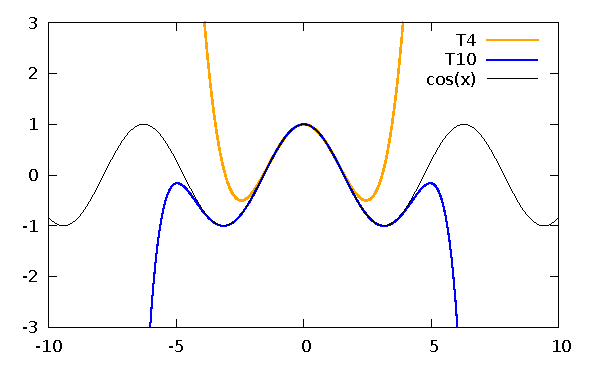
\includegraphics{figures/preliminaries-taylor1}
\par\end{centering}
\end{figure}
 Karena $|R_{n}(x)|$ mengukur secara tepat galat absolut $|T_{n}(x)-f(x)|$,
kita tertarik pada kondisi yang membuat $|R_{n}(x)|$ bernilai kecil.
Menurut pengamatan \ref{enu:taylorObservation2}, ada tiga besaran
yang perlu diperhatikan. Pertama, $|x-x_{0}|^{n+1}$, atau $|x-x_{0}|$,
yaitu jarak antara $x$ dan $x_{0}$. $T_{n}(x)$ pada umumnya memberikan
hampiran yang lebih baik ketika $x$ lebih dekat ke $x_{0}$. Kedua,
$\frac{1}{(n+1)!}$. Hal ini menyiratkan bahwa semakin banyak suku
yang digunakan dalam polinomial Taylor (semakin besar $n$), semakin
baik hampirannya. Terakhir, $|f^{(n+1)}(\xi)|$, yaitu nilai mutlak
turunan berorde $(n+1)$ dari $f$. Semakin terkendali turunan ini,
semakin baik $T_{n}(x)$ menghampiri $f(x)$. Namun, perlu diingat
bahwa semua ini hanyalah pedoman praktis untuk membuat $|R_{n}(x)|$
bernilai kecil. Terdapat pengecualian terhadap pedoman-pedoman tersebut.

Untuk melihat bagaimana ketiga faktor ini bekerja, perhatikan $f(x)=\ln(x)$
yang dikembangkan di sekitar $x_{0}=e^{2}$. Menurut teorema Taylor,
\begin{eqnarray*}
T_{2}(x)=2+\frac{x-e^{2}}{e^{2}}-\frac{(x-e^{2})^{2}}{2e^{4}} & \mbox{ dan } & R_{2}(x)=\frac{1}{3\xi^{3}}(x-e^{2})^{3};\\
T_{11}(x)=2+\sum_{j=1}^{11}\left(\frac{(-1)^{j-1}(x-e^{2})^{j}}{je^{2j}}\right) & \mbox{ dan } & R_{11}(x)=\frac{-1}{12\xi^{12}}(x-e^{2})^{12}.
\end{eqnarray*}
Setelah meyakinkan diri bahwa rumus-rumus ini benar, misalkan kita
ingin menghampiri $\ln(x)$ dengan galat absolut tidak lebih dari
$0.1$. Karena $|\xi^{-3}|$ dan $|\xi^{-12}|$ merupakan fungsi menurun
terhadap $\xi$, keduanya mencapai nilai maksimum pada interval tertutup
di titik ujung kiri interval tersebut. Oleh karena itu, untuk $x\geq e^{2}$,
kita memperoleh $|R_{2}(x)|\leq\max_{\xi\in[e^{2},x]}\left|\frac{1}{3\xi^{3}}(x-e^{2})^{3}\right|=\frac{1}{3e^{6}}(x-e^{2})^{3}$.
Namun, untuk $0<x<e^{2}$, kita memperoleh $|R_{2}(x)|\leq\max_{\xi\in[x,e^{2}]}\left|\frac{1}{3\xi^{3}}(x-e^{2})^{3}\right|=\frac{1}{3x^{3}}(e^{2}-x)^{3}$.
Untuk menentukan nilai peubah yang membuat suku-suku sisa ini lebih
kecil dari $0.1$, kita perlu menyelesaikan persamaan $\frac{1}{3e^{6}}(x-e^{2})^{3}=0.1$
dan $\frac{1}{3x^{3}}(e^{2}-x)^{3}=0.1$. Nilai yang kita cari adalah
$x=\left(1+\sqrt[3]{\frac{3}{10}}\right)e^{2}\approx12.33$ dan $x=\frac{\sqrt[3]{8100}+10\sqrt[3]{90}-30}{13\sqrt[3]{90}}e^{2}\approx4.427$.
Jadi, teorema Taylor menjamin bahwa $T_{2}(x)$ akan menghampiri $\ln(x)$
dengan galat paling besar $0.1$ di seluruh interval $[4.427,12.33]$.
Karena $e^{2}\approx7.389$, $T_{2}(x)$ menghampiri $\ln(x)$ dengan
galat paling besar $0.1$ dari sekitar 3 satuan di bawah $e^{2}$
hingga sekitar 5 satuan di atas $e^{2}$. Dengan kata lain, selama
$x$ cukup dekat dengan $x_{0}=e^{2}$, hampiran tersebut baik. Perhitungan
serupa untuk $R_{11}(x)$ menunjukkan bahwa $T_{11}(x)$ dijamin menghampiri
$\ln(x)$ dengan galat paling besar $0.1$ pada interval $[3.667,14.89]$.
Dengan kata lain, untuk nilai $n$ yang lebih besar, $x$ tidak perlu
sedekat itu dengan $x_{0}$ untuk mencapai akurasi yang sama.

Namun ingatlah, nilai-nilai ini hanyalah batas teoretis bagi galat.
Galat sebenarnya sering kali jauh lebih kecil daripada batas tersebut.
Sebagai contoh, analisis kita memberikan batas atas $|R_{2}(3)|\leq\frac{1}{3\cdot3^{3}}(e^{2}-3)^{3}\approx1.05$
sedangkan galat sebenarnya, $|T_{2}(3)-\ln(3)|=\left|2+\frac{3-e^{2}}{e^{2}}-\frac{(3-e^{2})^{2}}{2e^{4}}-\ln(3)\right|\approx.131$.
Batas tersebut kira-kira 8 kali galat sebenarnya. Jika kita menelaah
hal ini sedikit lebih jauh, grafik $T_{2}(x)$ dan $T_{11}(x)$ dibandingkan
dengan $\ln(x)$ 
\begin{figure}
\caption{\label{fig:taylor3}Galat sebenarnya $|T_{n}(x)-f(x)|$ sering kali
jauh lebih kecil daripada batas teoretis.}

\begin{centering}
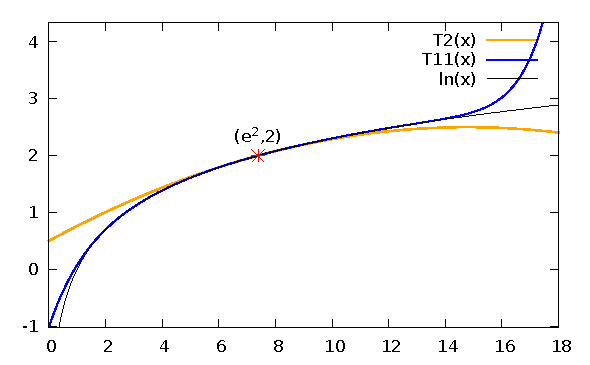
\includegraphics{figures/preliminaries-taylor3}
\par\end{centering}
\end{figure}
 (serta sedikit perhitungan yang akan kita bahas nanti) \label{equationToSolve}
menunjukkan bahwa $T_{2}(x)$ sebenarnya menghampiri $\ln(x)$ dengan
galat paling besar $0.1$ pada interval $[3.296,13.13]$ dan $T_{11}(x)$
sebenarnya menghampiri $\ln(x)$ dengan galat paling besar $0.1$
pada interval $[0.9030,15.33]$. Interval-interval ini sedikit lebih
lebar daripada interval yang dijamin secara teoretis. Lihat Gambar
\ref{fig:taylor3}. Gambar ini juga menunjukkan hal lain. $T_{2}(18)$
jauh lebih baik dalam menghampiri $\ln(18)$ daripada $T_{11}(18)$.
Tidak selalu benar bahwa lebih banyak suku menghasilkan hampiran yang
lebih baik.

Selanjutnya kita membahas polinomial Taylor yang barangkali paling
sering dianalisis---yakni polinomial untuk fungsi sinus dan kosinus.
Keduanya menyajikan contoh dengan visualisasi yang indah dan analisis
yang sederhana.Polinomial Taylor berorde $n$ untuk $f(x)=\cos(x)$
yang dikembangkan di sekitar 0 adalah
\begin{eqnarray*}
T_{n}(x) & = & \cos(0)+\sum_{j=1}^{n}\left(\frac{\left.\frac{d^{j}}{dx^{j}}(\cos(x))\right|_{x=0}}{j!}(x-0)^{j}\right)\\
 & = & \cos(0)-\sin(0)\cdot x-\frac{\cos(0)}{2}x^{2}+\frac{\sin(0)}{6}x^{3}+\frac{\cos(0)}{24}x^{4}-\cdots\\
 & = & 1-\frac{1}{2}x^{2}+\frac{1}{24}x^{4}-\cdots
\end{eqnarray*}
dan suku sisanya adalah 
\begin{eqnarray*}
R_{n}(x) & = & \frac{\left.\frac{d^{n+1}}{dx^{n+1}}(\cos(x))\right|_{x=\xi}}{(n+1)!}(x-0)^{n+1}\\
 & = & \frac{x^{n+1}}{(n+1)!}\begin{cases}
-\sin(\xi) & \mbox{ ketika }n\mbox{ mod }4\equiv0\\
-\cos(\xi) & \mbox{ ketika }n\mbox{ mod }4\equiv1\\
\sin(\xi) & \mbox{ ketika }n\mbox{ mod }4\equiv2\\
\cos(\xi) & \mbox{ ketika }n\mbox{ mod }4\equiv3
\end{cases}.
\end{eqnarray*}
Karena fungsi sinus dan kosinus dibatasi antara $-1$ dan $1$, kita
mengetahui bahwa $-\frac{|x|^{n+1}}{(n+1)!}\leq\frac{x^{n+1}}{(n+1)!}\sin\xi\leq\frac{|x|^{n+1}}{(n+1)!}$
dan demikian pula untuk $-\sin\xi$, $\cos\xi$, serta $-\cos\xi$.
Oleh karena itu, apa pun bentuk suku sisanya,
\[
-\frac{|x|^{n+1}}{(n+1)!}\leq R_{n}(x)\leq\frac{|x|^{n+1}}{(n+1)!}.
\]
Ada dua keadaan yang membuat suku sisa ini bernilai kecil. Pertama,
jika $x$ dekat dengan $0$, maka $|x|$ bernilai kecil sehingga $R_{n}(x)$
bernilai kecil. Kedua, jika $n$ bernilai besar, maka $\frac{1}{(n+1)!}$
bernilai kecil sehingga $R_{n}(x)$ bernilai kecil. Dengan kata lain,
untuk nilai $n$ yang kecil, suku sisanya bernilai kecil ketika nilai
$x$ kecil. $T_{n}(x)$ merupakan hampiran yang baik bagi $\cos(x)$
untuk kombinasi $x$ dan $n$. Sebaliknya, untuk nilai $n$ yang besar,
suku sisanya bernilai kecil bahkan ketika nilai $x$ besar. Sebagai
contoh, $|R_{61}(x)|\leq\frac{|x|^{62}}{62!}$, sehingga $|R_{61}(x)|$
tetap kurang dari 1 untuk semua $x$ yang nilai mutlaknya kurang dari
$\sqrt[62]{62!}\approx23.933$. Gambar \ref{fig:taylor1} dan \ref{fig:taylor2}
mengilustrasikan hal ini. 
\begin{figure}[h]
\caption{\label{fig:taylor2}Untuk $n$ yang besar, $T_{n}(x)$ merupakan hampiran
yang baik bahkan untuk $x$ yang besar.}

\begin{centering}
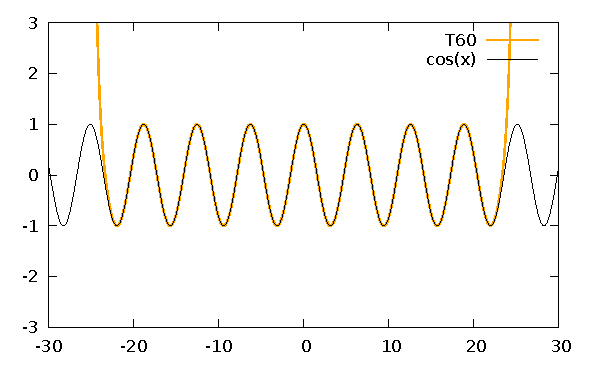
\includegraphics{figures/preliminaries-taylor2}
\par\end{centering}
\end{figure}


\subsection{Konsep Utama}
\begin{description}
\item [{Teorema~Rolle:}] \index{Teorema!Rolle}Misalkan $f(x)$ kontinu
pada $[a,b]$ dan terdiferensialkan pada $(a,b)$. Jika $f(a)=f(b)$,
maka terdapat $\xi\in(a,b)$ sedemikian sehingga $f'(\xi)=0$.
\item [{Teorema~Taylor:}] \index{Teorema!Taylor} Misalkan $f(x)$ memiliki
$n+1$ turunan pada $(a,b)$, dan $x_{0}\in(a,b)$. Maka, untuk setiap
$x\in(a,b)$, terdapat $\xi$, yang bergantung pada $x$, dan terletak
di antara $x$ dan $x_{0}$ tanpa sama dengan keduanya, sedemikian
sehingga
\[
f(x)=f(x_{0})+\sum_{j=1}^{n}\left(\frac{f^{(j)}(x_{0})}{j!}(x-x_{0})^{j}\right)+\frac{f^{(n+1)}(\xi)}{(n+1)!}(x-x_{0})^{n+1}.
\]
\item [{$n$~polinomial~Taylor:}] \index{polinomial!Taylor}\index{Taylor!polinomial}
$T_{n}(x)=f(x_{0})+\sum_{j=1}^{n}\left(\frac{f^{(j)}(x_{0})}{j!}(x-x_{0})^{j}\right)$.
\item [{Polinomial~Maclaurin:}] \index{polinomial!Maclaurin}Polinomial
Taylor yang dikembangkan di sekitar $x_{0}=0$ juga disebut \index{polinomial Maclaurin}polinomial
Maclaurin.
\item [{Suku~sisa:}] $R_{n}(x)=\frac{f^{(n+1)}(\xi)}{(n+1)!}(x-x_{0})^{n+1}$
tepat sama dengan $-\left(T_{n}(x)-f(x)\right)$.
\item [{Suku~galat:}] Nama lain untuk suku sisa.
\end{description}
\begin{digression}{Teorema asli Brook Taylor} 

\noindent Teorema asli \index{Teorema!Taylor} karya Brook Taylor
\index{Taylor!Brook} diterbitkan dalam karya besarnya \textit{Methodus
Incrementorum Directa \& Inversa} pada tahun 1715. Di dalam \textit{Methodus},
teorema ini muncul sebagai korolari kedua dari Proposisi VII Teorema
III dan nyaris tidak menyerupai pernyataan modern mana pun dari teorema
tersebut. 

\begin{center}
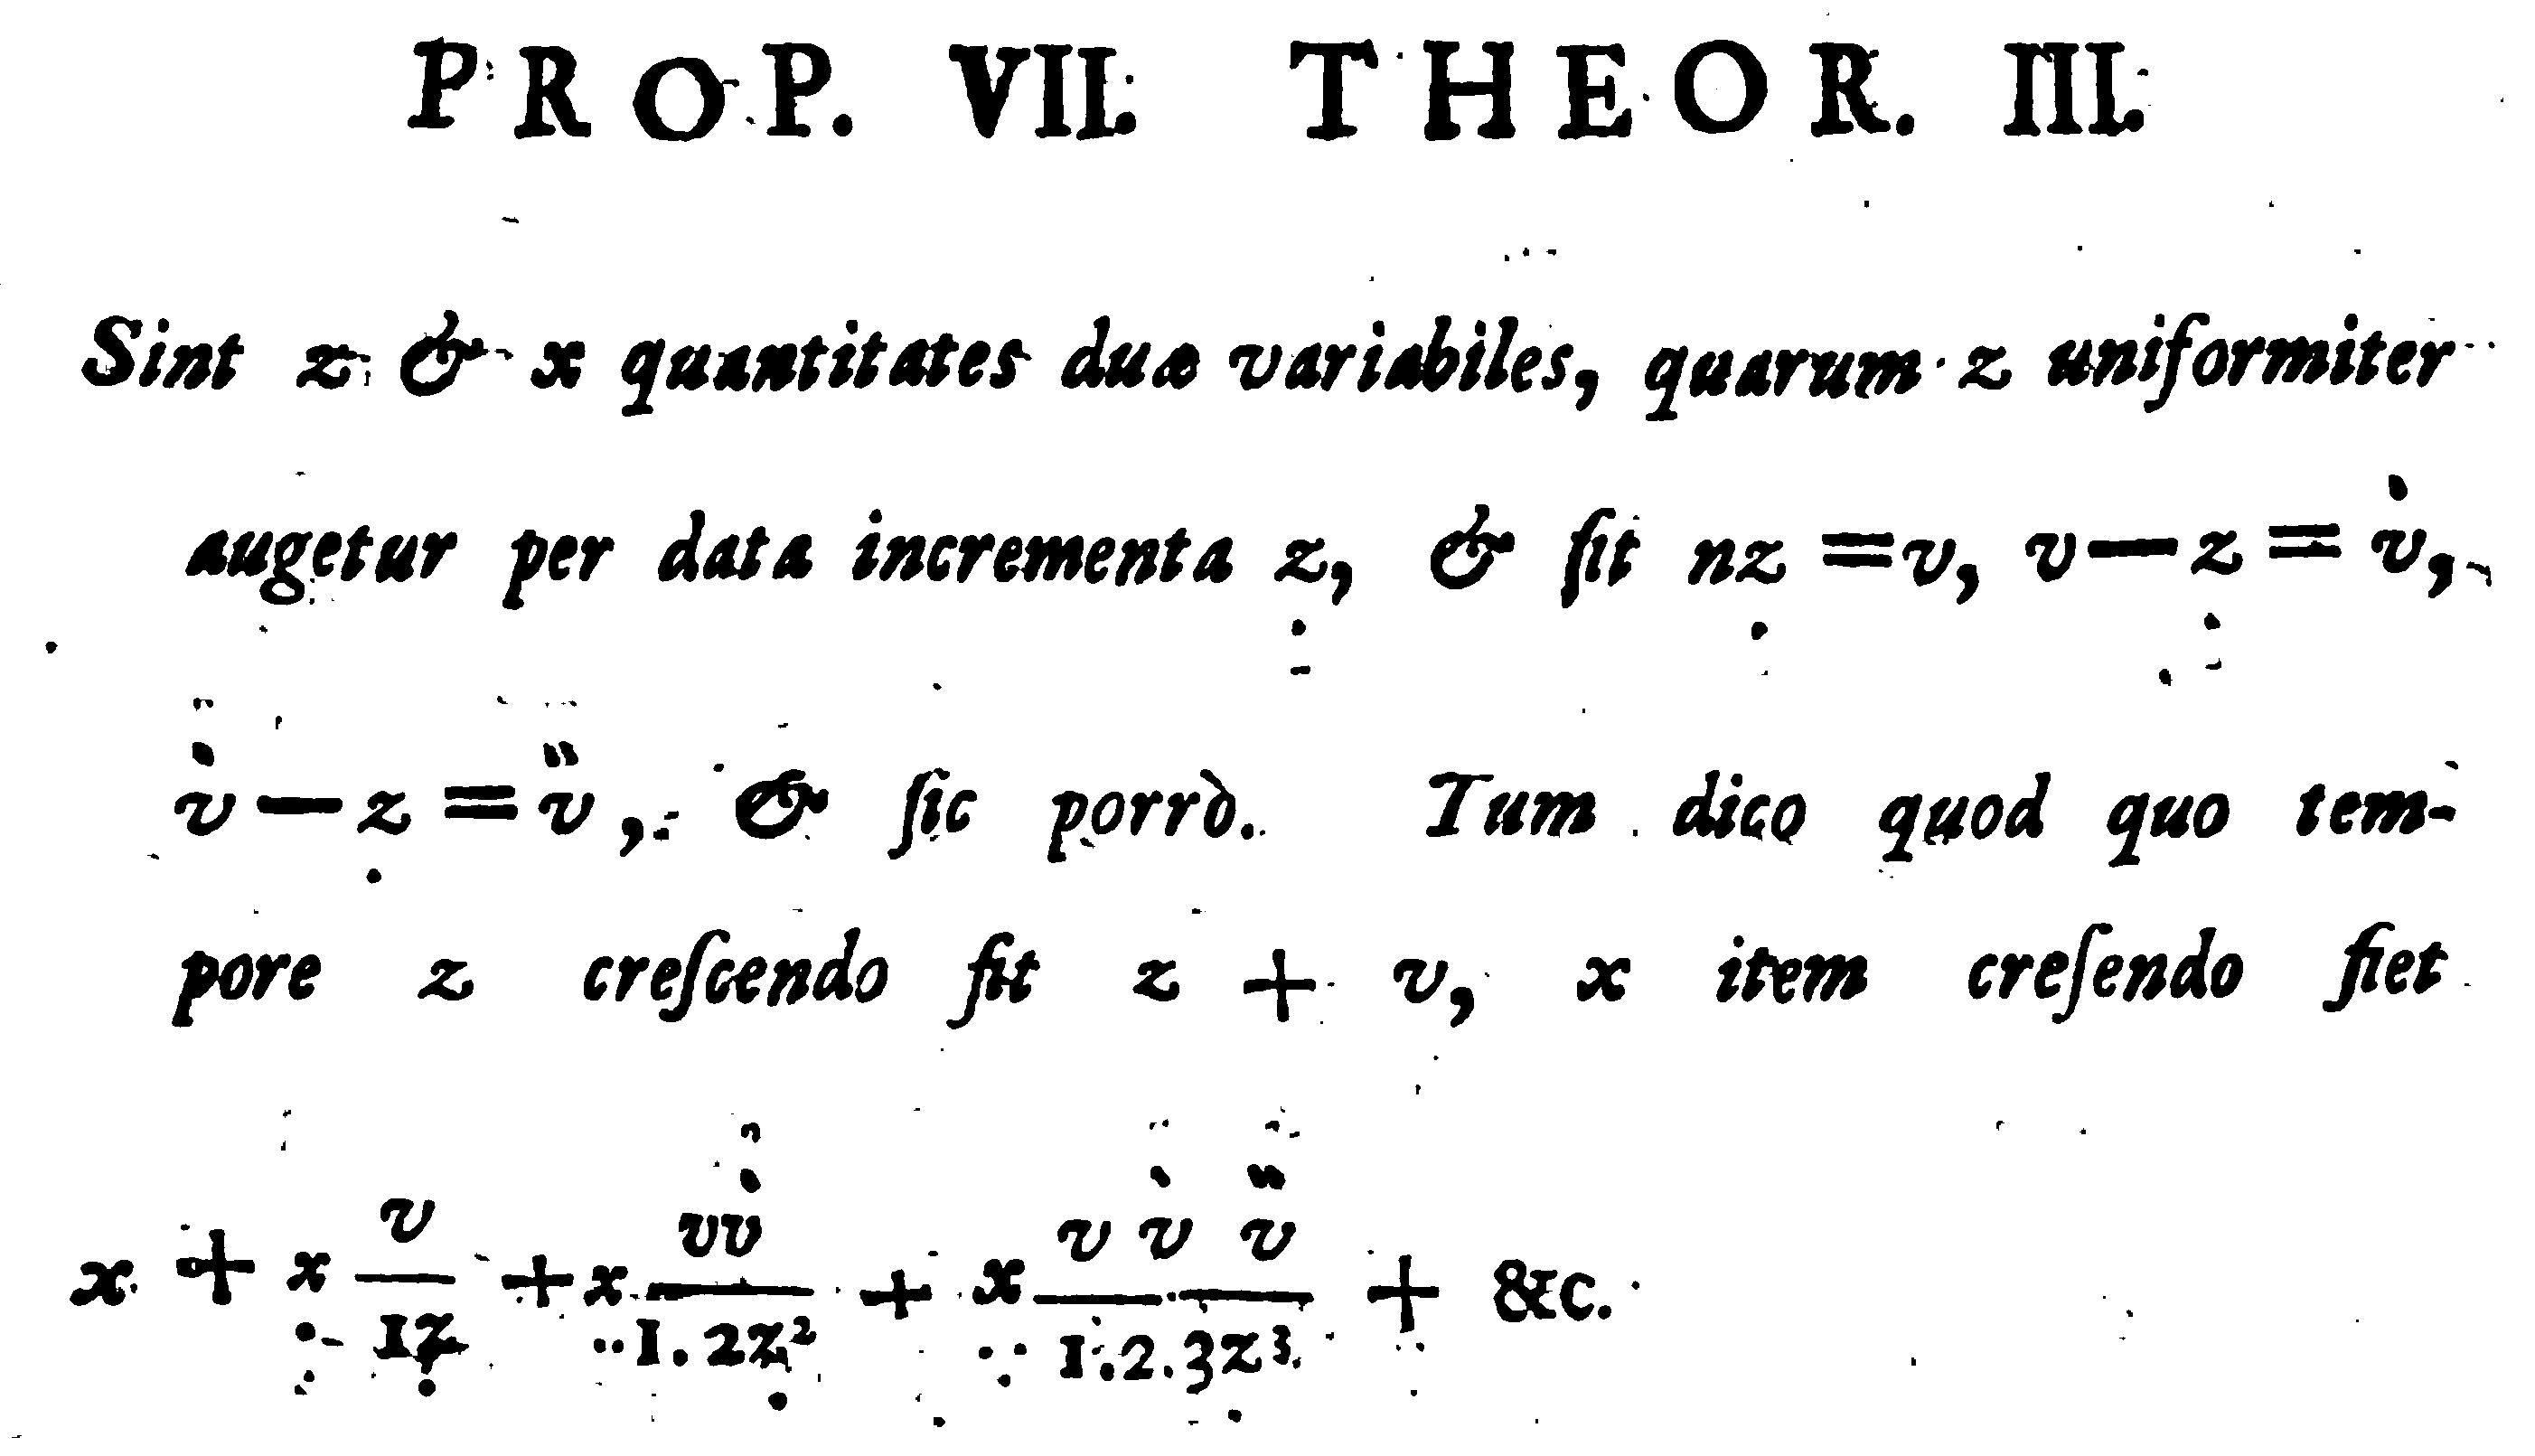
\includegraphics[scale=0.11]{figures/Taylor--MethodusPage21}
\par\end{center}

\begin{center}
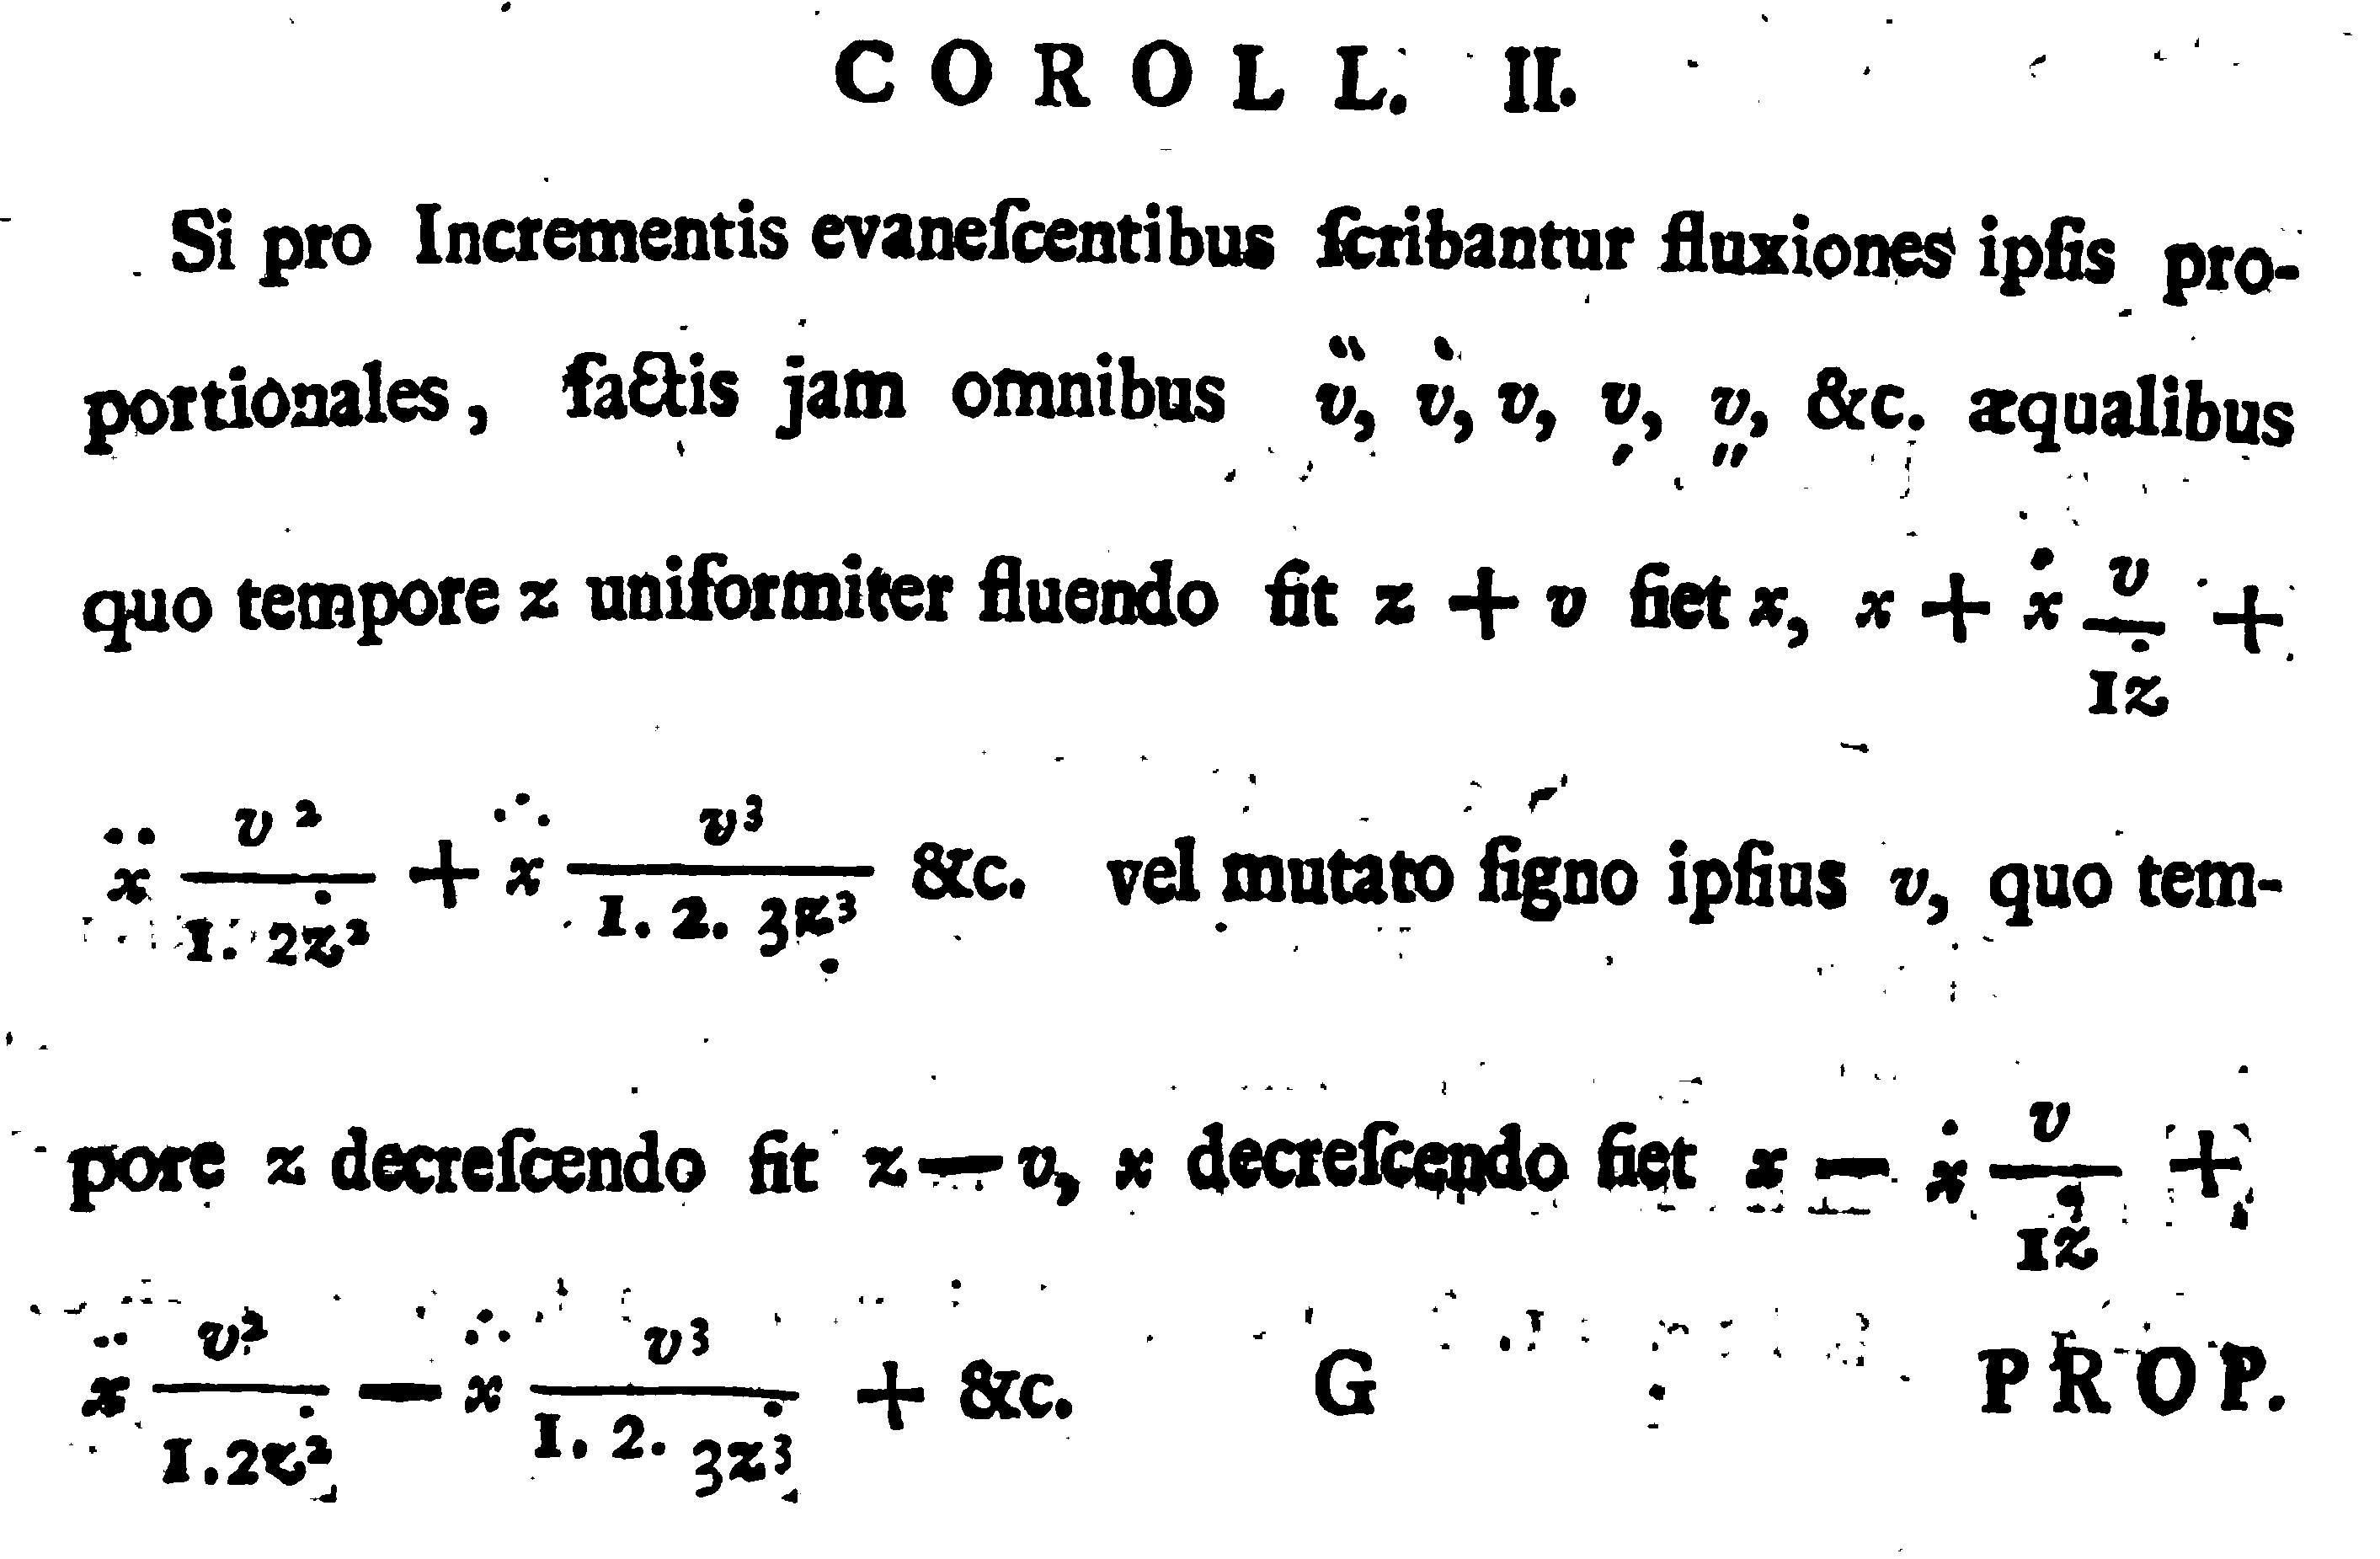
\includegraphics[scale=0.11]{figures/Taylor--MethodusPage23}
\par\end{center}

\noindent Tidak ada penyebutan suku sisa. Notasi fungsi $f(x)$ yang
lazim tidak digunakan. Teksnya ditulis dalam bahasa Latin. Dan tidak
ada daftar panjang hipotesis.

Berikut pernyataan asli teorema Taylor dalam bahasa Inggris sebagaimana
diterjemahkan oleh Ian Bruce.\textsc{ Proposisi VII. Teorema III:}
Terdapat dua besaran variabel, $z$ \& $x$, dengan $z$ bertambah
secara teratur sebesar pertambahan yang diberikan $\underset{\dot{\ }}{z}$,
dan $n\underset{\dot{\ }}{z}=v$, $v-\underset{\dot{\ }}{z}=\overset{^{\backslash}}{v}$,
$\overset{^{\backslash}}{v}-\underset{\dot{\ }}{z}=\overset{^{\backslash\backslash}}{v}$,
dan seterusnya. Selanjutnya, saya menyatakan bahwa selama waktu $z$
bertambah menjadi $z+v$, $x$ juga bertambah menjadi $x+\underset{\dot{\ }}{x}\frac{v}{1\underset{\dot{\ }}{z}}+\underset{\ddot{\ }}{x}\frac{v\overset{\backslash}{v}}{1\cdot2\underset{\dot{\ }}{z}^{2}}+\underset{\dddot{\ }}{x}\frac{v\overset{\backslash}{v}\overset{\backslash\backslash}{v}}{1\cdot2\cdot3\underset{\dot{\ }}{z}^{3}}+\mbox{\&c}$.\textsc{
Korolari II:} Jika untuk pertambahan yang melenyap, fluksion dari
besaran-besaran yang sebanding itu sendiri dituliskan, kini dengan
semua $\overset{^{\backslash\backslash}}{v},\ \overset{^{\backslash}}{v},\ v,\ \underset{^{/}}{v},\ \underset{^{//}}{v},\mbox{ \&c.}$
sama dengan waktu $z$ yang mengalir seragam hingga menjadi $z+v$,
$x$ menjadi $x+\dot{x}\frac{v}{1\dot{z}}+\ddot{x}\frac{v^{2}}{1\cdot2\dot{z}^{2}}+\dddot{x}\frac{v^{3}}{1\cdot2\cdot3\dot{z}^{3}}+\mbox{\&c }\ldots$

\end{digression}

\begin{digression}{Penafsiran teorema asli Brook Taylor} 

\noindent Sayangnya, terjemahan bahasa Inggris teorema Taylor hanya
cukup membantu bagi orang yang tidak akrab dengan matematika awal
abad ke-$18$. Pada tahun 1715, notasi fungsi masih baru akan muncul
20 tahun kemudian. Saat ini, kita akan menafsirkan deklarasi kedua
variabel itu sebagai pernyataan bahwa $x$ merupakan fungsi dari $z$.
Klaim dalam Teorema III adalah bahwa kita dapat menulis ulang $x(z+v)$
sebagai $x+\underset{\dot{\ }}{x}\frac{v}{1\underset{\dot{\ }}{z}}+\underset{\ddot{\ }}{x}\frac{v\overset{\backslash}{v}}{1\cdot2\underset{\dot{\ }}{z}^{2}}+\underset{\dddot{\ }}{x}\frac{v\overset{\backslash}{v}\overset{\backslash\backslash}{v}}{1\cdot2\cdot3\underset{\dot{\ }}{z}^{3}}+\mbox{\&c}$.
Sama seperti $x$ harus ditafsirkan sebagai fungsi dari $z$, demikian
pula $\underset{\dot{\ }}{x}$, $\underset{\ddot{\ }}{x}$, dan $\underset{\dddot{\ }}{x}$.
Lebih tepatnya, $\underset{\dot{\ }}{x}$ berarti $x(z+\underset{\dot{\ }}{z})-x(z)$,
yaitu besarnya pertambahan $x$ ketika $z$ ditambah sebesar $\underset{\dot{\ }}{z}$.
Demikian pula, $\underset{\ddot{\ }}{x}$ adalah besarnya pertambahan
$\underset{\dot{\ }}{x}$ ketika $z$ ditambah sebesar $\underset{\dot{\ }}{z}$,
sehingga $\underset{\ddot{\ }}{x}=\underset{\dot{\ }}{x}(z+\underset{\dot{\ }}{z})-\underset{\dot{\ }}{x}(z)=\left[x(z+2\underset{\dot{\ }}{z})-x(z+\underset{\dot{\ }}{z})\right]-\left[x(z+\underset{\dot{\ }}{z})-x(z)\right]=x(z+2\underset{\dot{\ }}{z})-2x(z+\underset{\dot{\ }}{z})+x(z)$.
Serupa dengan itu, $\underset{\dddot{\ }}{x}$ adalah besarnya pertambahan
$\underset{\ddot{\ }}{x}$ ketika $z$ ditambah sebesar $\underset{\dot{\ }}{z}$.
Sekarang saat yang tepat untuk berhenti membaca sejenak dan memverifikasi
bahwa $\underset{\dddot{\ }}{x}=x(z+3\underset{\dot{\ }}{z})-3x(z+2\underset{\dot{\ }}{z})+3x(z+\underset{\dot{\ }}{z})-x(z)$,
bahwa $\underset{\ddddot{\ }}{x}=x(z+4\underset{\dot{\ }}{z})-4x(z+3\underset{\dot{\ }}{z})+6x(z+2\underset{\dot{\ }}{z})-4x(z+\underset{\dot{\ }}{z})+x(z)$,
dan seterusnya. Dengan pemahaman ini serta konvensi $\underset{0}{x}$
untuk $x$, $\underset{1}{x}$ untuk $\underset{\dot{\ }}{x}$, $\underset{2}{x}$
untuk $\underset{\ddot{\ }}{x}$, $\overset{0}{v}$ untuk $v$, $\overset{1}{v}$
untuk $\overset{^{\backslash}}{v}$, $\overset{2}{v}$ untuk $\overset{^{\backslash\backslash}}{v}$,
dan seterusnya, dapat ditunjukkan melalui latihan aljabar bahwa
\begin{eqnarray*}
x(z+n\underset{\dot{\ }}{z}) & = & \sum_{j=0}^{n}\left(\begin{array}{c}
n\\
j
\end{array}\right)\underset{^{j}}{x}=\underset{^{0}}{x}+\underset{^{1}}{x}\frac{n}{1}+\underset{^{2}}{x}\frac{n(n-1)}{1\cdot2}+\underset{^{3}}{x}\frac{n(n-1)(n-2)}{1\cdot2\cdot3}+\cdots+\underset{^{n}}{x}\frac{n(n-1)\cdots1}{1\cdot2\cdot3\cdots n}\\
 & = & \underset{^{0}}{x}+\underset{^{1}}{x}\frac{n\underset{\dot{\ }}{z}}{1\underset{\dot{\ }}{z}}+\underset{^{2}}{x}\frac{n\underset{\dot{\ }}{z}(n-1)\underset{\dot{\ }}{z}}{1\cdot2\underset{\dot{\ }}{z}^{2}}+\underset{^{3}}{x}\frac{n\underset{\dot{\ }}{z}(n-1)\underset{\dot{\ }}{z}(n-2)\underset{\dot{\ }}{z}}{1\cdot2\cdot3\underset{\dot{\ }}{z}^{3}}+\cdots+\underset{^{n}}{x}\frac{n\underset{\dot{\ }}{z}(n-1)\underset{\dot{\ }}{z}\cdots1\underset{\dot{\ }}{z}}{1\cdot2\cdot3\cdots n\underset{\dot{\ }}{z}^{n}}\\
 & = & \underset{^{0}}{x}+\underset{^{1}}{x}\frac{v}{1\underset{\dot{\ }}{z}}+\underset{^{2}}{x}\frac{v\overset{1}{v}}{1\cdot2\underset{\dot{\ }}{z}^{2}}+\underset{^{3}}{x}\frac{v\overset{2}{v}\overset{3}{v}}{1\cdot2\cdot3\underset{\dot{\ }}{z}^{3}}+\cdots+\underset{^{n}}{x}\frac{v\overset{2}{v}\overset{3}{v}\cdots\overset{n}{v}}{1\cdot2\cdot3\cdots n\underset{\dot{\ }}{z}^{n}}.
\end{eqnarray*}
Perhitungan ini pada dasarnya merupakan pembuktian Taylor untuk Teorema
III. 

Korolari II (yang akan kita anggap sebagai teorema) tidak dibuktikan
oleh Taylor selain melalui penerapan yang ``jelas'' dari teori fluksion
Newton. Dalam bahasa sekarang, Korolari II diperoleh dengan mengambil
limit ketika $n\to\infty$ pada ekspresi dari Teorema III. Latihan
menarik lainnya adalah memverifikasi bahwa $\lim_{n\to\infty}\frac{\underset{k}{x}}{\underset{\dot{\ }}{z}^{k}}=x^{(k)}(z)$,
yaitu turunan berorde $k$ dari $x$. Dan satu latihan terakhir untuk
melihat bahwa $\lim_{n\to\infty}\overset{k}{v}=v$. Sebagaimana Taylor
menganggap hasil-hasil ini begitu saja, demikian pula kita. Dengan
menerapkannya pada Teorema III, kita memperoleh $x(z+v)=x(z)+x'(z)\frac{v}{1!}+x''(z)\frac{v^{2}}{2!}+x'''(z)\frac{v^{3}}{3!}+\cdots$.
Dalam notasi Taylor, $\frac{\dot{x}}{\dot{z}}$ adalah turunan pertama
dari $x$, $\frac{\ddot{x}}{\dot{z}^{2}}$ adalah turunan kedua dari
$x$, dan seterusnya. Jadi, kita memang memperoleh $x+\dot{x}\frac{v}{1\dot{z}}+\ddot{x}\frac{v^{2}}{1\cdot2\dot{z}^{2}}+\dddot{x}\frac{v^{3}}{1\cdot2\cdot3\dot{z}^{3}}+\mbox{\&c}$
sebagaimana diklaim.

Menarik bahwa Teorema III berlaku untuk fungsi $x$ apa pun yang didefinisikan
pada interval $[x,x+v]$. Tidak menjadi masalah apakah $x$ terdiferensialkan,
atau bahkan kontinu. Teorema ini merupakan pernyataan tentang beda
hingga. Justru korolarinya memerlukan jauh lebih banyak asumsi karena
di sanalah kita beralih ke limit. \end{digression} 

\subsection{Octave}

Dua hal yang akan berulang kali berguna ketika menggunakan Octave
adalah fungsi anonim \index{Octave!fungsi anonim} dan berkas \texttt{.m}\index{Octave!berkas .m@berkas \texttt{.m}}.
Membuat fungsi anonim merupakan cara sederhana untuk membuat fungsi
``khusus'' dalam Octave. Membuat berkas \texttt{.m} merupakan cara
yang teratur untuk menjalankan sejumlah perintah dan menyimpan pekerjaan
Anda untuk digunakan kemudian. 

Pada bagian sebelumnya kita melihat banyak fungsi bawaan seperti \texttt{sin(x)},
\texttt{log(x)}, dan \texttt{abs(x)}. Fungsi-fungsi ini memiliki makna
yang telah ditentukan dalam Octave. Namun, bagaimana jika Anda ingin
mendefinisikan $f(x)=3x^{2}$? Tidak ada fungsi bawaan ``3 $x$ kuadrat''.
Di sinilah fungsi anonim berguna. Sintaks fungsi anonim adalah

\begin{center}
\texttt{nama = @(variabel) definisi fungsi}
\par\end{center}

\noindent di mana \texttt{nama} adalah nama fungsi,\texttt{ variabel}
adalah daftar variabel yang digunakan dalam fungsi dan dipisahkan
dengan koma, sedangkan \texttt{definisi fungsi} adalah rumusnya. Untuk
$f(x)=3x^{2}$, kode Octave-nya adalah \texttt{f=@(x) 3{*}x\textasciicircum 2}.
Selanjutnya Anda dapat menggunakan \texttt{f} dengan cara yang sama
seperti menggunakan \texttt{sin}, \texttt{log} atau \texttt{abs}.
Ketik nama fungsi, tanda kurung buka, argumen, lalu tanda kurung tutup.
Jadi, setelah mendefinisikan \texttt{f} dengan pernyataan \texttt{f=@(x)
3{*}x\textasciicircum 2}, \texttt{f(7)} akan menghasilkan 147: \begin{verbatim}
octave:1> f=@(x) 3*x^2;
octave:2> f(7)
ans =  147 
\end{verbatim}

Sekarang kita dapat menyelesaikan Percobaan 1 pada bagian \ref{sec:Accuracy}
dengan cara keempat. Alih-alih melakukan perhitungan pada baris perintah,
kita dapat membuat berkas teks yang memuat perintah-perintah tersebut.
Setelah disimpan sebagai berkas \texttt{.m}, Octave akan mengenalinya
sebagai daftar instruksi. Jika Anda terbiasa dengan pemrograman, cara
bekerja dengan Octave ini akan terasa sangat alami. Menulis berkas
\texttt{.m} setara dengan menulis sebuah program. Setelah ditulis,
berkas tersebut perlu diproses. Pada baris perintah Octave, berkas
\texttt{.m} dijalankan dengan mengetikkan nama berkas tanpa akhiran
\texttt{.m}. Hanya itu, sehingga prosesnya tidak persis seperti menulis
sebuah program. Tidak ada proses kompilasi. Dalam hal ini, prosesnya
lebih menyerupai pembuatan skrip. 

Untuk memulai, gunakan editor teks apa pun yang Anda sukai untuk membuat
daftar perintah. Perhatikan baik-baik: Microsoft Word, LibreOffice,
dan pengolah kata lainnya bukanlah editor teks. Program-program tersebut
adalah pengolah kata. Pengolah kata memiliki fitur pemformatan huruf,
pengaturan halaman, dan sebagainya. Sekarang bayangkan laporan terakhir
atau surat Anda kepada Ibu, lalu hapus semua pemformatannya kecuali
pemisah antarparagraf. Itulah berkas teks. Tidak ada cetak tebal,
pemusatan, gambar, huruf khusus, margin, ataupun halaman. Hanya kata-kata
yang diketik. Segala hiasan yang disediakan pengolah kata tidak diperlukan.
Octave hanya memerlukan daftar perintah. Pemformatan yang diperlukan
hanyalah ganti baris dan tab. Jika Anda belum memiliki editor teks
favorit---dan mungkin sekalipun sudah---gunakanlah editor yang disertakan
bersama Octave. Dengan program tersebut, Anda tidak akan mengalami
masalah. Jika Anda menggunakan Octave Online atau CoCalc, platform
daring itu menyediakan editor; gunakanlah editor tersebut. 

Dengan editor teks pilihan Anda, buatlah dokumen teks \texttt{experiment1.m}
persis seperti yang ditampilkan berikut ini: \begin{verbatim}
format('long')
p1 = 10*pi-31
p2 = 100*p1-41
p3 = 100*p2-59
p4 = 100*p3-26
p5 = 100*p4-53
p6 = 100*p5-58
p7 = 100*p6-97 
\end{verbatim} Kemudian, pada baris perintah Octave, ketik \texttt{experiment1}
untuk memperoleh hasilnya: \begin{verbatim}
octave:1> experiment1
p1 =  0.415926535897931
p2 =  0.592653589793116
p3 =  0.265358979311600
p4 =  0.535897931159980
p5 =  0.589793115997963
p6 =  0.979311599796347
p7 =  0.931159979634685
\end{verbatim} Cara menulis perintah Octave ini memiliki dua keunggulan yang jelas.
Pertama, jika Anda membuat kesalahan, memperbaikinya sangat mudah.
Cukup sunting berkas teks tersebut dan simpan perubahannya. Kedua,
Anda memiliki catatan pekerjaan Anda. Anda dapat membagikan, mencetak,
atau sekadar menyimpannya untuk digunakan kemudian. Hanya ada satu
kekurangan nyata. Cara ini lebih rumit daripada sekadar menjalankan
beberapa perintah pada baris perintah. Karena itu, untuk perhitungan
sederhana, cara ini lebih merepotkan daripada yang diperlukan.

Perhatikan bahwa berkas \texttt{.m} harus disimpan dalam direktori
yang sama dengan tempat Octave dijalankan. Jika Anda menggunakan lingkungan
pengembangan terintegrasi (IDE), perincian semacam ini akan ditangani
untuk Anda. Namun, jika Anda menggunakan baris perintah dan editor
teks, pastikan berkas \texttt{.m} disimpan di lokasi yang benar.

\noindent\startexercises

\subsection{Latihan}
\begin{enumerate}
\item Tentukan $T_{3}(x)$ dan $R_{3}(x)$ untuk fungsi yang dikembangkan
di sekitar $x_{0}$.

\begin{enumerate}
\item \label{exc:taylor1}$f(x)=\sin(x)$; $x_{0}=0$. \hasasolution 
\item $f(x)=\sin(x)$; $x_{0}=\pi/2$.
\item \label{exc:taylor2}$f(x)=\sin(x)$; $x_{0}=\pi$. \hasasolution 
\item $f(x)=e^{x}$; $x_{0}=0$.
\item $f(x)=e^{x}$; $x_{0}=\ln2$.
\item \label{exc:taylor3}$f(x)=x\sin(x)$; $x_{0}=0$. \hasananswer 
\item $f(x)=\cos^{2}(x)$; $x_{0}=0$.
\end{enumerate}
\item Misalkan $f(x)=4x^{3}-2x^{2}+8x-9$.

\begin{enumerate}
\item Tentukan $T_{3}(x)$ dan $R_{3}(x)$ untuk pengembangan di sekitar
$x_{0}=0$.
\item Tentukan $T_{3}(x)$ dan $R_{3}(x)$ untuk pengembangan di sekitar
$x_{0}=2$.
\item Rumuskan suatu konjektur berdasarkan jawaban Anda untuk bagian (a)
dan (b). Dapatkah Anda membuktikannya?
\end{enumerate}
\item Tentukan polinomial Maclaurin berindeks $36$ untuk $f(x)=e^{x}$.
\item Misalkan $f(x)$ adalah fungsi yang memiliki turunan keempat pada
seluruh garis bilangan real, $(-\infty,\infty)$, dan memenuhi $f(2)=3$,
$f'(2)=-1$, $f''(2)=2$, serta $f'''(2)=-1$.

\begin{enumerate}
\item Tuliskan polinomial Taylor derajat ketiga untuk $f(x)$ yang dikembangkan
di sekitar $x_{0}=2$.
\item Gunakan polinomial Taylor tersebut untuk menghampiri $f(4)$.
\item Tentukan suatu batas atas bagi galat absolut hampiran tersebut dengan
memanfaatkan fakta bahwa
\[
-3\leq f^{(4)}(\xi)\leq5
\]
untuk setiap $\xi\in[2,4]$.
\end{enumerate}
\item Hitung polinomial Taylor berindeks $3$ untuk $f(x)=x^{5}-2x^{4}+x^{3}-9x^{2}+x-1$
yang dikembangkan di sekitar $x_{0}=1$.
\item Tentukan polinomial Taylor derajat kedua untuk $f(x)=\csc x$ yang
dikembangkan di sekitar ${\displaystyle x_{0}=\frac{\pi}{4}}$. Berikut
beberapa fakta yang mungkin berguna:
\begin{gather*}
f'(x)=-\csc(x)\cot(x)\quad\csc(x)=\frac{1}{\sin(x)}\\
f''(x)=\csc(x)(1+2\cot^{2}(x))\quad\cot(x)=\frac{\cos(x)}{\sin(x)}
\end{gather*}
\item Sinus hiperbolik, $\sinh(x)$, dan kosinus hiperbolik, $\cosh(x)$,
saling merupakan turunan. Artinya, 
\[
\begin{gathered}\frac{\textrm{d}}{\textrm{d}x}(\sinh(x))=\cosh(x)\\
\textrm{dan}\\
\frac{\textrm{d}}{\textrm{d}x}(\cosh(x))=\sinh(x).
\end{gathered}
\]
Tentukan suku sisa, $R_{43}$, yang terkait dengan polinomial Maclaurin
berindeks $43$ untuk $f(x)=\cosh(x)$. 
\item \octave\ \label{exc:taylor8}Gunakan fungsi anonim untuk menghitung
nilai polinomial Taylor $T_{4}(x)=1-\frac{1}{2}x^{2}+\frac{1}{24}x^{4}$
pada nilai $x$ yang diberikan. \hasasolution 

\begin{enumerate}
\item 0
\item $\frac{1}{2}$
\item 1
\item $\pi$
\end{enumerate}
\item \octave\ \label{exc:taylor10}Gunakan fungsi anonim untuk menghitung
nilai polinomial Taylor $T_{3}(x)=1+x+\frac{1}{2}x^{2}+\frac{1}{6}x^{3}$
pada nilai $x$ yang diberikan.

\begin{enumerate}
\item 0
\item $\frac{3}{2}$
\item $2$
\item \label{exc:taylor9}$e$ \hasananswer 
\end{enumerate}
\item \octave\ \label{exc:taylor11}Tulis dan jalankan sebuah berkas \texttt{.m}
yang menghitung semua jawaban untuk latihan \ref{exc:taylor8}. \hasasolution 
\item \octave\ Tulis dan jalankan sebuah berkas \texttt{.m} yang menghitung
semua jawaban untuk latihan \ref{exc:taylor10}.
\item Tentukan $\xi(x)$ yang keberadaannya dijamin oleh teorema Taylor
dalam setiap situasi berikut.

\begin{enumerate}
\item \label{exc:taylor7}$f(x)=\cos(x)$, $x_{0}=0$, $n=3$, $x=\pi$. \hasananswer 
\item $f(x)=e^{x}$, $x_{0}=0$, $n=3$, $x=\ln4$.
\item $f(x)=\ln(x)$, $x_{0}=1$, $n=4$, $x=2$.
\end{enumerate}
\item Misalkan $f(x)=x^{3}$.

\begin{enumerate}
\item Tentukan polinomial Taylor derajat kedua, $P_{2}(x)$, yang dikembangkan
di sekitar $x_{0}=0$.
\item Tentukan suku sisa, $R_{2}(0.5)$, serta galat sebenarnya yang timbul
ketika $P_{2}(0.5)$ digunakan untuk menghampiri $f(0.5)$.
\item Ulangi bagian (a) dengan menggunakan $x_{0}=1$.
\item Ulangi bagian (b) dengan menggunakan polinomial dari bagian (c).
\end{enumerate}
\item Tentukan polinomial Taylor derajat kedua, $P_{2}(x)$, untuk $f(x)=e^{x}\cos x$
yang dikembangkan di sekitar $x_{0}=0$.

\begin{enumerate}
\item Gunakan $P_{2}(0.5)$ untuk menghampiri $f(0.5)$. Tentukan batas
atas bagi galat $|f(0.5)-P_{2}(0.5)|$ dengan menggunakan suku sisa,
lalu bandingkan batas tersebut dengan galat sebenarnya.
\item Tentukan suatu batas bagi galat $|f(x)-P_{2}(x)|$ yang berlaku untuk
seluruh interval $[0,1]$.
\item Hampiri $\int_{0}^{1}f(x)\,dx$ dengan menghitung $\int_{0}^{1}P_{2}(x)\,dx$
sebagai gantinya.
\item Tentukan batas atas bagi galat pada bagian (c) dengan menggunakan
$\int_{0}^{1}|R_{2}(x)|\,dx$ dan bandingkan batas tersebut dengan
galat sebenarnya.
\end{enumerate}
\item Misalkan $f(x)=e^{x}$.

\begin{enumerate}
\item Tentukan polinomial Maclaurin berindeks $n$ $P_{n}(x)$ untuk $f(x)$.
\item Tentukan batas galat ketika $P_{4}(2)$ digunakan untuk menghampiri
$f(2)$.
\item Berapa banyak suku polinomial Maclaurin yang perlu digunakan untuk
menghampiri $f(2)$ dengan galat tidak lebih dari $10^{-10}$? Dengan
kata lain, untuk nilai $n$ berapakah $P_{n}(2)$ memiliki batas galat
yang kurang dari atau sama dengan $10^{-10}$?
\end{enumerate}
\item Tentukan polinomial Taylor derajat keempat untuk $\ln x$ yang dikembangkan
di sekitar $x_{0}=1$. 
\item Apa suku berindeks $50$ dari $T_{100}(e^{x})$ yang dikembangkan
di sekitar $x_{0}=6$?
\item \label{arctan}Deret Maclaurin untuk fungsi arkustangen konvergen
pada $-1<x\leq1$ dan diberikan oleh
\[
\arctan x=\lim_{n\to\infty}P_{n}(x)=\lim_{n\to\infty}\sum_{i=1}^{n}(-1)^{i-1}\frac{x^{2i-1}}{2i-1}.
\]
Gunakan fakta bahwa $\tan(\pi/4)=1$ untuk menentukan banyaknya suku,
$n$, dalam deret yang harus dijumlahkan untuk memastikan bahwa $|4P_{n}(1)-\pi|<10^{-3}$.
\item Latihan \ref{arctan} menguraikan cara yang kurang efisien untuk memperoleh
hampiran bagi $\pi$. Metode tersebut dapat diperbaiki secara berarti
dengan mengamati bahwa $\pi/4=\arctan\frac{1}{2}+\arctan\frac{1}{3}$
serta menghitung deret arkustangen pada $\frac{1}{2}$ dan pada $\frac{1}{3}$.
Tentukan banyaknya suku yang harus dijumlahkan agar diperoleh hampiran
bagi $\pi$ dengan galat tidak lebih dari $10^{-3}$.
\item Untuk $f(x)=\tan^{-1}(x)$, 
\[
f^{(n)}(0)=\begin{cases}
0 & \textrm{jika }n\textrm{ genap}\\
(-1)^{(n-1)/2}(n-1)! & \textrm{jika }n\textrm{ ganjil}.
\end{cases}
\]
tentukan polinomial Maclaurin berindeks $n$ $P_{n}(x)$ untuk $f$.
\item Berapa banyak suku deret Maclaurin untuk $\sin x$ yang diperlukan
untuk menjamin hampiran dengan galat tidak lebih dari $10^{-2}$ bagi
setiap nilai $x$ antara 0 dan $2\pi$?
\item Misalkan Anda menghampiri $f(x)=e^{x}$ menggunakan polinomial Maclaurin
derajat kesepuluh. Tentukan interval terbesar yang menjamin hampiran
tersebut memiliki galat tidak lebih dari $10^{-3}$.
\item Tentukan batas galat dalam menghampiri $e^{10}$ dengan menggunakan
polinomial Taylor derajat kedua puluh lima dari $g(x)=e^{x}$ yang
dikembangkan di sekitar $x_{0}=0$.
\item Tentukan batas galat hampiran 
\[
e^{2}\approx1+2+\frac{1}{2}(2)^{2}+\frac{1}{6}(2)^{3}+\frac{1}{24}(2)^{4}+\frac{1}{120}(2)^{5}
\]
menurut teorema Taylor. Bandingkan batas ini dengan galat sebenarnya.
\item Misalkan $f^{(8)}(x)=e^{x}\cos x$ untuk suatu fungsi $f$. Tentukan
batas galat dalam menghampiri $f(x)$ pada interval $[0,\pi/2]$ dengan
menggunakan $T_{7}(x)$ yang dikembangkan di sekitar $x_{0}=0$.
\item \label{exc:taylor4}Misalkan $f(x)=\frac{1}{x}$, dan $x_{0}=5$. \hasasolution 

\begin{enumerate}
\item Tentukan $T_{2}(x)$.
\item Tentukan $R_{2}(x)$.
\item Gunakan $T_{2}(x)$ untuk menghampiri $f(1)$ dan $f(9)$.
\item Tentukan batas atas teoretis bagi galat absolut setiap hampiran pada
bagian (c).
\item Tentukan batas bawah teoretis bagi galat absolut setiap hampiran pada
bagian (c).
\item Tentukan galat absolut sebenarnya untuk setiap hampiran pada bagian
(c). Verifikasi bahwa galat-galat tersebut memang berada di antara
batas-batas teoretis.
\item Buat sketsa grafik $f(x)$ dan $T_{2}(x)$ pada sistem sumbu yang
sama untuk $x\in[1,9]$.
\end{enumerate}
\item Misalkan $f(x)=\ln(1+x)$ dan $x_{0}=0$.

\begin{enumerate}
\item Tentukan $T_{3}(x)$.
\item Tentukan $R_{3}(x)$.
\item Gunakan $T_{3}(x)$ untuk menghampiri $f(1)$ dan $f(26)$.
\item Tentukan batas atas teoretis bagi galat absolut setiap hampiran pada
bagian (c).
\item Tentukan batas bawah teoretis bagi galat absolut setiap hampiran pada
bagian (c).
\item Tentukan galat absolut sebenarnya untuk setiap hampiran pada bagian
(c). Verifikasi bahwa galat-galat tersebut memang berada di antara
batas-batas teoretis.
\item Buat sketsa grafik $f(x)$ dan $T_{3}(x)$ pada sistem sumbu yang
sama untuk $x\in[1,26]$.
\end{enumerate}
\item Misalkan $f(x)$ memenuhi $-3\leq f^{(10)}(x)\leq7$ untuk setiap
$x\in[0,10]$. Tentukan batas bawah dan batas atas bagi galat absolut
ketika $T_{9}(x)$ yang dikembangkan di sekitar $x_{0}=3$ digunakan
untuk menghampiri

\begin{enumerate}
\item $f(0)$.
\item $f(10)$.
\end{enumerate}
\item Misalkan Anda ingin menghampiri nilai $-e^{4}\sin4$ dengan menggunakan
polinomial Maclaurin terpisah (polinomial Taylor yang dikembangkan
di sekitar $x_{0}=0$) untuk fungsi sinus dan eksponensial, alih-alih
menggunakan satu polinomial Maclaurin untuk fungsi $f(x)=-e^{x}\sin x$.
Berapa banyak suku dari masing-masing polinomial yang diperlukan untuk
memperoleh galat tidak lebih dari $10^{-20}$? Abaikan galat pembulatan.
\item Tentukan batas atas teoretis, sebagai fungsi dari $x$, bagi galat
absolut ketika $T_{4}(x)$ digunakan untuk menghampiri $f(x)$.

\begin{enumerate}
\item $e^{x}\sin x$; $x_{0}=0$.
\item \label{exc:taylor5}$e^{-x^{2}}$; $x_{0}=0$. \hasasolution 
\item $\frac{10}{x}+\sin(10x)$; $x_{0}=\pi$.
\end{enumerate}
\item Deret Maclaurin untuk $f(x)=e^{-x}$ adalah
\[
\sum_{i=0}^{\infty}\frac{(-1)^{i}}{i!}x^{i}=1-x+\frac{1}{2}x^{2}-\frac{1}{6}x^{3}+\ldots
\]
 Tentukan batas galat dalam menghampiri $1/e$ dengan $1-1+1/2-1/6+1/24$.
\item Deret Taylor untuk $f(x)=e^{x}$ adalah ${\displaystyle T(x)=1+x+\frac{1}{2!}x^{2}+\frac{1}{3!}x^{3}+\frac{1}{4!}x^{4}+\frac{1}{5!}x^{5}+\cdots}$.
Deret ini konvergen ke $f(x)$ untuk semua nilai $x$. Khususnya,
untuk $x=1$, hal ini berarti bahwa
\[
f(1)=T(1)=1+1+\frac{1}{2!}(1)^{2}+\frac{1}{3!}(1)^{3}+\frac{1}{4!}(1)^{4}+\cdots
\]
Dengan menyederhanakan persamaan ini, kita memperoleh
\[
e=1+1+\frac{1}{2}+\frac{1}{6}+\frac{1}{24}+\frac{1}{120}+\cdots
\]
Gunakan deret Taylor untuk menentukan deret tak hingga yang jumlahnya
sama dengan 

\begin{enumerate}
\item $\ln(2)$
\item $2/3$
\item $\pi/4$
\item $\sqrt{2}$
\end{enumerate}
\end{enumerate}
\finishexercises



\section{\label{sec:Speed}Kecepatan}

Selain akurasi, tidak ada hal yang lebih penting dalam metode numerik
daripada kecepatan. Namun, hampir selalu terdapat kompromi di antara
keduanya. Perhitungan cepat sering kali tidak terlalu akurat, sedangkan
perhitungan akurat sering kali tidak terlalu cepat. Meskipun demikian,
algoritme tertentu menghasilkan nilai akurat dengan cepat. Menurunkan
algoritme semacam itu, atau mengenalinya setelah diturunkan, merupakan
inti analisis numerik.

Jenis metode numerik pertama yang akan kita temui menghasilkan barisan
hampiran yang, jika semuanya bekerja dengan baik, mendekati suatu
nilai yang diinginkan, misalnya $p$. Dengan metode ini, kita akan
memperoleh barisan $\langle p_{n}\rangle$ dengan $\lim_{n\to\infty}p_{n}=p$.
Anda seharusnya sudah mengenal konsep limit barisan dari Kalkulus,
tetapi tujuannya di sana sangat berbeda dari tujuan kita di sini.
Umumnya, perhatian Anda tertuju pada apakah suatu barisan konvergen
atau tidak. Jika barisan tersebut konvergen dan Anda sangat beruntung,
Anda dapat menentukan limitnya. Dalam analisis numerik, kita mengetahui
bahwa barisan tertentu konvergen dan hanya tertarik pada seberapa
cepat kekonvergenan itu terjadi. 

Pengamatan sederhana (dan sedikit akal sehat) dapat menunjukkan mobil
mana di jalan raya yang melaju lebih cepat daripada mobil lainnya.
Pengamatan sederhana (dan sedikit akal sehat) juga sering dapat menunjukkan
barisan mana yang konvergen lebih cepat daripada barisan lainnya.
\begin{table}[h]
\hrule \caption{\label{tab:convergenceTo2.718281828...}Beberapa barisan yang konvergen
ke $e$.}
\medskip{}

\centering{}%
\begin{tabular}{c|cccc}
$n$ & $q_{n}$ & $r_{n}$ & $s_{n}$ & $t_{n}$\tabularnewline
\hline 
0 & 3 & 3 & 3 & 3\tabularnewline
1 & $2.9436563656918$ & $2.86799618929986$ & $2.82129001274358$ & $2.78177393100014$\tabularnewline
2 & $2.89858145824525$ & $2.78315514435127$ & $2.73850656616954$ & $2.72150682612711$\tabularnewline
3 & $2.86252153228801$ & $2.73974041668143$ & $2.71973377603211$ & $2.71829014894701$\tabularnewline
4 & $2.83367359152222$ & $2.72324781752852$ & $2.71830229432561$ & $2.71828182851442$\tabularnewline
5 & $2.81059523890958$ & $2.71899828870116$ & $2.71828184916891$ & $2.71828182845904$\tabularnewline
6 & $2.79213255681947$ & $2.71833715075158$ & $2.71828182845934$ & $2.71828182845904$\tabularnewline
7 & $2.77736241114739$ & $2.71828369688657$ & $2.71828182845904$ & $2.71828182845904$\tabularnewline
8 & $2.76554629460972$ & $2.71828184959225$ & $2.71828182845904$ & $2.71828182845904$\tabularnewline
9 & $2.75609340137958$ & $2.71828182851528$ & $2.71828182845904$ & $2.71828182845904$\tabularnewline
10 & $2.74853108679547$ & $2.71828182845907$ & $2.71828182845904$ & $2.71828182845904$\tabularnewline
$\vdots$ & $\vdots$ & $\vdots$ & $\vdots$ & $\vdots$\tabularnewline
\end{tabular}\medskip{}
\hrule 
\end{table}
 Perhatikan barisan-barisan dalam Tabel \ref{tab:convergenceTo2.718281828...}
yang semuanya konvergen ke $e\approx2.71828182845904$. $\langle t_{n}\rangle$
sudah akurat hingga 15 angka signifikan pada suku keenam; $\langle s_{n}\rangle$
sudah akurat hingga 15 angka signifikan pada suku kedelapan; $\langle r_{n}\rangle$
masih belum akurat hingga 15 angka signifikan pada suku kesebelas,
tetapi tampaknya akan mencapai akurasi 15 angka signifikan pada suku
kedua belas; sedangkan $\langle q_{n}\rangle$ baru akurat hingga
2 angka signifikan pada suku kesebelas, sehingga tampaknya memerlukan
jauh lebih dari dua belas suku untuk mencapai akurasi 15 angka signifikan.
Karena semuanya dimulai dari 3, cukup masuk akal untuk mengatakan
bahwa, jika diurutkan dari yang tercepat hingga yang paling lambat,
urutannya adalah $\langle t_{n}\rangle$, $\langle s_{n}\rangle$,
$\langle r_{n}\rangle$, $\langle q_{n}\rangle$. Dan urutan itu memang
benar, sebagaimana akan segera kita lihat. Namun, mengetahui mobil
mana yang lebih cepat berbeda dengan mengetahui kecepatan masing-masing
mobil. Demikian pula, mengetahui barisan mana yang konvergen lebih
cepat berbeda dengan mengetahui seberapa cepat masing-masing barisan
itu konvergen. Untuk mengukur kecepatan mobil tertentu, Anda memerlukan
speedometer atau alat pengukur kecepatan radar. Untuk mengukur orde
kekonvergenan (kecepatan) suatu barisan, Anda memerlukan sebuah definisi
dan sedikit aljabar. 

\subsubsection{Orde kekonvergenan suatu barisan\index{kekonvergenan!orde}}

Misalkan barisan $\langle p_{n}\rangle$ konvergen ke $p$. Kita mengatakan
bahwa $\langle p_{n}\rangle$ konvergen dengan orde $\alpha\geq1$
jika
\[
\lim_{n\to\infty}\frac{\left|p_{n+1}-p\right|}{\left|p_{n}-p\right|^{\alpha}}=\lambda
\]
untuk suatu bilangan real $\lambda>0$. 

Mari kita lihat cara menggunakan definisi ini untuk menghitung orde
kekonvergenan barisan-barisan dalam Tabel \ref{tab:convergenceTo2.718281828...}.
Menurut definisi tersebut, $\alpha$, jika ada, menyatakan kecepatan
(atau orde) kekonvergenan \index{kekonvergenan!orde} suatu barisan.
Sekarang, dengan mengasumsikan bahwa $\alpha$ memang ada, kita memperoleh
$\lim_{n\to\infty}\frac{\left|p_{n+1}-p\right|}{\left|p_{n}-p\right|^{\alpha}}=\lambda$,
sehingga untuk $n$ yang cukup besar,
\[
\frac{\left|p_{n+1}-p\right|}{\left|p_{n}-p\right|^{\alpha}}\approx\frac{\left|p_{n+2}-p\right|}{\left|p_{n+1}-p\right|^{\alpha}}\approx\lambda.
\]
Secara khusus, kita dapat menyelesaikan persamaan tersebut terhadap
$\alpha$ dan memperoleh ${\displaystyle \alpha\approx\frac{\ln\left|\frac{p_{n+2}-p}{p_{n+1}-p}\right|}{\ln\left|\frac{p_{n+1}-p}{p_{n}-p}\right|}}$.

\begin{digression}{Orde kekonvergenan kurang dari atau sama dengan 1?} 

\noindent Tidak ada orde kekonvergenan \index{kekonvergenan!orde}
yang kurang dari satu, sebab jika $\lim_{n\to\infty}\frac{\left|p_{n+1}-p\right|}{\left|p_{n}-p\right|^{\alpha}}=\lambda$
untuk suatu $0<\alpha<1$, maka 
\begin{eqnarray*}
\lim_{n\to\infty}\frac{|p_{n+1}-p|}{|p_{n}-p|} & = & \lim_{n\to\infty}\frac{|p_{n+1}-p|}{|p_{n}-p|^{\alpha}}\cdot|p_{n}-p|^{\alpha-1},
\end{eqnarray*}
yang merupakan kontradiksi. Di satu sisi, uji rasio menyiratkan bahwa
$\lim_{n\to\infty}\frac{|p_{n+1}-p|}{|p_{n}-p|}$ ada dan kurang dari
atau sama dengan 1. Di sisi lain, $\alpha<1\implies\alpha-1<0$ sehingga
ketika $|p_{n}-p|$ bernilai kecil, $|p_{n}-p|^{\alpha-1}$ bernilai
besar. Oleh karena itu, $\lim_{n\to\infty}\frac{|p_{n+1}-p|}{|p_{n}-p|^{\alpha}}\cdot|p_{n}-p|^{\alpha-1}$
tidak ada. Untuk membuktikannya secara ketat, misalkan $M$ adalah
sebarang bilangan real. Maka terdapat $N_{1}$ sedemikian sehingga
$n>N_{1}$ menyiratkan $\frac{|p_{n+1}-p|}{|p_{n}-p|^{\alpha}}>0.9\lambda$.
Terdapat pula $N_{2}$ sedemikian sehingga $n>N_{2}$ menyiratkan
${\displaystyle |p_{n}-p|<\left(\frac{0.9\lambda}{M}\right)^{\frac{1}{1-\alpha}}}$,
sehingga $|p_{n}-p|^{\alpha-1}>\frac{M}{0.9\lambda}$. Dengan mengambil
$N=\max\{N_{1},N_{2}\}$, kita memperoleh bahwa $n>N$ menyiratkan
sekaligus $\frac{|p_{n+1}-p|}{|p_{n}-p|^{\alpha}}>0.9\lambda$ dan
$|p_{n}-p|^{\alpha-1}>\frac{M}{0.9\lambda}$. Oleh karena itu, untuk
$n>N$, berlaku 
\begin{eqnarray*}
\frac{|p_{n+1}-p|}{|p_{n}-p|} & = & \frac{|p_{n+1}-p|}{|p_{n}-p|^{\alpha}}\cdot|p_{n}-p|^{\alpha-1}>0.9\lambda\cdot\frac{M}{0.9\lambda}=M.
\end{eqnarray*}
Dengan demikian, $\lim_{n\to\infty}\frac{|p_{n+1}-p|}{|p_{n}-p|}$
tidak ada. Ketika $\alpha=1$, haruslah $\lambda\leq1$ karena jika
tidak, uji rasio menyiratkan bahwa $\langle|p_{n}-p|\rangle$ divergen
dan, dengan demikian, $\langle p_{n}\rangle$ divergen. 

\noindent\end{digression} 

Sebagai contoh, ${\displaystyle \frac{\ln\left|\frac{q_{2}-e}{q_{1}-e}\right|}{\ln\left|\frac{q_{1}-e}{q_{0}-e}\right|}\approx\frac{\ln\left|\frac{2.8985-e}{2.9436-e}\right|}{\ln\left|\frac{2.9436-e}{3-e}\right|}}\approx1$
dan ${\displaystyle \frac{\ln\left|\frac{q_{10}-e}{q_{9}-e}\right|}{\ln\left|\frac{q_{9}-e}{q_{8}-e}\right|}=\frac{\ln\left|\frac{2.7485-e}{2.7560-e}\right|}{\ln\left|\frac{2.7560-e}{2.7655-e}\right|}}\approx1$.
Jika kita mencoba kelompok lain yang terdiri atas tiga suku berurutan
dari $\langle q_{n}\rangle$, kita memperoleh hasil yang sama. Orde
kekonvergenan\index{kekonvergenan!orde} dari $\langle q_{n}\rangle$
kira-kira 1. Tentu saja, kita memerlukan rumus untuk $|q_{n}-e|$
guna menentukan apakah limit tersebut benar-benar 1, tetapi kita sudah
memiliki beberapa bukti pendukung. Dengan mengulangi perhitungan untuk
$\langle r_{n}\rangle$, $\langle s_{n}\rangle$, dan $\langle t_{n}\rangle$,
kita memperoleh perkiraan orde kekonvergenan masing-masing sebesar
$1.322$, $1.618$, dan $2$. Sekali lagi kita melihat bahwa, jika
diurutkan dari yang tercepat hingga yang paling lambat, urutannya
adalah $\langle t_{n}\rangle$, $\langle s_{n}\rangle$, $\langle r_{n}\rangle$,
$\langle q_{n}\rangle$. 

Jika Anda mencoba menghitung sendiri orde kekonvergenan tersebut,
mungkin Anda menyadari bahwa diperlukan informasi tambahan untuk menggunakan
$s_{n}$ ketika $n>6$ atau $t_{n}$ ketika $n>4$. Semua suku tersebut
bernilai sama di dalam tabel, sehingga rumus untuk $\alpha$ gagal
menghasilkan bilangan real! Tabel yang lebih berguna untuk menghitung
orde kekonvergenan adalah tabel yang memuat galat absolut: 
\begin{table}[h]
\hrule \caption{\label{tab:absoluteErrors}Galat absolut.}
\medskip{}

\centering{}%
\begin{tabular}{c|cccc}
$n$ & $|q_{n}-e|$ & $|r_{n}-e|$ & $|s_{n}-e|$ & $|t_{n}-e|$\tabularnewline
\hline 
0 & $2.817(10)^{-1}$ & $2.817(10)^{-1}$ & $2.817(10)^{-1}$ & $2.817(10)^{-1}$\tabularnewline
1 & $2.253(10)^{-1}$ & $1.497(10)^{-1}$ & $1.03(10)^{-1}$ & $6.349(10)^{-2}$\tabularnewline
2 & $1.802(10)^{-1}$ & $6.487(10)^{-2}$ & $2.022(10)^{-2}$ & $3.224(10)^{-3}$\tabularnewline
3 & $1.442(10)^{-1}$ & $2.145(10)^{-2}$ & $1.451(10)^{-3}$ & $8.32(10)^{-6}$\tabularnewline
4 & $1.153(10)^{-1}$ & $4.965(10)^{-3}$ & $2.046(10)^{-5}$ & $5.538(10)^{-11}$\tabularnewline
5 & $9.231(10)^{-2}$ & $7.164(10)^{-4}$ & $2.07(10)^{-8}$ & $2.453(10)^{-21}$\tabularnewline
6 & $7.385(10)^{-2}$ & $5.532(10)^{-5}$ & $2.953(10)^{-13}$ & $4.817(10)^{-42}$\tabularnewline
7 & $5.908(10)^{-2}$ & $1.868(10)^{-6}$ & $4.263(10)^{-21}$ & $1.856(10)^{-83}$\tabularnewline
8 & $4.726(10)^{-2}$ & $2.113(10)^{-8}$ & $8.777(10)^{-34}$ & $2.757(10)^{-166}$\tabularnewline
9 & $3.781(10)^{-2}$ & $5.623(10)^{-11}$ & $2.608(10)^{-54}$ & $6.084(10)^{-332}$\tabularnewline
10 & $3.024(10)^{-2}$ & $2.22(10)^{-14}$ & $1.595(10)^{-87}$ & $2.961(10)^{-663}$\tabularnewline
\end{tabular}\medskip{}
\hrule 
\end{table}
 Selain mempermudah penghitungan $\alpha$, tabel ini menunjukkan
dengan sangat jelas bahwa simpulan berdasarkan intuisi kita tentang
barisan mana yang berkonvergensi lebih cepat memang benar. Bandingkan
saja akurasi (galat absolut) suku kesebelasnya. 

Sekarang kita dapat menghitung orde kekonvergenan\index{kekonvergenan!orde},
tetapi apa sebenarnya maknanya? Apa yang diberitahukan orde kekonvergenan
tentang suku-suku berurutan dalam barisan? Dengan menyelesaikan hampiran
$\frac{\left|p_{n+1}-p\right|}{\left|p_{n}-p\right|^{\alpha}}\approx\lambda$
kita peroleh $|p_{n+1}-p|\approx\lambda|p_{n}-p|^{\alpha}$. Jadi,
secara kasar, kekonvergenan berorde $\alpha$ berarti bahwa, untuk
$n$ yang cukup besar, hampiran $p_{n+1}$ sekitar $\lambda|p_{n}-p|^{\alpha-1}$
kali lebih dekat ke limit $p$ daripada $p_{n}$. Untuk menyatakannya
kembali dalam banyaknya angka signifikan yang akurat, kita lakukan
sedikit aljabar:
\begin{eqnarray*}
|p_{n+1}-p| & \approx & \lambda|p_{n}-p|^{\alpha}\\
\left|\frac{p_{n+1}-p}{p}\right| & \approx & \lambda\left|\frac{p_{n}-p}{p}\right|^{\alpha}\cdot|p|^{\alpha-1}\\
-\log\left|\frac{p_{n+1}-p}{p}\right| & \approx & -\log\left|\frac{p_{n}-p}{p}\right|^{\alpha}-\log\left(\lambda|p|^{\alpha-1}\right)\\
d(p_{n+1}) & \approx & \alpha d(p_{n})-\log\left(\lambda|p|^{\alpha-1}\right).
\end{eqnarray*}
Berdasarkan perhitungan ini, kita memperoleh aturan praktis berikut:
\begin{enumerate}
\item untuk kekonvergenan linear ($\alpha=1$), $d(p_{n+1})\approx d(p_{n})-\log\lambda$,
sehingga setiap suku memiliki sejumlah tetap angka signifikan yang
akurat lebih banyak (kira-kira sama dengan $-\log\lambda$) dibanding
suku sebelumnya;
\item untuk kekonvergenan kuadratik ($\alpha=2$), $d(p_{n+1})\approx2d(p_{n})-\log\left(\lambda|p|\right)$,
sehingga setiap suku memiliki kira-kira dua kali banyaknya angka signifikan
yang akurat dibanding suku sebelumnya, dengan sedikit penyimpangan;
\item untuk kekonvergenan kubik ($\alpha=3$), $d(p_{n+1})\approx3d(p_{n})-\log\left(\lambda|p|^{2}\right)$,
sehingga setiap suku memiliki kira-kira tiga kali banyaknya angka
signifikan yang akurat dibanding suku sebelumnya, dengan sedikit penyimpangan;
\end{enumerate}
dan seterusnya. Ringkasnya, untuk $n$ yang besar, setiap suku diperkirakan
memiliki $-\log\left(\lambda|p|^{\alpha-1}\right)$ angka signifikan
akurat lebih banyak daripada $\alpha$ kali banyaknya angka signifikan
akurat pada suku sebelumnya. Kita dapat melihat klaim ini secara langsung
dengan menghitung $\lambda$ untuk barisan $\langle t_{n}\rangle$,
$\langle s_{n}\rangle$, $\langle r_{n}\rangle$, dan $\langle q_{n}\rangle$.
Dengan menggunakan fakta bahwa $\lambda\approx\frac{\left|p_{n+1}-p\right|}{\left|p_{n}-p\right|^{\alpha}}$,
kita peroleh $\lambda=0.8$ untuk setiap barisan. Oleh karena itu,
pada $\langle q_{n}\rangle$, setiap suku seharusnya memiliki $-\log0.8\approx.1$
angka signifikan akurat lebih banyak daripada suku sebelumnya. Dalam
istilah yang lebih mudah dipahami, barisan itu memperoleh sekitar
satu angka signifikan akurat tambahan setiap sepuluh suku. Hal ini
tampak dari pengamatan bahwa $q_{0}$ memiliki galat sekitar $3(10)^{-1}$,
sedangkan $q_{10}$ memiliki galat sekitar $3(10)^{-2}$. Untuk $\langle r_{n}\rangle$,
setiap suku diperkirakan memiliki sekitar $-\log(0.8\cdot e^{.322})\approx-0.04$
angka signifikan akurat lebih banyak daripada $1.322$ kali banyaknya
angka signifikan akurat pada suku sebelumnya. Sebagai contoh, $r_{3}$
memiliki sekitar $\log\left|\frac{e}{2.145(10)^{-2}}\right|\approx2.1$
angka signifikan akurat, sedangkan $r_{4}$ memiliki sekitar $1.322(2.1)-.04\approx2.73$
angka signifikan akurat, $r_{5}$ memiliki $1.322(2.73)-.04\approx3.57$
angka signifikan akurat, dan seterusnya hingga $r_{8}$ memiliki sekitar
$8.1$ angka signifikan akurat. Hal ini kembali ditegaskan oleh tabel,
karena $\log\left|\frac{e}{r_{8}-e}\right|=\log\left|\frac{e}{2.113(10)^{-8}}\right|\approx8.1$.
Walaupun kita dapat melakukan perhitungan serupa untuk $\langle t_{n}\rangle$,
lebih mudah untuk menilainya secara langsung karena yang perlu kita
perhatikan hanyalah bahwa eksponen dalam notasi ilmiah kira-kira menjadi
dua kali lipat dari satu suku ke suku berikutnya. Memang demikian:
eksponennya berubah dari 1 menjadi 2, lalu 3, 6, 11, dan seterusnya. 

Perhatikan bahwa dalam seluruh analisis ini, kita telah mengabaikan
syarat bahwa $n$ harus ``besar''. Hal itu dapat diterima dalam
kasus ini karena barisan-barisan tersebut sengaja dirancang sedemikian
rupa sehingga bahkan $n=0$ pun sudah cukup besar! Dalam penerapan
praktis, tidak demikian.

Untuk memahami betapa jauh lebih cepat suatu orde kekonvergenan dibanding
orde lainnya, tinjau kembali relasi 
\[
d(p_{n+1})\approx\alpha d(p_{n})-\log\left(\lambda|p|^{\alpha-1}\right)
\]
. Sekarang, anggaplah kita mengetahui bahwa $d(p_{n_{0}})=d_{n_{0}}$
untuk suatu $n_{0}$ tertentu yang cukup besar sehingga hampiran tersebut
masuk akal. Maka dapat ditunjukkan bahwa, untuk $\alpha>1$, 
\[
d(p_{n_{0}+k})\approx(d_{n_{0}}-C)\alpha^{k}+C
\]
dengan ${\displaystyle C=\frac{\log\left(\lambda|p|^{\alpha-1}\right)}{\alpha-1}}$. 

\begin{digression}{Menyelesaikan Relasi Rekurensi} 

\noindent Relasi $d(p_{n+1})\approx\alpha d(p_{n})-\log\left(\lambda|p|^{\alpha-1}\right)$
merupakan contoh relasi rekurensi. Secara khusus, relasi tersebut
merupakan relasi rekurensi linear takhomogen orde pertama dengan koefisien
konstan karena berbentuk
\[
a_{n+1}=k_{1}a_{n}+k_{2}
\]
dengan $k_{1}$ dan $k_{2}$ adalah konstanta. Relasi rekurensi linear
takhomogen dapat diselesaikan dengan menjumlahkan solusi homogen dan
solusi partikular. Untuk solusi partikular, kita mencari solusi berbentuk
$a_{n}=A$ (untuk semua $n$) dengan menyubstitusikan solusi yang
diasumsikan ini ke dalam relasi rekurensi. Penyubstitusian itu menghasilkan
$A=k_{1}A+k_{2}$, sehingga $A=\frac{k_{2}}{1-k_{1}}$ merupakan solusi
semacam itu. Untuk solusi homogen, kita mencari barisan berbentuk
$a_{n}=r^{n}$ yang memenuhi $a_{n+1}=k_{1}a_{n}+0$. Dengan menyubstitusikan
solusi yang diasumsikan ke dalam relasi rekurensi yang telah diubah
(homogen), kita peroleh $r^{n+1}=k_{1}r^{n}$. Dengan menata ulang,
$r^{n}(r-k_{1})=0$ sehingga $r=0$ atau $r=k_{1}$. Perhatikan bahwa
$Bk_{1}^{n}$ juga merupakan solusi untuk sembarang konstanta $B$.
Hal ini mencakup solusi $a_{n}=0$ yang diperoleh dengan menetapkan
$r=0$. Akhirnya, dengan menggabungkan solusi partikular dan solusi
homogen, solusi dari $a_{n+1}=k_{1}a_{n}+k_{2}$ adalah $a_{n}=Bk_{1}^{n}+\frac{k_{2}}{1-k_{1}}$
untuk sembarang konstanta $B$. Dalam kasus $d(p_{n+1})\approx\alpha d(p_{n})-\log\left(\lambda|p|^{\alpha-1}\right)$,
$k_{1}=\alpha$ dan $k_{2}=-\log\left(\lambda|p|^{\alpha-1}\right)$
sehingga $d(p_{n})=B\alpha^{n}+\frac{\log\left(\lambda|p|^{\alpha-1}\right)}{\alpha-1}$.
Nilai $B$ ditentukan dengan menyubstitusikan sembarang unsur barisan
yang diketahui ke dalam rumus ini, lalu menyelesaikannya untuk $B$.
Jika $d(p_{n_{0}})=d_{n_{0}}$, diperoleh $d(p_{n})=\left(d_{n_{0}}-\frac{\log\left(\lambda|p|^{\alpha-1}\right)}{\alpha-1}\right)\alpha^{n}+\frac{\log\left(\lambda|p|^{\alpha-1}\right)}{\alpha-1}$. 

\noindent\end{digression}  

\noindent Hal penting yang perlu diperhatikan di sini ialah bahwa
$d(p_{n_{0}+k})$ merupakan fungsi eksponensial ketika $\alpha>1$.
Banyaknya angka signifikan yang akurat bertumbuh secara eksponensial
dengan basis $\alpha$. Seperti yang telah kita lihat, untuk $\alpha=1$,
banyaknya angka signifikan bertumbuh secara linear. Dalam kalkulus,
Anda telah mempelajari bahwa setiap fungsi eksponensial bertumbuh
jauh lebih cepat daripada setiap fungsi polinomial. Oleh karena itu,
wajar dan benar untuk menyimpulkan bahwa barisan yang konvergen dengan
orde lebih besar daripada $1$ berkonvergensi jauh lebih cepat daripada
barisan dengan orde linear ($\alpha=1$). 

Namun, berhati-hatilah. Berdasarkan pengetahuan kalkulus yang sama,
Anda juga akan menyimpulkan bahwa barisan $\langle2^{-n}\rangle$
konvergen ke 0 jauh lebih cepat daripada $\langle n^{-2}\rangle$.
Menurut sebagian ukuran, hal itu benar, tetapi tidak menurut semua
ukuran. Tinjau orde kekonvergenan kedua barisan tersebut. Kita mencari
nilai $\alpha_{1}$ dan $\alpha_{2}$ sedemikian sehingga
\[
\lim_{n\to\infty}\frac{|2^{-(n+1)}-0|}{|2^{-n}-0|^{\alpha_{1}}}=\lambda_{1}\qquad\mbox{dan}\qquad\lim_{n\to\infty}\frac{|(n+1)^{-2}-0|}{|n^{-2}-0|^{\alpha_{2}}}=\lambda_{2}
\]
untuk suatu bilangan real $\lambda_{1}$ dan $\lambda_{2}$. Sedikit
aljabar menghasilkan bentuk berikut:
\[
\begin{gathered}\frac{|2^{-(n+1)}-0|}{|2^{-n}-0|^{\alpha_{1}}}=\frac{2^{-n-1}}{2^{-\alpha_{1}n}}=2^{(\alpha_{1}-1)n-1}\\
\mbox{while}\\
\frac{|(n+1)^{-2}-0|}{|n^{-2}-0|^{\alpha_{2}}}=\frac{n^{2\alpha_{2}}}{n^{2}+2n+1}.
\end{gathered}
\]
Satu-satunya cara agar $\lim_{n\to\infty}2^{(\alpha_{1}-1)n-1}$ menjadi
konstanta taknol ialah jika $\alpha_{1}=1$. Satu-satunya cara agar
$\lim_{n\to\infty}\frac{n^{2\alpha_{2}}}{n^{2}+2n+1}$ menjadi konstanta
taknol ialah jika koefisien utama pembilang dan penyebut sama. Artinya,
$\alpha_{2}$ juga harus bernilai 1. Jadi, $\langle2^{-n}\rangle$
dan $\langle n^{-2}\rangle$ keduanya konvergen ke nol dengan orde
linear. Menurut ukuran ini, keduanya sama-sama sangat lambat berkonvergensi!
Namun, terasa ada yang kurang tepat jika kita menyatakan bahwa $\langle2^{-n}\rangle$
dan $\langle n^{-2}\rangle$ berkonvergensi dengan kecepatan yang
sama. 

\begin{digression}{Orde Kekonvergenan yang Tidak Terdefinisi}

Tidak semua barisan konvergen memiliki orde kekonvergenan yang terdefinisi.
Barisan ${\displaystyle \left\langle \frac{e^{n}}{e^{e^{n}}}\right\rangle }$,
yang konvergen ke 0, merupakan salah satu contohnya.
\begin{align*}
\frac{\left|\frac{e^{n+1}}{e^{e^{n+1}}}-0\right|}{\left|\frac{e^{n}}{e^{e^{n}}}-0\right|^{\alpha}} & =\frac{\left|\frac{e^{n+1}}{e^{e^{n+1}}}-0\right|}{\left|\frac{e^{n}}{e^{e^{n}}}-0\right|^{\alpha}}\\
 & =\frac{\left|e^{n+1-e^{n+1}}\right|}{\left|e^{\alpha n-\alpha e^{n}}\right|}\\
 & =\left|e^{1+(1-\alpha)n+(\alpha-e)e^{n}}\right|
\end{align*}
Jika kita menetapkan $\alpha\leq e$, maka ${\displaystyle \lim_{n\to\infty}[1+(1-\alpha)n+(\alpha-e)e^{n}]=-\infty}$,
yang mengakibatkan ${\displaystyle \lim_{n\to\infty}\left|e^{1+(1-\alpha)n+(\alpha-e)e^{n}}\right|=0}$.
Jika kita menetapkan $\alpha>e$, maka ${\displaystyle \lim_{n\to\infty}[1+(1-\alpha)n+(\alpha-e)e^{n}]=\infty}$,
yang mengakibatkan ${\displaystyle \lim_{n\to\infty}\left|e^{1+(1-\alpha)n+(\alpha-e)e^{n}}\right|=\infty}$.
Tidak ada nilai $\alpha$ yang membuat limit ini menjadi konstanta
taknol.

\end{digression}

\subsubsection{Laju kekonvergenan suatu barisan\index{kekonvergenan!laju}}

Untuk barisan yang berkonvergensi dengan orde linear, kita memerlukan
ukuran yang lebih halus daripada orde untuk menentukan mana yang lebih
cepat. Ingat kembali dari kalkulus, 
\begin{eqnarray*}
\lim_{n\to\infty}\frac{2^{-n}}{n^{-2}} & = & \lim_{n\to\infty}\frac{n^{2}}{2^{n}}\\
 & = & \lim_{n\to\infty}\frac{2n}{2^{n}\ln2}\\
 & = & \lim_{n\to\infty}\frac{2}{2^{n}(\ln2)^{2}}=0,
\end{eqnarray*}
yang menunjukkan bahwa $\langle2^{-n}\rangle$ mendekati 0 jauh lebih
cepat daripada $\langle n^{-2}\rangle$. Anda mungkin juga mengingat
perbandingan antara fungsi pangkat:
\[
\lim_{n\to\infty}\frac{n^{-p}}{n^{-q}}=0
\]
jika $p>q>0$; antara fungsi eksponensial:
\[
\lim_{n\to\infty}\frac{a^{-n}}{b^{-n}}=0
\]
jika $a>b\geq1$; dan antara keduanya:
\[
\lim_{n\to\infty}\frac{a^{-n}}{n^{-q}}=0
\]
jika $a>1$. Dengan kata lain, barisan berbentuk $\left\langle \frac{1}{a^{n}}\right\rangle $
berkonvergensi ke nol lebih cepat daripada barisan berbentuk $\left\langle \frac{1}{n^{p}}\right\rangle $
jika $a>1$. Barisan $\left\langle \frac{1}{a^{n}}\right\rangle $
berkonvergensi ke nol lebih cepat daripada $\left\langle \frac{1}{b^{n}}\right\rangle $
jika $a>b\geq1$. Barisan $\left\langle \frac{1}{n^{p}}\right\rangle $
berkonvergensi ke nol lebih cepat daripada $\left\langle \frac{1}{n^{q}}\right\rangle $
jika $p>q>0$. Tidak semua fungsi sesederhana ini, tetapi kita dapat
menggunakannya sebagai tolok ukur. Misalkan $\langle p_{n}\rangle$
berkonvergensi ke $p$, $\langle b_{n}\rangle$ berkonvergensi ke
0 dan $|p_{n}-p|\leq\lambda|b_{n}|$ untuk suatu konstanta $\lambda$
dan semua $n$ yang cukup besar. Maka kita katakan bahwa $\langle p_{n}\rangle$
berkonvergensi ke $p$ dengan laju kekonvergenan \index{kekonvergenan!laju}
$O(b_{n})$, dibaca ``O besar dari $b_{n}$''\index{O besar}. Karena
kita sudah mengenal barisan berbentuk $\left\langle \frac{1}{a^{n}}\right\rangle $
untuk suatu konstanta $a>1$ dan $\left\langle \frac{1}{n^{p}}\right\rangle $
untuk suatu konstanta $p>0$, dan keduanya cukup sederhana, biasanya
$\langle b_{n}\rangle$ akan berupa salah satunya. Sebagai contoh,
$\left\langle \frac{2n+1}{4n}\right\rangle $ berkonvergensi ke $\frac{1}{2}$,
dan
\[
\left|\frac{2n+1}{4n}-\frac{1}{2}\right|=\frac{1}{4n}\leq\frac{1}{4}\cdot\frac{1}{n},
\]
sehingga $\left\langle \frac{2n+1}{4n}\right\rangle $ berkonvergensi
dengan laju $O(\frac{1}{n})$. Kita juga dapat menuliskan $\frac{2n+1}{4n}=\frac{1}{2}+O(\frac{1}{n})$
untuk menyampaikan hal yang persis sama. Biasanya, ketika mencari
laju kekonvergenan, kita berusaha menemukan barisan dengan kekonvergenan
tercepat dari kumpulan contoh sederhana kita yang memenuhi definisi
tersebut. Dalam kasus ini, tidak ada yang lebih cepat.

Pada dasarnya, semua barisan yang dipelajari secara mendalam dalam
kalkulus konvergen dengan orde linear. Jadi, apa yang diperlukan agar
suatu barisan berkonvergensi dengan orde yang lebih tinggi? Mari kita
tinjau $\left\langle e^{-2^{n}}\right\rangle $. 
\[
\lim_{n\to\infty}\frac{|e^{-2^{n+1}}-0|}{|e^{-2^{n}}-0|^{\alpha}}=\lim_{n\to\infty}\frac{e^{-2\cdot2^{n}}}{e^{-\alpha2^{n}}}=1
\]
ketika $\alpha=2$. Jadi, $\left\langle \frac{1}{e^{2^{n}}}\right\rangle $
berkonvergensi secara kuadratik. Pada dasarnya, diperlukan eksponen
yang bertumbuh secara eksponensial agar suatu barisan berkonvergensi
dengan orde lebih besar daripada $1$.

\begin{digression}{Menghampiri $\pi$} \index{pi@$\pi$!hampiran}

\noindent Barisan 
\[
\frac{1103\cdot2^{3/2}}{9801},\ \frac{1130173253125}{313826716467\cdot2^{7/2}},\ \frac{1029347477390786609545}{1116521080257783321\cdot2^{23/2}},\ldots
\]
konvergen ke $\frac{1}{\pi}$. Suku-sukunya diberikan oleh rumus 
\[
\left\langle \frac{\sqrt{8}}{9801}\sum_{j=0}^{n}\frac{(4j)!(1103+26390j)}{(j!)^{4}\cdot396^{4j}}\right\rangle _{n=0,1,2,3,\ldots}
\]
karya Srinivasa Ramanujan\index{Ramanujan!Srinivasa}. Untuk keperluan
praktis, barisan ini berkonvergensi sangat cepat. Suku pertamanya
sudah memiliki sekitar 8 angka signifikan yang akurat:
\begin{eqnarray*}
\frac{1103\cdot2^{3/2}}{9801} & \approx & 0.31830987844047012321768445317\\
\frac{1}{\pi} & \approx & 0.31830988618379067153776752674,
\end{eqnarray*}
sedangkan suku keduanya memiliki sekitar 16:
\[
\left|\frac{1130173253125}{313826716467\cdot2^{7/2}}-\frac{1}{\pi}\right|\approx6.48(10)^{-17},
\]
dua kali akurasi suku pertama. Akurasi suku ketiganya bahkan sudah
melampaui presisi ganda. 

Sangat menggoda untuk percaya, atau berharap, bahwa barisan ini berkonvergensi
secara kuadratik, tetapi ternyata tidak. Suku ketiganya akurat hingga
sekitar 24 angka signifikan. Setiap suku dalam barisan kira-kira 8
angka signifikan lebih akurat daripada suku sebelumnya---ciri khas
barisan yang berkonvergensi secara linear. 

\end{digression}

\subsection{Konsep Utama}
\begin{description}
\item [{Orde~kekonvergenan~barisan\index{kekonvergenan!orde}:}] Barisan
$\langle p_{n}\rangle$ konvergen ke $p$ dengan orde kekonvergenan
$\alpha\geq1$ jika
\[
\lim_{n\to\infty}\frac{\left|p_{n+1}-p\right|}{\left|p_{n}-p\right|^{\alpha}}=\lambda
\]
untuk suatu bilangan real $\lambda>0$. 
\item [{Galat~absolut:}] Untuk barisan $\langle p_{n}\rangle$ yang konvergen
ke $p$ dengan orde $\alpha$, galat absolut suku-suku berurutan dihubungkan
oleh hampiran
\[
|p_{n+1}-p|\approx\lambda|p_{n}-p|^{\alpha}
\]
untuk $n$ yang cukup besar.
\item [{Angka~signifikan~yang~akurat:}] \index{akurasi!angka signifikan}Untuk
barisan $\langle p_{n}\rangle$ yang konvergen ke $p$ dengan orde
$\alpha$, banyaknya angka signifikan yang akurat pada suku-suku berurutan
dihubungkan oleh hampiran
\[
d(p_{n+1})\approx\alpha d(p_{n})-\log\left(\lambda|p|^{\alpha-1}\right)
\]
untuk $n$ yang cukup besar. Dalam bentuk tertutup (untuk $\alpha\neq1$)
\[
d(p_{n+k})=(d_{n}-C)\alpha^{k}+C
\]
dengan ${\displaystyle C=\frac{\log\left(\lambda|p|^{\alpha-1}\right)}{\alpha-1}}$.
\item [{Laju~kekonvergenan~barisan\index{O besar}\index{kekonvergenan!laju}:}] Barisan
$\langle p_{n}\rangle$ konvergen ke $p$ dengan laju kekonvergenan
$O(b_{n})$ jika $\langle b_{n}\rangle$ konvergen ke 0 dan 
\[
|p_{n}-p|\leq\lambda|b_{n}|
\]
untuk suatu konstanta $\lambda$ dan semua $n$ yang cukup besar.
\end{description}

\subsection{Octave}

Perulangan merupakan alat yang sangat berguna dalam segala jenis pemrograman.
Ketika Anda perlu menjalankan suatu prosedur berulang kali dengan
masukan yang berbeda-beda, perulangan mungkin merupakan solusi yang
tepat. Meskipun Octave menyediakan beberapa jenis perulangan, untuk
saat ini kita hanya akan membahas perulangan \texttt{for} \index{Octave!perulangan for@perulangan \texttt{for}}.
Gagasannya adalah menggunakan suatu variabel, yang kadang-kadang disebut
pencacah, untuk menghitung berapa kali prosedur telah dijalankan.
Ketika prosedur telah dijalankan sebanyak yang diinginkan, perulangan
berakhir dan program berlanjut dari sana. Hampir pasti Anda sudah
menjumpai gagasan ini bahkan sebelum pernah menulis program komputer.
Jika Anda pernah pergi ke pasar malam dan membayar satu dolar untuk
melempar selusin gelang dengan harapan salah satunya melingkari leher
botol soda, Anda telah mengalami perulangan. Anda mungkin bahkan menghitung
gelang-gelang itu saat melemparkannya. Andalah pencacahnya! Anda harus
menjalankan prosedur melemparkan gelang ke deretan botol sebanyak
12 kali. Jadi, mungkin Anda melempar gelang pertama dan menghitung
dalam hati ``1''. Kemudian Anda melempar gelang berikutnya dan menghitung
``2''. Lalu gelang berikutnya lagi dan menghitung ``3''. Begitu
seterusnya hingga ``12''. Setelah gelang terakhir dilempar, Anda
melanjutkan kegiatan di pasar malam. 

Perulangan \texttt{for} merupakan analogi abstrak dari situasi ini.
Misalkan Anda ingin menghitung $1!$, $2!$, $3!$, dan seterusnya
hingga $12!$. Di Octave, Anda dapat membuat berkas \texttt{.m} berikut
lalu menjalankannya. \begin{verbatim}
factorial(1)
factorial(2)
factorial(3)
factorial(4)
factorial(5)
factorial(6)
factorial(7)
factorial(8)
factorial(9)
factorial(10)
factorial(11)
factorial(12)
\end{verbatim}

\noindent Namun, cara ini dapat menjemukan dan kurang ramah bagi pembaca,
khususnya jika kita ingin melakukan suatu perhitungan jauh lebih dari
12 kali. Tujuan perulangan adalah mengurangi pengulangan dalam pendekatan
ini. Kita ingin menjalankan prosedur untuk menghitung faktorial 12
bilangan bulat yang berbeda, sehingga perulangan cocok digunakan.
Sintaks perulangan ialah menyiapkan pencacah, menulis kode untuk menjalankan
prosedur, lalu menandai akhir \index{Octave!end@\texttt{end}} perulangan.
Bentuknya kira-kira seperti berikut. \begin{verbatim}
for j=first:last
  do something. 
end%for
\end{verbatim}

\noindent Perintah ini akan menyebabkan Octave menjalankan prosedur
sekali untuk setiap bilangan bulat dari \texttt{first} hingga \texttt{last},
termasuk \texttt{first} dan \texttt{last}. Nilai pencacah, dalam hal
ini \texttt{j}, dapat digunakan dalam prosedur. Jadi, untuk menghitung
$1!$ hingga $12!$, kita dapat menulis \begin{verbatim}
for j=1:12
  factorial(j)
end%for
\end{verbatim}

\noindent Program ini akan menghasilkan keluaran yang persis sama
dengan program yang memiliki satu baris untuk setiap faktorial. Jika
kelak Anda ingin menghitung $1!$ hingga $20!$ sebagai gantinya,
Anda hanya perlu mengubah 12 menjadi 20. Perulangan \texttt{for} adalah
sahabat Anda!

Sekarang misalkan kita ingin menghitung $\alpha$ untuk setiap kelompok
tiga nilai $|s_{n}-e|$ yang berurutan pada Tabel \ref{tab:absoluteErrors}.
Karena ada 9 kelompok seperti itu, kita perlu membuat perulangan yang
dijalankan 9 kali. Di dalam perulangan tersebut, kita perlu melakukan
perhitungan ${\displaystyle \alpha=\frac{\ln\left|\frac{s_{n+2}-e}{s_{n+1}-e}\right|}{\ln\left|\frac{s_{n+1}-e}{s_{n}-e}\right|}}$.
Namun, sebelum memulai, kita perlu memberi tahu Octave tentang 11
nilai dari tabel tersebut. Cara paling praktis ialah menyimpannya
dalam sebuah larik. Larik \index{Octave!larik} menyerupai vektor
dan memiliki komponen. Dalam hal ini, setiap komponen akan menyimpan
satu nilai dari tabel. Sintaks untuk membuat larik juga sangat mirip
dengan notasi vektor. Kita akan menggunakan kurung siku untuk mengapit
komponen-komponen larik dan memisahkannya dengan koma. Jadi, baris
pertama kode Octave kita akan tampak seperti berikut. \begin{verbatim}
errs = [2.817*10^(-1), 1.03*10^(-1), 2.022*10^(-2), 1.451*10^(-3), ...
        2.046*10^(-5), 2.07*10^(-8), 2.953*10^(-13), 4.263*10^(-21), ...
        8.777*10^(-34), 2.608*10^(-54), 1.595*10^(-87)]
\end{verbatim}Tanda elipsis (tiga titik berturut-turut) di akhir dua baris pertama
diperlukan untuk memberi tahu Octave bahwa perintah tersebut berlanjut
ke baris berikutnya. Tanpa tanda itu, memecah satu perintah menjadi
beberapa baris akan menimbulkan galat sintaks. Di Octave, memulai
baris baru juga merupakan isyarat untuk memulai perintah baru.

Sekarang Octave mengetahui nilai-nilai $|s_{n}-e|$. Menggunakan vektor
ini sangat mirip dengan menggunakan subskrip. Nilai pertama, $2.817(10)^{-1}$,
disebut \texttt{errs(1)}. Nilai kedua disebut \texttt{errs(2)}. Nilai
ketiga disebut \texttt{errs(3),} dan seterusnya. Panjang larik \texttt{errs}
dapat diperoleh dengan fungsi \texttt{length()} \index{Octave!panjang larik}
di Octave. Perintah \texttt{length(errs)-2} akan digunakan alih-alih
menuliskan angka 9 langsung di dalam kode. Jadi, kita dapat menyelesaikan
kode Octave sebagai berikut. \begin{verbatim}
errs = [2.817*10^(-1), 1.03*10^(-1), 2.022*10^(-2), 1.451*10^(-3), ...
        2.046*10^(-5), 2.07*10^(-8), 2.953*10^(-13), 4.263*10^(-21), ...
        8.777*10^(-34), 2.608*10^(-54), 1.595*10^(-87)];
for j=1:length(errs)-2
  alpha = log(errs(j+2)/errs(j+1))/log(errs(j+1)/errs(j))
end%for
\end{verbatim}

\noindent Kode ini menghasilkan keluaran berikut: \begin{verbatim}
alpha =  1.6182
alpha =  1.6181
alpha =  1.6176
alpha =  1.6182
alpha =  1.6180
alpha =  1.6180
alpha =  1.6180
alpha =  1.6180
alpha =  1.6180
\end{verbatim}Lumayan, tetapi kita dapat membuatnya lebih baik. Mari kita hitung
$\alpha$, $\lambda$, dan $d(s_{n})$ dengan dua metode berbeda---secara
langsung dan menggunakan rumus $d(p_{n+1})\approx\alpha d(p_{n})-\log\left(\lambda|p|^{\alpha-1}\right)$.
Kemudian, mari tampilkan hasilnya dalam tabel yang diformat dengan
rapi. 

Kita memerlukan perintah \texttt{disp()} dan larik berindeks dua.
Perintah \texttt{disp()} \index{Octave!disp@\texttt{disp}} digunakan
untuk menampilkan teks atau suatu besaran. Jika digunakan untuk teks,
teks harus diapit tanda petik tunggal; jika digunakan untuk besaran,
tanda petik itu tidak diperlukan. Jadi, program Octave dapat menampilkan
kata ``hello'' dengan perintah \texttt{disp('hello')} atau menampilkan
nilai $\ln(2)$ dengan perintah \texttt{disp(log(2))}. Perintah \texttt{disp()}
juga dapat menangani variabel. Jadi, jika \texttt{p1} dan \texttt{p2}
telah diberi nilai, kita dapat menampilkan selisihnya dengan \texttt{disp(p2-p1)}.
Larik berindeks dua dapat dipandang sebagai tabel atau matriks. Larik
ini menyimpan nilai dalam susunan baris dan kolom. Jadi, alih-alih
\texttt{errs(j)} seperti sebelumnya, kita dapat memiliki \texttt{errs(j,k)},
dengan \texttt{j} menyatakan baris dan \texttt{k} menyatakan kolom.
Program \begin{verbatim}
A(2,4) = 7;
disp(A);
\end{verbatim}menghasilkan \begin{verbatim}
   0   0   0   0
   0   0   0   7 
\end{verbatim}

\noindent Baiklah, mari kembali ke persoalan yang sedang kita kerjakan.
Kita akan menggabungkan semua yang telah kita pelajari tentang Octave
dalam satu program. \begin{verbatim}
errs = [2.817*10^(-1), 1.03*10^(-1), 2.022*10^(-2), 1.451*10^(-3), ...
     2.046*10^(-5), 2.07*10^(-8), 2.953*10^(-13), 4.263*10^(-21), ...
     8.777*10^(-34), 2.608*10^(-54), 1.595*10^(-87)];

d = @(x) -log(x/exp(1))/log(10);
for j=1:9
    % alpha:
  T(j,1) = log(errs(j+2)/errs(j+1))/log(errs(j+1)/errs(j));
    % lambda:
  T(j,2) = errs(j+2)/errs(j+1)^T(j,1);
    % d (explicit):
  T(j,3) = d(errs(j+2));
end

alpha = 1.61804;
lambda = 0.8;
constant = log(lambda*exp(alpha-1))/log(10);
T(1,4) = T(1,3);
for j=2:9
    % d (recursive)
  T(j,4) = alpha * T(j-1,4) - constant;
end%for

disp('      alpha     lambda   d (expl)    d (rec)');
disp('  --------------------------------------------');
disp(T) 
\end{verbatim} menghasilkan \begin{verbatim}
      alpha     lambda   d (expl)    d (rec)
  --------------------------------------------
    1.61816    0.80015    2.12851    2.12851
    1.61814    0.80010    3.27263    3.27252
    1.61764    0.79855    5.12339    5.12356
    1.61822    0.80158    8.11832    8.11863
    1.61797    0.79941   12.96403   12.96477
    1.61804    0.80045   20.80458   20.80601
    1.61805    0.80059   33.49095   33.49346
    1.61804    0.80031   54.01799   54.02225
    1.61804    0.80031   87.23153   87.23866 
\end{verbatim}Ada baiknya meluangkan waktu untuk memastikan bahwa Anda memahami
semua baris dalam program ini. Program ini menggunakan penugasan,
fungsi bawaan, fungsi anonim, keluaran sederhana, larik, dan perulangan
\texttt{for}. Tanda \texttt{\%} \index{Octave!%@\texttt{\%}} pada
suatu baris memberi tahu Octave agar mengabaikan tanda itu serta seluruh
isi setelahnya pada baris yang sama. Bagian tersebut disebut komentar\index{Octave!komentar}.
Komentar ditujukan semata-mata bagi pembaca manusia untuk mendokumentasikan
apa yang dilakukan program. Program yang panjang harus selalu didokumentasikan
agar setiap penggunanya lebih mudah memahami apa yang dilakukan program
tersebut. Di sini komentarnya sederhana, tetapi komentar dapat jauh
lebih terperinci.

\begin{digression}{Lebih lanjut tentang perulangan \texttt{for}}

\noindent Sintaks \texttt{first:last} yang digunakan dalam perulangan
\texttt{for} sebenarnya merupakan bentuk ringkas untuk larik yang
berisi bilangan bulat dari \texttt{first} hingga \texttt{last}. Bilangan
ketiga dapat ditambahkan ke notasi ini untuk menghasilkan barisan
aritmetika sebarang seperti $10,13,16,19,22$ dan $1,1.1,1.2,1.3,1.4,1.5,1.6,1.7,1.8,1.9,2$.
Bentuk lengkap notasi ini adalah \texttt{first:step:last}; jadi, \texttt{10:3:22}
akan menghasilkan larik yang berisi suku-suku $10,13,16,19,22$. Selain
itu, sintaks larik ini sepenuhnya tidak bergantung pada penggunaannya
dalam perulangan \texttt{for}. Larik dapat dibentuk dengan sintaks
ini untuk tujuan apa pun, seperti diperlihatkan di sini.\begin{verbatim}
octave:1> a=1:.1:2
a =
 Columns 1 through 7:
    1.0000    1.1000    1.2000    1.3000    1.4000    1.5000    1.6000
 Columns 8 through 11:
    1.7000    1.8000    1.9000    2.0000
octave:2> b=[1,1.1,1.2,1.3,1.4,1.5,1.6,1.7,1.8,1.9,2]
b =
 Columns 1 through 8:
   1.0000   1.1000   1.2000   1.3000   1.4000   1.5000   1.6000   1.7000
 Columns 9 through 11:
   1.8000   1.9000   2.0000
octave:3> a==b % Check to see if arrays a and b are equal--they are not!
ans =
  1  1  1  1  1  1  1  0  1  1  1
octave:4> format('bit') % display numbers as stored in memory
octave:5> a(8) % The eighth term of array a (1.7)
ans = 0011111111111011001100110011001100110011001100110011001100110100
octave:6> b(8) % The eighth term of array b (1.7)
ans = 0011111111111011001100110011001100110011001100110011001100110011
\end{verbatim}

\noindent Menarik untuk diperhatikan bahwa bilangan $1.7$ yang dihasilkan
dengan notasi barisan aritmetika (seperti pada variabel \texttt{a})
berbeda dari bilangan $1.7$ yang dimasukkan dengan menuliskannya
langsung sebagai konstanta (seperti pada variabel \texttt{b}). Kedua
representasi $1.7$ tersebut berbeda pada tiga digit biner terakhirnya!

Kembali ke perulangan \texttt{for}, cara larik tersebut dibuat tidaklah
penting. Perulangan \texttt{for} akan menjalankan kodenya sekali untuk
setiap nilai dalam larik. Sebagai contoh, program\begin{verbatim}
for i=[1,5,7,0,8]
  disp(factorial(i))
end%for
\end{verbatim}menghasilkan\begin{verbatim}
 1
 120
 5040
 1
 40320
\end{verbatim}

\end{digression}

\noindent\startexercises

\subsection{Latihan}
\begin{enumerate}
\item Berikut diberikan beberapa barisan konvergen beserta limitnya. Tentukan
orde kekonvergenan masing-masing.

\begin{enumerate}
\item ${\displaystyle \left\langle \frac{n!}{n^{n}}\right\rangle \to0}$
\item \label{exc:convergence}${\displaystyle \left\langle \frac{1}{3^{e^{n}}}\right\rangle \to0}$ \hasasolution 
\item \label{exc:convergence-1}${\displaystyle \left\langle \frac{2^{2^{n}}-2}{2^{2^{n}}+3}\right\rangle \to1}$ \hasasolution 
\item \label{exc:convergence-2}${\displaystyle \left\langle \frac{n^{2}}{1+n^{2}}\right\rangle \to1}$ \hasananswer 
\item ${\displaystyle \left\langle f^{\circ n}(1)\right\rangle \to\sqrt{3}}$
dengan ${\displaystyle f(x)=\frac{x^{2}+3}{2x}}$. Catatan: $f^{\circ n}$
berarti $f$ dikomposisikan dengan dirinya sendiri sebanyak $n$ kali.
\end{enumerate}
\item \label{enu:linearConvergenceExample}Tunjukkan bahwa barisan ${\displaystyle \left\langle \frac{n+1}{n-1}\right\rangle }$
konvergen ke 1 secara linear.
\item Tunjukkan bahwa barisan $p_{n}=2^{1-2^{n}}$ berkonvergensi secara
kuadratik.
\item Berikan contoh barisan yang konvergen ke 0 dengan orde $\alpha=10$.
\item Perkirakan orde kekonvergenan barisan $p_{n}$ dan jelaskan jawaban
Anda.

\begin{center}
\begin{tabular}{c|c|c|c}
$n$ & $\frac{|p_{n+1}-p|}{|p_{n}-p|^{1.2}}$ & $\frac{|p_{n+1}-p|}{|p_{n}-p|^{1.3}}$ & $\frac{|p_{n+1}-p|}{|p_{n}-p|^{1.4}}$\tabularnewline
\hline 
25 & $9.07(10)^{-6}$ & $.0110$ & $13.39$\tabularnewline
26 & $1.88(10)^{-7}$ & $.00303$ & $48.65$\tabularnewline
27 & $1.01(10)^{-9}$ & $.000530$ & $277.8$\tabularnewline
28 &  &  & \tabularnewline
\end{tabular}
\par\end{center}
\item Berikut diberikan beberapa barisan yang konvergen secara linear beserta
limitnya. Untuk masing-masing, tentukan laju kekonvergenan (tercepat)
yang berbentuk $O\left(\frac{1}{n^{p}}\right)$ atau $O\left(\frac{1}{a^{n}}\right)$.
Jika tidak mungkin, usulkan laju kekonvergenan yang masuk akal.

\begin{enumerate}
\item ${\displaystyle 6,\frac{6}{7},\frac{6}{49},\frac{6}{343},\frac{6}{2401},\ldots\to0}$
\item ${\displaystyle \left\langle \frac{11n-2}{n+3}\right\rangle \to11}$
\item \label{exc:convergence-3}${\displaystyle \left\langle \frac{\sin n}{\sqrt{n}}\right\rangle \to0}$ \hasasolution 
\item \label{exc:convergence-4}${\displaystyle \left\langle \frac{4}{10^{n}+35n+9}\right\rangle \to0}$ \hasasolution 
\item ${\displaystyle \left\langle \frac{1}{n}+\frac{1}{n^{2}}\right\rangle \to0}$
\item \label{exc:convergence-5}${\displaystyle \left\langle \frac{4}{10^{n}-35n-9}\right\rangle \to0}$ \hasasolution 
\item \label{exc:convergence-6}${\displaystyle \left\langle \frac{2n}{\sqrt{n^{2}+3n}}\right\rangle \to2}$ \hasananswer 
\item ${\displaystyle \left\langle \frac{5^{n}-2}{5^{n}+3}\right\rangle \to1}$
\item \label{exc:convergence-7}$\left\langle \sqrt{n+47}-\sqrt{n}\right\rangle \to0$ \hasananswer 
\item ${\displaystyle \left\langle \frac{n^{2}}{3n^{2}+1}\right\rangle \to\frac{1}{3}}$
\item ${\displaystyle \left\langle \frac{\pi}{e^{n}-\pi^{n}}\right\rangle \to0}$
\item \label{exc:convergence-8}${\displaystyle \left\langle \frac{n^{2}}{2^{n}}\right\rangle \to0}$ \hasasolution 
\item ${\displaystyle \left\langle \frac{7+\cos(5n)}{n^{3}+1}\right\rangle \to0}$
\item ${\displaystyle \left\langle \frac{8n^{2}}{3n^{2}+12}+\frac{n}{3n+10}\right\rangle \to3}$
\item \label{exc:convergence-9}${\displaystyle \left\langle \frac{2n^{2}+3n}{1-n^{2}}\right\rangle \to-2}$ \hasananswer 
\item ${\displaystyle \left\langle \frac{3n^{5}-5n}{1-n^{5}}\right\rangle \to-3}$
\end{enumerate}
\item Tentukan laju kekonvergenan barisan-barisan berikut saat $n\to\infty$.

\begin{enumerate}
\item ${\displaystyle \lim_{n\to\infty}\sin\frac{1}{n}=0}$
\item ${\displaystyle \lim_{n\to\infty}\sin\frac{1}{n^{2}}=0}$
\item ${\displaystyle \lim_{n\to\infty}\left(\sin\frac{1}{n}\right)^{2}=0}$
\item ${\displaystyle \lim_{n\to\infty}[\ln(n+1)-\ln(n)]=0}$
\end{enumerate}
Untuk soal \ref{exc:firstFunctionROC}-\ref{exc:lastFunctionROC},
gunakan definisi laju kekonvergenan fungsi berikut. Untuk fungsi $f(h)$,
kita mengatakan bahwa $\lim_{h\to a}f(h)=L$ memiliki laju kekonvergenan
$g(h)$ jika $|f(h)-L|\leq\lambda|g(h)|$ untuk suatu $\lambda>0$
dan semua $|h-a|$ yang cukup kecil.
\item \label{exc:firstFunctionROC} Gunakan polinomial Taylor untuk menentukan
laju kekonvergenan dari
\[
\lim_{h\to0}(2-e^{h})=1.
\]
\item Gunakan polinomial Taylor untuk menentukan laju kekonvergenan dari
\[
\lim_{h\to0}\frac{\sin(h)-e^{h}+1}{h}=0.
\]
\item Tentukan laju kekonvergenan fungsi-fungsi berikut saat $h\to0$.

\begin{enumerate}
\item ${\displaystyle \lim_{h\to0}\frac{\sin h}{h}=1}$
\item ${\displaystyle \lim_{h\to0}\frac{1-\cos h}{h}=0}$
\item ${\displaystyle \lim_{h\to0}\frac{\sin h-h\cos h}{h}=0}$
\item ${\displaystyle \lim_{h\to0}\frac{1-e^{h}}{h}=-1}$
\end{enumerate}
\item Tentukan laju kekonvergenan dari 
\[
\lim_{h\to0}\frac{h^{2}+\cos h-e^{h}}{h}=-1.
\]
\item \label{exc:lastFunctionROC}Tunjukkan bahwa 
\[
(\sin h)(1-\cos h)=0+O(h^{3}).
\]
\item \label{exc:convergence-10}\octave\ Tulislah program Octave (berkas
\texttt{.m}) yang menggunakan perulangan dan perintah \texttt{disp()}
untuk menampilkan keluaran berikut (pangkat-pangkat 7). \hasasolution 
\begin{verbatim}
 1
 7
 49
 343
 2401
 16807
 117649
 823543
 5764801
 40353607
\end{verbatim}
\item \octave\ Tulislah program Octave (berkas \texttt{.m}) yang menggunakan
perulangan dan perintah \texttt{disp()} untuk menampilkan 10 nilai
pertama dari pangkat-pangkat 5, mulai dari $5^{0}$.
\item \label{exc:convergence-11}\octave\ Tulislah program Octave (berkas
\texttt{.m}) yang menggunakan perulangan, larik, dan perintah disp()
untuk menghitung nilai ${\displaystyle f(n)=\frac{2^{2^{n}}-2}{2^{2^{n}}+3}}$
untuk $n=0,1,2,4,6,10$. \hasasolution 
\item \octave\ Tulislah program Octave (berkas \texttt{.m}) yang menggunakan
perulangan, larik, dan perintah disp() untuk menghitung nilai ${\displaystyle f(n)=\frac{2n}{\sqrt{n^{2}+3n}}}$
untuk $n=0,2,5,10,100,1000,20000$.
\item \octave\ Kode Octave berikut dimaksudkan untuk menghitung jumlah
\[
\sum_{k=1}^{30}\frac{1}{k^{2}}
\]
, tetapi tidak berhasil melakukannya. Temukan sebanyak mungkin kesalahan
pada kode tersebut. Klasifikasikan setiap kesalahan sebagai galat
kompilasi (galat yang akan mencegah program berjalan sama sekali)
atau galat logika (galat yang tidak akan mencegah program berjalan,
tetapi akan menyebabkan jumlah tersebut dihitung secara keliru).

\begin{lyxcode}
sum=1;~\\
for~k=1:30~\\
~~sum=sum+1.0/k{*}k;~\\
end~\\
disp(sum)
\end{lyxcode}
\item Beberapa barisan tidak memiliki orde kekonvergenan. Misalkan $p_{n}=\frac{2^{n}}{n!}$.

\begin{enumerate}
\item Tunjukkan bahwa $\lim_{n\to\infty}p_{n}=0$.
\item Tunjukkan bahwa $\lim_{n\to\infty}\frac{|p_{n+1}|}{|p_{n}|}=0$.
\item Tunjukkan bahwa $\left\langle \frac{|p_{n+1}|}{|p_{n}|^{\alpha}}\right\rangle $
divergen untuk setiap $\alpha>1$.
\end{enumerate}
\item Gunakan aturan praktis orde kekonvergenan untuk memperkirakan jumlah
iterasi yang diperlukan guna memperoleh hampiran bagi $\pi$ dengan
akurasi 12 angka signifikan untuk setiap orde kekonvergenan. Asumsikan
bahwa setiap barisan berawal dengan satu angka signifikan yang akurat.

\begin{enumerate}
\item $\alpha=1$, $\lambda=0.8$
\item \label{exc:convergence-12}$\alpha=1$, $\lambda=0.5$ \hasasolution 
\item $\alpha=1$, $\lambda=0.1$
\item $\alpha=1.5$
\item \label{exc:convergence-13}$\alpha=2$ \hasananswer 
\item $\alpha=3$
\end{enumerate}
\item \label{enu:orderOfConvergenceIsUnique}Buktikan bahwa orde kekonvergenan
suatu barisan bersifat unik.
\item \octave\ Tulislah perulangan \texttt{for} yang menampilkan barisan
bilangan berikut.

\begin{enumerate}
\item $7,8,9,10,11,12,13,14,15$
\item $20,19,18,17,16,15,14,13$
\item $12,12.333,12.667,13,13.333,13.667,14$
\item $1,9,25,49,81,121,169,225,289,361,441$
\item $1,.5,.25,.125,.0625,.03125,.015625$
\end{enumerate}
\end{enumerate}
\finishexercises



\section{\label{sec:Recursion}Prosedur Rekursif\index{rekursi}}

\subsection{Pesulap Matematika}
\begin{lyxlist}{00.00.0000}
\item [{\textsc{Pesulap}}] \textsc{Matematika:} Saya membawa sehelai seprai
biasa. Tidak ada apa-apa di balik lengan baju saya. Tidak ada kantong
rahasia. Mungkin hanya sedikit debu ajaib. Namun selain itu, ini hanyalah
seprai biasa. Ketika dibentangkan rata, tentu saja tebalnya satu lapis.
Saat saya memegang sudut-sudut ini lalu menempatkannya di atas sudut-sudut
yang berseberangan sehingga seprai terlipat menjadi dua, berapa lapiskah
tebalnya?
\item [{\textsc{Penonton:}}] Dua!
\item [{\textsc{Pesulap}}] \textsc{Matematika:} Bagus sekali. Izinkan saya
melipatnya menjadi dua sekali lagi. Sekarang tebalnya menjadi berapa
lapis?
\item [{\textsc{Penonton:}}] Empat!
\item [{\textsc{Pesulap}}] \textsc{Matematika:} Luar biasa. Perhatikan
baik-baik saat saya melipatnya untuk ketiga kalinya. Pikirkan sungguh-sungguh
dan beri tahu saya: sekarang seprai yang terlipat ini tebalnya berapa
lapis?
\item [{\textsc{Penonton:}}] Enam! (dari beberapa orang) Delapan! (dari
lebih banyak orang)
\item [{\textsc{Pesulap}}] \textsc{Matematika:} Betul. Delapan. Cukup sekian
pemanasannya. Sekarang saya akan meminta asisten saya yang menawan
mengeluarkan sehelai seprai biasa lainnya. Kali ini seprai itu sudah
dilipat. Crystal! Tolong bawa seprai itu ... (Crystal membawa seprai
yang sudah dilipat). Sekali lagi, ini seprai biasa. Kali ini sudah
dilipat. Sekarang akan saya lipat menjadi dua seperti sebelumnya,
lalu saya bertanya lagi: seprai ini menjadi berapa lapis?
\item [{\textsc{Penonton:}}] (Sebagian besar diam--hanya terdengar sedikit
gumaman)
\item [{\textsc{Pesulap}}] \textsc{Matematika:} Begitu, rupanya. Yah, saya
juga tidak tahu...
\item [{\textsc{Penonton:}}] (Tertawa)
\item [{\textsc{Pesulap}}] \textsc{Matematika:} ...tetapi saya dapat memberi
tahu Anda bahwa tebalnya sekarang dua kali lipat dari sebelumnya!
\item [{\textsc{Penonton:}}] (Sebagian besar diam--hanya beberapa orang
yang mengerang)
\item [{\textsc{Pesulap}}] \textsc{Matematika:} Saya tahu. Saya tahu. Hanya
trik sulap murahan. Tapi tunggu! Perhatikan saat saya membuka lipatan
seprai ini perlahan-lahan, satu lipatan demi satu. Satu! ... Dua!
(ia menengadah seolah sedang berpikir) ... Tiga! ... (sekali lagi
tampak sedang berpikir keras) ... Empat! ... Setelah empat kali dilipat
menjadi dua, sekarang, seperti yang dapat Anda lihat dengan jelas,
seprai ini tebalnya tiga lapis. Pada lipatan pertama, seprai ini dilipat
menjadi tiga bagian. (ia menatap kejauhan, mengayunkan tongkatnya,
lalu menatap tajam ke mata para penonton) Empat puluh delapan!!!
\item [{\textsc{Penonton:}}] (Diam, tetapi jelas menantikan penjelasan)
\item [{\textsc{Pesulap}}] \textsc{Matematika:} Seprai ini mula-mula tebalnya
3 lapis, lalu ketebalannya digandakan empat kali ... 3 ... 6 ... 12
... 24 ... 48.
\end{lyxlist}
Meskipun dimaksudkan sekadar sebagai celetukan cerdas, pengamatan
bahwa melipat seprai menjadi dua akan menggandakan jumlah lapisan
merupakan kunci untuk menghitung jumlah lapisan pada seprai yang terlipat.
Prosedur rekursif memiliki keajaiban yang sama. Prosedur tersebut
seolah tidak menawarkan sesuatu yang berharga, padahal justru menyimpan
kuncinya. Prosedur tersebut didasarkan pada prinsip bahwa apa pun
keadaan saat ini (berapa pun jumlah lapisan seprai), mengikuti prosedurnya
(melipatnya menjadi dua) akan menghasilkan akibat yang dapat diprediksi
(ketebalannya menjadi dua kali lipat). 

Barangkali contoh numerik paling sederhana dari gagasan ini dapat
dipahami dengan membayangkan sekantong kelereng---kantong tak tembus
pandang yang berisi sejumlah kelereng yang tidak diketahui. Satu kelereng
ditambahkan, lalu Anda ditanya berapa banyak kelereng yang kini ada
di dalamnya. Tentu saja, jawaban terbaik yang dapat Anda berikan kurang
lebih adalah ``satu lebih banyak daripada sebelumnya.'' Walaupun
Anda tidak mengetahui berapa banyak kelereng di dalam kantong pada
awalnya, ketika satu kelereng ditambahkan, Anda tahu bahwa jumlah
yang baru satu lebih banyak daripada jumlah sebelumnya. Inilah cara
berpikir rekursif.

\subsection{Tromino\index{tromino}}

Hubungkan tiga petak persegi, sisi dengan sisi, hingga membentuk huruf
L, dan terbentuklah sebuah tromino. Tromino tidak digunakan dalam
permainan seperti domino, tetapi sering digunakan dalam persoalan
matematika menarik yang melibatkan pengubinan. Mengubin dengan tromino
berarti menutupi suatu bentuk tanpa menumpangtindihkan tromino dan
tanpa membiarkan bagian mana pun dari tromino berada di luar bentuk
yang diubin. Sebagai contoh, kisi $2\times3$ dapat diubin dengan
tromino, demikian pula kisi $6\times9$.
\begin{figure}
\caption{\label{fig:recursion1}$2\times3$ dan $6\times9$ dapat diubin dengan
tromino.}

\centering{}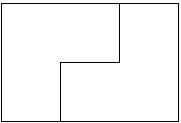
\includegraphics[angle=90]{figures/2x3tiled} 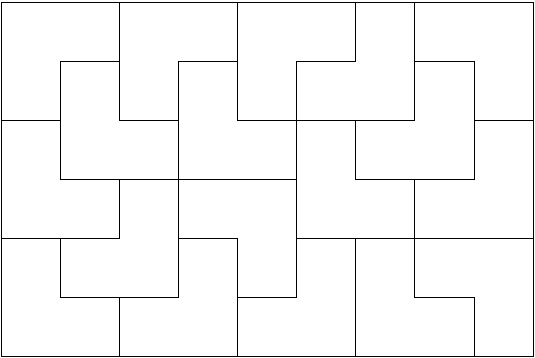
\includegraphics{figures/6x9tiled}
\end{figure}
 Lihat Gambar \ref{fig:recursion1}. Jika $n$ adalah bilangan bulat
positif, kisi $2^{n}\times2^{n}$ hampir dapat diubin seluruhnya dengan
tromino. Semua persegi kecuali satu dapat ditutupi. Cobalah, mula-mula
dengan kisi $2\times2$. Yang ini tidak terlalu sulit. Kemudian cobalah
dengan kisi $4\times4$ atau kisi $8\times8$.

Bagaimana dengan kisi $1024\times1024$? Saya tidak menyarankan Anda
benar-benar menyiapkan kisi $1024\times1024$ lalu mulai mengisinya
dengan tromino. Anda akan memerlukan $349,525$ tromino. Anda mungkin
tidak akan menyelesaikannya seumur hidup! Sebagai gantinya, sekarang
saatnya mulai berpikir secara rekursif. Gunakan hasil sebelumnya dalam
jawaban Anda. Seperti ketika Anda cukup mengatakan bahwa kantong kelereng
``berisi satu lebih banyak daripada sebelumnya'', kita dapat menyatakan
solusi pengubinan kisi $1024\times1024$ berdasarkan pengubinan kisi
$512\times512$. Caranya sebagai berikut. Ambil kisi $1024\times1024$
dan bagi menjadi empat subkisi $512\times512$ dengan membelahnya
di tengah secara horizontal dan vertikal. Pada kisi $512\times512$
di kiri atas, ubin semua persegi kecuali sudut kanan bawah. Pada kisi
$512\times512$ di kiri bawah, ubin semua persegi kecuali sudut kanan
atas. Pada kisi kanan bawah, ubin semua persegi kecuali sudut kiri
atas. Terakhir, pada kisi $512\times512$ di kanan atas, ubin semua
persegi kecuali sudut kanan atas 
\begin{figure}
\caption{\label{fig:recursion2} Kisi $2^{n}\times2^{n}$ dapat (hampir) diubin
secara rekursif.}

\centering{}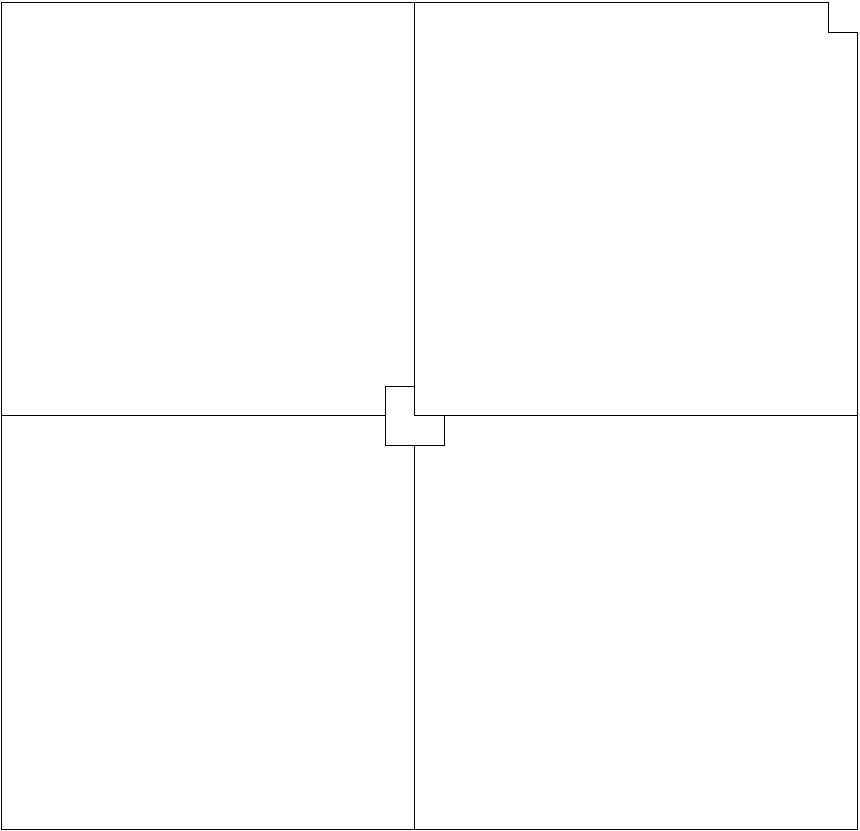
\includegraphics[scale=0.5]{figures/recursiveTiling}
\end{figure}
(Gambar \ref{fig:recursion2}). Hal ini menyisakan ruang untuk satu
tromino berbentuk L di tengah dan satu persegi yang tidak tertutupi.
Selesai! Cara ini mungkin terasa sedikit curang karena kita tidak
menjelaskan cara menangani kisi $512\times512$; namun, argumen yang
sama berlaku untuk kisi $512\times512$. Anda dapat membaginya menjadi
empat subkisi, mengubin semuanya, dan selesai.

Argumen pengubinan yang sama dapat diterapkan pada setiap kisi $2^{n}\times2^{n}$
berdasarkan pengubinan kisi $2^{n-1}\times2^{n-1}$, kecuali ketika
$n=1$. Anda hanya perlu mengubin sendiri kisi $2\times2$! Setelah
itu selesai, Anda memperoleh solusi lengkap untuk setiap kisi $2^{n}\times2^{n}$.
\begin{figure}
\caption{\label{fig:recursion3} Kisi $32\times32$ yang diubin secara rekursif.}

\centering{}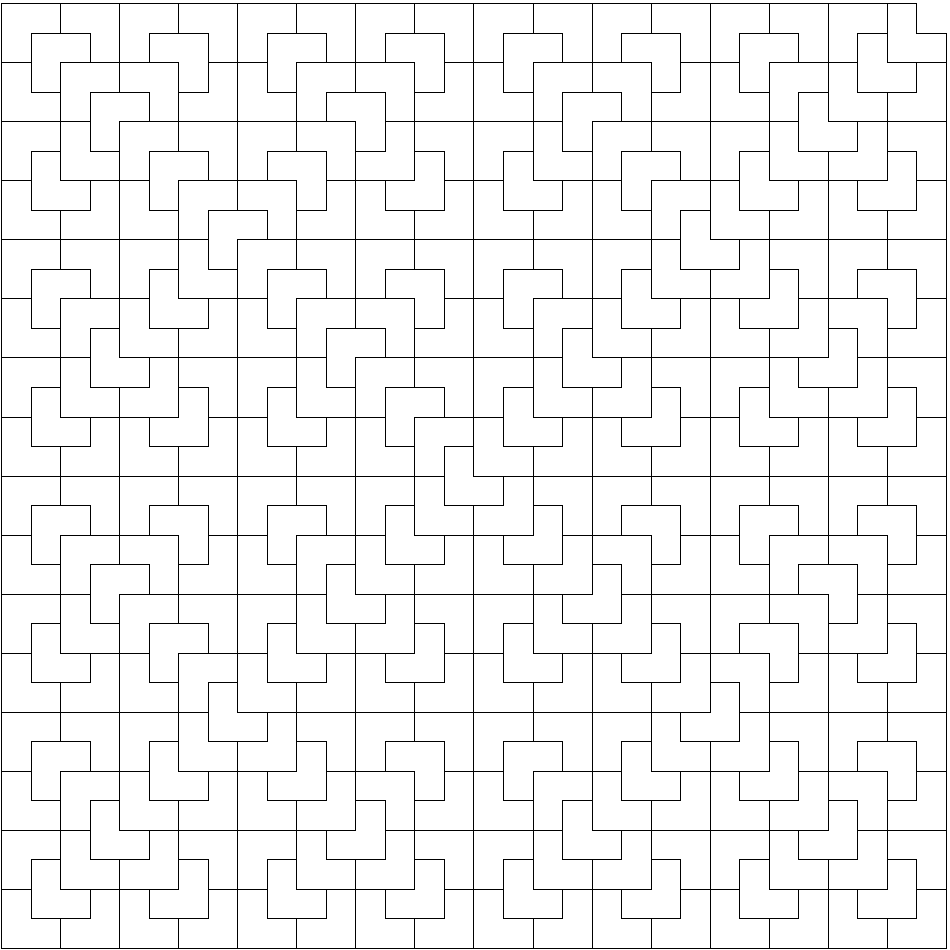
\includegraphics[scale=0.5]{figures/32x32recursive}
\end{figure}
Pengecualian serupa berlaku bagi setiap prosedur rekursif. Rekursi
hanya berguna pada hampir semua tahap. Pada suatu titik, Anda harus
turun tangan dan memberikan solusi atau jawaban. Jawaban semacam itu
sering disebut kondisi awal.

\begin{digression}{Pembuktian dengan induksi} 

\noindent Pembuktian dengan induksi juga menggunakan semacam cara
berpikir rekursif. Dalam metode ini, kita harus membuktikan bahwa
suatu klaim benar untuk suatu nilai variabel. Bagian ini serupa dengan
memiliki kondisi awal. Selanjutnya, harus dibuktikan bahwa kebenaran
klaim untuk nilai $n$ mengakibatkan kebenaran klaim untuk $n+1$.
Hal ini serupa dengan hubungan rekursif antarkeadaan. Bahkan, konstruksi
pengubinan kisi $2^{n}\times2^{n}$ berdasarkan kisi $2^{n-1}\times2^{n-1}$
ditambah pengubinan kisi $2\times2$ yang baru saja disajikan pada
dasarnya membentuk pembuktian dengan induksi bahwa kisi $2^{n}\times2^{n}$,
kecuali satu sudutnya, dapat diubin dengan tromino untuk setiap $n\geq1$.
Dengan demikian, semua pembuktian dengan induksi pada akhirnya bergantung
pada kemampuan melihat hubungan rekursif antarkeadaan.

Pada tahun 1954, Solomon Golomb \index{Golomb!Solomon} menerbitkan
pembuktian dengan induksi bahwa kisi $2^{n}\times2^{n}$ yang kehilangan
satu persegi \textit{sembarang} (tidak harus petak sudut), yang disebut
persegi defisien, dapat diubin dengan tromino. Dapatkah Anda menyusun
pengubinan (rekursif) untuk persegi defisien $2^{n}\times2^{n}$?
Dalam konstruksi tersebut, Anda dapat menggunakan pengubinan kisi
$2^{k}\times2^{k}$ yang dikurangi satu sudut.
\begin{description}
\item [{Referensi}] \cite{golomb}
\end{description}
\end{digression}

\subsection{Octave}

\subsubsection{Fungsi buatan sendiri\index{Octave!fungsi buatan sendiri}}

Seperti bahasa pemrograman modern yang berguna pada umumnya, Octave
memungkinkan kita membuat fungsi sendiri, tidak hanya fungsi yang
dapat ditulis sebagai rumus satu baris seperti fungsi anonim. Misalkan
Anda ingin menentukan nilai maksimum suatu fungsi pada sekumpulan
nilai yang berjarak sama. Fungsi itu memiliki tujuan yang sangat khusus
dan jarang digunakan. Oleh karena itu, fungsi tersebut tidak tersedia
sebagai bawaan dalam bahasa pemrograman mana pun; jika benar-benar
menginginkannya, Anda perlu menulisnya sendiri. Demikian pula, jika
Anda menginginkan fungsi yang menghitung titik simedian suatu segitiga,
Anda perlu menulisnya. Bahkan, hampir semua komputasi di luar evaluasi
fungsi dasar tidak tersedia sebagai bawaan di Octave.

Fungsi buatan sendiri ditulis berdasarkan tiga informasi pokok: nama
fungsi, daftar masukan, dan uraian keluaran. Ketiganya harus ditetapkan
dengan jelas sebelum fungsi mulai ditulis. Untuk menulis fungsi, kita
hanya perlu memberi tahu Octave nama dan masukan yang diinginkan serta
cara menentukan keluarannya. Format dasar suatu fungsi adalah sebagai
berikut:\begin{verbatim}
function ans = myName(input1, input2, ... )
  ...
  ans = final answer;
end%function
\end{verbatim}Baris pertama memuat nama fungsi dan daftar masukan. Bagian fungsi
lainnya digunakan untuk menghitung keluaran, \texttt{ans}.

Fungsi yang menentukan nilai maksimum suatu fungsi pada sekumpulan
nilai yang berjarak sama dapat ditulis melalui langkah-langkah berikut.
Pertama, kita memutuskan untuk menamainya ``maxOverMesh''. Perhatikan
bahwa nama tersebut tidak mengandung spasi atau karakter khusus. Hanya
sedikit karakter nonalfabet yang dapat digunakan dalam nama fungsi.
Biasanya tanda garis bawah dan angka aman digunakan, tetapi karakter
lain belum tentu dapat digunakan! Sebaiknya batasi diri pada karakter
tersebut. Kedua, kita perlu memikirkan masukan yang diperlukan fungsi
ini. Tentu saja, fungsi yang akan dimaksimumkan diperlukan, dan kisi
titik tempat fungsi itu diperiksa juga harus ditentukan. Ada beberapa
cara untuk melakukannya, tetapi cara yang mungkin paling mudah bagi
pengguna ialah meminta titik ujung bawah, titik ujung atas, dan jumlah
interval pada kisi. Terakhir, kita perlu menulis kode yang menerima
masukan tersebut dan menentukan nilai maksimum fungsi pada kisi. Salah
satu caranya adalah sebagai berikut: \begin{verbatim}
%%%%%%%%%%%%%%%%%%%%%%%%%%%%%%%%%%%%%%%%%%%%%%%%%%%%%%%%%%%
%  maxOverMesh() written by Leon Q. Brin 21 January 2013  %
%  INPUT: Interval [a,b]; function f; and number of       %
%         subintervals n.                                 %
%  OUTPUT: maximum value of the function over the end     %
%         points of the subintervals.                     %
%%%%%%%%%%%%%%%%%%%%%%%%%%%%%%%%%%%%%%%%%%%%%%%%%%%%%%%%%%% 
function ans = maxOverMesh(f,a,b,n)
  ans = f(a);
  for i=1:n
    x = (i*b + (n-i)*a)/n;
    F = f(x);
    if (F>ans) ans = F;
  end%for
end%function
\end{verbatim}Merupakan praktik yang baik untuk mengawali setiap fungsi yang Anda
tulis dengan komentar berisi uraian tiga hal tentang fungsi tersebut---nama,
masukan, dan keluaran. Jika kelak Anda atau orang lain membacanya,
tersedia ringkasan singkat tentang cara dan tujuan penggunaan fungsi
tersebut.

Nilai yang disimpan dalam \texttt{ans} saat fungsi selesai menjadi
keluaran fungsi. Pada awalnya, \texttt{ans} diisi dengan nilai fungsi
di titik ujung kiri. Selanjutnya, fungsi melakukan perulangan melalui
titik-titik ujung subselang lainnya dan menghitung nilai fungsi pada
setiap titik. Setiap kali menemukan nilai yang lebih besar daripada
\texttt{ans}, fungsi memperbarui nilai \texttt{ans} dengan nilai tersebut.
Pada akhir perulangan, \texttt{ans} berisi nilai terbesar fungsi.

Untuk menggunakan fungsi buatan sendiri, simpan fungsi tersebut dalam
berkas \texttt{.m} \index{Octave!berkas .m@berkas \texttt{.m}} dengan
nama yang sama dengan nama fungsi. Sebagai contoh, fungsi \texttt{maxOverMesh()}
akan disimpan dalam berkas bernama \texttt{maxOverMesh.m}. Setelah
itu, fungsi buatan sendiri dapat dipanggil seperti fungsi bawaan Octave
mana pun, asalkan berkas \texttt{.m} dan program yang menggunakannya
disimpan dalam direktori yang sama. Jika fungsi digunakan dari baris
perintah, direktori kerja Octave (direktori tempat Octave dijalankan,
kecuali diubah secara eksplisit selama sesi) harus merupakan direktori
tempat berkas \texttt{.m} disimpan:\begin{verbatim}
octave:1> maxOverMesh(@(x) (x^2-6*x+8)*exp(x), 0, 4, 99)
ans =  8.6728
octave:2> f = @(x) (x^2+3*x-5)/(x^2-3*x+5)
f =
@(x) (x ^ 2 + 3 * x - 5) / (x ^ 2 - 3 * x + 5)
octave:3> maxOverMesh(f, -5, 5, 225)
ans =  2.6362
\end{verbatim}\texttt{maxOverMesh.m} dapat diunduh dari \href{http://lqbrin.github.io/tea-time-numerical/ancillaries.html}{situs pendamping}.

\subsubsection{Fungsi rekursif}

Dengan berpikir secara rekursif, apa jawaban Anda jika saya menanyakan
nilai $10!$? Renungkan sejenak sebelum melanjutkan. Betul! 10 faktorial
hanyalah 10 dikalikan $9!$:
\begin{eqnarray*}
10! & = & 10\cdot9\cdot8\cdot7\cdot6\cdot5\cdot4\cdot3\cdot2\cdot1\\
 & = & 10\cdot(9\cdot8\cdot7\cdot6\cdot5\cdot4\cdot3\cdot2\cdot1)\\
 & = & 10\cdot(9!).
\end{eqnarray*}
Tidak perlu memperoleh sebuah bilangan. Cukup gunakan gagasan rekursif,
sebab gagasan itu tentu sama berlakunya untuk $9!$, dan seterusnya
$\ldots$ hingga (atau mungkin seharusnya saya katakan menurun hingga?)
suatu titik. Pada titik apa pernyataan $n!=n\cdot(n-1)!$ tidak lagi
benar? Ketika $n=0$. Kita perlu menetapkan bahwa $0!=1$ dan tidak
mengandalkan pemikiran rekursif dalam kasus ini. Namun, hanya dalam
kasus ini!

Mari kita lihat bagaimana perhitungan rekursif ini bekerja untuk $5!$.
Menurut rekursi tersebut, $5!=5\cdot4!$. Namun, $4!=4\cdot3!$ sehingga
diperoleh $5!=5\cdot(4\cdot3!)$. Namun, $3!=3\cdot2!$ sehingga sekarang
diperoleh $5!=5(4(3\cdot2!))$. Dengan melanjutkan proses ini, $2!=2\cdot1!=2\cdot1\cdot0!$
sehingga sekarang diperoleh $5!=5(4(3(2(1\cdot0!))))$. Sekarang rekursi
berhenti dan kita cukup menyubstitusikan 1 untuk $0!$ sehingga diperoleh
$5!=5(4(3(2(1(1)))))$. Mungkin Anda mengharapkan $5\cdot4\cdot3\cdot2\cdot1$
sebagai hasil akhirnya. Tentu saja, kedua cara tersebut sama-sama
menghasilkan 120, sehingga dari segi ketepatan, keduanya tidak bermasalah.
Secara praktis, perbedaannya tidak berarti. Menghitung faktorial secara
rekursif amat tidak efisien dan mustahil dilakukan melampaui kedalaman
rekursi maksimum bahasa pemrograman yang digunakan, sehingga cara
ini tidak boleh dipakai dalam praktik. Satu-satunya manfaatnya adalah
sebagai latihan berpikir dan memprogram secara rekursif.

Secara umum, fungsi rekursif \index{Octave!fungsi rekursif} akan
tampak seperti berikut:\begin{verbatim}
function ans = recFunction(input1, input2, ... )
  if (recursion does not apply)
    return appropriate ans
  else
    return recFunction(i1, i2, ... )
  end%if
end%function
\end{verbatim}Hal pertama yang perlu dilakukan adalah menentukan apakah rekursi
berlaku. Jika tidak, keluaran yang sesuai harus diberikan. Jika ya,
fungsi rekursif cukup memanggil dirinya sendiri dengan masukan yang
telah diubah. Karena definisi rekursif (yang agak usil) untuk $n!$
adalah $n\cdot(n-1)!$ dan berlaku setiap kali $n>0$, sedangkan $0!=1$,
fungsi faktorial rekursif dapat tampak seperti berikut:\begin{verbatim}
%%%%%%%%%%%%%%%%%%%%%%%%%%%%%%%%%%%%%%%%%%%%%%%%%%%%%%%%%%%%
%  recFactorial() written by Leon Q. Brin 21 January 2013  %
%       is a recursively defined factorial function.       %
%  INPUT: nonnegative integer n.                           %
%  OUTPUT: n!                                              %
%%%%%%%%%%%%%%%%%%%%%%%%%%%%%%%%%%%%%%%%%%%%%%%%%%%%%%%%%%%%
function ans = recFactorial(n)
  if (n==0)
    ans = 1;
  else
    ans = n*recFactorial(n-1);
  end%if
end%function
\end{verbatim}

\noindent Perhatikan \texttt{==} ketika memeriksa apakah \texttt{n}
sama dengan \texttt{1}. Ini bukan kesalahan ketik. Hal ini sangat
penting. Semua bahasa pemrograman harus membedakan penugasan dan kondisi.
Di atas kertas, menuliskan $x=3$ ketika Anda ingin menetapkan $x$
sama dengan 3 mungkin terasa wajar. Menuliskan ``jika $x=3$, semuanya
baik-baik saja'' juga mungkin terasa wajar. Kita menggunakan ``persamaan''
$x=3$ dengan cara yang persis sama di atas kertas untuk menyatakan
dua hal yang sangat berbeda. Ketika kita menetapkan $x=3$ kita membuat
sebuah pernyataan, atau melakukan penugasan nilai 3 kepada variabel
$x$. Namun, ketika kita menulis ``jika $x=3\ldots$'' kita membuat
pernyataan hipotetis, atau pernyataan kondisional. Nilai $x$ belum
diketahui. Dalam Octave, keduanya dibedakan dengan menggunakan satu
tanda sama dengan, \texttt{=}, untuk menyatakan penugasan dan dua
tanda sama dengan, \texttt{==}, untuk menguji kesamaan. Operator perbandingan
lain yang mungkin Anda perlukan adalah \texttt{<} dan \texttt{>},
yang memiliki arti sebagaimana lazimnya, serta \texttt{<=} dan \texttt{>=}
yang masing-masing berarti $\leq$ dan $\geq$, secara berurutan.
\texttt{recFactorial.m} dapat diunduh dari \href{http://lqbrin.github.io/tea-time-numerical/ancillaries.html}{situs pendamping}.

\noindent\startexercises

\subsection{Latihan}
\begin{enumerate}
\item \octave\ Tulislah berkas .m dengan sebuah fungsi yang menerima satu
masukan, menguadratkannya, dan mengembalikan hasilnya. Berkas Anda
harus

\begin{enumerate}
\item memuat blok komentar di bagian awal yang berisi nama Anda, tanggal,
serta penjelasan mengenai apa yang dilakukan program tersebut dan
cara menggunakannya.
\item memuat fungsi berbentuk \texttt{foo(x)} yang mengembalikan kuadrat
dari masukan (argumen) \texttt{x}.
\end{enumerate}
Pastikan Anda menguji fungsi tersebut melalui baris perintah Octave.
\item \octave\ Fungsi Octave \texttt{foo(x)} ditampilkan di bawah ini.

\begin{verbatim}
function res = foo(x)
  if (x<1)
    res = 0;
  else
    half = x/2;
    floorhalf = floor(half);
    if (half == floorhalf)
      res = 0 + foo(floorhalf);
    else
      res = 1 + foo(floorhalf);
    end%if
  end%if
end%function
\end{verbatim}
\begin{enumerate}
\item Hitung \texttt{foo(2)}.
\item Hitung \texttt{foo(23)}.
\end{enumerate}
\item \octave\ Tulislah fungsi Octave rekursif yang menghitung 
\[
\sum_{i=1}^{n}\frac{1}{i}
\]
\item \octave\ Tulislah fungsi Octave rekursif yang menghitung $a_{n}$
untuk setiap $n\geq0$, dengan ketentuan
\begin{eqnarray*}
a_{0} & = & 100,000\\
a_{n} & = & 1.05a_{n-1}-1200,\quad n>0.
\end{eqnarray*}
\item \label{recursive1}Barisan Fibonacci, $\left\langle F_{n}\right\rangle $,
didefinisikan secara rekursif oleh
\begin{align*}
F_{n+1} & =F_{n}+F_{n-1},\quad n\geq1\\
F_{0} & =1\\
F_{1} & =1
\end{align*}
sehingga beberapa suku pertamanya adalah $1,1,2,3,5,8$. 

\begin{enumerate}
\item \label{recursiveFib}Tulislah fungsi rekursif yang menghitung suku
$n$ dalam barisan Fibonacci. Fungsi Anda harus memiliki satu argumen,
$n$. 
\item \label{forloopFib}Tulislah fungsi yang menggunakan perulangan for
untuk menghitung suku $n$ dalam barisan Fibonacci. Fungsi Anda harus
memiliki satu argumen, $n$. 
\item Tulislah program yang memanggil fungsi dari \ref{recursiveFib} untuk
menghitung $F_{30}$.
\item Tulislah program yang memanggil fungsi dari \ref{forloopFib} untuk
menghitung $F_{30}$.
\item Kode manakah yang lebih sederhana (rekursif atau nonrekursif)?
\item Kode manakah yang lebih cepat?
\item Kode manakah yang lebih akurat?
\end{enumerate}
\textbf{CATATAN}: $F_{30}=1346269$.
\item \label{recursive2}Misalkan barisan $\left\langle a_{n}\right\rangle $
didefinisikan oleh 
\begin{align*}
a_{n+1} & =\frac{1}{4}\left|5a_{n}^{2}-30a_{n}+25\right|,\quad n\geq1\\
a_{0} & =\frac{17+2\sqrt{7}}{5}.
\end{align*}

\begin{enumerate}
\item Hitung $a_{1},a_{2}$ dan $a_{3}$ secara eksak.
\item Tentukan $a_{20}$ dan $a_{51}$ secara eksak.
\item Tulislah fungsi rekursif yang menghitung suku $n$ dari barisan tersebut.
Fungsi Anda harus memiliki satu argumen, $n$. Tulislah program yang
memanggil fungsi ini untuk menghitung $a_{1},a_{2},a_{3},a_{20},$
dan $a_{51}$.
\item Tulislah fungsi yang menggunakan perulangan for untuk menghitung suku
$n$ dari barisan tersebut. Fungsi Anda harus memiliki satu argumen,
$n$. Tulislah program yang memanggil fungsi ini untuk menghitung
$a_{1},a_{2},a_{3},a_{20},$ dan $a_{51}$.
\item Kode manakah yang lebih sederhana (rekursif atau nonrekursif)?
\item Fungsi manakah yang lebih cepat?
\item Kode manakah yang lebih akurat, dan mengapa?
\item Fungsi manakah yang lebih baik, dan mengapa?
\item Apakah Anda yakin salah satu dari kedua fungsi tersebut dapat menghitung
$a_{600}$ secara akurat? Jika tidak, mengapa?
\end{enumerate}
\item \label{exc:recursion}Tromino, bagian 1. \hasananswer 

\begin{enumerate}
\item Dengan pendekatan rekursif, berapa banyak tromino yang diperlukan
untuk mengubin kisi $2^{n}\times2^{n}$ dengan menyisakan satu persegi
di sudut?
\item \label{tromino-greatest}Berapa nilai bilangan bulat terbesar untuk
$n$ yang tidak tercakup dalam definisi rekursif tersebut?
\item Untuk nilai $n$ pada bagian \ref{tromino-greatest}, berapa banyak
tromino yang diperlukan?
\end{enumerate}
\item \label{exc:recursion-1}\octave\ Tromino, bagian 2. \hasasolution 

\begin{enumerate}
\item Tulislah fungsi Octave rekursif untuk menghitung banyaknya tromino
yang diperlukan untuk mengubin kisi $2^{n}\times2^{n}$ dengan menyisakan
satu persegi di sudut.
\item Gunakan fungsi Anda untuk memverifikasi bahwa sebanyak $349,525$
tromino diperlukan untuk mengubin kisi $1024\times1024$ dengan menyisakan
satu persegi di sudut.
\end{enumerate}
\item \label{exc:recursion-2}Menara Hanoi, bagian 1. Menara Hanoi adalah
permainan yang menggunakan sejumlah cakram dengan ukuran berbeda-beda,
yang ditumpuk pada sebuah tiang dari yang terbesar di bawah hingga
yang terkecil di atas. Terdapat dua tiang lain yang pada awalnya kosong.
Tujuannya adalah memindahkan seluruh tumpukan cakram ke salah satu
tiang yang semula kosong dengan mengikuti dua aturan. Anda hanya boleh
memindahkan satu cakram pada satu waktu dari satu tiang ke tiang lain.
Anda tidak boleh meletakkan cakram di atas cakram yang lebih kecil. \hasasolution 

\begin{enumerate}
\item Dengan memulai dari tumpukan tiga cakram, berapakah jumlah langkah
minimum yang diperlukan untuk menyelesaikan permainan? Jawablah pertanyaan
ini dengan sebuah bilangan.
\item Dengan memulai dari tumpukan empat cakram, berapakah jumlah langkah
minimum yang diperlukan untuk menyelesaikan permainan?

\begin{enumerate}
\item \label{enu:tower-recursion}Jawablah pertanyaan ini secara rekursif.
\item Berdasarkan jawaban rekursif Anda, jawablah pertanyaan ini dengan
sebuah bilangan.
\end{enumerate}
\end{enumerate}
\item \label{exc:recursion-3}Menara Hanoi, bagian 2. \hasasolution 

\begin{enumerate}
\item Dengan memulai dari sebuah ``tumpukan'' yang hanya terdiri dari
satu cakram, berapakah jumlah langkah minimum yang diperlukan untuk
menyelesaikan permainan?
\item \octave\ Gunakan jawaban Anda untuk bagian (a), bersama generalisasi
jawaban Anda atas soal  \ref{enu:tower-recursion} untuk menulis fungsi
Octave rekursif yang menghitung jumlah langkah minimum yang diperlukan
untuk menyelesaikan permainan dengan tumpukan $n$ cakram.
\item \octave\ Gunakan fungsi Octave Anda untuk memverifikasi bahwa jumlah
langkah minimum untuk menyelesaikan permainan dengan tumpukan 10 cakram
adalah 1023.
\end{enumerate}
\item Menara Hanoi, bagian 3. Menara Hanoi dengan syarat ketetanggaan. Misalkan
aturan Menara Hanoi diubah sehingga setiap cakram hanya boleh dipindahkan
ke tiang yang bersebelahan, dan tujuannya adalah memindahkan seluruh
tumpukan dari tiang paling kiri ke tiang paling kanan.

\begin{enumerate}
\item Berapa jumlah langkah minimum yang diperlukan untuk menyelesaikan
permainan dengan sebuah  ``tumpukan'' yang terdiri atas satu cakram?
\item Tentukan rumus rekurensi untuk jumlah langkah minimum yang diperlukan
untuk menyelesaikan permainan dengan tumpukan $n$ cakram, $n>1$.
\item \octave\ Tulislah fungsi Octave rekursif yang menghitung jumlah langkah
minimum untuk menyelesaikan permainan dengan tumpukan $n$ cakram.
\item \octave\ Gunakan fungsi Octave Anda untuk menghitung jumlah langkah
minimum yang diperlukan untuk menyelesaikan permainan dengan tumpukan
$5$ cakram dan  $10$ cakram.
\end{enumerate}
\item Bilangan Stirling jenis kedua, bagian 1. Misalkan $S(n,k)$ menyatakan
banyaknya cara mempartisi suatu himpunan yang terdiri atas $n$ elemen
menjadi $k$ subhimpunan tak kosong. Partisi atas suatu himpunan $A$
adalah koleksi subhimpunan dari $A$ sedemikian sehingga setiap elemen
himpunan $A$ menjadi anggota tepat satu subhimpunan tersebut. Urutan
subhimpunan tidak berpengaruh karena partisi merupakan suatu koleksi
(himpunan yang anggotanya juga berupa himpunan). Sebagai contoh, partisi
$\{\{1\},\{2,3\},\{4\}\}$ merupakan partisi atas $\{1,2,3,4\}$.
$\{\{4\},\{1\},\{2,3\}\}$ merupakan partisi yang sama atas $\{1,2,3,4\}$.

\begin{enumerate}
\item \label{exc:recursion-4}Tentukan $S(10,1)$. \hasasolution 
\item Tentukan $S(3,2)$.
\item Tentukan $S(4,3)$.
\item \label{exc:recursion-5}Tentukan $S(4,2)$. \hasasolution 
\item Tentukan $S(8,8)$.
\end{enumerate}
\item \label{exc:recursion-6}\label{enu:Stirling2}Bilangan Stirling jenis
kedua, bagian 2.  \hasasolution 

\begin{enumerate}
\item Tentukan $S(n,1)$.
\item Tentukan $S(n,n)$.
\end{enumerate}
\item \label{exc:recursion-7}\label{enu:Stirling3}Bilangan Stirling jenis
kedua, bagian 3. Misalkan $A=\{1,2,3,\ldots,n\}$. \hasananswer 

\begin{enumerate}
\item Berapa banyak partisi atas $A$ menjadi $k$ subhimpunan tak kosong
yang memuat subhimpunan $\{n\}$? Nyatakan jawaban Anda dalam bentuk
bilangan Stirling jenis kedua.
\item Berapa banyak partisi atas $A$ menjadi $k$ subhimpunan tak kosong
yang tidak memuat subhimpunan $\{n\}$? Nyatakan jawaban Anda dalam
bentuk bilangan Stirling jenis kedua. Petunjuk: pertimbangkan partisi
atas $B=\{1,2,3,\ldots,n-1\}$ menjadi $k$ subhimpunan tak kosong.
\end{enumerate}
\item Bilangan Stirling jenis kedua, bagian 4.

\begin{enumerate}
\item Gunakan jawaban Anda untuk soal \ref{enu:Stirling2} dan \ref{enu:Stirling3}
guna menurunkan rumus rekurensi beserta syarat awal bagi banyaknya
cara suatu himpunan yang terdiri atas $n$ elemen dapat dipartisi
menjadi $k$ subhimpunan.
\item \octave\ Tulislah fungsi Octave rekursif yang menghitung bilangan
Stirling jenis kedua.
\item \octave\ Gunakan fungsi Octave Anda untuk memverifikasi bahwa $S(10,4)=34105$.
\end{enumerate}
\item \label{exc:recursion-8}Sekumpulan balok terdiri atas beberapa balok
setinggi 1 inci dan beberapa balok setinggi 2 inci. Ada berapa cara
untuk membentuk tumpukan balok setinggi $15$ inci? \hasasolution 
\item Seekor lebah jantan hanya memiliki satu induk karena lebah jantan
berasal dari telur ratu lebah yang tidak dibuahi. Seekor lebah betina
(ratu lebah) memiliki dua induk. Jadi, jika ditelusuri 0 generasi
ke belakang, seekor lebah jantan memiliki satu leluhur (lebah itu
sendiri). Jika ditelusuri 1 generasi ke belakang, lebah itu juga memiliki
1 leluhur (induk betinanya). Jika ditelusuri 2 generasi ke belakang,
lebah itu memiliki 2 leluhur (kedua induk dari induk betinanya). Berapa
banyak leluhur langsung yang dimiliki seekor lebah jantan jika ditelusuri
$n$ generasi ke belakang?
\item Berikan argumen bahwa setiap poligon dapat ditriangulasi (ditutupi
oleh segitiga-segitiga yang tidak saling tumpang tindih). Berikut
ini contoh triangulasi sebuah dodekagon.

\begin{center}
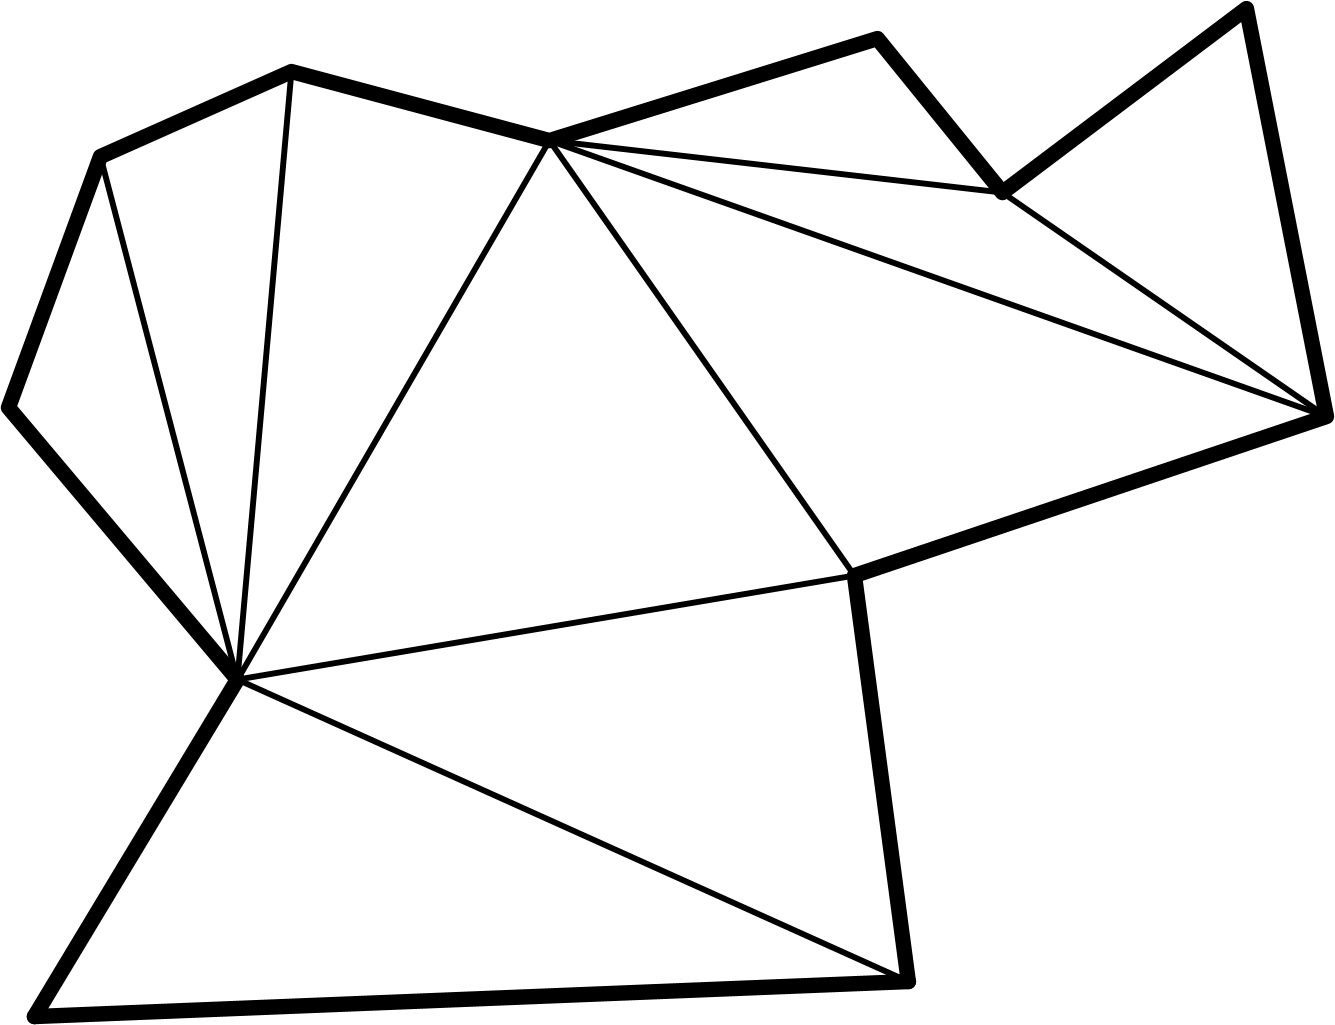
\includegraphics[scale=0.25]{figures/triangulation}
\par\end{center}
\item Pada soal \ref{recursive1} dan \ref{recursive2}, Anda seharusnya
memperhatikan bahwa fungsi-fungsi rekursif lebih lambat daripada padanannya
yang menggunakan perulangan for. Berapa kali lebih lambat? Mengapa
rekursi Fibonacci jauh lebih lambat daripada padanannya yang menggunakan
perulangan for?
\item Misalkan barisan $\left\langle b_{n}\right\rangle $ dan $\left\langle c_{n}\right\rangle $
didefinisikan sebagai berikut.
\begin{eqnarray*}
b_{0} & = & \frac{1}{3};\quad b_{n+1}=4b_{n}-1,\quad n\geq0\\
c_{0} & = & \frac{1}{10};\quad c_{n+1}=4c_{n}(1-c_{n}),\quad n\geq0
\end{eqnarray*}

\begin{enumerate}
\item Tulislah fungsi yang menggunakan perulangan for untuk menghitung suku
$n$ dari barisan $\left\langle b_{n}\right\rangle $. Fungsi Anda
harus memiliki satu argumen, $n$.
\item Tulislah fungsi yang menggunakan perulangan for untuk menghitung suku
$n$ dari barisan $\left\langle c_{n}\right\rangle $. Fungsi Anda
harus memiliki satu argumen, $n$.
\item Tulislah program yang memanggil fungsi Anda dari bagian (a) untuk
menghitung $b_{30}$. Seberapa akurat hasil perhitungan ini? PETUNJUK:
$b_{30}=\frac{1}{3}$. 
\item Tulislah program yang memanggil fungsi Anda dari bagian (b) untuk
menghitung $c_{50}$. Seberapa akurat hasil perhitungan ini? PETUNJUK:
$c_{50}=.5392$, akurat hingga 4 tempat desimal.
\item Dapatkah Anda menemukan cara untuk membuat perhitungan ini lebih andal
(lebih akurat)?
\end{enumerate}
\end{enumerate}
\finishexercises 


% Chapter 2 -- Root Finding 


\chapter{Pencarian Akar}

\section{Metode Bagi Dua\label{sec:Bisection}\index{metode bagi dua}\index{metode!bagi dua|see {metode bagi dua}}}

Pada Bagian \ref{sec:Taylor} (halaman \pageref{equationToSolve}),
kita menyatakan bahwa ``$T_{2}(x)$ sebenarnya menghampiri $\ln(x)$
dengan selisih tidak lebih dari $0.1$ pada interval $[3.296,13.13]$'',
seraya berjanji akan membahas perhitungannya nanti. Sekaranglah saatnya.
Pertama-tama, kita nyatakan kembali klaim tersebut sebagai ``jarak
antara $T_{2}(x)$ dan $\ln(x)$ kurang dari atau sama dengan $0.1$
untuk setiap $x\in[3.296,13.13]$.'' Dengan kata lain, 
\[
|T_{2}(x)-\ln(x)|<\frac{1}{10}\quad\mbox{untuk setiap }x\in[3.296,13.13].
\]
Salah satu cara untuk mulai menyelesaikan pertidaksamaan ini adalah
mempertimbangkan pasangan persamaan $T_{2}(x)-\ln(x)=\pm\frac{1}{10}$.
Dengan berfokus pada penyelesaian 
\begin{equation}
T_{2}(x)-\ln(x)=\frac{1}{10},\label{eq:bisectionExample}
\end{equation}
ingat bahwa $T_{2}(x)=2+\frac{x-e^{2}}{e^{2}}-\frac{(x-e^{2})^{2}}{2e^{4}}$.
Jadi, kita hendak menyelesaikan persamaan
\[
2+\frac{x-e^{2}}{e^{2}}-\frac{(x-e^{2})^{2}}{2e^{4}}-\ln(x)=\frac{1}{10}.
\]
Akhirnya, setelah menuliskan persamaan secara lengkap, tidak mengherankan
bahwa kita tidak akan menyelesaikannya untuk $x$ secara eksak. Tidak
ada metode analitik untuk menyelesaikan persamaan semacam itu. Secara
umum, persamaan yang memuat suku polinomial sekaligus suku transendental
tidak dapat diselesaikan secara analitik. Namun, dari grafik pada
Gambar \ref{fig:taylor3}, kita dapat memperoleh hampiran awal bagi
solusinya. Kita mencari titik tempat $T_{2}(x)$ melebihi $\ln(x)$
sebesar $0.1$. Karena kedua grafik hampir berimpit pada $x=6$, kita
dapat menduga bahwa $T_{2}(6)$ melebihi $\ln(x)$ sebesar \textit{kurang
dari} $0.1$ di sana. Karena terdapat celah yang cukup besar antara
kedua grafik pada $x=2$, kita juga dapat menduga bahwa $T_{2}(2)$
melebihi $\ln(x)$ sebesar \textit{lebih dari} $0.1$ di sana. Dengan
kata lain, $T_{2}(2)-\ln(2)>\frac{1}{10}$ sedangkan $T_{2}(6)-\ln(6)<\frac{1}{10}$.
Karena $T_{2}(x)-\ln(x)$ kontinu pada interval $[2,6]$, teorema
nilai antara menjamin adanya nilai $c\in(2,6)$ sedemikian rupa sehingga
$T_{2}(c)-\ln(c)=\frac{1}{10}$. Nilai $c$ inilah yang kita cari.
Kita sudah tahu bahwa nilainya berada di antara 2 dan 6. Ini baru
permulaan, tetapi kita dapat memperoleh hasil yang lebih baik!

Bagaimana dengan 4? Nah, $T_{2}(4)-\ln(4)\approx.04986<0.1$, sehingga
sekarang kita tahu bahwa $T_{2}(4)$ melebihi $\ln(4)$ sebesar \textit{kurang
dari} $0.1$. Sekarang teorema nilai antara memberi tahu kita bahwa
$c$ berada di antara 2 dan 4 ($T_{2}(2)$ melebihi $\ln(x)$ sebesar
\textit{lebih dari} $0.1$). Bagaimana jika kita periksa $x=3$? Mari.
$T_{2}(3)-\ln(3)\approx.131>0.1$, sehingga sekarang kita tahu bahwa
$T_{2}(3)$ melebihi $\ln(3)$ sebesar \textit{lebih dari} $0.1$.
Ringkasnya, $T_{2}(4)-\ln(4)<0.1$ sedangkan $T_{2}(3)\ln(3)>0.1$.
Sekali lagi, berdasarkan teorema nilai antara, kita tahu bahwa $c$
berada di antara 3 dan 4. Kita dapat terus mengulangi proses ini;
batasnya hanyalah kesabaran kita. Proses inilah yang kita sebut \index{metode bagi dua}metode
bagi dua:
\begin{enumerate}
\item Tentukan interval $[a,b]$ sedemikian rupa sehingga salah satu dari
$a$ atau $b$ menghasilkan nilai di atas sasaran, sedangkan yang
lain menghasilkan nilai di bawah sasaran.
\item Hitung titik tengah, $m$, dari interval tersebut.
\item Jika $a$ dan $m$ sama-sama menghasilkan nilai di atas sasaran atau
sama-sama di bawah sasaran, nilai yang dicari terletak dalam $[m,b]$.
\item Jika $b$ dan $m$ sama-sama menghasilkan nilai di atas sasaran atau
sama-sama di bawah sasaran, nilai yang dicari terletak dalam $[a,m]$.
\item Kembali ke langkah 2 dengan menggunakan interval baru tersebut.
\end{enumerate}
\begin{figure}[h]
\caption{\label{fig:bisection-1}$+$ menunjukkan $T_{2}(x)-\ln(x)>\frac{1}{10}$
dan $-$ menunjukkan $T_{2}(x)-\ln(x)<\frac{1}{10}$.}

\centering{}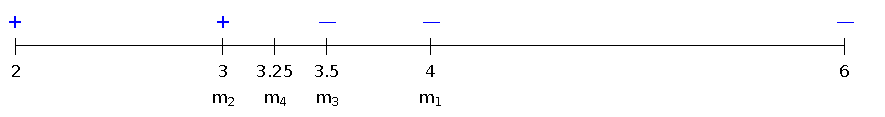
\includegraphics[width=5.5in]{figures/roots-bisection1}
\end{figure}
 Dengan menggunakan tanda $+$ untuk nilai $x$ yang membuat $T_{2}(x)-\ln(x)$
melebihi nilai sasaran $\frac{1}{10}$ dan tanda $-$ untuk nilai
$x$ yang membuat $T_{2}(x)-\ln(x)$ berada di bawah nilai sasaran
$\frac{1}{10}$, kita dapat menggambarkan prosedur ini, termasuk dua
iterasi berikutnya, seperti pada Gambar \ref{fig:bisection-1}. Kita
juga dapat menyajikan kembali perhitungannya dalam sebuah tabel:
\begin{center}
\begin{tabular}{cccccc}
$a$ & $m$ & $b$ & $T_{2}(a)-\ln(a)$ & $T_{2}(m)-\ln(m)$ & $T_{2}(b)-\ln(b)$\tabularnewline
\hline 
2 & 4 & 6 & $.3116$ & $.04986$ & $.002582$\tabularnewline
2 & 3 & 4 & $.3116$ & $0.131$ & $.04986$\tabularnewline
3 & $3.5$ & 4 & $0.131$ & $0.0824$ & $.04986$\tabularnewline
3 & $3.25$ & $3.5$ &  &  & \tabularnewline
\end{tabular}
\par\end{center}

\noindent Bagaimanapun cara kita memahami prosedur tersebut, prosedur
itu menghasilkan barisan hampiran 
\[
4,\ 3,\ 3.5,\ 3.25,\ \ldots
\]
. Berapakah nilai berikutnya? Jawaban \vpageref{subsec:bisectionAnswer1}.

Kita tidak hanya memperoleh barisan bilangan yang mendekati solusi,
tetapi juga mengetahui dengan pasti bahwa $4$ berjarak tidak lebih
dari 2 satuan dari nilai eksak. $3$ berjarak tidak lebih dari 1 satuan.
$3.5$ berjarak tidak lebih dari $0.5$ satuan. Dan $3.25$ berjarak
tidak lebih dari $0.25$ satuan. Secara umum, setiap hampiran berjarak
paling jauh setengah panjang interval tempat hampiran itu dihitung
sebagai titik tengah. Bagaimanapun, nilai eksak dijamin terletak di
dalam interval tersebut. Jarak terjauh yang mungkin antara titik tengah
dan nilai eksak adalah setengah panjang interval.

Walaupun metode ini bekerja dengan baik sebagaimana dijelaskan, biasanya
persamaan yang hendak diselesaikan disederhanakan sehingga salah satu
ruasnya bernilai nol. Dengan demikian, ruas yang lain dapat dipandang
sebagai fungsi yang akarnya dicari. Selain itu, cara ini sedikit menyederhanakan
implementasi metode. Sebagai contoh, kita akan menyelesaikan persamaan
\[
T_{2}(x)-\ln(x)-\frac{1}{10}=0
\]
bukan persamaan \ref{eq:bisectionExample}. Prosedurnya kemudian cukup
berupa pencarian akar fungsi $f(x)=T_{2}(x)-\ln(x)-\frac{1}{10}$.
Karena itulah metode ini disebut metode pencarian akar. Metode ini
digunakan untuk mencari nol, atau akar, suatu fungsi. Dari sudut pandang
ini, delapan iterasi pertama prosedur tersebut dapat diringkas sebagai
berikut:

\begin{center}
\begin{tabular}{cccccc}
$a$ & $m$ & $b$ & $f(a)$ & $f(m)$ & $f(b)$\tabularnewline
\hline 
2 & 4 & 6 & $>0$ & $<0$ & $<0$\tabularnewline
2 & 3 & 4 & $>0$ & $>0$ & $<0$\tabularnewline
3 & $3.5$ & 4 & $>0$ & $<0$ & $<0$\tabularnewline
3 & $3.25$ & $3.5$ & $>0$ & $>0$ & $<0$\tabularnewline
$3.25$ & $3.375$ & $3.5$ & $>0$ & $<0$ & $<0$\tabularnewline
$3.25$ & $3.3125$ & $3.375$ & $>0$ & $<0$ & $<0$\tabularnewline
$3.25$ & $3.28125$ & $3.3125$ & $>0$ & $>0$ & $<0$\tabularnewline
$3.28125$ & $3.296875$ & $3.3125$ &  &  & \tabularnewline
\end{tabular}
\par\end{center}

\noindent Perhatikan dua hal. Nilai sebenarnya dari $f(a)$, $f(m)$,
dan $f(b)$ tidak diperlukan. Hanya tandanya yang penting, sebab kita
hanya perlu mempertahankan satu titik ujung tempat fungsi bernilai
lebih besar daripada 0 (di atas sasaran) dan satu titik ujung tempat
fungsi bernilai kurang daripada 0 (di bawah sasaran). Selain itu,
kolom $f(a)$ dan $f(b)$ sebenarnya juga tidak mutlak diperlukan.
Jika prosedur dijalankan dengan benar, tandanya tidak akan pernah
berubah. Bahkan, itulah arti menjalankan prosedur dengan benar! Pada
langkah 3 dan 4, kita memilih subselang yang dipertahankan dengan
menjaga agar nilai fungsi pada kedua titik ujung berlainan tanda. 

Seperti ditunjukkan oleh baris terakhir, nilai yang dicari kira-kira
$3.296$ sesuai yang dijanjikan. Nilai lainnya, $13.13$, ditentukan
dengan mencari akar fungsi $g(x)=T_{2}(x)-\ln(x)+\frac{1}{10}$. Cobalah!
Misalnya, mulailah dengan $a=10$ dan $b=14$. Penyelesaian \vpageref{subsec:bisectionAnswer2}.

Walaupun berhasil, satu-satunya tujuan nyata menjalankan prosedur
ini menggunakan tabel adalah memastikan bahwa Anda memahami persis
cara kerjanya. Jika benar-benar menggunakan metode ini dalam praktik,
kita akan menulis program komputer singkat sebagai gantinya. Komputer
sangat baik dalam melakukan perhitungan berulang-ulang, sesuatu yang
tidak terlalu dikuasai manusia. Dalam prosedur ini, kita perlu menghitung
titik tengah, memutuskan apakah titik tengah tersebut harus menjadi
titik ujung kiri atau kanan, menetapkannya demikian, lalu mengulanginya. 

Tersisa satu pertanyaan---berapa kali pengulangan, atau iterasi,
perlu kita lakukan? Jawabannya bergantung pada pengguna. Mungkin jawaban
yang berjarak tidak lebih dari $10^{-2}$ dari nilai eksak sudah memadai,
atau mungkin hanya akurasi $10^{-6}$ yang dapat diterima. Program
yang kita tulis harus cukup fleksibel untuk menghitung jawaban dengan
akurasi apa pun yang diinginkan, selama masih dalam batas yang wajar.
Dengan pertimbangan tersebut, berikut kode semu untuk metode bagi
dua. 

\subsection{Analisis Metode Bagi Dua\index{metode bagi dua!analisis}}

Ada dua alasan kuat untuk mempelajari metode bagi dua. Pertama, asumsi-asumsi
yang menjamin keberhasilannya jauh lebih mudah diperiksa daripada
asumsi metode-metode lain. Meskipun demikian, tetaplah berhati-hati.
Pelaksanaan metode numerik apa pun yang benar mensyaratkan pemrograman
yang benar, komputasi yang akurat, dan masukan yang tepat. Pemrogram
dan pengguna dapat berbuat salah. Komputer pun dapat keliru. Ingat
pelajaran dari Bagian \ref{sec:Accuracy}. Sembari bersikap waspada
terhadap hasilnya, imbangi keraguan Anda dengan kepercayaan yang cukup
besar pada metode ini. Hanya dalam keadaan langka komputerlah yang
menjadi sumber masalah.

Kedua, analisis galatnya sederhana. Misalkan $m_{1}=\frac{a+b}{2}$,
yaitu titik tengah $[a,b]$. Misalkan titik-titik tengah berikutnya
adalah $m_{2},\ m_{3},\ m_{4},$ dan seterusnya. Teorema nilai antara
kemudian menjamin $|m_{j}-p|\leq\frac{b-a}{2^{j}}$ untuk suatu akar
$p$ dari $f(x)$. Seperti yang kita pelajari pada Bagian \ref{sec:Speed},
ini berarti barisan $\langle m_{n}\rangle$ berkonvergensi ke $p$
dengan orde linear dan laju kekonvergenan $O\left(\frac{1}{2^{n}}\right)$.
Metode ini patut dianggap lambat berkonvergensi karena ordanya linear.
Namun, di antara metode-metode berorde linear, metode ini patut dianggap
cepat. Galatnya meluruh secara eksponensial---lebih cepat daripada
peluruhan polinomial apa pun.


\subsection{Metode Bagi Dua (Kode Semu)\index{metode bagi dua!kode semu}}

Walaupun secara teknis tidak diperlukan untuk menulis kode, bila memungkinkan
kita akan mengawali kode semu setiap metode dengan asumsi-asumsi matematis
yang menjamin keberhasilannya. Implikasinya adalah bahwa jika metode
dijalankan dalam keadaan ketika asumsi-asumsi tersebut tidak terpenuhi,
metode itu tidak boleh diharapkan memberikan hasil yang dapat diandalkan.
Metode tersebut bisa saja memberikan informasi yang berguna, bisa
juga tidak. Pepatah lama ``sampah masuk...sampah keluar'' berlaku!

\begin{pseudocode} 
\begin{description}
\item [{Asumsi:}] $f$ kontinu pada $[a,b]$. $f(a)$ dan $f(b)$ berlainan
tanda.
\item [{Masukan:}] Interval $[a,b]$; fungsi $f$; akurasi yang diinginkan
$tol$.
\item [{Langkah~1:}] Tetapkan $N=\left\lceil \frac{\ln(b-a)-\ln(tol)}{\ln2}\right\rceil $;
$L=f(a)$;
\item [{Langkah~2:}] Untuk $j=1\ldots N$ lakukan Langkah 3-5:

\begin{description}
\item [{Langkah~3:}] Tetapkan $m=\frac{a+b}{2}$; $M=f(m)$;
\item [{Langkah~4:}] Jika $M=0$ kembalikan $m$;
\item [{Langkah~5:}] Jika $LM<0$ tetapkan $b=m$; jika tidak, tetapkan
$a=m$ dan $L=M$;
\end{description}
\item [{Keluaran:}] Hampiran $m$ yang berjarak tidak lebih dari $tol$
dari akar eksak.
\end{description}
\end{pseudocode}  

Seperti telah disebutkan, metode ini harus menghitung titik tengah
(Langkah 3), memutuskan apakah titik tengah tersebut selanjutnya harus
menjadi titik ujung kiri atau kanan (Langkah 5), menetapkannya sesuai
keputusan itu (Langkah 5), lalu mengulangi proses tersebut beberapa
kali (Langkah 1, 2, dan 4). Sebagian besar kode digunakan untuk menentukan
kapan harus berhenti. Hal ini lazim dalam metode numerik. Perhitungan
adalah separuh tantangan. Mengendalikan perhitungan adalah separuh
lainnya. Jika kita tidak perlu memikirkan penghentian, kode semunya
mungkin tampak seperti ini: 

\begin{pseudocode} 
\begin{description}
\item [{Langkah~1:}] Tetapkan $L=f(a)$;
\item [{Langkah~2:}] Tetapkan $m=\frac{a+b}{2}$; $M=f(m)$; 
\item [{Langkah~3:}] Jika $LM<0$ tetapkan $b=m$; jika tidak, tetapkan
$a=m$ dan $L=M$;
\item [{Langkah~4:}] Kembali ke Langkah 2.
\end{description}
\end{pseudocode}  

\noindent Tidak diperlukan $j$, $tol$, atau $N$, sehingga algoritmanya
menjadi jauh lebih sederhana. Tentu saja, jika diprogram dengan cara
ini, program tidak akan pernah berhenti; karena itu $j$, $tol$,
dan $N$, memang diperlukan. Meskipun demikian, kode semu tanpa kemampuan
untuk berhenti ini penting. Kode tersebut dapat dianggap sebagai inti
program. Inilah kode yang menjalankan metode. Kadang-kadang paling
mudah memulai dari bagian inti, lalu menambahkan kendalinya. 

Mengenai penentuan apakah titik tengah harus menjadi titik ujung kiri
atau kanan, Langkah 5 (Langkah 3 pada inti program) menggunakan cara
yang cukup cerdik. Yang saya maksud dengan cerdik ialah singkat, efisien,
dan tidak langsung tampak jelas. Tanda $LM=f(a)\cdot f(m)$ diperiksa.
Jika nilainya negatif ($LM<0$) maka $m$ harus menjadi titik ujung
kanan (menggantikan $b$) karena ini berarti $f(a)$ dan $f(m)$ berlainan
tanda. Hanya dengan cara itulah $LM$ dapat bernilai negatif. Sebaliknya,
jika $LM>0$ maka kita tahu bahwa $f(a)$ dan $f(m)$ bertanda sama,
sehingga $m$ harus menjadi titik ujung kiri (menggantikan $a$).
Pada Langkah 3, titik tengah dihitung tanpa penjelasan khusus.

Bagian kode lainnya memastikan bahwa program tidak melakukan pekerjaan
melebihi yang diperlukan dan tidak terus mengulang tanpa kemajuan.
Penting untuk dapat memisahkan, setidaknya dalam pikiran Anda, inti
program dari logika penghentian. Mengenai logika penghentian, pada
Langkah 4 kita berhenti jika $err\leq tol$ sebagaimana seharusnya.
Namun, kita juga memeriksa kemungkinan kecil bahwa $M=0$; dalam hal
itu kita kebetulan tepat mengenai akar sehingga harus berhenti.

\subsection*{Konsep Utama}
\begin{description}
\item [{Teorema~Nilai~Antara~menyatakan:}] \index{teorema!nilai antara}Misalkan
$f$ adalah fungsi kontinu pada $[a,b]$ dan $y$ terletak di antara
$f(a)$ dan $f(b)$. Maka terdapat bilangan $c$ di antara $a$ dan
$b$ sedemikian rupa sehingga $f(c)=y$.\footnote{Kata ``di antara'' dalam teorema ini dapat ditafsirkan mencakup
atau tidak mencakup nilai-nilai titik ujung, asalkan penafsiran yang
sama digunakan pada setiap kemunculan kata tersebut.}
\item [{Iterasi:}] (1) Pengulangan suatu perhitungan atau proses lain dengan
menggunakan keluaran satu perhitungan sebagai masukan bagi perhitungan
berikutnya.
\item [{Iterasi:}] (2) Setiap hasil antara dari sebuah iterasi. Disebut
juga hasil iterasi.
\item [{Metode~bagi~dua:}] Menghasilkan barisan hampiran $\langle m_{j}\rangle$
yang berkonvergensi ke suatu akar dalam $[a,b]$.
\item [{Batas~galat~untuk~metode~bagi~dua:}] Galat hampiran $m_{j}$
tidak lebih dari $\frac{b-a}{2^{j}}$. Artinya, $|m_{j}-p|\leq\frac{b-a}{2^{j}}$
untuk suatu akar $p$ dari $f(x)$.
\item [{Kekonvergenan~untuk~metode~bagi~dua:}] Metode bagi dua berkonvergensi
dengan orde linear dan memiliki laju kekonvergenan $O\left(\frac{1}{2^{n}}\right)$.
\end{description}

\subsection*{Octave}

Sekitar separuh upaya untuk menulis kode semu metode bagi dua dikhususkan
pada logika metode---penentuan kapan harus berhenti. Dalam pemrograman,
jenis logika ini ditangani oleh pernyataan \texttt{if then {[}else{]}}\index{Octave!if then [else]@\texttt{if then {[}else{]}}}
beserta variasinya. Dalam pemrograman, tanda kurung siku lazim digunakan
untuk menunjukkan sesuatu yang bersifat opsional. Jadi, pola \texttt{if
then {[}else{]}} harus dibaca sebagai pernyataan bahwa logika ditangani
oleh pernyataan \texttt{if then} atau pernyataan \texttt{if then else}.
Sintaks tepatnya sebagai berikut: \begin{verbatim}
if (condition)
  execute code here
[else
  execute code here]
end%if
\end{verbatim}Sekali lagi, tanda kurung siku menunjukkan kode yang bersifat opsional. 

Pernyataan \texttt{if then} bekerja seperti yang mungkin Anda bayangkan.
Dalam bentuk pernyataan \texttt{if then}, semua kode di antara \texttt{then}
dan \texttt{end} dijalankan setiap kali \texttt{condition} bernilai
benar. Kode tersebut dilewati setiap kali \texttt{condition} bernilai
salah. Bentuk pernyataan \texttt{if then else} serupa. Semua kode
di antara \texttt{then} dan \texttt{else} dijalankan setiap kali \texttt{condition}
bernilai benar. Dalam keadaan ini, kode di antara \texttt{else} dan
\texttt{end} dilewati. Hal yang persis sebaliknya terjadi ketika \texttt{condition}
bernilai salah. Kode di antara \texttt{then} dan \texttt{else} dilewati,
sedangkan kode di antara \texttt{else} dan \texttt{end} dijalankan.
Penggunaan paling sederhana dari pernyataan \texttt{if then else}
mungkin tampak seperti ini. \begin{verbatim}
if (n>10)
  disp('n is big')
else
  disp('n is small')
end%if
\end{verbatim}

\noindent Di Octave, pernyataan \texttt{if then {[}else{]}} ditulis
hampir persis seperti dalam kode semu. Bahkan, sebagian besar kode
semu dalam buku ini dapat diterjemahkan ke Octave hampir kata demi
kata. Satu pengecualian penting adalah simbol yang digunakan dalam
\texttt{condition}. Octave memerlukan operator Boolean dalam kondisi.
Artinya, operator tersebut harus menghasilkan nilai benar atau salah.
Operator \texttt{=} menetapkan suatu nilai kepada variabel. Operator
tersebut bukan operator Boolean sehingga tidak boleh digunakan dalam
kondisi \texttt{if}. Sebagai gantinya, gunakan \texttt{==} (dua tanda
sama dengan). Tabel ini merangkum enam operator Boolean yang paling
umum di Octave.\index{Octave!operator Boolean} \index{Octave!perbandingan}

\begin{center}
\begin{tabular}{c|c}
Perbandingan & Operator\tabularnewline
\hline 
lebih besar dari, lebih kecil dari & \texttt{>}, \texttt{<}\tabularnewline
lebih besar dari atau sama dengan, lebih kecil dari atau sama dengan & \texttt{>=}, \texttt{<=}\tabularnewline
sama dengan & \texttt{==}\tabularnewline
tidak sama dengan & \texttt{!=}\tabularnewline
\end{tabular}
\par\end{center}

\noindent Jika perlu memeriksa apakah $x\geq0$, gunakan \texttt{if
(x>=0)} di Octave. Jika perlu memeriksa apakah $t$ sama dengan 1,
gunakan \texttt{if (t==1)} di Octave. Demikian seterusnya. Operator
logika juga sering diperlukan. 

\begin{center}
\begin{tabular}{c|c}
Operator Logika & Kode Octave\tabularnewline
\hline 
dan & \&\&\tabularnewline
atau & \texttt{||}\tabularnewline
\end{tabular}
\par\end{center}

\noindent Sebagai contoh, jika perlu memeriksa apakah $x$ berada
di antara $a$ dan $b$, seperti pada $a\leq x<b$, diperlukan operator
logika. Dalam hal ini, kita memerlukan ``dan'' logis karena $a\leq x<b$
berarti $a\leq x$ dan $x<b$. Kode Octave-nya adalah \texttt{if (a<=x
\&\& x<b)} atau kode lain yang ekuivalen secara logis.

Secara teknis, pernyataan \texttt{if then} diakhiri dengan pernyataan
\texttt{end}. Namun, untuk menegaskan jenis pernyataan yang diakhiri,
kita akan membiasakan diri mengakhiri pernyataan \texttt{if then}
dengan \texttt{end\%if} dan mengakhiri perulangan \texttt{for} dengan
\texttt{end\%for}. Kode \texttt{\%if} dan \texttt{\%for} hanyalah
komentar karena diawali dengan \texttt{\%}. Oleh karena itu, keduanya
sebenarnya tidak wajib, tetapi dapat membantu keterbacaan kode Anda,
terutama ketika terdapat konstruksi bersarang. Jika terdapat pernyataan
\texttt{if} di dalam perulangan \texttt{for} atau sebaliknya, menggunakan
\texttt{end} untuk mengakhiri keduanya tidak seinformatif menggunakan
\texttt{end\%if} dan \texttt{end\%for}.

Program Octave untuk mencari akar $f(x)=2+\frac{x-e^{2}}{e^{2}}-\frac{(x-e^{2})^{2}}{2e^{4}}-\ln(x)-\frac{1}{10}$
di antara 2 dan 6 dengan galat tidak lebih dari $10^{-4}$ menggunakan
metode bagi dua dapat tampak seperti berikut. \begin{verbatim}
f = @(x) 2+(x-exp(2))/exp(2)-(x-exp(2))^2/(2*exp(4))-log(x)-1/10;
a=2;
b=6;
N=ceil((log(b-a)-log(10^-4))/log(2));
L=f(a);
for i=1:N
  m=(a+b)/2;
  M=f(m);
  if (M==0)
    break;
  end%if
  if (L*M<0)
    b=m;
  else
    a=m;
    L=M;
  end%if
end%for
disp(m);
\end{verbatim} Kode ini menghasilkan jawaban yang benar, \texttt{3.2952}. Bandingkan
kode ini dengan kode semunya. Anda akan melihat bahwa perbedaan utamanya
adalah sintaksis. Namun, menulis kode dengan cara ini memiliki satu
kelemahan besar. Untuk mengubah fungsi, titik-titik ujung, toleransi,
atau jumlah maksimum iterasi, kode harus diubah tepat pada tempatnya.
Hal itu bukan kelemahan nyata jika Anda tidak perlu menjalankan metode
bagi dua lagi. Namun, secara umum, kita seharusnya menganggap bahwa
metode yang kita tulis akan dijalankan berkali-kali dengan masukan
yang berbeda. Atau bahwa kode kita akan diserahkan kepada orang lain
untuk dijalankan berkali-kali dengan masukan yang berbeda. Bayangkan
saya menyerahkan kode ini kepada Anda dan meminta Anda mencari akar
$f(x)=\cos x-x$ di antara 0 dan 3 dengan galat tidak lebih dari $10^{-6}$.
Menanamkan nilai masukan langsung di dalam suatu metode bukanlah praktik
yang baik. Sebaliknya, masukan tersebut harus diberikan sebagai masukan
bagi fungsi yang diprogram. Dalam Octave, hal ini dilakukan dalam
berkas \texttt{.m}. Itu tidak berarti bahwa kita cukup mengambil kode
sebagaimana tertulis dan menyimpannya dalam berkas \texttt{.m}. Berkas
\texttt{.m} akan mengasumsikan bahwa masukan---interval $[a,b]$;
fungsi $f$; dan akurasi yang diinginkan $tol$---akan diberikan
oleh sumber lain, yaitu pengguna. Kode di dalam berkas \texttt{.m}
harus berjalan dengan benar apa pun masukannya yang belum diketahui.
Sintaksis fungsi Octave adalah: \begin{verbatim}
function result=name(input1,input2,...)
  execute these lines
end%function
\end{verbatim} \texttt{function} adalah kata kunci yang memberi tahu Octave bahwa
sebuah fungsi akan didefinisikan. \texttt{result} adalah nama variabel
yang menyimpan jawaban, atau hasil, fungsi tersebut. \texttt{name}
adalah nama fungsi tersebut. Nama ini juga harus menjadi nama berkas
\texttt{.m}. Berkas \texttt{bisection.m} yang lengkap dapat tampak
seperti berikut:\label{bisectionCode} \begin{verbatim}
%%%%%%%%%%%%%%%%%%%%%%%%%%%%%%%%%%%%%%%%%%%%%%%%%%%%%%%%%%%%%%
%  Bisection method written by Leon Q. Brin 09 December 2020 %
%  Purpose: Implementation of the bisection method           %
%  INPUT: Interval [a,b]; function f; tolerance tol.         %
%  OUTPUT: root m to within tol of exact.                    %
%%%%%%%%%%%%%%%%%%%%%%%%%%%%%%%%%%%%%%%%%%%%%%%%%%%%%%%%%%%%%%
function m=bisection(a,b,f,tol)
  N=ceil((log(b-a)-log(tol))/log(2));
  L=f(a);
  for i=1:N
    m=(a+b)/2;
    M=f(m);
    if (M==0)
      return;
    end%if
    if (L*M<0)
      b=m;
    else
      a=m;
      L=M;
    end%if
  end%for
end%function
\end{verbatim} Penulisan seperti ini tidak hanya mudah digunakan kembali; cara ini
juga lebih sederhana! Kita tidak perlu memikirkan fungsi mana yang
akarnya hendak dicari, interval yang digunakan, dan seterusnya. Selain
itu, bentuknya lebih mirip dengan kode semu. Setelah ditulis dan berfungsi
dengan benar, kode tersebut dapat disimpan sebagai berkas \texttt{.m}
dan tidak perlu dilihat lagi, kecuali untuk dipelajari. Kode itu langsung
bekerja! Jika Anda menyerahkannya kepada orang lain untuk digunakan,
orang tersebut semestinya dapat menggunakannya tanpa modifikasi. \texttt{bisection.m}
dapat diunduh dari \href{http://lqbrin.github.io/tea-time-numerical/ancillaries.html}{situs pendamping}.
Sekarang, pencarian akar $f(x)=2+\frac{x-e^{2}}{e^{2}}-\frac{(x-e^{2})^{2}}{2e^{4}}-\ln(x)-\frac{1}{10}$
di antara 2 dan 6 dengan galat tidak lebih dari $10^{-4}$ menggunakan
metode bagi dua dapat dilakukan seperti berikut. \begin{verbatim}
octave:9> 
  f = @(x) 2+(x-exp(2))/exp(2)-(x-exp(2))^2/(2*exp(4))-log(x)-1/10;
octave:10> bisection(2,6,f,10^-4)
ans =  3.2952
\end{verbatim}Setelah \texttt{bisection.m} ditulis, fungsi \texttt{bisection()}
menjadi bagian dari bahasa Octave. Fungsi tersebut dapat dipanggil
sama seperti fungsi bawaan lainnya. Sebagai contoh kedua, kita dapat
mencari akar $f(x)=\cos x-x$ di antara 0 dan 3 seperti berikut: \begin{verbatim}
octave:12> bisection(0,3,@(x) cos(x)-x,10^-5)
ans =  0.7391
\end{verbatim}

\startexercises 

\subsection{Latihan}
\begin{enumerate}
\item \label{exc:bisectionCode}\octave\  Tulislah fungsi Octave yang mengimplementasikan
metode bagi dua seperti ditunjukkan pada \vpageref{bisectionCode}.
Simpan fungsi tersebut sebagai berkas \texttt{.m} untuk digunakan
di kemudian hari.
\item \label{enu:bisectionExamples}Gunakan teorema nilai antara untuk menunjukkan
bahwa fungsi tersebut memiliki akar pada interval yang diberikan.

\begin{enumerate}
\item $f(x)=3-x-\sin x$; $[2,3]$
\item $g(x)=3x^{4}-2x^{3}-3x+2$; $[0,1]$
\item \label{exc:bisection1}$g(x)=3x^{4}-2x^{3}-3x+2$; $[0,0.9]$ \hasasolution 
\item $h(x)=10-\cosh(x)$; $[-3,-2]$
\item \label{enu:failure1}$f(t)=\sqrt{4+5\sin t}-2.5$; $[-6,-5]$
\item \label{enu:failure2}$g(t)=\frac{3t^{2}\tan t}{1-t^{2}}$; $[21.5,22.5]$ \hasasolution 
\item \label{enu:failure3}$h(t)=\ln(3\sin t)-\frac{3t}{5}$; $[1,2]$
\item $f(r)=e^{\sin r}-r$; $[-20,20]$
\item $g(r)=\sin(e^{r})+r$; $[-3,3]$
\item $h(r)=2^{\sin r}-3^{\cos r}$; $[1,3]$
\end{enumerate}
\item \label{exc:bisection2}Buatlah tabel yang menunjukkan tiga iterasi
metode bagi dua dengan fungsi dan interval awal yang diberikan pada
soal \ref{enu:bisectionExamples}. \haspartwithsolution 
\item \label{exc:bisection3}Gunakan kode \texttt{bisection.m} Anda untuk
mencari akar fungsi pada interval dalam soal \ref{enu:bisectionExamples}
dengan galat tidak lebih dari $10^{-8}$. \haspartwithanswer 
\item \label{exc:bisection}Gunakan metode bagi dua untuk mencari $m_{3}$
bagi fungsi yang diberikan pada interval yang diberikan. Kerjakan
tanpa program komputer. Cukup gunakan pensil, kertas, dan kalkulator.
Jika mau, Anda dapat memeriksa jawaban dengan program komputer.  \hasananswer 

\begin{enumerate}
\item $f(x)=\sqrt{x}-\cos x$ pada $[0,1]$
\item $f(x)=3(x+1)(x-\frac{1}{2})(x-1)$ pada $[-1.25,2.5]$
\end{enumerate}
\item \label{enu:useBisection}Gunakan metode bagi dua untuk mencari $m_{4}$
bagi $g(x)=x\sin x+1$ pada $[9,10]$.
\item Gunakan metode bagi dua untuk mencari $m_{3}$ bagi persamaan $x\cos x-\ln x=0$
pada interval $[7,8]$.
\item Gunakan metode bagi dua untuk mencari akar $g(x)=\sin x-x^{2}$ di
antara 0 dan 1 dengan galat mutlak tidak lebih dari $1/4$.
\item Gunakan metode bagi dua untuk menghampiri akar $g(x)=2+x-e^{x}$ di
antara 1 dan 2 hingga galatnya terhadap nilai eksak tidak lebih dari
$0.05$.
\item \label{exc:bisection-2}Terdapat 21 akar fungsi $f(x)=\cos(x)$ pada
interval $[0,65]$. Ke akar manakah metode bagi dua akan berkonvergensi
jika dimulai dengan $a=0$ dan $b=65$? \hasananswer 
\item \label{exc:bisection-1}Tentukan batas jumlah iterasi yang diperlukan
untuk memperoleh hampiran berakurasi $10^{-3}$ bagi solusi $x^{3}+x-4=0$
pada interval $[1,4]$ dengan metode bagi dua. Jangan benar-benar
menghitung hampirannya. Tentukan batasnya saja. \hasasolution 
\item Tentukan batas jumlah iterasi yang diperlukan untuk memperoleh hampiran
berakurasi $10^{-4}$ bagi solusi $x^{3}-x-1=0$ pada interval $[1,2]$
dengan metode bagi dua. Jangan benar-benar menghitung hampirannya.
Tentukan batasnya saja.
\item Grafik $f(x)$ pada interval $[0.75,2]$ ditunjukkan di bawah. Perhatikan
bahwa $f(x)$ memiliki tiga akar pada interval ini, kira-kira $.795$,
$1.06$, dan $1.59$. Jika kita menetapkan $a=.75$ dan $b=2$, ke
akar manakah dari ketiga akar tersebut metode bagi dua berkonvergensi?
Bagaimana Anda mengetahuinya?

\begin{center}
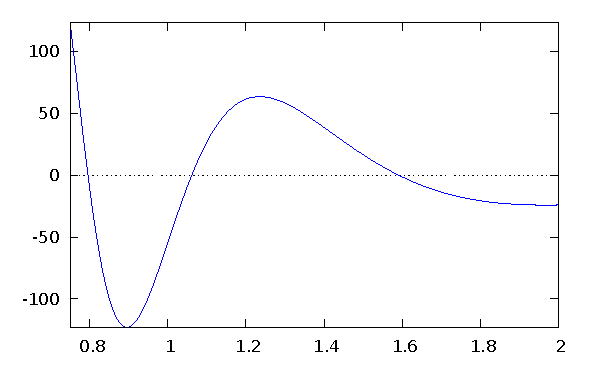
\includegraphics[width=5.5cm]{figures/roots-bisection3}
\par\end{center}
\item Misalkan Anda hendak mencari akar dari $f(x)=x-e^{-x}$ dengan metode
bagi dua. Tentukan sebuah bilangan bulat $a$ sedemikian sehingga
interval $[a,a+2]$ merupakan interval yang sesuai untuk memulai pencarian.
\item Tentukan batas bawah bagi jumlah iterasi yang diperlukan untuk menjamin
akurasi $10^{-20}$ pada soal \ref{enu:useBisection}.
\item \label{exc:bisection-3}Berapa langkah (iterasi) metode bagi dua yang
diperlukan untuk menjamin solusi dengan akurasi $10^{-10}$ jika suatu
akar diketahui berada di dalam $[4.5,5.3]$? \hasananswer 
\item Misalkan Anda menggunakan metode bagi dua pada interval yang panjangnya
3. Berapa iterasi yang diperlukan untuk menjamin bahwa hampiran akurat
hingga $10^{-6}$?
\item Misalkan suatu fungsi $g$ memenuhi asumsi-asumsi metode bagi dua
pada interval yang diberikan. Berawal dari interval tersebut, berapa
iterasi yang diperlukan untuk menghampiri akar dengan toleransi yang
diberikan?

\begin{enumerate}
\item $[-7,10]$; $10^{-6}$
\item $[5,9]$; $10^{-3}$
\item $[9,15]$; $10^{-10}$
\item $[-6,-1]$; $10^{-105}$ (anggaplah komputer menghitung dengan 300
angka signifikan sehingga galat pembulatan tidak menjadi masalah)
\end{enumerate}
\item \octave\ $1$ merupakan akar dari $f(x)=\ln(x^{4}\text{\textminus}x^{3}\text{\textminus}7x^{2}+13x\text{\textminus}5)$
yang tidak dapat dijamin akan ditemukan oleh metode bagi dua. 

\begin{enumerate}
\item Gunakan grafik fungsi di sekitar $1$ untuk menjelaskan mengapa demikian.
Anda dapat menggunakan kode Octave di bawah ini untuk membuat grafik
yang sesuai.
\item Meskipun demikian, jalankan metode bagi dua pada $f$ untuk interval
$[0.8,1.2]$. Apa yang terjadi alih-alih metode tersebut menemukan
akar?
\end{enumerate}
\begin{verbatim}
x=0.8:.01:1.2;
f=@(x) log(x.^4-x.^3-7*x.^2+13*x-5);
plot(x,f(x)) 
\end{verbatim}
\item \octave\ $4$ merupakan akar dari $g(x)=|\sin(\pi x)|$  yang tidak
dapat ditemukan dengan metode bagi dua. 

\begin{enumerate}
\item Gunakan grafik fungsi di sekitar $4$ untuk menjelaskan mengapa demikian.
Anda dapat menggunakan kode Octave di bawah ini untuk membuat grafik
yang sesuai.
\item Meskipun demikian, jalankan metode bagi dua pada $g$ untuk interval
$[3.5,4.5]$. Apa yang terjadi alih-alih metode tersebut menemukan
akar?
\end{enumerate}
\begin{verbatim}
x=3.5:.05:4.5;
f=@(x) abs(sin(pi*x));
plot(x,f(x)) 
\end{verbatim}
\item \label{exc:bisection-4}Misalkan $f(x)=\sin(x^{2})$. $f$ kontinu
pada $[4,5]$, tetapi $f(4)<0$ dan $f(5)<0$, sehingga asumsi-asumsi
metode bagi dua tidak terpenuhi. Meskipun demikian, metode bagi dua
sebagaimana dijelaskan dalam kode semu, jika diterapkan pada $f$
di interval $[4,5]$ \textit{tetap} menghasilkan sebuah akar. Jelaskan. \hasasolution 
\item Fungsi-fungsi pada soal \ref{enu:failure1}, \ref{enu:failure2},
dan \ref{enu:failure3} semuanya tidak memenuhi asumsi-asumsi metode
bagi dua pada interval $[-4,-0.5]$. Untuk setiap fungsi, jelaskan
bagaimana asumsi tersebut gagal terpenuhi.
\item \label{exc:bisection-5}\octave\ Tulislah sebuah fungsi Octave bernama
\texttt{collatz} yang menerima satu masukan bilangan bulat, $n$,
dan mengembalikan $3n+1$ jika $n$ ganjil, serta $n/2$ jika $n$
genap. Simpan fungsi tersebut sebagai berkas \texttt{collatz.m}. Gunakan
pernyataan \texttt{if then else} dalam fungsi Anda. PETUNJUK: Gunakan
fungsi pembulatan ke atas dari Octave. Jika \texttt{ceil(n/2)} sama
dengan \texttt{n/2}, maka \texttt{n} pasti genap (tidak bersisa jika
dibagi 2). Gunakan fungsi \texttt{collatz} Anda untuk menghitung \hasananswer 

\begin{enumerate}
\item \texttt{collatz(17)}
\item \texttt{collatz(10)}
\item \texttt{collatz(109)}
\item \texttt{collatz(344)}
\end{enumerate}
\item \octave\ Tulislah fungsi nilai mutlak Anda sendiri yang bernama \texttt{absval}
(\texttt{abs} sudah didefinisikan oleh Octave, sehingga sebaiknya
Anda menggunakan nama lain), yang menerima masukan bilangan riil dan
mengembalikan nilai mutlak masukan tersebut. Gunakan pernyataan \texttt{if
then else} dalam fungsi Anda. Simpan fungsi tersebut sebagai \texttt{absval.m}
dan ujilah dengan perhitungan berikut. 

\begin{enumerate}
\item $|-3|$
\item $|123.2|$
\item $\left|\pi-\frac{22}{7}\right|$
\item $|10-\pi^{2}|$
\end{enumerate}
\item \label{exc:bisection-6}$f(x)=\sin(x^{2})$ memiliki lima akar pada
interval $[7,8]$. $f(7)<0$, $f(8)>0$, dan $f$ kontinu pada $[7,8]$,
sehingga asumsi-asumsi metode bagi dua terpenuhi. Metode tersebut
akan konvergen ke suatu akar.

\begin{enumerate}
\item Gunakan berkas \texttt{bisection.m} Anda (Latihan \ref{exc:bisectionCode})
untuk menentukan akar mana yang diperoleh. \hasananswer 
\item Temukan 4 interval berbeda yang membuat metode bagi dua konvergen
ke empat akar lainnya di $[7,8]$.
\end{enumerate}
\item Fungsi yang ditampilkan memiliki akar kira-kira di $2.41$, $4.11$,
$5.62$, $7.01$, $8.32$, $9.57$, $10.78$, dan $11.94$. Dengan
interval awal yang diberikan, ke akar mana metode bagi dua akan konvergen?

\begin{center}
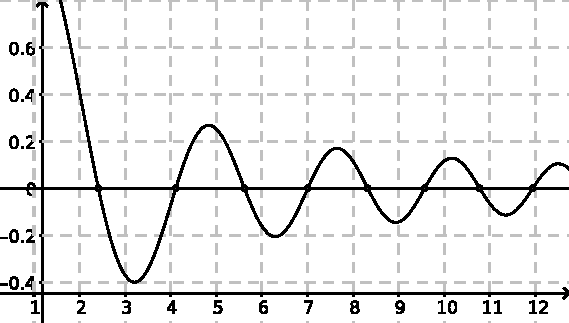
\includegraphics[scale=0.6]{figures/roots-bisection2}
\par\end{center}
\begin{enumerate}
\item $[2,3]$
\item $[6,8]$
\item $[2,6]$
\item $[5,9]$
\item $[10,12]$ Catatan: asumsi metode bagi dua tidak terpenuhi pada interval
ini. Meskipun demikian, metode sebagaimana diuraikan dalam kode semu
\textit{akan} konvergen ke suatu akar!
\end{enumerate}
\item Carilah interval dengan panjang 1 yang memungkinkan metode bagi dua
diterapkan untuk mencari akar dari $f(x)=x^{4}-7.6746x^{3}-40.7477022x^{2}+200.9894434x+319.0914281$.
\item Algoritma berikut merupakan salah satu bentuk metode bagi dua.

\begin{pseudocode} 
\begin{description}
\item [{Asumsi:}] $f$ kontinu pada $[a,b]$. $f(a)$ dan $f(b)$ memiliki
tanda yang berlawanan.
\item [{Masukan:}] Interval $[a,b]$; fungsi $f$
\item [{Langkah~1:}] Untuk $j=1\ldots15$ lakukan Langkah 2 dan 3:

\begin{description}
\item [{Langkah~2:}] Tetapkan $m=\frac{a+b}{2}$;
\item [{Langkah~3:}] Jika $f(a)f(m)<0$ maka tetapkan $b=m$; jika tidak,
tetapkan $a=m$;
\end{description}
\item [{Langkah~4:}] Cetak $m$.
\item [{Keluaran:}] Hampiran $m$.
\end{description}
\end{pseudocode} 
\begin{enumerate}
\item Terapkan algoritma ini pada fungsi $f(x)=(x)(x-2)(x+2)$ pada interval
$[-3,3]$. Akar manakah yang akan dihampiri algoritma ini?
\item Berapakah batas galat yang dijamin bagi hampiran tersebut menurut
rumus
\[
|p_{n}-p|\leq\frac{b-a}{2^{n}}?
\]
\item Seberapa akurat hampiran tersebut sebenarnya? Bandingkan dengan batas
pada (b).
\item Ubahlah algoritma agar dapat menghampiri akar yang berbeda dengan
menggunakan interval awal yang sama.
\item Ubahlah algoritma agar tidak menggunakan perkalian.
\end{enumerate}
\item \label{bisectionCode-1}Gunakan kode semu berikut untuk menulis implementasi
metode bagi dua yang sedikit berbeda. Lihat Tabel \ref{tab:commonOctave}
jika Anda belum yakin cara memprogram besaran $\lceil(\ln(b-a)-\ln(TOL))/\ln2\rceil$.
Perulangan while dibahas pada \vpageref{subsec:WhileLoop}.

\begin{description}
\item [{Masukan:}] fungsi $f$, titik ujung $a$ dan $b$; toleransi $TOL$.
\item [{Kembalikan}] solusi hampiran $p$ beserta nilai $f(p)$ dan jumlah
iterasi yang telah dilakukan $N_{0}$.
\item [{Langkah~1}] Tetapkan $i=1$; $FA=f(a)$; $N_{0}=\lceil(\ln|b-a|-\ln(TOL))/\ln2\rceil$;
\item [{Langkah~2}] Selama $i\leq N_{0}$ lakukan Langkah 3 sampai 6.

\begin{description}
\item [{Langkah~3}] Tetapkan $p=(a+b)/2$; $FP=f(p)$;
\item [{Langkah~4}] Jika $FP=0$ maka\\
$\qquad$Kembalikan($p$, $f(p)$, $i$); BERHENTI.
\item [{Langkah~5}] Tetapkan $i=i+1$;
\item [{Langkah~6}] Jika $FA\cdot FP>0$ maka\\
$\qquad$Tetapkan $a=p$; $FA=FP$;\\
jika tidak\\
$\qquad$Tetapkan $b=p$;
\end{description}
\item [{Langkah~7}] Kembalikan($p$, $f(p)$, $N_{0}$);\\
BERHENTI.
\end{description}
\begin{enumerate}
\item Bahas kelebihan dan kekurangan algoritma ini dibandingkan dengan algoritma
pada \vpageref{bisectionCode}.
\item Dari manakah perhitungan $N_{0}=\lceil(\ln(b-a)-\ln(TOL))/\ln2\rceil$
diperoleh?
\end{enumerate}
\item Gunakan kode yang Anda tulis untuk soal \ref{bisectionCode-1} untuk
mencari solusi dengan galat tidak lebih dari $10^{-5}$ bagi persoalan-persoalan
berikut. 

\begin{enumerate}
\item $x-2^{x}+.95=0$ pada $[0,1]$
\item $e^{x}-x^{2}+3x-2=0$ pada $[0,1]$
\item $2x\cos(2x)-(x+1)^{2}=0$ pada $[-3,-2]$ dan pada $[-1,0]$
\end{enumerate}
\item Carilah hampiran $\sqrt{3}$ dengan galat tidak lebih dari $10^{-4}$
menggunakan metode bagi dua. Tulislah esai tentang cara Anda menyelesaikan
masalah ini. Sertakan kode metode bagi dua Anda, fungsi dan interval
yang Anda gunakan, serta alasan pemilihannya.
\item Sebuah palung sepanjang $L$ memiliki penampang berbentuk setengah
lingkaran berjari-jari $r$. Jika diisi air hingga permukaan air berada
pada jarak $h$ dari bagian atas, volume air $V$ adalah 
\[
V=L\left[0.5\pi r^{2}-r^{2}\arcsin\left(\frac{h}{r}\right)-h\sqrt{r^{2}-h^{2}}\right]
\]
Misalkan $L=10$ kaki, $r=1$ kaki, dan $V=12.4$ kaki$^{3}$. Tentukan
kedalaman air di dalam palung dengan galat tidak lebih dari 0,01 kaki.
Catatan: Di Octave, gunakan \texttt{asin(x)} untuk $\arcsin(x)$ dan
\texttt{pi} untuk $\pi$.
\end{enumerate}
\finishexercises

\subsection*{Jawaban}
\begin{description}
\item [{Berapakah~nilai~yang~diperoleh~berikutnya?}] \label{subsec:bisectionAnswer1}
$T_{2}(3.25)-\ln(3.25)\approx.10429$, yang melebihi nilai sasaran.
Jadi $3.25$ menjadi titik ujung kiri yang baru, dan nilai berikutnya
adalah $\frac{3.25+3.5}{2}=3.375$, yaitu titik tengah dari $3.25$
dan $3.5$.
\item [{Titik~ujung~kanan~adalah~$13.13$:}] \label{subsec:bisectionAnswer2}
Dengan memulai dari $a=10$ dan $b=14$, perhatikan bahwa $g(a)\approx.088>0$
dan $g(b)\approx-.044<0$, sehingga nilai $g$ pada titik ujung kiri
harus selalu positif dan nilai $g$ pada titik ujung kanan harus selalu
negatif:
\end{description}
\begin{center}
\begin{tabular}{ccccc}
$a$ & $m$ & $b$ & $g(m)$ & \tabularnewline
\hline 
10 & 12 & 14 & $.044$ & $\Rightarrow m$ menjadi titik ujung kiri\tabularnewline
12 & 13 & 14 & $.006$ & $\Rightarrow m$ menjadi titik ujung kiri\tabularnewline
13 & $13.5$ & 14 & $-.017$ & $\Rightarrow m$ menjadi titik ujung kanan\tabularnewline
13 & $13.25$ & $13.5$ & $-.005$ & $\Rightarrow m$ menjadi titik ujung kanan\tabularnewline
13 & $13.125$ & $13.25$ & $.0004$ & $\Rightarrow m$ menjadi titik ujung kiri\tabularnewline
$13.125$ & $13.1875$ & $13.25$ & $-.002$ & $\Rightarrow m$ menjadi titik ujung kanan\tabularnewline
$13.125$ & $13.15625$ & $13.1875$ & $-.0009$ & $\Rightarrow m$ menjadi titik ujung kanan\tabularnewline
$13.125$ & $13.140625$ & $13.15625$ & $-.0002$ & $\Rightarrow m$ menjadi titik ujung kanan\tabularnewline
$13.125$ & $13.1328125$ & $13.140625$ &  & \tabularnewline
\end{tabular}
\par\end{center}



\section{\label{sec:Fixedpt}Iterasi Titik Tetap\index{metode iterasi titik tetap}
\index{metode!iterasi titik tetap|see{metode iterasi titik tetap}}}

Ambil kalkulator Anda. Kalkulator apa pun yang memiliki tombol kosinus
sudah memadai. Jika Anda menggunakan kalkulator ilmiah sederhana,
tekan tombol hapus semua, yang biasanya bertanda \texttt{AC} atau
cukup \texttt{C}. Layar kini seharusnya menampilkan 0. Tekan tombol
kosinus, yang seharusnya bertanda \texttt{cos}. Layar seharusnya menampilkan
1. Tekan lagi tombol kosinus. Layar seharusnya menampilkan $0.540302\ldots$.
Ulangi. Ulangi lagi. Bahkan, teruslah menekan tombol kosinus sampai
Anda melihat suatu pola. 

Jika Anda memiliki kalkulator yang lebih canggih dengan tombol jawaban
sebelumnya, biasanya bertanda \texttt{Ans}, tekan 0 lalu \texttt{Enter}
atau \texttt{=}. Kemudian tekan tombol kosinus lalu tombol jawaban
sebelumnya. Setelah itu, tekan \texttt{Enter} atau \texttt{=} untuk
melakukan perhitungan. Pada kali pertama, layar seharusnya menampilkan
1 (sama seperti pada kalkulator ilmiah). Namun, untuk mengulanginya,
cukup tekan \texttt{Enter} atau \texttt{=} lagi. Tindakan ini akan
mengulangi perhitungan terakhir, yaitu kosinus dari jawaban sebelumnya.
Layar seharusnya menampilkan $0.540302\ldots$. Sekarang ulangi sampai
Anda melihat suatu pola.

Setelah sekitar 30 pengulangan, atau yang akan kita sebut iterasi\index{iterasi},
kalkulator Anda seharusnya menampilkan bilangan seperti $0.739083847\ldots$.
Berapa kali pun Anda mengulangi, atau mengiterasi, perhitungan itu,
nilainya tidak akan banyak berubah. Bahkan, setelah mencapai $0.7390851332\ldots$,
nilainya tidak akan berubah sama sekali (kecuali kalkulator Anda menampilkan
lebih banyak tempat desimal---setelah sekitar 90 iterasi, kalkulator
yang menampilkan 15 tempat desimal akan menunjukkan $0.739085133215161$
dan nilainya tidak akan berubah lagi). Artinya, $\cos(0.7390851332\ldots)=0.7390851332\ldots$.
Kita menyebut $0.7390851332\ldots$ sebagai \index{titik tetap} titik
tetap dari fungsi kosinus. Nilai itu tetap (tidak berubah) ketika
fungsi kosinus diterapkan. Dengan kata lain, pada $0.7390851332\ldots$,
masukan dan keluaran fungsi kosinus sama. Lihat simulasi iterasi ini
secara daring di \href{http://lqbrin.github.io/tea-time-numerical/ancillaries.html}{situs pendamping}.

Barangkali sekarang muncul serangkaian pertanyaan. Mengapa ini berhasil?
Bagaimana jika kita mulai dengan bilangan selain 0? Apakah ini berhasil
untuk sembarang fungsi? Dapatkah kita meramalkan kapan cara ini akan
berhasil atau tidak? Dapatkah kita mencari akar dengan cara ini? Apakah
kekonvergenannya cepat? Dalam bagian ini dan bagian berikutnya, kita
akan memberikan setidaknya jawaban parsial untuk semua pertanyaan
tersebut. Kita mulai dengan ``Mengapa ini berhasil?''.

Perhatikan penyelesaian sistem 
\[
\begin{cases}
y=\cos(x)\\
y=x
\end{cases}.
\]
Salah satu cara menyelesaikannya adalah dengan metode substitusi.
Jika kita menyubstitusikan $y=x$ ke dalam $y=\cos x$ kita memperoleh
$x=\cos x$ atau $\cos x=x$. Solusi sistem tersebut tepat berimpit
dengan titik-titik tetap fungsi kosinus, karena setiap solusi $\cos x=x$
merupakan nilai $x$ yang tidak berubah oleh fungsi kosinus. Karena
sistem dua persamaan dengan dua peubah dapat diselesaikan, setidaknya
secara hampiran, dengan menggambar grafik, hal ini menyarankan agar
kita melihat grafik sistem tersebut untuk memahami lebih jauh apa
yang terjadi selama iterasi.

\begin{figure}[h]
\caption{\label{fig:cosine-fixed-point}Menentukan titik tetap $\cos(x)$.}

\bigskip{}

\centering{}%
\begin{tabular}{cccc}
(a) &  & (b) & \tabularnewline
 & 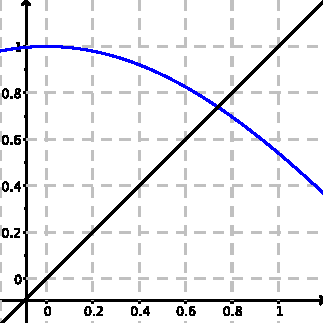
\includegraphics{figures/roots-fixedpt5} &  & 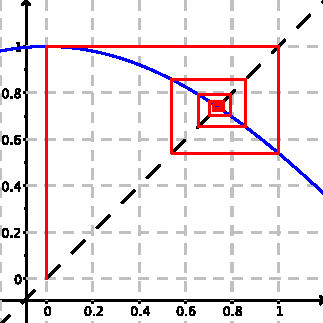
\includegraphics{figures/roots-fixedpt1}\tabularnewline
\end{tabular}
\end{figure}
Gambar \ref{fig:cosine-fixed-point}(a) memperlihatkan grafik $y=\cos(x)$
dan $y=x$ pada interval $[0,1]$. Kita dapat melihat titik potong
di sekitar $(0.75,0.75)$ sehingga kita patut menduga bahwa titik
tetapnya berada di sekitar $0.75$ (yang tentu saja kita ketahui benar
dari percobaan kalkulator). Gambar \ref{fig:cosine-fixed-point}(b)
menggambarkan proses menghitung $\cos(0),\cos(1),\cos(0.540302\ldots),\ldots$.
Menelusuri ruas garis vertikal dari $(0,0)$ ke $(0,1)$ menunjukkan
perhitungan $\cos(0)$. Menelusuri kelanjutan horizontal dari $(0,1)$
ke $(1,1)$ lalu ruas garis vertikal dari $(1,1)$ ke $(1,0.540302\ldots)$
menunjukkan perhitungan $\cos(1)$. Menelusuri garis horizontal dari
$(1,0.540302\ldots)$ ke $(0.540302\ldots,0.540302\ldots)$ lalu garis
vertikal dari $(0.540302\ldots,0.540302\ldots)$ ke $(0.540302\ldots,0.857553\ldots)$
menunjukkan perhitungan $\cos(0.540302\ldots)$, dan seterusnya. Setiap
pasangan ruas garis---yang satu bergerak horizontal dari grafik $y=\cos(x)$
menuju grafik $y=x$ dan yang lain bergerak vertikal dari garis $y=x$
menuju grafik $y=\cos(x)$---menunjukkan satu iterasi lagi. Gambar
\ref{fig:cosine-fixed-point}(b) kadang disebut diagram jaring\index{diagram jaring}
\cite{barnsley}, dan lazim digunakan untuk menggambarkan konsep iterasi.
Lintasan diagram jaring yang menuju $(0.739085\ldots,0.739085\ldots)$
merupakan akibat tak terhindarkan dari geometri grafik $\cos(x)$.

Bagaimana jika kita mulai dengan bilangan selain 0? Dengan menggunakan
Gambar \ref{fig:cosine-fixed-point}, Anda seharusnya dapat meyakinkan
diri bahwa kekonvergenan menuju titik $(0.7390851332\ldots,0.7390851332\ldots)$
terjamin untuk setiap nilai awal antara 0 dan 1. Cobalah. Mulailah
dari sembarang titik pada garis $y=x$. Bergeraklah secara vertikal
ke grafik $y=\cos(x)$. Lalu bergeraklah secara horizontal ke garis
$y=x$. Ulangi. Anda akan mendapati bahwa lintasan diagram jaring
selalu menuju perpotongan kedua grafik. Sekarang pertimbangkan untuk
memulai dengan sembarang bilangan real, $r$. Kosinus setiap bilangan
real berada dalam interval $[-1,1]$ sehingga $\cos(r)\in[-1,1]$.
Kosinus setiap bilangan dalam interval $[-1,1]$ berada dalam interval
$[0,1]$ sehingga $\cos(\cos(r))\in[0,1]$. Artinya, iterasi kedua
berada dalam interval dari 0 sampai 1. Jadi, hanya setelah dua iterasi,
setiap nilai awal akan menjadi nilai antara 0 dan 1. Diagram jaring
kita menunjukkan bahwa iterasi selanjutnya akan menuju titik tetap.
Jadi, apa pun nilai awalnya, iterasi menuju titik tetap. Argumen sebelumnya
menjadi cikal bakal bukti fakta ini.

Namun, tidak semua fungsi berperilaku sebaik itu. Sebagai contoh,
$1^{2}=1$. Dengan kata lain, $1$ adalah titik tetap fungsi $y=x^{2}$.
Akan tetapi, iterasi yang dimulai dari sembarang bilangan selain $1$
atau $-1$ tidak menuju titik tetap ini. Jika kita mulai dengan sembarang
bilangan yang lebih besar dari 1 lalu menguadratkannya, nilainya menjadi
lebih besar. Jika hasilnya dikuadratkan, nilainya menjadi lebih besar
lagi. Menguadratkannya sekali lagi hanya memperbesar nilai tersebut
tanpa batas. Oleh karena itu, iterasi yang dimulai dari sembarang
nilai yang lebih besar dari 1 (atau lebih kecil dari $-1$) tidak
konvergen ke titik tetap $1$. Demikian pula iterasi yang dimulai
dari sembarang bilangan yang nilai mutlaknya kurang dari 1. Gambar
\ref{fig:quadratic-fixed-point} 
\begin{figure}[h]
\caption{\label{fig:quadratic-fixed-point}Memvisualisasikan iterasi $f(x)=x^{2}$.}

\bigskip{}

\centering{}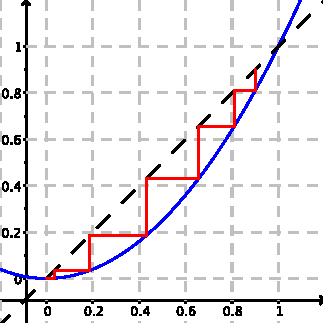
\includegraphics[scale=1.2]{figures/roots-fixedpt2}
\end{figure}
 menggambarkan iterasi $y=x^{2}$ dengan nilai awal $0.9$. Ikuti
diagram jaring dari titik $(0.9,0.9)$ secara vertikal ke grafik $y=x^{2}$
lalu secara horizontal kembali ke garis $y=x$, dan seterusnya, untuk
memeriksanya sendiri. Ini menggambarkan dengan baik fakta bahwa kuadrat
setiap bilangan yang terletak ketat antara 0 dan 1 lebih kecil daripada
bilangan itu sendiri. Untuk nilai awal antara $-1$ dan $1$, dengan
mengecualikan $\pm1$, iterasi menghasilkan barisan yang konvergen
ke 0, bukan 1. Singkatnya, selain $-1$ dan 1, tidak ada nilai awal
yang menghasilkan barisan yang konvergen ke 1 di bawah iterasi fungsi
$y=x^{2}$.

Terdapat perbedaan mendasar antara titik tetap $0.7390851332\ldots$
dari $f(x)=\cos(x)$ dan titik tetap $1$ dari $g(x)=x^{2}$. Iterasi
titik tetap konvergen ke $0.7390851332\ldots$ di bawah $f(x)=\cos(x)$
untuk sembarang nilai awal. Iterasi titik tetap gagal konvergen ke
$1$ di bawah $g(x)=x^{2}$ untuk semua nilai awal kecuali $\pm1$.\footnote{Untuk jenis perilaku ketiga, iterasi titik tetap konvergen ke $0$
di bawah $g(x)$ untuk nilai awal di dekat 0, tetapi tidak untuk nilai
awal lainnya!} Memeriksa grafik $f(x)$ dan $g(x)$ yang masing-masing ditumpangtindihkan
dengan garis $y=x$ di lingkungan titik tetapnya dapat memberi petunjuk
{[}Gambar \ref{fig:fixed-pt-zoom}{]} tentang perbedaannya. 
\begin{figure}[h]
\caption{\label{fig:fixed-pt-zoom}Kiri: \textcolor{blue}{$f(x)=\cos(x)$}
dan $y=x$. Kanan: \textcolor{blue}{$g(x)=x^{2}$} dan $y=x$. }

\bigskip{}

\centering{}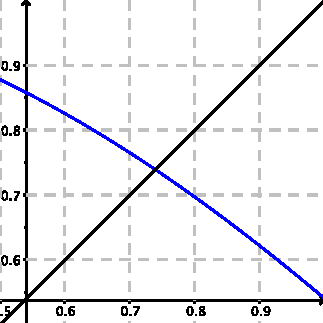
\includegraphics{figures/roots-fixedpt3} 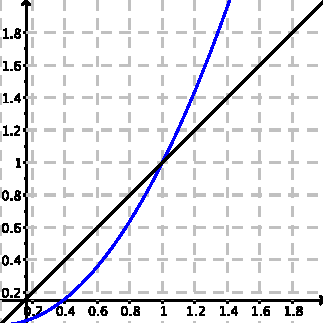
\includegraphics{figures/roots-fixedpt4}
\end{figure}
Memang, $f(x)$ memiliki gradien negatif di titik tetapnya, sedangkan
$g(x)$ memiliki gradien positif di titik tetapnya. Anda dapat melihatnya
dari grafik atau ``melakukan kalkulusnya''. Namun, perbedaan yang
penting lebih halus. Bukan tanda gradien di titik tetap yang menentukan.
Nilai mutlak gradien di titik tetaplah yang menentukan. Untuk fungsi
mulus, lingkungan titik-titik dengan nilai mutlak gradien lebih besar
dari 1 cenderung ekspansif. Artinya, titik-titik saling menjauh ketika
fungsi diterapkan. Sebaliknya, lingkungan titik-titik dengan nilai
mutlak gradien kurang dari 1 cenderung kontraktif. Artinya, titik-titik
saling mendekat ketika fungsi diterapkan. 
\begin{prop}
\label{prop:contractive}Jika $h(x)$ dapat didiferensialkan pada
$(a,b)$ dengan $|h'(x)|<1$ untuk semua $x\in(a,b)$, maka untuk
setiap $x_{1},x_{2}\in(a,b)$, $|h(x_{2})-h(x_{1})|<|x_{2}-x_{1}|$.
\end{prop}

\begin{proof}
Ambil $x_{1},x_{2}\in(a,b)$ dan, tanpa mengurangi keumuman, ambil
$x_{2}>x_{1}$ agar kita dapat dengan tepat merujuk pada interval
dari $x_{1}$hingga $x_{2}$. Karena $h(x)$ kontinu pada $[x_{1},x_{2}]$
dan dapat didiferensialkan pada $(x_{1},x_{2})$, Teorema Nilai Rata-Rata
memberi kita $c\in(x_{1},x_{2})\subseteq(a,b)$ sedemikian sehingga
$h'(c)=\left|\frac{h(x_{2})-h(x_{1})}{x_{2}-x_{1}}\right|$. Namun,
$h'(c)<1$ menurut asumsi, sehingga $h'(c)=\left|\frac{h(x_{2})-h(x_{1})}{x_{2}-x_{1}}\right|<1$,
yang langsung memberikan $|h(x_{2})-h(x_{1})|<|x_{2}-x_{1}|$.
\end{proof}
Selain itu, fungsi yang nilai mutlak turunannya kurang dari 1 hanya
dapat memotong garis $y=x$ satu kali. Setelah memotongnya, fungsi
tersebut tidak pernah dapat ``menyusul'' karena hal itu membutuhkan
gradien yang lebih besar dari 1, yaitu gradien garis $y=x$. 
\begin{prop}
\label{prop:uniquenessOfFixedPoint}Misalkan $h(x)$ kontinu pada
$[a,b]$, dapat didiferensialkan pada $(a,b)$ dengan $|h'(x)|<1$
untuk semua $x\in(a,b)$, dan $h([a,b])\subseteq[a,b]$. Maka $h$
mempunyai tepat satu titik tetap dalam $[a,b]$.
\end{prop}

\begin{proof}
Jika $h(a)=a$ atau $h(b)=b$, keberadaan telah terbukti. Karena itu,
misalkan $h(a)\neq a$ dan $h(b)\neq b$. Karena $h([a,b])\subseteq[a,b]$
harus berlaku $h(a)>a$ dan $h(b)<b$. Langsung diperoleh $h(a)-a>0$
dan $h(b)-b<0$. Karena fungsi bantu $f(x)=h(x)-x$ kontinu pada $[a,b]$,
Teorema Nilai Antara menjamin adanya $c\in(a,b)$ sedemikian sehingga
$f(c)=0$. Dengan substitusi, $h(c)-c=0$, yang menyiratkan $h(c)=c$,
sehingga $c$ adalah titik tetap $h$. Keberadaan titik tetap telah
terbukti. Sekarang misalkan $c_{1}\in[a,b]$ dan $c_{2}\in[a,b]$
adalah titik-titik tetap yang berbeda dari $h$. Maka 
\[
\frac{h(c_{1})-h(c_{2})}{c_{1}-c_{2}}=\frac{c_{1}-c_{2}}{c_{1}-c_{2}}=1.
\]
 Berdasarkan Teorema Nilai Rata-Rata, terdapat $c_{3}$ di antara
$c_{1}$ dan $c_{2}$ sedemikian sehingga $h'(c_{3})=1$, yang bertentangan
dengan fakta bahwa $|h'(x)|<1$ untuk semua $x\in(a,b)$. Oleh karena
itu, tidak mungkin $c_{1}$ dan $c_{2}$ berbeda.
\end{proof}
Jadi, kita dapat secara wajar menduga bahwa jika nilai mutlak turunan
di suatu titik tetap kurang dari 1, iterasi merupakan metode yang
layak untuk menghampiri (menentukan) titik tetap tersebut, sedangkan
jika nilai mutlak turunan di suatu titik tetap lebih besar dari 1,
iterasi bukan metode yang layak untuk menghampiri titik tetap itu.
Namun, kita harus berhati-hati agar tidak menganggap kaidah praktis
ini mutlak. Kaidah ini hanya berlaku untuk apa yang disebut fungsi
yang berperilaku baik. Dalam hal ini, memiliki turunan pertama yang
kontinu di lingkungan titik tetap sudah cukup untuk disebut berperilaku
baik. Teorema berikut menetapkan bahwa iterasi titik tetap akan konvergen
dalam suatu lingkungan titik tetap jika nilai mutlak turunan fungsi
kurangdari 1 di sana. 
\begin{thm}
\label{thm:fixedPointConvergence}(Teorema Kekonvergenan Titik Tetap)
\index{Teorema!Kekonvergenan Titik Tetap} Diberikan suatu fungsi
$f(x)$ dengan turunan pertama yang kontinu dan titik tetap $\hat{x}$,
jika $|f'(\hat{x})|<1$ maka terdapat suatu lingkungan $\hat{x}$
tempat iterasi titik tetap konvergen ke titik tetap tersebut untuk
setiap nilai awal dalam lingkungan itu.
\end{thm}

\begin{proof}
Dari kekontinuan, terdapat $\varepsilon>0$ sedemikian sehingga $|f'(x)|<1$
untuk semua $x\in(\hat{x}-\varepsilon,\hat{x}+\varepsilon)$. Ambil
$0<\delta<\varepsilon$ dan tetapkan ${\displaystyle M=\max_{x\in[\hat{x}-\delta,\hat{x}+\delta]}|f'(x)|}$.
Sekarang misalkan $x_{0}$ adalah suatu nilai tertentu tetapi sembarang
dalam $(\hat{x}-\delta,\hat{x}+\delta)$. Seperti pada Proposisi \ref{prop:contractive},
kita menerapkan Teorema Nilai Rata-Rata. Kali ini, dijamin terdapat
${\displaystyle c\in(\hat{x}-\delta,\hat{x}+\delta)}$ sedemikian
sehingga $f'(c)=\frac{f(\hat{x})-f(x_{0})}{\hat{x}-x_{0}}$. Namun,
$|f'(c)|\leq M$ sehingga $|f(\hat{x})-f(x_{0})|\leq M|\hat{x}-x_{0}|$.
Selain itu, $\hat{x}$ adalah titik tetap, sehingga $f(\hat{x})=\hat{x}$,
dan dari sini diperoleh $|\hat{x}-f(x_{0})|\leq M|\hat{x}-x_{0}|$.
Sekarang kita mendefinisikan $x_{k}=f(x_{k-1})$ untuk semua $k\geq1$
dan membuktikan dengan induksi bahwa $|\hat{x}-x_{k}|\leq M^{k}|\hat{x}-x_{0}|$
untuk semua $k\geq1$. Karena $x_{1}=f(x_{0})$, kita telah menunjukkan
$|\hat{x}-x_{1}|\leq M|\hat{x}-x_{0}|$, sehingga klaim benar ketika
$k=1$. Sekarang misalkan $|\hat{x}-x_{k}|\leq M^{k}|\hat{x}-x_{0}|$
untuk suatu nilai tertentu tetapi sembarang $k\geq1$. Perhatikan
bahwa $|\hat{x}-x_{k}|\leq M^{k}|\hat{x}-x_{0}|$ menyiratkan $x_{k}\in(\hat{x}-\delta,\hat{x}+\delta)$
sehingga kita menerapkan Teorema Nilai Rata-Rata seperti sebelumnya
dan menyimpulkan $|\hat{x}-f(x_{k})|\leq M|\hat{x}-x_{k}|$. Dengan
mengganti $x_{k+1}$ dengan $f(x_{k})$ dan menggunakan hipotesis
induksi, kita memperoleh $|\hat{x}-x_{k+1}|\leq M\cdot M^{k}|\hat{x}-x_{0}|=M^{k+1}|\hat{x}-x_{0}|$.
Jadi, kita mempunyai $0\leq|\hat{x}-x_{k}|\leq M^{k}|\hat{x}-x_{0}|$.
Tentu saja ${\displaystyle \lim_{k\to\infty}0=0}$ dan ${\displaystyle \lim_{k\to\infty}M^{k}|\hat{x}-x_{0}|=0}$,
sehingga berdasarkan Teorema Apit, ${\displaystyle \lim_{k\to\infty}|\hat{x}-x_{k}|=0}$.
\end{proof}
Seperti disinggung sebelumnya, kita tidak semestinya mengharapkan
iterasi titik tetap konvergen ketika nilai mutlak turunan di suatu
titik tetap lebih besar dari satu. Bahkan, yang terjadi kurang lebih
adalah kebalikannya. Terdapat suatu lingkungan titik tetap yang pasti
ditinggalkan oleh iterasi titik tetap untuk setiap nilai awal di lingkungan
itu selain titik tetaptersebut. Mengingat fakta itu, kita tergoda
untuk berpikir bahwa Teorema Kekonvergenan TitikTetap mungkin dapat
diperkuat menjadi implikasi dua arah, yaitu pernyataan jika dan hanyajika.
Dan hal itu ``hampir'' dapat dilakukan. Pernyataan yang dapat dibuat
di sini memiliki padanan langsung dengan uji rasio untuk deret. Ingatlah
bahwa untuk setiap barisan bilangan real $a_{0},a_{1},a_{2},\ldots$,
limit ${\displaystyle L=\lim_{k\to\infty}\left|\frac{a_{k+1}}{a_{k}}\right|}$
membantu menentukan kekonvergenan ${\displaystyle \sum_{k=0}^{\infty}a_{k}}$
sebagai berikut:
\begin{itemize}
\item Jika $L<1$, maka ${\displaystyle \sum_{k=0}^{\infty}a_{k}}$ konvergen
(mutlak).
\item Jika $L>1$, maka ${\displaystyle \sum_{k=0}^{\infty}a_{k}}$ divergen.
\item Jika $L=1$, maka ${\displaystyle \sum_{k=0}^{\infty}a_{k}}$ dapat
konvergen (mutlak atau bersyarat), atau dapat divergen.
\end{itemize}
Secara analog, untuk setiap fungsi $f(x)$ dengan turunan pertama
yang kontinu dan titik tetap $\hat{x}$, turunan $f'(\hat{x})$ membantu
menentukan kekonvergenan metode iterasi titik tetap sebagai berikut:
\begin{itemize}
\item Jika $|f'(\hat{x})|<1$, maka iterasi titik tetap konvergen ke $\hat{x}$
untuk setiap nilai awal dalam suatu lingkungan $\hat{x}$.
\item Jika $|f'(\hat{x})|>1$, maka terdapat suatu lingkungan $\hat{x}$
yang ditinggalkan oleh iterasi titik tetap untuk setiap nilai awal
di lingkungan tersebut selain $\hat{x}$.
\item Jika $|f'(\hat{x})|=1$, maka iterasi titik tetap dapat konvergen
ke $\hat{x}$ untuk setiap nilai awal dalam suatu lingkungan $\hat{x}$;
atau dapat meninggalkan suatu lingkungan untuk setiap nilai awal di
lingkungan tersebut selain $\hat{x}$; atau mungkin tidak ada lingkungan
yang membuat semua nilai awal menghasilkan kekonvergenan dan juga
tidak ada lingkungan yang membuat semua nilai selain $\hat{x}$ meninggalkannya.
\end{itemize}
Grafik fungsi-fungsi yang turunannya sama dengan satu di titik tetap
masing-masing pada Gambar \ref{fig:derivativeEqualsOne} membantu
menggambarkan kasus terakhir ini.

\begin{center}
\begin{figure}
\caption{\label{fig:derivativeEqualsOne}Perilaku kekonvergenan ketika turunan
di titik tetap sama dengan 1.}

\bigskip{}

\centering{}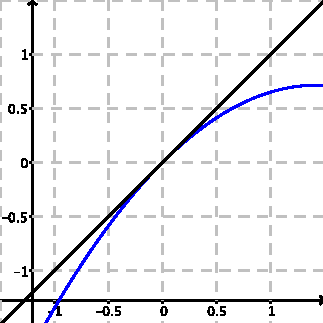
\includegraphics[scale=0.8]{figures/roots-fixedpt6} 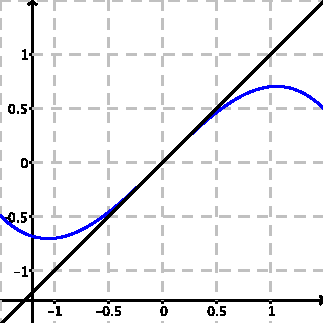
\includegraphics[scale=0.8]{figures/roots-fixedpt7}
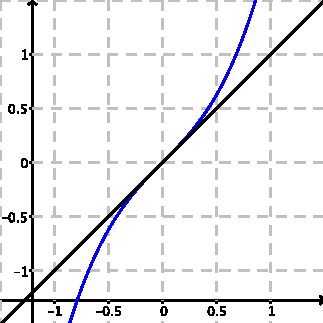
\includegraphics[scale=0.8]{figures/roots-fixedpt8}
\end{figure}
\par\end{center}

\noindent Pada salah satu fungsi ini, iterasi titik tetap konvergen
untuk semua nilai dalam suatu lingkungan titik tetap. Pada fungsi
lainnya, iterasi titik tetap meninggalkan suatu lingkungan titik tetap
untuk semua nilai awal di lingkungan tersebut kecuali titik tetap
itu sendiri. Pada fungsi ketiga, iterasi titik tetap konvergen ke
titik tetap untuk beberapa nilai awal dan meninggalkan suatu lingkungan
titik tetap untuk nilai awal lainnya (dan \textit{setiap} lingkungan
titik tetap akan memuat kedua jenis nilai awal). Dapatkah Anda menentukan
yang mana? Temukan jawabannya dengan membuat diagram jaring untuk
masing-masing. Jawaban \vpageref{subsec:Answers-fixedPointIteration}.

Bukti Teorema Kekonvergenan Titik Tetap dapat dengan mudah diperluas
untuk mencakup nilai awal dalam sembarang lingkungan titik tetap tempat
nilai mutlak turunan tetap kurang dari $1$. Ukuran dan kesimetrian
interval tidak penting. Sebagai contoh, $f(x)=\frac{1}{8}x^{3}-x^{2}+2x+1$
memiliki titik tetap di $\hat{x}=2$. Bukti Teorema Kekonvergenan
Titik Tetap menetapkan kekonvergenan menuju $2$ dalam interval simetris
di sekitar $2$ misalnya $[1.9,2.1]$. Namun, interval ini jauh dari
lingkungan terbesar nilai-nilai awal yang membuat iterasi titik tetap
konvergen ke $2$. Kita dapat mencari batas-batas interval terbesar
semacam itu dengan menyelesaikan persamaan $|f'(x)|=1$. Untuk itu:
\begin{eqnarray*}
\frac{3}{8}x^{2}-2x+2 & = & \pm1\\
3x^{2}-16x+16 & = & \pm8\\
3x^{2}-16x+24=0 & atau & 3x^{2}-16x+8=0\\
x=\frac{8\pm i2\sqrt{2}}{3} & atau & x=\frac{8\pm2\sqrt{10}}{3}\\
\frac{8-2\sqrt{10}}{3}\approx0.558 & dan & \frac{8+2\sqrt{10}}{3}\approx4.775,
\end{eqnarray*}
Jadi, kita patut mengharapkan iterasi titik tetap konvergen ke 2 pada
setiap interval tertutup yang termuat dalam
\[
\left(\frac{8-2\sqrt{10}}{3},\frac{8+2\sqrt{10}}{3}\right).
\]
 Sekarang, jika kita meminta komputer menjalankan iterasi titik tetap
untuk sejumlah besar nilai awal yang berjarak sama, misalnya 100 nilai,
pada interval $[-2,8]$ lalu mencatat hasilnya pada garis bilangan
dengan mewarnai suatu nilai awal hitam jika tidak konvergen ke 2 dan
hijau jika konvergen ke 2 (diagram semacam itu akan kita sebut diagram
kekonvergenan), kita memperoleh

\begin{center}
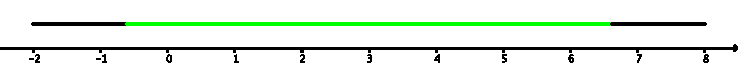
\includegraphics{figures/roots-fixedpt9},
\par\end{center}

\noindent yang menunjukkan bahwa iterasi titik tetap konvergen ke
2 untuk nilai awal pada interval kira-kira $[-0.5,6.5]$. Memang,
eksperimen tersebut menegaskan bahwa iterasi titik tetap konvergen
pada setiap interval tertutup yang termuat dalam $\left(\frac{8-2\sqrt{10}}{3},\frac{8+2\sqrt{10}}{3}\right)$
sebagaimana diprediksi. Namun, diagram itu menunjukkan kekonvergenan
pada himpunan yang bahkan lebih besar. Kita dapat menyimpulkan bahwa
Teorema Kekonvergenan Titik Tetap memberikan syarat yang cukup, tetapi
bukan syarat yang perlu, bagi kekonvergenan dalam suatu lingkungan
titik tetap. 

Grafik fungsi $f(x)$ yang ditumpangtindihkan dengan garis $y=x$
(Gambar \ref{fig:basinOfAttractionExplanation}) 
\begin{figure}
\caption{\label{fig:basinOfAttractionExplanation}$f(x)=\frac{1}{8}x^{3}-x^{2}+2x+1$
dan garis $y=x$}

\centering{}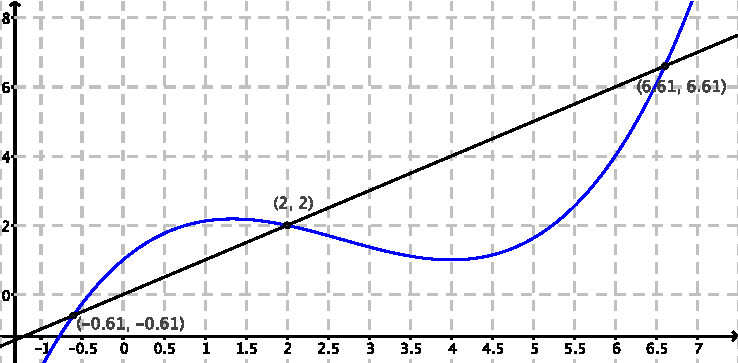
\includegraphics{figures/roots-fixedpt10}
\end{figure}
 memberi gambaran mengapa batas $\frac{8\pm2\sqrt{10}}{3}$ belum
menceritakan keseluruhan keadaan. Dengan membayangkan diagram jaring
untuk sembarang nilai awal di antara dua titik tetap selain 2, yakni
$-0.61$ dan $6.61$, Anda seharusnya dapat meyakinkan diri bahwa
iterasi titik tetap konvergen ke $2$ untuk sembarang nilai awal dalam
interval $(-0.61,6.61)$. Dapatkah Anda membuktikannya? Grafik seperti
dalam Gambar \ref{fig:fixed-pt-zoom}, \ref{fig:derivativeEqualsOne},
dan \ref{fig:basinOfAttractionExplanation} sangat diperlukan dan
harus selalu diperiksa ketika mencoba memahami iterasi titik tetap,
tetapi grafik tersebut tidak boleh dijadikan bukti. Untuk pembuktian,
kita perlu mengandalkan teorema seperti Teorema Kekonvergenan Titik
Tetap.

\noindent\begin{digression}{Sebuah kuadrat yang menarik} 

\noindent Mencoba mencari akar persamaan logistik 
\[
g(x)=(\alpha-1)x-\alpha x^{2}
\]
dengan menerapkan iterasi titik tetap pada fungsi yang bersesuaian
$f(x)=x+g(x)=\alpha x(1-x)$ merupakan latihan terkenal dalam sistem
dinamis, tetapi cara ini terkenal sering tidak berhasil! Selesaikan
penyelidikan berikut untuk melihat apa yang terjadi.
\begin{enumerate}
\item Tunjukkan bahwa $f(x)=\alpha x(1-x)$ seperti yang dinyatakan.
\item Untuk setiap nilai $\alpha=2.5$, $\alpha=3.2$, $\alpha=3.833$,
dan $\alpha=4$, lakukan langkah-langkah berikut.

\begin{enumerate}
\item Tentukan secara analitis titik tetap positif dari $f$ (akar $g$)
(dengan pensil, kertas, dan sedikit aljabar). 
\item Tetapkan $x_{0}=0.1$ dan gunakan program komputer untuk menghitung
$x_{975}$ sampai $x_{1000}$.
\item Amati 26 hasil iterasi pada bagian (b) dan jelaskan apa yang Anda
lihat.
\end{enumerate}
\item Hubungkan hasil yang Anda peroleh pada bagian 2 dengan diagram berikut.

\begin{center}
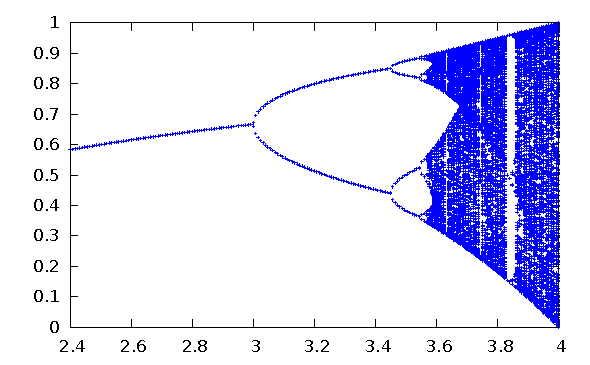
\includegraphics{figures/phaseDiagram}
\par\end{center}
\item Gunakan diagram tersebut untuk memperkirakan nilai $\alpha$ yang
menurut Anda akan membuat iterasi titik tetap menghasilkan $x_{975}$
sampai $x_{1000}$ yang berulang dalam siklus empat nilai berbeda.
Periksa perkiraan Anda.
\end{enumerate}
\noindent\end{digression}

\subsection{Pencarian Akar\label{subsec:RootFindingInvestigation}}

Jika berhasil, iterasi titik tetap menemukan solusi persamaan berbentuk
$f(x)=x$. Masalah pencarian akar menuntut solusi persamaan berbentuk
$g(x)=0$. Namun, persamaan $f(x)=x$ memiliki solusi yang persis
sama dengan persamaan $f(x)-x=0$, sehingga mencari titik tetap $f(x)$
ekuivalen dengan mencari akar $g(x)=f(x)-x$. Memang, contoh pencarian
titik tetap $f(x)=\frac{1}{8}x^{3}-x^{2}+2x+1$ dapat kita nyatakan
ulang sebagai masalah pencarian akar $g(x)=f(x)-x=\frac{1}{8}x^{3}-x^{2}+x+1$.
Akan tetapi, justru masalah sebaliknya jauh lebih umum. Kita dihadapkan
pada masalah mencari akar suatu fungsi dan perlu menyatakannya ulang
sebagai masalah titik tetap.

Misalkan kita ingin mencari akar $g(x)=-x^{3}+5x^{2}-4x-6$. Pertanyaan
untuk menyelesaikan $g(x)=0$ dapat kita nyatakan ulang sebagai masalah
mencari titik tetap dari banyak fungsi yang berbeda! Namun, untuk
menurunkan fungsi-fungsi itu, Anda harus mengabaikan beberapa nasihat
bijak guru aljabar Anda! Kuncinya adalah menggunakan aljabar untuk
menulis ulang persamaan $-x^{3}+5x^{2}-4x-6=0$ sebagai persamaan
berbentuk $x=f(x)$. Cara paling sederhana adalah menambahkan $x$
pada kedua ruas persamaan. Manipulasi ini dan beberapa manipulasi
lainnya ditunjukkan dalam daftar berikut.
\begin{itemize}
\item $-x^{3}+5x^{2}-4x-6=0\Rightarrow-x^{3}+5x^{2}-3x-6=x$
\item $-x^{3}+5x^{2}-4x-6=0\Rightarrow-x^{3}+5x^{2}-6=4x\Rightarrow\frac{-x^{3}+5x^{2}-6}{4}=x$
\item $-x^{3}+5x^{2}-4x-6=0\Rightarrow-x^{3}-4x-6=-5x^{2}\Rightarrow\frac{x^{3}+4x+6}{5}=x^{2}\Rightarrow\pm\sqrt{\frac{x^{3}+4x+6}{5}}=x$
\item $-x^{3}+5x^{2}-4x-6=0\Rightarrow5x^{2}-4x-6=x^{3}\Rightarrow\sqrt[3]{5x^{2}-4x-6}=x$
\end{itemize}
Dapatkah Anda melihat apa yang dilakukan pada masing-masing baris?
Dengan demikian, kita memiliki lima kandidat untuk iterasi titik tetap,
$f_{1}(x)=-x^{3}+5x^{2}-3x-6$, $f_{2}(x)=\frac{-x^{3}+5x^{2}-6}{4}$,
$f_{3}(x)=\sqrt{\frac{x^{3}+4x+6}{5}}$, $f_{4}(x)=-\sqrt{\frac{x^{3}+4x+6}{5}}$,
dan $f_{5}(x)=\sqrt[3]{5x^{2}-4x-6}$, yang semuanya berpotensi menghasilkan
akar $g(x)$. Ada fungsi keenam yang akan kita bahas jauh lebih rinci
nanti: $f_{6}(x)=\frac{2x^{3}\text{\textminus}5x^{2}\text{\textminus}6}{3x^{2}\text{\textminus}10x+4}$\footnote{Dengan menghitung $f_{6}(1-\sqrt{3})$, $f_{6}(1+\sqrt{3})$, dan
$f_{6}(3)$, Anda dapat memverifikasi bahwa $f_{6}$ juga memiliki
ketiga nilai ini sebagai titik tetap.}. 
\begin{figure}
\caption{\label{fig:SixConvergenceDiagrams}Diagram kekonvergenan bagi 6 fungsi
dengan titik tetap yang sama.}

\bigskip{}

\begin{centering}
$f_{1}$: 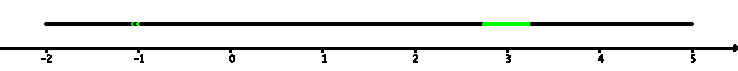
\includegraphics{figures/roots-fixedpt11}
\par\end{centering}
\begin{centering}
$f_{2}$: 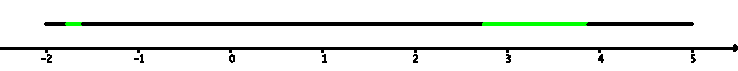
\includegraphics{figures/roots-fixedpt12}
\par\end{centering}
\begin{centering}
$f_{3}$: 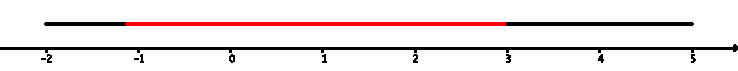
\includegraphics{figures/roots-fixedpt13}
\par\end{centering}
\begin{centering}
$f_{4}$: 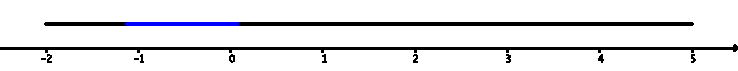
\includegraphics{figures/roots-fixedpt14}
\par\end{centering}
\begin{centering}
$f_{5}$: 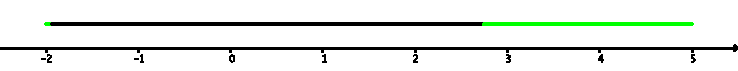
\includegraphics{figures/roots-fixedpt15}
\par\end{centering}
\begin{centering}
$f_{6}$: 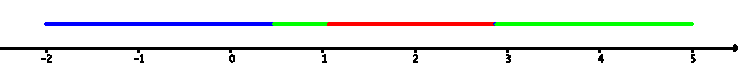
\includegraphics{figures/roots-fixedpt16}
\par\end{centering}
\centering{}hitam: tidak konvergen; hijau: konvergen ke $3$; merah:
konvergen ke $1+\sqrt{3}$; biru: konvergen ke $1-\sqrt{3}$
\end{figure}
 Akar-akar $g(x)$ adalah $1-\sqrt{3}\approx-0.73$, $1+\sqrt{3}\approx2.73$,
dan $3$, sehingga kita akan meninjau diagram kekonvergenan pada interval
$[-2,5]$. Iterasi titik tetap konvergen ke titik tetap yang berbeda
untuk fungsi yang berbeda meskipun keenam fungsi memiliki tepat tiga
titik tetap yang sama. Diagram kekonvergenan pada Gambar \ref{fig:SixConvergenceDiagrams}
diberi kode warna untuk menggambarkan kenyataan ini. Seperti sebelumnya,
warna hitam menunjukkan ketakkonvergenan. Warna hijau, merah, dan
biru masing-masing menunjukkan kekonvergenan ke $3$, $1+\sqrt{3}$,
dan $1-\sqrt{3}$, secara berurutan. Perhatikan bahwa hanya $f_{6}$
yang menghasilkan kekonvergenan, sejauh yang dapat kita ketahui, untuk
setiap nilai awal dalam $[-2,5]$, dan fungsi ini juga merupakan satu-satunya
fungsi yang membuat iterasi titik tetap konvergen ke titik tetap berbeda
untuk nilai awal berbeda. Cobalah memahami alasan perilaku kekonvergenan
setiap fungsi dengan mengamati grafik $f_{1},f_{2},\ldots,f_{6}$.
Berikan perhatian khusus pada grafik di sekitar $1+\sqrt{3}$ dan
$3$. Tampilan grafik dapat menyesatkan di daerah itu karena kedua
titik tetap sangat berdekatan. Coba juga temukan dua nilai awal dalam
$[-2,5]$ yang menyebabkan iterasi titik tetap dengan $f_{6}$ tidak
konvergen. Lalu, apa yang terjadi? Sebagai tantangan tambahan, cobalah
menemukan nilai ketiga dalam $[-2,5]$ yang menyebabkan iterasi titik
tetap dengan $f_{6}$ tidak konvergen. Petunjuk: Anda mungkin perlu
menggunakan sistem aljabar komputer untuk menemukan nilai semacam
itu secara eksak, atau menggunakan iterasi titik tetap untuk menghampirinya!
Jawaban \vpageref{subsec:Answers-fixedPointIteration}.

\subsection{Metode Iterasi Titik Tetap (kode semu)\index{metode iterasi titik tetap!kode semu}}

Meskipun kita telah banyak membahas cara menentukan apakah metode
iterasi titik tetap diperkirakan akan konvergen atau tidak, tak satu
pun informasi tersebut diperlukan secara langsung untuk mengodekan
metode itu. Setiap implementasi metode ini harus memungkinkan pengguna
mencoba iterasi titik tetap untuk sembarang fungsi dengan sembarang
nilai awal. Pengguna bertanggung jawab memahami bahwa ketika asumsi-asumsinya
tidak terpenuhi, hasilnya tidak dapat diprediksi. Ingat, ``sampah
masuk...sampah keluar.''

Metode iterasi titik tetap menimbulkan masalah yang tidak terdapat
pada metode bagi dua. Dalam metode bagi dua, terdapat rumus yang sederhana
dan praktis untuk batas atas galat. Untuk menyediakan hal serupa dalam
metode iterasi titik tetap, kita harus mengorbankan kesederhanaan,
kepraktisan, atau keduanya, sedangkan manfaatnya tidak sebanding dengan
pengorbanan tersebut. Sebagai gantinya, digunakan kriteria penghentian
yang lebih umum. Ketika dua nilai iterasi berturut-turut lebih dekat
satu sama lain daripada toleransi yang diberikan, metode berhenti.
Pada saat itu, selisih antara nilai iterasi, katakanlah $x_{k}$ dan
$x_{k+1}$, lebih kecil daripada toleransi. Untuk barisan yang dihasilkan
oleh iterasi titik tetap, $x_{k+1}=f(x_{k})$, sehingga $|x_{k+1}-x_{k}|=|f(x_{k})-x_{k}|$.
Ketika $|x_{k+1}-x_{k}|$ kecil, $|f(x_{k})-x_{k}|$ juga kecil, sehingga
$f(x_{k})\approx x_{k}$. $x_{k}$ ``hampir'' merupakan titik tetap.

\begin{pseudocode} 
\begin{description}
\item [{Asumsi:}] $f$ terdiferensialkan. $f$ mempunyai titik tetap $\hat{x}$.
$x_{0}$ berada dalam lingkungan $(\hat{x}-\delta,\hat{x}+\delta)$
tempat nilai mutlak $f'$ kurang dari satu.
\item [{Masukan:}] Nilai awal $x_{0}$; fungsi $f$; akurasi yang diinginkan
$tol$; jumlah maksimum iterasi $N$.
\item [{Langkah~1:}] Untuk $j=1\ldots N$ lakukan Langkah 2-4:

\begin{description}
\item [{Langkah~2:}] Tetapkan $x=f(x_{0})$;
\item [{Langkah~3:}] Jika $|x-x_{0}|\leq tol$ maka kembalikan $x$;
\item [{Langkah~4:}] Tetapkan $x_{0}=x$;
\end{description}
\item [{Langkah~5:}] Cetak ``Metode gagal. Jumlah maksimum iterasi terlampaui.''
\item [{Keluaran:}] Hampiran $x$ yang mendekati titik tetap eksak, atau
pesan kegagalan.
\end{description}
\end{pseudocode}  

\subsection{Konsep Utama}
\begin{description}
\item [{Titik~tetap:}] $x_{0}$ adalah titik tetap fungsi $f(x)$ jika
$f(x_{0})=x_{0}$.
\item [{Iterasi~titik~tetap:}] \index{metode iterasi titik tetap} Menghitung
barisan $x_{0},x_{1}=f(x_{0}),x_{2}=f(x_{1}),x_{3}=f(x_{2}),\ldots$
berdasarkan fungsi $f$ dan nilai awal $x_{0}$.
\item [{Titik~tetap~atraktif:}] Suatu titik tetap disebut \index{titik tetap!atraktif}
atraktif (atau penarik) jika terdapat lingkungan titik tetap tersebut
yang membuat iterasi titik tetap konvergen untuk semua nilai awal
di dalam lingkungan itu.
\item [{Titik~tetap~repulsif:}] Suatu titik tetap disebut \index{titik tetap!repulsif}
repulsif (atau penolak) jika iterasi titik tetap meninggalkan suatu
lingkungan titik tetap tersebut untuk sembarang nilai awal di dalam
lingkungan itu selain titik tetap itu sendiri.
\item [{Teorema~Nilai~Rata-Rata:}] \index{Teorema!Nilai Rata-Rata}Jika
$f$ kontinu pada $[a,b]$ dan dapat didiferensialkan pada $(a,b)$,
maka terdapat $c\in(a,b)$ sedemikian sehingga $f'(c)=\frac{f(b)-f(a)}{b-a}$.
\item [{Teorema~Kekonvergenan~Titik~Tetap:}] \index{Teorema!Kekonvergenan Titik Tetap}
Diberikan suatu fungsi $f(x)$ dengan turunan pertama yang kontinu
dan titik tetap $\hat{x}$, jika $|f'(\hat{x})|<1$ maka terdapat
suatu lingkungan $\hat{x}$ tempat iterasi titik tetap konvergen ke
titik tetap tersebut untuk setiap nilai awal dalam lingkungan itu.
\end{description}
\startexercises

\subsection{Latihan}
\begin{enumerate}
\item \label{enu:fixedPtIterationCode}Tulislah fungsi Octave yang mengimplementasikan
metode iterasi titik tetap. Simpan fungsi tersebut sebagai berkas
\texttt{.m} untuk digunakan di kemudian hari.
\item \label{enu:mvtExamples}(i) Tentukan apakah fungsi pada interval tersebut
memenuhi hipotesis Teorema Nilai Rata-Rata. (ii) Jika hipotesis terpenuhi,
carilah nilai $c$ yang keberadaannya dijamin oleh teorema tersebut.

\begin{enumerate}
\item $f(x)=3-x-\sin x$; $[2,3]$
\item $g(x)=3x^{4}-2x^{3}-3x+2$; $[0,1]$
\item \label{exc:fixedpt}$g(x)=3x^{4}-2x^{3}-3x+2$; $[0,0.9]$ \hasasolution 
\item \label{exc:fixedpt-16}$h(x)=10-\cosh(x)$; $[-3,-2]$ \hasananswer 
\item $f(t)=\sqrt{4+5\sin t}-2.5$; $[-6,-5]$
\item \label{exc:fixedpt-1}$g(t)=\frac{3t^{2}\tan t}{1-t^{2}}$; $[20,23]$ \hasasolution 
\item \label{exc:fixedpt-2}$h(t)=\ln(3\sin t)-\frac{3t}{5}$; $[2,4]$ \hasananswer 
\item \label{exc:fixedpt-3}$f(r)=e^{\sin r}-r$; $[-20,20]$ \hasananswer 
\item $g(r)=\sin(e^{r})+r$; $[-3,3]$
\item $h(r)=2^{\sin r}-3^{\cos r}$; $[1,3]$
\end{enumerate}
\item Carilah semua titik tetap fungsi tersebut secara eksak. Gunakan aljabar.

\begin{enumerate}
\item $f(x)=\sqrt[3]{2x^{3}-x^{2}-x}$
\item $f(x)=\frac{\ln(2e^{x})}{2}$
\item \label{exc:fixedpt-4}$f(x)=\log(x^{2}-3x)-1+x$ \hasananswer 
\item \label{exc:fixedpt-5}$g(x)=3x^{2}+5x+1$ \hasananswer 
\item $g(t)=t+\frac{5000}{1+2e^{-3t}}-2500$
\item $g(x)=e^{\ln(x+1)-3}$
\item $h(x)=\sqrt{4x^{2}+4x+1}$
\item \label{exc:fixedpt-6}$h(x)=x-10+3^{x}+25\cdot3^{-x}$ \hasasolution 
\item $h(x)=x+6-3\log_{5}(2x)$
\end{enumerate}
\item Carilah setidaknya dua fungsi kandidat, $f_{1}(x)$ dan $f_{2}(x)$,
untuk mencari akar $g(x)$ melalui iterasi titik tetap. Dengan kata
lain, ubah masalah mencari akar $g$ menjadi masalah mencari titik
tetap $f_{1}$ atau $f_{2}$.

\begin{enumerate}
\item $g(x)=7x^{2}+5x-9$
\item $g(x)=x+\cos x$
\item \label{exc:fixedpt-7}$g(x)=6x^{5}+12x^{2}-8$ \hasananswer 
\item \label{exc:fixedpt-8}$g(x)=x^{2}-e^{3x+4}$ \hasasolution 
\item $g(x)=7x-3\cos(\pi x-2)+\ln|2x^{2}+4x-8|$
\item \label{exc:fixedpt-9}$g(x)=3^{x^{2}-5x+1}-2^{-x^{2}-5x-1}$ \hasananswer 
\end{enumerate}
\item \label{enu:fixedPtIterationExamples}Hitung 5 iterasi pertama metode
iterasi titik tetap dengan menggunakan fungsi dan nilai awal yang
diberikan. Berdasarkan kelima iterasi ini, apakah Anda memperkirakan
metode tersebut akan konvergen?

\begin{enumerate}
\item $f(x)=3-\sin x$; $x_{0}=2$
\item \label{exc:fixedpt-10}$g(x)=10+x-\cosh(x)$; $x_{0}=-3$ \hasasolution 
\item \label{exc:fixedpt-11}$h(t)=\ln(3\sin t)+\frac{2t}{5}$; $t_{0}=1$ \hasananswer 
\item $w(r)=2^{\sin r}-3^{\cos r}+r$; $r_{0}=1$
\end{enumerate}
\item \label{enu:usingOctave}Gunakan fungsi Octave Anda dari soal \ref{enu:fixedPtIterationCode}
untuk setiap pasangan fungsi dan nilai awal pada soal \ref{enu:fixedPtIterationExamples}.
Atur toleransi menjadi $10^{-10}$ dan jumlah maksimum iterasi menjadi
100. Untuk setiap pasangan, apakah metode tersebut konvergen dalam
paling banyak 100 iterasi? Jika ya, ke nilai berapa? Laporkan setidaknya
10 angka signifikan. \haspartwithsolution  \haspartwithanswer 
\item \label{enu:usingWeb}Buatlah diagram jaring untuk setiap pasangan
fungsi/nilai awal pada soal \ref{enu:fixedPtIterationExamples}. \haspartwithsolution  \haspartwithanswer 
\item Bandingkan hasil dari soal \ref{enu:usingOctave} dengan hasil dari
soal \ref{enu:usingWeb}. Apakah keduanya konsisten?
\item Gunakan Proposisi \ref{prop:uniquenessOfFixedPoint} untuk menunjukkan
bahwa $g(x)=2x(1-x)$ mempunyai tepat satu titik tetap pada $[0.3,0.7]$.
\item \label{exc:fixedpt-12}Misalkan $f(x)=\frac{3x^{2}\text{\textminus}1}{6x+4}$. \hasasolution 

\begin{enumerate}
\item Tunjukkan bahwa $f$ mempunyai tepat satu titik tetap pada $[-4,-0.9]$.
\item Gunakan iterasi titik tetap untuk mencari hampiran titik tetap dengan
galat tidak lebih dari $10^{-2}$.
\end{enumerate}
\item \label{enu:ShowPart2}Misalkan $g(x)=\pi+0.5\sin(x/2)$.

\begin{enumerate}
\item Tunjukkan bahwa $g$ mempunyai tepat satu titik tetap pada $[0,2\pi]$. 
\item Gunakan iterasi titik tetap untuk mencari hampiran titik tetap dengan
galat tidak lebih dari $10^{-2}$.
\end{enumerate}
\item \label{exc:fixedpt-13}Tunjukkan bahwa metode iterasi titik tetap
yang diterapkan pada $f(x)=\sqrt[3]{8-4x}$ akan konvergen ke suatu
akar $g(x)=x^{3}+4x-8$ untuk setiap nilai awal $x_{0}\in[1.2,1.5]$. \hasasolution 
\item Tunjukkan bahwa iterasi titik tetap dijamin konvergen ke titik tetap
dari
\[
f(x)=(\sqrt{2})^{x}
\]
untuk setiap $x_{0}\in[1,3]$. PETUNJUK: $f'(x)=\frac{1}{2}\ln(2)\cdot(\sqrt{2})^{x}$.
\item Misalkan $g(x)=x^{2}-3x-2$. 

\begin{enumerate}
\item Carilah fungsi $f$ yang membuat iterasi titik tetap konvergen ke
suatu akar $g$. 
\item Gunakan fungsi tersebut untuk mencari akar $g$ dengan galat tidak
lebih dari $10^{-3}$ dari nilai eksaknya.
\item Nyatakan nilai awal yang Anda gunakan dan banyaknya iterasi yang diperlukan
untuk memperoleh hampiran tersebut.
\end{enumerate}
\item Gunakan iterasi titik tetap dengan $p_{0}=-1$ untuk menghampiri akar
$g(x)=x^{3}-3x+3$ hingga ketelitian $10^{-4}$.
\item Gunakan suatu metode iterasi titik tetap untuk mencari hampiran $\sqrt{3}$
dengan galat tidak lebih dari $10^{-4}$. Fungsi Anda hanya boleh
menggunakan konstanta bilangan bulat. Fungsi dan nilai awal apa yang
Anda gunakan?
\item Fungsi $g(x)=x^{4}+2x^{2}-x-3$ mempunyai dua akar. Salah satunya
berada dalam $[-1,0]$ dan yang lainnya berada dalam $[1,2]$.

\begin{enumerate}
\item Sebagai persiapan untuk mencari akar $g(x)$ dengan iterasi titik
tetap, salah satu cara memanipulasi persamaan $x^{4}+2x^{2}-x-3=0$
adalah dengan menambahkan $x$ pada kedua ruas. Hasilnya
\[
x=x^{4}+2x^{2}-3
\]
Buatlah grafik yang sesuai untuk menentukan apakah iterasi fungsi
$f(x)=x^{4}+2x^{2}-3$ akan menemukan akar dalam $[-1,0]$. Bagaimana
dengan akar dalam $[1,2]$? Jelaskan bagaimana Anda memperoleh kesimpulan
tersebut.
\item \label{root1}Manipulasilah persamaan $x^{4}+2x^{2}-x-3=0$ sedemikian
rupa sehingga iterasi titik tetap berhasil menemukan akar dalam $[-1,0]$.
Gambarlah grafik yang menunjukkan bahwa metode Anda akan berhasil.
\item \label{root2}Apakah manipulasi yang sama memungkinkan Anda menemukan
akar dalam $[1,2]$? Jika tidak, carilah manipulasi lain yang dapat
melakukannya. Sekali lagi, tampilkan grafik yang menunjukkan bahwa
metode Anda akan berhasil.
\item Gunakan metode Anda dari bagian \ref{root1} dan \ref{root2} untuk
mencari kedua akar hingga 3 tempat desimal.
\end{enumerate}
\item \label{exc:fixedpt-14}Iterasi titik tetap pada $f(x)=\sqrt[3]{2x^{3}-x^{2}-x}$
tidak akan konvergen ke suatu titik tetap. Akan tetapi, iterasi titik
tetap pada fungsi $g(x)=\sqrt[3]{x^{2}+x}$ akan konvergen kira-kira
ke $1.618033988749895$ untuk setiap $x_{0}$ dalam $[0.5,3.5]$. \hasananswer 

\begin{enumerate}
\item Berapa banyak iterasi yang diperlukan untuk mencapai akurasi $10^{-4}$
dengan menggunakan $g(x)$ dengan $x_{0}=2.5$?
\item Jelaskan mengapa $f(x)$ dan $g(x)$ mempunyai titik-titik tetap yang
sama.
\end{enumerate}
\item Carilah satu nol (nol mana pun) dari $g(x)=x^{2}+10\cos x$ dengan
galat tidak lebih dari $10^{-4}$ menggunakan iterasi titik tetap.
Nyatakan:

\begin{enumerate}
\item fungsi $f$ yang Anda gunakan dalam iterasi titik tetap
\item nilai awal, $x_{0}$, yang Anda gunakan
\item jumlah iterasi yang diperlukan
\end{enumerate}
\item \label{enu:fixedExp}Misalkan $c$ adalah bilangan real tak nol. Tunjukkan
bahwa setiap titik tetap tak nol dari $f(x)=xe^{c\cdot g(x)}$ merupakan
akar dari $g$.
\item Hampiri $\sqrt{3}$ dengan metode yang disarankan oleh soal \ref{enu:fixedExp}.
\item \label{enu:findC}Misalkan $g(\hat{x})=0$, $g$ memiliki turunan
pertama yang kontinu, dan $g'(\hat{x})\neq0$. Tunjukkan bahwa terdapat
suatu nilai $c$ sehingga iterasi titik tetap pada $f(x)=x+cg(x)$
konvergen ke $\hat{x}$ dalam suatu lingkungan $\hat{x}$.
\item \label{exc:fixedpt-15}Tentukan nilai $c$ yang menjamin bahwa iterasi
titik tetap untuk fungsi $f(x)=x+c(x-5\cos x)$ konvergen dari sembarang
nilai awal $x_{0}\in[0,\pi/2]$. Jelaskan. \hasananswer 
\item Misalkan $g(x)=$$\frac{1}{2}^{x}+\frac{1}{5}^{x}-10^{-5}$. 

\begin{enumerate}
\item Tunjukkan bahwa jika $g(x)$ memiliki nol di $p$, maka fungsi $f(x)=x+cg(x)$
memiliki titik tetap di $p$.
\item \label{findc}Tentukan nilai $c$ sehingga iterasi titik tetap pada
$f(x)$ konvergen untuk setiap nilai awal, $p_{0}$, dalam interval
$[16,17]$. Buat sketsa grafik yang menunjukkan bahwa pilihan $c$
Anda tepat.
\item Gunakan fungsi dari bagian \ref{findc} dengan nilai $c$ yang telah
Anda tentukan untuk mencari akar $g(x)$ yang akurat hingga $10^{-4}$.
Nyatakan nilai yang Anda gunakan untuk $p_{0}$. Tunjukkan tiga iterasi
terakhir. Berapa iterasi yang diperlukan?
\end{enumerate}
\item Buktikan bahwa untuk $f(x)=\cos x$, iterasi titik tetap konvergen
untuk setiap nilai awal.
\item \label{enu:convergenceStrengthened}Teorema Kekonvergenan Titik Tetap
dapat diperkuat. Syarat bahwa turunan pertama harus kontinu dapat
diganti. Ubah bukti dalam teks untuk menunjukkan pernyataan berikut.

\textit{Diberikan suatu fungsi $f(x)$ yang dapat didiferensialkan
dengan titik tetap $\hat{x}$, jika $|f'(x)|\leq M<1$ untuk setiap
$x$ dalam suatu lingkungan $\hat{x}$, maka iterasi titik tetap konvergen
ke titik tetap tersebut untuk setiap nilai awal dalam lingkungan itu.}
\item Buat tiga grafik yang serupa dengan grafik pada Gambar \ref{fig:derivativeEqualsOne}
untuk menganalisis keadaan ketika turunan di titik tetap sama dengan
$-1$. Apakah keadaan itu berbeda dari keadaan ketika turunan di titik
tetap sama dengan $1$?
\end{enumerate}
\noindent\finishexercises

\subsection*{Jawaban\label{subsec:Answers-fixedPointIteration}}
\begin{description}
\item [{Gambar~\ref{fig:derivativeEqualsOne}:}] Dari kiri ke kanan: setiap
lingkungan titik tetap memuat kedua jenis nilai awal; iterasi titik
tetap konvergen untuk semua nilai dalam suatu lingkungan titik tetap;
iterasi titik tetap meninggalkan suatu lingkungan titik tetap untuk
semua nilai awal dalam lingkungan itu kecuali titik tetap itu sendiri.
\item [{Gambar~\ref{fig:SixConvergenceDiagrams}:}] Ketika penyebutnya
nol, $f_{6}(x)$ tidak terdefinisi (terdapat asimtot vertikal pada
grafik), sehingga kita menyelesaikan $3x^{2}\text{\textminus}10x+4=0$
untuk memperoleh dua nilai awal yang menyebabkan iterasi titik tetap
gagal (karena iterasi pertama tidak terdefinisi). Nilai-nilai itu
adalah $x=\frac{5\pm\sqrt{13}}{3}\approx.4648\mbox{ dan }2.868$.
Untuk mencari titik ketiga yang menyebabkan iterasi titik tetap gagal,
kita menyelesaikan persamaan $f_{6}(x)=\frac{5+\sqrt{13}}{5}$ (kita
juga dapat menyelesaikan $f_{6}(x)=\frac{5-\sqrt{13}}{5}$ sebagai
gantinya). Maka iterasi kedua tidak terdefinisi karena iterasi pertama
menghasilkan $\frac{5+\sqrt{13}}{5}$. Satu-satunya solusi real kira-kira
$1.055909763230534$, yang dapat ditemukan melalui iterasi titik tetap
pada $\sqrt[3]{\frac{\sqrt{13}x^{2}+10x^{2}\text{\textminus}\frac{10\sqrt{13}x}{3}\text{\textminus}\frac{50x}{3}+\frac{4\sqrt{13}}{3}+\frac{38}{3}}{2}}$.
Buktikan. Namun, perhatikan bahwa pernyataan bahwa iterasi titik tetap
akan gagal didasarkan pada asumsi aritmetika \textit{eksak}. Fakta
bahwa setiap implementasi wajar metode iterasi titik tetap akan melibatkan
aritmetika titik mengambang dapat menimbulkan galat yang cukup besar
sehingga metode tersebut konvergen bahkan untuk nilai-nilai awal ini.
\end{description}


\section{\label{sec:fixedptOrder}Orde Kekonvergenan untuk Iterasi Titik Tetap
\index{metode iterasi titik tetap!analisis}}

Misalkan $f$ adalah fungsi dengan titik tetap $\hat{x}$ dan $f'(\hat{x})$
ada. Misalkan $x_{0},x_{1},x_{2},\ldots$ merupakan barisan yang diperoleh
dari iterasi titik tetap ($x_{k+1}=f(x_{k})$ untuk semua $k\geq1$)
sedemikian sehingga ${\displaystyle \lim_{k\to\infty}x_{k}=\hat{x}}$
dan $x_{k}\neq\hat{x}$ untuk semua $k=0,1,2,\ldots$. Maka
\[
\frac{\left|x_{n+1}-\hat{x}\right|}{\left|x_{n}-\hat{x}\right|^{1}}=\left|\frac{f(x_{n})-f(\hat{x})}{x_{n}-\hat{x}}\right|
\]
dan
\begin{equation}
\lim_{n\to\infty}\left|\frac{f(x_{n})-f(\hat{x})}{x_{n}-\hat{x}}\right|=|f'(\hat{x})|.\label{eq:fixedPtOrder}
\end{equation}
Oleh karena itu, iterasi titik tetap konvergen secara linear selama
$f'(\hat{x})\neq0$. Proposisi berikut dapat disajikan sebagai korolari
dari Teorema Kekonvergenan Titik Tetap karena sebagian besar argumennya
sekadar mengulangi hal yang telah dikemukakan di sana, tetapi kita
memilih menyajikannya sebagai pernyataan terpisah berdasarkan persamaan
\ref{eq:fixedPtOrder}. Lebih tepatnya, kita memperoleh hasil berikut.
\begin{prop}
\label{prop:fixedPointErrorBound}(Batas Galat Titik Tetap) \index{Teorema!Batas Galat Titik Tetap}
Misalkan $f$ adalah fungsi terdiferensialkan dengan titik tetap $\hat{x}$
dan misalkan $[a,b]$ merupakan interval yang memuat $\hat{x}$. Jika
$|f'(x)|\leq M<1$ untuk semua $x\in[a,b]$ dan $f([a,b])\subseteq[a,b]$,
maka untuk sembarang nilai awal $x_{0}\in[a,b]$, iterasi titik tetap,
dengan $x_{k+1}=f(x_{k})$ untuk semua $k\geq0$, memberikan hampiran
bagi $\hat{x}$ dengan galat absolut tidak lebih dari $M^{k}|x_{0}-\hat{x}|$.
\end{prop}

\begin{proof}
Bukti induksi elementer (yang diminta dalam latihan) akan menunjukkan
bahwa $x_{k}\in[a,b]$ untuk semua $k\geq0$. Selanjutnya kita buktikan
batas galat tersebut. Galat absolut ketika menghampiri $\hat{x}$
dengan $x_{0}$ adalah $|x_{0}-\hat{x}|=M^{0}|x_{0}-\hat{x}|$ sehingga
pernyataan tersebut benar untuk $k=0$. Sekarang misalkan pernyataan
itu benar untuk suatu nilai tertentu tetapi sembarang $k\geq0$. Berdasarkan
teorema nilai rata-rata, terdapat $c$ dalam interval antara $\hat{x}$
dan $x_{k}$ sedemikian sehingga $f'(c)=\frac{f(x_{k})-f(\hat{x})}{x_{k}-\hat{x}}$.
Karena $\hat{x}$ dan $x_{k}$ keduanya berada di $[a,b]$, demikian
pula $c$. Akibatnya, $|f'(c)|\leq M$, sehingga $|f(x_{k})-f(\hat{x})|\leq M|x_{k}-\hat{x}|$.
Namun, $\hat{x}$ adalah titik tetap dari $f$, sehingga $f(\hat{x})=\hat{x}$,
dari sini diperoleh $|f(x_{k})-\hat{x}|\leq M|x_{k}-\hat{x}|$, dan
oleh karena itu $|x_{k+1}-\hat{x}|\leq M|x_{k}-\hat{x}|$. Berdasarkan
hipotesis induksi, $|x_{k}-\hat{x}|\leq M^{k}|x_{0}-\hat{x}|$, sehingga
$|x_{k+1}-\hat{x}|\leq M\cdot M^{k}|x_{0}-\hat{x}|=M^{k+1}|x_{0}-\hat{x}|$.
\end{proof}
Ketika $f'(\hat{x})=0$, persamaan \ref{eq:fixedPtOrder} menunjukkan
bahwa iterasi titik tetap tidak konvergen secara linear. Untuk setiap
barisan $\langle p_{n}\rangle$ yang konvergen ke $p$, jika $\lim_{n\to\infty}\frac{|p_{n+1}-p|}{|p_{n}-p|}=0$
kita mengatakan bahwa barisan tersebut konvergen secara superlinear
\index{kekonvergenan!superlinear} atau bahwa kekonvergenannya lebih
cepat daripada linear.

Perhatikan fungsi $f(x)=\frac{1}{8}x^{3}-x^{2}+2x+1$ dan $f_{1}(x)=-x^{3}+5x^{2}-3x-6$
dari bagian \ref{sec:Fixedpt}. Ingat bahwa $2$ adalah titik tetap
dari $f$ dan $3$ adalah titik tetap dari $f_{1}$ serta perhatikan
bahwa $f'(2)=\frac{3}{8}\cdot2^{2}-2\cdot2+2=-\frac{1}{2}$ dan $f_{1}'(3)=-3\cdot3^{2}+10\cdot3-3=0$
Akibatnya, kita mengharapkan iterasi titik tetap untuk $f_{1}$ konvergen
ke 3 lebih cepat daripada iterasi $f$ konvergen ke 2. Dengan $s_{0},s_{1},s_{2},\ldots=1.75,f(1.75),f(f(1.75)),\ldots$
dan $t_{0},t_{1},t_{2},\ldots=2.75,f_{1}(2.75),f_{1}(f_{1}(2.75)),\ldots$,
tabel \ref{tab:fixedPointOrderComparison} 
\begin{table}[h]
\hrule \caption{\label{tab:fixedPointOrderComparison}Membandingkan orde kekonvergenan
iterasi titik tetap ketika turunan pada titik tetap tidak nol ($s_{n}$)
dengan ketika turunan pada titik tetap bernilai nol ($t_{n}$).}

\centering{}\medskip{}
\begin{tabular}{c|cc}
$n$ & $|2-s_{n}|$ & $|3-t_{n}|$\tabularnewline
\hline 
0 & $2.5(10)^{-1}$ & $2.5(10)^{-1}$\tabularnewline
1 & $1.074(10)^{-1}$ & $2.343(10)^{-1}$\tabularnewline
2 & $5.644(10)^{-2}$ & $2.068(10)^{-1}$\tabularnewline
3 & $2.740(10)^{-2}$ & $1.623(10)^{-1}$\tabularnewline
4 & $1.388(10)^{-2}$ & $1.010(10)^{-1}$\tabularnewline
5 & $6.894(10)^{-3}$ & $3.984(10)^{-2}$\tabularnewline
6 & $3.459(10)^{-3}$ & $6.286(10)^{-3}$\tabularnewline
7 & $1.726(10)^{-3}$ & $1.578(10)^{-4}$\tabularnewline
8 & $8.640(10)^{-4}$ & $9.966(10)^{-8}$\tabularnewline
9 & $4.318(10)^{-4}$ & $3.973(10)^{-14}$\tabularnewline
10 & $2.159(10)^{-4}$ & $6.317(10)^{-27}$\tabularnewline
\end{tabular}\medskip{}
\hrule 
\end{table}
menunjukkan perbandingan laju kekonvergenannya. $\langle s_{n}\rangle$
konvergen secara linear seperti yang diharapkan, sedangkan $\langle t_{n}\rangle$
tampaknya konvergen secara kuadratik. Empat eksponen terakhir pada
kolom $|3-t_{n}|$ adalah $-4,-8,-14,-27$, yang menunjukkan bahwa
banyaknya angka signifikan dalam akurasi kira-kira berlipat dua pada
setiap iterasi. Dengan kata lain, galat suatu suku kira-kira merupakan
kuadrat galat suku sebelumnya (artinya $\alpha=2$ dalam definisi
orde kekonvergenan).

\label{FixedPointIterationConvergesQuadratically}Teorema Taylor akan
memberikan bukti yang kita perlukan bahwa kekonvergenan ini memang
kuadratik. Misalkan $f$ memiliki turunan ketiga dalam suatu lingkungan
$\hat{x}$. Definisikan $e_{n}=\hat{x}-x_{n}$. Maka, menurut teorema
Taylor, $\hat{x}=f(\hat{x})=f(x_{n}+e_{n})=f(x_{n})+e_{n}f'(x_{n})+\frac{1}{2}e_{n}^{2}f''(x_{n})+O(e_{n}^{3})$.
Namun, $f(x_{n})=x_{n+1}$ sehingga kita peroleh
\begin{equation}
\hat{x}-x_{n+1}=e_{n+1}=e_{n}f'(x_{n})+\frac{1}{2}e_{n}^{2}f''(x_{n})+O(e_{n}^{3}).\label{eq:fixedptIsQuadratic1}
\end{equation}
Juga menurut teorema Taylor, $f'(\hat{x})=f'(x_{n}+e_{n})=f'(x_{n})+e_{n}f''(x_{n})+O(e_{n}^{2})$.
Namun, $f'(\hat{x})=0$ sehingga
\begin{equation}
f'(x_{n})=-e_{n}f''(x_{n})-O(e_{n}^{2}).\label{eq:fixedptIsQuadratic2}
\end{equation}
Dengan menyubstitusikan \ref{eq:fixedptIsQuadratic2} ke dalam \ref{eq:fixedptIsQuadratic1},
\begin{eqnarray*}
e_{n+1} & = & e_{n}(-e_{n}f''(x_{n})-O(e_{n}^{2}))+\frac{1}{2}e_{n}^{2}f''(x_{n})+O(e_{n}^{3})\\
 & = & -\frac{1}{2}e_{n}^{2}f''(x_{n})+O(e_{n}^{3}).
\end{eqnarray*}
Jadi, $\frac{\hat{x}-x_{n+1}}{(\hat{x}-x_{n})^{2}}=\frac{e_{n+1}}{e_{n}^{2}}=-\frac{1}{2}f''(x_{n})+O(e_{n})$
dan
\[
\lim_{n\to\infty}\frac{|\hat{x}-x_{n+1}|}{|\hat{x}-x_{n}|^{2}}=\lim_{n\to\infty}\left|\frac{1}{2}f''(x_{n})+O(e_{n})\right|=\left|\frac{1}{2}f''(\hat{x})\right|,
\]
yang menunjukkan bahwa kekonvergenannya setidaknya kuadratik. Jika
$f''(\hat{x})$ kebetulan bernilai 0, kekonvergenannya menjadi superkuadratik.

Ringkasnya, jika secara kebetulan pada suatu titik tetap $\hat{x}$,
$f'(\hat{x})=0$, iterasi titik tetap berhasil dan cepat untuk nilai
awal di dekat $\hat{x}$. Namun, ketika $f'(\hat{x})\neq0$, iterasi
titik tetap mungkin gagal konvergen ke $\hat{x}$, dan ketika konvergen,
kekonvergenannya lambat. Akan tetapi, ada perbaikan cepat (cepat diterapkan,
bukan cepat dijelaskan) untuk sebagian kekurangan ini ketika $f'(\hat{x})\neq0$.
Pertama-tama, kita akan berfokus pada kecepatan kekonvergenan.

Misalkan barisan $\langle c_{n}\rangle$ didefinisikan oleh
\begin{eqnarray*}
c_{0} & = & 1\\
c_{k} & = & \cos(c_{k-1}),\quad k>0.
\end{eqnarray*}
Anda seharusnya dapat memverifikasi bahwa beberapa suku pertama barisan
ini adalah (secara hampiran)
\[
1,.5403,.8575,.6542,.7934,\ldots
\]
Ini tepat merupakan barisan yang Anda buat dalam eksperimen kalkulator
\vpageref{sec:Fixedpt} pada bagian \ref{sec:Fixedpt}. Definisikan
barisan baru $\langle a_{n}\rangle$ dengan
\[
a_{n}=c_{n}-\frac{(c_{n+1}-c_{n})^{2}}{c_{n+2}-2c_{n+1}+c_{n}}.
\]
Tabel \ref{tab:deltaSquaredAcceleration} 
\begin{table}
\hrule 

\caption{\label{tab:deltaSquaredAcceleration}Mempercepat kekonvergenan suatu
barisan yang konvergen secara linear.}

\centering{}\medskip{}
\begin{tabular}{c|cccccc}
$n$ & $c_{n}$ & $a_{n}$ & $|c_{n}-c|$ & $|a_{n}-c|$ & $\left|\frac{a_{n}-c}{c_{n}-c}\right|$ & $\frac{\left|a_{n+1}-c\right|}{\left|a_{n}-c\right|^{2}}$\tabularnewline
\hline 
0 & 1 & $.728010$ & $2.609(10)^{-1}$ & $1.107(10)^{-2}$ & $.0934$ & $.0110$\tabularnewline
1 & $.5403$ & $.733665$ & $1.987(10)^{-1}$ & $5.419(10)^{-3}$ & $.0639$ & $44.19$\tabularnewline
2 & $.8575$ & $.736906$ & $1.184(10)^{-1}$ & $2.178(10)^{-3}$ & $.0400$ & $74.17$\tabularnewline
3 & $.6542$ & $.738050$ & $8.479(10)^{-2}$ & $1.034(10)^{-3}$ & $.0274$ & $217.9$\tabularnewline
4 & $.7934$ & $.738636$ & $5.439(10)^{-2}$ & $4.490(10)^{-4}$ & $.0180$ & $419.4$\tabularnewline
5 & $.7103$ & $.738876$ & $3.771(10)^{-2}$ & $2.085(10)^{-4}$ & $.0122$ & $1034$\tabularnewline
6 & $.7639$ & $.738992$ & $2.487(10)^{-2}$ & $9.289(10)^{-5}$ & $.0081$ & \tabularnewline
7 & $.7221$ &  &  &  &  & \tabularnewline
8 & $.7504$ &  &  &  &  & \tabularnewline
\end{tabular}\medskip{}
\hrule 
\end{table}
 menunjukkan beberapa suku pertama kedua barisan beserta sejumlah
analisis galat. Seperti yang dijanjikan, barisan $\langle a_{n}\rangle$
konvergen lebih cepat daripada $\langle c_{n}\rangle$, sebagaimana
ditunjukkan oleh fakta bahwa $\left|\frac{a_{n}-c}{c_{n}-c}\right|$
menuju nol. Namun, kolom terakhir tabel menunjukkan bahwa kekonvergenan
$\langle a_{n}\rangle$ ke $c$ bukan kuadratik.

Secara lebih umum, misalkan $\langle p_{n}\rangle$ adalah sembarang
barisan yang konvergen secara linear ke $p$. Maka kita memiliki ${\displaystyle \lim_{n\to\infty}}\frac{|p-p_{n+1}|}{|p-p_{n}|}=\lambda\neq0$,
sehingga kita mengharapkan $\frac{|p-p_{n+2}|}{|p-p_{n+1}|}\approx\frac{|p-p_{n+1}|}{|p-p_{n}|}\approx\lambda$
untuk $n$yang cukup besar, dan dari sini kita peroleh $|(p-p_{n+2})(p-p_{n})|\approx|p-p_{n+1}|^{2}$.
Dengan mengasumsikan bahwa $p-p_{n+2}$ dan $p-p_{n}$ bertanda sama
untuk $n$\footnote{Hal ini akan terjadi dalam dua keadaan yang umum: semua $\hat{x}-x_{n}$
bertanda sama, atau tanda $\hat{x}-x_{n}$ berselang-seling. Jadi,
asumsi ini bukanlah asumsi yang tidak masuk akal.}, kita dapat menghapus nilai mutlak dan memperoleh
\begin{eqnarray*}
(p-p_{n+2})(p-p_{n}) & \approx & (p-p_{n+1}){}^{2}\\
p^{2}-(p_{n+2}+p_{n})p+p_{n+2}p_{n} & \approx & p^{2}-2p_{n+1}p+p_{n+1}^{2}\\
(-p_{n+2}+2p_{n+1}-p_{n})p & \approx & -p_{n+2}p_{n}+p_{n+1}^{2}\\
p & \approx & \frac{p_{n+2}p_{n}-p_{n+1}^{2}}{p_{n+2}-2p_{n+1}+p_{n}}.
\end{eqnarray*}
Oleh karena itu, kita dapat mengambil sembarang tiga suku berurutan
dari $\langle p_{n}\rangle$ dan memperkirakan $p$ menggunakan rumus
ini. Untuk $n$yang cukup besar, perkiraan ini akan menjadi hampiran
yang jauh lebih baik bagi $p$ daripada $p_{n}$. Namun, sebagaimana
kita dapat menyatakan $|(p-p_{n+2})(p-p_{n})|\approx|p-p_{n+1}|^{2}$,
harus pula berlaku $p_{n+2}p_{n}\approx p_{n+1}^{2}$, sehingga pembilang
hampiran kita mendekati nol. Tentu saja, itu berarti penyebutnya juga
harus mendekati nol, sebab hasil baginya adalah $p$, suatu nilai
yang mungkin tidak nol. Untuk menghindari sebagian galat yang melekat
dalam perhitungan ini, sebaiknya kita menghitung hampiran yang ekuivalen
secara aljabar \index{metode delta-kuadrat Aitken}\index{metode!delta-kuadrat Aitken|see{metode delta-kuadrat Aitken}}
\begin{equation}
p\approx p_{n}-\frac{(p_{n+1}-p_{n})^{2}}{p_{n+2}-2p_{n+1}+p_{n}}\label{eq:aitkensDeltaSquared}
\end{equation}
 sebagai gantinya. Mari kembali meninjau barisan $\langle s_{n}\rangle$
dan menerapkan hampiran ini.

Definisikan $a_{n}=s_{n}-\frac{(s_{n+1}-s_{n})^{2}}{s_{n+2}-2s_{n+1}+s_{n}}$
dan perhatikan tabel 
\begin{table}[h]
\hrule \caption{\label{tab:fixedPointAitkens}Membandingkan iterasi titik tetap ketika
turunan pada titik tetap tidak nol, $s_{n}$, dengan barisan delta-kuadrat
Aitken, $a_{n}$.}

\centering{}\medskip{}
\begin{tabular}{c|ccccc}
$n$ & $s_{n}$ & $|2-s_{n}|$ & $a_{n}$ & $|2-a_{n}|$ & $\frac{|2-a_{n}|}{|2-s_{n+2}|^{2}}$\tabularnewline
\hline 
0 & $1.75$ & $2.5(10)^{-1}$ & $1.99506842493985$ & $4.931(10)^{-3}$ & $1.54$\tabularnewline
1 & $2.107421875$ & $1.074(10)^{-1}$ & $1.999022858310434$ & $9.771(10)^{-4}$ & $1.30$\tabularnewline
2 & $1.943559146486223$ & $5.644(10)^{-2}$ & $1.999737171760319$ & $2.628(10)^{-4}$ & $1.36$\tabularnewline
3 & $2.027401559734717$ & $2.740(10)^{-2}$ & $1.999937151202653$ & $6.284(10)^{-5}$ & $1.32$\tabularnewline
4 & $1.986114080555812$ & $1.388(10)^{-2}$ & $1.999983969455146$ & $1.603(10)^{-5}$ & $1.32$\tabularnewline
5 & $2.006894420349172$ & $6.894(10)^{-3}$ &  &  & \tabularnewline
6 & $1.996540947531514$ & $3.459(10)^{-3}$ &  &  & \tabularnewline
\end{tabular}\medskip{}
\hrule 
\end{table}
 \ref{tab:fixedPointAitkens} yang membandingkan kedua barisan $\langle s_{n}\rangle$
dan $\langle a_{n}\rangle$. $\langle a_{n}\rangle$ konvergen jauh
lebih cepat daripada barisan yang konvergen secara linear dan menjadi
asalnya, persis seperti sebelumnya! Fakta bahwa $\frac{|2-a_{n}|}{|2-s_{n}|^{2}}\approx1.32$
merupakan bukti bagi pernyataan ini, tetapi kekonvergenan $\langle a_{n}\rangle$
tetap linear. Anda dapat memeriksa bahwa rasio $\frac{|2-a_{n+1}|}{|2-a_{n}|^{1}}$
kira-kira konstan (sekitar $0.25$) untuk $n=0,1,2,3,4$. Pastikan
Anda memahami mengapa hal ini menyiratkan kekonvergenan linear dan
dapat menghitung sendiri $a_{n}$ dalam tabel ini sebelum melanjutkan
membaca.

Secara praktis, tidak ada gunanya menghitung semua suku $a_{0},a_{1},\ldots,a_{n-2}$
seperti yang dilakukan dalam tabel. Suku-suku $\langle a_{n}\rangle$
hanya bergantung pada suku-suku $\langle s_{n}\rangle$ , sehingga
$a_{n-2}$ tetap dapat dihitung tanpa terlebih dahulu menghitung $a_{0},a_{1},\ldots,a_{n-3}$.
Tabel menampilkan semuanya hanya untuk tujuan ilustrasi dan agar Anda
mendapat latihan menggunakan rumus \ref{eq:aitkensDeltaSquared}.
Hal penting yang perlu diperhatikan adalah bahwa $a_{n}$ memiliki
kira-kira dua kali lebih banyak angka signifikan yang akurat dibandingkan
$s_{n+2}$ (karena $|2-a_{n}|\approx|2-s_{n+2}|^{2}$). Akibatnya,
$a_{0}$ merupakan hampiran yang jauh lebih baik daripada $s_{2}$. 

\begin{digression}{Metode delta-kuadrat Aitken dirancang untuk sembarang barisan yang konvergen secara linear, bukan hanya barisan yang diperoleh dari iterasi titik tetap.}

\noindent Penurunan \ref{eq:aitkensDeltaSquared}, yang disebut rumus
delta-kuadrat Aitken, sama sekali tidak merujuk pada iterasi titik
tetap. Bahkan, penurunan tersebut tidak membuat asumsi apa pun tentang
asal barisannya. Asalnya tidak berpengaruh. Barisan itu dapat berupa
barisan jumlah parsial, barisan hasil kali parsial, barisan yang diperoleh
dari sembarang relasi rekurensi, barisan yang berasal dari teori bilangan,
atau apa pun yang lain. Satu-satunya karakteristik penting adalah
bahwa barisan tersebut konvergen dan melakukannya secara linear.

Deret $\frac{1}{1}-\frac{1}{3}+\frac{1}{5}-\frac{1}{7}+\frac{1}{9}-\cdots$
konvergen ke $\frac{\pi}{4}$ secara linear, sehingga metode delta-kuadrat
Aitken seharusnya membantu. Jika kita tetapkan $p_{n}=\sum_{k=1}^{n}\frac{(-1)^{k+1}}{2k-1}$
sebagai jumlah parsial ke- $n$ , maka $p_{2}=\frac{13}{15}$, $p_{3}=\frac{76}{105}$,
$p_{4}=\frac{263}{315}$, dan $p_{5}=\frac{2578}{3465}$. Ekstrapolasi
Aitken menghasilkan $a_{2}=\frac{13}{15}-\frac{(\frac{76}{105}-\frac{13}{15})^{2}}{\frac{263}{315}-2\frac{76}{105}+\frac{13}{15}}=\frac{1321}{1680}$
dan $a_{3}=\frac{76}{105}-\frac{(\frac{263}{315}-\frac{76}{105})^{2}}{\frac{2578}{3465}-2\frac{263}{315}+\frac{76}{105}}=\frac{989}{1260}$.
$\frac{|\frac{\pi}{4}-p_{4}|^{2}}{|\frac{\pi}{4}-a_{2}|}\approx2.6$
dan $\frac{|\frac{\pi}{4}-p_{5}|^{2}}{|\frac{\pi}{4}-a_{3}|}\approx3.5$
sehingga ekstrapolasi menghasilkan galat yang lebih kecil daripada
kuadrat galat pada barisan semula.

\end{digression}

Barangkali fakta ini memberi Anda suatu gagasan. Setelah $s_{2}$
dihitung, kita dapat menggunakan persamaan \ref{eq:aitkensDeltaSquared},
yang juga dikenal sebagai \index{metode delta-kuadrat Aitken}metode
delta-kuadrat Aitken, untuk menghitung hampiran yang lebih baik daripada
yang telah kita miliki. Setelah memperoleh hampiran yang baik ini,
rasanya agak konyol jika kita mengesampingkannya dan terus menghitung
$s_{3}=f(s_{2}),s_{4}=f(s_{3}),$ dan seterusnya. Bagaimana jika kita
menggunakan $a_{0}$ sebagai pengganti $s_{3}$ dalam iterasi? Dengan
kata lain, kita akan memperoleh $s_{1}=f(s_{0}),s_{2}=f(s_{1}),s_{3}=a_{0},s_{4}=f(s_{3}),$
dan seterusnya. Hal itu seharusnya memperbaiki $s_{3},s_{4},\mbox{ dan }s_{5}$.
Setelah memperoleh $s_{5}$ kita kembali memiliki tiga iterasi titik
tetap berurutan, sehingga dapat menerapkan metode delta-kuadrat Aitken
lagi. Alih-alih menghitung $s_{6}=f(s_{5})$, kita dapat memperoleh
hampiran yang semestinya lebih baik dengan menerapkan persamaan \ref{eq:aitkensDeltaSquared}
pada $s_{3},s_{4},\mbox{ dan }s_{5}$. Dengan kata lain, $s_{6}=a_{3}$,
$s_{7}=f(s_{6})$, $s_{8}=f(s_{7})$. Sekali lagi, kita memiliki tiga
iterasi titik tetap berurutan, sehingga $s_{9}=a_{6}$, dan seterusnya.
Ini menghasilkan barisan berikut

\begin{center}
\begin{tabular}{ccc}
$1.75,$ & $2.107421875,$ & $1.943559146486222,$\tabularnewline
$1.995068424939850,$ & $2.002459692429676,$ & $1.998768643123618,$\tabularnewline
$1.999997974970982,$ & $2.000001012513483,$ & $1.999999493743001,$\tabularnewline
$1.999999999999658,$ & $2.000000000000170,$ & $1.999999999999914,$\tabularnewline
$1.999999999999999,$ & $\ldots$ & \tabularnewline
\end{tabular}
\par\end{center}

\noindent yang konvergen ke 2 dengan sangat cepat dibandingkan $\langle s_{n}\rangle$.
Jika kita menganggap perhitungan $s_{1},s_{2},s_{4},s_{5},s_{7},s_{8},\ldots$
sebagai perhitungan perantara dan memusatkan perhatian pada subbarisan
$s_{0},s_{3},s_{6},s_{9},\ldots=s_{0},a_{0},a_{3},a_{6},\ldots$ sebagai
barisan tersendiri, kita memperoleh 
\[
1.75,\ 1.995068424939850,\ 1.999997974970982,\ 1.999999999999658,\ 1.999999999999999,\ldots
\]
yang konvergen dengan sangat cepat! Pembentukan subbarisan ini sebagai
barisan tersendiri disebut \index{metode Steffensen}\index{metode!Steffensen|see{metode Steffensen}}
metode Steffensen, dan kekonvergenannya kuadratik selama $\langle s_{n}\rangle$
konvergen. Berikut adalah argumen heuristik bahwa metode Steffensen
memberikan kekonvergenan kuadratik. Seperti terlihat, galat pada $s_{2}$
tidak jauh berbeda dari galat pada $s_{0}$. Namun, $a_{0}$ memiliki
galat yang kira-kira sama dengan kuadrat galat pada $s_{2}$, sehingga
galat pada $a_{0}$ kira-kira sama dengan kuadrat galat pada $s_{0}$.
Demikian pula, galat pada $s_{5}$ tidak jauh berbeda dari galat pada
$a_{0}=s_{3}$. Namun, galat pada $a_{1}$ kira-kira sama dengan kuadrat
galat pada $s_{5}$, sehingga galat pada $a_{1}$ kira-kira sama dengan
kuadrat galat pada $a_{0}$. Demikian pula, galat pada $a_{n+1}$
kira-kira sama dengan kuadrat galat pada $a_{n}$.

Dengan menerapkan metode Steffensen pada fungsi $f(x)=\cos x$ dengan
$x_{0}=1$, kita dapat mempercepat kekonvergenan barisan $\langle c_{n}\rangle$
secara drastis. Tabel \ref{tab:steffensens2} 
\begin{table}
\hrule 

\caption{\label{tab:steffensens2}Metode Steffensen diterapkan pada $f(x)=\cos x$.}
\medskip{}

\begin{centering}
\begin{tabular}{c|ccccc}
$n$ & $a_{n}$ & $g(a_{n})$ & $g(g(a_{n}))$ & $|a_{n}-c|$ & $\frac{\left|a_{n+1}-c\right|}{\left|a_{n}-c\right|^{2}}$\tabularnewline
\hline 
0 & 1 & $.5403023058681398$ & $.8575532158463934$ & $2.609(10)^{-1}$ & $.162$\tabularnewline
1 & $.7280103614676171$ & $.7464997560452203$ & $.7340702837365296$ & $1.107(10)^{-2}$ & $.148$\tabularnewline
2 & $.7390669669086738$ & $.7390973701357808$ & $.7390768902228948$ & $1.816(10)^{-5}$ & $.148$\tabularnewline
3 & $.7390851331660755$ & $.739085133248225$ & $.739085133192888$ & $4.908(10)^{-11}$ & $.148$\tabularnewline
4 & $.7390851332151607$ &  &  & $3.063(10)^{-17}$ & \tabularnewline
\end{tabular}
\par\end{centering}
\medskip{}
\hrule 
\end{table}
 menunjukkan beberapa suku pertama $\langle a_{n}\rangle$ beserta
sejumlah analisis galat. Kolom terakhir tabel menunjukkan bahwa 
\[
\lim_{n\to\infty}\frac{\left|a_{n+1}-c\right|}{\left|a_{n}-c\right|^{2}}\approx.148
\]
dan, akibatnya, barisan $\langle a_{n}\rangle$ konvergen secara kuadratik.

Terakhir, kita memiliki dua cara untuk memperoleh kekonvergenan cepat
dari iterasi titik tetap. Pertama, kita cukup melakukan iterasi ketika
turunan fungsi bernilai nol pada titik tetapnya. Kedua, kita menggunakan
metode Steffensen.

\subsection{Diagram Kekonvergenan\index{diagram kekonvergenan}}

Mempercepat iterasi titik tetap hanya mengatasi salah satu kekurangan
metode tersebut. Masih ada masalah divergensi dari titik tetap ketika
nilai mutlak turunan fungsi sama dengan atau lebih besar daripada
1. Metode Steffensen membantu. Bandingkan Gambar \ref{fig:FiveConvergenceDiagrams}
dengan Gambar \ref{fig:SixConvergenceDiagrams}. Diagram kekonvergenan
untuk metode Steffensen menunjukkan kekonvergenan pada interval nilai
awal yang lebih luas. Selain itu, untuk $f_{1}$ dan $f_{2}$ , metode
Steffensen menemukan ketiga titik tetap, sama seperti iterasi titik
tetap pada $f_{6}$ . 
\begin{figure}
\caption{\label{fig:FiveConvergenceDiagrams}Diagram kekonvergenan untuk 5
fungsi yang memiliki titik-titik tetap yang sama---metode Steffensen.}

\bigskip{}

\begin{centering}
$f_{1}$: 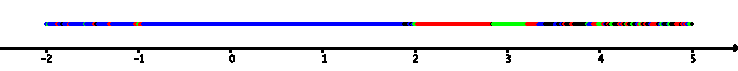
\includegraphics{figures/roots-order1}
\par\end{centering}
\begin{centering}
$f_{2}$: 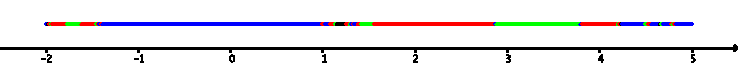
\includegraphics{figures/roots-order2}
\par\end{centering}
\begin{centering}
$f_{3}$: 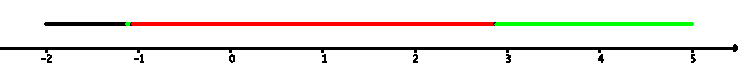
\includegraphics{figures/roots-order3}
\par\end{centering}
\begin{centering}
$f_{4}$: 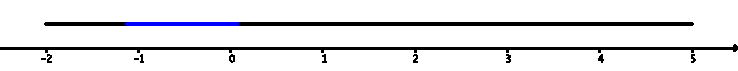
\includegraphics{figures/roots-order4}
\par\end{centering}
\begin{centering}
$f_{5}$: 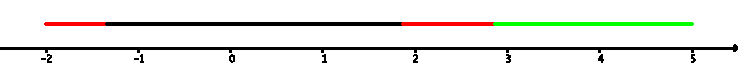
\includegraphics{figures/roots-order5}
\par\end{centering}
\centering{}hitam: tidak konvergen; hijau: konvergen ke $3$; merah:
konvergen ke $1+\sqrt{3}$; biru: konvergen ke $1-\sqrt{3}$
\end{figure}


\subsection{Metode Steffensen (kode semu)\index{metode Steffensen!kode semu}}

Karena metode Steffensen sangat rentan terhadap galat titik-mengambang,
kita melakukan pemeriksaan awal terhadap kekonvergenan sebelum langkah
delta-kuadrat Aitken. Hal ini membantu mencegah galat besar atau pembagian
dengan nol pada Langkah 4.

\begin{pseudocode} 
\begin{description}
\item [{Asumsi:}] Iterasi titik tetap konvergen ke suatu titik tetap dari
$f$ dengan nilai awal $x_{0}$.
\item [{Masukan:}] Nilai awal $x_{0}$; fungsi $f$; akurasi yang diinginkan
$tol$; jumlah maksimum iterasi $N$.
\item [{Langkah~1:}] Untuk $j=1\ldots N$ lakukan Langkah 2-6:

\begin{description}
\item [{Langkah~2:}] Tetapkan $x_{1}=f(x_{0})$; $x_{2}=f(x_{1})$
\item [{Langkah~3:}] Jika $|x_{2}-x_{1}|\leq tol$ maka kembalikan $x_{2}$
\item [{Langkah~4:}] Tetapkan $x=x_{0}-\frac{(x_{1}-x_{0})^{2}}{x_{2}-2x_{1}+x_{0}}$
\item [{Langkah~5:}] Jika $|x-x_{2}|\leq tol$ maka kembalikan $x$;
\item [{Langkah~6:}] Tetapkan $x_{0}=x$;
\end{description}
\item [{Langkah~7:}] Cetak ``Metode gagal. Jumlah iterasi maksimum terlampaui.''
\item [{Keluaran:}] Hampiran $x$ yang mendekati titik tetap eksak atau
pesan kegagalan.
\end{description}
\end{pseudocode}  

\subsection{Konsep Utama}
\begin{description}
\item [{Metode~delta-kuadrat~Aitken:}] Jika $\langle p_{n}\rangle$ konvergen
secara linear ke $p$, barisan $\langle a_{n}\rangle$ yang didefinisikan
oleh $a_{n}=p_{n}-\frac{(p_{n+1}-p_{n})^{2}}{p_{n+2}-2p_{n+1}+p_{n}}$
konvergen lebih cepat ke $p$, tetapi tetap berorde linear.
\item [{Batas~Galat~Titik~Tetap:}] \index{Teorema!Batas Galat Titik Tetap}
Misalkan $f$ adalah fungsi terdiferensial yang memiliki titik tetap
$\hat{x}$ dan misalkan $[a,b]$ adalah interval yang memuat $\hat{x}$.
 Jika $|f'(x)|\leq M<1$ untuk setiap $x\in[a,b]$ dan $f([a,b])\subseteq[a,b]$,
maka untuk sembarang nilai awal $x_{0}\in[a,b]$, iterasi titik tetap
dengan $x_{k+1}=f(x_{k})$ untuk setiap $k\geq0$ menghasilkan hampiran
terhadap $\hat{x}$ dengan galat absolut tidak lebih dari $M^{k}|x_{0}-\hat{x}|$.
\item [{Orde~Kekonvergenan~untuk~Iterasi~Titik~Tetap:}] Misalkan $f$
adalah fungsi dengan titik tetap $\hat{x}$ dan $f'(\hat{x})$ ada.
Misalkan $x_{0},x_{1},x_{2},\ldots$ merupakan barisan yang diperoleh
dari iterasi titik tetap ($x_{k+1}=f(x_{k})$ untuk setiap $k\geq1$)
sedemikian sehingga ${\displaystyle \lim_{k\to\infty}x_{k}=\hat{x}}$
dan $x_{k}\neq\hat{x}$ untuk setiap $k=0,1,2,\ldots$. Maka barisan
$\langle x_{n}\rangle$ konvergen secara linear ke $\hat{x}$ jika
$f'(\hat{x})\neq0$ dan berorde setidaknya kuadratik jika $f'(\hat{x})=0$.
\item [{Metode~Steffensen:}] \index{metode Steffensen}Modifikasi iterasi
titik tetap dengan setiap suku ketiga dihitung menggunakan metode
delta-kuadrat Aitken.
\item [{Kekonvergenan~superlinear:}] \index{kekonvergenan!superlinear}
Jika barisan $p_{0},p_{1},p_{2},\ldots$ konvergen ke $p$ dan ${\displaystyle \lim_{k\to\infty}\frac{|p_{k+1}-p|}{|p_{k}-p|}=0}$,
maka barisan tersebut dikatakan konvergen secara superlinear.
\item [{Kekonvergenan~superkuadratik:}] \index{kekonvergenan!superkuadratik}
Jika barisan $p_{0},p_{1},p_{2},\ldots$ konvergen ke $p$ dan ${\displaystyle \lim_{k\to\infty}\frac{|p_{k+1}-p|}{|p_{k}-p|^{2}}=0}$,
maka barisan tersebut dikatakan konvergen secara superkuadratik.
\end{description}

\subsection{Octave\label{subsec:WhileLoop}}

Pada Bagian \ref{sec:Speed}, kita telah mempelajari perulangan \texttt{for}.
Dengan perulangan \texttt{for}, Anda harus mengetahui berapa kali
perulangan itu hendak dijalankan, atau setidaknya menentukan jumlah
maksimum. Anda dapat menghentikan perulangan \texttt{for} sebelum
selesai dengan keluar (mengembalikan nilai) dari fungsi. Namun, adakalanya
Anda tidak tahu berapa kali perulangan perlu dijalankan dan bahkan
tidak memiliki batas maksimum yang sesuai. Dalam kasus ini, perulangan
\texttt{while} \index{Octave!perulangan while@perulangan \texttt{while}}
lebih tepat. Perulangan \texttt{while} akan terus berulang selama
kondisi tertentu terpenuhi; Anda sendiri yang menentukan kondisi tersebut.
Sintaks perulangan while adalah \begin{verbatim}
while (condition)
  do something. 
end%while
\end{verbatim}, tetapi harus digunakan dengan hati-hati. \texttt{for} selalu memiliki
akhir, tetapi perulangan \texttt{while} bisa tidak berakhir jika diprogram
dengan ceroboh. Jika \texttt{condition} pada perulangan \texttt{while}
tidak pernah terpenuhi, perulangan akan berjalan tanpa henti! Berikut
contoh sederhana perulangan \texttt{while} yang tidak pernah berakhir.
Jangan jalankan! \begin{verbatim}
i=0;
while (i<12)
  disp("Help! I'm stuck in a never-ending loop!!")
end%while
\end{verbatim} Masalahnya, \texttt{i} ditetapkan kurang dari 12 dan tidak pernah
berubah, sehingga selalu tetap kurang dari 12. Dengan demikian, kondisi
perulangan \texttt{while} ini selalu terpenuhi. Perulangan ini dapat
dengan mudah diubah agar berhenti. Jika kita menaikkan \texttt{i}
di dalam perulangan, perulangan tersebut akan berakhir. Modifikasi
terhadap perulangan tanpa akhir ini benar-benar berakhir dan menampilkan
pesan sebanyak 12 kali: \begin{verbatim}
i=0;
while (i<12)
  disp("That's better. I can handle a dozen iterations.")
  i=i+1;
end%while
\end{verbatim} Sebagai catatan, setiap perulangan \texttt{for} dapat digantikan
oleh perulangan \texttt{while} seperti yang satu ini. 

Kita adalah manusia. Tak terelakkan, suatu saat kita akan memprogram
perulangan while yang tidak pernah berakhir. Apa yang harus dilakukan
setelah perulangan itu mulai berjalan? Tentu saja, Anda dapat mematikan
komputer, tetapi itu seperti membawa cangkir kopi ke dapur dengan
buldoser. Ada cara yang lebih mudah. Anda cukup menghentikan aplikasi
tempat Octave sedang dijalankan. Jika menggunakan jendela baris perintah
(terminal) atau GUI Octave, Anda cukup menutupnya. Namun, jika masih
ingat, Anda juga dapat menekan \texttt{Ctrl-c}. Artinya, tekan tombol
\texttt{c} sambil menahan tombol \texttt{Ctrl}. Tindakan ini akan
menghentikan perulangan tanpa akhir tersebut.

Untuk contoh yang lebih praktis, metode bagi dua dapat dengan mudah
diprogram ulang menggunakan perulangan while. Pertama, kode semunya:

\begin{pseudocode} 
\begin{description}
\item [{Asumsi:}] $f$ kontinu pada $[a,b]$. $f(a)$ dan $f(b)$ memiliki
tanda yang berlawanan.
\item [{Masukan:}] Interval $[a,b]$; fungsi $f$; akurasi yang diinginkan
$tol$.
\item [{Langkah~1:}] Tetapkan $m=a$; $err=|b-a|$; $L=f(a)$;
\item [{Langkah~2:}] Selama $err>tol$, lakukan Langkah 3-5:

\begin{description}
\item [{Langkah~3:}] Tetapkan $m=\frac{a+b}{2}$; $M=f(m)$; $err=err/2$;
\item [{Langkah~4:}] Jika $M=0$ maka kembalikan $m$;
\item [{Langkah~5:}] Jika $LM<0$ maka tetapkan $b=m$; jika tidak, tetapkan
$a=m$ dan $L=M$;
\end{description}
\item [{Langkah~6:}] Kembalikan $m$.
\item [{Keluaran:}] Hampiran $m$ yang berjarak tidak lebih dari $tol$
dari akar eksak.
\end{description}
\end{pseudocode}  

\noindent Sekarang kode Octave-nya. Jika Anda memutuskan untuk menggunakan
kode ini, kode tersebut harus disimpan dalam berkas bernama \texttt{bisectionWhile.m}.

\begin{verbatim}
function p = bisectionWhile(a,b,f,tol)
  p = a;
  err = abs(b-a);
  FA = f(a);
  while (err>tol)
    p = a + (b-a)/2;
    FP = f(p);
    err=err/2;
    if (FP == 0)
      return
    end%if
    if (FA*FP > 0)
      a = p;
      FA = FP;
    else
      b = p;
    end%if
  end%while
end%function 
\end{verbatim} Gunakan kode ini dengan hati-hati! Kode ini dapat berjalan dalam
perulangan tak berujung! Jika fungsi dipanggil dengan nilai negatif
untuk \texttt{tol}, seperti dalam \texttt{bisectionWhile(g,1,2,-10)},
kode ini akan berjalan hingga dihentikan secara paksa (dengan \texttt{Ctrl-c}
atau dengan menutup aplikasi Octave), karena \texttt{err} akan selalu
lebih besar daripada $-10$.

\subsubsection{Pemeriksaan galat}

Perangkat lunak yang paling berguna menyertakan pemeriksaan galat.
Untuk fungsi \texttt{bisectionWhile} tersebut, kita ingin menghindari
perulangan tak berujung dalam setiap keadaan yang dapat kita bayangkan.
Menambahkan beberapa baris pada awal fungsi memberikan perlindungan:
\begin{verbatim}
function p = bisectionWhile(a,b,f,tol)
  if (tol<=0)
    p = "ERROR:tol must be positive.";
    return
  end%if
  p = a;
  err = abs(b-a);
  FA = f(a);
  while (err>tol)
    p = a + (b-a)/2;
    FP = f(p);
    err=err/2;
    if (FP == 0)
      return
    end%if
    if (FA*FP > 0)
      a = p;
      FA = FP;
    else
      b = p;
    end%if
  end%while
end%function 
\end{verbatim}

Secara umum, tindakan meminta program memeriksa galat masukan seperti
ini disebut pemeriksaan galat \index{pemeriksaan galat} atau validasi
\index{validasi}. Pada umumnya, kita akan menulis kode dengan mengasumsikan
bahwa masukannya valid dan tidak melakukan pemeriksaan galat. Ini
menyederhanakan pemrograman, tetapi juga memungkinkan timbulnya masalah
seperti perulangan tak berujung! \texttt{bisectionWhile.m} dapat diunduh
dari \href{http://lqbrin.github.io/tea-time-numerical/ancillaries.html}{situs pendamping}.

\startexercises 

\subsection{Latihan}
\begin{enumerate}
\item Berikan bukti bahwa $x_{k}\in[a,b]$ untuk setiap $k\geq0$ dalam
proposisi \ref{prop:fixedPointErrorBound}.
\item Tunjukkan bahwa 
\[
{\displaystyle \frac{p_{n+2}p_{n}-p_{n+1}^{2}}{p_{n+2}-2p_{n+1}+p_{n}}}
\]
dan 
\[
{\displaystyle p_{n}-\frac{(p_{n+1}-p_{n})^{2}}{p_{n+2}-2p_{n+1}+p_{n}}}
\]
ekuivalen secara aljabar.
\item \octave\ Tulislah fungsi Octave yang mengimplementasikan metode Steffensen.
\item \octave\ Tulislah program Octave (berkas \texttt{.m}) yang menggunakan
perulangan \texttt{ while} dan perintah \texttt{disp()} untuk menampilkan
10 hasil pemangkatan pertama dari 5, dimulai dengan $5^{0}$.
\item \label{exc:orderOfConvergence}\octave\ Tulislah program Octave (berkas
\texttt{.m}) yang menggunakan perulangan \texttt{while}, sebuah larik,
dan perintah \texttt{disp()} untuk menghitung nilai ${\displaystyle f(n)=\frac{2^{2^{n}}-2}{2^{2^{n}}+3}}$
untuk $n=0,1,2,4,6,10$. \hasasolution 
\item \octave\ Tulislah program Octave (berkas \texttt{.m}) yang menggunakan
perulangan \texttt{while}, sebuah larik, dan perintah \texttt{disp()}
untuk menghitung nilai ${\displaystyle f(n)=\frac{2n}{\sqrt{n^{2}+3n}}}$
untuk $n=0,2,5,10,100,1000,20000$.
\item \octave\ Kode Octave berikut dimaksudkan untuk menghitung jumlah
\[
\sum_{k=1}^{30}\frac{1}{k^{2}}
\]
, tetapi tidak berhasil melakukannya. Temukan sebanyak mungkin kesalahan
dalam kode tersebut. Klasifikasikan setiap kesalahan sebagai galat
kompilasi (galat yang akan membuat program sama sekali tidak dapat
dijalankan) atau galat logika (galat yang tidak mencegah program berjalan,
tetapi menyebabkan jumlah tersebut dihitung secara keliru).

\begin{lyxcode}
sum=1;~\\
k=1;~\\
while~k<30~\\
~~sum=sum+1.0/k{*}k;~\\
end~\\
diss(sum)
\end{lyxcode}
\item \octave\ Tulislah perulangan \texttt{while} yang menampilkan barisan
bilangan berikut.

\begin{enumerate}
\item $7,8,9,10,11,12,13,14,15$
\item \label{exc:orderOfConvergence-1}$20,19,18,17,16,15,14,13$ 
\item $12,12.333,12.667,13,13.333,13.667,14$
\item $1,9,25,49,81,121,169,225,289,361,441$
\item $1,.5,.25,.125,.0625,.03125,.015625$
\end{enumerate}
\item Fungsi $g(x)=\sqrt[3]{5-3x}$ memenuhi hipotesis proposisi \ref{prop:fixedPointErrorBound}
pada interval $[1,1.3]$. Tentukan batas bagi banyaknya iterasi yang
diperlukan untuk menentukan titik tetap dengan ketelitian $10^{-5}$
dengan nilai awal $x_{0}$ yang Anda pilih.
\item \label{exc:orderOfConvergence-2}Iterasi titik tetap pada fungsi $g(x)=\sqrt[3]{x^{2}+x}$
akan konvergen ke sekitar $1.618033988749895$ untuk setiap $x_{0}$
dalam $[0.5,3.5]$. \hasananswer 

\begin{enumerate}
\item Tentukan batas bagi banyaknya iterasi yang diperlukan untuk mencapai
ketelitian $10^{-4}$ dengan $x_{0}=2.5.$
\item Berapa banyak iterasi yang sebenarnya diperlukan untuk mencapai ketelitian
$10^{-4}$ dengan $x_{0}=2.5$?
\end{enumerate}
\item \label{exc:orderOfConvergence-3}Misalkan $f(x)=\frac{3x^{2}\text{\textminus}1}{6x+4}$.
Dalam latihan \ref{exc:fixedpt-12} pada bagian \ref{sec:Fixedpt},
Anda diminta menunjukkan bahwa $f$ memiliki titik tetap tunggal pada
$[-4,-0.9]$. \hasasolution 

\begin{enumerate}
\item Tentukan batas bagi banyaknya iterasi yang diperlukan untuk menghampiri
titik tetap dengan ketelitian $10^{-11}$, menggunakan iterasi titik
tetap dengan sembarang nilai awal dalam $[-4,-0.9]$. 
\item Gunakan iterasi titik tetap dengan $x_{0}=-4$ untuk memperoleh hampiran
titik tetap yang akurat hingga $10^{-11}$. Titik tetapnya adalah
$x=-1$.
\item Bandingkan batas tersebut dengan banyaknya iterasi yang sebenarnya
diperlukan.
\end{enumerate}
\item Misalkan $g(x)=\pi+0.5\sin(x/2)$. Dalam latihan \ref{enu:ShowPart2}
pada bagian \ref{sec:Fixedpt}, Anda diminta menunjukkan bahwa $g$
memiliki titik tetap tunggal pada $[0,2\pi]$.

\begin{enumerate}
\item Tentukan batas bagi banyaknya iterasi yang diperlukan untuk mencapai
ketelitian $10^{-2}$, menggunakan iterasi titik tetap dengan sembarang
nilai awal dalam $[0,2\pi]$. 
\item Gunakan iterasi titik tetap dengan $x_{0}=0$ untuk mencari hampiran
titik tetap dengan galat tidak lebih dari $10^{-2}$. Titik tetapnya
adalah $x=???$.
\item Bandingkan batas tersebut dengan banyaknya iterasi yang sebenarnya
diperlukan.
\end{enumerate}
\item \label{exc:orderOfConvergence-4}Hitung dua iterasi metode Steffensen
untuk $g(x)=\sqrt[3]{x^{2}+x}$ dengan $x_{0}=2.5$.  \hasananswer 
\item \label{exc:orderOfConvergence-5}Gunakan metode Steffensen untuk mencari
akar $g(x)=x^{4}-2x^{3}-4x^{2}+4x+4$ dalam interval $[2,3]$ dengan
ketelitian lima angka signifikan. \hasananswer 
\item \label{enu:aitkensOnSequence}Hitung $a_{0},a_{1},$ dan $a_{2}$
dari metode delta-kuadrat Aitken untuk barisan pada soal \ref{enu:linearConvergenceExample}
\vpageref{enu:linearConvergenceExample}. Karena barisan tersebut
memiliki suku yang tidak terdefinisi pada $n=1$, mulailah barisan
$\langle\frac{n+1}{n-1}\rangle$ dari $n=2$. Dengan kata lain, anggap
barisan pada soal \ref{enu:linearConvergenceExample} \vpageref{enu:linearConvergenceExample}
sebagai $3,2,\frac{5}{3},\frac{3}{2},\frac{7}{5}\ldots$ sehingga
$p_{0}=3$, $p_{1}=2$, $p_{2}=\frac{5}{3}$, dan seterusnya.
\item Barisan-barisan berikut konvergen secara linear. Bangkitkan lima suku
pertama barisan $\langle a_{n}\rangle$ menggunakan perhitungan delta-kuadrat
Aitken.

\begin{enumerate}
\item \label{exc:orderOfConvergence-6}$p_{0}=0.5$, $p_{n}=(2-e^{p_{n-1}}+p_{n-1}^{2})/3$
untuk $n\geq1$ \hasasolution 
\item $p_{0}=0.75$, $p_{n}=\sqrt{e^{p_{n-1}}/3}$ untuk $n\geq1$
\end{enumerate}
\item Gunakan metode delta-kuadrat Aitken untuk mencari ${\displaystyle p=\lim_{n\to\infty}p_{n}}$
dengan ketelitian 3 tempat desimal.
\begin{align*}
p_{n} & =\{-2,\ -1.85271,\ -1.74274,\ -1.66045,\\
 & \qquad-1.59884,\ -1.55266,\ -1.51804,\ \\
 & \qquad-1.49208,\ -1.47261,\ \ldots\}
\end{align*}
\item \label{exc:orderOfConvergence-7}Barisan $\langle a_{n}\rangle$ pada
soal \ref{enu:aitkensOnSequence} konvergen lebih cepat daripada barisan
pada soal \ref{enu:linearConvergenceExample} \vpageref{enu:linearConvergenceExample}.
Jika metode delta-kuadrat Aitken diterapkan pada barisan $\langle a_{n}\rangle$,
apakah Anda memperkirakan konvergensinya akan lebih cepat lagi? Jelaskan. \hasananswer 
\item Ingat kembali dari kalkulus bahwa $\lim_{n\to\infty}n\sin\left(\frac{1}{n}\right)=1$.
Oleh karena itu, jika kita menetapkan $p_{n}=n\sin\left(\frac{1}{n}\right)$,
maka barisan $\langle p_{1},p_{2},p_{3},\ldots\rangle\approx\langle.84147,.95885,.98158,\ldots\rangle$
konvergen ke 1, meskipun sangat lambat. Bangkitkan tiga suku pertama
barisan $\langle a_{n}\rangle$ menggunakan perhitungan delta-kuadrat
Aitken. Apakah barisan itu tampak mendekati 1 lebih cepat daripada
$\langle p_{n}\rangle$?
\item \label{exc:orderOfConvergence-8}Iterasi titik tetap yang diterapkan
pada $f(x)=\sin(x)$ dengan $x_{0}=1$ memerlukan $29,992$ iterasi
untuk mencapai bilangan di bawah $0.01$ ketika menuju titik tetap
$0$. Kebetulan, $x_{29992}\approx0.099999$. Berapa iterasi yang
diperlukan metode Steffensen dengan $x_{0}=1$ untuk mencapai bilangan
di bawah $0.01$? Berikan komentar. \hasasolution 
\item \label{exc:orderOfConvergence-9}Misalkan $f(x)=1+(\sin x)^{2}$ dan
$p_{0}=1$. Dengan kalkulator, hitung $a_{1}$ dan $a_{2}$ dari metode
Steffensen. \hasananswer 
\item Hitung tiga iterasi pertama metode Steffensen yang diterapkan pada
$g(x)=(\sqrt{2})^{x}$ dengan $p_{0}=3$.
\item \label{exc:orderOfConvergence-10}Metode Steffensen diterapkan pada
fungsi $f(x)$ dengan $p_{0}=1$. Jika $f(f(p_{0}))=3$ dan $a_{1}=0.75$,
berapakah $f(p_{0})$? \hasananswer 
\item \label{Steffensens}Cari titik tetap $f(x)=x-0.002(e^{x}\cos(x)-100)$
dalam interval $[5,6]$ menggunakan metode Steffensen. \hasananswer 
\item Dalam soal \ref{Steffensens} Anda menemukan suatu titik tetap $\hat{x}$.
Fungsi $g(x)$ apakah yang memiliki $\hat{x}$ sebagai akar?
\item \octave\ Tulislah perulangan \texttt{while} yang menampilkan bilangan-bilangan
$1,.5,.25,.125,.0625,.03125,.015625,\ldots$ hingga mencapai suatu
bilangan yang lebih kecil daripada $10^{-4}$.
\end{enumerate}
\finishexercises

\section{\label{sec:newtonsMethod}Metode Newton\index{metode Newton}\index{metode!Newton|see{metode Newton}}}

Pada bagian \ref{sec:fixedptOrder}, kita membahas sebagian kekurangan
iterasi titik tetap, tetapi menunda pembahasan mendalam tentang fungsi
misterius $f_{6}$ dari penyelidikan pencarian akar \vpageref{subsec:RootFindingInvestigation}.
Kini saatnya membahas $f_{6}$ secara lebih terperinci. Kita mulai
dengan beberapa perhitungan numerik. Ingat bahwa $f_{6}(x)=\frac{2x^{3}\text{\textminus}5x^{2}\text{\textminus}6}{3x^{2}\text{\textminus}10x+4}$
dan tetapkan $x_{0}=4.$ Dengan melanjutkan iterasi titik tetap,
\begin{eqnarray*}
x_{1}=f_{6}(x_{0}) & = & 3.5\\
x_{2}=f_{6}(x_{1}) & \approx & 3.217391304347826\\
x_{3}=f_{6}(x_{2}) & \approx & 3.072749058541597\\
x_{4}=f_{6}(x_{3}) & \approx & 3.013730618589344\\
x_{5}=f_{6}(x_{4}) & \approx & 3.000683798275568\\
x_{6}=f_{6}(x_{5}) & \approx & 3.000001860777997\\
x_{7}=f_{6}(x_{6}) & \approx & 3.000000000013848.
\end{eqnarray*}
Anda dapat melihat dua hal. Barisan $x_{0},x_{1},x_{2},\ldots$
\begin{enumerate}
\item konvergen ke (titik tetap) 3; dan
\item tampaknya kekonvergenannya kuadratik karena, sejak peralihan dari
$x_{4}$ ke $x_{5}$, jumlah angka signifikan kira-kira berlipat dua
pada setiap iterasi.
\end{enumerate}
Dalam analisis pada bagian \ref{sec:fixedptOrder} \vpageref{sec:fixedptOrder},
kita menemukan bahwa iterasi titik tetap konvergen secara kuadratik
(atau lebih cepat) hanya ketika turunan di titik tetap bernilai nol.
Pengamatan ini semestinya membuat Anda menduga bahwa $f_{6}'(3)=0$.
Mari kita periksa. Pertama, turunannya adalah $f_{6}'(x)=\frac{6x^{4}\text{\textminus}40x^{3}+74x^{2}\text{\textminus}4x\text{\textminus}60}{(3x^{2}\text{\textminus}10x+4)^{2}}$
(Anda sebaiknya memverifikasi ini). Dengan mengevaluasi pembilang
di titik tetap, $x=3$, kita memperoleh $6(3)^{4}-40(3)^{3}+74(3)^{2}-4(3)-60=486-1080+666-12-60=0$.
Jadi, kita memperoleh kekonvergenan menuju titik tetap tempat turunan
fungsi bernilai nol, dan memang kekonvergenannya kuadratik.

Dengan $x_{0}=2$ sebagai nilai awal, iterasi titik tetap pada $f_{6}$
konvergen ke $1+\sqrt{3}$, sedangkan dengan $x_{0}=-1$ sebagai nilai
awal, iterasi titik tetap konvergen ke $1-\sqrt{3}$. Anda seharusnya
dapat memverifikasi hal ini dari diagram kekonvergenan pada Gambar
\ref{fig:SixConvergenceDiagrams} atau dengan menghitung sendiri beberapa
iterasi pertama untuk masing-masing kasus. Yang tidak ditunjukkan
oleh diagram kekonvergenan adalah laju kekonvergenannya. Untuk itu,
Anda perlu melihat hasil-hasil iterasinya. Silakan lakukan. Apakah
kekonvergenannya juga tampak kuadratik dalam kasus-kasus ini? Jawaban
\vpageref{que:quadraticConvergence}.

Dari diagram kekonvergenan, kita melihat bahwa iterasi titik tetap
akan konvergen untuk hampir semua nilai awal, dan ketiga titik tetap
dapat dihampiri dengan iterasi titik tetap. Selain itu, dari perhitungan
kita, tampaknya kekonvergenannya kuadratik untuk ketiganya. Sulit
mengharapkan lebih banyak dari suatu fungsi. Kekonvergenan yang cepat
menuju titik tetap mana pun! Jadi, dari mana $f_{6}$ berasal?

Misalkan $g(x)$ terdiferensialkan dan $g(\hat{x})=0$, sehingga $g$
memiliki akar di $\hat{x}$. Tinjau $f(x)=x-\frac{g(x)}{g'(x)}$.
$\hat{x}$ merupakan titik tetap $f$ selama $g'(\hat{x})\neq0$:
\[
f(\hat{x})=\hat{x}-\frac{g(\hat{x})}{g'(\hat{x})}=\hat{x}-\frac{0}{g'(\hat{x})}=\hat{x}.
\]
Selain itu, selama $g$ memiliki turunan kedua di sekitar $\hat{x}$,
\begin{eqnarray*}
f'(\hat{x}) & = & 1-\frac{g'(\hat{x})\cdot g'(\hat{x})-g(\hat{x})g''(\hat{x})}{g'(\hat{x})\cdot g'(\hat{x})}\\
 & = & 1-1+\frac{0\cdot g''(\hat{x})}{g'(\hat{x})\cdot g'(\hat{x})}\\
 & = & 0.
\end{eqnarray*}
Dari perhitungan ini, kita menyimpulkan bahwa jika $g(x)$ terdiferensialkan
dua kali, $g(\hat{x})=0$ dan $g'(\hat{x})\neq0$, maka iterasi titik
tetap untuk $f(x)$ dengan nilai awal di suatu lingkungan $\hat{x}$
akan konvergen secara kuadratik ke $\hat{x}$. Sungguh cara yang hebat
untuk mengubah masalah pencarian akar menjadi masalah titik tetap!

Sekarang saat yang tepat untuk mengingat bahwa $f_{6}$ hanyalah salah
satu dari 6 fungsi kandidat yang dirancang untuk mencari akar dari
$g(x)=-x^{3}+5x^{2}-4x-6$ dengan iterasi titik tetap. Memang, $g'(x)=-3x^{2}+10x-4$
dan 
\begin{eqnarray*}
x-\frac{g(x)}{g'(x)} & = & x-\frac{-x^{3}+5x^{2}-4x-6}{-3x^{2}+10x-4}\\
 & = & \frac{2x^{3}\text{\textminus}5x^{2}\text{\textminus}6}{3x^{2}\text{\textminus}10x+4}\\
 & = & f_{6}(x).
\end{eqnarray*}
Penggunaan iterasi titik tetap pada $f_{6}(x)=x-\frac{g(x)}{g'(x)}$
untuk mencari akar $g(x)$, seperti yang dilakukan di sini, disebut
\index{metode Newton} metode Newton.

\subsection{Penurunan Geometris Metode Newton}

\noindent Gambar berikut menunjukkan cara menghitung dua iterasi pertama
metode Newton pada $g(x)=-x^{3}+5x^{2}-4x-6$ dengan nilai awal $x_{0}=-2.5$
secara geometris.

\begin{center}
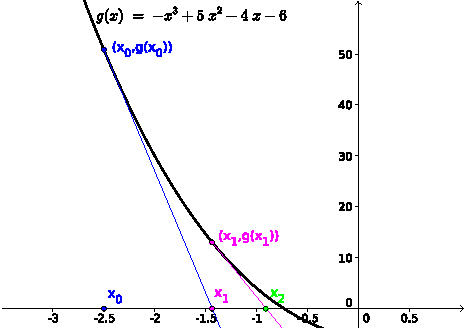
\includegraphics{figures/roots-newton1}\label{img:newtonsMethod}
\par\end{center}

\noindent Untuk menghitung $x_{1}$, tarik garis singgung pada $g$
di $(x_{0},g(x_{0}))$; perpotongan garis ini dengan sumbu $x$ adalah
$x_{1}$. Demikian pula, tarik garis singgung pada $g$ di $(x_{1},g(x_{1}))$;
perpotongan garis ini dengan sumbu $x$ adalah $x_{2}$. Demikian
seterusnya. Sebagai contoh, $(x_{0},g(x_{0}))=(-2.5,50.875)$ dan
$g'(x_{0})=g'(-2.5)=-47.75$. Oleh karena itu, ``perubahan vertikal''
($0-50.875$) dibagi ``perubahan horizontal'' ($x_{1}+2.5$) antara
$(-2.5,50.875)$ dan $(x_{1},0)$ harus sama dengan $-47.75$. Dengan
demikian, kita memperoleh $\frac{-50.875}{x_{1}+2.5}=-47.75$ sehingga
\[
x_{1}=\frac{-50.875}{-47.75}-2.5\approx-1.43455497382199.
\]
Dalam simbol, ``perubahan vertikal'' ($-g(x_{0})$) dibagi ``perubahan
horizontal'' ($x_{1}-x_{0})$ harus sama dengan $g'(x_{0})$. Dengan
kata lain,
\begin{eqnarray*}
\frac{-g(x_{0})}{x_{1}-x_{0}} & = & g'(x_{0})\Rightarrow\\
\frac{-g(x_{0})}{g'(x_{0})} & = & x_{1}-x_{0}\Rightarrow\\
x_{1} & = & x_{0}-\frac{g(x_{0})}{g'(x_{0})}.
\end{eqnarray*}
Perhitungan serupa menunjukkan $x_{2}=x_{1}-\frac{g(x_{1})}{g'(x_{1})}$,
dan secara lebih umum $x_{n+1}=x_{n}-\frac{g(x_{n})}{g'(x_{n})}$.
Relasi rekurensi ini menjelaskan metode Newton---yakni mengiterasikan
fungsi $f(x)=x-\frac{g(x)}{g'(x)}$.

\subsection{Metode Newton (kode semu)\index{metode Newton!kode semu}}

Tidak seperti pada metode Steffensen, penyebut dalam metode Newton
tidak diharapkan mendekati nol ketika hasil-hasil iterasinya konvergen;
karena itu, secara umum kestabilan perhitungan jauh lebih jarang bermasalah
dan tidak dilakukan pemeriksaan perantara sebelum menghitung satu
iterasi dari iterasi sebelumnya.

\begin{pseudocode} 
\begin{description}
\item [{Asumsi:}] $g$ terdiferensialkan dua kali. $g$ memiliki akar di
$\hat{x}$. $x_{0}$ berada dalam lingkungan $(\hat{x}-\delta,\hat{x}+\delta)$
tempat nilai mutlak $f'(x)=1-\frac{g'(x)\cdot g'(x)-g(x)g''(x)}{g'(x)\cdot g'(x)}$
kurang dari satu.
\item [{Masukan:}] Nilai awal $x_{0}$; fungsi $g$ beserta turunannya
$g'$; akurasi yang diinginkan $tol$; jumlah iterasi maksimum $N$.
\item [{Langkah~1:}] Untuk $j=1\ldots N$ lakukan Langkah 2--4:

\begin{description}
\item [{Langkah~2:}] Tetapkan $x=x_{0}-\frac{g(x_{0})}{g'(x_{0})}$;
\item [{Langkah~3:}] Jika $|x-x_{0}|\leq tol$ maka kembalikan $x$;
\item [{Langkah~4:}] Tetapkan $x_{0}=x$;
\end{description}
\item [{Langkah~5:}] Cetak ``Metode gagal. Jumlah iterasi maksimum terlampaui.''
\item [{Keluaran:}] Hampiran $x$ di dekat titik tetap eksak, atau pesan
kegagalan.
\end{description}
\end{pseudocode}  

\subsection{Metode Sekan\index{metode sekan}\index{metode!sekan|see{metode sekan}}}

Kelemahan terbesar metode Newton adalah keharusan untuk mengetahui
$g'$ dan menggunakannya dalam perhitungan. Namun, turunan tidak selalu
tersedia, mudah ditangani, atau bahkan diketahui. Dalam kasus seperti
itu, lebih baik menggunakan metode Steffensen atau metode sekan. Metode
sekan diturunkan dengan mengganti $g'$ dalam metode Newton dengan
hasil bagi selisih. Agar penggantian ini masuk akal, kita perlu menyatakan
kembali metode Newton dalam bentuk $x_{n}$. Dalam metode Newton,
kita mengiterasikan $f(x)=x-\frac{g(x)}{g'(x)}$ sehingga $x_{n+1}=x_{n}-\frac{g(x_{n})}{g'(x_{n})}$.

Sekarang, misalkan Anda memiliki fungsi $g$ dan suatu hasil iterasi
$x_{n-1}$. Informasi ini cukup untuk menentukan satu titik pada grafik
$g$, yaitu $(x_{n-1},g(x_{n-1}))$. Namun, kita memerlukan satu titik
lagi untuk membentuk hasil bagi selisih (kemiringan garis yang melalui
dua titik). Maka, misalkan kita memiliki nilai kedua, $x_{n}$, yang
dekat dengan $x_{n-1}$. Maka, $\frac{g(x_{n})-g(x_{n-1})}{x_{n}-x_{n-1}}\approx g'(x_{n})$
sehingga kita dapat mengganti $\frac{g(x_{n})-g(x_{n-1})}{x_{n}-x_{n-1}}$
sebagai pengganti $g'(x_{n})$ dalam metode Newton. Penggantian ini
menghasilkan \index{metode sekan} metode sekan, $x_{n+1}=x_{n}-g(x_{n})/\left(\frac{g(x_{n})-g(x_{n-1})}{x_{n}-x_{n-1}}\right)$,
yang dapat disederhanakan menjadi
\begin{equation}
x_{n+1}=x_{n}-g(x_{n})\frac{x_{n}-x_{n-1}}{g(x_{n})-g(x_{n-1})}.\label{eq:secantMethod}
\end{equation}
Secara geometris, dapatkah Anda melihat cara kerja metode ini? Jawaban
\vpageref{que:secantMethodGeometrically}. Perhatikan bahwa ini tidak
sepenuhnya merupakan skema iterasi titik tetap. Setiap iterasi bergantung
pada \textit{dua} nilai sebelumnya, bukan satu. Analisis yang telah
kita lakukan sejauh ini tidak berlaku, tetapi ada harapan bahwa kekonvergenannya
akan cepat karena metode ini merupakan hampiran yang wajar terhadap
metode Newton di dekat suatu akar, dengan asumsi $g$ terdiferensialkan
di sekitar akar tersebut. Tabel 
\begin{table}
\hrule 

\caption{\label{tab:secantDemo} Metode sekan yang diterapkan pada $g(x)=-x^{3}+5x^{2}-4x-6$
dengan $x_{0}=5$ dan $x_{1}=x_{0}+g(x_{0})=-21$.}

\centering{}\medskip{}
\begin{tabular}{ccc}
$n$ & $x_{n}$ & $|3-x_{n}|$\tabularnewline
\hline 
0 & $5$ & $2(10)^{0}$\tabularnewline
1 & $-21$ & $2.4(10)^{1}$\tabularnewline
2 & $4.9415730337078$ & $1.941(10)^{0}$\tabularnewline
3 & $4.8869924815972$ & $1.886(10)^{0}$\tabularnewline
4 & $4.0502898397912$ & $1.050(10)^{0}$\tabularnewline
5 & $3.7088949488497$ & $7.088(10)^{-1}$\tabularnewline
6 & $3.412824115541$ & $4.128(10)^{-1}$\tabularnewline
7 & $3.232292913133$ & $2.322(10)^{-1}$\tabularnewline
8 & $3.1141957095727$ & $1.141(10)^{-1}$\tabularnewline
9 & $3.0465011115969$ & $4.650(10)^{-2}$\tabularnewline
10 & $3.0132833760752$ & $1.328(10)^{-2}$\tabularnewline
11 & $3.0020189248976$ & $2.018(10)^{-3}$\tabularnewline
12 & $3.0001014520965$ & $1.014(10)^{-4}$\tabularnewline
13 & $3.0000008128334$ & $8.128(10)^{-7}$\tabularnewline
14 & $3.0000000003297$ & $3.297(10)^{-10}$\tabularnewline
\end{tabular}\medskip{}
\hrule 
\end{table}
\ref{tab:secantDemo} memberikan bukti bahwa metode sekan memang konvergen
dengan cepat. Dalam kasus khusus $g(x)=-x^{3}+5x^{2}-4x-6$ dengan
$x_{0}=5$ dan $x_{1}=x_{0}+g(x_{0})=-21$, diperlukan beberapa saat
sampai perilakunya stabil, tetapi setelah kira-kira 8 iterasi pertama,
kekonvergenannya sangat cepat. Tidak sepenuhnya kuadratik, tetapi
jelas superlinear.

\begin{digression}{Metode sekan konvergen dengan orde $\frac{1+\sqrt{5}}{2}$.}

\noindent\index{metode sekan!analisis}Misalkan $g$ adalah fungsi
dengan akar $\hat{x}$, $g'(\hat{x})\neq0$, $g''(\hat{x})\neq0$,
dan $g'''(x)$ ada di suatu lingkungan $\hat{x}$. Misalkan $x_{0},x_{1},x_{2},\ldots$
adalah barisan yang diperoleh dari metode sekan ($x_{n+1}=x_{n}-g(x_{n})\frac{x_{n}-x_{n-1}}{g(x_{n})-g(x_{n-1})}$
untuk semua $k\geq2$) sedemikian sehingga ${\displaystyle \lim_{k\to\infty}x_{k}=\hat{x}}$.
Definisikan $e_{n}=x_{n}-\hat{x}$ sehingga $x_{n}=\hat{x}+e_{n}$.
Dengan melakukan substitusi ini ke dalam \ref{eq:secantMethod} kita
memperoleh 
\begin{equation}
e_{n+1}=e_{n}-g(\hat{x}+e_{n})\frac{e_{n}-e_{n-1}}{g(\hat{x}+e_{n})-g(\hat{x}+e_{n-1})}.\label{eq:secantOrderPart1}
\end{equation}
Teorema Taylor memberikan $g(\hat{x}+e_{k})=g(\hat{x})+e_{k}g'(\hat{x})+\frac{1}{2}e_{k}^{2}g''(\hat{x})+O(e_{k}^{3})$.
Dengan memperhatikan bahwa $g(\hat{x})=0$ dan mensubstitusikannya
ke dalam \ref{eq:secantOrderPart1},
\begin{eqnarray}
e_{n+1} & = & e_{n}-(e_{n}-e_{n-1})\frac{e_{n}g'(\hat{x})+\frac{1}{2}e_{n}^{2}g''(\hat{x})+O(e_{n}^{3})}{(e_{n}-e_{n-1})g'(\hat{x})+\frac{1}{2}(e_{n}^{2}-e_{n-1}^{2})g''(\hat{x})+O(e_{n-1}^{3})}\nonumber \\
 & = & e_{n}-\frac{e_{n}+\frac{e_{n}^{2}g''(\hat{x})}{2g'(\hat{x})}+O(e_{n}^{3})}{1+\frac{(e_{n}+e_{n-1})g''(\hat{x})}{2g'(\hat{x})}+\frac{O(e_{n-1}^{3})}{(e_{n}-e_{n-1})}}\nonumber \\
 & = & \frac{e_{n}\left(1+\frac{(e_{n}+e_{n-1})g''(\hat{x})}{2g'(\hat{x})}+\frac{O(e_{n-1}^{3})}{(e_{n}-e_{n-1})}\right)-\left(e_{n}+\frac{e_{n}^{2}g''(\hat{x})}{2g'(\hat{x})}+O(e_{n}^{3})\right)}{1+\frac{(e_{n}+e_{n-1})g''(\hat{x})}{2g'(\hat{x})}+\frac{O(e_{n-1}^{3})}{(e_{n}-e_{n-1})}}\nonumber \\
 & = & \frac{e_{n}e_{n-1}\frac{g''(\hat{x})}{2g'(\hat{x})}+\frac{e_{n}}{e_{n}-e_{n-1}}O(e_{n-1}^{3})+O(e_{n}^{3})}{1+\frac{(e_{n}+e_{n-1})g''(\hat{x})}{2g'(\hat{x})}+\frac{O(e_{n-1}^{3})}{(e_{n}-e_{n-1})}}.\label{eq:secantOrderPart2}
\end{eqnarray}
Dengan menggunakan persamaan \ref{eq:secantOrderPart2} untuk mencari
nilai $\alpha$ yang memenuhi $\lim_{n\to\infty}\frac{|\hat{x}-x_{n+1}|}{|\hat{x}-x_{n}|^{\alpha}}=\lambda\neq0$,
kita memperoleh
\begin{eqnarray*}
\lim_{n\to\infty}\frac{|\hat{x}-x_{n+1}|}{|\hat{x}-x_{n}|^{\alpha}} & = & \lim_{n\to\infty}\frac{|e_{n+1}|}{|e_{n}|^{\alpha}}\\
 & = & \lim_{n\to\infty}\left|\frac{e_{n}^{1-\alpha}e_{n-1}\frac{g''(\hat{x})}{2g'(\hat{x})}+\frac{e_{n}^{1-\alpha}}{e_{n}-e_{n-1}}O(e_{n-1}^{3})+O(e_{n}^{3-\alpha})}{1+\frac{(e_{n}+e_{n-1})g''(\hat{x})}{2g'(\hat{x})}+\frac{O(e_{n-1}^{3})}{(e_{n}-e_{n-1})}}\right|\\
 & = & \lambda\neq0.
\end{eqnarray*}
Namun, $\lim_{n\to\infty}e_{n}=\lim_{n\to\infty}e_{n-1}=0$. Oleh
karena itu, $\lim_{n\to\infty}e_{n}^{1-\alpha}e_{n-1}$ tidak boleh
bernilai 0 ataupun divergen, sebab jika demikian, $\lim_{n\to\infty}\frac{|\hat{x}-x_{n+1}|}{|\hat{x}-x_{n}|^{\alpha}}$
masing-masing akan bernilai 0 atau divergen. Akibatnya, terdapat konstanta
positif $C$ sedemikian sehingga $\lim_{n\to\infty}|e_{n}^{1-\alpha}e_{n-1}|=\lim_{n\to\infty}|e_{n+1}^{1-\alpha}e_{n}|=C\Rightarrow\lim_{n\to\infty}|e_{n+1}e_{n}^{1/(1-\alpha)}|=C^{1/(1-\alpha)}$.
Sekarang kita memperoleh 
\[
\lim_{n\to\infty}\frac{|e_{n+1}|}{|e_{n}|^{\alpha}}=\lambda\neq0\mbox{ dan }\lim_{n\to\infty}\frac{|e_{n+1}|}{|e_{n}|^{1/(\alpha-1)}}=C^{1/(1-\alpha)}\neq0.
\]
Karena orde kekonvergenan suatu barisan bersifat unik (Latihan \ref{enu:orderOfConvergenceIsUnique}
pada bagian \ref{sec:Speed}), haruslah $\alpha=1/(\alpha-1)$ atau
$\alpha^{2}-\alpha-1=0$. Rumus kuadrat memberikan hasil yang diinginkan.

\end{digression}

Sejauh ini kita baru menerapkan metode Newton dan metode sekan pada
polinom kubik $g(x)=-x^{3}+5x^{2}-4x-6$, suatu pekerjaan yang sebenarnya
tidak diperlukan. Teorema akar rasional, alat dasar dalam prakalkulus,
akan memungkinkan Anda memperoleh akar-akarnya secara eksak. Teorema
tersebut meminta Anda memeriksa $\pm1,\pm2,\pm3,$ dan $\pm6$ sebagai
akar-akar yang mungkin dari $g$. Dengan asumsi bahwa Anda melakukan
pemeriksaan menggunakan pembagian sintetis, perhitungan Anda mungkin
tampak seperti ini:\label{syntheticDivisionExample}

\begin{center}
\begin{tabular}{ccccc}
\multicolumn{1}{c|}{$3$} & $-1$ & $5$ & $-4$ & $-6$\tabularnewline
\cline{1-1}
 &  & $-3$ & $6$ & $6$\tabularnewline
\hline 
 & $-1$ & $2$ & \multicolumn{1}{c|}{$2$} & \multicolumn{1}{c|}{$0$}\tabularnewline
\cline{5-5}
\end{tabular}
\par\end{center}

\noindent yang berarti $g(x)=(x-3)(-x^{2}+2x+2)$. Dua akar lainnya
kemudian diperoleh dengan menerapkan rumus kuadrat pada $-x^{2}+2x+2$
dan hasilnya adalah $\frac{-2\pm\sqrt{4+8}}{-2}=1\pm\sqrt{3}$.

\noindent\begin{digression}{Menyelesaikan persamaan kubik}  

\noindent Akar-akar persamaan kuadrat $ax^{2}+bx+c=0$ diberikan oleh
rumus kuadrat yang sudah dikenal luas. Yang kurang dikenal, dan jauh
lebih rumit, adalah rumus untuk memperoleh akar-akar \index{rumus kubik}
persamaan kubik $ax^{3}+bx^{2}+cx+d=0$. Salah satu metode penyelesaiannya
adalah sebagai berikut. Pertama, kita tetapkan
\begin{eqnarray*}
p & = & \frac{3ac-b^{2}}{3a^{2}}\qquad\mbox{dan}\\
q & = & \frac{2b^{3}-9abc+27a^{2}d}{27a^{3}}.
\end{eqnarray*}
Kemudian kita tetapkan 
\[
w^{3}=-\frac{q}{2}-\sqrt{\frac{q^{2}}{4}+\frac{p^{3}}{27}}.
\]
Ketiga, kita tetapkan $w_{1},w_{2},$ dan $w_{3}$ sebagai tiga nilai
(kompleks) yang mungkin bagi $w$. Terakhir, ketiga penyelesaian $ax^{3}+bx^{2}+cx+d=0$
adalah 
\[
x_{i}=w_{i}-\frac{p}{3w_{i}}-\frac{b}{3a},\quad i=1,2,3.
\]
Ini pada dasarnya adalah metode \index{Cardano!rumus kubik} Cardano,
yang diterbitkan pada abad ke-$16$!

Sebagai contoh, untuk menyelesaikan persamaan $-x^{3}+5x^{2}-4x-6=0$,
kita mulai dengan
\begin{eqnarray*}
p & = & \frac{3(-1)(-4)-5^{2}}{3(-1)^{2}}=-\frac{13}{3}\qquad\mbox{dan}\\
q & = & \frac{2\cdot5^{3}-9(-1)(5)(-4)+27(-1)^{2}(-6)}{27(-1)^{3}}=\frac{92}{27}.
\end{eqnarray*}
Kemudian
\begin{eqnarray*}
w^{3} & = & -\frac{92}{2\cdot27}-\sqrt{\frac{92^{2}}{4\cdot27^{2}}-\frac{13^{3}}{27^{2}}}\\
 & = & -\frac{46}{27}-\frac{\sqrt{92^{2}-4\cdot13^{3}}}{54}\\
 & = & -\frac{46}{27}-\frac{\sqrt{-324}}{54}\\
 & = & -\frac{46}{27}-\frac{i}{3}.
\end{eqnarray*}
Dalam bentuk polar, $w^{3}=\frac{13\sqrt{13}}{27}e^{i(\tan^{-1}(9/46)-\pi)}$
sehingga kita dapat menetapkan $w_{1}=\frac{\sqrt{13}}{3}e^{i(\tan^{-1}(9/46)-\pi)/3}$,
salah satu akar pangkat tiga dari $w^{3}$. Sayangnya, menentukan
sudut $(\tan^{-1}(9/46)-\pi)/3$ secara eksak setara dengan menyelesaikan
persamaan kubik! Namun, dengan bantuan kalkulator, kita dapat memperoleh
hampiran $\text{\textminus}0.982793723247329$, yang pada akhirnya
cukup baik. Jadi, bagian real dari $w_{1}$ kira-kira $\frac{\sqrt{13}}{3}\cos(\text{\textminus}0.982793723247329)\approx.6666666666666667$
dan bagian imajinernya kira-kira $\frac{\sqrt{13}}{3}\sin(\text{\textminus}0.982793723247329)\approx-1$.
$w_{1}$ sangat dekat dengan $\frac{2}{3}-i$. Dan kita dapat memeriksa,
$\left(\frac{2}{3}-i\right)^{3}=\left(\frac{2}{3}\right)^{3}+3\left(\frac{2}{3}\right)^{2}(-i)+3\cdot\frac{2}{3}(-i)^{2}+(-i)^{3}=\frac{8}{27}-\frac{12}{9}i-2+i=-\frac{46}{27}-\frac{1}{3}i$.
Oleh karena itu, $w_{1}=\frac{2}{3}-i$ dan kita tetapkan $w_{2}=\left(\frac{2}{3}-i\right)\left(-\frac{1}{2}+\frac{\sqrt{3}}{2}i\right)=\frac{3\sqrt{3}-2}{6}+\frac{3+2\sqrt{3}}{6}i$
serta $w_{3}=\left(\frac{2}{3}-i\right)\left(-\frac{1}{2}-\frac{\sqrt{3}}{2}i\right)=\frac{-3\sqrt{3}-2}{6}+\frac{3-2\sqrt{3}}{6}i$.
Terakhir,
\begin{eqnarray*}
x_{1} & = & w_{1}+\frac{13}{9w_{1}}+\frac{5}{3}=w_{1}+\frac{13\overline{w_{1}}}{9|w_{1}|^{2}}+\frac{5}{3}=w_{1}+\overline{w_{1}}+\frac{5}{3}=3\\
x_{2} & = & w_{2}+\frac{13}{9w_{2}}+\frac{5}{3}=w_{2}+\frac{13\overline{w_{2}}}{9|w_{2}|^{2}}+\frac{5}{3}=w_{2}+\overline{w_{2}}+\frac{5}{3}=\sqrt{3}+1\\
x_{3} & = & w_{3}+\frac{13}{9w_{3}}+\frac{5}{3}=w_{3}+\frac{13\overline{w_{3}}}{9|w_{3}|^{2}}+\frac{5}{3}=w_{3}+\overline{w_{3}}+\frac{5}{3}=-\sqrt{3}+1
\end{eqnarray*}

\noindent\end{digression}

Untuk sebuah persamaan yang kemungkinan besar belum pernah Anda jumpai
dalam prakalkulus, bahkan dalam kalkulus sekalipun, tinjau \label{interestingNewton}
\[
x-e^{x}\cos\sqrt{e^{2x}-x^{2}}=0.
\]
Anda mungkin mencoba menyelesaikan persamaan ini secara eksak dengan
pensil dan kertas, tetapi akan segera menemui jalan buntu. Persamaan
ini tidak dapat diselesaikan secara eksplisit. Yang paling dapat Anda
harapkan adalah menghampiri penyelesaiannya dengan metode numerik.
Untuk memperoleh gambaran tentang apa yang akan kita hadapi, lihat
grafik $x-e^{x}\cos\sqrt{e^{2x}-x^{2}}$ pada Gambar 
\begin{figure}

\caption{\label{fig:rootFindingExample}Grafik $x-e^{x}\cos\sqrt{e^{2x}-x^{2}}$
memotong sumbu $x$ tak berhingga kali.}

\centering{}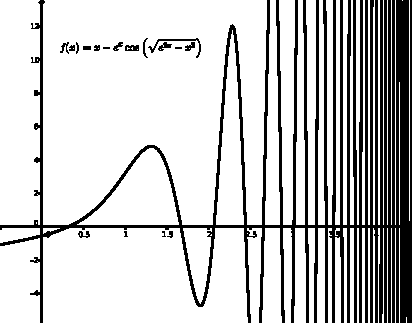
\includegraphics{figures/roots-newton2}
\end{figure}
 \ref{fig:rootFindingExample}. Fungsi ini berosilasi secara liar,
dan osilasinya semakin liar ketika $x$ bertambah. Grafik memotong
sumbu $x$ sebanyak 29 kali pada interval dari $0$ hingga $4.5$
sehingga mempunyai 29 akar di sana! Akar-akarnya adalah
\[
\begin{gathered}.3181315052047641,\ 1.668024051576096,\ 2.062277729598284,\\
2.439940377216816,\ 2.653191974038697,\ldots
\end{gathered}
\]
dan dapat ditemukan dengan metode Newton menggunakan nilai awal $0,1.5,2,2.4,2.6,\ldots$.
Dapatkah Anda menemukan akar berikutnya? Jawaban \vpageref{que:nextRoot}.

\subsection{Metode Sekan (kode semu)\index{metode sekan!kode semu}}

Implementasi langsung metode sekan dapat dengan mudah menjadi tidak
efisien karena banyaknya kemunculan $g$ dalam rumus (\ref{eq:secantMethod}).
Kode semu di bawah ini sangat berhati-hati agar tidak menghitung setiap
nilai $g$ lebih dari sekali. Jika kode itu tampak lebih rumit daripada
yang diperlukan, kemungkinan inilah sumber kerumitannya.

\begin{pseudocode} 
\begin{description}
\item [{Asumsi:}] $g$ mempunyai akar di $\hat{x}$. $g$ terdiferensialkan
dalam suatu lingkungan $\hat{x}$. $x_{0}$ dan $x_{1}$ cukup dekat
dengan $\hat{x}$.
\item [{Masukan:}] Nilai awal $x_{0}$ dan $x_{1}$; fungsi $g$; akurasi
yang diinginkan $tol$; jumlah maksimum iterasi $N$.
\item [{Langkah~1:}] Tetapkan $y_{0}=g(x_{0})$; $y_{1}=g(x_{1})$
\item [{Langkah~2:}] Untuk $j=1\ldots N$ lakukan Langkah 3--5:

\begin{description}
\item [{Langkah~3:}] Tetapkan $x=x_{1}-y_{1}\frac{x_{1}-x_{0}}{y_{1}-y_{0}}$;
\item [{Langkah~4:}] Jika $|x-x_{1}|\leq tol$ maka kembalikan $x$;
\item [{Langkah~5:}] Tetapkan $x_{0}=x_{1}$; $y_{0}=y_{1}$; $x_{1}=x$;
$y_{1}=g(x_{1})$
\end{description}
\item [{Langkah~6:}] Cetak ``Metode gagal. Jumlah maksimum iterasi terlampaui.''
\item [{Keluaran:}] Hampiran $x$ yang mendekati akar eksak, atau pesan
kegagalan.
\end{description}
\end{pseudocode}  

\subsection{Metode Sekan dengan Satu Nilai Awal (kode semu) \index{metode sekan dengan satu nilai awal}\index{metode!sekan dengan satu nilai awal|see{metode sekan dengan satu nilai awal}}\index{metode sekan dengan satu nilai awal!kode semu}}

Kelemahan terbesar metode sekan adalah keharusan adanya dua nilai
awal. Keduanya harus berdekatan, tetapi seberapa dekat, dan bagaimana
Anda menentukannya? Pertanyaan-pertanyaan ini sulit, dan jawaban paling
sederhana sekalipun tetap rumit. Salah satu pendekatan yang masuk
akal ialah menetapkan $x_{1}=x_{0}+g(x_{0})$. Dengan asumsi $x_{0}$
dekat dengan suatu akar, $g(x_{0})$ akan kecil, sehingga $x_{1}$
akan dekat dengan $x_{0}$. Pendekatan ini membebaskan pengguna dari
beban memilih nilai awal kedua. Ada kalanya pemilihan otomatis semacam
itu tidak diinginkan, sehingga metode sekan dengan dua nilai awal
dan metode sekan dengan satu nilai awal sama-sama berguna. Metode
sekan dengan satu nilai awal hanya bekerja dengan baik jika hampiran
awalnya baik.

\begin{pseudocode} 
\begin{description}
\item [{Asumsi:}] $g$ mempunyai akar di $\hat{x}$. $g$ terdiferensialkan
dalam suatu lingkungan $\hat{x}$. $x_{0}$ cukup dekat dengan $\hat{x}$.
\item [{Masukan:}] Nilai awal $x_{0}$; fungsi $g$; akurasi yang diinginkan
$tol$; jumlah maksimum iterasi $N$.
\item [{Langkah~1:}] Tetapkan $y_{0}=g(x_{0})$; $x_{1}=x_{0}+y_{0}$;
$y_{1}=g(x_{1})$
\item [{Langkah~2:}] Untuk $j=1\ldots N$ lakukan Langkah 3--5:

\begin{description}
\item [{Langkah~3:}] Tetapkan $x=x_{1}-y_{1}\frac{x_{1}-x_{0}}{y_{1}-y_{0}}$;
\item [{Langkah~4:}] Jika $|x-x_{1}|\leq tol$ maka kembalikan $x$;
\item [{Langkah~5:}] Tetapkan $x_{0}=x_{1}$; $y_{0}=y_{1}$; $x_{1}=x$;
$y_{1}=g(x_{1})$
\end{description}
\item [{Langkah~6:}] Cetak ``Metode gagal. Jumlah iterasi maksimum terlampaui.''
\item [{Keluaran:}] Hampiran $x$ di dekat akar eksak, atau pesan kegagalan.
\end{description}
\end{pseudocode}  

\subsection{Konsep Utama}
\begin{description}
\item [{Teorema~Akar~Rasional:}] \index{Teorema!Akar Rasional} Jika
polinom $p(x)=a_{0}+a_{1}x+\cdots+a_{k}x^{k}$ memiliki koefisien
rasional, maka setiap akar rasional dari $p$ termasuk dalam himpunan
$\left\{ \frac{n}{d}:n\mbox{ merupakan faktor dari }a_{0}\mbox{ dan }d\mbox{ merupakan faktor dari }a_{k}\right\} $.
\item [{Pembagian~sintetis:}] \index{pembagian!sintetis} Metode untuk
menghitung hasil bagi suatu polinom oleh suatu monomial. Contoh \vpageref{syntheticDivisionExample}.
\item [{Metode~Newton:}] \index{metode Newton} Metode pencarian akar
yang umumnya berkonvergensi ke suatu akar dari $g(x)$ secara kuadratik,
tetapi memerlukan penggunaan turunan. Dalam metode ini, $x_{0}$ dipilih
dan $x_{n+1}=x_{n}-\frac{g(x_{n})}{g'(x_{n})}$ dihitung untuk setiap
$n>1$.
\item [{Metode~sekan:}] \index{metode sekan} Metode pencarian akar yang
umumnya berkonvergensi ke suatu akar dari $g(x)$ dengan orde sekitar
$1.618$, tetapi tidak memerlukan penggunaan turunan. Dalam metode
ini, $x_{0}$ dan $x_{1}$ dipilih dan $x_{n+1}=x_{n}-g(x_{n})\frac{x_{n}-x_{n-1}}{g(x_{n})-g(x_{n-1})}$
dihitung untuk setiap $n>0$.
\item [{Metode~sekan}] dengan satu nilai~awal: \index{metode sekan dengan satu nilai awal}
Modifikasi metode sekan yang memilih $x_{0}$ dan menetapkan $x_{1}=x_{0}+g(x_{0})$.
\end{description}
\startexercises

\subsection{Latihan}
\begin{enumerate}
\item \octave\ \label{enu:newtonsMethodCode}Tulis kode Octave yang mengimplementasikan
metode Newton sebagai sebuah fungsi.
\item \octave\ \label{enu:secantMethodCode}Tulis kode Octave yang mengimplementasikan
metode sekan sebagai sebuah fungsi.
\item \octave\ \label{enu:seededSecantMethodCode}Tulis kode Octave yang
mengimplementasikan metode sekan dengan satu nilai awal sebagai sebuah
fungsi.
\item \octave\ \label{newton-1}Gunakan fungsi metode Newton yang Anda
buat pada soal \ref{enu:newtonsMethodCode} dengan toleransi $10^{-5}$
untuk mencari solusi persamaan

\begin{enumerate}
\item $e^{x}+2^{-x}+2\cos x-6=0$ menggunakan $1\leq x_{0}\leq2$.
\item $\ln(x-1)+\cos(x-1)=0$ menggunakan $1.3\leq x_{0}\leq2$.
\item $2x\cos x-(x-2)^{2}=0$ menggunakan $2\leq x_{0}\leq3$. \hasananswer 
\item $2x\cos x-(x-2)^{2}=0$ menggunakan $3\leq x_{0}\leq4$. \hasananswer 
\item $(x-2)^{2}-\ln x=0$ menggunakan $1\leq x_{0}\leq2$.
\item $(x-2)^{2}-\ln x=0$ menggunakan $e\leq x_{0}\leq4$.
\end{enumerate}
\item \octave\ \label{secant}Ulangi latihan \ref{newton-1} dengan menggunakan
kode metode sekan Anda dari soal \ref{enu:secantMethodCode}. Pilih
nilai $x_{1}$ dari interval yang sama dengan $x_{0}$, tetapi tidak
sama dengan $x_{0}$. \haspartwithanswer 
\item \octave\ \label{exc:newton}Ulangi latihan \ref{secant} dengan menggunakan
kode metode sekan dengan satu nilai awal Anda dari soal \ref{enu:seededSecantMethodCode}. \haspartwithanswer 
\item \octave\ \label{exc:newton-1}Ulangi latihan \ref{secant} dengan
toleransi $10^{-10}$. Dengan menganggap nilai baru ini sebagai nilai
eksak, apakah penggunaan toleransi $10^{-5}$ memberikan hasil dengan
galat terhadap nilai eksak paling besar $10^{-5}$?  \haspartwithanswer 
\item \label{exc:newton-2}Misalkan $g(x)=\frac{100}{x^{2}}\sin\left(\frac{10}{x}\right)$
dan $x_{0}=1.25$. Tentukan $x_{1}$ dan $x_{2}$ yang dihasilkan
oleh metode Newton. \hasasolution 
\item \label{newton1}Misalkan $g(x)=2\ln(1+x^{2})-x$. Tentukan $x_{14}$
menggunakan metode Newton dengan

\begin{enumerate}
\item $x_{0}=5$
\item $x_{0}=1.2$  \hasananswer 
\end{enumerate}
\item Misalkan $g(x)=2\ln(1+x^{2})-x$. Tentukan $x_{2}$ dan $x_{3}$ menggunakan
metode sekan dengan

\begin{enumerate}
\item \label{exc:newton-3}$x_{0}=5$ dan $x_{1}=6$ \hasasolution 
\item $x_{0}=1$ dan $x_{1}=2$
\end{enumerate}
\item Bandingkan metode sekan dan metode Newton berdasarkan hasil pada soal
\ref{secant} dan \ref{newton-1}. Metode mana yang menemukan akar
dengan jumlah iterasi lebih sedikit? Metode mana yang paling jarang
gagal? Metode mana yang lebih baik?
\item Hitung tiga iterasi pertama metode Newton yang diterapkan pada $g(x)=x-(\sqrt{2})^{x}$
dengan $x_{0}=3$.
\item Tentukan nilai $x_{0}$ yang menyebabkan metode Newton gagal konvergen
ke suatu akar $g(x)=2+x-e^{x}$.
\item Jelaskan mengapa metode Newton gagal konvergen untuk fungsi $g(x)=x^{2}+x+1$
dengan $x_{0}=1$.
\item \label{exc:newton-4}Misalkan $h(x)={\displaystyle \frac{2\ln(1+x^{2})-x}{1+x^{2}}}.$
Perhatikan bahwa $h$ dan fungsi $g$ dari soal \ref{newton1} mempunyai
akar yang sama (karena membagi suatu fungsi dengan $1+x^{2}$ tidak
mengubah akar-akarnya). Penggunaan metode Newton untuk mencari akar
$h(x)$ dengan (a) $x_{0}=5$ menghasilkan $x_{14}=8.6624821192$
sedangkan dengan (b) $x_{0}=1.2$ menghasilkan $x_{14}=0$. Bandingkan
nilai-nilai $x_{14}$ tersebut dengan hasil iterasi keempat belas
pada soal \ref{newton1} dan jelaskan setiap persamaan atau perbedaannya. \hasananswer 
\item \label{exc:newton-5}Misalkan $g(x)=e^{3x}-27x^{6}+27x^{4}e^{x}-9x^{2}e^{2x}$
dan $p_{0}=4$. Tentukan $p_{10}$ menggunakan metode Newton. PETUNJUK:
$g'(x)=3e^{3x}-18(x+x^{2})e^{2x}+27(x^{4}+4x^{3})e^{x}-162x^{5}$.
 \hasananswer 
\item Metode Newton tidak menghasilkan solusi semu. Misalkan $f(x)=x-\frac{g(x)}{g'(x)}$
dan $g'(\hat{x})\neq0$. Buktikan bahwa $\hat{x}$ merupakan akar
$g$ jika dan hanya jika $\hat{x}$ merupakan titik tetap $f$. Petunjuk:
salah satu arah pembuktian telah diberikan dalam teks pada bagian
ini.
\item \label{exc:newton-6}Polinom $g(x)=x^{4}+2x^{3}-x-3$ mempunyai akar
$\hat{x}\approx1.097740792$. Tentukan lingkungan terbesar $(a,b)$
dari $\hat{x}$ sedemikian rupa sehingga metode Newton konvergen ke
$\hat{x}$ untuk setiap nilai awal $x_{0}\in(a,b)$.  \hasasolution 
\item \octave\ Gunakan metode Newton untuk menemukan solusi negatif dari
\[
0=12x^{4}-13x^{3}+7x^{2}+x-130
\]
dengan pembulatan ke kelipatan $10^{-4}$ terdekat. Nilai awal apa
yang Anda gunakan? Berapa iterasi yang diperlukan?
\item \label{exc:newton-7}Perhatikan fungsi $g(x)=e^{6x}+3(\ln2)^{2}e^{2x}-(\ln8)e^{4x}-(\ln2)^{3}$.
Hitung iterasi metode Newton secukupnya dengan $x_{0}=0$ untuk menghampiri
sebuah akar $g$ dengan toleransi $0.0002$. Bentuk barisan delta-kuadrat
Aitken $\langle a_{n}\rangle$. Apakah orde kekonvergenannya meningkat? \hasananswer 
\item \label{exc:newton-8}Seperti metode Newton, metode sekan dapat dengan
mudah dijelaskan secara geometris: Tarik garis yang melalui dua titik
$(x_{0},f(x_{0}))$ dan $(x_{1},f(x_{1}))$. Tentukan perpotongan
garis ini dengan sumbu $x$. Koordinat $x$ titik perpotongan tersebut
adalah $x_{2}$. Tentukan $x_{3}$ dengan mencari perpotongan garis
yang melalui $(x_{1},f(x_{1}))$ dan $(x_{2},f(x_{2}))$ dengan sumbu
$x$. Lanjutkan demikian. Gambarkan grafik polinom $p(x)=x^{3}-3x+3$,
dan tunjukkan secara grafis iterasi pertama metode sekan untuk $x_{0}=-1$
dan $x_{1}=-2$.  \hasasolution 
\item Misalkan Anda menggunakan metode sekan dengan $x_{0}=1$ dan $x_{1}=1.1$
untuk mencari akar $f(x)$. 

\begin{enumerate}
\item Tentukan $x_{2}$ jika diketahui $f(1)=0.3$ dan $f(1.1)=0.23$.
\item Buatlah sketsa (grafik) yang menggambarkan perhitungan tersebut. PETUNJUK:
$x_{2}$ terletak di tempat garis yang melalui $(x_{0},f(x_{0}))$
dan $(x_{1},f(x_{1}))$ memotong sumbu $x$.
\end{enumerate}
\item \label{exc:newton-9}Gunakan grafik $g$ untuk menjawab pertanyaan
berikut. $g$ mempunyai akar di $-2\pi,-\pi,\pi,$ dan $2\pi$.  \hasananswer 

\begin{center}
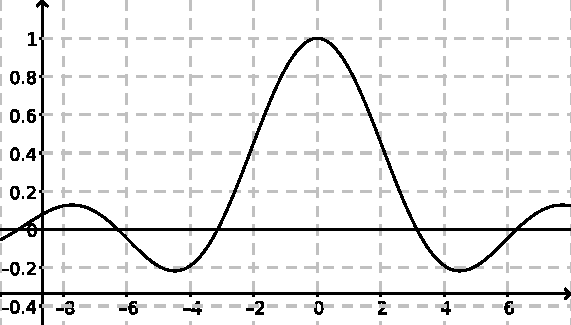
\includegraphics[scale=0.6]{figures/roots-newton4}
\par\end{center}
\begin{enumerate}
\item Metode Newton akan konvergen ke akar yang mana jika $x_{0}=2.5$?
\item Apa yang akan terjadi jika $x_{0}=0$?
\item Tentukan suatu nilai bilangan bulat positif untuk $x_{0}$ yang membuat
metode Newton konvergen ke $2\pi$.
\item Tentukan nilai negatif $x_{0}$, dibulatkan ke persepuluhan terdekat,
yang membuat metode Newton konvergen ke $2\pi$.
\end{enumerate}
\item Gambarkan grafik polinom $p(x)=x^{3}-3x+3$, dan tunjukkan secara
grafis metode Newton untuk $x_{0}=-1$.
\item \octave\ \label{exc:newton-10}Gunakan kode Anda dari soal \ref{enu:secantMethodCode}
untuk mencari sebuah akar fungsi pada interval di soal \ref{enu:bisectionExamples}
\vpageref{enu:bisectionExamples} dengan galat kurang dari $10^{-8}$.
Bandingkan jawaban Anda dengan jawaban dari soal \ref{exc:bisection3}
\vpageref{exc:bisection3}. \hasananswer 
\item \label{exc:newton-11}Jumlah dua bilangan adalah 20. Jika setiap bilangan
dijumlahkan dengan akar kuadratnya, hasil kali kedua jumlah tersebut
adalah $172.2$. Tentukan kedua bilangan itu dengan galat paling besar
$10^{-4}$ dari nilai eksaknya. \hasasolution 
\item \label{exc:newton-12}Berikan contoh situasi ketika metode Newton
gagal pada iterasi kedua (yaitu, $x_{1}$ dapat dihitung tetapi $x_{2}$
tidak dapat dihitung). \hasasolution 
\item Misalkan $h(x)=2.2x^{3}-6.6x^{2}+4.4x$ dan $g(x)=h^{\circ3}(x)$.
Artinya, $g(x)=h(h(h(x)))$. Hampiri salah satu akar $g'(x)$.
\item \label{graph}Untuk nilai-nilai $x_{0}$ mana, secara hampiran, metode
Newton akan konvergen ke $-2.5$?

\begin{center}
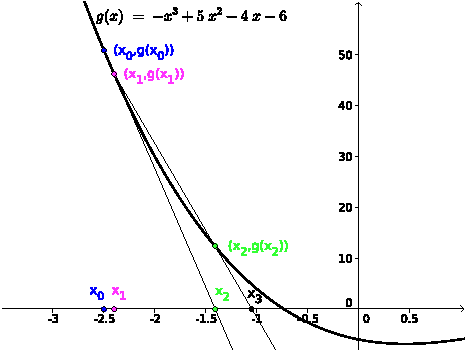
\includegraphics[width=5.5cm]{figures/roots-newton3}
\par\end{center}
\item Untuk fungsi yang ditampilkan pada soal \ref{graph}, tentukan $x_{2}$
dan $x_{3}$ pada metode sekan dengan $x_{0}=-10$ dan $x_{1}=6$.
\item \label{exc:newton-13}Misalkan 
\[
f(x)=10-\int_{0}^{x}\frac{e^{t}}{1+t}\,dt.
\]
Hampiri akar positif $f$. \hasananswer 
\item Dari metode pencarian akar yang telah kita bahas sejauh ini (metode
bagi dua, iterasi titik tetap, metode Newton, metode sekan, dan metode
Steffensen), metode mana yang menurut Anda paling baik? Mengapa?
\end{enumerate}
\noindent\finishexercises

\subsection*{Jawaban}
\begin{description}
\item [{Kekonvergenan~kuadratik?}] \label{que:quadraticConvergence}$\ $

\begin{center}
\begin{tabular}{c|ccc}
$n$ & $x_{n}$ & $\quad$ & $x_{n}$\tabularnewline
\hline 
0 & $2$ &  & $-1$\tabularnewline
1 & $2.5$ &  & $-.7647058823529411$\tabularnewline
2 & $2.666666666666667$ &  & $-.7326286052763475$\tabularnewline
3 & $2.722222222222227$ &  & $-.7320509933083684$\tabularnewline
4 & $2.731741086881274$ &  & $-.7320508075688965$\tabularnewline
5 & $2.732050478023325$ &  & \tabularnewline
6 & $2.732050807568503$ &  & \tabularnewline
$\vdots$ & $\vdots$ &  & $\vdots$\tabularnewline
 & $2.732050807568877$ &  & $-.7320508075688772$\tabularnewline
\end{tabular}
\par\end{center}

Kekonvergenannya tampak kuadratik karena jumlah angka signifikan yang
akurat kurang lebih berlipat dua selama beberapa iterasi terakhir.
\item [{Metode~sekan~secara}] geometris? \label{que:secantMethodGeometrically}
Bandingkan representasi geometris metode sekan berikut dengan representasi
metode Newton (pada halaman \pageref{img:newtonsMethod}). Pada metode
Newton, perpotongan garis singgung dengan sumbu $x$ menentukan iterasi
berikutnya. Pada metode sekan, perpotongan garis sekan dengan sumbu
$x$ menentukan iterasi berikutnya.
\begin{center}
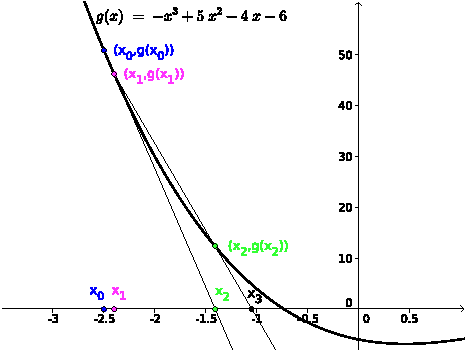
\includegraphics{figures/roots-newton3}
\par\end{center}
\item [{Akar~berikutnya?}] \label{que:nextRoot} Akar berikutnya kira-kira
$2.872257717171606$. Akar ini dapat ditemukan, misalnya, dengan metode
Newton menggunakan $x_{0}=2.81$. Perhatikan bahwa perhitungan ini
sangat peka terhadap kondisi awal karena terdapat begitu banyak akar
yang saling berdekatan. Sebagai contoh, memulai dengan $x_{0}=2.8$
justru menghasilkan akar $9.662623060421268$!
\end{description}




\section{\label{sec:moreConvergenceDiagrams}Diagram Kekonvergenan Lainnya}

Fungsi kubik $g(x)=1-x^{3}$ memiliki satu akar riil, $1$. Namun,
fungsi tersebut juga memiliki dua akar kompleks. Jika Anda telah mempelajari
analisis kompleks, Anda mungkin sudah mengetahui kedua akar lainnya.
Bahkan jika belum, Anda dapat menentukannya dengan teknik dasar prakalkulus.
Karena $1$ merupakan akar, Anda dapat menggunakan pembagian sintetis
untuk melakukan deflasi pada polinom:

\begin{center}
\begin{tabular}{ccccc}
\multicolumn{1}{c|}{$1$} & $-1$ & $0$ & $0$ & $1$\tabularnewline
\cline{1-1}
 &  & $-1$ & $-1$ & $-1$\tabularnewline
\hline 
 & $-1$ & $-1$ & \multicolumn{1}{c|}{$-1$} & \multicolumn{1}{c|}{$0$}\tabularnewline
\cline{5-5}
\end{tabular}
\par\end{center}

\noindent Pembagian ini menunjukkan bahwa $g(x)=(x-1)(-x^{2}-x-1)$,
sehingga kedua akar lainnya merupakan solusi persamaan $-x^{2}-x-1=0$;
dengan demikian, persoalannya tereduksi menjadi persamaan kuadrat.
Solusinya adalah $\frac{1\pm\sqrt{1-4}}{-2}=-\frac{1}{2}\pm i\frac{\sqrt{3}}{2}$.
Selain itu, Anda mungkin mengenali $1-x^{3}$ sebagai salah satu bentuk
khusus polinom, yakni selisih dua kubus. 

Tentu saja semua ini menarik, tetapi apa hubungannya dengan analisis
numerik? Mungkin mengejutkan bahwa iterasi titik tetap (dan karena
itu metode Newton), metode sekan, serta metode Steffensen dapat digunakan
untuk menemukan akar kompleks sama baiknya dengan akar riil! Bahkan
algoritmenya tidak perlu dimodifikasi! Namun, bahasa pemrograman yang
digunakan untuk menerapkan metode-metode tersebut harus mampu menangani
aritmetika bilangan kompleks. Octave mendukungnya secara langsung.

Pertama, mencari akar $g(x)=1-x^{3}$ setara dengan mencari titik
tetap $f(x)=1/x^{2}$. Mengapa? Lihat jawabannya \vpageref{que:whyEquivalent}.
Dengan menetapkan $x_{0}=-1+i$ lalu menerapkan metode Newton dan
metode sekan pada $g(x)=1-x^{3}$, serta metode Steffensen pada $f(x)=1/x^{2}$
kita memperoleh hasil berikut:

\begin{center}
\begin{tabular}{c|ccc}
 & \multicolumn{3}{c}{$x_{i}$}\tabularnewline
\cline{2-4}
$i$ & Steffensen & Sekan & Newton\tabularnewline
\hline 
$0$ & $-1+i$ & $-1+i$ & $-1+i$\tabularnewline
$1$ & $-0.85+0.8i$ & $-0.66666666+0.83333333i$ & $-0.66666666+0.83333333i$\tabularnewline
$2$ & $-0.60313824+0.67770639i$ & $-0.55034016+0.82376444i$ & $-0.50869191+0.84109987i$\tabularnewline
$3$ & $-0.39846066+0.84671567i$ & $-0.49763752+0.85554014i$ & $-0.49932999+0.86626917i$\tabularnewline
$4$ & $-0.51660491+0.84998590i$ & $-0.49932718+0.86627140i$ & $-0.49999991+0.86602490i$\tabularnewline
$5$ & $-0.49910537+0.86543351i$ & $-0.50000774+0.86602504i$ & $-0.50000000+0.86602540i$\tabularnewline
$6$ & $-0.50000228+0.86602568i$ & $-0.49999999+0.86602540i$ & \tabularnewline
$7$ & $-0.50000000+0.86602540i$ & $-0.50000000+0.86602540i$ & \tabularnewline
$8$ & $\vdots$ & $\vdots$ & $\vdots$\tabularnewline
\end{tabular}
\par\end{center}

\noindent Setiap barisan dengan cepat konvergen ke akar kompleks $-\frac{1}{2}+\frac{\sqrt{3}}{2}i$.
Ini bukan kebetulan ataupun contoh yang dibuat-buat. Secara umum,
metode-metode ini bekerja sama baiknya di bidang kompleks maupun pada
garis riil. Kita pun dapat menemukan akar riil dengan memulai dari
bilangan kompleks. Sebagai contoh, jika nilai awal $x_{0}$ diubah
menjadi $1+i$, metode Newton konvergen ke $1$.

Setelah memperluas cakupan metode-metode ini ke bilangan kompleks,
kini ada jenis diagram kekonvergenan baru yang perlu dipertimbangkan.
Kita dapat mengamati pola kekonvergenan ketiga metode untuk banyak
nilai awal di bidang kompleks, bukan hanya pada garis riil. Gambar
\ref{fig:complexConvergenceDiagram1} menampilkan diagram kekonvergenan
metode Newton dengan $g(x)=1-x^{3}$, metode sekan dengan satu nilai
awal untuk $g(x)=1-x^{3}$, dan metode Steffensen dengan $f(x)=1/x^{2}$.
\begin{figure}
\caption{\label{fig:complexConvergenceDiagram1}Diagram kekonvergenan pada
bidang kompleks.}

\begin{centering}
\begin{tabular}{cc}
\multirow{3}{5cm}{\textbf{Urutan dari atas ke bawah:}\\
metode Newton dengan
\[
g(x)=1-x^{3}
\]
dan dwell 20;\\
metode sekan dengan satu nilai awal untuk
\[
g(x)=1-x^{3}
\]
dan dwell 40;\\
metode Steffensen dengan
\[
f(x)=\frac{1}{x^{2}}
\]
dan dwell 40.\\
Setiap diagram mencakup bagian bidang kompleks dengan bagian riil
dalam $[-5,5]$ dan bagian imajiner dalam $[-3.75,3.75]$.} & \includegraphics[scale=0.4]{figures/convergenceDiagram1\lyxdot 1}\tabularnewline
 & \includegraphics[scale=0.4]{figures/convergenceDiagram1\lyxdot 2a}\tabularnewline
 & \includegraphics[scale=0.4]{figures/convergenceDiagram1\lyxdot 3}\tabularnewline
\end{tabular}
\par\end{centering}
\end{figure}
Setiap diagram mencakup bagian bidang kompleks dengan bagian riil
dalam $[-5,5]$ dan bagian imajiner dalam $[-3.75,3.75]$. Sudut kiri
atas setiap diagram mewakili nilai awal $-5+3.75i$ sedangkan sudut
kanan bawah mewakili nilai awal $5-3.75i$. Pusat setiap diagram mewakili
nilai awal $0$. Warna-warna tersebut bersesuaian dengan ketiga akar:
merah dengan $1$, hijau dengan $-\frac{1}{2}+\frac{\sqrt{3}}{2}i$,
dan biru dengan $-\frac{1}{2}-\frac{\sqrt{3}}{2}i$. Hitam menandakan
kegagalan mencapai kekonvergenan. Perbedaan intensitas warna merah,
hijau, dan biru menunjukkan jumlah iterasi yang diperlukan metode
untuk konvergen. Semakin tinggi intensitas, semakin sedikit iterasinya.
Untuk $x_{0}=5-3.75i$, terlihat bahwa metode Newton dan metode sekan
dengan satu nilai awal sama-sama konvergen ke $-\frac{1}{2}+\frac{\sqrt{3}}{2}i$,
karena sudut kanan atas setiap diagram berwarna hijau. Sebaliknya,
metode Steffensen gagal konvergen ke akar mana pun jika dimulai dari
$x_{0}=5-3.75i$, sebagaimana ditunjukkan oleh warna hitam di sudut
kanan atas diagram kekonvergenan.

Dwell menyatakan jumlah maksimum iterasi yang diperbolehkan. Jadi,
titik-titik hitam sebenarnya mewakili nilai awal yang belum mencapai
kekonvergenan dalam jumlah iterasi yang tidak melebihi dwell. Ini
berbeda dengan menyatakan bahwa metode tersebut sama sekali tidak
konvergen untuk nilai-nilai awal itu. Sebagian nilai awal yang ditampilkan
hitam mungkin tetap menghasilkan kekonvergenan jika diberi lebih banyak
iterasi.

Ada dua hal yang sangat mencolok pada diagram kekonvergenan ini. Pertama,
metode sekan dengan satu nilai awal dan metode Newton konvergen untuk
himpunan nilai awal yang jauh lebih besar daripada metode Steffensen.
Hal ini, setidaknya sebagian, disebabkan oleh fungsi yang dipilih.
Untuk fungsi lain, mungkin ada skema titik tetap yang membuat metode
Steffensen konvergen pada himpunan nilai awal yang besar pula. Kedua,
pola warnanya sangat rumit, bahkan bersifat fraktal. Memprediksi akar
mana yang akan dicapai suatu metode untuk nilai awal tertentu---dan
bahkan apakah metode itu akan konvergen sama sekali---merupakan persoalan
yang sangat sulit! Padahal analisis ini dilakukan pada fungsi yang
cukup sederhana.

Sekarang pertimbangkan persoalan yang jauh lebih rumit---mencari
akar $g(z)=e^{z}-z$ atau, secara ekuivalen, mencari titik tetap $f(z)=e^{z}$.
Grafik $f(z)$ pada bilangan riil akan segera meyakinkan Anda bahwa
tidak ada solusi riil. Diperlukan pemikiran lebih lanjut untuk menentukan
sifat solusi kompleksnya.

Untuk itu, tetapkan bilangan riil $a_{0}$ dan tinjau garis vertikal
di bidang kompleks, $L_{a_{0}}=\{a_{0}+ib:b\in\mathbb{R}\}$. Citra
$L_{a_{0}}$ oleh fungsi eksponensial adalah sebuah lingkaran berjari-jari
$e^{a_{0}}$ yang berpusat di titik asal. Memang, $e^{a_{0}+ib}=e^{a_{0}}e^{ib}=e^{a_{0}}(\cos b+i\sin b)$.
Jadi, $b$ memparameterkan lingkaran yang berpusat di titik asal dengan
jari-jari $e^{a_{0}}$. Sekarang, misalkan $L_{a_{0}}$ memuat sebuah
titik tetap, $\hat{z}=a_{0}+i\hat{b}$, dari fungsi eksponensial,
$f(z)=e^{z}$. Maka $\hat{z}=f(\hat{z})$, atau $a_{0}+i\hat{b}=e^{a_{0}}(\cos\hat{b}+i\sin\hat{b})$.
Kita menyimpulkan bahwa garis dan lingkaran tersebut berpotongan di
titik tetap itu. Setiap titik tetap $f$ niscaya merupakan titik potong
antara garis $L_{a_{0}}$ dan lingkaran $C_{a_{0}}$ untuk suatu $a_{0}$.
Gambar 
\begin{figure}
\caption{\label{fig:verticalLineAndCircle}Sebuah garis vertikal dan citranya
oleh fungsi eksponensial.}

\centering{}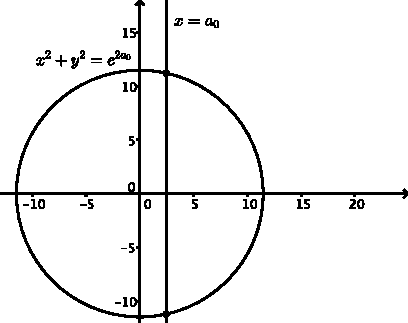
\includegraphics{figures/roots-more2}
\end{figure}
\ref{fig:verticalLineAndCircle} memperlihatkan contoh yang mewakili.
Faktanya, diagram tersebut memperlihatkan kasus yang menarik: $x=a_{0}\approx2.439940377216816$.
Koordinat kedua titik potong adalah 
\[
(2.439940377216816,\pm11.2098911414971).
\]
Hal menariknya ialah 
\[
e^{2.439940377216816+11.2098911414971i}\approx2.439940377216816-11.2098911414971i
\]
dan 
\[
e^{2.439940377216816-11.2098911414971i}\approx2.439940377216816+11.2098911414971i.
\]
Kedua titik tersebut saling menjadi citra satu sama lain oleh fungsi
eksponensial! Titik-titik yang kita temukan di sini disebut titik
periodik. Jika kita tetapkan $z_{1}=2.439940377216816-11.2098911414971i$
dan $z_{2}=2.439940377216816+11.2098911414971i$, maka $e^{z_{1}}=z_{2}$
dan $e^{z_{2}}=z1$. Oleh karena itu, jika kita melakukan iterasi
$z_{2}=f(z_{1})$, $z_{3}=f(z_{2})$, $z_{4}=f(z_{3})$, $z_{5}=f(z_{4})$,
dan seterusnya, barisan $z_{1},z_{2},z_{3},z_{4},\ldots$ sebenarnya
berbentuk
\[
z_{1},z_{2},z_{1},z_{2},z_{1},z_{2},\ldots.
\]
Barisan itu hanya bolak-balik antara $z_{1}$ dan $z_{2}$ secara
periodik. Nilai-nilai seperti ini kita sebut titik berperiode 2. Nilai-nilai
tersebut bukan titik tetap $f(z)$ tetapi merupakan titik tetap $f(f(z))$! 

\begin{digression}{Titik periodik.}

\noindent Jika suatu barisan $\langle p_{n}\rangle$ berbentuk
\[
p_{1},p_{2},\ldots,p_{k},p_{1},p_{2},\ldots,p_{k},p_{1},\ldots,\qquad k>1
\]
maka $p_{1}$ disebut titik berperiode $k$ (demikian pula $p_{2},p_{3},\ldots,p_{k}$!). 

\end{digression}

Sebaliknya, $\hat{z}=2.062277729598284+7.588631178472513i$ merupakan
titik tetap (secara hampiran) dari $f(z)$ karena
\[
e^{2.062277729598284+7.588631178472513i}=2.062277729598284+7.588631178472513i.
\]
Selain itu, konjugat $\hat{z}$, yaitu $\overline{\hat{z}}=2.0622377729598284-7.588631178472513i$
juga merupakan titik tetap. Periksalah dengan kalkulator atau Octave!

Secara umum, jika $\hat{z}$ merupakan titik tetap dari $e^{z}$ maka
$\overline{\hat{z}}$ juga merupakan titik tetap:
\[
\hat{z}=e^{\hat{z}}\implies\overline{\hat{z}}=\overline{e^{\hat{z}}}=e^{\overline{\hat{z}}}.
\]
Jadi, ketika kita menemukan satu titik tetap, sebenarnya kita menemukan
dua: titik tetap tersebut dan konjugatnya. 

Kita kini siap kembali meninjau titik-titik potong $L_{a_{0}}$ dan
$C_{a_{0}}$. Anggap $a_{0}+ib$ merupakan titik tetap dari $e^{z}$.
Maka $a_{0}+ib=e^{a_{0}+ib}=e^{a_{0}}(\cos b+i\sin b$), sehingga
\begin{eqnarray}
a_{0} & = & e^{a_{0}}\cos b\nonumber \\
b & = & e^{a_{0}}\sin b\label{eq:expFixedPoint}
\end{eqnarray}
\begin{figure}
\caption{\label{fig:complexConvergenceDiagram2}Diagram kekonvergenan lainnya
pada bidang kompleks.}

\begin{centering}
\includegraphics[scale=0.4]{figures/convergenceDiagram2\lyxdot 1}
\includegraphics[scale=0.4]{figures/convergenceDiagram2\lyxdot 2}
\includegraphics[scale=0.4]{figures/convergenceDiagram2\lyxdot 3} 
\par\end{centering}
\textbf{Urutan dari kiri ke kanan:} metode Newton dengan $g(z)=z-e^{z}$
dan dwell 20; metode sekan dengan $g(z)=z-e^{z}$ dan dwell 40; metode
Steffensen dengan $f(z)=e^{z}$ dan dwell 40. Setiap diagram mencakup
bagian bidang kompleks dengan bagian riil dalam $[-10,30]$ dan bagian
imajiner dalam $[0,73]$.
\end{figure}
Sekarang, karena $a_{0}+ib$ merupakan titik potong, titik itu terletak
pada $C_{a_{0}}$, sehingga $a_{0}^{2}+b^{2}=e^{2a_{0}}\Rightarrow b=\pm\sqrt{e^{2a_{0}}-a_{0}^{2}}$.
Terakhir, dengan menyubstitusikan $b=\sqrt{e^{2a_{0}}-a_{0}^{2}}$
ke \ref{eq:expFixedPoint}, kita memperoleh bahwa suatu titik potong
merupakan titik tetap jika dan hanya jika
\begin{eqnarray}
a_{0} & = & e^{a_{0}}\cos\sqrt{e^{2a_{0}}-a_{0}^{2}}\nonumber \\
 &  & \mbox{dan}\nonumber \\
\sqrt{e^{2a_{0}}-a_{0}^{2}} & = & e^{a_{0}}\sin\sqrt{e^{2a_{0}}-a_{0}^{2}}.\label{eq:realPartRequirement}
\end{eqnarray}
Luangkan waktu untuk memikirkan mengapa  $b=-\sqrt{e^{2a_{0}}-a_{0}^{2}}$
tidak perlu disubstitusikan ke \ref{eq:expFixedPoint}. Petunjuk:
lakukan substitusi dan sederhanakan. Anda akan mendapati bahwa kedua
persamaan yang diperoleh ekuivalen dengan persamaan-persamaan dalam
\ref{eq:expFixedPoint}.

Sebagai contoh, $2.439940377216816-11.2098911414971i$ dan $2.062277729598284+7.588631178472513i$
sama-sama memenuhi persamaan pertama dalam \ref{eq:realPartRequirement},
tetapi $2.439940377216816-11.2098911414971i$ tidak memenuhi persamaan
kedua, sedangkan $2.062277729598284+7.588631178472513i$ memenuhinya.
Jadi, seperti diamati sebelumnya, $2.439940377216816-11.2098911414971i$
bukan titik tetap, tetapi $2.062277729598284+7.588631178472513i$
adalah titik tetap. 

Apakah Anda mengenali persamaan pertama dalam \ref{eq:realPartRequirement}?
Kita pertama kali melihatnya \vpageref{interestingNewton} pada Bagian
\ref{sec:newtonsMethod}. Seperti dicatat di sana, lima solusi terkecil
adalah
\[
\begin{gathered}.3181315052047641,\ 1.668024051576096,\ 2.062277729598284,\\
2.439940377216816,\ 2.653191974038697,\ldots
\end{gathered}
\]
Nilai $2.062277729598284$ dan $2.439940377216816$ menjadi contoh
dalam pembahasan ini. Bagaimana dengan tiga nilai lainnya dalam daftar
tersebut? Apakah nilai-nilai itu menghasilkan titik tetap fungsi eksponensial?
Titik berperiode dua? Atau sesuatu yang lain? Luangkan waktu untuk
menyelidikinya. Jawabannya \vpageref{que:natureOfRoots}. Penyelidikan
dengan Octave terhadap $2.062277729598284$, yang kita ketahui merupakan
titik tetap: \begin{verbatim}
octave:1> format('long')
octave:2> a0=2.062277729598284
a0 =  2.06227772959828
octave:3> b=sqrt(exp(2*a0)-a0^2)
b =  7.58863117847251
octave:4> exp(a0+I*b)
ans =  2.06227772959828 + 7.58863117847251i
\end{verbatim} memverifikasi bahwa $e^{a_{0}+ib}=a_{0}+ib$ untuk $a_{0}=2.062277729598284$,
setidaknya hingga presisi mesin. Nilai eksak titik tetap tersebut
tidak diketahui, tetapi memang demikianlah sifat analisis numerik.

Gambar \ref{fig:complexConvergenceDiagram2} menunjukkan kekonvergenan
menuju 12 titik tetap dari $e^{z}$, masing-masing ditunjukkan oleh
satu dari 12 warna yang berbeda. Koordinat setiap titik tetap dapat
dihampiri dengan mencari titik berintensitas paling tinggi di dalam
setiap pita berwarna. 

Seperti pada Gambar \ref{fig:complexConvergenceDiagram2}, diagram
kekonvergenan untuk metode sekan dapat dibuat dengan menetapkan $x_{1}=x_{0}+\delta$
untuk suatu bilangan kecil $\delta.$ Tidak menjadi masalah apakah
$\delta$ riil atau kompleks. Pemilihan $x_{1}$ secara otomatis dengan
cara ini memungkinkan diagram menunjukkan kekonvergenan atau kedivergenan
hanya berdasarkan $x_{0}$ saja, seperti pada diagram kekonvergenan
lainnya. Anda akan melihat bahwa diagram kekonvergenan metode sekan
dan metode Newton cukup mirip. Secara umum, untuk $\delta$ yang cukup
kecil, hal ini akan berlaku. Diagram kekonvergenan metode sekan dan
metode Newton untuk fungsi yang sama pada wilayah yang sama akan tampak
sangat serupa. Satu-satunya perbedaan penting adalah jumlah iterasi
yang diperlukan untuk konvergen. Metode sekan memerlukan lebih banyak
iterasi.

\noindent\begin{small} 

\subsection{Latihan}
\begin{enumerate}
\item \label{exc:more}Cocokkan setiap fungsi dengan diagram kekonvergenan
metode Newton yang sesuai. Sumbu riil melintasi pusat setiap diagram,
sedangkan sumbu imajiner ditampilkan tetapi tidak selalu berada tepat
di tengah. \hasasolution  
\begin{eqnarray*}
f(x) & = & 56-152x+140x^{2}-17x^{3}-48x^{4}+9x^{5}\\
g(x) & = & (x^{2})(\ln x)+(x-3)e^{x}\\
h(x) & = & 1+2x+3x^{2}+4x^{3}+5x^{4}+6x^{5}\\
l(x) & = & (\ln x)(x^{3}+1)
\end{eqnarray*}

\begin{center}
\begin{tabular}{cccc}
(a) &  & (b) & \tabularnewline
 & 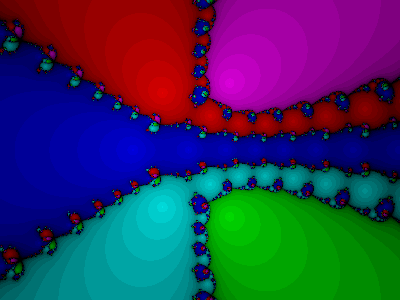
\includegraphics[scale=0.4]{figures/roots-more5} &  & 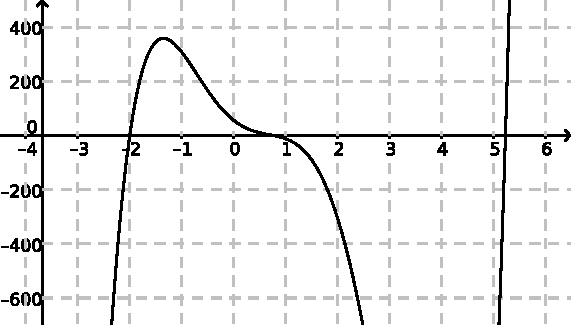
\includegraphics[scale=0.4]{figures/roots-more3}\tabularnewline
(c) &  & (d) & \tabularnewline
 & 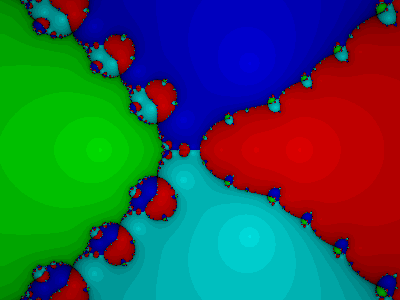
\includegraphics[scale=0.4]{figures/roots-more6} &  & 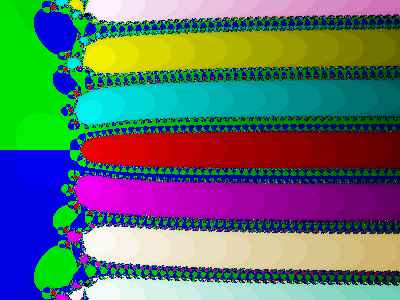
\includegraphics[scale=0.4]{figures/roots-more4}\tabularnewline
\end{tabular}
\par\end{center}
\item \label{exc:more-1}Cocokkan setiap fungsi dengan diagram kekonvergenan
metode Newton yang sesuai. Sumbu riil melintasi pusat setiap diagram,
sedangkan sumbu imajiner ditampilkan tetapi tidak selalu berada tepat
di tengah.  \hasananswer 
\begin{eqnarray*}
f(x) & = & \sin x\\
g(x) & = & \sin x-e^{-x}\\
h(x) & = & e^{x}+2^{-x}+2\cos x-6\\
l(x) & = & x^{4}+2x^{2}+4
\end{eqnarray*}

\begin{center}
\begin{tabular}{cccc}
(a) &  & (b) & \tabularnewline
 & 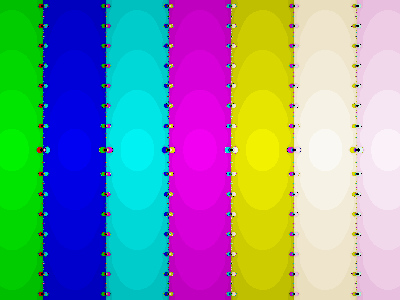
\includegraphics[scale=0.4]{figures/roots-more12} &  & 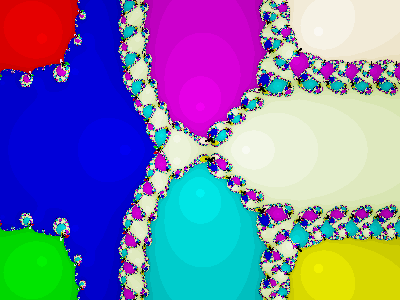
\includegraphics[scale=0.4]{figures/roots-more14}\tabularnewline
(c) &  & (d) & \tabularnewline
 & 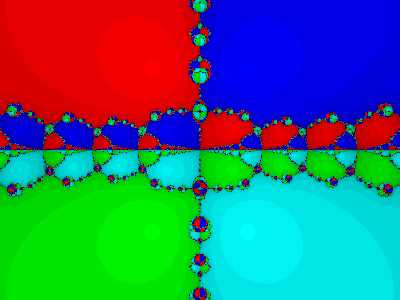
\includegraphics[scale=0.4]{figures/roots-more11} &  & 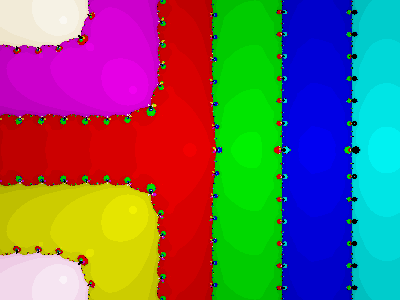
\includegraphics[scale=0.4]{figures/roots-more13}\tabularnewline
\end{tabular}
\par\end{center}
\item \label{polynomials}Tentukan sebuah polinom yang memiliki akar-akar
berikut dan tidak memiliki akar lainnya.

\begin{enumerate}
\item $-7,2,1\pm5i$
\item $-7,2,1+5i$
\item \label{exc:more-2}$-4,-1,2,\pm2i$  \hasasolution 
\item \label{exc:more-4}$-4,-1,2,2i$  \hasasolution 
\item $0,-1\pm i,1\pm i$
\item $-3+i,-2-i,-3i,1-2i$
\end{enumerate}
\item \label{newton}Buat diagram kekonvergenan metode Newton untuk polinom-polinom
pada soal \ref{polynomials}. Pastikan Anda mencakup daerah yang memperlihatkan
setidaknya area kecil yang berkonvergensi ke setiap akar. Kode Octave
dapat diunduh dari \href{http://lqbrin.github.io/tea-time-numerical/ancillaries.html}{situs pendamping}.
\item \label{noroot}Fungsi $f(x)=e^{x}$ dan $g(x)=\frac{1}{x^{2}+1}$
tidak memiliki akar, baik riil maupun kompleks. Temukan setidaknya
dua fungsi lain yang juga tidak memiliki akar.
\item \label{failure}Misalkan $f(x)=\frac{x^{2}-7x+10}{2}+\sin(3x)$.

\begin{enumerate}
\item Temukan semua akar riil dari $f$. Fungsi ini bukan polinom, sehingga
deflasi tidak dapat digunakan. Sebagai gantinya, buatlah grafik fungsi
tersebut dan gunakan metode Newton untuk menemukan akar-akarnya hingga
ketelitian $10^{-8}$. Ada empat akar. 
\item Buat diagram kekonvergenan metode Newton untuk $f$ guna melihat apakah
terdapat akar kompleks. Jika ada, gunakan metode Newton untuk menghampirinya.
Gunakan diagram kekonvergenan tersebut untuk membantu Anda memilih
nilai awal.
\item Dapatkah Anda menemukan semua akar dari $f$?
\end{enumerate}
\item \label{exc:more-3}Cocokkan setiap fungsi dengan diagram kekonvergenan
metode sekan dengan satu nilai awal yang sesuai. Sumbu riil melewati
pusat setiap diagram, sedangkan sumbu imajiner ditampilkan, tetapi
tidak selalu berada di tengah. \hasasolution  
\begin{eqnarray*}
f(x) & = & \sin x\\
g(x) & = & \sin x-e^{-x}\\
h(x) & = & e^{x}+2^{-x}+2\cos x-6\\
l(x) & = & 56-152x+140x^{2}-17x^{3}-48x^{4}+9x^{5}
\end{eqnarray*}

\begin{center}
\begin{tabular}{cccc}
(a) &  & (b) & \tabularnewline
 & 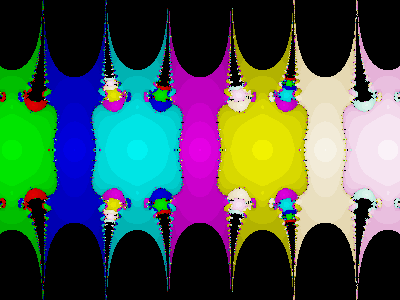
\includegraphics[scale=0.4]{figures/roots-more8} &  & 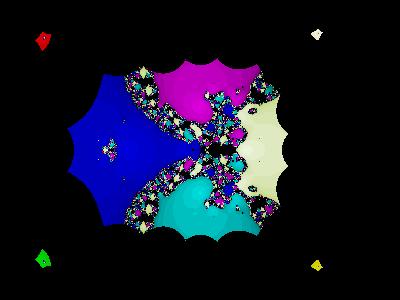
\includegraphics[scale=0.4]{figures/roots-more9}\tabularnewline
(c) &  & (d) & \tabularnewline
 & 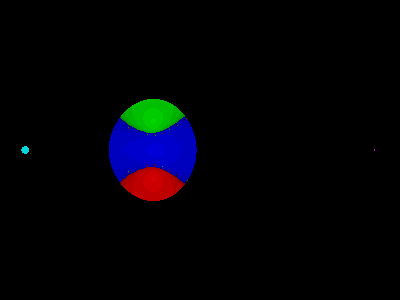
\includegraphics[scale=0.4]{figures/roots-more10} &  & 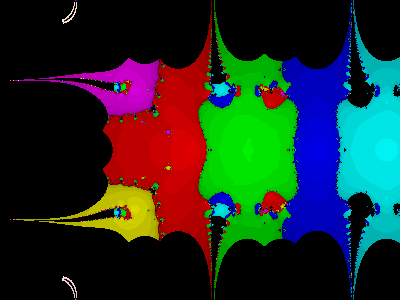
\includegraphics[scale=0.4]{figures/roots-more7}\tabularnewline
\end{tabular}
\par\end{center}
\item \label{exc:more-5}Cocokkan setiap fungsi dengan diagram kekonvergenan
metode sekan dengan satu nilai awal yang sesuai. Sumbu riil melewati
pusat setiap diagram, sedangkan sumbu imajiner ditampilkan, tetapi
tidak selalu berada di tengah. \hasananswer 
\begin{eqnarray*}
f(x) & = & x^{4}+2x^{2}+4\\
g(x) & = & (x^{2})(\ln x)+(x-3)e^{x}\\
h(x) & = & 1+2x+3x^{2}+4x^{3}+5x^{4}+6x^{5}\\
l(x) & = & (\ln x)(x^{3}+1)
\end{eqnarray*}

\begin{center}
\begin{tabular}{cccc}
(a) &  & (b) & \tabularnewline
 & 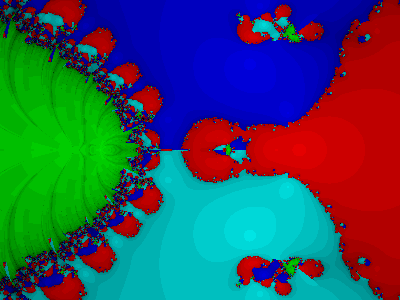
\includegraphics[scale=0.4]{figures/roots-more17} &  & 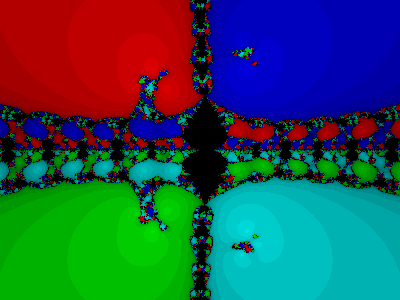
\includegraphics[scale=0.4]{figures/roots-more18}\tabularnewline
(c) &  & (d) & \tabularnewline
 & 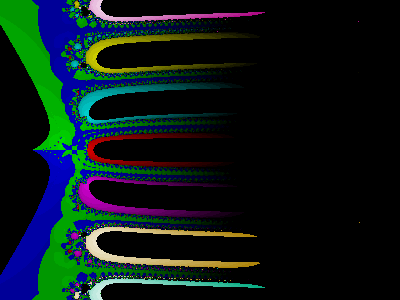
\includegraphics[scale=0.4]{figures/roots-more15} &  & 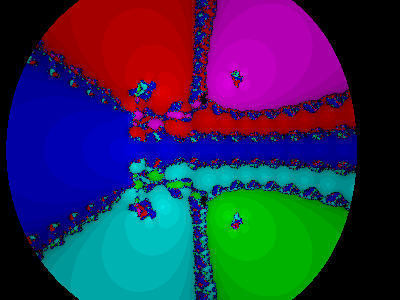
\includegraphics[scale=0.4]{figures/roots-more16}\tabularnewline
\end{tabular}
\par\end{center}
\item Buat diagram kekonvergenan metode sekan dengan satu nilai awal untuk
polinom-polinom pada soal \ref{polynomials}. Pastikan Anda mencakup
daerah yang memperlihatkan setidaknya area kecil yang berkonvergensi
ke setiap akar. Kode Octave dapat diunduh dari \href{http://lqbrin.github.io/tea-time-numerical/ancillaries.html}{situs pendamping}.
\item Diagram kekonvergenan metode Newton untuk suatu polinom sangat mirip
dengan diagram kekonvergenan metode Newton untuk polinom lainnya.
Perubahan menarik pada diagram kekonvergenan metode Newton dan diagram
kekonvergenan metode sekan dengan satu nilai awal dapat diperoleh
dengan mengalikan sebuah polinom dengan fungsi nonpolinom yang tidak
memiliki akar. Buat diagram kekonvergenan metode Newton dan diagram
kekonvergenan metode sekan dengan satu nilai awal untuk hasil kali
fungsi-fungsi pada soal \ref{polynomials} dengan fungsi-fungsi pada
soal \ref{noroot}.
\item Bahas perbandingan keunggulan dan kelemahan metode Newton, metode
sekan, dan metode sekan dengan satu nilai awal.
\end{enumerate}
\end{small}

\subsection*{Jawaban}
\begin{description}
\item [{Mengapa~ekuivalen?}] \label{que:whyEquivalent}Persamaan $g(x)=0$
dan $f(x)=x$ memiliki himpunan penyelesaian yang sama persis. $g(x)=0\Leftrightarrow1-x^{3}=0\Leftrightarrow1=x^{3}\Leftrightarrow\frac{1}{x^{2}}=x\Leftrightarrow f(x)=x$.
\item [{Bagaimana~sifat~akar-akarnya?}] \label{que:natureOfRoots} $.3181315052047641$
merupakan titik tetap dari fungsi eksponensial: \begin{verbatim}
octave:1> format('long')
octave:2> a0=.3181315052047641;
octave:3> b=sqrt(exp(2*a0)-a0^2)
b =  1.33723570143069
octave:4> exp(a0+I*b)
ans =  0.318131505204764 + 1.337235701430689i
\end{verbatim} $1.668024051576096$ merupakan titik berperiode dua dari fungsi eksponensial:
\begin{verbatim}
octave:1> format('long')
octave:2> a0=1.668024051576096;
octave:3> b=sqrt(exp(2*a0)-a0^2)
b =  5.03244706448616
octave:4> exp(a0+I*b)
ans =  1.66802405157609 - 5.03244706448616i
\end{verbatim} $2.653191974038697$ merupakan titik tetap dari fungsi eksponensial:
\begin{verbatim}
octave:5> a0=2.653191974038697;
octave:6> b=sqrt(exp(2*a0)-a0^2)
b =  13.9492083345332
octave:7> exp(a0+I*b)
ans =   2.65319197403878 + 13.94920833453319i 
\end{verbatim}
\end{description}




\section{\label{sec:RootsOfPolynomials}Akar Polinom}

\subsection{Meninjau Kembali Pembagian Sintetis\index{pembagian sintetis}\index{pembagian!sintetis}}

Anda mungkin masih ingat menggunakan teorema akar rasional dan pembagian
sintetis untuk menemukan akar polinom berderajat 3 atau lebih dalam
pelajaran aljabar. Prosesnya kurang lebih seperti berikut. Anda membuat
daftar akar yang mungkin berdasarkan teorema akar rasional. Anda memeriksa
setiap kandidat dengan pembagian sintetis hingga menemukan sebuah
akar atau kehabisan kandidat. Mungkin saja pelajaran Anda hanya membahas
proses itu sampai tahap tersebut, tetapi masih ada hal lain yang perlu
dibahas.

Misalkan kita mempunyai polinom $p(x)$ dan suatu bilangan $t$. Pembagian
sintetis memberikan koefisien-koefisien $q(x)$ sedemikian sehingga
$p(x)=q(x)\cdot(x-t)+p(t)$. Sebagai contoh, pembagian sintetis berikut

\begin{center}
\begin{tabular}{ccccc}
$\begin{gathered}t\\
\overbrace{\quad}
\end{gathered}
$ & \multicolumn{4}{c}{$\begin{gathered}p(x)\\
\overbrace{\qquad\qquad\qquad\qquad\qquad}
\end{gathered}
$}\tabularnewline
\multicolumn{1}{c|}{$-3$} & $-4$ & $2$ & $3$ & $-6$\tabularnewline
\cline{1-1}
 &  & $12$ & $-42$ & $117$\tabularnewline
\cline{2-5}
 & $-4$ & $14$ & \multicolumn{1}{c|}{$-39$} & \multicolumn{1}{c|}{$111$}\tabularnewline
\cline{5-5}
 & \multicolumn{3}{c}{$\begin{gathered}\underbrace{\qquad\qquad\qquad}\\
q(x)
\end{gathered}
$} & $\begin{gathered}\underbrace{\qquad\quad}\\
p(t)
\end{gathered}
$\tabularnewline
\end{tabular}
\par\end{center}

\noindent menunjukkan bahwa $p(x)=-4x^{3}+2x^{2}+3x-6=(-4x^{2}+14x-39)(x+3)+111$.
Menghitung nilai ekspresi $-4x^{3}+2x^{2}+3x-6$ ketika $x=-3$ hanya
memerlukan sedikit usaha, sedangkan menghitung nilai $(-4x^{2}+14x-39)(x+3)+111$
ketika $x=-3$ sama sekali tidak memerlukan usaha. Faktor $(x+3)$
bernilai nol, sehingga nilai $(-4x^{2}+14x-39)$ tidak menjadi soal.
Hasil kalinya nol dan $(-4x^{2}+14x-39)(x+3)+111$ bernilai $111$.
Oleh karena itu, $p(-3)=111$. Pembagian sintetis menyediakan cara
cepat untuk menghitung nilai sebuah polinom. Bilangan pada akhir pembagian
adalah nilai polinom pada bilangan yang digunakan untuk membentuk
pembagi.

Secara lebih umum, berikut adalah uraian pembagian $p(x)=a_{0}+a_{1}x+\cdots+a_{n}x^{n}$
oleh $x-t$ menggunakan pembagian sintetis:

\begin{center}
\begin{tabular}{cccccc}
\multicolumn{1}{c|}{$t$} & $a_{n}$ & $a_{n-1}$ & $a_{n-2}$ & $\cdots$ & $a_{0}$\tabularnewline
\cline{1-1}
 &  & $a_{n}t$ & $a_{n}(a_{n}t+a_{n-1})$ & $\cdots$ & $a_{n}(\cdots a_{n}(a_{n}(a_{n}t+a_{n-1})+a_{n-2})+\cdots+a_{1})$\tabularnewline
\cline{2-6}
 & $a_{n}$ & $a_{n}t+a_{n-1}$ & $a_{n}(a_{n}t+a_{n-1})+a_{n-2}$ & \multicolumn{1}{c|}{$\cdots$} & \multicolumn{1}{c|}{$p(t)$}\tabularnewline
\cline{6-6}
\end{tabular}
\par\end{center}

\noindent Dimulai dengan $t$ di sudut kiri atas, kita berakhir dengan
$p(t)$ di sudut kanan bawah. Kita tidak hanya menemukan sesuatu yang
menarik ketika bilangan di sudut kanan bawah bernilai nol. Setiap
pembagian sintetis menghasilkan sesuatu yang menarik! Bilangan di
sudut kanan bawah adalah $p(t)$, baik hasilnya nol maupun tidak.
Dan masih ada lagi.

Bilangan $a_{n}$, $a_{n}t+a_{n-1}$, $a_{n}(a_{n}t+a_{n-1})+a_{n-2}$,
dan seterusnya, yang muncul pada baris bawah pembagian sintetis, memberikan
koefisien hasil bagi, $q(x)$. Setiap pembagian sintetis memberikan
dekomposisi polinom menjadi hasil bagi dan sisa. Dengan demikian,
dari setiap pembagian sintetis kita memperoleh ekspresi ekuivalen
berbentuk $q(x)\cdot(x-t)+p(t)$. Masih ada lagi.

Mendiferensialkan persamaan $p(x)=q(x)\cdot(x-t)+p(t)$ terhadap $x$
menghasilkan
\[
p'(x)=q'(x)\cdot(x-t)+q(x).
\]
Oleh karena itu, $p'(t)=q'(t)\cdot(t-t)+q(t)=q(t)$. Jadi, bilangan-bilangan
pada baris bawah tidak hanya memberikan koefisien hasil bagi; bilangan-bilangan
tersebut sekaligus menjadi koefisien yang tepat untuk menghitung $p'(t)$.
Kembali ke contoh sebelumnya, jika kita ingin menghitung $p'(-3)$,
kita cukup melanjutkan pembagian sintetis seperti pada

\begin{center}
\begin{tabular}{ccccc}
\multicolumn{1}{c|}{$-3$} & $-4$ & $2$ & $3$ & $-6$\tabularnewline
\cline{1-1}
 &  & $12$ & $-42$ & $117$\tabularnewline
\cline{2-5}
\multicolumn{1}{c|}{$-3$} & $-4$ & $14$ & \multicolumn{1}{c|}{$-39$} & \multicolumn{1}{c|}{$111$}\tabularnewline
\cline{1-1}\cline{5-5}
 &  & $12$ & $-78$ & \tabularnewline
\cline{2-5}
 & $-4$ & \multicolumn{1}{c|}{$26$} & \multicolumn{1}{c|}{$-117$} & \tabularnewline
\cline{4-4}
\end{tabular}
\par\end{center}

\noindent dan kita memperoleh $p'(-3)=-117$. Prosedur menghitung
$p(t)$ dan $p'(t)$ melalui pembagian sintetis secara berturut-turut
dikenal sebagai metode Horner \index{metode Horner}\index{metode!Horner|see{metode Horner}}
dan sangat praktis digunakan dalam metode Newton. Jika kita mencoba
menemukan akar $p(x)=-4x^{3}+2x^{2}+3x-6$ dengan hampiran awal $x_{0}=-3$,
pada tahap ini kita akan memperoleh $x_{1}=x_{0}-\frac{p(x_{0})}{p'(x_{0})}=-3-\frac{111}{-117}\approx-2.05128$.
Namun, masih ada lagi.

\subsection{Menemukan Semua Akar Polinom}

\index{polinom!menemukan semua akar}Ketika kita menemukan sebuah
akar dari polinom $p(x)$, hasil pembagian sintetis, $p(x)=q(x)(x-t)+p(t)$,
menyederhana menjadi $p(x)=q(x)(x-t)$ karena $t$ merupakan akar,
yang berarti $p(t)=0$. Dalam kasus ini, kita memperoleh faktorisasi
$p(x)$. Akar-akar $p$ selebihnya tepat merupakan akar-akar $q$.
Jadi, setelah menemukan satu akar, kita telah mereduksi masalah pencarian
akar $p$ menjadi (a) mencatat akar yang telah ditemukan dan (b) mencari
akar polinom $q$, yang derajatnya satu lebih rendah daripada $p$.
Dengan cara ini, kita telah \index{deflasi} melakukan deflasi terhadap
masalah pencarian $n$ akar dari polinom berderajat $n$ yang dinyatakan
dengan $p$ menjadi pencarian $n-1$ akar dari polinom berderajat
$(n-1)$ yang dinyatakan dengan $q$. Melangkah lebih jauh, ketika
kita menemukan akar $q$, kita dapat menggunakan pembagian sintetis
untuk kembali mereduksi masalah. Kita (a) mencatat akar $q$ dan (b)
melanjutkan pencarian akar hasil baginya, yaitu polinom berderajat
$(n-2)$. Kita terus melakukannya, dengan mendeflasi masalah satu
derajat setiap kali menemukan akar, hingga masalah tersebut tereduksi
menjadi polinom berderajat $2$. Pada tahap ini, kita mempunyai polinom
kuadrat dan dapat menggunakan rumus kuadrat untuk menemukan dua akar
terakhir.

Sebagai contoh, $-1.18985$ merupakan (kira-kira) sebuah akar dari
$p(x)=-4x^{3}+2x^{2}+3x-6$. Pembagian sintetis $p(x)$ oleh $(x+1.18985)$
menghasilkan

\begin{center}
\begin{tabular}{ccccc}
\multicolumn{1}{c|}{$-1.18985$} & $-4$ & $2$ & $3$ & $-6$\tabularnewline
\cline{1-1}
 &  & $4.7594$ & $-8.04267$ & $6.00002$\tabularnewline
\cline{2-5}
 & $-4$ & $6.7594$ & \multicolumn{1}{c|}{$-5.04267$} & \multicolumn{1}{c|}{$0.00002$}\tabularnewline
\cline{5-5}
\end{tabular}
\par\end{center}

\noindent Nilai (hampir) nol di dalam kotak pada sudut kanan bawah
menunjukkan bahwa $-1.18985$ kira-kira merupakan sebuah akar. Tidak
terdapat sisa yang berarti ketika $-4x^{3}+2x^{2}+3x-6$ dibagi dengan
$x+1.18985$. Selain itu, bilangan $-4,6.7594,-5.04267$ pada baris
bawah memberikan koefisien $q(x)$. Dengan demikian, dari pembagian
ini kita memperoleh $-4x^{3}+2x^{2}+3x-6=\approx(-4x^{2}+6.7594x-5.04267)(x+118985)$.
Sekarang kita dapat menemukan dua akar lainnya dengan mencari akar
$q(x)=-4x^{2}+6.7594x-5.04267$. Dengan rumus kuadrat, akar-akarnya
adalah
\[
\frac{-6.7594\pm\sqrt{6.7594^{2}-4(-4)(-5.04267)}}{-8}\approx.84493\pm.73944i.
\]

Proses ini akan menghasilkan kesemua $n$ akar dari setiap polinom
berderajat $n$. Penting untuk dicatat bahwa sebagian akar tersebut
mungkin kompleks dan sebagian mungkin berulang. 

\begin{digression}{Teorema Dasar Aljabar}

\noindent Proses menemukan satu akar dari suatu polinom, melakukan
deflasi, lalu menemukan akar lainnya sangat selaras dengan teorema-teorema
matematika dalam aljabar. Teorema Dasar Aljabar\index{Teorema!Dasar Aljabar}
menyatakan bahwa setiap polinom berkoefisien kompleks dan berderajat
setidaknya satu memiliki sebuah akar kompleks. Jadi, pencarian akar
kita tidak sia-sia! Selanjutnya, kita dapat menuliskan polinom dalam
bentuk terfaktor dan melanjutkan proses. Teorema Dasar Aljabar menyatakan
bahwa polinom hasil deflasi itu juga memiliki sebuah akar. Jika kita
mencatat semua akar saat menemukannya, pada akhirnya kita menuliskan
polinom dalam bentuk
\begin{equation}
p(x)=a(x-r_{1})^{e_{1}}(x-r_{2})^{e_{2}}\cdots(x-r_{k})^{e_{k}},\label{eq:factoredPolynomial}
\end{equation}
Di sini, $a$ adalah konstanta tak nol, $r_{1},r_{2},\ldots,r_{k}$
adalah $k$ akar kompleks yang berbeda, dan $e_{1},e_{2},\ldots,e_{k}$
adalah apa yang disebut multiplisitas (bilangan bulat positif) dari
akar-akar tersebut. Dari bentuk ini kita melihat bahwa derajat polinom
sama dengan jumlah multiplisitas, $e_{1}+e_{2}+\cdots+e_{k}$. Inilah
yang dimaksud ketika kita mengatakan bahwa jumlah akar, jika multiplisitas
diperhitungkan, sama dengan derajat polinom. Jadi, ketika mencari
akar-akar polinom berderajat $n$, kita mengetahui bahwa kita mencari
$n$ akar, tetapi tidak harus $n$ akar yang berbeda. Sebagian dapat
berulang, dan pengulangannya diperhitungkan dalam multiplisitas. Untuk
merumuskan secara formal pernyataan dalam persamaan \ref{eq:factoredPolynomial},
kita memperoleh teorema berikut.
\begin{thm}
(Teorema Faktorisasi Fundamental)\index{Teorema!Faktorisasi Fundamental}
Jika $n\geq1$ dan $p$ adalah polinom berderajat $n$, maka 
\[
p(x)=a(x-r_{1})^{e_{1}}(x-r_{2})^{e_{2}}\cdots(x-r_{k})^{e_{k}}
\]
untuk suatu konstanta $a\neq0$, akar-akar $r_{1},r_{2},\ldots,r_{k}$,
dan eksponen bilangan bulat positif $e_{1},e_{2},\ldots,e_{k}$ yang
memenuhi
\[
\sum_{j=1}^{k}e_{j}=n.
\]
\end{thm}

\begin{proof}
Misalkan $n=1$, sehingga $p(x)$ berbentuk $ax+b$ dengan $a\neq0$.
Maka $p(x)=a(x-(-\frac{b}{a}))^{1}$ sehingga memenuhi bentuk yang
disyaratkan. Sekarang, misalkan semua polinom dengan suatu derajat
$n\geq1$ memenuhi bentuk yang disyaratkan, dan misalkan $p$ adalah
polinom berderajat $n+1$. Menurut Teorema Dasar Aljabar, $p$ mempunyai
sebuah akar. Namakan akar tersebut $\rho$. Maka $x-\rho$ adalah
faktor dari $p$, sehingga $p$ dapat ditulis sebagai $p(x)=(x-\rho)\cdot q(x)$
untuk suatu polinom $q$ berderajat $n$. Berdasarkan hipotesis induksi,
$q$ memenuhi bentuk yang disyaratkan, sehingga 
\[
p(x)=(x-\rho)\cdot a(x-r_{1})^{e_{1}}(x-r_{2})^{e_{2}}\cdots(x-r_{k})^{e_{k}}
\]
dengan $e_{1}+e_{2}+\cdots+e_{k}=n$. Jika $\rho$ berbeda dari $r_{1},r_{2},\ldots,r_{k}$,
maka $p$ berbentuk
\[
p(x)=a(x-r_{1})^{e_{1}}(x-r_{2})^{e_{2}}\cdots(x-r_{k})^{e_{k}}(x-\rho)^{1}.
\]
Jika $\rho$ sama dengan salah satu dari $r_{1},r_{2},\ldots,r_{k}$,
misalnya $r_{j}$, maka $p$ berbentuk 
\[
p(x)=a(x-r_{1})^{e_{1}}(x-r_{2})^{e_{2}}\cdots(x-r_{j})^{e_{j}+1}\cdots(x-r_{k})^{e_{k}}.
\]
Dalam kedua kasus, $p$ memenuhi bentuk yang disyaratkan, sehingga
pembuktian selesai.
\end{proof}
\end{digression}

\noindent Kode semu-semu untuk prosedur ini mungkin tampak seperti
berikut:

\noindent\begin{pseudocode}
\begin{description}
\item [{Asumsi:}] $p$ adalah polinom berderajat $n>2$.
\item [{Masukan:}] Polinom $p(x)$; toleransi $tol$; jumlah maksimum iterasi
$N$.
\item [{Langkah~1:}] Untuk $i=1$ hingga $n-2$, lakukan Langkah 2-5:

\begin{description}
\item [{Langkah~2:}] Temukan sebuah akar $x_{0}$ dari $p(x)$ {[}dengan
menggunakan $tol$, $N$, dan suatu metode pencarian akar{]};
\item [{Langkah~3:}] Jika terjadi galat saat mencari $x_{0}$, maka\\
$\qquad$kembalikan ``Metode gagal. Akar polinom berderajat $n-i+1$
tidak ditemukan.'';
\item [{Langkah~4:}] Faktorkan $p(x)$ sebagai $q(x)\cdot(x-x_{0})$;
\item [{Langkah~5:}] Tetapkan $x_{i}=x_{0}$; $p(x)=q(x)$;
\end{description}
\item [{Keluaran:}] Akar hampiran.
\end{description}
\end{pseudocode}

Untuk menyempurnakan kode semu-semu menjadi kode semu, kita akan menggunakan
metode Newton, dengan bantuan metode Horner, pada Langkah 2. Kelemahan
metode Newton yang lazim, yakni syarat bahwa turunannya harus diketahui
dan dihitung, hanyalah sedikit merepotkan ketika metode Horner digunakan.
Namun, bagaimana kita merepresentasikan polinom dalam program komputer
agar dapat melaksanakan Langkah 4 dan 5? Dengan cara yang sama seperti
ketika kita mengimplementasikan kode untuk menjalankan metode Horner.
Kode semu untuk metode Horner, dengan sebuah larik:\index{metode Horner!kode semu}

\noindent\begin{pseudocode}
\begin{description}
\item [{Asumsi:}] $p$ adalah polinom berderajat $n\geq1$.
\item [{Masukan:}] larik $[c]$ yang memuat koefisien $p(x)=c_{1}+c_{2}x+c_{3}x^{2}+\cdots+c_{n+1}x^{n}$;
$x_{0}$.
\item [{Langkah~1:}] Tetapkan $y=c_{n+1}$; $z=c_{n+1}$;
\item [{Langkah~2:}] Untuk $j=n,n-1,\ldots,2$, lakukan Langkah 3

\begin{description}
\item [{Langkah~3:}] Tetapkan $y=x_{0}y+c_{j}$; $z=x_{0}z+y$;
\end{description}
\item [{Langkah~4:}] Tetapkan $y=x_{0}y+c_{1}$;
\item [{Keluaran:}] $y=p(x_{0})$ dan $z=p'(x_{0})$.
\end{description}
\end{pseudocode}

Seperti dalam pembagian sintetis, variabel dengan berbagai pangkatnya
tidak perlu disimpan. Hanya koefisien yang diperlukan untuk mendefinisikan
sebuah polinom. Oleh karena itu, dalam program, polinom direpresentasikan
sebagai larik bilangan. Dengan menggabungkan kode semu-semu kita,
metode Newton, dan metode Horner menjadi satu program, kita memperoleh
metode untuk menemukan semua akar suatu polinom:

\noindent\begin{pseudocode}\label{pseudo:allroots}
\begin{description}
\item [{Asumsi:}] $p$ adalah polinom berderajat $n>2$ dan $c_{1}$, yaitu
koefisien konstanta dari $p$, tidak nol.
\item [{Masukan:}] larik $[c]$ yang memuat koefisien $p(x)=c_{1}+c_{2}x+c_{3}x^{2}+\cdots+c_{n+1}x^{n}$;
toleransi $tol$; jumlah iterasi maksimum $N$; nilai awal $x_{0}$.
\item [{Langkah~1:}] Tetapkan $m=n$;
\item [{Langkah~2:}] Untuk $i=1$ sampai $n-2$, lakukan Langkah 3-13:

\begin{description}
\item [{Langkah~3:}] Tetapkan $k=0$; tetapkan $x=x_{0}$;
\item [{Langkah~4:}] Selama $|x-x_{0}|>tol$ atau $k=0$, lakukan Langkah
5-12:

\begin{description}
\item [{Langkah~5:}] Jika $k=N$, maka kembalikan ``Metode gagal. Tidak
semua akar ditemukan.''
\item [{Langkah~6:}] Tetapkan $x_{0}=x$;
\item [{Langkah~7:}] Tetapkan $d_{m}=c_{m+1}$; $z=c_{m+1}$;
\item [{Langkah~8:}] Untuk $j=m,m-1,\ldots,2$, lakukan Langkah 9

\begin{description}
\item [{Langkah~9:}] Tetapkan $d_{j-1}=x_{0}d_{j}+c_{j}$; $z=x_{0}z+d_{j-1}$;
\end{description}
\item [{Langkah~10:}] Tetapkan $y=x_{0}d_{1}+c_{1}$; 
\item [{Langkah~11:}] Tetapkan $x=x_{0}-\frac{y}{z}$; 
\item [{Langkah~12:}] Tetapkan $k=k+1$;
\end{description}
\item [{Langkah~13:}] Tetapkan $r_{i}=x$; $[c]=[d]$; $m=m-1$;
\end{description}
\item [{Langkah~14:}] Tetapkan $D=\sqrt{c_{2}^{2}-4c_{1}c_{3}}$; $s_{1}=-c_{2}+D$;
$s_{2}=-c_{2}-D$;
\item [{Langkah~15:}] Jika bagian riil $c_{2}$ negatif, tetapkan $r_{n-1}=\frac{s_{1}}{2c_{3}}$
dan $r_{n}=\frac{2c_{1}}{s_{1}}$; jika tidak, tetapkan $r_{n-1}=\frac{s_{2}}{2c_{3}}$
dan $r_{n}=\frac{2c_{1}}{s_{2}}$;
\item [{Keluaran:}] Larik $[r_{1},r_{2},\ldots,r_{n}]$ yang berisi akar-akar
hampiran.
\end{description}
\end{pseudocode}

\noindent Langkah 4 sampai 12 menerapkan metode Newton untuk mencari
satu akar, dengan menggunakan metode Horner pada Langkah 7 sampai
10 untuk menghitung nilai polinom dan turunannya di $x_{0}$. Koefisien
$[d]$ dari hasil bagi dihitung dan disimpan dengan cermat agar mudah
dirujuk pada Langkah 13. Akar kuadrat yang dihitung pada Langkah 14
diasumsikan berada pada cabang utama akar kuadrat kompleks. Langkah
14 dan 15 menggunakan bentuk alternatif rumus kuadrat yang sebisa
mungkin menghindari pengurangan dua besaran yang nilainya hampir sama.

\noindent\begin{digression}{Rumus Kuadrat Alternatif}

\noindent\index{rumus kuadrat!alternatif}Jika akar-akar $p(x)=ax^{2}+bx+c$
bernilai kecil, pembilang dalam rumus kuadrat, $x=\frac{-b\pm\sqrt{b^{2}-4ac}}{2a}$,
tentu juga bernilai kecil. Dalam kasus ini, sebaiknya tanda dari $-b$
dan $\pm\sqrt{b^{2}-4ac}$ dibuat sama agar tidak terjadi pengurangan
antara besaran-besaran yang nilainya hampir sama. Memilih tanda suku
akar kuadrat dengan cara ini menghasilkan salah satu akar seakurat
mungkin, tetapi membiarkan akar lainnya belum ditentukan. Dengan mengalikan
pembilang dan penyebut dengan konjugat pembilang, diperoleh bentuk
alternatif rumus kuadrat:
\begin{eqnarray*}
\frac{-b\pm\sqrt{b^{2}-4ac}}{2a}\cdot\frac{-b\mp\sqrt{b^{2}-4ac}}{-b\mp\sqrt{b^{2}-4ac}} & = & \frac{b^{2}-(b^{2}-4ac)}{2a(-b\mp\sqrt{b^{2}-4ac})}\\
 & = & \frac{4ac}{2a(-b\mp\sqrt{b^{2}-4ac})}\\
 & = & \frac{2c}{-b\mp\sqrt{b^{2}-4ac}}.
\end{eqnarray*}
Jika kedua pilihan tanda dituliskan secara eksplisit, diperoleh
\[
\frac{-b+\sqrt{b^{2}-4ac}}{2a}=\frac{2c}{-b-\sqrt{b^{2}-4ac}}
\]
dan
\[
\frac{-b-\sqrt{b^{2}-4ac}}{2a}=\frac{2c}{-b+\sqrt{b^{2}-4ac}}.
\]

\noindent\end{digression}

\noindent Namun, tidak banyak yang dapat dilakukan pada tahap ini
jika nol ternyata merupakan akar ganda. Dalam keadaan ini, baik $c_{1}$
maupun $c_{2}$ akan bernilai nol atau hampir nol sehingga $s_{1}$
dan $s_{2}$ menjadi sangat kecil. Karena itulah kumpulan asumsi mencantumkan
syarat $c_{1}\neq0$. Syarat ini memastikan bahwa nol bukan akar dari
$p$. 

\subsection{Metode Newton dan polinom}

\index{metode Newton}Masih ada satu masalah lagi yang perlu ditangani
terkait penggunaan metode Newton untuk mencari akar polinom. Untuk
polinom berkoefisien riil, jika $x_{0}$ riil, maka $x_{1}$, $x_{2}$,
dan setiap iterasi berikutnya juga riil! Akar kompleks tidak akan
mungkin ditemukan. Hal ini bukan masalah jika polinom memiliki paling
banyak dua akar kompleks. Akar-akar riil akan ditemukan, dan polinom
kuadrat yang dihasilkan akan memuat kedua akar kompleks itu. Kedua
akar kompleks kemudian diperoleh dengan rumus kuadrat. Namun, secara
umum, kita tidak dapat mengandalkan bahwa suatu polinom memiliki paling
banyak dua akar kompleks. Metode kita harus dapat bekerja pada polinom
dengan sebanyak apa pun akar kompleks, termasuk ketika semua akarnya
kompleks.

Solusinya tidak sulit, dengan satu syarat. Secara matematis, metode
Newton dan metode Horner bekerja sama baiknya untuk bilangan kompleks
maupun bilangan riil. Selama bahasa pemrograman yang digunakan mampu
menangani bilangan kompleks, mulailah dengan hampiran awal kompleks
(bukan riil murni) $x_{0}$, dan akar kompleks akan ditemukan! Meskipun
demikian, mungkin saja semua akar riil ditemukan lebih dahulu sehingga
yang tersisa adalah polinom dengan lebih dari dua akar kompleks dan
tanpa akar riil. Di sinilah ketidakakuratan aritmetika titik-mengambang
justru membantu! Karena galat pembulatan, koefisien-koefisien maupun
nilai $x_{0}$ tidak akan benar-benar riil. Pada umumnya, akar-akar
kompleks akan ditemukan.

\subsection{Metode M�ller\label{subsec:mullers}}

Metode lain yang sangat cepat untuk mencari akar persamaan adalah
metode M�ller \index{metode M�ller}\index{metode!M�ller|see {metode M�ller}}.
Pada prinsipnya, metode ini sangat mirip dengan metode sekan. Dalam
metode sekan, dibuat dua hampiran awal $p_{0}$ dan $p_{1}$. Garis
sekan yang melalui titik $(p_{0},f(p_{0}))$ dan $(p_{1},f(p_{1}))$
digambar, dan perpotongannya dengan sumbu $x$ menghasilkan $p_{2}$.
Dalam metode M�ller diperlukan tiga hampiran awal $p_{0}$, $p_{1}$,
dan $p_{2}$. Parabola yang melalui titik $(p_{0},f(p_{0}))$, $(p_{1},f(p_{1}))$,
dan $(p_{2},f(p_{2}))$ digambar, dan perpotongannya dengan sumbu
$x$ menghasilkan $p_{3}$. Namun, ada dua masalah yang perlu diatasi.
Pertama, jika parabola yang digambar itu memotong sumbu $x$, parabola
tersebut memotongnya di dua titik. Kita perlu memilih salah satu nol
sebagai $p_{3}$. Kedua, mungkin saja parabola tersebut sama sekali
tidak memotong sumbu $x$. 

Masalah pemilihan akar mudah diselesaikan. Kita menganggap hampiran
$p_{2}$ lebih baik daripada yang lain, sehingga kita memilih akar
yang paling dekat dengan $p_{2}$. Sebenarnya, ini sekaligus menyelesaikan
``masalah'' kedua. Bahkan ketika parabola tidak memotong sumbu $x$,
parabola tersebut tetap memiliki nol. Nol-nol itu kompleks. Hal ini
tidak perlu dikhawatirkan. Kita cukup mengambil akar kompleks yang
paling dekat dengan $p_{2}$. Pendekatan ini memiliki keuntungan:
sekalipun semua koefisien $p(x)$ riil, $p_{0}$, $p_{1}$, dan $p_{2}$
semuanya riil, dan semua akar $p(x)$ kompleks, metode ini tetap dapat
menemukan sebuah akar kompleks.

Untuk mencari parabola yang melalui $(p_{0},f(p_{0}))$, $(p_{1},f(p_{1}))$,
dan $(p_{2},f(p_{2}))$, kita gunakan parabola $P(x)$ berbentuk
\[
P(x)=a(x-p_{2})^{2}+b(x-p_{2})+c.
\]
Dengan melakukan substitusi $x=p_{i}$ dan $P(x)=f(p_{i})$, diperoleh
tiga persamaan
\begin{eqnarray*}
f(p_{0}) & = & a(p_{0}-p_{2})^{2}+b(p_{0}-p_{2})+c\\
f(p_{1}) & = & a(p_{1}-p_{2})^{2}+b(p_{1}-p_{2})+c\\
f(p_{2}) & = & c
\end{eqnarray*}
Jadi, langsung diperoleh $c=f(p_{2})$, dan kita harus menyelesaikan
persamaan simultan
\begin{eqnarray*}
f(p_{0})-f(p_{2}) & = & a(p_{0}-p_{2})^{2}+b(p_{0}-p_{2})\\
f(p_{1})-f(p_{2}) & = & a(p_{1}-p_{2})^{2}+b(p_{1}-p_{2})
\end{eqnarray*}
untuk $a$ dan $b$. Solusinya adalah
\begin{eqnarray*}
b & = & \frac{(p_{0}-p_{2})^{2}(f(p_{1})-f(p_{2}))-(p_{1}-p_{2})^{2}(f(p_{0})-f(p_{2}))}{(p_{0}-p_{2})(p_{1}-p_{2})(p_{0}-p_{1})}\\
a & = & \frac{(p_{1}-p_{2})(f(p_{0})-f(p_{2}))-(p_{0}-p_{2})(f(p_{1})-f(p_{2}))}{(p_{0}-p_{2})(p_{1}-p_{2})(p_{0}-p_{1})}.
\end{eqnarray*}
Selanjutnya, dengan menyubstitusikan $a$, $b$, dan $c$ ke rumus
kuadrat, diperoleh akar $x=p_{2}-\frac{2}{b\pm\sqrt{b^{2}-4ac}}$.
Untuk memilih akar yang paling dekat dengan $p_{2}$, kita membandingkan
$|b+\sqrt{b^{2}-4ac}|$ dengan $|b-\sqrt{b^{2}-4ac}|$ dan menggunakan
yang nilainya lebih besar. Dengan demikian diperoleh nilai terkecil
untuk $|x-p_{2}|$, yaitu jarak akar dari $p_{2}$. 

Sebagai contoh, kita akan menggunakan metode M�ller dengan $p_{0}=1$,
$p_{1}=2$, dan $p_{2}=3$ untuk mencari sebuah akar dari $f(x)=x^{3}+1$.
Kita hitung
\begin{eqnarray*}
\delta_{0} & = & f(p_{0})-f(p_{2})=2-28=-26\\
\delta_{1} & = & f(p_{1})-f(p_{2})=9-28=-19\\
h_{0} & = & p_{0}-p_{2}=-2\\
h_{1} & = & p_{1}-p_{2}=-1\\
h_{2} & = & p_{0}-p_{1}=-1
\end{eqnarray*}
sehingga diperoleh $c=28$, $b=\frac{h_{0}^{2}\delta_{1}-h_{1}^{2}\delta_{0}}{h_{0}h_{1}h_{2}}=\frac{4(-19)-1(-26)}{-2}=25$,
dan $a=\frac{h_{1}\delta_{0}-h_{0}\delta_{1}}{h_{0}h_{1}h_{2}}=\frac{-1(-26)-(-2)(-19)}{-2}=6$.
Jika grafik $f(x)$ dan $P(x)=6x^{2}+25x+28$ diperhatikan dengan
saksama, tampak bahwa keduanya memang berpotongan di tiga titik (yakni
titik-titik yang disyaratkan), dan bahwa $P(x)$ tidak mempunyai akar
riil:

\begin{center}
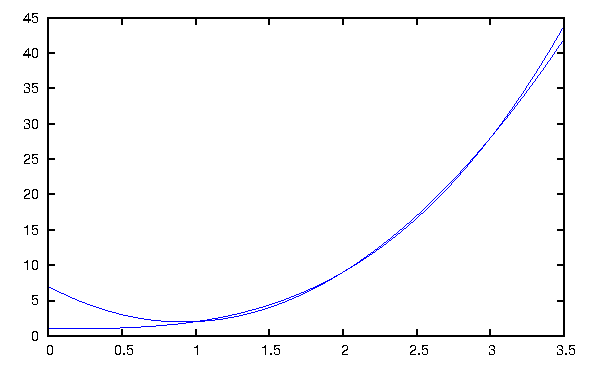
\includegraphics{figures/roots-polynomials02}.
\par\end{center}

\noindent$b\pm\sqrt{b^{2}-4ac}=25\pm\sqrt{625-672}=25\pm i\sqrt{47}$.
Karena $|25+i\sqrt{47}|=|25-i\sqrt{47}|$, akar mana pun dapat dipilih.
Dengan memilih $p_{3}=p_{2}-\frac{2c}{b-\sqrt{b^{2}-4ac}}$, diperoleh
$p_{3}=3-\frac{56}{25-i\sqrt{47}}=\frac{11}{12}-\frac{\sqrt{47}}{12}i$.
Jika proses ini dilanjutkan, diperoleh iterasi-iterasi $0.75238-0.75810i,\ 0.57069-0.84288i,\ldots,0.50000-0.86603i$,
yang konvergen ke $\frac{1}{2}-\frac{\sqrt{3}}{2}i$.

\begin{digression}{Orde Kekonvergenan}

\noindent\index{metode M�ller!orde kekonvergenan}Orde kekonvergenan
metode M�ller menuju akar sederhana (akar yang tidak berulang) adalah

\[
\left(\frac{\sqrt{11}}{3\sqrt{3}}+\frac{19}{27}\right)^{\frac{1}{3}}+\frac{4}{9\left(\frac{\sqrt{11}}{3\sqrt{3}}+\frac{19}{27}\right)^{\frac{1}{3}}}+\frac{1}{3}\approx1.839286755214161
\]
 dan menuju akar ganda adalah
\[
\left(\frac{\sqrt{139}}{24\sqrt{3}}+\frac{8}{27}\right)^{\frac{1}{3}}+\frac{7}{36\left(\frac{\sqrt{139}}{24\sqrt{3}}+\frac{8}{27}\right)^{\frac{1}{3}}}+\frac{1}{6}\approx1.233751928528259.
\]
 Metode Laguerre konvergen menuju akar sederhana dengan orde 3.
\begin{description}
\item [{Referensi}] \cite{muller,recipes}
\end{description}
\end{digression}

Tabel berikut merangkum keunggulan dan kelemahan relatif metode Newton,
metode sekan, dan metode M�ller.

\begin{center}
\begin{tabular}{c|ccc}
 & Newton & Sekan & M�ller\tabularnewline
\hline 
Nilai awal yang diperlukan & 1 & 2 & 3\tabularnewline
Perlu turunan? & Ya & Tidak & Tidak\tabularnewline
Orde Kekonvergenan\footnote{Orde yang dicantumkan berlaku untuk akar sederhana, bukan akar berulang.} & $2$ & $\approx1.618$ & $\approx1.839$\tabularnewline
Akar kompleks ditemukan secara otomatis? & Tidak & Tidak & Ya\tabularnewline
Lebih sederhana untuk polinom? & Ya & Tidak & Tidak\tabularnewline
\end{tabular}
\par\end{center}

\subsection{Konsep Utama}
\begin{description}
\item [{Pembagian~sintetis:}] \index{pembagian sintetis}Metode untuk
membagi polinom $p(x)$ dengan monomial $(x-x_{0})$ hanya dengan
menggunakan penjumlahan, perkalian, dan koefisien-koefisien $p$.
Proses ini identik dengan mengevaluasi polinom melalui penyarangan.
Pembagian sintetis sekadar menyediakan alat penataan agar penyarangan
dapat dilakukan dengan mudah menggunakan pensil dan kertas.
\item [{Metode~Horner:}] \index{metode Horner}Metode yang menghitung
nilai suatu polinom dan turunannya pada satu titik secara bersamaan
melalui pembagian sintetis.
\item [{Metode~M�ller:}] \index{metode M�ller}Metode pencarian akar yang
serupa dengan metode sekan, tetapi menggunakan parabola sebagai pengganti
garis sekan.
\item [{Deflasi:}] \index{deflasi}Metode untuk menyatakan suatu polinom
$p(x)$ sebagai hasil kali monomial $(x-x_{0})$ dan polinom $q(x)$
yang derajatnya satu lebih rendah daripada derajat polinom semula.
\end{description}
\startexercises 

\subsection{Latihan}
\begin{enumerate}
\item \label{exc:polynomials}\octave\ Tulislah sebuah fungsi Octave yang
menghitung akar-akar fungsi kuadrat dengan menggunakan bentuk alternatif
rumus kuadrat bila diperlukan. Baris pertama fungsi Anda harus berupa

\begin{center}
\texttt{function {[}r1,r2{]} = quadraticRoots(a,b,c)}
\par\end{center}

di mana \texttt{r1} dan \texttt{r2} merupakan akar-akar dari $p(x)=ax^{2}+bx+c$.
Dengan demikian, nilai \texttt{r1} dan \texttt{r2} dikembalikan oleh
fungsi dalam sebuah larik. Fungsi tersebut dipanggil seperti berikut:

\begin{center}
\texttt{{[}s,t{]}=quadraticRoots(1,2,3),}
\par\end{center}

yang menetapkan \texttt{s} sebagai nilai salah satu akar dan \texttt{t}
sebagai nilai akar lainnya. Uji kode Anda secara menyeluruh dengan
membandingkan keluaran fungsi Anda dengan hasil perhitungan manual
atau kalkulator.
\item \label{exc:polynomials-1}\octave\ Tulislah sebuah fungsi Octave
yang mengimplementasikan metode Horner. Baris pertama fungsi Anda
harus berupa 

\begin{center}
\texttt{function {[}p,pprime{]} = horner(x0,c)}
\par\end{center}

di mana \texttt{c} adalah larik yang memuat koefisien polinom, \texttt{x0}
adalah bilangan yang menjadi titik evaluasi polinom, \texttt{p} adalah
nilai polinom pada \texttt{x0}, dan \texttt{pprime} adalah nilai turunan
polinom pada \texttt{x0}. Dengan demikian, nilai \texttt{p} dan \texttt{pprime}
dikembalikan oleh fungsi dalam sebuah larik. Fungsi tersebut dipanggil
seperti berikut:

\begin{center}
\texttt{{[}y,yy{]}=horner(-2,{[}5,4,3,2,1{]}),}
\par\end{center}

yang menetapkan \texttt{y} sebagai nilai polinom dan \texttt{yy} sebagai
nilai turunannya. Uji kode Anda secara menyeluruh dengan membandingkan
keluaran fungsi Anda dengan hasil perhitungan manual atau kalkulator.
\item \label{exc:polynomials-2}\octave\ Tulislah sebuah fungsi Octave
yang mengimplementasikan metode Newton dengan metode Horner. Baris
pertama fungsi Anda harus berupa

\begin{center}
\texttt{function x = newtonhorner(c,x0,tol,N)}
\par\end{center}

di mana \texttt{c} adalah larik yang memuat koefisien polinom, \texttt{x0}
adalah nilai awal, \texttt{tol} adalah toleransi, dan \texttt{N} adalah
jumlah iterasi maksimum sebelum proses dihentikan. Kodenya harus serupa
dengan kode yang sebelumnya Anda tulis untuk mengimplementasikan metode
Newton, tetapi kode ini hanya berlaku untuk polinom. Di dalam fungsi
\texttt{newtonhorner}, JANGAN tuliskan kode metode Horner. Cukup panggil
fungsi \texttt{horner} yang Anda tulis pada soal \ref{exc:polynomials-1}.
Uji kode Anda secara menyeluruh dengan membandingkan keluaran fungsi
Anda dengan keluaran kode yang Anda tulis pada soal \ref{enu:newtonsMethodCode}
\vpageref{enu:newtonsMethodCode}.
\item \octave\ \label{exc:polynomials-12}Lengkapilah kode fungsi deflate
yang diawali di sini.\begin{verbatim}
% This function will deflate a polynomial
% given a root.
% INPUT: coefficients c of the polynomial;
%        a root r of the polynomial.
% OUTPUT: coefficients d of the deflated
%        polynomial.
function d = deflate(c,r)

end%function
\end{verbatim}
\item \octave\ Tulislah sebuah fungsi Octave yang mengimplementasikan metode
M�ller.
\item \label{exc:polynomials-3}Gunakan metode Horner/pembagian sintetis
untuk menentukan $g(2)$ dan $g'(2)$. Jangan gunakan komputer.

\begin{enumerate}
\item \label{exc:polynomials-6}$g(x)=3x^{3}+12x^{2}-13x-8$  \hasasolution 
\item \label{exc:polynomials-7}$g(x)=-7+8x-3x^{2}+5x^{3}-2x^{4}$ \hasananswer 
\end{enumerate}
\item \label{exc:polynomials-4}Gunakan metode Horner untuk menghitung $g(-2)$
dan $g'(-2)$ dengan $g(x)=4x^{4}-5x^{3}+6x-7$. Jangan gunakan komputer.
\item \label{exc:polynomials-10}Gunakan hasil pekerjaan Anda pada soal
\ref{exc:polynomials-3} untuk membantu melakukan dua iterasi metode
Newton dengan pensil, kertas, kalkulator, dan metode Horner/pembagian
sintetis. Gunakan nilai awal $x_{0}=2$. \haspartwithsolution  \haspartwithanswer 
\item Gunakan hasil pekerjaan Anda pada soal \ref{exc:polynomials-4} untuk
membantu melakukan dua iterasi metode Newton dengan pensil, kertas,
kalkulator, dan metode Horner/pembagian sintetis. Gunakan nilai awal
$x_{0}=-2$.
\item Hitung $x_{2}$ dari metode Newton secara manual (dengan menggunakan
metode Horner/pembagian sintetis) untuk $f(x)=x^{3}+4x-8$ dengan
nilai awal $x_{0}=0$.
\item Tentukan $x_{2}$ dari metode Newton secara manual (dengan menggunakan
metode Horner/pembagian sintetis) untuk $f(x)=x^{4}-2x^{3}-4x^{2}+4x+4$
dengan nilai awal $x_{0}=2$.
\item Dengan bantuan metode Horner dan tanpa menggunakan kalkulator, tentukan
iterasi pertama metode Newton untuk fungsi $f(x)=2x^{3}-10x+1$ dengan
nilai awal $x_{0}=2$.
\item Secara manual, tunjukkan dua iterasi metode Newton (dengan menggunakan
metode Horner/pembagian sintetis) yang diterapkan pada $f(x)=5x^{3}-2x^{2}+7x-3$
dengan $p_{0}=1$.
\item \label{findall}Carilah semua akar polinom dengan langkah-langkah
berikut. Gunakan metode Newton dengan toleransi $10^{-5}$ untuk menghampiri
salah satu akar polinom tersebut. Anda boleh menggunakan fungsi \texttt{newtonhorner}
yang Anda buat pada soal \ref{exc:polynomials-2}. Kemudian, gunakan
pembagian sintetis untuk melakukan deflasi pada polinom tersebut sehingga
derajatnya berkurang satu. Jangan gunakan komputer untuk deflasi.
Selanjutnya, gunakan metode Newton dengan toleransi $10^{-5}$ untuk
menghampiri salah satu akar polinom hasil deflasi. Kemudian, gunakan
kembali pembagian sintetis untuk melakukan deflasi pada polinom hasil
deflasi tersebut sehingga derajatnya berkurang satu lagi. Ulangi hingga
polinom hasil deflasi berderajat dua. Setelah itu, gunakan rumus kuadrat
(atau rumus kuadrat alternatif) untuk mencari dua akar terakhir.

\begin{enumerate}
\item \label{exc:polynomials-5}$g(x)=x^{4}+6x^{3}\text{\textminus}59x^{2}+144x\text{\textminus}144$ \hasasolution 
\item \label{exc:polynomials-14}$g(x)=-280+909x-154x^{2}-178x^{3}+54x^{4}+9x^{5}$ \hasananswer 
\end{enumerate}
\item Carilah semua akar polinom dengan langkah-langkah berikut. Gunakan
metode Newton dengan toleransi $10^{-5}$ untuk menghampiri salah
satu akar polinom tersebut. Anda boleh menggunakan fungsi \texttt{newtonhorner}
yang Anda buat pada soal \ref{exc:polynomials-2}. Kemudian, gunakan
pembagian sintetis untuk melakukan deflasi pada polinom tersebut sehingga
derajatnya berkurang satu. Anda boleh menggunakan fungsi \texttt{deflate}
yang Anda buat pada soal \ref{exc:polynomials-12} untuk proses deflasi
tersebut. Selanjutnya, gunakan metode Newton dengan toleransi $10^{-5}$
untuk menghampiri salah satu akar polinom hasil deflasi. Kemudian,
gunakan kembali pembagian sintetis untuk melakukan deflasi pada polinom
hasil deflasi tersebut sehingga derajatnya berkurang satu lagi. Ulangi
hingga polinom hasil deflasi berderajat dua. Setelah itu, gunakan
rumus kuadrat untuk mencari dua akar terakhir. Anda boleh menggunakan
fungsi \texttt{quadraticRoots} yang Anda buat pada soal \ref{exc:polynomials}
untuk menyelesaikan polinom kuadrat tersebut.

\begin{enumerate}
\item \label{exc:polynomials-16}$g(x)=x^{4}-2x^{3}-12x^{2}+16x-40$ \hasasolution 
\item \label{exc:polynomials-17}$g(x)=56-152x+140x^{2}-17x^{3}-48x^{4}+9x^{5}$ \hasananswer 
\end{enumerate}
\item \label{exc:polynomials-18}Untuk setiap akar yang Anda temukan pada
soal \ref{findall}, selain akar pertama, gunakan akar tersebut sebagai
hampiran awal dalam metode Newton dengan toleransi $10^{-5}$ untuk
melihat apakah Anda dapat memperbaiki hampiran akar tersebut. Apakah
hasilnya berubah? \haspartwithsolution  \haspartwithanswer 
\item $f(x)=x^{3}-1.255x^{2}-.9838x+1.2712$ memiliki akar di $x=1.12$.

\begin{enumerate}
\item Gunakan metode Newton dengan hampiran awal $x_{0}=1.13$ untuk mencoba
menemukan akar ini. Jelaskan apa yang terjadi.
\item Carilah semua akar $f(x)$.
\end{enumerate}
\item Sekitar 800 tahun lalu, John dari Palermo menantang para matematikawan
untuk mencari solusi persamaan $x^{3}+2x^{2}+10x=20$. Pada tahun
1224, Fibonacci menjawab tantangan tersebut di hadapan Kaisar Frederick
II. Ia menghampiri satu-satunya akar riil dengan teknik geometris
Omar Khayyam (1048-1131), hingga memperoleh taksiran
\[
\begin{gathered}1+22\left(\frac{1}{60}\right)+7\left(\frac{1}{60}\right)^{2}+42\left(\frac{1}{60}\right)^{3}+\\
\qquad\qquad33\left(\frac{1}{60}\right)^{4}+4\left(\frac{1}{60}\right)^{5}+40\left(\frac{1}{60}\right)^{6}.
\end{gathered}
\]
Seberapa akuratkah hampirannya?

\begin{description}
\item [{Referensi}] \cite[hlm. 96, soal 10]{burdenfaires}
\end{description}
\item \octave\ Hitung nilai polinom untuk nilai $x$ yang diberikan dengan
dua cara berbeda. (i) Gunakan fungsi \texttt{horner} yang Anda buat
pada soal \ref{exc:polynomials-1}; dan (ii) gunakan fungsi anonim.
Kemudian, (iii) bandingkan kedua hasil tersebut menggunakan operator
\texttt{==} pada Octave.

\begin{enumerate}
\item \label{exc:polynomials-8}$p(x)=x^{4}-2x^{3}-12x^{2}+16x-40$ pada
$x=\sqrt{3}$ \hasasolution 
\item \label{exc:polynomials-9}$q(x)=56-152x+140x^{2}-17x^{3}-48x^{4}+9x^{5}$
pada $x=\pi/2$ \hasananswer 
\item \label{exc:polynomials-11}$r(x)=x^{6}+11x^{4}-34x^{3}-130x^{2}-275x+819$
pada $\frac{1-\sqrt{5}}{2}$ \hasananswer 
\item $s(x)=5x^{10}+3x^{8}-46x^{6}-102x^{4}+365x^{2}+1287$ pada $\frac{1}{e}$
\end{enumerate}
\item \label{exc:polynomials-13}Tulislah fungsi Octave yang menggunakan
fungsi-fungsi Anda dari soal \ref{exc:polynomials}, \ref{exc:polynomials-2},
dan \ref{exc:polynomials-12} untuk mencari semua akar suatu polinom.
Uji fungsi Anda secara menyeluruh pada polinom-polinom dengan berbagai
derajat yang akar-akarnya telah Anda ketahui. Anda boleh mendasarkan
fungsi Anda pada kode semu \vpageref{pseudo:allroots}, tetapi kode
Anda seharusnya jauh lebih sederhana karena Anda cukup memanggil fungsi-fungsi
tersebut alih-alih menuliskan ulang kodenya. \hasananswer 
\item \label{exc:polynomials-15}Gunakan kode Anda dari soal \ref{exc:polynomials-13}
untuk mencari semua solusi persamaan berikut. \hasananswer 

\begin{enumerate}
\item $x^{5}+11x^{4}-34x^{3}-130x^{2}-275x+819=0$
\item $5x^{5}+3x^{4}-46x^{3}-102x^{2}+365x+1287=0$
\end{enumerate}
\item Carilah semua akar $g(x)=25x^{3}-105x^{2}+148x-174$.
\item Ingatlah bahwa metode sekan dan metode M�ller memiliki beberapa kemiripan.
Keduanya memerlukan beberapa hampiran awal. Keduanya melibatkan penentuan
nol suatu fungsi yang melalui titik-titik awal tersebut. Keduanya
konvergen secara superlinear menuju akar sederhana. Dan tentu saja,
keduanya merupakan metode pencarian akar. Mari kita ubah sedikit gagasan
ini sebagai berikut. Untuk mencari akar dari $g$, mulailah seperti
pada metode sekan dengan menggunakan dua hampiran, $x_{0}$ dan $x_{1}$.
Kemudian, alih-alih menggunakan nol dari garis yang melalui $(x_{0},g(x_{0}))$
dan $(x_{1},g(x_{1}))$, carilah fungsi berbentuk
\[
h(x)=ax^{3}+b
\]
yang melalui $(x_{0},g(x_{0}))$ dan $(x_{1},g(x_{1}))$. Misalkan
$x_{2}$ merupakan nol dari $h$. Kemudian, ulangi proses tersebut
dengan $x_{1}$ dan $x_{2}$ untuk memperoleh $x_{3}$, dan seterusnya.

\begin{enumerate}
\item Misalkan $g(x)=2\ln(1+x^{2})-x$, $x_{0}=5$, dan $x_{1}=6$. Tentukan
$x_{2}$ dengan menggunakan metode ini.
\item Carilah rumus untuk $x_{2}$ jika diberikan sebarang fungsi $g(x)$
dan sebarang kondisi awal $x_{0}$ dan $x_{1}$. Rumus tersebut harus
dinyatakan dalam $x_{0}$, $x_{1}$, $g(x_{0})$, dan $g(x_{1})$.
\item Carilah rumus umum untuk $x_{n}$ yang dinyatakan dalam $x_{n-2}$,
$x_{n-1}$, $g(x_{n-2})$, dan $g(x_{n-1})$.
\item \octave\ Tulislah fungsi Octave yang mengimplementasikan metode ini
dan menampilkan hasil setiap iterasi.
\item \octave\ Gunakan fungsi Octave Anda untuk menentukan apakah orde
kekonvergenan metode ini linear atau superlinear.
\end{enumerate}
\item Pilihlah fungsi yang akar-akarnya Anda ketahui secara eksak. Gunakan
metode M�ller untuk mencari salah satu akar tersebut. Gunakan tiga
iterasi berurutan untuk memperkirakan orde kekonvergenannya.
\item Galat dalam tiga iterasi berurutan metode M�ller ditampilkan dalam
tabel. Gunakan informasi ini untuk memperkirakan orde kekonvergenannya.

\begin{center}
\begin{tabular}{|c|c|}
\hline 
$n$ & $|x_{n}-x|$\tabularnewline
\hline 
\hline 
12 & $1.53627(10)^{-349}$\tabularnewline
\hline 
13 & $1.67365(10)^{-642}$\tabularnewline
\hline 
14 & $1.83922(10)^{-1181}$\tabularnewline
\hline 
\end{tabular}
\par\end{center}
\item \label{exc:polynomials-19}Grafik $f(x)$ ditampilkan. Carilah beberapa
himpunan nilai $p_{0}$, $p_{1}$, dan $p_{2}$ yang berbeda satu
sama lain, sehingga metode M\"uller

\begin{enumerate}
\item akan menghasilkan nilai kompleks untuk $p_{3}$.
\item akan menghasilkan akar di $x\approx4.4$.
\item akan menghasilkan akar di $x\approx2.8$.
\end{enumerate}
\begin{center}
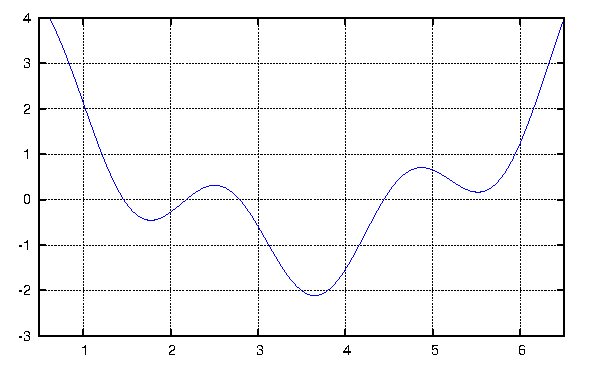
\includegraphics[scale=0.7]{figures/roots-polynomials01}
\par\end{center}
\item \octave\ Fungsi yang ditampilkan pada soal \ref{exc:polynomials-19}
adalah $f(x)=\frac{x^{2}-7x+10}{2}+\sin(3x)$. Gunakan informasi ini
untuk menguji dugaan-dugaan Anda pada soal \ref{exc:polynomials-19}.
\end{enumerate}
\finishexercises 



\section{\label{sec:RootsBracketing}Pengurungan\index{pengurungan}}

Metode bagi dua disebut metode pencarian akar dengan pengurungan.
Sebuah akar diketahui berada di dalam suatu selang tertentu. Setiap
iterasi memperkecil lebar selang sambil mempertahankan jaminan bahwa
akar tetap berada di dalamnya. Pada setiap langkah algoritme, akar
diketahui berada di antara hampiran terbaru dan salah satu hampiran
sebelumnya. Kedua batas ini membentuk selang pengurung bagi akar.
Seiring berjalannya algoritme, lebar selang pengurung menyusut hingga
lebih kecil daripada toleransi tertentu; pada saat itu akar diketahui
sudah dekat dan algoritme berhenti.

Kelemahan metode bagi dua adalah orde kekonvergenannya yang linear.
Dibandingkan dengan metode superlinear seperti metode sekan dan metode
Newton, metode bagi dua bergerak sangat lambat. Namun, metode bagi
dua memiliki sesuatu yang tidak dimiliki metode sekan dan metode Newton---kepastian
kekonvergenan. Memang, metode sekan dan metode Newton cepat ketika
konvergen, tetapi tidak ada jaminan bahwa keduanya akan konvergen.

Metode yang menggabungkan keunggulan metode bagi dua (kekonvergenan
terjamin) dengan metode berorde lebih tinggi (kecepatan) disebut metode
berpengaman. Metode tersebut dijamin konvergen dan dapat melakukannya
dengan cepat ketika hampiran sudah dekat dengan akar. Setiap metode
superlinear dapat dilengkapi dengan pengurungan sehingga menghasilkan
metode berpengaman.

\subsection{Pengurungan}

Pengurungan berarti mempertahankan suatu selang yang diketahui memuat
akar. Pengurungan digunakan dalam metode bagi dua. Pada setiap iterasi,
akar diketahui berada di antara dua hampiran terbaru. Pengurungan
tidak digunakan dalam metode sekan maupun metode Newton. Tidak ada
jaminan bahwa akar tetap dekat dengan hampiran-hampiran terbaru. 

Meskipun demikian, tidaklah sulit untuk menggabungkan metode bagi
dua dengan metode sekan, metode Newton, atau metode berorde tinggi
lainnya, guna membentuk metode hibrida yang menjaga akar tetap terkurung
sekaligus membuka peluang bagi kekonvergenan cepat. Dalam metode seperti
ini, kandidat hampiran berikutnya dihitung menurut metode berorde
tinggi. Jika kandidat berada di dalam selang pengurung, kandidat itu
menjadi hampiran berikutnya. Jika kandidat berada di luar selang pengurung,
metode bagi dua digunakan untuk menghitung hampiran berikutnya sebagai
gantinya.

Metode sekan terkurung\index{metode sekan terkurung}, yang lebih
dikenal sebagai metode posisi palsu atau regula falsi, memberikan
contoh sederhana. Bahkan, metode berorde tinggi (metode sekan) selalu
menghasilkan nilai di dalam selang pengurung, sehingga titik tersebut
tidak perlu diperiksa. Perbedaan antara posisi palsu dan metode sekan
terletak pada pemilihan salah satu dari dua hampiran sebelumnya yang
akan dipertahankan. Dalam metode sekan, hampiran terbarulah yang selalu
dipertahankan untuk langkah berikutnya. Dalam posisi palsu, hampiran
yang mempertahankan selang pengurung bagi akar dipertahankan untuk
langkah berikutnya, baik hampiran itu yang paling baru maupun bukan.
Metode Newton terkurung\index{metode Newton terkurung} memberikan
contoh yang sedikit lebih lanjut karena sangat mungkin hampiran yang
dihasilkan metode Newton jatuh di luar selang pengurung.

Ambil fungsi $g(x)=3-x-\sin(x)$ pada selang $[2,3]$. $f$ kontinu
pada $[2,3]$, dan $g(2)\approx0.09$ serta $g(3)\approx-0.14$ berlainan
tanda. Jadi, $[2,3]$ mengurung sebuah akar $g$; karena itu, tetapkan
$x_{0}=2$ dan $x_{1}=3$. Tabel berikut menunjukkan perhitungan hampiran
berikutnya untuk metode sekan terkurung dan metode Newton terkurung.

\begin{center}
\begin{tabular}{c|cccc}
 & $x_{0}$ & $x_{1}$ & kandidat $x_{2}$ & $x_{2}$\tabularnewline
\hline 
sekan terkurung & $2$ & $3$ & $x_{1}-g(x_{1})\frac{x_{1}-x_{0}}{g(x_{1})-g(x_{0})}\approx2.3912$ & $2.3912$\tabularnewline
Newton terkurung & $2$ & $3$ & $x_{1}-\frac{g(x_{1})}{g'(x_{1})}\approx-11.101$ & $2.5$\tabularnewline
\end{tabular}
\par\end{center}

\noindent Dalam metode sekan terkurung, kandidat $x_{2}$ diterima,
tetapi dalam metode Newton terkurung, kandidat $x_{2}$ berada di
luar selang pengurung sehingga dibuang, dan $x_{2}$ menurut metode
bagi dua ($2.5$) digunakan sebagai gantinya.

Untuk menyiapkan hampiran berikutnya, $g(x_{2})$ dihitung. Karena
$g(x_{2})$ bernilai negatif pada kedua metode, $x_{1}$ lama, yaitu
$3$, dibuang dan $x_{0}=2$ ``dipromosikan'' menjadi $x_{1}$ untuk
mempertahankan selang pengurung. Dengan cara ini, $g$ berlainan tanda
di $x_{1}$ dan $x_{2}$. Tabel berikut memperlihatkan proses pengambilan
keputusan ini sekaligus perhitungan hampiran berikutnya.

\begin{center}
\begin{tabular}{c|ccccc}
 & $g(x_{2})$ & $x_{1}$ & $x_{2}$ & kandidat $x_{3}$ & $x_{3}$\tabularnewline
\hline 
sekan terkurung & $-0.073141$ & $2$ & $2.3912$ & $x_{2}-g(x_{2})\frac{x_{2}-x_{1}}{g(x_{2})-g(x_{1})}\approx2.2165$ & $2.2165$\tabularnewline
Newton terkurung & $-0.098472$ & $2$ & $2.5$ & $x_{2}-\frac{g(x_{2})}{g'(x_{2})}\approx2.0048$ & $2.0048$\tabularnewline
\end{tabular}
\par\end{center}

\noindent Dapatkah Anda melengkapi nilai $x_{4}$ berdasarkan nilai-nilai
dalam tabel berikut? Perhatikan bahwa $x_{1}$ lama harus ``dipromosikan''
pada metode sekan terkurung, tetapi tidak pada metode Newton terkurung.
Mengapa? Jawaban \vpageref{ans:bracketedx4}.

\begin{center}
\begin{tabular}{c|ccccc}
 & $g(x_{3})$ & $x_{2}$ & $x_{3}$ & kandidat $x_{4}$ & $x_{4}$\tabularnewline
\hline 
sekan terkurung & $-0.015215$ & $2$ & $2.2165$ & $x_{3}-g(x_{3})\frac{x_{3}-x_{2}}{g(x_{3})-g(x_{2})}\approx2.1854$ & ?\tabularnewline
Newton terkurung & $0.087906$ & $2.5$ & $2.0048$ & $x_{3}-\frac{g(x_{3})}{g'(x_{3})}\approx2.1565$ & ?\tabularnewline
\end{tabular}
\par\end{center}

\noindent 5 hampiran berikutnya dari setiap metode diberikan di sini
jika Anda ingin mencoba menghitung beberapa di antaranya sendiri.
Sekarang adalah saat yang tepat untuk melakukannya. Nilai-nilai ini
dihitung menggunakan kode Octave berikut.

\begin{center}
\begin{tabular}{c|cc}
 & \multicolumn{2}{c}{terkurung}\tabularnewline
 & sekan & Newton\tabularnewline
\hline 
$x_{5}$ & $2.18062942638407$ & $2.17925592233708$\tabularnewline
$x_{6}$ & $2.17988957044102$ & $2.17975682599184$\tabularnewline
$x_{7}$ & $2.17977718322867$ & $2.17975706647997$\tabularnewline
$x_{8}$ & $2.17976012038625$ & $2.17975706648003$\tabularnewline
$x_{9}$ & $2.17975753008587$ & $2.17975706648003$\tabularnewline
\end{tabular}
\par\end{center}

\subsubsection{Kode Octave untuk Posisi Palsu (Metode Sekan Terkurung)\index{metode sekan terkurung!kode Octave}}

\noindent\begin{verbatim}
%%%%%%%%%%%%%%%%%%%%%%%%%%%%%%%%%%%%%%%%%%%%%%%%%
% Written by Dr. Len Brin           20 May 2014 %
% Purpose: Implementation of the Method of      %
%        False Position.                        %
% INPUT: function g; initial values a and b;    %
%        tolerance TOL; maximum iterations N    %
% OUTPUT: approximation x and number of         %
%        iterations i; or message of failure    %
%%%%%%%%%%%%%%%%%%%%%%%%%%%%%%%%%%%%%%%%%%%%%%%%%
function [x,i] = falsePosition(g,a,b,TOL,N)
  i=1;
  A=g(a);
  B=g(b);
  while (i<N)
    b
    x=b-B*(b-a)/(B-A);
    if (abs(x-b)<TOL)
      return
    end%if
    X=g(x);
    if ((B<0 && X>0) || (B>0 && X<0))
      a=b; A=B;
    end%if
    b=x; B=X;
    i=i+1;
  end%while
  x="Method failed---maximum number of iterations reached";
end%function
\end{verbatim}

\subsubsection{Kode Octave untuk Metode Newton Terkurung\index{metode Newton terkurung!kode Octave}}

\noindent\begin{verbatim}
%%%%%%%%%%%%%%%%%%%%%%%%%%%%%%%%%%%%%%%%%%%%%%%%%
% Written by Dr. Len Brin           20 May 2014 %
% Purpose: Implementation of bracketed Newton's %
%        method.                                %
% INPUT: function g; its derivative gp; initial %
%        values a and b; tolerance TOL; maximum %
%        iterations N                           %
% OUTPUT: approximation x and number of         %
%        iterations i; or message of failure    %
%%%%%%%%%%%%%%%%%%%%%%%%%%%%%%%%%%%%%%%%%%%%%%%%%
function [x,i] = bracketedNewton(g,gp,a,b,TOL,N)
  i=1;
  A=g(a);
  B=g(b);
  while (i<N)
    b
    x=b-B/gp(b);
    if (x<min([a,b]) || x>max([a,b]))
      x=b+(a-b)/2;
    end%if
    if (abs(x-b)<TOL)
      return
    end%if
    X=g(x);
    if ((B<0 && X>0) || (B>0 && X<0))
      a=b; A=B;
    end%if
    b=x; B=X;
    i=i+1;
  end%while
  x="Method failed---maximum number of iterations reached";
end%function
\end{verbatim}\texttt{falsePosition.m} dan \texttt{bracketedNewton.m} dapat diunduh
dari \href{http://lqbrin.github.io/tea-time-numerical/ancillaries.html}{situs pendamping}.

Kode untuk metode sekan terkurung dan metode Newton terkurung sangat
mirip. Bahkan, keduanya hampir identik. Hanya ada dua perbedaan selain
komentar pada bagian awal. Metode sekan terkurung menggunakan baris
\texttt{x=b-B{*}(b-a)/(B-A);}, sedangkan metode Newton terkurung menggunakan
baris \texttt{x=b-B/gp(b);}. Inilah perbedaan mendasar antara keduanya
karena pada bagian inilah metode berorde tinggi dijalankan. Satu-satunya
perbedaan lain adalah metode Newton terkurung menyertakan tiga baris
yang memeriksa apakah \texttt{x} berada di dalam selang pengurung
dan menjalankan satu langkah metode bagi dua jika tidak:

\noindent\begin{verbatim}
    if (x<min([a,b]) || x>max([a,b]))
      x=b+(a-b)/2;
    end%if
\end{verbatim}

\noindent Sebenarnya, kita dapat menambahkan ketiga baris ini ke metode
sekan terkurung dan program akan berjalan sama saja. Metode sekan
tidak mungkin menghasilkan nilai \texttt{x} di luar selang pengurung,
sehingga langkah bagi dua tidak akan pernah dijalankan. Satu-satunya
perbedaan mendasar antara kedua fungsi adalah pelaksanaan metode berorde
tinggi.

Kita dapat menggunakan pengamatan ini untuk membuat semacam cetak
biru bagi pengurungan metode berorde tinggi apa pun. Metode Steffensen,
metode M�ller (selama hampiran tetap riil), atau metode Sidi (Bagian
\ref{sec:polynomialLagrange}), misalnya, dapat diberi pengurungan
dengan cara ini. Kode semu-semu berikut menyajikan cetak biru tersebut
dan memberi panduan untuk mengamankan metode berorde tinggi dengan
menggabungkannya dengan metode bagi dua.

\noindent\begin{pseudocode}\label{pseudo:safeguarded}\index{pengurungan!kode semu}
\begin{description}
\item [{Asumsi:}] $g$ kontinu pada $[a,b]$. $g(a)$ dan $g(b)$ berlainan
tanda.
\item [{Masukan:}] Selang $[a,b]$; fungsi $g$; akurasi yang diinginkan
$tol$; jumlah maksimum iterasi $N$; variabel lain yang diperlukan
untuk menjalankan iterasi metode superlinear, seperti $g'$ dalam
metode Newton.
\item [{Langkah~1:}] Tetapkan $A=g(a)$; $B=g(b)$; $i=2$;
\item [{Langkah~2:}] Inisialisasikan variabel lain yang diperlukan untuk
superlinear();
\item [{Langkah~3:}] Selama $i<N$, lakukan Langkah 4--10:

\begin{description}
\item [{Langkah~4:}] Tetapkan $x=\mbox{superlinear}(a,b,g,\ldots)$;
\item [{Langkah~5:}] Jika $(x-a)(x-b)>0$, maka $x=b+\frac{a-b}{2}$;
\item [{Langkah~6:}] Jika $|x-b|<tol$, kembalikan $x$
\item [{Langkah~7:}] Tetapkan $X=g(x)$;
\item [{Langkah~8:}] Jika $BX<0$, tetapkan $a=b$; $A=B$;
\item [{Langkah~9:}] Tetapkan $b=x$; $B=X$; $i=i+1$;
\item [{Langkah~10:}] Perbarui variabel lain yang diperlukan untuk superlinear();
\end{description}
\item [{Langkah~11:}] Cetak ``Metode gagal. Jumlah maksimum iterasi terlampaui.''
\item [{Keluaran:}] Hampiran $m$ yang berjarak kurang dari $tol$ dari
akar eksak, atau pesan kegagalan.
\end{description}
\end{pseudocode}

Sebagai alasan perlunya mengembangkan versi metode orde tinggi lain
yang memakai selang pengurung, perhatikan fungsi yang sangat bermasalah
$g(x)=\frac{1+10x}{1-10x}$. Fungsi ini berakar di $-\frac{1}{10}$,
tetapi metode sekan dengan selang pengurung dapat sangat lambat konvergen
menuju akar ini. Gambar \ref{fig:troubleForSecant} 
\begin{figure}
\caption{\label{fig:troubleForSecant}Fungsi yang menyulitkan metode sekan
dengan selang pengurung.}

\centering{}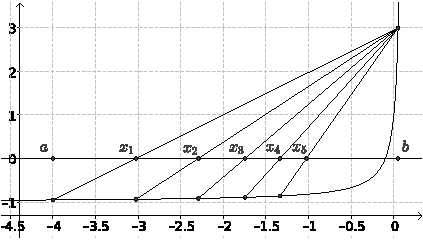
\includegraphics{figures/rootBracketing01}
\end{figure}
 memperlihatkan kekonvergenan lambat ini jika dimulai dengan selang
pengurung $[a,b]=[-4,.05]$. Dengan pilihan selang pengurung yang
kurang tepat ini, metode membutuhkan 45 iterasi untuk mencapai akurasi
$10^{-5}$. Algoritma yang lebih cerdas tidak hanya memeriksa bahwa
setiap hampiran berada di dalam selang pengurung, tetapi juga memastikan
bahwa metode orde tinggi bergerak cukup cepat menuju akar. Jika algoritma
mendeteksi kekonvergenan yang lambat, misalnya lebih lambat daripada
metode bagi dua, algoritma akan menggunakan langkah bagi dua sebagai
gantinya. Perhatikan bahwa metode Newton dengan selang pengurung tidak
mengalami masalah berarti pada fungsi ini. Dengan selang pengurung
awal yang sama, metode tersebut mencapai jarak $10^{-5}$ dari akar
hanya dalam 10 iterasi (empat iterasi pertamanya merupakan langkah
bagi dua). Sayangnya, metode Newton memerlukan turunan. Metode cepat
untuk mencari akar dalam selang pengurung tanpa memerlukan turunan
akan sangat berguna.

Pada awal 1970-an, Richard Brent\index{metode Brent}\index{metode!Brent|see{metode Brent}}
mengembangkan karya van Wijngaarden dan Dekker menjadi metode dengan
selang pengurung yang memadukan metode bagi dua, metode sekan, dan
interpolasi kuadratik invers, sambil terus memeriksa bahwa metode
orde tinggi bergerak cukup cepat menuju akar. Hasilnya kini dikenal
sebagai metode Brent \cite{brent}. Metode ini tidak memerlukan turunan.
Metode ini cepat. Kekonvergenannya dijamin. Karena itu, metode ini
populer sebagai metode serbaguna untuk mencari akar dalam selang pengurung
ketika turunan tidak tersedia. Rincian lengkap metode Brent tidak
akan disajikan di sini, tetapi satu langkah penting menuju metode
tersebut akan disajikan. Metode yang disajikan di sini mirip dengan
fungsi MATLAB \texttt{fzero} \cite{moler}.

\subsection{Interpolasi Kuadratik Invers\index{metode interpolasi kuadratik invers}}

Seperti yang mungkin Anda ingat, metode M�ller memerlukan tiga hampiran
awal, misalnya $a$, $b$, dan $c$. Parabola yang melalui titik $(a,g(a))$,
$(b,g(b))$, dan $(c,g(c))$ digambar, dan titik potongnya dengan
sumbu $x$ menghasilkan hampiran berikutnya. Unsur kunci metode ini---proses
mencocokkan fungsi kuadrat dengan ketiga titik---disebut interpolasi.
Dengan demikian, metode M�ller juga dapat disebut ``metode interpolasi
kuadratik''.

Seperti dapat diduga, metode interpolasi kuadratik invers serupa.
Alih-alih mencocokkan fungsi kuadrat dengan titik $(a,g(a))$, $(b,g(b))$,
dan $(c,g(c))$, peran $x$ dan $y$ dipertukarkan. Sebagai gantinya,
fungsi kuadrat dicocokkan dengan titik $(g(a),a)$, $(g(b),b)$, dan
$(g(c),c)$. Karena dalam kasus ini $x$ merupakan fungsi dari $y$,
grafik fungsi kuadrat itu akan memotong sumbu $x$ tepat sekali, yakni
saat $y=0$. Mengevaluasi fungsi kuadrat di $0$ menghasilkan hampiran
berikutnya. Gambar \ref{fig:quadraticVSinverseQuadratic} memperlihatkan
interpolasi kuadratik dan interpolasi kuadratik invers pada himpunan
tiga titik yang sama. Dalam interpolasi kuadratik, $y$ diperlakukan
sebagai fungsi dari $x$. Dalam interpolasi kuadratik invers, $x$
diperlakukan sebagai fungsi dari $y$. Interpolasi kuadratik invers
menghindari komplikasi utama interpolasi kuadratik---menghitung titik
potongnya dengan sumbu $x$. Dalam interpolasi kuadratik, fungsi kuadrat
mungkin memotong sumbu $x$ dua kali atau sama sekali tidak memotongnya!
Dalam kedua kasus, suatu pilihan harus dibuat pada setiap langkah,
dan akar-akar fungsi kuadrat melibatkan rumus kuadrat. Dalam interpolasi
kuadratik invers, fungsi kuadrat dijamin memotong sumbu $x$ tepat
sekali, dan titik potong itu cukup dicari dengan mengevaluasi fungsi
kuadrat di $0$. Artinya, $y=0$. Ingat, fungsi kuadrat memberikan
$x$ sebagai fungsi dari $y$.

Dengan merujuk kembali pada penurunan metode M�ller \vpageref{subsec:mullers},
jika parabola dipaksa melalui titik $(a,A)$, $(b,B)$, dan $(c,C)$,
lalu peran $x$ dan $y$ dipertukarkan, rumus untuk parabola invers
$q$ langsung diperoleh:

\[
q(y)=q_{0}(y-B)^{2}+q_{1}(y-B)+q_{2}
\]
dengan
\begin{eqnarray*}
q_{2} & = & b\\
q_{1} & = & \frac{(A-B)^{2}(c-b)-(C-B)^{2}(a-b)}{(A-B)(C-B)(A-C)}\\
q_{0} & = & \frac{(C-B)(a-b)-(A-B)(c-b)}{(A-B)(C-B)(A-C)}.
\end{eqnarray*}
\begin{digression}{Orde kekonvergenan interpolasi kuadratik} 

\noindent Metode interpolasi kuadratik invers\index{metode interpolasi kuadratik invers!orde kekonvergenan}
memiliki orde kekonvergenan sekitar $1.84$ dengan asumsi yang wajar.
Jika fungsi yang akarnya dicari memiliki tiga turunan kontinu di suatu
lingkungan akar, tiga hampiran terbaru cukup dekat, dan akarnya sederhana,
orde kekonvergenannya adalah solusi riil dari 
\[
\alpha^{3}-\alpha^{2}-\alpha-1=0.
\]
Kita dapat menggunakan interpolasi kuadratik invers untuk menghampirinya!
\begin{verbatim}
>> format('long')
>> f=@(x) x^3-x^2-x-1
f =
@(x) x ^ 3 - x ^ 2 - x - 1
>> [res,i]=inverseQuadratic(f,1,2,10^-12,100)
res =  1.83928675521416
i =  8
\end{verbatim} Solusi eksaknya adalah
\[
\alpha=\left(\frac{\sqrt{11}}{3\sqrt{3}}+\frac{19}{27}\right)^{\frac{1}{3}}+\frac{4}{9\left(\frac{\sqrt{11}}{3\sqrt{3}}+\frac{19}{27}\right)^{\frac{1}{3}}}+\frac{1}{3}.
\]
Anda mungkin mengenali nilai ini sebagai orde kekonvergenan metode
M�ller. Memang, setiap metode interpolasi kuadratik konvergen menuju
akar sederhana dengan orde ini.
\begin{description}
\item [{Referensi}] \cite{sharma}
\end{description}
\noindent\end{digression} 

Dengan demikian, titik potong dengan sumbu $x$ adalah 
\begin{eqnarray*}
x & = & q(0)\\
 & = & B^{2}q_{0}-Bq_{1}+q_{2}\\
 & = & B^{2}\frac{(C-B)(a-b)-(A-B)(c-b)}{(A-B)(C-B)(A-C)}-B\frac{(A-B)^{2}(c-b)-(C-B)^{2}(a-b)}{(A-B)(C-B)(A-C)}+b\\
 & = & \frac{\left[B^{2}(C-B)+B(C-B)^{2}\right](a-b)-\left[B^{2}(A-B)+B(A-B)^{2}\right](c-b)}{(A-B)(C-B)(A-C)}+b\\
 & = & \frac{\left[-B^{2}C+BC^{2}\right](a-b)-\left[-B^{2}A+BA^{2}\right](c-b)}{(A-B)(C-B)(A-C)}+b\\
 & = & \frac{BC(C-B)(a-b)-BA(A-B)(c-b)}{(A-B)(C-B)(A-C)}+b\\
 & = & b+\frac{\frac{B}{A}(\frac{C}{B}-1)(a-b)-\frac{A}{C}(1-\frac{B}{A})(c-b)}{(1-\frac{B}{A})(\frac{C}{B}-1)(\frac{A}{C}-1)}\\
 & = & b+\frac{\frac{A}{C}(1-\frac{B}{A})(c-b)-\frac{B}{A}(\frac{C}{B}-1)(a-b)}{(\frac{B}{A}-1)(\frac{B}{C}-1)(\frac{A}{C}-1)}.
\end{eqnarray*}
Agar perhitungan $x$ sedikit lebih mudah diprogram, diperkenalkan
beberapa variabel baru. Misalkan
\[
r=\frac{B}{A}-1,\quad s=\frac{C}{B}-1,\quad t=\frac{A}{C}-1
\]
sehingga
\begin{equation}
x=b-\frac{r(t+1)(c-b)+s(r+1)(a-b)}{rst}.\label{eq:inverseQuadratic}
\end{equation}

\begin{figure}
\caption{\label{fig:quadraticVSinverseQuadratic}Interpolasi kuadratik dan
interpolasi kuadratik invers.}

\centering{}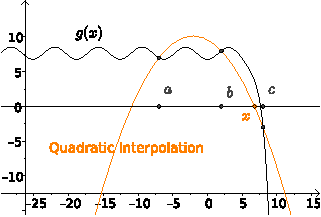
\includegraphics{figures/rootBracketing02}\qquad{}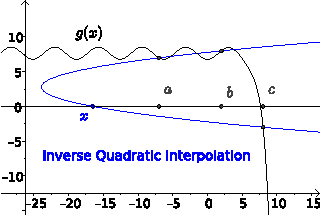
\includegraphics{figures/rootBracketing03}
\end{figure}

Interpolasi kuadratik invers dapat dilengkapi selang pengurung seperti
metode orde tinggi lainnya. Namun, metode ini menimbulkan pertanyaan
menarik yang tidak muncul pada semua metode orde tinggi. Interpolasi
kuadratik memerlukan tiga titik; ketika ketiganya digunakan untuk
menghasilkan hampiran berikutnya, terbentuk titik keempat. Dari keempat
titik itu, komputer harus menentukan dua titik yang akan menjadi selang
pengurung berikutnya dan satu titik yang akan menjadi titik ketiga
untuk interpolasi berikutnya. Namun, kita sudah melangkah terlalu
jauh.

Setiap iterasi dimulai dengan tiga titik, $(a,g(a))$, $(b,g(b))$,
dan $(c,g(c))$, dengan $a$ dan $b$ mengurung sebuah akar, sedangkan
$c$ merupakan titik ketiga. Pada iterasi pertama, hanya selang pengurung
yang diberikan. $c$ disamakan dengan $a$. Pada setiap iterasi, tanda
$g(a)$ dan $g(b)$ diperiksa untuk memastikan bahwa $a$ dan $b$
mengurung sebuah akar. Jika tandanya berlainan, metode dilanjutkan.
Jika tandanya sama, berarti $g(b)$ dan $g(c)$ pasti berlainan tanda,
sehingga $a$ disamakan dengan $c$. Selanjutnya, nilai mutlak $g(a)$
dan $g(b)$ diperiksa. Jika $|g(a)|<|g(b)|$, label $a$ dan $b$
dipertukarkan dan $c$ disamakan dengan nilai baru $a$. Setelah pemeriksaan
awal ini, perhitungan hampiran berikutnya dimulai dengan jaminan bahwa
sebuah akar terletak di antara $a$ dan $b$; $b$ kemungkinan merupakan
taksiran akar terbaik sejauh ini; dan $c$ kemungkinan merupakan taksiran
akar terburuk sejauh ini.

Jika $c=a$ setelah pemeriksaan awal dan kemungkinan pelabelan ulang,
interpolasi kuadratik tidak dapat dilakukan. Hampiran berikutnya dihasilkan
dengan metode sekan (interpolasi linear). Jika $c\neq a$ setelah
pemeriksaan awal dan kemungkinan pelabelan ulang, calon hampiran berikutnya,
$x$, dihitung menggunakan interpolasi kuadratik invers. Jika calon
tersebut berada di dalam selang pengurung, calon itu diterima sebagai
hampiran berikutnya. Jika berada di luar selang pengurung, langkah
metode bagi dua digunakan sebagai gantinya. Dalam kedua kasus, $c$
disamakan dengan $b$ dan $b$ disamakan dengan $x$. Untuk interpolasi
kuadratik invers dengan selang pengurung, hal ini menuntaskan satu
iterasi. Metode kemudian diulang sampai ditemukan hampiran yang cukup
baik.

Dalam skenario terbaik, interpolasi kuadratik invers digunakan pada
setiap langkah dan kekonvergenannya superlinear dengan orde sekitar
$1.84$. Dalam skenario terburuk, salah satu metode orde tinggi digunakan
pada setiap langkah, tetapi fungsinya patologis dan kekonvergenannya
lambat, bahkan mungkin lebih lambat daripada metode bagi dua. Meskipun
demikian, kekonvergenan lambat jarang terjadi, dan orde kekonvergenan
aktual secara umum tidak dapat ditentukan secara pasti. Metode ini
berganti-ganti antara metode yang berbeda orde. Yang dapat kita katakan
hanyalah bahwa biasanya metode ini cepat.

\subsubsection{Kode Octave untuk Interpolasi Kuadratik Invers dengan Selang Pengurung\index{interpolasi kuadratik invers dengan selang pengurung!kode Octave}}

\begin{verbatim}
%%%%%%%%%%%%%%%%%%%%%%%%%%%%%%%%%%%%%%%%%%%%%%%%%
% Written by Dr. Len Brin           21 May 2014 %
% Purpose: Implementation of bracketed inverse  %
%        quadratic interpolation method.        %
% INPUT: function g; initial values a and b;    %
%        tolerance TOL; maximum iterations N0   %
% OUTPUT: approximation x and number of         %
%        iterations i; or message of failure    %
%%%%%%%%%%%%%%%%%%%%%%%%%%%%%%%%%%%%%%%%%%%%%%%%%
function [x,i] = bracketedInverseQuadratic(g,a,b,TOL,N0)
  i=1;
  A=g(a);
  B=g(b);
  c=a; C=A;
  while (i<N0)
    b
    if (B*A>0)
      a=c; A=C;
    end%if
    if (abs(A) < abs(B))
      c=b; C=B;
      b=a; B=A;
      a=c; A=C;
    end%if
    if (a==c)
      x=(b*A-a*B)/(A-B);
    else
      r=B/A-1; s=C/B-1; t=A/C-1;
      p=(t+1)*r*(c-b)+(r+1)*s*(a-b);
      q=t*s*r;
      x=b-p/q;
    end%if
    if (x<min([a,b]) || x>max([a,b]))
      x=b+(a-b)/2;
    end%if
    if (abs(x-b)<TOL)
      disp(" ");
      return
    end%if
    c=b; C=B;
    b=x; B=g(b);
    i=i+1;
  end%while
  x="Method failed---maximum number of iterations reached";
end%function
\end{verbatim} Penerapan metode interpolasi kuadratik invers dengan selang pengurung
pada fungsi bermasalah $g(x)=\frac{1+10x}{1-10x}$ di selang $[-4,.05]$
menghasilkan akurasi $10^{-5}$ hanya dalam 11 iterasi. Metode ini
hanya membutuhkan satu iterasi lebih banyak daripada metode Newton
dengan selang pengurung, tanpa memerlukan turunan $g$! \texttt{bracketedInverseQuadratic.m}
dapat diunduh dari \href{http://lqbrin.github.io/tea-time-numerical/ancillaries.html}{situs pendamping}.

\subsection{Penghentian\index{kriteria penghentian!untuk pencarian akar}}

Dalam semua metode pencarian akar kita, algoritme berhenti ketika
selisih antara dua hampiran berturut-turut lebih kecil daripada toleransi
tertentu. Kriteria ini didasarkan pada asumsi bahwa galat tidak akan
melebihi selisih tersebut. Asumsi itu aman bagi setiap metode yang
sedang konvergen secara superlinear ketika berhenti. Bahkan, asumsi
itu juga aman bagi metode bagi dua yang konvergen secara linear, karena
selisih antara dua hampiran berturut-turut tepat sama dengan batas
teoretis galat. 

Kriteria ini tidak aman ketika metode superlinear digunakan begitu
jauh dari akar sehingga kekonvergenan superlinear tidak tampak. Inilah
tepatnya yang terjadi pada Gambar \vpageref{fig:troubleForSecant}.
Selisih antara hampiran-hampiran berturut-turut sebenarnya lebih besar
daripada galat absolut pada setiap langkah. Situasi ini tidak lazim,
tetapi dapat terjadi. 

Kriteria ini juga tidak aman ketika suatu metode konvergen secara
linear dengan konstanta kekonvergenan asimtotik $\lambda>\frac{1}{2}$.
Namun, metode yang konvergen secara linear sebaiknya tidak pernah
digunakan sendiri karena selalu ada alternatif yang lebih cepat.

Ada satu pertimbangan penting lagi mengenai penghentian. Berhenti
ketika selisih antara dua hampiran berturut-turut lebih kecil daripada
toleransi tertentu bergantung pada galat absolut. Ketika akar mungkin
sangat kecil atau sangat besar, barangkali lebih baik menggunakan
kriteria berdasarkan galat relatif. Sebagai contoh, alih-alih berhenti
ketika $|x_{n+1}-x_{n}|<tol$, kita berhenti ketika $|x_{n+1}-x_{n}|<tol\cdot|x_{n+1}|$.

\subsection{Konsep Kunci}
\begin{description}
\item [{Pengurungan:}] \index{pengurungan}Memperhalus secara iteratif
suatu selang---yang juga disebut selang pengurung---yang diketahui
memuat akar, hingga lebarnya lebih kecil daripada toleransi tertentu.
\item [{Interpolasi~kuadratik~invers:}] \index{metode interpolasi kuadratik invers}\index{metode!interpolasi kuadratik invers|see{metode interpolasi kuadratik invers}}Sebuah
polinom kuadrat dalam $y$ dicocokkan dengan tiga hampiran akar berturut-turut.
Titik potong kurva kuadratik dengan sumbu $x$ menjadi hampiran berikutnya.
\item [{Metode~sekan~terkurung:}] \index{metode sekan terkurung}\index{metode!sekan terkurung|see{metode sekan terkurung}}Gabungan
metode sekan dan metode bagi dua yang menggunakan pengurungan. Pada
setiap iterasi, jika metode sekan menghasilkan nilai di dalam selang
pengurung saat ini, nilai itu menjadi hampiran berikutnya. Jika tidak,
metode bagi dua digunakan untuk menghasilkan hampiran berikutnya.
\item [{Posisi~palsu:}] \index{metode!posisi palsu|see{metode sekan terkurung}}\index{posisi palsu|see{metode sekan terkurung}}Nama
lain untuk metode sekan terkurung.
\item [{Regula~falsi:}] \index{metode!regula falsi|see{metode sekan terkurung}}\index{regula falsi|see{metode sekan terkurung}}Nama
lain untuk metode sekan terkurung.
\item [{Metode~Newton~terkurung:}] \index{metode Newton terkurung}\index{metode!Newton terkurung|see{metode Newton terkurung}}Gabungan
metode Newton dan metode bagi dua yang menggunakan pengurungan. Pada
setiap iterasi, jika metode Newton menghasilkan nilai di dalam selang
pengurung saat ini, nilai itu menjadi hampiran berikutnya. Jika tidak,
metode bagi dua digunakan untuk menghasilkan hampiran berikutnya.
\item [{Interpolasi~kuadratik~invers~terkurung:}] \index{interpolasi kuadratik invers terkurung}\index{metode!interpolasi kuadratik invers terkurung|see{interpolasi kuadratik invers terkurung}}Gabungan
interpolasi kuadratik invers, metode sekan, dan metode bagi dua yang
menggunakan pengurungan. Pada setiap iterasi, jika interpolasi kuadratik
invers menghasilkan nilai di dalam selang pengurung saat ini, nilai
itu menjadi hampiran berikutnya. Jika tidak, metode sekan atau metode
bagi dua digunakan untuk menghasilkan hampiran berikutnya.
\end{description}
\noindent\startexercises 

\subsection{Latihan}
\begin{enumerate}
\item \label{exc:bracketing}Gunakan metode sekan terkurung (posisi palsu)
untuk menemukan sebuah akar pada selang yang ditunjukkan, dengan akurasi
hingga $10^{-2}$.

\begin{enumerate}
\item $f(x)=3-x-\sin x$; $[2,3]$ \hasananswer 
\item $g(x)=3x^{4}-2x^{3}-3x+2$; $[0,1]$
\item $g(x)=3x^{4}-2x^{3}-3x+2$; $[0,0.9]$ \hasasolution 
\item $h(x)=10-\cosh(x)$; $[-3,-2]$
\item $f(t)=\sqrt{4+5\sin t}-2.5$; $[-600,-500]$ \hasananswer 
\item $g(t)=\tan\left(\frac{t^{2}}{1-3t}\right)$; $[3486,3487]$
\item $h(t)=\ln(3\sin t)-\frac{3t}{5}$; $[1,2]$
\item $f(r)=e^{\sin r}-r$; $[-20,20]$ \hasasolution 
\item $g(r)=\sin(e^{r})+r$; $[-3,3]$
\item $h(r)=2^{\sin r}-3^{\cos r}$; $[1,3]$ \hasananswer 
\end{enumerate}
\item \label{exc:bracketing-1}Ulangi soal \ref{exc:bracketing} dengan
menggunakan metode Newton terkurung. \haspartwithsolution  \haspartwithanswer 
\item \label{exc:bracketing-2}Ulangi soal \ref{exc:bracketing} dengan
menggunakan metode sekan. Bandingkan jawaban Anda dengan hasil posisi
palsu. \haspartwithsolution  \haspartwithanswer 
\item \label{exc:bracketing-3}Ulangi soal \ref{exc:bracketing} dengan
menggunakan metode Newton. Bandingkan jawaban Anda dengan hasil metode
Newton terkurung. \haspartwithsolution  \haspartwithanswer 
\item \label{exc:bracketing-4}\octave\ Ulangi soal \ref{exc:bracketing}
dengan menggunakan Octave dan toleransi $10^{-6}$. \haspartwithsolution  \haspartwithanswer 
\item \label{exc:bracketing-5}\octave\ Ulangi soal \ref{exc:bracketing-1}
dengan menggunakan Octave dan toleransi $10^{-6}$. \haspartwithsolution  \haspartwithanswer 
\item \label{exc:bracketing-6}\octave\ Ulangi soal \ref{exc:bracketing}
dengan menggunakan Octave, interpolasi kuadratik invers dengan pengurungan,
dan toleransi $10^{-6}$. \haspartwithsolution  \haspartwithanswer 
\item \label{exc:bracketing-7}Bandingkan hasil pada soal \ref{exc:bracketing-4},
\ref{exc:bracketing-5}, dan \ref{exc:bracketing-6}. \haspartwithanswer 
\item \label{exc:bracketing-8}\octave\ Tulislah sebuah fungsi Octave yang
mengimplementasikan metode Steffensen dengan pengurungan. \textbf{CATATAN:}
Metode Steffensen merupakan metode pencarian titik tetap. Metode ini
menyelesaikan persamaan $f(x)=x$, bukan $f(x)=0$. Jadi, selang pengurung
$[a,b]$ yang sah adalah selang yang memenuhi ($f(a)>a$ dan $f(b)<b$)
atau ($f(a)<a$ dan $f(b)>b$). Secara geometris, ini berarti titik-titik
$(a,f(a))$ dan $(b,f(b))$ berada pada sisi berlawanan dari garis
$f(x)=x$, analog dengan selang pengurung pencarian akar yang kedua
titiknya berada pada sisi berlawanan dari garis $f(x)=0$.
\item \label{exc:bracketing-9}\octave\ Gunakan kode Anda dari soal \ref{exc:bracketing-8}
untuk mengulangi soal \ref{exc:bracketing} dengan menggunakan Octave,
metode Steffensen dengan pengurungan, dan toleransi $10^{-6}$. Karena
Anda mencari akar $g(x)$, gunakan $f(x)=g(x)+x$ saat memanggil metode
Steffensen. \haspartwithsolution  \haspartwithanswer 
\item \label{exc:bracketing-13}Bandingkan hasil pada soal \ref{exc:bracketing-6}
dan \ref{exc:bracketing-9}. \haspartwithanswer 
\item \label{exc:bracketing-10}\octave\ Tulislah ulang fungsi Octave \texttt{inverseQuadraticInterpolation}
agar berhenti ketika galat relatif hampiran lebih kecil daripada toleransi.
\item \label{exc:bracketing-11}\octave\ Gunakan kode Anda dari soal \ref{exc:bracketing-10}
untuk mengulangi soal \ref{exc:bracketing} dengan toleransi $10^{-6}$. \haspartwithsolution  \haspartwithanswer 
\item \label{exc:bracketing-14}Bandingkan hasil pada soal \ref{exc:bracketing-6}
dan \ref{exc:bracketing-11}. \haspartwithanswer 
\end{enumerate}
\noindent\finishexercises 

\subsection{Jawaban}
\begin{description}
\item [{$x_{4}$:}] \label{ans:bracketedx4}Pada kedua metode, kandidat
$x_{4}$ diterima karena dalam masing-masing kasus, $x_{4}$ berada
di dalam selang pengurung yang dibentuk oleh $x_{2}$ dan $x_{3}$.
Jadi, untuk metode sekan dengan pengurungan, $x_{4}=2.1854$, sedangkan
untuk metode Newton dengan pengurungan, $x_{4}=2.1565$ Pada metode
sekan dengan pengurungan, . $x_{1}$ diperbarui menjadi $x_{2}$ karena
$g(x_{3})$ bernilai negatif. $g(x_{2})$ dan $g(x_{3})$ harus berlainan
tanda agar selang pengurung tetap terjaga. Pada metode Newton dengan
pengurungan, $x_{1}$ tidak diperbarui karena $g(x_{3})$ bernilai
positif.
\end{description}



% Chapter 3 -- Interpolation 


\chapter{Interpolasi\label{chap:Interpolation}}

\section{\label{sec:rootFindingChallenge}Tantangan pencarian akar}

Bab ini kita awali dengan memadukan isinya dengan isi bab sebelumnya.
Dalam bab ini, kita akan membahas fungsi interpolasi (fungsi yang
grafiknya harus melalui sekumpulan titik yang ditentukan) dan interpolasi
(proses mencari fungsi semacam itu). Pada bab sebelumnya, kita membahas
penghampiran akar fungsi melalui komputasi numerik. Dengan memadukan
gagasan-gagasan tersebut dalam bagian ini, kita menyajikan sebuah
fungsi interpolasi, yang akan kita sebut $f$, lalu kita menantang
pembaca untuk menemukan keenam akar dari $f$, $f'$, dan suatu antiturunan
tertentu dari $f$ seakurat dan seefisien mungkin. Grafik ketiga fungsi
tersebut dan definisi $f$ disajikan berikut ini. Jika Anda menerima
tantangan ini, bersiaplah menggunakan seluruh pengetahuan Anda tentang
pencarian akar dan Octave. Masalah ini tidak mudah diselesaikan!

Jika ingin langsung mencobanya, Anda dapat melewati sebagian besar
isi bagian ini. Gunakan ketiga grafik dan kode Octave sebagai titik
awal untuk mencari akar dari $F$, $f$, dan $f'$. Materi selebihnya
disediakan untuk membantu Anda memahami definisi dan konstruksi fungsi-fungsi
tersebut, tetapi bukan merupakan prasyarat untuk mengikuti tantangan
ini.

\subsection{Fungsi $f$ dan antiturunannya}

Fungsi

\begin{center}
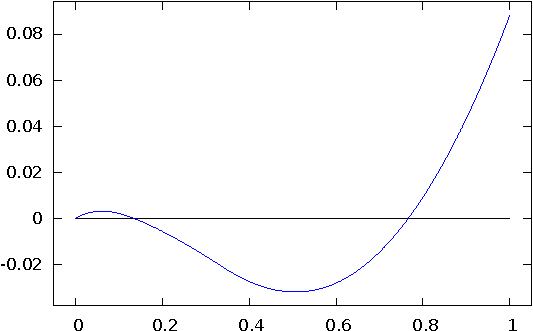
\includegraphics{figures/calculus_derivatives3},
\par\end{center}

\noindent yang akan kita sebut $F$, dapat dengan mudah disangka sebagai
polinom kubik atau polinom berderajat lebih tinggi, padahal fungsi
ini sama sekali tidak sesederhana itu. Pertama, domainnya adalah interval
$[0,1]$, sehingga grafik yang ditampilkan merupakan keseluruhan grafiknya.
Kedua, fungsi ini hanya memiliki dua turunan. Ketiga, definisinya
agak tidak lazim. Kita akan segera membahasnya lebih lanjut.

Di sini kita berhadapan dengan antiturunan dari suatu fungsi interpolasi
fraktal. Fungsi interpolasi adalah fungsi yang grafiknya melalui sekumpulan
titik yang ditentukan. Fungsi ini kebetulan bersifat fraktal, sehingga
merupakan fungsi interpolasi \textit{fraktal}. Fungsi interpolasi
fraktal $f$ melalui
\begin{equation}
(0,.123),\ (.33,-.123),\mbox{ dan }(1,.5)\label{eq:interpolationPoints}
\end{equation}
sedemikian rupa sehingga grafik yang ditampilkan adalah grafik antiturunannya.
Ketidaklaziman definisi $F$ berasal dari ketidaklaziman definisi
$f$:
\[
f(x)=\begin{cases}
f_{1}+c_{1}\frac{x}{\alpha}+d_{1}f\left(\frac{x}{\alpha}\right), & 0\leq x\leq\alpha\\
f_{2}+c_{2}\frac{x-\alpha}{1-\alpha}+d_{2}f\left(\frac{x-\alpha}{1-\alpha}\right), & \alpha\leq x\leq1
\end{cases}
\]
dengan
\[
\begin{gathered}f_{1}=\frac{8979}{100000},\ c_{1}=-\frac{34779}{100000},\ d_{1}=\frac{27}{100}\\
f_{2}=-\frac{75891}{550000},\ c_{2}=\frac{317391}{550000},\ d_{2}=\frac{67}{550}\\
\alpha=\frac{33}{100}.
\end{gathered}
\]

\noindent\begin{digression}{Fungsi Interpolasi Fraktal}

\noindent Fungsi interpolasi fraktal dapat melalui lebih dari tiga
titik. Bahkan, tiga merupakan jumlah minimum titiknya. Secara umum,
untuk $n\geq3$, andaikan $x_{1}<x_{2}<\cdots<x_{n}$. Fungsi interpolasi
fraktal linear (terdapat jenis fungsi interpolasi fraktal lainnya)
yang melalui setiap titik
\[
(x_{1},y_{1}),(x_{2},y_{2}),\ldots,(x_{n},y_{n})
\]
dan berdomain $[x_{1},x_{n}]$ didefinisikan oleh transformasi linear
\[
L_{i}\left(\begin{array}{c}
x\\
y
\end{array}\right)=\left(\begin{array}{cc}
a_{i} & 0\\
c_{i} & d_{i}
\end{array}\right)\left(\begin{array}{c}
x\\
y
\end{array}\right)+\left(\begin{array}{c}
e_{i}\\
f_{i}
\end{array}\right),\quad i=1,2,\ldots,n-1.
\]
Parameter $a_{i}$, $c_{i}$, $e_{i}$, serta $f_{i}$ dihitung berdasarkan
syarat bahwa fungsi tersebut menginterpolasi titik-titik yang diberikan.
Secara khusus, kita mensyaratkan
\[
L_{i}\left(\begin{array}{c}
x_{1}\\
y_{1}
\end{array}\right)=\left(\begin{array}{c}
x_{i}\\
y_{i}
\end{array}\right)\mbox{ dan }L_{i}\left(\begin{array}{c}
x_{n}\\
y_{n}
\end{array}\right)=\left(\begin{array}{c}
x_{i+1}\\
y_{i+1}
\end{array}\right).
\]
Parameter $d_{i}$ adalah parameter bebas dengan pembatasan $|d_{i}|<1$.
Dengan perhitungan aljabar langsung dapat ditunjukkan bahwa
\begin{eqnarray*}
a_{i} & = & \frac{x_{i+1}-x_{i}}{x_{n}-x_{1}}\\
c_{i} & = & \frac{y_{i+1}-y_{i}-d_{i}(y_{n}-y_{1})}{x_{n}-x_{1}}\\
e_{i} & = & x_{i}-a_{i}x_{1}\\
f_{i} & = & y_{i}-c_{i}x_{1}-d_{i}y_{1}.
\end{eqnarray*}

Secara bersama-sama, transformasi $L_{i}$ mendefinisikan fungsi $f$,
dengan setiap $L_{i}$ menangani subselang $[x_{i},x_{i+1}]$ dari
domain tersebut. $L_{i}\left(\begin{array}{c}
x\\
y
\end{array}\right)=\left(\begin{array}{c}
a_{i}x+e_{i}\\
c_{i}x+d_{i}y+f_{i}
\end{array}\right)$, sehingga ketika $L_{i}$ memetakan $x$ ke $a_{i}x+e_{i}$, transformasi
tersebut secara bersamaan memetakan $y$ ke $c_{i}x+d_{i}y+f_{i}$.
Karena $L_{i}$ menerapkan pemetaan ini pada fungsi $f$, harus berlaku
$f(a_{i}x+e_{i})=c_{i}x+d_{i}f(x)+f_{i}$ pada $[x_{1},x_{n}]$, atau
secara ekuivalen,
\[
f(x)=f_{i}+c_{i}\left(\frac{x-e_{i}}{a_{i}}\right)+d_{i}f\left(\frac{x-e_{i}}{a_{i}}\right)\mbox{ pada }[x_{i},x_{i+1}].
\]
Dengan menyatukan seluruh bagian tersebut, $f$ didefinisikan oleh
\[
f(x)=\begin{cases}
h_{1}(x), & x_{1}\leq x\leq x_{2}\\
h_{2}(x), & x_{2}\leq x\leq x_{3}\\
 & \vdots\\
h_{n-1}(x), & x_{n-1}\leq x\leq x_{n}
\end{cases}
\]
dengan
\[
h_{i}(x)=f_{i}+c_{i}\left(\frac{x-e_{i}}{a_{i}}\right)+d_{i}f\left(\frac{x-e_{i}}{a_{i}}\right).
\]
Akibatnya, $F(x)=\int_{x_{1}}^{x}f(t)\,dt$ didefinisikan oleh
\[
F(x)=\begin{cases}
\int_{x_{1}}^{x}h_{1}(t)dt, & x_{1}\leq x\leq x_{2}\\
F(x_{2})+\int_{x_{2}}^{x}h_{2}(t)dt, & x_{2}\leq x\leq x_{3}\\
 & \vdots\\
F(x_{n-1})+\int_{x_{n-1}}^{x}h_{n-1}(t)dt, & x_{n-1}\leq x\leq x_{n}
\end{cases}
\]
tanpa syarat tambahan, sedangkan $f'(x)$ didefinisikan oleh
\[
f'(x)=\begin{cases}
h_{1}'(x), & x_{1}\leq x\leq x_{2}\\
h_{2}'(x), & x_{2}<x\leq x_{3}\\
 & \vdots\\
h_{n-1}'(x), & x_{n-1}<x\leq x_{n}
\end{cases}
\]
asalkan $f'$ ada! Jika $\left|\frac{d_{i}}{a_{i}}\right|<1$ untuk
setiap $i$, maka turunannya ada hampir di mana-mana, tetapi pada
umumnya tidak kontinu. Jika selain itu berlaku $h_{i}'(x_{i+1})=h_{i+1}'(x_{i+1})$
untuk setiap $i=1,2,\ldots,n-2$, maka turunannya ada dan kontinu.
\begin{description}
\item [{Rujukan}] \cite[Bab 6]{barnsley}
\end{description}
\noindent\end{digression}

\noindent Definisi $f$ merujuk pada dirinya sendiri. Nilai-nilainya
didefinisikan, antara lain, melalui nilai-nilai fungsi itu sendiri!
Karena itu, penghitungan nilai fungsi ini agak berbeda dari penghitungan
nilai fungsi biasa. Sebagai contoh, karena $f$ melalui titik-titik
\ref{eq:interpolationPoints}, harus berlaku $f(0)=.123$, $f(.33)=-.123$,
dan $f(1)=.5$, yang dapat kita periksa dengan cukup mudah. Menurut
definisi,
\[
f(0)=f_{1}+d_{1}f(0)=.08979+.27f(0)
\]
 sehingga $f(0)$ didefinisikan sebagian oleh nilainya sendiri. Kita
perlu menyelesaikan persamaan $f(0)=.08979+.27f(0)$ untuk memperoleh
$f(0)$. Dengan demikian, kita memperoleh $f(0)=\frac{.08979}{.73}=.123$,
seperti yang dijanjikan. Sekali lagi menurut definisi, 
\[
f(1)=f_{2}+c_{2}+d_{2}f(1)=-\frac{75891}{550000}+\frac{317391}{550000}+\frac{67}{550}f(1).
\]
Dengan menyelesaikan persamaan tersebut terhadap $f(1)$, kita memperoleh
$f(1)=\frac{-\frac{75891}{550000}+\frac{317391}{550000}}{1-\frac{67}{550}}=\frac{1}{2}$,
seperti yang dijanjikan. Karena $\alpha=.33$, definisi tersebut sebenarnya
memberikan dua cara untuk menghitung $f(.33)$. Menurut bagian pertama
definisi $f$,
\begin{eqnarray*}
f(.33)=f(\alpha) & = & f_{1}+c_{1}+d_{1}f(1)\\
 & = & \frac{8979}{100000}-\frac{34779}{100000}+\frac{27}{100}\cdot\frac{1}{2}\\
 & = & -.123.
\end{eqnarray*}
Sekarang adalah saat yang tepat untuk memverifikasi bahwa $f(\alpha)=-.123$
juga berlaku menurut bagian kedua definisi $f$. Cobalah! Menghitung
nilai-nilai lain dari $f$ mungkin sedikit lebih menantang, tetapi
beberapa di antaranya masih cukup mudah. $\alpha^{2}<\alpha$ dan
$\alpha+(1-\alpha)\alpha>\alpha$, sehingga
\begin{eqnarray*}
f(\alpha^{2}) & = & f_{1}+c_{1}\alpha+d_{1}f\left(\alpha\right)\\
 & = & \frac{8979}{100000}-\frac{34779}{100000}\cdot\frac{33}{100}+\frac{27}{100}\cdot\left(-\frac{123}{1000}\right)\\
 & = & -.0581907\\
f(\alpha+(1-\alpha)\alpha) & = & f_{2}+c_{2}\alpha+d_{2}f\left(\alpha\right)\\
 & = & -\frac{75891}{550000}+\frac{317391}{550000}\cdot\frac{33}{100}+\frac{67}{550}\cdot\left(-\frac{123}{1000}\right)\\
 & = & \frac{2060703}{55000000}\\
 & = & .0374673\overline{27}
\end{eqnarray*}
Dengan tingkat kesulitan yang serupa, sekarang Anda dapat menghitung
\[
\begin{gathered}f(\alpha^{3}),\ f(\alpha(\alpha+(1-\alpha)\alpha)),\ f(\alpha+(1-\alpha)\alpha^{2}),\\
\mbox{dan }f(\alpha+(1-\alpha)(\alpha+(1-\alpha)\alpha)).
\end{gathered}
\]
Jawaban \vpageref{ans:evaluatingf}. Secara lebih umum, setelah Anda
menghitung $f(x)$ untuk suatu nilai $x$, Anda kemudian dapat menghitung
$f(\alpha x)$ dan $f(\alpha+(1-\alpha)x)$ dari nilai tersebut.

Setelah memahami $f$, kita mendefinisikan $F$ dengan $F(x)=\int_{0}^{x}f(t)\,dt$
untuk setiap $x\in[0,1]$. Dengan mengintegralkan $f(x)$, kita memperoleh
\[
F(x)=\begin{cases}
f_{1}x+\frac{c_{1}x^{2}}{2\alpha}+\alpha d_{1}F\left(\frac{x}{\alpha}\right), & 0\leq x\leq\alpha\\
F(\alpha)+f_{2}\left(x-\alpha\right)+\frac{c_{2}\left(x-\alpha\right)^{2}}{2(1-\alpha)}+(1-\alpha)d_{2}F\left(\frac{x-\alpha}{1-\alpha}\right), & \alpha\leq x\leq1
\end{cases}
\]
dengan kedua rumus tersebut sekali lagi berlaku ketika $x=\alpha$.
Sama seperti $f$, fungsi $F$ merujuk pada dirinya sendiri. Untuk
mencari nilai-nilai $F$, kita harus menjalani proses yang sama seperti
ketika mencari nilai-nilai $f$. Sebagai permulaan, $F(0)=\alpha d_{1}F(0)\Rightarrow(1-\alpha d_{1})\cdot F(0)=0,$
tetapi $\alpha$ dan $d_{1}$ keduanya kurang dari 1, sehingga $1-\alpha d_{1}\neq0$.
Oleh karena itu,
\[
F(0)=\frac{0}{1-\alpha d_{1}}=0.
\]
Nilai ini juga dapat kita hitung melalui integrasi: $F(0)=\int_{0}^{0}f(t)\,dt=0$.
Selanjutnya, menurut rumus tersebut,
\[
\begin{gathered}F(1)=F(\alpha)+(1-\alpha)\left(f_{2}+\frac{c_{2}}{2}+d_{2}F(1)\right)\\
\mbox{dan}\\
F(\alpha)=\alpha\left(f_{1}+\frac{c_{1}}{2}+d_{1}F(1)\right),
\end{gathered}
\]
yang merupakan sistem dua persamaan dengan dua peubah yang tidak diketahui,
yaitu $F(\alpha)$ dan $F(1)$. Solusinya adalah
\[
\begin{gathered}F(\alpha)=-\frac{121012947}{6081400000}\approx-.01989886325517151\\
F(1)=\frac{5361861}{60814000}\approx0.0881682014009932.
\end{gathered}
\]
Setelah memperoleh ketiga nilai $F(0),\ F(\alpha),$ dan $F(1)$,
kita dapat menghitung nilai-nilai lainnya seperti sebelumnya. Kedua
nilai $F(\alpha x)$ dan $F(\alpha+(1-\alpha)x)$ sama-sama bergantung
pada nilai $F(x)$. Jadi, kita dapat menghitung $F(\alpha^{2})$ dan
$F(\alpha+(1-\alpha)\alpha)$: 
\begin{eqnarray*}
F(\alpha^{2}) & = & f_{1}\alpha^{2}+\frac{c_{1}\alpha^{3}}{2}+\alpha d_{1}F\left(\alpha\right)\\
 & = & \frac{10678194456039}{6081400000000000}\\
 & \approx & .001755877668964219\\
F(\alpha+(1-\alpha)\alpha) & = & F(\alpha)+f_{2}\left(1-\alpha\right)\alpha+\frac{c_{2}\left(1-\alpha\right)\alpha^{2}}{2}+(1-\alpha)d_{2}F\left(\alpha\right)\\
 & = & -\frac{94196657189979}{3040700000000000}\\
 & \approx & -.03097860926430723.
\end{eqnarray*}
Sekarang Anda dapat menghitung sendiri $F(\alpha^{3})$, $F(\alpha(\alpha+(1-\alpha)\alpha))$,
$F(\alpha+(1-\alpha)\alpha^{2})$, serta $F(\alpha+(1-\alpha)(\alpha+(1-\alpha)\alpha))$.
Jawaban \vpageref{ans:evaluatingF}. Anda tidak perlu bersusah payah
menghitung nilai-nilai ini secara eksak. Hal itu memerlukan sistem
aljabar komputer dengan presisi arbitrer dan bukan merupakan tujuan
sebenarnya. Tujuannya adalah memastikan bahwa Anda memahami cara melakukan
perhitungannya. Gunakan kalkulator atau Octave beserta nilai-nilai
hampiran yang telah dihitung.

\subsection{Turunan $f$ dan grafik lainnya}

Fungsi $f$ memiliki turunan yang kontinu. Bahkan, parameter-parameter
yang mendefinisikan $f$ dipilih secara khusus agar turunannya ada
dan kontinu. Dengan menurunkan $f$, kita memperoleh
\[
f'(x)=\begin{cases}
\frac{c_{1}}{\alpha}+\frac{d_{1}}{\alpha}f'\left(\frac{x}{\alpha}\right), & 0\leq x\leq\alpha\\
\frac{c_{2}}{1-\alpha}+\frac{d_{2}}{1-\alpha}f'\left(\frac{x-\alpha}{1-\alpha}\right), & \alpha\leq x\leq1
\end{cases}
\]
 dan seperti sebelumnya, kita dapat memeriksa bahwa definisi tersebut
konsisten ketika $x=\alpha$:
\[
\begin{gathered}f'(0)=\frac{c_{1}}{\alpha}+\frac{d_{1}}{\alpha}f'(0)\Rightarrow f'(0)=\frac{c_{1}}{\alpha-d_{1}}=-\frac{11593}{2000}=\text{\textminus}5.7965\\
f'(1)=\frac{c_{2}}{1-\alpha}+\frac{d_{2}}{1-\alpha}f'(1)\Rightarrow f'(1)=\frac{c_{2}}{1-\alpha-d_{2}}=\frac{105797}{100500}\approx1.052706467661692\\
f'(\alpha)=\frac{c_{1}}{\alpha}+\frac{d_{1}}{\alpha}f'(1)=-\frac{141949}{737000}\approx-.1926037991858887\\
f'(\alpha)=\frac{c_{2}}{1-\alpha}+\frac{d_{2}}{1-\alpha}f'(0)=-\frac{141949}{737000}\approx-.1926037991858887.
\end{gathered}
\]
Nilai-nilai lain dari $f'$ dapat dihitung dengan cara yang digunakan
untuk $f$ dan $F$. Grafik $f$ dan $f'$ ditampilkan pada Gambar
\ref{fig:Graphf} dan \ref{fig:Graphfprime}. 
\begin{figure}

\caption{\label{fig:Graphf}Grafik $f$.}

\centering{}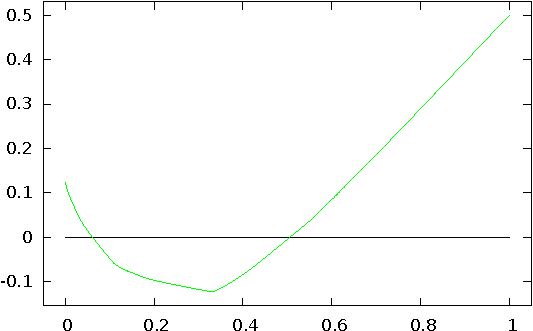
\includegraphics{figures/calculus_derivatives2}
\end{figure}
 
\begin{figure}

\caption{\label{fig:Graphfprime}Grafik $f'$.}

\begin{centering}
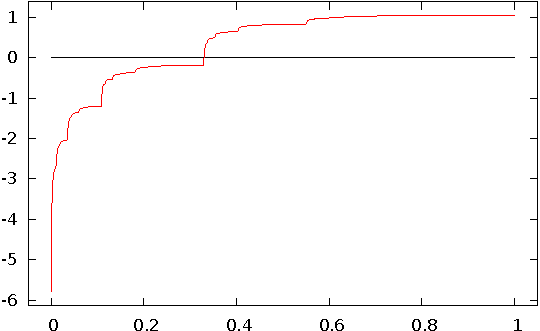
\includegraphics{figures/calculus_derivatives1}
\par\end{centering}
\end{figure}

Demikianlah pembahasannya. Sekarang, cobalah mencari akar ketiga fungsi
tersebut. Kode Octave berikut akan membantu Anda mengevaluasi fungsi-fungsi
itu pada titik mana pun dan sangat menghemat waktu!

\subsection{Octave}

\begin{verbatim}
%%%%%%%%%%%%%%%%%%%%%%%%%%%%%%%%%%%%%%%%%%%%%%%%%%%%%%%%%%
% Written by Dr. Len Brin               19 February 2014 %
% Purpose: Calculate values of the fractal interpolating %
%        function, f, passing through                    %
%        (0,f_0), (alpha,f_alpha), and (1,f_1),          %
%        its derivative and its integral.                %
% INPUT: value at which to evaluate, x; array of values, %
%        f = [f_0,f_alpha,f_1]; alpha; scaling factors   %
%        d1 and d2.                                      %
% OUTPUT: y=f'(x); yy=f(x); yyy=F(x).                    %
%%%%%%%%%%%%%%%%%%%%%%%%%%%%%%%%%%%%%%%%%%%%%%%%%%%%%%%%%%
function [y,yy,yyy] = fractalInterpolator(x,f,alpha,d1,d2)
  f1=f(1)*(1-d1);
  c1=f(2)-d1*f(3)-f1;
  f2=f(2)-d2*f(1);
  c2=(1-d2)*f(3)-f2;
  F1=(alpha*(f1+c1/2)+(1-alpha)*(f2+c2/2))/(1-(1-alpha)*d2-alpha*d1);
  FA=alpha*(f1+c1/2+d1*F1);
  l=0;
  r=1;
  a=[];
  if (alpha>1/2)
    its=floor(log(10^-16)/log(alpha));
  else
    its=floor(log(10^-16)/log(1-alpha));
  end%if
  for i=1:its
    if (alpha>1/2)
      h = (r-l)*alpha;
      m = l+h;
    else
      h = (r-l)*(1-alpha);
      m = r-h;
    end%if
    if (x<m)
      a(i)=0;
      r=m;
    else
      a(i)=1;
      l=m;
    end%if
  end%for
  x=0;
  y=c1/(alpha-d1);
  yy=f(1);
  yyy=0;
  for i=its:-1:1
    if (a(i)==0)
      y=(c1+d1*y)/alpha;
      yy=c1*x+d1*yy+f1;
      yyy=alpha*(f1*x+c1/2*x*x+d1*yyy);
      x=alpha*x;
    else
      y=(c2+d2*y)/(1-alpha);
      yy=c2*x+d2*yy+f2;
      yyy=FA+(1-alpha)*(f2*x+c2/2*x*x+d2*yyy);
      x=alpha+(1-alpha)*x;
    end%if
  end%for
end%function 
\end{verbatim}\texttt{fractalInterpolator.m} dapat diunduh dari \href{http://lqbrin.github.io/tea-time-numerical/ancillaries.html}{situs pendamping}.

\subsection*{Jawaban}
\begin{description}
\item [{Menghitung}] nilai~$f$: \label{ans:evaluatingf}Berikut adalah
beberapa nilai $f$:
\begin{eqnarray*}
f(\alpha^{3}) & \approx & .03620418000000000\\
f(\alpha(\alpha+(1-\alpha)\alpha)) & \approx & -.09176089063636364\\
f(\alpha+(1-\alpha)\alpha^{2}) & \approx & -.08222890363636364\\
f(\alpha+(1-\alpha)(\alpha+(1-\alpha)\alpha)) & \approx & .1846063473223140.
\end{eqnarray*}
\item [{Menghitung}] nilai~$F$: \label{ans:evaluatingF}Berikut adalah
beberapa nilai $F$:
\begin{eqnarray*}
F(\alpha^{3}) & \approx & .002702687013731212\\
F(\alpha(\alpha+(1-\alpha)\alpha)) & \approx & -.003859289400223274\\
F(\alpha+(1-\alpha)\alpha^{2}) & \approx & -.02753062961856850\\
F(\alpha+(1-\alpha)(\alpha+(1-\alpha)\alpha)) & \approx & -.01466250212441314.
\end{eqnarray*}
\end{description}




\section{\label{sec:polynomialLagrange}Polinom Lagrange}

Suatu fungsi yang grafiknya harus melalui sekumpulan titik yang ditentukan
disebut fungsi interpolasi\index{fungsi interpolasi}, dan kita mengatakan
bahwa fungsi tersebut menginterpolasi titik-titik yang ditentukan.
Selanjutnya, proses mencari fungsi semacam itu disebut interpolasi. 

Pada latihan \ref{polynomials}a di bagian \ref{sec:moreConvergenceDiagrams},
Anda diminta mencari polinom yang berakar di $-7,2$, dan $1\pm5i$
(dan tidak memiliki akar lain). Oleh karena itu, fungsi tersebut harus
berupa polinom dan grafiknya harus melalui titik-titik 
\begin{equation}
(-7,0),\ (2,0),\ (1+5i,0),\mbox{ dan }(1-5i,0).\label{eq:interpolationExample}
\end{equation}
Jika ditinjau kembali, pertanyaan itu dapat dirumuskan sebagai berikut:
carilah polinom yang melalui titik-titik \ref{eq:interpolationExample}
(dan tidak memiliki akar selain $-7$, $2$, $1+5i$, dan $1-5i$);
ini merupakan masalah interpolasi. Sekarang kita memperluas gagasan
ini dengan meninjau polinom yang grafiknya melalui titik-titik dengan
ordinat sembarang (bukan hanya $0$).

Kita mulai dari hal yang sudah dikenal. Polinom $p(x)=(x+7)(x-2)$
berakar di $-7$ dan $2$ sehingga grafiknya melalui $(-7,0)$ dan
$(2,0)$. Misalkan kita ingin mengubah $p$ agar grafiknya juga melalui
$(-1,1)$. Artinya, kita menginginkan $p(-7)=0$, $p(-1)=1$, dan
$p(2)=0$. Berangkat dari $p(x)=(x+7)(x-2)$, kita sudah mempunyai
$p(-7)=0$ dan $p(2)=0$, sehingga sebenarnya kita hanya perlu memusatkan
perhatian pada $p(-1)=1$. Dalam bentuknya sekarang, $p(-1)=(-1+7)(-1-2)=6(-3)=-18$,
sangat jauh dari $1$. Namun, $p(x)=(x+7)(x-2)$ bukan satu-satunya
polinom yang melalui $(-7,0)$ dan $(2,0)$. Ambil $a$ sembarang
bilangan real dan perhatikan bahwa $q(x)=a(x+7)(x-2)$ juga melalui
$(-7,0)$ dan $(2,0)$. Jika kita memilih $a$ sedemikian rupa sehingga
$q(-1)=1$, kita memperoleh fungsi yang diinginkan:
\[
q(-1)=a(-1+7)(-1-2)=-18a=1\Rightarrow a=-\frac{1}{18}.
\]
 $q(x)=-\frac{1}{18}(x+7)(x-2)$ melalui ketiga titik tersebut, yaitu
$(-7,0)$, $(2,0)$, dan $(-1,1)$. Namun, jangan sampai kita kehilangan
jejak asal konstruksi ini. $-\frac{1}{18}=\frac{1}{p(-1)}$, sehingga
sebenarnya fungsi yang diinginkan dapat ditulis sebagai $q(x)=\frac{p(x)}{p(-1)}$.
Memang, $q(-7)=\frac{p(-7)}{p(-1)}=0$, $q(2)=\frac{p(2)}{p(-1)}=0$,
dan $q(-1)=\frac{p(-1)}{p(-1)}=1$. 

Sekarang misalkan kita menginginkan polinom yang melalui $(-7,0)$,
$(2,0)$, dan $(-1,\sqrt{2})$. Seperti sebelumnya, kita mengetahui
bahwa $p(x)=(x+7)(x-2)$ mempunyai akar yang diinginkan dan $q(x)=\frac{p(x)}{p(-1)}$
memiliki sifat yang berguna, yaitu $q(-1)=1$. Kita menggunakan kedua
fakta ini untuk memperoleh jawaban. Bahkan, tanpa melakukan perhitungan
apa pun, kita mengetahui bahwa polinom 
\[
l(x)=\frac{p(x)}{p(-1)}\sqrt{2}
\]
adalah fungsi yang diinginkan. Luangkan waktu sejenak untuk memeriksa
bahwa $l(-7)=0$, $l(2)=0$, dan $l(-1)=\sqrt{2}$, dan memahami konstruksinya.
Gagasan ini merupakan benih dari apa yang disebut bentuk Lagrange
bagi polinom interpolasi.

Kini kita siap membiarkan ordinatnya sembarang! Misalkan kita menginginkan
polinom yang melalui $(-7,y_{1}),$ $(2,y_{2})$, dan $(-1,y_{3})$.
Kita mengetahui bahwa polinom $p_{3}(x)=(x+7)(x-2)$ berakar di $-7$
dan $2$, sehingga polinom $l_{3}(x)=\frac{p_{3}(x)}{p_{3}(-1)}y_{3}$
bernilai nol di $-7$ dan $2$, sedangkan $l_{3}(-1)=y_{3}$. Ini
merupakan langkah pertama yang baik. Polinom ini menghasilkan ordinat
yang tepat pada $-1$ dan bernilai nol di $-7$ dan $2$. Dengan cara
serupa, kita dapat mengonstruksi polinom $p_{2}(x)=(x+7)(x+1)$ yang
berakar di $-7$ dan $-1$; dari polinom ini kita dapat mengonstruksi
polinom $l_{2}(x)=\frac{p_{2}(x)}{p_{2}(2)}y_{2}$ yang bernilai nol
di $-7$ dan $-1$, sedangkan $l_{2}(2)=y_{2}$. Ini merupakan langkah
kedua yang baik. Polinom ini menghasilkan ordinat yang tepat pada
$2$ dan bernilai nol di $-7$ dan $-1$. Sekarang tinjau jumlah $(l_{3}+l_{2})$.
$l_{3}(-1)=y_{3}$ dan $l_{2}(-1)=0$, sehingga $(l_{3}+l_{2})(-1)=y_{3}$.
Dengan cara serupa, $l_{3}(2)=0$ dan $l_{2}(2)=y_{2}$, sehingga
$(l_{3}+l_{2})(2)=y_{2}$. Selain itu, $(l_{3}+l_{2})(-7)=0$. Kini
kita mempunyai polinom yang melalui dua dari tiga titik yang disyaratkan
dan bernilai nol pada absis titik ketiga. Jika kita mempunyai polinom
yang menghasilkan ordinat yang tepat pada $-7$ dan bernilai nol di
$2$ dan $-1$, kita dapat menambahkannya ke jumlah tersebut dan menyelesaikan
konstruksi. Namun, justru polinom seperti inilah yang telah kita konstruksikan!
Kita menetapkan $p_{1}(x)=(x+1)(x-2)$ dan $l_{1}(x)=\frac{p_{1}(x)}{p_{1}(-7)}y_{1}$,
lalu memperhatikan bahwa $l_{1}$ menghasilkan ordinat yang tepat
pada $-7$ dan bernilai nol di $2$ dan $-1$, tepat seperti yang
kita perlukan. Akhirnya, polinom yang diinginkan adalah $(l_{1}+l_{2}+l_{3})$.
Tabel \ref{tab:interpolationExample} 
\begin{table}
\hrule \caption{\label{tab:interpolationExample}Polinom yang melalui $(-7,y_{1})$,
$(2,y_{2})$, dan $(-1,y_{3})$.}

\centering{}\medskip{}
\begin{tabular}{c|ccc|c}
$x$ & $l_{1}(x)=\frac{p_{1}(x)}{p_{1}(-7)}y_{1}$ & $l_{2}(x)=\frac{p_{2}(x)}{p_{2}(2)}y_{2}$ & $l_{3}(x)=\frac{p_{3}(x)}{p_{3}(-1)}y_{3}$ & $(l_{1}+l_{2}+l_{3})(x)$\tabularnewline
\hline 
$-7$ & $y_{1}$ & $0$ & $0$ & $y_{1}$\tabularnewline
$2$ & $0$ & $y_{2}$ & $0$ & $y_{2}$\tabularnewline
$-1$ & $0$ & $0$ & $y_{3}$ & $y_{3}$\tabularnewline
\end{tabular}\medskip{}
\hrule 
\end{table}
merangkum konstruksi tersebut.

Sekarang kita siap melakukan generalisasi sepenuhnya. Misalkan $n\geq1$
dan $x_{0},x_{1},\ldots,x_{n}$ adalah $n$ bilangan real yang berbeda.
Kita menggunakan notasi $P_{n}(x)$ untuk polinom berderajat terendah
yang menginterpolasi titik-titik
\[
(x_{0},y_{0}),(x_{1},y_{1}),\ldots,(x_{n},y_{n}).
\]

Dengan menetapkan ${\displaystyle p_{i}(x)=\prod_{\substack{j=0\\
j\neq i
}
}^{n}(x-x_{j})=(x-x_{0})\cdots(x-x_{i-1})(x-x_{i+1})\cdots(x-x_{n})}$, salah satu rumus untuk $P_{n}$ adalah 
\begin{equation}
L_{n}(x)=\sum_{i=0}^{n}\frac{p_{i}(x)}{p_{i}(x_{i})}y_{i}.\label{eq:lagrangeInterpolatingPolynomial}
\end{equation}
Dalam bentuk ini, $L_{n}$ disebut \textit{bentuk Lagrange}\index{bentuk Lagrange}
dari $P_{n}$. Demi keringkasan, bentuk ini sering disebut polinom
interpolasi Lagrange, atau bahkan polinom Lagrange. Namun, apa pun
namanya, polinom interpolasi berderajat terendah itu tetaplah $P_{n}$.
Kita akan tetap menyebutnya polinom interpolasi berderajat terendah,
atau menggunakan notasi $P_{n}$, jika bentuknya tidak penting; dan
kita akan menambahkan frasa \textit{bentuk Lagrange}, atau menggunakan
notasi $L_{n}$, jika bentuknya penting.

Penggunaan utama polinom interpolasi dalam analisis numerik adalah
untuk menghampiri fungsi nonpolinom dengan cara berikut. Misalkan
kita mengetahui nilai $f$ pada beberapa titik. Artinya, kita mengetahui
$f(x_{0})=y_{0},f(x_{1})=x_{1},\ldots,f(x_{n})=y_{n}$ dan mungkin
tidak mengetahui banyak hal lainnya. Berdasarkan konstruksinya, polinom
interpolasi berderajat terendah yang melalui $n+1$ titik
\[
(x_{0},y_{0}),(x_{1},y_{1}),\ldots,(x_{n},y_{n})
\]
akan sama dengan $f$ pada $x_{0},x_{1},\ldots,x_{n}$ dan kita dapat
menyatakan dengan cukup tepat seberapa dekat polinom interpolasi ini
dengan $f$ pada titik-titik lain. Nilai polinom interpolasi pada
``titik-titik lain'' inilah yang kita sebut hampiran terhadap fungsi
nonpolinom.

Dengan menetapkan $a=\min(x_{0},\ldots,x_{n},x)$ dan $b=\max(x_{0},\ldots,x_{n},x)$,
kita memperoleh hasil berikut. Jika $f$ mempunyai $n+1$ turunan
pada $(a,b)$ dan $f,f',f'',\ldots,f^{(n)}$ semuanya kontinu pada
$[a,b]$, maka terdapat $\xi_{x}\in(a,b)$ sedemikian sehingga 
\begin{equation}
f(x)-P_{n}(x)=\frac{f^{(n+1)}(\xi_{x})}{(n+1)!}(x-x_{0})(x-x_{1})\cdots(x-x_{n}).\label{eq:lagrangeInterpolatingPolynomialError}
\end{equation}
Menariknya, hasil ini dibuktikan dengan meninjau bentuk Lagrange dari
suatu polinom interpolasi dalam variabel $t$ yang sama dengan galat
pada $x$ dan sama dengan nol pada setiap $x_{i}$. Polinom itu adalah
\[
\Lambda(t)=\left[P_{n}(x)-f(x)\right]\frac{(t-x_{0})(t-x_{1})\cdots(t-x_{n})}{(x-x_{0})(x-x_{1})\cdots(x-x_{n})}.
\]

\noindent\begin{digression}{$\Lambda$} 

\noindent$\Lambda$ adalah huruf kapital kesebelas dalam alfabet
Yunani dan dilafalkan  \texttt{\textbf{lam}}\texttt{-}\texttt{\textit{da}}.
Bentuk huruf kecilnya, $\lambda$, jauh lebih sering muncul dalam
matematika dan kerap menyatakan nilai eigen.

\noindent\end{digression} 

\noindent Dengan mengurangkan polinom ini dari galat, $e(t)=P_{n}(t)-f(t)$,
kita memperoleh fungsi
\[
g(t)=e(t)-\Lambda(t),
\]
yang bernilai nol untuk semua $t=x_{0},x_{1},\ldots,x_{n},x$. Karena
$g,g',\ldots,g^{(n)}$ semuanya kontinu pada $[a,b]$ dan $g^{(n+1)}$
ada pada $(a,b)$, berdasarkan Teorema Rolle yang Diperumum terdapat
$\xi_{x}\in(a,b)$ sedemikian sehingga $g^{(n+1)}(\xi_{x})=0$. Di
sisi lain, 
\begin{eqnarray*}
g^{(n+1)}(\xi_{x}) & = & e^{(n+1)}(\xi_{x})-\Lambda^{(n+1)}(\xi_{x})\\
 & = & P_{n}^{(n+1)}(\xi_{x})-f^{(n+1)}(\xi_{x})-\Lambda^{(n+1)}(\xi_{x}),
\end{eqnarray*}
dan $P_{n}$ merupakan polinom berderajat paling tinggi $n$. Oleh
karena itu, $P_{n}^{(n+1)}(t)=0$ untuk setiap $t$ dan kita memperoleh
$g^{(n+1)}(\xi_{x})=-f^{(n+1)}(\xi_{x})-\Lambda^{(n+1)}(\xi_{x})=0$.
Akibatnya, 
\[
f^{(n+1)}(\xi_{x})=-\Lambda^{(n+1)}(\xi_{x}).
\]
Namun, $\Lambda$ adalah polinom berderajat $n+1$ dalam $t$, sehingga
turunan ke-$(n+1)$ terhadap $t$ konstan terhadap $t$. Kita menuliskan
$\Lambda$ sebagai
\[
\Lambda(t)=\frac{P_{n}(x)-f(x)}{(x-x_{0})(x-x_{1})\cdots(x-x_{n})}\left[t^{n+1}+b_{n}t^{n}+\cdots+b_{0}t^{0}\right]
\]
untuk beberapa konstanta $b_{n},b_{n-1},\ldots,b_{0}$, dan akibatnya,
\[
\Lambda^{(n+1)}(t)=\frac{P_{n}(x)-f(x)}{(x-x_{0})(x-x_{1})\cdots(x-x_{n})}\cdot(n+1)!,
\]
dengan substitusi kita memperoleh
\[
f^{(n+1)}(\xi_{x})=\frac{f(x)-P_{n}(x)}{(x-x_{0})(x-x_{1})\cdots(x-x_{n})}\cdot(n+1)!
\]
atau, secara ekuivalen,
\[
\frac{f^{(n+1)}(\xi)}{(n+1)!}(x-x_{0})(x-x_{1})\cdots(x-x_{n})=f(x)-P_{n}(x)
\]
seperti yang hendak dibuktikan.

Gambar \ref{fig:Three-interpolating-functions.} 
\begin{figure}
\caption{\label{fig:Three-interpolating-functions.}Tiga fungsi yang diinterpolasi.
Dari atas ke bawah, $e^{\sin\left((x+1)^{2}\right)}$, $\sin\left(e^{(x+1)^{2}}\right)$,
dan fungsi fraktal sebagaimana didefinisikan pada bagian \ref{sec:rootFindingChallenge}.
$f$ ditampilkan dengan warna hitam, sedangkan interpolannya, $L_{6}$,
dengan warna merah.}

\centering{}%
\begin{tabular}{cc}
$f(x)$ dan $L_{6}(x)$ & $f^{(6)}(x)$\tabularnewline
\hline 
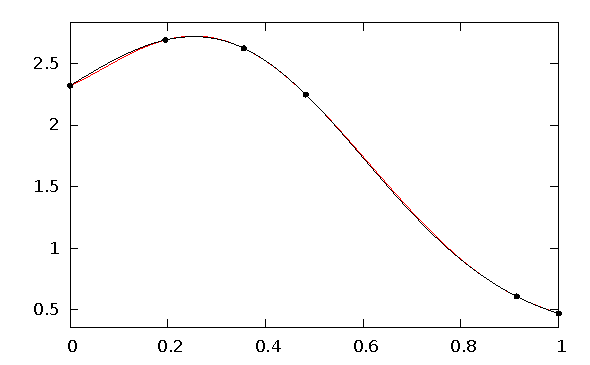
\includegraphics[scale=0.75]{figures/interpolation-polynomials1} & 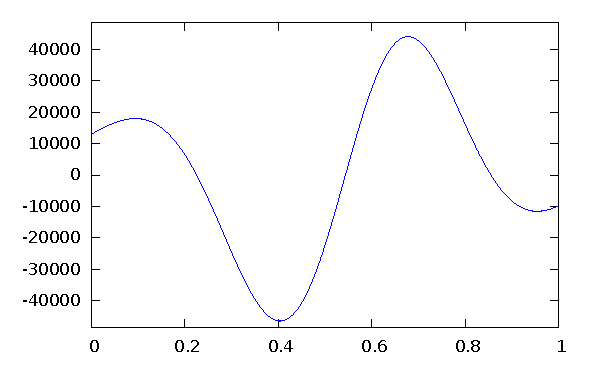
\includegraphics[scale=0.75]{figures/interpolation-polynomials2}\tabularnewline
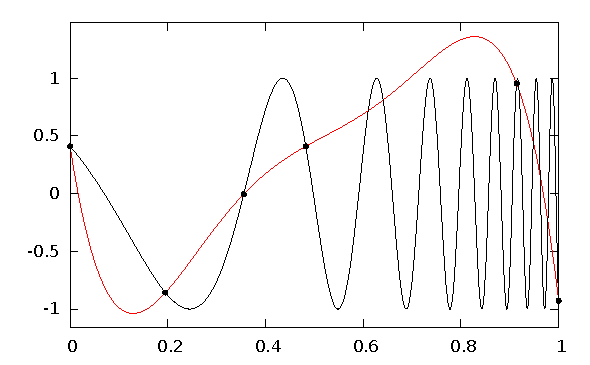
\includegraphics[scale=0.75]{figures/interpolation-polynomials3} & 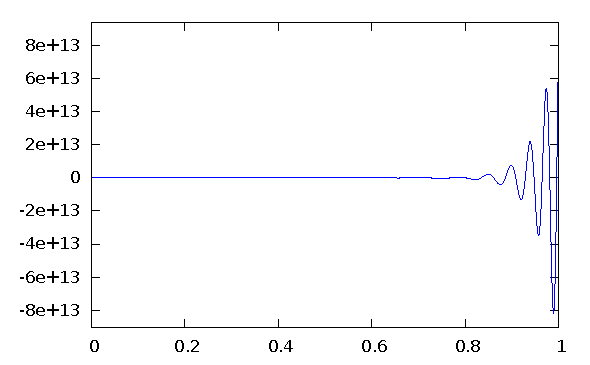
\includegraphics[scale=0.75]{figures/interpolation-polynomials4}\tabularnewline
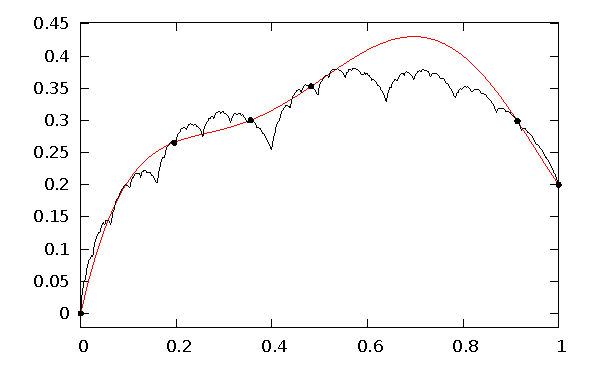
\includegraphics[scale=0.75]{figures/interpolation-polynomials5} & 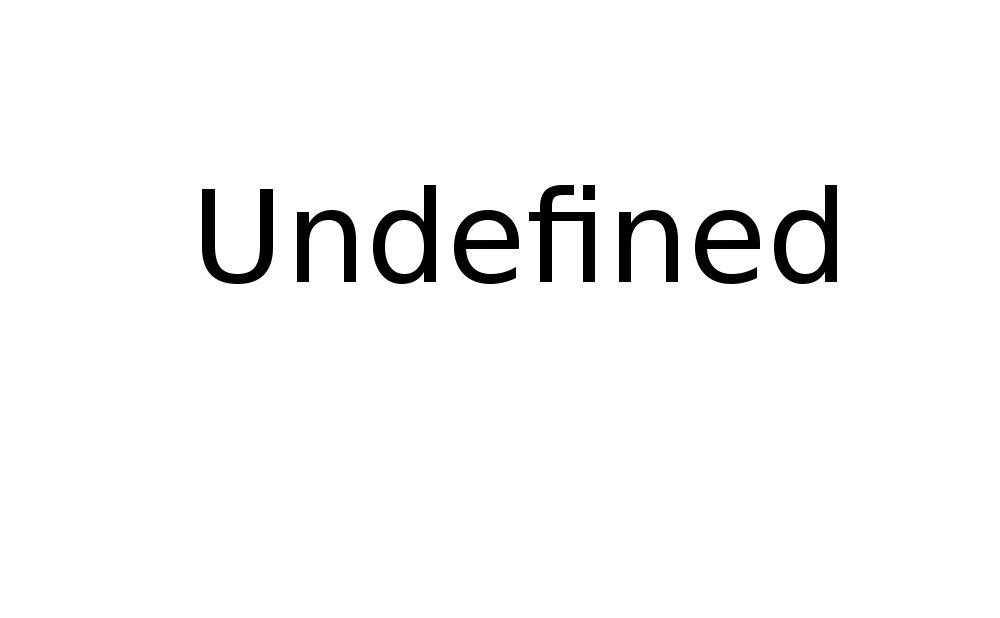
\includegraphics[scale=0.75]{figures/undefined}\tabularnewline
\end{tabular}
\end{figure}
 memperlihatkan polinom interpolasi untuk tiga fungsi yang berbeda.
Koordinat $x$ dari titik-titik yang ditentukan sama untuk setiap
polinom interpolasi. Koordinat $x$ tersebut adalah 
\[
0,.1951846177977887,.3554400571592862,.4823905248516196,.9138095996128959,\mbox{ dan }1.
\]
Empat bilangan di antara 0 dan 1 dipilih dengan generator bilangan
acak. Hanya pada kasus pertama polinom interpolasi sangat menyerupai
fungsinya. Turunan keenam $f$ membantu menjelaskan alasannya. 

Suku galat kita, 
\[
\frac{f^{(6)}(\xi)}{6!}(x-x_{0})(x-x_{1})\cdots(x-x_{5})
\]
menyiratkan bahwa turunan keenam $f$ dan polinom $h(x)=\frac{(x-x_{0})(x-x_{1})\cdots(x-x_{5})}{6!}$
menentukan seberapa besar perbedaan antara $f$ dan $L_{6}$. Dengan
membatasi $\left|f^{(6)}\right|$ dan $\left|h\right|$ pada selang
$[0,1]$, kita dapat memperoleh batas bagi selisih antara $f$ dan
$L_{6}$. Grafik $f^{(6)}$ ditampilkan pada Gambar \ref{fig:Three-interpolating-functions.}.
Grafik $h$ adalah

\begin{center}
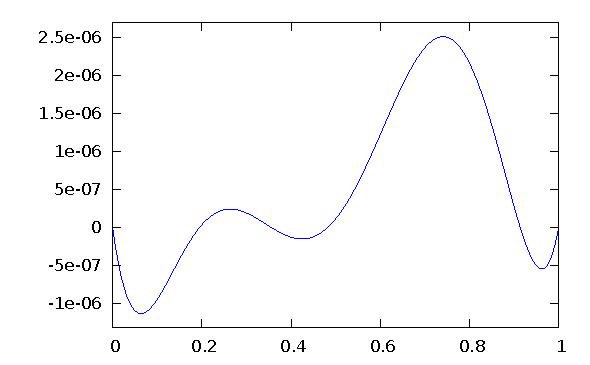
\includegraphics{figures/interpolation-polynomials6}
\par\end{center}

\noindent sehingga $\max_{x\in[0,1]}|h(x)|$ terjadi di sekitar $0.75$.
Kita dapat menerapkan metode pencarian akar pada $h'$ untuk menemukan
bahwa maksimum $|h|$ kira-kira $h(.7409254943919)\approx2.506891519629(10)^{-6}$,
suatu bilangan yang relatif kecil. Di sisi lain, untuk $f(x)=e^{\sin\left((x+1)^{2}\right)}$,
kita memperoleh $\max_{x\in[0,1]}\left|f^{(6)}(x)\right|\approx f^{(6)}(.6777170541644)\approx44013.74605321$,
suatu bilangan yang relatif besar. Hasil kali keduanya,
\[
\max_{x\in[0,1]}|h(x)|\cdot\max_{x\in[0,1]}\left|f^{(6)}(x)\right|\approx.11,
\]
memberikan batas galat. Jarak mutlak terbesar antara $L_{6}$ dan
$f$ pada selang $[0,1]$ tidak mungkin melebihi $0.11$, suatu bilangan
yang relatif kecil. Galat sebenarnya jauh lebih kecil sehingga hampir
tidak terlihat pada grafik kiri atas Gambar \ref{fig:Three-interpolating-functions.}.

Untuk $f(x)=\sin\left(e^{(x+1)^{2}}\right)$, kita memperoleh $\max_{x\in[0,1]}\left|f^{(6)}(x)\right|\approx f^{(6)}(1)\approx8.552147927657737(10)^{13}$,
suatu bilangan yang relatif besar. Kali ini hasil kalinya,
\[
\max_{x\in[0,1]}|h(x)|\cdot\max_{x\in[0,1]}\left|f^{(6)}(x)\right|\approx2.1439307114460004(10)^{8},
\]
merupakan bilangan yang sangat besar dibandingkan dengan nilai $f$.
Jadi, batas galat teoretis tidak meramalkan hasil yang baik bagi interpolasi
ini. Bahkan, batas itu menunjukkan bahwa interpolasinya dapat jauh,
jauh lebih buruk!$L_{6}$ mungkin berbeda dari $f$ sebesar lebih
dari dua juta; hal ini patut dikhawatirkan karena $f$ bernilai antara
$-1$ dan $1$. Hampiran yang meleset bahkan sebesar $1$ sama sekali
tidak berguna untuk fungsi $f$ ini. Dalam keadaan ini, kita tidak
perlu terkejut bahwa $L_{6}$ bukan hampiran yang baik terhadap $f$
karena suku galatnya dapat sangat besar. Meskipun demikian, metodenya
tetap sah. Kegagalan menghampiri $f$ dengan baik bukanlah kelemahan
metode, melainkan kekeliruan dalam penerapannya. Jika kita benar-benar
ingin menghampiri $f$ dengan baik, kita perlu memilih himpunan titik
interpolasi yang berbeda.

Untuk fungsi fraktal di kiri bawah Gambar \ref{fig:Three-interpolating-functions.},
taksiran galat kita sama sekali tidak relevan. Turunan keenam $f$
tidak ada. Bahkan, turunan pertama $f$ pun tidak ada. Kita tidak
dapat menaksir galat selain dengan melihat grafik. Dan seperti terlihat,
$L_{6}$ kembali menjadi hampiran yang sangat buruk terhadap $f$.
Sekali lagi, kegagalan itu bukanlah kelemahan metode, melainkan kekeliruan
penerapannya. Menghampiri fungsi dengan polinom interpolasi mengandaikan
bahwa fungsi tersebut mempunyai cukup banyak turunan.

\noindent\begin{digression}{Polinom Bernstein}\index{polinom Bernstein}

\noindent Misalkan $f$ adalah fungsi kontinu pada selang $[0,1]$,
dan definisikan polinom
\[
B_{n}(x)=\sum_{\nu=0}^{n}\begin{pmatrix}n\\
\nu
\end{pmatrix}f\left(\frac{\nu}{n}\right)x^{\nu}(1-x)^{n-\nu},\quad n=1,2,3,\ldots
\]
Maka 
\[
\lim_{n\to\infty}B_{n}(x)=f(x)
\]
secara seragam. Artinya, $\lim_{n\to\infty}\max\{|B_{n}(x)-f(x)|:x\in[0,1]\}=0$.
Polinom $B_{n}$ disebut polinom Bernstein. Di bawah ini ditampilkan
$B_{4}$, $B_{20}$, $B_{100}$, dan $B_{500}$ untuk fungsi fraktal
pada Gambar \ref{fig:Three-interpolating-functions.}.

\begin{center}
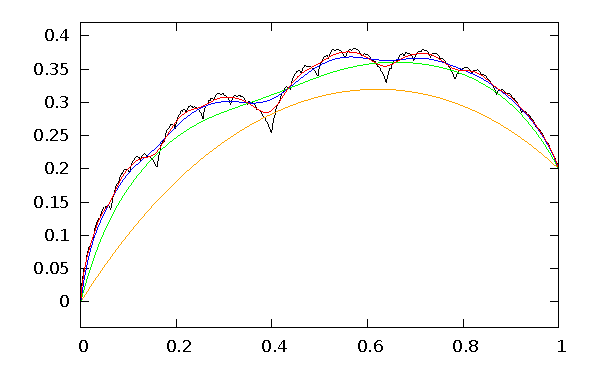
\includegraphics{figures/interpolation-polynomials7}
\par\end{center}

\noindent\end{digression}

\subsection{Penerapan polinom interpolasi}

Sekali lagi kita menghubungkan materi bab sebelumnya dengan bab ini.
Metode sekan sebenarnya merupakan penerapan polinom interpolasi pada
pencarian akar. Garis sekan yang kemiringannya digunakan untuk menghitung
suatu iterasi dapat dipandang sebagai garis interpolasi! Garis itu
melalui dua titik pada $g$. Karena itu, garis tersebut merupakan
hampiran terhadap $g$.

Dengan sudut pandang ini, kita dapat menggeneralisasi metode tersebut
dengan menggunakan turunan polinom interpolasi berderajat lebih tinggi
untuk menghampiri $g'$ pada setiap langkah. Metode umum ini, yang
akan kita sebut metode Sidi berderajat $k$ \cite{sidi},\index{metode Sidi}\index{metode!Sidi|see{metode Sidi}}
diringkas oleh rumus 
\[
x_{n+1}=x_{n}-\frac{g(x_{n})}{p'_{n,k}(x_{n})}
\]
 dengan $p_{n,k}$ sebagai polinom interpolasi yang melalui titik-titik
\[
(x_{n},g(x_{n})),(x_{n-1},g(x_{n-1})),\ldots,(x_{n-k},g(x_{n-k})).
\]
Untuk $k=1$, metode ini tepat sama dengan metode sekan. Untuk $k=2$,
metode ini menggunakan parabola yang sama dengan metode M�ller, tetapi
dengan cara yang berbeda. Pada metode M�ller, iterasi berikutnya diperoleh
dengan mencari akar polinom interpolasi. Pada metode ini, iterasi
berikutnya diperoleh dengan mencari akar garis singgung pada polinom
interpolasi.

Ketika $k$ bertambah, diperlukan lebih banyak nilai awal, tetapi
sebagai imbalannya orde kekonvergenan meningkat. Dengan $\alpha_{k}$
sebagai orde kekonvergenan metode Sidi berderajat $k$, kita mempunyai
$\alpha_{1}=\frac{1+\sqrt{5}}{2}\approx1.618$, yaitu orde kekonvergenan
metode sekan, dan
\[
\alpha_{2}\approx1.839,\ \alpha_{3}\approx1.928,\ \alpha_{4}\approx1.966.
\]
Untuk setiap $k$, metode Sidi mempunyai orde kekonvergenan kurang
dari 2 (orde kekonvergenan metode Newton), tetapi mendekati 2 ketika
$k$ bertambah.

Pada titik ini, Anda mungkin bertanya-tanya seberapa praktis metode
tersebut. Lagi pula, menghitung polinom interpolasi Lagrange baru
dan mengevaluasi turunannya pada setiap langkah dapat menjadi proses
yang merepotkan. Kita akan membahas persoalan ini pada bagian berikutnya.

\subsection{Metode Neville\index{metode Neville}\index{metode!Neville|see{metode Neville}}}

\label{NevillesMethodDiscussion}Bagi manusia, bentuk Lagrange dari
polinom interpolasi sudah sangat praktis. Dengan sedikit ketelitian
dan kesabaran, polinom semacam itu dapat dituliskan bahkan tanpa bantuan
kalkulator. Namun, menambahkan titik interpolasi dan mengevaluasi
polinom pada titik yang bukan titik interpolasi dapat menjadi pekerjaan
yang merepotkan. Tinjau contoh sederhana: polinom yang menginterpolasi
$f(x)=e^{x}$ pada $x=0,1,2$:
\begin{eqnarray*}
L_{2}(x) & = & \frac{(x-1)(x-2)}{(0-1)(0-2)}e^{0}+\frac{(x-0)(x-2)}{(1-0)(1-2)}e^{1}+\frac{(x-0)(x-1)}{(2-0)(2-1)}e^{2}\\
 & = & \frac{(x-1)(x-2)}{2}+\frac{x(x-2)}{-1}e+\frac{x(x-1)}{2}e^{2}.
\end{eqnarray*}
Sebagai contoh, mengevaluasi $L_{2}(1.5)$ memerlukan salah satu dari
dua cara berikut:
\begin{enumerate}
\item menghitung nilai ketiga suku secara terpisah, yang masing-masing merupakan
polinom kuadrat, lalu menjumlahkannya:
\begin{eqnarray*}
L_{2}(1.5) & = & \frac{(1.5-1)(1.5-2)}{2}+\frac{1.5(1.5-2)}{-1}e+\frac{1.5(1.5-1)}{2}e^{2}\\
 & = & -.125+.75e+.375e^{2}\\
 & \approx & 4.684607408443278
\end{eqnarray*}
atau
\item menjabarkan $L_{2}$ ke bentuk polinom biasa, lalu mengevaluasinya:
\begin{eqnarray*}
L_{2}(x) & = & \frac{(x-1)(x-2)}{2}+\frac{x(x-2)}{-1}e+\frac{x(x-1)}{2}e^{2}\\
 & = & \frac{1}{2}(x^{2}-3x+2)-e(x^{2}-2x)+\frac{e^{2}}{2}(x^{2}-x)\\
 & = & \left(\frac{1}{2}-e+\frac{e^{2}}{2}\right)x^{2}+\left(-\frac{3}{2}+2e-\frac{e^{2}}{2}\right)x+1\\
 & \approx & 1.47624622100628x^{2}+0.242035607452765x+1
\end{eqnarray*}
sehingga $L_{2}(1.5)\approx1.47624622100628(1.5)^{2}+0.242035607452765(1.5)+1=4.684607408443277$.
\end{enumerate}
Metode 2 lebih baik jika Anda hendak mengevaluasi pada lebih banyak
titik, sedangkan metode 1 lebih baik jika Anda berencana menambah
titik interpolasi. Namun, kedua metode tersebut tidak terlalu praktis.
Yang bahkan lebih merepotkan daripada mengevaluasi polinom adalah
menambahkan satu lagi titik interpolasi. Hasil perhitungan sebelumnya
hanya sedikit membantu. Kita bahkan belum membahas sulitnya menulis
program komputer untuk mengotomatiskan perhitungan. Metode Neville
dapat mengatasi keterbatasan ini ketika nilai polinom pada suatu titik
tertentu diperlukan.

Metode Neville didasarkan pada pengamatan bahwa polinom interpolasi
dapat dikonstruksi secara rekursif. Misalkan $P_{k,l}$ adalah polinom
berderajat paling tinggi $l$ yang menginterpolasi data
\[
(x_{k},f(x_{k})),(x_{k+1},f(x_{k+1})),\ldots,(x_{k+l},f(x_{k+l})).
\]
Maka, menurut definisi, $P_{0,n}$ adalah polinom berderajat paling
tinggi $n$ yang menginterpolasi data 
\[
(x_{0},f(x_{0})),(x_{1},f(x_{1})),\ldots,(x_{n},f(x_{n})).
\]
Selain itu, polinom ini dapat dihitung menggunakan rumus rekursif
\begin{eqnarray}
P_{i,m+1}(x) & = & \frac{(x-x_{i})P_{i+1,m}(x)-(x-x_{i+m+1})P_{i,m}(x)}{x_{i+m+1}-x_{i}}\nonumber \\
P_{i,0}(x) & = & f(x_{i}),\qquad i=0,\ldots,n.\label{eq:NevillesRecursion}
\end{eqnarray}
Pernyataan ini dapat diperiksa dengan memperhatikan lima hal berikut:\label{shellProofOfNevillesMethod}
\begin{enumerate}
\item $P_{i,0}$ adalah polinom derajat 0 yang menginterpolasi satu datum
$(x_{i},f(x_{i}))$.
\item $P_{i,m}$ dan $P_{i+1,m}$ adalah polinom-polinom berderajat paling
tinggi $m$, sehingga $P_{i,m+1}$ adalah polinom berderajat paling
tinggi $m+1$.
\item ${\displaystyle P_{i,m+1}(x_{i})=\frac{-(x_{i}-x_{i+m+1})P_{i,m}(x_{i})}{x_{i+m+1}-x_{i}}=P_{i,m}(x_{i})=f(x_{i})}$.
\item Untuk setiap $j=i+1,\ldots,i+m$,
\begin{eqnarray*}
P_{i,m+1}(x_{j}) & = & \frac{(x_{j}-x_{i})P_{i+1,m}(x_{j})-(x_{j}-x_{i+m+1})P_{i,m}(x_{j})}{x_{i+m+1}-x_{i}}\\
 & = & \frac{(x_{j}-x_{i})f(x_{j})-(x_{j}-x_{i+m+1})f(x_{j})}{x_{i+m+1}-x_{i}}\\
 & = & \frac{f(x_{j})\left[(x_{j}-x_{i})-(x_{j}-x_{i+m+1})\right]}{x_{i+m+1}-x_{i}}\\
 & = & f(x_{j}).
\end{eqnarray*}
\item ${\displaystyle P_{i,m+1}(x_{i+m+1})=\frac{(x_{i+m+1}-x_{i})P_{i+1,m}(x_{i+m+1})}{x_{i+m+1}-x_{i}}=P_{i+1,m}(x_{i+m+1})=f(x_{i+m+1})}$.
\end{enumerate}
Bukti ketat dengan induksi terhadap $m$, yang diminta dalam latihan,
dapat disusun dengan mengikuti catatan ini. Butir 1 dan 2 menunjukkan
bahwa $P_{k,l}$ berderajat paling tinggi $l$. Butir 3 hingga 5 menunjukkan
bahwa $P_{k,l}$ menginterpolasi titik-titik $(x_{k},f(x_{k})),(x_{k+1},f(x_{k+1})),\ldots,(x_{k+l},f(x_{k+l}))$.
Rumus \ref{eq:NevillesRecursion} merangkum metode Neville secara
ringkas.

Walaupun metode Neville (rumus \ref{eq:NevillesRecursion}) dapat
digunakan untuk mencari rumus polinom interpolasi seperti
\begin{eqnarray*}
P_{0,1}(x) & = & \frac{(x-x_{0})P_{1,0}(x)-(x-x_{1})P_{0,0}(x)}{x_{1}-x_{0}}\\
 & = & \frac{x-x_{1}}{x_{0}-x_{1}}f(x_{0})+\frac{x-x_{0}}{x_{1}-x_{0}}f(x_{1}),
\end{eqnarray*}
metode ini biasanya digunakan untuk mencari nilai polinom interpolasi
pada suatu titik tertentu. Sebelumnya kita memperoleh $L_{2}(1.5)=4.684607408443277$
untuk polinom $L_{2}(x)$ yang menginterpolasi $f(x)=e^{x}$ pada
$x=0,1,2$. Sekarang kita akan mencari nilai ini menggunakan metode
Neville. $P_{0,0}(1.5)=f(0)=1$, $P_{1,0}(1.5)=f(1)\approx2.718281828459045$,
dan $P_{2,0}(1.5)=f(2)\approx7.38905609893065$. Jadi
\begin{eqnarray*}
P_{0,1}(1.5) & = & \frac{(1.5-x_{0})P_{1,0}(1.5)-(1.5-x_{1})P_{0,0}(1.5)}{x_{1}-x_{0}}\\
 &  & =\frac{(1.5-0)(2.718281828459045)-(1.5-1)(1)}{1-0}\\
 &  & \approx3.577422742688568\\
P_{1,1}(1.5) & = & \frac{(1.5-x_{1})P_{2,0}(1.5)-(1.5-x_{2})P_{1,0}(1.5)}{x_{2}-x_{1}}\\
 & = & \frac{(1.5-1)(7.38905609893065)-(1.5-2)(2.718281828459045)}{2-1}\\
 & \approx & 5.053668963694848\\
P_{0,2}(1.5) & = & \frac{(1.5-x_{0})P_{1,1}(1.5)-(1.5-x_{2})P_{0,1}(1.5)}{x_{2}-x_{0}}\\
 & = & \frac{(1.5-0)(5.053668963694848)-(1.5-2)(3.577422742688568)}{2-0}\\
 & \approx & 4.684607408443278.
\end{eqnarray*}
Menyusun perhitungan dalam tabel dapat memudahkan kita memahami rekursi
dan membayangkan cara mengotomatiskan proses ini. Tabel \ref{tab:NevillesMethodExample}
\begin{table}
\hrule \caption{\label{tab:NevillesMethodExample}Contoh metode Neville: menghitung
$P_{0,2}(1.5)$.}

\centering{}\medskip{}
\begin{tabular}{cccc}
$x_{i}$ & $P_{i,0}=f(x_{i})$ & $P_{i,1}$ & $P_{i,2}$\tabularnewline
\hline 
$0$ & $1$ & $3.577422742688568$ & $4.684607408443278$\tabularnewline
$1$ & $2.718281828459045$ & $5.053668963694848$ & \tabularnewline
$2$ & $7.38905609893065$ &  & \tabularnewline
\end{tabular}\medskip{}
\hrule 
\end{table}
 menampilkan tabulasi tersebut. Bagi manusia, menggunakan rumus rekursif
ini mungkin lebih sulit daripada menghitungnya secara langsung. Namun,
bagi komputer, rekursi jauh lebih cepat dan sederhana, sebagaimana
terlihat dari kode semu. 

\begin{pseudocode} \index{metode Neville!kode semu}\label{NevillesMethodPseudoCode}
\begin{description}
\item [{Asumsi:}] $P_{n}(x)$ adalah polinom berderajat paling tinggi $n$
yang menginterpolasi data
\[
(x_{0},f(x_{0})),(x_{1},f(x_{1})),\ldots,(x_{n},f(x_{n}))
\]
dan nilai $P_{n}(\hat{x})$ hendak dicari.
\item [{Masukan:}] Nilai $\hat{x}$; absis $x_{0},x_{1},\ldots,x_{n}$;
ordinat $f(x_{0}),f(x_{1}),\ldots,f(x_{n})$.
\item [{Langkah~1:}] Untuk $i=0\ldots n$ lakukan Langkah 2:

\begin{description}
\item [{Langkah~2:}] Tetapkan $P_{i,0}=f(x_{i})$;
\end{description}
\item [{Langkah~3:}] Untuk $j=1\ldots n$ lakukan Langkah 4--5:

\begin{description}
\item [{Langkah~4:}] Untuk $i=0\ldots n-j$ lakukan Langkah 5:

\begin{description}
\item [{Langkah~5:}] Tetapkan $P_{i,,j}=\frac{(\hat{x}-x_{i})P_{i+1,j-1}(\hat{x}-x_{i+j})P_{i,j-1}}{x_{i+j}-x_{i}}$
\end{description}
\end{description}
\item [{Keluaran:}] Tabel nilai, $P$. $P_{0,n}$ memuat nilai yang dicari,
$L_{n}(\hat{x})$.
\end{description}
\end{pseudocode}  

\subsection{Keunikan}

Ada beberapa seluk-beluk yang sejauh ini belum kita bahas. Ketika
memperkenalkan bentuk Lagrange, kita begitu saja menyatakan ``$L_{n}$
disebut \textit{bentuk Lagrange} dari $P_{n}$'', yang menyiratkan
bahwa bentuk Lagrange menghasilkan polinom interpolasi \textit{berderajat
terendah} (karena $P_{n}$ memang didefinisikan demikian)! Fakta ini
sama sekali tidak langsung terlihat. Meskipun demikian, kita melanjutkan
seolah-olah sudah jelas bahwa $L_{n}$ dan $P_{n}$ merupakan polinom
yang sama. Lebih buruk lagi, ketika membahas metode Neville, kita
menghitung $P_{0,2}(1.5)$ dan membandingkannya dengan $L_{2}(1.5)$
yang diperoleh sebelumnya, seolah-olah keduanya memang harus sama;
sekali lagi, seolah-olah sudah pasti bahwa $P_{0,2}$ dan $L_{2}$
merupakan polinom yang sama. Hasil berikut menunjukkan bahwa kepercayaan
kita tanpa bukti bahwa $P_{n}$, $L_{n}$, dan $P_{0,n}$ sekadar
nama-nama berbeda bagi objek yang sama ternyata tidak keliru (karena
semuanya menginterpolasi data yang sama dan berderajat paling tinggi
$n$).
\begin{thm}
\label{thm:interpolatingPolynomialUniqueness}Polinom $P_{n}$ berderajat
terendah yang menginterpolasi data $(x_{0},y_{0}),(x_{1},y_{1}),\ldots,(x_{n},y_{n})$
ada dan bersifat unik. Selain itu, setiap polinom interpolasi berderajat
paling tinggi $n$ sama dengan $P_{n}$.
\end{thm}

\begin{proof}
Berdasarkan konstruksinya, $L_{n}$ menginterpolasi data. Selain itu,
$L_{n}$ berderajat paling tinggi $n$ karena polinom ini merupakan
jumlah dari polinom-polinom $p_{i}$ yang masing-masing berderajat
tepat $n$. Dengan demikian, $P_{n}$ ada dan berderajat paling tinggi
$n$ {[}pada titik ini, harus kita akui bahwa derajat $P_{n}$ mungkin
lebih rendah daripada derajat $L_{n}${]}. Sekarang misalkan $q$
adalah sembarang polinom yang menginterpolasi $(x_{0},y_{0}),(x_{1},y_{1}),\ldots,(x_{n},y_{n})$
dan berderajat $n$ atau kurang. Maka polinom $f=P_{n}-q$ juga berderajat
$n$ atau kurang. Selain itu, $f(x_{i})=P_{n}(x_{i})-q(x_{i})=y_{i}-y_{i}=0$
untuk setiap $i-0,\ldots,n$. Dengan demikian, $f$ mempunyai $n+1$
akar. Satu-satunya cara $f$ dapat mempunyai $n+1$ akar sekaligus
berderajat $n$ atau kurang adalah jika $f$ identik dengan 0. Oleh
karena itu, $f(x)=P_{n}(x)-q(x)=0$, sehingga $P_{n}(x)=q(x)$ untuk
setiap $x$.
\end{proof}

\subsection{Octave}

\label{NevillesMethodOctaveCode}\index{metode Neville!kode Octave}Indeks
yang disajikan dalam kode semu didasarkan pada pengindeksan yang dimulai
dari 0, seperti dalam uraian matematis. Namun, di Octave indeks tidak
dapat bernilai 0. Indeks selalu berupa bilangan bulat positif. Sedikit
penyesuaian indeks diperlukan untuk mengakomodasi perbedaan ini.

\noindent\begin{verbatim}
%%%%%%%%%%%%%%%%%%%%%%%%%%%%%%%%%%%%%%%%%%%%%%%%%%%%%%%%%%%%%%%%
% Written by Leon Brin                        11 December 2020 %
% Purpose: This function implements Neville's method for       %
%        computing the value P(xhat) of the interpolating      %
%        polynomial P passing through the data (x(1),y(1)),    %
%        (x(2),y(2)),...,(x(n),y(n)).                          %
% INPUT: value xhat; array x of abscissas; array y of          %
%        ordinates.                                            %
% OUTPUT: table of values Q; Q(1,n)=P(xhat).                   %
%%%%%%%%%%%%%%%%%%%%%%%%%%%%%%%%%%%%%%%%%%%%%%%%%%%%%%%%%%%%%%%%
function Q = nevilles(xhat,x,y)
  n=length(x);
  for i=1:n
    Q(i,1)=y(i);
  end%for
  for j=2:n
    for i=1:n+1-j
      Q(i,j)=((xhat-x(i))*Q(i+1,j-1)-(xhat-x(i+j-1))*Q(i,j-1))/(x(i+j-1)-x(i));
    end%for
  end%for
end%function 
\end{verbatim}\texttt{nevilles.m} dapat diunduh di \href{http://lqbrin.github.io/tea-time-numerical/ancillaries.html}{situs pendamping}.

\subsection{Konsep Utama}
\begin{description}
\item [{Fungsi~interpolasi:}] \index{fungsi interpolasi}Fungsi yang grafiknya
harus melalui sekumpulan titik yang ditentukan.
\item [{Polinom~interpolasi:}] \index{polinom interpolasi}Polinom yang
grafiknya harus melalui sekumpulan titik yang ditentukan.  
\item [{Polinom~interpolasi~yang~berderajat~terendah:}] Polinom berderajat
terendah yang menginterpolasi sekumpulan $n+1$ titik data bersifat
unik. Kita menyatakan polinom ini dengan $P_{n}$.
\item [{Polinom~interpolasi~dengan~derajat~paling~tinggi~$n$:}] Polinom
yang menginterpolasi $n+1$ titik berbeda berderajat paling tinggi
$n$ dan sama dengan polinom berderajat terendah yang menginterpolasi
titik-titik tersebut.
\item [{Teorema~Rolle~yang}] Diperumum: \index{Teorema!Rolle yang Diperumum}Misalkan
$f$ mempunyai $n$ turunan pada $(a,b)$ dan $f,f',f'',\ldots,f^{(n-1)}$
semuanya kontinu pada $[x_{0},x_{n}]$. Jika $f(x_{0})=f(x_{1})=\cdots=f(x_{n})$
untuk suatu $x_{0}<x_{1}<\cdots<x_{n}$, maka terdapat $\xi\in(a,b)$
sedemikian sehingga $f^{(n)}(\xi)=0$.
\item [{Bentuk~Lagrange~dari~suatu~polinom~interpolasi:}] \index{bentuk Lagrange}Bentuk
Lagrange, $L_{n}$, dari polinom berderajat paling tinggi $n$ yang
menginterpolasi titik-titik $(x_{0},y_{0}),(x_{1},y_{1}),\ldots,(x_{n},y_{n})$
diberikan oleh rumus
\[
L_{n}(x)=\sum_{i=0}^{n}\frac{p_{i}(x)}{p_{i}(x_{i})}y_{i},
\]
dengan ${\displaystyle p_{i}(x)=\prod_{\substack{j=0\\
j\neq i
}
}^{n}(x-x_{j})=(x-x_{0})\cdots(x-x_{i-1})(x-x_{i+1})\cdots(x-x_{n})}$.
\item [{Galat~interpolasi:}] Untuk $P_{n}$, polinom interpolasi berderajat
terendah yang melalui $n+1$ titik $(x_{0},y_{0}),(x_{1},y_{1}),\ldots,(x_{n},y_{n})$,
terdapat $\xi_{x}\in(a,b)$ sedemikian sehingga
\[
f(x)-P_{n}(x)=\frac{f^{(n+1)}(\xi_{x})}{(n+1)!}(x-x_{0})(x-x_{1})\cdots(x-x_{n}),
\]
dengan asumsi $f$ mempunyai $n+1$ turunan pada $(a,b)$ dan $f,f',f'',\ldots,f^{(n)}$
semuanya kontinu pada $[a,b]$, dengan $a=\min(x_{0},\ldots,x_{n},x)$
dan $b=\max(x_{0},\ldots,x_{n},x)$.
\item [{Metode~Sidi:}] \index{metode Sidi}Metode pencarian akar yang
diringkas oleh rumus 
\[
x_{n+1}=x_{n}-\frac{f(x_{n})}{p'_{n,k}(x_{n})}
\]
dengan $p_{n,k}$ sebagai polinom interpolasi yang melalui titik-titik
\[
(x_{n},f(x_{n})),(x_{n-1},f(x_{n-1})),\ldots,(x_{n-k},f(x_{n-k})).
\]
\item [{Metode~Neville:}] \index{metode Neville}Metode untuk menghitung
polinom interpolasi berderajat terendah atau nilai-nilainya berdasarkan
relasi rekursif
\begin{eqnarray*}
P_{i,m+1}(x) & = & \frac{(x-x_{i})P_{i+1,m}(x)-(x-x_{i+m+1})P_{i,m}(x)}{x_{i+m+1}-x_{i}}\\
P_{i,0}(x) & = & f(x_{i})
\end{eqnarray*}
dengan $P_{k,l}$ sebagai polinom berderajat terendah yang menginterpolasi
data
\[
(x_{k},f(x_{k})),(x_{k+1},f(x_{k+1})),\ldots,(x_{k+l},f(x_{k+l})).
\]
\end{description}
\startexercises 

\subsection{Latihan}
\begin{enumerate}
\item Tuliskan polinom interpolasi Lagrange yang melalui $(1,2)$, $(1.5,-0.83)$,
dan $(2.11,-1)$.
\item Carilah polinom yang melalui keempat titik
\[
(0,0),\ (1,2),\ (4,-3),\mbox{ dan }(10,-1).
\]
\item \label{exc:interpolation-lagrange}Konstruksikan polinom Lagrange
(berderajat paling tinggi dua) yang menginterpolasi data berikut.

\begin{enumerate}
\item $(1,1)$, $(2,1)$, dan $(3,2)$
\item $(0,10)$, $(30,58)$, $(1029,-32)$
\item \label{exc:interpolation-lagrange-8}$(-10,10)$, $(20,58)$, $(1019,-32)$ \hasasolution 
\item $\ $

\begin{center}
\begin{tabular}{c|c}
$x$ & $f(x)$\tabularnewline
\hline 
$5$ & $15$\tabularnewline
$200$ & $2$\tabularnewline
$10$ & $15$\tabularnewline
\end{tabular}
\par\end{center}
\item $\ $

\begin{center}
\begin{tabular}{c|c}
$x$ & $f(x)$\tabularnewline
\hline 
$-5$ & $15$\tabularnewline
$-2$ & $2$\tabularnewline
$3$ & $15$\tabularnewline
\end{tabular}
\par\end{center}
\end{enumerate}
\item \label{exc:interpolation-lagrange-7}Misalkan data pada soal \ref{exc:interpolation-lagrange}
berasal dari suatu fungsi $f$ yang dapat didiferensialkan secukupnya.
Gunakan polinom interpolasi yang Anda peroleh pada soal \ref{exc:interpolation-lagrange}
untuk menghampiri $f(1.3)$. \haspartwithsolution 
\item \label{exc:interpolation-lagrange-2}Carilah hampiran pada soal \ref{exc:interpolation-lagrange-7}
menggunakan metode Neville. \haspartwithsolution 
\item Diberikan data berikut untuk $f(x)$, hampiri $f(0.3)$ menggunakan
polinom interpolasi berderajat paling tinggi

\begin{enumerate}
\item 1
\item 2
\item 3
\end{enumerate}
\begin{center}
\begin{tabular}{c|cccc}
$x$ & $0$ & $1$ & $2$ & $3$\tabularnewline
\hline 
$f(x)$ & $0.8$ & $0.7$ & $0.75$ & $0.5$\tabularnewline
\end{tabular}
\par\end{center}
\item \label{exc:interpolation-lagrange-9}Diberikan data berikut untuk
$f(x)$, hampiri $f(3)$ menggunakan polinom interpolasi berderajat
paling tinggi \hasasolution 

\begin{enumerate}
\item 1
\item 2
\item 3
\end{enumerate}
\begin{center}
\begin{tabular}{c|cccc}
$x$ & $2$ & $3.5$ & $4$ & $5$\tabularnewline
\hline 
$f(x)$ & $0.8$ & $0.7$ & $0.75$ & $0.5$\tabularnewline
\end{tabular}
\par\end{center}
\item \label{exc:interpolation-lagrange-6}\octave\ Gunakan polinom interpolasi
berderajat satu, dua, dan tiga untuk menghampiri setiap nilai berikut:

\begin{enumerate}
\item $f(0.43)$ jika $f(0)=1$, $f(0.25)=1.64872$, $f(0.5)=2.71828$,
$f(0.75)=4.48169$.
\item \label{exc:interpolation-lagrange-10}$f(0.18)$ jika $f(0.1)=-0.29004986$,
$f(0.2)=-0.56079734$, $f(0.3)=-0.81401972$, $f(0.4)=-1.0526302$.
 \hasasolution 
\item \label{exc:interpolation-lagrange-11}$f(2.26)$ jika $f(1)=1.654$,
$f(1.5)=-2.569$, $f(2)=-1.329$, $f(2.5)=1.776$.  \hasasolution 
\item $f(11.26)$ jika $f(10)=-0.7865$, $f(11)=-1.2352$, $f(12)=-0.8765$,
$f(13)=0.0021$.
\end{enumerate}
\item \label{exc:interpolation-lagrange-4}Misalkan $x_{0}=1$, $x_{1}=1.25$,
dan $x_{2}=1.6$. Dengan menggunakan data pada nilai-nilai $x_{i}$,
konstruksikan polinom interpolasi berderajat paling tinggi satu dan
dua, lalu gunakan keduanya untuk menghampiri $f(1.4)$. Hitung galat
absolutnya.

\begin{enumerate}
\item \label{exc:interpolation-lagrange-12}$f(x)=\sin\pi x$ \hasasolution 
\item $f(x)=\sqrt[3]{x-1}$
\item $f(x)=e^{2x-4}$
\item $f(x)=\ln(10x)$
\end{enumerate}
\item \label{exc:interpolation-lagrange-13}Gunakan rumus \ref{eq:lagrangeInterpolatingPolynomialError}
untuk mencari batas galat teoretis bagi hampiran pada soal \ref{exc:interpolation-lagrange-4}.
Bandingkan batas tersebut dengan galat sebenarnya.  \haspartwithsolution 
\item \label{exc:interpolation-lagrange-3}Suatu polinom interpolasi Lagrange
dikonstruksi untuk fungsi $f(x)=(\sqrt{2})^{x}$ dengan menggunakan
$x_{0}=0$, $x_{1}=1$, $x_{2}=2$, $x_{3}=3$. Polinom tersebut digunakan
untuk menghampiri $f(1.5)$. Carilah batas bagi galat dalam hampiran
ini.
\item Carilah polinom yang dimaksud pada soal \ref{exc:interpolation-lagrange-3}.
Kemudian

\begin{enumerate}
\item gunakan polinom tersebut untuk menghampiri $f(1.5)$; dan
\item hitung galat sebenarnya dari hampiran ini, lalu bandingkan dengan
batas yang Anda hitung pada soal \ref{exc:interpolation-lagrange-3}.
\end{enumerate}
\item \octave\ Gunakan metode Neville untuk memperoleh hampiran pada soal
\ref{exc:interpolation-lagrange-3}.
\item Ketinggian sebuah roket model diberikan pada beberapa waktu dalam
tabel berikut. Hampiri ketinggian roket pada waktu $t=0.6$ detik
menggunakan sedikitnya dua himpunan titik yang berbeda. Jelaskan hampiran
mana yang kemungkinan paling akurat.

\begin{center}
\begin{tabular}{c|c}
Waktu (detik) & Ketinggian (kaki)\tabularnewline
\hline 
$0.53238$ & $30.0534$\tabularnewline
$0.56040$ & $32.7929$\tabularnewline
$0.58842$ & $35.4956$\tabularnewline
$0.61644$ & $38.1575$\tabularnewline
\end{tabular}
\par\end{center}
\item \label{exc:interpolation-lagrange-5}Tabel berikut merupakan hasil
penggunaan metode Neville untuk menghampiri $f(0.4)$.

\begin{center}
\begin{tabular}{lllll}
\hline 
$0$ & $1$ & $2.6$ & $P_{0,2}$ & $3.016$\tabularnewline
$0.25$ & $2$ & $P_{1,1}$ & $2.96$ & \tabularnewline
$0.5$ & $P_{2,0}$ & $2.4$ &  & \tabularnewline
$0.75$ & $8$ &  &  & \tabularnewline
\hline 
\end{tabular}
\par\end{center}

Tentukan $f(0.5)$. \hasananswer 
\item \label{exc:interpolation-lagrange-14}$L_{3}(x)=-7x^{3}+57x^{2}-134x+78$
adalah polinom interpolasi berderajat paling tinggi 3 untuk data dalam
tabel. Tentukan $\omega$.  \hasananswer 

\begin{center}
\begin{tabular}{c|cccc}
$x$ & $0.5$ & $0.8$ & $\omega$ & $1.4$\tabularnewline
\hline 
$y$ & $24.375$ & $3.696$ & $0$ & $-17.088$\tabularnewline
\end{tabular}
\par\end{center}
\item Misalkan $P_{3}(x)$ adalah polinom interpolasi untuk data $(0,0)$,
$(0.5,y)$, $(1,3)$, $(2,2)$. Tentukan $y$ jika koefisien $x^{3}$
dalam $P_{3}(x)$ adalah 6.
\item Diberikan $f(x)=\sqrt{x-x^{2}}$. Misalkan $P_{2}(x)$ adalah polinom
interpolasi pada $x_{0}=0,$ $x_{1}$, dan $x_{2}=1$. Tentukan nilai
terbesar $x_{1}$ dalam $(0,1)$ yang memenuhi $f(0.5)-P_{2}(0.5)=-0.25$.
\item \label{exc:interpolation-lagrange-1}Polinom yang menginterpolasi
$n+1$ titik tidak selalu berderajat $n$. Derajatnya paling tinggi
$n$. Buatlah grafik data $(1,1)$, $(2,3)$, $(3,5)$, dan $(4,7)$,
lalu buat dugaan tentang derajat polinom yang menginterpolasi keempat
titik tersebut. Apa yang mendasari dugaan Anda?
\item Gunakan metode Neville untuk mencari polinom yang dijelaskan pada
soal \ref{exc:interpolation-lagrange-1}. Apakah derajatnya sesuai
dengan dugaan Anda?
\item \label{exc:interpolation-lagrange-15}Misalkan
\begin{eqnarray*}
x_{j} & = & 1-\frac{1}{j+1}\quad\mbox{untuk }j=0,1,2,\ldots\\
f(x) & = & 5+3x^{2018}\\
P_{n}(x) & = & \mbox{polinom interpolasi}\\
 &  & \mbox{yang melalui}\\
 &  & (x_{0},f(x_{0})),\ldots,(x_{n},f(x_{n})).
\end{eqnarray*}
Tentukan 
\[
\lim_{n\to\infty}P_{n}(1).
\]
 \hasananswer 
\item Misalkan $f(x)=e^{-x}$. Dua bilangan berbeda dipilih secara acak
dari selang $[0,1]$, sebutlah $x_{0}$ dan $x_{1}$. Kemudian titik
$(x_{0},f(x_{0}))$ dan $(x_{1},f(x_{1}))$ digunakan untuk memperoleh
hampiran interpolasi Lagrange linear bagi $f$ pada selang $[0,1]$.
Carilah suatu batas (yang berlaku untuk seluruh selang dan setiap
pasangan titik $x_{0}$ dan $x_{1}$) bagi galat penggunaan hampiran
ini.
\item Berikan bukti induktif bahwa $P_{0,n}$ adalah polinom berderajat
paling tinggi $n$ yang menginterpolasi data $(x_{0},f(x_{0})),(x_{1},f(x_{1})),\ldots,(x_{n},f(x_{n}))$.
Lihat catatan \vpageref{shellProofOfNevillesMethod}.
\end{enumerate}
\finishexercises 



\section{\label{sec:polynomialNewton}Polinom Newton}

Pada bagian ini, kita mencari proses otomatis yang efisien untuk menghitung
polinom interpolasi. Bentuk Lagrange dari polinom interpolasi paling
sesuai untuk perhitungan dengan pensil dan kertas, bukan untuk otomatisasi
komputer. Metode Neville sangat sesuai untuk menghitung nilai polinom
interpolasi pada titik tertentu, bukan untuk menghitung polinom itu
sendiri. Memang, metode Neville \textit{dapat} digunakan untuk menghitung
polinom interpolasi itu sendiri, tetapi untuk tugas ini metode tersebut
tidak lebih cocok daripada bentuk Lagrange. Dalam pembahasan berikut,
kita akan melihat bagaimana rumus rekursif yang sama dengan rumus
dalam metode Neville digunakan untuk memperoleh metode yang sangat
efisien dan cocok untuk komputer guna menghitung polinom interpolasi
itu sendiri. Hasil perhitungannya adalah sekumpulan koefisien untuk
bentuk Newton dari suatu polinom.\index{bentuk Newton}

Andaikan kita telah menghitung polinom $N_{n}(x)$ yang menginterpolasi
data 
\[
(x_{0},f(x_{0})),(x_{1},f(x_{1})),\ldots,(x_{n},f(x_{n})).
\]
Sekarang kita ingin menghitung polinom $N_{n+1}(x)$ yang menginterpolasi
data 
\[
(x_{0},f(x_{0})),(x_{1},f(x_{1})),\ldots,(x_{n+1},f(x_{n+1})),
\]
dan memanfaatkan kembali pekerjaan yang telah dilakukan (sebagaimana
kita dapat menambahkan satu titik interpolasi dalam metode Neville
dan menggunakan kembali semua pekerjaan sebelumnya)! Salah satu cara
menangani masalah ini adalah mencari polinom $q(x)$ sedemikian sehingga
\[
N_{n+1}(x)=N_{n}(x)+q(x).
\]
Agar cara ini berhasil, harus berlaku $q(x)=N_{n+1}(x)-N_{n}(x)$
untuk setiap $x$, dan khususnya $q(x_{j})=N_{n+1}(x_{j})-N_{n}(x_{j})$
untuk $j=0,1,\ldots,n+1$. Namun, $N_{n+1}(x_{j})-N_{n}(x_{j})=f(x_{j})-f(x_{j})=0$
untuk $j=0,1,\ldots,n$, sedangkan $N_{n+1}(x_{n+1})-N_{n}(x_{n+1})=f(x_{n+1})-N_{n}(x_{n+1})$.
Dengan kata lain, kita mencari polinom $q$ yang menginterpolasi titik-titik
\[
(x_{0},0),(x_{1},0),\ldots,(x_{n},0),(x_{n+1},(f-N_{n})(x_{n+1})).
\]
Ironisnya, pekerjaan ini cocok untuk bentuk Lagrange:
\begin{eqnarray}
q(x) & = & \frac{(x-x_{0})\cdots(x-x_{n})}{(x_{n+1}-x_{0})\cdots(x_{n+1}-x_{n})}(f-N_{n})(x_{n+1})\nonumber \\
 & = & \frac{(f-N_{n})(x_{n+1})}{(x_{n+1}-x_{0})\cdots(x_{n+1}-x_{n})}(x-x_{0})\cdots(x-x_{n}).\label{eq:qLagrange}
\end{eqnarray}
Namun, $\frac{(f-N_{n})(x_{n+1})}{(x_{n+1}-x_{0})\cdots(x_{n+1}-x_{n})}$
hanyalah sebuah konstanta, sehingga kita menggantinya dengan $a_{n+1}$
dan memperoleh $q(x)=a_{n+1}(x-x_{0})\cdots(x-x_{n})$. Tentu saja
kita dapat menghitung $a_{n+1}$ menggunakan rumus $\frac{(f-N_{n})(x_{n+1})}{(x_{n+1}-x_{0})\cdots(x_{n+1}-x_{n})}$,
tetapi ada cara yang lebih baik, yang segera akan kita lihat. Dari
perhitungan berikutnya kita juga dapat mengetahui bentuk yang paling
praktis untuk $N_{n}$.

Ketika $n=0$, $q$ berbentuk $a_{1}(x-x_{0})$; ketika $n=1$, $q$
berbentuk $a_{2}(x-x_{0})(x-x_{1})$; ketika $n=2$, $q$ berbentuk
$a_{3}(x-x_{0})(x-x_{1})(x-x_{2})$; dan seterusnya. Tentu saja $N_{0}(x)=a_{0}$
merupakan konstanta karena merupakan polinom interpolasi berderajat
terendah yang melalui satu titik. Jadi, $N_{1}(x)=N_{0}(x)+a_{1}(x-x_{0})$
langsung berbentuk $a_{0}+a_{1}(x-x_{0})$; $N_{2}(x)$ langsung berbentuk
$a_{0}+a_{1}(x-x_{0})+a_{2}(x-x_{0})(x-x_{1})$; $N_{3}(x)$ langsung
berbentuk $a_{0}+a_{1}(x-x_{0})+a_{2}(x-x_{0})(x-x_{1})+a_{3}(x-x_{0})(x-x_{1})(x-x_{2})$;
dan seterusnya. Hal ini menunjukkan bahwa bentuk paling praktis untuk
$N_{n+1}$, yang tidak memerlukan penyederhanaan, adalah\index{bentuk Newton}
\begin{equation}
N_{n+1}(x)=a_{0}+a_{1}(x-x_{0})+a_{2}(x-x_{0})(x-x_{1})+\cdots+a_{n+1}(x-x_{0})\cdots(x-x_{n}).\label{eq:NewtonForm}
\end{equation}
Jika dinyatakan dalam bentuk ini, besaran yang belum diketahui, $a_{n+1}$,
muncul sebagai koefisien suku $x^{n+1}$. Akibatnya, $a_{n+1}$ \textit{berpotensi}
menjadi koefisien utama $N_{n+1}$. Jika $a_{n+1}$ bernilai nol,
kita tidak menyebutnya koefisien utama. Untuk memudahkan pembahasan
selanjutnya, kita perkenalkan istilah berikut. Untuk polinom interpolasi
pada $k+1$ titik, koefisien suku $x^{k}$ disebut \textbf{koefisien
utama potensial }\index{koefisien utama potensial}(meskipun kebetulan
bernilai nol). Karena koefisien utama potensial ini merupakan inti
masalah, kita memusatkan perhatian pada penentuan koefisien utama
potensial setiap polinom interpolasi.

Di sinilah rumus rekursif
\begin{eqnarray*}
P_{i,m+1}(x) & = & \frac{(x-x_{i+m+1})P_{i,m}(x)-(x-x_{i})P_{i+1,m}(x)}{x_{i}-x_{i+m+1}}\\
P_{i,0}(x) & = & f(x_{i})
\end{eqnarray*}
yang digunakan untuk menyusun metode Neville menjadi berguna. Karena
$P_{i,m}$ dan $P_{i+1,m}$ sama-sama berderajat paling tinggi $m$,
koefisien utama potensialnya adalah koefisien suku $x^{m}$ masing-masing.
Dengan demikian, koefisien suku $x^{m+1}$ dari $(x-x_{i+m+1})P_{i,m}(x)$
sama dengan koefisien utama potensial $P_{i,m}(x)$, dan demikian
pula koefisien suku $x^{m+1}$ dari $(x-x_{i})P_{i+1,m}$ sama dengan
koefisien utama potensial $P_{i+1,m}$. Oleh karena itu, koefisien
suku $x^{m+1}$ dari $(x-x_{i+m+1})P_{i,m}(x)-(x-x_{i})P_{i+1,m}(x)$
adalah selisih antara koefisien utama potensial $P_{i,m}$ dan $P_{i+1,m}$.
Untuk menyederhanakan pembahasan, kita gunakan notasi $f_{i,j}$ untuk
koefisien utama potensial $P_{i,j}$. Dengan demikian, koefisien suku
$x^{m+1}$ dari $(x-x_{i+m+1})P_{i,m}(x)-(x-x_{i})P_{i+1,m}(x)$ hanyalah
$f_{i,m}-f_{i+1,m}$. Jadi, koefisien utama potensial $f_{i,m+1}$
dari $P_{i,m+1}$ (yakni koefisien suku $x^{m+1}$ dari $P_{i,m+1}$)
diberikan oleh
\begin{eqnarray}
f_{i,m+1} & = & \frac{f_{i,m}-f_{i+1,m}}{x_{i}-x_{i+m+1}}\label{eq:newtonRecursion}\\
f_{i,0} & = & f(x_{i}).\nonumber 
\end{eqnarray}

\noindent\begin{digression}{Beda Terbagi}

\noindent Meskipun kita memilih notasi $f_{i,j}$ untuk koefisien
utama potensial $P_{i,j}$, besaran ini jauh lebih lazim ditulis dengan
notasi lengkap $f[x_{i},x_{i+1},\ldots,x_{i+j}]$ dan disebut beda
terbagi orde $j$.\index{beda terbagi}

\noindent\end{digression}

Akhirnya, kita memperoleh rumus koefisien utama potensial yang menggunakan
kembali perhitungan sebelumnya. Karena $N_{n+1}$ dan $P_{0,n+1}$
menginterpolasi kumpulan titik yang sama dan keduanya berderajat paling
tinggi $n+1$, berdasarkan Teorema \ref{thm:interpolatingPolynomialUniqueness}
keduanya sama. Oleh karena itu, koefisien utama potensialnya, $a_{n+1}$
dan $f_{0,n+1}$, juga sama. Dari rekursi \ref{eq:newtonRecursion},
kita kemudian memperoleh $a_{n+1}=f_{0,n+1}=\frac{f_{0,n}-f_{1,n}}{x_{0}-x_{n+1}}$.

Perlu ditegaskan bahwa kita tidak menemukan polinom baru. Kita hanya
menemukan cara baru untuk menghitung polinom interpolasi yang sama.
$N_{n}$, $L_{n}$, dan $P_{0,n}$ semuanya menginterpolasi data yang
sama dan semuanya berderajat paling tinggi $n$. Oleh karena itu,
berdasarkan Teorema \ref{thm:interpolatingPolynomialUniqueness} ketiganya
sama. Hanya bentuk penulisannya yang mungkin berbeda. Bentuk polinom
dalam Persamaan \ref{eq:NewtonForm} disebut bentuk Newton.\index{bentuk Newton}

\noindent\begin{digression}{Polinom Newton}

\noindent Biasanya, bentuk Newton \index{bentuk Newton} \index{beda terbagi}
dan beda terbagi disajikan sepenuhnya terpisah dari rumus rekursif
Neville, suatu pendekatan yang memerlukan jauh lebih banyak upaya
untuk dikembangkan. Namun, ada alasan untuk melakukannya. Tidak menggunakan
rumus Neville lebih mengikuti perkembangan historis bidang ini, karena
Newton (1643--1727) mendahului Neville (1889--1961) lebih dari 200
tahun! Selain itu, mengikuti perkembangan historis secara lebih alami
mengarah pada kajian lanjutan tentang beda terbagi.

\noindent\end{digression}

\label{NewtonPolyExample}Sebagai contoh, ambil polinom yang menginterpolasi
$f(x)=e^{x}$ pada $x=0,1,2$, seperti yang kita lakukan dalam pembahasan
metode Neville \vpageref{NevillesMethodDiscussion}. $f_{0,0}=f(0)=1$,
$f_{1,0}=f(1)\approx2.718281828459045$, dan $f_{2,0}=f(2)\approx7.38905609893065$.
Jadi,
\begin{eqnarray*}
f_{0,1} & = & \frac{f_{0,0}-f_{1,0}}{x_{0}-x_{1}}=\frac{1-2.718281828459045}{0-1}\\
 &  & \approx1.718281828459045\\
f_{1,1} & = & \frac{f_{1,0}-f_{2,0}}{x_{1}-x_{2}}=\frac{2.718281828459045-7.38905609893065}{1-2}\\
 & \approx & 4.670774270471606\\
f_{0,2} & = & \frac{f_{0,1}-f_{1,1}}{x_{0}-x_{2}}=\frac{1.718281828459045-4.670774270471606}{0-2}\\
 & \approx & 1.47624622100628.
\end{eqnarray*}
Oleh karena itu, $N_{2}(x)=1+1.718281828459045(x)+1.47624622100628(x)(x-1)$.
Nilai-nilai $f_{0,i}$ merupakan koefisien $N_{n}$. Meskipun perhitungan
ini dapat dilakukan tanpa tabel, paling praktis menabulasikan nilai
$f_{i,j}$ saat nilai-nilai itu dihitung (seperti pada metode Neville).
Hal ini berlaku bagi manusia maupun komputer! Tabulasi perhitungan
memudahkan kita memahami rekursi dan membayangkan bagaimana proses
ini dapat diotomatisasi. Tabel \ref{tab:NewtonPolyExample}, yang
disebut tabel beda terbagi,\index{beda terbagi} 
\begin{table}
\hrule \caption{\label{tab:NewtonPolyExample}Contoh bentuk Newton: menghitung $N_{2}(x)$.}

\centering{}\medskip{}
\begin{tabular}{cccc}
$x_{i}$ & $f_{i,0}=f(x_{i})$ & $f_{i,1}$ & $f_{i,2}$\tabularnewline
\hline 
$0$ & $1$ & $1.718281828459045$ & $1.47624622100628$\tabularnewline
$1$ & $2.718281828459045$ & $4.670774270471606$ & \tabularnewline
$2$ & $7.38905609893065$ &  & \tabularnewline
\end{tabular}\medskip{}
\hrule 
\end{table}
 menunjukkan tabulasi tersebut. Menambahkan satu titik data pada interpolasi
semudah menghitung satu diagonal koefisien tambahan (seperti pada
metode Neville).

\subsection{Metode Sidi \index{metode Sidi}}

Sekarang kita kembali membahas metode pencarian akar Sidi berderajat
$k$, 
\[
x_{n+1}=x_{n}-\frac{g(x_{n})}{p'_{n,k}(x_{n})},
\]
dengan $p_{n,k}$ sebagai polinom interpolasi yang melalui titik-titik
\[
(x_{n},g(x_{n})),(x_{n-1},g(x_{n-1})),\ldots,(x_{n-k},g(x_{n-k})).
\]
Dalam bentuk Newtonnya,
\[
p_{n,k}(x)=g_{n,0}+g_{n-1,1}(x-x_{n})+g_{n-2,2}(x-x_{n})(x-x_{n-1})+\cdots+g_{n-k,k}(x-x_{n})\cdots(x-x_{n-k}),
\]
sehingga
\begin{equation}
p_{n,k}'(x_{n})=g_{n-1,1}+g_{n-2,2}(x_{n}-x_{n-1})+\cdots+g_{n-k,k}(x_{n}-x_{n-1})\cdots(x_{n}-x_{n-k}).\label{eq:sidisDerivative}
\end{equation}
Khususnya,
\[
p_{n,2}'(x_{n})=g_{n-1,1}+(x_{n}-x_{n-1})g_{n-2,2}
\]
dan
\[
p_{n,3}'(x_{n})=g_{n-1,1}+(x_{n}-x_{n-1})g_{n-2,2}+(x_{n}-x_{n-1})(x_{n}-x_{n-2})g_{n-3,3}
\]
, dan seterusnya. Dalam bentuk hasil kali tersarang,
\[
p_{n,k}'(x_{n})=g_{n-1,1}+(x_{n}-x_{n-1})\left[g_{n-2,2}+(x_{n}-x_{n-2})\left[\cdots+(x_{n}-x_{n-k})\left[g_{n-k,k}\right]\cdots\right]\right].
\]
Bentuk tersarang ini sangat efisien untuk diimplementasikan.

\noindent\begin{pseudocode} \index{metode Sidi!kode semu}
\begin{description}
\item [{Asumsi:}] $g$ dapat didiferensialkan $k$ kali.
\item [{Masukan:}] Nilai awal $x_{0},x_{1},\ldots,x_{k}$; entri diagonal
$g_{k,0},g_{k-1,1},\ldots,g_{0,k}$ dari tabel beda terbagi untuk
$g$.
\item [{Langkah~1:}] Tetapkan $s=g_{0,k}$;
\item [{Langkah~2:}] Untuk $i=1,2,\ldots,k-1$, kerjakan Langkah 3:

\begin{description}
\item [{Langkah~3:}] Tetapkan $s=(x_{k}-x_{i})s+g_{i,k-i}$;
\end{description}
\item [{Langkah~4:}] Tetapkan ${\displaystyle x_{k+1}=x_{k}-\frac{g_{k,0}}{s}}$;
\item [{Keluaran:}] Hampiran $x_{k+1}$.
\end{description}
\end{pseudocode} 

\noindent Kode semu ini benar sejauh yang dikerjakannya, tetapi masih
jauh dari lengkap. Kekurangan yang paling jelas ialah kode tersebut
hanya menjalankan satu langkah metode Sidi. Kekurangan yang kurang
kentara ialah jenis maupun jumlah masukannya tidak sama dengan keluarannya,
sehingga pada akhir rutin komputer masih belum siap menghitung iterasi
berikutnya. Yang kita peroleh dari rutin ini adalah $x_{k+1}$. Agar
dapat menjalankannya lagi, kita memerlukan dua larik $x_{0},x_{1},\ldots,x_{k}$
dan $g_{k,0},g_{k-1,1},\ldots,g_{0,k}$. Untuk menyiapkan larik-larik
tersebut bagi iterasi berikutnya, kita harus mengindeks ulang nilai
$x_{i}$, lalu menghitung nilai baru $g_{i,k-i}$.

\noindent\begin{pseudocode} 
\begin{description}
\item [{Asumsi:}] $g$ dapat didiferensialkan $k$ kali.
\item [{Masukan:}] Nilai awal $x_{0},x_{1},\ldots,x_{k}$; entri diagonal
$g_{k,0},g_{k-1,1},\ldots,g_{0,k}$ dari tabel beda terbagi untuk
$g$.
\item [{Langkah~1:}] Tetapkan $x_{k+1}$ menurut metode Sidi yang diterapkan
pada $x_{0},x_{1},\ldots,x_{k}$ dan $g_{k,0},g_{k-1,1},\ldots,g_{0,k}$;
\item [{Langkah~2:}] Tetapkan $g_{k+1,0}=g(x_{k+1})$;
\item [{Langkah~3:}] Untuk $i=k,k-1,\ldots,1$, lakukan Langkah 4:

\begin{description}
\item [{Langkah~4:}] Tetapkan ${\displaystyle g_{i,k+1-i}=\frac{g_{i+1,k-i}-g_{i,k-i}}{x_{k+1}-x_{i}}}$;
\end{description}
\item [{Keluaran:}] Hampiran $x_{1},\ldots,x_{k+1}$ dan entri diagonal
$g_{k+1,0},g_{k,1},\ldots,g_{1,k}$ yang bersesuaian dari tabel beda
terbagi untuk $g$.
\end{description}
\end{pseudocode} 

\noindent Kode semu baru ini, yang menggunakan kode semu sebelumnya
pada langkah pertamanya, merupakan suatu perbaikan. Kini masukan dan
keluarannya sama dalam jenis dan jumlah, sehingga keluaran rutin ini
dapat digunakan sebagai masukan bagi iterasi berikutnya. Namun, rutin
ini masih hanya menghitung satu langkah metode Sidi. Selain itu, ada
masalah lain yang selama ini kita abaikan. Setiap rutin yang sejauh
ini dituliskan dalam kode semu mengasumsikan bahwa kita telah memiliki
entri diagonal tabel beda terbagi yang bersesuaian. Tidak baik jika
pengguna kode harus memikirkan perincian ini. Rutin yang kita tulis
harus menyediakan nilai-nilai tersebut. Bagaimanapun, pengguna akhir---orang
yang berusaha mencari akar suatu fungsi---hanya akan langsung memiliki
fungsi itu dan sejumlah nilai awal. Rutin tersebut harus menyediakan
sisanya. Akhirnya, kita menyajikan kode semu dengan semangat yang
sama seperti metode-metode pencarian akar lainnya.

\noindent\begin{pseudocode} 
\begin{description}
\item [{Asumsi:}] $g$ memiliki akar di $\hat{x}$; $g$ dapat didiferensialkan
$k$ kali; $x_{0},x_{1},\ldots,x_{k}$ cukup dekat dengan $\hat{x}$.
\item [{Masukan:}] Nilai awal $x_{0},x_{1},\ldots,x_{k}$; fungsi $g$;
ketelitian yang diinginkan $tol$; jumlah maksimum iterasi $N$.
\item [{Langkah~1:}] Untuk $i=0,1,\ldots,k$, lakukan Langkah 2:

\begin{description}
\item [{Langkah~2:}] Tetapkan $g_{i,0}=g(x_{i})$;
\end{description}
\item [{Langkah~3:}] Untuk $j=1,2,\ldots,k$, lakukan Langkah 4--5:

\begin{description}
\item [{Langkah~4:}] Untuk $i=0,1,\ldots,k-j$, lakukan Langkah 5:

\begin{description}
\item [{Langkah~5:}] Tetapkan ${\displaystyle g_{i,j}=\frac{g_{i+1,j-1}-g_{i,j-1}}{x_{i+j}-x_{i}}}$
\end{description}
\end{description}
\item [{Langkah~6:}] Untuk $i=1\ldots N$, lakukan Langkah 7--11:

\begin{description}
\item [{Langkah~7:}] Hitung $x=x_{k+1}$ menurut metode Sidi yang diterapkan
pada \\
$x_{0},x_{1},\ldots,x_{k}$ dan $g_{k,0},g_{k-1,1},\ldots,g_{0,k}$;
\item [{Langkah~8:}] Jika $|x-x_{k}|\leq tol$, maka kembalikan $x$;
\item [{Langkah~9:}] Hitung $g_{k+1,0},g_{k,1},\ldots,g_{1,k}$;
\item [{Langkah~10:}] Tetapkan $x_{0}=x_{1}$; $x_{1}=x_{2}$; $\cdots$
$x_{k-1}=x_{k}$; $x_{k}=x$;
\item [{Langkah~11:}] Tetapkan $g_{k,0}=g_{k+1,0}$; $g_{k-1,1}=g_{k,1}$;
$\cdots$ $g_{0,k}=g_{1,k}$;
\end{description}
\item [{Langkah~12:}] Cetak ``Metode gagal. Jumlah maksimum iterasi terlampaui.''
\item [{Keluaran:}] Hampiran $x$ yang dekat dengan akar eksak atau pesan
kegagalan.
\end{description}
\end{pseudocode} 

\noindent Selengkap apa pun kode semu terbaru ini, masih ada satu
hal yang belum ditangani. Kode tersebut memerlukan $k$ nilai awal
untuk menjalankan metode Sidi berderajat $k$. Ketika kita menjumpai
metode sekan, kita mencatat bahwa kebutuhan akan dua nilai awal, bukan
satu, merupakan kelemahan. Kelemahan itu semakin besar dalam metode
Sidi, yang memerlukan $k+1$ nilai awal. Namun, seperti pada metode
sekan, kita dapat menghasilkan nilai awal secara otomatis jika diperlukan.
Jika metode Sidi diberi satu nilai awal, $x_{0}$, dan kita berusaha
mencari akar fungsi $g$, kita dapat menetapkan $x_{1}=x_{0}+g(x_{0})$,
seperti yang dilakukan pada metode sekan. Anda mungkin ingat bahwa
cara ini tidak terlalu berhasil. Metode sekan sering gagal konvergen
dengan pemilihan kondisi awal tersebut.

Jauh lebih sedikit yang diketahui tentang metode Sidi dan bagaimana
pemilihan nilai awal memengaruhi kekonvergenan. Menganalisis praktik
yang baik dan buruk dalam memilih nilai awal dapat menjadi proyek
yang menarik. Bagaimanapun, jika Anda memiliki nilai awal $x_{0},x_{1},\ldots,x_{j}$
dengan $1<j<k$, $k+1-j$ nilai awal yang tersisa dapat diperoleh
dengan menggunakan metode Sidi berderajat $j$ (pada $x_{0},x_{1},\ldots,x_{j}$)
untuk memperoleh $x_{j+1}$, kemudian menggunakan metode Sidi berderajat
$j+1$ (pada $x_{0},x_{1},\ldots,x_{j+1}$) untuk memperoleh $x_{j+2}$,
lalu menggunakan metode Sidi berderajat $j+2$ (pada $x_{0},x_{1},\ldots,x_{j+2}$)
untuk memperoleh $x_{j+3}$, dan seterusnya hingga $x_{k}$ dihitung.

\subsection{Octave\index{metode Sidi!kode Octave}}

Seperti halnya metode Neville, kode Octave mengikuti kode semunya
secara identik, kecuali bahwa indeks telah disesuaikan karena pengindeksan
dimulai dari 1, bukan 0.

\noindent\begin{verbatim}
%%%%%%%%%%%%%%%%%%%%%%%%%%%%%%%%%%%%%%%%%%%%%%%%%%%%
% Written by Dr. Len Brin             1 April 2014 %
% Purpose: Implementation of Sidi's Method         %
% INPUT: function g; initial values x0,x1,...,xk;  %
%        tolerance TOL; maximum number of          %
%        iterations N                              %
% OUTPUT: approximation X and number of iterations %
%        i; or message of failure                  %
%%%%%%%%%%%%%%%%%%%%%%%%%%%%%%%%%%%%%%%%%%%%%%%%%%%%
function [X,j] = sidi(x, TOL, N, g)
  n=length(x);
  for i=1:n
    G(i,1)=g(x(i));
  end%for
  for j=2:n
    for i=1:n+1-j
      G(i,j)=(G(i+1,j-1)-G(i,j-1))/(x(i+j-1)-x(i));
    end%for
  end%for
  for i=1:N
    s=G(1,n);
    for j=2:n-1
      s=(x(n)-x(j))*s+G(j,n+1-j);
    end%for
    X=x(n)-G(n,1)/s;
    if (abs(X-x(n))<TOL)
      return
    end%if
    G(n+1,1)=g(X);
    for j=n:-1:2
      G(j,n+2-j)=(G(j+1,n+1-j)-G(j,n+1-j))/(X-x(j));
    end%for
    for j=1:n-1
      x(j)=x(j+1);
    end%for
    x(n)=X;
    for j=1:n
      G(n+1-j,j)=G(n+2-j,j);
    end%for
  end%for
  X = "Method failed. Maximum iterations exceeded.";
end%function
\end{verbatim}\texttt{sidi.m} dapat diunduh dari \href{http://lqbrin.github.io/tea-time-numerical/ancillaries.html}{situs pendamping}.

\subsection{Beda terbagi lebih lanjut\index{beda terbagi}}

Tabel beda terbagi umumnya dihitung untuk mencari koefisien satu polinom
interpolasi, dan hanya satu polinom interpolasi. Namun, setiap tabel
beda terbagi sarat dengan representasi berbagai polinom interpolasi.
Salah satu keunggulan tabel beda terbagi ialah entrinya dapat digunakan
kembali apabila data baru ditambahkan. Sifat yang sama dapat dipandang
secara terbalik. Misalkan Anda memiliki tabel beda terbagi yang dihitung
dari 4 nilai data, tetapi hanya tertarik pada polinom interpolasi
berderajat paling tinggi 2. Tabel beda terbagi tersebut

\begin{center}
\begin{tabular}{c|cccc}
$x_{0}$ & $f_{0,0}$ & $f_{0,1}$ & $f_{0,2}$ & $f_{0,3}$\tabularnewline
$x_{1}$ & $f_{1,0}$ & $f_{1,1}$ & $f_{1,2}$ & \tabularnewline
$x_{2}$ & $f_{2,0}$ & $f_{2,1}$ &  & \tabularnewline
$x_{3}$ & $f_{3,0}$ &  &  & \tabularnewline
\end{tabular}
\par\end{center}

\noindent sebenarnya memberi kita dua polinom interpolasi berbeda
berderajat paling tinggi dua, masing-masing dengan empat representasi!
Pertama, tabel tersebut dirancang untuk menghitung polinom interpolasi
\[
P_{3}(x)=f_{0,0}+f_{0,1}(x-x_{0})+f_{0,2}(x-x_{0})(x-x_{1})+f_{0,3}(x-x_{0})(x-x_{1})(x-x_{2}).
\]
Perhatikan bahwa jika kita hanya menghapus suku $f_{0,3}(x-x_{0})(x-x_{1})(x-x_{2})$
tersebut, kita masih memiliki polinom interpolasi dengan simpul $x_{0},x_{1},x_{2}$.
Klaim ini dapat didukung setidaknya dengan dua cara. Pertama, suku
$f_{0,3}(x-x_{0})(x-x_{1})(x-x_{2})$ bernilai $0$ pada $x_{0},x_{1},x_{2}$
sehingga tidak berkontribusi pada interpolasi di simpul $x_{0},x_{1},x_{2}$.
Kedua, kita dapat ``merekayasa balik'' tabel itu dengan hanya menghapus
diagonal paling bawah. Tabel yang tersisa tetap merupakan tabel beda
terbagi yang sah karena tidak ada entri yang tersisa bergantung pada
entri yang dihapus:

\begin{center}
\begin{tabular}{c|ccc}
$x_{0}$ & $f_{0,0}$ & $f_{0,1}$ & $f_{0,2}$\tabularnewline
$x_{1}$ & $f_{1,0}$ & $f_{1,1}$ & \tabularnewline
$x_{2}$ & $f_{2,0}$ &  & \tabularnewline
\end{tabular}
\par\end{center}

\noindent Jadi 
\[
P_{2}(x)=f_{0,0}+f_{0,1}(x-x_{0})+f_{0,2}(x-x_{0})(x-x_{1})
\]
merupakan salah satu polinom interpolasi berderajat paling tinggi
2. Menghapus baris teratas tabel juga menyisakan tabel beda terbagi
yang sah:

\begin{center}
\begin{tabular}{c|ccc}
$x_{1}$ & $f_{1,0}$ & $f_{1,1}$ & $f_{1,2}$\tabularnewline
$x_{2}$ & $f_{2,0}$ & $f_{2,1}$ & \tabularnewline
$x_{3}$ & $f_{3,0}$ &  & \tabularnewline
\end{tabular}
\par\end{center}

\noindent sehingga
\[
Q_{2}(x)=f_{1,0}+f_{1,1}(x-x_{1})+f_{1,2}(x-x_{1})(x-x_{2})
\]
merupakan polinom interpolasi lain berderajat paling tinggi 2. Perhatikan
bahwa $P_{2}$ dan $Q_{2}$ bukan sekadar representasi berbeda dari
polinom yang sama. Keduanya adalah dua polinom yang berbeda! $P_{2}$
menginterpolasi pada simpul $x_{0},x_{1},x_{2}$ sedangkan $Q_{2}$
menginterpolasi pada simpul $x_{1},x_{2},x_{3}$. 

Diagonal paling bawah dari setiap tabel yang dipangkas juga memberikan
polinom interpolasi berderajat paling tinggi 2. Ingat bahwa $f_{i,j}$
menyatakan koefisien utama potensial polinom interpolasi pada simpul
$x_{i},x_{i+1},\ldots,x_{i+j}$. Oleh karena itu, 
\[
\tilde{Q}_{2}(x)=f_{3,0}+f_{2,1}(x-x_{3})+f_{1,2}(x-x_{3})(x-x_{2})
\]
menginterpolasi pada simpul $x_{3},x_{2},x_{1}$ dan
\[
\tilde{P}_{2}(x)=f_{2,0}+f_{1,1}(x-x_{2})+f_{0,2}(x-x_{2})(x-x_{1})
\]
menginterpolasi pada simpul $x_{2},x_{1},x_{0}$. Keduanya bukan polinom
baru. Keduanya merupakan representasi baru untuk $P_{2}$ dan $Q_{2}$.
Tepatnya, $\tilde{P}_{2}=P_{2}$ dan $\tilde{Q}_{2}=Q_{2}$. 

Ciri penting setiap representasi polinom interpolasi ini ialah bahwa
setiap koefisien berturut-turut bergantung pada semua simpul yang
sama dengan koefisien sebelumnya, ditambah satu simpul baru. Sebagai
contoh, $f_{2,0}$ bergantung pada $x_{2}$, $f_{1,1}$ bergantung
pada $x_{2}$ dan $x_{1}$, sedangkan $f_{0,2}$ bergantung pada $x_{2}$,
$x_{1}$, dan $x_{0}$. Oleh karena itu, ketiga koefisien ini dapat
digunakan untuk menghasilkan polinom interpolasi pada simpul $x_{0},x_{1},x_{2}$
dalam bentuk polinom $\tilde{P}_{2}$ (yang, seperti telah kita catat,
sama dengan $P_{2}$). Representasi lain untuk polinom yang sama dapat
ditulis dengan menggunakan $f_{1,0}$ (yang bergantung pada $x_{1}$),
$f_{0,1}$ (yang bergantung pada $x_{1}$ dan $x_{0}$), serta $f_{0,2}$
(yang bergantung pada $x_{1},x_{0},x_{2}$):
\[
\hat{P}_{2}(x)=f_{1,0}+f_{0,1}(x-x_{1})+f_{0,2}(x-x_{1})(x-x_{0})
\]
sehingga memberikan representasi polinom yang menginterpolasi pada
$x_{0},x_{1},x_{2}$ (yang dengan demikian harus sama dengan $P_{2}$).
Ada satu representasi lain dari $P_{2}$ yang dapat diambil dari tabel
beda terbagi semula. Representasi itu berasal dari koefisien $f_{1,0},f_{1,1},f_{0,2}$.
Dapatkah Anda menuliskannya? Jawaban \vpageref{que:p2}. Ada dua representasi
lain dari $Q_{2}$ yang dapat diambil dari tabel beda terbagi semula.
Dapatkah Anda menuliskannya? Jawaban \vpageref{que:q2}.

\noindent\begin{small}

\subsection{Konsep Utama}
\begin{description}
\item [{Bentuk~Newton~untuk~suatu~polinom~interpolasi:}] \index{bentuk Newton}Bentuk
Newton, $N_{n}$, dari polinom berderajat paling tinggi $n$ yang
menginterpolasi titik-titik $(x_{0},y_{0}),(x_{1},y_{1}),\ldots,(x_{n},y_{n})$
adalah 
\[
N_{n}(x)=a_{0}+a_{1}(x-x_{i_{0}})+a_{2}(x-x_{i_{0}})(x-x_{i_{1}})+\cdots+a_{n}(x-x_{i_{0}})\cdots(x-x_{i_{n-1}})
\]
untuk $n$ indeks berbeda $i_{0},i_{1},\ldots,i_{n-1}$ dari himpunan
$\{0,1,2,\ldots,n\}$. Bentuk Newton untuk suatu kumpulan data tertentu
tidak bersifat unik.
\item [{Koefisien~utama~potensial:}] \index{koefisien utama potensial}Untuk
polinom interpolasi pada $k+1$ titik, koefisien suku $x^{k}$ disebut
koefisien utama potensialnya.
\item [{Beda~terbagi:}] \index{beda terbagi}Koefisien bentuk Newton dari
suatu polinom interpolasi disebut beda terbagi.
\end{description}

\subsection{Latihan}
\begin{enumerate}
\item Ubahlah kode semu metode Neville \vpageref{NevillesMethodPseudoCode}
agar menghasilkan kode semu untuk menghitung koefisien $N_{n}$.
\item \label{exc:interpolation-newton-3}\octave\ Ubahlah kode Octave metode
Neville \vpageref{NevillesMethodOctaveCode} agar menghasilkan kode
Octave untuk menghitung koefisien $N_{n}$. Ujilah kode tersebut dengan
menghitung $N_{2}$ yang menginterpolasi $f(x)=e^{x}$ pada $x=0,1,2$
dan membandingkan hasil Anda dengan hasil pada \vpageref{NewtonPolyExample}.
\item Misalkan $f(0.1)=0.12,\ f(0.2)=0.14,\ f(0.3)=0.13$, dan $f(0.4)=0.15$.

\begin{enumerate}
\item Carilah koefisien utama polinom berderajat terendah yang menginterpolasi
data tersebut.
\item Misalkan juga bahwa $f(0.5)=0.11$. Gunakan hasil sebelumnya untuk
mencari koefisien utama polinom berderajat terendah yang menginterpolasi
seluruh data.
\end{enumerate}
\item \label{exc:interpolation-newton-4}Carilah bentuk Newton dari polinom
berderajat paling tinggi 3 yang menginterpolasi titik-titik $(1,2)$,
$(2,2)$, $(3,0)$ dan $(4,0)$. \hasasolution 
\item \label{exc:interpolation-newton-5}Gunakan metode beda terbagi untuk
mencari polinom berderajat paling tinggi dua yang menginterpolasi
titik-titik $(0,10)$, $(30,58)$, $(1029,-32)$. \hasananswer 
\item \label{exc:interpolation-newton}Gunakan beda terbagi untuk mencari
polinom interpolasi bagi data $f(1)=0.987$, $f(2.2)=-0.123$, dan
$f(3)=0.432$. \hasasolution 
\item Buatlah tabel beda terbagi untuk data berikut hanya dengan menggunakan
pensil dan kertas.
\[
f(1.2)=2.2\quad f(1.4)=2.1\quad f(1.6)=2.3
\]

\begin{enumerate}
\item Apa polinom interpolasi berderajat paling tinggi 2 tersebut? Apakah
derajatnya benar-benar 2?
\item Tuliskan dua polinom interpolasi linear yang berbeda untuk data ini
berdasarkan tabel Anda.
\end{enumerate}
\item \label{exc:interpolation-newton-6}Gunakan beda terbagi untuk mencari
polinom berderajat paling tinggi tiga dari latihan \ref{exc:interpolation-lagrange-1}
pada bagian \ref{sec:polynomialLagrange}. Apakah derajatnya sesuai
dengan yang diharapkan? \hasananswer 
\item \label{exc:interpolation-newton-2}Carilah polinom interpolasi berderajat
paling tinggi dua yang berbentuk 
\[
p_{n}(x)=a_{0}+a_{1}(x-x_{0})+a_{2}(x-x_{0})(x-x_{1})+\cdots+a_{n}(x-x_{0})(x-x_{1})\cdots(x-x_{n-1})
\]
untuk data dalam tabel.

\begin{center}
\begin{tabular}{c|ccc}
$i$ & $0$ & $1$ & $2$\tabularnewline
\hline 
$x_{i}$ & $2$ & $3$ & $4$\tabularnewline
$f(x_{i})$ & $3$ & $5$ & $4$\tabularnewline
\end{tabular}
\par\end{center}
\item \label{exc:interpolation-newton-7}\octave\ Gunakan kode Octave dari
soal \ref{exc:interpolation-newton-3} untuk menghitung polinom interpolasi
berderajat paling tinggi empat bagi data berikut:

\begin{center}
\begin{tabular}{c|c}
$x$ & $f(x)$\tabularnewline
\hline 
$0.0$ & $-6.00000$\tabularnewline
$0.1$ & $-5.89483$\tabularnewline
$0.3$ & $-5.65014$\tabularnewline
$0.6$ & $-5.17788$\tabularnewline
$1.0$ & $-4.28172$\tabularnewline
\end{tabular}
\par\end{center}

Kemudian tambahkan $f(1.1)=-3.9958$ ke tabel dan hitung polinom interpolasi
berderajat paling tinggi 5 dengan menggunakan kalkulator. Anda dapat
menggunakan kode Octave untuk memeriksa pekerjaan Anda. \hasasolution 
\item \label{exc:interpolation-newton-1}\octave\ Gunakan kode Octave dari
soal \ref{exc:interpolation-newton-3} untuk mencari polinom interpolasi
berderajat paling tinggi satu, dua, dan tiga bagi data berikut. Hampiri
$f(8.4)$ dengan menggunakan setiap polinom.
\[
\begin{gathered}f(8.1)=16.94410,\ f(8.3)=17.56492,\\
f(8.6)=18.50515,\ f(8.7)=18.82091
\end{gathered}
\]
\item \label{exc:interpolation-newton-8}Carilah batas galat penggunaan
polinom interpolasi dari soal \ref{exc:interpolation-newton} untuk
menghampiri $f(2)$ dengan mengasumsikan bahwa semua turunan $f$
dibatasi di antara $-2$ dan $1$ pada interval $[1,3]$. \hasasolution 
\item Mengenai polinom pada soal \ref{exc:interpolation-newton-2},

\begin{enumerate}
\item gunakan polinom tersebut untuk menghampiri $f(2.5)$; dan
\item dengan mengasumsikan $f\in C^{3}$, carilah batas teoretis galat dalam
menghampiri $f(x)$ pada interval $[2,4]$.
\end{enumerate}
\item \label{exc:interpolation-newton-9} \hasananswer 

\begin{enumerate}
\item Carilah batas galat dalam bentuk $f^{(4)}(\xi_{8.4})$ bagi hampiran
$P_{3}(8.4)$ pada soal \ref{exc:interpolation-newton-1}.
\item Carilah batas galat dalam bentuk $f^{(4)}(x)$ bagi hampiran $P_{3}(x)$
pada soal \ref{exc:interpolation-newton-1} yang berlaku untuk setiap
$x\in[8.1,8.7]$.
\item Misalkan $f^{(4)}(x)=x\cos x-e^{x}$ untuk fungsi $f(x)$ pada soal
\ref{exc:interpolation-newton-1}. Gunakan informasi ini untuk mencari
batas galat bagi hampiran $P_{3}(x)$ yang berlaku untuk setiap $x\in[8.1,8.7]$.
\end{enumerate}
\item \label{exc:interpolation-newton-10}Buck menumpahkan kopi pada tabel
beda terbaginya sehingga beberapa angka menjadi tak terbaca. Meskipun
demikian, masih ada cukup informasi yang terbaca untuk mencari polinom
berderajat paling tinggi 3 yang menginterpolasi data tersebut. Carilah
polinom itu. \hasananswer 

\begin{center}
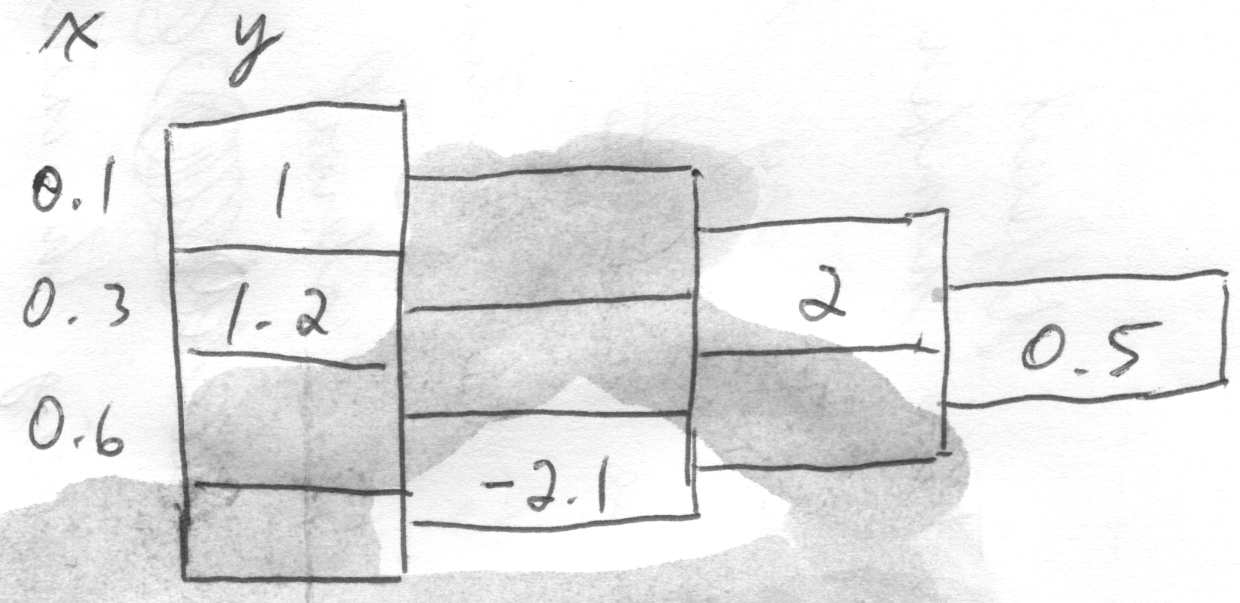
\includegraphics[width=6cm]{figures/interpolation-newton1}
\par\end{center}
\item Tunjukkan bahwa polinom yang menginterpolasi data berikut berderajat
3.

\begin{center}
\begin{tabular}{c|cccccc}
$x$ & $-2$ & $-1$ & $0$ & $1$ & $2$ & $3$\tabularnewline
\hline 
$f(x)$ & $1$ & $4$ & $11$ & $16$ & $13$ & $-4$\tabularnewline
\end{tabular}
\par\end{center}
\item \label{exc:interpolation-newton-11}Untuk fungsi $f$, rumus beda
terbagi Newton memberikan polinom interpolasi
\[
N_{3}(x)=1+4x+4x(x-0.25)+\frac{16}{3}x(x-0.25)(x-0.5)
\]
pada simpul $x_{0}=0$, $x_{1}=0.25$, $x_{2}=0.5$, $x_{3}=0.75$.
Carilah $f(0.75)$. \hasasolution 
\item \label{exc:interpolation-newton-12}Pasangkan fungsi dengan diagram
kekonvergenan metode Sidi dengan satu nilai awal. Dalam setiap kasus,
metode Sidi berderajat $6$ digunakan. Sumbu riil melewati pusat setiap
diagram, sedangkan sumbu imajiner ditampilkan, tetapi tidak selalu
berada di tengah. \hasasolution  
\begin{eqnarray*}
f(x) & = & \sin x\\
g(x) & = & \sin x-e^{-x}\\
h(x) & = & e^{x}+2^{-x}+2\cos x-6\\
l(x) & = & 56-152x+140x^{2}-17x^{3}-48x^{4}+9x^{5}
\end{eqnarray*}

\begin{center}
\begin{tabular}{cccc}
(a) &  & (b) & \tabularnewline
 & 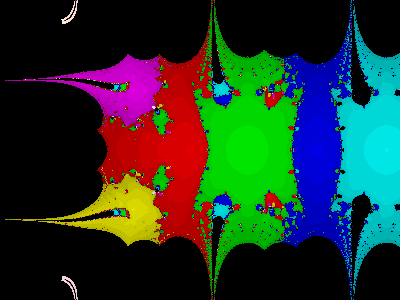
\includegraphics[scale=0.4]{figures/interpolation-newton2} &  & 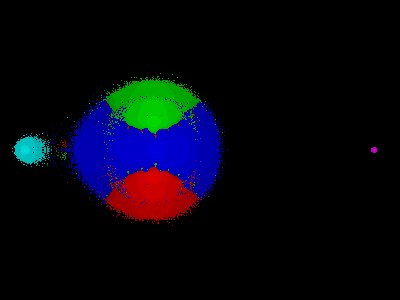
\includegraphics[scale=0.4]{figures/interpolation-newton5}\tabularnewline
(c) &  & (d) & \tabularnewline
 & 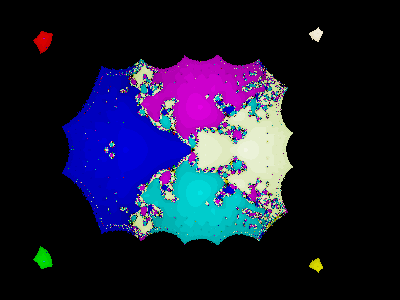
\includegraphics[scale=0.4]{figures/interpolation-newton4} &  & 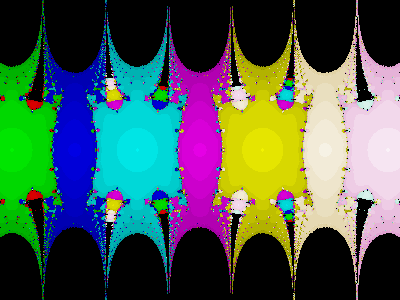
\includegraphics[scale=0.4]{figures/interpolation-newton3}\tabularnewline
\end{tabular}
\par\end{center}
\item \label{exc:interpolation-newton-13}Pasangkan fungsi dengan diagram
kekonvergenan metode Sidi dengan satu nilai awal. Sumbu riil melewati
pusat setiap diagram, sedangkan sumbu imajiner ditampilkan, tetapi
tidak selalu berada di tengah. \hasananswer 
\begin{eqnarray*}
f(x) & = & x^{4}+2x^{2}+4\\
g(x) & = & (x^{2})(\ln x)+(x-3)e^{x}\\
h(x) & = & 1+2x+3x^{2}+4x^{3}+5x^{4}+6x^{5}\\
l(x) & = & (\ln x)(x^{3}+1)
\end{eqnarray*}

\begin{center}
\begin{tabular}{cccc}
(a) &  & (b) & \tabularnewline
 & 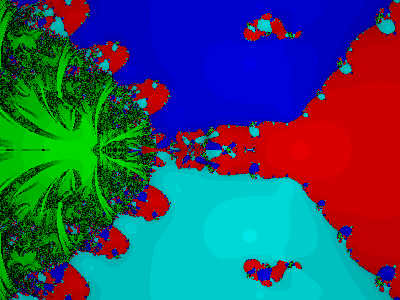
\includegraphics[scale=0.4]{figures/interpolation-newton8} &  & 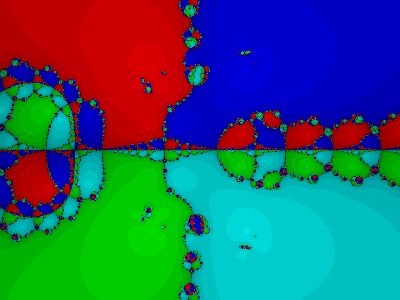
\includegraphics[scale=0.4]{figures/interpolation-newton9}\tabularnewline
(c) &  & (d) & \tabularnewline
 & 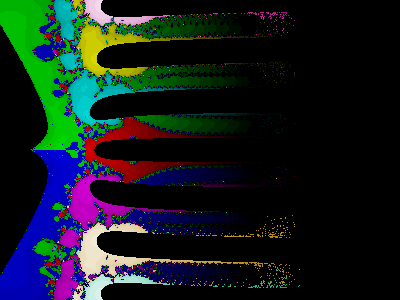
\includegraphics[scale=0.4]{figures/interpolation-newton6} &  & 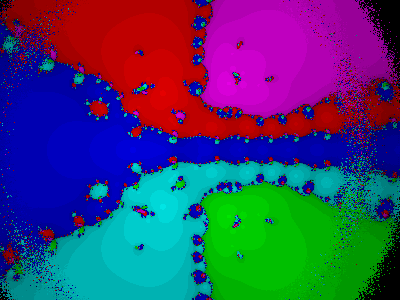
\includegraphics[scale=0.4]{figures/interpolation-newton7}\tabularnewline
\end{tabular}
\par\end{center}
\item Anda menemukan fungsi Octave berikut tanpa komentar (penulis fungsi
itu patut dicela!).

\begin{verbatim}
function ans = foo(x,y,x0)
  n = length(x);
  ans = 0;
  for i=1:n
    a=1;
    for j=1:n
      if (j==i)
        a=a*y(i);
      else
        a=a*(x0-x(j))/(x(i)-x(j));
      endif
    endfor
    ans=ans+a;
  endfor
endfunction
\end{verbatim}

Apa keluaran (\texttt{ans}) dari perintah Octave

\begin{center}
\texttt{foo({[}1.1,1.2,1.3,1.4{]},{[}.78,.81,.79,.75{]},1.2)} 
\par\end{center}

dan mengapa?
\end{enumerate}
\noindent\end{small}

\subsection{Jawaban}
\begin{description}
\item [{$P_{2}$~dari~$f_{1,0},f_{1,1},f_{0,2}$:}] \label{que:p2}$\overline{P}_{2}(x)=f_{1,0}+f_{1,1}(x-x_{1})+f_{0,2}(x-x_{1})(x-x_{2})$
\item [{$Q_{2}$~dua~cara~baru:}] \label{que:q2}$\hat{Q}_{2}(x)=f_{2,0}+f_{1,1}(x-x_{2})+f_{1,2}(x-x_{2})(x-x_{1})$
dan $\overline{Q}_{2}(x)=f_{2,0}+f_{2,1}(x-x_{2})+f_{1,2}(x-x_{2})(x-x_{3})$
\end{description}



% Chapter 4 -- Numerical Calculus 


\chapter{Kalkulus Numerik\label{chap:Numerical-Calculus}}

\section{\label{sec:NumericalRudiments}Dasar-Dasar Kalkulus Numerik}

\subsection{Gagasan dasar}

$g(x)=x-\frac{2\pi}{3}\sin(x)$ memiliki akar di antara $0$ dan $\pi$.
Anda sedang mencoba berbagai metode dan mulai tertarik pada bagaimana
pemilihan nilai awal memengaruhi hasilnya. Dengan menggunakan metode
Newton, Anda menyelidiki bagaimana pemilihan $x_{0}$ memengaruhi
$x_{2}$. Anda menjalankan beberapa pengujian dan memperoleh data
berikut.

\begin{center}
\begin{tabular}{c|c}
$x_{0}$ & $x_{2}$\tabularnewline
\hline 
$93/70$ & $2.084603181618954$\tabularnewline
$95/70$ & $2.055494116570853$\tabularnewline
$97/70$ & $2.030278824314539$\tabularnewline
$99/70$ & $2.009751835391139$\tabularnewline
$101/70$ & $1.993574976724822$\tabularnewline
$103/70$ & $1.981091507449763$\tabularnewline
$105/70$ & $1.971614474758557$\tabularnewline
\end{tabular}
\par\end{center}

\noindent Dengan menggunakan iterasi titik tetap pada $f(x)=\frac{2\pi}{3}\sin(x)$,
Anda memutuskan untuk menelaah bagaimana pemilihan $x_{0}$ memengaruhi
$x_{10}$, bukan $x_{2}$ karena iterasi titik tetap pada umumnya
lambat konvergen. Anda menjalankan beberapa pengujian atas metode
ini dan memperoleh data berikut.

\begin{center}
\begin{tabular}{c|c}
$x_{0}$ & $x_{10}$\tabularnewline
\hline 
$1/7$ & $1.949880891899200$\tabularnewline
$2/7$ & $1.951091775564697$\tabularnewline
$3/7$ & $1.923339403354019$\tabularnewline
$4/7$ & $1.941460911122824$\tabularnewline
$5/7$ & $1.960870620285721$\tabularnewline
$6/7$ & $1.965674866641883$\tabularnewline
$1$ & $1.961228252911260$\tabularnewline
\end{tabular}
\par\end{center}

Dalam eksperimen dengan metode Newton, $x_{2}$ merupakan fungsi dari
$x_{0}$, sedangkan dalam eksperimen iterasi titik tetap, $x_{10}$
merupakan fungsi dari $x_{0}$. Jadi, Anda mulai memandang keduanya
sepenuhnya terlepas dari persoalan pencarian akar semula. Dalam bentuk
tabelnya, keduanya hanyalah dua fungsi yang beberapa nilainya kita
ketahui, tetapi selebihnya tidak banyak. Seperti apakah bentuk fungsi-fungsi
ini? Apakah informasi yang kita miliki cukup untuk menemukan turunannya,
dan dengan demikian ekstrem lokalnya? Dapatkah kita menemukan antiturunannya?
Inilah pokok bahasan kalkulus numerik. Kita tentu dapat menghampiri
semua itu. 

Dalam bab \ref{chap:Interpolation} kita telah mempelajari cara menghampiri
fungsi dengan interpolasi, sehingga kita tahu bahwa data tabel dapat
digunakan untuk menghampiri fungsi itu sendiri. Namun, bagaimana dengan
turunan dan integralnya? Polinom mudah diturunkan dan diintegralkan.
Barangkali kita dapat menggunakan turunan dan integral polinom interpolasi
untuk menghampiri turunan dan integral $x_{2}(x_{0})$ dan $x_{10}(x_{0})$.
Ternyata memang bisa! 

Untuk menghindari kebingungan akibat penggunaan $x_{0}$ untuk beberapa
tujuan, fungsi-fungsi tersebut akan kita namai ulang sebagai $\nu(x)$
untuk $x_{2}(x_{0})$ dan $\varphi(x)$ untuk $x_{10}(x_{0})$. Dengan
demikian, kita memperoleh $\nu(93/70)=2.0846\ldots$, $\nu(95/70)=2.0554\ldots$,
dan seterusnya. Demikian pula, kini kita memperoleh $\varphi(1/7)=1.9498\ldots$,
$\varphi(2/7)=1.9510\ldots$, dan seterusnya. Kita juga akan membiasakan
diri menyebut koordinat-$x$ dari titik-titik interpolasi yang ditentukan
sebagai simpul.\index{simpul} Dengan demikian, simpul yang kita miliki
untuk $\nu$ adalah $93/70$, $95/70$, dan seterusnya. Simpul yang
kita miliki untuk $\varphi$ adalah $1/7$, $2/7$, dan seterusnya.

\noindent\begin{digression}{$\nu$ dan $\varphi$} 

\noindent$\nu$ adalah huruf ketiga belas (dalam bentuk huruf kecil)
dalam alfabet Yunani dan dilafalkan \texttt{nu}. $\varphi$ adalah
huruf kedua puluh satu (dalam bentuk huruf kecil) dalam alfabet Yunani
dan dilafalkan \texttt{fi}. Huruf \texttt{fi} juga ditulis sebagai
$\phi$, tetapi dalam matematika jauh lebih umum dijumpai bentuk varian
$\varphi$, mungkin untuk menghindari kerancuan antara \texttt{fi}
dan himpunan kosong, $\emptyset$. Bentuk huruf kapital dari $\nu$
dan $\varphi$ adalah $N$ dan $\Phi$, secara berturut-turut.

\noindent\end{digression}

Kita mulai dengan meninjau polinom interpolasi pada tiga simpul. Untuk
$\nu$, kita menggunakan simpul $93/70$, $99/70$, dan $1.5$, lalu
memperoleh
\[
P_{2,\nu}(x)=.07673215587088045x^{2}\text{\textminus}.07445530457646088x+1.95895140161684.
\]
Untuk $\varphi$, kita menggunakan simpul $1/7$, $4/7$, dan $1$,
lalu memperoleh
\[
P_{2,\varphi}(x)=2.498590686342254x^{2}-7.726543017101505x+7.939599956140455.
\]
Kita telah menambahkan subskrip kedua pada $P_{2}$ untuk membedakan
polinom interpolasi bagi $\nu$ dari polinom bagi $\varphi$. Kini
kita dapat menghampiri turunan dan integral dari $\nu$ dan $\varphi$
dengan menggunakan $P_{2,\nu}$ dan $P_{2,\varphi}$, secara berturut-turut:
\begin{eqnarray*}
\nu'(x) & \approx & P_{2,\nu}'(x)=4.997181372684508x-7.726543017101505\\
\varphi'(x) & \approx & P_{2,\varphi}'(x)=.1534643117417609x-.07445530457646088\\
\int\nu\,dx & \approx & \int P_{2,\nu}dx=.8328635621140847x^{3}-3.863271508550753x^{2}+7.939599956140455x+C\\
\int\varphi\,dx & \approx & \int P_{2,\varphi}dx=.02557738529029348x^{3}-.03722765228823044x^{2}+1.95895140161684x+D.
\end{eqnarray*}
Jadi, sebagai contoh,
\begin{eqnarray*}
\nu'(1.4) & \approx & P_{2,\nu}'(1.4)\\
 & = & 4.997181372684508(1.4)-7.726543017101505\\
 & = & -.7304890953431942\\
\varphi'(0.5) & \approx & P_{2,\varphi}'(0.5)\\
 & = & .1534643117417609(0.5)-.07445530457646088\\
 & = & .002276851294419568
\end{eqnarray*}
 dan 
\begin{eqnarray*}
\int_{1.4}^{1.5}\nu(x)dx & \approx & \int_{1.4}^{1.5}P_{2,\nu}(x)dx\\
 & = & \left[.8328635621140847x^{3}-3.863271508550753x^{2}+7.939599956140455x\right]_{1.4}^{1.5}\\
 & = & .1991481658283149\\
\int_{0}^{1}\varphi(x)dx & \approx & \int_{0}^{1}P_{2,\varphi}(x)dx\\
 & = & \left[.02557738529029348x^{3}-.03722765228823044x^{2}+1.95895140161684x\right]_{0}^{1}\\
 & = & 1.947301134618903.
\end{eqnarray*}

\noindent Selesai! Latihan ini merangkum seluruh strategi. Jika diberikan
beberapa nilai dari suatu fungsi yang selebihnya tidak diketahui,
kita akan menghampiri fungsi yang tidak diketahui itu dengan sebuah
polinom. Selanjutnya, kita akan menghampiri turunan dan integral fungsi
yang tidak diketahui dengan menurunkan dan mengintegralkan polinom
tersebut. Tidak banyak lagi yang perlu dikatakan tentang gagasan ini.
Namun, masih banyak yang perlu dibahas tentang otomasi, akurasi, dan
efisiensi, yang menjadi fokus sisa bab ini. Akan tetapi, sebelum menangani
persoalan tersebut, kita akan meninjau kembali $\nu$ dan $\varphi$.

Dengan menggunakan seluruh simpul $\nu$, dan dengan bantuan sistem
aljabar komputer, kita menghitung polinom interpolasi berderajat enam\label{integrationWithP6}
\begin{eqnarray*}
P_{6,\nu}(x) & = & -1342.393417879939x^{6}+11632.43754466623x^{5}-41996.4789301455x^{4}\\
 &  & +80851.91317212582x^{3}-87536.60487741232x^{2}+50528.3026241064x\\
 &  & -12144.27629915625.
\end{eqnarray*}
Dengan menggunakan seluruh simpul $\varphi$ (serta sistem aljabar
komputer), kita menghitung polinom interpolasi berderajat enam
\begin{eqnarray*}
P_{6,\varphi}(x) & = & -25.41848741926543x^{6}+97.00017832506126x^{5}-147.1805326076494x^{4}\\
 &  & +111.7996194440324x^{3}-43.71110414341027x^{2}+8.049781257197147x\\
 &  & +1.421773396945804.
\end{eqnarray*}
Sekali lagi, kita menambahkan subskrip kedua untuk membedakan polinom
interpolasi bagi $\nu$ dari polinom bagi $\varphi$. Kini kita dapat
memperoleh taksiran kedua untuk $\nu'(1.4)$, $\varphi'(0.6)$, $\int_{1.4}^{1.5}\nu\,dx$,
dan $\int_{0}^{1}\varphi\:dx$:
\begin{eqnarray*}
\nu'(1.4) & \approx & P_{6,\nu}'(1.4)\approx-.7178145479410887\\
\varphi'(0.5) & \approx & P_{6,\varphi}'(0.5)\approx.1729311759579151\\
\int_{1.4}^{1.5}\nu(x)dx & \approx & \int_{1.4}^{1.5}P_{6,\nu}(x)dx\approx.1991932206801721\\
\int_{0}^{1}\varphi(x)dx & \approx & \int_{0}^{1}P_{6,\varphi}(x)dx\approx1.925578216262883.
\end{eqnarray*}
Tabel \ref{tab:numericalCalcFirstStab} merangkum delapan taksiran
yang telah kita buat sejauh ini. 
\begin{table}
\hrule \caption{\label{tab:numericalCalcFirstStab}Penaksiran turunan dan integral
$\nu$ dan $\varphi$.}

\centering{}\medskip{}
\begin{tabular}{c|cc}
besaran & menggunakan $P_{2}$ & menggunakan $P_{6}$\tabularnewline
\hline 
$\nu'(1.4)$ & $-.7304890953431942$  & $-.7178145479410887$\tabularnewline
$\varphi'(0.5)$ & $.002276851294419568$  & $.1447147284558277$\tabularnewline
$\int_{1.4}^{1.5}\nu(x)dx$ & $.1991481658283149$ & $.1991932206801721$\tabularnewline
$\int_{0}^{1}\varphi(x)dx$ & $1.947301134618903$ & $1.925578216262883$\tabularnewline
\end{tabular}\medskip{}
\hrule 
\end{table}
Empat digit pertama pada taksiran $\int_{1.4}^{1.5}\nu(x)dx$ sama,
dan dua digit pertama pada taksiran $\int_{0}^{1}\varphi(x)dx$ sama.
Jadi, ada kesesuaian tertentu di antara taksiran integral tersebut.
Namun, taksiran turunannya tidak begitu selaras. Taksiran untuk $\nu'(1.4)$
hanya sama pada digit signifikan pertamanya. Keduanya menunjukkan
$\nu'(1.4)\approx-.7$. Namun, pada dasarnya tidak ada kesesuaian
antara taksiran $\varphi'(0.5)$. Salah satu hampiran bernilai lebih
dari 60 kali hampiran lainnya! Berdasarkan analisis sederhana ini,
kita akan sulit memercayai salah satu dari kedua taksiran $\varphi'(0.5)$.
Kita pun sebaiknya hanya memercayai beberapa digit pertama taksiran
lainnya. Kelak akan kita lihat bahwa perbandingan semacam ini dapat
digunakan agar komputer menentukan apakah suatu hampiran baik atau
tidak.

\subsection{Permasalahan}

Ada tiga permasalahan pada metode penaksiran turunan dan integral
yang baru saja diuraikan.
\begin{enumerate}
\item \textbf{Efisiensi.} Demi keperluan ilustrasi dan untuk memahami konsep
dasar kalkulus numerik, ada baiknya kita menghitung beberapa polinom
interpolasi seperti yang dilakukan pada subbagian sebelumnya. Namun,
cara tersebut rumit dan memakan waktu. Kita akan mencurahkan banyak
upaya untuk menemukan jalan pintas bagi metode langsung ini agar lebih
efisien dan praktis.
\item \textbf{Otomasi.} Metode numerik dimaksudkan untuk dijalankan oleh
komputer, bukan oleh manusia dengan kalkulator. Kita perlu menemukan
cara agar komputer dapat menangani polinom interpolasi. Permasalahan
ini berkaitan erat dengan efisiensi. Bagaimanapun, suatu algoritma
akan efisien jika dapat dieksekusi dengan cepat oleh komputer!
\item \textbf{Akurasi.} Sejauh ini, hampir tidak ada yang kita lakukan untuk
menentukan seberapa akurat hampiran kita. Kita perlu memahami suku
galat dengan lebih baik agar mengetahui cara menggunakan metode ini
secara akurat.
\end{enumerate}
Sekarang, kita mulai mengatasi ketiga permasalahan ini, tetapi sebagian
besar pembahasannya kita sisakan untuk bagian-bagian berikutnya.

Dalam bab \ref{chap:Interpolation}, kita memberi label pada simpul-simpul
suatu fungsi interpolasi sebagai $x_{0},x_{1},\ldots,x_{n}$. Akan
bermanfaat jika kita mulai menyebutnya $x_{0}+\theta_{0}h,x_{0}+\theta_{1}h,\ldots,x_{0}+\theta_{n}h$
sebagai gantinya. Untuk sebagian besar analisis, kita akan menggunakan
$x_{0}+\theta h$ alih-alih $x$ untuk titik tempat kita menginginkan
suatu taksiran. Substitusi ini dapat disebut perubahan variabel atau
kalibrasi ulang sumbu-$x$.

Untuk melihat bagaimana hal ini membantu analisis, tinjaulah polinom
interpolasi berderajat paling tinggi 2 untuk $f$ dengan simpul 
\[
x_{0}+\theta_{0}h,\ x_{0}+\theta_{1}h,\mbox{ dan }x_{0}+\theta_{2}h.
\]
Dalam notasi pada bab \ref{chap:Interpolation}, kita memperoleh 
\[
P_{2}(x)=\frac{(x-x_{1})(x-x_{2})}{(x_{0}-x_{1})(x_{0}-x_{2})}f(x_{0})+\frac{(x-x_{0})(x-x_{2})}{(x_{1}-x_{0})(x_{1}-x_{2})}f(x_{1})+\frac{(x-x_{0})(x-x_{1})}{(x_{2}-x_{0})(x_{2}-x_{1})}f(x_{2}),
\]
 tetapi dengan notasi baru, kita mengganti $x_{0}$ dengan $x_{0}+\theta_{0}h$,
$x_{1}$ dengan $x_{0}+\theta_{1}h$, $x_{2}$ dengan $x_{0}+\theta_{2}h$,
dan $x$ dengan $x_{0}+\theta h$, sehingga diperoleh
\begin{eqnarray}
P_{2}(x_{0}+\theta h) & = & \frac{(\theta-\theta_{1})(\theta-\theta_{2})}{(\theta_{0}-\theta_{1})(\theta_{0}-\theta_{2})}f(x_{0}+\theta_{0}h)\nonumber \\
 &  & +\frac{(\theta-\theta_{0})(\theta-\theta_{2})}{(\theta_{1}-\theta_{0})(\theta_{1}-\theta_{2})}f(x_{0}+\theta_{1}h)\nonumber \\
 &  & +\frac{(\theta-\theta_{0})(\theta-\theta_{1})}{(\theta_{2}-\theta_{0})(\theta_{2}-\theta_{1})}f(x_{0}+\theta_{2}h).\label{eq:p2relative}
\end{eqnarray}
Pada dasarnya, kita hanya menukar $x$ dengan $\theta$ dan $x_{i}$
dengan $\theta_{i}$. Perubahan yang tampak sepele ini sebenarnya
merupakan langkah maju yang sangat besar! Rumus ini memperlihatkan
bahwa nilai sebenarnya dari $x_{i}$ tidaklah penting. Yang penting
hanyalah letaknya relatif terhadap suatu titik acuan, $x_{0}$, yang
diukur dalam satuan panjang karakteristik $h$. $\theta$ dan $\theta_{i}$
merupakan ukuran tersebut. Pada hakikatnya, hal ini menjadikan $x_{0}$
sebagai titik asal dan $h$ sebagai satuan ukur pada sumbu-$x$. Kita
mengukur semua nilai dengan menghitung berapa kelipatan $h$ jaraknya
dari $x_{0}$.

Untuk menggambarkan manfaatnya, andaikan kita memiliki tiga simpul
yang berjarak sama, sehingga simpul terkecil dan terbesar berjarak
sama dari simpul ketiga, yaitu simpul tengah. Dengan menetapkan simpul
tengah sebagai titik acuan, $x_{0}$, dan panjang karakteristik, $h$,
sebagai jarak dari simpul tengah ini ke simpul lainnya, kita kemudian
dapat melabelinya sebagai
\[
x_{0}-h,\ x_{0},\mbox{ dan }x_{0}+h.
\]
Kita pun telah sampai pada hal pokok. Tidak menjadi masalah apakah
himpunan simpulnya adalah $\{1,2,3\}$ atau $\{80,90,100\}$ atau
$\{-4.3,-4.2,-4.1\}$. Dalam setiap himpunan tersebut, terdapat tiga
simpul, dan salah satunya merupakan titik tengah dari dua simpul lainnya.
Setiap himpunan simpul sama dengan himpunan $\{x_{0}-h,x_{0},x_{0}+h\}$
untuk nilai tertentu dari $x_{0}$ dan $h$. Dengan demikian, jika
kita dapat melakukan suatu analisis dengan himpunan $\{x_{0}-h,x_{0},x_{0}+h\}$,
kita memperoleh informasi tentang cara bekerja dengan himpunan simpul
mana pun, seperti $\{1,2,3\}$ atau $\{80,90,100\}$ atau $\{-4.3,-4.2,-4.1\}$
dan seterusnya. 

Kembali ke himpunan simpul $\{x_{0}-h,x_{0},x_{0}+h\}$. Untuk himpunan
simpul ini, kita memperoleh $\theta_{0}=-1$, $\theta_{1}=0$, dan
$\theta_{2}=1$. Dengan menyubstitusikannya ke \ref{eq:p2relative},
\begin{eqnarray*}
P_{2}(x_{0}+\theta h) & = & \frac{(\theta)(\theta-1)}{(-1)(-2)}f(x_{0}-h)+\frac{(\theta+1)(\theta-1)}{(1)(-1)}f(x_{0})+\frac{(\theta+1)(\theta)}{(2)(1)}f(x_{0}+h)\\
 & = & \frac{\theta^{2}-\theta}{2}f(x_{0}-h)+(1-\theta^{2})f(x_{0})+\frac{\theta^{2}+\theta}{2}f(x_{0}+h).
\end{eqnarray*}
Kini rumus ini dapat digunakan untuk memperoleh parabola interpolasi
pada sembarang himpunan tiga simpul yang berjarak sama. 

Untuk mencoba menerapkan rumus ini pada $\nu$, tinjaulah simpul $93/70$,
$99/70$, dan $105/70$. Karena $\frac{99}{70}-\frac{93}{70}=\frac{105}{70}-\frac{99}{70}$,
kita memiliki himpunan simpul berbentuk $\{x_{0}-h,x_{0},x_{0}+h\}$
dengan $x_{0}=\frac{99}{70}$ dan $h=\frac{6}{70}=\frac{3}{35}$.
Kebetulan $1.4=\frac{99}{70}-\frac{1}{6}\cdot\frac{3}{35}$, sehingga
kita menggunakan $\theta=-\frac{1}{6}$ untuk menghitung $P_{2,\nu}(1.4)$:
\begin{eqnarray*}
P_{2,\nu}(1.4) & = & P_{2,\nu}\left(x_{0}-\frac{1}{6}h\right)\\
 & = & \frac{\left(-\frac{1}{6}\right)^{2}+\frac{1}{6}}{2}\nu\left(\frac{93}{70}\right)+\left(1-\left(-\frac{1}{6}\right)^{2}\right)\nu\left(\frac{99}{70}\right)+\frac{\left(-\frac{1}{6}\right)^{2}-\frac{1}{6}}{2}\nu\left(\frac{105}{70}\right)\\
 & = & \frac{7\nu\left(\frac{93}{70}\right)+70\nu\left(\frac{99}{70}\right)-5\nu\left(\frac{105}{70}\right)}{72}\\
 & = & \frac{7(2.084603181618954)+70(2.009751835391139)-5(1.971614474758557)}{72}\\
 & = & 2.019677477429439.
\end{eqnarray*}
Taksiran ini tampak cukup baik karena nilainya berada di antara $\nu(93/70)\approx2.085$
dan $\nu(99/70)\approx2.009$ tetapi jauh lebih dekat ke $2.009$.
Bagaimanapun, $1.4$ berada di antara $93/70\approx1.328$ dan $99/70\approx1.414$
tetapi jauh lebih dekat ke $1.414$. Persamaan \ref{eq:lagrangeInterpolatingPolynomialError}
memberi kita gambaran tentang tingkat ketelitian yang dapat diharapkan
dari taksiran ini.

Namun, mari kita mundur beberapa langkah dalam perhitungan ini. Konstanta-konstanta
pada langkah $\frac{7\nu\left(\frac{93}{70}\right)+70\nu\left(\frac{99}{70}\right)-5\nu\left(\frac{105}{70}\right)}{72}$
ditentukan semata-mata dari nilai $\theta$ dan $\theta_{i}$. Sementara
itu, $\frac{93}{70}$, $\frac{99}{70}$, dan $\frac{105}{70}$ hanyalah
ketiga simpul, yaitu $x_{0}-h,x_{0},x_{0}+h$, sehingga yang sebenarnya
kita miliki di sini adalah suatu kaidah, atau rumus, untuk nilai $P_{2}(x_{0}-\frac{1}{6}h)$
bagi \textit{setiap} polinom interpolasi berderajat paling tinggi
2 pada simpul $x_{0}-h$, $x_{0}$, dan $x_{0}+h$:
\[
\nu\left(x_{0}-\frac{1}{6}h\right)\approx P_{2,\nu}\left(x_{0}-\frac{1}{6}h\right)=\frac{7\nu(x_{0}-h)+70\nu(x_{0})-5\nu(x_{0}+h)}{72}.
\]
Tidak ada pula yang istimewa pada fungsi $\nu$ yang digunakan dalam
rumus ini. Tidak satu pun dari konstanta $-\frac{1}{6}$, $7$, $70$,
$-5$, maupun $72$ bergantung pada $\nu$, melainkan hanya pada jarak
antarsimpul. Oleh karena itu, untuk sebarang fungsi $f$, dari perhitungan
ini kita dapat memperoleh rumus hampiran ringkas
\begin{equation}
f\left(x_{0}-\frac{1}{6}h\right)\approx\frac{7f(x_{0}-h)+70f(x_{0})-5f(x_{0}+h)}{72}.\label{eq:p2formula}
\end{equation}

\noindent Rumus ini menunjukkan tujuan sebenarnya dari menyatakan
ulang nilai $x_{i}$ dalam bentuk $x_{0}$, $h$, dan $\theta_{i}$.
Dengan cara ini, kita memperoleh rumus yang berlaku bagi seluruh kelas
simpul, bukan hanya satu himpunan simpul tertentu.

Untuk $\varphi$, simpul $\frac{1}{7}$, $\frac{4}{7}$, dan $1$
berjarak sama, sehingga himpunan $\{\frac{1}{7},\frac{4}{7},1\}$
memiliki bentuk $\{x_{0}-h,x_{0},x_{0}+h\}$ dengan $x_{0}=\frac{4}{7}$
dan $h=\frac{3}{7}$. Bukan suatu kebetulan bahwa $\frac{4}{7}-\frac{1}{6}\cdot\frac{3}{7}=0.5$,
sehingga $\varphi(0.5)=\varphi(x_{0}-\frac{1}{6}h)$ dengan $x_{0}=\frac{4}{7}$
dan $h=\frac{3}{7}$. Kini kita dapat menggunakan rumus \ref{eq:p2formula}
untuk menghampiri $\varphi(0.5)$!
\begin{eqnarray*}
\varphi(0.5) & \approx & P_{2,\varphi}(0.5)=\frac{7\varphi(x_{0}-h)+70\varphi(x_{0})-5\varphi(x_{0}+h)}{72}\\
 & = & \frac{7(1.9498808918992)+70(1.941460911122824)-5(1.96122825291126)}{72}\\
 & = & 1.94090678829633.
\end{eqnarray*}
Kali ini, kita sepenuhnya menghindari perhitungan dan evaluasi langsung
terhadap $P_{2,\varphi}$. Rumus \ref{eq:p2formula} memungkinkan
kita menghitung $P_{2,\varphi}(0.5)$ secara langsung dari nilai $\varphi$
pada ketiga simpul. Tidak perlu menghitung, merujuk kembali, mengevaluasi,
atau menyederhanakan $P_{2,\varphi}$! Semua itu telah dilakukan dalam
penurunan rumus. Sangat cepat. Sangat efisien.

\subsection{Stensil\index{stensil}}

Rumus seperti \ref{eq:p2formula} hanya berlaku untuk sekumpulan simpul
dan titik evaluasi yang memiliki geometri (posisi relatif) yang sama
dengan geometri yang digunakan untuk menurunkan rumus tersebut. Oleh
karena itu, kita perlu mencatat geometri yang digunakan untuk menurunkan
rumus-rumus semacam itu. Untuk keperluan tersebut, kita sering menyebut
sekumpulan simpul tertentu beserta titik evaluasinya sebagai stensil.
Sebagai contoh, simpul-simpul $x_{0}-h$, $x_{0}$, $x_{0}+h$ dengan
titik evaluasi $x_{0}-\frac{1}{6}h$ membentuk sebuah stensil---susunan
relatif titik-titik yang dapat diskalakan (dengan mengubah nilai $h$)
dan ditranslasikan (dengan mengubah nilai $x_{0}$). Pada garis bilangan,
stensil ini tampak seperti

\begin{center}
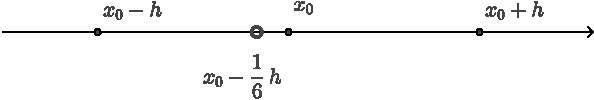
\includegraphics{figures/calculus-rudiments01}.
\par\end{center}

\noindent$x_{0}$ dapat berada di mana saja dan $h$ dapat bernilai
berapa pun, bahkan negatif. Fleksibilitas inilah yang membuat rumus
seperti \ref{eq:p2formula} berguna.

Sekarang, misalkan data yang kita miliki tidak berjarak sama, tetapi
kita tertarik pada sebuah titik di tengah-tengah dua titik lainnya.
Stensil tiga titik yang sesuai akan menggunakan simpul-simpul $x_{0}-h$,
yaitu simpul paling kiri, $x_{0}+h$, yaitu simpul paling kanan, dan
$x_{0}+\theta_{1}h$ untuk suatu $\theta_{1}$ di antara $-1$ dan
$1$, yaitu simpul tengah, dengan titik evaluasi $x_{0}$, yaitu titik
di tengah-tengah simpul paling kiri dan paling kanan. Untuk $\theta_{1}=\frac{1}{3}$,
stensil ini tampak seperti

\begin{center}
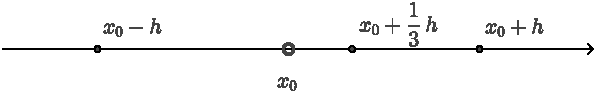
\includegraphics{figures/calculus-rudiments02}.
\par\end{center}

\noindent Kita juga dapat menurunkan rumus untuk $P_{2}(x_{0})$ berdasarkan
nilai $f$ pada ketiga simpul tersebut. Dengan menyubstitusikan $\theta=0$,
$\theta_{0}=-1$, $\theta_{1}=\frac{1}{3}$, dan $\theta_{2}=1$ ke
dalam persamaan \ref{eq:p2relative}, kita memperoleh
\begin{eqnarray*}
P_{2}(x_{0}) & = & \frac{(-\frac{1}{3})(-1)}{(-\frac{4}{3})(-2)}f(x_{0}-h)+\frac{(1)(-1)}{(\frac{4}{3})(-\frac{2}{3})}f(x_{0}+\frac{1}{3}h)+\frac{(1)(-\frac{1}{3})}{(2)(\frac{2}{3})}f(x_{0}+h)\\
 & = & \frac{f(x_{0}-h)+9f(x_{0}+\frac{1}{3}h)-2f(x_{0}+h)}{8},
\end{eqnarray*}
sekali lagi, sebuah rumus ringkas yang berlaku untuk fungsi $f$.
Tidak perlu menghitung polinom interpolasi atau mengevaluasinya secara
langsung untuk setiap data yang sesuai dengan stensil ini. Bagian
tersebut sudah dihitung dan disederhanakan.

\subsection{Turunan\label{subsec:Derivatives}\index{diferensiasi numerik}}

Rumus untuk turunan dapat diperoleh dengan cara yang sama. Setelah
diturunkan untuk suatu stensil, rumus tersebut dapat digunakan dengan
sangat mudah dan efisien untuk data lain yang sesuai dengan stensil
yang sama. Sekarang kita akan mencari rumus untuk turunan pertama,
$P_{2}'(x_{0}-\frac{1}{6}h)$, pada stensil

\begin{center}
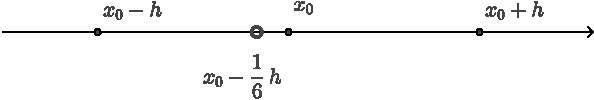
\includegraphics{figures/calculus-rudiments01}
\par\end{center}

\noindent yang digunakan sebelumnya. Kita mulai dengan mengamati bahwa
dalam \ref{eq:p2relative} $x$ merupakan fungsi dari $\theta$. Secara
khusus, $x(\theta)=x_{0}+h\theta$, sehingga $\frac{d}{d\theta}x(\theta)=h$.
Berdasarkan aturan rantai, $\frac{d}{d\theta}P_{2}(\theta)=\frac{d}{dx}P_{2}(x)\cdot\frac{d}{d\theta}x(\theta)=h\frac{d}{dx}P_{2}(x)$.
Dari persamaan \ref{eq:p2relative}, kita kemudian memperoleh 
\begin{eqnarray}
\frac{d}{dx}P_{2}(x) & = & \frac{\frac{d}{d\theta}P_{2}(\theta)}{h}\nonumber \\
 & = & \frac{(\theta-\theta_{1})+(\theta-\theta_{2})}{h(\theta_{0}-\theta_{1})(\theta_{0}-\theta_{2})}f(x_{0}+\theta_{0}h)\nonumber \\
 &  & +\frac{(\theta-\theta_{0})+(\theta-\theta_{2})}{h(\theta_{1}-\theta_{0})(\theta_{1}-\theta_{2})}f(x_{0}+\theta_{1}h)\nonumber \\
 &  & +\frac{(\theta-\theta_{0})+(\theta-\theta_{1})}{h(\theta_{2}-\theta_{0})(\theta_{2}-\theta_{1})}f(x_{0}+\theta_{2}h).\label{eq:p2relativeDerivative}
\end{eqnarray}
Secara khusus, ketika $\theta_{0}=-1$, $\theta_{1}=0$, $\theta_{2}=1$,
dan $\theta=-\frac{1}{6}$, kita memperoleh
\begin{eqnarray}
P_{2}'\left(x_{0}-\frac{1}{6}h\right) & = & \frac{-\frac{1}{6}-\frac{7}{6}}{h(-1)(-2)}f(x_{0}-h)+\frac{\frac{5}{6}-\frac{7}{6}}{h(1)(-1)}f(x_{0})+\frac{\frac{5}{6}-\frac{1}{6}}{h(2)(1)}f(x_{0}+h)\label{eq:derivativeDumb}\\
 & = & \frac{-2f(x_{0}-h)+f(x_{0})+f(x_{0}+h)}{3h}.\nonumber 
\end{eqnarray}
Kini kita memiliki rumus untuk $P_{2}'(x_{0}-\frac{1}{6}h)\approx f'(x_{0}-\frac{1}{6}h)$
pada stensil dengan simpul-simpul $x_{0}-h$, $x_{0}$, $x_{0}+h$
dan $x=x_{0}-\frac{1}{6}h$. Rumus ini sekarang dapat kita gunakan
untuk mengaproksimasi $\nu'(1.4)$ dan $\varphi'(0.5)$.
\begin{eqnarray*}
\nu'(1.4) & \approx & \frac{-2\nu(\frac{93}{70})+\nu(\frac{99}{70})+\nu(\frac{105}{70})}{3(\frac{3}{35})}\\
 & = & \frac{-2(2.084603181618954)+2.009751835391139+1.971614474758557)}{9/35}\\
 & = & -.7304890953430477.
\end{eqnarray*}
Perhatikan bahwa hasil ini tidak persis sama dengan yang kita peroleh
dalam tabel \ref{tab:numericalCalcFirstStab} untuk $\nu'(1.4)$ dengan
menggunakan $P_{2}$. Kedua taksiran tersebut berbeda pada beberapa
digit terakhir. Hal ini disebabkan oleh galat titik-mengambang yang
memengaruhi perhitungan dengan cara yang berbeda. Secara umum, perhitungan
langsung dari polinom interpolasi menghasilkan galat yang lebih besar
karena data diproses jauh lebih intensif. Namun, sebaiknya jangan
memercayai beberapa digit terakhir dalam kedua perhitungan. Selanjutnya,
\begin{eqnarray*}
\varphi'(0.5) & \approx & \frac{-2\varphi(\frac{1}{7})+\varphi(\frac{4}{7})+\varphi(1)}{3(\frac{3}{7})}\\
 & = & \frac{-2(1.9498808918992)+1.941460911122824+1.96122825291126)}{9/7}\\
 & = & .002276851294420679.
\end{eqnarray*}
Sekali lagi, hasil ini mendekati aproksimasi dalam tabel \ref{tab:numericalCalcFirstStab},
tetapi tidak persis sama karena galat titik-mengambang yang berbeda
dalam kedua perhitungan tersebut. Namun, inti pembahasannya sudah
jelas. Menggunakan rumus berbasis stensil lebih baik daripada bekerja
langsung dengan polinom interpolasi. Cara ini lebih mudah, lebih efisien,
dan dapat diotomatisasi.

Sebelum beralih ke integrasi, ada satu hal lagi yang perlu diperhatikan.
Ketika mencoba mengaproksimasi $f$ dengan polinom interpolasi, tidak
banyak gunanya mempertimbangkan stensil seperti

\begin{center}
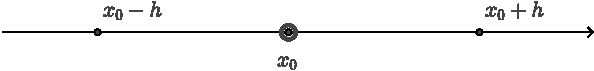
\includegraphics{figures/calculus-rudiments03},
\par\end{center}

\noindent yang titik evaluasinya merupakan salah satu simpul. Berdasarkan
definisi $P_{n}$, kita tahu bahwa $P_{n}(x_{i})=f(x_{i})$ untuk
setiap simpul $x_{i}$. Oleh karena itu, ``rumus'' tersebut adalah
$f(x_{i})=P_{2}(x_{i})$, dan rumus itu bersifat eksak, bukan aproksimasi.
Rumus ini juga tidak terlalu informatif karena fakta tersebut merupakan
salah satu dasar yang kita gunakan untuk menghitung $P_{2}$! Di sisi
lain, stensil semacam itu memang masuk akal ketika mencoba mengaproksimasi
turunan $f$. Tidak ada jaminan bahwa turunan $P_{n}$ akan sama dengan
turunan $f$ di titik mana pun, bahkan di simpul-simpulnya. Dengan
menyubstitusikan $\theta_{0}=-1$, $\theta_{1}=0$, $\theta_{2}=1$,
dan $\theta=0$ ke \ref{eq:p2relativeDerivative}, kita memperoleh
\begin{eqnarray}
P_{2}'(x_{0}) & = & \frac{1}{h(-1)(-2)}f(x_{0}-h)+\frac{1+(-1)}{h(1)(-1)}f(x_{0})+\frac{1}{h(2)(1)}f(x_{0}+h)\nonumber \\
 & = & \frac{f(x_{0}+h)-f(x_{0}-h)}{2h},\label{eq:centeredDifferenceNaive}
\end{eqnarray}
sebagai contoh.

\subsection{Integral\index{integrasi numerik}\index{integrasi numerik|seealso{kuadratur}}}

Untuk rumus integrasi, kita menggunakan stensil yang dimodifikasi.
Kita memerlukan simpul-simpul beserta ujung-ujung interval integrasi,
yang akan ditandai dengan tanda kurung siku: $[$ untuk ujung kiri
dan $]$ untuk ujung kanan. Namun, prosesnya serupa. Kita mencari
rumus untuk polinom interpolasi dan, alih-alih mengintegralkan fungsi
yang tidak diketahui, kita mengintegralkan polinom interpolasi.

Dengan mengikuti prosedur ini, kita dapat menurunkan rumus integral
untuk $f$ pada stensil 

\begin{center}
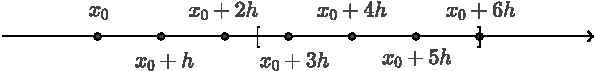
\includegraphics{figures/calculus-rudiments04},
\par\end{center}

\noindent sebagai contoh. Langkah-langkah aljabarnya sederhana tetapi
panjang, sehingga tidak kami tampilkan di sini. Sebaiknya gunakan
sistem aljabar komputer untuk menurunkan rumus semacam ini. Hasilnya,
yaitu aproksimasi integral pada $[x_{0}+2.5h,x_{0}+6h]$ dengan menggunakan
simpul-simpul $x_{0}$, $x_{0}+h$, $x_{0}+2h$, $x_{0}+3h$, $x_{0}+4h$,
$x_{0}+5h$, dan $x_{0}+6h$, adalah
\begin{eqnarray*}
\int_{x_{0}+2.5h}^{x_{0}+6h}f(x)dx & \approx & \frac{h}{138240}\left[42056f(x_{0}+6h)+201831f(x_{0}+5h)+63357f(x_{0}+4h)\right.\\
 &  & \left.+195902f(x_{0}+3h)-28518f(x_{0}+2h)+10731f(x_{0}+h)-1519f(x_{0})\right].
\end{eqnarray*}
Rumus ini kini dapat digunakan untuk mengaproksimasi $\int_{1.4}^{1.5}\nu(x)dx$
sebagai pengganti pengintegralan polinom interpolasi secara langsung
seperti yang dilakukan \vpageref{integrationWithP6}. Silakan substitusikan
nilai-nilai $\nu$ yang sesuai, lalu bandingkan jawaban Anda dengan
jawaban pada tabel \vpageref{tab:numericalCalcFirstStab}. Jawaban
\vpageref{ans:integralFormula1}.

Stensil untuk aproksimasi $\int_{0}^{1}\varphi(x)dx$ menggunakan
$P_{6,\varphi}$ tampak seperti 

\begin{center}
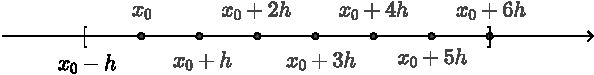
\includegraphics{figures/calculus-rudiments05},
\par\end{center}

\noindent yang berbeda dari stensil yang kita gunakan untuk mengaproksimasi
$\int_{1.4}^{1.5}\nu(x)dx$. Oleh karena itu, rumus aproksimasinya
juga berbeda. Kita memerlukan rumus integral pada $[x_{0}-h,x_{0}+6h]$
dengan simpul-simpul $x_{0}$, $x_{0}+h$, $x_{0}+2h$, $x_{0}+3h$,
$x_{0}+4h$, $x_{0}+5h$, dan $x_{0}+6h$. Simpul-simpulnya sama seperti
sebelumnya, tetapi interval integrasinya berbeda. Hasilnya adalah
\begin{eqnarray}
\int_{x_{0}-h}^{x_{0}+6h}f(x)dx & \approx & \frac{h}{8640}\left[5257f(x_{0}+6h)-5880f(x_{0}+5h)+59829f(x_{0}+4h)\right.\nonumber \\
 &  & \left.-81536f(x_{0}+3h)+102459f(x_{0}+2h)-50568f(x_{0}+h)+30919f(x_{0})\right].\label{eq:integral7dumb}
\end{eqnarray}
Sekali lagi, rumus semacam ini sebaiknya diturunkan dengan menggunakan
sistem aljabar komputer. Silakan substitusikan nilai-nilai $\varphi$
yang sesuai untuk mengaproksimasi $\int_{0}^{1}\varphi(x)dx$ dan
bandingkan hasil Anda dengan hasil pada tabel \vpageref{tab:numericalCalcFirstStab}.
Jawaban \vpageref{ans:integralFormula2}.

\subsection{Konsep Kunci}
\begin{description}
\item [{simpul:}] \index{simpul}absis (koordinat pertama) suatu titik
data yang digunakan dalam interpolasi.
\item [{aproksimasi~polinomial:}] \index{aproksimasi polinomial}mengaproksimasi
nilai suatu fungsi, turunannya, atau integralnya berdasarkan nilai
yang bersesuaian dari suatu polinom interpolasi.
\item [{stensil:}] \index{stensil}susunan relatif absis yang digunakan
dalam aproksimasi polinomial.
\end{description}
\noindent\startexercises 

\subsection{Latihan}
\begin{enumerate}
\item Buatlah sketsa stensil yang sesuai dengan rumus tersebut (dan yang
mungkin menjadi dasar penurunan rumus itu).
\begin{enumerate}
\item $f''\left(x_{0}+\frac{1}{2}h\right)\approx\frac{f(x_{0}+2h)-2f(x_{0}+h)+f(x_{0})}{h^{2}}$
\item $f'(x_{0})\approx\frac{-5f(x_{0}-h)+8f(x_{0}+2h)-3f(x_{0}+3h)}{12h}$
\item \label{exc:rudiments-29}$\int_{x_{0}}^{x_{0}+2h}f(x)dx\approx\frac{2h}{3}\left[f\left(x_{0}+\frac{1}{3}h\right)+2f\left(x_{0}+\frac{4}{3}h\right)\right]$ \hasasolution 
\item $f'\left(x_{0}-h\right)\approx\frac{-3f(x_{0}-h)+4f(x_{0})-f(x_{0}+h)}{2h}$
\item \label{exc:rudiments-30}$f''\left(x_{0}+\frac{1}{2}h\right)\approx\frac{2f(x_{0})-8f(x_{0}+h)+8f(x_{0}+\frac{3}{2}h)-2f(x_{0}+2h)}{h^{2}}$ \hasasolution 
\item $\int_{x_{0}}^{x_{0}+2h}f(x)dx\approx\frac{h}{2}\left(3f\left(x_{0}+\frac{2}{3}h\right)+f(x_{0}+2h)\right)$
\end{enumerate}
\item Gambarkan suatu stensil sehingga data berikut (beserta rumus yang
diturunkan untuk stensil tersebut) dapat digunakan untuk menghampiri
$f'(1)$.
\begin{enumerate}
\item %
\begin{tabular}{c|cccc}
$x$ & $0.5$ & $1.0$ & $1.5$ & $2.0$\tabularnewline
\hline 
$f(x)$ & $0.095$ & $0.191$ & $0.552$ & $1.110$\tabularnewline
\end{tabular}
\item \label{exc:rudiments-31}%
\begin{tabular}{c|cccc}
$x$ & $0$ & $1$ & $2$ & $3$\tabularnewline
\hline 
$f(x)$ & $3.05$ & $3.12$ & $3.45$ & $4.26$\tabularnewline
\end{tabular} \hasasolution 
\item %
\begin{tabular}{c|ccc}
$x$ & $0$ & $2$ & $3$\tabularnewline
\hline 
$f(x)$ & $4.92$ & $4.44$ & $4.37$\tabularnewline
\end{tabular}
\item \label{exc:rudiments-32}%
\begin{tabular}{c|ccc}
$x$ & $0$ & $1.5$ & $3$\tabularnewline
\hline 
$f(x)$ & $4.92$ & $4.44$ & $4.37$\tabularnewline
\end{tabular} \hasasolution 
\item %
\begin{tabular}{c|cccc}
$x$ & $0.3$ & $0.6$ & $0.9$ & $1.2$\tabularnewline
\hline 
$f(x)$ & $2.02$ & $2.10$ & $2.16$ & $2.23$\tabularnewline
\end{tabular}
\end{enumerate}
\item Gambarkan suatu stensil sehingga data berikut (beserta rumus yang
diturunkan untuk stensil tersebut) dapat digunakan untuk menghampiri
$\int_{1}^{5}f(x)dx$.
\begin{enumerate}
\item %
\begin{tabular}{c|cccc}
$x$ & $1$ & $2$ & $3$ & $4$\tabularnewline
\hline 
$f(x)$ & $0.095$ & $0.191$ & $0.552$ & $1.110$\tabularnewline
\end{tabular}
\item \label{exc:rudiments-33}%
\begin{tabular}{c|cccc}
$x$ & $1.5$ & $2.5$ & $3.5$ & $4.5$\tabularnewline
\hline 
$f(x)$ & $3.05$ & $3.12$ & $3.45$ & $4.26$\tabularnewline
\end{tabular} \hasasolution 
\item %
\begin{tabular}{c|ccc}
$x$ & $1$ & $2$ & $4$\tabularnewline
\hline 
$f(x)$ & $4.92$ & $4.44$ & $4.37$\tabularnewline
\end{tabular}
\item \label{exc:rudiments-34}%
\begin{tabular}{c|ccc}
$x$ & $1.2$ & $2.4$ & $3.6$\tabularnewline
\hline 
$f(x)$ & $4.92$ & $4.44$ & $4.37$\tabularnewline
\end{tabular} \hasasolution 
\item %
\begin{tabular}{c|cccc}
$x$ & $1.3$ & $2.6$ & $3.9$ & $4.2$\tabularnewline
\hline 
$f(x)$ & $2.02$ & $2.10$ & $2.16$ & $2.23$\tabularnewline
\end{tabular}
\end{enumerate}
\item \label{exc:rudiments}Turunkan rumus hampiran untuk turunan pertama
pada stensil

\begin{center}
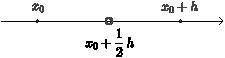
\includegraphics{figures/calculus-rudiments06}
\par\end{center}

dengan mengikuti langkah-langkah berikut. \hasasolution 
\begin{enumerate}
\item Tuliskan $L_{1}(x)$, yaitu bentuk Lagrange dari polinom interpolasi
yang melalui titik-titik
\[
(x_{0},f(x_{0}))\quad\mbox{dan}\quad(x_{1},f(x_{1})).
\]
\item Hitung turunan $L_{1}'(x)$.
\item Substitusikan $x_{0}+\frac{1}{2}h$ untuk $x$ dan $x_{0}+h$ untuk
$x_{1}$ ke dalam rumus yang Anda peroleh pada bagian (b), lalu sederhanakan.
\end{enumerate}
\item Turunkan rumus hampiran untuk turunan pertama pada stensil

\begin{center}
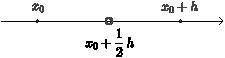
\includegraphics{figures/calculus-rudiments06}
\par\end{center}

dengan mengikuti langkah-langkah berikut.
\begin{enumerate}
\item Tuliskan $L_{1}(x(\theta))=L_{1}(x_{0}+\theta h)$, yaitu bentuk Lagrange
dari polinom interpolasi yang melalui titik-titik
\[
(x_{0},f(x_{0}))\quad\mbox{dan}\quad(x_{0}+h,f(x_{0}+h))
\]
dalam bentuk $\theta$, $h$, dan $x_{0}$.
\item Hitung turunan $\frac{d}{dx}L_{1}(x(\theta))$. Ingat bahwa $x(\theta)=x_{0}+\theta h$,
lalu gunakan aturan rantai.
\item \label{exc:rudiments-4}Substitusikan $\theta=\frac{1}{2}$ ke dalam
rumus yang Anda peroleh pada bagian (b), lalu sederhanakan. \hasananswer 
\end{enumerate}
\item Turunkan rumus hampiran untuk turunan pertama pada stensil

\begin{center}
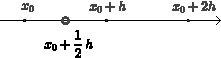
\includegraphics{figures/calculus-rudiments21}
\par\end{center}

 dengan mengikuti langkah-langkah berikut.
\begin{enumerate}
\item Hitung $N_{2}(x)$, yaitu bentuk Newton dari polinom interpolasi yang
melalui titik-titik
\[
(x_{0},f(x_{0})),\ (x_{1},f(x_{1})),\ \mbox{dan}\ (x_{2},f(x_{2})).
\]
\item Hitung turunan $N_{2}'(x)$.
\item \label{exc:rudiments-5}Substitusikan $x_{0}+\frac{1}{2}h$ untuk
$x$, $x_{0}+h$ untuk $x_{1}$, dan $x_{0}+2h$ untuk $x_{2}$ ke
dalam rumus yang Anda peroleh pada bagian (b), lalu sederhanakan. \hasananswer 
\end{enumerate}
\item \label{exc:rudiments-6}Turunkan rumus hampiran untuk turunan kedua
pada stensil

\begin{center}
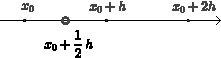
\includegraphics{figures/calculus-rudiments21}
\par\end{center}

dengan mengikuti langkah-langkah berikut. \hasasolution 
\begin{enumerate}
\item Hitung $N_{2}(x(\theta))=N_{2}(x_{0}+\theta h)$, yaitu bentuk Newton
dari polinom interpolasi yang melalui titik-titik
\[
\begin{gathered}(x_{0},f(x_{0})),\ (x_{0}+h,f(x_{0}+h)),\\
\mbox{dan}\ (x_{0}+2h,f(x_{0}+2h))
\end{gathered}
\]
dalam bentuk $\theta$, $h$, dan $x_{0}$.
\item Hitung turunan $\frac{d^{2}}{dx^{2}}N_{2}(x(\theta))$. Ingat bahwa
$x(\theta)=x_{0}+\theta h$, lalu gunakan aturan rantai.
\item Substitusikan $\theta=\frac{1}{2}$ ke dalam rumus yang Anda peroleh
pada bagian (b), lalu sederhanakan.
\end{enumerate}
\item Rumus \ref{eq:centeredDifferenceNaive} dan rumus yang Anda peroleh
dari soal \ref{exc:rudiments} seharusnya berbeda. Namun, keduanya
diturunkan pada stensil yang pada dasarnya sama---dua simpul dengan
titik evaluasi yang berada tepat di tengah keduanya. Hanya label pada
stensil tersebut yang berbeda. Dengan kata lain, keduanya diturunkan
dari geometri yang sama sehingga, dalam arti tertentu, keduanya pasti
sama. Dalam soal \ref{exc:rudiments}, $x_{0}$ memiliki peran yang
sama dengan $x_{0}-h$ dalam \ref{eq:centeredDifferenceNaive}. Selain
itu, dalam soal \ref{exc:rudiments}, jarak dari titik evaluasi ke
masing-masing simpul adalah $\frac{h}{2}$ sedangkan dalam \ref{eq:centeredDifferenceNaive},
jarak tersebut adalah $h$. Lakukan substitusi $x_{0}$ untuk $x_{0}-h$
dalam \ref{eq:centeredDifferenceNaive}. Kemudian substitusikan $\frac{h}{2}$
untuk $h$ pada penyebut \ref{eq:centeredDifferenceNaive}. Dengan
substitusi ini, rumus \ref{eq:centeredDifferenceNaive} seharusnya
sama persis dengan rumus yang Anda peroleh dalam soal \ref{exc:rudiments}.
Dengan kata lain, pelabelan yang berbeda pada suatu stensil menghasilkan
pelabelan yang berbeda pada rumus terkait. Tidak lebih dari itu.
\item \label{exc:rudiments-1}Gunakan rumus \ref{eq:integral7dumb} untuk
menghampiri integral berikut.

\begin{enumerate}
\item \label{exc:rudiments-7}${\displaystyle \int_{-4}^{3}e^{x}dx}$ \hasananswer 
\item ${\displaystyle \int_{-1}^{6}\sin x\,dx}$
\item \label{exc:rudiments-8}${\displaystyle \int_{10}^{17}\frac{1}{x-5}dx}$
 \hasasolution 
\item ${\displaystyle \int_{-3}^{4}\left(x^{5}-4\right)dx}$
\item \label{exc:rudiments-9}${\displaystyle \int_{0}^{1}e^{-x}dx}$ \hasananswer 
\item ${\displaystyle \int_{-\pi/2}^{\pi/2}\cos x\,dx}$
\item \label{exc:rudiments-10}${\displaystyle \int_{1}^{2}\frac{1}{x}dx}$ \hasananswer 
\item ${\displaystyle \int_{4}^{6.1}\left(9-x^{4}\right)dx}$
\end{enumerate}
\item \label{exc:rudiments-11}Untuk setiap integral pada soal \ref{exc:rudiments-1},
(i) hitung integral tersebut secara eksak, dan (ii) hitung galat absolut
pada hampirannya. \haspartwithsolution  \haspartwithanswer 
\item \label{exc:rudiments-2}Misalkan $f(x)=(x-1)^{2}\sin x$. Gunakan
rumus \ref{eq:derivativeDumb} untuk menghampiri $f'(0)$ dengan menggunakan

\begin{enumerate}
\item $h=1$
\item \label{exc:rudiments-12}$h=\frac{1}{2}$ \hasananswer 
\item $h=\frac{1}{4}$
\item $h=\frac{1}{8}$
\end{enumerate}
\item \label{exc:rudiments-13}Hitung galat absolut pada setiap hampiran
dalam soal \ref{exc:rudiments-2}. Apakah galat tersebut mengecil
ketika $h$ mengecil? \haspartwithanswer 
\item \label{exc:rudiments-28}Turunkan rumus hampiran pada stensil

\begin{center}
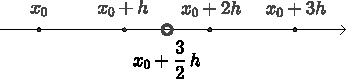
\includegraphics{figures/calculus-rudiments07}
\par\end{center}
\begin{enumerate}
\item untuk nilai fungsi.
\item untuk turunan pertama.
\item untuk turunan kedua.
\item untuk turunan ketiga. Apa yang dapat Anda simpulkan tentang rumus
ini?
\end{enumerate}
\item Polinom $p(x)=3x^{4}-2x^{2}+x-7$ adalah polinom interpolasi untuk
$f$. Gunakan $p$ untuk mengaproksimasi

\begin{enumerate}
\item $f(1)$
\item \label{exc:rudiments-14}$f(2)$ \hasananswer 
\item $f'(1)$
\item \label{exc:rudiments-15}$f'(2)$ \hasasolution 
\item ${\displaystyle \int_{0}^{1}f(x)dx}$
\item \label{exc:rudiments-16}${\displaystyle \int_{0}^{2}f(x)dx}$ \hasananswer 
\end{enumerate}
\item Polinom $q(x)=-7x^{4}+3x^{2}-x+4$ adalah polinom interpolasi untuk
$g$. Gunakan $q$ untuk mengaproksimasi

\begin{enumerate}
\item \label{exc:rudiments-17}$g(1)$ \hasananswer 
\item $g(2)$
\item \label{exc:rudiments-18}$g'(1)$ \hasananswer 
\item $g'(2)$
\item \label{exc:rudiments-19}${\displaystyle \int_{0}^{1}g(x)dx}$ \hasasolution 
\item ${\displaystyle \int_{0}^{2}g(x)dx}$
\end{enumerate}
\item Gunakan \ref{eq:p2relativeDerivative} untuk menentukan rumus turunan
pertama pada stensil

\begin{enumerate}
\item \raisepic{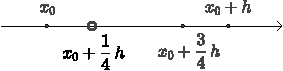
\includegraphics{figures/calculus-rudiments08}}\medskip 
\item \label{exc:rudiments-20}\raisepic{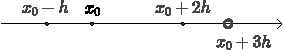
\includegraphics{figures/calculus-rudiments10}}\medskip  \hasananswer 
\item \raisepic{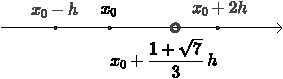
\includegraphics{figures/calculus-rudiments11}}\medskip 
\item \label{exc:rudiments-21}\raisepic{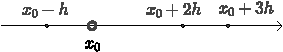
\includegraphics{figures/calculus-rudiments09}}\medskip  \hasasolution 
\item \raisepic{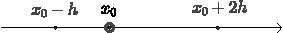
\includegraphics{figures/calculus-rudiments12}}\medskip 
\item \label{exc:rudiments-22}\raisepic{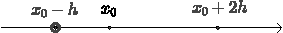
\includegraphics{figures/calculus-rudiments15}}\medskip  \hasananswer 
\item \raisepic{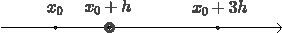
\includegraphics{figures/calculus-rudiments13}}\medskip 
\item \label{exc:rudiments-23}\raisepic{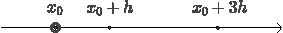
\includegraphics{figures/calculus-rudiments14}} \hasananswer 
\end{enumerate}
\item \label{exc:rudiments-3}Tentukan rumus hampiran umum untuk integral
dengan menggunakan dua simpul melalui langkah-langkah berikut.

\begin{enumerate}
\item Tuliskan polinom interpolasi linear dengan simpul-simpul $x_{0}+\theta_{2}h$
dan $x_{0}+\theta_{3}h$.
\item Integralkan polinom tersebut pada interval $[x_{0}+\theta_{0}h,x_{0}+\theta_{1}h]$.
\item \label{exc:rudiments-24}Sederhanakan. \hasananswer 
\end{enumerate}
\item Gunakan rumus hampiran umum yang Anda turunkan dalam soal \ref{exc:rudiments-3}
untuk memperoleh rumus hampiran pada stensil.

\begin{enumerate}
\item \label{exc:rudiments-25}\raisepic{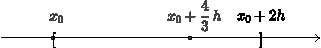
\includegraphics{figures/calculus-rudiments16}}\medskip  \hasananswer 
\item \raisepic{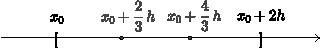
\includegraphics{figures/calculus-rudiments17}}\medskip 
\item \label{exc:rudiments-26}\raisepic{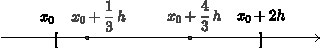
\includegraphics{figures/calculus-rudiments18}}\medskip  \hasasolution 
\item \raisepic{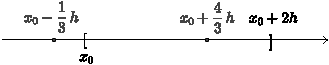
\includegraphics{figures/calculus-rudiments19}}\medskip 
\item \label{exc:rudiments-27}\raisepic{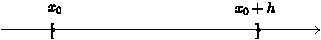
\includegraphics{figures/calculus-rudiments20}} \hasananswer 
\end{enumerate}
\item Rumus umum tiga titik untuk turunan pertama yang menggunakan $f(x_{0})$,
$f(x_{0}+\alpha h)$, dan $f(x_{0}+2h)$, dengan $\alpha\neq0$ dan
$\alpha\neq2$, diberikan oleh
\begin{eqnarray*}
f'(x_{0}) & = & \frac{1}{2h}\left[-\frac{2+\alpha}{\alpha}f(x_{0})\right.\\
 &  & \qquad+\frac{4}{\alpha(2-\alpha)}f(x_{0}+\alpha h)\\
 &  & \qquad\left.-\frac{\alpha}{2-\alpha}f(x_{0}+2h)\right]+O(h^{2})
\end{eqnarray*}

Gunakan ekspansi Taylor dari $f(x_{0}+\alpha h)$ dan $f(x_{0}+2h)$
untuk menurunkan rumus yang diberikan.
\end{enumerate}
\noindent\finishexercises 

\subsection{Jawaban}
\begin{description}
\item [{\textmd{$\int_{x_{0}+2.5h}^{x_{0}+6h}f(x)dx$:\label{ans:integralFormula1}}}] 
\[
\begin{gathered}\frac{1/35}{138240}\left[42056(1.971614474758557)+201831(1.981091507449763)\right.\\
+63357(1.993574976724822)+195902(2.009751835391139)\\
-28518(2.030278824314539)+10731(2.055494116570853)\\
\left.-1519(2.084603181618954)\right]
\end{gathered}
\]
 
\item [{$\int_{x_{0}-h}^{x_{0}+6h}f(x)dx$:\label{ans:integralFormula2}}] 
\[
\begin{gathered}\frac{1/7}{8640}\left[5257(1.96122825291126)-5880(1.965674866641883)\right.\\
+59829(1.960870620285721)-81536(1.941460911122824)\\
+102459(1.923339403354019)-50568(1.951091775564697)\\
\left.+30919(1.9498808918992)\right]
\end{gathered}
\]
\end{description}


\section{\label{sec:UndeterminedCoefficients}Koefisien Tak Tentu\index{koefisien tak tentu}}

\subsection{Gagasan dasar}

Menurut persamaan \ref{eq:lagrangeInterpolatingPolynomialError},
selisih antara $f$ dan suatu polinom interpolasi merupakan kelipatan
dari $f^{(n+1)}(\xi_{x})$. Dengan kata lain, galat dalam mengaproksimasi
$f$ dengan polinom interpolasi $P_{n}$ bergantung langsung pada
$f^{(n+1)}$. Namun, $f^{(n+1)}(x)$ identik nol setiap kali $f$
merupakan polinom berderajat kurang dari $n+1$. Akibatnya, $(f-P_{n})(x)$
identik nol dalam kasus ini. Meskipun terdengar berulang, gagasan
terakhir ini layak ditegaskan kembali. Jika $f$ adalah sembarang
polinom berderajat kurang dari $n+1$, maka $P_{n}$, yang dihitung
untuk sembarang himpunan yang terdiri dari $n+1$ simpul, sama persis
dengan $f$ untuk semua $x$. Dengan demikian, turunan $P_{n}$ dan
integral $P_{n}$ bukan sekadar aproksimasi terhadap turunan dan integral
yang bersesuaian dari $f$. Keduanya eksak karena $P_{n}=f$ untuk
semua $x$. Pengamatan ini dapat digunakan untuk menurunkan rumus
turunan dan integral tanpa pernah menghitung $P_{n}$ maupun turunan
atau integralnya!

Semua rumus yang telah kita turunkan untuk mengaproksimasi turunan
dan integral dari fungsi sembarang $f$ berbentuk
\[
\sum_{i=0}^{n}a_{i}f(x_{i})
\]
dengan $x_{0},x_{1},\ldots,x_{n}$ adalah simpul-simpul polinom interpolasi,
yaitu titik-titik tempat nilai $f$ diketahui, sedangkan $a_{i}$
adalah konstanta yang diperoleh dari penurunan tersebut. Metode koefisien
tak tentu menggunakan pendekatan langsung untuk menghitung konstanta
$a_{i}$. Dengan mengetahui bahwa rumus ``aproksimasi'' harus eksak
untuk semua polinom berderajat $0,1,\ldots,n$, kita dapat membentuk
$n+1$ persamaan dengan $n+1$ peubah tak diketahui, yaitu $a_{0},a_{1},\ldots,a_{n}$.
Penyelesaian sistem persamaan yang dihasilkan memberikan nilai koefisien
tersebut.

\subsection{Turunan\index{diferensiasi numerik}}

Kita mencari aproksimasi untuk turunan orde $k$ dari $f$ berdasarkan
nilai-nilai yang diketahui, yaitu $f(x_{0}+\theta_{0}h),f(x_{0}+\theta_{1}h),\ldots,f(x_{0}+\theta_{n}h)$.
Secara tepat, kita menginginkan aproksimasi berbentuk
\begin{equation}
f^{(k)}(x_{0}+\theta h)\approx\sum_{i=0}^{n}a_{i}f(x_{0}+\theta_{i}h).\label{eq:derivApprox}
\end{equation}
Berdasarkan persamaan \ref{eq:lagrangeInterpolatingPolynomialError},
aproksimasi tersebut harus eksak untuk semua polinom berderajat $n$
atau kurang. Secara khusus, aproksimasi itu harus eksak untuk polinom
$p_{j}(x)=(x-x_{0})^{j}$, $j=0,1,\ldots,n$. Secara simbolis, harus
berlaku
\[
p_{j}^{(k)}(x_{0}+\theta h)=\sum_{i=0}^{n}a_{i}p_{j}(x_{0}+\theta_{i}h)
\]
untuk $j=0,1,\ldots,n$. Perhatikan bahwa aproksimasi tersebut kini
menjadi suatu kesamaan \textit{eksak}. Dengan memperhatikan bahwa
$p_{j}(x_{0}+\theta_{i}h)=((x_{0}+\theta_{i}h)-x_{0})^{j}=(\theta_{i}h)^{j}$,
sistem persamaan tersebut menjadi
\begin{equation}
p_{j}^{(k)}(x_{0}+\theta h)=a_{0}+\sum_{i=1}^{n}(\theta_{i}h)^{j}a_{i}\label{eq:systemGenericDerivative}
\end{equation}
untuk $j=0,1,\ldots,n$. Penyelesaian sistem inilah yang akan menghasilkan
$a_{i}$.

\noindent\begin{digression}{Matriks Vandermonde}

\noindent Secara umum, suatu sistem persamaan linear mungkin memiliki
nol, satu, atau banyak penyelesaian. Namun, sistem \ref{eq:systemGenericDerivative}
memiliki bentuk khusus. Dalam setiap persamaan, konstanta $(\theta_{i}h)^{j}$
membentuk barisan geometri. Matriks koefisien seperti ini disebut
matriks Vandermonde, dan diketahui bahwa selama $\theta_{i}$ saling
berbeda, sistem ini akan memiliki satu penyelesaian. 

\noindent\end{digression}

Sebagai ilustrasi, misalkan kita memiliki stensil 

\begin{center}
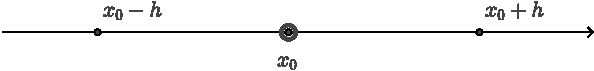
\includegraphics{figures/calculus-rudiments03}
\par\end{center}

\noindent dan kita ingin memperoleh rumus untuk turunan pertama dan
kedua dari $f$ (pada $x_{0}$). Untuk stensil ini, $\theta=0$, $\theta_{0}=-1$,
$\theta_{1}=0$, serta $\theta_{2}=1$, sehingga kita mencari rumus
dengan bentuk
\begin{eqnarray*}
f'(x_{0}) & \approx & a_{0}f(x_{0}-h)+a_{1}f(x_{0})+a_{2}f(x_{0}+h)\\
 &  & \mbox{ dan}\\
f''(x_{0}) & \approx & b_{0}f(x_{0}-h)+b_{1}f(x_{0})+b_{2}f(x_{0}+h).
\end{eqnarray*}
Masing-masing rumus ini harus eksak ketika $f=p_{0}$, ketika $f=p_{1}$,
dan ketika $f=p_{2}$. Ketiga syarat ini menghasilkan tiga persamaan
dengan tiga peubah tak diketahui.

Dimulai dari rumus turunan pertama, kita merinci sistem \ref{eq:systemGenericDerivative}
dengan $k=1$ dan $n=2$:
\begin{eqnarray*}
p_{0}'(x_{0}) & = & a_{0}p_{0}(x_{0}-h)+a_{1}p_{0}(x_{0})+a_{2}p_{0}(x_{0}+h)\\
p_{1}'(x_{0}) & = & a_{0}p_{1}(x_{0}-h)+a_{1}p_{1}(x_{0})+a_{2}p_{1}(x_{0}+h)\\
p_{2}'(x_{0}) & = & a_{0}p_{2}(x_{0}-h)+a_{1}p_{2}(x_{0})+a_{2}p_{2}(x_{0}+h)
\end{eqnarray*}
Menurut definisi, $p_{0}(x)=(x-x_{0})^{0}=1$ sehingga $p_{0}'(x_{0})=0$;
$p_{1}(x)=(x-x_{0})^{1}=x-x_{0}$ sehingga $p_{1}'(x_{0})=1$; dan
$p_{2}(x)=(x-x_{0})^{2}$ sehingga $p_{2}'(x)=2(x-x_{0})$ yang menghasilkan
$p_{2}'(x_{0})=0$. Dengan menyubstitusikan informasi ini ke dalam
persamaan di atas,
\begin{eqnarray*}
0 & = & a_{0}+a_{1}+a_{2}\\
1 & = & -ha_{0}+ha_{2}\\
0 & = & h^{2}a_{0}+h^{2}a_{2}.
\end{eqnarray*}
Sistem ini dapat diselesaikan dengan substitusi, eliminasi, atau bantuan
sistem aljabar komputer. Penyelesaiannya adalah $a_{0}=\frac{-1}{2h}$,
$a_{1}=0$, dan $a_{2}=\frac{1}{2h}$, sehingga diperoleh rumus aproksimasi
\[
f'(x_{0})\approx\frac{f(x_{0}+h)-f(x_{0}-h)}{2h}
\]
seperti yang telah kita peroleh \vpageref{eq:centeredDifferenceNaive}
dalam rumus \ref{eq:centeredDifferenceNaive}.

Rumus turunan kedua diturunkan dengan cara yang sama. Karena rumus
turunan kedua harus eksak ketika $f=p_{0}$, ketika $f=p_{1}$, dan
ketika $f=p_{2}$, nilai-nilai $a_{i}$ harus memenuhi
\begin{eqnarray*}
p_{0}''(x_{0}) & = & b_{0}p_{0}(x_{0}-h)+b_{1}p_{0}(x_{0})+b_{2}p_{0}(x_{0}+h)\\
p_{1}''(x_{0}) & = & b_{0}p_{1}(x_{0}-h)+b_{1}p_{1}(x_{0})+b_{2}p_{1}(x_{0}+h)\\
p_{2}''(x_{0}) & = & b_{0}p_{2}(x_{0}-h)+b_{1}p_{2}(x_{0})+b_{2}p_{2}(x_{0}+h),
\end{eqnarray*}
sistem \ref{eq:systemGenericDerivative} dengan $k=2$ dan $n=2$.
Perhatikan bahwa ruas kanan persis sama dengan ruas kanan pada rumus
turunan pertama, kecuali perubahan nama dari $a_{i}$ menjadi $b_{i}$.
Hanya ruas kiri yang berubah secara substantif. $p_{0}''(x)=0$ sehingga
$p_{0}''(x_{0})=0$; $p_{1}''(x)=0$ sehingga $p_{1}(x_{0})=0$; dan
$p_{2}''(x)=2$ sehingga $p_{2}''(x_{0})=2$. Dengan melakukan substitusi
ini ke dalam persamaan di atas,
\begin{eqnarray*}
0 & = & b_{0}+b_{1}+b_{2}\\
0 & = & -hb_{0}+hb_{2}\\
2 & = & h^{2}b_{0}+h^{2}b_{2}.
\end{eqnarray*}
Sekali lagi, sistem ini dapat diselesaikan dengan substitusi, eliminasi,
atau bantuan sistem aljabar komputer. Penyelesaiannya adalah $b_{0}=b_{2}=\frac{1}{h^{2}}$
dan $b_{1}=\frac{2}{h^{2}}$, sehingga diperoleh rumus aproksimasi
\[
f''(x_{0})\approx\frac{f(x_{0}+h)-2f(x_{0})+f(x_{0}-h)}{h^{2}}.
\]


\subsection{Integral\index{integrasi numerik}}

Gagasan untuk memperkirakan integral sama persis dengan gagasan untuk
memperkirakan turunan. Hanya mekanismenya yang berubah sedikit. Jika
sebelumnya terdapat turunan, kini kita akan menggunakan integral.
Kita mencari aproksimasi untuk $\int_{a}^{b}f(x)dx$ berdasarkan nilai-nilai
yang diketahui, yaitu $f(x_{0}+\theta_{0}h),f(x_{0}+\theta_{1}h),\ldots,f(x_{0}+\theta_{n}h)$:
\begin{equation}
\int_{a}^{b}f(x)dx\approx\sum_{i=0}^{n}a_{i}f(x_{0}+\theta_{i}h).\label{eq:integralApprox}
\end{equation}
Aproksimasi tersebut akan eksak untuk semua polinom berderajat $n$
atau kurang. Secara khusus, aproksimasi itu akan eksak untuk $p_{j}(x)=(x-x_{0})^{j}$,
$j=0,1,\ldots,n$. Oleh karena itu, sistem persamaan
\begin{equation}
\int_{a}^{b}p_{j}(x)dx=a_{0}+\sum_{i=1}^{n}(\theta_{i}h)^{j}a_{i}\qquad j=0,1,\ldots,n\label{eq:systemGenericIntegral}
\end{equation}
harus dipenuhi oleh $a_{i}$.

Sebagai ilustrasi, misalkan kita memiliki stensil 

\begin{center}
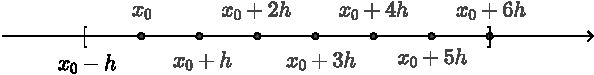
\includegraphics{figures/calculus-rudiments05}.
\par\end{center}

\noindent Untuk stensil ini, $a=x_{0}-h$, $b=x_{0}+6h$, dan $\theta_{i}=ih$,
$i=0,1,\ldots,6$. Dengan demikian, kita akan memperoleh sistem tujuh
persamaan dengan tujuh peubah tak diketahui. Pertama, ruas kirinya:

\begin{eqnarray*}
\int_{a}^{b}p_{0}(x)dx=\int_{x_{0}-h}^{x_{0}+6h}p_{0}(x)dx & = & \int_{x_{0}-h}^{x_{0}+6h}1dx=\left.(x-x_{0})\right|_{x_{0}-h}^{x_{0}+6h}=7h\\
\int_{a}^{b}p_{1}(x)dx=\int_{x_{0}-h}^{x_{0}+6h}p_{1}(x)dx & = & \int_{x_{0}-h}^{x_{0}+6h}(x-x_{0})dx=\left.\frac{1}{2}(x-x_{0})^{2}\right|_{x_{0}-h}^{x_{0}+6h}=\frac{35}{2}h^{2}\\
\int_{a}^{b}p_{2}(x)dx=\int_{x_{0}-h}^{x_{0}+6h}p_{2}(x)dx & = & \int_{x_{0}-h}^{x_{0}+6h}(x-x_{0})^{2}dx=\left.\frac{1}{3}(x-x_{0})^{3}\right|_{x_{0}-h}^{x_{0}+6h}=\frac{217}{3}h^{3}\\
\int_{a}^{b}p_{3}(x)dx=\int_{x_{0}-h}^{x_{0}+6h}p_{3}(x)dx & = & \int_{x_{0}-h}^{x_{0}+6h}(x-x_{0})^{3}dx=\left.\frac{1}{4}(x-x_{0})^{4}\right|_{x_{0}-h}^{x_{0}+6h}=\frac{1295}{4}h^{4}\\
\int_{a}^{b}p_{4}(x)dx=\int_{x_{0}-h}^{x_{0}+6h}p_{4}(x)dx & = & \int_{x_{0}-h}^{x_{0}+6h}(x-x_{0})^{4}dx=\left.\frac{1}{5}(x-x_{0})^{5}\right|_{x_{0}-h}^{x_{0}+6h}=\frac{7777}{5}h^{5}\\
\int_{a}^{b}p_{5}(x)dx=\int_{x_{0}-h}^{x_{0}+6h}p_{5}(x)dx & = & \int_{x_{0}-h}^{x_{0}+6h}(x-x_{0})^{5}dx=\left.\frac{1}{6}(x-x_{0})^{6}\right|_{x_{0}-h}^{x_{0}+6h}=\frac{46655}{6}h^{6}\\
\int_{a}^{b}p_{6}(x)dx=\int_{x_{0}-h}^{x_{0}+6h}p_{6}(x)dx & = & \int_{x_{0}-h}^{x_{0}+6h}(x-x_{0})^{6}dx=\left.\frac{1}{7}(x-x_{0})^{7}\right|_{x_{0}-h}^{x_{0}+6h}=39991h^{7}.
\end{eqnarray*}
Sekarang kita gabungkan semuanya dengan ruas kanan (dan menukar ruas):
\begin{eqnarray*}
\sum_{i=0}^{6}(\theta_{i}h)^{0}a_{i} & = & a_{0}+a_{1}+a_{2}+a_{3}+a_{4}+a_{5}+a_{6}=7h\\
\sum_{i=0}^{6}(\theta_{i}h)^{1}a_{i} & = & ha_{1}+2ha_{2}+3ha_{3}+4ha_{4}+5ha_{5}+6ha_{6}=\frac{35}{2}h^{2}\\
\sum_{i=0}^{6}(\theta_{i}h)^{2}a_{i} & = & h^{2}a_{1}+4h^{2}a_{2}+9h^{2}a_{3}+16h^{2}a_{4}+25h^{2}a_{5}+36h^{2}a_{6}=\frac{217}{3}h^{3}\\
\sum_{i=0}^{6}(\theta_{i}h)^{3}a_{i} & = & h^{3}a_{1}+8h^{3}a_{2}+27h^{3}a_{3}+64h^{3}a_{4}+125h^{3}a_{5}+216h^{3}a_{6}=\frac{1295}{4}h^{4}\\
\sum_{i=0}^{6}(\theta_{i}h)^{4}a_{i} & = & h^{4}a_{1}+16h^{4}a_{2}+81h^{4}a_{3}+256h^{4}a_{4}+625h^{4}a_{5}+1296h^{4}a_{6}=\frac{7777}{5}h^{5}\\
\sum_{i=0}^{6}(\theta_{i}h)^{5}a_{i} & = & h^{5}a_{1}+32h^{5}a_{2}+243h^{5}a_{3}+1024h^{5}a_{4}+3125h^{5}a_{5}+7776h^{5}a_{6}=\frac{46655}{6}h^{6}\\
\sum_{i=0}^{6}(\theta_{i}h)^{6}a_{i} & = & h^{6}a_{1}+64h^{6}a_{2}+729h^{6}a_{3}+4096h^{6}a_{4}+15625h^{6}a_{5}+46656h^{6}a_{6}=39991h^{7}
\end{eqnarray*}
Sekali lagi, sistem ini dapat diselesaikan dengan substitusi, eliminasi,
atau aljabar komputer, setidaknya secara prinsip. Namun, tidak banyak
orang yang memiliki cukup kesabaran dan ketelitian untuk menyelesaikan
sistem seperti itu dengan kertas dan pensil. Dengan mengandalkan sistem
aljabar komputer, penyelesaiannya adalah $a_{0}=\frac{30919}{8640}h$,
$a_{1}=-\frac{2107}{360}h$, $a_{2}=\frac{34153}{2880}h$, $a_{3}=-\frac{1274}{135}h$,
$a_{4}=\frac{19943}{2880}h$, $a_{5}=-\frac{49}{72}h$, dan $a_{6}=\frac{5257}{8640}h$
sehingga diperoleh rumus aproksimasi
\begin{eqnarray}
\int_{x_{0}-h}^{x_{0}+6h}f(x)dx & \approx & \frac{h}{8640}\left[5257f(x_{0}+6h)-5880f(x_{0}+5h)+59829f(x_{0}+4h)-81536f(x_{0}+3h)\right.\nonumber \\
 &  & \qquad\qquad\left.+102459f(x_{0}+2h)-50568f(x_{0}+h)+30919f(x_{0})\right]\label{eq:dumbIntegral7}
\end{eqnarray}
seperti yang telah kita peroleh \vpageref{eq:integral7dumb} dalam
rumus \ref{eq:integral7dumb}.

\subsection{Pertimbangan praktis}

Kita telah menggunakan stensil seperti 

\begin{center}
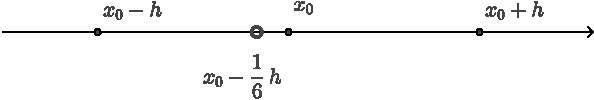
\includegraphics{figures/calculus-rudiments01}
\par\end{center}

\noindent dan 

\begin{center}
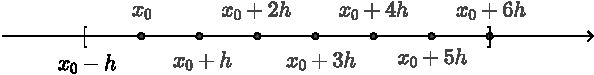
\includegraphics{figures/calculus-rudiments05}
\par\end{center}

\noindent bukan karena hasilnya sangat berguna, melainkan untuk (a)
mengilustrasikan metode tersebut dan (b) menekankan bahwa metode ini
berlaku secara umum untuk setiap stensil yang dapat Anda bayangkan.
Sebagian besar rumus diferensiasi dan integrasi dalam literatur analisis
numerik hanya menggunakan sejumlah kecil stensil berjarak teratur.
Untuk turunan, titik evaluasinya merupakan salah satu simpul; untuk
integral, semua simpul berada di antara kedua batas atau terdapat
simpul pada kedua batas. Mungkin saja hanya stensil berjarak teratur
yang akan Anda perlukan, tetapi ada baiknya mengetahui bahwa Anda
dapat menurunkan rumus yang sesuai untuk stensil yang tidak lazim
jika diperlukan.

Dalam hal penurunannya, keunggulan utama metode koefisien tak tentu
dibandingkan bekerja langsung dengan polinom interpolasi adalah kemudahan
otomasi serta berkurangnya pekerjaan aljabar yang sering kali rumit
dan melelahkan. Dalam metode koefisien tak tentu, satu-satunya polinom
yang perlu diturunkan atau diintegralkan adalah polinom $p_{j}=(x-x_{0})^{j}$,
tugas yang jauh lebih sederhana daripada mengintegralkan atau menurunkan
polinom interpolasi. Rumus dengan tiga atau empat simpul dapat ditangani
dengan cara ini menggunakan pensil dan kertas. Konsekuensinya adalah
perlunya menyelesaikan suatu sistem persamaan, yang sekali lagi lebih
sederhana daripada menurunkan dan menyederhanakan polinom interpolasi
berderajat 3 atau 4. Keunggulan terakhir metode koefisien tak tentu
adalah bahwa metode ini merupakan teknik penyelesaian umum yang tidak
hanya digunakan dalam analisis numerik untuk menurunkan aproksimasi
kalkulus, tetapi juga dalam bidang lain, terutama dalam persamaan
diferensial. Metode ini dapat diterapkan kapan pun \textit{bentuk}
suatu penyelesaian atau rumus diketahui, tetapi konstantanya (koefisien)
masih belum diketahui.

\noindent\begin{digression}{Koefisien Tak Tentu dalam Persamaan Diferensial}

\noindent Dalam persamaan diferensial, kita mengetahui bahwa suatu
solusi khusus dari persamaan
\begin{equation}
y-2y'+3y''=5\sin x\label{eq:differentialEquation}
\end{equation}
berbentuk $y=A\sin x+B\cos x$, tetapi kita belum langsung mengetahui
nilai $A$ dan $B$. Keduanya merupakan koefisien tak tentu (pada
tahap ini). Koefisien tersebut ditentukan dengan menyubstitusikan
bentuk yang diketahui ke dalam persamaan yang sedang diselesaikan.
\begin{eqnarray*}
y' & = & A\cos x-B\sin x\\
y'' & = & -A\sin x-B\cos x
\end{eqnarray*}
Dengan demikian, persamaan yang sedang diselesaikan menjadi
\[
(A\sin x+B\cos x)-2(A\cos x-B\sin x)+3(-A\sin x-B\cos x)=5\sin x.
\]
Dengan mengumpulkan koefisien $\sin x$ dan $\cos x$ pada ruas kiri,
\[
(-2A+2B)\sin x+(-2A-2B)\cos x=5\sin x.
\]
Sekarang kita menyamakan koefisien pada ruas kiri dan kanan untuk
memperoleh sistem persamaan
\begin{eqnarray*}
-2A+2B & = & 5\\
-2A-2B & = & 0
\end{eqnarray*}
yang penyelesaiannya adalah $A=-\frac{5}{4}$ dan $B=\frac{5}{4}$.
Oleh karena itu, $y=-\frac{5}{4}\sin x+\frac{5}{4}\cos x$ merupakan
solusi persamaan \ref{eq:differentialEquation}.

Secara konseptual, proses ini tidak berbeda dari metode koefisien
tak tentu yang digunakan untuk menurunkan rumus kalkulus numerik.
Bentuk penyelesaian suatu masalah telah diketahui, kecuali beberapa
koefisien (yang belum ditentukan). Parameter masalah mengharuskan
koefisien tersebut memenuhi suatu sistem persamaan linear. Sistem
tersebut diselesaikan, sehingga solusi masalah semula akhirnya diketahui
secara lengkap karena koefisiennya telah ditentukan.

\noindent\end{digression}

Ketika kita menggunakan stensil dengan lebih dari 3 atau 4 simpul,
menyelesaikan sistem persamaan linear (yang relatif besar) yang dihasilkan
secara manual bukanlah tugas yang dinantikan oleh kebanyakan dari
kita. Namun, ini merupakan perhitungan standar yang dapat dilakukan
oleh setiap sistem aljabar komputer dengan mudah dan efisien. Memang,
sebaiknya kita menggunakan sistem aljabar komputer untuk menurunkan
rumus serumit \ref{eq:integral7dumb}. Kita telah menggunakan Maxima\footnote{Lihat \url{http://maxima.sourceforge.net/}}\index{Maxima}
untuk menangani atau memeriksa ulang sejumlah perhitungan yang lebih
melelahkan yang disajikan dalam buku ini.

\noindent\begin{digression}{wxMaxima}\index{wxMaxima}\index{Maxima}

\noindent Cara terbaik untuk menyelesaikan sistem persamaan linear
yang besar adalah dengan bantuan sistem aljabar komputer. Gambar \ref{fig:wxMaxima}
menunjukkan cara menggunakan wxMaxima untuk menurunkan rumus \ref{eq:dumbIntegral7}.

Perhatikan kemiripan antara kode Maxima dan kode Octave. Maxima mendukung
pernyataan, pernyataan cetak, penugasan variabel, larik, dan penyembunyian
keluaran. Sintaks untuk hal-hal tersebut tidak sama, tetapi prinsip
yang mendasarinya sama. Setelah Anda mempelajari cara melakukan hal-hal
tersebut dalam satu bahasa, mempelajari caranya dalam bahasa lain
biasanya mudah.

Perhatikan pula perbedaan utama antara Maxima dan Octave. Maxima dirancang
untuk manipulasi simbolik, sedangkan Octave dirancang untuk komputasi
numerik. Octave dapat digunakan untuk melakukan perhitungan simbolik
dan Maxima dapat digunakan untuk melakukan komputasi numerik, tetapi
pepatah lama tukang kayu ``gunakan alat yang tepat untuk pekerjaan
yang dihadapi'' patut dipertimbangkan. Maxima jauh lebih mahir dalam
manipulasi simbolik daripada Octave, sedangkan Octave jauh lebih mahir
dalam mengolah angka daripada Maxima.

\subsection*{Referensi}

\url{http://andrejv.github.io/wxmaxima/}

\noindent\end{digression} 
\begin{figure}
\caption{\label{fig:wxMaxima}Menurunkan rumus integrasi dengan wxMaxima}

\centering{}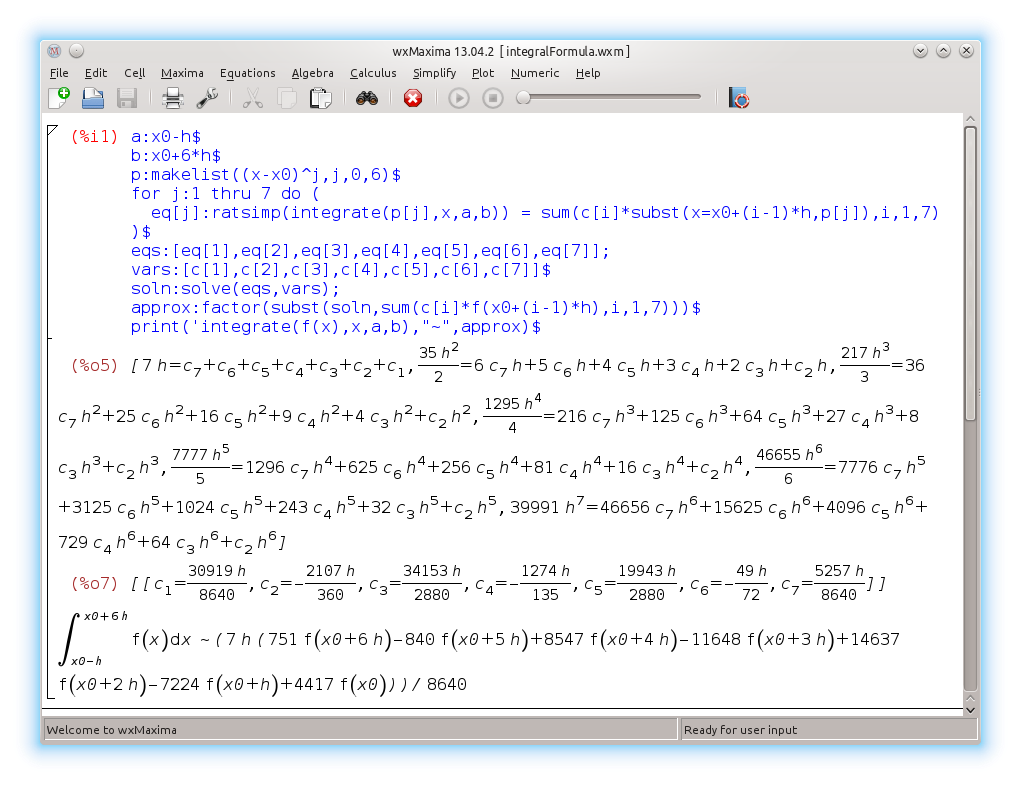
\includegraphics[width=5.5in]{figures/wxmaximaScreenshot}
\end{figure}
 

Pada praktiknya, penggunaan stensil dengan lebih dari lima simpul
memang tidak lazim. Namun, hal ini bukan karena rumus dengan lebih
banyak simpul jauh lebih rumit atau sulit digunakan. Seperti ditunjukkan
oleh rumus \ref{eq:lagrangeInterpolatingPolynomialError}, suku galat
polinom interpolasi melibatkan turunan yang semakin tinggi dari $f$
seiring bertambahnya jumlah simpul. Hal ini umumnya tidak menjadi
masalah selama $f$ memiliki turunan hingga orde yang cukup tinggi
dan nilai turunan berorde tinggi tersebut tidak terlampau besar. Namun,
metode numerik sering digunakan ketika kehalusan $f$ diketahui terbatas,
turunan orde tingginya diketahui bernilai besar, atau sifat-sifat
turunannya sama sekali tidak diketahui. Untuk fungsi-fungsi ini, stensil
dengan lebih sedikit simpul, yang menghasilkan rumus dengan suku galat
berorde lebih rendah, sering kali \textit{lebih akurat}, bukan kurang
akurat. Jika tingkat kehalusannya tidak diketahui, metode berorde
lebih rendah juga memiliki peluang lebih besar untuk tetap akurat.

Sebagai catatan terakhir, kita perlu berhati-hati agar tidak menuntut
terlalu banyak dari suatu rumus turunan. Dengan $n+1$ simpul, suku
galat polinom interpolasi melibatkan $f^{(n+1)}$, sehingga tidak
mungkin menggunakan simpul-simpul ini untuk memperkirakan $f^{(n+1)}$
atau turunan yang lebih tinggi pada titik mana pun. Namun, jika Anda
melupakan fakta ini, hal tersebut akan tampak secara langsung dalam
metode koefisien tak tentu. Jika $k>n$, sistem persamaan dengan koefisien
tak tentu menjadi
\[
\sum_{i=0}^{n}(\theta_{i}h)^{j}a_{i}=0,\qquad j=0,1,\ldots,n
\]
karena turunan orde $k$ dari $p_{j}$ identik nol untuk semua $j\leq n<k$.
Satu-satunya penyelesaian sistem ini adalah $a_{0}=a_{1}=\cdots=a_{n}=0$
sehingga diperoleh rumus ``aproksimasi'' berikut
\[
f^{(k)}(x_{0}+\theta h)=0.
\]
Memang, rumus ini eksak untuk semua polinom berderajat $n$ atau kurang.
Namun, galat akibat penggunaan rumus ini tepat sebesar $f^{(k)}(x_{0}+\theta h)$,
yaitu galat relatif tepat sebesar $1$, sehingga rumus ini sama sekali
tidak berguna.

\subsection{Stabilitas}

Dalam Eksperimen 2 \vpageref{subsec:derivativeExperiment}, bagian
\ref{sec:Accuracy}, kita meninjau secara singkat aproksimasi turunan
pertama $f(x)=\sin x$ dengan menggunakan fakta bahwa
\[
f'(1)=\lim_{h\to0}\frac{\sin(1+h)-\sin(1-h)}{2h}.
\]
Kesimpulan yang kita peroleh adalah bahwa perhitungan ini sangat rentan
terhadap galat titik mengambang. Jika perhitungan dilakukan secara
eksak, kita berharap $\frac{\sin(1+h)-\sin(1-h)}{2h}$ mengaproksimasi
$f'(1)$ dengan semakin baik saat $h$ semakin kecil. Namun, hal ini
tidak berlaku untuk perhitungan titik mengambang, seperti ditunjukkan
oleh eksperimen tersebut. Ada suatu titik ketika memperkecil $h$
justru memperburuk aproksimasi! Contoh ini pun bukan satu-satunya.
Masalah ini selalu muncul ketika mengaproksimasi $f'$ menggunakan
rumus beda terpusat
\begin{equation}
f'(x)\approx\frac{f(x+h)-f(x-h)}{2h}.\label{eq:centeredDifference}
\end{equation}
Namun, bagaimana kita dapat memperkirakan nilai $h$ yang akan memicu
hal itu tanpa membandingkan hasil kita dengan nilai eksak turunannya?
Bagaimanapun, diferensiasi numerik paling sering digunakan ketika
rumus eksak turunannya tidak diketahui atau terlampau sulit untuk
dihitung.

Misalkan $f$ dapat dihitung dengan ketelitian yang mendekati presisi
mesin. Dalam perhitungan titik mengambang biasa, termasuk Octave,
hal itu berarti galat titik mengambang relatif sekitar $10^{-15}$
atau galat titik mengambang mutlak $\varepsilon_{f}\approx10^{-15}|f(x)|$.
Karena kita mengasumsikan $h$ bernilai kecil, kita dapat mengaproksimasi
baik $|\tilde{f}(x+h)-f(x+h)|$ maupun $|\tilde{f}(x-h)-f(x-h)|$
dengan $\varepsilon_{f}$ sehingga diperoleh galat mutlak sekitar
$2\varepsilon_{f}$ dalam menghitung pembilang $f(x+h)-f(x-h)$. Dengan
mengasumsikan $h$ dihitung secara eksak, kita memperoleh galat mutlak
\begin{equation}
\varepsilon_{r}=|\tilde{f}'(x)-f'(x)|\approx\frac{2\varepsilon_{f}}{2h}=\frac{\varepsilon_{f}}{h}=\frac{|f(x)|}{10^{15}}\cdot\frac{1}{h}.\label{eq:floatingPointError}
\end{equation}
Seperti yang akan segera kita lihat, galat algoritmik, $\varepsilon_{a}$,
disebabkan oleh pemotongan dan bernilai $\left|\frac{f'''(\xi)}{6}h^{2}\right|$
untuk suatu nilai $\xi$ di dekat $x$. Karena $\xi$ berada di dekat
$x$, kita mengaproksimasi $f'''(\xi)$ dengan $f'''(x)$ dan menyimpulkan
bahwa 
\begin{equation}
\varepsilon_{a}\approx\frac{|f'''(x)|}{6}h^{2}.\label{eq:algorithmicError}
\end{equation}
Sekarang kita meminimumkan nilai $\varepsilon_{r}+\varepsilon_{a}$
dengan menetapkan turunannya (terhadap $h$) sama dengan nol dan menyelesaikan
persamaan yang dihasilkan:
\begin{eqnarray*}
0=\frac{d}{dh}(\varepsilon_{r}+\varepsilon_{a}) & \approx & \frac{d}{dh}\left(\frac{|f(x)|}{10^{15}}\cdot\frac{1}{h}+\frac{|f'''(x)|}{6}\cdot h^{2}\right)\\
 & = & -\frac{|f(x)|}{10^{15}}\cdot\frac{1}{h^{2}}+\frac{|f'''(x)|}{3}\cdot h\\
 & \Rightarrow\\
\frac{|f'''(x)|}{3}\cdot h & \approx & \frac{|f(x)|}{10^{15}}\cdot\frac{1}{h^{2}}\\
h^{3} & \approx & \frac{|f(x)|}{|f'''(x)|}\cdot\frac{3}{10^{15}}\\
h & \approx & \sqrt[3]{\frac{3|f(x)|}{|f'''(x)|}}\cdot10^{-5}.
\end{eqnarray*}
Untuk Eksperimen 2 \vpageref{subsec:derivativeExperiment}, ini berarti
kita memperkirakan bahwa nilai optimal $h$ berada di sekitar$\sqrt[3]{\frac{3\sin(1)}{\sin(1)}}\cdot10^{-5}\approx1.44(10)^{-5}$.
Kita tampilkan kembali tabel dari Eksperimen 2 di sini dengan menambahkan
kolom ketiga, yaitu galat mutlak sebenarnya:

\begin{center}
\begin{tabular}{c|c|c}
$h$ & $\tilde{p}^{*}(h)$ & $|\tilde{p}^{*}(h)-f'(1)|$\tabularnewline
\hline 
$10^{-2}$ & $0.5402933008747335$ & $9.00(10)^{-6}$\tabularnewline
$10^{-3}$ & $0.5403022158176896$ & $9.00(10)^{-8}$\tabularnewline
$10^{-4}$ & $0.5403023049677103$ & $9.00(10)^{-10}$\tabularnewline
$10^{-5}$ & $0.5403023058569989$ & $1.11(10)^{-11}$\tabularnewline
$10^{-6}$ & $0.5403023058958567$ & $2.77(10)^{-11}$\tabularnewline
$10^{-7}$ & $0.5403023056738121$ & $1.94(10)^{-10}$\tabularnewline
\end{tabular}
\par\end{center}

\noindent Memang, ketika $h=10^{-5}$, kita memperoleh hasil terbaik!
Namun, prediksi nilai optimal untuk $h$ didasarkan pada pengetahuan
tentang $f'''$, sesuatu yang umumnya tidak dapat kita ketahui. Kecuali
jika kebetulan kita mengetahui bahwa $\frac{|f(x)|}{|f'''(x)|}$ jauh
dari $1$, kita mengasumsikan nilainya cukup dekat dengan $1$; dalam
hal ini, nilai optimal $h$ berada di sekitar $10^{-5}$. Perkiraan
serupa dapat dibuat untuk rumus turunan lainnya.

Karena diferensiasi numerik sangat peka terhadap galat titik mengambang,
kita menyebutnya tidak stabil. Metode pencarian akar dan integrasi
numerik yang telah kita bahas semuanya merupakan metode yang stabil.
Kepekaannya terhadap galat titik mengambang sebanding dengan kepekaan
dalam menghitung $f$.

\subsection{Konsep Kunci}
\begin{description}
\item [{koefisien~tak}] tentu: \index{koefisien tak tentu}Metode untuk
menyelesaikan masalah yang bentuk penyelesaiannya telah diketahui,
kecuali sejumlah koefisien yang belum ditentukan.
\end{description}
\noindent\startexercises 

\subsection{Latihan}
\begin{enumerate}
\item \label{exc:undetermined}Dengan menggunakan metode koefisien tak tentu,
turunkan rumus aproksimasi untuk turunan pertama pada stensil tersebut.

\begin{enumerate}
\item \raisepic{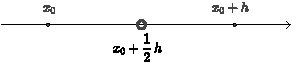
\includegraphics{figures/calculus-undetermined01}}\medskip 
\item \raisepic{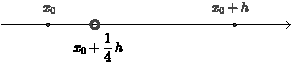
\includegraphics{figures/calculus-undetermined06}} \hasananswer\medskip 
\item \raisepic{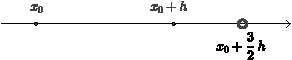
\includegraphics{figures/calculus-undetermined07}}\medskip 
\item \raisepic{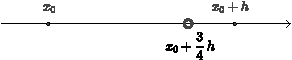
\includegraphics{figures/calculus-undetermined08}} \hasasolution\medskip 
\item \raisepic{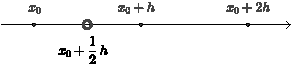
\includegraphics{figures/calculus-undetermined02}}\medskip 
\item \raisepic{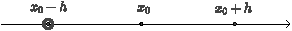
\includegraphics{figures/calculus-undetermined03}} \hasananswer\medskip 
\item \raisepic{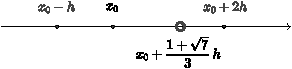
\includegraphics{figures/calculus-undetermined04}}\medskip 
\item \raisepic{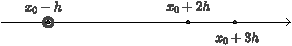
\includegraphics[width=5cm]{figures/calculus-undetermined05}} \hasananswer\medskip 
\item \raisepic{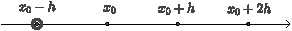
\includegraphics{figures/calculus-undetermined09}}\medskip 
\item \raisepic{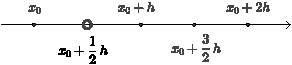
\includegraphics{figures/calculus-undetermined10}} \hasasolution\medskip 
\item \raisepic{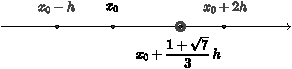
\includegraphics{figures/calculus-undetermined11}}\medskip 
\item \raisepic{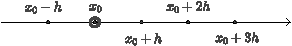
\includegraphics{figures/calculus-undetermined12}} \hasananswer
\end{enumerate}
\item \label{exc:undetermined-1}Dengan menggunakan metode koefisien tak
tentu, turunkan rumus aproksimasi untuk turunan kedua pada stensil
tersebut.

\begin{enumerate}
\item \raisepic{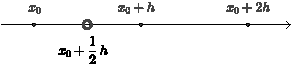
\includegraphics{figures/calculus-undetermined02}}\medskip 
\item \raisepic{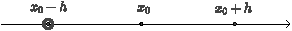
\includegraphics{figures/calculus-undetermined03}} \hasananswer\medskip 
\item \raisepic{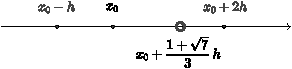
\includegraphics{figures/calculus-undetermined04}}\medskip 
\item \raisepic{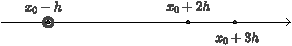
\includegraphics[width=5cm]{figures/calculus-undetermined05}} \hasananswer\medskip 
\item \raisepic{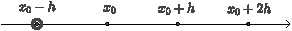
\includegraphics{figures/calculus-undetermined09}}\medskip 
\item \raisepic{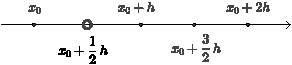
\includegraphics{figures/calculus-undetermined10}} \hasasolution\medskip 
\item \raisepic{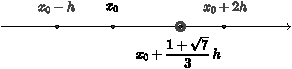
\includegraphics{figures/calculus-undetermined11}}\medskip 
\item \raisepic{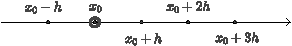
\includegraphics{figures/calculus-undetermined12}} \hasananswer 
\end{enumerate}
\item Gunakan metode koefisien tak tentu untuk menurunkan rumus aproksimasi
pada stensil berikut

\begin{center}
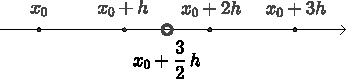
\includegraphics{figures/calculus-rudiments07}
\par\end{center}
\begin{enumerate}
\item untuk nilai fungsi.
\item untuk turunan pertama.
\item untuk turunan kedua.
\item untuk turunan ketiga. Apa yang dapat Anda simpulkan tentang rumus
ini?
\item Bandingkan metode koefisien tak tentu dengan metode langsung yang
digunakan pada soal \ref{exc:rudiments-28} di bagian \ref{sec:NumericalRudiments}.
\end{enumerate}
\item \label{exc:undetermined-2}Gunakan metode koefisien tak tentu untuk
menurunkan rumus aproksimasi untuk integral pada stensil berikut.

\begin{enumerate}
\item \raisepic{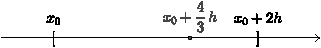
\includegraphics{figures/calculus-undetermined13}}\medskip
\item \raisepic{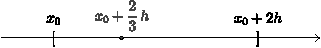
\includegraphics{figures/calculus-undetermined14}} \hasasolution\medskip
\item \raisepic{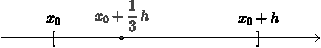
\includegraphics{figures/calculus-undetermined15}}\medskip
\item \raisepic{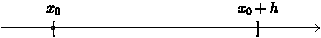
\includegraphics{figures/calculus-undetermined16}} \hasananswer\medskip
\item \raisepic{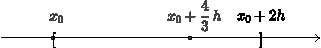
\includegraphics{figures/calculus-rudiments16}}\medskip
\item \raisepic{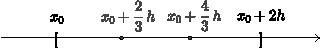
\includegraphics{figures/calculus-rudiments17}} \hasananswer\medskip
\item \raisepic{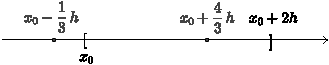
\includegraphics{figures/calculus-rudiments19}}\medskip
\item \raisepic{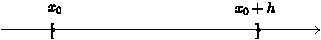
\includegraphics{figures/calculus-rudiments20}} \hasananswer\medskip
\item \raisepic{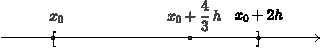
\includegraphics{figures/calculus-undetermined17}}\medskip
\item \raisepic{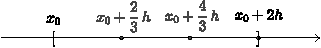
\includegraphics{figures/calculus-undetermined18}} \hasananswer\medskip
\item \raisepic{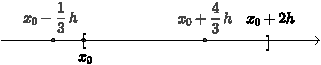
\includegraphics{figures/calculus-undetermined19}}\medskip
\item \raisepic{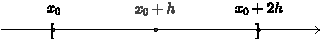
\includegraphics{figures/calculus-undetermined20}} \hasasolution\medskip
\item \raisepic{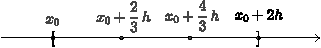
\includegraphics{figures/calculus-undetermined21}}
\end{enumerate}
\item Dengan menggunakan metode koefisien tak tentu, tentukan rumus aproksimasi
umum untuk ${\displaystyle \int_{x_{0}+\theta_{0}h}^{x_{0}+\theta_{1}h}f(x)dx}$
dengan menggunakan dua simpul $x_{0}+\theta_{2}h$ dan $x_{0}+\theta_{3}h$.
\end{enumerate}
\noindent\finishexercises 



\section{\label{sec:calculusErrorAnalysis}Analisis Galat}

\subsection{Galat pada Rumus Turunan Pertama}

Pada bagian \ref{sec:polynomialLagrange}, kita memperoleh bahwa jika
$f$ memiliki turunan yang cukup, maka selisih antara $f$ dan $P_{n}$,
yaitu polinom interpolasi berderajat paling tinggi $n$, diberikan
oleh persamaan \ref{eq:lagrangeInterpolatingPolynomialError} \vpageref{eq:lagrangeInterpolatingPolynomialError},
yang disalin di sini untuk memudahkan:
\[
f(x)-P_{n}(x)=\frac{f^{(n+1)}(\xi_{x})}{(n+1)!}(x-x_{0})(x-x_{1})\cdots(x-x_{n}).
\]
Kita dapat menggunakan rumus ini untuk menurunkan rumus ringkas bagi
galat dalam menghampiri $f'(x)$ dengan $P_{n}'(x)$.

Seperti yang dilakukan pada bagian \ref{sec:polynomialLagrange},
misalkan $n\geq1$ dan $x_{0},x_{1},\ldots,x_{n}$ berjumlah $n$
ditambah satu dan semuanya merupakan bilangan real yang berbeda. Tetapkan
$w(x)=(x-x_{0})(x-x_{1})\cdots(x-x_{n})$, $a=\min(x_{0},\ldots,x_{n},x)$,
serta $b=\max(x_{0},\ldots,x_{n},x)$. Dari persamaan \ref{eq:lagrangeInterpolatingPolynomialError},
kita mengetahui bahwa, dengan mengasumsikan $f$ memiliki $n+1$ turunan
pada $(a,b)$ dan $f',f'',\ldots,f^{(n)}$ semuanya kontinu pada $[a,b]$,
untuk setiap $x\in[a,b]$, berlaku

\[
f(x)-P_{n}(x)=\frac{f^{(n+1)}(\xi_{x})}{(n+1)!}w(x)
\]
untuk suatu $\xi_{x}\in(a,b)$. Oleh karena itu,
\[
f'(x)-P_{n}'(x)=\frac{d}{dx}\left[\frac{f^{(n+1)}(\xi_{x})}{(n+1)!}\right]w(x)+\frac{f^{(n+1)}(\xi_{x})}{(n+1)!}w'(x).
\]
Karena $w$ bernilai nol di setiap simpul, rumus ini menjadi lebih
sederhana ketika $x$ merupakan simpul. Tanpa mengurangi keumuman,
kita mengevaluasinya pada $x=x_{0}$ dan memperoleh 
\[
f'(x_{0})-P_{n}'(x_{0})=\frac{f^{(n+1)}(\xi_{x_{0}})}{(n+1)!}w'(x_{0}).
\]
Mulai dari sini, rumus galat ini hanya berlaku pada sebuah simpul!
Ungkapan terakhir ini dapat disederhanakan lebih lanjut dengan memperhatikan
bahwa 
\[
w'(x)=\sum_{i=0}^{n}\prod_{\substack{j=0\\
i\neq j
}
}^{n}(x-x_{j})=\sum_{i=0}^{n}p_{i}(x),
\]
dengan $p_{i}$ sebagaimana didefinisikan untuk persamaan \ref{eq:lagrangeInterpolatingPolynomial}
\vpageref{eq:lagrangeInterpolatingPolynomial}. Namun, $p_{i}(x_{0})=0$
untuk semua $i$ kecuali $i=0$, sehingga
\[
w'(x_{0})=p_{0}(x_{0})=(x_{0}-x_{1})(x_{0}-x_{2})\cdots(x_{0}-x_{n}).
\]
Dengan menyubstitusikan ungkapan untuk $w'$ ini, kita memperoleh
rumus galat turunan pertama
\[
f'(x_{0})-P_{n}'(x_{0})=\frac{f^{(n+1)}(\xi_{x_{0}})}{(n+1)!}(x_{0}-x_{1})(x_{0}-x_{2})\cdots(x_{0}-x_{n}).
\]
Lakukan substitusi $x_{0}+\theta_{i}h$ untuk $x_{i}$, $i=1,2,\ldots,n$,
agar diperoleh rumus dalam bentuk $h$ dan $\theta_{i}$:
\[
f'(x_{0})-P_{n}'(x_{0})=\frac{f^{(n+1)}(\xi_{x_{0}})}{(n+1)!}(-\theta_{1}h)(-\theta_{2}h)\cdots(-\theta_{n}h).
\]
Rumus galat ini masih dapat sedikit disederhanakan:
\begin{equation}
f'(x_{0})-P_{n}'(x_{0})=\frac{f^{(n+1)}(\xi)}{(n+1)!}\theta_{1}\theta_{2}\cdots\theta_{n}(-h)^{n}.\label{eq:firstDerivErrorSimplified}
\end{equation}

Untuk stensil

\begin{center}
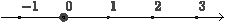
\includegraphics[scale=2]{figures/calculus-errors07},
\par\end{center}

\noindent$n=4$, $\theta_{1}=-1$, $\theta_{2}=1$, $\theta_{3}=2$,
dan $\theta_{4}=3$, sehingga galat dalam menghitung $f'$ pada stensil
ini adalah
\[
\frac{f^{(5)}(\xi)}{120}(-1)(1)(2)(3)(-h)^{4}=-\frac{f^{(5)}(\xi)}{20}h^{4}.
\]
Suku-suku galat untuk turunan pertama pada stensil lain dihitung dengan
cara serupa, asalkan turunannya dievaluasi di sebuah simpul. Tabel
\ref{tab:firstDerivativeFormulas} merangkum beberapa rumus turunan
pertama yang umum, termasuk suku galatnya.

Perhatikan bahwa suku galat memuat $(x_{0}-x_{1})(x_{0}-x_{2})\cdots(x_{0}-x_{n})$
sebagai faktor, yaitu hasil kali semua selisih antara titik evaluasi
dan simpul-simpul lainnya. Jika selisih antara titik evaluasi dan
simpul-simpul lain kecil, hasil kalinya juga kecil. Oleh karena itu,
rumus hampiran turunan pertama umumnya lebih akurat bila titik evaluasi
terletak di tengah di antara simpul-simpul. Dengan demikian, kita
dapat memperkirakan bahwa rumus turunan pertama yang melibatkan simpul
$x_{0}<x_{1}<x_{2}$ akan lebih akurat ketika titik evaluasinya $x_{1}$
daripada ketika titik evaluasinya $x_{0}$ atau $x_{2}$. Hal yang
sama berlaku untuk rumus turunan orde lebih tinggi. Semakin dekat
titik evaluasi ke tengah, semakin akurat hampirannya.

\subsection{Galat pada Rumus Lain\label{subsec:derivativeError}}

Kita mungkin tergoda untuk berpikir bahwa kita cukup mengulangi prosedur
yang digunakan untuk turunan pertama, dengan mengambil turunan kedua
dari $f(x)-P_{n}(x)=\frac{f^{(n+1)}(\xi_{x})}{(n+1)!}w(x)$ untuk
menemukan galat pada taksiran turunan kedua, dan turunan ketiga dari
$f(x)-P_{n}(x)=\frac{f^{(n+1)}(\xi_{x})}{(n+1)!}w(x)$ untuk menemukan
galat pada taksiran turunan ketiga, dan seterusnya. Sayangnya, masalahnya
tidak sesederhana itu. Turunan orde lebih tinggi dari $f(x)-P_{n}(x)=\frac{f^{(n+1)}(\xi_{x})}{(n+1)!}w(x)$
melibatkan turunan dari faktor $\frac{f^{(n+1)}(\xi_{x})}{(n+1)!}$
yang tidak bernilai nol bahkan ketika $x$ merupakan simpul. Karena
$\xi_{x}$ sama sekali tidak diketahui, turunannya pun tidak diketahui
sehingga pendekatan ini tidak dapat digunakan.

Namun, ada metode umum untuk menentukan suku galat yang \textit{cukup
baik} bagi sembarang rumus turunan maupun integral. Setiap evaluasi
$f$ dalam hampiran kita ganti dengan deret Taylor yang dikembangkan
di sekitar $x_{0}$ lalu kita sederhanakan. Ini menghasilkan ungkapan
bagi hampiran dalam bentuk $f(x_{0})$, $f'(x_{0})$, $f''(x_{0})$,
dan seterusnya. Kita membandingkan ungkapan itu dengan representasi
deret Taylor dari besaran yang ditaksir. Selisih keduanya adalah galat.
Ringkasnya, hanya itu. Menyusun argumen yang ketat bagi metode ini
memerlukan kehati-hatian dan layak dibahas melalui sebuah contoh.
Kita memperagakan metode ini untuk hampiran turunan pertama pada stensil

\begin{center}
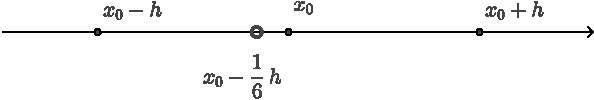
\includegraphics{figures/calculus-rudiments01}.
\par\end{center}

\noindent Sekali lagi, kita memilih stensil ini bukan karena stensil
tersebut berguna secara umum, melainkan untuk menekankan bahwa \textit{metodenya}
berguna secara umum. 

Pada subbagian \ref{subsec:Derivatives} \vpageref{subsec:Derivatives},
kita menurunkan hampiran
\begin{equation}
f'\left(x_{0}-\frac{1}{6}h\right)\approx\frac{-2f(x_{0}-h)+f(x_{0})+f(x_{0}+h)}{3h}.\label{eq:generalApprox}
\end{equation}
Ruas kiri, yaitu besaran yang dihampiri, dalam bentuk deret Taylor
adalah
\[
f'\left(x_{0}-\frac{1}{6}h\right)=f'(x_{0})-\frac{1}{6}hf''(x_{0})+\frac{1}{72}h^{2}f'''(x_{0})-\frac{1}{1296}h^{3}f^{(4)}(x_{0})+\cdots.
\]
Suku-suku pada ruas kanan, yaitu hampirannya, dalam bentuk deret Taylor
adalah
\begin{eqnarray*}
f(x_{0}-h) & = & f(x_{0})-hf'(x_{0})+\frac{1}{2}h^{2}f''(x_{0})-\frac{1}{6}h^{3}f'''(x_{0})+\frac{1}{24}h^{4}f^{(4)}(x_{0})-\cdots\\
f(x_{0}) & = & f(x_{0})\\
f(x_{0}+h) & = & f(x_{0})+hf'(x_{0})+\frac{1}{2}h^{2}f''(x_{0})+\frac{1}{6}h^{3}f'''(x_{0})+\frac{1}{24}h^{4}f^{(4)}(x_{0})+\cdots.
\end{eqnarray*}
Sekarang kita menyubstitusikan deret-deret Taylor ini ke ruas kanan
persamaan \ref{eq:generalApprox} lalu menyederhanakannya. Untuk memudahkan
aljabar, kita mulai dengan menjumlahkan $-2f(x_{0}-h)+f(x_{0})+f(x_{0}+h)$:

\begin{center}
\begin{tabular}{rcl}
$-2f(x_{0}-h)$ & $=$ & $-2f(x_{0})+2hf'(x_{0})-h^{2}f''(x_{0})+\frac{1}{3}h^{3}f'''(x_{0})-\frac{1}{12}h^{4}f^{(4)}(x_{0})-\cdots$\tabularnewline
$f(x_{0})$ & $=$ & $f(x_{0})$\tabularnewline
$f(x_{0}+h)$ & $=$ & $f(x_{0})+hf'(x_{0})+\frac{1}{2}h^{2}f''(x_{0})+\frac{1}{6}h^{3}f'''(x_{0})+\frac{1}{24}h^{4}f^{(4)}(x_{0})+\cdots$\tabularnewline
\hline 
$-2f(x_{0}-h)+f(x_{0})+f(x_{0}+h)$ & $=$ & $3hf'(x_{0})-\frac{1}{2}h^{2}f''(x_{0})+\frac{1}{2}h^{3}f'''(x_{0})-\frac{1}{24}h^{4}f^{(4)}(x_{0})+\cdots$.\tabularnewline
\end{tabular}
\par\end{center}

\noindent Dengan demikian, kita memperoleh 
\begin{eqnarray*}
\frac{-2f(x_{0}-h)+f(x_{0})+f(x_{0}+h)}{3h} & = & \frac{3hf'(x_{0})-\frac{1}{2}h^{2}f''(x_{0})+\frac{1}{2}h^{3}f'''(x_{0})-\frac{1}{24}h^{4}f^{(4)}(x_{0})+\cdots}{3h}\\
 & = & f'(x_{0})-\frac{1}{6}hf''(x_{0})+\frac{1}{6}h^{2}f'''(x_{0})-\frac{1}{72}h^{3}f^{(4)}(x_{0})+\cdots.
\end{eqnarray*}
Untuk galat, $e(h)=f'\left(x_{0}-\frac{1}{6}h\right)-\frac{-2f(x_{0}-h)+f(x_{0})+f(x_{0}+h)}{3h}$,
selanjutnya kita peroleh

\[
\begin{gathered}\left(f'(x_{0})-\frac{1}{6}hf''(x_{0})+\frac{1}{72}h^{2}f'''(x_{0})-\frac{1}{1296}h^{3}f^{(4)}(x_{0})+\cdots\right)\\
\qquad-\left(f'(x_{0})-\frac{1}{6}hf''(x_{0})+\frac{1}{6}h^{2}f'''(x_{0})-\frac{1}{72}h^{3}f^{(4)}(x_{0})+\cdots\right)\\
=-\frac{11}{72}h^{2}f'''(x_{0})+\frac{17}{1296}h^{3}f^{(4)}(x_{0})+\cdots.\qquad\qquad\qquad\qquad\qquad
\end{gathered}
\]
Sebelum melanjutkan, kita perlu membahas notasi O besar\index{O besar}
dalam konteks ini. \index{kekonvergenan!laju} Untuk fungsi $g(h)$
yang memenuhi ${\displaystyle \lim_{h\to0}g(h)=0}$, $p(h)=O(g(h))$
berarti bahwa $|p(h)|\leq M|g(h)|$ untuk suatu konstanta $M$ dan
$h$ yang cukup kecil. Dengan kata lain, besar $p(h)$ dibatasi oleh
besar suatu kelipatan konstan dari $g(h)$. Bandingkan dengan penggunaan
notasi O besar dalam konteks barisan konvergen pada bagian \ref{sec:Speed}. 

Dalam situasi ini, perhitungan kita menunjukkan bahwa galat berbentuk
$O(h^{2}f'''(\xi_{h}))$, yaitu bentuk suku tersisa dengan pangkat
paling rendah. Artinya, $|e(h)|\leq M|h^{2}f'''(\xi_{h})|$ untuk
suatu konstanta $M$ dan $h$ yang cukup kecil, tetapi kita belum
memiliki bukti yang ketat untuk fakta tersebut. Anggaplah apa yang
telah dilakukan sejauh ini sebagai tahap penemuan.

Sekarang kita perlu membuktikan bahwa terdapat $M$ sedemikian rupa
sehingga $|e(h)|\leq M|h^{2}f'''(\xi_{h})|$ berlaku untuk $h$ yang
cukup kecil. Dari perhitungan di atas kita tahu bahwa suku-suku $f'''$
tidak saling meniadakan, jadi kita kembali dan memotong semua deret
Taylor setelah suku $f''$, mengganti turunan berorde lebih tinggi
dengan suku galat, lalu ``mengulang'' aljabarnya. Dengan demikian,
kita mempunyai
\begin{eqnarray*}
f'\left(x_{0}-\frac{1}{6}h\right) & = & f'(x_{0})-\frac{1}{6}hf''(x_{0})+\frac{1}{72}h^{2}f'''(\xi_{1})\\
f(x_{0}-h) & = & f(x_{0})-hf'(x_{0})+\frac{1}{2}h^{2}f''(x_{0})-\frac{1}{6}h^{3}f'''(\xi_{2})\\
f(x_{0}) & = & f(x_{0})\\
f(x_{0}+h) & = & f(x_{0})+hf'(x_{0})+\frac{1}{2}h^{2}f''(x_{0})+\frac{1}{6}h^{3}f'''(\xi_{3})
\end{eqnarray*}
dengan $\xi_{1}\in(x_{0}-\frac{1}{6}h,x_{0})$, $\xi_{2}\in(x_{0}-h,x_{0})$,
serta $\xi_{3}\in(x_{0},x_{0}+h)$. Ketika sekarang kita menghitung
$e(h)=f'\left(x_{0}-\frac{1}{6}h\right)-\frac{-2f(x_{0}-h)+f(x_{0})+f(x_{0}+h)}{3h}$,
kita tahu bahwa semua suku yang melibatkan $f$, $f'$, serta $f''$
saling meniadakan. Hanya suku yang melibatkan $f'''$ yang tersisa:
\begin{eqnarray*}
e(h) & = & \frac{1}{72}h^{2}f'''(\xi_{1})-\frac{-2(-\frac{1}{6}h^{3}f'''(\xi_{2}))+\frac{1}{6}h^{3}f'''(\xi_{3})}{3h}\\
 & = & \frac{1}{72}h^{2}f'''(\xi_{1})-\frac{1}{9}h^{2}f'''(\xi_{2})-\frac{1}{18}h^{2}f'''(\xi_{3})\\
 & = & \frac{h^{2}}{9}\left[\frac{1}{8}f'''(\xi_{1})-f'''(\xi_{2})-\frac{1}{2}f'''(\xi_{3})\right].
\end{eqnarray*}
Langkah formal terakhir adalah mengubah ungkapan ini ke notasi O besar:
\begin{eqnarray*}
|e(h)| & = & \left|\frac{h^{2}}{9}\left[\frac{1}{8}f'''(\xi_{1})-f'''(\xi_{2})-\frac{1}{2}f'''(\xi_{3})\right]\right|\\
 & \leq & \frac{h^{2}}{9}\left[\left|\frac{1}{8}f'''(\xi_{1})\right|+\left|f'''(\xi_{2})\right|+\left|\frac{1}{2}f'''(\xi_{3})\right|\right]\\
 & \leq & \frac{h^{2}}{9}\cdot\frac{13}{8}\max\left\{ \left|f'''(\xi_{1})\right|,\left|f'''(\xi_{2})\right|,\left|f'''(\xi_{3})\right|\right\} \\
 & = & h^{2}\cdot M\left|f'''(\xi_{h})\right|
\end{eqnarray*}
 untuk suatu $\xi_{h}\in(x_{0}-h,x_{0}+h)$ dan $M=\frac{13}{72}$.
Nilai $\xi_{h}$ adalah $\xi_{1}$, $\xi_{2}$, atau $\xi_{3}$. Kita
menyimpulkan
\[
e(h)=O(h^{2}f'''(\xi_{h})).
\]
Secara umum, $\xi_{h}$ dijamin berada di antara simpul terkecil
dan simpul terbesar. Dalam kasus hampiran integral, titik-titik ujung
integrasi diperlakukan sebagai simpul untuk menentukan letak $\xi_{h}$.
Perhatikan bahwa seluruh perhitungan ini bergantung pada kekontinuan
$f'''(x)$ pada interval antara simpul terkecil dan simpul terbesar.
Tanpa kekontinuan tersebut, teorema Taylor tidak berlaku dan semua
perhitungan setelah ekspansi tidak bermakna.

\subsection{Kuadratur Gauss\index{kuadratur!Gauss}}

Pada akhirnya, keakuratan suatu rumus kalkulus numerik diukur melalui
suku galatnya, suatu besaran berbentuk $O(h^{n}f^{(k)}(\xi_{h}))$.
Jika yang kita perhatikan adalah laju kekonvergenan, kita meninjau
$n$, yaitu pangkat $h$ yang muncul dalam suku galat. Semakin besar
pangkat tersebut, semakin cepat kekonvergenannya. Namun, jika yang
kita perhatikan adalah kelas polinom terbesar yang membuat rumus itu
eksak, kita perlu meninjau nilai $k$, yaitu orde turunan yang muncul
dalam suku galat. Semakin besar $k$, semakin besar pula kelas polinom
yang membuat rumus tersebut eksak. Bahkan, jika suku galat memuat
faktor $f^{(k)}(\xi_{h})$, maka rumus tersebut eksak untuk semua
polinom hingga dan termasuk derajat $k-1$. Implikasi lanjutannya
adalah terdapat polinom berderajat $k$ yang untuknya rumus tersebut
tidak eksak, sebab jika tidak demikian, suku galat akan melibatkan
turunan berorde lebih tinggi. Nilai $k-1$ ini kita sebut derajat
ketelitian. Secara formal, derajat ketelitian\index{derajat ketelitian|see\{ketelitian ! derajat\}}\index{ketelitian!derajat}
suatu rumus kalkulus numerik adalah bilangan bulat $m$ sedemikian
rupa sehingga rumus tersebut eksak untuk semua polinom hingga dan
termasuk derajat $m$ tetapi tidak eksak untuk semua polinom berderajat
$m+1$. Rumus kuadratur Gauss bertujuan memaksimalkan derajat ketelitian
rumus integral. 

Turunan dan integral numerik pada stensil dengan $n+1$ titik yang
telah kita turunkan sejauh ini eksak untuk semua polinom hingga derajat
$n$, sebagaimana mestinya. Derajat ketelitiannya sekurang-kurangnya
$n$. Ternyata, beberapa di antaranya memiliki derajat ketelitian
lebih besar daripada $n$. Pertimbangkan hampiran turunan kedua pada
stensil

\begin{center}
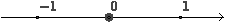
\includegraphics[scale=1.5]{figures/calculus-errors01}.
\par\end{center}

\noindent Stensil ini memiliki tiga titik, jadi kita mengharapkannya
eksak untuk semua polinom hingga derajat 2 (dan memang demikian).
Namun, suku galatnya adalah $O(h^{2}f^{(4)}(\xi_{h}))$, yang menunjukkan
bahwa rumus tersebut eksak untuk semua polinom hingga derajat 3. Jadi,
derajat ketelitiannya sebenarnya 3, bukan 2. Rumus turunan pertama
pada stensil yang sama juga serupa. Walaupun suku galatnya adalah
$\frac{h^{2}}{6}f'''(\xi_{h})$, yang menunjukkan bahwa rumus tersebut
memiliki derajat ketelitian 2 sesuai harapan, rumus itu sendiri hanya
melibatkan dua dari tiga titik yang tersedia! Koefisien $f(x_{0})$
ternyata nol. Dengan demikian, rumus yang sama dapat kita turunkan
dengan menggunakan stensil

\begin{center}
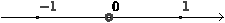
\includegraphics[scale=1.5]{figures/calculus-errors26},
\par\end{center}

\noindent yang hanya memiliki dua titik, tetapi berderajat ketelitian
2. Beberapa beda terpusat lainnya memiliki sifat ini. Rumus Newton-Cotes
dengan jumlah simpul ganjil juga memiliki sifat ini. Derajat ketelitiannya
melampaui perkiraan sebesar satu derajat. Sebelumnya kita mencatat
bahwa titik evaluasi yang terletak di tengah cenderung meningkatkan
keakuratan, dan sekarang kita melihat bahwa peningkatan itu dapat
sangat besar.

Dari pengamatan ini dapat kita simpulkan bahwa bukan hanya jumlah
simpul yang menentukan suku galat suatu rumus kalkulus numerik. Letak
simpul juga penting. Sampai saat ini, kita baru melihat bagaimana
letak simpul memengaruhi hampiran turunan. Kita tahu bahwa menempatkan
titik evaluasi di tengah pada umumnya meningkatkan keakuratan. Sekarang
kita membahas cara menempatkan simpul untuk meningkatkan keakuratan
rumus integral. Namun, gagasan titik evaluasi yang berada di tengah
tidak bermakna dalam konteks ini. Integral tidak memiliki satu titik
evaluasi; integral dihitung pada suatu interval. Yang penting adalah
letak simpul relatif terhadap titik-titik ujung integrasi. Sekarang
kita akan menentukan letak simpul agar derajat ketelitian terbesar
tercapai untuk setiap jumlah simpul tertentu.

Misalkan $G_{n}$ adalah polinom Legendre ke-$n$, yang didefinisikan
secara rekursif oleh 
\begin{eqnarray*}
G_{n+1}(x) & = & \frac{(2n+1)xG_{n}(x)-nG_{n-1}(x)}{n+1}\\
G_{0}(x) & = & 1\\
G_{1}(x) & = & x.
\end{eqnarray*}
Kita menetapkan $\theta_{i}$ sama dengan akar-akar $G_{n}$ untuk
menurunkan rumus kuadratur $n$-titik pada interval $[x_{0}-h,x_{0}+h]$
dengan derajat ketelitian terbesar yang mungkin. Setelah penempatan
simpul dipilih, kita memaksa rumus tersebut eksak bagi polinom hingga
derajat $n-1$, seperti yang kita lakukan sebelumnya. Perbedaannya
kali ini adalah bahwa karena nilai khusus $\theta_{i}$, rumus yang
dihasilkan akan eksak untuk semua polinom hingga derajat $2n-1$.
Ketika simpul ditempatkan pada akar-akar polinom Legendre ke-$n$,
kita memperoleh rumus kuadratur untuk $\int_{x_{0}-h}^{x_{0}+h}f(x)dx$
yang melampaui derajat ketelitian yang diharapkan sebesar $n$, yaitu
jumlah simpul!

Kita memperagakannya untuk $n=1$ dan $n=3$.

\[
G_{1}(x)=x
\]
memiliki satu-satunya akar, $0$. Oleh karena itu, kita mencari rumus
berbentuk 
\[
\int_{x_{0}-h}^{x_{0}+h}f(x)dx\approx a_{0}f(x_{0})
\]
yang eksak untuk polinom hingga derajat $0$. Persamaan tunggal untuk
satu peubah tak diketahui, $a_{0}$, adalah
\[
\int_{x_{0}-h}^{x_{0}+h}(1)dx=a_{0}(1)
\]
atau $2h=a_{0}$. Oleh karena itu, kita memperoleh
\[
\int_{x_{0}-h}^{x_{0}+h}f(x)dx\approx2hf(x_{0}),
\]
yang kita klaim berderajat ketelitian 1, bukan 0. Memang, untuk $f(x)=x-x_{0}$,
\[
\int_{x_{0}-h}^{x_{0}+h}f(x)dx=\left.\frac{1}{2}(x-x_{0})^{2}\right|_{x_{0}-h}^{x_{0}+h}=0
\]
 dan
\[
2hf(x_{0})=2h(x_{0}-x_{0})=0,
\]
sehingga rumus tersebut eksak untuk polinom berderajat satu. Namun,
untuk $f(x)=(x-x_{0})^{2}$,
\[
\int_{x_{0}-h}^{x_{0}+h}f(x)dx=\left.\frac{1}{3}(x-x_{0})^{3}\right|_{x_{0}-h}^{x_{0}+h}=\frac{2}{3}h^{3}
\]
tetapi
\[
2hf(x_{0})=2h(x_{0}-x_{0})^{2}=0,
\]
sehingga rumus tersebut tidak eksak untuk semua polinom berderajat
dua. Jadi, derajat ketelitiannya adalah 1. Perhatikan bahwa rumus
${\displaystyle \int_{x_{0}-h}^{x_{0}+h}f(x)dx\approx2hf(x_{0})}$
setara dengan Aturan Titik Tengah seperti yang tercantum pada Tabel
\ref{tab:integrationFormulas}.

Sekarang
\begin{eqnarray*}
G_{2}(x) & = & \frac{3xG_{1}(x)-G_{0}(x)}{2}\\
 & = & \frac{1}{2}(3x^{2}-1)
\end{eqnarray*}
 sehingga
\begin{eqnarray*}
G_{3}(x) & = & \frac{5xG_{2}(x)-2G_{1}(x)}{3}\\
 & = & \frac{\frac{5}{2}(3x^{3}-x)-2x}{3}\\
 & = & \frac{5(3x^{3}-x)-4x}{6}\\
 & = & \frac{15x^{3}-9x}{6}\\
 & = & \frac{1}{2}(5x^{3}-3x),
\end{eqnarray*}
yang memiliki akar-akar $-\sqrt{\frac{3}{5}},0,\sqrt{\frac{3}{5}}$.
Oleh karena itu, kita mencari rumus berbentuk 
\[
\int_{x_{0}-h}^{x_{0}+h}f(x)dx\approx a_{0}f\left(x_{0}-\sqrt{\frac{3}{5}}h\right)+a_{1}f(x_{0})+a_{2}f\left(x_{0}+\sqrt{\frac{3}{5}}h\right)
\]
yang eksak untuk polinom hingga derajat $2$. Tiga persamaan untuk
tiga peubah tak diketahui tersebut adalah
\begin{eqnarray*}
\int_{x_{0}-h}^{x_{0}+h}(1)dx=2h & = & a_{0}+a_{1}+a_{2}\\
\int_{x_{0}-h}^{x_{0}+h}(x-x_{0})dx=0 & = & -\sqrt{\frac{3}{5}}ha_{0}+\sqrt{\frac{3}{5}}ha_{2}\\
\int_{x_{0}-h}^{x_{0}+h}(x-x_{0})^{2}dx=\frac{2}{3}h^{3} & = & \frac{3}{5}h^{2}a_{0}+\frac{3}{5}h^{2}a_{2}.
\end{eqnarray*}
Solusinya adalah 
\[
a_{0}=a_{2}=\frac{5}{9}h\quad\mbox{dan}\quad a_{1}=\frac{8}{9}h,
\]
sehingga rumus kuadraturnya adalah
\[
\int_{x_{0}-h}^{x_{0}+h}f(x)dx\approx\frac{h}{9}\left[5f\left(x_{0}-\sqrt{\frac{3}{5}}h\right)+8f(x_{0})+5f\left(x_{0}+\sqrt{\frac{3}{5}}h\right)\right].
\]
Rumus ini diturunkan agar eksak untuk polinom hingga derajat 2, sehingga
derajat ketelitiannya sekurang-kurangnya 2. Kita mengklaim bahwa derajat
ketelitiannya sebenarnya 5. Untuk $f(x)=(x-x_{0})^{3}$, 
\[
\int_{x_{0}-h}^{x_{0}+h}f(x)dx=\left.\frac{1}{4}(x-x_{0})^{4}\right|_{x_{0}-h}^{x_{0}+h}=0
\]
 dan
\[
\frac{h}{9}\left[5f\left(x_{0}-\sqrt{\frac{3}{5}}h\right)+8f(x_{0})+5f\left(x_{0}+\sqrt{\frac{3}{5}}h\right)\right]=\frac{h}{9}\left[5\left(-\sqrt{\frac{3}{5}}h\right)^{3}+0+5\left(\sqrt{\frac{3}{5}}h\right)^{3}\right]=0,
\]
sehingga rumus tersebut eksak untuk polinom berderajat tiga. Untuk
$f(x)=(x-x_{0})^{4}$, 
\[
\int_{x_{0}-h}^{x_{0}+h}f(x)dx=\left.\frac{1}{5}(x-x_{0})^{5}\right|_{x_{0}-h}^{x_{0}+h}=\frac{2}{5}h^{5}
\]
 dan
\begin{eqnarray*}
\frac{h}{9}\left[5f\left(x_{0}-\sqrt{\frac{3}{5}}h\right)+8f(x_{0})+5f\left(x_{0}+\sqrt{\frac{3}{5}}h\right)\right] & = & \frac{h}{9}\left[5\left(-\sqrt{\frac{3}{5}}h\right)^{4}+0+5\left(\sqrt{\frac{3}{5}}h\right)^{4}\right]\\
 & = & \frac{5}{9}h\left[\frac{9}{25}h^{4}+\frac{9}{25}h^{4}\right]\\
 & = & \frac{2}{5}h^{5},
\end{eqnarray*}
sehingga rumus tersebut eksak untuk polinom berderajat empat. Untuk
$f(x)=(x-x_{0})^{5}$, 
\[
\int_{x_{0}-h}^{x_{0}+h}f(x)dx=\left.\frac{1}{6}(x-x_{0})^{6}\right|_{x_{0}-h}^{x_{0}+h}=0
\]
 dan
\[
\frac{h}{9}\left[5f\left(x_{0}-\sqrt{\frac{3}{5}}h\right)+8f(x_{0})+5f\left(x_{0}+\sqrt{\frac{3}{5}}h\right)\right]=\frac{h}{9}\left[5\left(-\sqrt{\frac{3}{5}}h\right)^{5}+0+5\left(\sqrt{\frac{3}{5}}h\right)^{5}\right]=0,
\]
sehingga rumus tersebut eksak untuk polinom berderajat lima. Namun,
untuk $f(x)=(x-x_{0})^{6}$, 
\[
\int_{x_{0}-h}^{x_{0}+h}f(x)dx=\left.\frac{1}{7}(x-x_{0})^{7}\right|_{x_{0}-h}^{x_{0}+h}=\frac{2}{7}h^{7}
\]
 dan
\begin{eqnarray*}
\frac{h}{9}\left[5f\left(x_{0}-\sqrt{\frac{3}{5}}h\right)+8f(x_{0})+5f\left(x_{0}+\sqrt{\frac{3}{5}}h\right)\right] & = & \frac{h}{9}\left[5\left(-\sqrt{\frac{3}{5}}h\right)^{6}+0+5\left(\sqrt{\frac{3}{5}}h\right)^{6}\right]\\
 & = & \frac{5}{9}h\left[\frac{27}{125}h^{6}+\frac{27}{125}h^{6}\right]\\
 & = & \frac{3}{25}h^{7},
\end{eqnarray*}
sehingga rumus tersebut tidak eksak untuk semua polinom berderajat
enam. Derajat ketelitiannya adalah 5. Rumus ini tercantum sebagai
rumus kuadratur Gauss kedua pada Tabel \ref{tab:integrationFormulas}. 

Derajat ketelitian setiap rumus kalkulus numerik juga dapat kita tentukan
dengan mengamati bentuk suku galatnya. Jika suku galat berbentuk $O(h^{n}f^{(k)}(\xi_{h}))$,
maka derajat ketelitiannya adalah $k-1$. 

\subsection{Beberapa Rumus Standar}

Tabel \ref{tab:firstDerivativeFormulas}
\begin{table}
\caption{\label{tab:firstDerivativeFormulas}Beberapa rumus turunan pertama
standar.}

\renewcommand{\arraystretch}{2.5}\bigskip 
\centering{}%
\begin{turn}{90}
\begin{tabular}{|c|c|c|}
\multicolumn{1}{c}{Stensil} & \multicolumn{1}{c}{Rumus} & \multicolumn{1}{c}{Nama}\tabularnewline
\hline 
\multicolumn{3}{|c|}{Rumus 2 titik}\tabularnewline
\hline 
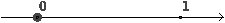
\includegraphics{figures/calculus-errors02} & ${\displaystyle f'(x_{0})=\frac{-f(x_{0})+f(x_{0}+h)}{h}-\frac{h}{2}f''(\xi_{h})}$ & Beda Maju\tabularnewline
\hline 
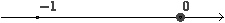
\includegraphics{figures/calculus-errors03} & ${\displaystyle f'(x_{0})=\frac{-f(x_{0}-h)+f(x_{0})}{h}+\frac{h}{2}f''(\xi_{h})}$ & Beda Mundur\tabularnewline
\hline 
\multicolumn{3}{|c|}{Rumus 3 titik}\tabularnewline
\hline 
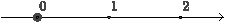
\includegraphics{figures/calculus-errors05} & ${\displaystyle f'(x_{0})=\frac{-3f(x_{0})+4f(x_{0}+h)-f(x_{0}+2h)}{2h}+\frac{h^{2}}{3}f'''(\xi_{h})}$ & Beda Maju\tabularnewline
\hline 
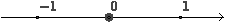
\includegraphics{figures/calculus-errors01} & ${\displaystyle f'(x_{0})=\frac{-f(x_{0}-h)+f(x_{0}+h)}{2h}+\frac{h^{2}}{6}f'''(\xi_{h})}$ & Beda Terpusat\tabularnewline
\hline 
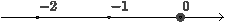
\includegraphics{figures/calculus-errors04} & ${\displaystyle f'(x_{0})=\frac{f(x_{0}-2h)-4f(x_{0}-h)+3f(x_{0})}{2h}+\frac{h^{2}}{3}f'''(\xi_{h})}$ & Beda Mundur\tabularnewline
\hline 
\multicolumn{3}{|c}{Rumus 5 titik}\tabularnewline
\hline 
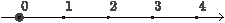
\includegraphics{figures/calculus-errors08} & ${\displaystyle f'(x_{0})=\frac{-25f(x_{0})+48f(x_{0}+h)-36f(x_{0}+2h)+16f(x_{0}+3h)-3f(x_{0}+4h)}{12h}+\frac{h^{4}}{5}f^{(5)}(\xi_{h})}$ & Beda Maju\tabularnewline
\hline 
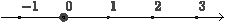
\includegraphics{figures/calculus-errors07} & ${\displaystyle f'(x_{0})=\frac{-3f(x_{0}-h)-10f(x_{0})+18f(x_{0}+h)-6f(x_{0}+2h)+f(x_{0}+3h)}{12h}+\frac{h^{4}}{20}f^{(5)}(\xi_{h})}$ & \tabularnewline
\hline 
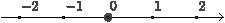
\includegraphics{figures/calculus-errors06} & ${\displaystyle f'(x_{0})=\frac{f(x_{0}-2h)-8f(x_{0}-h)+8f(x_{0}+h)-f(x_{0}+2h)}{12h}+\frac{h^{4}}{30}f^{(5)}(\xi_{h})}$ & Beda Terpusat\tabularnewline
\hline 
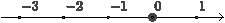
\includegraphics{figures/calculus-errors09} & ${\displaystyle f'(x_{0})=\frac{-f(x_{0}-3h)+6f(x_{0}-2h)-18f(x_{0}-h)+10f(x_{0})+3f(x_{0}+h)}{12h}+\frac{h^{4}}{20}f^{(5)}(\xi_{h})}$ & \tabularnewline
\hline 
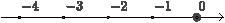
\includegraphics{figures/calculus-errors10} & ${\displaystyle f'(x_{0})=\frac{3f(x_{0}-4h)-16f(x_{0}-3h)+36f(x_{0}-2h)-48f(x_{0}-h)+25f(x_{0})}{12h}+\frac{h^{4}}{5}f^{(5)}(\xi_{h})}$ & Beda Mundur\tabularnewline
\hline 
\end{tabular}
\end{turn}
\end{table}
, \ref{tab:secondDerivativeFormulas}
\begin{table}
\caption{\label{tab:secondDerivativeFormulas}Beberapa rumus turunan kedua.}

\renewcommand{\arraystretch}{2.5}\bigskip 
\centering{}%
\begin{turn}{90}
\begin{tabular}{|c|c|c|}
\multicolumn{1}{c}{Stensil} & \multicolumn{1}{c}{Rumus} & \multicolumn{1}{c}{Nama}\tabularnewline
\hline 
\multicolumn{3}{|c|}{Rumus 3 titik}\tabularnewline
\hline 
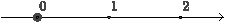
\includegraphics{figures/calculus-errors05} & ${\displaystyle f''(x_{0})=\frac{f(x_{0})-2f(x_{0}+h)+f(x_{0}+2h)}{h^{2}}+O(hf^{(3)}(\xi_{h}))}$ & Beda Maju\tabularnewline
\hline 
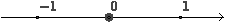
\includegraphics{figures/calculus-errors01} & ${\displaystyle f''(x_{0})=\frac{f(x_{0}-h)-2f(x_{0})+f(x_{0}+h)}{h^{2}}+O(h^{2}f^{(4)}(\xi_{h}))}$ & Beda Terpusat\tabularnewline
\hline 
\multicolumn{3}{|c|}{Rumus 4 titik}\tabularnewline
\hline 
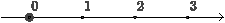
\includegraphics{figures/calculus-errors14} & ${\displaystyle f''(x_{0})=\frac{2f(x_{0})-5f(x_{0}+h)+4f(x_{0}+2h)-f(x_{0}+3h)}{h^{2}}+O(h^{2}f^{(4)}(\xi_{h}))}$ & Beda Maju\tabularnewline
\hline 
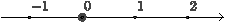
\includegraphics{figures/calculus-errors13} & ${\displaystyle f''(x_{0})=\frac{f(x_{0}-h)-2f(x_{0})+f(x_{0}+h)}{h^{2}}+O(h^{2}f^{(4)}(\xi_{h}))}$ & \tabularnewline
\hline 
\multicolumn{3}{|c}{Rumus 5 titik}\tabularnewline
\hline 
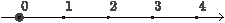
\includegraphics{figures/calculus-errors08} & ${\displaystyle f''(x_{0})=\frac{35f(x_{0})-104f(x_{0}+h)+114f(x_{0}+2h)-56f(x_{0}+3h)+11f(x_{0}+4h)}{12h^{2}}+O(h^{3}f^{(5)}(\xi_{h}))}$ & Beda Maju\tabularnewline
\hline 
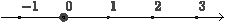
\includegraphics{figures/calculus-errors07} & ${\displaystyle f''(x_{0})=\frac{11f(x_{0}-h)-20f(x_{0})+6f(x_{0}+h)+4f(x_{0}+2h)-f(x_{0}+3h)}{12h^{2}}+O(h^{3}f^{(5)}(\xi_{h}))}$ & \tabularnewline
\hline 
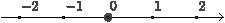
\includegraphics{figures/calculus-errors06} & ${\displaystyle f''(x_{0})=\frac{-f(x_{0}-2h)+16f(x_{0}-h)-30f(x_{0})+16f(x_{0}+h)-f(x_{0}+2h)}{12h^{2}}+O(h^{4}f^{(6)}(\xi_{h}))}$ & Beda Terpusat\tabularnewline
\hline 
\end{tabular}
\end{turn}
\end{table}
, \ref{tab:thirdDerivativeFormulas}
\begin{table}
\caption{\label{tab:thirdDerivativeFormulas}Beberapa rumus turunan ketiga.}

\renewcommand{\arraystretch}{2.5}\bigskip 
\centering{}%
\begin{turn}{90}
\begin{tabular}{|c|c|c|}
\multicolumn{1}{c}{Stensil} & \multicolumn{1}{c}{Rumus} & \multicolumn{1}{c}{Nama}\tabularnewline
\hline 
\multicolumn{3}{|c|}{Rumus 4 titik}\tabularnewline
\hline 
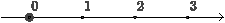
\includegraphics{figures/calculus-errors14} & ${\displaystyle f'''(x_{0})=\frac{-f(x_{0})+3f(x_{0}+h)-3f(x_{0}+2h)+f(x_{0}+3h)}{h^{3}}+O(h)f^{(4)}(\xi_{h})}$ & Beda Maju\tabularnewline
\hline 
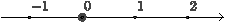
\includegraphics{figures/calculus-errors13} & ${\displaystyle f'''(x_{0})=\frac{-f(x_{0}-h)+3f(x_{0})-3f(x_{0}+h)+f(x_{0}+2h)}{h^{3}}+O(hf^{(4)}(\xi_{h}))}$ & \tabularnewline
\hline 
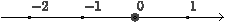
\includegraphics{figures/calculus-errors12} & ${\displaystyle f'''(x_{0})=\frac{-f(x_{0}-2h)+3f(x_{0}-h)-3f(x_{0})+f(x_{0}+h)}{h^{3}}+O(hf^{(4)}(\xi_{h}))}$ & \tabularnewline
\hline 
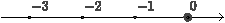
\includegraphics{figures/calculus-errors11} & ${\displaystyle f'''(x_{0})=\frac{-f(x_{0})+3f(x_{0}+h)-3f(x_{0}+2h)+f(x_{0}+3h)}{h^{3}}+O(hf^{(4)}(\xi_{h}))}$ & Beda Mundur\tabularnewline
\hline 
\multicolumn{3}{|c}{Rumus 5 titik}\tabularnewline
\hline 
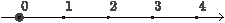
\includegraphics{figures/calculus-errors08} & ${\displaystyle f'''(x_{0})=\frac{-5f(x_{0})+18f(x_{0}+h)-24f(x_{0}+2h)+14f(x_{0}+3h)-3f(x_{0}+4h)}{2h^{3}}+O(h^{2}f^{(5)}(\xi_{h}))}$ & Beda Maju\tabularnewline
\hline 
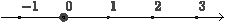
\includegraphics{figures/calculus-errors07} & ${\displaystyle f'''(x_{0})=\frac{-3f(x_{0}-h)+10f(x_{0})-12f(x_{0}+h)+6f(x_{0}+2h)-f(x_{0}+3h)}{2h^{3}}+O(h^{2}f^{(5)}(\xi_{h}))}$ & \tabularnewline
\hline 
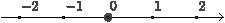
\includegraphics{figures/calculus-errors06} & ${\displaystyle f'''(x_{0})=\frac{-f(x_{0}-2h)+2f(x_{0}-h)-2f(x_{0}+h)+f(x_{0}+2h)}{2h^{3}}+O(h^{2}f^{(5)}(\xi_{h}))}$ & Beda Terpusat\tabularnewline
\hline 
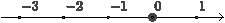
\includegraphics{figures/calculus-errors09} & ${\displaystyle f'''(x_{0})=\frac{f(x_{0}-3h)-6f(x_{0}-2h)+12f(x_{0}-h)-10f(x_{0})+3f(x_{0}+h)}{2h^{3}}+O(h^{2}f^{(5)}(\xi_{h}))}$ & \tabularnewline
\hline 
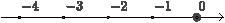
\includegraphics{figures/calculus-errors10} & ${\displaystyle f'''(x_{0})=\frac{3f(x_{0}-4h)-14f(x_{0}-3h)+24f(x_{0}-2h)-18f(x_{0}-h)+5f(x_{0})}{2h^{3}}+O(h^{2}f^{(5)}(\xi_{h}))}$ & Beda Mundur\tabularnewline
\hline 
\end{tabular}
\end{turn}
\end{table}
, dan \ref{tab:integrationFormulas}
\begin{table}
\caption{\label{tab:integrationFormulas}Beberapa rumus integrasi.}

\renewcommand{\arraystretch}{2.5}\bigskip 
\centering{}%
\begin{turn}{90}
\begin{tabular}{|c|c|c|}
\multicolumn{1}{c}{Stensil} & \multicolumn{1}{c}{Rumus} & \multicolumn{1}{c}{Nama}\tabularnewline
\hline 
\multicolumn{3}{|c|}{rumus Newton-Cotes terbuka}\tabularnewline
\hline 
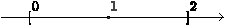
\includegraphics{figures/calculus-errors19} & ${\displaystyle \int_{x_{0}}^{x_{0}+2h}f(x)dx=2hf(x_{0}+h)+O(h^{3}f''(\xi_{h}))}$ & Aturan Titik Tengah\index{aturan titik tengah}\tabularnewline
\hline 
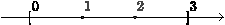
\includegraphics{figures/calculus-errors20} & ${\displaystyle \int_{x_{0}}^{x_{0}+3h}f(x)dx=\frac{3h}{2}\left[f(x_{0}+h)+f(x_{0}+2h)\right]+O(h^{3}f''(\xi_{h}))}$ & \tabularnewline
\hline 
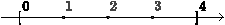
\includegraphics{figures/calculus-errors21} & ${\displaystyle \int_{x_{0}}^{x_{0}+4h}f(x)dx=\frac{4h}{3}\left[2f(x_{0}+h)-f(x_{0}+2h)+2f(x_{0}+3h)\right]+O(h^{5}f^{(4)}(\xi_{h}))}$ & \tabularnewline
\hline 
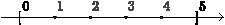
\includegraphics{figures/calculus-errors22} & ${\displaystyle \int_{x_{0}}^{x_{0}+5h}f(x)dx=\frac{5h}{24}\left[11f(x_{0}+h)+f(x_{0}+2h)+f(x_{0}+3h)+11f(x_{0}+4h)\right]+O(h^{5}f^{(4)}(\xi_{h}))}$ & \tabularnewline
\hline 
\multicolumn{3}{|c}{rumus Newton-Cotes tertutup}\tabularnewline
\hline 
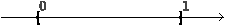
\includegraphics{figures/calculus-errors15} & ${\displaystyle \int_{x_{0}}^{x_{0}+h}f(x)dx=\frac{h}{2}\left[f(x_{0})+f(x_{0}+h)\right]+O(h^{3}f''(\xi_{h}))}$ & Aturan Trapesium\index{aturan trapesium}\tabularnewline
\hline 
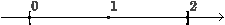
\includegraphics{figures/calculus-errors16} & ${\displaystyle \int_{x_{0}}^{x_{0}+2h}f(x)dx=\frac{h}{3}\left[f(x_{0})+4f(x_{0}+h)+f(x_{0}+2h)\right]+O(h^{5}f^{(4)}(\xi_{h}))}$ & Aturan Simpson\index{aturan Simpson}\tabularnewline
\hline 
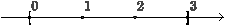
\includegraphics{figures/calculus-errors17} & ${\displaystyle \int_{x_{0}}^{x_{0}+3h}f(x)dx=\frac{3h}{8}\left[f(x_{0})+3f(x_{0}+h)+3f(x_{0}+2h)+f(x_{0}+3h)\right]+O(h^{5}f^{(4)}(\xi_{h}))}$ & Aturan Simpson $\frac{3}{8}$\index{aturan Simpson@aturan Simpson $\frac{3}{8}$}\tabularnewline
\hline 
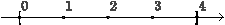
\includegraphics{figures/calculus-errors18} & ${\displaystyle \int_{x_{0}}^{x_{0}+4h}f(x)dx=\frac{2h}{45}\left[7f(x_{0})+32f(x_{0}+h)+12f(x_{0}+2h)+32f(x_{0}+3h)+7f(x_{0}+4h)\right]+O(h^{7}f^{(6)}(\xi_{h}))}$ & Aturan Bode\index{aturan Bode}\tabularnewline
\hline 
\multicolumn{3}{|c}{rumus kuadratur Gauss}\tabularnewline
\hline 
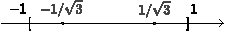
\includegraphics{figures/calculus-errors23} & ${\displaystyle \int_{x_{0}-h}^{x_{0}+h}f(x)dx=h\left[f\left(x_{0}-\frac{1}{\sqrt{3}}h\right)+f\left(x_{0}+\frac{1}{\sqrt{3}}h\right)\right]+O(h^{5}f^{(4)}(\xi_{h}))}$ & \tabularnewline
\hline 
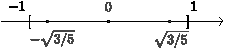
\includegraphics{figures/calculus-errors24} & ${\displaystyle \int_{x_{0}-h}^{x_{0}+h}f(x)dx=\frac{h}{9}\left[5f\left(x_{0}-\sqrt{\frac{3}{5}}h\right)+8f(x_{0})+5f\left(x_{0}+\sqrt{\frac{3}{5}}h\right)\right]+O(h^{7}f^{(6)}(\xi_{h}))}$ & \tabularnewline
\hline 
\end{tabular}
\end{turn}
\end{table}
 merangkum beberapa rumus standar untuk turunan dan integral. Perhatikan
bahwa tidak ada rumus satu titik untuk turunan apa pun, tidak ada
rumus dua titik untuk turunan kedua atau yang lebih tinggi, dan tidak
ada rumus tiga titik untuk turunan ketiga atau yang lebih tinggi.
Stensil telah disederhanakan agar hanya menampilkan nilai $\theta_{i}$.
Dengan demikian, stensil 
\begin{center}
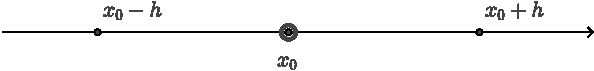
\includegraphics{figures/calculus-rudiments03}
\par\end{center}

\noindent ditampilkan dalam tabel sebagai

\begin{center}
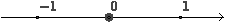
\includegraphics[scale=2]{figures/calculus-errors01}.
\par\end{center}

\subsection{Konsep Kunci}
\begin{description}
\item [{Derajat~ketelitian:~\index{ketelitian!derajat}Bilangan}] bulat
$m$ sedemikian rupa sehingga suatu rumus kalkulus numerik eksak untuk
semua polinom hingga dan termasuk derajat $m$ tetapi tidak eksak
untuk semua polinom berderajat $m+1$.
\item [{Suku~galat:}] Suku galat untuk hampiran kalkulus numerik dapat
ditemukan dengan mengganti setiap kemunculan $f$ dalam rumus hampiran
dengan ekspansi deret Taylor di sekitar $x_{0}$ lalu menyederhanakannya.
\item [{Kuadratur~Gauss:}] \index{kuadratur!Gauss}Metode kuadratur yang
memaksimalkan derajat ketelitian relatif terhadap jumlah simpul yang
digunakan.
\item [{Kuadratur:}] \index{kuadratur}\index{kuadratur|seealso{integrasi numerik}}Nama
lain untuk rumus integrasi numerik.
\item [{Laju~kekonvergenan:~\index{O besar}\index{kekonvergenan!laju}Untuk}] fungsi
$g(h)$ yang memenuhi ${\displaystyle \lim_{h\to0}g(h)=0}$, $p(h)=O(g(h))$
berarti bahwa $|p(h)|\leq M|g(h)|$ untuk suatu konstanta $M$ dan
$h$ yang cukup kecil.
\item [{Teorema~Nilai~Rata-Rata~Berbobot:}] \index{Teorema!Nilai Rata-Rata Berbobot}Asumsikan
bahwa $f$ dan $g$ kontinu pada $[a,b]$. Jika $g$ tidak pernah
berubah tanda dan bernilai nonnegatif pada $[a,b]$, maka berlaku
\[
\int_{a}^{b}f(x)g(x)dx=f(c)\int_{a}^{b}g(x)dx
\]
untuk suatu $c$ di $(a,b)$. 
\end{description}
\begin{small} 

\newpage{}

\subsection{Latihan}
\begin{enumerate}
\item Misalkan $f(x)=e^{x}-\sin x$. Lengkapilah tabel berikut menggunakan
rumus hampiran
\[
f'(x_{0})\approx\frac{-3f(x_{0})+4f(x_{0}+h)-f(x_{0}+2h)}{2h}.
\]

\begin{center}
\begin{tabular}{c|c|c}
$h$ & hampiran $f'(2)$ & galat absolut\tabularnewline
\hline 
$.01$ &  & \tabularnewline
$.005$ &  & \tabularnewline
$-.005$ &  & \tabularnewline
$-.01$ &  & \tabularnewline
\end{tabular}
\par\end{center}

Bolehkah menggunakan nilai negatif untuk $h$?
\item \label{exc:calculusErrors-4} Untuk setiap nilai $x$ dalam tabel,
gunakan rumus tiga titik paling akurat untuk menghampiri $f'(x)$. \hasananswer 

\begin{center}
\begin{tabular}{c|c|c}
$x$ & $f(x)$ & $f'(x)$\tabularnewline
\hline 
$-2.7$ & $0.054797$ & \tabularnewline
$-2.5$ & $0.11342$ & \tabularnewline
$-2.3$ & $0.65536$ & \tabularnewline
$-2.1$ & $0.98472$ & \tabularnewline
\end{tabular}
\par\end{center}
\item \label{exc:calculusErrors}Hampiri integral tersebut menggunakan aturan
Simpson.

\begin{enumerate}
\item \label{exc:calculusErrors-5}${\displaystyle \int_{-0.5}^{0}x\ln(x+1)dx}$ \hasasolution 
\item $\int_{1}^{3}\ln(x+1)\,dx$
\item \label{exc:calculusErrors-6}${\displaystyle \int_{-0.25}^{0.25}(\cos x)^{2}dx}$ \hasananswer 
\item \label{exc:calculusErrors-41}$\int_{1}^{3}e^{\sin x}\:dx$
\item \label{exc:calculusErrors-7}$\int_{1}^{2}x^{4}\,dx$ \hasananswer 
\end{enumerate}
\item \label{exc:calculusErrors-1}Kerjakan soal \ref{exc:calculusErrors}
dengan menggunakan aturan Trapesium. \haspartwithsolution \haspartwithanswer 
\item \label{exc:calculusErrors-2}Kerjakan soal \ref{exc:calculusErrors}
dengan menggunakan Aturan Titik Tengah. \haspartwithsolution \haspartwithanswer 
\item \label{exc:calculusErrors-37}Tentukan galat hampiran pada soal \ref{exc:calculusErrors}.
Anda dapat menggunakan $4.4247999271351$ sebagai nilai eksak integral
pada \ref{exc:calculusErrors-41}. \haspartwithsolution \haspartwithanswer 
\item \label{exc:calculusErrors-38}Tentukan galat hampiran pada soal \ref{exc:calculusErrors-1}.
Anda dapat menggunakan $4.4247999271351$ sebagai nilai eksak integral
pada \ref{exc:calculusErrors-41}. \haspartwithsolution \haspartwithanswer 
\item \label{exc:calculusErrors-39}Tentukan galat hampiran pada soal \ref{exc:calculusErrors-2}.
Anda dapat menggunakan $4.4247999271351$ sebagai nilai eksak integral
pada \ref{exc:calculusErrors-41}. \haspartwithsolution \haspartwithanswer 
\item Tentukan galat dalam menghampiri $\int_{-7}^{11}(32x^{2}+\sqrt{7}x-2)dx$
menggunakan Aturan Simpson $\frac{3}{8}$.
\item \label{exc:calculusErrors-19}Tentukan galat dalam menghampiri $\int_{-17}^{36}(32x^{5}+7x^{3}-2)dx$
menggunakan Aturan Bode. \hasananswer 
\item \label{exc:calculusErrors-3}Untuk nilai $f$, $x_{0}$, dan $h$
berikut, gunakan rumus 
\[
f'(x_{0})=\frac{f(x_{0}+h)-f(x_{0}-h)}{2h}-\frac{h^{2}}{6}f'''(\xi)
\]
untuk menghampiri $f'(x_{0})$.

\begin{enumerate}
\item \label{exc:calculusErrors-36}$f(x)=e^{x}$; $x_{0}=2$; $h=0.1$. \hasasolution 
\item \label{exc:calculusErrors-20}$f(x)=(\cosh2x)^{2}-\sin x$; $x_{0}=\pi$;
$h=0.05$. \hasananswer 
\item $f(x)=\ln(2x-3)+5x$; $x=10$; $h=1$.
\end{enumerate}
\item \label{exc:calculusErrors-8}Hitung batas bawah dan batas atas bagi
galat hampiran pada soal \ref{exc:calculusErrors-3}. Pastikan bahwa
galat sebenarnya berada di antara kedua batas tersebut. \haspartwithsolution  \haspartwithanswer 
\item \label{exc:calculusErrors-9}Untuk setiap bagian soal \ref{exc:calculusErrors-3},
tentukan nilai $\xi$ yang dijamin oleh rumus tersebut. \haspartwithsolution  \haspartwithanswer 
\item Nyatakan derajat ketelitian rumus Newton-Cotes tertutup dengan 5 simpul,
yaitu Aturan Bode.
\item \label{exc:calculusErrors-10}Nyatakan derajat ketelitian rumus lima
titik berikut. \hasasolution 
\begin{align*}
f'(x_{0})=\frac{1}{12h}\left[-25f(x_{0})+48f(x_{0}+h)-36f(x_{0}+2h)\right.\qquad\\
\left.+16f(x_{0}+3h)-3f(x_{0}+4h)\right]+\frac{h^{4}}{5}f^{(5)}(\xi)
\end{align*}
\item Tentukan derajat ketelitian rumus kuadratur
\[
\int_{3}^{5}f(x)\,dx\approx\frac{1}{2}\left[3f\left(\frac{11}{3}\right)+f(5)\right].
\]
\item Tentukan suku galat metode kuadratur tersebut dan nyatakan derajat
ketelitiannya.

\begin{enumerate}
\item \label{exc:calculusErrors-21}${\displaystyle \int_{x_{0}}^{x_{0}+h}f(x)\,dx\approx hf(x_{0})}$ \hasananswer 
\item ${\displaystyle \int_{x_{0}}^{x_{0}+h}f(x)\,dx\approx hf\left(x_{0}+\frac{h}{4}\right)}$
\item \label{exc:calculusErrors-11}${\displaystyle \int_{x_{0}}^{x_{0}+h}f(x)dx\approx\frac{h}{4}\left[3f\left(x_{0}+\frac{2}{3}h\right)+f(x_{0})\right]}$ \hasasolution 
\item ${\displaystyle \int_{x_{0}}^{x_{0}+2h}f(x)dx\approx\frac{h}{2}\left[3f\left(x_{0}+\frac{4}{3}h\right)+f(x_{0})\right]}$
\item \label{exc:calculusErrors-22}${\displaystyle \int_{x_{0}}^{x_{0}+3h}f(x)dx\approx\frac{3h}{4}\left[f(x_{0})+3f(x_{0}+2h)\right]}$ \hasananswer 
\item ${\displaystyle \int_{x_{0}}^{x_{0}+2h}f(x)dx\approx\frac{h}{2}\left[f\left(x_{0}-\frac{h}{2}\right)+3f\left(x_{0}+\frac{3}{2}h\right)\right]}$
\item \label{exc:calculusErrors-23}${\displaystyle \int_{x_{0}}^{x_{0}+2h}f(x)dx\approx\frac{h}{3}\left[f(x_{0}-h)-2f(x_{0})+7f(x_{0}+h)\right]}$ \hasananswer 
\item ${\displaystyle \int_{x_{0}}^{x_{0}+3h}f(x)dx\approx3h\left[3f\left(x_{0}+\frac{3}{2}h\right)-6f(x_{0}+h)+4f\left(x_{0}+\frac{3}{4}h\right)\right]}$
\item \label{exc:calculusErrors-24}${\displaystyle \int_{x_{0}}^{x_{0}+3h}f(x)dx\approx-\frac{h}{12}\left[208f\left(x_{0}+\frac{3}{2}h\right)-891f(x_{0}+h)+1344f\left(x_{0}+\frac{3}{4}h\right)-625f\left(x_{0}+\frac{3}{5}h\right)\right]}$ \hasananswer 
\end{enumerate}
\item Tentukan suku galat hampiran turunan berikut:

\begin{enumerate}
\item \label{exc:calculusErrors-25}${\displaystyle f'(x_{0})\approx\frac{f(x_{0}+2h)-f(x_{0})}{2h}}$ \hasananswer 
\item ${\displaystyle f'(x_{0})\approx\frac{f(x_{0}+2h)-f(x_{0}-h)}{3h}}$
\item \label{exc:calculusErrors-12}${\displaystyle f'(x_{0})\approx\frac{-3f(x_{0})+4f(x_{0}+\frac{h}{2})-f(x_{0}+h)}{h}}$ \hasasolution 
\item ${\displaystyle f'(x_{0})\approx\frac{-13f(x_{0}-10h)-12f(x_{0}+5h)+25f(x_{0}+8h)}{270h}}$
\item \label{exc:calculusErrors-26}${\displaystyle f'(x_{0})\approx\frac{-7f(x_{0}+h)+416f(x_{0}+\frac{1}{2}h)-2916f(x_{0}+\frac{1}{3}h)+5632f(x_{0}+\frac{1}{4}h)-3125f(x_{0}+\frac{1}{5}h)}{12h}}$ \hasananswer 
\item ${\displaystyle f''(x_{0})\approx\frac{2f(x_{0}-h)-3f(x_{0})+f(x_{0}+2h)}{3h^{2}}}$
\item \label{exc:calculusErrors-27}${\displaystyle f''(x_{0})\approx\frac{7f(x_{0}-5h)-12f(x_{0})+5f(x_{0}+7h)}{210h^{2}}}$ \hasananswer 
\item ${\displaystyle f''(x_{0})\approx\frac{5f(x_{0}-5h)-12f(x_{0}+2h)+7f(x_{0}+7h)}{210h^{2}}}$
\item \label{exc:calculusErrors-28}${\displaystyle f''(x_{0})\approx\frac{5f(x_{0}-2h)+32f(x_{0}-h)-60f(x_{0})+25f(x_{0}+2h)-2f(x_{0}+4h)}{60h^{2}}}$ \hasananswer 
\end{enumerate}
\item \label{exc:calculusErrors-17}Diffy Rence menuliskan hampiran berikut:
\[
f''(3.0)\approx25[\sin(2.8)-2\sin(3.0)+\sin(3.2)].
\]

Apa bentuk fungsi $f(x)$? \hasasolution 
\item Misalkan $f(x)=\sin x$. 

\begin{enumerate}
\item Tentukan batas galat untuk hampiran 
\[
f'(6)\approx\frac{-3\sin6+4\sin6.1-\sin6.2}{0.2}
\]
 berdasarkan suku galat yang sesuai.
\item Bandingkan batas ini dengan galat sebenarnya.
\end{enumerate}
\item Apa yang dapat Anda simpulkan tentang galat dalam menghampiri turunan
pertama fungsi 
\[
f(x)=-13x^{4}+17x^{3}-15x^{2}+12x-99
\]
dengan rumus lima titik?
\item Misalkan $f(x)=3x^{3}-2x^{2}+x$.

\begin{enumerate}
\item Hitung galat (bukan batas galat) ketika menaksir $f'(2)$ menggunakan
beda maju
\[
\frac{f(x_{0}+h)-f(x_{0})}{h}
\]
dengan $h=0.1$.
\item Tentukan $\xi_{0.1}$ yang keberadaannya dijamin oleh suku galat.
\end{enumerate}
\item Misalkan $f(x)=\sin x$.  Tentukan batas galat hampiran tersebut.

\begin{enumerate}
\item \label{exc:calculusErrors-29}${\displaystyle f''(3.0)\approx25[\sin(2.8)-2\sin(3.0)+\sin(3.2)]}$ \hasananswer 
\item ${\displaystyle f''(3.0)\approx1600\left[2\sin(3.0)-5\sin(3.025)+4\sin(3.05)-\sin(3.075)\right]}$
\item \label{exc:calculusErrors-13}$f'''(3.0)\approx500000\left[-5\sin(3.0)+18\sin(3.01)-24\sin(3.02)+14\sin(3.03)-3\sin(3.04)\right]$ \hasasolution 
\item ${\displaystyle f'''(3.0)\approx1000\left[-\sin(2.8)+3\sin(2.9)-3\sin(3.0)+\sin(3.1)\right]}$
\item ${\displaystyle \int_{3}^{4}f(x)dx\approx\frac{1}{6}\left[\sin(3)+4\sin(3.5)+\sin(4)\right]}$
\item \label{exc:calculusErrors-14}${\displaystyle \int_{3}^{4}f(x)dx\approx\frac{1}{2}\left[\sin\left(\frac{7}{2}-\frac{1}{2\sqrt{3}}\right)+\sin\left(\frac{7}{2}+\frac{1}{2\sqrt{3}}\right)\right]}$ \hasasolution 
\end{enumerate}
\item \label{exc:calculusErrors-18}Misalkan Anda memiliki data berikut
untuk suatu fungsi $f$. \hasasolution 

\begin{center}
\begin{tabular}{cccccc}
$x$ & $0$ & $1$ & $2$ & $3$ & $4$\tabularnewline
$f(x)$ & $-0.2381$ & $-0.3125$ & $-0.4545$ & $-0.8333$ & $-5$\tabularnewline
\end{tabular}
\par\end{center}
\begin{enumerate}
\item Hampiri $f'(4)$ dan $f'(2)$ menggunakan rumus lima titik. 
\item Menurut Anda, hampiran manakah yang akan lebih akurat, dan mengapa?
\item Apakah hasilnya memang demikian? Data tersebut berasal dari $f(x)=\frac{1}{x-4.2}$.
\end{enumerate}
\item \label{exc:calculusErrors-30}Gunakan metode kuadratur 
\[
\int_{x_{0}}^{x_{0}+h}f(x)\,dx=\frac{h}{2}\left[f\left(x_{0}+\frac{h}{3}\right)+f\left(x_{0}+\frac{2h}{3}\right)\right]+\frac{h^{3}}{36}f''(\xi)
\]
untuk semua pertanyaan berikut. \hasananswer 

\begin{enumerate}
\item Berapakah laju kekonvergenannya?
\item Berapakah derajat ketelitiannya?
\item Gunakan metode tersebut untuk menghampiri $\int_{0}^{\pi}\sin x\,dx$.
\item Tentukan batas galat hampiran ini.
\item Bandingkan batas tersebut dengan galat sebenarnya.
\end{enumerate}
\item Penerapan Aturan Trapesium pada ${\displaystyle \int_{0}^{2}f(x)dx}$
menghasilkan nilai 5, sedangkan Aturan Titik Tengah menghasilkan nilai
4. Nilai berapakah yang diberikan oleh Aturan Simpson?
\item \label{exc:calculusErrors-31}Penerapan Aturan Trapesium pada $\int_{0}^{2}f(x)\,dx$
menghasilkan nilai 4, sedangkan Aturan Simpson menghasilkan nilai
2. Berapakah $f(1)$? \hasananswer 
\item \label{exc:calculusErrors-32}Jika $f'''(x_{0})$ dihampiri menggunakan
lima simpul, berapakah laju kekonvergenan minimalnya?  \hasananswer 
\item Tunjukkan bahwa rata-rata dari hampiran beda maju $\frac{-f(x_{0})+f(x_{0}+h)}{h}$
dan hampiran beda mundur $\frac{-f(x_{0}-h)+f(x_{0})}{h}$ untuk $f'(x_{0})$
menghasilkan hampiran beda terpusat $\frac{f(x_{0}+h)-f(x_{0}-h)}{2h}$
untuk $f'(x_{0})$.
\item \label{exc:calculusErrors-33}Chuck sedang ``menghampiri'' suatu
integral tentu menggunakan Aturan Simpson. Seperti tampak dari pengerjaannya
di bawah ini, ia sedang mengintegralkan polinom kubik. Hitung galat
yang ditimbulkannya meskipun Anda tidak dapat membaca semua koefisiennya. \hasananswer 

\begin{center}
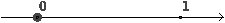
\includegraphics[width=2.5in]{figures/calculus-errors02}
\par\end{center}
\item \label{exc:calculusErrors-40}Ulangi \ref{exc:calculusErrors-33},
kali ini dengan asumsi Chuck menggunakan Aturan Trapesium. \hasananswer 
\item Sketsakan grafik suatu fungsi $f(x)$, lalu tandai nilai $x_{0}$
dan $h$ pada grafik tersebut sedemikian sehingga beda mundur $\frac{f(x_{0})-f(x_{0}-h)}{h}$
menghasilkan hampiran yang \textbf{\emph{lebih baik}} untuk $f'(x_{0})$
daripada beda terpusat $\frac{f(x_{0}+h)-f(x_{0}-h)}{2h}$.
\item \label{exc:calculusErrors-15}Sketsakan grafik suatu fungsi $f(x)$
sedemikian sehingga Aturan Trapesium memberikan hampiran yang lebih
baik untuk $\int_{0}^{1}f(x)\,dx$ daripada Aturan Simpson, lalu jelaskan
bagaimana Anda mengetahuinya. \hasasolution 
\item \label{exc:calculusErrors-16}Misalkan rumus lima titik digunakan
untuk menghampiri $f''(x_{0})$ dengan ukuran langkah $h=0.1$ dan
$h=0.02$. Jika $E_{0.1}$ menyatakan galat hampiran untuk $h=0.1$
dan $E_{0.02}$ menyatakan galat hampiran untuk $h=0.02$, kira-kira
berapakah nilai $\frac{E_{0.1}}{E_{0.02}}$ yang Anda harapkan? \hasasolution 
\item Rumus umum tiga titik yang menggunakan simpul $x_{0}$, $x_{0}+\alpha h$,
dan $x_{0}+2h$, dengan $(\alpha\neq0,2)$, diberikan oleh
\[
f'(x_{0})\approx\frac{1}{2h}\left[-\frac{2+\alpha}{\alpha}f(x_{0})+\frac{4}{\alpha(2-\alpha)}f(x_{0}+\alpha h)-\frac{\alpha}{2-\alpha}f(x_{0}+2h)\right].
\]

\begin{enumerate}
\item Tunjukkan bahwa rumus ini menyederhana menjadi salah satu rumus standar
untuk $\alpha=1$.
\item Tentukan suku galat rumus ini.
\end{enumerate}
\item \label{exc:calculusErrors-34}Tentukan tiga hampiran berbeda untuk
$f'(0.2)$ dengan menggunakan rumus tiga titik. \hasananswer 

\begin{center}
\begin{tabular}{c|c}
$x$ & $f(x)$\tabularnewline
\hline 
$0$ & $1$\tabularnewline
$0.1$ & $1.10517$\tabularnewline
$0.2$ & $1.22140$\tabularnewline
$0.3$ & $1.34986$\tabularnewline
$0.4$ & $1.49182$\tabularnewline
\end{tabular}
\par\end{center}

Grafik $f'''(x)$ ditampilkan di bawah ini. Gunakan grafik tersebut
untuk mengurutkan ketiga hampiran Anda dari yang diperkirakan memiliki
galat terkecil hingga terbesar, lalu jelaskan alasan urutan tersebut.

\begin{center}
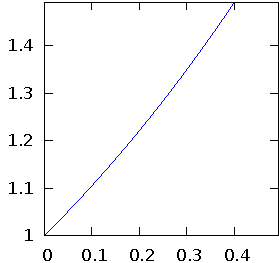
\includegraphics{figures/calculus-errors25}
\par\end{center}
\item Verifikasikan secara numerik bahwa galat saat rumus $f'(x_{0})=\frac{-2f(x_{0}-h)-3f(x_{0})+6f(x_{0}+h)-f(x_{0}+2h)}{6h}$
digunakan untuk menghampiri $f'(3)$ dengan fungsi $f(x)=(\cos3x)^{2}+\ln x$
memang berorde $O(h^{3})$.
\item \label{exc:calculusErrors-35}Dengan komputasi presisi ganda (Octave
standar), tentukan secara numerik taksiran terbaik yang dapat diperoleh
dari rumus 
\[
f'(3)=\frac{-2f(3-h)-3f(3)+6f(3+h)-f(3+2h)}{6h}
\]
 untuk $f(x)=(\cos3x)^{2}+\ln x$. Nilai $h$ berapakah yang menghasilkan
hampiran optimal tersebut? \hasananswer 
\item Tentukan derajat ketelitian rumus kuadratur berikut:
\[
\int_{-1}^{1}f(x)dx=f\left(-\frac{\sqrt{3}}{3}\right)+f\left(\frac{\sqrt{3}}{3}\right).
\]
\item Rumus kuadratur ${\displaystyle \int_{0}^{2}f(x)dx=c_{0}f(0)+c_{1}f(1)+c_{2}f(2)}$
eksak untuk semua polinom berderajat kurang dari atau sama dengan
2. Tentukan $c_{0}$, $c_{1}$, dan $c_{2}$.
\end{enumerate}
\end{small}



\section{\label{sec:Composite}Integrasi Komposit\index{integrasi numerik!komposit}}

Pada bagian \ref{sec:calculusErrorAnalysis} kita memberikan suku-suku
galat yang berbentuk $O(h^{k}f^{(l)}(\xi_{h}))$. Sebagai contoh utama,
Aturan Trapesium, ${\displaystyle \int_{x_{0}}^{x_{0}+h}f(x)dx=\frac{h}{2}\left[f(x_{0})+f(x_{0}+h)\right]+O(h^{3}f''(\xi_{h}))}$,
memiliki suku galat $O(h^{3}f''(\xi_{h}))$. Kesimpulan ini diperoleh
langsung dari analisis deret Taylor, tetapi apa artinya?

Suku galat untuk hampiran turunan relatif mudah dipahami. Pertimbangkan
hampiran turunan pertama ${\displaystyle f'(x_{0})=\frac{-f(x_{0}-h)+f(x_{0}+h)}{2h}+\frac{h^{2}}{6}f'''(\xi_{h})}$.
Semakin kecil $h$, semakin kecil pula galat dalam menghampiri $f'(x_{0})$
(selama suku $f'''(\xi_{h})$ tidak meniadakan manfaat dari mengecilkan
$h$). Suku galat untuk hampiran integral tidak semudah itu dipahami
karena, dalam setiap kasus, besaran yang dihampiri bergantung pada
$h$. Mengubah $h$ dalam rumus integrasi juga mengubah besaran yang
dihampiri. Hal ini berlaku untuk setiap rumus dalam tabel \ref{tab:integrationFormulas}.
Aturan Trapesium merupakan contoh yang baik untuk tujuan ini. Ruas
kiri, yaitu besaran yang dihampiri, adalah $\int_{x_{0}}^{x_{0}+h}f(x)dx$,
sehingga $h$ yang lebih kecil berarti menghampiri integral pada selang
yang lebih kecil. Jadi, bagaimana galat yang lebih kecil saat menghampiri
bilangan lain dapat memberi tahu kita tentang manfaat potensial menghitung
dengan nilai $h$ yang lebih kecil? Telaah cermat terhadap Aturan
Trapesium akan mengungkap jawabannya.

Menurut Aturan Trapesium, $\frac{h}{2}\left[f(x_{0})+f(x_{0}+h)\right]$
menghampiri integral $f$ pada selang $[x_{0},x_{0}+h]$. Jika $h$
diganti dengan $h/2$, hampiran yang dihasilkan, $\frac{h}{4}\left[f(x_{0})+f(x_{0}+\frac{h}{2})\right]$,
merupakan hampiran bagi integral $f$ pada selang $[x_{0},x_{0}+\frac{h}{2}]$.
Besaran itu bukan lagi hampiran bagi integral pada $[x_{0},x_{0}+h]$!
Untuk menggunakan Aturan Trapesium guna menghampiri besaran semula,
yakni integral $f$ pada $[x_{0},x_{0}+h]$, penggunaan $h/2$ sebagai
pengganti $h$ memerlukan dua penerapan Aturan Trapesium---satu pada
selang $[x_{0},x_{0}+\frac{h}{2}]$ dan satu lagi pada selang $[x_{0}+\frac{h}{2},x_{0}+h]$.
Jumlah kedua hampiran ini merupakan hampiran bagi integral $f$ pada
$[x_{0},x_{0}+h]$. Jika $h$ diperkecil lagi, Aturan Trapesium harus
diterapkan pada lebih banyak selang. Secara umum, memperkecil $h$
menjadi $\frac{h}{n}$ untuk sembarang bilangan bulat $n$ memerlukan
$n$ penerapan Aturan Trapesium:
\begin{eqnarray}
\int_{x_{0}}^{x_{0}+h}f(x)dx & = & \int_{x_{0}}^{x_{0}+\frac{h}{n}}f(x)dx+\int_{x_{0}+\frac{h}{n}}^{x_{0}+2\frac{h}{n}}f(x)dx+\cdots+\int_{x_{0}+(n-1)\frac{h}{n}}^{x_{0}+h}f(x)dx\nonumber \\
 & \approx & \frac{h}{2n}\left[f(x_{0})+f\left(x_{0}+\frac{h}{n}\right)\right]+\frac{h}{2n}\left[f\left(x_{0}+\frac{h}{n}\right)+f\left(x_{0}+2\frac{h}{n}\right)\right]+\nonumber \\
 &  & \qquad\qquad\qquad\cdots+\frac{h}{2n}\left[f\left(x_{0}+(n-1)\frac{h}{n}\right)+f(x_{0}+h)\right].\label{eq:compositeTrapezoidal}
\end{eqnarray}
Menguraikan $\int_{x_{0}}^{x_{0}+h}f(x)dx$ menjadi jumlah $\int_{x_{0}}^{x_{1}}f(x)dx+\int_{x_{1}}^{x_{2}}f(x)dx+\cdots+\int_{x_{n-1}}^{x_{n}}f(x)dx$
lalu menjumlahkan hampiran integral-integral tersebut disebut integrasi
komposit.

Untuk penggunaan Aturan Trapesium dalam penghampiran, galat pada satu
kali penerapan Aturan Trapesium adalah $O(h^{3}f''(\xi_{h}))$. Karena
itu, galat dalam jumlah di atas dibatasi oleh $\sum_{i=1}^{n}M\left(\frac{h}{n}\right)^{3}f''(\mu_{i})=Mh\left(\frac{h}{n}\right)^{2}\cdot\frac{1}{n}\sum_{i=1}^{n}f''(\mu_{i})$
untuk suatu $\mu_{i}$ dengan $x_{0}+(i-1)\frac{h}{n}<\mu_{i}<x_{0}+i\frac{h}{n}$.
Dengan mengasumsikan $f''$ kontinu pada $[x_{0},x_{0}+h]$, teorema
nilai antara memungkinkan kita mengganti $\frac{1}{n}\sum_{i=1}^{n}f''(\mu_{i})$
dengan $f''(\xi_{n})$ untuk suatu $\xi_{n}\in(x_{0},x_{0}+h)$ karena
$\frac{1}{n}\sum_{i=1}^{n}f''(\mu_{i})$ merupakan rata-rata dari
$f''(\mu_{i})$, yang tidak melebihi nilai maksimum $f''(\mu_{i})$
dan tidak kurang dari nilai minimum $f''(\mu_{i})$. Penggantian ini
memberi kita batas galat $Mh\left(\frac{h}{n}\right)^{2}f''(\xi_{n})$.
Kesimpulannya, Aturan Trapesium yang digunakan berulang kali bila
diperlukan untuk menghampiri $\int_{x_{0}}^{x_{0}+h}f(x)dx$ sebenarnya
memiliki galat $O\left(\left(\frac{1}{n}\right)^{2}f''(\xi_{n})\right)$,
dengan $n$ adalah banyaknya subselang yang digunakan dalam perhitungan
dan $\xi_{n}$ bergantung pada $n$. Kini sifat galat tersebut lebih
jelas. Galat itu ditentukan oleh banyaknya subselang yang digunakan
dalam perhitungan. Lebih banyak subselang ($n$ yang lebih besar)
berarti galat lebih kecil (dengan asumsi manfaat penambahan subselang
tidak ditiadakan oleh faktor $f''$). Rumus integrasi komposit lainnya
serupa. Jika rumus kuadratur satu selang memiliki galat $O(h^{k}f^{(l)}(\xi_{h}))$,
versi komposit yang bersesuaian memiliki galat $O\left(\left(\frac{1}{n}\right)^{k-1}f^{(l)}(\xi_{n})\right)$.
Secara umum, lebih banyak selang berarti galat lebih kecil. 

\begin{digression}{galat anomali}

\noindent Dari tabel pada akhir bagian \ref{sec:calculusErrorAnalysis},
Anda dapat melihat bahwa galat Aturan Simpson adalah $O(h^{5}f^{(4)}(\xi_{h}))$,
sehingga kita memperkirakan galat Aturan Simpson komposit sebesar
$O\left(\frac{1}{n^{4}}f^{(4)}(\xi_{n})\right)$. Berdasarkan definisi,
notasi O besar digunakan untuk menyatakan batas atas galat; jadi,
sesungguhnya kita memperkirakan bahwa galat Aturan Simpson komposit
\textbf{tidak lebih dari } $O\left(\frac{1}{n^{4}}f^{(4)}(\xi_{n})\right)$.
Bahkan, dalam beberapa kasus kita memperoleh kekonvergenan yang lebih
baik daripada perkiraan! Salah satu contoh menarik fenomena ini adalah
penerapan Aturan Simpson komposit pada integral ${\displaystyle \int_{0}^{1}\frac{1}{1+x^{2}}dx}$,
yang nilai eksaknya adalah $\frac{\pi}{4}$. Tabel di bawah menunjukkan
bahwa rasio galat mendekati $2^{6}$, bukan $2^{4}$ ketika banyaknya
subselang digandakan. Terdapat sesuatu yang sangat khusus pada kombinasi
fungsi dan selang ini. Cobalah mengulangi eksperimen ini dengan fungsi
yang sama pada selang berbeda atau dengan fungsi berbeda pada selang
yang sama.
\begin{center}
\begin{tabular}{c|ccc}
subselang, $i$ & Aturan Simpson komposit & galat mutlak, $e_{i}$ & rasio galat, $\frac{e_{i}}{e_{i+1}}$\tabularnewline
\hline 
$4$ & $0.785398125614677$ & $3.77827(10)^{-8}$ & $63.90$\tabularnewline
$8$ & $0.785398162806206$ & $5.91242(10)^{-10}$ & $63.99$\tabularnewline
$16$ & $0.785398163388209$ & $9.23916(10)^{-12}$ & $64.06$\tabularnewline
$32$ & $0.785398163397304$ & $1.44217(10)^{-13}$ & \tabularnewline
\end{tabular}
\par\end{center}

\noindent Terima kasih kepada John George atas contoh ini!

\end{digression}

\subsection{Aturan Trapesium Komposit\index{aturan trapesium!komposit}}

Persamaan \ref{eq:compositeTrapezoidal} merangkum Aturan Trapesium
komposit, tetapi bukan merupakan cara paling efisien untuk menggunakannya.
Penyederhanaan ungkapan tersebut akan membantu. Perhatikan bahwa semua
penghitungan nilai fungsi selain $f(x_{0})$ dan $f(x_{0}+h)$ muncul
dua kali, sehingga rumusnya dapat dipadatkan menjadi
\begin{eqnarray*}
\int_{x_{0}}^{x_{0}+h}f(x)dx & \approx & \frac{h}{2n}\left[f(x_{0})+f(x_{0}+h)\right]+\frac{h}{n}\left[f\left(x_{0}+\frac{h}{n}\right)+\cdots+f\left(x_{0}+(n-1)\frac{h}{n}\right)\right]\\
 & = & \frac{h}{2n}\left[f(x_{0})+f(x_{0}+h)+2\sum_{i=1}^{n-1}f\left(x_{0}+i\frac{h}{n}\right)\right]\\
 & = & \frac{h}{n}\left[\frac{f(x_{0})+f(x_{0}+h)}{2}+\sum_{i=1}^{n-1}f\left(x_{0}+i\frac{h}{n}\right)\right].
\end{eqnarray*}
Ini menghasilkan kode semu berikut setelah kita melakukan substitusi
$a=x_{0}$ dan $b=x_{0}+h$.

\noindent\begin{pseudocode} \index{aturan trapesium!komposit, kode semu}
\begin{description}
\item [{Asumsi:}] $f$ memiliki turunan kedua yang kontinu pada $[a,b]$.
\item [{Masukan:}] Fungsi $f$; selang integrasi $[a,b]$; banyaknya subselang
$n$.
\item [{Langkah~1:}] Tetapkan $h=b-a$; $d=\frac{h}{n}$; $I=\frac{f(a)+f(b)}{2}$;
\item [{Langkah~2:}] Untuk $i=1,2,\ldots,n-1$ lakukan Langkah 3:

\begin{description}
\item [{Langkah~3:}] Tetapkan $I=I+f(a+i\cdot d)$;
\end{description}
\item [{Langkah~4:}] Tetapkan $I=dI$;
\item [{Keluaran:}] Nilai hampiran, $I$, dari $\int_{a}^{b}f(x)dx$.
\end{description}
\end{pseudocode} 

\noindent Rumus integrasi komposit lainnya juga perlu disederhanakan
untuk meminimalkan banyaknya penghitungan nilai $f$.

\subsection{Kuadratur Adaptif\index{integrasi numerik!adaptif}\index{aturan trapesium!adaptif}\index{kuadratur adaptif|see{integrasi numerik, adaptif}}}

\[
\int_{0}^{3}e^{-x^{2}}dx\approx0.88620734826
\]

\noindent dan nilai ini cukup mudah dihampiri dengan Aturan Trapesium
komposit. Tabel \ref{tab:MinimumTrapezoidal} 
\begin{table}
\hrule 

\caption{\label{tab:MinimumTrapezoidal}Banyaknya subselang minimum untuk mencapai
akurasi tertentu dengan Aturan Trapesium komposit guna menghampiri
$\protect\int_{0}^{3}e^{-x^{2}}dx$.}

\centering{}\medskip{}
\begin{tabular}{c|cccccc}
akurasi & $2.2(10)^{-2}$ & $5(10)^{-5}$ & $10^{-5}$ & $10^{-7}$ & $10^{-11}$ & $10^{-15}$\tabularnewline
\hline 
subselang & $2$ & $3$ & $8$ & $75$ & $7453$ & $>745300$\tabularnewline
\end{tabular}\medskip{}
\hrule 
\end{table}
menunjukkan banyaknya subselang minimum yang diperlukan untuk mencapai
berbagai tingkat akurasi, dengan asumsi perhitungan dilakukan menggunakan
cukup banyak angka signifikan sehingga galat titik-mengambang tidak
mendominasi perhitungan. Tampak jelas bahwa mencapai hasil berakurasi
tinggi dengan \begin{digression}{fungsi galat} 

\noindent Fungsi galat didefinisikan sebagai
\[
\mbox{erf}(x)=\frac{2}{\sqrt{\pi}}\int_{0}^{x}e^{-t^{2}}dt
\]
dan sangat penting dalam statistika karena digunakan untuk menghitung
probabilitas yang berkaitan dengan distribusi normal. Faktor $\frac{2}{\sqrt{\pi}}$
muncul dari fakta bahwa $\int_{-\infty}^{\infty}e^{-t^{2}}dt=\frac{\sqrt{\pi}}{2}$,
yang juga merupakan fakta menarik.

Sistem aljabar komputer menyediakan fungsi galat sebagai fungsi bawaan,
sama seperti fungsi sinus atau logaritma. Karena itu, cara termudah
untuk mengevaluasi $\int_{0}^{3}e^{-x^{2}}dx$ adalah meminta sistem
aljabar komputer (atau mungkin kalkulator Anda) menghitung $\frac{\sqrt{\pi}}{2}\mbox{erf}(3)$.

\noindent\end{digression} 

\noindent Aturan Trapesium tidak praktis. Aturan ini memerlukan terlalu
banyak perhitungan. Kekurangan ini akan kita bahas pada bagian berikutnya.
Untuk saat ini, mari kita analisis kegunaan batas galat $O\left(\left(\frac{1}{n}\right)^{2}f''(\xi_{n})\right)$.
Dengan mengasumsikan $f''(\xi_{n})$ kira-kira konstan, kita memperkirakan
bahwa taksiran kita dapat ditingkatkan dari akurasi $2.2(10)^{-2}$
menjadi akurasi $5(10)^{-5}$, yaitu peningkatan akurasi sebesar $\frac{2.2(10)^{-2}}{5(10)^{-5}}\approx440$
kali, dengan memperbesar banyaknya subselang kira-kira sebesar faktor
$\sqrt{440}\approx21$. Dengan kata lain, kita memperkirakan diperlukan
sekitar 42 subselang untuk mencapai akurasi $5(10)^{-5}$ berdasarkan
akurasi $2.2(10)^{-2}$ dengan 2 subselang. Karena ternyata hanya
diperlukan 3, kita menyimpulkan bahwa asumsi $f''(\xi_{2})\approx f''(\xi_{3})$
tidak tepat! Untungnya, ketidaktepatan asumsi ini justru menguntungkan
kita. Untuk mencapai akurasi $5(10)^{-5}$, diperlukan lebih sedikit,
bukan lebih banyak, subselang daripada perkiraan. Di sisi lain, untuk
meningkatkan akurasi dari $5(10)^{-5}$ menjadi $10^{-5}$, yaitu
peningkatan dengan faktor 5, kita memperkirakan diperlukan sekitar
$\sqrt{5}\approx2.2$ kali lebih banyak subselang. $3\times2.2=6.6$;
jadi, 8 subselang yang diperlukan kurang lebih sesuai dengan perkiraan
kita. Demikian pula, untuk meningkatkan akurasi dari $10^{-5}$ menjadi
$10^{-7}$, yaitu peningkatan akurasi dengan faktor 100, kita memperkirakan
diperlukan sekitar 10 kali lebih banyak subselang. Memang, 75 kira-kira
10 kali 8. Selanjutnya, untuk meningkatkan akurasi dengan faktor $10,000$
(seperti dari $10^{-7}$ menjadi $10^{-11}$ atau dari $10^{-11}$
menjadi $10^{-15}$), kita memperkirakan banyaknya subselang perlu
ditingkatkan dengan faktor 100. Tabel tersebut juga membenarkan taksiran
ini.

Ingatlah bahwa jika $f''$ tidak ada, sangat tidak kontinu, atau sekadar
sangat berfluktuasi, asumsi bahwa $f''(\xi_{n})$ konstan dapat menjadi
asumsi yang buruk, berapa pun banyaknya subselang yang digunakan.
Namun, kasus yang lebih umum ialah ketika $f''$ kontinu dan berperilaku
cukup teratur. Bahkan dalam kasus ini, bila banyaknya subselang kecil,
asumsi tersebut sering kali kurang baik; tetapi bila banyaknya subselang
besar, asumsi itu cukup andal. Banyaknya subselang yang tepat agar
asumsi ini layak berbeda dari satu fungsi ke fungsi lainnya. 

Berbekal pelajaran ini, kita menghampiri

\noindent
\[
\int_{0}^{3}\left(x-e^{x}\cos\sqrt{e^{2x}-x^{2}}\right)dx
\]
menggunakan Aturan Trapesium dengan 50 subselang dan mendapati bahwa
hasilnya berselisih hanya sekitar $10^{-1}$ dari nilai eksak. Berapa
banyak subselang yang diperkirakan kita perlukan untuk mencapai akurasi
$10^{-3}$? Sekitar 10 kali lebih banyak, yakni sekitar 500. Dengan
500 subselang, kita benar-benar mencapai akurasi sekitar $.997(10)^{-3}$,
tepat sekali! Asumsi bahwa $f''(\xi_{n})$ konstan tampaknya berlaku
bagi integral ini ketika $n\geq50$ (dan mungkin juga untuk beberapa
$n<50$). Sayangnya, analisis semacam ini tidak dapat dilakukan dalam
praktik. Dalam praktik, kita menghitung integral secara numerik karena
tidak tahu cara menghitung nilainya secara eksak! Dalam situasi ``kehidupan
nyata'', kita tidak memiliki cara untuk mengetahui seberapa akurat
suatu taksiran integral dengan 3, 50, 500, atau 3000 subselang. Komputer
perlu menaksir galat sambil melakukan perhitungan, seperti yang sebelumnya
kita lakukan untuk algoritma pencarian akar.

Walaupun kita tahu asumsi tersebut tidak sempurna, terutama untuk
 $n$ yang kecil, kita mengasumsikan $f''(\xi_{n})$ konstan, sehingga
galat Aturan Trapesium menjadi $O\left(\left(\frac{1}{n}\right)^{2}\right)$.
Faktor $f''$ tercakup dalam konstanta tersirat pada notasi O besar.
Karena itu, membagi dua banyaknya selang diperkirakan akan memperbesar
galat dengan faktor sekitar 4. Kita gunakan notasi $T_{k}(a,b)$ untuk
hampiran integral $\int_{a}^{b}f(x)dx$ oleh Aturan Trapesium komposit
dengan $k$ subselang, dan $e_{k}=\int_{a}^{b}f(x)dx-T_{k}(a,b)$
untuk galatnya,
\[
e_{n}\approx M\left(\frac{1}{n}\right)^{2}\quad\mbox{dan}\quad e_{2n}\approx M\left(\frac{1}{2n}\right)^{2}
\]
sehingga
\begin{eqnarray*}
\frac{e_{n}}{e_{2n}} & \approx & \frac{M\left(\frac{1}{n}\right)^{2}}{M\left(\frac{1}{2n}\right)^{2}}=4,\quad\mbox{yang menyiratkan}\quad e_{n}\approx4e_{2n}.
\end{eqnarray*}
Secara khusus, $\int_{a}^{b}f(x)dx=T_{2}(a,b)+e_{2}=T_{1}(a,b)+e_{1}$,
sehingga

\noindent
\begin{eqnarray*}
T_{2}(a,b)-T_{1}(a,b) & = & e_{1}-e_{2}\\
 & \approx & 4e_{2}-e_{2}\\
 & = & 3e_{2}
\end{eqnarray*}
sehingga $e_{2}\approx\frac{1}{3}(T_{2}(a,b)-T_{1}(a,b)).$ Secara
eksplisit, 
\[
\int_{a}^{b}f(x)dx-T_{2}(a,b)\approx\frac{1}{3}(T_{2}(a,b)-T_{1}(a,b)).
\]
Kini kita memiliki cara untuk menghampiri galat secara numerik---sebuah
terobosan penting! Galat kira-kira sama dengan sepertiga selisih antara
hampiran Aturan Trapesium dengan satu subselang dan dengan dua subselang.

Untuk memanfaatkan pengetahuan ini, kita perlu memasukkan taksiran
tersebut ke dalam perhitungan. Misalkan kita ingin menghampiri $\int_{a}^{b}f(x)dx$
dengan akurasi $tol$. Kita mulai dengan menghitung $T_{2}(a,b)$
dan $T_{1}(a,b)$. Jika $\frac{1}{3}\left|T_{2}(a,b)-T_{1}(a,b)\right|<tol$,
proses selesai. $T_{2}(a,b)$ merupakan hampiran kita. Dalam kasus
yang lebih mungkin, yakni $\frac{1}{3}\left|T_{2}(a,b)-T_{1}(a,b)\right|\geq tol$,
kita membagi selang $[a,b]$ menjadi dua subselang, $[a,\frac{a+b}{2}]$
dan $[\frac{a+b}{2},b]$, lalu membandingkan taksiran galat pada subselang-subselang
ini dengan $\frac{tol}{2}$. Jika $\frac{1}{3}\left|T_{2}(a,\frac{a+b}{2})-T_{1}(a,\frac{a+b}{2})\right|<\frac{tol}{2}$,
subselang $[a,\frac{a+b}{2}]$ telah selesai diproses. $T_{2}(a,\frac{a+b}{2})$
merupakan hampiran yang memadai bagi $\int_{a}^{\frac{a+b}{2}}f(x)dx$.
Jika tidak, kita bagi dua lagi selang tersebut dan membandingkan taksiran
galat dengan $\frac{tol}{4}$. Pada separuh lain dari $[a,b]$, jika
$\frac{1}{3}\left|T_{2}(\frac{a+b}{2},b)-T_{1}(\frac{a+b}{2},b)\right|<\frac{tol}{2}$,
subselang $[\frac{a+b}{2},b]$ telah selesai diproses. $T_{2}(\frac{a+b}{2},b)$
merupakan hampiran yang memadai bagi $\int_{\frac{a+b}{2}}^{b}f(x)dx$.
Jika tidak, kita bagi dua lagi selang tersebut dan membandingkan taksiran
galat dengan $\frac{tol}{4}$. Setiap kali suatu subselang gagal memenuhi
toleransi galat, kita membaginya menjadi dua dan mencoba lagi. Proses
ini biasanya berakhir dengan sukses karena setiap kali subselang dibagi,
galat pada umumnya berkurang dengan faktor 4 sedangkan toleransi yang
disyaratkan hanya berkurang dengan faktor 2. Pada akhirnya, jumlah
semua hampiran $T_{2}$ yang memenuhi toleransi galat akan memberikan
hampiran akhir: $\int_{a}^{b}f(x)dx$.

Cara paling sederhana untuk mengodekan algoritma ini adalah menggunakan
fungsi rekursif. Algoritma ini dapat dibuat tanpa rekursi, tetapi
pencatatan yang diperlukan cukup rumit. Bergantung pada bahasa pemrograman
yang digunakan, mungkin ada pertukaran antara kesederhanaan dan kecepatan.
Beberapa bahasa tidak menangani fungsi rekursif dengan cepat.

\noindent\begin{pseudocode} \index{aturan trapesium!adaptif, kode semu}
\begin{description}
\item [{Asumsi:}] $f$ memiliki turunan kedua yang kontinu pada $[a,b]$.
\item [{Masukan:}] Fungsi $f$; selang integrasi $[a,b]$; toleransi $tol$.
\item [{Langkah~1:}] Tetapkan $m=\frac{b+a}{2}$; $I_{1}=T_{1}(a,b)$;
$I_{2}=T_{2}(a,b)$;
\item [{Langkah~2:}] Jika $|I_{2}-I_{1}|<3tol$ maka kembalikan $I_{2}$;
\item [{Langkah~3:}] Jalankan Langkah 1--5 dengan masukan $f$; $[a,\frac{a+b}{2}]$;
dan $\frac{tol}{2}$; lalu tetapkan $A$ sama dengan hasilnya;
\item [{Langkah~4:}] Jalankan Langkah 1--5 dengan masukan $f$; $[\frac{a+b}{2},b]$;
dan $\frac{tol}{2}$; lalu tetapkan $B$ sama dengan hasilnya;
\item [{Langkah~5:}] Kembalikan $A+B$;
\item [{Keluaran:}] Nilai hampiran bagi $\int_{a}^{b}f(x)dx$.
\end{description}
\end{pseudocode} 

\noindent Contoh perhitungan dalam bentuk tabel dapat membantu menjernihkan
kebingungan tentang cara kerja algoritma ini. Tabel berikut menghampiri
integral $\int_{0}^{3}\ln(3+x)dx$ dengan toleransi $.006$.

\begin{center}
%\setlength{\extrarowheight}{3pt} %
\begin{tabular}{ccccccc}
$a$ & $b$ & $T_{1}(a,b)$ & $T_{2}(a,b)$ & $\frac{1}{3}\left|T_{2}(a,b)-T_{1}(a,b)\right|$ & $tol$ & \tabularnewline
\hline 
$0$ & $3$ & $4.33555$ & $4.42389$ & $.02944$ & $.00600$ & 
\includegraphics[scale=0.23]{figures/xMarkRed}\tabularnewline
$0$ & $1.5$ & $1.95201$ & $1.96732$ & $.00510$ & $.00300$ & 
\includegraphics[scale=0.23]{figures/xMarkRed}\tabularnewline
$0$ & $0.75$ & $0.90763$ & {\large\textbf{0.90997}} & $.00077$ & $.00150$ & 
\includegraphics[scale=0.23]{figures/checkMarkGreen}\tabularnewline
$0.75$ & $1.5$ & $1.05968$ & {\large\textbf{1.06124}} & $.00051$ & $.00150$ & 
\includegraphics[scale=0.23]{figures/checkMarkGreen}\tabularnewline
$1.5$ & $3$ & $2.47187$ & {\large\textbf{2.47961}} & $.00257$ & $.00300$ & 
\includegraphics[scale=0.23]{figures/checkMarkGreen}\tabularnewline
\hline 
\multicolumn{7}{c}{$\int_{0}^{3}\ln(3+x)dx\approx0.90997+1.06124+2.47961=4.45082$}\tabularnewline
\end{tabular}
\par\end{center}

\noindent Perhitungan dalam tabel memerlukan 7 penghitungan nilai
$f$ dan menghasilkan taksiran yang lebih rendah daripada nilai integral
sekitar $.00390$. Berdasarkan urutan kemunculannya, penghitungan
nilai dilakukan pada $x=0,3,1.5,.75,.375,1.125,2.25$. Aturan Trapesium
komposit dengan 7 penghitungan nilai (6 subselang, masing-masing panjangnya
$.5$) juga menghasilkan taksiran yang lebih rendah daripada nilai
integral sekitar $.00346$. Aturan Trapesium komposit nonadaptif memberikan
taksiran yang sedikit lebih baik dengan jumlah perhitungan yang pada
dasarnya sama. Namun, ingatlah bahwa yang kita kejar bukan semata-mata
efisiensi. Yang kita butuhkan ialah taksiran galat otomatis. Aturan
Trapesium adaptif melakukan sesuatu yang tidak dilakukan oleh Aturan
Trapesium komposit konvensional. Aturan adaptif memantau akurasinya
sendiri; jadi, ketika rutin selesai, Anda tidak hanya memperoleh taksiran,
tetapi juga dapat cukup yakin akan akurasinya \textit{ bahkan ketika
Anda tidak memiliki cara untuk menghitung integral secara eksak} sebagai
pembanding.

\subsection{Konsep Kunci}
\begin{description}
\item [{Integrasi~numerik~komposit:}] \index{integrasi numerik!komposit}Membagi
selang integrasi menjadi sejumlah subselang, menerapkan rumus kuadratur
sederhana pada setiap subselang, lalu menjumlahkan hasilnya.
\item [{Integrasi~numerik~adaptif:}] \index{integrasi numerik!adaptif}Memanfaatkan
suku galat suatu rumus kuadratur sederhana untuk menghitung secara
otomatis banyaknya dan karakteristik subselang yang diperlukan guna
memperoleh integral tentu dengan akurasi yang ditetapkan.
\end{description}
\noindent\startexercises 

\subsection{Latihan}
\begin{enumerate}
\item \label{exc:calculus-composite}Gunakan Aturan Titik Tengah komposit
dengan 3 subselang untuk menghampiri

\begin{enumerate}
\item ${\displaystyle \int_{1}^{3}\ln(\sin(x))dx}$ \hasasolution 
\item ${\displaystyle \int_{5}^{7}\sqrt{x\cos x}\,dx}$
\item ${\displaystyle \int_{1}^{4}\frac{e^{x}\ln(x)}{x}dx}$ \hasananswer 
\item ${\displaystyle \int_{10}^{13}\sqrt{1+\cos^{2}x}\,dx}$
\item ${\displaystyle \int_{\ln3}^{\ln7}\frac{e^{x}}{1+x}dx}$ \hasananswer 
\item ${\displaystyle \int_{0}^{1}\frac{x^{2}-1}{x^{2}+1}dx}$
\end{enumerate}
\item \label{exc:calculus-composite-7}Ulangi soal \ref{exc:calculus-composite}
menggunakan Aturan Trapesium komposit. \haspartwithsolution  \haspartwithanswer 
\item \label{exc:calculus-composite-8}Ulangi soal \ref{exc:calculus-composite}
menggunakan Aturan Simpson komposit. \haspartwithsolution  \haspartwithanswer 
\item \label{exc:calculus-composite-9}Ulangi soal \ref{exc:calculus-composite}
menggunakan Aturan Simpson $\frac{3}{8}$ komposit. \haspartwithsolution  \haspartwithanswer 
\item \label{exc:calculus-composite-10}Ulangi soal \ref{exc:calculus-composite}
menggunakan versi komposit dari rumus kuadratur \haspartwithsolution  \haspartwithanswer 
\[
\int_{x_{0}}^{x_{0}+3h}f(x)dx=\frac{3h}{2}\left[f(x_{0}+h)+f(x_{0}+2h)\right].
\]
\item Gunakan versi komposit dari rumus kuadratur
\[
\int_{x_{0}}^{x_{0}+h}f(x)\,dx\approx\frac{h}{2}\left[f\left(x_{0}+\frac{h}{3}\right)+f\left(x_{0}+\frac{2h}{3}\right)\right]
\]
dengan tiga subselang untuk menghampiri
\[
\int_{0}^{3}\frac{x^{3}}{x^{3}+1}dx.
\]
\item \label{exc:calculus-composite-11}Gunakan Aturan Trapesium (sederhana)
pada $\int_{0}^{\pi}\sin^{4}x\,dx$ untuk membantu menaksir banyaknya
subselang yang diperlukan untuk membagi $[0,\pi]$ agar $\int_{0}^{\pi}\sin^{4}x\,dx$
dapat dihampiri dengan galat tidak lebih dari $10^{-4}$ menggunakan
Aturan Trapesium \textit{komposit}. CATATAN: $\int_{0}^{\pi}\sin^{4}x\,dx=\frac{3}{8}\pi$. \hasasolution 
\item \label{exc:calculus-composite-14}Ulangi soal \ref{exc:calculus-composite-11}
menggunakan Aturan Titik Tengah. \hasananswer 
\item Ulangi soal \ref{exc:calculus-composite-11} menggunakan Aturan Simpson.
\item Misalkan Aturan Simpson komposit dengan 100 subselang digunakan untuk
menghampiri $\int_{5}^{12}f(x)\,dx$, dan galat mutlaknya ternyata
kurang dari $10^{-5}$. Fungsi apakah yang mungkin menjadi $f(x)$?
\item Turunkan rumus penjumlahan untuk versi komposit dari

\begin{enumerate}
\item Aturan Titik Tengah.
\item \label{exc:calculus-composite-15}Aturan Simpson. \hasananswer 
\item \label{exc:calculus-composite-16}Aturan Simpson $\frac{3}{8}$. \hasananswer 
\item rumus kuadratur
\end{enumerate}
\[
\int_{x_{0}}^{x_{0}+h}f(x)\,dx\approx\frac{h}{2}\left[f\left(x_{0}+\frac{h}{3}\right)+f\left(x_{0}+\frac{2h}{3}\right)\right].
\]

\item Berdasarkan pembahasan kita tentang integrasi komposit, suku galat
untuk Aturan Simpson komposit yang diterapkan pada $\int_{a}^{b}f(x)\,dx$
dengan $n$ subselang adalah $O\left(\left(\frac{1}{n}\right)^{4}f^{(4)}(\xi_{n})\right)$.
Dengan sedikit analisis tambahan, dapat ditunjukkan bahwa suku galat
itu sebenarnya $-\frac{b-a}{90}h^{4}f^{(4)}(\xi_{n})$, dengan $h=\frac{b-a}{n}$.
Notasi O besar tidak diperlukan. Galat ini eksak untuk suatu $\xi_{n}\in[a,b]$.
Gunakan suku galat ini untuk menentukan batas teoretis bagi galat
dalam menghampiri 
\[
\int_{2}^{4}\frac{1}{1-x}\:dx
\]
menggunakan Aturan Simpson (komposit) dengan $h=0.1$.
\item Mengapa Aturan Trapesium komposit SELALU (untuk berapa pun banyaknya
subselang) menghasilkan taksiran yang lebih rendah daripada nilai
\[
\int_{0}^{\pi}\sin x\:dx?
\]
\item Tunjukkan secara geometris dan jelaskan dengan kata-kata penghampiran
terhadap $\int_{7}^{8}\frac{x\sin x}{8}\,dx$ menggunakan Aturan Trapesium
komposit dengan 4 trapesium (yakni, 4 subselang).
\item \label{exc:calculus-composite-17}Hampiri $\int_{1}^{3}\ln(\sin(x))dx$
menggunakan metode Simpson adaptif dengan toleransi $0.002$. \hasasolution 
\item \label{exc:calculus-composite-18}Gunakan metode Simpson adaptif untuk
menghampiri ${\displaystyle \int_{0}^{1}\ln(x+1)dx}$ dengan galat
tidak lebih dari $10^{-4}$. \hasananswer 
\item \label{exc:calculus-composite-6}Turunkan rumus kuadratur untuk 
\[
\int_{a}^{b}f(x)\,dx
\]
menggunakan simpul yang belum ditentukan $a\leq x_{0}<x_{1}\leq b$.
Dengan kata lain, turunkan sebuah ``Aturan Trapesium umum'' dengan
$x_{0}$ dan $x_{1}$ boleh berupa sembarang dua nilai berbeda dalam
$[a,b]$.
\item Pada rumus yang Anda peroleh dari soal \ref{exc:calculus-composite-6},
lakukan substitusi $x_{0}=a$, $x_{1}=b$, dan $x_{1}-x_{0}=h$, lalu
tunjukkan bahwa rumus tersebut menyederhana menjadi Aturan Trapesium.
\item \label{exc:calculus-composite-1}Misalkan $I=\int_{0}^{2}x^{2}\ln(x^{2}+1)\,dx$. \hasananswer 

\begin{enumerate}
\item Hampiri $I$ menggunakan Aturan Titik Tengah.
\item \label{est1}Gunakan jawaban Anda untuk bagian (a) guna menaksir banyaknya
subselang yang diperlukan untuk menghampiri $I$ dengan galat tidak
lebih dari $10^{-4}$. CATATAN: $I=\frac{24\ln(5)-6\tan^{-1}(2)-4}{9}$.
\end{enumerate}
\item \label{exc:calculus-composite-2}Misalkan $I=\int_{0}^{2}x^{2}\ln(x^{2}+1)\,dx$.

\begin{enumerate}
\item Hampiri $I$ menggunakan Aturan Simpson.
\item \label{est2}Gunakan jawaban Anda untuk bagian (a) guna menaksir banyaknya
subselang yang diperlukan untuk menghampiri $I$ dengan galat tidak
lebih dari $10^{-4}$ menggunakan Aturan Simpson komposit. CATATAN:
$I=\frac{24\ln(5)-6\tan^{-1}(2)-4}{9}$.
\end{enumerate}
\item \label{exc:calculus-composite-19}\octave\ Gunakan Octave untuk menghitung
hampiran yang disarankan dalam soal \ref{est1}. Apakah galat mutlaknya
kurang dari $10^{-4}$? \hasananswer 
\item \octave\ Gunakan Octave untuk menghitung taksiran yang disarankan
dalam soal \ref{est2}. Apakah galat mutlaknya kurang dari $10^{-4}$?
\item \label{exc:calculus-composite-12}\octave\ Gunakan Aturan Trapesium
komposit untuk menghampiri ${\displaystyle \int_{0}^{1}\ln(x+1)dx}$
dengan galat tidak lebih dari $10^{-6}$. Berapa banyak subselang
yang diperlukan? \hasasolution 
\item \octave\ Ulangi soal \ref{exc:calculus-composite-12} menggunakan
Aturan Titik Tengah komposit.
\item \label{exc:calculus-composite-13}\octave\ Gunakan Aturan Simpson
komposit untuk menghampiri ${\displaystyle \int_{0}^{1}\ln(x+1)dx}$
dengan galat tidak lebih dari $10^{-6}$. Berapa banyak subselang
yang diperlukan?
\item \label{exc:calculus-composite-20}\octave\ Ulangi soal \ref{exc:calculus-composite-13}
menggunakan Aturan Simpson $\frac{3}{8}$ komposit. \hasananswer 
\item \octave\ \label{exc:calculus-composite-5}Tulislah fungsi Octave
yang menerapkan Aturan Simpson adaptif sebagai fungsi rekursif. Beberapa
catatan tentang strukturnya: \hasananswer 

\begin{enumerate}
\item Masukan untuk fungsi tersebut harus berupa $f(x)$, $a$, $b$, dan
galat keseluruhan maksimum, $tol$. 
\item Keluaran fungsi tersebut harus berupa taksiran dan, jika Anda merasa
sangat bersemangat, banyaknya penghitungan nilai fungsi.
\end{enumerate}
\item \label{exc:calculus-composite-21}\octave\ Gunakan kode Anda dari
soal \ref{exc:calculus-composite-5} untuk menghampiri $\int_{1}^{3}\ln(\sin(x))dx$
dengan toleransi $0.002$. \hasananswer 
\item \octave\ Gunakan kode Anda dari soal \ref{exc:calculus-composite-5}
untuk menghampiri ${\displaystyle \int_{0}^{1}\ln(x+1)dx}$ dengan
galat tidak lebih dari $10^{-4}$.
\item \label{exc:calculus-composite-23}\octave\ (i) Gunakan kode Anda
dari soal \ref{exc:calculus-composite-5} untuk menghampiri integral
tersebut menggunakan $tol=10^{-5}$. (ii) Hitung galat sebenarnya
dari hampiran tersebut. (iii) Apakah hampiran tersebut memiliki galat
tidak lebih dari $10^{-5}$ seperti yang diminta?

\begin{enumerate}
\item \label{exc:calculus-composite-22}${\displaystyle \int_{0}^{2\pi}x\sin(x^{2})dx}$ \hasananswer 
\item ${\displaystyle \int_{0.1}^{2}\frac{1}{x}\,dx}$
\item ${\displaystyle \int_{0}^{2}x^{2}\ln(x^{2}+1)\,dx}$
\end{enumerate}
CATATAN: $\int_{0}^{2}x^{2}\ln(x^{2}+1)\,dx=\frac{24\ln(5)-6\tan^{-1}(2)-4}{9}$.
\item \label{exc:calculus-composite-3}\octave\ Tulislah fungsi Octave
yang menerapkan Aturan Trapesium umum dari soal \ref{exc:calculus-composite}
sedemikian sehingga $x_{0}$ dan $x_{1}$ dipilih secara acak.
\item \octave\ \label{exc:calculus-composite-4}Tulislah fungsi Octave
yang menerapkan versi komposit dari metode kuadratur pada soal \ref{exc:calculus-composite-3}.
\item \octave\ Lakukan beberapa eksperimen numerik untuk membandingkan
Aturan Trapesium komposit (standar) dengan Aturan Trapesium komposit
(acak) dari soal \ref{exc:calculus-composite-4}. Apa yang Anda temukan?
\end{enumerate}
\finishexercises 

\section{\label{sec:Extrapolation}Ekstrapolasi}

Dalam kalkulus, Anda tentu pernah menjumpai konstanta Euler, $e$,
yang mungkin diberitahukan kepada Anda bernilai kira-kira $2.718$,
atau mungkin hanya $2.7$. Dan kecuali jika Anda pernah mengikuti
lomba menghafal digit-digit $e$, Anda mungkin tidak pernah melihat
lebih banyak digit $e$ daripada yang dapat ditampilkan kalkulator
Anda. Kita akan segera mengubahnya. Lima puluh digit pertama $e$
adalah
\[
2.7182818284590452353602874713526624977572470936999.
\]
Berapa banyak yang Anda ingat? Tidak perlu khawatir jika tidak terlalu
banyak. Tidak akan ada kuis tentang digit-digit $e$ dalam waktu dekat. 

\noindent\begin{digression}{Digit-digit $e$} 

\noindent Seribu digit pertama $e$, sebanyak 50 digit per baris,
adalah
\[
\begin{gathered}2.7182818284590452353602874713526624977572470936999\\
59574966967627724076630353547594571382178525166427\\
42746639193200305992181741359662904357290033429526\\
05956307381323286279434907632338298807531952510190\\
11573834187930702154089149934884167509244761460668\\
08226480016847741185374234544243710753907774499206\\
95517027618386062613313845830007520449338265602976\\
06737113200709328709127443747047230696977209310141\\
69283681902551510865746377211125238978442505695369\\
67707854499699679468644549059879316368892300987931\\
27736178215424999229576351482208269895193668033182\\
52886939849646510582093923982948879332036250944311\\
73012381970684161403970198376793206832823764648042\\
95311802328782509819455815301756717361332069811250\\
99618188159304169035159888851934580727386673858942\\
28792284998920868058257492796104841984443634632449\\
68487560233624827041978623209002160990235304369941\\
84914631409343173814364054625315209618369088870701\\
67683964243781405927145635490613031072085103837505\\
10115747704171898610687396965521267154688957035035
\end{gathered}
\]

\noindent\end{digression}

\noindent Namun, ingatkah Anda dari kalkulus bahwa 
\[
\lim_{h\to0}(1+h)^{1/h}=e?
\]
Dapatkah Anda membuktikannya? Bukti \vpageref{proofOfLimit}. Berdasarkan
fakta ini, kita dapat menggunakan 
\[
\tilde{e}(h)=(1+h)^{1/h}
\]
untuk menghampiri $e$. Mari langsung mencobanya!
\begin{eqnarray*}
\tilde{e}(0.01) & \approx & 2.704813829421529\\
\tilde{e}(0.005) & \approx & 2.711517122929293\\
\tilde{e}(0.0025) & \approx & 2.714891744381238\\
\tilde{e}(0.00125) & \approx & 2.716584846682473\\
\tilde{e}(0.000625) & \approx & 2.717432851769196.
\end{eqnarray*}
Sayangnya, barisan hampiran ini tidak konvergen dengan cepat. Hampiran
pertama memiliki dua digit akurat, sedangkan hampiran kelima pun masih
hanya memiliki tiga digit akurat. Tentu saja, kita dapat terus memperkecil
$h$ untuk memperoleh hampiran yang lebih akurat, tetapi berdasarkan
lambatnya peningkatan sejauh ini, cara tersebut tampaknya kurang menjanjikan.
Sebagai gantinya, kita dapat menggabungkan taksiran yang sudah ada
untuk memperoleh hampiran yang lebih baik. Gagasan ini, setidaknya
secara sepintas, seharusnya mengingatkan Anda pada metode delta-kuadrat
Aitken. Dalam metode itu, tiga hampiran berurutan digabungkan untuk
membentuk hampiran baru yang umumnya lebih baik daripada ketiga hampiran
asalnya. Di sini kita akan melakukan hal serupa: menggabungkan hampiran
yang kurang memadai untuk memperoleh hampiran yang lebih baik. Berbagai
hampiran baru ini akan kita beri nama agar dapat terus digunakan.
\begin{eqnarray}
2\tilde{e}(0.005)-\tilde{e}(0.01) & \equiv & \tilde{e}_{1}(0.01)=2.718220416437056\nonumber \\
2\tilde{e}(0.0025)-\tilde{e}(0.005) & \equiv & \tilde{e}_{1}(0.005)=2.718266365833184\nonumber \\
2\tilde{e}(0.00125)-\tilde{e}(0.0025) & \equiv & \tilde{e}_{1}(0.0025)=2.718277948983707\nonumber \\
2\tilde{e}(0.000625)-\tilde{e}(0.00125) & \equiv & \tilde{e}_{1}(0.00125)=2.718280856855920.\label{eq:richardsonC2}
\end{eqnarray}
Setiap hampiran baru ini akurat hingga 5 atau 6 digit signifikan!
Itu sudah merupakan peningkatan besar. Kita dapat menggabungkannya
lebih lanjut untuk memperoleh hampiran yang lebih baik lagi:
\begin{eqnarray}
\frac{4\tilde{e}_{1}(0.005)-\tilde{e}_{1}(0.01)}{3} & \equiv & \tilde{e}_{2}(0.01)=2.718281682298560\nonumber \\
\frac{4\tilde{e}_{1}(0.0025)-\tilde{e}_{1}(0.005)}{3} & \equiv & \tilde{e}_{2}(0.005)=2.718281810033881\nonumber \\
\frac{4\tilde{e}_{1}(0.00125)-\tilde{e}(0.0025)}{3} & \equiv & \tilde{e}_{2}(0.0025)=2.718281826146657.\label{eq:richardsonC3}
\end{eqnarray}
Hampiran pertama akurat hingga tujuh digit signifikan, yang kedua
hingga delapan, dan yang ketiga hingga sembilan! Kita masih dapat
menggabungkannya lebih lanjut:
\begin{eqnarray}
\frac{8\tilde{e}_{2}(0.005)-\tilde{e}_{2}(0.01)}{7} & \equiv & \tilde{e}_{3}(0.01)=2.718281828281785\nonumber \\
\frac{8\tilde{e}_{2}(0.0025)-\tilde{e}_{2}(0.005)}{7} & \equiv & \tilde{e}_{3}(0.005)=2.718281828448482.\label{eq:richardsonC4}
\end{eqnarray}
Kini kita memiliki hampiran yang akurat hingga sepuluh dan sebelas
digit signifikan! Jika ditinjau kembali, kita mengambil lima hampiran
yang masing-masing akurat tidak lebih dari 3 digit signifikan, lalu
menggabungkannya menjadi dua hampiran yang masing-masing akurat hingga
sedikitnya 10 digit signifikan. Ajaib! Baiklah, bukan sulap, melainkan
keajaiban matematika! Berikut cara kerjanya.

Misalkan kita menghampiri $p$ dengan menggunakan rumus $\tilde{p}(h)$,
dan kita mengetahui bahwa
\[
\tilde{p}(h)=p+c_{1}\cdot h^{m_{1}}+c_{2}\cdot h^{m_{2}}+c_{3}\cdot h^{m_{3}}+\cdots.
\]
Maka
\[
\tilde{p}\left(\alpha h\right)=p+c_{1}\cdot\left(\alpha h\right)^{m_{1}}+c_{2}\cdot(\alpha h)^{m_{2}}+c_{3}\cdot(\alpha h)^{m_{3}}+\cdots.
\]
Sekarang, jika persamaan kedua dikalikan dengan $\alpha^{-m_{1}}$
lalu persamaan pertama dikurangkan darinya, suku $h^{m_{1}}$ lenyap,
dan kita memperoleh hampiran dengan suku galat yang diawali oleh $c_{2}\cdot h^{m_{2}}$:

\begin{center}
\begin{tabular}{rcl}
$\alpha^{-m_{1}}\tilde{p}\left(\alpha h\right)$ & $=$ & $\alpha^{-m_{1}}p+c_{1}\cdot h^{m_{1}}+c_{2}\alpha^{m_{2}-m_{1}}\cdot h^{m_{2}}+c_{3}\alpha^{m_{3}-m_{1}}\cdot h^{m_{3}}+\cdots$\tabularnewline
$-\left[\tilde{p}(h)\right.$ & $=$ & $\left.p+c_{1}\cdot h^{m_{1}}+c_{2}\cdot h^{m_{2}}+c_{3}\cdot h^{m_{3}}+\cdots\right]$\tabularnewline
\hline 
$\alpha^{-m_{1}}\tilde{p}\left(\alpha h\right)-\tilde{p}(h)$ & $=$ & $(\alpha^{-m}-1)p+c_{2}(\alpha^{m_{2}-m_{1}}-1)\cdot h^{m_{2}}+c_{3}(\alpha^{m_{3}-m_{1}}-1)\cdot h^{m_{3}}+\cdots$\tabularnewline
\end{tabular}
\par\end{center}

\noindent Dengan sedikit penataan ulang,
\begin{equation}
\frac{\alpha^{-m_{1}}\tilde{p}\left(\alpha h\right)-\tilde{p}(h)}{\alpha^{-m_{1}}-1}=p+d_{2}\cdot h^{m_{2}}+d_{3}\cdot h^{m_{3}}+\cdots\label{eq:richardsonBasis}
\end{equation}
untuk beberapa konstanta $d_{2},d_{3},\ldots$. Jika $m_{2}>m_{1}$,
metode ini cenderung memperbaiki kedua hampiran $\tilde{p}(h)$ dan
$\tilde{p}\left(\alpha h\right)$ dengan menggabungkannya menjadi
satu hampiran yang galatnya seorde dengan suatu kelipatan konstan
dari $h^{m_{2}}$. Perhitungan ini menjadi dasar ekstrapolasi Richardson.\index{ekstrapolasi Richardson}

Secara kebetulan, $\tilde{e}(h)$ memiliki tepat bentuk yang diperlukan.
\begin{equation}
\tilde{e}(h)=e+c_{1}h+c_{2}h^{2}+c_{3}h^{3}+c_{4}h^{4}+O(h^{5})\label{eq:eErrorForm}
\end{equation}
untuk beberapa konstanta $c_{1},c_{2},c_{3},c_{4}$. Nilai sebenarnya
dari konstanta-konstanta tersebut tidak relevan bagi perhitungan ini.
Untuk memahami perhitungan $\tilde{e}_{1},$, kita menggunakan Persamaan
\ref{eq:richardsonBasis} dengan $\alpha=\frac{1}{2}$ dan $m_{1}=1$
untuk memperoleh
\begin{eqnarray*}
\tilde{e}_{1}(h) & = & \frac{2\tilde{e}\left(\frac{h}{2}\right)-\tilde{e}(h)}{2-1}\\
 & = & 2e+c_{1}h+\frac{1}{2}c_{2}h^{2}+\frac{1}{4}c_{3}h^{3}+\frac{1}{8}c_{4}h^{4}+O(h^{5})\\
 &  & \qquad-\left[e+c_{1}h+c_{2}h^{2}+c_{3}h^{3}+c_{4}h^{4}+O(h^{5})\right]\\
 & = & e+d_{2}h^{2}+d_{3}h^{3}+d_{4}h^{4}+O(h^{5})
\end{eqnarray*}
untuk beberapa konstanta $d_{2},d_{3},d_{4}$. $\tilde{e}_{1}(h)$
merupakan rumus yang menghasilkan deretan hampiran akurat hingga 5
atau 6 digit signifikan. Menentukan konstanta $d_{i}$ berdasarkan
konstanta $c_{i}$ tidaklah sulit, tetapi sekali lagi nilai konstanta-konstanta
itu tidak penting dan hanya akan memperumit penyempurnaan selanjutnya.
Yang penting adalah bentuk galatnya. Setelah mengetahui $\tilde{e}_{1}(h)=e+d_{2}h^{2}+d_{3}h^{3}+d_{4}h^{4}+O(h^{5})$,
kita memperoleh $\tilde{e}_{2}(h)$ dengan menggunakan rumus \ref{eq:richardsonBasis}
dengan $\alpha=\frac{1}{2}$ dan $m_{1}=2$:
\begin{eqnarray*}
\tilde{e}_{2}(h) & = & \frac{4\tilde{e}_{1}\left(\frac{h}{2}\right)-\tilde{e}_{1}(h)}{3}\\
 & = & e+k_{3}h^{3}+k_{4}h^{4}+O(h^{5})
\end{eqnarray*}
untuk beberapa konstanta $k_{3}$ dan $k_{4}$. $\tilde{e}_{2}(h)$
merupakan rumus yang menghasilkan deretan hampiran akurat hingga 7
sampai 9 digit signifikan. Kita kembali dapat menggunakan rumus \ref{eq:richardsonBasis},
kali ini dengan $\alpha=\frac{1}{2}$ dan $m_{1}=3$:
\begin{eqnarray*}
\tilde{e}_{3}(h) & = & \frac{8\tilde{e}_{2}\left(\frac{h}{2}\right)-\tilde{e}_{2}(h)}{7}\\
 & = & e+l_{4}h^{4}+O(h^{5})
\end{eqnarray*}
untuk suatu konstanta $l_{4}$. $\tilde{e}_{3}(h)$ merupakan rumus
yang menghasilkan hampiran akurat hingga 10 dan 11 digit signifikan.
Sekarang cobalah menggunakan bentuk $\tilde{e}_{3}(h)$ dan rumus
\ref{eq:richardsonBasis} untuk menurunkan rumus $O(h^{5})$ bagi
$\tilde{e}_{4}(h)$. Kemudian gunakan rumus Anda untuk menghitung
$\tilde{e}_{4}(0.01)$ dengan menggunakan nilai $\tilde{e}_{3}(0.01)$
dan $\tilde{e}_{3}(0.005)$. Seberapa akurat $\tilde{e}_{4}(0.01)?$
Jawaban \vpageref{eTilde4}.

Sebagai kasus khusus, penerapan ekstrapolasi Richardson dengan $\alpha=\frac{1}{2}$
pada sebarang hampiran berbentuk
\[
\tilde{p}_{0}(h)=p+c_{1}h+c_{2}h^{2}+c_{3}h^{3}+\cdots
\]
menghasilkan penyempurnaan yang didefinisikan secara rekursif
\[
\tilde{p}_{k}(h)=\frac{2^{k}\tilde{p}_{k-1}\left(\frac{h}{2}\right)-\tilde{p}_{k-1}(h)}{2^{k}-1},\quad k=1,2,3,\ldots
\]
yang diharapkan semakin akurat ketika $k$ bertambah. Untuk nilai
$\alpha$ lain atau bentuk galat lain, rumus bagi $\tilde{p}_{k}(h)$
berubah sesuai dengan \ref{eq:richardsonBasis}.

\noindent\begin{digression}{Polinom Taylor untuk $\tilde e(h)$} \label{crumpet:eApproximate}

\noindent$\tilde{e}$ tidak terdefinisi pada $0$, sehingga turunannya
pada $0$ juga tidak terdefinisi. Namun, jika kita memperluas definisi
$\tilde{e}$ menjadi
\[
\tilde{e}(h)=\begin{cases}
(1+h)^{1/h} & \mbox{ jika }h\neq0\\
e & \mbox{ jika }h=0
\end{cases},
\]
, dengan demikian mendefinisikan $\tilde{e}$ pada $0$, maka $\tilde{e}(h)$
dapat didiferensialkan tak berhingga kali pada $0$, dan polinom Taylor
kelimanya, misalnya, adalah:

\noindent
\[
\tilde{e}(h)=e-\frac{e}{2}\cdot h+\frac{11e}{24}\cdot h^{2}-\frac{7e}{16}\cdot h^{3}+\frac{2447e}{5760}\cdot h^{4}+\frac{f^{(5)}(\xi)}{120}h^{5}
\]
untuk suatu $\xi\in(0,h)$.

\noindent\end{digression} 

\subsection{Diferensiasi}

Dengan ekstrapolasi, rumus hampiran diferensiasi berorde tinggi dapat
diturunkan dari rumus berorde rendah. Kita mulai dengan hampiran berorde
terendah, ${\displaystyle f'(x_{0})=\frac{-f(x_{0})+f(x_{0}+h)}{h}-\frac{h}{2}f''(\xi_{h})}$.
Suku galat standar, $-\frac{h}{2}f''(\xi_{h})$ tidak menyatakan galat
dalam bentuk $c\cdot h^{m_{1}}+O(h^{m_{2}})$ sebagaimana disyaratkan
oleh ekstrapolasi Richardson, sehingga kita kembali ke deret Taylor
untuk menentukan suku $O(h^{m_{2}})$ berikut:
\[
f(x_{0}+h)=f(x_{0})+hf'(x_{0})+\frac{1}{2}h^{2}f''(x_{0})+\frac{1}{6}h^{3}f'''(x_{0})+\cdots
\]
sehingga
\[
\frac{-f(x_{0})+f(x_{0}+h)}{h}=f'(x_{0})+\frac{1}{2}hf''(x_{0})+\frac{1}{6}h^{2}f'''(x_{0})+\cdots.
\]
Dengan demikian, 
\begin{eqnarray*}
f'(x_{0})-\frac{-f(x_{0})+f(x_{0}+h)}{h} & = & -\frac{1}{2}hf''(x_{0})-\frac{1}{6}h^{2}f'''(x_{0})-\cdots\\
 & = & c_{1}h+O(h^{2})
\end{eqnarray*}
dan ekstrapolasi akan menghasilkan rumus dengan galat $O(h^{2})$.
Dengan menetapkan $\tilde{p}(h)=\frac{-f(x_{0})+f(x_{0}+h)}{h}$,
$\alpha=2$, dan $m_{1}=1$, rumus \ref{eq:richardsonBasis} memberikan
hampiran
\[
\frac{\frac{1}{2}\tilde{p}(2h)-\tilde{p}(h)}{\frac{1}{2}-1}
\]
yang akan menjadi rumus dengan galat $O(h^{2})$ untuk $f'(x_{0})$.
Setelah disederhanakan,
\begin{eqnarray*}
\frac{\frac{1}{2}\tilde{p}(2h)-\tilde{p}(h)}{\frac{1}{2}-1} & = & \frac{\frac{1}{2}\left[\frac{-f(x_{0})+f(x_{0}+2h)}{2h}\right]-\frac{-f(x_{0})+f(x_{0}+h)}{h}}{-\frac{1}{2}}\\
 & = & \frac{\frac{-f(x_{0})+f(x_{0}+2h)}{4h}-\frac{-4f(x_{0})+4f(x_{0}+h)}{4h}}{-\frac{1}{2}}\\
 & = & \frac{\frac{3f(x_{0})-4f(x_{0}+h)+f(x_{0}+2h)}{4h}}{-\frac{1}{2}}\\
 & = & \frac{-3f(x_{0})+4f(x_{0}+h)-f(x_{0}+2h)}{2h}.
\end{eqnarray*}
Dengan demikian, kita memperoleh $f'(x_{0})=\frac{-3f(x_{0})+4f(x_{0}+h)-f(x_{0}+2h)}{2h}+O(h^{2})$,
tetapi hasil ini bukan hal baru. Ini adalah rumus 3 titik pertama
dalam Tabel \ref{tab:firstDerivativeFormulas}! Rumus turunan berorde
tinggi lainnya juga dapat diturunkan dengan ekstrapolasi, tetapi umumnya
hasilnya tidak memberi pengetahuan baru. Kita hanya memperoleh cara
baru untuk menurunkan rumus diferensiasi berorde tinggi.

\subsection{Integrasi}

Penerapan ekstrapolasi pada integral tentu memberikan hasil yang lebih
bermanfaat. Kita mulai dengan sebarang rumus integrasi komposit dan
menerapkan ekstrapolasi Richardson. Sekarang kita tinjau aturan trapesium
komposit dan menggunakan notasi $T_{k}(a,b)$ untuk menyatakan hampiran
$\int_{a}^{b}f(x)dx$ dengan aturan trapesium yang menggunakan $k$
subselang.

Sebelum melanjutkan, kita perlu memahami dengan baik arti aturan trapesium
komposit yang memiliki suku galat $O\left(\left(\frac{1}{n}\right)^{2}\right)$.
Pada dasarnya, kita mengharapkan galat berkurang dengan faktor sekitar
4 ketika jumlah interval digandakan. Kita mengharapkan galat berkurang
dengan faktor sekitar 9 ketika jumlah interval dibuat tiga kali lipat.
Secara umum, kita mengharapkan galat berkurang dengan faktor sekitar
$\beta^{2}$ ketika jumlah interval dikalikan dengan $\beta$. Untuk
melihat dampak ini secara nyata, tinjau integral tentu
\[
\int_{0}^{1}\sin x\,dx
\]
yang nilai eksaknya adalah $1-\cos(1)\approx.4596976941318602$. Galat
mutlak dari $T_{5}(0,1)$, $T_{10}(0,1),$ dan $T_{15}(0,1)$ adalah
\begin{eqnarray*}
\left|\int_{0}^{1}\sin x\,dx-T_{5}(0,1)\right| & \approx & 1.533(10)^{-3}\\
\left|\int_{0}^{1}\sin x\,dx-T_{10}(0,1)\right| & \approx & 3.831(10)^{-4}\\
\left|\int_{0}^{1}\sin x\,dx-T_{15}(0,1)\right| & \approx & 1.702(10)^{-4}
\end{eqnarray*}
Kita mengharapkan galat $\left|\int_{0}^{1}\sin x\,dx-T_{5}(0,1)\right|$
sekitar empat kali galat $\left|\int_{0}^{1}\sin x\,dx-T_{10}(0,1)\right|$
dan sembilan kali galat $\left|\int_{0}^{1}\sin x\,dx-T_{15}(0,1)\right|$.
Untuk memeriksanya, kita hitung rasionya:
\begin{eqnarray*}
\frac{\left|\int_{0}^{1}\sin x\,dx-T_{5}(0,1)\right|}{\left|\int_{0}^{1}\sin x\,dx-T_{10}(0,1)\right|} & = & \frac{1.533(10)^{-3}}{3.831(10)^{-4}}\approx4.001\\
\frac{\left|\int_{0}^{1}\sin x\,dx-T_{5}(0,1)\right|}{\left|\int_{0}^{1}\sin x\,dx-T_{15}(0,1)\right|} & = & \frac{1.533(10)^{-3}}{1.702(10)^{-4}}\approx9.007.
\end{eqnarray*}
Kira-kira berapa nilai rasio $\frac{\left|\int_{0}^{1}\sin x\,dx-T_{10}(0,1)\right|}{\left|\int_{0}^{1}\sin x\,dx-T_{15}(0,1)\right|}$
yang Anda harapkan? Jawaban \vpageref{errorRatio}.

Akhirnya, kita menerapkan ekstrapolasi Richardson dengan $\alpha=\frac{1}{2}$
dan $m_{1}=2$ untuk menghasilkan taksiran berorde lebih tinggi,
\[
T_{k,1}(a,b)\equiv\frac{4T_{2k}(a,b)-T_{k}(a,b)}{3}.
\]
Kita menggunakan perhitungan numerik untuk memahami suku galat dari
penyempurnaan $T_{k,1}$. Kita mulai dengan mengumpulkan beberapa
data. Dengan melanjutkan analisis $\int_{0}^{1}\sin x\,dx$, perhatikan
bahwa
\begin{eqnarray*}
T_{5}(0,1) & \approx & .4581643459604436\\
T_{10}(0,1) & \approx & .4593145488579763\\
T_{20}(0,1) & \approx & .4596019197882473\\
T_{40}(0,1) & \approx & .4596737512942187.
\end{eqnarray*}
Dengan demikian,
\begin{eqnarray*}
T_{5,1}(0,1) & = & \frac{4T_{10}(0,1)-T_{5}(0,1)}{3}\approx.4596979498238206\\
T_{10,1}(0,1) & = & \frac{4T_{20}(0,1)-T_{10}(0,1)}{3}\approx.4596977100983375\\
T_{20,1}(0,1) & = & \frac{4T_{40}(0,1)-T_{20}(0,1)}{3}\approx.4596976951295424
\end{eqnarray*}
dan
\begin{eqnarray*}
\frac{\left|\int_{0}^{1}\sin x\,dx-T_{5,1}(0,1)\right|}{\left|\int_{0}^{1}\sin x\,dx-T_{10,1}(0,1)\right|} & \approx & 16.01\\
\frac{\left|\int_{0}^{1}\sin x\,dx-T_{10,1}(0,1)\right|}{\left|\int_{0}^{1}\sin x\,dx-T_{20,1}(0,1)\right|} & \approx & 16.00.
\end{eqnarray*}
Ketika jumlah subselang digandakan, galat berkurang dengan faktor
16. Nilai itu adalah $2^{4}$, bukan $2^{3}$ seperti yang mungkin
kita duga! Penyempurnaan pertama meningkatkan hampiran dengan galat
$O\left(\left(\frac{1}{n}\right)^{2}\right)$ menjadi hampiran dengan
galat $O\left(\left(\frac{1}{n}\right)^{4}\right)$. Dengan kata lain,
galat $T_{n,1}$ adalah $O\left(\left(\frac{1}{n}\right)^{4}\right)$.

Setelah mengetahui bahwa galat $T_{n,1}$ adalah $O\left(\left(\frac{1}{n}\right)^{4}\right)$,
kita dapat melakukan ekstrapolasi lagi. Dengan menerapkan ekstrapolasi
Richardson dengan $\alpha=\frac{1}{2}$ dan $m_{1}=4$, kita memperoleh
\begin{eqnarray*}
T_{5,2}(0,1) & = & \frac{16T_{10,1}(0,1)-T_{5,1}(0,1)}{15}\approx.4596976941166387\\
T_{10,2}(0,1) & = & \frac{16T_{20,1}(0,1)-T_{10,1}(0,1)}{15}\approx.4596976941316228.
\end{eqnarray*}
Kini kita memiliki hampiran $T_{5,2}$ dan $T_{10,2}$ yang galatnya
masing-masing hanya sekitar $1.522(10)^{-11}$ dan $2.374(10)^{-13}$.
Gunakan informasi ini untuk menghitung $T_{5,3}$ beserta galat mutlaknya.
Jawaban \vpageref{t35}.

Metode yang menggabungkan ekstrapolasi Richardson dengan aturan trapesium
dikenal sebagai metode Romberg atau integrasi Romberg.\index{integrasi numerik!Romberg}\index{integrasi Romberg}
Perhitungan sering ditabelkan untuk memudahkan penataan, seperti dalam
Tabel 
\begin{table}
\hrule \caption{\label{tab:Romberg}Metode Romberg}

\centering{}\medskip{}
\begin{tabular}{ccccc}
$T_{1}$ & $T_{1,1}$ & $T_{1,2}$ & $T_{1,3}$ & $\cdots$\tabularnewline
$T_{2}$ & $T_{2,1}$ & $T_{2,2}$ & $\vdots$ & \tabularnewline
$T_{4}$ & $T_{4,1}$ & $\vdots$ &  & \tabularnewline
$T_{8}$ & $\vdots$ &  &  & \tabularnewline
$\vdots$ &  &  &  & \tabularnewline
\end{tabular}\medskip{}
\hrule 
\end{table}
 \ref{tab:Romberg}. Baris ditambahkan sampai kedua selisih $\left|T_{k,n}-T_{k,n+1}\right|$
dan $\left|T_{2k,n}-T_{k,n+1}\right|$ lebih kecil daripada suatu
toleransi.

Meskipun ekstrapolasi Richardson dapat diterapkan pada sebarang rumus
integrasi komposit, perhitungan suku galat di atas membantu menjelaskan
mengapa aturan trapesium merupakan pilihan yang tepat. Dari perhitungan
tersebut, kita dapat menduga (dan hal ini dapat dibuktikan) bahwa
suku galat aturan trapesium komposit hanya memuat pangkat genap dari
$\frac{1}{n}$. Secara eksplisit, kita memperoleh
\[
\int_{a}^{b}f(x)dx=T_{n}(a,b)+c_{2}\left(\frac{1}{n}\right)^{2}+c_{4}\left(\frac{1}{n}\right)^{4}+c_{6}\left(\frac{1}{n}\right)^{6}+\cdots
\]
sehingga setiap penyempurnaan menaikkan derajat terendah dalam suku
galat sebesar 2, bukan 1. Dengan melewati derajat ganjil, pilihan
ini menjadi sangat efisien. Namun, metode ini memiliki konsekuensi.
Di balik $c_{2}$ tersimpan asumsi bahwa $f$ memiliki turunan kedua
yang kontinu. Di balik $c_{4}$ tersimpan asumsi bahwa $f$ memiliki
turunan keempat yang kontinu. Demikian seterusnya. Keakuratan setiap
penyempurnaan mensyaratkan $f$ yang memiliki dua turunan kontinu
tambahan. Semakin banyak penyempurnaan yang dilakukan, $f$ harus
semakin mulus agar metode ini bekerja. Karena itu, metode Romberg
sebaiknya digunakan hanya apabila integran diketahui memiliki turunan
yang memadai.

\subsection{Konsep Utama}
\begin{description}
\item [{Ekstrapolasi~Richardson:}] Jika hampiran $\tilde{p}$ diketahui
berbentuk
\[
\tilde{p}(h)=p+c_{1}h^{m_{1}}+O(h^{m_{2}})
\]
maka hampiran 
\[
\frac{\alpha^{-m_{1}}\tilde{p}\left(\alpha h\right)-\tilde{p}(h)}{\alpha^{-m_{1}}-1}
\]
akan memiliki galat $O(h^{m_{2}})$.
\item [{Integrasi~Romberg:}] Penerapan ekstrapolasi Richardson pada metode
trapesium.
\end{description}
\noindent\startexercises 

\subsection{Latihan}
\begin{enumerate}
\item \label{exc:calculus-extrapolation}Polinom Taylor dapat digunakan
untuk menunjukkan bahwa
\[
\pi=2\sin^{-1}(1-h^{4})+K_{2}h^{2}+K_{4}h^{6}+K_{6}h^{10}+\cdots.
\]
Karena itu, $N(h)=2\sin^{-1}(1-h^{4})$ merupakan hampiran dengan
galat $O(h^{2})$ untuk $\pi$. Gunakan ekstrapolasi Richardson untuk
menurunkan hampiran dengan galat $O(h^{6})$ untuk $\pi$. \hasananswer 
\item Menarik untuk diperhatikan bahwa kita dapat merekayasa balik penyempurnaan
Richardson guna menghampiri $c_{i}$ pada persamaan \vref{eq:eErrorForm}.
Sebagai contoh, $\tilde{e}(h)=e+c_{1}h+O(h^{2})$, dan kita mengasumsikan
suku $O(h^{2})$ relatif kecil, sehingga persamaan ini dapat disusun
ulang untuk memperoleh
\[
\frac{\tilde{e}(h)-e}{h}\approx c_{1}.
\]
Sebagai contoh khusus, $\frac{\tilde{e}(.005)-e}{.005}=\frac{2.711517122929293-e}{.005}\approx-1.35$,
sehingga $c_{1}\approx-1.35$. Jika kita mencermati bagaimana konstanta-konstanta
tersebut berubah ketika kita menyempurnakan hampiran awal, kita juga
dapat memperoleh $c_{2}$, $c_{3}$, dan $c_{4}$. 
\begin{eqnarray*}
\tilde{e}_{1}(h) & = & 2\tilde{e}\left(\frac{h}{2}\right)-\tilde{e}(h)\\
 & = & 2e+c_{1}h+\frac{c_{2}}{2}h^{2}+\frac{c_{3}}{4}h^{3}+\frac{c_{4}}{8}h^{4}+O(h^{5})\\
 &  & -(e+c_{1}h+c_{2}h^{2}+c_{3}h^{3}+c_{4}h^{4}+O(h^{5}))\\
 & = & e-\frac{c_{2}}{2}h^{2}-\frac{3c_{3}}{4}h^{3}-\frac{7c_{4}}{8}h^{4}+O(h^{5}).
\end{eqnarray*}
Oleh karena itu, $\tilde{e}_{1}(h)-e\approx-\frac{c_{2}}{2}h^{2}$,
dan dari sini kita menyimpulkan 
\[
\frac{-2(\tilde{e}_{1}(h)-e)}{h^{2}}\approx c_{2}.
\]

\begin{enumerate}
\item Gunakan rumus ini dan nilai-nilai pada $\ref{eq:richardsonC2}$ untuk
memverifikasi bahwa $c_{2}\approx1.24$.
\item Hampiri $c_{3}$ menggunakan nilai-nilai pada \ref{eq:richardsonC3}.
\item Hampiri $c_{4}$ menggunakan nilai-nilai pada \ref{eq:richardsonC4}.
\item Bandingkan hampiran-hampiran untuk $c_{1},c_{2},c_{3},c_{4}$ ini
dengan nilai-nilai eksak pada kudapan \ref{crumpet:eApproximate}.
\end{enumerate}
\item \label{exc:calculus-extrapolation-1}Misalkan $N$ menghampiri $M$
menurut $N(h)=M+K_{1}h^{3}+K_{2}h^{5}+K_{3}h^{7}+\cdots$. Berorde
apakah $N_{3}(h)$ (ekstrapolasi Richardson generasi ketiga)? \hasananswer 
\item \label{exc:calculus-extrapolation-2}Misalkan $N$ menghampiri $M$
menurut $N(h)=M+K_{1}h^{2}+K_{2}h^{4}+K_{3}h^{6}+\cdots$. Kira-kira
berapakah nilai 
\[
\frac{\left|M-N(h/3)\right|}{\left|M-N(h/4)\right|}
\]
 untuk $h$ yang kecil? \hasananswer 
\item \label{exc:calculus-extrapolation-3}$N(h)=\frac{1-\cos h}{h^{2}}$
dapat digunakan untuk menghampiri \hasananswer  
\[
\lim_{h\to0}\frac{1-\cos h}{h^{2}}
\]

\begin{enumerate}
\item Hitung $N(1.0)$ dan $N(0.5)$.
\item \label{exc:calculus-extrapolation-4}Hitung $N_{1}(1.0)$, yaitu ekstrapolasi
Richardson pertama, dengan mengasumsikan

\begin{enumerate}
\item $N(h)$ memiliki galat berbentuk $K_{1}h+K_{2}h^{2}+K_{3}h^{3}+\cdots$
\item $N(h)$ memiliki galat berbentuk $K_{2}h^{2}+K_{4}h^{4}+K_{6}h^{6}+\cdots$
\end{enumerate}
\item Menurut Anda, asumsi manakah pada bagian \ref{exc:calculus-extrapolation-4}
yang memberikan bentuk galat yang benar, dan mengapa?
\end{enumerate}
\item Rumus beda mundur dapat dinyatakan sebagai
\[
\begin{gathered}f'(x_{0})=\frac{1}{h}[f(x_{0})-f(x_{0}-h)]\qquad\qquad\\
\qquad+\frac{h}{2}f''(x_{0})-\frac{h^{2}}{6}f'''(x_{0})+O(h^{3})
\end{gathered}
\]

\begin{enumerate}
\item Gunakan ekstrapolasi Richardson untuk menurunkan rumus $O(h^{2})$
bagi $f'(x_{0})$.
\item Rumus yang Anda turunkan seharusnya tampak familier. Rumus apakah
yang mirip dengannya? Apakah keduanya benar-benar sama? Mengapa atau
mengapa tidak?
\end{enumerate}
\item \label{exc:calculus-extrapolation-5}Turunkan rumus $O(h^{3})$ untuk
menghampiri $M$ yang menggunakan $N(h)$, $N(\frac{h}{2})$, dan
$N(\frac{h}{3})$, serta didasarkan pada asumsi bahwa \hasasolution 
\[
M=N(h)+K_{1}h+K_{2}h^{2}+K_{3}h^{3}+\cdots.
\]
\item \label{exc:calculus-extrapolation-6}Data berikut memberikan taksiran
integral $M=\int_{0}^{3\pi/2}\cos x\,dx$.
\[
\begin{gathered}N(h)=2.356194\qquad N(h/2)=-0.4879837\\
N(h/4)=-0.8815732\qquad N(h/8)=-0.9709157
\end{gathered}
\]
Dengan mengasumsikan $M-N(h)=K_{1}h^{2}+K_{2}h^{4}+K_{3}h^{6}+\cdots$,
tentukan ekstrapolasi Richardson ketiga untuk $M$. \hasasolution 
\item \label{exc:calculus-extrapolation-7}Misalkan $N(h)$ merupakan hampiran
bagi $M$ untuk setiap $h>0$ dan bahwa 
\[
M-N(h)=K_{1}h+K_{2}h^{2}+K_{3}h^{3}+\cdots
\]
untuk beberapa konstanta $K_{1},K_{2},K_{3},\ldots$. Gunakan nilai
$N(h)$, $N(h/3)$, dan $N(h/9)$ untuk menghasilkan hampiran $O(h^{3})$
bagi $M$. \hasananswer 
\item \label{exc:calculus-extrapolation-11}Gunakan integrasi Romberg untuk
menghitung integral dengan toleransi $10^{-4}$.

\begin{enumerate}
\item ${\displaystyle \int_{1}^{3}\ln(\sin(x))dx}$ \hasasolution 
\item ${\displaystyle \int_{5}^{7}\sqrt{x\cos x}\,dx}$
\item ${\displaystyle \int_{1}^{4}\frac{e^{x}\ln(x)}{x}dx}$ \hasananswer 
\item ${\displaystyle \int_{10}^{13}\sqrt{1+\cos^{2}x}\,dx}$
\item ${\displaystyle \int_{\ln3}^{\ln7}\frac{e^{x}}{1+x}dx}$ \hasananswer 
\item ${\displaystyle \int_{0}^{1}\frac{x^{2}-1}{x^{2}+1}dx}$
\item ${\displaystyle \int_{0}^{2}x^{2}\ln(x^{2}+1)dx}$ \hasananswer 
\end{enumerate}
\item \label{exc:calculus-extrapolation-8}\octave\ Tulislah fungsi Octave
yang menerapkan integrasi Romberg. \hasananswer 
\item \label{exc:calculus-extrapolation-10}\octave\ (i) Gunakan kode Anda
dari soal \ref{exc:calculus-extrapolation-8} untuk menghampiri integral
tersebut menggunakan $tol=10^{-5}$. (ii) Hitung galat sebenarnya
dari hampiran tersebut. (iii) Apakah hampiran tersebut memiliki galat
tidak lebih dari $10^{-5}$ seperti yang diminta?

\begin{enumerate}
\item \label{exc:calculus-extrapolation-9}${\displaystyle \int_{0}^{2\pi}x\sin(x^{2})dx}$ \hasananswer 
\item ${\displaystyle \int_{0.1}^{2}\frac{1}{x}\,dx}$
\item ${\displaystyle \int_{0}^{2}x^{2}\ln(x^{2}+1)\,dx}$
\end{enumerate}
CATATAN: $\int_{0}^{2}x^{2}\ln(x^{2}+1)\,dx=\frac{24\ln(5)-6\tan^{-1}(2)-4}{9}$.
\item Bandingkan hasil soal \ref{exc:calculus-extrapolation-10} dengan
hasil soal \vref{exc:calculus-composite-23}.
\end{enumerate}
\finishexercises 

\subsection{Jawaban}
\begin{description}
\item [{${\displaystyle \lim_{h\to0}(1+h)^{1/h}=e}$:}] \label{proofOfLimit}Mulailah
dengan memperhatikan bahwa $\ln\left[(1+h)^{1/h}\right]=\frac{\ln(1+h)}{h}$.
Tetapkan 
\begin{eqnarray*}
L & = & \lim_{h\to0}\frac{\ln(1+h)}{h}\\
 & = & \lim_{h\to0}\frac{\frac{d}{dh}(\ln(1+h))}{\frac{d}{dh}(h)}\\
 & = & \lim_{h\to0}\frac{1}{1+h}\\
 & = & 1.
\end{eqnarray*}
Dengan demikian, $L=1$, dan karena fungsi eksponensial $e^{x}$ kontinu,
\begin{eqnarray*}
e=e^{L}=e^{\lim_{h\to0}\frac{\ln(1+h)}{h}}=\lim_{h\to0}e^{\frac{\ln(1+h)}{h}} & = & \lim_{h\to0}e^{\ln\left[(1+h)^{1/h}\right]}\\
 & = & \lim_{h\to0}(1+h)^{1/h}.
\end{eqnarray*}
\item [{$\tilde{e}_{4}(h)$:}] \label{eTilde4}Kita menggunakan rumus \ref{eq:richardsonBasis}
dengan $\alpha=\frac{1}{2}$, $m=4$, dan $n=5$ untuk memperoleh
\begin{eqnarray*}
\tilde{e}_{4}(h) & = & \frac{16\tilde{e}_{3}\left(\frac{h}{2}\right)-\tilde{e}_{3}(h)}{15}\\
 & = & e+O(h^{5}).
\end{eqnarray*}
Dengan menerapkan rumus ini pada $\tilde{e}_{3}(0.01)$ dan $\tilde{e}_{3}(0.005)$,
kita memperoleh
\begin{eqnarray*}
\tilde{e}_{4}(0.01) & = & \frac{16(2.718281828448482)-2.718281828281785}{15}\\
 & = & 2.718281828459595,
\end{eqnarray*}
nilai yang akurat hingga 13 angka signifikan!
\item [{rasio~galat:}] \label{errorRatio}Kita mengharapkan $\frac{\left|\int_{0}^{1}\sin x\,dx-T_{10}\right|}{\left|\int_{0}^{1}\sin x\,dx-T_{15}\right|}$
bernilai kira-kira $1.5^{2}=2.25$ karena 15 (jumlah subselang yang
digunakan dalam hampiran penyebut) adalah $1.5$ kali 10 (jumlah subselang
yang digunakan dalam hampiran pembilang).
\item [{$T_{5,3}$~dan~galat~mutlaknya:}] \label{t35}$\frac{\left|\int_{0}^{1}\sin x\,dx-T_{5,2}\right|}{\left|\int_{0}^{1}\sin x\,dx-T_{10,2}\right|}\approx\frac{1.522(10)^{-11}}{2.374(10)^{-13}}\approx64$
sehingga 
\begin{eqnarray*}
T_{5,3} & = & \frac{64T_{10,2}-T_{5,2}}{63}\approx.4596976941318606\\
\left|\int_{0}^{1}\sin x\,dx-T_{5,3}\right| & \approx & 4(10)^{-16}
\end{eqnarray*}
\end{description}



% Chapter 5 -- Splines 


\chapter{Interpolasi Lebih Lanjut}

\section{Polinom Oskulasi}

Polinom Taylor pada Bagian \ref{sec:Taylor} dan polinom interpolasi
pada Bab \ref{chap:Interpolation} merepresentasikan dua ekstrem berlawanan
dalam spektrum polinom oskulasi. Polinom Taylor memerlukan nilai polinom
pada satu titik, sedangkan polinom interpolasi pada umumnya memerlukan
nilai polinom di beberapa titik. Polinom Taylor pada umumnya memerlukan
nilai beberapa turunan, sedangkan polinom interpolasi tidak memperbolehkan
penentuan turunan.

Himpunan polinom oskulasi mencakup polinom Taylor, polinom interpolasi,
serta bentuk-bentuk hibrida. Setiap polinom yang diharuskan melalui
sebarang himpunan titik dengan sebarang banyak turunan yang ditentukan
pada titik-titik tersebut disebut polinom oskulasi. Jadi, polinom
Taylor merupakan kasus khusus polinom oskulasi yang ditentukan oleh
satu titik dan sebarang banyak turunan pada titik tersebut. Polinom
interpolasi merupakan kasus khusus polinom oskulasi yang ditentukan
oleh sebarang banyak titik tanpa turunan pada titik mana pun. Tepatnya,
polinom oskulasi adalah polinom yang diharuskan melalui suatu himpunan
titik
\[
(t_{0},y_{0}),(t_{1},y_{1}),\ldots,(t_{n},y_{n})
\]
dengan $m_{i}$ turunan pertama yang ditentukan pada $(t_{i},y_{i})$,
$i=0,1,\ldots,n$. Seperti sebelumnya, $t_{0},t_{1},\ldots,t_{n}$
disebut simpul.

Salah satu jenis polinom oskulasi yang berguna ialah polinom Hermite,
dengan nilai polinom dan turunan pertamanya diberikan pada setiap
simpul. Secara lebih khusus lagi, polinom Hermite berderajat tiga,
atau kubik, berperan penting dalam teori aproksimasi. Karena polinom
berderajat tiga memiliki empat parameter, data---ordinat dan turunan
pertama---pada dua simpul cukup untuk menentukan polinom semacam
itu. Jadi, misalkan kita hendak mencari suatu polinom $p$ berderajat
paling tinggi tiga yang melalui $(t_{0},y_{0})$ dan $(t_{1},y_{1})$
dengan turunan $\dot{y}_{0}$ pada $t_{0}$ dan $\dot{y}_{1}$ pada
$t_{1}$.

Dengan mengingat pelajaran dari kajian kita tentang polinom interpolasi,
kita dapat memulai dengan bentuk Lagrange dari polinom interpolasi
yang melalui $(t_{0},y_{0})$ dan $(t_{1},y_{1})$ dan memikirkan
turunannya kemudian. Dengan demikian, mula-mula kita peroleh $f(t)=\frac{t-t_{1}}{t_{0}-t_{1}}y_{0}+\frac{t-t_{0}}{t_{1}-t_{0}}y_{1}$
sebagai titik awal. Tentu saja, $f$ melalui titik-titik yang disyaratkan,
tetapi polinom ini bahkan tidak mungkin kubik, dan turunannya adalah
$f'(t)=\frac{y_{0}}{t_{0}-t_{1}}+\frac{y_{1}}{t_{1}-t_{0}}$, suatu
konstanta. Alangkah baiknya jika kita dapat menambahkan padanya suatu
polinom berderajat tiga yang bernilai nol pada $t_{0}$ dan $t_{1}$
serta turunannya dapat kita kendalikan. Nah, $g(t)=(t-t_{0})(t-t_{1})^{2}$,
misalnya, bersifat kubik, bernilai nol pada $t_{0}$ dan $t_{1}$,
serta memiliki turunan $(t-t_{1})^{2}+2(t-t_{0})(t-t_{1})$, sehingga
kita setidaknya memiliki sedikit kendali atas turunannya. Baik, sekarang
mari kita cermati sedikit lebih saksama:
\[
g'(t)=(t-t_{1})^{2}+2(t-t_{0})(t-t_{1})=(t-t_{1})\left[(t-t_{1})+2(t-t_{0})\right].
\]
Jadi, $g'(t_{1})=0$ dan $g'(t_{0})=(t_{0}-t_{1})^{2}$ tidak nol.
Hal itu semestinya mengingatkan Anda pada cara kita menyusun polinom
interpolasi Lagrange. Hanya saja, di sana, nilai polinom adalah $0$
atau $1$ pada setiap simpul sebelum kita menambahkan koefisien yang
belum diketahui. Tentu saja, $\hat{g}(t)=\frac{g(t)}{(t_{0}-t_{1})^{2}}$
memiliki turunan $1$ pada $t_{1}$ dan $0$ pada $t_{0}$. Jika semuanya
digabungkan, $\hat{g}_{a}(t)=a\frac{(t-t_{0})(t-t_{1})^{2}}{(t_{0}-t_{1})^{2}}$
memiliki segala yang kita perlukan untuk mengendalikan turunan pada
$t_{0}$. Demikian pula, $\hat{h}_{b}(t)=b\frac{(t-t_{0})^{2}(t-t_{1})}{(t_{1}-t_{0})^{2}}$
memiliki segala yang kita perlukan untuk mengendalikan turunan pada
$t_{1}$. Jumlah $\hat{g}_{a}$ dan $\hat{h}_{b}$ merupakan polinom
berderajat paling tinggi tiga yang bernilai nol pada $t_{0}$ dan
$t_{1}$ serta turunannya mudah ditentukan pada $t_{0}$ dan $t_{1}$.
Akhirnya, suatu polinom $p$ berbentuk
\begin{eqnarray*}
p(t) & = & \frac{t-t_{1}}{t_{0}-t_{1}}y_{0}+\frac{t-t_{0}}{t_{1}-t_{0}}y_{1}+g_{a}(t)+h_{b}(t)\\
 &  & \frac{t-t_{1}}{t_{0}-t_{1}}y_{0}+\frac{t-t_{0}}{t_{1}-t_{0}}y_{1}+a\frac{(t-t_{0})(t-t_{1})^{2}}{(t_{0}-t_{1})^{2}}+b\frac{(t-t_{0})^{2}(t-t_{1})}{(t_{1}-t_{0})^{2}}
\end{eqnarray*}
akan menjadi polinom Hermite yang kita cari. Dua suku pertama membentuk
polinom interpolasi yang melalui titik-titik yang disyaratkan. Dua
suku terakhir bernilai nol pada $t_{0}$ dan $t_{1}$ sehingga tidak
memengaruhi interpolasi ini. Selain itu, dua suku terakhir dipilih
agar turunannya memiliki nilai yang mudah digunakan pada $t_{0}$
dan $t_{1}$. Turunan $\frac{(t-t_{1})^{2}(t-t_{0})}{(t_{0}-t_{1})^{2}}$
adalah $1$ pada $t_{0}$ dan $0$ pada $t_{1}$. Turunan $\frac{(t-t_{0})^{2}(t-t_{1})}{(t_{1}-t_{0})^{2}}$
adalah $0$ pada $t_{0}$ dan $1$ pada $t_{1}$. Ciri-ciri ini memastikan
nilai sederhana untuk $a$ dan $b$ dalam hubungannya dengan turunan
yang ditentukan. Untuk mengetahui secara tepat nilainya, tinggal kita
paksakan $\dot{p}(t_{0})=\dot{y}_{0}$ dan $\dot{p}(t_{1})=\dot{y}_{1}$:
\[
\dot{p}(x)=\frac{y_{1}-y_{0}}{t_{1}-t_{0}}+2\frac{(t-t_{1})(t-t_{0})}{(t_{0}-t_{1})^{2}}a+2\frac{(t-t_{0})(t-t_{1})}{(t_{1}-t_{0})^{2}}b+\frac{(t-t_{1})^{2}}{(t_{0}-t_{1})^{2}}a+\frac{(t-t_{0})^{2}}{(t_{1}-t_{0})^{2}}b
\]
sehingga
\[
\begin{gathered}\dot{p}(t_{0})=\frac{y_{1}-y_{0}}{t_{1}-t_{0}}+a\\
\mbox{dan}\\
\dot{p}(t_{1})=\frac{y_{1}-y_{0}}{t_{1}-t_{0}}+b.
\end{gathered}
\]
Oleh karena itu, kita memerlukan $c=\dot{y}_{0}-\frac{y_{1}-y_{0}}{t_{1}-t_{0}}$
dan $d=\dot{y}_{1}-\frac{y_{1}-y_{0}}{t_{1}-t_{0}}$. Polinom Hermite
(oskulasi) berderajat paling tinggi tiga yang diinginkan adalah 
\begin{equation}
p(t)=\frac{t-t_{1}}{t_{0}-t_{1}}y_{0}+\frac{t-t_{0}}{t_{1}-t_{0}}y_{1}+\frac{(t-t_{1})^{2}(t-t_{0})}{(t_{0}-t_{1})^{2}}(\dot{y}_{0}-m)+\frac{(t-t_{0})^{2}(t-t_{1})}{(t_{1}-t_{0})^{2}}(\dot{y}_{1}-m)\label{eq:HermiteCubicForHumans}
\end{equation}
dengan $m=\frac{y_{1}-y_{0}}{t_{1}-t_{0}}$. 

Bentuk polinom Hermite kubik ini mudah digunakan oleh manusia. Bentuk
ini bersifat formulaik dan hanya memerlukan sedikit perhitungan untuk
dituliskan. Kita akan menyebutnya bentuk Manusia dari polinom Hermite
kubik. Bentuk yang lebih ramah-komputer, yang akan kita sebut sebagai
bentuk Komputer dari polinom Hermite kubik, diperoleh melalui beda
terbagi. Secara umum, untuk polinom oskulasi dengan $k$ turunan pertama
ditentukan pada $t_{i}$, $t_{i}$ dan $y_{i}$ harus diulang $k+1$
kali dalam tabel beda terbagi. Hasil bagi yang seharusnya tidak terdefinisi
akibat pengulangan tersebut diganti dengan turunan yang ditentukan:
turunan pertama untuk beda terbagi tingkat pertama, turunan kedua
untuk beda terbagi tingkat kedua, dan seterusnya.

Untuk polinom Hermite kubik $p$ yang melalui $(t_{0},y_{0})$ dan
$(t_{1},y_{1})$ dengan turunan $\dot{y}_{0}$ pada $t_{0}$ dan $\dot{y}_{1}$
pada $t_{1}$, tabelnya tampak sebagai berikut:

\begin{center}
\begin{tabular}{ccc|c|c}
\cline{4-5}
$t_{0}$ & $y_{0}$ & $y_{0}'$ &  & \multicolumn{1}{c|}{}\tabularnewline
\cline{3-5}
$t_{0}$ & \multicolumn{1}{c|}{$y_{0}$} &  &  & \tabularnewline
\cline{3-4}
$t_{1}$ & $y_{1}$ & \multicolumn{1}{c}{$y_{1}'$} & \multicolumn{1}{c}{} & \tabularnewline
$t_{1}$ & $y_{1}$ & \multicolumn{1}{c}{} & \multicolumn{1}{c}{} & \tabularnewline
\end{tabular}
\par\end{center}

\noindent Keempat entri yang tersisa harus diisi dengan metode beda
terbagi biasa. Dapatkah Anda menghitungnya secara umum (dalam $t_{0},t_{1},y_{0},y_{1},\dot{y}_{0},\dot{y}_{1}$)?
Jawaban \vpageref{ans:hermiteCoefficients}. Dengan menggunakan hasilnya,
kita tuliskan polinom interpolasi dalam dua cara:
\begin{eqnarray*}
p(t) & = & y_{0}+\left[\dot{y}_{0}\right](t-t_{0})+\left[\frac{y_{1}-y_{0}}{(t_{1}-t_{0})^{2}}-\frac{\dot{y}_{0}}{t_{1}-t_{0}}\right](t-t_{0})^{2}\\
 &  & \qquad+\left[\frac{\dot{y}_{1}+\dot{y}_{0}}{(t_{1}-t_{0})^{2}}-2\frac{y_{1}-y_{0}}{(t_{1}-t_{0})^{3}}\right](t-t_{0})^{2}(t-t_{1})
\end{eqnarray*}
dan
\begin{eqnarray*}
p(t) & = & y_{1}+\left[\dot{y}_{1}\right](t-t_{1})+\left[\frac{\dot{y}_{1}}{t_{1}-t_{0}}-\frac{y_{1}-y_{0}}{(t_{1}-t_{0})^{2}}\right](t-t_{1})^{2}\\
 &  & \qquad+\left[\frac{\dot{y}_{1}+\dot{y}_{0}}{(t_{1}-t_{0})^{2}}-2\frac{y_{1}-y_{0}}{(t_{1}-t_{0})^{3}}\right](t-t_{1})^{2}(t-t_{0}).
\end{eqnarray*}
Seperti pada polinom interpolasi, kita memiliki dua cara untuk menentukan
polinom oskulasi Hermite kubik. Satu cara mudah bagi manusia dan cara
lainnya bagi komputer.

\subsection{Kurva B\'ezier}

Kurva B\'ezier adalah kurva parametrik dengan parameter $t\in[0,1]$
yang menghubungkan dua titik. Kurva B\'ezier paling sederhana ialah
garis lurus yang melalui kedua titik. Sebagai contoh, kurva B\'ezier
paling sederhana dari $(-1,2)$ ke $(5,-2)$ diberikan oleh fungsi
linear parametrik
\begin{eqnarray*}
x(t) & = & (1-t)(-1)+t(5)\\
y(t) & = & (1-t)(2)+t(-2),
\end{eqnarray*}
yang kita pilih untuk dituliskan dalam bentuk Lagrange. Anda dapat
memeriksa bahwa $x(0)=-1$, $x(1)=5$, $y(0)=2$, dan $y(1)=-2$.
Dengan kata lain, $x$ melalui $(0,-1)$ dan $(1,5)$ sedangkan $y$
melalui $(0,2)$ dan $(1,-2)$. Parametrisasi ini unik karena $x$
dan $y$ merupakan polinom interpolasi.

Sebaliknya, jika kita memperbolehkan $x$ dan $y$ bersifat kuadratik,
terdapat tak hingga banyak pasangan fungsi (parametrik) yang menghubungkan
$(-1,2)$ ke $(5,-2)$ bahkan jika kita mensyaratkan $x$ dan $y$
sebagai polinom interpolasi dan membatasi parameter $t$ pada interval
$[0,1]$. Hal ini bukan berarti tidak ada kurva B\'ezier kuadratik,
melainkan kita perlu menentukan lebih dari sekadar dua titik yang
akan dihubungkan. Sebagai contoh, kita dapat memilih fungsi parameternya
sebagai 
\begin{eqnarray*}
x(t) & = & a_{x}+b_{x}t+c_{x}t^{2}\\
y(t) & = & a_{y}+b_{y}t+c_{y}t^{2},
\end{eqnarray*}
yang menghasilkan enam peubah tak diketahui atau enam koefisien tak
tentu, jika Anda suka. 

Dengan memaksakan $(x(0),y(0))=(-1,2)$, kita memerlukan 
\begin{eqnarray*}
x(0) & = & a_{x}=-1\\
y(0) & = & a_{y}=2.
\end{eqnarray*}
Dengan memaksakan $(x(1),y(1))=(5,-2)$, kita memerlukan
\begin{eqnarray*}
x(1) & = & a_{x}+b_{x}+c_{x}=-1+b_{x}+c_{x}=5\\
y(1) & = & a_{y}+b_{y}+c_{y}=2+b_{y}+c_{y}=-2
\end{eqnarray*}
atau
\begin{eqnarray*}
b_{x}+c_{x} & = & 6\\
b_{y}+c_{y} & = & -4.
\end{eqnarray*}
Secara keseluruhan, kita memperoleh $a_{x}=1$, $b_{x}=6-c_{x}$,
$a_{y}=2$, dan $b_{y}=-4-c_{y}$. $c_{x}$ dan $c_{y}$ merupakan
parameter bebas, sehingga kita masih leluasa memberlakukan dua syarat
lagi pada fungsi parameter.

Setiap kurva B\'ezier kuadratik tertentu ditentukan dengan menetapkan
satu titik kontrol yang berbeda dari kedua titik ujung. Dua kurva
B\'ezier linear, satu menghubungkan $(-1,2)$ ke titik kontrol dan
yang lain menghubungkan titik kontrol ke $(5,-2)$, kemudian menentukan
kurva B\'ezier kuadratik. Misalkan $\vec{B}_{1,0}(t)$ adalah kurva
B\'ezier linear dari $(-1,2)$ ke titik kontrol dan $\vec{B}_{1,1}(t)$
adalah kurva B\'ezier linear dari titik kontrol ke $(5,-2)$. Kedua
kurva ini mendefinisikan suatu keluarga kurva B\'ezier linear, yaitu
himpunan kurva B\'ezier linear dari $\vec{B}_{1,0}(t_{0})$ ke $\vec{B}_{1,1}(t_{0})$,
dengan $t_{0}\in[0,1]$. Misalkan $\vec{B}_{2,0,t_{0}}(t)$ adalah
kurva B\'ezier linear dari $\vec{B}_{1,0}(t_{0})$ ke $\vec{B}_{1,1}(t_{0})$;
titik $\vec{B}_{2,0,t_{0}}(t_{0})$ terletak pada kurva B\'ezier
kuadratik dari $(-1,2)$ ke $(5,-2)$ melalui titik kontrol yang diberikan.
Kumpulan semua titik tersebut ketika $t_{0}$ bervariasi dari $0$
sampai $1$ merupakan kurva B\'ezier kuadratik yang kita cari. Titik
kontrol yang berbeda menentukan kuadratik yang berbeda. Sebagai contoh,
jika titik kontrolnya adalah $(0,4)$, $\vec{B}_{1,0}$ merupakan
kurva B\'ezier linear yang menghubungkan $(-1,2)$ ke $(0,4)$ dan
$\vec{B}_{1,1}$ merupakan kurva B\'ezier linear dari $(0,4)$ ke
$(5,-2$): 
\[
\begin{gathered}\vec{B}_{1,0}(t)=\left(\begin{array}{c}
(1-t)(-1)\\
(1-t)(2)+t(4)
\end{array}\right)\\
\mbox{dan}\\
\vec{B}_{1,1}(t)=\left(\begin{array}{c}
t(5)\\
(1-t)(4)+t(-2)
\end{array}\right).
\end{gathered}
\]
$\vec{B}_{2,0,t_{0}}$ adalah kurva B\'ezier linear yang menghubungkan
$\vec{B}_{1,0}(t_{0})$ ke $\vec{B}_{1,1}(t_{0})$. Oleh karena itu,
$\vec{B}_{2,0,t_{0}}(t)=(1-t)\vec{B}_{1,0}(t_{0})+t\vec{B}_{1,1}(t_{0})$
atau 
\[
\vec{B}_{2,0,t_{0}}(t)=(1-t)\left(\begin{array}{c}
(1-t_{0})(-1)\\
(1-t_{0})(2)+t_{0}(4)
\end{array}\right)+t\left(\begin{array}{c}
t_{0}(5)\\
(1-t_{0})(4)+t_{0}(-2)
\end{array}\right).
\]
Maka
\[
\vec{B}_{2,0,t_{0}}(t_{0})=(1-t_{0})\left(\begin{array}{c}
(1-t_{0})(-1)\\
(1-t_{0})(2)+t_{0}(4)
\end{array}\right)+t_{0}\left(\begin{array}{c}
t_{0}(5)\\
(1-t_{0})(4)+t_{0}(-2)
\end{array}\right).
\]
Perhatikan bahwa $\vec{B}_{2,0,t_{0}}$ bersifat kuadratik sebagai
fungsi $t_{0}$ dan bahwa $\vec{B}_{2,0,0}(0)=\begin{pmatrix}-1\\
2
\end{pmatrix}$ serta $\vec{B}_{2,0,1}(1)=\begin{pmatrix}5\\
-2
\end{pmatrix}$.

Namun, notasi $\vec{B}_{2,0,t_{0}}(t_{0})$ merepotkan, dan yang sesungguhnya
kita minati adalah parametrisasi kuadratik tersebut. Dengan menetapkan
$\vec{B}_{2,0}(t)=\vec{B}_{2,0,t}(t)$, kita memperoleh kurva B\'ezier
kuadratik dari $(-1,2)$ ke $(5,-2)$ melalui titik kontrol $(0,4)$:
\[
\vec{B}_{2,0}(t)=(1-t)\left(\begin{array}{c}
(1-t)(-1)\\
(1-t)(2)+t(4)
\end{array}\right)+t\left(\begin{array}{c}
t(5)\\
(1-t)(4)+t(-2)
\end{array}\right)
\]
dan kita memperoleh notasi yang lebih ringkas.

Dengan sedikit aljabar, ekspresi untuk $\vec{B}_{2,0}$ dapat disederhanakan,
tetapi membiarkannya tanpa penyederhanaan menegaskan asalnya. Ekspresi
tersebut merupakan hasil interpolasi linear bersarang. Kurva B\'ezier
berorde lebih tinggi dibangun dengan persarangan yang berlanjut. Sekarang
kita gunakan gagasan ini untuk mendefinisikan kurva B\'ezier dari
$\vec{P}_{0}$ ke $\vec{P_{n}}$ melalui titik-titik kontrol $\vec{P}_{1},\vec{P}_{2},\ldots,\vec{P}_{n-1}$.
Biasanya, $\vec{P}_{0}$ dan $\vec{P}_{n}$ juga dianggap sebagai
titik kontrol, sehingga kurva B\'ezier ini juga disebut sebagai kurva
B\'ezier dengan titik-titik kontrol $\vec{P}_{0},\vec{P}_{1},\ldots,\vec{P}_{n}$.
Kurva B\'ezier semacam itu akan berderajat paling tinggi $n$. 

Kita mulai dengan mendefinisikan kurva B\'ezier linear
\begin{equation}
\vec{B}_{1,i}(t)=(1-t)\vec{P}_{i}+(t)\vec{P}_{i+1},\qquad i=0,1,\ldots,n-1.\label{eq:bezierPart1}
\end{equation}
Perhatikan bahwa $\vec{B}_{1,i}$ adalah kurva B\'ezier linear dari
$\vec{P}_{i}$ ke $\vec{P}_{i+1}$. Kemudian
\begin{equation}
\vec{B}_{j,i}(t)=(1-t)\cdot\vec{B}_{j-1,i}(t)+(t)\cdot\vec{B}_{j-1,i+1}(t),\qquad j=2,3,\ldots,n;\ i=0,1,\ldots,n-j.\label{eq:bezierPart2}
\end{equation}
Perhatikan bahwa $\vec{B}_{2,i}(t)$ adalah kurva B\'ezier berderajat
paling tinggi dua yang menghubungkan $\vec{P}_{i}$ ke $\vec{P}_{i+2}$
melalui titik kontrol $\vec{P}_{i+1}$. Dengan sedikit aljabar, Anda
dapat memastikan bahwa $\vec{B}_{3,i}(t)$ berderajat paling tinggi
tiga dan menghubungkan $\vec{P}_{i}$ ke $\vec{P}_{i+3}$. Bukti induktif
akan menunjukkan bahwa $\vec{B}_{j,i}(t)$ merupakan parametrisasi
polinom berderajat paling tinggi $j$ yang menghubungkan $\vec{P_{i}}$
ke $\vec{P_{i+j}}$. Dapatkah Anda memberikan buktinya? Jawaban pada
halaman \ref{ans:bezierProof}. Dengan demikian, $\vec{B}_{n,0}(t)$
berderajat paling tinggi $n$ serta merupakan kurva B\'ezier yang
menghubungkan $\vec{P}_{0}$ ke $\vec{P}_{n}$.

Kembali ke contoh sebelumnya, kita tambahkan titik kontrol $(5,1)$
sehingga sekarang kita memiliki empat titik kontrol:
\[
\vec{P}_{0}=\begin{pmatrix}-1\\
2
\end{pmatrix},\ \vec{P}_{1}=\begin{pmatrix}0\\
4
\end{pmatrix},\ \vec{P}_{2}=\begin{pmatrix}5\\
1
\end{pmatrix},\ \vec{P}_{3}=\begin{pmatrix}5\\
-2
\end{pmatrix}.
\]
Menurut persamaan \ref{eq:bezierPart1},
\begin{eqnarray*}
\vec{B}_{1,0}(t) & = & (1-t)\vec{P}_{0}+(t)\vec{P}_{1}=(1-t)\begin{pmatrix}-1\\
2
\end{pmatrix}+t\begin{pmatrix}0\\
4
\end{pmatrix}=\begin{pmatrix}-1+t\\
2+2t
\end{pmatrix}\\
\vec{B}_{1,1}(t) & = & (1-t)\vec{P}_{1}+(t)\vec{P}_{2}=(1-t)\begin{pmatrix}0\\
4
\end{pmatrix}+t\begin{pmatrix}5\\
1
\end{pmatrix}=\begin{pmatrix}5t\\
4-3t
\end{pmatrix}\\
\vec{B}_{1,2}(t) & = & (1-t)\vec{P}_{2}+(t)\vec{P}_{3}=(1-t)\begin{pmatrix}5\\
1
\end{pmatrix}+t\begin{pmatrix}5\\
-2
\end{pmatrix}=\begin{pmatrix}5\\
1-3t
\end{pmatrix}.
\end{eqnarray*}
Dan menurut persamaan \ref{eq:bezierPart2}, 
\begin{eqnarray*}
\vec{B}_{2,0}(t) & = & (1-t)\vec{B}_{1,0}(t)+(t)\vec{B}_{1,1}(t)=(1-t)\begin{pmatrix}-1+t\\
2+2t
\end{pmatrix}+t\begin{pmatrix}5t\\
4-3t
\end{pmatrix}=\begin{pmatrix}-1+2t+4t^{2}\\
2+4t-5t^{2}
\end{pmatrix}\\
\vec{B}_{2,1}(t) & = & (1-t)\vec{B}_{1,1}(t)+(t)\vec{B}_{1,2}(t)=(1-t)\begin{pmatrix}5t\\
4-3t
\end{pmatrix}+t\begin{pmatrix}5\\
1-3t
\end{pmatrix}=\begin{pmatrix}10t-5t^{2}\\
4-6t
\end{pmatrix},
\end{eqnarray*}
serta
\begin{eqnarray}
\vec{B}_{3,0}(t) & = & (1-t)\vec{B}_{2,0}(t)+(t)\vec{B}_{2,1}(t)\nonumber \\
 & = & (1-t)\begin{pmatrix}-1+2t+4t^{2}\\
2+4t-5t^{2}
\end{pmatrix}+t\begin{pmatrix}10t-5t^{2}\\
4-6t
\end{pmatrix}\nonumber \\
 & = & \begin{pmatrix}-1+3t+12t^{2}-9t^{3}\\
2+6t-15t^{2}+5t^{3}
\end{pmatrix}.\label{eq:bezierCubicExample}
\end{eqnarray}
$\vec{B}_{3,0}(t)$ adalah kurva B\'ezier kubik dari $\begin{pmatrix}-1\\
2
\end{pmatrix}$ ke $\begin{pmatrix}5\\
-2
\end{pmatrix}$ melalui titik kontrol $\begin{pmatrix}0\\
4
\end{pmatrix}$ dan $\begin{pmatrix}5\\
1
\end{pmatrix}$. Gambar 
\begin{figure}

\caption{\label{fig:bezierViaLinearInterpolation}Tiga titik pada suatu kurva
B\'ezier kubik yang dibangun melalui interpolasi linear rekursif.}

\begin{centering}
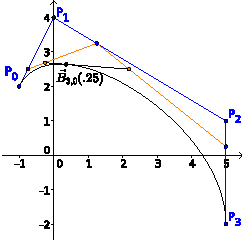
\includegraphics{figures/splines-parametric02a} 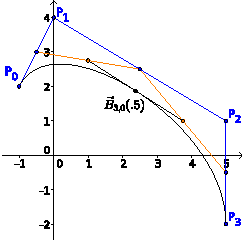
\includegraphics{figures/splines-parametric02b}
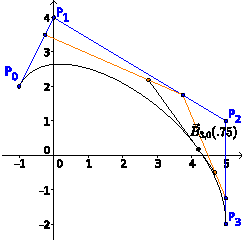
\includegraphics{figures/splines-parametric02c}
\par\end{centering}
\end{figure}
 \ref{fig:bezierViaLinearInterpolation} memperlihatkan kurva B\'ezier
ini beserta konstruksi tiga titiknya melalui interpolasi linear rekursif.
Titik-titik biru terletak di sepanjang kurva linear B\'ezier $\vec{B}_{1,0},\vec{B}_{1,1},\vec{B}_{1,2}$.
Titik-titik jingga terletak di sepanjang kurva B\'ezier kuadratik
$\vec{B}_{2,0}$ dan $\vec{B}_{2,1}$. Titik-titik hitam terletak
di sepanjang kurva B\'ezier kubik. Grafik kurva-kurva kuadratik tersebut
tidak ditampilkan agar gambar tidak menjadi terlalu rumit.

Gambar \ref{fig:bezierViaLinearInterpolation} dapat membantu Anda
memahami rekursi tersebut, tetapi yang mungkin lebih penting, membantu
Anda memahami hubungan antara titik-titik kontrol dan kurva B\'ezier.
Sebagai contoh, setelah diperiksa dengan saksama, Anda mungkin menduga
bahwa ruas garis $\vec{B}_{1,0}$ dan $\vec{B}_{1,2}$ bersinggungan
dengan kurva B\'ezier kubik $\vec{B}_{3,0}$ di $\vec{P}_{0}$ dan
$\vec{P}_{3}$, secara berturut-turut. Pemeriksaan saksama atas rumus-rumusnya
akan menegaskan hal tersebut.

Menurut rumus \ref{eq:bezierPart1} dan \ref{eq:bezierPart2}, kurva
B\'ezier berderajat paling tinggi tiga dengan titik-titik kontrol
$\vec{P}_{0},\vec{P}_{1},\vec{P}_{2},\vec{P}_{3}$ dihitung sebagai
berikut:
\begin{eqnarray*}
\vec{B}_{1,0}(t) & = & (1-t)\vec{P}_{0}+(t)\vec{P}_{1}\\
\vec{B}_{1,1}(t) & = & (1-t)\vec{P}_{1}+(t)\vec{P}_{2}\\
\vec{B}_{1,2}(t) & = & (1-t)\vec{P}_{2}+(t)\vec{P}_{3}
\end{eqnarray*}
sehingga
\begin{eqnarray*}
\vec{B}_{2,0}(t) & = & (1-t)\vec{B}_{1,0}(t)+(t)\vec{B}_{1,1}(t)=(1-t)\left[(1-t)\vec{P}_{0}+(t)\vec{P}_{1}\right]+t\left[(1-t)\vec{P}_{1}+(t)\vec{P}_{2}\right]\\
 & = & (1-t)^{2}\vec{P}_{0}+2t(1-t)\vec{P}_{1}+t^{2}\vec{P}_{2}\\
\vec{B}_{2,1}(t) & = & (1-t)\vec{B}_{1,1}(t)+(t)\vec{B}_{1,2}(t)=(1-t)\left[(1-t)\vec{P}_{1}+(t)\vec{P}_{2}\right]+t\left[(1-t)\vec{P}_{2}+(t)\vec{P}_{3}\right]\\
 & = & (1-t)^{2}\vec{P}_{1}+2t(1-t)\vec{P}_{2}+t^{2}\vec{P}_{3}
\end{eqnarray*}
sehingga
\begin{eqnarray}
\vec{B}_{3,0}(t) & = & (1-t)\vec{B}_{2,0}(t)+(t)\vec{B}_{2,1}(t)\nonumber \\
 & = & (1-t)\left[(1-t)^{2}\vec{P}_{0}+2t(1-t)\vec{P}_{1}+t^{2}\vec{P}_{2}\right]+t\left[(1-t)^{2}\vec{P}_{1}+2t(1-t)\vec{P}_{2}+t^{2}\vec{P}_{3}\right]\label{eq:bezierCubicGeneral}\\
 & = & (1-t)^{3}\vec{P}_{0}+3t(1-t)^{2}\vec{P}_{1}+3t^{2}(1-t)\vec{P_{2}}+t^{3}\vec{P}_{3}.\nonumber 
\end{eqnarray}
Dengan demikian, $\frac{d}{dt}\vec{B}_{3,0}(t)=-3(1-t)^{2}\vec{P}_{0}+3\left[(1-t)^{2}-2t(1-t)\right]\vec{P}_{1}+3\left[2t(1-t)-t^{2}\right]\vec{P}_{2}+3t^{2}\vec{P}_{3}$,
dan dari sini diperoleh
\begin{eqnarray*}
\left.\frac{d}{dt}\vec{B}_{3,0}(t)\right|_{t=0} & = & -3\vec{P}_{0}+3\vec{P}_{1}=3(\vec{P}_{1}-\vec{P}_{0})\\
\left.\frac{d}{dt}\vec{B}_{3,0}(t)\right|_{t=1} & = & -3\vec{P}_{2}+3\vec{P}_{3}=3(\vec{P}_{3}-\vec{P}_{2}).
\end{eqnarray*}
Memang, turunan $\vec{B}_{3,0}$ pada $0$ searah dengan ruas garis
dari $\vec{P}_{1}$ ke $\vec{P}_{2}$, dan turunan $\vec{B}_{3,0}$
pada $1$ searah dengan ruas garis dari $\vec{P}_{2}$ ke $\vec{P}_{3}$.
Selain itu, magnitudo turunan-turunan ini tepat tiga kali magnitudo
ruas-ruas garis tersebut.

Meskipun kita menempuh jalur yang agak berputar, kini kita melihat
cara lain untuk menghitung kurva B\'ezier kubik selain dengan menggunakan
rekursi \ref{eq:bezierPart1}/\ref{eq:bezierPart2} atau rumus \ref{eq:bezierCubicGeneral}.
Titik kontrol $\vec{P}_{0}$ dan $\vec{P}_{3}$ memberi kita dua titik
yang harus dilalui oleh $x$ dan $y$. Titik kontrol $\vec{P}_{1}$
dan $\vec{P}_{2}$ memberi kita $\dot{x}$ dan $\dot{y}$ pada kedua
titik tersebut. Dengan penentuan demikian, $x$ dan $y$ merupakan
polinom Hermite kubik! 

Tepatnya, misalkan $\vec{P}_{i}=(x_{i},y_{i})$ untuk $i=0,1,2,3$.
Maka, $x(t)$ adalah polinom Hermite kubik dengan $x(0)=x_{0}$, $\dot{x}(0)=3(x_{1}-x_{0})$,
$x(1)=x_{3}$, dan $\dot{x}(1)=3(x_{3}-x_{2})$; sedangkan $y(t)$
adalah polinom Hermite kubik dengan $y(0)=y_{0}$, $\dot{y}(0)=3(y_{1}-y_{0})$,
$y(1)=y_{3}$, dan $\dot{y}(1)=3(y_{3}-y_{2})$.

Kita tutup bagian ini dengan menghitung kurva B\'ezier dari $\begin{pmatrix}-1\\
2
\end{pmatrix}$ ke $\begin{pmatrix}5\\
-2
\end{pmatrix}$ melalui titik kontrol $\begin{pmatrix}0\\
4
\end{pmatrix}$ dan $\begin{pmatrix}5\\
1
\end{pmatrix}$ dengan menggunakan persamaan \ref{eq:HermiteCubicForHumans} dan
membandingkan hasilnya dengan \ref{eq:bezierCubicExample}. Dengan
$x(0)=-1$, $\dot{x}(0)=3$, $x(1)=5$, dan $\dot{x}(1)=0$ (dan substitusi
$x$ untuk $y$ yang dipahami), persamaan \ref{eq:HermiteCubicForHumans}
menghasilkan $m=\frac{5+1}{1-0}=6$ dan
\[
x(t)=\frac{t-1}{-1}(-1)+\frac{t}{1}(5)+\frac{(t-1)^{2}t}{1}\left(3-6\right)+\frac{t^{2}(t-1)}{1}\left(-6\right).
\]
Persamaan \ref{eq:HermiteCubicForHumans} dengan $y(0)=2$, $\dot{y}(0)=6$,
$y(1)=-2$, dan $\dot{y}(1)=-9$ menghasilkan $m=\frac{-2-2}{1-0}=-4$
dan
\[
y(t)=\frac{t-1}{-1}(2)+\frac{t}{1}(-2)+\frac{(t-1)^{2}t}{1}\left(6+4\right)+\frac{t^{2}(t-1)}{1}\left(-9+4\right).
\]
Walaupun persamaan-persamaan ini lengkap dan benar, sulit membandingkannya
dengan \ref{eq:bezierCubicExample} tanpa penyederhanaan. Dapatkah
Anda menunjukkan
\begin{eqnarray*}
x(t) & = & -1+3t+12t^{2}-9t^{3}\\
y(t) & = & 2+6t-15t^{2}+5t^{3}
\end{eqnarray*}
 sebagaimana disyaratkan? Jawaban \vpageref{ans:parametricCubics}.

\noindent\begin{digression}{Kurva B\'ezier dan CAGD}

\noindent Kurva B\'ezier pertama kali dikembangkan sekitar tahun
1960 oleh para pegawai perusahaan manufaktur otomotif Prancis. Paul
de Casteljau dari Citro\"en adalah yang pertama, tetapi Pierre B\'ezier
dari Renault memopulerkan metode ini sehingga namanya dikaitkan dengan
polinom-polinom tersebut.

Saat ini, hampir semua perangkat lunak desain grafis berbantuan komputer,
atau CAGD, menggunakan kurva B\'ezier, khususnya yang kubik, untuk
menggambar objek halus. Perangkat lunak CAGD dengan alat kurva B\'ezier
kubik akan menampilkan keempat titik kontrol dan memungkinkan pengguna
memindah-mindahkannya. Bahkan, perangkat lunak tersebut juga akan
menggambar dua kurva B\'ezier linear pada titik-titik ujung. Ini
memberi pengguna ``gagang kontrol'' untuk memanipulasi kurva. Beberapa
perangkat lunak juga akan menyertakan kurva B\'ezier linear ketiga.
Ketiga kurva linear B\'ezier tersebut bersama-sama membentuk apa
yang disebut poligon kontrol. Karena hubungan antara titik-titik kontrol
dan kurva bersifat intuitif, manipulasi titik-titik kontrol, baik
melalui gagang kontrol maupun poligon kontrol, menyediakan sarana
untuk memodelkan bentuk-bentuk halus dengan cepat. 

Namun, beberapa bentuk terlalu rumit untuk dimodelkan dengan satu
kurva B\'ezier kubik. Untuk menangani bentuk-bentuk seperti itu,
perangkat lunak CAGD memungkinkan pengguna merangkai kurva B\'ezier
kubik ujung ke ujung sehingga membentuk kurva B\'ezier komposit,
atau sepotong-sepotong, seperti yang ditampilkan di sini.

\begin{center}
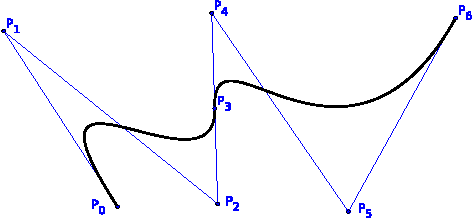
\includegraphics{figures/splines-parametric03}
\par\end{center}

\noindent Kurva ini terdiri atas dua kurva B\'ezier kubik, yang pertama
bertitik kontrol $\vec{P}_{0},\vec{P}_{1},\vec{P}_{2},\vec{P}_{3}$
dan yang kedua bertitik kontrol $\vec{P}_{3},\vec{P}_{4},\vec{P}_{5},\vec{P}_{6}$.
Karena kurva B\'ezier dimaksudkan untuk memodelkan objek halus, perangkat
lunak akan menyediakan opsi untuk memaksakan kecocokan turunan pada
titik bersama seperti $\vec{P}_{3}$. Hal ini dilakukan dengan memastikan
bahwa titik bersama berada pada ruas garis di antara dua titik kontrol
yang bersebelahan dengannya ($\vec{P}_{2}$ dan $\vec{P}_{4}$ pada
diagram ini). Anda dapat melihat versi interaktif diagram ini di \href{http://lqbrin.github.io/tea-time-numerical/ancillaries.html}{situs pendamping}.

Perangkat lunak bebas dan sumber terbuka seperti Inkscape, LibreOffice
Drawing, dan Dia menyediakan alat untuk menggambar kurva B�zier, tetapi
tidak semuanya menggunakan istilah teknis tersebut. Inkscape memiliki
alat kurva B�zier dengan nama itu, tetapi alat kurva B�zier pada LibreOffice
Drawing hanya disebut ``kurva'', sedangkan alat Dia yang hanya untuk
kurva B�zier tunggal, bukan komposit, bernama ``Bezierline''. 
\begin{description}
\item [{Referensi}] \cite{bezier,decasteljau,amsbezier,inkscape,dia,libreoffice}
\end{description}
\noindent\end{digression}

\subsection{Konsep Utama}
\begin{description}
\item [{polinom~oskulasi:}] Polinom yang grafiknya harus melalui sekumpulan
titik yang ditentukan 
\[
(x_{0},y_{0}),(x_{1},y_{1}),\ldots,(x_{n},y_{n})
\]
serta $m_{i}$ turunan pertamanya juga dapat ditentukan pada $x_{i}$.
\item [{polinom~Hermite:}] Polinom oskulasi yang harus melalui dua titik
dengan turunan pertamanya ditentukan pada setiap titik.
\item [{kurva~B\'ezier:}] Kurva yang menghubungkan dua titik melalui
polinom oskulasi parametrik.
\end{description}
\startexercises 

\subsection{Latihan}
\begin{enumerate}
\item Tentukan polinom Hermite kubik yang menginterpolasi data berikut.

\begin{center}
\begin{tabular}{c|cc}
$x$ & $f(x)$ & $f'(x)$\tabularnewline
\hline 
1 & 2 & 1\tabularnewline
5 & 3 & $-1$\tabularnewline
\end{tabular}
\par\end{center}
\item Tentukan polinom Hermite berderajat (paling tinggi) 5 yang menginterpolasi
data berikut.

\begin{center}
\begin{tabular}{c|cc}
$x$ & $f(x)$ & $f'(x)$\tabularnewline
\hline 
0 & 2 & 1\tabularnewline
$0.5$ & 2 & 0\tabularnewline
1 & 2 & 1\tabularnewline
\end{tabular}
\par\end{center}
\item Misalkan $g(x)=(\sqrt{2})^{x}$.

\begin{enumerate}
\item Dengan menggunakan $x_{0}=1$ dan $x_{1}=2$, tentukan polinom interpolasi
Hermite untuk $g$.
\item Gunakan polinom Hermite untuk menghampiri $g(1.5)$.
\item Hitung galat aktual dari hampiran ini, lalu bandingkan dengan galat
yang Anda peroleh pada soal \ref{exc:interpolation-lagrange-5} di
bagian \ref{sec:polynomialLagrange} \vpageref{exc:interpolation-lagrange-5}.
\item Polinom manakah yang menghampiri $g(1.5)$ dengan galat mutlak yang
lebih kecil, polinom Hermite atau polinom interpolasi Lagrange?
\end{enumerate}
\item Tentukan polinom yang melalui titik-titik $(0,0)$ dan $(4,-3)$ dan
yang turunannya melalui titik-titik $(0,1)$ dan $(4,1)$.
\item \label{data}Susun polinom interpolasi Hermite untuk data yang diberikan.
Lakukan ini dengan pensil, kertas dan kalkulator, atau lembar sebar.
Jangan gunakan kode Octave.

\begin{center}
\begin{tabular}{c|c|c}
$x$ & $f(x)$ & $f'(x)$\tabularnewline
\hline 
$0.1$ & $-0.29004996$ & $-2.8019975$\tabularnewline
$0.2$ & $-0.56079734$ & $-2.6159201$\tabularnewline
$0.3$ & $-0.81401972$ & $-2.4533949$\tabularnewline
\end{tabular}
\par\end{center}
\item Tentukan persamaan parametrik untuk kurva B\'ezier kubik. Ujung-ujung
``gagang kontrol'' adalah keempat titik kontrol.

\begin{center}
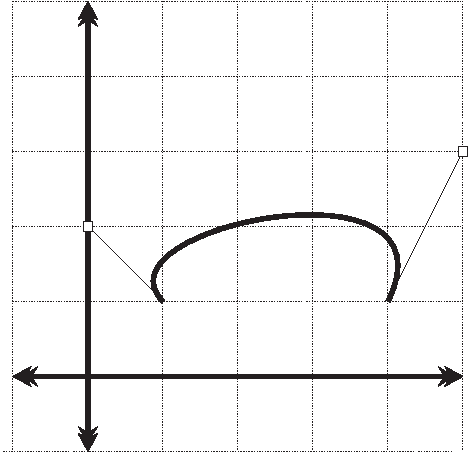
\includegraphics[scale=0.75]{figures/splines-parametric04}
\par\end{center}
\item Tuliskan persamaan parametrik kurva B\'ezier dengan titik-titik kontrol
$(-1,2)$, $(-3,2)$, $(3,1)$, dan $(3,0)$. Jawaban Anda tidak perlu
disederhanakan.
\item Susun persamaan parametrik untuk kurva B\'ezier dengan titik-titik
kontrol $(1,1),(2,1.5),(7,1.5),(6,2)$.
\item Tentukan persamaan polinom-polinom kubik yang membentuk kurva B\'ezier
komposit.

\begin{center}
\includegraphics[scale=0.6]{figures/splines-parametric06}
\par\end{center}
\item Data pada soal \ref{data} dihasilkan dengan menggunakan $f(x)=x^{2}\cos(x)-3x$.

\begin{enumerate}
\item \label{approximation}Hampiri $f(0.18)$ dengan menggunakan polinom
dari soal \ref{data}.
\item \label{error}Hitung galat mutlak dari hampiran ini.
\end{enumerate}
\item Misalkan $H(x)=x^{5}-3x^{4}+2x^{3}-6x+2$ merupakan polinom Hermite
yang menginterpolasi data

\begin{center}
\begin{tabular}{c|cc}
$x$ & $f(x)$ & $f'(x)$\tabularnewline
\hline 
0 & 2 & $-6$\tabularnewline
1 & $-4$ & \tabularnewline
2 & $-10$ & $2$\tabularnewline
\end{tabular}
\par\end{center}

diperoleh dari suatu fungsi $f$. Carilah datum yang hilang.
\item Suatu polinom Hermite $H(x)$ dikonstruksi menggunakan data

\begin{center}
\begin{tabular}{|c|c|c|c|c|}
\hline 
$x$ & $0.3$ & $0.5$ & $0.6$ & $0.8$\tabularnewline
\hline 
$f(x)$ & $0.8$ & $0.6$ & $0.3$ & $0.5$\tabularnewline
\hline 
$f'(x)$ & $1.5$ & $-1.2$ & $-5.3$ & $-2$\tabularnewline
\hline 
\end{tabular}
\par\end{center}
\begin{enumerate}
\item Carilah $(H\circ H)'(0.6)$. Dengan kata lain, carilah turunan dari
$H(H(x))$ yang dievaluasi pada $x=0.6$.
\item Carilah $(f\circ f)'(0.8)$.
\end{enumerate}
\item Polinom interpolasi Hermite untuk data berikut berbentuk $H(x)=a_{0}+a_{1}(x-0.3)+a_{2}(x-0.3)^{2}+\ldots$.

\begin{center}
\begin{tabular}{c|c|c}
$x$ & $f(x)$ & $f'(x)$\tabularnewline
\hline 
$0.30$ & $0.295$ & $-0.155$\tabularnewline
$0.32$ & $0.314$ & $-0.149$\tabularnewline
$0.35$ & $0.342$ & $-0.139$\tabularnewline
\end{tabular}
\par\end{center}
\begin{enumerate}
\item Isilah bagian yang hilang dalam bentuk $H(x)$.
\item Berapakah derajat maksimum yang mungkin untuk $H(x)$?
\item Carilah $a_{0}$ dan $a_{1}$.
\end{enumerate}
\item Konstruksikan tabel beda terbagi yang menghasilkan polinom Hermite
\[
p(x)=2-(x-1)+\frac{1}{4}(x-1)^{2}+\frac{1}{4}(x-1)^{2}(x-3).
\]
\item Kurva B\'ezier
\begin{eqnarray*}
x(t) & = & 11t^{3}-18t^{2}+3t+5\\
y(t) & = & t^{3}+1
\end{eqnarray*}
memiliki titik kontrol $(5,1)$, $(6,1)$, dan $(1,2)$. Carilah titik
kontrol keempat.
\item Berapakah jumlah minimum kurva B\'ezier kubik pada diagram tersebut,
dan mengapa?

\begin{center}
\includegraphics[scale=0.5]{figures/splines-parametric06}
\par\end{center}
\item Perhatikan grafik berikut.

\begin{center}
\includegraphics[scale=0.2]{figures/splines-parametric05}
\par\end{center}
\begin{enumerate}
\item Grafik tersebut tidak mungkin merupakan grafik satu kurva B\'ezier
kubik. Mengapa?
\item Grafik tersebut adalah grafik kurva B\'ezier kubik komposit. Setidaknya
berapa kurva B\'ezier kubik yang telah digabungkan, dan mengapa?
\end{enumerate}
\item Berikan tiga alasan yang dapat membuat Anda menggunakan kurva B\'ezier
alih-alih polinom Lagrange untuk memodelkan suatu grafik.
\item Polinom oskulasi $p(x)$ yang melalui $(x_{0},f(x_{0}))$ dengan $P'(x_{0})=f'(x_{0})$,
$P''(x_{0})=f''(x_{0})$, dan $P'''(x_{0})=f'''(x_{0})$ juga disebut
apa? Berikan jawaban sespesifik mungkin.
\item Kurva B\'ezier polar kubik merupakan satu-satunya fungsi polar kubik
(terparametrisasi) $(r(t),\theta(t))$ yang memenuhi data berikut.

\begin{center}
\begin{tabular}{|c|c|c|c|c|}
\hline 
$t$ & $r(t)$ & $\theta(t)$ & $\dot{r}(t)$ & $\dot{\theta(t)}$\tabularnewline
\hline 
$0$ & $r_{0}$ & $\theta_{0}$ & $\delta_{0}$ & $\mu_{0}$\tabularnewline
\hline 
$1$ & $r_{1}$ & $\theta_{1}$ & $\delta_{1}$ & $\mu_{1}$\tabularnewline
\hline 
\end{tabular}
\par\end{center}
\begin{enumerate}
\item Sebuah kurva B\'ezier kubik standar ditentukan oleh titik kontrol
$(0,0)$, $(2,0)$, $(0,1)$, dan $(0,3)$ (dalam urutan tersebut).
Konversikan data ini menjadi data koordinat polar. Ingatlah bahwa
konversi dari koordinat Kartesius ke koordinat polar melibatkan rumus
\[
r=\sqrt{x^{2}+y^{2}}\quad\mbox{dan}\quad\tan\theta=\frac{y}{x}.
\]
\item Carilah kurva B\'ezier polar kubik berdasarkan hasil Anda dari (a).
\end{enumerate}
\item \octave\ Tulislah fungsi Octave untuk menghitung polinom Hermite.
\item \octave\ Sebuah mobil yang melaju di sepanjang jalan lurus diukur
pada sejumlah titik. Data hasil pengamatan diberikan dalam tabel berikut,
dengan waktu dalam detik, jarak dalam kaki, dan kecepatan dalam kaki
per detik.

\begin{center}
\begin{tabular}{l|c|c|c|c|c}
Waktu & 0 & 3 & 5 & 8 & 13\tabularnewline
\hline 
Jarak & 0 & 225 & 383 & 623 & 993\tabularnewline
\hline 
Kecepatan & 75 & 77 & 80 & 74 & 72\tabularnewline
\end{tabular}
\par\end{center}
\begin{enumerate}
\item Hitunglah polinom interpolasi Hermite untuk data tersebut.
\item Gunakan polinom Anda dari bagian (a) untuk memprediksi posisi (jarak)
mobil dan kecepatannya pada saat $t=10$ detik.
\item Tentukan apakah mobil tersebut pernah melebihi batas kecepatan 55
mil per jam di jalan tersebut. Jika ya, kapan mobil tersebut pertama
kali melebihi kecepatan ini?
\item Berapakah prediksi kecepatan maksimum mobil tersebut?
\end{enumerate}
CATATAN: Kecepatan adalah turunan dari jarak. 
\begin{eqnarray*}
55\frac{\textrm{mil}}{\textrm{jam}} & = & 55\frac{\textrm{mil}}{\textrm{jam}}\times\frac{5280\textrm{ kaki}}{\textrm{mil}}\times\frac{1\textrm{ jam}}{3600\textrm{ detik}}\\
 & \approx & 80.67\frac{\textrm{kaki}}{\textrm{detik}}
\end{eqnarray*}

\item \octave\ Lengkapilah kode berikut.

\begin{lyxcode}
\#\#\#\#\#\#\#\#\#\#\#\#\#\#\#\#\#\#\#\#\#\#\#\#\#\#\#\#\#\#\#\#\#\#\#\#\#\#\#

\#~Written~by~Dr.~Len~Brin~~~~~~~~~~~~~\#

\#~13~March~2012~~~~~~~~~~~~~~~~~~~~~~~\#

\#~Purpose:~Evaluate~an~interpolating~~\#

\#~~~~~~polynomial~at~the~value~z.~~~~~\#

\#~INPUT:~number~z~~~~~~~~~~~~~~~~~~~~~\#

\#~~~~~~Data~x0,x1,...,xn~used~to~~~~~~\#

\#~~~~~~calculate~the~polynomial:~x~~~~\#

\#~~~~~~Entries~a0;0,~a1;0,1,~...~~~~~~\#

\#~~~~~~an;0,1,...,n~as~an~array:~c~~~~\#

\#~OUTPUT:~P(z),~the~value~of~the~~~~~~\#

\#~~~~~~interpolating~polynomial~at~z.~\#

\#\#\#\#\#\#\#\#\#\#\#\#\#\#\#\#\#\#\#\#\#\#\#\#\#\#\#\#\#\#\#\#\#\#\#\#\#\#\#

function~ans~=~divDiffEval(z,x,c)

~~n~=~length(x);

~~ans~=~c(n);

~~for~i=1:n-1

~~~~ans=(z-x(???)){*}ans+c(???);

~~end\#for

end\#function
\end{lyxcode}
\end{enumerate}
\finishexercises 

\subsection*{Jawaban}
\begin{description}
\item [{Bentuk~komputasi~polinom~Hermite:}] \label{ans:hermiteCoefficients}Empat
entri yang tersisa adalah
\begin{eqnarray*}
f_{1,1} & = & \frac{y_{1}-y_{0}}{t_{1}-t_{0}}\\
f_{0,2} & = & \frac{f_{1,1}-\dot{y}_{0}}{t_{1}-t_{0}}=\frac{y_{1}-y_{0}}{(t_{1}-t_{0})^{2}}-\frac{\dot{y}_{0}}{t_{1}-t_{0}}\\
f_{1,2} & = & \frac{\dot{y}_{1}-f_{1,1}}{t_{1}-t_{0}}=\frac{\dot{y}_{1}}{t_{1}-t_{0}}-\frac{y_{1}-y_{0}}{(t_{1}-t_{0})^{2}}\\
f_{0,3} & = & \frac{f_{1,2}-f_{0,2}}{t_{1}-t_{0}}=\frac{\dot{y}_{1}+\dot{y}_{0}}{(t_{1}-t_{0})^{2}}-2\frac{y_{1}-y_{0}}{(t_{1}-t_{0})^{3}}
\end{eqnarray*}
\item [{Kurva~B�zier~$\vec{B}_{j,i}(t)$~adalah~polinom~berderajat}] paling
tinggi $j$~yang~menghubungkan~$\vec{P_{i}}$~dengan~$\vec{P_{i+j}}$:
\label{ans:bezierProof}

\begin{proof}
Pembuktian dilakukan dengan induksi terhadap $j$, dimulai dari $j=1$:
Berdasarkan
\[
\vec{B}_{1,i}(t)=(1-t)\vec{P}_{i}+(t)\vec{P}_{i+1},\qquad i=0,1,\ldots,n-1,
\]
, berlaku $\vec{B}_{1,i}(0)=\vec{P}_{i}$ dan $B_{1,i}(1)=\vec{P}_{i+1}$,
sehingga $\vec{B}_{1,i}$ menghubungkan $\vec{P}_{i}$ dengan $\vec{P}_{i+1}$.
Selain itu, $\vec{B}_{1,i}(t)=\vec{P}_{i}+t(\vec{P}_{i+1}-\vec{P}_{i})$,
sehingga $\vec{B}_{1,i}$ merupakan polinom berderajat paling tinggi
1. Sekarang andaikan $\vec{B}_{j,i}(t)$ merupakan polinom berderajat
paling tinggi $j$ yang menghubungkan $\vec{P_{i}}$ dengan $\vec{P_{i+j}}$
untuk suatu $j\geq1$ (dan semua $i$ yang berlaku). Berdasarkan definisi,
$\vec{B}_{j+1,i}(0)=\vec{B}_{j,i}(0)$ dan $\vec{B}_{j+1,i}(1)=\vec{B}_{j,i+1}(1)$.
Berdasarkan hipotesis induksi, $\vec{B}_{j,i}(0)=\vec{P}_{i}$ dan
$\vec{B}_{j,i+1}(1)=\vec{P}_{i+j+1}$, sehingga $\vec{B}_{j+1,i}$
menghubungkan $\vec{P}_{i}$ dengan $\vec{P}_{i+j+1}$. Selain itu,
\[
\vec{B}_{j+1,i}(t)=(1-t)\cdot\vec{B}_{j,i}(t)+(t)\cdot\vec{B}_{j,i+1}(t)
\]
berderajat paling tinggi $j+1$ karena $\vec{B}_{j,i}(t)$ dan $\vec{B}_{j,i+1}(t)$
masing-masing berderajat paling tinggi $j$ (berdasarkan hipotesis
induksi). Dengan demikian, pembuktian selesai.
\end{proof}
\item [{Kurva}] B\'ezier~melalui~polinom~Hermite~kubik: \label{ans:parametricCubics}Penyederhanaannya
dapat dilakukan sebagai berikut.
\begin{eqnarray*}
x(t) & = & \frac{t-1}{-1}(-1)+\frac{t}{1}(5)+\frac{(t-1)^{2}t}{1}\left(3-6\right)+\frac{t^{2}(t-1)}{1}\left(-6\right)\\
 & = & (t-1)+5t-3t(t-1)^{2}-6t^{2}(t-1)\\
 & = & 6t-1-3t(t^{2}-2t+1)-6t^{3}+6t^{2}\\
 & = & 6t-1-3t^{3}+6t^{2}-3t-6t^{3}+6t^{2}\\
 & = & -9t^{3}+12t^{2}+3t-1
\end{eqnarray*}
dan
\begin{eqnarray*}
y(t) & = & \frac{t-1}{-1}(2)+\frac{t}{1}(-2)+\frac{(t-1)^{2}t}{1}\left(6+4\right)+\frac{t^{2}(t-1)}{1}\left(-9+4\right)\\
 & = & -2(t-1)-2t+10t(t-1)^{2}-5t^{2}(t-1)\\
 & = & -2t+2-2t+10t(t^{2}-2t+1)-5t^{3}+5t^{2}\\
 & = & 2-4t+10t^{3}-20t^{2}+10t-5t^{3}+5t^{2}\\
 & = & 5t^{3}-15t^{2}+6t+2.
\end{eqnarray*}
\end{description}




\section{Splin\label{sec:Splines}}

Polinom oskulasi memiliki kegunaan terbatas dalam aplikasi yang mengharuskan
suatu kurva melalui sejumlah besar titik. Dan jumlah besar mungkin
hanya berarti sekitar \textit{setengah lusin}. Perhatikan himpunan
titik yang tampak biasa berikut ini.

\begin{center}
\includegraphics[width=7.5cm]{figures/generalizedSplines01}
\par\end{center}

\noindent Mudah untuk membayangkan suatu fungsi yang tampak sama sederhananya
dan melalui titik ini, tetapi mencari fungsi tersebut ternyata sedikit
menantang. Polinom interpolasi berderajat terendah berosilasi terlalu
lebar.

\begin{center}
\includegraphics[width=7.5cm]{figures/generalizedSplines02}
\par\end{center}

\noindent Ini merupakan masalah umum pada polinom interpolasi berderajat
tinggi. Tidak ada kendali terhadap osilasinya, dan osilasi tersebut
biasanya tidak diinginkan. Osilasinya dapat diredam sampai tingkat
tertentu dengan mencari polinom oskulasi yang melalui titik-titik
ini dengan, misalnya, turunan pertama sebesar $0$ pada $0$ dan sebesar
$-\frac{1}{2}$ pada titik ketujuh dari kiri (titik yang koordinat
$x$-nya berada di antara 5 dan 6).

\begin{center}
\includegraphics[width=7.5cm]{figures/generalizedSplines03}
\par\end{center}

\noindent Itu lebih baik, tetapi masih belum sepenuhnya memuaskan.
Menetapkan turunan pertama pada dua titik semata-mata untuk mengurangi
osilasi juga agak sewenang-wenang---lebih baik membiarkan sifat masalah
yang menentukan. Osilasi pada percobaan sebelumnya membuat hasilnya
terlalu khas dan menarik bagi himpunan titik hambar yang menjadi titik
awal kita. Cara yang sepantasnya sederhana untuk menginterpolasi data
tersebut adalah menghubungkan titik-titik berurutan dengan ruas garis.

\begin{center}
\includegraphics[width=7.5cm]{figures/generalizedSplines04}
\par\end{center}

\noindent Ini membentuk apa yang dikenal sebagai interpolasi linear
sepotong-sepotong dari himpunan data tersebut. Jenis grafik ini sering
terlihat di media massa. Namun, banyak aplikasi, terutama yang berasal
dari bidang teknik, memerlukan suatu tingkat kehalusan. Menghubungkan
setiap tiga titik berurutan dengan fungsi kuadratik dapat membantu.

\begin{center}
\includegraphics[width=7.5cm]{figures/generalizedSplines05}
\par\end{center}

\noindent Hal itu menjamin kehalusan pada tiga titik, tetapi fungsi
tersebut masih belum terdiferensialkan pada titik-titik yang dipakai
bersama oleh fungsi kuadratik berurutan. Selain itu, menggunakan tiga
titik pertama untuk fungsi kuadratik pertama (yang tampak linear bagi
mata telanjang), titik ketiga sampai kelima untuk fungsi kuadratik
kedua, dan titik kelima sampai ketujuh untuk fungsi kuadratik ketiga
(yang juga tampak linear bagi mata telanjang) hanya menyisakan titik
ketujuh dan kedelapan untuk fungsi yang semestinya merupakan fungsi
kuadratik keempat. Namun, karena hanya ada dua titik, sebagai gantinya
digunakan ruas garis. Solusi yang lebih halus adalah memastikan bahwa
turunan pertama fungsi kuadratik berurutan cocok pada titik bersama.
Dengan gagasan ini, masuk akal untuk mencocokkan hanya dua titik dengan
setiap parabola, sehingga tersisa satu koefisien (dari tiga pada setiap
fungsi kuadratik) untuk mencocokkan turunan fungsi kuadratik tetangganya.

\begin{center}
\includegraphics[width=7.5cm]{figures/generalizedSplines06}
\par\end{center}

\noindent Itu lebih baik! Fungsi parabola sepotong-sepotong ini memiliki
turunan pertama yang kontinu, tetapi masih ada sesuatu yang sewenang-wenang.
Ketujuh parabola itu secara keseluruhan memiliki 21 koefisien. Membuat
setiap parabola melalui dua titik memberikan 14 syarat pada koefisien-koefisien
tersebut. Mencocokkan turunan pertama parabola-parabola yang berdampingan
pada titik bersama memberikan 6 syarat lagi, satu pada masing-masing
dari 6 titik interior. Hal ini menyisakan satu koefisien ``bebas''.
Menetapkan satu syarat terakhir tampak agak sewenang-wenang, dan memang
demikian. Grafik menunjukkan hasil ketika turunan pada $0$ ditetapkan
menjadi $1$. Perhatikan bahwa tidak ada kendali terhadap turunan
di ujung kanan. Selain sifatnya yang sewenang-wenang, ketidaksimetrian
ini mengganggu. Andaikan kita memiliki satu derajat kebebasan lagi...

\subsection{Polinom sepotong-sepotong}

Suatu fungsi yang didefinisikan sepotong-sepotong dan semua potongannya
berupa polinom disebut polinom sepotong-sepotong. Bentuknya adalah
\[
p(x)=\begin{cases}
p_{1}(x), & x\in[x_{0},x_{1}]\\
p_{2}(x), & x\in(x_{1},x_{2}]\\
 & \vdots\\
p_{n}(x) & x\in(x_{n-1},x_{n}]
\end{cases}
\]
dengan $p_{i}(x)$ merupakan polinom untuk setiap $i=1,2,\ldots,n$
dan $x_{0}<x_{1}<\cdots<x_{n}$; atau suatu varian yang membuat $p(x_{j})$
didefinisikan oleh tepat satu dari $p_{i}$. Jika setiap $p_{i}$
merupakan fungsi linear, $p$ disebut linear sepotong-sepotong. Jika
setiap $p_{i}$ merupakan fungsi kuadratik, $p$ disebut kuadratik
sepotong-sepotong. Jika setiap $p_{i}$ merupakan fungsi kubik, $p$
disebut kubik sepotong-sepotong. Demikian seterusnya. Contoh fungsi
linear sepotong-sepotong dan kuadratik sepotong-sepotong terdapat
pada pendahuluan bagian ini.

\subsection{Splin}

Definisi polinom sepotong-sepotong sama sekali tidak mengharuskan
fungsi tersebut terdiferensialkan atau bahkan kontinu. Fungsi berikut
merupakan polinom sepotong-sepotong.

\begin{center}
\includegraphics[width=7.5cm]{figures/generalizedSplines07}
\par\end{center}

\noindent Namun, sebagian besar aplikasi polinom sepotong-sepotong
memerlukan kekontinuan atau keterdiferensialan. Setiap polinom sepotong-sepotong
dengan sedikitnya satu turunan kontinu disebut splin. Titik-titik
yang memisahkan potongan-potongan yang berdampingan, yaitu $x_{j}$,
untuk $j=1,2,\ldots,n-1$, disebut simpul atau sambungan.

Grafik terakhir pada pendahuluan bagian ini memperlihatkan splin kuadratik.
Setiap potongan fungsi sepotong-sepotong tersebut merupakan fungsi
kuadratik, dan fungsi-fungsi kuadratik itu dipilih agar turunannya
cocok pada sambungan. Namun, seperti yang telah dinyatakan di sana,
kita perlu memberikan satu syarat yang tidak alami---turunan pada
titik ujung kiri. Syarat itu dapat berupa turunan pada titik mana
pun, atau bahkan turunan kedua pada salah satu titik. Dalam arti yang
sangat nyata, pilihan tersebut sewenang-wenang. Pilihan itu tidak
ditentukan secara alami oleh masalah yang dihadapi. Akibatnya, terdapat
suatu keluarga solusi untuk masalah menghubungkan delapan titik tersebut
dengan fungsi kuadratik sepotong-sepotong yang terdiferensialkan secara
kontinu.

\subsection{Splin kubik}

Splin yang paling umum digunakan adalah splin kubik. Seperti pada
splin kuadratik, splin kubik dihitung dengan mencocokkan turunan pada
sambungan. Bahkan, himpunan fungsi kubik memiliki cukup banyak koefisien
sehingga turunan pertama maupun kedua dapat dicocokkan. Namun, perhatikan
bahwa menurut definisi splin kita, pencocokan turunan pertama dan
kedua pada sambungan tidak sepenuhnya diperlukan. Sumber lain akan
memberikan definisi splin yang lebih ketat, yang mengharuskan pencocokan
kedua turunan tersebut. Sebagai konvensi, kita berfokus pada splin
seperti itu.

Splin kubik yang harus menginterpolasi $n+1$ titik memiliki $n-1$
sambungan dan $n$ potongan. Oleh karena itu, himpunan fungsi kubik
tersebut memiliki $4n$ koefisien. Mengharuskan setiap fungsi kubik
melalui $2$ titik menghasilkan $2n$ syarat pada koefisien. Mengharuskan
turunan pertama cocok pada sambungan memberikan $n-1$ syarat lagi.
Mengharuskan turunan kedua cocok pada sambungan memberikan tambahan
$n-1$ syarat, sehingga jumlah keseluruhannya adalah $4n-2$ syarat.
Hal ini menyisakan $2$ koefisien ``bebas''. Secara matematis, kita
memiliki suatu keluarga splin dengan dua derajat kebebasan. Untuk
memperoleh suatu splin tertentu, kita perlu memberlakukan dua syarat
lagi pada koefisien. Syarat-syarat ini dapat berupa turunan pertama,
kedua, atau ketiga pada dua simpul; turunan pertama dan kedua pada
satu simpul; atau kombinasi lain dari dua persyaratan turunan.

Mungkin dengan berpedoman pada pengetahuan tentang splin juru gambar,
konvensi mengarahkan kita untuk menetapkan syarat titik ujung. Artinya,
kita mensyaratkan sesuatu mengenai suatu turunan di $x_{0}$ dan di
$x_{n}$. Menentukan turunan pertama serupa dengan mengarahkan splin
juru gambar ke arah tertentu pada kedua ujungnya. Menetapkan turunan
kedua sama dengan $0$ serupa dengan membiarkan kedua ujung splin
juru gambar menunjuk bebas ke arah mana pun yang dibawa oleh hukum
fisika. Model splin juru gambar ini tidak terlalu akurat, tetapi memberikan
motivasi. 

Splin kubik yang turunan pertamanya ditentukan pada kedua titik ujung
disebut splin terapit. Splin kubik yang turunan keduanya ditetapkan
sama dengan nol pada kedua titik ujung disebut splin alami atau bebas.
Bentuk hibrida yang turunan pertamanya ditentukan pada satu ujung
dan turunan keduanya ditetapkan nol pada ujung lainnya tidak memiliki
nama khusus. Secara tepat, kita memiliki definisi berikut.

Misalkan $(x_{0},y_{0}),(x_{1},y_{1}),\ldots,(x_{n},y_{n})$ adalah
$n+1$ titik dengan $x_{0}<x_{1}<\cdots<x_{n}$, dan misalkan $S_{i}(x)=a_{i}+b_{i}(x-x_{i})+c_{i}(x-x_{i})^{2}+d_{i}(x-x_{i})^{3}$
untuk $i=1,2,\ldots,n$. Maka $S$, yang didefinisikan oleh 
\[
S(x)=\begin{cases}
S_{1}(x), & x\in[x_{0},x_{1}]\\
S_{2}(x), & x\in[x_{1},x_{2}]\\
 & \vdots\\
S_{n}(x), & x\in[x_{n-1},x_{n}]
\end{cases},
\]
merupakan splin kubik jika memenuhi tiga syarat berikut.
\begin{enumerate}
\item $S_{i}(x_{i-1})=y_{i-1}$ dan $S_{i}(x_{i})=y_{i}$ untuk $i=1,2,\ldots,n$
(interpolasi)
\item $S_{i}'(x_{i})=S_{i+1}'(x_{i})$ dan $S_{i}''(x_{i})=S_{i+1}''(x_{i})$
untuk $i=1,2,\ldots,n-1$ (pencocokan turunan)
\item Salah satu dari syarat berikut dipenuhi (syarat titik ujung)

\begin{enumerate}
\item \label{enu:naturalSpline}$S_{1}''(x_{0})=S_{n}''(x_{n})=0$
\item \label{enu:clampedSpline}$S_{1}'(x_{0})=m_{0}$ dan $S_{n}'(x_{n})=m_{n}$
untuk suatu $m_{0}$ dan $m_{n}$
\item \label{enu:mixed}$S_{1}'(x_{0})=m_{0}$ untuk suatu $m_{0}$ dan
$S_{n}''(x_{n})=0$
\item $S_{1}''(x_{0})=0$ dan $S_{n}'(x_{n})=m_{n}$ untuk suatu $m_{n}$
\end{enumerate}
\end{enumerate}
Jika kondisi titik ujung \ref{enu:naturalSpline} dipenuhi, $S$ disebut
splin bebas atau splin alami. Jika kondisi titik ujung \ref{enu:clampedSpline}
dipenuhi, $S$ disebut splin terapit.

Splin (kubik) alami yang melalui delapan titik yang disajikan dalam
pendahuluan bagian ini tampak seperti berikut. 

\begin{center}
\includegraphics[width=7.5cm]{figures/generalizedSplines08}
\par\end{center}

\noindent Akhirnya, sebuah fungsi yang sama tidak istimewanya dengan
himpunan datanya! Bagaimana cara menghitungnya, Anda bertanya? Jawaban
singkatnya: 28 persamaan simultan yang dihasilkan dari definisi splin
kubik alami diselesaikan. Penyelesaiannya memberikan koefisien $a_{i},b_{i},c_{i},d_{i}$,
$i=1,2,\ldots,7$.

\subsubsection{Menyusun persamaan}

Jawaban panjangnya memang agak lebih panjang untuk diuraikan, tetapi
sebenarnya hanya berbeda dari versi singkat dalam tingkat kerinciannya.
Sebagai langkah awal, syarat $S_{i}(x_{i})=y_{i}$ langsung memberi
kita nilai bagi $n$ koefisien:
\[
S_{i}(x_{i})=a_{i}=y_{i}.
\]
Syarat $S_{i}(x_{i-1})=y_{i-1}$ memberi kita $n$ persamaan
\begin{equation}
S_{i}(x_{i-1})=y_{i}+b_{i}(x_{i-1}-x_{i})+c_{i}(x_{i-1}-x_{i})^{2}+d_{i}(x_{i-1}-x_{i})^{3}=y_{i-1}\label{eq:interpolationRequirement}
\end{equation}
untuk $i=1,2,\ldots,n$. Masing-masing syarat turunan memberi kita
$n-1$ persamaan:
\begin{eqnarray}
S_{i}'(x_{i})=S_{i+1}'(x_{i}) & \Rightarrow & b_{i}=b_{i+1}+2c_{i+1}(x_{i}-x_{i+1})+3d_{i+1}(x_{i}-x_{i+1})^{2}\label{eq:firstDerivativeRequirement}\\
S_{i}''(x_{i})=S_{i+1}''(x_{i}) & \Rightarrow & 2c_{i}=2c_{i+1}+6d_{i+1}(x_{i}-x_{i+1})\label{eq:secondDerivative Requirement}
\end{eqnarray}
untuk $i=1,2,\ldots,n-1$. Terakhir, kondisi titik ujung memberi kita
dua persamaan
\begin{eqnarray}
S_{1}''(x_{0}) & = & 2c_{1}+6d_{1}(x_{0}-x_{1})=0\label{eq:freeLeftEndpoint}\\
S_{n}''(x_{n}) & = & 2c_{n}=0.\label{eq:freeRightEndpoint}
\end{eqnarray}
Tanpa banyak kesulitan, kita memperoleh nilai $a_{i}$ dan $c_{n}$.
Sisa $3n-1$ koefisien diperoleh dengan menyelesaikan sisa $3n-1$
persamaan simultan. Meskipun komputer tentu dapat menangani penyelesaiannya
mulai dari tahap ini, menurunkan sebagian dari penyelesaian umum secara
manual menghasilkan algoritma yang jauh lebih efisien.

\subsubsection{Menyelesaikan persamaan}

Pada dasarnya, sekarang kita memiliki tiga persamaan dengan tiga peubah
tak diketahui. Persamaan \ref{eq:interpolationRequirement}, \ref{eq:firstDerivativeRequirement},
dan \ref{eq:secondDerivative Requirement} dituliskan dalam peubah
$b_{i},c_{i},d_{i}$. Persamaan \ref{eq:secondDerivative Requirement}
dapat dengan mudah diselesaikan untuk $d_{i}$ sebagai fungsi dari
$c_{i}$ dan persamaan \ref{eq:interpolationRequirement} dapat dengan
mudah diselesaikan untuk $b_{i}$. Ekspresi yang dihasilkan dapat
disubstitusikan ke dalam persamaan \ref{eq:firstDerivativeRequirement}
sehingga diperoleh persamaan yang hanya memuat $c_{i}$. Perhitungannya
dapat diselesaikan dengan mudah. Pada tahap ini, akan lebih mudah
jika kita mendefinisikan $h_{i}=x_{i-1}-x_{i}$. 
\begin{eqnarray}
(\mbox{\ref{eq:secondDerivative Requirement}}) & \Rightarrow & d_{i+1}=\frac{c_{i}-c_{i+1}}{3h_{i+1}},\quad i=1,2,\ldots,n-1\nonumber \\
 & \Rightarrow & d_{i}=\frac{c_{i-1}-c_{i}}{3h_{i}},\quad i=2,3,\ldots,n.\label{eq:di}\\
(\mbox{\ref{eq:interpolationRequirement}}) & \Rightarrow & b_{i}=\frac{y_{i-1}-y_{i}}{h_{i}}-c_{i}h_{i}-d_{i}h_{i}^{2},\quad i=1,2,\ldots,n\nonumber \\
 & \Rightarrow & b_{i}=\frac{y_{i-1}-y_{i}}{h_{i}}-c_{i}h_{i}-\frac{(c_{i-1}-c_{i})h_{i}}{3},\quad i=2,3,\ldots,n\nonumber \\
 & \Rightarrow & b_{i}=\frac{y_{i-1}-y_{i}}{h_{i}}-\frac{(c_{i-1}+2c_{i})h_{i}}{3},\quad i=2,3,\ldots,n\label{eq:bi}\\
 & \Rightarrow & b_{i+1}=\frac{y_{i}-y_{i+1}}{h_{i+1}}-\frac{(c_{i}+2c_{i+1})h_{i+1}}{3},\quad i=1,2,\ldots,n-1.\nonumber 
\end{eqnarray}
Menyubstitusikan ekspresi tersebut ke dalam persamaan \ref{eq:firstDerivativeRequirement}
menghasilkan
\[
\frac{y_{i-1}-y_{i}}{h_{i}}-\frac{(c_{i-1}+2c_{i})h_{i}}{3}=\frac{y_{i}-y_{i+1}}{h_{i+1}}-\frac{(c_{i}+2c_{i+1})h_{i+1}}{3}+2c_{i+1}h_{i+1}+(c_{i}-c_{i+1})h_{i+1}
\]
untuk $i=2,3,\ldots,n-1$. Dengan sedikit penyederhanaan, persamaan
ini menjadi
\begin{equation}
h_{i}c_{i-1}+2(h_{i}+h_{i+1})c_{i}+h_{i+1}c_{i+1}=3\left(\frac{y_{i-1}-y_{i}}{h_{i}}-\frac{y_{i}-y_{i+1}}{h_{i+1}}\right),\quad i=2,3,\ldots,n-1.\label{eq:firstNm2}
\end{equation}
Kini kita memiliki $n-2$ persamaan dalam $n$ peubah tak diketahui
$c_{i}$. Persamaan-persamaan ini berlaku untuk sebarang splin kubik
dengan kondisi titik ujung apa pun. Namun, persamaan \ref{eq:firstDerivativeRequirement}
belum digunakan dengan indeks $i=1$. Karena itu, kita masih harus
memasukkan
\begin{equation}
b_{1}=b_{2}+2c_{2}h_{2}+3d_{2}h_{2}^{2}\label{eq:lastEquation}
\end{equation}
ke dalam penyelesaian. Tinggal mengganti $b_{1}$, $b_{2}$, dan $d_{2}$
dengan ekspresi dalam $c_{i}$. 

Sebagai langkah awal, persamaan \ref{eq:bi} dan \ref{eq:di} dengan
$i=2$ memberi
\begin{eqnarray*}
b_{2} & = & \frac{y_{1}-y_{2}}{h_{2}}-\frac{(c_{1}+2c_{2})h_{2}}{3}\\
d_{2} & = & \frac{c_{1}-c_{2}}{3h_{2}}.
\end{eqnarray*}
Dengan menyubstitusikan $b_{2}$ dan $d_{2}$, persamaan \ref{eq:lastEquation}
menjadi 
\begin{eqnarray}
b_{1} & = & \frac{y_{1}-y_{2}}{h_{2}}-\frac{(c_{1}+2c_{2})h_{2}}{3}+2c_{2}h_{2}+(c_{1}-c_{2})h_{2}\nonumber \\
 & = & \frac{y_{1}-y_{2}}{h_{2}}+\frac{2}{3}h_{2}c_{1}+\frac{1}{3}h_{2}c_{2}.\label{eq:b1}
\end{eqnarray}
Kita belum menggunakan kondisi titik ujung, sehingga persamaan ini
berlaku untuk sebarang splin kubik. Kondisi titik ujung apa pun yang
diberikan harus menghasilkan suatu ekspresi untuk $b_{1}$ sebagai
fungsi dari $c_{i}$ serta satu persamaan lain dalam $c_{i}$.

Untuk splin bebas, kondisi titik ujung \ref{eq:freeRightEndpoint}
memberi $c_{n}=0$. Ini adalah persamaan pertama dari dua persamaan
terakhir. Kondisi titik ujung \ref{eq:freeLeftEndpoint} memberi $d_{1}=-\frac{c_{1}}{3h_{1}}$.
Hubungan ini tidak langsung berguna karena kita sedang mencari ekspresi
untuk $b_{1}$. Namun, persamaan \ref{eq:interpolationRequirement}
dengan $i=1$ memberi $b_{1}=\frac{y_{0}-y_{1}}{h_{1}}-c_{1}h_{1}-d_{1}h_{1}^{2}$
sehingga kita dapat menggunakannya untuk memperoleh 
\begin{eqnarray*}
b_{1} & = & \frac{y_{0}-y_{1}}{h_{1}}-\frac{2}{3}c_{1}h_{1}.
\end{eqnarray*}
Terakhir, substitusi ke dalam persamaan \ref{eq:b1} menghasilkan
persamaan terakhir dalam $c_{i}$ adalah $\frac{y_{0}-y_{1}}{h_{1}}-\frac{2}{3}c_{1}h_{1}=\frac{y_{1}-y_{2}}{h_{2}}+\frac{2}{3}h_{2}c_{1}+\frac{1}{3}h_{2}c_{2}$,
yang dapat disederhanakan menjadi
\begin{equation}
2(h_{1}+h_{2})c_{1}+h_{2}c_{2}=3\left(\frac{y_{0}-y_{1}}{h_{1}}-\frac{y_{1}-y_{2}}{h_{2}}\right).\label{eq:finalEquation}
\end{equation}
Persamaan \ref{eq:firstNm2}, \ref{eq:finalEquation}, dan $c_{n}=0$
merupakan $n$ persamaan yang dapat diselesaikan untuk memperoleh
$n$ koefisien $c_{i}$. Substitusi balik akan memberikan nilai $b_{i}$
dan $d_{i}$.

Kondisi titik ujung lainnya menghasilkan pasangan persamaan akhir
yang berbeda, tetapi prosesnya sama. Kita perlu menyubstitusikan suatu
ekspresi untuk $b_{1}$ ke dalam \ref{eq:b1} dan menurunkan satu
persamaan lain.

\subsection{Kode Octave untuk Splin Alami}

Menghitung splin untuk tiga atau empat titik dapat dilakukan secara
manual dengan sedikit kesabaran dan ketelitian, tetapi bila jumlah
titik jauh lebih banyak, aljabarnya menjadi terlalu melelahkan. Namun,
setiap persamaan yang memuat $c_{i}$ hanya melibatkan paling banyak
tiga peubah $c_{i}$ sekaligus dan mengikuti pola teratur, setidaknya
untuk $n-2$ persamaan tersebut. Ciri-ciri ini membuat otomatisasi
penyelesaiannya cukup mudah. Kode berikut mungkin bukan yang paling
efisien untuk menentukan splin alami, tetapi disajikan demikian karena
dua alasan. Pertama, kode ini dimaksudkan untuk meniru secara saksama
penyelesaian aljabar yang diuraikan pada bagian sebelumnya sehingga
lebih mudah diikuti. Kedua, kode ini dimaksudkan cukup umum sehingga
modifikasinya untuk kondisi titik ujung lain hanya memerlukan sedikit
usaha. Latihan nanti akan meminta modifikasi semacam itu.

\noindent\begin{verbatim}
%%%%%%%%%%%%%%%%%%%%%%%%%%%%%%%%%%%%%%%%%%%%%%%%%
% Written by Dr. Len Brin           3 June 2014 %
% Purpose: Calculation of a natural cubic       %
%        spline.                                %
% INPUT: points (x(1),y(1)), (x(2),y(2)), ...   %
%        spline must interpolate.               %
% OUTPUT: coefficients of each piece of the     %
%        piecewise cubic spline:                %
%        S(i,x) = a(i)                          %
%          + b(i)*(x-x(i+1))                    %
%          + c(i)*(x-x(i+1))^2                  %
%          + d(i)*(x-x(i+1))^3                  %
%%%%%%%%%%%%%%%%%%%%%%%%%%%%%%%%%%%%%%%%%%%%%%%%%
function [a,b,c,d] = naturalCubicSpline(x,y)
  n=length(x)-1;
  for i=1:n
    h(i)=x(i)-x(i+1);
  end%for
  % Left endpoint condition:
  % m(1,1)*c(1) + m(1,2)*c(2) = m(1,n+1)
  m(1,1)=2*(h(1)+h(2)); m(1,2)=h(2);
  m(1,n+1)=3*((y(1)-y(2))/h(1)-(y(2)-y(3))/h(2));
  % Right endpoint condition:
  % m(n,n-1)*c(n-1) + m(n,n)*c(n) = m(n,n+1)
  m(n,n-1)=0; m(n,n)=1; m(n,n+1)=0;
  % Conditions for all splines:
  for i=2:n-1
    m(i,i-1)=h(i);
    m(i,i)=2*(h(i)+h(i+1));
    m(i,i+1)=h(i+1);
    m(i,n+1)=3*((y(i)-y(i+1))/h(i)-(y(i+1)-y(i+2))/h(i+1));
  end%for
  % Solve for c(i)
  l(1)=m(1,1); u(1)=m(1,2)/l(1); z(1)=m(1,n+1)/l(1);
  for i=2:n-1
    l(i)=m(i,i)-m(i,i-1)*u(i-1);
    u(i)=m(i,i+1)/l(i);
    z(i)=(m(i,n+1)-m(i,i-1)*z(i-1))/l(i);
  end%for
  l(n)=m(n,n)-m(n,n-1)*u(n-1);
  c(n)=(m(n,n+1)-m(n,n-1)*z(n-1))/l(n);
  for i=n-1:-1:1
    c(i)=z(i)-u(i)*c(i+1);
  end%for
  % Compute a(i), b(i), d(i)
  % Endpoint conditions:
  b(1)=(y(1)-y(2))/h(1)-2*c(1)*h(1)/3;
  d(1)=-c(1)/(3*h(1));
  % Conditions for all splines:
  a(1)=y(2);
  for i=2:n
    d(i)=(c(i-1)-c(i))/(3*h(i));
    b(i)=(y(i)-y(i+1))/h(i)-(c(i-1)+2*c(i))*h(i)/3;
    a(i)=y(i+1);
  end%for
end%function
\end{verbatim}\texttt{naturalCubicSpline.m} dapat diunduh dari \href{http://lqbrin.github.io/tea-time-numerical/ancillaries.html}{situs pendamping}.

\subsection{Penerapan Splin Kubik Alami?}

``Untuk banyak penerapan penting, model matematis {[}splin kubik{]}
bagi bilah lentur juru gambar ini sangat realistis.''\footnote{Ahlberg and Nilson, The Theory of Splines and their Applications,
Elsevier, 1967.} Klaim semacam ini bertumpu pada asumsi bahwa bilah lentur juru gambar
dapat dimodelkan dengan tepat sebagai balok tipis dan bahwa lendutan
balok kecil. Namun, bentuk yang dimodelkan oleh splin sering mencakup
lendutan besar, dan kecuali bilah lentur juru gambar rusak dalam suatu
cara, bentuknya akan berupa kurva yang terdiferensialkan tak hingga
kali. Turunan ketiga splin kubik pada umumnya tidak kontinu sehingga
splin tersebut tidak memiliki turunan berorde lebih tinggi. Selain
itu, kondisi titik ujung $S_{0}''(x_{0})=S_{n}''(x_{n})=0$ tidak
sesuai dengan situasi fisik tersebut. Kondisi-kondisi ini menyiratkan
bahwa bentuk splin memiliki kelengkungan (kecekungan) nol pada titik-titik
ujung, padahal tidak ada sesuatu pun dalam situasi fisik tersebut
yang mengarah pada kesimpulan itu.

Meskipun tidak efektif sebagai model bagi bilah lentur juru gambar,
splin kubik dapat digunakan dengan sangat efektif dalam aplikasi desain.
Di Boeing, produsen pesawat terbang, misalnya, splin digunakan dalam
desain grafis berbantuan komputer, manufaktur berbantuan komputer,
analisis teknik dan simulasi, serta sebagai komponen utama dalam sistem
Automated Flight Manual Boeing. Pada tahun 2005, diperkirakan bahwa
penggunaan splin di Boeing melibatkan sekitar 500 juta evaluasi splin
setiap hari!\footnote{SIAM News, volume 38, number 4, May 2005.}

\noindent\startexercises 

\subsection{Latihan}
\begin{enumerate}
\item Masalah apa dalam interpolasi polinom yang diatasi oleh interpolasi
splin kubik?
\item \label{exc:cubicSplines}Tuliskan sistem persamaan yang perlu diselesaikan
untuk menentukan splin kubik yang melalui $(0,-9)$, $(1,-13)$, dan
$(2,-29)$ dengan kondisi batas bebas. Jangan mencoba menyelesaikan
sistem tersebut. \hasasolution 
\item \label{exc:cubicSplines-1}Susun, tetapi jangan selesaikan, persamaan-persamaan
yang dapat digunakan untuk menentukan splin kubik bebas yang melalui
titik-titik $(1,1)$, $(2,3)$, dan $(4,2)$.
\item Sebutkan tiga alasan yang mungkin membuat Anda memilih splin kubik
alih-alih polinom Lagrange untuk memodelkan grafik tertentu.
\item \label{exc:cubicSplines-2}Tuliskan sistem persamaan yang dapat diselesaikan
untuk menentukan splin kubik bebas yang melalui titik-titik data berikut.
Jangan selesaikan sistem tersebut.

\begin{center}
\begin{tabular}{c|c}
$x$ & $f(x)$\tabularnewline
\hline 
$0.1$ & $-0.62$\tabularnewline
$0.2$ & $-0.28$\tabularnewline
$0.3$ & $0.0066$\tabularnewline
$0.4$ & $0.24$\tabularnewline
\end{tabular}
\par\end{center}
\item \label{exc:cubicSplines-3}Tuliskan sistem persamaan yang perlu diselesaikan
untuk menentukan splin kubik yang melalui $(0,-9)$, $(1,-13)$, dan
$(2,-29)$ dengan kondisi batas terapit $S'(0)=1$ dan $S'(2)=-1$.
Jangan mencoba menyelesaikan sistem tersebut.
\item \label{exc:cubicSplines-4}Susun, tetapi jangan selesaikan, persamaan-persamaan
yang dapat digunakan untuk menentukan splin kubik terapit yang melalui
titik-titik $(1,1)$, $(2,3)$, dan $(4,2)$ dengan $S'(1)=S'(4)=0$. \hasasolution 
\item \label{exc:cubicSplines-5}Tuliskan sistem persamaan yang dapat diselesaikan
untuk menentukan splin kubik terapit yang melalui titik-titik data
berikut dengan $S'(0.1)=0.5$ dan $S'(0.4)=0.1$. Jangan selesaikan
sistem tersebut.

\begin{center}
\begin{tabular}{c|c}
$x$ & $f(x)$\tabularnewline
\hline 
$0.1$ & $-0.62$\tabularnewline
$0.2$ & $-0.28$\tabularnewline
$0.3$ & $0.0066$\tabularnewline
$0.4$ & $0.24$\tabularnewline
\end{tabular}
\par\end{center}
\item Tentukan splin yang dijelaskan dalam soal

\begin{enumerate}
\item \label{exc:cubicSplines-6}\ref{exc:cubicSplines} \hasasolution 
\item \label{exc:cubicSplines-7}\ref{exc:cubicSplines-1}
\item \label{exc:cubicSplines-8}\ref{exc:cubicSplines-2} \hasananswer 
\item \label{exc:cubicSplines-10}\ref{exc:cubicSplines-3}
\item \label{exc:cubicSplines-11}\ref{exc:cubicSplines-4} \hasasolution 
\item \label{exc:cubicSplines-12}\ref{exc:cubicSplines-5} \hasananswer 
\end{enumerate}
\item \octave\ Gunakan kode Octave yang disajikan dalam bagian ini untuk
memeriksa jawaban Anda atas soal

\begin{enumerate}
\item \label{exc:cubicSplines-14}\ref{exc:cubicSplines-6} \hasasolution 
\item \ref{exc:cubicSplines-7}
\item \label{exc:cubicSplines-15}\ref{exc:cubicSplines-8} \hasananswer 
\end{enumerate}
\item \octave\ \label{exc:cubicSplines-9}Ubah kode Octave yang disajikan
dalam bagian ini agar kode tersebut menghitung koefisien splin kubik
terapit. \hasasolution 
\item \octave\ Gunakan kode Anda dari soal \ref{exc:cubicSplines-9} untuk
memeriksa jawaban Anda atas soal

\begin{enumerate}
\item \ref{exc:cubicSplines-10}
\item \label{exc:cubicSplines-16}\ref{exc:cubicSplines-11} \hasasolution 
\item \label{exc:cubicSplines-17}\ref{exc:cubicSplines-12} \hasananswer 
\end{enumerate}
\item \octave\ \label{exc:cubicSplines-13}Ubah kode Octave yang disajikan
dalam bagian ini agar kode tersebut menghitung koefisien splin kubik
dengan kondisi titik ujung campuran \ref{enu:mixed} (halaman \pageref{enu:mixed}).
\item \octave\ Gunakan kode Anda dari soal \ref{exc:cubicSplines-13} untuk
menentukan splin kubik yang melalui $(0,-9)$, $(1,-13)$, dan $(2,-29)$
dengan kondisi batas campuran $S'(0)=1$ dan $S''(2)=0$.
\item \octave\ Gunakan kode Anda dari soal \ref{exc:cubicSplines-13} untuk
menentukan splin kubik yang melalui titik-titik $(1,1)$, $(2,3)$,
dan $(4,2)$ dengan $S'(1)=S''(4)=0$.
\item Misalkan diberikan $n+1$ titik $(n>1)$. Berapa banyak kondisi titik
ujung yang diperlukan untuk menginterpolasi titik-titik tersebut dengan

\begin{enumerate}
\item splin kuadratik dengan pencocokan turunan pertama pada setiap sambungan?
\item splin kubik dengan pencocokan turunan pertama dan kedua pada setiap
sambungan?
\item splin kuartik dengan pencocokan turunan pertama, kedua, dan ketiga
pada setiap sambungan?
\item splin berderajat $k$ $(k>1)$ dengan pencocokan turunan hingga orde
$k-1$ pada setiap sambungan?
\end{enumerate}
\item Misalkan suatu splin $S$ akan dicocokkan dengan empat titik $(x_{i},y_{i})$,
$i=0,1,2,3$, dengan $x_{0}<x_{1}<x_{2}<x_{3}$. Selanjutnya, anggaplah
$S$ linear pada $[x_{0},x_{1}]$, kuadratik pada $[x_{1},x_{2}]$,
dan kubik pada $[x_{2},x_{3}]$. Terakhir, anggaplah $S$ memiliki
turunan pertama yang kontinu. Berapa banyak kondisi titik ujung yang
diperlukan agar splin tersebut ditentukan secara unik? Jelaskan mengapa
setiap kondisi titik ujung semacam itu harus diberikan pada $x_{3}$
dan bukan pada $x_{0}$.
\item Misalkan $f(x)=\sin x$ dan $x_{0}=0$, $x_{1}=\pi/4$, $x_{2}=\pi/2$,
$x_{3}=3\pi/4$, dan $x_{4}=\pi$.

\begin{enumerate}
\item Tentukan splin kubik (terapit) yang melalui $(x_{0},f(x_{0})),(x_{1},f(x_{1})),\ldots,(x_{4},f(x_{4}))$
dengan $S'(0)=f'(0)$ dan $S'(\pi)=f'(\pi)$.
\item Hampiri $f(\pi/3)$ dengan menghitung $S(\pi/3)$.
\item Hampiri $f(7\pi/8)$ dengan menghitung $S(7\pi/8)$.
\item Hitung galat mutlak pada hampiran-hampiran tersebut.
\end{enumerate}
\end{enumerate}
\noindent\finishexercises 


% Chapter 6 -- ODEs 


\chapter{Persamaan Diferensial Biasa}
\begin{flushright}
\begin{tabular}{>{\centering}p{5cm}>{\raggedright}p{5cm}}
\multicolumn{2}{>{\raggedleft}p{10cm}}{\textit{Gerbang dan kunci menuju ilmu pengetahuan adalah matematika.}}\tabularnewline
$\ $ & --Roger Bacon (\textit{Opus Majus)}\tabularnewline
\end{tabular}
\par\end{flushright}

\begin{flushright}
\bigskip{}
\par\end{flushright}

\begin{flushright}
\begin{tabular}{>{\centering}p{5cm}>{\raggedright}p{5cm}}
\multicolumn{2}{>{\raggedleft}p{10cm}}{\textit{Seandainya saya memulai kembali studi saya, saya akan mengikuti
nasihat Plato dan memulainya dengan matematika.}}\tabularnewline
$\ $ & --Galileo Galilei\tabularnewline
\end{tabular}
\par\end{flushright}

\begin{flushright}
\bigskip{}
\par\end{flushright}

\section{\label{sec:OdePendulum}Gerak Bandul\index{bandul}}

\subsection{Sejarah singkat\index{bandul}}

Christiaan Huygens\index{Huygens, Christiaan} (1629-1695) dianggap
sebagai penemu jam bandul pada tahun 1656, sedangkan Galileo\index{Galileo}
Galilei (1564-1642) dianggap sebagai orang pertama yang melakukan
kajian ilmiah terhadap sifat-sifat bandul.\cite{naylor,scienceuk}
Dalam sebuah surat terkenal kepada Guidobaldo del Monte pada tahun
1602, Galileo menyatakan bahwa periode ayunan suatu bandul (waktu
yang dibutuhkan untuk berayun ke satu arah lalu kembali) tidak bergantung
pada amplitudo ayunan (seberapa jauh bandul berayun ke kiri dan kanan).
Del Monte menyanggahnya dengan menunjukkan bahwa bukti fisik tidak
mendukung pernyataan tersebut.\cite{matthews} Dan ia benar---bukti
fisik memang tidak mendukungnya; pernyataan Galileo sebenarnya keliru.
Periode sebuah bandul berubah menurut amplitudo ayunannya (jika semua
faktor lain tetap sama). 

Para sejarawan pada umumnya bersedia memaafkan Galileo atas kekeliruan
ini, mungkin antara lain karena periode bandul hampir konstan pada
amplitudo kecil, dan juga karena Galileo\index{Galileo} merupakan
tokoh utama dalam revolusi ilmiah (kelahiran ilmu pengetahuan modern)
pada abad ke-17. Temuannya mengenai gerak bandul hanyalah sebagian
kecil dari seluruh sumbangsihnya terhadap ilmu pengetahuan. Cara ia
memanfaatkan model matematis ideal dari dunia fisik untuk mendasari
pernyataan dan eksperimennya, suatu metode kajian ilmiah yang secara
langsung bertentangan dengan pandangan umum pada zamannya, menjadi
dasar revolusi ilmiah dan karena itu sekurang-kurangnya sama pentingnya
bagi ilmu pengetahuan dengan setiap penemuan ilmiahnya. Mengenai bandul,
ia memulai penyelidikan yang kelak (beberapa tahun setelah wafatnya)
menghasilkan metode untuk menentukan garis bujur di laut, suatu pencapaian
yang akan mengubah dunia! Dengan kemampuan menghitung garis bujur,
para pelaut dapat mengarungi lautan, menemukan tempat-tempat baru,
dan memetakan dunia. Dampak terbesarnya mungkin adalah kolonisasi
Eropa atas wilayah-wilayah asing.

Saat ini, ketika membayangkan bandul\index{bandul} yang kemungkinan
besar terlintas dalam benak kita adalah jam lantai. Walaupun dapat
dikatakan kurang penting dibandingkan sumbangsihnya bagi ilmu pengetahuan
dan navigasi, ketepatan pencatatan waktu yang dihadirkan jam bandul
membawa dampak besar bagi masyarakat luas. Berkat pencatatan waktu
yang akurat, kerja berbasis waktu, jadwal angkutan dan perdagangan,
waktu mulai yang diumumkan untuk ibadah atau pertemuan lain, serta
setiap gejala lain berbasis jam yang kini kita anggap biasa menjadi
mungkin. Pada abad ke-17, semua ini merupakan hal baru. Untuk memberi
gambaran tentang betapa pentingnya jam, dan dengan demikian bandul,
bagi masyarakat, pertimbangkan pernyataan Mumford: ``jam, bukan mesin
uap, adalah mesin utama zaman industri modern.''\cite{mumford} 

\noindent\begin{digression}{Jam Bandul}

\noindent Galileo\index{Galileo} tidak pernah menerapkan bandul\index{bandul}
sebagai mekanisme pencatatan waktu. Baru sekitar 15 tahun setelah
Galileo wafat, jam bandul menjadi kenyataan. Walaupun jam bandul pertamanya
(1656) lebih akurat daripada jam lain mana pun pada saat itu, Huygens\index{Huygens, Christiaan}
berupaya menyempurnakan rancangannya. Dalam upayanya, ia membangun
sebuah jam dengan bandul yang dimodifikasi dan menerbitkan karya klasik,
\textit{Horologium Oscillatorium}, yang untuk pertama kalinya memaparkan
rincian matematis mengenai isokronisme sikloid, pada tahun 1673.\cite{scienceuk,tsbts} 

Saat ini kita menerima begitu saja bahwa sikloid adalah lintasan yang
harus diikuti benda jatuh agar perjalanannya menuju suatu titik berlangsung
dalam waktu yang sama, terlepas dari posisi awalnya. Kita juga menerima
begitu saja bahwa periode sebuah bandul sederhana berubah menurut
amplitudonya. Kita memiliki lebih dari 400 tahun wawasan fisika dan
matematika yang memberi tahu kita demikian! 

\noindent\end{digression}

\subsection{Persamaan gerak\index{bandul}}

Setelah mudah-mudahan berhasil menjelaskan mengapa bandul menarik
untuk dikaji, mari kita beralih ke penurunan modern gerak bandul dengan
menggunakan diagram benda bebas\index{diagram benda bebas}, salah
satu perangkat utama dalam teknik mesin. Dalam diagram benda bebas,
sebuah benda, dalam hal ini beban bandul, diisolasi dari segala sesuatu
kecuali gaya-gaya yang bekerja padanya. Gaya-gaya tersebut ditunjukkan
dengan vektor, lalu hukum gerak kedua Newton\index{Newton!hukum gerak kedua}
(percepatan suatu benda berbanding lurus dengan besar gaya resultan
yang diberikan pada benda itu, searah dengan gaya resultan, dan berbanding
terbalik dengan massa benda, atau $F=ma$) diterapkan.
\begin{figure}
\caption{\label{fig:Free-body-diagram}Diagram benda bebas untuk sebuah bandul.}

\centering{}\includegraphics{figures/ode-pendulum01}
\end{figure}
Gambar \ref{fig:Free-body-diagram} menunjukkan tiga gaya yang bekerja
pada sebuah bandul---gaya gravitasi\index{gaya!gravitasi}; tegangan\index{gaya!tegangan}
pada batang atau tali yang menahan beban pada titik tumpu; dan gaya
ketiga yang disebut gaya hambat\index{gaya!hambat}, yang timbul akibat
hambatan udara---beserta arah normal ($\vec{N}$) dan tangensial
($\vec{T}$) terhadap lintasan bandul. Secara teknis, hanya beban
bandul dan ketiga gaya tersebut yang merupakan bagian dari diagram
benda bebas. Unsur lain bukan bagian dari diagram benda bebas, tetapi
ditambahkan dengan garis putus-putus untuk membantu menjelaskan gerak.
Panjang bandul dianggap $\ell$, dan kita akan menerapkan hukum kedua
Newton dalam arah tangensial terhadap gerak, yaitu arah $\vec{T}$.

Kelajuan beban bandul adalah hasil kali panjang bandul dan kecepatan
sudut, $\ell\dot{\theta}$. Percepatan beban bandul, yaitu turunan
kelajuan, adalah $\frac{d}{dt}\left(\ell\dot{\theta}\right)=\ell\ddot{\theta}$.
Oleh karena itu, suku $ma$ (massa dikalikan percepatan) dalam hukum
kedua Newton untuk gerak sebuah bandul\index{bandul} adalah $ml\ddot{\theta}$.

Gravitasi\index{gaya!gravitasi} menimbulkan gaya tetap yang arahnya
ke bawah pada beban bandul, dengan besar yang sama dengan berat beban,
$mg$. Namun, besar gaya ini dalam arah $\vec{T}$ adalah $mg\sin\theta$.
Ada baiknya kita berhenti sejenak untuk memastikan tandanya benar.
Untuk nilai $\theta$ antara 0 dan $\pi$, beban berada di sebelah
kanan titik tumpu, sehingga gaya gravitasi cenderung mempercepat beban
searah jarum jam (negatif terhadap $\theta$). Karena $mg\sin\theta$
positif untuk nilai $\theta$ antara 0 dan $\pi$, gaya akibat gravitasi
sebenarnya adalah $-mg\sin\theta$. Untuk nilai $\theta$ antara $-\pi$
dan 0, beban berada di sebelah kiri titik tumpu, sehingga gaya gravitasi
cenderung mempercepat beban berlawanan arah jarum jam (positif terhadap
$\theta$). Karena $mg\sin\theta$ negatif untuk nilai $\theta$ antara
$-\pi$ dan 0, gaya akibat gravitasi kembali bernilai $-mg\sin\theta$.
Analisis serupa untuk sudut lain akan memberikan kesimpulan yang sama.

Gaya redaman atau gaya hambat (hambatan udara)\index{gaya!hambat}
dianggap sebagai gaya yang sebanding dengan kelajuan beban bandul,
$\ell\dot{\theta}$, sehingga besarnya $c\ell\dot{\theta}$. Gaya
redaman selalu dianggap melawan gerak secara langsung, sehingga seluruh
gaya redaman berada dalam arah $\vec{T}$. Tinggal memilih tanda yang
benar. Karena $\dot{\theta}$ menunjukkan arah gerak, gaya redaman
harus bertanda sebaliknya. Konstanta redaman $c$ dianggap positif,
dan tentu saja $\ell$ positif, sehingga gaya redaman harus $-c\ell\dot{\theta}$.

Tegangan\index{gaya!tegangan} yang bekerja pada beban bandul tidak
relevan karena selalu tegak lurus terhadap gerak. Komponen tegangan
dalam arah tangensial selalu nol.

Dengan mengganti $F$ dengan jumlah gaya tangensial tersebut, hukum
kedua Newton yang diterapkan pada bandul menjadi $-mg\sin\theta-c\ell\dot{\theta}-0=m\ell\ddot{\theta}$
atau
\begin{equation}
\ddot{\theta}+\frac{c}{m}\dot{\theta}+\frac{g}{\ell}\sin\theta=0.\label{eq:pendulum}
\end{equation}
Persamaan \ref{eq:pendulum} dikenal sebagai persamaan diferensial\index{persamaan diferensial}
karena merupakan persamaan yang melibatkan turunan (atau diferensial).
Lebih tepatnya, persamaan tersebut merupakan persamaan diferensial
biasa berderajat dua\index{persamaan diferensial!biasa} (PDB)\index{PDB|see{persamaan diferensial, biasa}}.
Berderajat dua\index{persamaan diferensial!derajat} karena derajat
turunan tertingginya adalah dua, dan biasa karena hanya melibatkan
satu variabel bebas (waktu $t$).\index{bandul}

Persamaan diferensial paling sederhana dipelajari dalam kalkulus,
meskipun istilah ``persamaan diferensial'' jarang digunakan. Ketika
pertama kali membahas gagasan antidiferensiasi, pertanyaan ``Fungsi
apa yang turunannya sama dengan ...?'' pasti muncul. Sebagai contoh,
kita mungkin dihadapkan pada pertanyaan: fungsi apa yang turunannya
sama dengan $x$? Pertanyaan ini juga dapat diajukan sebagai: fungsi
$y$ apa yang memenuhi persamaan (diferensial) $y'=x$? Jawabannya
dapat diperoleh dengan mengintegralkan persamaan tersebut:
\begin{eqnarray*}
\int y'\,dx & = & \int x\,dx\\
y & = & \frac{1}{2}x^{2}+C
\end{eqnarray*}
 (jangan lupakan konstanta integrasi!).

\subsection{Gaya-gaya dalam diagram benda bebas}

Penurunan persamaan gerak bandul melibatkan tiga gaya yang lazim terdapat
dalam diagram benda bebas: gravitasi, gaya hambat, dan tegangan. Beberapa
gaya lain juga dapat muncul dalam diagram benda bebas. Yang paling
umum adalah gaya normal yang diberikan permukaan kepada benda yang
berada di atasnya. Ringkasnya, berikut gaya-gaya yang perlu dipertimbangkan
ketika menyusun diagram benda bebas. 
\begin{description}
\item [{Gravitasi:}] \index{gravitasi|see{gaya ! gravitasi}}\index{gaya gravitasi|see{gaya ! gravitasi}}\index{gaya!gravitasi}selalu
bekerja vertikal ke bawah dengan besar yang sama dengan berat benda,
$mg$. 
\item [{Gaya}] hambat: \index{gaya hambat|see{gaya ! hambat}}\index{gaya!hambat}selalu
bekerja tepat berlawanan dengan arah gerak, dengan besar yang dihampiri
melalui berbagai cara bergantung pada penerapannya. Gaya ini mungkin
yang paling rumit untuk diperhitungkan. Gaya ini bergantung pada geometri
benda, kelajuan benda, dan viskositas fluida yang dilalui benda. Untuk
benda yang bergerak lambat dalam fluida berviskositas rendah, seperti
bandul di udara, gaya hambat (hambatan udara) dianggap sebanding dengan
kelajuan benda. Untuk benda yang bergerak lebih cepat dalam fluida
berviskositas rendah, gaya hambat sering dianggap sebanding dengan
kuadrat kelajuan benda. Pada kenyataannya, gaya hambat tidak tepat
sebanding dengan pangkat kelajuan mana pun, tetapi berubah dengan
cara yang sangat rumit saat benda bergerak melalui fluida. Namun,
demi kemudahan analisis, gaya ini hampir selalu dimodelkan sebanding
dengan suatu pangkat kelajuan yang sesuai. Untuk keperluan kita, pangkat
tersebut akan langsung diberikan.
\item [{Tegangan/kompresi:}] \index{gaya tarik|see{gaya ! tegangan}}\index{gaya!tegangan}\index{gaya tekan|see{gaya ! kompresi}}\index{gaya!kompresi}tegangan
disalurkan melalui tali, kawat, rantai, atau benda serupa lainnya
dengan menarik kedua ujungnya (ke arah yang berlawanan). Besar tegangan
konstan di dalam benda jika, seperti yang sering kita asumsikan, tali,
kawat, atau rantai tersebut tidak bermassa. Tegangan selalu diarahkan
sepanjang tali, kawat, atau rantai. Kebalikan tegangan adalah kompresi.
Benda kaku seperti batang, pasak, atau tiang dapat menyalurkan gaya
tekan dengan mendorong kedua ujungnya. Tali, kawat, rantai, dan benda
lain yang hanya mengendur ketika didorong tidak dapat menyalurkan
kompresi.
\item [{Pegas:}] \index{gaya pegas|see{gaya ! pegas}}\index{gaya!pegas}sebuah
pegas memberikan gaya yang sebanding dengan simpangan pegas, dengan
arah berlawanan terhadap simpangan tersebut.
\item [{Normal:}] \index{gaya normal|see{gaya ! normal}}\index{gaya!normal}ketika
sebuah benda berada di atas permukaan padat dan tidak terangkat menjauhi
permukaan ataupun tenggelam ke dalamnya, gaya-gaya yang tegak lurus
(normal) terhadap permukaan harus seimbang. Gaya yang diberikan permukaan
pada benda agar benda tidak tenggelam ke dalam permukaan disebut gaya
normal dan selalu bekerja secara normal (tegak lurus) serta menjauhi
permukaan. Besar gaya normal selalu sama dengan besar resultan semua
gaya lain dalam arah normal. Sering kali komponen normal gravitasi
merupakan satu-satunya gaya lain yang bekerja normal terhadap permukaan.
\item [{Gesekan:}] \index{gaya gesek|see{gaya ! gesek}}\index{gaya!gesek}ketika
sebuah benda bersentuhan dengan suatu permukaan, gesekan melawan gerak
dengan besar yang sebanding dengan gaya normal. Konstanta kesebandingan
disebut koefisien gesek dan dilambangkan dengan $\mu$. Untuk setiap
pasangan benda/permukaan, ada dua jenis gesekan yang perlu dipertimbangkan---gesekan
statis dan gesekan kinetik. Sebuah benda yang diam di atas permukaan
mampu menahan gaya yang lebih besar daripada benda yang sama ketika
meluncur di permukaan yang sama (dengan gaya normal yang sama). Anda
mungkin mengenal gejala ini jika pernah mencoba menggeser oven ke
atau dari posisi biasanya di dapur. Jauh lebih sulit untuk mulai menggerakkannya
daripada mempertahankannya tetap bergerak. Baik statis maupun kinetik,
gesekan selalu melawan gerak tangensial terhadap permukaan.
\item [{Gaya}] terapan: \index{gaya terapan|see{gaya ! terapan}}\index{gaya!terapan}gaya
yang diberikan kepada suatu benda oleh benda lain, seperti orang yang
mendorong sofa atau mesin yang mempercepat kendaraan.
\end{description}
\noindent\begin{digression}{Sistem pengereman antiterkunci}

\noindent Sistem pengereman antiterkunci (ABS) pada mobil dirancang
untuk memanfaatkan fakta bahwa gesekan statis antara ban dan jalan
dapat menghentikan mobil lebih cepat daripada gesekan kinetik antara
ban yang sama dan jalan yang sama. Ban yang tidak tergelincir mampu
memberikan gaya pengereman (gesekan) yang lebih besar daripada ban
yang sama ketika tergelincir. Ketika ABS mendeteksi bahwa roda terkunci
(berhenti berputar) sementara mobil masih bergerak, sistem tersebut
memaksa pengemudi mengurangi tekanan pada rem secukupnya agar roda
mulai berputar kembali, meskipun hanya sesaat. Jika pengemudi terus
menekan rem cukup kuat hingga tergelincir, ABS akan kembali memaksa
pengemudi mengurangi tekanan. ABS dengan cepat berselang-seling antara
memaksa pengemudi mengurangi tekanan dan membiarkan pengemudi bertindak
sesuai kehendaknya. Pergantian cepat antara membuat pengemudi mengurangi
tekanan dan membiarkannya mengerem keras inilah yang menimbulkan getaran
atau denyutan yang Anda rasakan ketika ABS mulai bekerja. Jika ABS
bekerja dengan baik, kendaraan akan berhenti lebih cepat daripada
jika dibiarkan tergelincir hingga berhenti. Selain itu, mobil jauh
lebih mudah dikemudikan ketika tidak tergelincir daripada ketika tergelincir! 

\noindent\end{digression}

\subsection{Solusi persamaan diferensial biasa\index{persamaan diferensial!solusi}}

Solusi suatu persamaan diferensial, dalam satu hal, sangat mirip dengan
solusi suatu persamaan aljabar, tetapi dalam hal lain sama sekali
berbeda. Sebagai contoh, untuk persamaan aljabar dalam $x$, kita
mengatakan bahwa $x=s$ merupakan solusi jika menyubstitusikan $s$
untuk $x$ dalam persamaan tersebut membuat persamaan itu benar. Demikian
pula, untuk persamaan diferensial dalam $\theta$, kita mengatakan
bahwa $\theta=s$ merupakan solusi jika menyubstitusikan $s$ untuk
$\theta$ dalam persamaan tersebut membuat persamaan itu benar. Perbedaannya
adalah bahwa $s$ merupakan suatu \textit{bilangan} dalam kasus persamaan
aljabar, sedangkan $s$ merupakan suatu \textit{fungsi} dalam kasus
persamaan diferensial. Kita akan mengatakan bahwa $x=2$ merupakan
solusi persamaan aljabar $3x^{2}-8x+4=0$ karena dengan menyubstitusikan
$2$ untuk $x$ diperoleh
\[
3(2)^{2}-8(2)+4=0,
\]
sebuah pernyataan yang benar. Secara analog, kita akan mengatakan
bahwa $\theta=e^{2t}$ merupakan solusi persamaan diferensial $3\ddot{\theta}-8\dot{\theta}+4\theta=0$
karena dengan menyubstitusikan $e^{2t}$ untuk $\theta$ diperoleh
\[
3(4e^{2t})-8(2e^{2t})+4(e^{2t})=0,
\]
sekali lagi sebuah pernyataan yang benar. Perhatikan bahwa turunan
$\dot{\theta}$ dan $\ddot{\theta}$ perlu dihitung untuk menyelesaikan
substitusi tersebut.

Dengan demikian, solusi aproksimasi\index{persamaan diferensial!solusi aproksimasi}
persamaan diferensial harus berupa aproksimasi terhadap fungsi. Bahkan,
untuk PDB apa pun yang diberikan, kita menerima aproksimasi paling
kasar, yaitu sekumpulan titik yang, jika aproksimasi kita baik, terletak
di dekat grafik suatu solusi eksak. Oleh karena itu, himpunan $\{(0,1),(.25,1.5),(.5,2.25),(.75,3.375),(1,5.0625)\}$
mungkin dapat dianggap sebagai solusi aproksimasi persamaan $3\ddot{\theta}-8\dot{\theta}+4\theta=0$
untuk $t\in[0,1]$. 
\begin{figure}
\caption{\label{fig:odeApproxSolution}Solusi aproksimasi untuk $3\ddot{\theta}-8\dot{\theta}+4\theta=0$.}

\centering{}\includegraphics{figures/ode-pendulum02}
\end{figure}
Lihat Gambar \ref{fig:odeApproxSolution}. Aproksimasi tersebut baik
untuk nilai $t$ yang mendekati nol, tetapi kurang baik untuk nilai
$t$ yang mendekati 1. 

\subsection{Masalah Nilai Awal\index{masalah nilai awal}}

Seperti persamaan aljabar, persamaan diferensial dapat memiliki lebih
dari satu solusi. Kita telah melihat bahwa $\theta=e^{2t}$ merupakan
solusi dari $3\ddot{\theta}-8\dot{\theta}+4\theta=0$. Demikian pula
$\theta=5e^{2t}$, $\theta=-2.1e^{2t}$, dan $\theta=\sqrt{7\pi}e^{2t}$.
Bahkan, $\theta=ce^{2t}$ merupakan solusi untuk sembarang konstanta
$c$. PDB $3\ddot{\theta}-8\dot{\theta}+4\theta=0$ memiliki tak terhingga
banyak solusi! Verifikasinya merupakan latihan sederhana. Untuk $\theta=ce^{2t}$,
$\dot{\theta}=2ce^{2t}$ dan $\ddot{\theta}=4ce^{2t}$, sehingga
\begin{eqnarray*}
3\ddot{\theta}-8\dot{\theta}+4\theta & = & 3(4ce^{2t})-8(2ce^{2t})+4(ce^{2t})\\
 & = & 12c(e^{2t})-16c(e^{2t})+4c(e^{2t})\\
 & = & (12c-16c+4c)e^{2t}\\
 & = & 0.
\end{eqnarray*}
Selain itu, $\theta=ae^{2t/3}$ merupakan solusi untuk sembarang konstanta
$a$. Solusi ini dapat diverifikasi dengan cara yang sama seperti
solusi $\theta=ce^{2t}$ diverifikasi. Dapatkah Anda melakukannya?
Jawaban \vpageref{odeMoreSolutions}. Terakhir, $\theta=ce^{2t}+ae^{2t/3}$
juga merupakan solusi untuk sembarang pasangan konstanta $c$ dan
$a$! Dapatkah Anda membuktikannya? Jawaban \vpageref{odeEvenMoreSolutions}.
Tidak jarang sebuah persamaan diferensial memiliki tak terhingga banyak
solusi. 

Persamaan diferensial lain yang memiliki tak terhingga banyak solusi
adalah 
\[
\dot{y}=\frac{t}{y}.
\]
Solusinya adalah $y=\sqrt{t^{2}+c}$ dan $y=-\sqrt{t^{2}+a}$, yang
berlaku untuk sembarang konstanta $c$ dan $a$ selama $y\neq0$.
Solusi kompleks diperbolehkan! Namun, jika kita juga mensyaratkan
$y(0)=1$, hanya ada satu solusi! $y=-\sqrt{t^{2}+c}$ bukan lagi
solusi karena memberikan nilai negatif bagi $y$ untuk semua nilai
$t$. Adapun $y=\sqrt{t^{2}+c}$ hanya merupakan solusi jika $c=1$.
Solusi \textit{satu-satunya} adalah $y=\sqrt{t^{2}+1}$. 

Syarat $y(0)=1$ disebut nilai awal, atau kondisi awal, dan pasangan
persamaan
\begin{eqnarray*}
\dot{y} & = & \frac{t}{y}\\
y(0) & = & 1
\end{eqnarray*}
 disebut masalah nilai awal. Secara lebih umum, pasangan persamaan
\begin{eqnarray*}
\dot{y} & = & f(y,t)\\
y(t_{0}) & = & y_{0}
\end{eqnarray*}
membentuk apa yang dikenal sebagai masalah nilai awal orde pertama.\index{masalah nilai awal}

\noindent\begin{digression}{Terdapat tepat satu solusi dari $\dot y=\frac{t}{y}$ yang memenuhi $y(0)=1$.}

\noindent Dengan menetapkan $y=\sqrt{t^{2}+1}$, diperoleh $\dot{y}=\frac{1}{2}\frac{1}{\sqrt{t^{2}+1}}(2t)=\frac{t}{\sqrt{t^{2}+1}}$.
Dengan demikian, persamaan $\dot{y}=\frac{t}{y}$ menjadi
\[
\frac{t}{\sqrt{t^{2}+1}}=\frac{t}{\sqrt{t^{2}+1}},
\]
suatu pernyataan yang tak dapat disangkal kebenarannya. Oleh karena
itu, $y=\sqrt{t^{2}+1}$ merupakan solusi dari $\dot{y}=\frac{t}{y}$.
Selain itu, $y(0)=\sqrt{0^{2}+1}=1$, sehingga solusi khusus $y=\sqrt{t^{2}+1}$
juga memenuhi syarat $y(0)=1$. Dengan demikian, $y=\sqrt{t^{2}+1}$
merupakan \textit{salah satu} solusi---dan satu-satunya solusi yang
berbentuk $y=\sqrt{t^{2}+c}$ atau $y=-\sqrt{t^{2}+a}$. Namun, apakah
fungsi tersebut merupakan \textit{satu-satunya} solusi dalam bentuk
apa pun? Mungkin ada fungsi lain yang memenuhi persamaan diferensial
tersebut. Sedikit kalkulus seharusnya membantu menyelesaikan persoalan
ini. Inti pembuktian ini adalah menunjukkan bahwa $y=\sqrt{t^{2}+c}$
dan $y=-\sqrt{t^{2}+a}$ merupakan \textit{satu-satunya} solusi dari
$\dot{y}=\frac{t}{y}$. Rangkaian persamaan berikut menunjukkannya.
Setiap baris menyiratkan baris berikutnya. 
\begin{eqnarray*}
\frac{dy}{dt} & = & \frac{t}{y},\qquad y\neq0\\
y\,dy & = & t\,dt,\qquad y\neq0\\
\int y\,dy & = & C+\int t\:dt,\qquad y\neq0\\
\frac{1}{2}y^{2} & = & C+\frac{1}{2}t^{2},\qquad y\neq0\\
y^{2} & = & 2C+t^{2},\qquad y\neq0\\
y & = & \pm\sqrt{t^{2}+2C},\qquad y\neq0.
\end{eqnarray*}
Mengganti konstanta $2C$ dengan $c$ atau $a$ tidak mengubah fakta
bahwa suku tersebut merupakan konstanta sembarang, sehingga $y=\sqrt{t^{2}+c}$
dan $y=-\sqrt{t^{2}+a}$ merupakan satu-satunya solusi dari $\dot{y}=\frac{t}{y}$.
Metode penyelesaian persamaan diferensial ini disebut pemisahan variabel\index{pemisahan variabel}.

\noindent\end{digression}

\subsection{Konsep Utama}
\begin{description}
\item [{Solusi\ aproksimasi\ bagi\ suatu\ persamaan\ diferensial:}] sekumpulan
titik yang, idealnya, terletak di dekat grafik suatu solusi eksak.
\item [{Derajat\ dari\ suatu\ persamaan\ diferensial:}] sama dengan
orde turunan tertinggi yang muncul dalam persamaan tersebut.
\item [{Persamaan\ diferensial:}] persamaan yang memuat turunan (atau
diferensial).
\item [{Diagram\ benda\ bebas:}] suatu diagram teknik yang hanya terdiri
atas sebuah benda dan gaya-gaya yang bekerja padanya.
\item [{Masalah\ nilai\ awal:}] persamaan diferensial yang dilengkapi
dengan suatu nilai solusi yang disyaratkan.
\item [{Hukum\ gerak\ kedua\ Newton:\ percepatan}] suatu benda berbanding
lurus dengan besar gaya resultan yang diberikan pada benda tersebut,
searah dengan gaya resultan, dan berbanding terbalik dengan massa
benda---sering diringkas dengan persamaan $F=ma$. Persamaan ini
mengasumsikan bahwa massa benda konstan.
\item [{Persamaan\ diferensial\ biasa\ (PDB):}] persamaan diferensial
yang hanya memiliki satu variabel bebas.
\item [{Solusi\ dari\ suatu\ persamaan\ diferensial:}] fungsi yang,
ketika disubstitusikan untuk variabel terikat, membuat persamaan tersebut
menjadi pernyataan yang benar.
\end{description}
\startexercises 

\subsection{Latihan}
\begin{enumerate}
\item Nyatakan derajat persamaan diferensial tersebut.

\begin{enumerate}
\item \label{exc:odePendulum}$\dot{y}=y$ \hasananswer 
\item $y''=6x+\sin x$
\item \label{exc:odePendulum-1}$\ddot{s}+\dot{s}+s=0$ \hasananswer 
\item \label{exc:odePendulum-2}$f'+\frac{f}{x}=x^{2}$ \hasasolution 
\item $(2h+x)h'+h=4x$
\item \label{exc:odePendulum-3}$\ddot{r}\dot{r}t^{2}=-\frac{1}{8}$ \hasananswer 
\end{enumerate}
\item Verifikasi bahwa fungsi tersebut merupakan solusi persamaan diferensial.

\begin{enumerate}
\item \label{exc:odePendulum-4}$y(t)=e^{t}$; $\dot{y}=y$ \hasananswer 
\item $y(x)=x^{3}-26.83x-\sin x$; $y''=6x+\sin x$
\item \label{exc:odePendulum-5}$s(t)=e^{-t/2}\sin\left(\frac{\sqrt{3}}{2}t\right)$;
$\ddot{s}+\dot{s}+s=0$ \hasananswer 
\item \label{exc:odePendulum-6}$f(x)=\frac{x^{3}}{4}+\frac{4}{x}$, $x>0$;
$f'+\frac{f}{x}=x^{2}$ \hasasolution 
\item $h(x)=-2x$; $(2h+x)h'+h=4x$
\item \label{exc:odePendulum-7}$r(t)=\sqrt{t}$, $t>0$; $\ddot{r}\dot{r}t^{2}=-\frac{1}{8}$ \hasananswer 
\end{enumerate}
\item Verifikasi bahwa fungsi tersebut merupakan solusi masalah nilai awal.

\begin{enumerate}
\item \label{exc:odePendulum-8}$y(t)=4e^{t}$; $\dot{y}=y$, $y(0)=4$ \hasananswer 
\item $y(x)=x^{3}-\sin x-\pi^{3}$; $y'=3x^{2}-\cos x$, $y(\pi)=0$
\item \label{exc:odePendulum-9}$s(t)=\frac{1}{2}\left(1+e^{-t^{2}}\right)$;
$\dot{s}=(1-2s)t$, $s(0)=1$ \hasananswer 
\item \label{exc:odePendulum-10}$f(x)=\frac{x^{3}}{4}+\frac{16}{x}$, $x>0$;
$f'=-\frac{f}{x}+x^{2}$, $f(4)=20$ \hasasolution 
\item $h(x)=-2x-1$; $h'=\frac{1+4x-h}{2h+x+1}$, $h(0)=-1$
\item \label{exc:odePendulum-11}$r(t)=\sqrt{t}-3$, $t>0$; $\ddot{r}\dot{r}t^{2}=-\frac{1}{8}$,
$r(9)=0$, $\dot{r}(9)=\frac{1}{6}$. \hasananswer  PETUNJUK: Solusi
harus memenuhi PDB tersebut dan kedua syarat, $r(9)=0$ dan $\dot{r}(9)=\frac{1}{6}$.
\end{enumerate}
\item Selesaikan persamaan diferensial tersebut.

\begin{enumerate}
\item \label{exc:odePendulum-12}$y'=5x^{4}$ \hasananswer 
\item $y'=3xe^{x^{2}}$
\item \label{exc:odePendulum-13}$\dot{y}=t-\sin t$ \hasasolution 
\item \label{exc:odePendulum-14}$\dot{y}=\frac{1}{t}$, $t<0$ \hasananswer 
\item $s'=1-\ln x$
\item \label{exc:odePendulum-15}$\dot{s}=3te^{t}$ \hasananswer 
\end{enumerate}
\item Diberikan suatu masalah nilai awal, solusi eksaknya, dan suatu solusi
aproksimasi. Berikan komentar mengenai seberapa baik solusi aproksimasi
tersebut menghampiri solusi eksak.

\begin{enumerate}
\item \label{exc:odePendulum-16}$\dot{y}=y$, $y(0)=4$; $y(t)=4e^{t}$;
$\{(0,4),(.25,5),(.5,6.3),(.75,7.8),(1,9.8)\}$ \hasananswer 
\item $y'=3x^{2}-\cos x$, $y(\pi)=0$; $y(x)=x^{3}-\sin x-\pi^{3}$; $\{(\pi,0),(\frac{5}{4}\pi,30),(\frac{3}{2}\pi,74),(\frac{7}{4}\pi,135),(2\pi,216)\}$
\item \label{exc:odePendulum-17}$\dot{s}=(1-2s)t$, $s(0)=1$; $s(t)=\frac{1}{2}\left(1+e^{-t^{2}}\right)$;
$\{(0,1),(.5,1),(1,.75),(1.5,.5),(2,.5)\}$ \hasananswer 
\item \label{exc:odePendulum-18}$f'=-\frac{f}{x}+x^{2}$, $f(4)=20$; $f(x)=\frac{x^{3}}{4}+\frac{16}{x}$;
$\{(4,20),(4.25,23),(4.5,26),(4.75,30),(5,34)\}$ \hasasolution 
\item $h'=\frac{1+4x-h}{2h+x+1}$, $h(0)=-1$; $h(x)=-2x-1$; $\{(0,-1),(.25,-1.5),(.5,-2),(.75,-2.5),(1,-3)\}$
\item \label{exc:odePendulum-19}$\ddot{r}\dot{r}t^{2}=-\frac{1}{8}$, $r(9)=0$,
$\dot{r}(9)=-\frac{1}{6}$; $r(t)=\sqrt{t}-3$; $\{(9,0),(10,.16),(11,.31),(12,.46),(13,.61)\}$
 \hasananswer 
\end{enumerate}
\item \label{exc:fbd}Gambarlah diagram benda bebas untuk situasi tersebut.

\begin{enumerate}
\item \label{exc:odePendulum-20}\label{dom-start}Gerak bandul dengan mengabaikan
hambatan udara (tanpa redaman). \hasananswer 
\item \label{exc:odePendulum-21}Sebuah balok yang meluncur menuruni bidang
miring. \hasananswer 
\item \label{exc:odePendulum-22}Sebuah balok yang diam di atas bidang miring
(tidak bergerak). \hasasolution 
\item Sebuah balok yang didorong menaiki bidang miring.
\item \label{exc:odePendulum-23}Sebuah sofa yang didorong melintasi lantai
datar dengan gaya terapan yang sejajar dengan lantai. \hasananswer 
\item \label{exc:odePendulum-24}Sebuah sofa yang didorong melintasi lantai
datar dengan gaya terapan yang tidak sejajar dengan lantai. \hasasolution 
\item \label{exc:odePendulum-25}Sebuah sofa yang didorong ke atas pada
lantai kayu keras tua yang miring. Gaya terapan dapat sejajar ataupun
tidak sejajar dengan lantai. \hasananswer 
\item \label{exc:odePendulum-26}Seorang pengendara kereta luncur telah
mencapai kaki bukit (dan sekarang bergerak di atas salju yang datar)
lalu meluncur tanpa dorongan hingga berhenti. \hasananswer 
\item \label{exc:odePendulum-27}Seorang pengendara kereta luncur yang sedang
meluncur menuruni bukit. \hasananswer 
\item \label{exc:odePendulum-28}Sebuah keping hoki yang meluncur melintasi
gelanggang es. \hasananswer 
\item \label{dom-end}Sebuah keping hoki yang meluncur di atas es dengan
kelajuan konstan (dengan mengabaikan gesekan).
\item \label{exc:odePendulum-29}\label{vert-start}Seorang penerjun payung
yang sedang jatuh. \hasananswer 
\item \label{exc:odePendulum-30}Seorang penerjun payung yang parasutnya
baru saja terbuka. \hasasolution 
\item \label{exc:odePendulum-31}Seorang penerjun payung yang parasutnya
baru saja terbuka sementara angin sepoi-sepoi yang tetap bertiup ke
samping. \hasananswer 
\item \label{exc:odePendulum-32}Sebuah bola sepak yang semula ditendang
pada sudut 40 derajat dan kini tepat mencapai titik tertingginya,
dengan hambatan udara diabaikan. \hasananswer 
\item \label{vert-end}Sebuah bola sepak yang bergerak naik dan ke kanan
saat mendekati titik tertingginya, dengan hambatan udara diabaikan.
\end{enumerate}
\item \label{exc:odePendulum-34}Gunakan diagram benda bebas dari soal \ref{exc:fbd}
untuk menentukan persamaan gerak dalam arah tangensial untuk (\ref{dom-start})-(\ref{dom-end}),
dan dalam arah vertikal untuk (\ref{vert-start})-(\ref{vert-end}). \haspartwithsolution  \haspartwithanswer 
\item \label{exc:odePendulum-33}Seberapa jauh lebih mudah menggeser sofa
dengan mendorongnya sejajar dengan lantai dibandingkan dengan mendorongnya
sedikit ke arah lantai? Bandingkan gesekan kinetik pada sofa yang
didorong sejajar dengan lantai dengan sofa yang didorong membentuk
sudut 20 derajat dari arah sejajar dengan lantai. Kemudian hitung
gaya terapan yang diperlukan untuk mengatasi gesekan kinetik dalam
setiap kasus. Anggap lantainya datar. \hasananswer 
\end{enumerate}
\finishexercises 

\subsection*{Jawaban}
\begin{description}
\item [{\label{odeMoreSolutions}$\theta=ae^{2t/3}$\ merupakan\ suatu\ solusi\ dari}] $3\ddot{\theta}-8\dot{\theta}+4\theta=0$:
$\dot{\theta}=\frac{2}{3}ae^{2t/3}$ dan $\ddot{\theta}=\frac{4}{9}ae^{2t/3}$
sehingga 
\begin{eqnarray*}
3\ddot{\theta}-8\dot{\theta}+4\theta & = & 3\left(\frac{4}{9}ae^{2t/3}\right)-8\left(\frac{2}{3}ae^{2t/3}\right)+4\left(ae^{2t/3}\right)\\
 & = & \frac{4}{3}a(e^{2t/3})-\frac{16}{3}a(e^{2t/3})+\frac{12}{3}a(e^{2t/3})\\
 & = & \left(\frac{4}{3}a-\frac{16}{3}a+\frac{12}{3}a\right)e^{2t/3}\\
 & = & 0.
\end{eqnarray*}
\item [{\label{odeEvenMoreSolutions}$\theta=ce^{2t}+ae^{2t/3}$\ merupakan\ suatu\ solusi\ dari\ $3\ddot{\theta}-8\dot{\theta}+4\theta=0$:}] $\dot{\theta}=2ce^{2t}+\frac{2}{3}ae^{2t/3}$
dan $\ddot{\theta}=4ce^{2t}+\frac{4}{9}ae^{2t/3}$ sehingga 
\begin{eqnarray*}
3\ddot{\theta}-8\dot{\theta}+4\theta & = & 3\left(4ce^{2t}+\frac{4}{9}ae^{2t/3}\right)-8\left(2ce^{2t}+\frac{2}{3}ae^{2t/3}\right)+4\left(ce^{2t}+ae^{2t/3}\right)\\
 & = & 12c(e^{2t})+\frac{4}{3}a(e^{2t/3})-16c(e^{2t})-\frac{16}{3}a(e^{2t/3})+4c(e^{2t})+\frac{12}{3}a(e^{2t/3})\\
 & = & (12c-16c+4c)e^{2t}+\left(\frac{4}{3}a-\frac{16}{3}a+\frac{12}{3}a\right)e^{2t/3}\\
 & = & 0.
\end{eqnarray*}
\end{description}


\section{Metode Taylor\label{sec:TaylorMethods}\index{metode Taylor}\index{metode!Taylor|see {metode Taylor}}}

Solusi eksak bagi masalah nilai awal 
\begin{eqnarray}
\dot{y} & = & -\frac{y}{t}+t^{2}\nonumber \\
y(4) & = & 20\label{eq:sampleODE}
\end{eqnarray}
adalah $y(t)=\frac{t^{3}}{4}+\frac{16}{t}$, $t>0$, sebagaimana diverifikasi
dalam latihan \ref{exc:odePendulum-10} \vpageref{exc:odePendulum-10}.
Untuk sementara, mari kita mencoba melupakan bahwa kita mengetahui
solusi eksaknya, dan mempelajari metode untuk mengaproksimasinya.
Kita akan mengingat kembali bahwa kita memiliki solusi eksak ketika
tiba saatnya memeriksa perkembangan aproksimasi tersebut. Kondisi
awal, $y(4)=20$, berarti grafik solusi eksak melalui $(4,20)$. Alangkah
baiknya memulai solusi aproksimasi---pada titik yang terletak di
grafik solusi eksak! Dengan demikian, aproksimasi tersebut dimulai
dari kondisi awal. Ada banyak cara untuk melanjutkan dari sana. Barangkali
cara paling sederhana adalah menggunakan persamaan diferensial untuk
menghitung kemiringan eksak (turunan) dari $y$ pada $(4,20)$:
\begin{eqnarray*}
\dot{y}(4) & = & -\frac{y(4)}{4}+4^{2}\\
 & = & -\frac{20}{4}+4^{2}\\
 & = & 11.
\end{eqnarray*}
Anda dapat membayangkan grafik seperti itu dalam Gambar \ref{fig:numericalODE01}.
\begin{figure}
\caption{\label{fig:numericalODE01}Memulai solusi numerik dengan kondisi awal}

\begin{centering}
\includegraphics{figures/ode-taylor01}
\par\end{centering}
\end{figure}
 Grafik tersebut merupakan grafik polinomial Taylor orde pertama yang
dikembangkan di sekitar $t_{0}=4$. Menurut teorema Taylor, $y(t)=20+11(t-4)+\frac{\ddot{y}(\xi)}{2}(t-4)^{2}$
untuk $t$ di dekat 4 dan suatu $\xi$, yang bergantung pada $t$.
Jadi, $y(2)\approx T_{1}(2)=20+11(2-4)=-2$ dan $y(5)\approx T_{1}(5)=20+11(5-4)=31$
(selama $y$ memiliki dua turunan pada selang terbuka yang memuat
$[2,5]$), dan seterusnya. Seperti biasa, ada kekhawatiran mengenai
seberapa baik aproksimasi ini.

Dalam bagian \ref{sec:Composite}, dua aproksimasi berbeda untuk bilangan
yang sama digunakan untuk menaksir galat dalam metode adaptif. Pendekatan
serupa dapat digunakan di sini. Kita akan membandingkan aproksimasi
yang diberikan oleh $T_{1}$ dan $T_{2}$. Persamaan diferensial dapat
digunakan untuk menghitung $\ddot{y}$, dalam bentuk $y$ dan $t$.
Mendiferensialkan persamaan diferensial secara implisit menghasilkan
\[
\ddot{y}=-\frac{\dot{y}t-y}{t^{2}}+2t.
\]
Namun $\dot{y}=-\frac{y}{t}+t^{2}$, sehingga kita dapat menyubstitusikannya
dan menyederhanakan bentuk $\ddot{y}$:
\begin{eqnarray*}
\ddot{y} & = & -\frac{(-\frac{y}{t}+t^{2})t-y}{t^{2}}+2t\\
 & = & -\frac{-y+t^{3}-y}{t^{2}}+2t\\
 & = & \frac{2y}{t^{2}}-\frac{t^{3}}{t^{2}}+2t\\
 & = & \frac{2y}{t^{2}}+t.
\end{eqnarray*}
Sekarang kita mengetahui $\ddot{y}(4)=\frac{2y(4)}{4^{2}}+4=\frac{2(20)}{16}+4=\frac{13}{2}$,
sehingga $T_{2}(t)=20+11(t-4)+\frac{13}{4}(t-4)^{2}$. Akhirnya, kita
dapat membandingkan nilai $T_{1}$ dengan nilai yang bersesuaian dari
$T_{2}$, seperti dalam Tabel \ref{tab:ode-taylor1}. 
\begin{table}
\caption{\label{tab:ode-taylor1}Perbandingan aproksimasi polinomial orde pertama
dan kedua}

\begin{centering}
\begin{tabular}{c|c|c}
$t$ & $T_{1}(t)$ & $T_{2}(t)$\tabularnewline
\hline 
2 & $-2$ & 11\tabularnewline
5 & 31 & $34.25$\tabularnewline
\end{tabular}
\par\end{centering}
\end{table}
 $T_{1}(2)$ dan $T_{2}(2)$ sangat berbeda, sehingga kita harus menganggap
bahwa kedua aproksimasi itu tidak dapat dipercaya. $T_{1}(5)$ dan
$T_{2}(5)$ hanya berbeda sekitar $10\%$, sehingga aproksimasi ini
mungkin masuk akal. Untuk semakin memperhalus aproksimasi $y(2)$,
kita dapat menghitung $T_{3}(2)$ dan membandingkannya lagi. Dapatkah
Anda melakukannya? Jawaban \vpageref{ans:T3of2}. 

Cara lain untuk mengaproksimasi $y(2)$ adalah melakukannya sedikit
lebih perlahan. Kita dapat menggunakan kondisi awal untuk terlebih
dahulu mengaproksimasi $y(3.75)$. Kemudian kita dapat menggunakan
aproksimasi ini untuk mengaproksimasi $y(3.5)$, yang selanjutnya
dapat kita gunakan untuk mengaproksimasi $y(3.25)$, dan seterusnya
hingga akhirnya kita menggunakan aproksimasi $y(2.25)$ untuk mengaproksimasi
$y(2)$. Bagi kita manusia, melakukan semua perhitungan ini mungkin
terasa menjengkelkan, tetapi dengan sedikit kode Octave, beban itu
diserahkan kepada mesin. Kemampuan memahami proses ini dengan cukup
baik untuk menulis kode Octave itulah yang kini menjadi fokus.

Kita mengetahui bahwa $y(4)=20$ dan ingin mengaproksimasi $y(3.75)$.
Karena selisih antara $4$ dan $3.75$ hanya $.25$, penggunaan $T_{1}$
mungkin cukup akurat. Dari sebelumnya, kita mengetahui bahwa polinomial
Taylor yang dikembangkan di sekitar $t_{0}=4$ adalah $T_{1}(t)=20+11(t-4)$,
sehingga $T_{1}(3.75)=20+11(-.25)=17.25$. Sekarang kita dapat menggunakan
$y(3.75)=17.25$ sebagai kondisi awal ``baru''. $\dot{y}(3.75)=-\frac{17.25}{3.75}+3.75^{2}=9.4625$.
Kita dapat menggunakan informasi ini untuk mengaproksimasi polinomial
Taylor bagi $y$ yang dikembangkan di sekitar $3.75$: $T_{1}(t)\approx17.25+9.4625(t-3.75)$,
dan menggunakan pengembangan ini untuk mengaproksimasi $y(3.5)$:
$y(3.5)\approx T_{1}(3.5)\approx17.25+9.4625(3.5-3.75)=14.884375$.
Selanjutnya, kita dapat menggunakan $y(3.5)=14.884375$ sebagai kondisi
awal, dengan mengaproksimasi polinomial Taylor bagi $y$ yang dikembangkan
di sekitar $3.5$. Melanjutkan cara ini menghasilkan hasil tabel dan
grafik dalam Gambar \ref{fig:Euler's method}. Dapatkah Anda mereproduksi
hasil tersebut? Rincian \vpageref{ans:details}.
\begin{figure}
\caption{\label{fig:Euler's method}Perhitungan numerik berulang (dipotong
hingga 5 tempat desimal)}

\begin{centering}
\hfill{}%
\begin{tabular}{c|c}
$t_{0}$ & $y(t_{0})$\tabularnewline
\hline 
$4$ & $20$\tabularnewline
$3.75$ & $17.25$\tabularnewline
$3.5$ & $14.88437$\tabularnewline
$3.25$ & $12.88504$\tabularnewline
$3$ & $11.23557$\tabularnewline
$2.75$ & $9.92187$\tabularnewline
$2.5$ & $8.93323$\tabularnewline
$2.25$ & $8.26406$\tabularnewline
$2$ & $7.91666$\tabularnewline
\end{tabular}\hfill{}\raisebox{-.5\height}{\includegraphics{figures/ode-taylor02}}\hfill{}
\par\end{centering}
\end{figure}
 

Metode perhitungan berulang menghasilkan $y(2)\approx7.91$, tetapi
yang lebih penting, memperlihatkan algoritme untuk mengaproksimasi
solusi persamaan diferensial. Dengan menyebut kondisi awal $(t_{0},y_{0})$,
dan titik-titik berikutnya $(t_{1},y_{1}),$$(t_{2},y_{2}),$$(t_{3},y_{3})\ldots$,
prosedur yang sama digunakan untuk menghitung $(t_{1},y_{1})$ dari
$(t_{0},y_{0})$ seperti yang digunakan untuk menghitung $(t_{2},y_{2})$
dari $(t_{1},y_{1})$ seperti yang digunakan untuk menghitung $(t_{3},y_{3})$
dari $(t_{2},y_{2})$, dan seterusnya. Kita tinggal menyatakan prosedur
itu dalam suatu rumus. Ringkasnya, prosedur tersebut menggunakan titik
yang diberikan, sebutlah $(t_{i},y_{i})$ untuk 
\begin{enumerate}
\item menghitung $\dot{y}(t_{i},y_{i})$;
\item menggunakan ketiga nilai $t_{i}$, $y_{i}$, dan $\dot{y}(t_{i},y_{i})$
untuk membentuk $T_{1}(t)$ yang dikembangkan di sekitar $t_{i}$;
dan akhirnya
\item menetapkan $y_{i+1}=T_{1}(t_{i+1})$, yang menghasilkan titik baru,
$(t_{i+1},y_{i+1})$.
\end{enumerate}
Namun $T_{1}(t_{i+1})=y_{i}+\dot{y}(t_{i},y_{i})\cdot(t_{i+1}-t_{i})$,
sehingga prosedur tersebut sebenarnya cukup dengan menetapkan
\begin{equation}
y_{i+1}=y_{i}+\dot{y}(t_{i},y_{i})\cdot(t_{i+1}-t_{i}).\label{eq:EulersMethodGeneral}
\end{equation}
Metode yang menggunakan rumus (\ref{eq:EulersMethodGeneral}) berulang
kali untuk menghitung barisan titik yang secara aproksimasi terletak
pada kurva solusi persamaan diferensial biasa paling sering disebut
metode Euler.\cite{butcher}\index{metode Euler}\index{metode!Euler|see {metode Euler}}
Metode ini juga dapat disebut metode Taylor berderajat 1 karena menggunakan
polinomial Taylor berderajat 1 pada setiap langkah. Nilai $t_{i+1}-t_{i}$
disebut ukuran langkah dan sering dibuat konstan, sehingga metode
Euler lazim ditulis sebagai
\begin{equation}
y_{i+1}=y_{i}+h\cdot\dot{y}(t_{i},y_{i})\label{eq:EulersMethodConstantStepSize}
\end{equation}
dengan $h=t_{i+1}-t_{i}$ adalah ukuran langkah konstan. 

\subsection{Metode Euler (kode semu)\index{metode Euler!kode semu}}

Sebagaimana lazimnya, metode Euler akan dikodekan dengan ukuran langkah
konstan.

\begin{pseudocode} 
\begin{description}
\item [{Asumsi:}] Solusi PDB ada dan tunggal pada selang dari $t_{0}$
hingga $t_{1}$.
\item [{Masukan:}] Persamaan diferensial $\dot{y}=f(t,y)$; kondisi awal
$y(t_{0})=y_{0}$; bilangan $t_{0}$ dan $t_{1}$; jumlah langkah
$N$.
\item [{Langkah\ 1:}] Tetapkan $t=t_{0}$; $y=y_{0}$; $h=(t_{1}-t_{0})/N$
\item [{Langkah~2:}] Untuk $j=1\ldots N$ lakukan Langkah 3-4:

\begin{description}
\item [{Langkah~3:}] Tetapkan $y=y+hf(t,y)$
\item [{Langkah~4:}] Tetapkan $t=t_{0}+\frac{i}{N}(t_{1}-t_{0})$
\end{description}
\item [{Keluaran:}] Nilai aproksimasi $y$ bagi solusi pada $t=t_{1}$.
\end{description}
\end{pseudocode}  

\subsection{Metode Taylor Berderajat Lebih Tinggi}

Metode Taylor berderajat lebih tinggi jarang digunakan dalam praktik
karena memerlukan perhitungan turunan, suatu tugas yang tidak selalu
mudah atau bahkan mungkin dilakukan. Meskipun demikian, mempertimbangkan
metode berderajat lebih tinggi tidaklah jauh dari apa yang telah kita
lakukan. Dengan menulis ulang langkah-langkah dalam enumerasi yang
menghasilkan \ref{eq:EulersMethodGeneral}, metode Taylor berderajat
tiga dapat diringkas sebagai
\begin{enumerate}
\item hitung $\dot{y}(t_{i},y_{i})$ \textcolor{blue}{dan $\ddot{y}(t_{i},y_{i})$
dan $\dddot{y}(t_{i},y_{i})$};
\item gunakan \textcolor{red}{\sout{tiga}} \textcolor{blue}{lima} nilai
$t_{i}$, $y_{i}$, \textcolor{red}{\sout{dan}} $\dot{y}(t_{i},y_{i})$\textcolor{blue}{,
$\ddot{y}(t_{i},y_{i})$, dan $\dddot{y}(t_{i},y_{i})$} untuk membentuk
\textcolor{red}{\sout{\mbox{$T_{1}(t)$}}} \textcolor{blue}{$T_{3}(x)$}
yang dikembangkan di sekitar $t_{i}$; dan akhirnya
\item tetapkan \textcolor{red}{\sout{\mbox{$y_{i+1}=T_{1}(t_{i+1})$}}}
${\color{blue}y_{i+1}=T_{3}(t_{i+1}}\mathclose{\color{blue})}$, yang
menghasilkan titik baru, $(t_{i+1},y_{i+1})$.
\end{enumerate}
Setelah ditulis tanpa semua penandaan, prosedurnya adalah
\begin{enumerate}
\item hitung $\dot{y}(t_{i},y_{i})$, $\ddot{y}(t_{i},y_{i})$, dan $\dddot{y}(t_{i},y_{i})$;
\item gunakan kelima nilai $t_{i}$, $y_{i}$, $\dot{y}(t_{i},y_{i})$,
$\ddot{y}(t_{i},y_{i})$, dan $\dddot{y}(t_{i},y_{i})$ untuk membentuk
$T_{3}(x)$ yang dikembangkan di sekitar $t_{i}$; dan akhirnya
\item tetapkan $y_{i+1}=T_{3}(t_{i+1})$, yang menghasilkan titik baru,
$(t_{i+1},y_{i+1})$.
\end{enumerate}
Metode Taylor berderajat lebih tinggi memerlukan turunan berorde lebih
tinggi pada langkah 1 dan polinomial Taylor berderajat lebih tinggi
pada langkah 2 dan 3. Seperti yang dapat diduga, metode berderajat
lebih tinggi umumnya lebih akurat daripada metode berderajat lebih
rendah selama rumus untuk $\dot{y}(t,y)$ cukup mulus. Untuk mengilustrasikan
hal tersebut, sekarang kita membandingkan solusi hampiran untuk \ref{eq:sampleODE}.

\subsection{Metode Taylor Berderajat 3 (Kode Semu)\index{metode Taylor berderajat 3!kode semu}}

Metode Taylor berderajat 3 akan dikodekan untuk ukuran langkah konstan.

\begin{pseudocode} 
\begin{description}
\item [{Asumsi:}] Solusi PDB ada dan tunggal pada interval dari $t_{0}$
hingga $t_{1}$.
\item [{Masukan:}] Persamaan diferensial $\dot{y}=f(t,y)$; rumus $\ddot{y}(t,y)$
dan $\dddot{y}(t,y)$; syarat awal $y(t_{0})=y_{0}$; bilangan $t_{0}$
dan $t_{1}$; jumlah langkah $N$.
\item [{Langkah\ 1:}] Tetapkan $t=t_{0}$; $y=y_{0}$; $h=(t_{1}-t_{0})/N$
\item [{Langkah~2:}] Untuk $j=1\ldots N$ lakukan Langkah 3-4:

\begin{description}
\item [{Langkah~3:}] Tetapkan $y=y+hf(t,y)+\frac{1}{2}h^{2}\ddot{y}(t,y)+\frac{1}{6}h^{3}\dddot{y}(t,y)$
\item [{Langkah~4:}] Tetapkan $t=t_{0}+\frac{i}{N}(t_{1}-t_{0})$
\end{description}
\item [{Keluaran:}] Hampiran $y$ untuk solusi pada $t=t_{1}$.
\end{description}
\end{pseudocode} 

\noindent Dengan kode Octave yang didasarkan pada kode semu yang disajikan
dalam bagian ini, Tabel \ref{tab:taylorApproximatingODE} merangkum
solusi hampiran untuk \ref{eq:sampleODE} dengan metode Euler dan
metode Taylor berderajat 3 untuk menghampiri $y(2)$.
\begin{table}
\caption{\label{tab:taylorApproximatingODE}Nilai hampiran $y(2)$ yang diperoleh
dengan menyelesaikan \ref{eq:sampleODE}}

\centering{}%
\begin{tabular}{c|cc|cc|cc|}
 & \multicolumn{1}{c|}{$h=0.5$} & galat & \multicolumn{1}{c|}{$h=0.25$} & galat & \multicolumn{1}{c|}{$h=0.125$} & galat\tabularnewline
\hline 
Metode Euler & $6.1$ & $3.9$ & $7.91666$ & $2.08333$ & $8.91911$ & $1.08088$\tabularnewline
Metode Taylor berderajat 3  & $9.975765$ & $0.024234$ & $9.996280$ & $0.003719$ & $9.999485$ & $0.000514$\tabularnewline
\end{tabular}
\end{table}

Kini saat yang tepat untuk membahas galat metode Taylor. Ingatlah
bahwa polinomial Taylor berderajat $n$ memiliki galat berorde $n+1$,
sehingga metode Euler menggunakan polinomial Taylor dengan galat berorde
2, sedangkan metode Taylor berderajat 3 menggunakan polinomial Taylor
dengan galat berorde 4. Namun, bagaimana hal tersebut tercermin dalam
suku galat \textit{metode Taylor}? 

Meskipun kita tidak akan menjawab pertanyaan ini sepenuhnya di sini,
kita dapat memperoleh gambaran tentang apa yang dapat diharapkan dari
Tabel \ref{tab:taylorApproximatingODE}. Dari baris metode Euler,
kita melihat galat berkurang dari (kira-kira) 3.9 menjadi 2.08, lalu
1.08, ketika ukuran langkah diperkecil menjadi setengahnya. Karena
\[
\frac{2.08}{3.9}\approx\frac{1.08}{2.08}\approx\left(\frac{1}{2}\right)^{1},
\]
kita menyimpulkan bahwa orde metode Euler adalah satu. Dengan meninjau
baris metode Taylor berderajat 3, kita melihat galat berkurang dari
sekitar $.024$ menjadi $.0037$ lalu $.00051$ ketika ukuran langkah
diperkecil menjadi setengahnya. Karena
\[
\frac{.0037}{.024}\approx\frac{.00051}{.0037}\approx\frac{1}{8}=\left(\frac{1}{2}\right)^{3},
\]
kita menyimpulkan bahwa orde metode Taylor berderajat 3 adalah 3.

Perhatikan kemiripan antara pengamatan ini dan pengamatan yang kita
buat mengenai integrasi komposit. Pada bagian \ref{sec:Composite},
kita berpendapat bahwa orde suku galat untuk rumus integrasi komposit
adalah satu tingkat lebih rendah daripada orde penerapan tunggal rumus
integrasi yang mendasarinya. Hal yang sama terjadi di sini. Jika galat
pemenggalan polinomial Taylor yang mendasarinya berorde $n$, metode
penyelesai PDB yang bersesuaian berorde $n-1$, yaitu orde yang sama
dengan derajat polinomial Taylor itu sendiri.

\subsection{Mereduksi persamaan orde kedua menjadi sistem orde pertama \index{persamaan diferensial!orde kedua}}

Metode Taylor dan metode Runge-Kutta yang akan dibahas semuanya dirancang
untuk menangani persamaan diferensial orde pertama. Namun, semua persamaan
gerak yang telah kita turunkan merupakan persamaan diferensial orde
kedua. Untuk mengatasi ketidaksesuaian ini, sebuah PDB orde kedua
dapat direduksi menjadi sistem orde pertama. Gagasannya sederhana.
Misalkan $y$ adalah variabel terikat dalam sebuah PDB orde kedua
dan kita memiliki persamaan berbentuk $y''=f(y',y,x)$. Kita memperkenalkan
variabel bantu $u$ dan menetapkan $u=y'$. Akibatnya, $u'=y''=f(y',y,x)=f(u,y,x)$.
Dengan demikian, kita memperoleh sistem orde pertama
\begin{eqnarray*}
u' & = & f(u,y,x)\\
y' & = & u
\end{eqnarray*}
yang dapat diselesaikan dengan metode numerik untuk persamaan diferensial
orde pertama. 

Sebagai contoh, persamaan pendulum (\ref{eq:pendulum}) dapat disusun
ulang menjadi $\ddot{\theta}=-\frac{c}{m}\dot{\theta}-\frac{g}{\ell}\sin\theta$.
Jika kita menyubstitusikan variabel bantu $u=\dot{\theta}$ ke dalam
persamaan, persamaan tersebut menjadi $\dot{u}=-\frac{c}{m}u-\frac{g}{\ell}\sin\theta$,
dan sistem 
\begin{eqnarray*}
\dot{u} & = & -\frac{c}{m}u-\frac{g}{l}\sin\theta\\
\dot{\theta} & = & u
\end{eqnarray*}
ekuivalen dengan (\ref{eq:pendulum}). Metode Euler, misalnya, dapat
diterapkan pada sistem ini dengan cara berikut:
\begin{eqnarray*}
u_{n+1} & = & u_{n}+h\left(-\frac{c}{m}u_{n}-\frac{g}{l}\sin\theta_{n}\right)\\
\theta_{n+1} & = & \theta_{n}+hu_{n}\\
t_{n+1} & = & t_{n}+h
\end{eqnarray*}
dengan $u_{0},\theta_{0},$ dan $t_{0}$ diambil dari syarat awal.

\subsection{Konsep Kunci}
\begin{description}
\item [{Metode\ Taylor:}] \index{metode Taylor}Metode untuk menghampiri
solusi sebuah PDB orde pertama yang pada setiap langkah menggunakan
polinomial Taylor dengan derajat yang telah ditentukan untuk menghitung
nilai berikutnya.
\item [{Metode\ Euler:}] \index{metode Euler}Nama lain untuk metode Taylor
orde pertama, dengan rumus $y_{i+1}=y_{i}+h\cdot\dot{y}(t_{i},y_{i})$.
\end{description}
\noindent\startexercises 

\subsection{Latihan}
\begin{enumerate}
\item \label{exc:ode-taylor}Gunakan metode Euler dengan ukuran langkah
$h=0.5$ untuk menghampiri $y(2)$.

\begin{enumerate}
\item \label{exc:ode-taylor-6} \hasasolution 
\begin{eqnarray*}
\frac{dy}{dx} & = & 3x-2y\\
y(1) & = & 1
\end{eqnarray*}
\item 
\begin{eqnarray*}
\frac{dy}{dx} & = & 3x^{3}-y\\
y(1) & = & 3
\end{eqnarray*}
\item \label{exc:ode-taylor-7} \hasananswer 
\begin{eqnarray*}
\dot{y} & = & ty\\
y(1) & = & 0.5
\end{eqnarray*}
\item \label{exc:ode-taylor-8} \hasasolution 
\begin{eqnarray*}
\cos(x)y'+\sin(x)y & = & 2\cos^{3}(x)\sin(x)-1\\
y(1) & = & 0
\end{eqnarray*}
\item 
\begin{eqnarray*}
7\dot{y}+3y & = & 5\\
y(1) & = & 2
\end{eqnarray*}
\end{enumerate}
\item \label{exc:ode-taylor-9}Ulangi latihan \ref{exc:ode-taylor} dengan
menggunakan metode Taylor orde 2.  \haspartwithsolution  \haspartwithanswer 
\item \label{exc:ode-taylor-10}Ulangi latihan \ref{exc:ode-taylor} dengan
menggunakan metode Taylor orde 3.  \haspartwithsolution  \haspartwithanswer 
\item \label{exc:ode-taylor-1}Lakukan dua langkah metode Euler untuk menyelesaikan
$\dot{y}=ty$ dengan $y(1)=-0.5$ dan $h=0.25$, sehingga diperoleh
aproksimasi $y(1.5)$. \hasananswer 
\item \label{exc:ode-taylor-11}Tulislah kode semu untuk metode Taylor orde
2. \hasananswer 
\item Tulislah kode semu untuk metode Taylor orde 4.
\item \label{exc:ode-taylor-2} \octave\ Tulislah fungsi Octave yang mengimplementasikan
metode Euler.  \hasasolution 
\item \label{exc:ode-taylor-3} \octave\ Tulislah fungsi Octave yang mengimplementasikan
metode Taylor berderajat 2. \hasananswer 
\item \label{exc:ode-taylor-4} \octave\ Tulislah fungsi Octave yang mengimplementasikan
metode Taylor berderajat 3.
\item \label{exc:ode-taylor-5} \octave\ Tulislah fungsi Octave yang mengimplementasikan
metode Taylor berderajat 4.
\item \label{exc:ode-taylor-12}Gunakan kode Anda dari latihan \ref{exc:ode-taylor-3}
untuk menghitung $y(2)$ untuk PDB pada \ref{exc:ode-taylor-6} dengan
menggunakan $h=0.5,\ 0.25,\ 0.125,$ dan $0.0625$. Gunakan hasil
perhitungan Anda dan fakta bahwa nilai eksak dari $y(2)$ adalah $\frac{9+e^{-2}}{4}$
untuk memverifikasi bahwa metode Taylor berderajat 2 merupakan metode
numerik orde 2. \hasananswer 
\item Gunakan kode Anda dari latihan \ref{exc:ode-taylor-4} untuk menghitung
$y(2)$ untuk PDB pada \ref{exc:ode-taylor-6} dengan menggunakan
$h=0.5,\ 0.25,\ 0.125,$ dan $0.0625$. Gunakan hasil perhitungan
Anda dan fakta bahwa nilai eksak dari $y(2)$ adalah $\frac{9+e^{-2}}{4}$
untuk memverifikasi bahwa metode Taylor berderajat 3 merupakan metode
numerik orde 3.
\item Gunakan kode Anda dari latihan \ref{exc:ode-taylor-5} untuk menghitung
$y(2)$ untuk PDB pada \ref{exc:ode-taylor-6} dengan menggunakan
$h=0.5,\ 0.25,\ 0.125,$ dan $0.0625$. Gunakan hasil perhitungan
Anda dan fakta bahwa nilai eksak dari $y(2)$ adalah $\frac{9+e^{-2}}{4}$
untuk memverifikasi bahwa metode Taylor berderajat 4 merupakan metode
numerik orde 4.
\item \label{exc:ode-taylor-13} Tuliskan persamaan gerak yang Anda turunkan
dalam latihan \ref{exc:odePendulum-34} \vpageref{exc:odePendulum-34}
sebagai sistem orde pertama. \haspartwithsolution  \haspartwithanswer 
\item \label{exc:ode-taylor-21}Dengan nilai parameter dan kondisi awal
berikut untuk sistem yang dirujuk, gunakan metode Euler dengan ukuran
langkah $h=0.25$ untuk menghitung $s(0.5)$ atau $\theta(0.5)$,
sesuai dengan yang diperlukan.

\begin{description}
\item [{\ref{exc:ode-taylor-13}a:}] $g=9.81$ m/s$^{2}$; $\ell=.31$
m; $\theta(0)=\frac{\pi}{3}$; $\dot{\theta}(0)=0$  \hasananswer 
\item [{\ref{exc:ode-taylor-13}b:}] $g=32.2$ ft/s$^{2}$; $\mu=.21$;
$\alpha=.25$ rad; $s(0)=0$; $\dot{s}(0)=.3$ ft/s  \hasananswer 
\item [{\ref{exc:ode-taylor-13}c:}] $g=32.2$ ft/s$^{2}$; $\mu=.21$;
$\alpha=.25$ rad; $s(0)=0$; $\dot{s}(0)=0$  \hasasolution 
\item [{\ref{exc:ode-taylor-13}d:}] $g=32.2$ ft/s$^{2}$; $\mu=.21$;
$\alpha=.25$ rad; $m=.19$ lbm; $F_{applied}=15$ lb; $s(0)=0$;
$\dot{s}(0)=1$ ft/s
\item [{\ref{exc:ode-taylor-13}e:}] $g=9.81$ m/s$^{2}$; $\mu=.15$;
$m=35$ kg; $F_{applied}=75$ N; $s(0)=0$; $\dot{s}(0)=.03$ m/s
 \hasananswer 
\item [{\ref{exc:ode-taylor-13}f:}] $g=9.81$ m/s$^{2}$; $\mu=.15$;
$\beta=\frac{\pi}{10}$ rad; $m=35$ kg; $F_{applied}=75$ N; $s(0)=0$;
$\dot{s}(0)=.03$ m/s  \hasasolution 
\item [{\ref{exc:ode-taylor-13}g:}] $g=9.81$ m/s$^{2}$; $\mu=.15$;
$\alpha=.05$ rad; $\beta=\frac{\pi}{10}$ rad; $m=35$ kg; $F_{applied}=90$
N; $s(0)=0$; $\dot{s}(0)=.03$ m/s  \hasananswer 
\item [{\ref{exc:ode-taylor-13}h:}] $g=32.2$ ft/s$^{2}$; $\mu=.01$;
$s(0)=0$; $\dot{s}(0)=30$ ft/s  \hasananswer 
\item [{\ref{exc:ode-taylor-13}i:}] $g=32.2$ ft/s$^{2}$; $\mu=.01$;
$\alpha=\frac{\pi}{6}$ rad; $s(0)=0$; $\dot{s}(0)=10$ ft/s  \hasananswer 
\item [{\ref{exc:ode-taylor-13}j:}] $g=32.2$ ft/s$^{2}$; $\mu=.003$;
$s(0)=0$; $\dot{s}(0)=88$ ft/s  \hasananswer 
\item [{\ref{exc:ode-taylor-13}k:}] $g=32.2$ ft/s$^{2}$; $\mu=0$; $s(0)=0$;
$\dot{s}(0)=88$ ft/s
\item [{\ref{exc:ode-taylor-13}l:}] $g=9.81$ m/s$^{2}$; $c=4.5$; $m=70$
kg; $s(0)=10000$; $\dot{s}(0)=-10$ m/s  \hasananswer 
\item [{\ref{exc:ode-taylor-13}m:}] $g=9.81$ m/s$^{2}$; $c=26$; $m=70$
kg; $s(0)=2000$; $\dot{s}(0)=-55$ m/s  \hasasolution 
\end{description}
\item Tentukan rumus untuk sudut ketika sebuah balok diam pada bidang miring
(yang sudut kemiringannya terus bertambah) mulai bergerak.
\item Tentukan rumus untuk sudut ketika sebuah balok yang bergerak menuruni
bidang miring (yang sudut kemiringannya terus berkurang) berhenti
bergerak.
\item \textbf{Koefisien Tak Tentu.}\index{koefisien tak tentu} Untuk setiap
persamaan diferensial, diusulkan sebuah solusi dengan koefisien tak
tentu. Tentukan nilai koefisien yang membuat solusi usulan tersebut
benar-benar menjadi solusi.

\begin{enumerate}
\item  \hasasolution \label{exc:ode-taylor-14}$y''+5y'-8y=3x^{2}$; $y(x)=Ax^{2}+Bx+C$ 
\item $2y'''-5y''+3y'+5y=x+1;$ $y(x)=Ax+B$ 
\item  \hasananswer \label{exc:ode-taylor-15}$3y'+2y=3x+2$; $y(x)=Ax+B$
\item  \hasananswer \label{exc:ode-taylor-16}$y''-14y'+7y=2x^{2}+3x-1$;
$y(x)=Ax^{2}+Bx+C$ 
\item  \hasananswer \label{exc:ode-taylor-17}$2\dot{y}+y=t^{4}+1$; $y(t)=A+Bt+Ct^{2}+Dt^{3}+Et^{4}$
\item $\ddot{x}+2\dot{x}-x=1+te^{t}$; $x(t)=Ate^{t}+Be^{t}+C$ 
\item  \hasananswer \label{exc:ode-taylor-20}$\dot{\theta}-\theta=e^{-t}\sin t$;
$\theta(t)=Ae^{-t}\sin t+Be^{-t}\cos t$ 
\item  \hasasolution \label{exc:ode-taylor-18}$\ddot{\theta}+\frac{1}{10}\dot{\theta}+\theta=t\cos t$;
$\theta(t)=At\cos t+Bt\sin t+C\cos t+D\sin t$ 
\item  \hasananswer \label{exc:ode-taylor-19}$\ddot{x}-2\dot{x}-35x=e^{7t}+1$;
$x(t)=Ate^{7t}+Be^{7t}+C$ 
\end{enumerate}
\end{enumerate}

\noindent\finishexercises 

\subsection*{Jawaban}
\begin{description}
\item [{$T_{3}(2)$:}] \label{ans:T3of2}Mulailah dengan menghitung $\dddot{y}=\frac{d}{dt}\ddot{y}$.
\begin{eqnarray*}
\dddot{y} & = & \frac{d}{dt}\left(\frac{2y}{t^{2}}+t\right)\\
 & = & \frac{2\dot{y}t^{2}-4ty}{t^{4}}+1\\
 & = & \frac{2\left(-\frac{y}{t}+t^{2}\right)t^{2}-4ty}{t^{4}}+1\\
 & = & \frac{-2ty+2t^{4}-4ty}{t^{4}}+1\\
 & = & \frac{-6y}{t^{3}}+3
\end{eqnarray*}
sehingga $\dddot{y}(4)=\frac{-6(20)}{4^{3}}+3=3-\frac{120}{64}=\frac{9}{8}$.
Oleh karena itu, $T_{3}(t)=20+11(t-4)+\frac{13}{4}(t-4)^{2}+\frac{3}{16}(t-4)^{3}$,
dan $T_{3}(2)=9.5$ sehingga nilainya dekat dengan $T_{2}(2)=11$.
Kita mulai dapat menduga bahwa $y(2)$ kira-kira bernilai $9.5$ atau
$11$.
\item [{Rincian:}] $\ $\label{ans:details}

\begin{center}
\begin{tabular}{c|c|c|c|c}
$t_{0}$ & $y(t_{0})$ & $\dot{y}(t_{0})$ & $T_{1}$ dikembangkan di sekitar $t_{0}$ & $T_{1}(t_{0}-.25)$\tabularnewline
\hline 
$4$ & $20$ & $11$ & $20+11(t-4)$ & $17.25$\tabularnewline
$3.75$ & $17.25$ & $9.4625$ & $17.25+9.4625(t-3.75)$ & $14.88437$\tabularnewline
$3.5$ & $14.88437$ & $7.99732$ & $14.88437+7.99732(t-3.5)$ & $12.88504$\tabularnewline
$3.25$ & $12.88504$ & $6.59787$ & $12.88504+6.59787(t-3.25)$ & $11.23557$\tabularnewline
$3$ & $11.23557$ & $5.25480$ & $11.23557+5.25480(t-3)$ & $9.92187$\tabularnewline
$2.75$ & $9.92187$ & $3.95454$ & $9.92187+3.95454(t-2.75)$ & $8.93323$\tabularnewline
$2.5$ & $8.93323$ & $2.67670$ & $8.93323+2.67670(t-2.5)$ & $8.26406$\tabularnewline
$2.25$ & $8.26406$ & $1.38958$ & $8.26406+1.38958(t-2.25)$ & $7.91666$\tabularnewline
$2$ & $7.91666$ &  &  & \tabularnewline
\end{tabular}
\par\end{center}
\end{description}




\section{Landasan Metode Runge-Kutta\label{sec:Runge-Kutta-Methods}\index{metode Runge-Kutta}\index{metode!Runge-Kutta|see {metode Runge-Kutta}}}

Dalam bagian \ref{sec:TaylorMethods}, turunan digunakan untuk menghasilkan
solusi aproksimasi persamaan diferensial biasa. Namun, solusi aproksimasi
juga dapat dihasilkan melalui integrasi, suatu proses numerik yang
jauh lebih stabil. Sebuah PDB berbentuk
\begin{eqnarray*}
\dot{y} & = & f(t,y)\\
y(t_{0}) & = & y_{0}
\end{eqnarray*}
memiliki solusi eksak yang dapat ditulis dalam bentuk integral. Untuk
sembarang nilai $\tilde{t}$, dan dengan mengasumsikan adanya solusi
pada selang dari $t_{0}$ hingga $\tilde{t}$, kita dapat menentukan
nilai $y(\tilde{t})$ dengan mengintegralkan kedua ruas $\dot{y}=f(t,y)$
terhadap $t$: 
\begin{eqnarray}
\int_{t_{0}}^{\tilde{t}}\dot{y}\,dt & = & \int_{t_{0}}^{\tilde{t}}f(t,y)\,dt\nonumber \\
y(\tilde{t})-y(t_{0}) & = & \int_{t_{0}}^{\tilde{t}}f(t,y)\,dt\nonumber \\
y(\tilde{t}) & = & y(t_{0})+\int_{t_{0}}^{\tilde{t}}f(t,y)\,dt.\label{eq:basicRKidea}
\end{eqnarray}
Ketika $t_{0}$ dan $\tilde{t}$ tidak berdekatan, sebagaimana biasanya
kita asumsikan, kita perlu melanjutkan dengan langkah-langkah kecil
seperti yang dilakukan dalam bagian \ref{sec:TaylorMethods}. 

Dengan menyubstitusikan $t_{1}$ untuk menggantikan $\tilde{t}$ dalam
persamaan \ref{eq:basicRKidea}, diperoleh $y(t_{1})=y(t_{0})+\int_{t_{0}}^{t_{1}}f(t,y)\,dt$,
sehingga kita dapat menambahkan $\int_{t_{0}}^{t_{1}}f(t,y)\,dt$
pada nilai yang telah diketahui $y(t_{0})$ untuk memperoleh $y(t_{1})$,
langkah kecil pertama dalam proses mengaproksimasi $y(\tilde{t})$.
Selanjutnya, dengan menyubstitusikan $t_{1}$ untuk menggantikan $t_{0}$
dan $t_{2}$ untuk menggantikan $\tilde{t}$ dalam persamaan \ref{eq:basicRKidea},
diperoleh $y(t_{2})=y(t_{1})+\int_{t_{1}}^{t_{2}}f(t,y)\,dt$. Dengan
demikian, kita dapat menghitung $y(t_{2})$ berdasarkan nilai $y(t_{1})$.
Dengan cara serupa, kita dapat menghitung $y(t_{3})$ berdasarkan
nilai $y(t_{2})$, $y(t_{4})$ berdasarkan nilai $y(t_{3})$, dan
seterusnya, hingga akhirnya menghitung $y(t_{n})=y(\tilde{t})$. Dengan
mengingat hal ini, kita menulis ulang representasi integral dalam
bentuk $t_{i}$ dan $t_{i+1}$ alih-alih $t_{0}$ dan $\tilde{t}$:
\begin{equation}
y(t_{i+1})=y(t_{i})+\int_{t_{i}}^{t_{i+1}}f(t,y)\,dt.\label{eq:integralEquation}
\end{equation}
Rumus ini menunjukkan bahwa memperoleh satu nilai aproksimasi, $y(t_{i+1})$,
dari nilai sebelumnya, $y(t_{i})$, pada dasarnya cukup dengan mengaproksimasi
$\int_{t_{i}}^{t_{i+1}}f(t,y)\,dt$. Hal tersebut seharusnya tidak
terlalu sulit pada tahap ini. Sekitar separuh bab \ref{chap:Numerical-Calculus}
dikhususkan tepat untuk tugas ini! Setiap rumus integrasi numerik
dapat digunakan di sini, tetapi mari kita mulai dari yang sederhana.
Kita mengetahui $y(t_{i})$, yaitu nilai fungsi di titik ujung kiri
integrasi, setidaknya secara aproksimasi, sehingga masuk akal untuk
menggunakan stensil yang memuat titik ujung kiri integrasi sebagai
salah satu simpulnya. Agar percobaan pertama kita sesederhana mungkin,
mari jadikan simpul itu satu-satunya simpul! Dengan kata lain, mari
kita tentukan rumus integrasi untuk stensil

\begin{center}
\includegraphics{figures/ode-rungekutta01}.
\par\end{center}

\noindent Dengan metode koefisien tak tentu, kita menghitung ruas
kiri sistem \ref{eq:systemGenericIntegral} (yang bagi kita hanya
terdiri atas satu persamaan karena hanya ada satu simpul):
\begin{eqnarray*}
\int_{a}^{b}p_{0}(x)dx=\int_{x_{0}}^{x_{0}+h}p_{0}(x)dx & = & \int_{x_{0}}^{x_{0}+h}1dx=\left.(x-x_{0})\right|_{x_{0}}^{x_{0}+h}=h
\end{eqnarray*}
dan ruas kanan:
\[
\sum_{i=0}^{0}(\theta_{i}h)^{0}a_{i}=a_{0}.
\]
Jadi $a_{0}=h$ dan kita memperoleh rumus 
\[
\int_{x_{0}}^{x_{0}+h}f(x)dx\approx hf(x_{0}).
\]
Akibatnya, $\int_{t_{i}}^{t_{i+1}}f(t,y)\,dt\approx(t_{i+1}-t_{i})f(t_{i},y(t_{i}))$,
dan persamaan \ref{eq:integralEquation} menjadi
\[
y(t_{i+1})=y(t_{i})+f(t_{i},y(t_{i}))\cdot(t_{i+1}-t_{i}).
\]
Dengan menggunakan notasi $y_{i}=y(t_{i})$ dan $f=\dot{y}$ dari
bagian \ref{sec:TaylorMethods}, rumus ini menjadi
\[
y_{i+1}=y_{i}+\dot{y}(t_{i},y_{i})\cdot(t_{i+1}-t_{i}).
\]
Tunggu sebentar! Kita pernah melihatnya. Ini tepat sama dengan persamaan
\ref{eq:EulersMethodGeneral}.

Pencarian metode baru untuk mengaproksimasi solusi PDB melalui integrasi
sejauh ini belum menghasilkan sesuatu yang baru. Namun, mestinya ada
perbedaan. Rumus integrasi mencakup penghitungan nilai integran di
berbagai titik, sedangkan metode Taylor mencakup penghitungan nilai
turunan di satu titik. Mari kita lanjutkan. Barangkali rumus integrasi
paling sederhana berikutnya yang memuat titik ujung kiri integrasi
adalah Aturan Trapesium (lihat bagian \ref{sec:calculusErrorAnalysis}),
\[
{\displaystyle \int_{x_{0}}^{x_{0}+h}f(x)dx=\frac{h}{2}\left[f(x_{0})+f(x_{0}+h)\right]+O(h^{3}f''(\xi_{h}))}
\]
pada stensil

\begin{center}
\includegraphics[scale=1.67]{figures/ode-rungekutta13}.
\par\end{center}

\noindent Dengan menerjemahkan Aturan Trapesium ke dalam notasi saat
ini,
\[
{\displaystyle \int_{t_{i}}^{t_{i+1}}f(t,y)\,dt=\frac{t_{i+1}-t_{i}}{2}\left[f(t_{i},y_{i})+f(t_{i+1},y_{i+1})\right]+O((t_{i+1}-t_{i})^{3}).}
\]
Dengan demikian, rumus aproksimasi baru kita adalah
\[
y_{i+1}=y_{i}+\frac{t_{i+1}-t_{i}}{2}\left[f(t_{i},y_{i})+f(t_{i+1},y_{i+1})\right].
\]
Persamaan ini sangat baik, kecuali bahwa ruas kanannya memuat $y_{i+1}$,
yaitu besaran yang sedang kita aproksimasi! Salah satu pilihan adalah
membiarkannya demikian. Persamaan untuk $y_{i+1}$ bersifat implisit,
dan itu tidak menjadi masalah. Suatu metode pencarian akar dapat digunakan
untuk menentukan $y_{i+1}$ pada setiap langkah metode tersebut. Meskipun
cara ini bukan tidak mungkin, cara ini juga bukan solusi yang paling
sederhana. Karena ukuran langkah $(t_{i+1}-t_{i})$ kemungkinan kecil,
barangkali penggunaan metode Euler untuk mengaproksimasi $y_{i+1}$
di ruas kanan tidak akan menimbulkan kerusakan yang tak dapat diperbaiki
pada aproksimasi keseluruhan. Untuk mencobanya, kita gunakan $y_{i+1}=y_{i}+(t_{i+1}-t_{i})\cdot f(t_{i},y_{i})$
di ruas kanan untuk memperoleh rumus baru 
\[
y_{i+1}=y_{i}+\frac{t_{i+1}-t_{i}}{2}\left[f(t_{i},y_{i})+f(t_{i+1},y_{i}+(t_{i+1}-t_{i})\cdot f(t_{i},y_{i}))\right].
\]
Sejenak mempertimbangkan hasil kita, mungkin kita menyimpulkan bahwa
rumus tersebut mulai agak rumit. Mari kita lihat apakah rumus tersebut
dapat sedikit dirapikan. Pertama, menyubstitusikan $h$ untuk menggantikan
$t_{i+1}-t_{i}$ membuatnya sedikit lebih sederhana:
\[
y_{i+1}=y_{i}+\frac{h}{2}\left[f(t_{i},y_{i})+f(t_{i+1},y_{i}+h\cdot f(t_{i},y_{i}))\right].
\]
Kedua, dengan menetapkan $k_{1}=f(t_{i},y_{i})$ dan $k_{2}=f(t_{i+1},y_{i}+h\cdot f(t_{i},y_{i}))=f(t_{i+1},y_{i}+h\cdot k_{1})$,
kita memperoleh perhitungan tiga langkah yang rapi dan ringkas:
\begin{eqnarray}
k_{1} & = & f(t_{i},y_{i})\nonumber \\
k_{2} & = & f(t_{i+1},y_{i}+hk_{1})\nonumber \\
y_{i+1} & = & y_{i}+\frac{h}{2}(k_{1}+k_{2}).\label{eq:trapezoidal-ode}
\end{eqnarray}
Namun, sebelum terlalu terbawa oleh rumusan yang rapi ini, sebaiknya
kita mencari beberapa bukti bahwa metode ``canggih'' ini memberikan
aproksimasi yang masuk akal bagi solusi suatu PDB sebagaimana diharapkan.
Mari kita minta Octave menghitung solusi aproksimasi PDB \ref{eq:sampleODE}
dengan metode Euler maupun metode berbasis Aturan Trapesium ini, lalu
membandingkannya dengan solusi eksak, $y(t)=\frac{t^{3}}{4}+\frac{16}{t}$.
Cuplikan kode berikut, meskipun khusus untuk tugas ini, dapat digeneralisasi
untuk menentukan solusi aproksimasi PDB lainnya.

\subsubsection{Kode uji pemecah PDB}
\begin{lyxcode}
t=4;

h=-1/4;

f=@(t,y)~-y/t+t\textasciicircum 2;

exact=@(t)~t\textasciicircum 3/4+16/t;

euler=20;

trap=20;

disp('~~~~~~~~~~~~~Euler~~~Trapezoid~~~~~~~Exact~~~Euler~err~~~~Trap~err')

disp('~~~~~~~~-{}-{}-{}-{}-{}-{}-{}-{}-{}-{}-{}-{}-{}-{}-{}-{}-{}-{}-{}-{}-{}-{}-{}-{}-{}-{}-{}-{}-{}-{}-{}-{}-{}-{}-{}-{}-{}-{}-{}-{}-{}-{}-{}-{}-{}-{}-{}-{}-{}-{}-{}-{}-{}-{}-{}-{}-{}-{}-{}-{}-')

for~i=1:8

~~euler=euler+h{*}f(t,euler);

~~k1=f(t,trap);

~~k2=f(t+h,trap+h{*}k1);

~~trap=trap+h/2{*}(k1+k2);

~~t=t+h;

~~x=exact(t);

~~sprintf('\%12.5g\%12.5g\%12.5g\%12.5g\%12.5g',euler,trap,x,abs(euler-x),abs(trap-x))

end\%for
\end{lyxcode}
Kode uji ini dapat diunduh dari \href{http://lqbrin.github.io/tea-time-numerical/ancillaries.html}{situs pendamping}
(\texttt{rungeKuttaDemo.m}). Satu-satunya bagian kode ini yang mungkin
terasa asing bagi Anda pada tahap ini adalah perintah \texttt{sprintf()}
tersebut. \index{Octave!sprintf@\texttt{sprintf}} Argumen pertama,

\begin{center}
\texttt{'\%12.5g\%12.5g\%12.5g\%12.5g\%12.5g'}, 
\par\end{center}

\noindent adalah untai format. Untai ini berarti merangkai 5 bilangan
titik-mengambang dengan masing-masing 12 spasi dan menampilkan 5 angka
signifikan. Dalam perintah \texttt{sprintf}, \texttt{\%12.5g} berarti
pemformatan ``umum'' bagi bilangan titik-mengambang dengan 12 spasi
dan 5 angka signifikan. Komputer akan menentukan apakah notasi ilmiah
digunakan dalam keluaran. Karena diulang 5 kali, perintah ini akan
memformat lima nilai titik-mengambang semacam itu. Argumen lainnya
adalah lima bilangan yang akan dicetak. Perintah \texttt{sprintf}
sebaiknya tidak dibaca sebagai ``sprint-eff'' melainkan ``ess-print-eff''
atau ``string print formatted''. Huruf \texttt{s} menyatakan untai,
sedangkan huruf \texttt{f} menyatakan pemformatan. Jika Anda berpikir
bahwa perintah ini terasa agak rumit, Anda benar. Jenis perintah pemformatan
cetak ini berasal dari bahasa pemrograman C pada tahun 1970-an!\cprotect\footnote{Lihat \url{https://en.wikipedia.org/wiki/Printf_format_string} untuk
beberapa rinciannya.} Keluaran dari menjalankan kode Octave ini adalah
\begin{lyxcode}
~~~~~~~~~~~~~Euler~~~Trapezoid~~~~~~~Exact~~~Euler~err~~~~Trap~err

~~~~~~~~-{}-{}-{}-{}-{}-{}-{}-{}-{}-{}-{}-{}-{}-{}-{}-{}-{}-{}-{}-{}-{}-{}-{}-{}-{}-{}-{}-{}-{}-{}-{}-{}-{}-{}-{}-{}-{}-{}-{}-{}-{}-{}-{}-{}-{}-{}-{}-{}-{}-{}-{}-{}-{}-{}-{}-{}-{}-{}-{}-{}-

ans~=~~~~~~~~17.25~~~~~~17.442~~~~~~~17.45~~~~~0.20026~~~0.0080729

ans~=~~~~~~~14.884~~~~~~15.273~~~~~~~15.29~~~~~~0.4058~~~~0.016741

ans~=~~~~~~~12.885~~~~~~13.479~~~~~~13.505~~~~~0.62006~~~~0.026142

ans~=~~~~~~~11.236~~~~~~12.047~~~~~~12.083~~~~~0.84776~~~~0.036458

ans~=~~~~~~~9.9219~~~~~~10.969~~~~~~11.017~~~~~~1.0955~~~~~0.04794

ans~=~~~~~~~8.9332~~~~~~10.245~~~~~~10.306~~~~~~~1.373~~~~0.060938

ans~=~~~~~~~8.2641~~~~~~9.8828~~~~~~9.9588~~~~~~1.6947~~~~0.075955

ans~=~~~~~~~7.9167~~~~~~9.9062~~~~~~~~~~10~~~~~~2.0833~~~~~0.09375
\end{lyxcode}
Metode kita yang didasarkan pada Aturan Trapesium, yang akan kita
sebut PDB-trapesium untuk sementara, tampaknya lebih baik dalam menghampiri
solusi PDB ini daripada metode Euler. Dua kolom terakhir memuat galat
absolut untuk setiap hampiran. Galat pada PDB-trapesium kira-kira
0.01 hingga 0.1, sedangkan galat pada metode Euler kira-kira 0.2 hingga
2. Semua galat pada PDB-trapesium lebih kecil daripada semua galat
pada metode Euler. Tentu saja, PDB-trapesium memerlukan dua evaluasi
$f$ per langkah, sehingga metode itu seharusnya memberikan hasil
lebih baik yang sepadan dengan upaya tambahan tersebut jika hendak
berguna.

Terdorong oleh keberhasilan ini, mungkin ada baiknya meluangkan waktu
untuk rumus integrasi lain, misalnya Aturan Simpson. Ingat kembali
dari bagian \ref{sec:calculusErrorAnalysis}, Aturan Simpson menyatakan
\[
{\displaystyle \int_{x_{0}}^{x_{0}+2h}f(x)dx=\frac{h}{3}\left[f(x_{0})+4f(x_{0}+h)+f(x_{0}+2h)\right]+O(h^{5}f^{(4)}(\xi_{h}))},
\]
yang dalam notasi bagian ini dapat kita tulis sebagai
\[
\int_{t_{i}}^{t_{i+1}}f(t,y)\,dt=\frac{h}{6}\left[f(t_{i},y_{i})+4f(t_{i+1/2},y_{i+1/2})+f(t_{i+1},y_{i+1})\right],
\]
dengan mengabaikan suku galat dan menggunakan notasi $t_{i+1/2}$
untuk menyatakan $t_{i}+\frac{1}{2}h$ dan $y_{i+1/2}$ untuk menyatakan
$y(t_{i}+\frac{1}{2}h)$. Jadi, penyelesai PDB yang didasarkan pada
Aturan Simpson dapat berbentuk
\[
y_{i+1}=y_{i}+\frac{h}{6}\left[f(t_{i},y_{i})+4f(t_{i+1/2},y_{i+1/2})+f(t_{i+1},y_{i+1})\right].
\]
Sekali lagi, ini adalah rumus implisit. Sekali lagi, kita dapat menggunakan
metode Euler untuk menaksir $y_{i+1}$, dan bahkan kita dapat menggunakan
metode Euler untuk menaksir $y_{i+1/2}$ juga! Karena $t_{i+1/2}$
lebih dekat ke $t_{i}$ daripada $t_{i+1}$, kita menaksir $y_{i+1/2}$
terlebih dahulu. Artinya, kita mengganti $y_{i+1/2}$ dengan $y_{i}+\frac{h}{2}f(t_{i},y_{i})$.
Dengan perhitungan dalam beberapa langkah seperti sebelumnya, kita
memperoleh
\begin{eqnarray*}
k_{1} & = & f(t_{i},y_{i})\\
k_{2} & = & f\left(t_{i}+\frac{h}{2},y_{i}+\frac{h}{2}k_{1}\right)
\end{eqnarray*}
sampai tahap ini. Ini menangani dua suku pertama di dalam tanda kurung
siku. Sekarang kita menaksir $y_{i+1}$ dengan menghampiri $f(t_{i+1},y_{i+1})$.
Namun, sekarang kita memiliki taksiran untuk $f$ pada $t_{i}+\frac{h}{2}$,
dan $t_{i}+\frac{h}{2}$ lebih dekat ke $t_{i+1}$ daripada $t_{i}$.
Jadi, meskipun kita dapat menggunakan $y_{i}+hf(t_{i},y_{i})=y_{i}+hk_{1}$
untuk menghampiri $y_{i+1}$ (seperti yang dilakukan sebelumnya),
kita dapat menduga bahwa $y_{i}+hk_{2}$ merupakan taksiran yang lebih
baik. Dengan harapan ini, kita menyelesaikan metode tersebut melalui
perhitungan berikut:
\begin{eqnarray*}
k_{1} & = & f(t_{i},y_{i})\\
k_{2} & = & f\left(t_{i}+\frac{h}{2},y_{i}+\frac{h}{2}k_{1}\right)\\
k_{3} & = & f(t_{i+1},y_{i}+hk_{2})\\
y_{i+1} & = & y_{i}+\frac{h}{6}\left[k_{1}+4k_{2}+k_{3}\right].
\end{eqnarray*}
Untuk sementara, kita akan menyebut metode ini PDB-Simpson. 

Sebelum mencoba menilai apakah metode baru ini lebih baik daripada
metode-metode sebelumnya, mari kita turunkan beberapa metode lagi
dan membandingkan semuanya sekaligus. Rumus
\[
{\displaystyle \int_{x_{0}}^{x_{0}+3h}f(x)dx=\frac{3h}{2}\left[f(x_{0}+h)+f(x_{0}+2h)\right]+O(h^{3}f''(\xi_{h}))}
\]
 (sebuah rumus Newton-Cotes terbuka dari bagian \ref{sec:calculusErrorAnalysis})
menghasilkan metode
\begin{eqnarray*}
k_{1} & = & f(t_{i},y_{i})\\
k_{2} & = & f\left(t_{i}+\frac{h}{3},y_{i}+\frac{h}{3}k_{1}\right)\\
k_{3} & = & f\left(t_{i}+\frac{2h}{3},y_{i}+\frac{2h}{3}k_{2}\right)\\
y_{i+1} & = & y_{i}+\frac{h}{2}\left[k_{2}+k_{3}\right].
\end{eqnarray*}
Dapatkah Anda melengkapi langkah-langkah untuk menurunkan metode ini?
Jawaban \vpageref{ans:fill-in}. Kita akan menyebut metode ini PDB-terbuka.
Terakhir, kita menggunakan stensil

\begin{center}
\includegraphics{figures/ode-rungekutta02}
\par\end{center}

\noindent untuk menurunkan rumus integrasi lainnya. Rumus ini bukan
rumus Newton-Cotes terbuka dan juga bukan rumus Newton-Cotes tertutup.
Rumus ini tidak dibahas dalam bagian \ref{sec:calculusErrorAnalysis}.
Mungkin rumus ini dapat disebut rumus Newton-Cotes ``tertutup-terbuka''
(setengah tertutup dan setengah terbuka). Dapatkah Anda menurunkan
metode integrasi yang bersesuaian? Rincian \vpageref{ans:clopenNewtonCotes}.
Hasilnya adalah
\[
\int_{x_{0}}^{x_{0}+3h}f(x)dx\approx\frac{3h}{4}\left[f(x_{0})+3f(x_{0}+2h)\right],
\]
dengan mengabaikan suku galat. Hal ini menghasilkan penyelesai PDB
\begin{eqnarray*}
k_{1} & = & f(t_{i},y_{i})\\
k_{2} & = & f\left(t_{i}+\frac{h}{3},y_{i}+\frac{h}{3}k_{1}\right)\\
k_{3} & = & f\left(t_{i}+\frac{2h}{3},y_{i}+\frac{2h}{3}k_{2}\right)\\
y_{i+1} & = & y_{i}+\frac{h}{4}\left[k_{1}+3k_{3}\right].
\end{eqnarray*}
Kita akan menyebut metode ini PDB-tertutup-terbuka. Perhatikan dua
hal. Pertama, meskipun $k_{2}$ tidak digunakan pada baris terakhir,
nilai tersebut tetap dihitung karena digunakan untuk menghitung $k_{3}$.
Kedua, perhitungan $k_{1}$, $k_{2}$, dan $k_{3}$ identik dengan
perhitungan dalam metode PDB-terbuka. Satu-satunya perbedaan terletak
pada cara $k_{j}$ digabungkan. Metode integrasi tersebut menggabungkan
nilai fungsi pada simpul dengan cara berbeda. Gagasan menggunakan
$k_{j}$ yang sama untuk tujuan berbeda akan muncul lagi!

Jadi, kini kita memiliki tiga metode baru untuk diuji---satu didasarkan
pada Aturan Simpson (PDB-Simpson), satu didasarkan pada rumus Newton-Cotes
terbuka (PDB-terbuka), dan yang ketiga didasarkan pada rumus Newton-Cotes
yang disebut ``tertutup-terbuka'' (PDB-tertutup-terbuka). Dapatkah
Anda menulis kode uji untuk membandingkan ketiga rumus baru tersebut
(serupa dengan kode yang digunakan untuk membandingkan metode Euler
dengan PDB-trapesium)? Jawaban \vpageref{ans:testCode}. Hasilnya
dirangkum dalam keluaran Octave berikut:
\begin{lyxcode}
~~~~~~~~Simpsons~~Open~~~~~~Clopen~~~~Simp~err~~Open~err~~Clop~err

~~~~~~~~-{}-{}-{}-{}-{}-{}-{}-{}-{}-{}-{}-{}-{}-{}-{}-{}-{}-{}-{}-{}-{}-{}-{}-{}-{}-{}-{}-{}-{}-{}-{}-{}-{}-{}-{}-{}-{}-{}-{}-{}-{}-{}-{}-{}-{}-{}-{}-{}-{}-{}-{}-{}-{}-{}-{}-{}-{}-{}-{}-

ans~=~~~17.44806~~17.44999~~17.45022~~~0.00220~~~0.00028~~~0.00004

ans~=~~~15.28557~~15.28953~~15.29008~~~0.00461~~~0.00065~~~0.00010

ans~=~~~13.49781~~13.50395~~13.50494~~~0.00730~~~0.00116~~~0.00017

ans~=~~~12.07297~~12.08146~~12.08307~~~0.01036~~~0.00187~~~0.00027

ans~=~~~11.00347~~11.01450~~11.01700~~~0.01393~~~0.00290~~~0.00040

ans~=~~~10.28804~~10.30185~~10.30566~~~0.01821~~~0.00440~~~0.00059

ans~=~~~~9.93523~~~9.95208~~~9.95789~~~0.02354~~~0.00669~~~0.00088

ans~=~~~~9.96952~~~9.98969~~~9.99866~~~0.03048~~~0.01031~~~0.00134
\end{lyxcode}
PDB-Simpson paling buruk dalam memperoleh solusi aproksimasi, sedangkan
PDB-tertutup-terbuka paling baik. Namun, mengapa?

Hingga saat ini, kita telah cukup menyeluruh dalam mengesampingkan
analisis galat. Bagian terbesar penyelidikan tersebut akan dilakukan
pada bagian berikutnya, tetapi kita dapat melakukan analisis singkat
di sini. Dari bagian \ref{sec:calculusErrorAnalysis}, kita mengetahui
bahwa Aturan Trapesium dan rumus Newton-Cotes terbuka yang kita gunakan
di sini sama-sama memiliki suku galat $O(h^{3})$, sedangkan Aturan
Simpson memiliki suku galat $O(h^{5})$. Metode integrasi yang didasarkan
pada stensil

\begin{center}
\includegraphics{figures/ode-rungekutta01}
\par\end{center}

\begin{center}
\includegraphics{figures/ode-rungekutta02}
\par\end{center}

\noindent (yang menghasilkan metode Euler dan PDB-tertutup-terbuka)
memiliki suku galat yang belum ditentukan. Dapatkah Anda menunjukkan
bahwa suku galat tersebut masing-masing adalah $O(h^{2})$ dan $O(h^{4})$?
Jawaban \vpageref{ans:errorTerms}. Berdasarkan suku galat metode
integrasi yang mendasarinya, kita memperkirakan bahwa urutan penyelesai
PDB dari yang paling tidak akurat hingga paling akurat adalah metode
Euler (berdasarkan rumus integrasi yang memiliki $O(h^{2})$ sebagai
suku galatnya), PDB-terbuka (berdasarkan rumus integrasi yang memiliki
$O(h^{3})$ sebagai suku galatnya), PDB-tertutup-terbuka (berdasarkan
rumus integrasi yang memiliki $O(h^{4})$ sebagai suku galatnya),
dan PDB-Simpson (berdasarkan rumus integrasi yang memiliki $O(h^{5})$
sebagai suku galatnya); sedangkan PDB-trapesium diperkirakan setara
dengan PDB-terbuka. Tabel \ref{tab:odeCompare} menunjukkan galat
perhitungan $y(2)$ untuk \ref{eq:sampleODE} bagi kelima metode dalam
bagian ini dengan berbagai nilai $h$. 
\begin{table}
\caption{\label{tab:odeCompare}Perbandingan galat absolut untuk lima penyelesai
PDB}

\begin{centering}
\begin{tabular}{cccccc}
$h$ & Euler & PDB-trapesium & PDB-terbuka & PDB-tertutup-terbuka & PDB-Simpson\tabularnewline
\hline 
$-\frac{1}{4}$ & $2.0833$ & $0.09375$ & $0.010311$ & $0.0013444$ & $0.030482$\tabularnewline
$-\frac{1}{8}$ & $1.0809$ & $0.023437$ & $0.0025929$ & $0.00017446$ & $0.0077168$\tabularnewline
$-\frac{1}{16}$ & $0.55114$ & $0.0058594$ & $0.00064977$ & $2.2207(10)^{-5}$ & $0.0019412$\tabularnewline
$-\frac{1}{32}$ & $0.27837$ & $0.0014648$ & $0.00016261$ & $2.8008(10)^{-6}$ & $0.00048679$\tabularnewline
$-\frac{1}{64}$ & $0.1399$ & $0.00036621$ & $4.0672(10)^{-5}$ & $3.5166(10)^{-7}$ & $0.00012188$\tabularnewline
$-\frac{1}{128}$ & $0.07013$ & $9.1553(10)^{-5}$ & $1.017(10)^{-5}$ & $4.4055(10)^{-8}$ & $3.0494(10)^{-5}$\tabularnewline
\end{tabular}
\par\end{centering}
\end{table}
Karena nilai $h$ pada setiap baris adalah setengah dari nilai pada
baris sebelumnya, kita memperkirakan rasio galat pada baris berurutan
kira-kira $\left(\frac{1}{2}\right)^{\ell}$ jika laju kekonvergenan
metode tersebut adalah $O(h^{\ell})$. Untuk metode Euler, dengan
membagi galat pada baris 3 dengan galat pada baris 2, kita memperoleh
$\left(\frac{1}{2}\right)^{\ell}\approx\frac{.55114}{1.0809}\approx\frac{1}{2}$
dan dengan membagi galat pada baris 6 dengan galat pada baris 5, kita
memperoleh $\left(\frac{1}{2}\right)^{\ell}\approx\frac{.07013}{.1399}\approx\frac{1}{2}$,
misalnya. Bukti ini menunjukkan bahwa $\ell=1$ untuk metode Euler
dan, oleh karena itu, metode Euler memiliki sifat $O(h)$ dalam kekonvergenannya.
Mengulangi perhitungan yang sama untuk metode lain menghasilkan Tabel
\ref{tab:odeMethodOrders}.
\begin{table}
\caption{\label{tab:odeMethodOrders}Suku galat lima penyelesai PDB dan metode
integrasi yang mendasarinya}

\begin{centering}
\begin{tabular}{cccccc}
 & Euler & PDB-trapesium & PDB-terbuka & PDB-tertutup-terbuka & PDB-Simpson\tabularnewline
\hline 
Metode integrasi & $O(h^{2})$ & $O(h^{3})$ & $O(h^{3})$ & $O(h^{4})$ & $O(h^{5})$\tabularnewline
Penyelesai PDB & $O(h)$ & $O(h^{2})$ & $O(h^{2})$ & $O(h^{3})$ & $O(h^{2})$\tabularnewline
\end{tabular}
\par\end{centering}
\end{table}

Dengan pengecualian PDB-Simpson, Tabel \ref{tab:odeMethodOrders}
menunjukkan bahwa suku galat metode penyelesaian PDB berderajat satu
tingkat lebih rendah daripada rumus integrasi (satu langkah) yang
mendasarinya. Dalam Bagian \ref{sec:Composite} kita mencatat bahwa
rumus integrasi komposit juga memiliki suku galat dengan derajat satu
tingkat lebih rendah daripada rumus integrasi satu langkah yang bersesuaian
(dan kita membuat pengamatan serupa tentang metode Taylor dalam Bagian
\ref{sec:TaylorMethods}). Ada alasan untuk meyakini kesejajaran ini
karena metode-metode yang diajukan dalam bagian ini pada dasarnya
merupakan teknik integrasi komposit. Karena itu, kenyataan bahwa PDB-Simpson
tidak mengikuti pola tersebut seharusnya agak mengkhawatirkan. Kajian
yang lebih mendalam terhadap suku galat diperlukan untuk menjelaskan
anomali ini.

\noindent\begin{small} 

\subsection{Latihan}
\begin{enumerate}
\item \label{exc:ode-rungeKutta}Turunkan metode penyelesaian PDB berdasarkan
stensil dan rumus integrasi yang bersesuaian.

\begin{enumerate}
\item \label{exc:ode-rungeKutta-1}\hasasolution \includegraphics{figures/ode-rungeKutta03}
\[
\frac{h}{4}\left(f(x_{0})+3f\left(x_{0}+\frac{2}{3}h\right)\right)+O(h^{4})
\]
\item \label{exc:ode-rungeKutta-2}\hasananswer \includegraphics{figures/ode-rungeKutta04}
\[
hf\left(x_{0}+\frac{1}{2}h\right)+O(h^{3})
\]
\item \label{exc:ode-rungeKutta-3}\hasananswer \includegraphics{figures/ode-rungeKutta05}
\[
\frac{h}{2}\left(3f\left(x_{0}+\frac{1}{3}h\right)-f(x_{0})\right)+O(h^{3})
\]
\item \label{exc:ode-rungeKutta-4}\includegraphics{figures/ode-rungeKutta06}
\[
hf\left(x_{0}+\frac{1}{3}h\right)+O(h^{2})
\]
\item \label{exc:ode-rungeKutta-5}\hasasolution \includegraphics{figures/ode-rungeKutta07}
\[
\frac{h}{4}\left(3f\left(x_{0}+\frac{1}{3}h\right)+f(x_{0}+h)\right)+O(h^{4})
\]
\item \label{exc:ode-rungeKutta-6}\includegraphics{figures/ode-rungeKutta08}
\[
hf\left(x_{0}+\frac{2}{3}h\right)+O(h^{2})
\]
\item \label{exc:ode-rungeKutta-7}\hasananswer \includegraphics{figures/ode-rungeKutta09}
\[
\frac{h}{2}\left(3f\left(x_{0}+\frac{1}{3}h\right)-4f\left(x_{0}+\frac{1}{2}h\right)+3hf\left(x_{0}+\frac{2}{3}h\right)\right)+O(h^{5})
\]
\item \label{exc:ode-rungeKutta-8}\includegraphics{figures/ode-rungeKutta10}
\[
\frac{h}{4}\left(3f\left(x_{0}+\frac{1}{3}h\right)+f(x_{0}+h)\right)+O(h^{4})
\]
\item \label{exc:ode-rungeKutta-9}\includegraphics{figures/ode-rungeKutta11}
\[
\frac{h}{2}\left(f\left(x_{0}+\frac{\sqrt{3}-1}{2\sqrt{3}}h\right)+f\left(x_{0}+\frac{\sqrt{3}+1}{2\sqrt{3}}h\right)\right)+O(h^{5})
\]
\item \label{exc:ode-rungeKutta-10}\hasananswer \includegraphics{figures/ode-rungeKutta12}
\[
\frac{h}{18}\left(5f\left(x_{0}+\frac{\sqrt{5}-\sqrt{3}}{2\sqrt{5}}h\right)+8f\left(x_{0}+\frac{1}{2}h\right)5f\left(x_{0}+\frac{\sqrt{5}+\sqrt{3}}{2\sqrt{5}}h\right)\right)+O(h^{7})
\]
\end{enumerate}
\item \label{exc:ode-rungeKutta-16}Lakukan eksperimen numerik pada PDB
uji \ref{eq:sampleODE} untuk menentukan laju kekonvergenan metode
yang diturunkan dalam soal \ref{exc:ode-rungeKutta}. Berdasarkan
suku galat rumus integrasi, apakah laju kekonvergenan metode penyelesaian
PDB tersebut sesuai dengan yang diharapkan?
\item \octave\ \label{exc:ode-rungeKutta-11}Tulislah fungsi Octave yang
mengimplementasikan metode Euler.  \hasananswer 
\item \octave\ \label{exc:ode-rungeKutta-12}Tulislah fungsi Octave yang
mengimplementasikan PDB-trapesium.
\item \octave\ \label{exc:ode-rungeKutta-13}Tulislah fungsi Octave yang
mengimplementasikan PDB-tertutup-terbuka.
\item \octave\ \label{exc:ode-rungeKutta-14}Tulislah fungsi Octave yang
mengimplementasikan metode penyelesaian yang Anda turunkan dalam latihan
\ref{exc:ode-rungeKutta-2}. Metode ini disebut metode titik tengah\index{metode titik tengah}\index{metode!titik tengah|see {metode titik tengah}}
atau metode Euler termodifikasi.\index{metode Euler termodifikasi}\index{metode!Euler termodifikasi|see {metode Euler termodifikasi}}
Metode ini didasarkan pada Aturan Titik Tengah untuk integrasi. \hasananswer 
\item \octave\ \label{exc:ode-rungeKutta-15}Tulislah fungsi Octave yang
mengimplementasikan metode penyelesaian yang Anda turunkan dalam latihan
\ref{exc:ode-rungeKutta-1}. Metode ini disebut metode Ralston. \hasananswer \index{metode Ralston}\index{metode!Ralston|see {metode Ralston}}
\item \octave\ \label{exc:ode-rungeKutta-17}Gunakan kode Anda dari latihan
\ref{exc:ode-rungeKutta-11} untuk menghitung $y(2)$ untuk PDB dalam
latihan \ref{exc:ode-taylor} \vpageref{exc:ode-taylor} dengan ukuran
langkah $h=0.05$.  \haspartwithsolution  \haspartwithanswer 
\item \octave\ \label{exc:ode-rungeKutta-18}Gunakan kode Anda dari latihan
\ref{exc:ode-rungeKutta-12} untuk menghitung $y(2)$ untuk PDB dalam
latihan \ref{exc:ode-taylor} \vpageref{exc:ode-taylor} dengan ukuran
langkah $h=0.05$.  \haspartwithsolution  \haspartwithanswer 
\item \octave\ \label{exc:ode-rungeKutta-19}Gunakan kode Anda dari latihan
\ref{exc:ode-rungeKutta-13} untuk menghitung $y(2)$ untuk PDB dalam
latihan \ref{exc:ode-taylor} \vpageref{exc:ode-taylor} dengan ukuran
langkah $h=0.05$.  \haspartwithsolution  \haspartwithanswer 
\item \octave\ \label{exc:ode-rungeKutta-20}Gunakan kode Anda dari latihan
\ref{exc:ode-rungeKutta-14} untuk menghitung $y(2)$ untuk PDB dalam
latihan \ref{exc:ode-taylor} \vpageref{exc:ode-taylor} dengan ukuran
langkah $h=0.05$.  \haspartwithsolution  \haspartwithanswer 
\item \octave\ \label{exc:ode-rungeKutta-21}Gunakan kode Anda dari latihan
\ref{exc:ode-rungeKutta-15} untuk menghitung $y(2)$ untuk PDB dalam
latihan \ref{exc:ode-taylor} \vpageref{exc:ode-taylor} dengan ukuran
langkah $h=0.05$.  \haspartwithsolution  \haspartwithanswer 
\end{enumerate}
\noindent\end{small} 

\subsection{Jawaban}
\begin{description}
\item [{Mengisi\ bagian\ yang\ kosong:}] \label{ans:fill-in}Dimulai
dengan rumus integrasi
\[
{\displaystyle \int_{x_{0}}^{x_{0}+3h}f(x)dx=\frac{3h}{2}\left[f(x_{0}+h)+f(x_{0}+2h)\right]+O(h^{3}f''(\xi_{h}))},
\]
kita ``perpendek'' interval integrasi menjadi $[x_{0},x_{0}+s]$
dengan melakukan substitusi $s=3h$:
\[
{\displaystyle \int_{x_{0}}^{x_{0}+s}f(x)dx=\frac{s}{2}\left[f(x_{0}+\frac{1}{3}s)+f(x_{0}+\frac{2}{3}s)\right]+O(s^{3}f''(\xi_{k}))}.
\]
Dengan menyatakan kembali rumus integrasi dalam ukuran langkah $s$,
metode penyelesaian PDB adalah
\[
y_{i+1}=y_{i}+\frac{h}{2}\left[f(t_{i+1/3},y_{i+1/3})+f(t_{i+2/3},y_{i+2/3})\right],
\]
dengan kembali menggunakan $h$ sebagai ukuran langkah. Selanjutnya,
kita menggunakan metode Euler untuk mengestimasi $y_{i+1/3}$ dan
$y_{i+2/3}$, dimulai dengan $y_{i+1/3}$. Artinya, kita mengganti
$y_{i+1/3}$ dengan $y_{i}+\frac{h}{3}f(t_{i},y_{i})$. Kemudian kita
mengestimasi $y_{i+2/3}$. Dengan perhitungan bertahap seperti sebelumnya,
kita memperoleh
\begin{eqnarray*}
k_{1} & = & f(t_{i},y_{i})\\
k_{2} & = & f\left(t_{i}+\frac{h}{3},y_{i}+\frac{h}{3}k_{1}\right),
\end{eqnarray*}
yang menangani suku pertama di dalam tanda kurung. Selanjutnya, kita
perlu mengestimasi $f(t_{i+2/3},y_{i+2/3})$. Namun, kini kita telah
memiliki estimasi untuk $f$ (turunan dari $y$) pada $t_{i}+\frac{h}{3}$,
dan $t_{i}+\frac{h}{3}$ lebih dekat ke $t_{i+2/3}$ daripada $t_{i}$.
Jadi, kita mengaproksimasi $y_{i+2/3}$ dengan $y_{i}+\frac{2}{3}hk_{2}$:
\begin{eqnarray*}
k_{1} & = & f(t_{i},y_{i})\\
k_{2} & = & f\left(t_{i}+\frac{h}{3},y_{i}+\frac{h}{3}k_{1}\right)\\
k_{3} & = & f(t_{i}+\frac{2h}{3},y_{i}+\frac{2h}{3}k_{2})\\
y_{i+1} & = & y_{i}+\frac{h}{2}\left[k_{2}+k_{3}\right].
\end{eqnarray*}
\item [{Newton-Cotes\ tertutup-terbuka:}] \label{ans:clopenNewtonCotes}\includegraphics{figures/ode-rungekutta02}

\noindent Untuk stensil ini, $a=x_{0}$, $b=x_{0}+3h$, dan $\theta_{i}=ih$,
$i=0,1,2$. Oleh karena itu, kita akan memperoleh sistem tiga persamaan
dengan tiga variabel tak diketahui. Pertama, ruas-ruas kirinya:

\begin{eqnarray*}
\int_{a}^{b}p_{0}(x)dx=\int_{x_{0}}^{x_{0}+3h}p_{0}(x)dx & = & \int_{x_{0}}^{x_{0}+3h}1dx=\left.(x-x_{0})\right|_{x_{0}}^{x_{0}+3h}=3h\\
\int_{a}^{b}p_{1}(x)dx=\int_{x_{0}}^{x_{0}+3h}p_{1}(x)dx & = & \int_{x_{0}}^{x_{0}+3h}(x-x_{0})dx=\left.\frac{1}{2}(x-x_{0})^{2}\right|_{x_{0}}^{x_{0}+3h}=\frac{9}{2}h^{2}\\
\int_{a}^{b}p_{2}(x)dx=\int_{x_{0}}^{x_{0}+3h}p_{2}(x)dx & = & \int_{x_{0}}^{x_{0}+3h}(x-x_{0})^{2}dx=\left.\frac{1}{3}(x-x_{0})^{3}\right|_{x_{0}}^{x_{0}+3h}=9h^{3}
\end{eqnarray*}
Sekarang, kita gabungkan ruas-ruas tersebut dengan ruas-ruas kanan
(serta menukar kedua ruas):
\begin{eqnarray*}
\sum_{i=0}^{2}(\theta_{i}h)^{0}a_{i} & = & a_{0}+a_{1}+a_{2}=3h\\
\sum_{i=0}^{2}(\theta_{i}h)^{1}a_{i} & = & ha_{1}+2ha_{2}=\frac{9}{2}h^{2}\\
\sum_{i=0}^{2}(\theta_{i}h)^{2}a_{i} & = & h^{2}a_{1}+4h^{2}a_{2}=9h^{3}
\end{eqnarray*}
Sistem ini cukup kecil untuk diselesaikan secara manual (tanpa menggunakan
sistem aljabar komputer):

\begin{center}
\begin{tabular}{ccccc}
 & $h^{2}a_{1}$ & $+4h^{2}a_{2}$ & $=$ & $9h^{3}$\tabularnewline
$-$ & $(h^{2}a_{1}$ & $+2h^{2}a_{2}$ & $=$ & $\frac{9}{2}h^{3})$\tabularnewline
\hline 
 &  & $2h^{2}a_{2}$ & $=$ & $\frac{9}{2}h^{3}$\tabularnewline
\end{tabular}$\Rightarrow a_{2}=\frac{9}{4}h$.
\par\end{center}

\noindent Dengan menyubstitusikan $a_{2}=\frac{9}{4}h$ ke dalam $ha_{1}+2ha_{2}=\frac{9}{2}h^{2}$,
kita dapat menentukan $a_{1}$:
\begin{eqnarray*}
ha_{1}+2h\cdot\frac{9}{4}h & = & \frac{9}{2}h^{2}\\
ha_{1}+\frac{9}{2}h^{2} & = & \frac{9}{2}h^{2}\quad\Rightarrow a_{1}=0.\\
ha_{1} & = & 0
\end{eqnarray*}
Dengan menyubstitusikan $a_{1}=0$ dan $a_{2}=\frac{9}{4}h$ ke dalam
$a_{0}+a_{1}+a_{2}=3h$, kita dapat menentukan $a_{0}$:
\begin{eqnarray*}
a_{0}+0+\frac{9}{4}h & = & 3h\\
a_{0} & = & 3h-\frac{9}{4}h\quad\Rightarrow a_{0}=\frac{3}{4}h.
\end{eqnarray*}
Dengan demikian, $\sum_{i=0}^{2}a_{i}f(x_{0}+\theta_{i}h)=\frac{3}{4}h\cdot f(x_{0})+0\cdot f(x_{0}+h)+\frac{9}{4}h\cdot f(x_{0}+2h)$
dan rumus integrasinya adalah
\[
\int_{x_{0}}^{x_{0}+3h}f(x)dx\approx\frac{3h}{4}\left[f(x_{0})+3f(x_{0}+2h)\right].
\]

\item [{Kode\ uji:}] \label{ans:testCode}Perbandingan PDB-Simpson, PDB-terbuka,
dan PDB-tertutup-terbuka:

\begin{lyxcode}
t=4;

h=-1/4;

f=@(t,y)~-y/t+t\textasciicircum 2;

exact=@(t)~t\textasciicircum 3/4+16/t;

simp=20;

open=20;

clop=20;

disp('~~~~~~~~Simpsons~~Open~~~~~~Clopen~~~~Simp~err~~Open~err~~Clop~err')

disp('~~~~~~~~-{}-{}-{}-{}-{}-{}-{}-{}-{}-{}-{}-{}-{}-{}-{}-{}-{}-{}-{}-{}-{}-{}-{}-{}-{}-{}-{}-{}-{}-{}-{}-{}-{}-{}-{}-{}-{}-{}-{}-{}-{}-{}-{}-{}-{}-{}-{}-{}-{}-{}-{}-{}-{}-{}-{}-{}-{}-{}-{}-')

for~i=1:8

~~k1simp=f(t,simp);

~~k1open=f(t,open);

~~k1clop=f(t,clop);

~~k2simp=f(t+h/2,simp+h/2{*}k1simp);

~~k2open=f(t+h/3,open+h/3{*}k1open);

~~k2clop=f(t+h/3,clop+h/3{*}k1clop);

~~k3simp=f(t+h,simp+h{*}k2simp);

~~k3open=f(t+2{*}h/3,open+2{*}h/3{*}k2open);

~~k3clop=f(t+2{*}h/3,clop+2{*}h/3{*}k2clop);

~~simp=simp+h/6{*}(k1simp+4{*}k2simp+k3simp);

~~open=open+h/2{*}(k2open+k3open);

~~clop=clop+h/4{*}(k1clop+3{*}k3clop);

~~t=t+h;

~~x=exact(t);

~~sierr=abs(simp-x);

~~operr=abs(open-x);

~~clerr=abs(clop-x);

~~sprintf('\%12.5g\%12.5g\%12.5g\%12.5g\%12.5g\%12.5g',simp,open,clop,sierr,operr,clerr)

end\%for
\end{lyxcode}
Kode uji ini dapat diunduh di \href{http://lqbrin.github.io/tea-time-numerical/ancillaries.html}{situs pendamping}
(\texttt{rungeKuttaDemo2.m}). 
\item [{Suku\ galat:}] \label{ans:errorTerms}Suku galat untuk
\[
\int_{x_{0}}^{x_{0}+3h}f(x)dx\approx\frac{3h}{4}\left[f(x_{0})+3f(x_{0}+2h)\right]
\]
diturunkan dalam jawaban untuk Bagian \ref{sec:calculusErrorAnalysis}.
Lihat halaman \pageref{sol:exc:calculusErrors-11}. Suku galat untuk
\[
\int_{x_{0}}^{x_{0}+h}f(x)dx\approx hf(x_{0})
\]
diturunkan dengan cara serupa. Diketahui bahwa galatnya adalah $O(h^{2})$,
sehingga kita dapat melewati proses penurunannya. Dengan mengembangkan
$f(x)$ dalam polinomial Taylor dengan suku galat,
\[
f(x)=f(x_{0})+(x-x_{0})f'(\xi_{x}).
\]
Dengan demikian,
\begin{eqnarray*}
\int_{x_{0}}^{x_{0}+h}f(x)dx-hf(x_{0}) & = & \int_{x_{0}}^{x_{0}+h}\left(f(x_{0})+(x-x_{0})f'(\xi_{x})\right)dx-hf(x_{0})\\
 & = & \left.xf(x_{0})\right|_{x_{0}}^{x_{0}+h}+\int_{x_{0}}^{x_{0}+h}(x-x_{0})f'(\xi_{x})dx-hf(x_{0})\\
 & = & hf(x_{0})+\int_{x_{0}}^{x_{0}+h}(x-x_{0})f'(\xi_{x})dx-hf(x_{0})\\
 & = & \int_{x_{0}}^{x_{0}+h}(x-x_{0})f'(\xi_{x})dx.
\end{eqnarray*}
Menurut Teorema Nilai Rata-Rata Berbobot, terdapat $c\in(x_{0},x_{0}+h)$
sedemikian sehingga $\int_{x_{0}}^{x_{0}+h}(x-x_{0})f'(\xi_{x})dx=f'(c)\int_{x_{0}}^{x_{0}+h}(x-x_{0})dx=\frac{1}{2}f'(c)h^{2}$.
Oleh karena itu, 
\[
\int_{x_{0}}^{x_{0}+h}f(x)dx-hf(x_{0})=\frac{1}{2}f'(c)h^{2}\leq Mh^{2}f'(\xi_{h})
\]
dengan mengganti $c$ dengan $\xi_{h}$. 
\end{description}




\section{Analisis Galat\label{sec:Runge-Kutta-Error-Analysis}\index{metode Runge-Kutta}}

Bagian \ref{sec:Runge-Kutta-Methods} berakhir dengan pengamatan yang
misterius (dan meresahkan?) bahwa PDB-Simpson tidak memenuhi harapan.
Berdasarkan pemecah PDB lainnya, kita memperkirakan laju kekonvergenan
PDB-Simpson sebesar $O(h^{4})$ karena Aturan Simpson, yang mendasari
PDB-Simpson, memiliki galat pemotongan lokal sebesar $O(h^{5})$.

Penjelasannya berakar pada fakta bahwa kita menyelesaikan PDB berbentuk
$\dot{y}=f(t,y)$, yang turunannya merupakan fungsi dari dua variabel,
$t$ dan $y$. Untuk memahami analisis galat, diperlukan penggunaan
intensif turunan parsial dan aturan rantai. Seperti biasa, kita menggunakan
teorema Taylor dan menuliskan
\[
y(t_{0}+h)=y(t_{0})+h\dot{y}(t_{0})+\frac{1}{2}h^{2}\ddot{y}(t_{0})+\frac{1}{6}h^{3}\dddot{y}(t_{0})+\cdots.
\]
Setiap turunan $y$ dapat diganti dengan suatu fungsi dari $f$ dan
turunan-turunan parsialnya, dimulai dengan $\dot{y}$, yang diberikan
oleh PDB yang hendak kita selesaikan.
\begin{eqnarray*}
\dot{y} & = & f(t,y)\\
\ddot{y}=\frac{d}{dt}\dot{y} & = & \frac{d}{dt}f(t,y)=f_{t}(t,y)+f_{y}(t,y)\dot{y}=f_{t}(t,y)+f_{y}(t,y)\cdot f(t,y)\\
 & \vdots
\end{eqnarray*}
Dengan menghilangkan penulisan eksplisit argumen $t$ dan $y$,
\begin{eqnarray*}
\dot{y} & = & f\\
\ddot{y} & = & f_{t}+f_{y}f\\
\dddot{y} & = & f_{tt}+f_{ty}f+(f_{yt}+f_{yy}f)f+f_{y}(f_{t}+f_{y}f)\\
 & = & f_{tt}+2f_{ty}f+f_{yy}f^{2}+f_{t}f_{y}+f_{y}^{2}f\\
 & \vdots
\end{eqnarray*}
sehingga $y(t_{0}+h)=y(t_{0})+h\dot{y}(t_{0})+\frac{1}{2}h^{2}\ddot{y}(t_{0})+\frac{1}{6}h^{3}\dddot{y}(t_{0})+\cdots$
dalam bentuk $f$ adalah
\[
y(t_{0}+h)=y(t_{0})+hf+\frac{1}{2}h^{2}(f_{t}+f_{y}f)+\frac{1}{6}h^{3}(f_{tt}+2f_{ty}f+f_{yy}f^{2}+f_{t}f_{y}+f_{y}^{2}f)+\cdots,
\]
dan sebagai pemecah PDB (dengan mengganti $y(t_{0})$ dengan $y_{i}$
dan $y(t_{0}+h)$ dengan $y_{i+1}$),
\begin{equation}
y_{i+1}=y_{i}+hf+\frac{1}{2}h^{2}(f_{t}+f_{y}f)+\frac{1}{6}h^{3}(f_{tt}+2f_{ty}f+f_{yy}f^{2}+f_{t}f_{y}+f_{y}^{2}f)+\cdots.\label{eq:twoVariableTaylorSeries}
\end{equation}
Menulis ulang polinomial Taylor berderajat tinggi dalam bentuk $f$
dengan cepat menjadi rumit. Kita akan berfokus pada analisis yang
hanya memerlukan $\dot{y}$, $\ddot{y}$, dan $\dddot{y}$.

Pemecah PDB pada Bagian \ref{sec:Runge-Kutta-Methods} berbentuk
\begin{eqnarray}
k_{1} & = & f(t_{i},y_{i})\nonumber \\
k_{2} & = & f\left(t_{i}+\beta_{2}h,y_{i}+\beta_{2}hk_{1}\right)\nonumber \\
k_{3} & = & f(t_{i}+\beta_{3}h,y_{i}+\beta_{3}hk_{2})\nonumber \\
 & \vdots\nonumber \\
k_{s} & = & f(t_{i}+\beta_{s}h,y_{i}+\beta_{s}hk_{s-1})\nonumber \\
y_{i+1} & = & y_{i}+h\left[\alpha_{1}k_{1}+\alpha_{2}k_{2}+\alpha_{3}k_{3}+\cdots+\alpha_{s}k_{s}\right].\label{eq:rungeKuttaGeneral}
\end{eqnarray}
Kita sebenarnya belum melihat pemecah PDB dengan $s>3$ di Bagian
\ref{sec:Runge-Kutta-Methods}, tetapi proses yang kita ikuti jelas
akan memerlukannya jika terdapat lebih dari tiga simpul dalam rumus
integrasi yang mendasarinya. 

Selisih antara $y(t_{0}+h)$ dari (\ref{eq:twoVariableTaylorSeries})
dan $y_{i+1}$ dari (\ref{eq:rungeKuttaGeneral}) adalah galat pemotongan
lokal pemecah PDB (galat ketika mengambil satu langkah). Untuk menuliskan
galat pemotongan ini dalam bentuk $O(h^{\ell})$, kita perlu mengembangkan
setiap $k_{j}$ ke dalam polinomial Taylor-nya. Diperlukan teorema
Taylor dalam dua variabel.
\begin{thm}
\label{thm:twoVariableTaylors}\index{Teorema!Taylor dua variabel}Misalkan
$f(t,y)$ beserta semua turunan parsialnya yang berorde $n+1$ atau
lebih rendah kontinu pada persegi panjang $D=\{(t,y):a\leq t\leq b,c\leq y\leq d\}$,
dan misalkan $(t_{0},y_{0})\in D$. Maka untuk setiap $(t,y)\in D$,
terdapat $\xi\in(a,b)$ dan $\mu\in(c,d)$ sedemikian sehingga 
\begin{eqnarray*}
f(t,y) & = & f(t_{0},y_{0})+\left[(t-t_{0})\cdot f_{t}(t_{0},y_{0})+(y-y_{0})\cdot f_{y}(t_{0},y_{0})\right]\\
 &  & +\frac{1}{2}\left[(t-t_{0})^{2}f_{tt}(t_{0},y_{0})+2(t-t_{0})(y-y_{0})\cdot f_{ty}(t_{0},y_{0})+(y-y_{0})^{2}f_{yy}(t_{0},y_{0})\right]\\
 &  & +\cdots+\\
 &  & \frac{1}{n!}\left[\sum_{j=0}^{n}\left(\begin{array}{c}
n\\
j
\end{array}\right)(t-t_{0})^{n-j}(y-y_{0})^{j}\frac{\partial^{n}f}{\partial t^{n-j}\partial y^{j}}(t_{0},y_{0})\right]\\
 &  & +\frac{1}{(n+1)!}\left[\sum_{j=0}^{n+1}\left(\begin{array}{c}
n+1\\
j
\end{array}\right)(t-t_{0})^{n+1-j}(y-y_{0})^{j}\frac{\partial^{n+1}f}{\partial t^{n+1-j}\partial y^{j}}(\xi,\mu)\right].
\end{eqnarray*}
\end{thm}

\noindent Seperti pada teorema Taylor (satu variabel), $n+1$ suku
pertama membentuk polinomial Taylor dan suku terakhir adalah suku
sisa. 

Sebagai ilustrasi, kita ambil $f(t,y)=-\frac{y}{t}+t^{2}$ dan menghitung
polinomial Taylor derajat dua beserta suku sisanya yang dikembangkan
di sekitar $(t_{0},y_{0})=(1,1)$. Untuk itu, kita memerlukan semua
turunan parsial $f$ hingga dan termasuk orde 3.
\begin{eqnarray*}
f_{t} & = & \frac{y}{t^{2}}+2t\\
f_{y} & = & -\frac{1}{t}\\
f_{tt} & = & -2\frac{y}{t^{3}}+2\\
f_{ty}=f_{yt} & = & \frac{1}{t^{2}}\\
f_{yy} & = & 0\\
f_{ttt} & = & 6\frac{y}{t^{4}}\\
f_{tty}=f_{tyt}=f_{ytt} & = & -\frac{2}{t^{3}}\\
f_{tyy}=f_{yty}=f_{yyt} & = & 0\\
f_{yyy} & = & 0.
\end{eqnarray*}
Dengan demikian,
\begin{eqnarray*}
f(1,1) & = & 0\\
f_{t}(1,1) & = & 3\\
f_{y}(1,1) & = & -1\\
f_{tt}(1,1) & = & 0\\
f_{ty}(1,1) & = & 1\\
f_{yy}(1,1) & = & 0\\
f_{ttt}(\xi,\mu) & = & 6\frac{\mu}{\xi^{4}}\\
f_{tty}(\xi,\mu) & = & -\frac{2}{\xi^{3}}\\
f_{tyy}(\xi,\mu) & = & 0\\
f_{yyy}(\xi,\mu) & = & 0.
\end{eqnarray*}
Oleh karena itu, polinomial Taylor derajat dua untuk $f(t,y)$ adalah
\begin{eqnarray*}
T_{2}(t,y) & = & f(1,1)+\left[(t-1)\cdot f_{t}(1,1)+(y-1)\cdot f_{y}(1,1)\right]\\
 &  & +\frac{1}{2}\left[(t-1)^{2}f_{tt}(1,1)+2(t-1)(y-1)\cdot f_{ty}(1,1)+(y-1)^{2}f_{yy}(1,1)\right]\\
 & = & 0+3(t-1)-(y-1)+0(t-1)^{2}+(t-1)(y-1)+0(y-1)^{2}\\
 & = & 3(t-1)-(y-1)+(t-1)(y-1)
\end{eqnarray*}
dengan suku sisa
\begin{eqnarray*}
R_{2}(t,y) & = & \frac{1}{6}\left[(t-1)^{3}f_{ttt}(\xi,\mu)+3(t-1)^{2}(y-1)f_{tty}(\xi,\mu)+3(t-1)(y-1)^{2}f_{tyy}(\xi,\mu)+(y-1)^{3}f_{yyy}(\xi,\mu)\right]\\
 & = & \frac{1}{6}\left[(t-1)^{3}\cdot6\frac{\mu}{\xi^{4}}-3(t-1)^{2}(y-1)\cdot\frac{2}{\xi^{3}}+3(t-1)(y-1)^{2}\cdot0+(y-1)^{3}\cdot0\right]\\
 & = & (t-1)^{3}\frac{\mu}{\xi^{4}}-(t-1)^{2}(y-1)\frac{1}{\xi^{3}}.
\end{eqnarray*}

Secara lebih umum, misalkan kita ingin memperoleh ekspansi polinomial
Taylor dari bentuk seperti $f(t_{i}+\beta_{j}h,y_{i}+\beta_{j}hk_{j-1})$,
sebagaimana dalam pemecah PDB kita. Dengan mengembangkannya di sekitar
$(t_{i},y_{i})$, kita tetapkan $t_{0}=t_{i}$, $y_{0}=y_{i}$, $t=t_{i}+\beta_{j}h$,
dan $y=y_{i}+\beta_{j}hk_{j-1}$. Jadi, $t-t_{0}=\beta_{j}h$ dan
$y-y_{0}=\beta_{j}hk_{j-1}$, sedangkan polinomial Taylor derajat
dua tanpa menuliskan argumen secara eksplisit $t_{i}$ dan $y_{i}$
pada ruas kanan adalah 
\begin{eqnarray*}
f(t_{i}+\beta_{j}h,y_{i}+\beta_{j}hk_{j-1}) & = & f+h\beta_{j}\left[f_{t}+k_{j-1}f_{y}\right]+\frac{1}{2}h^{2}\beta_{j}^{2}\left[f_{tt}+2k_{j-1}f_{ty}+k_{j-1}^{2}f_{yy}\right]
\end{eqnarray*}
dengan suku sisa $O(h^{3})$. 

Khususnya, ketika kita menetapkan $j=1$, $\beta_{j}=\beta_{1}=0$,
kita peroleh
\[
k_{1}=f(t_{i},y_{i})=f.
\]
Ketika kita menetapkan $j=2$, 
\begin{eqnarray*}
k_{2} & = & f\left(t_{i}+\beta_{2}h,y_{i}+\beta_{2}hk_{1}\right)\\
 & = & f+h\beta_{2}\left[f_{t}+ff_{y}\right]+\frac{1}{2}h^{2}\beta_{2}^{2}\left[f_{tt}+2ff_{ty}+f^{2}f_{yy}\right]+O(h^{3}).
\end{eqnarray*}
Perhitungan $k_{3}$ sedikit lebih rumit karena melibatkan $k_{2}^{2}$.
Namun, sebelum langsung menyelaminya, pertimbangkan apa yang akan
kita lakukan dengan $k_{3}$ terlebih dahulu. Setelah menghitung $k_{1}$,
$k_{2}$, dan $k_{3}$, kita akan menyubstitusikan masing-masing ke
dalam rumus
\begin{equation}
y_{i+1}=y_{i}+h\left[\alpha_{1}k_{1}+\alpha_{2}k_{2}+\alpha_{3}k_{3}\right]\label{eq:rungeKutta3ks}
\end{equation}
dan mengurangkan hasilnya dari (\ref{eq:twoVariableTaylorSeries}).
Untuk pembahasan ini, kita mencari metode dengan galat pemotongan
lokal sebesar $O(h^{4})$. Karena itu, kita hanya perlu mempertahankan
suku konstanta dan suku yang memuat faktor berupa $h^{3}$, $h^{2}$,
atau $h$ dalam persamaan (\ref{eq:rungeKutta3ks}). Suku-suku dengan
pangkat $h$ yang lebih tinggi tidak relevan. Suku-suku tersebut akan
terserap ke dalam $O(h^{4})$. Karena jumlah $\alpha_{1}k_{1}+\alpha_{2}k_{2}+\alpha_{3}k_{3}$
dikalikan dengan $h$, kita hanya perlu mempertahankan suku yang memuat
faktor hingga $h^{2}$ dalam $k_{1}$, $k_{2}$, dan $k_{3}$. Dengan
melihat ekspansi $k_{3}$:
\begin{eqnarray*}
k_{3} & = & f\left(t_{i}+\beta_{3}h,y_{i}+\beta_{3}hk_{2}\right)\\
 & = & f+h\beta_{3}\left[f_{t}+k_{2}f_{y}\right]+\frac{1}{2}h^{2}\beta_{3}^{2}\left[f_{tt}+2k_{2}f_{ty}+k_{2}^{2}f_{yy}\right]
\end{eqnarray*}
kita melihat bahwa hanya suku $\frac{1}{2}h^{2}\beta_{3}^{2}\cdot k_{2}^{2}f$
yang memuat $k_{2}^{2}$, dan suku itu sudah memiliki faktor $h^{2}$.
Akibatnya, kita hanya perlu menyertakan suku konstanta dari $k_{2}^{2}$.
Suku-suku lain dari $k_{2}^{2}$ menjadi bagian dari $O(h^{4})$.
Ternyata tidak terlalu buruk!
\begin{eqnarray*}
k_{2}^{2} & = & f^{2}+O(h).
\end{eqnarray*}
Demikian pula, ketika kita menyubstitusikan bentuk-bentuk untuk $k_{2}$
ke dalam $k_{3}$, kita akan berhati-hati menghindari suku apa pun
yang akan menghasilkan faktor $h$ berpangkat lebih besar dari 2:
\begin{eqnarray*}
k_{3} & = & f+h\beta_{3}\left[f_{t}+\left(f+h\beta_{2}\left[f_{t}+ff_{y}\right]\right)f_{y}\right]\\
 &  & +\frac{1}{2}h^{2}\beta_{3}^{2}\left[f_{tt}+2(f)f_{ty}+\left(f^{2}\right)f_{yy}\right]+O(h^{3})\\
 & = & f+h\beta_{3}f_{t}+h\beta_{3}ff_{y}+h^{2}\beta_{2}\beta_{3}(f_{t}f_{y}+ff_{y}^{2})\\
 &  & +\frac{1}{2}h^{2}\beta_{3}^{2}\left[f_{tt}+2ff_{ty}+f^{2}f_{yy}\right]+O(h^{3}).
\end{eqnarray*}

Setelah semua perhitungan terperinci itu, sekarang saat yang tepat
untuk bersandar sejenak dan melihat apa yang telah kita peroleh. Kita
telah mengembangkan semua suku dalam (\ref{eq:rungeKuttaGeneral})
untuk $s=3$ dan siap membandingkan hasilnya dengan ekspansi Taylor
PDB pada (\ref{eq:twoVariableTaylorSeries}). Selisih keduanya adalah
galat pemotongan lokal, sehingga kita akan mencari pangkat terkecil
dari $h$ yang tersisa setelah pengurangan. Dengan menyalin kedua
persamaan di sini agar mudah dirujuk, kita mengurangkan
\[
y_{i+1}=y_{i}+hf+\frac{1}{2}h^{2}(f_{t}+f_{y}f)+\frac{1}{6}h^{3}(f_{tt}+2f_{ty}f+f_{yy}f^{2}+f_{t}f_{y}+f_{y}^{2}f)+O(h^{4})
\]
dari
\begin{eqnarray*}
y_{i+1} & = & y_{i}+h\left[\alpha_{1}k_{1}+\alpha_{2}k_{2}+\alpha_{3}k_{3}\right]\\
 & = & y_{i}+h\alpha_{1}k_{1}+h\alpha_{2}k_{2}+h\alpha_{3}k_{3}\\
 & = & y_{i}+h\alpha_{1}f\\
 &  & +h\alpha_{2}\left(f+h\beta_{2}\left[f_{t}+ff_{y}\right]+\frac{1}{2}h^{2}\beta_{2}^{2}\left[f_{tt}+2ff_{ty}+f^{2}f_{yy}\right]+O(h^{3})\right)\\
 &  & +h\alpha_{3}\left(f+h\beta_{3}f_{t}+h\beta_{3}ff_{y}+h^{2}\beta_{2}\beta_{3}(f_{t}f_{y}+ff_{y}^{2})+\frac{1}{2}h^{2}\beta_{3}^{2}\left[f_{tt}+2ff_{ty}+f^{2}f_{yy}\right]+O(h^{3})\right).
\end{eqnarray*}
Suku konstanta (suku yang tidak memuat faktor $h$) pada setiap persamaan
hanyalah $y_{i}$, sehingga tidak ada konstanta yang tersisa setelah
pengurangan. Selisih suku-suku yang melibatkan $h$ adalah $hf-(h\alpha_{1}f+h\alpha_{2}f+h\alpha_{3}f)=hf(1-(\alpha_{1}+\alpha_{2}+\alpha))$,
jadi agar tidak ada $h$ yang tersisa dalam selisih, harus berlaku
\[
\alpha_{1}+\alpha_{2}+\alpha_{3}=1.
\]
Selisih suku-suku yang melibatkan $h^{2}f_{t}$ adalah $\frac{1}{2}h^{2}f_{t}-(h^{2}\alpha_{2}\beta_{2}f_{t}+h^{2}\alpha_{3}\beta_{3}f_{t})=h^{2}f_{t}(\frac{1}{2}-(\alpha_{2}\beta_{2}+\alpha_{3}\beta_{3}))$,
jadi agar tidak ada $h^{2}f_{t}$ yang tersisa dalam selisih, harus
berlaku
\[
\alpha_{2}\beta_{2}+\alpha_{3}\beta_{3}=\frac{1}{2}.
\]
Demikian pula, kita meninjau selisih suku-suku lainnya untuk memperoleh
syarat-syarat berikut bagi $\alpha_{j}$ dan $\beta_{j}$.

\begin{center}
\begin{tabular}{cc}
suku & menghasilkan syarat\tabularnewline
\hline 
$h^{2}f_{y}f$ & $\alpha_{2}\beta_{2}+\alpha_{3}\beta_{3}=\frac{1}{2}$\tabularnewline
$h^{3}f_{tt}$ & $\alpha_{2}\beta_{2}^{2}+\alpha_{3}\beta_{3}^{2}=\frac{1}{3}$\tabularnewline
$h^{3}f_{ty}f$ & $\alpha_{2}\beta_{2}^{2}+\alpha_{3}\beta_{3}^{2}=\frac{1}{3}$\tabularnewline
$h^{3}f_{yy}f^{2}$ & $\alpha_{2}\beta_{2}^{2}+\alpha_{3}\beta_{3}^{2}=\frac{1}{3}$\tabularnewline
$h^{3}f_{t}f_{y}$ & $\alpha_{3}\beta_{2}\beta_{3}=\frac{1}{6}$\tabularnewline
$h^{3}f_{y}^{2}f$ & $\alpha_{3}\beta_{2}\beta_{3}=\frac{1}{6}$\tabularnewline
\end{tabular}
\par\end{center}

\noindent Kita telah meninjau kedelapan suku yang berbeda, tetapi
hanya memperoleh empat syarat yang berlainan:
\begin{eqnarray}
\alpha_{1}+\alpha_{2}+\alpha_{3} & = & 1\nonumber \\
\alpha_{2}\beta_{2}+\alpha_{3}\beta_{3} & = & \frac{1}{2}\nonumber \\
\alpha_{2}\beta_{2}^{2}+\alpha_{3}\beta_{3}^{2} & = & \frac{1}{3}\nonumber \\
\alpha_{3}\beta_{2}\beta_{3} & = & \frac{1}{6}.\label{eq:rk3conditions}
\end{eqnarray}
Karena terdapat lima variabel dan hanya empat syarat, kita dapat menduga
bahwa terdapat beberapa pemecah PDB berbentuk (\ref{eq:rungeKuttaGeneral})
dengan $s=3$ dan galat pemotongan lokal $O(h^{4})$. 

Bukti dari Bagian \ref{sec:Runge-Kutta-Methods} menunjukkan bahwa
PDB-tertutup-terbuka seharusnya memiliki galat pemotongan lokal $O(h^{4}$).
Mari kita periksa. Untuk metode tersebut, kita memiliki
\[
\begin{gathered}\alpha_{1}=\frac{1}{4},\quad\alpha_{2}=0,\quad\alpha_{3}=\frac{3}{4}\\
\beta_{2}=\frac{1}{3},\quad\beta_{3}=\frac{2}{3},
\end{gathered}
\]
sehingga
\begin{eqnarray*}
\alpha_{1}+\alpha_{2}+\alpha_{3} & = & \frac{1}{4}+0+\frac{3}{4}=1\\
\alpha_{2}\beta_{2}+\alpha_{3}\beta_{3} & = & 0\cdot\frac{1}{3}+\frac{3}{4}\cdot\frac{2}{3}=\frac{1}{2}\\
\alpha_{2}\beta_{2}^{2}+\alpha_{3}\beta_{3}^{2} & = & 0\left(\frac{1}{3}\right)^{2}+\frac{3}{4}\left(\frac{2}{3}\right)^{2}=\frac{1}{3}\\
\alpha_{3}\beta_{2}\beta_{3} & = & \frac{3}{4}\cdot\frac{1}{3}\cdot\frac{2}{3}=\frac{1}{6}.
\end{eqnarray*}
Memang, PDB-tertutup-terbuka memenuhi semua syarat pemecah PDB dengan
galat pemotongan lokal (setidaknya) $O(h^{4})$. Sebenarnya, kita
harus menunjukkan bahwa setidaknya ada satu suku yang memuat $h^{4}$
tetap tersisa dalam selisih untuk membuktikan bahwa galat pemotongan
lokal tidak berderajat lebih tinggi.

Sebelum akhirnya menjawab apa yang terjadi pada PDB-Simpson, kerja
keras kita sejauh ini sudah cukup untuk memeriksa bahwa PDB-trapesium
dan PDB-terbuka memiliki galat pemotongan lokal $O(h^{3})$ dan bahwa
metode Euler memiliki galat pemotongan lokal $O(h^{2})$. Untuk PDB-trapesium,
kita memiliki $\alpha_{1}=\frac{1}{2}$, $\alpha_{2}=\frac{1}{2}$,
$\alpha_{3}=0$, $\beta_{2}=1$, dan $\beta_{3}$ tidak terdefinisi
(kita dapat menetapkan sembarang bilangan yang kita pilih karena $\alpha_{3}=0$
membuat $\beta_{3}$ tidak relevan bagi metode tersebut), sehingga
kita memperoleh
\begin{eqnarray*}
\alpha_{1}+\alpha_{2}+\alpha_{3} & = & \frac{1}{2}+\frac{1}{2}+0=1\\
\alpha_{2}\beta_{2}+\alpha_{3}\beta_{3} & = & \frac{1}{2}\cdot1+0=\frac{1}{2}\\
\alpha_{2}\beta_{2}^{2}+\alpha_{3}\beta_{3}^{2} & = & \frac{1}{2}\left(\frac{1}{3}\right)^{2}+0=\frac{1}{18}\neq\frac{1}{3}\\
\alpha_{3}\beta_{2}\beta_{3} & = & 0\neq\frac{1}{6}.
\end{eqnarray*}
Dua syarat pertama terpenuhi, tetapi dua syarat terakhir tidak. Namun,
ingat bahwa dua syarat pertama diturunkan dari suku $h$ dan $h^{2}$
sedangkan dua syarat terakhir diturunkan dari suku $h^{3}$. Jadi,
untuk PDB-trapesium, galat pemotongan lokalnya adalah $O(h^{3})$.

Untuk metode Euler, kita memiliki $\alpha_{1}=1$, $\alpha_{2}=\alpha_{3}=0$,
serta $\beta_{2}$ dan $\beta_{3}$ tidak terdefinisi (atau dapat
kita pilih sesuka hati), sehingga kita memperoleh
\begin{eqnarray*}
\alpha_{1}+\alpha_{2}+\alpha_{3} & = & 1+0+0=1\\
\alpha_{2}\beta_{2}+\alpha_{3}\beta_{3} & = & 0+0=0\neq\frac{1}{2}\\
\alpha_{2}\beta_{2}^{2}+\alpha_{3}\beta_{3}^{2} & = & 0+0=0\neq\frac{1}{3}\\
\alpha_{3}\beta_{2}\beta_{3} & = & 0\neq\frac{1}{6}.
\end{eqnarray*}
Persamaan kedua, yang diturunkan dari suku yang melibatkan $h^{2}$,
tidak terpenuhi, tetapi persamaan pertama, yang diturunkan dari suku
yang melibatkan $h$, terpenuhi, sehingga galat pemotongan lokal metode
Euler adalah $O(h^{2})$.

Terakhir, untuk PDB-Simpson, kita memiliki $\alpha_{1}=\frac{1}{6}$,
$\alpha_{2}=\frac{2}{3}$, $\alpha_{3}=\frac{1}{6}$, $\beta_{2}=\frac{1}{2}$,
dan $\beta_{3}=1$, sehingga kita memperoleh
\begin{eqnarray*}
\alpha_{1}+\alpha_{2}+\alpha_{3} & = & \frac{1}{6}+\frac{2}{3}+\frac{1}{6}=1\\
\alpha_{2}\beta_{2}+\alpha_{3}\beta_{3} & = & \frac{2}{3}\cdot\frac{1}{2}+\frac{1}{6}\cdot1=\frac{1}{2}\\
\alpha_{2}\beta_{2}^{2}+\alpha_{3}\beta_{3}^{2} & = & \frac{2}{3}\left(\frac{1}{2}\right)^{2}+\frac{1}{6}(1)^{2}=\frac{1}{3}\\
\alpha_{3}\beta_{2}\beta_{3} & = & \frac{1}{6}\cdot\frac{1}{2}\cdot1\neq\frac{1}{6}.
\end{eqnarray*}
Dua persamaan pertama terpenuhi, sehingga galat pemotongan lokalnya
(setidaknya) $O(h^{3})$, tetapi persamaan terakhir tidak terpenuhi,
sehingga galat pemotongan lokalnya tidak berorde lebih tinggi daripada
$O(h^{3})$. Tidak ada suku yang memuat faktor $h$ atau $h^{2}$
(yang tidak sekaligus memuat pangkat $h$ yang lebih tinggi) dalam
galat pemotongan lokal, tetapi suku $h^{3}\alpha_{3}\beta_{2}\beta_{3}(f_{t}f_{y}+ff_{y}^{2})=\frac{1}{6}h^{3}(f_{t}f_{y}+ff_{y}^{2})$
muncul, sehingga galatnya adalah $O(h^{3})$.

\subsection{Catatan tentang Konvensi dan Praktik}

Sejauh ini kita telah menurunkan lima pemecah PDB dengan hampir tidak
mengindahkan praktik yang mapan. Sudah saatnya kita memperbaiki hal
itu. Metode yang selama ini kita sebut PDB-trapesium (karena diturunkan
dari Aturan Trapesium) lebih dikenal sebagai metode Euler yang diperbaiki,\index{metode Euler yang diperbaiki}\index{metode!Euler yang diperbaiki|see {metode Euler yang diperbaiki}}
meskipun sebagian orang menyebutnya metode trapesium eksplisit.\index{metode trapesium eksplisit}\index{metode!trapesium eksplisit|see {metode trapesium eksplisit}}
Metode yang selama ini kita sebut PDB-tertutup-terbuka lebih dikenal
sebagai metode orde ketiga Heun.\index{metode orde ketiga Heun}\index{metode!orde ketiga Heun|see {metode orde ketiga Heun}}
Metode-metode ini mudah ditemukan dalam literatur. Keduanya merupakan
contoh prototipikal metode yang efisien. Metode Euler yang diperbaiki
memerlukan dua penghitungan nilai fungsi per langkah dan menghasilkan
galat pemotongan lokal $O(h^{3})$. Metode orde ketiga Heun memerlukan
tiga penghitungan nilai fungsi per langkah dan menghasilkan galat
pemotongan lokal $O(h^{4})$.

Metode yang selama ini kita sebut PDB-terbuka tidak diberi nama karena
tidak akan pernah digunakan dalam praktik. Metode ini tidak efisien
karena memerlukan tiga penghitungan nilai fungsi, tetapi hanya memiliki
galat pemotongan lokal $O(h^{3})$. Karena itu, kecil kemungkinan
Anda akan menemukannya dalam literatur karena metode ini tidak berguna
dalam praktik. Metode orde ketiga Heun maupun metode Euler yang diperbaiki
akan lebih baik daripada PDB-terbuka. Metode orde ketiga Heun menghasilkan
galat pemotongan yang lebih kecil dengan jumlah komputasi yang sama
(tiga penghitungan nilai fungsi), sedangkan metode Euler yang diperbaiki
menghasilkan galat pemotongan yang sama dengan komputasi lebih sedikit
(dua penghitungan nilai fungsi). PDB-Simpson memiliki kekurangan yang
sama dengan PDB-terbuka, sehingga kecil kemungkinan Anda menemukannya
dalam literatur. Metode ini juga tidak efisien.

Metode berbentuk (\ref{eq:rungeKuttaGeneral}) termasuk dalam kelas
metode yang disebut metode Runge-Kutta, dinamai menurut matematikawan
Jerman Carl Runge\index{Runge!Carl} dan Martin Kutta\index{Kutta!Martin}.
Gagasan dasar metode tersebut dikemukakan oleh Runge dalam sebuah
makalah yang diterbitkan pada tahun 1895; di sana Runge memperkenalkan
metode Euler yang diperbaiki dan metode lainnya. Karyanya dilanjutkan
oleh Heun\index{Heun!Karl}, yang melalui makalahnya pada tahun 1900
memperkenalkan metode orde ketiga Heun dan metode lainnya. Pada tahun
1901, Kutta menurunkan metode Runge-Kutta yang paling terkenal, yang
kini kadang-kadang disebut metode Runge-Kutta klasik atau metode Runge-Kutta
orde 4, RK4. Kita akan segera melihat bahwa metode ini merupakan modifikasi
dari PDB-Simpson.\cite{butcher}

\subsection{Metode Orde Lebih Tinggi}

Metode Runge-Kutta berorde lebih tinggi dapat diturunkan dengan mempertimbangkan
metode berbentuk (\ref{eq:rungeKuttaGeneral}) dengan sejumlah tahap,
$s>3$. Tentu saja, metode berorde lebih tinggi harus memenuhi lebih
banyak syarat. Faktanya, jumlah syarat bertambah lebih cepat ketika
orde yang diinginkan meningkat daripada pertambahan jumlah variabel
ketika jumlah tahap meningkat. Dengan kata lain, ada suatu titik ketika
jumlah tahap untuk mencapai orde $p$ melebihi $p$. Metode orde 1
dapat diturunkan dengan satu tahap (metode Euler) dan tidak dapat
kurang dari itu. Metode orde 2 dapat diturunkan dengan dua tahap (metode
Euler yang diperbaiki) dan tidak dapat kurang dari itu. Metode orde
3 dapat diturunkan dengan tiga tahap (metode orde ketiga Heun) dan
tidak dapat kurang dari itu. Metode orde 4 dapat diturunkan dengan
empat tahap (contohnya akan diberikan) dan tidak dapat kurang dari
itu. Namun, metode berorde $p$ dengan $p>4$ memerlukan jumlah tahap
$s>p$, yang pada gilirannya berarti lebih dari $p$ penghitungan
nilai fungsi. Jadi, metode yang paling efisien dijumpai pada orde
4 atau lebih rendah.

PDB-Simpson gagal mewujudkan potensinya karena tidak memiliki cukup
banyak tahap, bukan karena tidak ada rumus yang diturunkan dari Aturan
Simpson dengan galat pemotongan lokal $O(h^{5})$. Metode Runge-Kutta
klasik orde 4 (dengan galat pemotongan lokal $O(h^{5})$) memiliki
empat tahap dan diberikan oleh\index{metode RK4}\index{metode!RK4|see {metode RK4}}
\begin{eqnarray*}
k_{1} & = & f(t_{i},y_{i})\\
k_{2} & = & f\left(t_{i}+\frac{h}{2},y_{i}+\frac{h}{2}k_{1}\right)\\
k_{3} & = & f\left(t_{i}+\frac{h}{2},y_{i}+\frac{h}{2}k_{2}\right)\\
k_{4} & = & f\left(t_{i}+h,y_{i}+hk_{3}\right)\\
y_{i+1} & = & y_{i}+\frac{h}{6}\left[k_{1}+2k_{2}+2k_{3}+k_{4}\right].
\end{eqnarray*}
Bandingkan ini dengan PDB-Simpson:
\begin{eqnarray*}
k_{1} & = & f(t_{i},y_{i})\\
k_{2} & = & f\left(t_{i}+\frac{h}{2},y_{i}+\frac{h}{2}k_{1}\right)\\
k_{3} & = & f(t_{i+1},y_{i}+hk_{2})\\
y_{i+1} & = & y_{i}+\frac{h}{6}\left[k_{1}+4k_{2}+k_{3}\right].
\end{eqnarray*}
Keduanya sangat mirip. Jika tahap kedua PDB-Simpson dipisahkan menjadi
dua tahap, kita memperoleh metode Runge-Kutta orde 4. Itulah perbedaannya.
Dua tahap digunakan untuk menghampiri $\dot{y}(t_{i}+\frac{h}{2})$
alih-alih satu!

\noindent\begin{digression}{Penurunan Metode Runge-Kutta Orde 4 (Klasik)}\index{metode RK4}

\noindent Untuk menurunkan metode Runge-Kutta orde 4 mana pun, tahap-tahap
perhitungannya harus dikembangkan dalam polinomial Taylor derajat
tiga: 
\begin{eqnarray*}
f(t_{i}+\beta_{j}h,y_{i}+\beta_{j}hk_{j-1}) & = & f+h\beta_{j}\left[f_{t}+k_{j-1}f_{y}\right]+\frac{1}{2}h^{2}\beta_{j}^{2}\left[f_{tt}+2k_{j-1}f_{ty}+k_{j-1}^{2}f_{yy}\right]\\
 &  & +\frac{1}{6}h^{3}\beta_{j}^{3}\left[f_{ttt}+3k_{j-1}f_{tty}+3k_{j-1}^{2}f_{tyy}+k_{j-1}^{3}f_{yyy}\right]+O(h^{4})
\end{eqnarray*}
dan $f(t_{0},y_{0})$ harus dikembangkan dalam polinomial Taylor derajat
empat:
\[
y(t_{0}+h)=y(t_{0})+h\dot{y}(t_{0})+\frac{1}{2}h^{2}\ddot{y}(t_{0})+\frac{1}{6}h^{3}\dddot{y}(t_{0})+\frac{1}{24}h^{4}\ddddot{y}(t_{0})+O(h^{5}).
\]
Namun, $\ddddot{y}$, dalam bentuk $f$, adalah
\begin{eqnarray*}
\frac{d}{dt}(\dddot{y}) & = & \frac{d}{dt}\left(f_{tt}+2f_{ty}f+f_{yy}f^{2}+f_{t}f_{y}+f_{y}^{2}f\right)\\
 & = & f_{yyy}f^{3}+3f_{tyy}f^{2}+4f_{y}f_{yy}f^{2}+3f_{tty}f+5f_{ty}f_{y}f+f_{y}^{3}f\\
 &  & +3f_{t}f_{yy}f+f_{t}f_{y}^{2}+f_{tt}f_{y}+f_{ttt}+3f_{t}f_{ty}
\end{eqnarray*}
sehingga
\begin{eqnarray*}
y_{i+1} & = & y_{i}+hf+\frac{1}{2}h^{2}(f_{t}+f_{y}f)+\frac{1}{6}h^{3}(f_{tt}+2f_{ty}f+f_{yy}f^{2}+f_{t}f_{y}+f_{y}^{2}f)\\
 &  & +\frac{1}{24}h^{4}\left(f_{yyy}f^{3}+3f_{tyy}f^{2}+4f_{y}f_{yy}f^{2}+3f_{tty}f+5f_{ty}f_{y}f+f_{y}^{3}f\right.\\
 &  & \qquad\qquad\left.+3f_{t}f_{yy}f+f_{t}f_{y}^{2}+f_{tt}f_{y}+f_{ttt}+3f_{t}f_{ty}\right)+O(h^{5}).
\end{eqnarray*}

Selanjutnya,
\[
k_{1}=f(t_{i},y_{i})=f
\]
dan
\begin{eqnarray*}
k_{2} & = & f\left(t_{i}+\beta_{2}h,y_{i}+\beta_{2}hk_{1}\right)\\
 & = & f+h\beta_{2}\left[f_{t}+ff_{y}\right]+\frac{1}{2}h^{2}\beta_{2}^{2}\left[f_{tt}+2ff_{ty}+f^{2}f_{yy}\right]\\
 &  & +\frac{1}{6}h^{3}\beta_{2}^{3}\left[f_{ttt}+3ff_{tty}+3f^{2}f_{tyy}+f^{3}f_{yyy}\right]+O(h^{4}).
\end{eqnarray*}
Akibatnya, $k_{2}^{2}=f^{2}+2h\beta_{2}\left[f_{t}+ff_{y}\right]f+O(h^{2})$
dan $k_{2}^{3}=f^{3}+O(h)$. Oleh karena itu

\noindent
\begin{eqnarray*}
k_{3} & = & f+h\beta_{3}\left[f_{t}+k_{2}f_{y}\right]+\frac{1}{2}h^{2}\beta_{3}^{2}\left[f_{tt}+2k_{2}f_{ty}+k_{2}^{2}f_{yy}\right]\\
 &  & +\frac{1}{6}h^{3}\beta_{3}^{3}\left[f_{ttt}+3k_{2}f_{tty}+3k_{2}^{2}f_{tyy}+k_{2}^{3}f_{yyy}\right]\\
 & = & f+h\beta_{3}\left[f_{t}+\left(f+h\beta_{2}\left[f_{t}+ff_{y}\right]+\frac{1}{2}h^{2}\beta_{2}^{2}\left[f_{tt}+2ff_{ty}+f^{2}f_{yy}\right]\right)f_{y}\right]\\
 &  & +\frac{1}{2}h^{2}\beta_{3}^{2}\left[f_{tt}+2\left(f+h\beta_{2}\left[f_{t}+ff_{y}\right]\right)f_{ty}+\left(f^{2}+2h\beta_{2}\left[f_{t}+ff_{y}\right]f\right)f_{yy}\right]\\
 &  & +\frac{1}{6}h^{3}\beta_{3}^{3}\left[f_{ttt}+3ff_{tty}+3f^{2}f_{tyy}+f^{3}f_{yyy}\right]+O(h^{4})\\
 & = & f+h\beta_{3}\left[f_{t}+ff_{y}\right]+h^{2}\beta_{2}\beta_{3}\left[f_{t}+ff_{y}\right]f_{y}+\frac{1}{2}h^{2}\beta_{3}^{2}\left[f_{tt}+2ff_{ty}+f^{2}f_{yy}\right]\\
 &  & +\frac{1}{2}h^{3}\beta_{3}\beta_{2}^{2}\left[f_{tt}+2ff_{ty}+f^{2}f_{yy}\right]f_{y}+h^{3}\beta_{3}^{2}\beta_{2}\left[f_{t}+ff_{y}\right]\left[f_{ty}+ff_{yy}\right]\\
 &  & +\frac{1}{6}h^{3}\beta_{3}^{3}\left[f_{ttt}+3ff_{tty}+3f^{2}f_{tyy}+f^{3}f_{yyy}\right]+O(h^{4}).
\end{eqnarray*}
Jadi, $k_{3}^{2}=f^{2}+2h\beta_{3}\left[f_{t}+ff_{y}\right]f+O(h^{2})$
dan $k_{3}^{3}=f^{3}+O(h)$. Oleh karena itu
\begin{eqnarray*}
k_{4} & = & f+h\beta_{4}\left[f_{t}+k_{3}f_{y}\right]+\frac{1}{2}h^{2}\beta_{4}^{2}\left[f_{tt}+2k_{3}f_{ty}+k_{3}^{2}f_{yy}\right]\\
 &  & +\frac{1}{6}h^{3}\beta_{4}^{3}\left[f_{ttt}+3k_{3}f_{tty}+3k_{3}^{2}f_{tyy}+k_{3}^{3}f_{yyy}\right]+O(h^{4})\\
 & = & f+h\beta_{4}\left[f_{t}+\left(f+h\beta_{3}\left[f_{t}+ff_{y}\right]+h^{2}\beta_{2}\beta_{3}\left[f_{t}+ff_{y}\right]f_{y}+\frac{1}{2}h^{2}\beta_{3}^{2}\left[f_{tt}+2ff_{ty}+f^{2}f_{yy}\right]\right)f_{y}\right]\\
 &  & +\frac{1}{2}h^{2}\beta_{4}^{2}\left[f_{tt}+2\left(f+h\beta_{3}\left[f_{t}+ff_{y}\right]\right)f_{ty}+\left(f^{2}+2h\beta_{3}\left[f_{t}+ff_{y}\right]f\right)f_{yy}\right]\\
 &  & +\frac{1}{6}h^{3}\beta_{4}^{3}\left[f_{ttt}+3ff_{tty}+3f^{2}f_{tyy}+f^{3}f_{yyy}\right]+O(h^{4})\\
 & = & f+h\beta_{4}\left[f_{t}+ff_{y}\right]+h^{2}\beta_{3}\beta_{4}\left[f_{t}+ff_{y}\right]f_{y}+\frac{1}{2}h^{2}\beta_{4}^{2}\left[f_{tt}+2ff_{ty}+f^{2}f_{yy}\right]\\
 &  & +h^{3}\beta_{2}\beta_{3}\beta_{4}\left[f_{t}+ff_{y}\right]f_{y}^{2}+\frac{1}{2}h^{3}\beta_{4}\beta_{3}^{2}\left[f_{tt}+2ff_{ty}+f^{2}f_{yy}\right]f_{y}\\
 &  & +h^{3}\beta_{4}^{2}\beta_{3}\left[f_{t}+ff_{y}\right]\left[f_{ty}+ff_{yy}\right]+\frac{1}{6}h^{3}\beta_{4}^{3}\left[f_{ttt}+3ff_{tty}+3f^{2}f_{tyy}+f^{3}f_{yyy}\right]+O(h^{4}).
\end{eqnarray*}
Mencocokkan koefisien dalam 
\begin{eqnarray*}
y_{i+1} & = & y_{i}+hf+\frac{1}{2}h^{2}(f_{t}+f_{y}f)+\frac{1}{6}h^{3}(f_{tt}+2f_{ty}f+f_{yy}f^{2}+f_{t}f_{y}+f_{y}^{2}f)\\
 &  & +\frac{1}{24}h^{4}\left(f_{yyy}f^{3}+3f_{tyy}f^{2}+4f_{y}f_{yy}f^{2}+3f_{tty}f+5f_{ty}f_{y}f+f_{y}^{3}f\right.\\
 &  & \qquad\qquad\left.+3f_{t}f_{yy}f+f_{t}f_{y}^{2}+f_{tt}f_{y}+f_{ttt}+3f_{t}f_{ty}\right)+O(h^{5}).
\end{eqnarray*}
dengan koefisien dalam 
\[
y_{i+1}=y_{i}+h\left[\alpha_{1}k_{1}+\alpha_{2}k_{2}+\alpha_{3}k_{3}+\alpha_{4}k_{4}\right]
\]
hingga orde 4 menghasilkan syarat-syarat 

\noindent
\begin{eqnarray}
\alpha_{1}+\alpha_{2}+\alpha_{3}+\alpha_{4} & = & 1\label{eq:rk4cond1}\\
\alpha_{2}\beta_{2}+\alpha_{3}\beta_{3}+\alpha_{4}\beta_{4} & = & \frac{1}{2}\label{eq:rk4cond2}\\
\alpha_{2}\beta_{2}^{2}+\alpha_{3}\beta_{3}^{2}+\alpha_{4}\beta_{4}^{2} & = & \frac{1}{3}\label{eq:rk4cond3}\\
\alpha_{3}\beta_{2}\beta_{3}+\alpha_{4}\beta_{3}\beta_{4} & = & \frac{1}{6}\label{eq:rk4cond4}\\
\alpha_{2}\beta_{2}^{3}+\alpha_{3}\beta_{3}^{3}+\alpha_{4}\beta_{4}^{3} & = & \frac{1}{4}\label{eq:rk4cond5}\\
\alpha_{3}\beta_{3}^{2}\beta_{2}+\alpha_{4}\beta_{4}^{2}\beta_{3} & = & \frac{1}{8}\label{eq:rk4cond6}\\
2\alpha_{3}\beta_{3}^{2}\beta_{2}+2\alpha_{4}\beta_{4}^{2}\beta_{3}+\alpha_{3}\beta_{3}\beta_{2}^{2}+\alpha_{4}\beta_{4}\beta_{3}^{2} & = & \frac{1}{3}\label{eq:rk4cond7}\\
\alpha_{3}\beta_{3}^{2}\beta_{2}+\alpha_{4}\beta_{4}^{2}\beta_{3}+\alpha_{3}\beta_{3}\beta_{2}^{2}+\alpha_{4}\beta_{4}\beta_{3}^{2} & = & \frac{5}{24}\label{eq:rk4cond8}\\
\alpha_{3}\beta_{3}\beta_{2}^{2}+\alpha_{4}\beta_{4}\beta_{3}^{2} & = & \frac{1}{12}\label{eq:rk4cond9}\\
\alpha_{4}\beta_{2}\beta_{3}\beta_{4} & = & \frac{1}{24}.\label{eq:rk4cond10}
\end{eqnarray}
Setiap metode Runge-Kutta orde keempat dengan empat tahap ($s=4$)
yang berbentuk (\ref{eq:rungeKuttaGeneral}) harus memenuhi 10 persamaan
ini dengan hanya 7 derajat kebebasan (7 variabel). Persamaan-persamaan
tersebut membentuk himpunan dependen, atau hanya akan ada sedikit
solusi. Dalam upaya menyelesaikan sistem ini, kita selesaikan (\ref{eq:rk4cond10})
terhadap $\alpha_{4}$:
\[
\alpha_{4}=\frac{1}{24\beta_{2}\beta_{3}\beta_{4}}.
\]
Dengan menyubstitusikan rumus yang diperoleh untuk $\alpha_{4}$ ke
dalam (\ref{eq:rk4cond4}) dan menyelesaikannya terhadap $\alpha_{3}$:
\[
\alpha_{3}=\frac{4\beta_{2}-1}{24\beta_{2}^{2}\beta_{3}}.
\]
Dengan menyubstitusikan rumus yang diperoleh untuk $\alpha_{3}$ dan
$\alpha_{4}$ ke dalam (\ref{eq:rk4cond9}) dan menyelesaikannya terhadap
$\beta_{3}$:
\[
\beta_{3}=-4\beta_{2}^{2}+3\beta_{2}.
\]
Dengan menyubstitusikan rumus yang diperoleh untuk $\alpha_{3}$,
$\alpha_{4}$ dan $\beta_{3}$ ke dalam (\ref{eq:rk4cond6}) dan menyelesaikannya
terhadap $\beta_{4}$:
\[
\beta_{4}=(6-16\beta_{2}+16\beta_{2}^{2})\beta_{2}.
\]

\noindent Dengan menyubstitusikan rumus yang diperoleh untuk $\alpha_{3}$,
$\alpha_{4}$, $\beta_{3}$ dan $\beta_{4}$ ke dalam (\ref{eq:rk4cond2})
dan menyelesaikannya terhadap $\alpha_{2}$:
\[
\alpha_{2}=\frac{2-16\beta_{2}+52\beta_{2}^{2}-48\beta_{2}^{3}}{24\beta_{2}^{3}\left(3-4\beta_{2}\right)}.
\]
Dengan menyubstitusikan rumus yang diperoleh untuk $\alpha_{2}$,
$\alpha_{3}$, $\alpha_{4}$, $\beta_{3}$ dan $\beta_{4}$ ke dalam
(\ref{eq:rk4cond3}) dan menyederhanakannya:
\[
16\beta_{2}^{3}-12\beta_{2}^{2}+4\beta_{2}-1=0.
\]
Akar-akar persamaan terakhir ini adalah $\beta_{2}=\frac{1}{2},\frac{1\pm i\sqrt{7}}{8}$,
sehingga kita menyimpulkan bahwa $\beta_{2}=\frac{1}{2}$. Dengan
melakukan substitusi balik, kita peroleh
\begin{eqnarray*}
\beta_{2} & = & \frac{1}{2}\\
\alpha_{2} & = & \frac{1}{3}\\
\beta_{4} & = & 1\\
\beta_{3} & = & \frac{1}{2}\\
\alpha_{3} & = & \frac{1}{3}\\
\alpha_{4} & = & \frac{1}{6}.
\end{eqnarray*}
Dengan menyubstitusikan nilai $\alpha_{2}$, $\alpha_{3}$, dan $\alpha_{4}$
ke dalam (\ref{eq:rk4cond1}), kita peroleh
\[
\alpha_{1}=\frac{1}{6}.
\]
Ketujuh nilai ini adalah solusi riil simultan yang unik dari persamaan
(\ref{eq:rk4cond10}), (\ref{eq:rk4cond4}), (\ref{eq:rk4cond9}),
(\ref{eq:rk4cond6}), (\ref{eq:rk4cond2}), (\ref{eq:rk4cond3}),
dan (\ref{eq:rk4cond1}). Jadi, ketujuh parameter ditentukan oleh
tujuh dari sepuluh syarat tersebut. Tinggal ditunjukkan bahwa ketujuh
nilai ini juga memenuhi (\ref{eq:rk4cond5}), (\ref{eq:rk4cond7}),
dan (\ref{eq:rk4cond8}), dan memang demikian. Terakhir, perhatikan
bahwa inilah nilai-nilai parameter untuk metode Runge-Kutta (klasik)
orde 4.

\noindent\end{digression}

\subsection{Konsep Kunci}
\begin{description}
\item [{Teorema~Taylor~dalam~dua~variabel:}] \index{Teorema!Taylor dua variabel}Misalkan
$f(t,y)$ beserta semua turunan parsialnya yang berorde $n+1$ atau
lebih rendah kontinu pada persegi panjang $D=\{(t,y):a\leq t\leq b,c\leq y\leq d\}$,
dan misalkan $(t_{0},y_{0})\in D$. Maka untuk setiap $(t,y)\in D$,
terdapat $\xi\in(a,b)$ dan $\mu\in(c,d)$ sedemikian sehingga 
\begin{eqnarray*}
f(t,y) & = & f(t_{0},y_{0})+\left[(t-t_{0})\cdot f_{t}(t_{0},y_{0})+(y-y_{0})\cdot f_{y}(t_{0},y_{0})\right]\\
 &  & +\frac{1}{2}\left[(t-t_{0})^{2}f_{tt}(t_{0},y_{0})+2(t-t_{0})(y-y_{0})\cdot f_{ty}(t_{0},y_{0})+(y-y_{0})^{2}f_{yy}(t_{0},y_{0})\right]\\
 &  & +\cdots+\\
 &  & \frac{1}{n!}\left[\sum_{j=0}^{n}\left(\begin{array}{c}
n\\
j
\end{array}\right)(t-t_{0})^{n-j}(y-y_{0})^{j}\frac{\partial^{n}f}{\partial t^{n-j}\partial y^{j}}(t_{0},y_{0})\right]\\
 &  & +\frac{1}{(n+1)!}\left[\sum_{j=0}^{n+1}\left(\begin{array}{c}
n+1\\
j
\end{array}\right)(t-t_{0})^{n+1-j}(y-y_{0})^{j}\frac{\partial^{n+1}f}{\partial t^{n+1-j}\partial y^{j}}(\xi,\mu)\right].
\end{eqnarray*}
\end{description}
\noindent\startexercises 

\subsection{Latihan}
\begin{enumerate}
\item \label{exc:ode-errorAnalysis}Tentukan secara analitis galat pemotongan
lokal untuk pemecah PDB yang diturunkan dalam latihan \vref{exc:ode-rungeKutta}.
Bandingkan hasilnya dengan galat pemotongan lokal rumus integrasi
yang mendasarinya. Apakah keduanya sama? Bandingkan pula dengan laju
kekonvergenan yang ditentukan secara eksperimental (lihat latihan
\vref{exc:ode-rungeKutta-16}). Apakah nilainya satu derajat lebih
tinggi, seperti yang seharusnya diharapkan?  \haspartwithsolution  \haspartwithanswer 
\item \label{exc:ode-errorAnalysis-1}Lakukan satu langkah metode Runge-Kutta
orde empat untuk menyelesaikan $\dot{y}=ty$ dengan $y(1)=0.5$ dan
$h=1$, sehingga menghampiri $y(2)$. Bandingkan jawaban Anda dengan
jawaban pada Bagian \ref{sec:TaylorMethods} latihan \ref{exc:ode-taylor}c
\vpageref{exc:ode-taylor} tempat Anda menggunakan metode Euler dengan
dua langkah. Solusi eksaknya adalah $y(2)=\frac{e^{3/2}}{2}\approx2.240844535169032$. \hasasolution 
\item Jelaskan metode Euler yang diperbaiki secara geometris dan dengan
kata-kata Anda sendiri.
\item \octave\ \label{exc:ode-errorAnalysis-2}Tulislah fungsi Octave yang
mengimplementasikan metode Euler yang diperbaiki (sama seperti latihan
\vref{exc:ode-rungeKutta-12}, tetapi kali ini metode tersebut memiliki
nama yang tepat). \hasananswer 
\item \octave\ \label{exc:ode-errorAnalysis-3}Tulislah fungsi Octave yang
mengimplementasikan metode orde ketiga Heun (sama seperti latihan
\vref{exc:ode-rungeKutta-13}, tetapi kali ini metode tersebut memiliki
nama yang tepat). \hasananswer 
\item \octave\ \label{exc:ode-errorAnalysis-4}Tulislah fungsi Octave yang
mengimplementasikan metode RK4. \hasananswer 
\item \octave\ Gunakan kode Anda dari latihan \ref{exc:ode-errorAnalysis-4}
untuk menghitung $y(2)$ untuk PDB dalam latihan \ref{exc:ode-taylor}
\vpageref{exc:ode-taylor} dengan ukuran langkah $h=0.05$.  \haspartwithsolution  \haspartwithanswer 
\end{enumerate}
\noindent\finishexercises 



\section{Metode Runge-Kutta Adaptif\label{sec:Adaptive-Runge-Kutta-Methods}\index{metode Runge-Kutta}\index{metode Runge-Kutta adaptif}\index{metode!Runge-Kutta adaptif|see {metode Runge-Kutta adaptif}}}

\renewcommand{\arraystretch}{1.4}Dua pemecah PDB yang diturunkan
pada Bagian \ref{sec:Runge-Kutta-Methods} menggunakan rangkaian perhitungan
yang persis sama untuk $k_{1}$, $k_{2}$, dan $k_{3}$, tetapi menggabungkan
hasilnya secara berbeda untuk menghitung $y_{i+1}$. Pada saat itu,
keduanya disebut PDB-terbuka dan PDB-tertutup-terbuka. Dalam analisis
pada Bagian \ref{sec:Runge-Kutta-Error-Analysis} disebutkan bahwa
PDB-terbuka bukan metode yang efisien, sedangkan PDB-tertutup-terbuka
efisien; sejak saat itu kita mulai menyebut PDB-tertutup-terbuka dengan
nama yang sebenarnya, metode orde ketiga Heun. 

\noindent\begin{digression}{Metode orde ketiga Heun}\index{metode orde ketiga Heun}

\noindent Dalam artikel tahun 1900 ini \cite{heun} Karl Heun\index{Heun!Karl}
mengemukakan metode orde ketiga yang menyandang namanya. Meskipun
Anda tidak dapat membaca bahasa Jerman, rumus VI)-nya jelas!

\begin{center}
\includegraphics{references/heun1900/00000036}
\par\end{center}

\noindent\end{digression}

\noindent Karena tidak efisien, PDB-terbuka tidak boleh digunakan
sendiri dalam praktik, tetapi jika digabungkan dengan metode orde
ketiga Heun, metode ini memiliki potensi kegunaan.

Menurut metode orde ketiga Heun
\begin{eqnarray*}
k_{1} & = & f(t_{i},y_{i})\\
k_{2} & = & f\left(t_{i}+\frac{h}{3},y_{i}+\frac{h}{3}k_{1}\right)\\
k_{3} & = & f\left(t_{i}+\frac{2h}{3},y_{i}+\frac{2h}{3}k_{2}\right)\\
y_{i+1} & = & y_{i}+\frac{h}{4}\left[k_{1}+3k_{3}\right]+O(h^{4}).
\end{eqnarray*}
Dengan menggunakan nilai $k_{1}$, $k_{2}$, dan $k_{3}$, metode
PDB-terbuka dihitung sebagai
\[
y_{i+1}=y_{i}+\frac{h}{2}\left[k_{2}+k_{3}\right]+O(h^{3}).
\]
Selisih antara kedua taksiran ini adalah
\begin{equation}
\frac{h}{4}\left[k_{1}-2k_{2}+k_{3}\right]=Mh^{3}+O(h^{4})\label{eq:heunAdaptiveError}
\end{equation}
untuk suatu konstanta $M$, dan menyatakan galat pemenggalan lokal
metode berorde lebih rendah, PDB-terbuka. Taksiran galat ini dapat
digunakan untuk menyesuaikan nilai $h$ dari satu langkah ke langkah
berikutnya, dengan memperkecil ukuran langkah ketika galat pemenggalan
lokal lebih besar daripada suatu toleransi dan memperbesar ukuran
langkah ketika galat pemenggalan lokal lebih kecil daripada toleransi
tersebut.

Untuk mengilustrasikan algoritme dan manfaat rutin adaptif, mari kita
kembali ke PDB \ref{eq:sampleODE}, $\dot{y}=-\frac{y}{t}+t^{2}$,
yang sudah berulang kali kita manfaatkan. Seperti sebelumnya, kita
akan menaksir $y(2)$ dengan kondisi awal $y(4)=20$. Kali ini jumlah
langkah yang akan dihitung ditentukan oleh algoritme, bukan oleh kita,
setidaknya setelah langkah pertama. Sayangnya, tidak ada cara baku
atau yang sepenuhnya andal untuk memilih ukuran langkah pertama. Karena
kita mencari perhitungan yang dapat dilakukan dengan tangan, mari
kita coba $h=-1$ sebagai permulaan, yaitu $\frac{1}{2}$ dari lebar
interval $[2,4]$ tempat kita akan melakukan integrasi. 

Seperti pada kuadratur adaptif, tingkat akurasi yang diinginkan, atau
toleransi, juga diperlukan di sini. Sekali lagi, karena kita mencari
perhitungan yang dapat dilakukan dengan tangan, mari kita coba $0.1$,
tingkat akurasi yang cukup sederhana. Akhirnya, kita siap menghitung:
\begin{eqnarray*}
k_{1} & = & f(4,20)=11\\
k_{2} & = & f\left(4-\frac{1}{3},20-\frac{1}{3}\cdot11\right)\approx8.98989898989899\\
k_{3} & = & f\left(4-\frac{2}{3},20-\frac{2}{3}\cdot8.9898\ldots\right)\approx6.90909090909091.
\end{eqnarray*}
Sebelum menghitung $y_{1}$ dari nilai-nilai ini, kita perlu memastikan
bahwa taksiran galat perhitungan tidak melampaui batas $0.1$:
\[
\left|\frac{h}{4}\left[k_{1}-2k_{2}+k_{3}\right]\right|\approx0.017.
\]
Taksiran galat untuk langkah menuju $t_{1}=3$ adalah sekitar $0.02$,
jauh di bawah ambang yang diinginkan. Kita dapat melanjutkan:
\begin{eqnarray*}
y_{1} & = & y_{0}+\frac{h}{4}\left[k_{1}+3k_{3}\right]\approx12.06818181818182\\
t_{1} & = & t_{0}+h=3.
\end{eqnarray*}
Dengan demikian, kita memperoleh $y(3)\approx12.07$. Dengan melanjutkan
menggunakan $h=1$,
\begin{eqnarray*}
k_{1} & = & f(3,12.068\ldots)\approx4.977272727272728\\
k_{2} & = & f\left(3-\frac{1}{3},12.068\ldots-\frac{1}{3}\cdot4.9773\ldots\right)\approx3.20770202020202\\
k_{3} & = & f\left(3-\frac{2}{3},12.068\ldots-\frac{2}{3}\cdot3.2077\ldots\right)\approx1.188852813852814.
\end{eqnarray*}
Sebelum menghitung $y_{2}$ dari nilai-nilai ini, kita perlu memastikan
bahwa taksiran galat perhitungan tidak melampaui batas $0.1$:
\[
\left|\frac{h}{4}\left[k_{1}-2k_{2}+k_{3}\right]\right|\approx0.062.
\]
Taksiran galat untuk langkah menuju $t_{2}=2$ adalah sekitar $0.06$,
jauh di bawah ambang yang diinginkan. Kita dapat melanjutkan:
\begin{eqnarray*}
y_{2} & = & y_{1}+\frac{h}{4}\left[k_{1}+3k_{3}\right]\approx9.932224025974026\\
t_{1} & = & t_{0}+h=2.
\end{eqnarray*}
Dengan demikian, kita memperoleh $y(2)\approx9.932$. Setelah dua
langkah, galat sebenarnya adalah sekitar $|10-9.932|=0.068$. Tentu
saja, kita bisa saja langsung menerapkan metode orde ketiga Heun dengan
ukuran langkah $h=1$ (tanpa pemeriksaan galat) dan memperoleh jawaban
yang sama. Perbedaannya adalah kita sama sekali tidak tahu seberapa
besar galat yang akan terjadi! Dengan metode adaptif, Anda dapat cukup
yakin bahwa setiap langkah menimbulkan galat sebesar yang Anda minta.
Untuk menegaskan hal ini sekali lagi, pertimbangkan mengulang perhitungan
dengan ukuran langkah $h=-2$:
\begin{eqnarray*}
k_{1} & = & f(4,20)=11\\
k_{2} & = & f\left(4-\frac{2}{3},20-\frac{2}{3}\cdot11\right)\approx7.311111111111111\\
k_{3} & = & f\left(4-\frac{4}{3},20-\frac{4}{3}\cdot7.3111\ldots\right)\approx3.266666666666667.
\end{eqnarray*}
Jika kita melanjutkan dengan metode orde ketiga Heun (tanpa pemeriksaan
galat), kita memperoleh
\begin{eqnarray*}
y_{1} & = & y_{0}+\frac{h}{4}\left[k_{1}+3k_{3}\right]\approx9.6\\
t_{1} & = & t_{0}+h=2.
\end{eqnarray*}
Namun, tanpa jawaban eksak, sebagaimana lazimnya ketika menggunakan
metode numerik, kita tidak dapat mengetahui seberapa akurat taksiran
ini! Dalam hal itu, nilai $9.6$ merupakan taksiran yang kurang berguna.

Di sisi lain, karena kita mengetahui nilai eksak $y(2)$ adalah 10,
kita tahu galatnya $0.4$, lebih besar daripada nilai $0.1$. Metode
Heun adaptif seharusnya mendeteksi hal ini dan menghasilkan taksiran
yang lebih akurat:
\[
\left|\frac{h}{4}\left[k_{1}-2k_{2}+k_{3}\right]\right|\approx0.177.
\]
Metode adaptif akan menolak langkah ini karena taksiran galat lebih
besar daripada akurasi yang diinginkan, tanpa menghitung $y_{1}$!
Jadi, apa yang harus dilakukan? Metode adaptif akan mencoba lagi dengan
ukuran langkah yang lebih kecil.

Karena 
\[
\left|\frac{h}{4}\left[k_{1}-2k_{2}+k_{3}\right]\right|\approx Mh^{3},
\]
kita memiliki $Mh^{3}\approx0.177$ untuk setiap ukuran langkah yang
dekat dengan ukuran yang baru dicoba. Jika ukuran langkah diskalakan
dengan faktor $q$, taksiran galat baru seharusnya sekitar $M(qh)^{3}$,
atau $q^{3}Mh^{3}\approx0.177q^{3}$. Karena kita menginginkan galat
tersebut tidak lebih dari $0.1$, kita harus memilih $q$ sedemikian
sehingga $0.177q^{3}<0.1$ atau $q^{3}<\frac{0.1}{0.177}$, yang menyiratkan
$q<\sqrt[3]{\frac{0.1}{0.177}}\approx0.8254$. Namun, algoritme akan
sangat melambat jika ukuran langkah terlalu sering menjadi terlalu
besar; karena itu, kita memilih langkah berikut yang agak konservatif,
yaitu sebesar $0.9qh\approx0.9(0.8254)(-2)\approx-1.485$. Menghitung
ulang dengan ukuran langkah baru:
\begin{eqnarray*}
k_{1} & = & f(4,20)=11\\
k_{2} & = & f\left(4-\frac{1.485}{3},20-\frac{1.485}{3}\cdot11\right)\approx8.130924301356263\\
k_{3} & = & f\left(4-\frac{4}{3},20-\frac{4}{3}\cdot7.3111\ldots\right)\approx5.087191526760124.
\end{eqnarray*}
dan
\[
\left|\frac{h}{4}\left[k_{1}-2k_{2}+k_{3}\right]\right|\approx0.06487930780869297,
\]
sehingga langkah ini diterima:
\begin{eqnarray*}
y_{2} & = & y_{1}+\frac{h}{4}\left[k_{1}+3k_{3}\right]\approx10.24469652063055\\
t_{1} & = & t_{0}+h=2.514132737997418.
\end{eqnarray*}
Sekarang kita mempertahankan ukuran langkah baru sampai terbukti tidak
sesuai. Dalam kasus ini, hal itu langsung terjadi. Langkah lain sebesar
$-1.485$ akan membawa solusi ke $t_{2}\approx1.028$, jauh melewati
nilai $t=2$. Jadi, kita memperpendek ukuran langkah menjadi $2-t_{1}=-0.514132737997418$.
Tidak perlu khawatir memperpendek ukuran langkah karena hal itu diperkirakan
akan mengurangi galat! Akhirnya, dengan $h=-0.514132737997418$:
\begin{eqnarray*}
k_{1} & = & f(2.514\ldots,10.244\ldots)\approx2.246020292164824\\
k_{2} & = & f\left(2.514\ldots-\frac{0.5141\ldots}{3},10.244\ldots-2\frac{0.5141\ldots}{3}\cdot2.246\ldots\right)\approx1.279876276642283\\
k_{3} & = & f\left(2.514\ldots-\frac{0.5141\ldots}{3},10.244\ldots-2\frac{0.5141\ldots}{3}\cdot1.279\ldots\right)\approx0.1988478127940674.
\end{eqnarray*}
dan 
\[
\left|\frac{h}{4}\left[k_{1}-2k_{2}+k_{3}\right]\right|\approx0.01476646399275057,
\]
langkah ini diterima:
\begin{eqnarray*}
y_{2} & = & y_{1}+\frac{h}{4}\left[k_{1}+3k_{3}\right]\approx9.879332752200975\\
t_{1} & = & t_{0}+h=2.
\end{eqnarray*}
Kita memperoleh $y(2)\approx9.879332752200975$ dan cukup yakin bahwa
galatnya tidak akan jauh melebihi nilai sekitar $0.2$, karena kita
mengambil dua langkah yang masing-masing mungkin menimbulkan galat
sekitar $0.1$. Tidak ada jaminan galatnya akan kurang dari $0.2$,
tetapi setidaknya kita cukup yakin bahwa nilainya tidak jauh lebih
besar. Karena kita menggunakan taksiran ukuran langkah yang konservatif,
galat sebenarnya mungkin sedikit lebih kecil (ternyata galatnya sekitar
0,12).

\subsection{Runge-Kutta Adaptif (kode semu)\index{metode Runge-Kutta adaptif!kode semu}}

Ada banyak skema Runge-Kutta adaptif, tetapi skema yang dibahas di
sini menggunakan metode orde kedua dan ketiga, sehingga dapat disebut
RK2(3).\index{metode RK2(3)} Secara teknis, ini adalah metode orde
2 karena taksiran galatnya berlaku untuk metode berorde lebih rendah.
Namun, dalam praktik, sering kali metode berorde lebih tinggi yang
digunakan untuk solusi PDB. Meskipun tidak ada jaminan bahwa metode
berorde lebih tinggi lebih akurat daripada metode berorde lebih rendah,
hal itu jarang menimbulkan masalah serius. Selain menggunakan faktor
keamanan sebesar $0.9$ ketika menyesuaikan ukuran langkah, kita juga
tidak mengizinkan penskalaan terhadap $h$ dengan faktor kurang dari
$0.1$ atau faktor lebih dari $5$. Pembatas tambahan ini tidak terlalu
ketat karena tetap memungkinkan pertumbuhan atau peluruhan eksponensial
$h$, tetapi dapat membantu menghindari masalah ketika taksiran galat
memang buruk. Selain itu, taksiran tersebut hanya akurat dalam rentang
sempit karena konstanta proporsionalitas dapat berubah drastis akibat
perubahan besar pada $h$. Pembahasan algoritme yang lebih terperinci
dapat ditemukan dalam \cite{recipes} Bagian 16.2.

\noindent\begin{pseudocode} 
\begin{description}
\item [{Asumsi:}] $\dot{y}=f(t,y)$, $y(a)=y_{0}$ memiliki solusi unik
pada interval dari $a$ hingga $b$.
\item [{Masukan:}] Nilai awal $(a,y_{0})$; fungsi $f(t,y)$; titik-titik
ujung interval, $a$ dan $b$; ukuran langkah awal $h$; akurasi yang
diinginkan $tol$; jumlah maksimum iterasi $N$.
\item [{Langkah~1:}] Tetapkan $i=1$; $t=a$; $y=y_{0}$; $\mbox{selesai}=false$;
\item [{Langkah~2:}] Selama $\mbox{belum selesai}\mbox{ dan }i\leq N$
lakukan Langkah 3--6:

\begin{description}
\item [{Langkah~3:}] Jika $((b-(t+h))\cdot(b-a)\leq0)$ maka tetapkan
$h=b-t$; $\mbox{selesai}=true$;
\item [{Langkah~4:}] Tetapkan $k_{1}=f(t,y)$; $k_{2}=f(t+\frac{h}{3},y+\frac{h}{3}k_{1})$;
$k_{3}=f(t+\frac{2h}{3},y+\frac{2h}{3}k_{2})$; $\mbox{err}=|\frac{h}{4}(k_{1}-2k_{2}+k_{3})|$;
\item [{Langkah~5:}] Jika selesai atau $\mbox{err}\leq tol$ maka tetapkan
$y=y+\frac{h}{4}(k_{1}+3k_{3})$; $\mbox{temp}=t+h$;
\item [{Langkah~6:}] Jika $\mbox{temp}=t$ maka lakukan Langkah 7--8:

\begin{description}
\item [{Langkah~7:}] Cetak ``Metode gagal. Ukuran langkah mencapai nol.''
\item [{Langkah~8:}] Kembali
\end{description}
\item [{Langkah~9:}] Tetapkan $i=i+1$;
\item [{Langkah~10:}] Jika $\mbox{err}<\frac{\mbox{tol}}{5}$ atau $\mbox{err}>\mbox{tol}$
maka lakukan Langkah 11--14:

\begin{description}
\item [{Langkah~11:}] Tetapkan $q=0.9\left(\frac{\mbox{tol}}{\mbox{err}}\right)^{\frac{1}{3}}$
\item [{Langkah~12:}] Jika $q<\frac{1}{10}$ maka tetapkan $q=\frac{1}{10}$
\item [{Langkah~13:}] Jika $q>5$ maka tetapkan $q=5$
\item [{Langkah~14:}] Tetapkan $h=qh$
\end{description}
\end{description}
\item [{Langkah~15:}] Jika belum selesai, cetak ``Metode gagal. Jumlah
iterasi maksimum terlampaui.''
\item [{Keluaran:}] Hampiran $y(b)$ atau pesan kegagalan.
\end{description}
\end{pseudocode}  

\noindent Rumus untuk $k_{i}$ dan err perlu diubah untuk skema Runge-Kutta
adaptif yang berbeda, begitu pula perhitungan ulang $h$ pada Langkah
11--14, tetapi algoritme dasarnya tidak perlu dimodifikasi untuk
metode tertanam lainnya.

\subsection{Skema Runge-Kutta Umum}

Sejauh ini, kita telah membahas metode Runge-Kutta berbentuk (\ref{eq:rungeKuttaGeneral}),
yang disalin di sini agar mudah dirujuk:
\begin{eqnarray*}
k_{1} & = & f(t_{i},y_{i})\\
k_{2} & = & f\left(t_{i}+\beta_{2}h,y_{i}+\beta_{2}hk_{1}\right)\\
k_{3} & = & f(t_{i}+\beta_{3}h,y_{i}+\beta_{3}hk_{2})\\
 & \vdots\\
k_{s} & = & f(t_{i}+\beta_{s}h,y_{i}+\beta_{s}hk_{s-1})\\
y_{i+1} & = & y_{i}+h\left[\alpha_{1}k_{1}+\alpha_{2}k_{2}+\alpha_{3}k_{3}+\cdots+\alpha_{s}k_{s}\right].
\end{eqnarray*}
Dalam metode jenis ini, $k_{1}$ digunakan dalam perhitungan $k_{2}$;
$k_{2}$ digunakan dalam perhitungan $k_{3}$; $k_{3}$ digunakan
dalam perhitungan $k_{4}$; dan seterusnya. Namun, tidak ada yang
menghalangi kita menurunkan metode yang menggunakan $k_{1}$ dan $k_{2}$
digunakan dalam perhitungan $k_{3}$; semua $k_{1}$, $k_{2}$, dan
$k_{3}$ digunakan dalam perhitungan $k_{4}$; dan secara umum, mengizinkan
semua $k_{1},k_{2},\ldots,k_{j-1}$ digunakan untuk menghitung $k_{j}$.
Hal itu memberikan lebih banyak derajat kebebasan untuk memenuhi persamaan
analisis galat, sehingga membuka kemungkinan adanya jauh lebih banyak
metode Runge-Kutta. Setiap metode dalam bentuk yang lebih umum ini
disebut metode Runge-Kutta eksplisit dan dapat dirumuskan sebagai
\begin{eqnarray}
k_{1} & = & f(t_{i},y_{i})\nonumber \\
k_{2} & = & f\left(t_{i}+\delta_{2}h,y_{i}+\beta_{21}hk_{1}\right)\nonumber \\
k_{3} & = & f(t_{i}+\delta_{3}h,y_{i}+\beta_{31}hk_{1}+\beta_{32}hk_{2})\nonumber \\
 & \vdots\nonumber \\
k_{s} & = & f(t_{i}+\delta_{s}h,y_{i}+\sum_{j=1}^{s-1}\beta_{sj}hk_{j})\nonumber \\
y_{i+1} & = & y_{i}+h\left[\alpha_{1}k_{1}+\alpha_{2}k_{2}+\alpha_{3}k_{3}+\cdots+\alpha_{s}k_{s}\right].\label{eq:Runge-Kutta-explicit}
\end{eqnarray}
Metode berbentuk ini sering diringkas dalam tableau Butcher,\index{Butcher tableau}

\begin{center}
\begin{tabular}{c|ccccc}
0 &  &  &  &  & \tabularnewline
$\delta_{2}$ & $\beta_{21}$ &  &  &  & \tabularnewline
$\delta_{3}$ & $\beta_{31}$ & $\beta_{32}$ &  &  & \tabularnewline
$\vdots$ & $\vdots$ &  & $\ddots$ &  & \tabularnewline
$\delta_{s}$ & $\beta_{s1}$ & $\beta_{s2}$ & $\cdots$ & $\beta_{s(s-1)}$ & \tabularnewline
\hline 
 & $\alpha_{1}$ & $\alpha_{2}$ & $\cdots$ & $\alpha_{s-1}$ & $\alpha_{s}$\tabularnewline
\end{tabular}
\par\end{center}

\noindent seperti koefisien sistem persamaan linear dapat diringkas
dalam sebuah matriks. Tableau Butcher untuk setiap metode Runge-Kutta
yang telah kita bahas sejauh ini akan berbentuk

\begin{center}
\begin{tabular}{c|cccccc}
0 &  &  &  &  &  & \tabularnewline
$\delta_{2}$ & $\beta_{21}$ &  &  &  &  & \tabularnewline
$\delta_{3}$ & 0 & $\beta_{32}$ &  &  &  & \tabularnewline
$\delta_{4}$ & 0 & 0 & $\beta_{43}$ &  &  & \tabularnewline
$\vdots$ & $\vdots$ & $\vdots$ & $\ddots$ & $\ddots$ &  & \tabularnewline
$\delta_{s}$ & 0 & 0 & $\cdots$ & 0 & $\beta_{s(s-1)}$ & \tabularnewline
\hline 
 & $\alpha_{1}$ & $\alpha_{2}$ & $\alpha_{3}$ & $\cdots$ & $\alpha_{s-1}$ & $\alpha_{s}$\tabularnewline
\end{tabular}
\par\end{center}

\noindent Sebagai contoh, metode orde ketiga Heun diringkas dalam
tableau Butcher sebagai

\begin{center}
\begin{tabular}{c|ccc}
0 &  &  & \tabularnewline
$\frac{1}{3}$ & $\frac{1}{3}$ &  & \tabularnewline
$\frac{2}{3}$ & 0 & $\frac{2}{3}$ & \tabularnewline
\hline 
 & $\frac{1}{4}$ & 0 & $\frac{3}{4}$\tabularnewline
\end{tabular}
\par\end{center}

\noindent Untuk keperluan kita, skema Runge-Kutta adaptif, yang juga
disebut metode tertanam, akan direpresentasikan dalam tableau Butcher
dengan menambahkan satu baris lagi untuk koefisien $\alpha_{j}$ metode
berorde lebih rendah. Sebagai contoh, tableau Butcher untuk RK2(3)
yang disajikan di atas adalah

\begin{center}
\begin{tabular}{c|ccc}
0 &  &  & \tabularnewline
$\frac{1}{3}$ & $\frac{1}{3}$ &  & \tabularnewline
$\frac{2}{3}$ & 0 & $\frac{2}{3}$ & \tabularnewline
\hline 
 & $\frac{1}{4}$ & 0 & $\frac{3}{4}$\tabularnewline
\hline 
 & 0 & $\frac{1}{2}$ & $\frac{1}{2}$\tabularnewline
\end{tabular}
\par\end{center}

\noindent Bentuk tableau Butcher paling umum untuk metode tak tertanam
adalah

\begin{center}
\begin{tabular}{c|cccc}
0 & $\beta_{11}$ & $\beta_{12}$ & $\cdots$ & $\beta_{1s}$\tabularnewline
$\delta_{2}$ & $\beta_{21}$ & $\beta_{22}$ & $\cdots$ & $\beta_{2s}$\tabularnewline
$\vdots$ & $\vdots$ & $\vdots$ & $\ddots$ & $\vdots$\tabularnewline
$\delta_{s}$ & $\beta_{s1}$ & $\beta_{s2}$ & $\cdots$ & $\beta_{ss}$\tabularnewline
\hline 
 & $\alpha_{1}$ & $\alpha_{2}$ & $\cdots$ & $\alpha_{s}$\tabularnewline
\end{tabular}
\par\end{center}

\noindent Jika salah satu $\beta_{ij}$ dengan $j>i$ tidak nol, skema
Runge-Kutta terkait merupakan metode implisit. Setiap langkah metode
ini memerlukan penyelesaian suatu sistem persamaan. Metode Runge-Kutta
implisit dapat digunakan untuk menghampiri solusi PDB kaku karena
metode eksplisit sering kali sangat buruk untuk tujuan tersebut.\index{metode Runge-Kutta implisit}\index{metode!Runge-Kutta implisit|see {metode Runge-Kutta implisit}}

\noindent\begin{digression}{Persamaan Diferensial Biasa Kaku}\index{persamaan diferensial!kaku}

\noindent Persamaan diferensial biasa
\begin{eqnarray}
\dot{x} & = & x^{2}-x^{3}\nonumber \\
x(0) & = & \delta\label{eq:stiffODE}
\end{eqnarray}
tidak memiliki solusi bentuk tertutup. Solusi implisit adalah hasil
terbaik yang dapat diturunkan, sehingga solusi numerik diperlukan
untuk menghampiri nilai fungsi. Namun, beberapa analisis dasar dapat
memberikan gambaran tentang sifat solusi tersebut. Persamaan ini memiliki
titik kesetimbangan di $x=0$, yang berarti bahwa jika $x(t_{0})=0$
untuk suatu $t_{0}$, maka $x(t)=0$ untuk semua $t$. Fungsi tersebut
tetap konstan sepanjang waktu. Fungsi tersebut berada dalam keadaan
setimbang. Fungsi tersebut tidak berubah. Hal ini mengikuti fakta
bahwa ketika $x=0$, $\dot{x}=0^{2}-0^{3}=0$. Demikian pula, PDB
memiliki titik kesetimbangan di $x=1$ (karena $1$ merupakan akar
lain dari polinom $x^{2}-x^{3}$), dan PDB tersebut tidak memiliki
titik kesetimbangan lain. Namun, kedua titik kesetimbangan itu sangat
berbeda satu sama lain. Titik kesetimbangan di $x=0$ bersifat tak
stabil, sedangkan titik kesetimbangan di $x=1$ bersifat stabil. Jika
$x(t_{0})$ cukup dekat dengan $1$ ($|x(t_{0})-1|<1$ sudah memadai),
maka $x$ akan menuju $1$ ketika $t\to\infty$. Namun, tidak ada
syarat seperti itu di sekitar $x=0$. Seberapa dekat pun $x(t_{0})$
dengan nol, jika nilainya positif, $x$ tetap akan menuju titik kesetimbangan
yang lain, yaitu $1$, ketika $t\to\infty$. Namun, yang lebih penting
adalah bagaimana nilai-nilai $x$ mendekati $1$ ketika $t\to\infty$. 

Harapan kita terhadap pemecah PDB adaptif adalah bahwa pemecah tersebut
akan mengambil langkah besar di daerah tempat fungsi tidak berubah
dengan cepat (memiliki turunan pertama yang kecil), serta lebih berhati-hati
dengan mengambil langkah kecil di daerah tempat fungsi berubah dengan
cepat (memiliki turunan pertama yang besar). Pada umumnya, inilah
yang terjadi. PDB kaku merupakan pengecualian: metode adaptif mengambil
banyak langkah kecil bahkan di daerah tempat fungsi memiliki turunan
pertama yang kecil. Gambar-gambar berikut menunjukkan solusi dari
(\ref{eq:stiffODE}) menggunakan RK2(3) dengan toleransi $10^{-6}$,
$\delta=10^{-3}$, dan ukuran langkah awal $3$ pada interval $[0,\frac{2}{\delta}]$.
Pertama, solusi pada $[0,980]$ berperilaku sesuai harapan. Pemecah
mengambil langkah besar, termasuk satu langkah dari $t\approx93$
hingga $t\approx210$, dengan ukuran langkah $h>117$ pada bagian
awal tempat fungsi berubah sangat lambat. 

\begin{center}
\includegraphics[width=6in]{figures/ode-stiffFrontEnd}
\par\end{center}

\noindent Di bagian tengah, solusi pada $[980,1020]$ tetap berperilaku
sesuai harapan. Di sini solusi mulai berubah lebih cepat sehingga
pemecah mengambil sejumlah langkah yang lebih kecil. 

\begin{center}
\includegraphics[width=6in]{figures/ode-stiffMiddle}
\par\end{center}

\noindent Menjelang akhir, solusi pada $[1020,2000]$ menunjukkan
akibat kekakuan. Solusi eksak hampir konstan di daerah ini dan secara
bertahap mendekati 1 dari bawah. Pemecah yang baik akan kembali mengambil
langkah besar melintasi daerah ini, tetapi skema Runge-Kutta eksplisit
yang adaptif tidak melakukannya. Solusi numerik berosilasi di sekitar
1 dalam batas toleransi, sehingga memang melakukan hal yang seharusnya,
tetapi memerlukan banyak langkah pendek untuk itu.

\begin{center}
\includegraphics[width=6in]{figures/ode-stiffTailEnd}
\par\end{center}

\noindent\end{digression}

\subsection{Konsep Kunci}
\begin{description}
\item [{Metode~Runge-Kutta~tertanam:}] \index{metode Runge-Kutta tertanam}\index{metode!Runge-Kutta tertanam|see {metode Runge-Kutta tertanam}}Metode
Runge-Kutta yang memuat dua skema berorde berbeda yang keduanya diturunkan
dari penghitungan nilai fungsi yang sama.
\item [{Metode~Runge-Kutta~adaptif:}] \index{metode Runge-Kutta adaptif}Metode
Runge-Kutta yang memanfaatkan skema Runge-Kutta tertanam untuk menyesuaikan
ukuran langkah secara otomatis saat mengaproksimasi solusi PDB.
\item [{Tableau~Butcher:}] \index{tableau Butcher}Representasi tabular
suatu metode Runge-Kutta.
\item [{RK$m$($n$):}] Singkatan untuk metode Runge-Kutta tertanam yang
memuat skema dengan laju kekonvergenan (umumnya disebut orde) $m$
dan $n$.
\end{description}
\noindent\startexercises 

\subsection{Latihan}
\begin{enumerate}
\item \octave\ \label{exc:ode-adaptive}Tulislah fungsi Octave yang mengimplementasikan
RK2(3) seperti disajikan dalam kode semu. \hasananswer 
\item \label{exc:ode-adaptive-6}Tableau Butcher mana sajakah yang merepresentasikan
metode implisit? \hasananswer 

\begin{enumerate}
\item %
\begin{tabular}{c|ccccc}
0 &  &  &  &  & \tabularnewline
$\frac{1}{4}$ & $\frac{1}{8}$ & $\frac{1}{8}$ &  &  & \tabularnewline
$\frac{1}{2}$ & $0$ & $\frac{1}{2}$ &  &  & \tabularnewline
$\frac{3}{4}$ & $\frac{3}{16}$ & $0$ & $\frac{9}{16}$ &  & \tabularnewline
1 & $-\frac{3}{7}$ & $2$ & $-\frac{12}{7}$ & $\frac{8}{7}$ & \tabularnewline
\hline 
 & $\frac{7}{90}$ & $\frac{32}{90}$ & $\frac{12}{90}$ & $\frac{32}{90}$ & $\frac{7}{90}$\tabularnewline
\end{tabular}
\item %
\begin{tabular}{c|ccccc}
0 &  &  &  &  & \tabularnewline
$\frac{1}{4}$ & $\frac{1}{4}$ &  &  &  & \tabularnewline
$\frac{3}{4}$ & $-\frac{9}{4}$ & $3$ &  &  & \tabularnewline
$\frac{1}{2}$ & $\frac{1}{18}$ & $\frac{5}{12}$ & $\frac{1}{36}$ &  & \tabularnewline
1 & $\frac{7}{9}$ & $-\frac{5}{3}$ & $-\frac{1}{9}$ & $2$ & \tabularnewline
\hline 
 & $\frac{1}{6}$ & $0$ & $0$ & $\frac{2}{3}$ & $\frac{1}{6}$\tabularnewline
\end{tabular}
\item %
\begin{tabular}{c|cccc}
0 &  &  &  & \tabularnewline
$\frac{1}{2}$ & $\frac{1}{2}$ &  &  & \tabularnewline
$\frac{1}{2}$ & $0$ & $\frac{1}{2}$ &  & \tabularnewline
1 & $0$ & $0$ & $1$ & \tabularnewline
\hline 
 & $\frac{1}{6}$ & $\frac{1}{3}$ & $\frac{1}{3}$ & $\frac{1}{6}$\tabularnewline
\end{tabular}
\item %
\begin{tabular}{c|cccc}
0 & $\frac{1}{12}$ & $-\frac{\sqrt{5}}{12}$ & $\frac{\sqrt{5}}{12}$ & $\frac{1}{12}$\tabularnewline
$\frac{5-\sqrt{5}}{10}$ & $\frac{1}{12}$ & $\frac{1}{4}$ & $\frac{10-7\sqrt{5}}{60}$ & $\frac{\sqrt{5}}{60}$\tabularnewline
$\frac{5+\sqrt{5}}{10}$ & $\frac{1}{12}$ & $\frac{10+7\sqrt{5}}{60}$ & $\frac{1}{4}$ & $-\frac{\sqrt{5}}{60}$\tabularnewline
1 & $\frac{1}{12}$ & $\frac{5}{12}$ & $\frac{5}{12}$ & $\frac{1}{12}$\tabularnewline
\hline 
 & $\frac{1}{12}$ & $\frac{5}{12}$ & $\frac{5}{12}$ & $\frac{1}{12}$\tabularnewline
\end{tabular}
\end{enumerate}
\item \label{exc:ode-adaptive-3}Tunjukkan bahwa ini adalah tableau Butcher
untuk metode Euler.\index{metode Euler}

\begin{center}
\begin{tabular}{c|c}
0 & 0\tabularnewline
\hline 
 & 1\tabularnewline
\end{tabular}
\par\end{center}
\item \label{exc:ode-adaptive-4}Tunjukkan bahwa ini adalah tableau Butcher
untuk metode Euler yang diperbaiki. \hasasolution \index{metode Euler yang diperbaiki}

\begin{center}
\begin{tabular}{c|cc}
0 &  & \tabularnewline
1 & 1 & \tabularnewline
\hline 
 & $\frac{1}{2}$ & $\frac{1}{2}$\tabularnewline
\end{tabular}
\par\end{center}
\item \label{exc:ode-adaptive-5}Tunjukkan bahwa metode yang diberikan oleh
tableau Butcher berorde 2 untuk setiap $\delta\in[\frac{1}{2},1]$.

\begin{center}
\begin{tabular}{c|cc}
0 &  & \tabularnewline
$\delta$ & $\delta$ & \tabularnewline
\hline 
 & $1-\frac{1}{2\delta}$ & $\frac{1}{2\delta}$\tabularnewline
\end{tabular}
\par\end{center}
\item \octave\ \label{exc:ode-adaptive-7}Tunjukkan secara numerik bahwa
metode yang disarankan oleh tableau Butcher memiliki laju kekonvergenan
$O(h^{3})$.

\begin{enumerate}
\item \label{exc:ode-adaptive-8}%
\begin{tabular}{c|cccc}
0 &  &  &  & \tabularnewline
$\frac{1}{3}$ & $\frac{1}{3}$ &  &  & \tabularnewline
$\frac{2}{3}$ & $0$ & $\frac{2}{3}$ &  & \tabularnewline
1 & $0$ & $0$ & $1$ & \tabularnewline
\hline 
 & $0$ & $\frac{3}{4}$ & $0$ & $\frac{1}{4}$\tabularnewline
\end{tabular}
\item \label{exc:ode-adaptive-9}%
\begin{tabular}{c|cccc}
0 &  &  &  & \tabularnewline
$\frac{2}{7}$ & $\frac{2}{7}$ &  &  & \tabularnewline
$\frac{4}{7}$ & $-\frac{8}{35}$ & $\frac{4}{5}$ &  & \tabularnewline
$\frac{6}{7}$ & $\frac{29}{42}$ & $-\frac{2}{3}$ & $\frac{5}{6}$ & \tabularnewline
\hline 
 & $\frac{1}{6}$ & $\frac{1}{6}$ & $\frac{5}{12}$ & $\frac{1}{4}$\tabularnewline
\end{tabular} \hasasolution 
\item \label{exc:ode-adaptive-10}%
\begin{tabular}{c|ccc}
$0$ &  &  & \tabularnewline
$\frac{1}{2}$ & $\frac{1}{2}$ &  & \tabularnewline
$\frac{3}{4}$ & $0$ & $\frac{3}{4}$ & \tabularnewline
\hline 
 & $\frac{2}{9}$ & $\frac{1}{3}$ & $\frac{4}{9}$\tabularnewline
\end{tabular}
\end{enumerate}
\item \label{exc:ode-adaptive-1}Metode Euler dan metode Euler yang diperbaiki
menggunakan penghitungan nilai fungsi yang sama. Dengan demikian,
keduanya dapat digabungkan menjadi metode tertanam, dan karenanya
adaptif. Tulislah tableau Butcher untuk metode tertanam Euler/Euler
yang diperbaiki.\index{metode Euler}\index{metode Euler yang diperbaiki}
\item \octave\ \label{exc:ode-adaptive-2}Tulislah fungsi Octave yang mengimplementasikan
metode adaptif yang disarankan dalam latihan \ref{exc:ode-adaptive-1}.
\item \octave\ \label{exc:ode-adaptive-11}\textbf{Aturan $\frac{3}{8}$
untuk metode Runge-Kutta}. Tunjukkan secara numerik bahwa metode Runge-Kutta
aturan $\frac{3}{8}$, yang diberikan oleh tableau Butcher, memiliki
laju kekonvergenan $O(h^{4})$.\index{metode Runge-Kutta aturan 3/8}\index{metode!Runge-Kutta aturan 3/8|see {metode Runge-Kutta aturan 3/8}}

\begin{center}
\begin{tabular}{c|cccc}
0 &  &  &  & \tabularnewline
$\frac{1}{3}$ & $\frac{1}{3}$ &  &  & \tabularnewline
$\frac{2}{3}$ & $-\frac{1}{3}$ & $1$ &  & \tabularnewline
1 & $1$ & $-1$ & $1$ & \tabularnewline
\hline 
 & $\frac{1}{8}$ & $\frac{3}{8}$ & $\frac{3}{8}$ & $\frac{1}{8}$\tabularnewline
\end{tabular}
\par\end{center}
\item \octave\ \label{exc:ode-adaptive-12}Tulislah fungsi Octave yang
mengimplementasikan metode adaptif RK3(4) (\cite{butcherbook} halaman
301) yang diberikan oleh tableau Butcher. \hasasolution 

\begin{center}
\begin{tabular}{c|ccccc}
0 &  &  &  &  & \tabularnewline
$\frac{1}{4}$ & $\frac{1}{4}$ &  &  &  & \tabularnewline
$\frac{3}{4}$ & $-\frac{9}{4}$ & $3$ &  &  & \tabularnewline
$\frac{1}{2}$ & $\frac{1}{18}$ & $\frac{5}{12}$ & $\frac{1}{36}$ &  & \tabularnewline
$1$ & $\frac{7}{9}$ & $-\frac{5}{3}$ & $-\frac{1}{9}$ & $2$ & \tabularnewline
\hline 
 & $\frac{1}{6}$ & $0$ & $0$ & $\frac{2}{3}$ & $\frac{1}{6}$\tabularnewline
\hline 
 & $\frac{7}{9}$ & $-\frac{5}{3}$ & $-\frac{1}{9}$ & $2$ & $0$\tabularnewline
\end{tabular}
\par\end{center}
\item \octave\ \label{exc:ode-adaptive-13}\textbf{Cash-Karp RK4(5)}. Tulislah
fungsi Octave yang mengimplementasikan metode adaptif Cash-Karp yang
diberikan oleh tableau Butcher. \hasananswer \index{metode Cash-Karp}\index{metode!Cash-Karp|see {metode Cash-Karp}}

\begin{center}
\begin{tabular}{c|cccccc}
0 &  &  &  &  &  & \tabularnewline
$\frac{1}{5}$ & $\frac{1}{5}$ &  &  &  &  & \tabularnewline
$\frac{3}{10}$ & $\frac{3}{40}$ & $\frac{9}{40}$ &  &  &  & \tabularnewline
$\frac{3}{5}$ & $\frac{3}{10}$ & $-\frac{9}{10}$ & $\frac{6}{5}$ &  &  & \tabularnewline
$1$ & $-\frac{11}{54}$ & $\frac{5}{2}$ & $-\frac{70}{27}$ & $\frac{35}{27}$ &  & \tabularnewline
$\frac{7}{8}$ & $\frac{1631}{55296}$ & $\frac{175}{512}$ & $\frac{575}{13824}$ & $\frac{44275}{110592}$ & $\frac{253}{4096}$ & \tabularnewline
\hline 
 & $\frac{37}{378}$ & $0$ & $\frac{250}{621}$ & $\frac{125}{594}$ & $0$ & $\frac{512}{1771}$\tabularnewline
\hline 
 & $\frac{2825}{27648}$ & $0$ & $\frac{18575}{48384}$ & $\frac{13525}{55296}$ & $\frac{277}{14336}$ & $\frac{1}{4}$\tabularnewline
\end{tabular}
\par\end{center}
\item \label{exc:ode-adaptive-14}Pasangan metode Runge-Kutta berikut menggunakan
penghitungan nilai fungsi yang sama, tetapi memiliki laju kekonvergenan
yang berbeda. Oleh karena itu, setiap pasangan dapat digabungkan untuk
membentuk skema Runge-Kutta tertanam. Tulislah tableau Butcher untuk
metode tertanam tersebut.

\begin{enumerate}
\item \label{exc:ode-adaptive-16}Metode pada latihan \ref{exc:ode-adaptive-8}
dan PDB-terbuka.
\item \label{exc:ode-adaptive-17}Metode aturan $\frac{3}{8}$ (latihan
\ref{exc:ode-adaptive-11}) dan metode berikut. \hasananswer 

\begin{center}
\begin{tabular}{c|ccc}
0 &  &  & \tabularnewline
$\frac{1}{3}$ & $\frac{1}{3}$ &  & \tabularnewline
$\frac{2}{3}$ & $-\frac{1}{3}$ & $1$ & \tabularnewline
\hline 
 & $0$ & $\frac{1}{2}$ & $\frac{1}{2}$\tabularnewline
\end{tabular}
\par\end{center}
\item \label{exc:ode-adaptive-18}Metode aturan $\frac{3}{8}$ (latihan
\ref{exc:ode-adaptive-11}) dan metode berikut.
\end{enumerate}
\begin{center}
\begin{tabular}{c|cccc}
0 &  &  &  & \tabularnewline
$\frac{1}{3}$ & $\frac{1}{3}$ &  &  & \tabularnewline
$\frac{2}{3}$ & $-\frac{1}{3}$ & $1$ &  & \tabularnewline
1 & $1$ & $-1$ & $1$ & \tabularnewline
\hline 
 & $\frac{3}{2}$ & $-\frac{3}{2}$ & $0$ & $1$\tabularnewline
\end{tabular}
\par\end{center}
\begin{enumerate}
\item \label{exc:ode-adaptive-19}Metode pada latihan \ref{exc:ode-adaptive-9}
dan metode berikut.

\begin{center}
\begin{tabular}{c|ccccc}
0 &  &  &  &  & \tabularnewline
$\frac{2}{7}$ & $\frac{2}{7}$ &  &  &  & \tabularnewline
$\frac{4}{7}$ & $-\frac{8}{35}$ & $\frac{4}{5}$ &  &  & \tabularnewline
$\frac{6}{7}$ & $\frac{29}{42}$ & $-\frac{2}{3}$ & $\frac{5}{6}$ &  & \tabularnewline
$1$ & $\frac{1}{6}$ & $\frac{1}{6}$ & $\frac{5}{12}$ & $\frac{1}{4}$ & \tabularnewline
\hline 
 & $\frac{11}{96}$ & $\frac{7}{24}$ & $\frac{35}{96}$ & $\frac{7}{48}$ & $\frac{1}{12}$\tabularnewline
\end{tabular}
\par\end{center}
\item \label{exc:ode-adaptive-20}\textbf{Bogacki--Shampine RK2(3)}.\index{metode Bogacki-Shampine}\index{metode!Bogacki-Shampine|see {metode Bogacki-Shampine}}
Metode pada latihan \ref{exc:ode-adaptive-10} dan metode berikut. \hasasolution 

\begin{center}
\begin{tabular}{c|cccc}
$0$ &  &  &  & \tabularnewline
$\frac{1}{2}$ & $\frac{1}{2}$ &  &  & \tabularnewline
$\frac{3}{4}$ & $0$ & $\frac{3}{4}$ &  & \tabularnewline
$1$ & $\frac{2}{9}$ & $\frac{1}{3}$ & $\frac{4}{9}$ & \tabularnewline
\hline 
 & $\frac{7}{24}$ & $\frac{1}{4}$ & $\frac{1}{3}$ & $\frac{1}{8}$\tabularnewline
\end{tabular}
\par\end{center}
\end{enumerate}
\item \octave\ \label{exc:ode-adaptive-21}Butcher \cite{butcherbook}
mengakui Merson (1957)\index{metode Merson}\index{metode!Merson|see {metode Merson}}
sebagai pengusul paling awal metode Runge-Kutta tertanam, yang diberikan
oleh tableau Butcher. Berapakah orde dari kedua metode tersebut?

\begin{center}
\begin{tabular}{c|ccccc}
$0$ &  &  &  &  & \tabularnewline
$\frac{1}{3}$ & $\frac{1}{3}$ &  &  &  & \tabularnewline
$\frac{1}{3}$ & $\frac{1}{6}$ & $\frac{1}{6}$ &  &  & \tabularnewline
$\frac{1}{2}$ & $\frac{1}{8}$ & $0$ & $\frac{3}{8}$ &  & \tabularnewline
$1$ & $\frac{1}{2}$ & $0$ & $-\frac{3}{2}$ & $2$ & \tabularnewline
\hline 
 & $\frac{1}{6}$ & $0$ & $0$ & $\frac{2}{3}$ & $\frac{1}{6}$\tabularnewline
\hline 
 & $\frac{1}{10}$ & $0$ & $\frac{3}{10}$ & $\frac{2}{5}$ & $\frac{1}{5}$\tabularnewline
\end{tabular}
\par\end{center}
\item \octave\ \label{exc:ode-adaptive-15}\textbf{Merson (1957)}. Tulislah
fungsi Octave yang mengimplementasikan metode adaptif pada latihan
\ref{exc:ode-adaptive-21}. \hasananswer 
\item \octave\ \label{exc:ode-adaptive-22}Masalah nilai awal
\begin{eqnarray}
y' & = & \frac{x+2e^{y}\cos(e^{x})}{1+e^{y}}\nonumber \\
y(0) & = & 2\label{eq:oscillatory}
\end{eqnarray}
tidak dapat diselesaikan secara analitik. Solusinya harus dihampiri.
Gunakan kode Anda dari latihan yang diberikan untuk menghampiri $y(4)$
dengan galat tidak lebih dari $10^{-4}$.

\begin{enumerate}
\item \label{exc:ode-adaptive-25}\ref{exc:ode-adaptive} \hasasolution 
\item \ref{exc:ode-adaptive-2}
\item \ref{exc:ode-adaptive-12}
\item \label{exc:ode-adaptive-26}\ref{exc:ode-adaptive-13} \hasananswer 
\item \ref{exc:ode-adaptive-16}
\item \label{exc:ode-adaptive-27}\ref{exc:ode-adaptive-17} \hasananswer 
\item \ref{exc:ode-adaptive-18}
\item \ref{exc:ode-adaptive-19}
\item \ref{exc:ode-adaptive-20}
\item \ref{exc:ode-adaptive-21}
\item \ref{exc:ode-adaptive-15}
\end{enumerate}
\item \octave\ \label{exc:ode-adaptive-23}Masalah nilai awal
\begin{eqnarray}
y' & = & \frac{x^{2}+y}{x-y^{2}}\nonumber \\
y(0) & = & 5\label{eq:non-oscillatory}
\end{eqnarray}
tidak dapat diselesaikan secara analitik. Solusinya harus dihampiri.
Gunakan kode Anda dari latihan yang diberikan untuk menghampiri $y(3)$
dengan galat tidak lebih dari $10^{-4}$.

\begin{enumerate}
\item \label{exc:ode-adaptive-28}\ref{exc:ode-adaptive} \hasasolution 
\item \ref{exc:ode-adaptive-2}
\item \ref{exc:ode-adaptive-12}
\item \label{exc:ode-adaptive-29}\ref{exc:ode-adaptive-13} \hasananswer 
\item \ref{exc:ode-adaptive-16}
\item \label{exc:ode-adaptive-30}\ref{exc:ode-adaptive-17} \hasananswer 
\item \ref{exc:ode-adaptive-18}
\item \ref{exc:ode-adaptive-19}
\item \ref{exc:ode-adaptive-20}
\item \ref{exc:ode-adaptive-21}
\item \ref{exc:ode-adaptive-15}
\end{enumerate}
\item \octave\ Tinjau masalah nilai awal
\begin{eqnarray*}
y' & = & -\frac{\frac{2}{x}+y^{2}}{2xy}\\
y(1) & = & 1.
\end{eqnarray*}

\begin{enumerate}
\item Gunakan kode Anda dari latihan \ref{exc:ode-errorAnalysis-3} \vpageref{exc:ode-errorAnalysis-3}
(metode orde ketiga Heun) untuk menaksir $y(2)$ dengan ukuran langkah
$0.01$.
\item Gunakan kode Anda dari latihan \ref{exc:ode-errorAnalysis-4} \vpageref{exc:ode-errorAnalysis-4}
(metode RK4) untuk menaksir $y(2)$ dengan ukuran langkah $0.01$.
\item Bandingkan hasil pada bagian (a) dan (b). Anda akan melihat bahwa
hasil-hasil tersebut cukup berbeda. Bagian selanjutnya dari latihan
ini menyelidiki penyebab perbedaan tersebut.
\item Gunakan kode Anda dari latihan \ref{exc:ode-adaptive} (RK2(3)) untuk
menaksir $y(2)$ dengan toleransi $0.001$ dan jumlah langkah maksimum
$1000$.
\item Gunakan kode Anda dari salah satu bagian latihan \ref{exc:ode-adaptive-14}
untuk menaksir $y(2)$ dengan toleransi $0.001$ dan jumlah langkah
maksimum $1000$.
\item Anda seharusnya mendapati bahwa metode tersebut gagal pada bagian
(d) dan (e). Namun, jika Anda tetap melihat nilai terakhir yang dihitung
dari $x$ dan $y$ (\texttt{x(1001)} dan \texttt{y(1001)}), Anda akan
mendapati bahwa dalam kedua kasus, $x\approx1.648$ dan $y\approx0$.
Kegagalan menghampiri $y(2)$ bukan merupakan kekurangan metode numerik.
Solusi masalah nilai awal hanya ada pada interval $[1,\sqrt{e})\approx[1,1.648)$.
Untuk memperoleh hasil yang andal, harus dipastikan bahwa solusi PDB
ada dan tunggal di seluruh interval dari $a$ hingga $b$. Meskipun
demikian, pemecah dasar (nonadaptif) terus berjalan dan memberikan
hampiran bagi $y(2)$ yang sepenuhnya salah. Tanpa analisis lebih
lanjut, Anda mungkin tidak menyadari bahwa pemecah dasar menghasilkan
informasi keliru. Di sisi lain, pemecah adaptif memberi petunjuk tentang
apa yang terjadi karena gagal melampaui $x=\sqrt{e}$. Pemecah tersebut
``macet'' saat mengambil langkah yang semakin kecil di dekat $x=\sqrt{e}$,
sebagaimana mestinya karena solusi tidak ada setelah titik tersebut.
\end{enumerate}
\item \octave\ Cobalah menghampiri $y(4)$ untuk masalah nilai awal pada
latihan \ref{exc:ode-adaptive-23}. Gunakan berbagai metode adaptif
dan nonadaptif dengan berbagai toleransi. Anda akan mendapati bahwa
hasil yang andal tidak dapat diperoleh. Dapatkah Anda menjelaskan
alasannya? PETUNJUK: Anda mungkin perlu memplot solusi hampiran. Jika
pemecah Anda ditulis sedemikian rupa sehingga menyimpan titik-titik
dalam larik, solusi tersebut dapat diplot dengan mudah, sebagaimana
diperagakan untuk RK2(3), menggunakan kode dari jawaban latihan \ref{exc:ode-adaptive}.

\begin{lyxcode}
{[}y,x{]}=rk23(f,0,5,4,.0001,1000);

plot(x,y)
\end{lyxcode}
\item \octave\ \label{exc:ode-adaptive-24}Masalah nilai awal
\begin{eqnarray*}
y' & = & \ln(x+y)\\
y(0) & = & \frac{1}{2}
\end{eqnarray*}
tidak dapat diselesaikan secara analitik. Solusinya harus dihampiri.
Terapkan metode yang ditunjukkan untuk menghitung $y(5)$ dengan toleransi
$10^{-4}$ dan ukuran langkah awal $\frac{1}{10}$. Apakah galat global
(galat dalam menghampiri $y(5)$) sekitar $10^{-4}$? Jauh lebih kecil?
Jauh lebih besar? Dengan ketelitian 10 angka signifikan, $y(5)=6.409445034$. \hasananswer 

\begin{enumerate}
\item Cash-Karp (latihan \ref{exc:ode-adaptive-13})
\item Bogacki--Shampine (latihan \ref{exc:ode-adaptive-20})
\item \label{exc:ode-adaptive-31}Merson (latihan \ref{exc:ode-adaptive-15})
\item \label{exc:ode-adaptive-32}RK2(3) (latihan \ref{exc:ode-adaptive})
\end{enumerate}
\item \octave\ \label{exc:ode-adaptive-33} Modifikasilah kode yang Anda
gunakan pada latihan \ref{exc:ode-adaptive-24} untuk menghitung jumlah
penghitungan nilai fungsi yang dilakukan. Metode mana yang paling
efisien? Metode dengan penghitungan nilai fungsi paling sedikit adalah
yang paling efisien. \hasananswer 
\item \octave\ Ada banyak metode tertanam yang tidak disebutkan dalam buku
ini, terutama yang berorde tinggi. Carilah beberapa di antaranya,
tulis kode untuk mengimplementasikannya, dan ujilah kode Anda. Secara
khusus, Anda dapat mencari metode Fehlberg, Verner, atau Dormand \&
Prince.
\item Metode Cash-Karp RK4(5)\index{metode Cash-Karp} tersebut \cite{cash}
dirancang untuk memuat metode tertanam dari semua orde 1 hingga 5,
bukan hanya orde 4 dan 5. Tunjukkan bahwa ketiga metode tertanam yang
diberikan dalam tableau Butcher memiliki orde yang ditunjukkan.

\begin{center}
\begin{tabular}{c|ccccc}
0 &  &  &  &  & \tabularnewline
$\frac{1}{5}$ & $\frac{1}{5}$ &  &  &  & \tabularnewline
$\frac{3}{10}$ & $\frac{3}{40}$ & $\frac{9}{40}$ &  &  & \tabularnewline
$\frac{3}{5}$ & $\frac{3}{10}$ & $-\frac{9}{10}$ & $\frac{6}{5}$ &  & \tabularnewline
\hline 
 & $\frac{19}{54}$ & $0$ & $-\frac{10}{27}$ & $\frac{55}{54}$ & Orde 3\tabularnewline
\hline 
 & $-\frac{3}{2}$ & $\frac{5}{2}$ & $0$ & $0$ & Orde 2\tabularnewline
\hline 
 & $1$ & $0$ & $0$ & $0$ & Orde 1\tabularnewline
\end{tabular}
\par\end{center}

\end{enumerate}
\noindent\finishexercises 

\noindent\renewcommand{\arraystretch}{1}


% Solutions 


\chapter*{Solusi untuk Latihan Terpilih}

\section*{Bagian \ref{sec:Accuracy}}

\addcontentsline{toc}{chapter}{Solusi untuk Latihan Terpilih}
\fancyhead[RE]{Solusi untuk Latihan Terpilih}
\fancyhead[LO]{}
\begin{description}
\item [{\ref{exc:abserr1}:}] $|\tilde{p}-p|=\left|\frac{1106}{9}-123\right|=\frac{1}{9}\approx0.111$
\item [{\ref{exc:abserr2}:}] $|\tilde{p}-p|=|1000-2^{10}|=|1000-1024|=24$
\item [{\ref{exc:abserr3}:}] $|\tilde{p}-p|=|10^{-4}-\pi^{-7}|=\left|0.0001-\frac{1}{\pi^{7}}\right|\approx2.3109(10)^{-4}$,
menggunakan perintah Octave

\begin{center}
\texttt{abs(10\textasciicircum -4-pi\textasciicircum -7)} yang besar.
\par\end{center}
\item [{\ref{exc:abserr15}a:}] ${\displaystyle \frac{|\tilde{p}-p|}{|p|}=\frac{\left|\frac{1106}{9}-123\right|}{123}=\frac{1}{1107}\approx9.03(10)^{-4}}$
\item [{\ref{exc:abserr15}c:}] ${\displaystyle \frac{|\tilde{p}-p|}{|p|}=\frac{|1000-2^{10}|}{2^{10}}=\frac{3}{128}\approx0.0234}$
\item [{\ref{exc:abserr15}e:}] ${\displaystyle \frac{|\tilde{p}-p|}{|p|}=\frac{|10^{-4}-\pi^{-7}|}{\pi^{-7}}=1-\frac{\pi^{7}}{10000}}\approx0.69797$,
menggunakan perintah Octave

\begin{center}
\texttt{abs(10\textasciicircum -4-pi\textasciicircum -7)/pi\textasciicircum -7}
yang besar.
\par\end{center}
\item [{\ref{exc:abserr16}a:}] ${\displaystyle \log\left|\frac{p}{\tilde{p}-p}\right|=\log\left|\frac{123}{\frac{1106}{9}-123}\right|\approx3.0}$
\item [{\ref{exc:abserr16}c:}] ${\displaystyle \log\left|\frac{p}{\tilde{p}-p}\right|=\log\left|\frac{2^{10}}{1000-2^{10}}\right|\approx1.6}$
\item [{\ref{exc:abserr16}e:}] ${\displaystyle \log\left|\frac{p}{\tilde{p}-p}\right|=\log\left|\frac{\pi^{-7}}{10^{-4}-\pi^{-7}}\right|\approx0.15616}$,
menggunakan perintah Octave

\begin{center}
\texttt{log(pi\textasciicircum -7/abs(10\textasciicircum -4-pi\textasciicircum -7))/log(10)}
yang besar.
\par\end{center}
\item [{\ref{exc:abserr12}:}] $f(2)=e^{\sin(2)}$. Dalam Octave: \texttt{exp(sin(2))},
yang menghasilkan $2.4826$.
\item [{\ref{exc:abserr13}:}] $f(2)=\tan^{-1}(2-0.429)$. Dalam Octave:
\texttt{atan(2-0.429)}, yang menghasilkan $1.0039$.
\item [{\ref{exc:abserr4}:}] Kita perlu mencari $\tilde{p}$ sedemikian
sehingga $|\tilde{p}-\pi|=0.001$, sehingga $\tilde{p}-\pi=\pm0.001$,
sehingga $\tilde{p}=\pi\pm0.001$. Ada dua solusi yang mungkin, $\pi-0.001\approx3.14059$
dan $\pi+0.001\approx3.14259$.
\item [{\ref{exc:abserr5}:}] Kita perlu mencari $\tilde{p}$ sedemikian
sehingga $|\tilde{p}-\ln(3)|=0.001$, sehingga $\tilde{p}-\ln(3)=\pm0.001$,
sehingga $\tilde{p}=\ln(3)\pm0.001$. Ada dua solusi yang mungkin,
$\ln(3)-0.001\approx1.09761$ dan $\ln(3)+0.001\approx1.09961$.
\item [{\ref{exc:abserr6}:}] Kita perlu mencari $\tilde{p}$ sedemikian
sehingga $\left|\tilde{p}-\frac{10}{\ln(1.1)}\right|=0.001$, sehingga
$\tilde{p}-\frac{10}{\ln(1.1)}=\pm0.001$, sehingga $\tilde{p}=\frac{10}{\ln(1.1)}\pm0.001$.
Ada dua solusi yang mungkin, $\frac{10}{\ln(1.1)}-0.001\approx104.91958$
dan $\frac{10}{\ln(1.1)}+0.001\approx104.92158$.
\item [{\ref{exc:abserr17}a:}] Kita perlu mencari $\tilde{p}$ sedemikian
sehingga $\frac{|\tilde{p}-\pi|}{\pi}=0.001$, sehingga $\tilde{p}-\pi=\pm0.001\pi$,
sehingga $\tilde{p}=\pi(1\pm0.001)$. Ada dua solusi yang mungkin,
$\pi(0.999)\approx3.13845$ dan $\pi(1.001)\approx3.14473$.
\item [{\ref{exc:abserr17}c:}] Kita perlu mencari $\tilde{p}$ sedemikian
sehingga $\frac{|\tilde{p}-\ln(3)|}{\ln(3)}=0.001$, sehingga $\tilde{p}-\ln(3)=\pm0.001\ln(3)$,
sehingga $\tilde{p}=\ln(3)(1\pm0.001)$. Ada dua solusi yang mungkin,
$\ln(3)(0.999)\approx1.09751$ dan $\ln(3)(1+0.001)\approx1.09971$.
\item [{\ref{exc:abserr17}e:}] Kita perlu mencari $\tilde{p}$ sedemikian
sehingga $\frac{\left|\tilde{p}-\frac{10}{\ln(1.1)}\right|}{\frac{10}{\ln(1.1)}}=0.001$,
sehingga $\tilde{p}-\frac{10}{\ln(1.1)}=\pm0.001\frac{10}{\ln(1.1)}$,
sehingga $\tilde{p}=\frac{10}{\ln(1.1)}(1\pm0.001)$. Ada dua solusi
yang mungkin, $\frac{10}{\ln(1.1)}(0.999)\approx104.81566$ dan $\frac{10}{\ln(1.1)}(1.001)\approx105.02550$.
\end{description}

\section*{Bagian \ref{sec:Taylor}}
\begin{description}
\item [{\ref{exc:taylor1}:}] Dari teorema Taylor, $T_{3}(x)=\sum_{k=0}^{3}\frac{f^{(k)}(x_{0})}{k!}(x-x_{0})^{k}=f(x_{0})+f'(x_{0})\cdot(x-x_{0})+\frac{f''(x_{0})}{2!}\cdot(x-x_{0})^{2}+\frac{f'''(x_{0})}{3!}\cdot(x-x_{0})^{3}$
untuk setiap fungsi $f$ yang memiliki cukup banyak turunan. Jadi,
untuk mencari $T_{3}(x)$, kita perlu menghitung $f$, $f'$, $f''$,
$f'''$ di $x_{0}=0$. Untuk itu, $f(x)=\sin(x)$, sehingga $f'(x)=\cos(x)$,
$f''(x)=-\sin(x)$, dan $f'''(x)=-\cos(x)$. Oleh karena itu, $f(x_{0})=\sin(0)=0$,
$f'(x_{0})=\cos(0)=1$, $f''(x_{0})=-\sin(0)=0$, dan $f'''(x_{0})=-\cos(0)=-1$.
Dengan menyubstitusikan informasi ini ke dalam rumus untuk $T_{3}(x)$,
kita memperoleh
\begin{eqnarray*}
T_{3}(x) & = & 0+1\cdot(x-0)+\frac{0}{2!}\cdot(x-0)^{2}+\frac{-1}{3!}\cdot(x-0)^{3}\\
 & = & x-\frac{1}{6}x^{3}.
\end{eqnarray*}
Dari teorema Taylor juga diketahui bahwa $R_{3}(x)=\frac{f^{(4)}(\xi)}{4!}(x-x_{0})^{4}$
untuk setiap fungsi $f$ yang memiliki cukup banyak turunan. Jadi,
kita perlu menghitung $f^{(4)}(x)$ di $x=\xi$. Untuk itu, $f^{(4)}(x)=\sin(x)$
sehingga $f^{(4)}(\xi)=\sin(\xi)$. Jadi,
\[
R_{3}(x)=\frac{\sin(\xi)}{24}x^{4}.
\]
\item [{\ref{exc:taylor2}:}] Dari teorema Taylor, $T_{3}(x)=\sum_{k=0}^{3}\frac{f^{(k)}(x_{0})}{k!}(x-x_{0})^{k}=f(x_{0})+f'(x_{0})\cdot(x-x_{0})+\frac{f''(x_{0})}{2!}\cdot(x-x_{0})^{2}+\frac{f'''(x_{0})}{3!}\cdot(x-x_{0})^{3}$
untuk setiap fungsi $f$ yang memiliki cukup banyak turunan. Jadi,
untuk mencari $T_{3}(x)$, kita perlu menghitung $f$, $f'$, $f''$,
$f'''$ di $x_{0}=\pi$. Untuk itu, $f(x)=\sin(x)$, sehingga $f'(x)=\cos(x)$,
$f''(x)=-\sin(x)$, dan $f'''(x)=-\cos(x)$. Oleh karena itu, $f(x_{0})=\sin(\pi)=0$,
$f'(x_{0})=\cos(\pi)=-1$, $f''(x_{0})=-\sin(\pi)=0$, dan $f'''(x_{0})=-\cos(\pi)=1$.
Dengan menyubstitusikan informasi ini ke dalam rumus untuk $T_{3}(x)$,
kita memperoleh
\begin{eqnarray*}
T_{3}(x) & = & 0+(-1)\cdot(x-\pi)+\frac{0}{2!}\cdot(x-\pi)^{2}+\frac{1}{3!}\cdot(x-\pi)^{3}\\
 & = & \pi-x+\frac{1}{6}(x-\pi)^{3}.
\end{eqnarray*}
Dari teorema Taylor juga diketahui bahwa $R_{3}(x)=\frac{f^{(4)}(\xi)}{4!}(x-x_{0})^{4}$
untuk setiap fungsi $f$ yang memiliki cukup banyak turunan. Jadi,
kita perlu menghitung $f^{(4)}(x)$ di $x=\xi$. Untuk itu, $f^{(4)}(x)=\sin(x)$
sehingga $f^{(4)}(\xi)=\sin(\xi)$. Jadi,
\[
R_{3}(x)=\frac{\sin(\xi)}{24}(x-\pi)^{4}.
\]
\item [{\ref{exc:taylor8}:}] (a) $1$ (b) $0.87760$ (c) $0.54167$ (d)
$0.12391$ \begin{verbatim}
octave:1> f=@(x) 1-x^2/2+x^4/24
f =
@(x) 1 - x ^ 2 / 2 + x ^ 4 / 24
octave:2> f(0)
ans =  1
octave:3> f(1/2)
ans =  0.87760
octave:4> f(1)
ans =  0.54167
octave:5> f(pi)
ans =  0.12391 
\end{verbatim}
\item [{\ref{exc:taylor11}:}] \texttt{taylorExercise.m}: \begin{verbatim}
f=@(x) 1-x^2/2+x^4/24;
f(0)
f(1/2)
f(1)
f(pi)
\end{verbatim}Menjalankan \texttt{taylorExercise.m}: \begin{verbatim}
octave:1> taylorExercise
ans =  1
ans =  0.87760
ans =  0.54167
ans =  0.12391
\end{verbatim}
\item [{\ref{exc:taylor4}:}] (a) Dari teorema Taylor, $T_{2}(x)=\sum_{k=0}^{2}\frac{f^{(k)}(x_{0})}{k!}(x-x_{0})^{k}=f(x_{0})+f'(x_{0})\cdot(x-x_{0})+\frac{f''(x_{0})}{2!}\cdot(x-x_{0})^{2}$
untuk setiap fungsi $f$ yang memiliki cukup banyak turunan. Jadi,
untuk mencari $T_{2}(x)$, kita perlu menghitung $f$, $f'$, dan
$f''$ di $x_{0}=5$. Untuk itu, $f(x)=\frac{1}{x}$, sehingga $f'(x)=-\frac{1}{x^{2}}$,
dan $f''(x)=\frac{2}{x^{3}}$. Oleh karena itu, $f(x_{0})=\frac{1}{5}$,
$f'(x_{0})=-\frac{1}{25}$, dan $f''(x_{0})=\frac{2}{125}$. Dengan
menyubstitusikan informasi ini ke dalam rumus untuk $T_{2}(x)$, kita
memperoleh
\begin{eqnarray*}
T_{2}(x) & = & \frac{1}{5}+\left(-\frac{1}{25}\right)\cdot(x-5)+\frac{2/125}{2!}\cdot(x-5)^{2}\\
 & = & \frac{1}{5}-\frac{x-5}{25}+\frac{(x-5)^{2}}{125}.
\end{eqnarray*}
(b) Dari teorema Taylor, $R_{2}(x)=\frac{f^{(3)}(\xi)}{3!}(x-x_{0})^{3}$
untuk setiap fungsi $f$ yang memiliki cukup banyak turunan. Jadi,
kita perlu menghitung $f^{'''}(x)$ di $x=\xi$. Untuk itu, $f^{'''}(x)=-\frac{6}{x^{4}}$
sehingga $f^{'''}(\xi)=-\frac{6}{\xi^{4}}$. Jadi,
\begin{eqnarray*}
R_{2}(x) & = & \frac{-6/\xi^{4}}{6}(x-5)^{3}\\
 & = & -\frac{(x-5)^{3}}{\xi^{4}}.
\end{eqnarray*}
(c) $f(1)\approx T_{2}(1)=\frac{1}{5}-\frac{1-5}{25}+\frac{(1-5)^{2}}{125}=\frac{1}{5}+\frac{4}{25}+\frac{16}{125}=\frac{61}{125}$
dan $f(9)\approx T_{2}(9)=\frac{1}{5}-\frac{9-5}{25}+\frac{(9-5)^{2}}{125}=\frac{1}{5}-\frac{4}{25}+\frac{16}{125}=\frac{21}{125}$\\
(d) Batas-batasnya adalah 64 dan $\frac{64}{625}$ secara berurutan.
Menurut teorema Taylor, galat absolut $|f(x)-T_{2}(x)|=|R_{2}(\xi)|$
untuk suatu $\xi$ yang terletak secara ketat di antara $x$ dan $x_{0}$.
Jadi, kita dapat memperoleh batas teoretis dengan menentukan batas
$|R_{2}(x)|$ untuk semua nilai $\xi$ di antara $x$ dan $x_{0}$.
Untuk $x=1$, $R_{2}(x)=-\frac{(1-5)^{3}}{\xi^{4}}=-\frac{64}{\xi^{4}}$.
Jadi, $|f(1)-T_{2}(1)|\leq{\displaystyle \max_{\xi\in[1,5]}\frac{64}{\xi^{4}}}$.
Karena $\frac{64}{\xi^{4}}$ adalah fungsi menurun terhadap $\xi$
pada interval dari 1 hingga 5, nilai maksimumnya diperoleh di $\xi=1$.
Akhirnya, kita dapat menyimpulkan $|f(1)-T_{2}(1)|\leq64$. Demikian
pula, $|f(9)-T_{2}(9)|\leq{\displaystyle \max_{\xi\in[5,9]}\frac{64}{\xi^{4}}}$.
Namun, kita memperoleh batas yang jauh lebih kecil karena kita menentukan
batas pada interval dari 5 hingga 9. $|f(9)-T_{2}(9)|\leq\frac{64}{5^{4}}=\frac{64}{625}$.\\
(e) Batas-batasnya adalah $\frac{64}{625}$ dan $\frac{64}{6561}$
secara berurutan. Seperti halnya kita dapat menentukan batas atas
galat absolut, kita juga dapat menentukan batas bawah. Analisis yang
sama berlaku hingga tahap ketika kita memaksimumkan suku sisa pada
suatu interval $\xi$ nilai. Satu-satunya perubahan adalah bahwa sekarang
kita harus meminimumkan fungsi ini pada interval tersebut. Jadi, $|f(1)-T_{2}(1)|\geq{\displaystyle \min_{\xi\in[1,5]}\frac{64}{\xi^{4}}}$
dan $|f(9)-T_{2}(9)|\geq{\displaystyle \min_{\xi\in[5,9]}\frac{64}{\xi^{4}}}$.
Karena $\frac{64}{\xi^{4}}$ adalah fungsi menurun terhadap $\xi$
pada interval dari 1 hingga 5 (dan pada interval dari 5 hingga 9),
nilai minimumnya diperoleh di titik ujung kanan. Jadi, $|f(1)-T_{2}(1)|\geq\frac{64}{5^{4}}=\frac{64}{625}$
dan $|f(9)-T_{2}(9)|\geq\frac{64}{9^{4}}=\frac{64}{6561}$.\\
(f) $|f(1)-T_{2}(1)|=\left|\frac{1}{1}-\frac{61}{125}\right|=\frac{64}{125}=0.5120$.
Memang, $\frac{64}{625}\leq\frac{64}{125}\leq64$. $|f(9)-T_{2}(9)|=\left|\frac{1}{9}-\frac{21}{125}\right|=\frac{64}{1125}\approx.0568$.
Memang, $\frac{64}{6561}\leq\frac{64}{1125}\leq\frac{64}{625}$.\\
(g) $\ $

\begin{center}
\includegraphics{figures/solns001}
\par\end{center}
\item [{\ref{exc:taylor5}:}] Mungkin pada awalnya mengejutkan, tetapi
kita tidak perlu mencari $T_{4}(x)$ untuk menjawab pertanyaan ini.
Persoalan galat sepenuhnya tercakup oleh suku sisa. Jadi, kita hanya
perlu menghitung $R_{4}(x)$. Namun, hal ini mengharuskan kita mencari
lima turunan pertama dari $f(x)$:
\begin{eqnarray*}
f(x) & = & e^{-x^{2}}\\
f'(x) & = & -2xe^{-x^{2}}\\
f''(x) & = & -2e^{-x^{2}}+(-2x)(-2xe^{-x^{2}})\\
 & = & 2(2x^{2}-1)e^{-x^{2}}\\
f'''(x) & = & 2[4xe^{-x^{2}}+(2x^{2}-1)(-2xe^{-x^{2}})]\\
 & = & -4(2x^{3}-3x)e^{-x^{2}}\\
f^{(4)}(x) & = & -4[(6x^{2}-3)e^{-x^{2}}+(2x^{3}-3x)(-2xe^{-x^{2}})]\\
 & = & -4(-4x^{4}+12x^{2}-3)e^{-x^{2}}\\
f^{(5)}(x) & = & -4[(-16x^{3}+24x)e^{-x^{2}}+(-4x^{4}+12x^{2}-3)(-2xe^{-x^{2}})]\\
 & = & -8(4x^{5}-20x^{3}+15x)e^{-x^{2}}
\end{eqnarray*}
Sekarang, $R_{4}(x)=\frac{f^{(5)}(\xi)}{5!}x^{5}=\frac{-8(4\xi^{5}-20\xi^{3}+15\xi)e^{-\xi^{2}}}{120}x^{5}=\frac{x^{5}}{15}\left(4\xi^{5}-20\xi^{3}+15\xi\right)e^{-\xi^{2}}$.
Untuk setiap nilai $x$, kita harus memaksimumkan nilai absolut dari
ekspresi ini untuk semua $\xi$ di antara 0 dan $x$. Kita dapat mengabaikan
faktor $\frac{x^{5}}{15}$ yang tidak bergantung pada $\xi$, dan
berfokus mencari ekstrem dari $\left(4\xi^{5}-20\xi^{3}+15\xi\right)e^{-\xi^{2}}$.
Kadang-kadang, pada tahap ini, ekspresi yang perlu dioptimalkan cukup
mudah untuk ditangani dengan teknik kalkulus standar---mencari titik
kritis dan mengevaluasinya. Namun, dalam kasus ini, hal itu akan melibatkan
pencarian akar-akar polinom berderajat enam. Ironisnya, teknik yang
akan kita pelajari nanti dalam mata kuliah ini akan berguna sekarang,
tetapi saat ini kita tidak memiliki cara untuk melakukannya secara
umum. Hal terbaik yang dapat kita lakukan adalah melihat grafik dan
berharap grafik tersebut membantu. Dengan menetapkan $g(\xi)=\left(4\xi^{5}-20\xi^{3}+15\xi\right)e^{-\xi^{2}}$,
kita melanjutkan dengan memplot $g(\xi)$:

\begin{center}
\includegraphics{figures/solns002}.
\par\end{center}

Dengan mengingat tujuan untuk memaksimumkan, masuk akal untuk memperhatikan
ekstrem-ekstrem relatif. Fungsi tersebut tampaknya memiliki 6 ekstrem
relatif dan mendekati nol ketika $\xi$ mendekati $\pm\infty$. Untuk
memastikan bahwa pengamatan ini benar, kita mulai dengan menghitung
$g'(\xi)=-(8\xi^{6}-60\xi^{4}+90\xi^{2}-15)%e^{-\xi^{2}}\ensuremath{}
$. Karena polinom derajat enam memiliki paling banyak 6 akar berbeda,
$g$ memiliki paling banyak 6 ekstrem relatif. Karena kita melihat
6 ekstrem relatif pada grafik, tidak ada yang lain. Selain itu, 
\[
\lim_{\xi\to\pm\infty}-(8\xi^{6}-60\xi^{4}+90\xi^{2}-15)%e^{-\xi^{2}}=0
\]
karena faktor eksponensial mendominasi faktor polinom. Kita mungkin
tidak terpikir untuk mempertimbangkan kedua fakta ini jika bukan karena
grafik tersebut. Namun, masih ada lagi. Grafik tersebut tampaknya
merupakan fungsi ganjil. Sekali lagi, kita dapat memverifikasi bahwa
memang demikian: 
\begin{eqnarray*}
g(-\xi) & = & \left(4(-\xi)^{5}-20(-\xi)^{3}+15(-\xi)\right)e^{-(-\xi)^{2}}\\
 & = & -(4\xi^{5}-20\xi^{3}+15\xi)e^{-\xi^{2}}\\
 & = & -g(\xi).
\end{eqnarray*}
Karena simetri ini, kita dapat berfokus mencari ekstrem untuk nilai
positif dari $\xi$. Dan karena pada akhirnya kita ingin memaksimumkan
$|g|$, sekarang tepat untuk mempertimbangkan grafik $|g(\xi)|$ pada
$\xi\in[0,4]$:

\begin{center}
\includegraphics{figures/solns003}.
\par\end{center}

Akhirnya, kita dapat menangani pemaksimuman tersebut. Maksimum relatif
yang ditandai dengan tanda tambah merah akan menjadi kunci jawaban.
Misalkan koordinat titik ini adalah $(\hat{\xi},g(\hat{\xi}))$. Kemudian,
karena $|g(\xi)|$ meningkat pada interval dari 0 hingga $\hat{\xi}$,
kita dapat menyimpulkan bahwa
\[
\max_{\xi\in[0,x]}|g(\xi)|=|g(x)|=g(x)
\]
untuk semua $x$ di antara 0 dan $\hat{\xi}$. Selain itu, 
\[
\max_{\xi\in[0,x]}|g(\xi)|=|g(\hat{\xi})|=g(\hat{\xi})
\]
untuk semua $x\geq\hat{\xi}$. Berdasarkan simetri, kita dapat menyimpulkan
bahwa ${\displaystyle \max_{\xi\in[x,0]}|g(\xi)|}=g(x)$ untuk $x$
di antara $-\hat{\xi}$ dan 0, serta ${\displaystyle \max_{\xi\in[x,0]}|g(\xi)|}=g(\hat{\xi})$
berlaku untuk semua $x\leq-\hat{\xi}$ yang besar. Dengan menggabungkan
semuanya,
\[
|T_{4}(x)-f(x)|=|R_{4}(x)|\leq\begin{cases}
\frac{x^{5}}{15}g(x) & \mbox{ jika }|x|<\hat{\xi}\\
\frac{x^{5}}{15}g(\hat{\xi}) & \mbox{ jika }|x|\geq\hat{\xi}
\end{cases}.
\]
Harus diakui, kita tidak mengetahui nilai $\hat{\xi}$ atau $g(\hat{\xi})$,
tetapi kita dapat menghampirinya menggunakan kalkulator grafik: $(\hat{\xi},g(\hat{\xi}))\approx(.43607,4.0892)$
yang besar.
\end{description}

\section*{Bagian \ref{sec:Speed}}
\begin{description}
\item [{\ref{exc:convergence}:}] Kita perlu mencari $\alpha$ sedemikian
sehingga $\lim_{n\to\infty}\frac{1/3^{e^{n+1}}}{\left(1/3^{e^{n}}\right)^{\alpha}}=\lambda$
untuk suatu $\lambda\neq0$. Jadi, mengamati $\frac{1/3^{e^{n+1}}}{\left(1/3^{e^{n}}\right)^{\alpha}}$
dengan saksama seharusnya membantu:
\begin{eqnarray*}
\frac{1/3^{e^{n+1}}}{\left(1/3^{e^{n}}\right)^{\alpha}} & = & \frac{\left(3^{e^{n}}\right){}^{\alpha}}{3^{e^{n+1}}}\\
 & = & \frac{3^{\alpha e^{n}}}{3^{e^{n+1}}}\\
 & = & \frac{3^{\alpha e^{n}}}{3^{e\cdot e^{n}}}.
\end{eqnarray*}
Akibatnya, jika $\alpha=e$, maka $\frac{1/3^{e^{n+1}}}{\left(1/3^{e^{n}}\right)^{\alpha}}=1$,
sehingga diperoleh bahwa $\lim_{n\to\infty}\frac{1/3^{e^{n+1}}}{\left(1/3^{e^{n}}\right)^{\alpha}}=1$.
Oleh karena itu, orde kekonvergenannya adalah $\alpha=e$.
\item [{\ref{exc:convergence-1}:}] Kita perlu mencari $\alpha$ sedemikian
sehingga $\lim_{n\to\infty}\frac{\left|\frac{2^{2^{n+1}}-2}{2^{2^{n+1}}+3}-1\right|}{\left|\frac{2^{2^{n}}-2}{2^{2^{n}}+3}-1\right|^{\alpha}}=\lambda$
untuk suatu $\lambda\neq0$. Jadi, mengamati $\frac{\left|\frac{2^{2^{n+1}}-2}{2^{2^{n+1}}+3}-1\right|}{\left|\frac{2^{2^{n}}-2}{2^{2^{n}}+3}-1\right|^{\alpha}}$
dengan saksama seharusnya membantu:
\begin{eqnarray*}
\frac{\left|\frac{2^{2^{n+1}}-2}{2^{2^{n+1}}+3}-1\right|}{\left|\frac{2^{2^{n}}-2}{2^{2^{n}}+3}-1\right|^{\alpha}} & = & \frac{\left|\frac{2^{2^{n+1}}-2}{2^{2^{n+1}}+3}-\frac{2^{2^{n+1}}+3}{2^{2^{n+1}}+3}\right|}{\left|\frac{2^{2^{n}}-2}{2^{2^{n}}+3}-\frac{2^{2^{n}}+3}{2^{2^{n}}+3}\right|^{\alpha}}\\
 & = & \frac{\left|\frac{-5}{2^{2^{n+1}}+3}\right|}{\left|\frac{-5}{2^{2^{n}}+3}\right|^{\alpha}}\\
 & = & 5^{1-\alpha}\frac{\left(2^{2^{n}}+3\right)^{\alpha}}{2^{2^{n+1}}+3}.
\end{eqnarray*}
Jika $\alpha=2$, suku-suku utama pada pembilang dan penyebut pecahan
yang dihasilkan akan sama. Ini merupakan bukti kuat bahwa $\alpha=2$
adalah pilihan yang tepat. Mari kita coba:
\begin{eqnarray*}
5^{1-2}\frac{\left(2^{2^{n}}+3\right)^{2}}{2^{2^{n+1}}+3} & = & \frac{1}{5}\cdot\frac{2^{2\cdot2^{n}}+6\cdot2^{2^{n}}+3}{2^{2^{n+1}}+3}\\
 & = & \frac{1}{5}\cdot\frac{2^{2^{n+1}}+6\cdot2^{2^{n}}+3}{2^{2^{n+1}}+3}\\
 & = & \frac{1}{5}\cdot\frac{1+6\cdot2^{-2^{n}}+3\cdot2^{-2^{n+1}}}{1+3\cdot2^{-2^{n+1}}}.
\end{eqnarray*}
Pada langkah terakhir, kita telah membagi pembilang dan penyebut dengan
$2^{2^{n+1}}$ agar pengambilan limit saat $n$ mendekati $\infty$
menjadi mudah:
\begin{eqnarray*}
\lim_{n\to\infty}\frac{\left|\frac{2^{2^{n+1}}-2}{2^{2^{n+1}}+3}-1\right|}{\left|\frac{2^{2^{n}}-2}{2^{2^{n}}+3}-1\right|^{2}} & = & \lim_{n\to\infty}\frac{1}{5}\cdot\frac{1+6\cdot2^{-2^{n}}+3\cdot2^{-2^{n+1}}}{1+3\cdot2^{-2^{n+1}}}\\
 & = & \frac{1}{5}.
\end{eqnarray*}
Jadi, orde kekonvergenannya adalah $\alpha=2$.
\item [{\ref{exc:convergence-3}:}] Pertama, kita mencari fungsi berbentuk
$\frac{C}{n^{p}}$ atau berbentuk $\frac{K}{a^{n}}$ yang sekurang-kurangnya
sebesar $\left|\frac{\sin n}{\sqrt{n}}\right|$ untuk $n$ yang besar.
Namun, pada akhirnya kita menginginkan fungsi terkecil yang memenuhi
hal tersebut (hingga suatu konstanta). Kunci penyelesaiannya adalah
memperhatikan bahwa $|\sin n|\leq1$ untuk semua $n$:
\[
\left|\frac{\sin n}{\sqrt{n}}\right|=\frac{|\sin n|}{\sqrt{n}}\leq\frac{1}{\sqrt{n}}=\frac{1}{n^{1/2}}.
\]
Karena pertidaksamaan ini tidak berlaku untuk pangkat yang lebih tinggi
dari $n$, laju kekonvergenannya adalah $O\left(\frac{1}{n^{1/2}}\right)$.
\item [{\ref{exc:convergence-4}:}] Pertama, kita mencari fungsi berbentuk
$\frac{C}{n^{p}}$ atau berbentuk $\frac{K}{a^{n}}$ yang sekurang-kurangnya
sebesar $\left|\frac{4}{10^{n}+35n+9}\right|$ untuk $n$ yang besar.
Namun, pada akhirnya kita menginginkan fungsi terkecil yang memenuhi
hal tersebut (hingga suatu konstanta). Kunci penyelesaiannya adalah
memperhatikan bahwa $10^{n}+35n+9>10^{n}$ untuk semua $n$:
\[
\left|\frac{4}{10^{n}+35n+9}\right|=\frac{4}{10^{n}+35n+9}\leq\frac{4}{10^{n}}.
\]
Karena pertidaksamaan ini tidak berlaku untuk basis mana pun yang
lebih besar dari 10, laju kekonvergenannya adalah $O\left(\frac{1}{10^{n}}\right)$.
\item [{\ref{exc:convergence-5}:}] Pertama, kita mencari fungsi berbentuk
$\frac{C}{n^{p}}$ atau berbentuk $\frac{K}{a^{n}}$ yang sekurang-kurangnya
sebesar $\left|\frac{4}{10^{n}-35n-9}\right|$ untuk $n$ yang besar.
Namun, pada akhirnya kita menginginkan fungsi terkecil yang memenuhi
hal tersebut (hingga suatu konstanta). Kunci penyelesaiannya adalah
menangani fakta bahwa $10^{n}-35n-9<10^{n}$ untuk semua $n$:
\begin{eqnarray*}
\left|\frac{4}{10^{n}-35n-9}\right| & = & \frac{8}{2\cdot10^{n}-70n-18}\\
 & = & \frac{8}{10^{n}+(10^{n}-70n-18)}\\
 & \leq & \frac{8}{10^{n}}
\end{eqnarray*}
untuk $n$ yang cukup besar karena $10^{n}-70n-18\geq0$ untuk semua
$n$ yang besar. Karena tidak ada pertidaksamaan serupa yang berlaku
untuk basis mana pun yang lebih besar dari 10, laju kekonvergenannya
adalah $O\left(\frac{1}{10^{n}}\right)$. Perhatikan bahwa laju kekonvergenan
kita sama seperti dalam soal \ref{exc:convergence-4} meskipun kita
memperoleh konstanta yang lebih besar. Laju kekonvergenan tidak bergantung
pada konstanta yang diperlukan dalam pertidaksamaan tersebut.
\item [{\ref{exc:convergence-8}:}] Pertama, kita mencari fungsi berbentuk
$\frac{C}{n^{p}}$ atau berbentuk $\frac{K}{a^{n}}$ yang sekurang-kurangnya
sebesar $\left|\frac{n^{2}}{2^{n}}\right|$ untuk $n$ yang besar.
Namun, pada akhirnya kita menginginkan fungsi terkecil yang memenuhi
hal tersebut (hingga suatu konstanta). Misalkan $2>\varepsilon>0$
sebarang. Perhatikan bahwa $\frac{n^{2}}{2^{n}}\leq\frac{1}{(2-\varepsilon)^{n}}$
untuk $n$ yang besar dengan menyusun ulang pertidaksamaan sebagai
berikut: $\frac{n^{2}}{2^{n}}\leq\frac{1}{(2-\varepsilon)^{n}}$ jika
dan hanya jika $n^{2}\leq\frac{2^{n}}{(2-\varepsilon)^{n}}$ jika
dan hanya jika $n^{2}\leq\left(\frac{2}{2-\varepsilon}\right)^{n}$.
Kita tahu pertidaksamaan terakhir ini benar untuk $n$ yang cukup
besar karena $\frac{2}{2-\varepsilon}>1$, dan fungsi eksponensial
mendominasi fungsi polinom. Oleh karena itu, kita dapat menggunakan
laju kekonvergenan berbentuk $O\left(\frac{1}{(2-\varepsilon)^{n}}\right)$,
tetapi tidak ada fungsi terkecil semacam itu. Oleh karena itu, kita
cukup menggunakan $O\left(\frac{n^{2}}{2^{n}}\right)$ sebagai laju
kekonvergenan.
\item [{\ref{exc:convergence-10}:}] Salah satu berkas \texttt{.m} yang
mungkin adalah: \begin{verbatim}
for j=0:9
  disp(7^j)
end%for 
\end{verbatim}
\item [{\ref{exc:convergence-11}:}] Salah satu berkas \texttt{.m} yang
mungkin adalah: \begin{verbatim}
f=@(x) (2^(2^x)-2)/(2^(2^x)+3);
n=[0,1,2,4,6,10];
for i=1:6
  disp(f(n(i)))
end%for
\end{verbatim}
\item [{\ref{exc:convergence-12}:}] Untuk barisan dengan orde kekonvergenan
linear, kita tahu jumlah angka signifikan bertambah sekitar $-\log\lambda$
pada setiap iterasi, sehingga kita perlu mencari $k$ terkecil sedemikian
sehingga $1-k\log(0.5)\geq12$. Menyelesaikan persamaan $1-k\log(0.5)=12$
untuk $k$:
\begin{eqnarray*}
1-k\log(0.5) & = & 12\\
-k\log(0.5) & = & 11\\
k & = & \frac{11}{-\log(0.5)}\approx36.54.
\end{eqnarray*}
Oleh karena itu, menurut aturan praktis, diperlukan 37 iterasi. Ingat,
taksiran ini hanya baik selama $\frac{|p_{n+1}-p|}{|p_{n}-p|}\approx\lambda$.
Jadi, jika nilai sebenarnya dari rasio tersebut jauh berbeda dari
$\lambda$, taksiran 37 iterasi dapat meleset jauh.
\end{description}

\section*{Bagian \ref{sec:Recursion}}
\begin{description}
\item [{\ref{exc:recursion-1}:}] (a) \texttt{trominos.m} dapat diunduh
di \href{http://lqbrin.github.io/tea-time-numerical/ancillaries.html}{situs pendamping}.\begin{verbatim}
%%%%%%%%%%%%%%%%%%%%%%%%%%%%%%%%%%%%%%%%%%%%%%%%%%%%%%%%%
%  trominos() written by Leon Q. Brin 14 February 2013  %
%       is a recursively defined function for           %
%       calculating the number of trominos needed to    %
%       cover an n X n grid of squares, save one corner %
%  INPUT: nonnegative integer n.                        %
%  OUTPUT: T(n)                                         %
%%%%%%%%%%%%%%%%%%%%%%%%%%%%%%%%%%%%%%%%%%%%%%%%%%%%%%%%%
function ans = trominos(n)
  if (n==0)
    ans = 0;
  else
    ans = 1+4*trominos(n-1);
  end%if
end%function
\end{verbatim}(b) \begin{verbatim}
octave:1> trominos(10)
ans =  349525 
\end{verbatim}
\item [{\ref{exc:recursion-2}:}] (a) 7. Ikuti urutan gerakan berikut:

\begin{center}
\includegraphics[scale=0.2]{figures/hanoi3disk-0} \hfill{} \includegraphics[scale=0.2]{figures/hanoi3disk-1}
\hfill{} \includegraphics[scale=0.2]{figures/hanoi3disk-2}
\par\end{center}

\begin{center}
\includegraphics[scale=0.2]{figures/hanoi3disk-3} \hfill{} \includegraphics[scale=0.2]{figures/hanoi3disk-4}
\hfill{} \includegraphics[scale=0.2]{figures/hanoi3disk-5}
\par\end{center}

\hfill{} \includegraphics[scale=0.2]{figures/hanoi3disk-6} \hfill{}
\includegraphics[scale=0.2]{figures/hanoi3disk-7} \hfill{}\\
(b) i. Perhatikan rangkaian gerakan berikut.

\begin{center}
\hfill{} \includegraphics[scale=0.2]{figures/hanoi4disk-0} \hfill{}
\includegraphics[scale=0.2]{figures/hanoi4disk-1} \hfill{}
\par\end{center}

\begin{center}
\hfill{} \includegraphics[scale=0.2]{figures/hanoi4disk-2} \hfill{}
\includegraphics[scale=0.2]{figures/hanoi4disk-3} \hfill{} 
\par\end{center}

Ini menunjukkan bahwa permainan 4 cakram dapat diselesaikan dengan
menyelesaikan permainan 3 cakram dua kali (gerakan pertama dan terakhir)
ditambah satu gerakan tambahan (memindahkan cakram paling bawah).
Tidak ada cara yang lebih cepat karena 3 cakram teratas harus dipindahkan
dari cakram paling bawah sebelum cakram paling bawah dapat bergerak.
Kemudian cakram paling bawah harus dipindahkan dan memerlukan sekurang-kurangnya
satu gerakan. Setelah itu, ketiga cakram teratas harus diletakkan
kembali di atas cakram paling bawah. Karena kita sudah mengetahui
jumlah minimum gerakan untuk memindahkan tumpukan 3 cakram, diagram
ini menunjukkan jumlah minimum gerakan untuk menyelesaikan permainan
4 cakram.\\
ii. Diperlukan sedikitnya $2\cdot7+1$, atau 15, gerakan untuk menyelesaikan
permainan 4 cakram.
\item [{\ref{exc:recursion-3}:}] (a) Satu---cukup pindahkan cakram ke
pasak lain.\\
(b) \texttt{hanoi.m} dapat diunduh di \href{http://lqbrin.github.io/tea-time-numerical/ancillaries.html}{situs pendamping}.
\begin{verbatim}
%%%%%%%%%%%%%%%%%%%%%%%%%%%%%%%%%%%%%%%%%%%%%%%%%%%%%%%%%
%  hanoi() written by Leon Q. Brin 14 February 2013     %
%       is a recursively defined function for           %
%       calculating the number of moves needed to       %
%       complete the Tower of Hanoi with n disks.       %
%  INPUT: positive integer n.                           %
%  OUTPUT: H(n)                                         %
%%%%%%%%%%%%%%%%%%%%%%%%%%%%%%%%%%%%%%%%%%%%%%%%%%%%%%%%%
function ans = hanoi(n)
  if (n==1)
    ans = 1;
  else
    ans = 1+2*hanoi(n-1);
  end%if
end%function  
\end{verbatim}(c) \begin{verbatim}
octave:1> hanoi(10)
ans =  1023 
\end{verbatim}
\item [{\ref{exc:recursion-4}:}] Soal ini menanyakan banyaknya cara mempartisi
himpunan dengan 10 elemen menjadi satu subhimpunan tak kosong. Hanya
ada satu cara karena hanya satu subhimpunan yang diizinkan. Dengan
kata lain, ``partisi'' hanya memuat himpunan itu sendiri. Jadi,
$S(10,1)=1$.
\item [{\ref{exc:recursion-5}:}] Soal ini menanyakan banyaknya cara mempartisi
himpunan dengan 4 elemen menjadi dua subhimpunan tak kosong. Seperti
tersirat dalam soal, elemen-elemen sebenarnya dari himpunan tidak
berpengaruh, sehingga kita dapat menggunakan sembarang himpunan beranggotakan
empat elemen dan memperoleh jawaban yang benar. Perhatikan himpunan
$\{\alpha,\beta,\gamma,\delta\}$. Daftar semua partisi dapat dikategorikan
menjadi partisi dengan salah satu subhimpunan berisi 1 elemen, salah
satu subhimpunan berisi 2 elemen, atau salah satu subhimpunan berisi
3 elemen. Kita tidak memperoleh partisi menjadi subhimpunan tak kosong
jika salah satu subhimpunan memuat 0 atau 4 elemen. Berikut daftar
partisi dengan salah satu subhimpunan tepat satu elemen:
\[
\{\{\alpha\},\{\beta,\gamma,\delta\}\},\ \{\{\beta\},\{\alpha,\gamma,\delta\}\},\ \{\{\gamma\},\{\alpha,\beta,\delta\}\},\ \{\{\delta\},\{\alpha,\beta,\gamma\}\}
\]
Perhatikan bahwa ini juga merupakan daftar semua partisi dengan salah
satu subhimpunan tepat tiga elemen. Berikut daftar partisi dengan
salah satu subhimpunan tepat dua elemen (dan karena itu subhimpunan
lainnya juga memiliki dua elemen):
\[
\{\{\alpha,\beta\},\{\gamma,\delta\}\},\ \{\{\alpha,\gamma\},\{\beta,\delta\}\},\ \{\{\alpha,\delta\},\{\beta,\gamma\}\}
\]
Tidak ada partisi lain. Karena kita telah mencantumkan 7 partisi,
$S(4,2)=7$.
\item [{\ref{exc:recursion-6}:}] (a) $S(n,1)$ adalah banyaknya cara mempartisi
himpunan dengan $n$ elemen menjadi 1 subhimpunan tak kosong. Tentu
saja, nilainya adalah $1$. Satu-satunya partisi semacam itu memuat
himpunan itu sendiri.\\
(b) $S(n,n)$ adalah banyaknya cara mempartisi himpunan dengan $n$
elemen menjadi $n$ subhimpunan tak kosong. Karena himpunan tersebut
hanya memuat $n$ elemen dan kita perlu membaginya ke dalam $n$ subhimpunan,
setiap subhimpunan dalam partisi harus memuat tepat satu elemen, sehingga
membentuk partisi yang terdiri dari himpunan beranggota tunggal. Karena
urutan tidak penting dalam partisi, hanya ada satu cara untuk melakukannya.
Jadi, $S(n,n)=1$.
\item [{\ref{exc:recursion-8}:}] 987. Jika kita mengambil tumpukan setinggi
$n-1$ inci dan menambahkan balok setinggi $1$ inci, kita memperoleh
tumpukan setinggi $n$ inci dengan balok teratas setinggi 1 inci.
Jika kita mengambil tumpukan setinggi $n-2$ inci dan menambahkan
balok setinggi $2$ inci, kita memperoleh tumpukan setinggi $n$ inci
dengan balok teratas setinggi 2 inci. Setiap tumpukan yang dibuat
dengan menambahkan balok 1 inci ke tumpukan setinggi $n-1$ inci pasti
berbeda dari tumpukan yang dibuat dengan menambahkan balok 2 inci
ke tumpukan setinggi $n-2$ inci karena balok teratasnya berbeda.
Sekarang, jika kita mengambil semua tumpukan setinggi $n-1$ inci
dan menambahkan balok 1 inci, kita memperoleh semua tumpukan setinggi
$n$ inci dengan balok 1 inci di bagian atas. Jika kita mengambil
semua tumpukan setinggi $n-2$ inci dan menambahkan balok 2 inci,
kita memperoleh semua tumpukan setinggi $n$ inci dengan balok 2 inci
di bagian atas. Tidak ada tumpukan lain setinggi $n$ inci karena
setiap tumpukan semacam itu memiliki balok 1 inci atau balok 2 inci
di bagian atas. Oleh karena itu, banyaknya tumpukan setinggi $n$
inci hanyalah banyaknya tumpukan setinggi $(n-1)$ inci ditambah banyaknya
tumpukan setinggi $(n-2)$ inci. Tentu saja, hal ini tidak masuk akal
untuk $n=1$ atau $n=2$, sehingga kita perlu menetapkan bahwa tepat
ada $1$ cara membuat tumpukan balok setinggi $1$ inci (satu balok
1 inci), dan tepat ada dua cara membuat tumpukan balok setinggi $2$
inci (dua balok 1 inci atau satu balok 2 inci). Sekarang kita dapat
menggunakan jawaban rekursif untuk menentukan banyaknya cara membuat
tumpukan yang lebih tinggi. Banyaknya tumpukan setinggi $3$ inci
adalah banyaknya tumpukan 2 inci ditambah banyaknya tumpukan 1 inci,
yaitu $2+1=3$. Banyaknya tumpukan setinggi $4$ inci adalah banyaknya
tumpukan 3 inci ditambah banyaknya tumpukan 2 inci, yaitu $3+2=5$.
Banyaknya tumpukan setinggi $5$ inci adalah banyaknya tumpukan 4
inci ditambah banyaknya tumpukan 3 inci, yaitu $5+3=8$. Dengan melanjutkan
cara ini, diperoleh tabel berikut:

\begin{center}
\begin{tabular}{>{\centering}p{2.5cm}|cccccccccc}
$n$ & 6 & 7 & 8 & 9 & 10 & 11 & 12 & 13 & 14 & 15\tabularnewline
\hline 
banyaknya tumpukan setinggi $n$ inci & 13 & 21 & 34 & 55 & 89 & 144 & 233 & 377 & 610 & 987\tabularnewline
\end{tabular}
\par\end{center}
\end{description}

\section*{Bagian \ref{sec:Bisection}}
\begin{description}
\item [{\ref{exc:bisection1}:}] Karena $g$ adalah polinom, fungsi tersebut
kontinu pada $[0,0.9]$. $g(0)=2$ dan $g(0.9)=-.1897$ sehingga $g$
memiliki tanda yang berlawanan di kedua titik ujung $[0,0.9]$. Oleh
karena itu, teorema nilai antara menjamin adanya akar pada interval
$[0,0.9]$.
\item [{\ref{enu:failure2}:}] Titik-titik diskontinuitas $g$ berada di
$\pm1$ akibat faktor $(1-t^{2})$ pada penyebut dan di kelipatan
ganjil dari $\frac{\pi}{2}$ akibat faktor $(\tan t)$ pada pembilang.
Tidak satu pun diskontinuitas ini berada dalam interval $[21.5,22.5]$,
sehingga $g$ kontinu pada interval tersebut. $g(21.5)\approx1.6>0$
dan $g(22.5)\approx\text{\textminus}1.6<0$ sehingga $g$ memiliki
tanda yang berlawanan di kedua titik ujung $[21.5,22.5]$. Oleh karena
itu, teorema nilai antara menjamin adanya akar pada interval $[21.5,22.5]$.
Kebetulan, titik-titik diskontinuitas yang paling dekat dengan $[21.5,22.5]$
adalah $\frac{13\pi}{2}\approx20.42$ dan $\frac{15\pi}{2}\approx23.56$. 
\item [{\ref{exc:bisection2}:}] Tidak ada satu tabel tunggal yang benar
untuk menjalankan metode bagi dua. Tabel apa pun yang menunjukkan
pilihan interval berturut-turut beserta perhitungan terkait dapat
digunakan. 

Untuk $g(x)=3x^{4}-2x^{3}-3x+2$ pada $[0,0.9]$:

\begin{center}
\begin{tabular}{cccc|c|c}
$a$ & $g(a)$ & $b$ & $g(b)$ & $m$ & $g(m)$\tabularnewline
\hline 
$0$ & $2$ & $.9$ & $-.1897$ & $.45$ & $.5907$\tabularnewline
$.45$ &  & $.9$ &  & $.675$ & $-.01731$\tabularnewline
$.45$ &  & $.675$ &  & $.5625$ & \tabularnewline
\end{tabular}
\par\end{center}

Iterasi ketiga metode bagi dua adalah $0.5625$.

Untuk $g(t)=\frac{3t^{2}\tan t}{1-t^{2}}$ pada $[21.5,22.5]$:

\begin{center}
\begin{tabular}{cccc|c|c}
$a$ & $g(a)$ & $b$ & $g(b)$ & $m$ & $g(m)$\tabularnewline
\hline 
$21.5$ & $1.608$ & $22.5$ & $-1.676$ & $22$ & $-.02660$\tabularnewline
$21.5$ &  & $22$ &  & $21.75$ & $.7393$\tabularnewline
$21.75$ &  & $22$ &  & $21.875$ & \tabularnewline
\end{tabular}
\par\end{center}

Iterasi ketiga metode bagi dua adalah $21.875$.
\item [{\ref{exc:bisection-1}:}] Galatnya, $|m_{j}-p|\leq\frac{b-a}{2^{j}}$,
dan kita memerlukan besaran ini kurang dari atau sama dengan $10^{-3}$.
Jadi, kita perlu menyelesaikan pertidaksamaan $\frac{b-a}{2^{j}}\leq10^{-3}$
untuk $j$. $b-a=4-1=3$, sehingga kita perlu mencari $j$ sedemikian
sehingga $\frac{3}{2^{j}}\leq10^{-3}$:
\begin{eqnarray*}
\ln\left(\frac{3}{2^{j}}\right) & \leq & \ln(10^{-3})\\
\ln(3)-\ln(2^{j}) & \leq & -3\ln(10)\\
\ln(3)+3\ln(10) & \leq & j\ln(2)\\
\frac{\ln(3)+3\ln(10)}{\ln(2)} & \leq & j
\end{eqnarray*}
Jadi, kita memerlukan $j\geq\frac{\ln(3)+3\ln(10)}{\ln(2)}\approx11.55$.
Bilangan bulat terkecil yang memenuhi pertidaksamaan ini adalah 12.
Kita memerlukan 12 iterasi.
\item [{\ref{exc:bisection-4}:}] $\sin(4^{2})=\sin(16)<0$ dan $\sin(5^{2})=\sin(25)<0$
sehingga asumsi metode bagi dua tidak terpenuhi pada $[4,5]$ sebagaimana
dinyatakan. Namun, jika metode bagi dua tetap dijalankan, iterasi
pertama adalah $4.5$ dan $\sin(4.5^{2})>0$. Terlepas dari titik
ujung mana (kiri atau kanan) yang menjadi $4.5$, asumsi metode bagi
dua akan terpenuhi sejak titik ini. Metode akan bekerja sebagaimana
mestinya mulai iterasi kedua dan karena itu akan menghasilkan sebuah
akar.
\end{description}

\section*{Bagian \ref{sec:Fixedpt}}
\begin{description}
\item [{\ref{exc:fixedpt}:}] (i) $g$ memang memenuhi hipotesis teorema
nilai rata-rata pada $[0,0.9]$. Hipotesis teorema nilai rata-rata
mensyaratkan fungsi kontinu pada interval tertutup $[a,b]$ dan memiliki
turunan pada interval terbuka $(a,b).$ Dalam soal ini, $a=0$ dan
$b=0.9$. Karena $g$ adalah polinom, fungsi tersebut kontinu pada
seluruh bilangan riil. Oleh karena itu, $g$ kontinu pada $[0,0.9]=[a,b]$.
Selain itu, $g'$ adalah polinom dan terdefinisi pada seluruh bilangan
riil, sehingga $g$ memiliki turunan pada $(0,0.9)=(a,b)$. \textbf{Catatan:}
$g$ sebenarnya memenuhi hipotesis teorema nilai rata-rata pada setiap
interval tertutup, seperti halnya semua polinom.

(ii) Kita perlu mencari $c$ sedemikian sehingga $g'(c)=\frac{g(b)-g(a)}{b-a}$.
Pertama, $g'(x)=12x^{3}-6x^{2}-3$, $g(0)=2$, dan $g(0.9)=3(.9)^{4}-2(.9)^{3}-3(.9)+2=-.1897$.
Jadi, kita perlu menyelesaikan $12c^{3}-6c^{2}-3=\frac{-.1897-2}{.9-0}$
untuk $c$:
\begin{eqnarray*}
12c^{3}-6c^{2}-3 & = & \frac{-2433}{1000}\\
12c^{3}-6c^{2}-\frac{567}{1000} & = & 0.
\end{eqnarray*}
Kita tidak dapat menyelesaikan persamaan ini menggunakan teknik aljabar
dasar karena polinom kubiknya tidak dapat difaktorkan. Namun, kita
tahu solusinya berada di antara $0$ dan $0.9$, sehingga kita dapat
menerapkan metode bagi dua untuk memperoleh jawaban! Dengan Octave
dan toleransi $10^{-10}$, kita memperoleh

\begin{center}
\texttt{ans = 0.622093084518565.}
\par\end{center}
\item [{\ref{exc:fixedpt-1}:}] $g$ tidak memenuhi hipotesis teorema nilai
rata-rata pada $[20,23]$. Titik-titik diskontinuitas $g$ berada
di $\pm1$ akibat faktor $(1-t^{2})$ pada penyebut dan di kelipatan
ganjil dari $\frac{\pi}{2}$ akibat faktor $(\tan t)$ pada pembilang.
Diskontinuitas di $\frac{13\pi}{2}\approx20.42$ berada dalam interval
$[20,23]$, sehingga $g$ tidak kontinu pada interval yang diberikan.
\item [{\ref{exc:fixedpt-6}:}] Kita diminta mencari titik-titik tetap
dari $h$. Berdasarkan definisi, titik tetap dari $h$ memenuhi persamaan
$h(x)=x$, sehingga kita mencari semua nilai semacam itu. $h(x)=x-10+3^{x}+25\cdot3^{-x}$
sehingga kita perlu menyelesaikan $x-10+3^{x}+25\cdot3^{-x}=x$:
\begin{eqnarray*}
x-10+3^{x}+25\cdot3^{-x} & = & x\\
-10+3^{x}+25\cdot3^{-x} & = & 0\\
3^{x}-10+25\cdot3^{-x} & = & 0\\
3^{x}\cdot3^{x}-3^{x}\cdot10+3^{x}\cdot25\cdot3^{-x} & = & 0\\
(3^{x})^{2}-10\cdot3^{x}+25 & = & 0.
\end{eqnarray*}
$(3^{x})^{2}-10\cdot3^{x}+25$ berbentuk kuadratik dalam $3^{x}$
sehingga kita dapat mencoba memfaktorkannya. Polinom kuadrat ini memang
dapat difaktorkan:
\begin{eqnarray*}
(3^{x}-5)^{2} & = & 0\\
3^{x}-5 & = & 0\\
3^{x} & = & 5\\
\log_{3}3^{x} & = & \log_{3}5\\
x & = & \log_{3}5.
\end{eqnarray*}
Oleh karena itu, terdapat satu titik tetap dari $h$, $x=\log_{3}5\approx1.465$.
\item [{\ref{exc:fixedpt-8}:}] Kita mencari akar-akar dari $g(x)=x^{2}-e^{3x+4}$,
sehingga kita perlu menyelesaikan persamaan $x^{2}-e^{3x+4}=0$ untuk
$x$. Untuk melakukannya dengan metode titik tetap, kita perlu memanipulasi
persamaan ini menjadi bentuk $f(x)=x$ menggunakan aljabar. Cara paling
sederhana adalah menambahkan $x$ pada kedua ruas. Hal ini menghasilkan
$x+x^{2}-e^{3x+4}=x$, sehingga kita dapat mengambil $f_{1}(x)=x+x^{2}-e^{3x+4}$.
Cara lain untuk mengubah persamaan $x^{2}-e^{3x+4}=0$ adalah dengan
``menyelesaikan'' terhadap $x$ pada suku $x^{2}$. Dengan menambahkan
$e^{3x+4}$ pada kedua ruas, diperoleh $x^{2}=e^{3x+4}$ dan dengan
mengambil akar kuadrat pada kedua ruas, diperoleh $|x|=\sqrt{e^{3x+4}}$
atau $x=\pm e^{(3x+4)/2}$. Sekarang kita dapat menetapkan $f_{2}(x)=e^{(3x+4)/2}$
atau $f_{2}(x)=-e^{(3x+4)/2}$.

\begin{description}
\item [{Catatan:}] Kita juga dapat ``menyelesaikan'' terhadap $x$ pada
eksponen:
\begin{eqnarray*}
x^{2}-e^{3x+4} & = & 0\\
x^{2} & = & e^{3x+4}\\
\ln x^{2} & = & \ln(e^{3x+4})\\
2\ln x & = & 3x+4\\
2\ln x-4 & = & 3x\\
\frac{2\ln x-4}{3} & = & x.
\end{eqnarray*}
Hal ini memberi fungsi kandidat lain, $f_{3}(x)=\frac{2\ln x-4}{3}$. 
\item [{Catatan:}] Selalu ada tak hingga banyak cara untuk mengubah persamaan
$g(x)=0$ menjadi persamaan berbentuk $f(x)=x$. Kita dapat mengalikan
kedua ruas dengan sembarang bilangan riil tak nol, $c$, lalu menambahkan
$x$ pada kedua ruas. Hal ini menghasilkan tak hingga banyak kandidat
$f_{c}(x)=x+cg(x)$. 
\item [{Catatan:}] Lihat soal \ref{enu:fixedExp} untuk himpunan kandidat
tak hingga lainnya.
\end{description}
\item [{\ref{exc:fixedpt-10}:}] Kita diminta menghitung 5 iterasi pertama
metode iterasi titik tetap yang diterapkan pada $g(x)=10+x-\cosh(x)$
dimulai dengan (nilai awal) $x_{0}=-3$. Kita harus menerapkan $g$
pada $x_{0}$, lalu menerapkan $g$ pada hasil tersebut untuk memperoleh
hasil baru, lalu menerapkan $g$ pada hasil baru untuk memperoleh
hasil yang lebih baru, lalu menerapkan $g$ pada hasil yang lebih
baru untuk memperoleh hasil berikutnya, dan seterusnya, hingga kita
memiliki 5 hasil:
\begin{eqnarray*}
x_{0} & = & -3\\
x_{1}=g(x_{0}) & = & 10-3-\cosh(-3)\approx-3.067661995777765\\
x_{2}=g(x_{1}) & = & 10+x_{1}-\cosh(x_{1})\approx-3.836725126419593\\
x_{3}=g(x_{2}) & = & 10+x_{2}-\cosh(x_{2})\approx-17.03418648356706\\
x_{4}=g(x_{3}) & = & 10+x_{3}-\cosh(x_{3})\approx-12497508.54310043\\
x_{5}=g(x_{4}) & = & 10+x_{4}-\cosh(x_{4})\approx\mbox{'floating point overflow'}
\end{eqnarray*}
Jadi, 5 iterasi pertama (kira-kira) adalah $-3.067,\ -3.836,\ -17.03,\ -1.249(10)^{7},$
dan sebuah galat titik-mengambang. Tampaknya iterasi titik tetap tidak
konvergen ke titik tetap. Magnitudo nilainya semakin besar pada setiap
iterasi.

\begin{description}
\item [{Catatan:}] Kalkulator dan komputer yang menggunakan aritmetika
titik-mengambang standar tidak akan dapat menghitung $\cosh(-12497508.54310043)$
karena nilainya terlalu besar! Karena itu terjadi luapan. Hal ini
tidak berarti bahwa nilai tersebut tidak dapat dihitung. Nilainya
hanya terlalu besar untuk kalkulator titik-mengambang. Dengan menggunakan
sistem aljabar komputer yang mampu menangani bilangan semacam itu,
kita memperoleh bahwa 
\[
x_{5}\approx-4.97(10)^{5427598}.
\]
$x_{5}$ memiliki lebih dari 5 juta digit di sebelah kiri titik desimal!
Memang, magnitudo setiap iterasi lebih besar daripada iterasi sebelumnya.
\end{description}
\item [{\ref{enu:usingOctave}b:}] Dengan Octave dan fungsi iterasi titik
tetap yang diprogram dengan benar, diperoleh hasil berikut:\begin{verbatim}
fixedPointIteration(@(x) 10+x-cosh(x),-3,1e-10,100)
ans = Method failed---maximum number of iterations reached
\end{verbatim}Metode tidak konvergen dalam 100 iterasi.

\begin{description}
\item [{Catatan:}] Seperti akan kita ketahui pada soal \ref{exc:fixedpt-10},
iterasi ini menyebabkan luapan hanya dalam 5 iterasi.
\end{description}
\item [{\ref{enu:usingWeb}b:}] Diagram jaring akan tampak kurang lebih
seperti ini:

\begin{center}
\includegraphics{figures/roots-fixedpt17}.
\par\end{center}
\begin{description}
\item [{Catatan:}] Garis $y=x$ tidak dibuat dengan sudut $45^{\circ}$
karena rasio aspek grafik bukan $1:1$. Sumbu $y$ mencakup panjang
20, dari $-20$ hingga $0$ sedangkan sumbu $x$ mencakup panjang
hanya 3, dari $-5$ hingga $-2$. 
\end{description}
\item [{\ref{exc:fixedpt-12}:}] (a) Untuk menetapkan bahwa $f$ memiliki
titik tetap tunggal pada $[-4,-.9]$, kita akan menunjukkan bahwa
$f$ kontinu pada $[-4,-.9]$, $f([-4,-.9])\subseteq[-4,-.9]$ dan
$|f'(x)|\leq1$ untuk semua $x\in(-4,-.9)$. Proposisi \ref{prop:uniquenessOfFixedPoint}
memberi kita hasil tersebut.

\begin{description}
\item [{(i)}] $f$ kontinu pada $[-4,-.9]$ karena satu-satunya diskontinuitasnya
berada di $x=-\frac{2}{3}$, tempat penyebut, $6x+4$, bernilai nol,
dan $-\frac{2}{3}\approx-.6666$ tidak berada dalam $[-4,-.9]$.
\item [{(ii)}] Kita mencari ekstrem absolut dari $f$ pada $[-4,-.9]$.
$f'(x)=\frac{18x^{2}+24x+6}{36x^{2}+48x+16}=\frac{3(x+1)(3x+1)}{2(3x+2)^{2}}$
memiliki nol di $x=-1$ dan $x=-\frac{1}{3}$ dan tidak terdefinisi
di $x=-\frac{2}{3}$. Satu-satunya nilai kritis yang relevan adalah
$-1$, sehingga kita memeriksa $f(-4)=-\frac{47}{20}=-2.35$, $f(-1)=-1$,
dan $f(-.9)=-\frac{143}{140}\approx-1.021$. Jadi, $f([-4,-.9])\subseteq[-2.35,-1]\subseteq[-4,-0.9]$.
\textbf{Catatan:} Untuk banyak fungsi, bukti visual sudah cukup memuaskan
atau setidaknya kita dapat menggunakan grafik untuk memverifikasi
kesimpulan. Dalam soal ini, grafik $f$ untuk nilai $x$ dan $y$
dari $-4$ hingga $-.9$ tampak seperti

\begin{center}
\includegraphics{figures/roots-fixedpt18}.
\par\end{center}

Grafik fungsi tidak keluar dari bidang tampilan melalui bagian atas
(tidak ada nilai yang lebih besar dari $-.9$) maupun bagian bawah
(tidak ada nilai yang kurang dari $-4$), sehingga $f([-4,-.9])\subseteq[-4,-.9]$.
\item [{(iii)}] Kita mencari ekstrem absolut dari $f'$ pada $[-4,-.9]$.
$f''(x)=\frac{3}{27x^{3}+54x^{2}+36x+8}=\frac{3}{(3x+2)^{3}}$ tidak
memiliki nol dan hanya tidak terdefinisi di $x=-\frac{2}{3}$. Tidak
ada nilai kritis yang relevan, sehingga kita memeriksa $f'(-4)=\frac{99}{200}=0.495$
dan $f'(-.9)=-\frac{51}{98}\approx-.5204$. Jadi, $-\frac{51}{98}\leq f'(x)\leq\frac{99}{200}$
untuk semua $x\in(-4,-.9)$, yang berarti $|f'(x)|\leq\frac{51}{98}<1$
untuk semua $x\in(-4,-.9)$. \textbf{Catatan:} Seperti pada pemeriksaan
(ii), bukti visual sudah cukup memuaskan atau setidaknya kita dapat
menggunakan grafik untuk memverifikasi kesimpulan. Dalam soal ini,
grafik $f'$ untuk $x\in[-4,-.9]$ dan $y\in[-1,1]$ tampak seperti

\begin{center}
\includegraphics{figures/roots-fixedpt19}.
\par\end{center}

Grafik fungsi tidak keluar dari bidang tampilan melalui bagian atas
(tidak ada nilai yang lebih besar dari 1) maupun bagian bawah (tidak
ada nilai yang kurang dari $-1$), sehingga $|f'(x)|<1$ untuk semua
$x\in(-4,-.9)$.
\end{description}
(b) Dengan menggunakan metode iterasi titik tetap seperti dijelaskan
dalam teks dengan toleransi $10^{-2}$ dan $x_{0}=-4$, diperoleh
$x_{6}=-1.00000176319$, dan kita menganggap nilai ini akurat hingga
selisih $10^{-2}$ dari titik tetap sebenarnya. \textbf{Catatan:}
Karena kita tidak memiliki cara andal untuk menghitung galat, mungkin
saja jawaban akhir tidak berada dalam toleransi terhadap akar sebenarnya.
Namun, dalam kasus ini titik tetap sebenarnya adalah $-1$, sehingga
hasil kita berada jauh di dalam batas.
\item [{\ref{exc:fixedpt-13}:}] Pertama, $f(x)=\sqrt[3]{8-4x}=x\implies8-4x=x^{3}\implies x^{3}+4x-8=0$,
sehingga setiap titik tetap dari $f$ adalah akar dari $g$. Selanjutnya
perlu ditunjukkan bahwa metode iterasi titik tetap akan konvergen
ke titik tetap dari $f$ untuk setiap nilai awal $x_{0}\in[1.2,1.5]$.
Menurut teorema kekonvergenan titik tetap, kita perlu menetapkan bahwa
$[1.2,1.5]$ adalah lingkungan suatu titik tetap tempat magnitudo
turunannya kurang dari 1.

\begin{description}
\item [{(i)}] Untuk menetapkan bahwa terdapat titik tetap dalam $[1.2,1.5]$,
perhatikan bahwa $f$ kontinu serta bahwa $f(1.2)-1.2=\sqrt[3]{\frac{16}{5}}-1.2\approx.27>0$
dan $f(1.5)-1.5=\sqrt[3]{2}-1.5\approx-.24<0$. Teorema nilai antara
menjamin adanya nilai $c\in(1.2,1.5)$ sedemikian sehingga $f(c)-c=0$,
atau $f(c)=c$.
\item [{(ii)}] Kita perlu menetapkan bahwa magnitudo turunan $f$ kurang
dari 1 untuk semua $x\in(1.2,1.5)$. $f'(x)=-\frac{4}{3(8-4x)^{2/3}}$
dan $f''(x)=-\frac{32}{9(8-4x)^{5/3}}$. Karena $f''(x)<0$ untuk
semua $x\in(1.2,1.5)$, kita tahu bahwa $f'$ menurun pada interval
ini. Karena alasan ini dan fakta bahwa $f'(x)<0$ untuk semua $x\in(1.2,1.5)$,
kita tahu bahwa $|f'(x)|$ dibatasi oleh $|f'(1.5)|=\left|-\frac{2\sqrt[3]{2}}{3}\right|\approx.84<1$.
\end{description}
Hal ini menyelesaikan pembuktian.
\end{description}

\section*{Bagian \ref{sec:fixedptOrder}}
\begin{description}
\item [{\ref{exc:orderOfConvergence}:}] Karena tidak ada pola khusus untuk
nilai-nilai yang akan diambil oleh $n$, kita akan menyimpan keenam
nilai dalam larik. Kemudian kita akan mengiterasi larik untuk memperoleh
nilai-nilai $f$. 

\begin{verbatim}
n=[0,1,2,4,6,10];
f=@(x) (2^(2^x)-2)/(2^(2^x)+3);
i=1;
while (i<7)
  disp(f(n(i)));
  i=i+1;
end%while
\end{verbatim}

menghasilkan keluaran berikut:

\begin{verbatim}
0
 0.285714285714286
 0.736842105263158
 0.999923709546987
 1
NaN
\end{verbatim}
\begin{description}
\item [{Catatan:}] Kita dapat menghindari NaN, yang dibaca ``Bukan Angka'',
pada nilai keenam dengan menulis ulang fungsi ke bentuk yang ekuivalen
secara aljabar \texttt{f=@(x) (1-2{*}2\textasciicircum -(2\textasciicircum x))/(1+3{*}2\textasciicircum -(2\textasciicircum x));}.
Dengan satu perubahan pada program di atas, dihasilkan keluaran berikut:

\begin{verbatim}
0
 0.285714285714286
 0.736842105263158
 0.999923709546987
 1
 1
\end{verbatim}

Hal ini bekerja karena \texttt{2\textasciicircum (2\textasciicircum 10)},
yang sama dengan $2^{1024}$, menghasilkan luapan sedangkan \texttt{2\textasciicircum -(2\textasciicircum 10)},
yang sama dengan $2^{-1024}$, bernilai $0$. $2^{1024}\approx1.8(10)^{308}$
terlalu besar untuk direpresentasikan sebagai nilai titik-mengambang
standar.
\end{description}
\item [{\ref{exc:orderOfConvergence-3}:}]~

\begin{description}
\item [{(a)}] Dengan mengikuti proposisi \ref{prop:fixedPointErrorBound},
kita memerlukan galat awal dan batas magnitudo turunan dari $f$.

\begin{description}
\item [{(i)}] Yang kita ketahui tentang nilai awal, $x_{0}$, dan titik
tetap, $\hat{x}$, hanyalah keduanya berada dalam $[-4,-.9]$, sehingga
taksiran terbaik untuk galat awal adalah lebar interval. Jadi, kita
mengambil $|x_{0}-\hat{x}|=3.1$. 
\item [{(ii)}] Dalam \ref{exc:fixedpt-12} pada Bagian \ref{sec:Fixedpt},
kita telah menetapkan fakta bahwa $|f'(x)|\leq\frac{51}{98}<1$. Jadi,
kita memperoleh $M=\frac{51}{98}$.
\end{description}
Oleh karena itu, kita tahu bahwa $|x_{k}-\hat{x}|\leq3.1\cdot\left(\frac{51}{98}\right)^{k}$,
dan besaran ini harus kurang dari $10^{-11}$:
\begin{eqnarray*}
3.1\cdot\left(\frac{51}{98}\right)^{k} & < & 10^{-11}\\
\left(\frac{51}{98}\right)^{k} & < & \frac{1}{3.1(10)^{11}}\\
k\ln\left(\frac{51}{98}\right) & < & \ln\left(\frac{1}{3.1(10)^{11}}\right)\\
k & > & \frac{-\ln\left(3.1(10)^{11}\right)}{\ln\left(\frac{51}{98}\right)}\approx40.51.
\end{eqnarray*}
Jadi, 41 iterasi akan mencukupi untuk setiap nilai awal dalam $[-4,-.9]$.
\begin{description}
\item [{Catatan:}] Tanda pertidaksamaan harus berubah dari $<$ menjadi
$>$ pada langkah terakhir karena kita membagi dengan $\ln\left(\frac{51}{98}\right)$,
yang bernilai negatif. 
\end{description}
\item [{(b)}] $x_{0}=-4$,\\
$x_{1}=f(x_{0})=-2.35$,\\
$x_{2}=f(x_{1})\approx-1.541336633663366$,\\
$x_{3}=f(x_{2})\approx-1.167517670666227$,\\
$x_{4}=f(x_{3})\approx-1.028014489100897$,\\
$x_{5}=f(x_{4})\approx-1.001085950365354$,\\
$x_{6}=f(x_{5})\approx-1.00000176318809$, dan\\
$x_{7}=f(x_{6})\approx-1.000000000004663$.\\
Diperlukan 7 iterasi untuk memperoleh taksiran dalam jarak $10^{-11}$
dari titik tetap sebenarnya, $-1$.
\item [{(c)}] Batas teoretis adalah 41, sedangkan jumlah iterasi sebenarnya
adalah 7. Batas tersebut hampir enam kali nilai sebenarnya! Ini bukan
batas yang ketat.

\begin{description}
\item [{Catatan:}] Batas tersebut begitu longgar karena turunan di titik
tetap bernilai nol. Taksiran dalam proposisi \ref{prop:fixedPointErrorBound}
tidak memperhitungkan kasus ini, yang diketahui memiliki kekonvergenan
kuadratik atau lebih baik.
\end{description}
\end{description}
\item [{\ref{exc:orderOfConvergence-6}:}]~

\begin{center}
\begin{tabular}{c|cc}
$n$ & $p_{n}$ & $a_{n}$\tabularnewline
\hline 
0 & $0.5$ & $0.2586844276$\tabularnewline
1 & $0.2004262431$ & $0.2576132107$\tabularnewline
2 & $0.2727490651$ & $0.2575358323$\tabularnewline
3 & $0.2536071566$ & $0.2575306600$\tabularnewline
4 & $0.2585503763$ & $0.2575303107$\tabularnewline
5 & $0.2572656363$ & \tabularnewline
6 & $0.2575989852$ & \tabularnewline
\end{tabular}
\par\end{center}
\item [{\ref{exc:orderOfConvergence-8}:}] Iterasi kesepuluh metode Steffensen
adalah $0.01462973293$ sedangkan iterasi kesebelas adalah $0.009752946539$,
sehingga hanya diperlukan 11 iterasi untuk mencapai bilangan di bawah
$0.01$. Percepatan kekonvergenan ini luar biasa---dari $29,992$
iterasi menjadi 11. 
\end{description}

\section*{Bagian \ref{sec:newtonsMethod}}
\begin{description}
\item [{\ref{exc:newton-2}:}] Metode Newton (iterasi titik tetap) memerlukan
iterasi fungsi $f(x)=x-\frac{g(x)}{g'(x)}$, sehingga kita perlu mengetahui
$g'(x)$. Turunan dari $g$ adalah
\[
g'(x)=\text{\textminus}\frac{200\sin\left(\frac{10}{x}\right)}{x^{3}}\text{\textminus}\frac{1000\cos\left(\frac{10}{x}\right)}{x^{4}}.
\]
Oleh karena itu,
\[
x_{1}=1.25-\frac{g(1.25)}{g'(1.25)}=\frac{\frac{100}{1.25^{2}}\sin\left(\frac{10}{1.25}\right)}{\text{\textminus}\frac{200\sin\left(\frac{10}{1.25}\right)}{1.25^{3}}\text{\textminus}\frac{1000\cos\left(\frac{10}{1.25}\right)}{1.25^{4}}}\approx2.76794916279264
\]
 dan 
\[
x_{2}=x_{1}-\frac{g(x_{1})}{g'(x_{1})}=\frac{\frac{100}{x_{1}^{2}}\sin\left(\frac{10}{x_{1}}\right)}{\text{\textminus}\frac{200\sin\left(\frac{10}{x_{1}}\right)}{x_{1}^{3}}\text{\textminus}\frac{1000\cos\left(\frac{10}{x_{1}}\right)}{x_{1}^{4}}}\approx3.07240930016243.
\]

\begin{description}
\item [{Catatan:}] Meskipun tidak mutlak diperlukan dalam bentuk yang disederhanakan,
\[
f(x)=x-\frac{g(x)}{g'(x)}=\frac{3x^{2}\sin\left(\frac{10}{x}\right)+10x\cos\left(\frac{10}{x}\right)}{2x\sin\left(\frac{10}{x}\right)+10\cos\left(\frac{10}{x}\right)}.
\]
Oleh karena itu, $x_{1}=\frac{3\cdot1.25^{2}\sin\left(\frac{10}{1.25}\right)+10(1.25)\cos\left(\frac{10}{1.25}\right)}{2(1.25)\sin\left(\frac{10}{1.25}\right)+10\cos\left(\frac{10}{1.25}\right)}\approx2.76794916279264$,
dan $x_{2}$ juga dapat dihitung menggunakan ekspresi ini.
\end{description}
\item [{\ref{exc:newton-3}:}] Rumus metode sekan adalah
\[
x_{n+1}=x_{n}-g(x_{n})\frac{x_{n}-x_{n-1}}{g(x_{n})-g(x_{n-1})}.
\]
 Ketika $n=1$, diperoleh $x_{2}=x_{1}-g(x_{1})\frac{x_{1}-x_{0}}{g(x_{1})-g(x_{0})}$,
sehingga dalam contoh ini, 
\[
x_{2}=6-g(6)\frac{6-5}{g(6)-g(5)}\approx10.15086029699136.
\]
Ketika $n=2$, diperoleh $x_{3}=x_{2}-g(x_{2})\frac{x_{2}-x_{1}}{g(x_{2})-g(x_{1})}$,
sehingga dalam contoh ini,
\[
x_{3}=x_{2}-g(x_{2})\frac{x_{2}-6}{g(x_{2})-g(6)}\approx8.43462052844703.
\]
\item [{\ref{exc:newton-6}:}] Karena metode Newton merupakan metode iterasi
titik tetap, kita dapat menggunakan teorema kekonvergenan titik tetap
untuk mencari interval semacam itu. Seperti ditunjukkan dalam latihan
\ref{enu:convergenceStrengthened} \vpageref{enu:convergenceStrengthened},
kita dijamin memperoleh kekonvergenan pada setiap lingkungan akar
tempat fungsi yang diiterasikan $f$ memiliki turunan dengan magnitudo
kurang dari $1$. Untuk itu, $f(x)=x-\frac{g(x)}{g'(x)}=x-\frac{x^{4}+2x^{3}-x-3}{4x^{3}+6x^{2}-1}$.
Jadi,
\begin{eqnarray*}
f'(x) & = & 1-\frac{(4x^{3}+6x^{2}-1)^{2}-(12x^{2}+12x)(x^{4}+2x^{3}-x-3)}{(4x^{3}+6x^{2}-1)^{2}}\\
 & = & \frac{(12x^{2}+12x)(x^{4}+2x^{3}-x-3)}{(4x^{3}+6x^{2}-1)^{2}}.
\end{eqnarray*}
Grafik $f'$ di sekitar $1.097740792$,

\begin{center}
\includegraphics{figures/roots-newton5},
\par\end{center}

\noindent tampaknya menunjukkan bahwa $|f'(x)|<1$ untuk semua $x$
dari kira-kira $0.9$ hingga $\infty$. Ini jawaban yang dapat diterima,
tetapi jika kita menginginkan batas bawah yang lebih tepat dan ingin
membuktikan pernyataan tersebut, masih banyak pekerjaan yang harus
dilakukan. Pertama, akar-akar $4x^{3}+6x^{2}-1$ kira-kira adalah
$-1.4$, $-0.5$, dan $0.4$, sehingga tidak ada asimtot pada interval
yang ditinjau. $f'$ kontinu di sana. Untuk menemukan ujung bawah
interval ini, kita menyelesaikan persamaan $f'(x)=-1$:
\begin{eqnarray*}
\frac{(12x^{2}+12x)(x^{4}+2x^{3}-x-3)}{(4x^{3}+6x^{2}-1)^{2}} & = & -1\\
(12x^{2}+12x)(x^{4}+2x^{3}-x-3) & = & -(4x^{3}+6x^{2}-1)^{2}\\
12\,x^{6}+36x^{5}+24x^{4}-12x^{3}-48x^{2}-36x & = & -16x^{6}-48x^{5}-36x^{4}+8x^{3}+12x^{2}-1\\
28x^{6}+84x^{5}+60x^{4}-20x^{3}-60x^{2}-36x+1 & = & 0.
\end{eqnarray*}
Solusi riil persamaan ini, dalam urutan menurun, kira-kira adalah
$0.871748$, $0.026590$, $-1.026590$, dan $-1.871748$. Grafik $28x^{6}+84x^{5}+60x^{4}-20x^{3}-60x^{2}-36x+1$
akan memberi petunjuk yang tepat, dan metode Newton dapat digunakan
untuk mencari akar-akar tersebut. Akar yang kita cari adalah $0.871748$.
Nilai ini menandai ujung bawah interval yang diinginkan. Untuk memverifikasi
bahwa interval tersebut tak berbatas di atas, kita menyelesaikan $f'(x)=1$:
\begin{eqnarray*}
\frac{(12x^{2}+12x)(x^{4}+2x^{3}-x-3)}{(4x^{3}+6x^{2}-1)^{2}} & = & 1\\
(12x^{2}+12x)(x^{4}+2x^{3}-x-3) & = & (4x^{3}+6x^{2}-1)^{2}\\
12\,x^{6}+36x^{5}+24x^{4}-12x^{3}-48x^{2}-36x & = & 16x^{6}+48x^{5}+36x^{4}-8x^{3}-12x^{2}+1\\
0 & = & 4x^{6}+12x^{5}+12x^{4}+4x^{3}+36x^{2}+36x+1.
\end{eqnarray*}
 Solusi riil persamaan ini, dalam urutan menurun, kira-kira adalah
$-0.028593$ dan $-0.971407$. Sekali lagi, grafik akan memberi petunjuk
yang tepat, dan metode Newton dapat digunakan untuk mencari akar-akar
tersebut. Tidak ada solusi $f'(x)=\pm1$ yang lebih besar daripada
akar $1.097740792$. Kita menyimpulkan bahwa $|f'(x)|<1$ untuk semua
$x\in(0.87175,\infty)$, sehingga metode Newton akan konvergen ke
$\hat{x}\approx1.097740792$ untuk setiap nilai awal dalam $(0.87175,\infty)$.
Akhirnya, dengan melihat grafik $f(x)$,

\begin{center}
\includegraphics{figures/roots-newton6},
\par\end{center}

\noindent kita melihat bahwa interval dari asimtot di sekitar $0.4$
hingga akar dipetakan ke interval dari akar hingga tak hingga. Oleh
karena itu, metode Newton konvergen ke $1.097740792$ untuk semua
nilai awal di antara asimtot di dekat $0.4$ dan $0.87175$ juga.
Akhirnya, kita menggunakan metode Newton untuk memperoleh nilai asimtot
yang lebih akurat di dekat $0.4$. Nilainya ternyata $0.366025403784439$,
sehingga kita menyimpulkan bahwa metode Newton akan konvergen ke akar
$\hat{x}\approx1.097740792$ untuk setiap nilai awal dalam $(0.36602540378444,\infty)$.
\begin{description}
\item [{Catatan:}] Bergantung pada seberapa ketat pembuktian jawaban yang
Anda inginkan, Anda dapat memulai dengan grafik $f$ seperti di atas,
menghampiri asimtot di dekat $0.4$, lalu langsung menuju jawaban
akhir. Kesimpulan ini dapat dibenarkan secara grafis dengan mengasumsikan
bahwa grafik dari $f$ kurang lebih linear di sebelah kanan bagian
yang ditampilkan dan membayangkan diagram jaring untuk sembarang nilai
dalam interval ini. Untuk membuat argumen ini sedikit lebih ketat,
perhatikan bahwa $f$ memiliki asimtot miring, $y=\frac{3}{4}x$,
ketika $x$ mendekati $\infty$, sehingga asumsi bahwa grafik $f$
kurang lebih berupa garis lurus di sebelah kanan bagian yang ditampilkan
memang sah.
\end{description}
\item [{\ref{exc:newton-8}:}]~

\begin{center}
\includegraphics{figures/roots-newton7}
\par\end{center}
\item [{\ref{exc:newton-11}:}] Jumlah dua bilangan, sebutlah $x$ dan
$y$, adalah 20, sehingga $x+y=20$. Jika setiap bilangan dijumlahkan
dengan akar kuadratnya, hasil kali kedua jumlah adalah $172.2$, sehingga
$(x+\sqrt{x})(y+\sqrt{y})=172.2$. Jadi, kita perlu menyelesaikan
sistem
\begin{eqnarray*}
x+y & = & 20\\
(x+\sqrt{x})(y+\sqrt{y}) & = & 172.2
\end{eqnarray*}
dua persamaan dengan dua peubah. Karena sistem ini tidak linear, harapan
terbaik kita adalah menggunakan substitusi. Persamaan pertama memberi
kita $y=20-x$. Dengan menyubstitusikan nilai $y$ ini ke persamaan
kedua, diperoleh
\[
(x+\sqrt{x})(20-x+\sqrt{20-x})=172.2
\]
atau $(x+\sqrt{x})(20-x+\sqrt{20-x})-172.2=0$. Kita mencari solusi
persamaan terakhir ini. Tanpa gambaran mengenai akar-akarnya selain
asumsi wajar bahwa akar-akar tersebut berada di antara 0 dan 20, tidak
jelas nilai awal mana yang harus digunakan. Dengan beberapa percobaan
berbeda, kemungkinan Anda menemukan nilai yang berhasil. Sebagai contoh,
menerapkan metode sekan pada $g(x)=(x+\sqrt{x})(20-x+\sqrt{20-x})-172.2$
dengan $x_{0}=9$ dan $x_{1}=10$ menghasilkan $9.149620618$, yang
akurat hingga semua digit yang ditampilkan, hanya dalam 9 iterasi.
Bilangan lainnya adalah $20-9.149620618=10.850379382$. Kita dapat
memverifikasi bahwa ini solusi dengan menghitung
\[
(9.149620618+\sqrt{9.149620618})(10.850379382+\sqrt{10.850379382})
\]
yang sangat dekat dengan $172.2$.
\item [{\ref{exc:newton-12}:}] Metode Newton akan gagal menemukan akar
dari $g$ pada iterasi kedua jika $g'(x_{1})=0$. Sebagai contoh,
misalkan $g(x)=x^{3}-3x+3$. Kemudian $g'(x)=3x^{2}-3$ memiliki nol
ketika $x=\pm1$. Jadi, kita memerlukan nilai $x_{0}$ sedemikian
sehingga $x_{1}=1$ atau $x_{1}=-1$. Kita perlu mencari sembarang
solusi dari $x_{1}=x_{0}-\frac{g(x_{0})}{g'(x_{0})}=x-\frac{x^{3}-3x+3}{3x^{2}-3}=\pm1$.
Salah satu solusi tersebut adalah sebagai berikut. 
\begin{eqnarray*}
x-\frac{x^{3}-3x+3}{3x^{2}-3} & = & 1\\
\frac{2x^{3}-3}{3x^{2}-3} & = & 1\\
2x^{3}-3 & = & 3x^{2}-3\\
2x^{3}-3x^{2} & = & 0\\
x^{2}(2x-3) & = & 0
\end{eqnarray*}
sehingga salah satu nilai awal $x_{0}=0$ atau $x_{0}=\frac{3}{2}$
akan memberikan hasil yang diinginkan.

\begin{description}
\item [{Catatan:}] Persamaan $x-\frac{x^{3}-3x+3}{3x^{2}-3}=-1$ hanya
memiliki satu solusi riil, tetapi solusi tersebut irasional. Hingga
20 angka signifikan, nilainya adalah $1.0786168885087585968$. Menetapkan
$x_{0}=1.078616888508759$ seperti dalam kode Octave berikut ternyata
tidak menyebabkan kegagalan! Terdapat cukup banyak galat pembulatan
sehingga $x_{1}$ tidak persis sama dengan $-1$ dan $g'(x_{1})$
tidak persis nol, sehingga metode tetap berjalan dan menemukan hasilnya.
Diperlukan 99 iterasi untuk mendekati solusi secara stabil, tetapi
akhirnya tercapai. $x_{1}$ ditampilkan sebagai \texttt{-0.999999999999999}
dan $x_{2}$ ditampilkan sebagai \texttt{7.50599937895082e+14}.
\end{description}
\begin{verbatim}
format('long')
f=@(x) x^3-3*x+3
fp=@(x) 3*x^2-3
x0=1.0786168885087585968
c=1;
for i=1:120
  x=x0-f(x0)/fp(x0)
  if (abs(x-x0)<1e-15)
    c
    return
  end%if
  x0=x;
  c=c+1;
end%for
\end{verbatim}
\end{description}

\section*{Bagian \ref{sec:moreConvergenceDiagrams}}
\begin{description}
\item [{\ref{exc:more}:}] Sebelum mencocokkan fungsi dengan diagramnya,
kita periksa fungsi-fungsi yang tersedia. $f$ dan $h$ adalah polinom
derajat 5 dan karena itu memiliki paling banyak 5 akar berbeda. $l$
adalah hasil kali logaritma alami dengan polinom derajat tiga. Polinom
tersebut memiliki tiga akar dan logaritmanya memiliki satu akar yang
berbeda dari akar-akar polinom, sehingga $l$ memiliki empat akar.
Sekarang, dengan melihat diagram, kita dapat mencocokkan dua fungsi
dengan diagramnya. Diagram (d) memiliki bidang dengan sembilan warna
berbeda, yang menunjukkan sembilan akar dalam daerah yang ditampilkan.
Karena fungsi $f$, $h$, dan $l$ memiliki kurang dari 9 akar, fungsi
$g$ pasti cocok dengan diagram (d). Dengan penalaran serupa, diagram
(a) dan (b) sama-sama menunjukkan 5 akar, sehingga $l$ tidak dapat
cocok dengan salah satunya. $l$ hanya memiliki empat akar. Dengan
proses eliminasi, fungsi $l$ cocok dengan diagram (c). Dengan demikian,
diagram (a) dan (b) tersisa untuk dicocokkan dengan $f$ dan $h$.
Kedua diagram menunjukkan 5 akar, tetapi terdapat perbedaan mendasar
di antara keduanya. Sumbu riil melintas secara horizontal melalui
pusat setiap diagram. Diagram (a) memiliki satu bidang yang menutupi
seluruh sumbu riil, yang menunjukkan hanya satu akar riil, sedangkan
diagram (b) memiliki tiga bidang yang menutupi sumbu riil, yang menunjukkan
tiga akar riil. Grafik $f$,

\begin{center}
\includegraphics{figures/roots-more3},
\par\end{center}

dengan jelas menunjukkan bahwa $f$ memiliki tiga akar, sehingga $f$
cocok dengan (b) dan $h$ cocok dengan (a). Ringkasnya,
\begin{eqnarray*}
f & \leftrightarrow & \mbox{(b)}\\
g & \leftrightarrow & \mbox{(d)}\\
h & \leftrightarrow & \mbox{(a)}\\
l & \leftrightarrow & \mbox{(c)}.
\end{eqnarray*}

\item [{\ref{exc:more-2}:}] Untuk setiap akar $r$, polinom harus memiliki
faktor $(x-r)$ dan tidak memiliki faktor lain. Polinom ini harus
memiliki faktor $(x-(-4))$, $(x-(-1))$, $(x-2)$, $(x-2i)$, dan
$(-(-2i))$, sehingga $p(x)=(x+4)(x+1)(x-2)(x-2i)(x+2i)$ merupakan
salah satu solusi.

\begin{description}
\item [{Catatan:}] $q(x)=a(x+4)(x+1)(x-2)(x-2i)(x+2i)$ dengan $a$ berupa
sembarang bilangan kompleks tak nol juga merupakan solusi.
\item [{Catatan:}] Meskipun faktor-faktornya tidak perlu dikalikan, $p(x)=x^{5}+3x^{4}\text{\textminus}2x^{3}+4x^{2}\text{\textminus}24x\text{\textminus}32$.
\end{description}
\item [{\ref{exc:more-4}:}] Untuk setiap akar $r$, polinom harus memiliki
faktor $(x-r)$ dan tidak memiliki faktor lain. Polinom ini harus
memiliki faktor $(x-(-4))$, $(x-(-1))$, $(x-2)$, dan $(x-2i)$,
sehingga $p(x)=(x+4)(x+1)(x-2)(x-2i)$ merupakan salah satu solusi.

\begin{description}
\item [{Catatan:}] $q(x)=a(x+4)(x+1)(x-2)(x-2i)$ dengan $a$ berupa sembarang
bilangan kompleks tak nol juga merupakan solusi.
\item [{Catatan:}] Meskipun faktor-faktornya tidak perlu dikalikan, $p(x)=x^{4}+(3-2i)x^{3}-(6+6i)x^{2}-(8-12i)x+16i$.
Perhatikan bahwa tidak semua koefisiennya merupakan bilangan riil.
Hal ini konsisten dengan teorema akar konjugat yang menyatakan bahwa
jika polinom dengan koefisien riil memiliki akar kompleks, akar-akar
tersebut harus muncul dalam pasangan konjugat.
\end{description}
\item [{\ref{exc:more-3}:}] $f$ bersifat periodik dan memiliki tak hingga
banyak akar yang tersebar teratur di sepanjang sumbu riil. Satu-satunya
diagram yang menunjukkan akar semacam ini adalah (a), sehingga $f$
cocok dengan (a). $g$ dan $f$ hanya berbeda sedikit untuk nilai
riil yang besar, sehingga kita mengharapkan tak hingga banyak akar
yang kurang lebih berjarak teratur pada sumbu riil positif. Satu-satunya
diagram dengan akar semacam ini adalah (d), sehingga $g$ cocok dengan
(d). $l$ adalah polinom derajat lima, sehingga memiliki paling banyak
5 akar. Diagram (b) menunjukkan 8 warna, sehingga terdapat 8 akar.
Oleh karena itu, $h$ cocok dengan (b) dan $l$ cocok dengan (c).
Ringkasnya,
\begin{eqnarray*}
f & \leftrightarrow & \mbox{(a)}\\
g & \leftrightarrow & \mbox{(d)}\\
h & \leftrightarrow & \mbox{(b)}\\
l & \leftrightarrow & \mbox{(c)}.
\end{eqnarray*}
\end{description}

\section*{Bagian \ref{sec:RootsOfPolynomials}}
\begin{description}
\item [{\ref{exc:polynomials-6}:}] $g(2)=38$ dan $g'(2)=71$:

\begin{center}
\begin{tabular}{ccccc}
\multicolumn{1}{c|}{$2$} & $3$ & $12$ & $-13$ & $-8$\tabularnewline
\cline{1-1}
 &  & $6$ & $36$ & $46$\tabularnewline
\cline{2-5}
\multicolumn{1}{c|}{$2$} & $3$ & $18$ & \multicolumn{1}{c|}{$23$} & \multicolumn{1}{c|}{$38$}\tabularnewline
\cline{1-1}\cline{5-5}
 &  & $6$ & $48$ & \tabularnewline
\cline{2-5}
 & $3$ & \multicolumn{1}{c|}{$24$} & \multicolumn{1}{c|}{$71$} & \tabularnewline
\cline{4-4}
\end{tabular}
\par\end{center}
\item [{\ref{exc:polynomials-10}a:}] Dari \ref{exc:polynomials-6}, $g(2)=38$
dan $g'(2)=71$, sehingga $x_{1}=2-\frac{38}{71}=\frac{104}{71}$.
$g(\frac{104}{71})=\frac{2911104}{357911}$ dan $g'(\frac{104}{71})=\frac{209027}{5041}$:

\begin{center}
\setlength{\extrarowheight}{5pt}%
\begin{tabular}{ccccc}
\multicolumn{1}{c|}{$\frac{104}{71}$} & $3$ & $12$ & $-13$ & $-8$\tabularnewline
\cline{1-1}
 &  & $\frac{312}{71}$ & $\frac{121056}{5041}$ & $\frac{5774392}{357911}$\tabularnewline
\cline{2-5}
\multicolumn{1}{c|}{$\frac{104}{71}$} & $3$ & $\frac{1164}{71}$ & \multicolumn{1}{c|}{$\frac{55523}{5041}$} & \multicolumn{1}{c|}{$\frac{2911104}{357911}$}\tabularnewline
\cline{1-1}\cline{5-5}
 &  & $\frac{312}{71}$ & $\frac{153504}{5041}$ & \tabularnewline
\cline{2-5}
 & $3$ & \multicolumn{1}{c|}{$\frac{1476}{71}$} & \multicolumn{1}{c|}{$\frac{209027}{5041}$} & \tabularnewline
\cline{4-4}
\end{tabular}
\par\end{center}

sehingga $x_{2}=\frac{104}{71}-\frac{2911104/357911}{209027/5041}=\frac{2689672}{2120131}\approx1.268634815490175$.
\item [{\ref{exc:polynomials-5}:}] \texttt{newtonhorner({[}-144,144,-59,6,1{]},1,1e-5,100)}
mengembalikan \texttt{ans = 3}.

\begin{center}
\begin{tabular}{cccccc}
\multicolumn{1}{c|}{$3$} & $1$ & $6$ & $-59$ & $144$ & $-144$\tabularnewline
\cline{1-1}
 &  & $3$ & $27$ & $-96$ & $144$\tabularnewline
\cline{2-6}
 & $1$ & $9$ & $-32$ & \multicolumn{1}{c|}{$48$} & \multicolumn{1}{c|}{$0$}\tabularnewline
\cline{6-6}
\end{tabular}
\par\end{center}

sehingga polinom hasil deflasi adalah $x^{3}+9x^{2}-32x+48$. \texttt{newtonhorner({[}48,-32,9,1{]},3,1e-5,100)}
mengembalikan \texttt{ans = -12}.

\begin{center}
\begin{tabular}{ccccc}
\multicolumn{1}{c|}{$-12$} & $1$ & $9$ & $-32$ & $48$\tabularnewline
\cline{1-1}
 &  & $-12$ & $36$ & $-48$\tabularnewline
\cline{2-5}
 & $1$ & $-3$ & \multicolumn{1}{c|}{$4$} & \multicolumn{1}{c|}{$0$}\tabularnewline
\cline{5-5}
\end{tabular}
\par\end{center}

sehingga polinom hasil deflasi adalah $x^{2}-3x+4$ yang merupakan
polinom kuadrat. Rumus kuadrat menghasilkan akar-akar lainnya, $\frac{3\pm\sqrt{9-4(4)}}{2}=\frac{3+i\sqrt{7}}{2}$
dan $\frac{3-i\sqrt{7}}{2}$. Ringkasnya, keempat akar tersebut adalah
$3,-12,\frac{3+i\sqrt{7}}{2},\frac{3-i\sqrt{7}}{2}$.
\item [{\ref{exc:polynomials-16}:}] \texttt{format('long'); c={[}-40,16,-12,-2,1{]};
newtonhorner(c,1,1e-5,100)} mengembalikan 

\begin{center}
\texttt{ans = -3.54823289798023}
\par\end{center}

sehingga $-3.54823289798023$ adalah salah satu akar. \texttt{c=deflate(c,ans)}
mengembalikan \begin{verbatim}
c =

  -11.27321716194279   7.68642249426964  -5.54823289798023   1.00000000000000
\end{verbatim} sehingga polinom hasil deflasi kira-kira adalah $x^{3}-5.5482x^{2}+7.6864x-11.2732$
dan koefisien polinom ini kini tersimpan dalam larik \texttt{c}. \texttt{newtonhorner(c,-3.5,1e-5,100)}
mengembalikan \texttt{ans = 4.38111344099655} sehingga $4.38111344099655$
adalah akar lainnya. \texttt{c=deflate(c,ans)} mengembalikan \begin{verbatim}
c =

   2.57313975402986  -1.16711945698368   1.00000000000000
\end{verbatim} sehingga polinom hasil deflasi kira-kira adalah $x^{2}-1.1671x+2.5731$
dan koefisien polinom ini kini tersimpan dalam larik \texttt{c}. Karena
polinom telah dideflasi menjadi polinom kuadrat, kita mencari dua
akar terakhir dengan rumus kuadrat. \texttt{{[}s,t{]}=quadraticRoots(c(3),c(2),c(1))}
mengembalikan \begin{verbatim}
s =  0.583559728491838 + 1.494188006012761i
t =  0.583559728491838 - 1.494188006012761i.
\end{verbatim} Ringkasnya, akar-akarnya adalah 
\[
\begin{gathered}-3.54823289798023\\
4.38111344099655\\
0.583559728491838+1.494188006012761i\\
0.583559728491838-1.494188006012761i.
\end{gathered}
\]

\item [{\ref{exc:polynomials-18}a:}] \texttt{c={[}-40,16,-12,-2,1{]};
newtonhorner(c,-3.54823289798023,1e-5,100)}

\begin{center}
mengembalikan 
\par\end{center}

\texttt{ans = -3.54823289797970}.

\texttt{c={[}-40,16,-12,-2,1{]}; newtonhorner(c,4.38111344099655,1e-5,100)}

\begin{center}
mengembalikan 
\par\end{center}

\texttt{ans = 4.38111344099594}.

\texttt{c={[}-40,16,-12,-2,1{]}; newtonhorner(c,0.583559728491838+1.494188006012761i,1e-5,100)}

\begin{center}
mengembalikan 
\par\end{center}

\texttt{ans = 0.583559728491879 + 1.494188006011256i}.

\texttt{c={[}-40,16,-12,-2,1{]}; newtonhorner(c,0.583559728491838-1.494188006012761i,1e-5,100)}

\begin{center}
mengembalikan 
\par\end{center}

\texttt{ans = 0.583559728491879 - 1.494188006011256i}.

Setiap upaya menyempurnakan akar menghasilkan jawaban yang sedikit
berbeda, tetapi tidak ada yang berubah pada lima angka desimal pertama.
Semua akar hampiran dari polinom hasil deflasi hampiran berada dalam
jarak paling jauh $10^{-5}$ dari akar eksak polinom asli tanpa penyempurnaan.
\item [{\ref{exc:polynomials-8}:}] (i) \texttt{format('long'); horner(sqrt(3),{[}-40,16,-12,-2,1{]})}
mengembalikan \texttt{ans = -49.6794919243112}. Perhatikan bahwa kita
hanya memperoleh nilai polinom, yaitu entri pertama dari larik nilai
kembalian. Ini merupakan perilaku bawaan jika fungsi tidak disetarakan
dengan sebuah larik.

(ii) \texttt{p=@(x) x\textasciicircum 4-2{*}x\textasciicircum 3-12{*}x\textasciicircum 2+16{*}x-40;
p(sqrt(3))} mengembalikan \texttt{ans = -49.6794919243112} sehingga
keduanya tampak mengembalikan nilai yang sama.

(iii) \texttt{horner(sqrt(3),{[}-40,16,-12,-2,1{]}) == p(sqrt(3))}
mengembalikan \texttt{ans = 0}, tetapi secara internal hasilnya ternyata
tidak persis sama! Kita dapat menyimpulkan bahwa penghitungan nilai
fungsi anonim tidak dilakukan dengan penyarangan (pembagian sintetis).
\begin{description}
\item [{Catatan:}] \texttt{horner(3,{[}-40,16,-12,-2,1{]}) == p(3)} mengembalikan
\texttt{ans = 1}, jadi untuk masukan bilangan bulat 3, kedua metode
memang menghasilkan nilai yang persis sama.
\end{description}
\end{description}

\section*{Bagian \ref{sec:RootsBracketing}}
\begin{description}
\item [{\ref{exc:bracketing}:}] (c) $g(a)=g(0)=2$ dan $g(b)=g(.9)=-.1897$
sehingga selang pengurungnya sah. Selain itu, kini kita tahu bahwa
jika nilai fungsi positif pada suatu iterasi, iterasi tersebut menjadi
titik ujung kiri. Jika tidak, iterasi tersebut menjadi titik ujung
kanan. Ingat, metode sekan yang diterapkan pada selang pengurung yang
sah selalu menghasilkan iterasi di dalam selang pengurung, sehingga
metode bagi dua tidak pernah diperlukan.

\begin{center}
\begin{tabular}{cccccc}
$a$ & $b$ & kandidat $x$ & $x$ & $g(x)$ & $x$ menjadi\tabularnewline
\hline 
$0$ & $0.9$ & $0.82203$ & $0.82203$ & $-0.207$ & $b$\tabularnewline
$0$ & $0.82203$ & $0.74486$ & $0.74486$ & $-0.137$ & $b$\tabularnewline
$0$ & $0.74486$ & $0.69690$ & $0.69690$ & $-0.060$ & $b$\tabularnewline
$0$ & $0.69690$ & $0.67660$ & $0.67660$ & $-0.020$ & $b$\tabularnewline
$0$ & $0.67660$ & $0.66971$ &  &  & \tabularnewline
\end{tabular}
\par\end{center}

$|.66971-.67660|=.00689<.01$ sehingga kita berhenti pada $x_{5}=.66971$.

(h) $f(a)=f(-20)\approx20$ dan $f(b)=f(20)\approx-17$ sehingga selang
pengurungnya sah. Selain itu, kini kita tahu bahwa jika nilai fungsi
positif pada suatu iterasi, iterasi tersebut menjadi titik ujung kiri.
Jika tidak, iterasi tersebut menjadi titik ujung kanan. Ingat, metode
sekan yang diterapkan pada selang pengurung yang sah selalu menghasilkan
iterasi di dalam selang pengurung, sehingga metode bagi dua tidak
pernah diperlukan.

\begin{center}
\begin{tabular}{cccccc}
$a$ & $b$ & kandidat $x$ & $x$ & $g(x)$ & $x$ menjadi\tabularnewline
\hline 
$20$ & $-20$ & $1.5262$ & $1.5262$ & $1.18$ & $a$\tabularnewline
$1.5262$ & $-20$ & $2.7013$ & $2.7013$ & $-1.16$ & $b$\tabularnewline
$1.5262$ & $2.7013$ & $2.1186$ & $2.1186$ & $0.229$ & $a$\tabularnewline
$2.1186$ & $2.7013$ & $2.2142$ & $2.2142$ & $0.011$ & $a$\tabularnewline
$2.2142$ & $2.7013$ & $2.2189$ &  &  & \tabularnewline
\end{tabular}
\par\end{center}

$|2.2189-2.2142|=.0047<.01$ sehingga kita berhenti pada $x_{5}=2.2189$.
\item [{\ref{exc:bracketing-1}:}] (c) $g(a)=g(0)=2$ dan $g(b)=g(.9)=-.1897$
sehingga selang pengurungnya sah. Selain itu, kini kita tahu bahwa
jika nilai fungsi positif pada suatu iterasi, iterasi tersebut menjadi
titik ujung kiri. Jika tidak, iterasi tersebut menjadi titik ujung
kanan. Tanda $^{*}$ menunjukkan bahwa metode bagi dua digunakan karena
kandidat jatuh di luar selang pengurung.

\begin{center}
\begin{tabular}{cccccc}
$a$ & $b$ & kandidat $x$ & $x$ & $g(x)$ & $x$ menjadi\tabularnewline
\hline 
$0$ & $0.9$ & $1.1136$ & $0.45^{*}$ & $0.59$ & $a$\tabularnewline
$0.45$ & $0.9$ & $0.63925$ & $0.63925$ & $0.060$ & $a$\tabularnewline
$0.63925$ & $0.9$ & $0.66547$ & $0.66547$ & $0.0025$ & $a$\tabularnewline
$0.66547$ & $0.9$ & $0.66666$ &  &  & \tabularnewline
\end{tabular}
\par\end{center}

$|.66666-.66547|=.00119<.01$ sehingga kita berhenti pada $x_{4}=.66666$.

(h) $f(a)=f(-20)\approx20$ dan $f(b)=f(20)\approx-17$ sehingga selang
pengurungnya sah. Selain itu, kini kita tahu bahwa jika nilai fungsi
positif pada suatu iterasi, iterasi tersebut menjadi titik ujung kiri.
Jika tidak, iterasi tersebut menjadi titik ujung kanan. Tanda $^{*}$
menunjukkan bahwa metode bagi dua digunakan karena kandidat jatuh
di luar selang pengurung.

\begin{center}
\begin{tabular}{cccccc}
$a$ & $b$ & kandidat $x$ & $x$ & $g(x)$ & $x$ menjadi\tabularnewline
\hline 
$20$ & $-20$ & $1062.3$ & $0^{*}$ & $1$ & $a$\tabularnewline
$0$ & $-20$ & $undefined$ &  &  & \tabularnewline
\end{tabular}
\par\end{center}

Metode tersebut tak terdefinisi setelah titik ini akibat pembagian
dengan nol. Metode tersebut gagal.
\begin{description}
\item [{CATATAN:}] Kelak kita akan melihat (soal \ref{exc:bracketing-5}h)
bahwa Octave mampu menangani pembagian dengan nol dengan cukup baik
sehingga metode tersebut \textit{tetap} berlanjut dan akhirnya mencapai
solusi!
\end{description}
\item [{\ref{exc:bracketing-2}:}] (c) Metode sekan menghasilkan barisan
hampiran
\[
\begin{gathered}0,\ .9,\ .82203,\ 1.7456,\ .83551,\ .84905,\ -1.6288,\ .83478,\\
.82068,,\ .14336,\ .74168,\ .69475,\ .66071,\ .66700
\end{gathered}
\]
dan berhenti pada titik tersebut karena $|.66700-.66071|=.00629<.01$.
Metode sekan (murni) memerlukan waktu jauh lebih lama untuk konvergen
daripada versi terkurungnya. Hal ini terutama karena pada metode sekan,
iterasi ketiga berasal dari metode sekan yang diterapkan pada $.9$
dan $.82203$, yakni dua iterasi terakhir (yang tidak membentuk selang
pengurung yang sah), sedangkan iterasi ketiga pada metode posisi palsu
berasal dari metode sekan yang diterapkan pada $0$ dan $.82203$
(suatu selang pengurung yang sah).

(h) Metode sekan menghasilkan barisan hampiran
\[
-20,\ 20,\ 1.5262,\ 2.7013,\ 2.1186,\ 2.2142,\ 2.2192
\]
dan berhenti pada titik tersebut karena $|2.2192-2.2142|=.005<.01$.
Metode sekan (murni) dan versi terkurungnya menghasilkan barisan iterasi
yang persis sama. Kebetulan, pada setiap langkah, metode sekan menghasilkan
suatu hampiran, yang jika dipasangkan dengan iterasi sebelumnya membentuk
selang pengurung yang sah!
\item [{\ref{exc:bracketing-3}:}] (c) Metode Newton menghasilkan barisan
hampiran
\[
.9,\ 1.1136,\ 1.0302,\ 1.0030,\ 1.0000
\]
dan berhenti pada titik tersebut karena $|1-1.003|=.003<.01$. Metode
Newton (murni) konvergen ke akar lain, yaitu akar di luar selang pengurung!
Metode ini cepat, tetapi gagal menghasilkan akar di antara $0$ dan
$.9$, hal yang tidak mengherankan dari metode tak berpengaman.

(h) Metode Newton menghasilkan barisan hampiran
\[
\begin{gathered}20,\ 1062.3,\ 3803.0,\ 971.14,\ 377.14,\ 2880.5,\ 1606.3,\ 330.83,\ 66.635,\ 20.301,\\
-5.5823,\ -21.983,\ -10.454,\ -4.6688,\ 1.9357,\ 2.2550,\ 2.2193,\ 2.2191
\end{gathered}
\]
dan berhenti pada titik tersebut karena $|2.2191-2.2193|=.0002<.01$.
Metode Newton (murni) memerlukan waktu jauh lebih lama untuk konvergen
daripada versi terkurungnya! Metode Newton dibiarkan berkelana dengan
pola yang tampaknya acak sebelum cukup dekat dengan akar untuk berkonvergensi.
Pengurungan memaksa iterasi mendekati interval tempat metode Newton
akan konvergen dengan jauh lebih cepat.
\end{description}
\begin{enumerate}
\item \label{exc:bracketing-12}Gunakan metode sekan terkurung (posisi palsu)
untuk mencari akar dalam interval yang ditunjukkan, akurat hingga
$10^{-2}$.

\begin{enumerate}
\item $f(x)=3-x-\sin x$; $[2,3]$ \hasananswer 
\item $g(x)=3x^{4}-2x^{3}-3x+2$; $[0,1]$
\item $g(x)=3x^{4}-2x^{3}-3x+2$; $[0,0.9]$ \hasasolution 
\item $h(x)=10-\cosh(x)$; $[-3,-2]$
\item $f(t)=\sqrt{4+5\sin t}-2.5$; $[-600,-500]$ \hasananswer 
\item $g(t)=\frac{3t^{2}\tan t}{1-t^{2}}$; $[3490,3491]$
\item $h(t)=\ln(3\sin t)-\frac{3t}{5}$; $[1,2]$
\item $f(r)=e^{\sin r}-r$; $[-20,20]$ \hasasolution 
\item $g(r)=\sin(e^{r})+r$; $[-3,3]$
\item $h(r)=2^{\sin r}-3^{\cos r}$; $[1,3]$ \hasananswer 
\end{enumerate}
\end{enumerate}
\begin{description}
\item [{\ref{exc:bracketing-4}:}] (c) \begin{verbatim}
>> f2=@(x) 3*x^4-2*x^3-3*x+2;
>> [res,i]=falsePosition(f2,0,.9,10^-6,100)
b =  0.900000000000000
b =  0.822030415125360
b =  0.744866113620209
b =  0.696903242045358
b =  0.676602659540989
b =  0.669712929388636
b =  0.667578776723430
b =  0.666937771712738
b =  0.666747069128180
b =  0.666690496216585
b =  0.666673727853602
b =  0.666668758921090
b =  0.666667286598371

res =  0.666666850350527
i =  13
\end{verbatim}sehingga $x_{13}=0.666666850350527$ diperkirakan berjarak paling
jauh $10^{-6}$ dari akar sebenarnya.

(h) \begin{verbatim}
>> f7=@(r) exp(sin(r))-r;
>> [res,i]=falsePosition(f7,-20,20,10^-6,100)
b =  20
b =  1.52625394347853
b =  2.70134274226916
b =  2.11862078217644
b =  2.21421804475756
b =  2.21893051185485
b =  2.21910087293432
b =  2.21910692606145

res =  2.21910714100071
i =  8
\end{verbatim}sehingga $x_{8}=2.21910714100071$ diperkirakan berjarak paling jauh
$10^{-6}$ dari akar sebenarnya.
\item [{\ref{exc:bracketing-5}:}] (c) \begin{verbatim}
>> f2=@(x) 3*x^4-2*x^3-3*x+2;
>> f2p=@(x) 12*x^3-6*x^2-3;
>> [res,i]=bracketedNewton(f2,f2p,0,.9,10^-6,100)
b =  0.900000000000000
b =  0.450000000000000
b =  0.639257968925196
b =  0.665474256136936
b =  0.666663994320019
b =  0.666666666653136

res =  0.666666666666667
i =  6
\end{verbatim}sehingga $x_{6}=0.666666666666667$ diperkirakan berjarak paling jauh
$10^{-6}$ dari akar sebenarnya.

(h) \begin{verbatim}
>> f7=@(r) exp(sin(r))-r;
>> f7p=@(r) exp(sin(r))*cos(r)-1;
>> [res,i]=bracketedNewton(f7,f7p,-20,20,10^-6,100)
b =  20
b = 0
warning: division by zero
b =  10
b =  3.66539525575696
b =  1.65966535497164
b =  2.50454805267468
b =  2.22298743934113
b =  2.21911019802387
b =  2.21910714891565

res =  2.21910714891375
i =  9
\end{verbatim}sehingga $x_{9}=2.21910714891375$ diperkirakan berjarak paling jauh
$10^{-6}$ dari akar sebenarnya.
\begin{description}
\item [{CATATAN:}] Ketika kita mencoba menghitung solusi ini secara manual
(soal \ref{exc:bracketing-1}h), kita berhenti setelah iterasi pertama
akibat pembagian dengan nol. Namun, Octave melanjutkan dengan memperlakukan
taksiran yang tak terdefinisi sebagai taksiran yang jatuh di luar
selang pengurung. Dengan demikian, iterasi kedua adalah $10$ (metode
bagi dua yang diterapkan pada $[0,20]$).
\end{description}
\item [{\ref{exc:bracketing-6}:}] (c) \begin{verbatim}
>> f2=@(x) 3*x^4-2*x^3-3*x+2;
>> [res,i]=bracketedInverseQuadratic(f2,0,.9,10^-6,100)
b =  0.900000000000000
b =  0.822030415125360
b =  0.411015207562680
b =  0.729556813485380
b =  0.629464108906733
b =  0.671561434924253
b =  0.666977335665865
b =  0.666666168461076

res =  0.666666666960237
i =  8
\end{verbatim}sehingga $x_{8}=0.666666666960237$ diperkirakan berjarak paling jauh
$10^{-6}$ dari akar sebenarnya.

(h) \begin{verbatim}
>> f7=@(r) exp(sin(r))-r;
>> [res,i]=bracketedInverseQuadratic(f7,-20,20,10^-6,100)
b =  20
b =  1.52625394347854
b =  2.70134274226916
b =  2.11862078217644
b =  2.21421804475756
b =  2.21917736990638
b =  2.21910707796098

res =  2.21910714891272
i =  7
\end{verbatim}sehingga $x_{7}=2.21910714891272$ diperkirakan berjarak paling jauh
$10^{-6}$ dari akar sebenarnya.
\item [{\ref{exc:bracketing-9}:}] (c) \begin{verbatim}
>> f2=@(x) 3*x^4-2*x^3-3*x+2;
>> g2=@(x) f2(x)+x;
>> [res,i]=bracketedSteffensens(g2,0,.9,10^-6,100)
b =  0.900000000000000
b =  0.559577120523157
b =  0.707986331365555
b =  0.669737865924576
b =  0.666686284030401
b =  0.666666667476795

res =  0.666666667666825
i =  6
\end{verbatim}sehingga $x_{6}=0.666666667666825$ diperkirakan berjarak paling jauh
$10^{-6}$ dari akar sebenarnya.

(h) \begin{verbatim}
>> f7=@(r) exp(sin(r))-r;
>> g7=@(x) f7(x)+x;
>> [res,i]=bracketedSteffensens(g7,-20,20,10^-6,100)
b =  20
b =  1.80564417969925
b =  2.18151287547235
b =  2.21873144340028
b =  2.21910711013891

res =  2.21910707929096
i =  5
\end{verbatim}sehingga $x_{5}=2.21910707929096$ diperkirakan berjarak paling jauh
$10^{-6}$ dari akar sebenarnya.
\item [{\ref{exc:bracketing-11}:}] (c) \begin{verbatim}
>> f2=@(x) 3*x^4-2*x^3-3*x+2;
>> [res,i]=bracketedInverseQuadraticRE(f2,0,.9,10^-6,100)
b =  0.900000000000000
b =  0.822030415125360
b =  0.411015207562680
b =  0.729556813485380
b =  0.629464108906733
b =  0.671561434924253
b =  0.666977335665865
b =  0.666666168461076

res =  0.666666666960237
i =  8
\end{verbatim}sehingga $x_{8}=0.666666666960237$ diperkirakan berjarak paling jauh
$10^{-6}$ dari akar sebenarnya.

(h) \begin{verbatim}
>> f7=@(r) exp(sin(r))-r;
>> [res,i]=bracketedInverseQuadraticRE(f7,-20,20,10^-6,100)
b =  20
b =  1.52625394347854
b =  2.70134274226916
b =  2.11862078217644
b =  2.21421804475756
b =  2.21917736990638
b =  2.21910707796098

res =  2.21910714891272
i =  7
\end{verbatim}sehingga $x_{7}=2.21910714891272$ diperkirakan berjarak paling jauh
$10^{-6}$ dari akar sebenarnya.
\end{description}

\section*{Bagian \ref{sec:polynomialLagrange}}
\begin{description}
\item [{\ref{exc:interpolation-lagrange-8}:}] Kita mulai dengan membentuk
tiga polinom---polinom pertama berakar pada dua titik data terakhir
dan bernilai $1$ pada titik pertama, polinom kedua berakar pada titik
data pertama dan ketiga serta bernilai $1$ pada titik kedua, dan
polinom ketiga berakar pada titik data pertama dan kedua serta bernilai
$1$ pada titik ketiga. Polinom-polinom tersebut adalah
\begin{eqnarray*}
l_{1}(x) & = & \frac{(x-20)(x-1019)}{(-10-20)(-10-1019)}\\
l_{2}(x) & = & \frac{(x+10)(x-1029)}{(20+10)(20-1029)}\\
l_{3}(x) & = & \frac{(x+10)(x-20)}{(1019+10)(1019-20)}.
\end{eqnarray*}
Kemudian kita mengalikan $l_{i}$ dengan $y_{i}$ dan menjumlahkan
hasil kalinya:
\begin{eqnarray*}
P_{2}(x) & = & \frac{(x-20)(x-1019)}{(-10-20)(-10-1019)}(10)+\frac{(x+10)(x-1019)}{(20+10)(20-1019)}(58)\\
 &  & \qquad+\frac{(x+10)(x-20)}{(1019+10)(1019-20)}(-32).
\end{eqnarray*}
\item [{\ref{exc:interpolation-lagrange-7}c:}] Menaksir (atau menghampiri)
nilai suatu fungsi $f$ menggunakan polinom interpolasi berarti mengevaluasi
polinom tersebut di titik itu sebagai gantinya. 
\begin{eqnarray*}
f(1.3) & \approx & P_{2}(1.3)=\frac{(1.3-20)(1.3-1019)}{(-10-20)(-10-1019)}(10)+\frac{(1.3+10)(1.3-1019)}{(20+10)(20-1019)}(58)\\
 &  & \qquad+\frac{(1.3+10)(1.3-20)}{(1019+10)(1019-20)}(-32)\\
 & \approx & 28.427
\end{eqnarray*}
\item [{\ref{exc:interpolation-lagrange-2}c:}] Metode Neville paling baik
dijalankan pada komputer atau dalam format tabel. $f(1.3)\approx P_{0,2}(1.3)$.
Format tabelnya ditunjukkan di sini:

\begin{center}
\begin{tabular}{c|ccc}
$x_{i}$ & $P_{i,0}=y_{i}$ & $P_{i,1}$ & $P_{i,2}$\tabularnewline
\hline 
$-10$ & $10$ & $28.08$ & $28.427$\tabularnewline
$20$ & $58$ & $59.\overline{684}$ & \tabularnewline
$1019$ & $-32$ &  & \tabularnewline
\end{tabular}
\begin{eqnarray*}
P_{0,1} & = & \frac{(1.3-20)(10)-(1.3+10)(58)}{(-10-20)}=28.08\\
P_{1,1} & = & \frac{(1.3-1019)(58)-(1.3-20)(-32)}{(20-1019)}=59.\overline{684}\\
P_{0,2} & = & \frac{(1.3-1019)P_{0,1}-(1.3+10)P_{1,1}}{(-10-1019)}\approx28.427
\end{eqnarray*}
\par\end{center}
\item [{\ref{exc:interpolation-lagrange-9}:}] Karena suku galat polinom
interpolasi memuat hasil kali $(x-x_{0})(x-x_{1})\cdots(x-x_{n})$kita
harus memilih data di dekat titik penaksiran $x$. Dengan demikian,
hasil kali tersebut diminimalkan dan kita memperoleh apa yang kemungkinan
merupakan hampiran terbaik yang mungkin dengan data yang diberikan.
Hal ini tidak selalu berlaku demikian (barangkali akan menjadi latihan
yang baik untuk mencari contoh ketika penggunaan data yang paling
dekat dengan titik penaksiran tidak memberikan taksiran terbaik),
tetapi cara ini memberi peluang terbesar untuk memperoleh hasil yang
baik. Untuk polinom berderajat paling tinggi 1, kita akan menggunakan
data pada $2$ dan $3.5$ karena keduanya merupakan dua absis yang
paling dekat dengan $3$. Untuk polinom berderajat paling tinggi 2,
kita akan menggunakan data pada $2$, $3.5$ dan $4$ karena ketiganya
merupakan tiga absis yang paling dekat dengan $3$. Untuk polinom
berderajat paling tinggi 3, kita tidak punya pilihan selain menggunakan
semua data. Di sinilah metode Neville sangat berguna! Taksiran pertama
menggunakan dua titik data pertama. Taksiran kedua menggunakan dua
titik yang sama ditambah titik ketiga. Taksiran terakhir menggunakan
ketiga titik tersebut ditambah titik keempat. Kita dapat menggunakan
kembali masing-masing dari dua perhitungan pertama pada perhitungan
berikutnya dengan membuat satu tabel metode Neville. Dengan data di
dalam tabel yang diurutkan sesuai urutan penggunaannya, kita memperoleh

\begin{center}
\begin{tabular}{c|cccc}
$x_{i}$ & $P_{i,0}=y_{i}$ & $P_{i,1}$ & $P_{i,2}$ & $P_{i,3}$\tabularnewline
\hline 
$2$ & $.8$ & $.7\overline{3}$ & $.691\overline{6}$ & $.63\overline{8}$\tabularnewline
$3.5$ & $.7$ & $.65$ & $.5\overline{3}$ & \tabularnewline
$4$ & $.75$ & $1$ &  & \tabularnewline
$5$ & $.5$ &  &  & \tabularnewline
\end{tabular}
\par\end{center}

$P_{0,1}$ memberikan taksiran berderajat paling tinggi 1. $P_{0,2}$
memberikan taksiran berderajat paling tinggi 2, dan $P_{0,3}$ memberikan
taksiran berderajat paling tinggi 3.

(a) $P_{0,1}(3)=\frac{(3-3.5)(.8)-(3-2)(.7)}{2-3.5}=0.7\overline{3}$.\\
(b) $P_{1,1}(3)=\frac{(3-4)(.7)-(3-3.5)(.75)}{3.5-4}=0.65$; $P_{0,2}(3)=\frac{(3-4)(.7\overline{3})-(3-2)(.65)}{2-4}=.691\overline{6}$\\
(c) $P_{2,1}(3)=\frac{(3-5)(.75)-(3-4)(.5)}{4-5}=1$; $P_{1,2}(3)=\frac{(3-5)(.65)-(3-3.5)(1)}{3.5-5}=.5\overline{3}$;
$P_{0,3}(3)=\frac{(3-5)(.691\overline{6})-(3-2)(.5\overline{3})}{2-5}=.63\overline{8}$
\item [{\ref{exc:interpolation-lagrange-10}:}] Karena suku galat polinom
interpolasi memuat hasil kali $(x-x_{0})(x-x_{1})\cdots(x-x_{n})$kita
harus memilih data di dekat titik penaksiran $x$. Dengan demikian,
hasil kali tersebut diminimalkan dan kita memperoleh apa yang kemungkinan
merupakan hampiran terbaik yang mungkin dengan data yang diberikan.
Hal ini tidak selalu berlaku demikian (barangkali akan menjadi latihan
yang baik untuk mencari contoh ketika penggunaan data yang paling
dekat dengan titik penaksiran tidak memberikan taksiran terbaik),
tetapi cara ini memberi peluang terbesar untuk memperoleh hasil yang
baik. Untuk polinom berderajat paling tinggi 1, kita akan menggunakan
data pada $.1$ dan $.2$ karena keduanya merupakan dua absis yang
paling dekat dengan $.18$. Untuk polinom berderajat paling tinggi
2, kita akan menggunakan data pada $.1$, $.2$ dan $.3$ karena ketiganya
merupakan tiga absis yang paling dekat dengan $.18$. Untuk polinom
berderajat paling tinggi 3, kita tidak punya pilihan selain menggunakan
semua data. Di sinilah metode Neville sangat berguna! Taksiran pertama
menggunakan dua titik data pertama. Taksiran kedua menggunakan dua
titik yang sama ditambah titik ketiga. Taksiran terakhir menggunakan
ketiga titik tersebut ditambah titik keempat. Kita dapat menggunakan
kembali masing-masing dari dua perhitungan pertama pada perhitungan
berikutnya dengan membuat satu tabel metode Neville. Dengan data yang
dicantumkan dalam fungsi Octave sesuai urutan yang ingin kita gunakan,
kita memperoleh \begin{verbatim}
>> nevilles(.18,[.1,.2,.3,.4],[-.29004986,-.56079734,-.81401972,-1.0526302])
ans =

  -0.290049860000000  -0.506647844000000  -0.508049852000000  -0.508143074400000
  -0.560797340000000  -0.510152864000000  -0.508399436000000   0.000000000000000
  -0.814019720000000  -0.527687144000000   0.000000000000000   0.000000000000000
  -1.052630200000000   0.000000000000000   0.000000000000000   0.000000000000000
\end{verbatim} Untuk polinom interpolasi berderajat paling tinggi satu, $f(.18)\approx P_{0,1}(.18)=-.506647844$.
Untuk polinom interpolasi berderajat paling tinggi dua, $f(.18)\approx P_{0,2}(.18)=-.508049852$.
Untuk polinom interpolasi berderajat paling tinggi tiga, $f(.18)\approx P_{0,3}(.18)=-.5081430744$.
\item [{\ref{exc:interpolation-lagrange-11}:}] Karena suku galat polinom
interpolasi memuat hasil kali $(x-x_{0})(x-x_{1})\cdots(x-x_{n})$kita
harus memilih data di dekat titik penaksiran $x$. Dengan demikian,
hasil kali tersebut diminimalkan dan kita memperoleh apa yang kemungkinan
merupakan hampiran terbaik yang mungkin dengan data yang diberikan.
Hal ini tidak selalu berlaku demikian (barangkali akan menjadi latihan
yang baik untuk mencari contoh ketika penggunaan data yang paling
dekat dengan titik penaksiran tidak memberikan taksiran terbaik),
tetapi cara ini memberi peluang terbesar untuk memperoleh hasil yang
baik. Untuk polinom berderajat paling tinggi 1, kita akan menggunakan
data pada $2$ dan $2.5$ karena keduanya merupakan dua absis yang
paling dekat dengan $2.26$. Untuk polinom berderajat paling tinggi
2, kita akan menggunakan data pada $2$, $2.5$ dan $1.5$ karena
ketiganya merupakan tiga absis yang paling dekat dengan $2.26$. Untuk
polinom berderajat paling tinggi 3, kita tidak punya pilihan selain
menggunakan semua data. Di sinilah metode Neville sangat berguna!
Taksiran pertama menggunakan dua titik data terakhir. Taksiran kedua
menggunakan dua titik yang sama ditambah titik ketiga. Taksiran terakhir
menggunakan ketiga titik tersebut ditambah titik keempat. Kita dapat
menggunakan kembali masing-masing dari dua perhitungan pertama pada
perhitungan berikutnya dengan membuat satu tabel metode Neville. Dengan
data yang dicantumkan dalam fungsi Octave sesuai urutan yang ingin
kita gunakan, kita memperoleh \begin{verbatim}
>> nevilles(2.26,[2,2.5,1.5,1],[-1.329,1.776,-2.569,1.654])
ans =

  -1.32900   0.28560   0.05285   0.28036
   1.77600   0.73320  -0.82219   0.00000
  -2.56900  -8.98796   0.00000   0.00000
   1.65400   0.00000   0.00000   0.00000
\end{verbatim} Untuk polinom interpolasi berderajat paling tinggi satu, $f(2.26)\approx P_{0,1}(2.26)=-.28560$.
Untuk polinom interpolasi berderajat paling tinggi dua, $f(2.26)\approx P_{0,2}(2.26)=.05285$.
Untuk polinom interpolasi berderajat paling tinggi tiga, $f(2.26)\approx P_{0,3}(2.26)=.28036$.
\item [{\ref{exc:interpolation-lagrange-12}:}] Karena suku galat polinom
interpolasi memuat hasil kali $(x-x_{0})(x-x_{1})\cdots(x-x_{n})$kita
harus memilih data di dekat titik penaksiran $x$. Dengan demikian,
hasil kali tersebut diminimalkan dan kita memperoleh apa yang kemungkinan
merupakan hampiran terbaik yang mungkin dengan data yang diberikan.
Hal ini tidak selalu berlaku demikian (barangkali akan menjadi latihan
yang baik untuk mencari contoh ketika penggunaan data yang paling
dekat dengan titik penaksiran tidak memberikan taksiran terbaik),
tetapi cara ini memberi peluang terbesar untuk memperoleh hasil yang
baik. Untuk polinom berderajat paling tinggi 1, kita akan menggunakan
data pada $1.25$ dan $1.6$ karena keduanya merupakan dua absis yang
paling dekat dengan $1.4$. Untuk polinom berderajat paling tinggi
2, kita tidak punya pilihan selain menggunakan semua data. Dalam hal
ini kita dapat menggunakan metode Neville atau bentuk Lagrange. Tidak
satu pun dari kedua metode tersebut memiliki keunggulan yang jelas
atas yang lain. Sebagai permulaan, $f(1)=\sin\pi=0$; $f(1.25)=\sin1.25\pi\approx-.70711$;
$f(1.6)=\sin(1.6\pi)\approx-.95106$.

\begin{description}
\item [{Bentuk}] Lagrange~: (derajat paling tinggi $1$) $L_{1}(x)=\frac{x-1.6}{1.25-1.6}(-.70711)+\frac{x-1.25}{1.6-1.25}(-.95106)$
sehingga $f(1.4)\approx L_{1}(1.4)=\frac{1.4-1.6}{1.25-1.6}(-.70711)+\frac{1.4-1.25}{1.6-1.25}(-.95106)=-.81166$.\\
(derajat paling tinggi 2) $L_{2}(x)=\frac{(x-1.25)(x-1.6)}{(1-1.25)(1-1.6)}(0)+\frac{(x-1)(x-1.6)}{(1.25-1)(1.25-1.6)}(-.70711)+\frac{(x-1)(x-1.25)}{(1.6-1)(1.6-1.25)}(-.95106)$
sehingga $f(1.4)\approx L_{2}(1.4)=\frac{(1.4-1)(1.4-1.6)}{(1.25-1)(1.25-1.6)}(-.70711)+\frac{(1.4-1)(1.4-1.25)}{(1.6-1)(1.6-1.25)}(-.95106)=-.918232$.
\item [{Metode}] Neville~: Kita menggunakan tabel yang sama untuk polinom
berderajat paling tinggi 1 dan polinom berderajat paling tinggi 2:
\end{description}
\begin{center}
\begin{tabular}{c|ccc}
$x_{i}$ & $P_{i,0}=y_{i}$ & $P_{i,1}$ & $P_{i,2}$\tabularnewline
\hline 
$1.25$ & $-.70711$ & $.16414-.697x$ & $3.5524x^{2}-10.82134x+7.26894$\tabularnewline
$1.6$ & $-.95106$ & $1.5851-1.5851x$ & \tabularnewline
$1$ & $0$ &  & \tabularnewline
\end{tabular}
\par\end{center}

\begin{eqnarray*}
P_{0,1}(x) & = & \frac{(x-1.6)(-.70711)-(x-1.25)(-.95106)}{1.25-1.6}=.16414-.697x\\
P_{1,1}(x) & = & \frac{(x-1)(-.95106)}{1.6-1}=1.5851-1.5851x\\
P_{0,2}(x) & = & \frac{(x-1)P_{0,1}(x)-(x-1.25)P_{1,1}(x)}{1.25-1}=3.5524x^{2}-10.82134x+7.26894
\end{eqnarray*}
(derajat paling tinggi 1) $P_{0,1}(1.4)=.16414-.697(1.4)=-.8166$\\
(derajat paling tinggi 2) $P_{0,2}(1.4)=3.5524(1.4)^{2}-10.82134(1.4)+7.26894=-.918232$
\item [{\ref{exc:interpolation-lagrange-13}a:}] (derajat paling tinggi
1) $f(1.4)-P_{1}(1.4)=\frac{f^{(2)}(\xi_{1.4})}{2!}(1.4-1.25)(1.4-1.6)$
sehingga batas kita adalah 
\begin{eqnarray*}
|f(1.4)-P_{1}(1.4)| & \leq & .015\max_{x\in[1.25,1.6]}|\pi^{2}\sin\pi x|\\
 & = & .015\pi^{2}\left|\sin(1.5\pi)\right|\\
 & < & .149
\end{eqnarray*}
Galat absolut sebenarnya adalah $|f(1.4)-P_{1}(1.4)|=|\sin(1.4\pi)+.8166|\approx.134$,
yang cukup dekat dengan batas tersebut.\\
(derajat paling tinggi 2) $f(1.4)-P_{2}(1.4)=\frac{f^{(3)}(\xi_{1.4})}{3!}(1.4-1.25)(1.4-1.6)(1.4-1)$
sehingga batas kita adalah
\begin{eqnarray*}
|f(1.4)-P_{2}(1.4)| & \leq & .002\max_{x\in[1,1.6]}|\pi^{3}\cos\pi x|\\
 & = & .002\pi^{3}\\
 & < & .0620
\end{eqnarray*}
Galat absolut sebenarnya adalah $|f(1.4)-P_{2}(1.4)|=|\sin(1.4\pi)+.918232|\approx.0328$,
yang memiliki orde magnitudo yang sama dengan batas tersebut.
\end{description}

\section*{Bagian \ref{sec:polynomialNewton}}
\begin{description}
\item [{\ref{exc:interpolation-newton-4}:}] Bentuk Newton dari polinom
interpolasi diperoleh dari tabel beda terbagi. Rekursi \ref{eq:newtonRecursion}
digunakan untuk menghitung entri dalam tabel, seperti pada Tabel \ref{tab:NewtonPolyExample}.
Jawaban akan bergantung pada urutan data yang dicantumkan dalam tabel
dan pada cara data dibaca dari tabel. Dengan menempatkan data di dalam
tabel sesuai urutan pada soal, kita memperoleh:

\begin{center}
\begin{tabular}{ccccc}
$x_{i}$ & $f_{i,0}=f(x_{i})$ & $f_{i,1}$ & $f_{i,2}$ & $f_{i,3}$\tabularnewline
\hline 
$1$ & $2$ & $0$ & $-1$ & $2/3$\tabularnewline
$2$ & $2$ & $-2$ & $1$ & \tabularnewline
$3$ & $0$ & $0$ &  & \tabularnewline
$4$ & $0$ &  &  & \tabularnewline
\end{tabular}
\par\end{center}

Dengan membaca koefisien sepanjang baris pertama, kita menggunakan
$f_{0,0}$, $f_{0,1}$, $f_{0,2}$, dan $f_{0,3}$. Ini merupakan
barisan pembacaan dari tabel yang sah karena setiap koefisien bergantung
pada data yang sama dengan koefisien sebelumnya ditambah satu titik.
$f_{0,0}$ bergantung pada $x_{0}$; $f_{0,1}$ bergantung pada $x_{0}$
dan $x_{1}$; $f_{0,2}$ bergantung pada $x_{0},x_{1}$, dan $x_{2}$;
dan $f_{0,3}$ bergantung pada $x_{0},x_{1},x_{2}$, dan $x_{3}$.
Oleh karena itu, salah satu jawabannya adalah
\begin{eqnarray*}
P_{0,3}(x) & = & 2+0(x-1)-1(x-1)(x-2)+\frac{2}{3}(x-1)(x-2)(x-3)\\
 & = & 2-(x-1)(x-2)+\frac{2}{3}(x-1)(x-2)(x-3).
\end{eqnarray*}
Barisan koefisien $f_{1,0}$, $f_{2,1}$, $f_{1,2}$ bukan barisan
yang sah untuk dipilih.$f_{0,3}$ bukan barisan yang sah untuk dipilih.
$f_{1,0}$ bergantung pada $x_{1}$ tetapi $f_{2,1}$ bergantung pada
$x_{2}$ dan $x_{3}$, dua nilai data yang sama sekali berbeda dari
nilai pertama. Setelah mengkajinya, Anda mungkin dapat menarik kesimpulan,
dan bahkan mungkin membuktikan, bahwa setiap barisan koefisien yang
dimulai pada kolom pertama dan bergerak ke kanan satu kolom setiap
kali, lalu naik satu baris atau tetap pada baris yang sama setiap
kali berpindah kolom, membentuk barisan yang sah. Sebagai contoh,
kita dapat menggunakan koefisien $f_{2,0}$, $f_{1,1}$, $f_{1,2}$,
$f_{0,3}$ karena $f_{2,0}$ bergantung pada $x_{2}$; $f_{1,1}$
bergantung pada $x_{2}$ dan $x_{1}$; $f_{1,2}$ bergantung pada
$x_{2},x_{1},$ dan $x_{3}$; dan $f_{0,3}$ bergantung pada $x_{2},x_{1},x_{3}$,
dan $x_{0}$. Urutan ditemukannya dependensi baru juga penting. Monomial
$(x-x_{i})$ harus muncul dalam urutan yang sama. Oleh karena itu,
jawaban lainnya adalah
\begin{eqnarray*}
P_{0,3}(x) & = & 0-2(x-3)+1(x-3)(x-2)+\frac{2}{3}(x-3)(x-2)(x-4)\\
 & = & -2(x-3)+(x-3)(x-2)+\frac{2}{3}(x-3)(x-2)(x-4).
\end{eqnarray*}
Jawaban lain yang mungkin diperoleh dari tabel beda terbagi yang sama
ini adalah
\begin{eqnarray*}
P_{0,3}(x) & = & (x-4)(x-3)+\frac{2}{3}(x-4)(x-3)(x-2)\\
P_{0,3}(x) & = & -2(x-3)-(x-3)(x-2)+\frac{2}{3}(x-3)(x-2)(x-1).
\end{eqnarray*}
Dengan sedikit aljabar dan kesabaran, masing-masing dari keempat bentuk
di atas dapat disederhanakan menjadi
\[
P_{0,3}(x)=\frac{2}{3}x^{3}-5x^{2}+\frac{31}{3}x-4.
\]

\item [{\ref{exc:interpolation-newton}:}] Rekursi \ref{eq:newtonRecursion}
digunakan untuk menghitung entri dalam tabel, seperti pada Tabel \ref{tab:NewtonPolyExample}.
Jawaban akan bergantung pada urutan data yang dicantumkan dalam tabel
dan pada cara data dibaca dari tabel. Dengan menempatkan data di dalam
tabel sesuai urutan pada soal, kita memperoleh 

\begin{center}
\begin{tabular}{cccc}
$x_{i}$ & $f_{i,0}=f(x_{i})$ & $f_{i,1}$ & $f_{i,2}$\tabularnewline
\hline 
$1$ & $.987$ & $-.925$ & $.809375$\tabularnewline
$2.2$ & $-.123$ & $.69375$ & \tabularnewline
$3$ & $.432$ &  & \tabularnewline
\end{tabular}
\par\end{center}

Dengan membaca koefisien sepanjang baris pertama, kita menggunakan
$f_{0,0}$, $f_{0,1}$, dan $f_{0,2}$. Ini merupakan barisan pembacaan
dari tabel yang sah karena setiap koefisien bergantung pada data yang
sama dengan koefisien sebelumnya, ditambah satu titik. $f_{0,0}$
bergantung pada $x_{0}$; $f_{0,1}$ bergantung pada $x_{0}$ dan
$x_{1}$; dan $f_{0,2}$ bergantung pada $x_{0},x_{1}$, dan $x_{2}$.
Oleh karena itu, salah satu jawabannya adalah
\begin{eqnarray*}
P_{0,2}(x) & = & .987-.925(x-1)+.809375(x-1)(x-2.2).
\end{eqnarray*}
Barisan koefisien $f_{0,0}$, $f_{1,1}$, $f_{1,2}$ bukan barisan
yang sah untuk dipilih. $f_{0,0}$ bergantung pada $x_{0}$ tetapi
$f_{1,1}$ bergantung pada $x_{1}$ dan $x_{2}$, dua nilai data yang
sama sekali berbeda dari nilai pertama. Belum lagi $f_{1,2}$, yang
bahkan bukan bagian dari tabel. Setelah mengkajinya, Anda mungkin
dapat menarik kesimpulan, dan bahkan mungkin membuktikan, bahwa setiap
barisan koefisien yang dimulai pada kolom pertama dan bergerak ke
kanan satu kolom setiap kali, lalu naik satu baris atau tetap pada
baris yang sama setiap kali berpindah kolom, membentuk barisan yang
sah. Sebagai contoh, kita dapat menggunakan koefisien $f_{1,0}$,
$f_{0,1}$, $f_{0,2}$ karena $f_{1,0}$ bergantung pada $x_{1}$;
$f_{1,1}$ bergantung pada $x_{1}$ dan $x_{2}$; dan $f_{0,2}$ bergantung
pada $x_{1},x_{2},$ dan $x_{0}$. Urutan ditemukannya dependensi
baru juga penting. Monomial $(x-x_{i})$ harus muncul dalam urutan
yang sama. Oleh karena itu, jawaban lainnya adalah
\begin{eqnarray*}
P_{0,2}(x) & = & -.123-.925(x-2.2)+.809375(x-2.2)(x-1)
\end{eqnarray*}
Dua jawaban lain yang mungkin diperoleh dari tabel beda terbagi yang
sama adalah
\begin{eqnarray*}
P_{0,2}(x) & = & -.123+.69375(x-2.2)+.809375(x-2.2)(x-3)\\
P_{0,2}(x) & = & .432+.69375(x-3)+.809375(x-3)(x-2.2).
\end{eqnarray*}
Dengan sedikit aljabar dan kesabaran, masing-masing dari keempat bentuk
di atas dapat disederhanakan menjadi
\[
P_{0,2}(x)=.809375x^{2}-3.515x+3.692625.
\]

\item [{\ref{exc:interpolation-newton-7}:}] Jawaban akan bergantung pada
urutan data yang dicantumkan dalam pemanggilan Octave dan pada cara
data dibaca dari tabel. Dengan menempatkan data dalam perintah Octave
sesuai urutan pencantumannya pada soal, kode Octave Anda seharusnya
menghasilkan sesuatu seperti \begin{verbatim}
dividedDiffs([0,.1,.3,.6,1],[-6,-5.89483,-5.65014,-5.17788,-4.28172])
ans =

  -6.00000   1.05170   0.57250   0.21500   0.06302
  -5.89483   1.22345   0.70150   0.27802   0.00000
  -5.65014   1.57420   0.95171   0.00000   0.00000
  -5.17788   2.24040   0.00000   0.00000   0.00000
  -4.28172   0.00000   0.00000   0.00000   0.00000
\end{verbatim}Salah satu kemungkinan polinom interpolasi berderajat (paling tinggi)
empat adalah
\begin{eqnarray*}
P_{0,4}(x) & = & -6+1.05170x+.5725x(x-.1)+.215x(x-.1)(x-.3)\\
 &  & \qquad+.06302x(x-.1)(x-.3)(x-.6).
\end{eqnarray*}
Lihat pembahasan soal \ref{exc:interpolation-newton-4} di atas untuk
kemungkinan lainnya. Dengan menambahkan titik $(1.1,-3.9958)$ ke
tabel, kita memperoleh (akurat hingga 5 tempat desimal)
\begin{eqnarray*}
f_{5,0} & = & -3.9958\\
f_{4,1} & = & \frac{-4.28172+3.9958}{1-1.1}=2.8592\\
f_{3,2} & = & \frac{2.2404-2.8592}{.6-1.1}=1.2376\\
f_{2,3} & = & \frac{.95171-1.2376}{.3-1.1}=.35736\\
f_{1,4} & = & \frac{.27802-.35736}{.1-1.1}=.07934\\
f_{0,5} & = & \frac{.06302-.07934}{0-1.1}=.01484.
\end{eqnarray*}
Sekarang kita dapat menambahkan satu suku lagi ke $P_{0,4}$ untuk
memperoleh (salah satu representasi yang mungkin dari) $P_{0,5}$:
\begin{eqnarray*}
P_{0,5}(x) & = & -6+1.05170x+.5725x(x-.1)+.215x(x-.1)(x-.3)\\
 &  & \qquad+.06302x(x-.1)(x-.3)(x-.6)+.01484x(x-.1)(x-.3)(x-.6)(x-1).
\end{eqnarray*}
\item [{\ref{exc:interpolation-newton-8}:}] Karena $N_{n}$, $L_{n}$,
$P_{0,n}$, dan $P_{n}$ semuanya merupakan polinom yang sama, kecuali
mungkin bentuk penulisannya, suku galat untuk polinom Newton sama
dengan suku galat untuk polinom Lagrange:
\[
f(x)-P_{n}(x)=\frac{f^{(n+1)}(\xi_{x})}{(n+1)!}(x-x_{0})(x-x_{1})\cdots(x-x_{n}).
\]
Dalam kasus khusus ini, kita memperoleh
\begin{eqnarray*}
f(x)-P_{n}(x) & = & \frac{f^{(3)}(\xi_{2})}{3!}(2-1)(2-2.2)(2-3)\\
 & = & \frac{1}{30}f^{(3)}(\xi_{2}).
\end{eqnarray*}
Karena semua turunan dibatasi antara $-2$ dan $1$ pada interval
$[1,3]$, $|f^{(3)}(\xi_{2})|\leq2$ dan, oleh karena itu, galatnya
memiliki batas
\[
|f(x)-P_{n}(x)|\leq\frac{2}{30}=\frac{1}{15}=.0\overline{6}.
\]
\item [{\ref{exc:interpolation-newton-11}:}] Karena $0.75$ merupakan
salah satu simpul (yaitu $x_{3}$), $N_{3}$ dan $f$ bernilai sama
di sana. Itulah arti $N_{3}$ menginterpolasi data pada $x_{0},x_{1},x_{2},x_{3}$.
Oleh karena itu,
\begin{eqnarray*}
f(.75) & = & N_{3}(.75)\\
 & = & 1+4(.75)+4(.75)(.75-.25)+\frac{16}{3}(.75)(.75-.25)(.75-.5)\\
 & = & 6.
\end{eqnarray*}
\item [{\ref{exc:interpolation-newton-12}:}] $f$ bersifat periodik dan
memiliki akar dalam jumlah tak hingga yang tersebar teratur di sepanjang
sumbu riil. Satu-satunya diagram yang menunjukkan akar seperti ini
adalah (d), sehingga $f$ berpadanan dengan (d). $g$ dan $f$ hanya
berbeda sedikit untuk nilai riil yang besar, sehingga kita dapat memperkirakan
adanya akar dalam jumlah tak hingga yang berjarak kurang lebih teratur
pada sumbu riil positif. Satu-satunya diagram dengan akar seperti
ini adalah (a), sehingga $g$ berpadanan dengan (a). $l$ adalah polinom
berderajat lima sehingga memiliki paling banyak 5 akar. Diagram (b)
menampilkan 8 warna, jadi 8 akar. Oleh karena itu, $h$ berpadanan
dengan (b) dan $l$ berpadanan dengan (c). Ringkasnya,
\begin{eqnarray*}
f & \leftrightarrow & \mbox{(d)}\\
g & \leftrightarrow & \mbox{(a)}\\
h & \leftrightarrow & \mbox{(b)}\\
l & \leftrightarrow & \mbox{(c)}.
\end{eqnarray*}
\end{description}

\section*{Bagian \ref{sec:NumericalRudiments}}
\begin{description}
\item [{\ref{exc:rudiments-29}:}] Ruas kiri hampiran, $\int_{x_{0}}^{x_{0}+2h}f(x)dx$,
memberikan interval integrasi, $[x_{0},x_{0}+2h]$, sehingga titik-titik
tersebut harus berada pada stensil dan ditandai dengan kurung siku.
Ruas kanan hampiran 
\[
\frac{2h}{3}\left[f\left(x_{0}+\frac{1}{3}h\right)+2f\left(x_{0}+\frac{4}{3}h\right)\right]
\]
 memberikan letak simpul. Simpul-simpulnya adalah $x_{0}+\frac{1}{3}h$
dan $x_{0}+\frac{4}{3}h$ dan harus ditandai dengan titik penuh pada
stensil. Dengan demikian, stensilnya adalah
\begin{center}
\includegraphics[width=3in]{figures/calculus-rudiments22}
\par\end{center}
\item [{\ref{exc:rudiments-30}:}] Ruas kiri hampiran, $f''\left(x_{0}+\frac{1}{2}h\right)$,
memberikan titik evaluasi untuk turunan, $x_{0}+\frac{1}{2}h$, sehingga
titik ini harus berada pada stensil dan ditandai dengan lingkaran
kosong. Ruas kanan hampiran 
\[
\frac{2f(x_{0})-8f(x_{0}+h)+8f(x_{0}+\frac{3}{2}h)-2f(x_{0}+2h)}{h^{2}}
\]
 memberikan letak simpul. Simpul-simpulnya adalah $x_{0}$, $x_{0}+h$,
$x_{0}+\frac{3}{2}h$, dan $x_{0}+2h$ dan harus ditandai dengan titik
penuh pada stensil. Dengan demikian, stensilnya adalah
\begin{center}
\includegraphics[width=3in]{figures/calculus-rudiments23}
\par\end{center}
\item [{\ref{exc:rudiments-31}:}] Karena simpul-simpul $0,1,2,3,$ berjarak
seragam sebesar 1, masuk akal untuk membayangkan $h=1$. Selain itu,
karena titik evaluasi $1$, kebetulan merupakan salah satu simpul,
masuk akal untuk memberi label simpul tersebut sebagai $x_{0}$. Dengan
demikian, simpul 0 seharusnya diberi label $x_{0}-h$ karena $0=1-1h$,
simpul 3 seharusnya diberi label $x_{0}+2h$ karena $3=1+2h$, dan
demikian pula simpul 2. Penetapan ini menyarankan agar kita mencari
(atau menurunkan rumus dari) stensil yang tampak seperti
\begin{center}
\includegraphics[width=3in]{figures/calculus-rudiments24}
\par\end{center}

Namun, pilihan $x_{0}$ dan $h$ cukup arbitrer. Kita juga dapat mencari
(atau menurunkan rumus dari) stensil yang simpul paling kirinya diberi
label $x_{0}$, seperti pada
\begin{center}
\includegraphics[width=3in]{figures/calculus-rudiments25}
\par\end{center}

Yang tidak berubah adalah bahwa kita memiliki 4 titik (simpul) berjarak
seragam dengan titik kedua dari kiri dilingkari. Posisi relatif simpul
dan titik evaluasi (geometri) adalah satu-satunya hal yang penting!
Label bersifat sekunder dan hanya penting untuk tujuan penurunan atau
penerapan rumus tertentu. Rumus yang didasarkan pada salah satu dari
kedua stensil ini, maupun berbagai stensil lain, dapat diterima sepenuhnya.
\item [{\ref{exc:rudiments-32}:}] Karena simpul-simpul $0,1.5,3,$ berjarak
seragam sebesar $1.5$, masuk akal untuk membayangkan $h=1.5$. Selain
itu, karena titik evaluasi $1$, kebetulan berada di antara simpul
paling kiri dan simpul tengah, masuk akal untuk memberi label salah
satunya sebagai $x_{0}$. Misalkan $1.5$ akan diberi label $x_{0}$.
Dengan demikian, simpul 0 seharusnya diberi label $x_{0}-h$ karena
$0=1.5-1h$ dan simpul 3 seharusnya diberi label $x_{0}+h$ karena
$3=1.5+1h$. Titik evaluasi, $1$, kemudian akan diberi label $x_{0}-\frac{1}{3}h$
karena $1=1.5-\frac{1}{3}h$. Penetapan ini menyarankan agar kita
mencari (atau menurunkan rumus dari) stensil yang tampak seperti
\begin{center}
\includegraphics[width=3in]{figures/calculus-rudiments26}
\par\end{center}

Namun, pilihan $x_{0}$ dan $h$ cukup arbitrer. Kita juga dapat mencari
(atau menurunkan rumus dari) stensil yang simpul paling kirinya diberi
label $x_{0}$, seperti pada
\begin{center}
\includegraphics[width=3in]{figures/calculus-rudiments27}
\par\end{center}

Yang tidak berubah adalah bahwa kita memiliki 3 titik (simpul) berjarak
seragam dengan lingkaran (titik evaluasi) berada pada dua pertiga
jarak dari simpul paling kiri menuju simpul di sebelahnya. Posisi
relatif simpul dan titik evaluasi (geometri) adalah satu-satunya hal
yang penting! Label bersifat sekunder dan hanya penting untuk tujuan
penurunan atau penerapan rumus tertentu. Rumus yang didasarkan pada
salah satu dari kedua stensil ini, maupun berbagai stensil lain, dapat
diterima sepenuhnya.
\item [{\ref{exc:rudiments-33}:}] Karena interval integrasinya adalah
$[1,5]$, dengan lebar 4, masuk akal untuk membayangkan $h=1$, sehingga
panjang intervalnya menjadi $4h$. Dengan memberi titik ujung kiri
integrasi label $x_{0}$, simpul $1.5$ seharusnya diberi label $x_{0}+\frac{1}{2}h$
karena $1.5=1+\frac{1}{2}h$, simpul $2.5$ seharusnya diberi label
$x_{0}+\frac{3}{2}h$ karena $2.5=1+\frac{3}{2}h$, dan seterusnya.
Penetapan ini menyarankan agar kita mencari (atau menurunkan rumus
dari) stensil yang tampak seperti
\begin{center}
\includegraphics[width=3in]{figures/calculus-rudiments28}
\par\end{center}

Namun, pilihan $x_{0}$ dan $h$ cukup arbitrer. Umumnya kita akan
tetap menggunakan $x_{0}$ untuk titik ujung kiri interval integrasi,
tetapi $h$ dapat bervariasi. Sebagai contoh, kita juga dapat mencari
(atau menurunkan rumus dari) stensil dengan $h=\frac{1}{2}$, seperti
pada
\begin{center}
\includegraphics[width=3in]{figures/calculus-rudiments29}
\par\end{center}

Yang tidak berubah adalah bahwa kita memiliki 4 titik (simpul) berjarak
seragam di antara kedua titik ujung; titik pertama dan terakhir masing-masing
berjarak setengah jarak simpul terdekat dari titik ujung terdekat.
Posisi relatif simpul dan titik ujung (geometri) adalah satu-satunya
hal yang penting! Label bersifat sekunder dan hanya penting untuk
tujuan penurunan atau penerapan rumus tertentu. Rumus yang didasarkan
pada salah satu dari kedua stensil ini, maupun berbagai stensil lain,
dapat diterima sepenuhnya.
\item [{\ref{exc:rudiments-34}:}] Karena interval integrasinya adalah
$[1,5]$, dengan lebar 4, masuk akal untuk membayangkan $h=1$, sehingga
panjang intervalnya menjadi $4h$. Dengan memberi titik ujung kiri
integrasi label $x_{0}$, simpul $1.2$ seharusnya diberi label $x_{0}+\frac{1}{5}h$
karena $1.2=1+\frac{1}{5}h$, simpul $2.4$ seharusnya diberi label
$x_{0}+\frac{7}{5}h$ karena $2.4=1+\frac{7}{5}h$, dan seterusnya.
Penetapan ini menyarankan agar kita mencari (atau menurunkan rumus
dari) stensil yang tampak seperti
\begin{center}
\includegraphics[width=3in]{figures/calculus-rudiments30}
\par\end{center}

Namun, pilihan $x_{0}$ dan $h$ cukup arbitrer. Umumnya kita akan
tetap menggunakan $x_{0}$ untuk titik ujung kiri interval integrasi,
tetapi $h$ dapat bervariasi. Sebagai contoh, kita juga dapat mencari
(atau menurunkan rumus dari) stensil dengan $h=\frac{1}{5}$, seperti
pada
\begin{center}
\includegraphics[width=3in]{figures/calculus-rudiments31}
\par\end{center}

Yang tidak berubah adalah bahwa kita memiliki 3 titik (simpul) berjarak
seragam di antara kedua titik ujung; titik paling kiri berjarak seperlima
jarak simpul terdekat dari titik ujung terdekat, sedangkan titik paling
kanan berjarak tujuh perlima jarak simpul terdekat dari titik ujung
terdekat. Posisi relatif simpul dan titik ujung (geometri) adalah
satu-satunya hal yang penting! Label bersifat sekunder dan hanya penting
untuk tujuan penurunan atau penerapan rumus tertentu. Rumus yang didasarkan
pada salah satu dari kedua stensil ini, maupun berbagai stensil lain,
dapat diterima sepenuhnya.
\item [{\ref{exc:rudiments}:}] (a) ${\displaystyle L_{1}(x)=\frac{x-x_{1}}{x_{0}-x_{1}}f(x_{0})+\frac{x-x_{0}}{x_{1}-x_{0}}f(x_{1})}$
(b) ${\displaystyle L_{1}'(x)=\frac{f(x_{0})}{x_{0}-x_{1}}+\frac{f(x_{1})}{x_{1}-x_{0}}=\frac{f(x_{1})-f(x_{0})}{x_{1}-x_{0}}}$
(c) $L'(x_{0}+\frac{h}{2})=\frac{f(x_{0}+h)-f(x_{0})}{x_{0}+h-x_{0}}=\frac{f(x_{0}+h)-f(x_{0})}{h}$
sehingga
\[
f'\left(x_{0}+\frac{h}{2}\right)\approx\frac{f(x_{0}+h)-f(x_{0})}{h}.
\]
\item [{\ref{exc:rudiments-6}:}] (a) Bentuk Newton dari polinom interpolasi
diperoleh dari tabel beda terbagi, baik untuk satu nilai maupun rumus
bagi kasus umum. Tabel beda terbagi untuk kasus ini adalah

\begin{center}
\begin{tabular}{c|ccc}
$x_{0}$ & $f(x_{0})$ & $\frac{f(x_{0}+h)-f(x_{0})}{h}$ & $\frac{f(x_{0}+2h)-2f(x_{0}+h)+f(x_{0})}{2h^{2}}$\tabularnewline
$x_{0}+h$ & $f(x_{0}+h)$ & $\frac{f(x_{0}+2h)-f(x_{0}+h)}{h}$ & \tabularnewline
$x_{0}+2h$ & $f(x_{0}+2h)$ &  & \tabularnewline
\end{tabular}
\begin{eqnarray*}
f_{0,1} & = & \frac{f(x_{0}+h)-f(x_{0})}{(x_{0}+h)-x_{0}}=\frac{f(x_{0}+h)-f(x_{0})}{h}\\
f_{1,1} & = & \frac{f(x_{0}+2h)-f(x_{0}+h)}{(x_{0}+2h)-(x_{0}+h)}=\frac{f(x_{0}+2h)-f(x_{0}+h)}{h}\\
f_{0,2} & = & \frac{f_{1,1}-f_{0,1}}{(x_{0}+2h)-x_{0}}=\frac{\frac{f(x_{0}+2h)-f(x_{0}+h)}{h}-\frac{f(x_{0}+h)-f(x_{0})}{h}}{2h}\\
 & = & \frac{f(x_{0}+2h)-2f(x_{0}+h)+f(x_{0})}{2h^{2}}
\end{eqnarray*}
\par\end{center}

\noindent\begin{flushleft}
Oleh karena itu, salah satu kemungkinan bentuk Newton adalah
\[
N_{2}(x)=f(x_{0})+\frac{f(x_{0}+h)-f(x_{0})}{h}(x-x_{0})+\frac{f(x_{0}+2h)-2f(x_{0}+h)+f(x_{0})}{2h^{2}}(x-x_{0})(x-(x_{0}+h)).
\]
Dengan melakukan substitusi $x_{0}+\theta h$ untuk $x$,
\[
N_{2}(x_{0}+\theta h)=f(x_{0})+\left[f(x_{0}+h)-f(x_{0})\right]\theta+\left[\frac{f(x_{0}+2h)-2f(x_{0}+h)+f(x_{0})}{2}\right](\theta)(\theta-1).
\]
(b) $\frac{dx}{d\theta}=h$ dan $\frac{d}{d\theta}N_{2}(x(\theta))=\frac{d}{dx}N_{2}(x)\cdot\frac{dx}{d\theta}$
sehingga ${\displaystyle \frac{d}{dx}N_{2}(x)=\frac{d}{d\theta}N_{2}(x(\theta))\div\frac{dx}{d\theta}=\frac{\frac{d}{d\theta}N_{2}(x(\theta))}{h}}$.
Demikian pula, kita memperoleh ${\displaystyle \frac{d^{2}}{dx^{2}}N_{2}(x)=\frac{\frac{d^{2}}{d\theta^{2}}N_{2}(x(\theta))}{h^{2}}}$:
\begin{eqnarray*}
\frac{d}{dx}N_{2}(x) & = & \frac{\left[f(x_{0}+h)-f(x_{0})\right]+\frac{f(x_{0}+2h)-2f(x_{0}+h)+f(x_{0})}{2}(2\theta-1)}{h}\\
\frac{d^{2}}{dx^{2}}N_{2}(x) & = & \frac{\frac{f(x_{0}+2h)-2f(x_{0}+h)+f(x_{0})}{2}(2)}{h\cdot h}\\
 & = & \frac{f(x_{0}+2h)-2f(x_{0}+h)+f(x_{0})}{h^{2}}.
\end{eqnarray*}
(c) $N_{2}''(x_{0}+\frac{1}{2}h)=\frac{f(x_{0}+2h)-2f(x_{0}+h)+f(x_{0})}{h^{2}}$
sehingga
\[
f''\left(x_{0}+\frac{1}{2}h\right)\approx\frac{f(x_{0}+2h)-2f(x_{0}+h)+f(x_{0})}{h^{2}}.
\]
\par\end{flushleft}
\item [{\ref{exc:rudiments-8}:}] Untuk menggunakan rumus ini, kita memerlukan
$x_{0}-h=10$ dan $x_{0}+6h=17$, suatu sistem dua persamaan dengan
dua variabel tak diketahui yang solusinya adalah $x_{0}=11$ dan $h=1$.
Dengan memasukkan nilai-nilai ini ke rumus \ref{eq:integral7dumb}:
\begin{eqnarray*}
\int_{10}^{17}\frac{1}{x-5}dx & \approx & \frac{1}{8640}\left[5257f(17)-5880f(16)+59829f(15)\right.\\
 &  & \quad\left.-81536f(14)+102459f(13)-50568f(12)+30919f(11)\right]\\
 & = & \frac{1}{8640}\left[5257\cdot\frac{1}{12}-5880\cdot\frac{1}{11}+59829\cdot\frac{1}{10}\right.\\
 &  & \quad\left.-81536\cdot\frac{1}{9}+102459\cdot\frac{1}{8}-50568\cdot\frac{1}{7}+30919\cdot\frac{1}{6}\right]\\
 & \approx & 0.8753962951271979.
\end{eqnarray*}
\item [{\ref{exc:rudiments-11}c:}] (i) $\int_{10}^{17}\frac{1}{x-5}dx=\left.\ln|x-5|\right|_{10}^{17}=\ln(12)-\ln(5)=\ln\frac{12}{5}\approx0.8754687373539001$
(ii) Galat absolut adalah nilai mutlak selisih antara hampiran dan
nilai eksak: $|\ln\frac{12}{5}-0.8753962951271979|\approx7.24(10)^{-5}$.
\item [{\ref{exc:rudiments-15}:}] Untuk menghampiri suatu besaran yang
berkaitan dengan fungsi nonpolinomial, kita cukup mengevaluasi besaran
yang bersesuaian untuk polinom interpolasi. Ini berarti bahwa dalam
kasus ini, $f'(2)\approx p'(2)$. Namun, $p'(x)=12x^{3}-4x+1$ sehingga
$f'(2)\approx12\cdot2^{3}-4\cdot2+1=89$.
\item [{\ref{exc:rudiments-19}:}] Untuk menghampiri suatu besaran yang
berkaitan dengan fungsi nonpolinomial, kita cukup mengevaluasi besaran
yang bersesuaian untuk polinom interpolasi. Ini berarti bahwa dalam
kasus ini, $\int_{0}^{1}g(x)dx\approx\int_{0}^{1}q(x)dx$:
\begin{eqnarray*}
\int_{0}^{1}g(x)dx & \approx & \int_{0}^{1}(-7x^{4}+3x^{2}-x+4)dx\\
 & = & \left[-\frac{7}{5}x^{5}+x^{3}-\frac{1}{2}x^{2}+4x\right]_{0}^{1}\\
 & = & -\frac{7}{5}+1-\frac{1}{2}+4\\
 & = & \frac{31}{10}=3.1
\end{eqnarray*}
\item [{\ref{exc:rudiments-21}:}] Untuk menggunakan rumus ini, kita hanya
perlu menyubstitusikan nilai yang tepat untuk $\theta$ dan $\theta_{i}$.
$\theta$ haruslah $0$ karena titik evaluasinya berada di $x_{0}$
(yang sama dengan $x_{0}+0h$). Tidak menjadi soal titik stensil mana
yang memberikan $\theta_{i}$ yang mana, tetapi $\theta_{i}$ berasal
dari kenyataan bahwa simpul-simpulnya adalah $x_{0}-h$, $x_{0}+2h$,
dan $x_{0}+3h$. Dengan demikian, kita memperoleh $-1,2$, dan $3$
untuk $\theta_{i}$. Dengan menetapkan $\theta_{0}=-1$, $\theta_{1}=2$,
dan $\theta_{2}=3$: 
\begin{eqnarray*}
f'(x_{0}) & \approx & P_{2}'(x)\\
 & = & \frac{(0-2)+(0-3)}{h(-1-2)(-1-3)}f(x_{0}-h)\\
 &  & +\frac{(0-(-1))+(0-3)}{h(2-(-1))(2-3)}f(x_{0}+2h)\\
 &  & +\frac{(0-(-1))+(0-2)}{h(3-(-1))(3-2)}f(x_{0}+3h)\\
 & = & -\frac{5}{12h}f(x_{0}-h)+\frac{2}{3h}f(x_{0}+2h)+\frac{-1}{4h}f(x_{0}+3h)\\
 & = & \frac{-5f(x_{0}-h)+8f(x_{0}+2h)-3f(x_{0}+3h)}{12h}.
\end{eqnarray*}
\item [{\ref{exc:rudiments-26}:}] Integral pada stensil ini membentang
dari $x_{0}$ hingga $x_{0}+2h$ sehingga $\theta_{0}=0$ dan $\theta_{1}=2$.
Simpul-simpulnya adalah $x_{0}+\frac{1}{3}h$ dan $x_{0}+\frac{4}{3}h$
sehingga $\theta_{2}$ dan $\theta_{3}$ adalah $\frac{1}{3}$ dan
$\frac{4}{3}$. Tidak menjadi soal yang mana bersesuaian dengan yang
mana. Dengan menetapkan $\theta_{2}=\frac{1}{3}$ dan $\theta_{3}=\frac{4}{3}$,
rumus dari soal \ref{exc:rudiments-24} menjadi $-\frac{h}{2}\cdot\frac{2-0}{\frac{4}{3}-\frac{1}{3}}\left((2\cdot\frac{1}{3}-2-0)f(x_{0}+\frac{4}{3}h)-(2\cdot\frac{4}{3}-2-0)f(x_{0}+\frac{1}{3}h)\right)$,
yang disederhanakan menjadi
\[
\int_{x_{0}}^{x_{0}+2h}f(x)dx\approx\frac{2h}{3}\left[f\left(x_{0}+\frac{1}{3}h\right)+2f\left(x_{0}+\frac{4}{3}h\right)\right]
\]
\end{description}

\section*{Bagian \ref{sec:UndeterminedCoefficients}}
\begin{description}
\item [{\ref{exc:undetermined}d:}] Kita hendak mencari koefisien tak tentu
$a_{i}$ pada rumus \ref{eq:derivApprox}. Kita menyelesaikan sistem
\ref{eq:systemGenericDerivative} untuk melakukannya. Stensil pada
soal ini memiliki 2 simpul, $x_{0}$ dan $x_{0}+h$, serta titik evaluasi
$x_{0}+\frac{3}{4}h$, sehingga dalam sistem \ref{eq:systemGenericDerivative}
kita memiliki $n=1$, $\theta_{0}=0$ dan $\theta_{1}=1$, serta $\theta=\frac{3}{4}$.
Karena kita sedang menurunkan rumus turunan pertama, kita juga memiliki
$k=1$. Oleh karena itu, sistem yang perlu kita selesaikan adalah
\begin{eqnarray*}
p_{0}'\left(x_{0}+\frac{3}{4}h\right) & = & a_{0}p_{0}(x_{0})+a_{1}p_{0}(x_{0}+h)\\
p_{1}'\left(x_{0}+\frac{3}{4}h\right) & = & a_{0}p_{1}(x_{0})+a_{1}p_{1}(x_{0}+h).
\end{eqnarray*}
Sekarang, $p_{0}(x)=1$ sehingga $p_{0}'(x_{0}+\frac{3}{4}h)=0;$
dan $p_{1}(x)=x-x_{0}$ sehingga $p_{1}'(x_{0}+\frac{3}{4}h)=1$.
Dengan menyubstitusikan informasi ini ke dalam sistem,
\begin{eqnarray*}
0 & = & a_{0}+a_{1}\\
1 & = & a_{1}h.
\end{eqnarray*}
Dari persamaan kedua, $a_{1}=\frac{1}{h}$. Dengan menyubstitusikannya
ke persamaan pertama, $0=a_{0}+\frac{1}{h}$ sehingga $a_{0}=-\frac{1}{h}$.
Hampiran kita, yaitu rumus \ref{eq:derivApprox}, menjadi
\begin{eqnarray*}
f'\left(x_{0}+\frac{3}{4}h\right) & \approx & -\frac{1}{h}f(x_{0})+\frac{1}{h}f(x_{0}+h)\\
 & = & \frac{f(x_{0}+h)-f(x_{0})}{h}.
\end{eqnarray*}
Rumus itu seharusnya tampak familier!
\item [{\ref{exc:undetermined}j:}] Kita hendak mencari koefisien tak tentu
$a_{i}$ pada rumus \ref{eq:derivApprox}. Kita menyelesaikan sistem
\ref{eq:systemGenericDerivative} untuk melakukannya. Stensil pada
soal ini memiliki 4 simpul, $x_{0}$, $x_{0}+h$, $x_{0}+\frac{3}{2}h$,
dan $x_{0}+2h$ dengan titik evaluasi $x_{0}+\frac{1}{2}h$, sehingga
dalam sistem \ref{eq:systemGenericDerivative} kita memiliki $n=3$,
$\theta_{0}=0$, $\theta_{1}=1$, $\theta_{2}=\frac{3}{2}$, $\theta_{3}=2$,
dan $\theta=\frac{1}{2}$. Karena kita sedang menurunkan rumus turunan
pertama, kita juga memiliki $k=1$. Oleh karena itu, sistem yang perlu
kita selesaikan adalah 
\begin{eqnarray*}
p_{0}'\left(x_{0}+\frac{1}{2}h\right) & = & a_{0}p_{0}(x_{0})+a_{1}p_{0}(x_{0}+h)+a_{2}p_{0}(x_{0}+\frac{3}{2}h)+a_{3}p_{0}(x_{0}+2h)\\
p_{1}'\left(x_{0}+\frac{1}{2}h\right) & = & a_{0}p_{1}(x_{0})+a_{1}p_{1}(x_{0}+h)+a_{2}p_{1}(x_{0}+\frac{3}{2}h)+a_{3}p_{1}(x_{0}+2h)\\
p_{2}'\left(x_{0}+\frac{1}{2}h\right) & = & a_{0}p_{2}(x_{0})+a_{1}p_{2}(x_{0}+h)+a_{2}p_{2}(x_{0}+\frac{3}{2}h)+a_{3}p_{2}(x_{0}+2h)\\
p_{3}'\left(x_{0}+\frac{1}{2}h\right) & = & a_{0}p_{2}(x_{0})+a_{1}p_{2}(x_{0}+h)+a_{2}p_{2}(x_{0}+\frac{3}{2}h)+a_{3}p_{2}(x_{0}+2h)
\end{eqnarray*}
Sekarang, $p_{0}(x)=1$ sehingga $p_{0}'(x_{0}+\frac{1}{2}h)=0;$
$p_{1}(x)=x-x_{0}$ sehingga $p_{1}'(x_{0}+\frac{1}{2}h)=1$; $p_{2}(x)=(x-x_{0})^{2}$
sehingga $p_{2}'(x_{0}+\frac{1}{2}h)=h$; dan $p_{3}(x)=(x-x_{0})^{3}$
sehingga $p_{3}'(x_{0}+\frac{1}{2}h)=\frac{3}{4}h^{2}$. Dengan menyubstitusikan
informasi ini ke dalam sistem,
\begin{eqnarray*}
0 & = & a_{0}+a_{1}+a_{2}+a_{3}\\
1 & = & a_{1}h+a_{2}\cdot\frac{3}{2}h+a_{3}\cdot2h\\
h & = & a_{1}h^{2}+a_{2}\cdot\frac{9}{4}h^{2}+a_{3}\cdot4h\\
\frac{3}{4}h^{2} & = & a_{1}h^{3}+a_{2}\cdot\frac{27}{8}h^{3}+a_{3}\cdot8h.
\end{eqnarray*}
Persamaan pertama adalah satu-satunya persamaan yang memuat $a_{0}$,
sehingga kita berfokus menyelesaikan tiga persamaan terakhir, yang
dapat disederhanakan menjadi:
\begin{eqnarray*}
\frac{2}{h} & = & 2a_{1}+3a_{2}+4a_{3}\\
\frac{4}{h} & = & 4a_{1}+9a_{2}+16a_{3}\\
\frac{6}{h} & = & 8a_{1}+27a_{2}+64a_{3}.
\end{eqnarray*}
Dari persamaan pertama, $2a_{1}=\frac{2}{h}-3a_{2}-4a_{3}$ sehingga
$4a_{1}=\frac{4}{h}-6a_{2}-8a_{3}$ dan $8a_{1}=\frac{8}{h}-12a_{2}-16a_{3}$.
Dengan menyubstitusikannya masing-masing ke persamaan kedua dan ketiga,
\begin{eqnarray*}
\frac{4}{h} & = & \frac{4}{h}-6a_{2}-8a_{3}+9a_{2}+16a_{3}\\
\frac{6}{h} & = & \frac{8}{h}-12a_{2}-16a_{3}+27a_{2}+64a_{3}
\end{eqnarray*}
yang dapat disederhanakan menjadi
\begin{eqnarray*}
0 & = & 3a_{2}+8a_{3}\\
-\frac{2}{h} & = & 15a_{2}+48a_{3}.
\end{eqnarray*}
Dari persamaan pertama, $a_{3}=-\frac{3}{8}a_{2}$. Dengan menyubstitusikannya
ke persamaan terakhir, $-\frac{2}{h}=15a_{2}+48(-\frac{3}{8}a_{2})$,
yang dapat disederhanakan menjadi $-\frac{2}{h}=-3a_{2}$ sehingga
\[
a_{2}=\frac{2}{3h}.
\]
Dengan substitusi balik, $a_{3}=-\frac{3}{8}a_{2}=-\frac{3}{8}(\frac{2}{3h})$
sehingga
\[
a_{3}=-\frac{1}{4h}.
\]
Dengan melanjutkan substitusi balik, $2a_{1}=\frac{2}{h}-3a_{2}-4a_{3}=\frac{2}{h}-3(\frac{2}{3h})-4(-\frac{1}{4h})$,
yang dapat disederhanakan menjadi $2a_{1}=\frac{1}{h}$ sehingga
\[
a_{1}=\frac{1}{2h}.
\]
Terakhir, $a_{0}=-a_{1}-a_{2}-a_{3}=-\frac{1}{2h}-\frac{2}{3h}+\frac{1}{4h}$
sehingga
\[
a_{0}=-\frac{11}{12h}.
\]
Dengan demikian, hampiran kita, yaitu rumus \ref{eq:derivApprox},
menjadi
\begin{eqnarray*}
f'\left(x_{0}+\frac{1}{2}h\right) & \approx & \frac{11}{12h}f(x_{0})+\frac{1}{2h}f(x_{0}+h)+\frac{2}{3h}f(x_{0}+\frac{3}{2}h)-\frac{1}{4h}f(x_{0}+2h)\\
 & = & \frac{-11f(x_{0})+6f(x_{0}+h)+8f(x_{0}+\frac{3}{2}h)-3f(x_{0}+2h)}{12h}.
\end{eqnarray*}
\item [{\ref{exc:undetermined-1}f:}] Kita hendak mencari koefisien tak
tentu $a_{i}$ pada rumus \ref{eq:derivApprox}. Kita menyelesaikan
sistem \ref{eq:systemGenericDerivative} untuk melakukannya. Stensil
pada soal ini memiliki 4 simpul, $x_{0}$, $x_{0}+h$, $x_{0}+\frac{3}{2}h$,
dan $x_{0}+2h$ dengan titik evaluasi $x_{0}+\frac{1}{2}h$, sehingga
dalam sistem \ref{eq:systemGenericDerivative} kita memiliki $n=3$,
$\theta_{0}=0$, $\theta_{1}=1$, $\theta_{2}=\frac{3}{2}$, $\theta_{3}=2$,
dan $\theta=\frac{1}{2}$. Karena kita sedang menurunkan rumus turunan
pertama, kita juga memiliki $k=1$. Oleh karena itu, sistem yang perlu
kita selesaikan adalah 
\begin{eqnarray*}
p_{0}''\left(x_{0}+\frac{1}{2}h\right) & = & a_{0}p_{0}(x_{0})+a_{1}p_{0}(x_{0}+h)+a_{2}p_{0}(x_{0}+\frac{3}{2}h)+a_{3}p_{0}(x_{0}+2h)\\
p_{1}''\left(x_{0}+\frac{1}{2}h\right) & = & a_{0}p_{1}(x_{0})+a_{1}p_{1}(x_{0}+h)+a_{2}p_{1}(x_{0}+\frac{3}{2}h)+a_{3}p_{1}(x_{0}+2h)\\
p_{2}''\left(x_{0}+\frac{1}{2}h\right) & = & a_{0}p_{2}(x_{0})+a_{1}p_{2}(x_{0}+h)+a_{2}p_{2}(x_{0}+\frac{3}{2}h)+a_{3}p_{2}(x_{0}+2h)\\
p_{3}''\left(x_{0}+\frac{1}{2}h\right) & = & a_{0}p_{2}(x_{0})+a_{1}p_{2}(x_{0}+h)+a_{2}p_{2}(x_{0}+\frac{3}{2}h)+a_{3}p_{2}(x_{0}+2h)
\end{eqnarray*}
Sekarang, $p_{0}(x)=1$ sehingga $p_{0}''(x_{0}+\frac{1}{2}h)=0;$
$p_{1}(x)=x-x_{0}$ sehingga $p_{1}''(x_{0}+\frac{1}{2}h)=0$; $p_{2}(x)=(x-x_{0})^{2}$
sehingga $p_{2}''(x_{0}+\frac{1}{2}h)=2$; dan $p_{3}(x)=(x-x_{0})^{3}$
sehingga $p_{3}''(x_{0}+\frac{1}{2}h)=3h$. Dengan menyubstitusikan
informasi ini ke dalam sistem,
\begin{eqnarray*}
0 & = & a_{0}+a_{1}+a_{2}+a_{3}\\
0 & = & a_{1}h+a_{2}\cdot\frac{3}{2}h+a_{3}\cdot2h\\
2 & = & a_{1}h^{2}+a_{2}\cdot\frac{9}{4}h^{2}+a_{3}\cdot4h\\
3h & = & a_{1}h^{3}+a_{2}\cdot\frac{27}{8}h^{3}+a_{3}\cdot8h.
\end{eqnarray*}
Persamaan pertama adalah satu-satunya persamaan yang memuat $a_{0}$,
sehingga kita berfokus menyelesaikan tiga persamaan terakhir, yang
dapat disederhanakan menjadi:
\begin{eqnarray*}
0 & = & 2a_{1}+3a_{2}+4a_{3}\\
\frac{8}{h^{2}} & = & 4a_{1}+9a_{2}+16a_{3}\\
\frac{24}{h^{2}} & = & 8a_{1}+27a_{2}+64a_{3}.
\end{eqnarray*}
Dari persamaan pertama, $2a_{1}=-3a_{2}-4a_{3}$ sehingga $4a_{1}=-6a_{2}-8a_{3}$
dan $8a_{1}=-12a_{2}-16a_{3}$. Dengan menyubstitusikannya masing-masing
ke persamaan kedua dan ketiga,
\begin{eqnarray*}
\frac{8}{h^{2}} & = & -6a_{2}-8a_{3}+9a_{2}+16a_{3}\\
\frac{24}{h^{2}} & = & -12a_{2}-16a_{3}+27a_{2}+64a_{3}
\end{eqnarray*}
yang dapat disederhanakan menjadi
\begin{eqnarray*}
\frac{8}{h^{2}} & = & 3a_{2}+8a_{3}\\
\frac{24}{h^{2}} & = & 15a_{2}+48a_{3}.
\end{eqnarray*}
Lima kali persamaan pertama dikurangi persamaan kedua menghasilkan
$\frac{16}{h^{2}}=-8a_{3}$ sehingga 
\[
a_{3}=-\frac{2}{h^{2}}.
\]
Dengan substitusi balik, $\frac{8}{h^{2}}=3a_{2}+8a_{3}=3a_{2}+8(-\frac{2}{h^{2}})$
sehingga
\[
a_{2}=\frac{8}{h^{2}}.
\]
Dengan melanjutkan substitusi balik, $2a_{1}=-3a_{2}-4a_{3}=-3(\frac{8}{h^{2}})-4(-\frac{2}{h^{2}})$,
yang dapat disederhanakan menjadi $2a_{1}=-\frac{16}{h^{2}}$ sehingga
\[
a_{1}=-\frac{8}{h^{2}}.
\]
Terakhir, $a_{0}=-a_{1}-a_{2}-a_{3}=\frac{8}{h^{2}}-\frac{8}{h^{2}}+\frac{2}{h^{2}}$
sehingga
\[
a_{0}=\frac{2}{h^{2}}.
\]
Dengan demikian, hampiran kita, yaitu rumus \ref{eq:derivApprox},
menjadi
\begin{eqnarray*}
f''\left(x_{0}+\frac{1}{2}h\right) & \approx & \frac{2}{h^{2}}f(x_{0})-\frac{8}{h^{2}}f(x_{0}+h)+\frac{8}{h^{2}}f(x_{0}+\frac{3}{2}h)-\frac{2}{h^{2}}f(x_{0}+2h)\\
 & = & \frac{2f(x_{0})-8f(x_{0}+h)+8f(x_{0}+\frac{3}{2}h)-2f(x_{0}+2h)}{h^{2}}.
\end{eqnarray*}
\item [{\ref{exc:undetermined-2}b:}] Kita hendak mencari koefisien tak
tentu $a_{i}$ pada rumus \ref{eq:integralApprox}. Kita menyelesaikan
sistem \ref{eq:systemGenericIntegral} untuk melakukannya. Stensil
pada soal ini memiliki 1 simpul, $x_{0}+\frac{2}{3}h$ serta titik-titik
ujung integrasi $x_{0}$ dan $x_{0}+2h$, sehingga dalam sistem \ref{eq:systemGenericIntegral}
kita memiliki $n=0$, $a=x_{0}$ dan $b=x_{0}+2h$. Oleh karena itu,
``sistem'' yang perlu kita selesaikan adalah 
\[
\int_{x_{0}}^{x_{0}+2h}p_{0}(x)dx=a_{0}p_{0}(x_{0}).
\]
Sekarang, $p_{0}(x)=1$ sehingga $\int_{x_{0}}^{x_{0}+2h}p_{0}(x)dx=\int_{x_{0}}^{x_{0}+2h}dx=2h$.
Dengan menyubstitusikan informasi ini ke dalam sistem,
\[
2h=a_{0}.
\]
Hampiran kita, yaitu rumus \ref{eq:integralApprox}, menjadi
\[
\int_{x_{0}}^{x_{0}+2h}f(x)dx\approx2hf\left(x_{0}+\frac{2}{3}h\right).
\]
\item [{\ref{exc:undetermined-2}l:}] Kita hendak mencari koefisien tak
tentu $a_{i}$ pada rumus \ref{eq:integralApprox}. Kita menyelesaikan
sistem \ref{eq:systemGenericIntegral} untuk melakukannya. Stensil
pada soal ini memiliki 3 simpul, $x_{0}$, $x_{0}+h$, dan $x_{0}+2h$
dengan titik-titik ujung integrasi $x_{0}$ dan $x_{0}+2h$, sehingga
dalam sistem \ref{eq:systemGenericIntegral} kita memiliki $n=2$,
$a=x_{0}$ dan $b=x_{0}+2h$. Oleh karena itu, sistem yang perlu kita
selesaikan adalah 
\begin{eqnarray*}
\int_{x_{0}}^{x_{0}+2h}p_{0}(x)dx & = & a_{0}p_{0}(x_{0})+a_{1}p_{0}(x_{0}+h)+a_{2}p_{0}(x_{0}+2h)\\
\int_{x_{0}}^{x_{0}+2h}p_{1}(x)dx & = & a_{0}p_{1}(x_{0})+a_{1}p_{1}(x_{0}+h)+a_{2}p_{1}(x_{0}+2h)\\
\int_{x_{0}}^{x_{0}+2h}p_{2}(x)dx & = & a_{0}p_{2}(x_{0})+a_{1}p_{2}(x_{0}+h)+a_{2}p_{2}(x_{0}+2h)
\end{eqnarray*}
Sekarang, $p_{0}(x)=1$ sehingga $\int_{x_{0}}^{x_{0}+2h}p_{0}(x)dx=\int_{x_{0}}^{x_{0}+2h}dx=2h$;
$p_{1}(x)=x-x_{0}$ sehingga $\int_{x_{0}}^{x_{0}+2h}p_{1}(x)dx=\int_{x_{0}}^{x_{0}+2h}(x-x_{0})dx=\left.\frac{1}{2}(x-x_{0})^{2}\right|_{x_{0}}^{x_{0}+2h}=2h^{2}$;
dan $p_{2}(x)=(x-x_{0})^{2}$ sehingga $\int_{x_{0}}^{x_{0}+2h}p_{2}(x)dx=\int_{x_{0}}^{x_{0}+2h}(x-x_{0})^{2}dx=\left.\frac{1}{3}(x-x_{0})^{3}\right|_{x_{0}}^{x_{0}+2h}=\frac{8}{3}h^{3}$.
Dengan menyubstitusikan informasi ini ke dalam sistem,
\begin{eqnarray*}
2h & = & a_{0}+a_{1}+a_{2}\\
2h^{2} & = & a_{1}h+a_{2}(2h)\\
\frac{8}{3}h^{3} & = & a_{1}h^{2}+a_{2}(4h^{2}).
\end{eqnarray*}
Persamaan pertama adalah satu-satunya persamaan yang memuat $a_{0}$,
sehingga kita berfokus pada dua persamaan terakhir, yang dapat disederhanakan
menjadi:
\begin{eqnarray*}
2h & = & a_{1}+2a_{2}\\
\frac{8}{3}h & = & a_{1}+4a_{2}.
\end{eqnarray*}
Dari persamaan pertama, $a_{1}=2h-2a_{2}$. Dengan menyubstitusikannya
ke persamaan kedua, $\frac{8}{3}h=2h-2a_{2}+4a_{2}$, yang dapat disederhanakan
menjadi $\frac{2}{3}h=2a_{2}$, sehingga
\[
a_{2}=\frac{1}{3}h.
\]
Dengan substitusi balik, $a_{1}=2h-2a_{2}=2h-2(\frac{1}{3}h)$ sehingga
\[
a_{1}=\frac{4}{3}h.
\]
Terakhir, $a_{0}=2h-a_{1}-a_{2}=2h-\frac{4}{3}h-\frac{1}{3}h$ sehingga
\[
a_{0}=\frac{1}{3}h.
\]
Dengan demikian, hampiran kita, yaitu rumus \ref{eq:integralApprox},
menjadi
\begin{eqnarray*}
\int_{x_{0}}^{x_{0}+2h}f(x)dx & \approx & \frac{1}{3}hf(x_{0})+\frac{4}{3}hf(x_{0}+h)+\frac{1}{3}f(x_{0}+2h)\\
 & = & \frac{h}{3}\left[f(x_{0})+4f(x_{0}+h)+f(x_{0}+2h)\right].
\end{eqnarray*}
Anda mungkin mengenali rumus ini sebagai Aturan Simpson!
\end{description}

\section*{Bagian \ref{sec:calculusErrorAnalysis}}
\begin{description}
\item [{\ref{exc:calculusErrors-5}:}] Aturan Simpson untuk hampiran integral
adalah ${\displaystyle \int_{x_{0}}^{x_{0}+2h}f(x)dx=\frac{h}{3}\left[f(x_{0})+4f(x_{0}+h)+f(x_{0}+2h)\right]}$.
Untuk menerapkannya pada integral ${\displaystyle \int_{-0.5}^{0}x\ln(x+1)dx}$
kita perlu menentukan $f$, $x_{0}$, dan $h$. Dalam rumus tersebut,
$x_{0}$ adalah batas bawah integrasi, sehingga pada soal ini kita
memiliki $x_{0}=-0.5$. Dalam rumus tersebut, panjang interval integrasi
adalah $2h$, sehingga pada soal ini kita memiliki $2h=0.5$, atau
$h=0.25$. Dalam rumus tersebut, $f$ adalah integran, sehingga kita
memiliki $f(x)=x\ln(x+1)$. Setelah parameternya ditentukan, kita
memasukkannya ke ruas kanan Aturan Simpson dan memperoleh taksiran:
\begin{eqnarray*}
{\displaystyle \int_{-0.5}^{0}x\ln(x+1)dx} & \approx & \frac{.25}{3}\left[-0.5\ln(0.5)+4(-0.25)\ln(.75)+0\ln(1)\right]\\
 & \approx & 0.05285463856097945.
\end{eqnarray*}
\item [{\ref{exc:calculusErrors-1}a:}] Aturan Trapesium untuk hampiran
integral adalah ${\displaystyle \int_{x_{0}}^{x_{0}+h}f(x)dx=\frac{h}{2}\left[f(x_{0})+f(x_{0}+h)\right]}$.
Untuk menerapkannya pada integral ${\displaystyle \int_{-0.5}^{0}x\ln(x+1)dx}$
kita perlu menentukan $f$, $x_{0}$, dan $h$. Dalam rumus tersebut,
$x_{0}$ adalah batas bawah integrasi, sehingga pada soal ini kita
memiliki $x_{0}=-0.5$. Dalam rumus tersebut, panjang interval integrasi
adalah $h$, sehingga pada soal ini kita memiliki $h=0.5$. Dalam
rumus tersebut, $f$ adalah integran, sehingga kita memiliki $f(x)=x\ln(x+1)$.
Setelah parameternya ditentukan, kita memasukkannya ke ruas kanan
Aturan Trapesium dan memperoleh taksiran:
\begin{eqnarray*}
{\displaystyle \int_{-0.5}^{0}x\ln(x+1)dx} & \approx & \frac{.5}{2}\left[-0.5\ln(0.5)+0\ln(1)\right]\\
 & \approx & 0.08664339756999316.
\end{eqnarray*}
\item [{\ref{exc:calculusErrors-2}a:}] Aturan Titik Tengah untuk hampiran
integral adalah ${\displaystyle \int_{x_{0}}^{x_{0}+2h}f(x)dx=2hf(x_{0}+h)}$.
Untuk menerapkannya pada integral 
\[
{\displaystyle \int_{-0.5}^{0}x\ln(x+1)dx},
\]
kita perlu menentukan $f$, $x_{0}$, dan $h$. Dalam rumus tersebut,
$x_{0}$ adalah batas bawah integrasi, sehingga pada soal ini kita
memiliki $x_{0}=-0.5$. Dalam rumus tersebut, panjang interval integrasi
adalah $2h$, sehingga pada soal ini kita memiliki $2h=0.5$, atau
$h=0.25$. Dalam rumus tersebut, $f$ adalah integran, sehingga kita
memiliki $f(x)=x\ln(x+1)$. Setelah parameternya ditentukan, kita
memasukkannya ke ruas kanan Aturan Trapesium dan memperoleh taksiran:
\begin{eqnarray*}
{\displaystyle \int_{-0.5}^{0}x\ln(x+1)dx} & \approx & 2(.25)(-0.25\ln(0.75))\\
 & \approx & 0.03596025905647261.
\end{eqnarray*}
\item [{\ref{exc:calculusErrors-37}a:}] Dengan menggunakan integrasi parsial,
\begin{eqnarray*}
\int_{-0.5}^{0}x\ln(x+1)dx & = & \left.\frac{x^{2}}{2}\ln(x+1)\right|_{-0.5}^{0}-\frac{1}{2}\int_{-0.5}^{0}\frac{x^{2}}{x+1}dx\\
 & = & -\frac{(-0.5)^{2}}{2}\ln(0.5)-\frac{1}{2}\int_{-0.5}^{0}\left(x-1+\frac{1}{x+1}\right)dx\\
 & = & -.125\ln(.5)-\frac{1}{2}\left[\frac{x^{2}}{2}-x+\ln|x+1|\right]_{-0.5}^{0}\\
 & = & -.125\ln(.5)+\frac{1}{2}\left[\frac{.25}{2}+.5+\ln(.5)\right]\\
 & = & .3125+.375\ln(.5)\\
 & \approx & 0.05256980729002053
\end{eqnarray*}
sehingga galatnya adalah $|0.05285463856097945-0.05256980729002053|\approx2.8483(10)^{-4}$.
\item [{\ref{exc:calculusErrors-38}a:}] Lihat di atas untuk evaluasi eksak
integral tersebut. Galatnya diperoleh sebagai\\
$|0.08664339756999316-0.05256980729002053|\approx0.034073$.
\item [{\ref{exc:calculusErrors-39}a:}] Lihat di atas untuk evaluasi eksak
integral tersebut. Galatnya diperoleh sebagai\\
$|0.03596025905647261-0.05256980729002053|\approx0.016609$.
\item [{\ref{exc:calculusErrors-36}:}] $-\frac{h^{2}}{6}f'''(\xi_{h})$
adalah suku galat untuk rumus hampiran ini. Bagian lain dari persamaan
tersebut adalah hampirannya. Kita cukup memasukkan informasi yang
diberikan ke rumus hampiran: 
\begin{eqnarray*}
f'(x_{0}) & \approx & \frac{f(x_{0}+h)-f(x_{0}-h)}{2h}\\
 & = & \frac{e^{2.1}-e^{1.9}}{2(.1)}\\
 & \approx & 7.401377351441916.
\end{eqnarray*}
\item [{\ref{exc:calculusErrors-8}a:}] Suku galat, $-\frac{h^{2}}{6}f'''(\xi_{h})$,
menentukan galat. Seperti dalam Teorema Taylor, suku galat ini eksak
untuk suatu nilai $\xi_{h}$. Mencari batas galat berarti meminimumkan
atau memaksimumkan $|\frac{h^{2}}{6}f'''(\xi_{h})|$ untuk semua nilai
$\xi_{h}$ yang mungkin. Nilai-nilai $\xi_{h}$ yang mungkin adalah
semua nilai di antara simpul terkecil dan terbesar, suatu fakta yang
diperoleh dari Teorema Taylor. Untuk soal ini, $h=.1$ dan $f'''(\xi)=e^{\xi}$,
sehingga batas bawah galat adalah 
\[
\frac{.1^{2}}{6}\min_{\xi\in[1.9,2.1]}e^{\xi}
\]
dan batas atasnya adalah
\[
\frac{.1^{2}}{6}\max_{\xi\in[1.9,2.1]}e^{\xi}.
\]
Namun, $e^{\xi}$ adalah fungsi naik, sehingga nilai minimumnya pada
$[1.9,2.1]$ dicapai di $1.9$ dan nilai maksimumnya di $2.1$. Jadi,
galatnya berada di antara $\frac{.01}{6}e^{1.9}$ dan $\frac{.01}{6}e^{2.1}$,
atau sebagai hampiran titik-mengambang, $0.01114315740379878$ dan
$0.01361028318761275$. $f'(x)=e^{x}$ sehingga $f'(2)=e^{2}$ secara
eksak. Dengan demikian, galat sebenarnya adalah $|e^{2}-7.401377351441916|\approx0.01232125251126526$,
yang berada di antara kedua batas tersebut.
\item [{\ref{exc:calculusErrors-9}a:}] Rincian lengkap rumus memuat syarat
tersirat ``untuk suatu $\xi_{h}\in(x_{0}-h,x_{0}+h)$'', dengan
interval yang ditentukan oleh simpul terkecil dan terbesar. Jadi,
kita mencari nilai $\xi_{h}$ sedemikian sehingga
\[
f'(x_{0})=\frac{f(x_{0}+h)-f(x_{0}-h)}{2h}-\frac{h^{2}}{6}f'''(\xi_{h})
\]
dan $\xi_{h}\in(x_{0}-h,x_{0}+h)$. $f$, $x_{0}$, dan $h$ telah
diberikan, sehingga kita menyubstitusikannya ke persamaan ini dan
menyelesaikannya. Namun pertama-tama, perhatikan bahwa $f'(x)=e^{x}$
dan $f'''(x)=e^{x}$:
\begin{eqnarray*}
e^{2} & = & \frac{e^{2.1}-e^{1.9}}{.2}-\frac{.1^{2}}{6}e^{\xi_{h}}\\
\frac{.01}{6}e^{\xi_{h}} & = & \frac{e^{2.1}-e^{1.9}-.2e^{2}}{.2}\\
e^{\xi_{h}} & = & \frac{6}{.002}\left[e^{2.1}-e^{1.9}-.2e^{2}\right]\\
\xi_{h} & = & \ln(3000(e^{2.1}-e^{1.9}-.2e^{2}))\\
 & \approx & 2.00049999404725,
\end{eqnarray*}
dan $\xi_{h}\in(1.9,2.1)$ seperti yang dipersyaratkan.
\item [{\ref{exc:calculusErrors-10}:}] Derajat ketelitiannya adalah 4
karena suku galat memuat turunan kelima dari $f$. Turunan kelima
setiap polinom berderajat 4 atau kurang identik dengan nol, sehingga
jika $f$ adalah polinom berderajat 4 atau kurang, galat penggunaan
rumus hampiran adalah nol.
\item [{\ref{exc:calculusErrors-11}:}] \label{sol:exc:calculusErrors-11}Galat
dalam setiap rumus hampiran adalah selisih antara kedua ruas. Satu
ruas memuat besaran eksak dan ruas lainnya memuat hampirannya. Untuk
mencari galat, kita mengurangkan kedua ruas, mengembangkan setiap
kemunculan $f$ dalam deret Taylor di sekitar $x_{0}$ dan menyederhanakannya.
Suku berderajat terendah yang tersisa menentukan suku galat.

Ruas kiri hampiran ini adalah $\int_{x_{0}}^{x_{0}+h}f(x)dx$, jadi
gantikan $f(x)$ dengan $f(x_{0})+(x-x_{0})f'(x_{0})+\frac{1}{2}(x-x_{0})^{2}f''(x_{0})+\frac{1}{6}(x-x_{0})^{3}f'''(x_{0})+\cdots$:
\begin{eqnarray*}
\int_{x_{0}}^{x_{0}+h}f(x)dx & = & \int_{x_{0}}^{x_{0}+h}\left[f(x_{0})+(x-x_{0})f'(x_{0})+\frac{1}{2}(x-x_{0})^{2}f''(x_{0})+\frac{1}{6}(x-x_{0})^{3}f'''(x_{0})+\cdots\right]dx\\
 & = & \left[xf(x_{0})+\frac{1}{2}(x-x_{0})^{2}f'(x_{0})+\frac{1}{6}(x-x_{0})^{3}f''(x_{0})+\frac{1}{24}(x-x_{0})^{4}f'''(x_{0})+\cdots\right]_{x_{0}}^{x_{0}+h}\\
 & = & hf(x_{0})+\frac{1}{2}h^{2}f'(x_{0})+\frac{1}{6}h^{3}f''(x_{0})+\frac{1}{24}h^{4}f'''(x_{0})+\cdots.
\end{eqnarray*}
Ruas kanan hampiran memuat $f(x_{0}+\frac{2}{3}h)$, sehingga ekspresi
ini juga dikembangkan dalam deret Taylor:
\[
f\left(x_{0}+\frac{2}{3}h\right)=f(x_{0})+\frac{2}{3}hf'(x_{0})+\frac{2}{9}h^{2}f''(x_{0})+\frac{4}{81}h^{3}f'''(x_{0})+\cdots.
\]
Substitusikan pengembangan ini ke selisih kedua ruas lalu sederhanakan.
Galatnya adalah
\[
\begin{gathered}\left(hf(x_{0})+\frac{1}{2}h^{2}f'(x_{0})+\frac{1}{6}h^{3}f''(x_{0})+\frac{1}{24}h^{4}f'''(x_{0})+\cdots\right)\\
-\frac{h}{4}\left[3\left(f(x_{0})+\frac{2}{3}hf'(x_{0})+\frac{2}{9}h^{2}f''(x_{0})+\frac{4}{81}h^{3}f'''(x_{0})+\cdots\right)+f(x_{0})\right]\\
=\\
\left(hf(x_{0})+\frac{1}{2}h^{2}f'(x_{0})+\frac{1}{6}h^{3}f''(x_{0})+\frac{1}{24}h^{4}f'''(x_{0})+\cdots\right)\\
-\left(hf(x_{0})+\frac{1}{2}h^{2}f'(x_{0})+\frac{1}{6}h^{3}f''(x_{0})+\frac{1}{27}h^{4}f'''(x_{0})+\cdots\right)\\
=\\
\frac{1}{216}h^{4}f'''(x_{0})+\cdots.
\end{gathered}
\]
Perhitungan sebelumnya merupakan bukti informal bahwa suku galatnya
adalah $O(h^{4}f'''(\xi_{h}))$. Untuk memformalkannya, kita memenggal
deret Taylor sehingga menjadi polinomial Taylor berderajat yang sesuai,
\textit{dengan} suku galat! Suku galat dari polinomial Taylor menjadi
suku galat untuk rumus hampiran. Dimulai dari ruas kiri rumus, yaitu
nilai eksak:
\begin{eqnarray*}
\int_{x_{0}}^{x_{0}+h}f(x)dx & = & \int_{x_{0}}^{x_{0}+h}\left[f(x_{0})+(x-x_{0})f'(x_{0})+\frac{1}{2}(x-x_{0})^{2}f''(x_{0})+\frac{1}{6}(x-x_{0})^{3}f'''(\xi_{x})\right]dx\\
 & = & \left[xf(x_{0})+\frac{1}{2}(x-x_{0})^{2}f'(x_{0})+\frac{1}{6}(x-x_{0})^{3}f''(x_{0})\right]_{x_{0}}^{x_{0}+h}\\
 &  & \qquad\qquad\qquad\qquad\qquad\qquad\qquad+\int_{x_{0}}^{x_{0}+h}\frac{1}{6}(x-x_{0})^{3}f'''(\xi_{x})dx\\
 & = & hf(x_{0})+\frac{1}{2}h^{2}f'(x_{0})+\frac{1}{6}h^{3}f''(x_{0})+\int_{x_{0}}^{x_{0}+h}\frac{1}{6}(x-x_{0})^{3}f'''(\xi_{x})dx
\end{eqnarray*}
untuk suatu fungsi tak diketahui $\xi_{x}$ dari $x$. Sekarang, suku
$f(x_{0}+\frac{2}{3}h)$ dari ruas kanan rumus, yaitu nilai hampiran:
\[
f\left(x_{0}+\frac{2}{3}h\right)=f(x_{0})+\frac{2}{3}hf'(x_{0})+\frac{2}{9}h^{2}f''(x_{0})+\frac{4}{81}h^{3}f'''(\xi_{1})
\]
untuk suatu $\xi_{1}\in(x_{0},x_{0}+h)$. Dengan mengurangkan kedua
ruas, kita tahu bahwa semua suku dengan turunan berorde lebih rendah
daripada tiga akan saling meniadakan karena tidak satu pun suku tersebut
berubah sejak temuan kita. Oleh karena itu, galatnya adalah
\[
\int_{x_{0}}^{x_{0}+h}\frac{1}{6}(x-x_{0})^{3}f'''(\xi_{x})dx-\frac{h}{4}\cdot3\cdot\frac{4}{81}h^{3}f'''(\xi_{1}).
\]
Teorema Nilai Rata-Rata Berbobot\index{Teorema!Nilai Rata-Rata Berbobot}
memungkinkan kita mengganti $\int_{x_{0}}^{x_{0}+h}\frac{1}{6}(x-x_{0})^{3}f'''(\xi_{x})dx$
dengan $\frac{1}{6}f'''(c)\int_{x_{0}}^{x_{0}+h}(x-x_{0})^{3}dx=\frac{1}{24}h^{4}f'''(c)$
untuk suatu $c\in(x_{0},x_{0}+h)$. Dengan demikian, suku galat menjadi
\[
\frac{1}{24}h^{4}f'''(c)-\frac{1}{27}h^{4}f'''(\xi_{1})
\]
untuk suatu $c\in(x_{0},x_{0}+h)$ dan suatu $\xi_{1}\in(x_{0},x_{0}+h)$.
Formalitas terakhir adalah mengganti suku ini dengan notasi O-besar:
\begin{eqnarray*}
\left|\frac{1}{24}h^{4}f'''(c)-\frac{1}{27}h^{4}f'''(\xi_{1})\right| & \leq & h^{4}\left(\frac{1}{24}\left|f'''(c)\right|+\frac{1}{27}\left|f'''(\xi_{1})\right|\right)\\
 & \leq & h^{4}\left(\frac{1}{24}+\frac{1}{27}\right)\max\left\{ \left|f'''(c)\right|,\left|f'''(\xi_{1})\right|\right\} \\
 & = & Mh^{4}\left|f'''(\xi_{h})\right|
\end{eqnarray*}
untuk suatu $\xi_{h}\in(x_{0},x_{0}+h)$ dan $M=\frac{1}{24}+\frac{1}{27}=\frac{17}{216}$
(nilai $\xi_{h}$ adalah $c$ atau $\xi_{1}$). Jadi, galatnya adalah
$O(h^{4}f'''(\xi_{h}))$.
\item [{\ref{exc:calculusErrors-12}:}] Galat dalam setiap rumus hampiran
adalah selisih antara kedua ruas. Satu ruas memuat besaran eksak dan
ruas lainnya memuat hampirannya. Untuk mencari galat, kita mengurangkan
kedua ruas, mengembangkan setiap kemunculan $f$ dalam deret Taylor
di sekitar $x_{0}$ dan menyederhanakannya. Suku berderajat terendah
yang tersisa menentukan suku galat. ${\displaystyle f'(x_{0})\approx\frac{-3f(x_{0})+4f(x_{0}+\frac{h}{2})-f(x_{0}+h)}{h}}$

Ruas kiri hampiran ini adalah $f'(x_{0})$, sehingga ekspansi Taylornya
adalah ruas itu sendiri! Ruas kanan hampiran memuat $f(x_{0}+\frac{1}{2}h)$
dan $f(x_{0}+h)$, sehingga ekspresi tersebut dikembangkan dalam deret
Taylor:
\begin{eqnarray*}
f\left(x_{0}+\frac{1}{2}h\right) & = & f(x_{0})+\frac{1}{2}hf'(x_{0})+\frac{1}{8}h^{2}f''(x_{0})+\frac{1}{48}h^{3}f'''(x_{0})+\cdots\\
f\left(x_{0}+h\right) & = & f(x_{0})+hf'(x_{0})+\frac{1}{2}h^{2}f''(x_{0})+\frac{1}{6}h^{3}f'''(x_{0})+\cdots.
\end{eqnarray*}
Untuk menyederhanakan penyajian aljabar, kita mulai dengan menjumlahkan
$-3f(x_{0})+4f(x_{0}+\frac{h}{2})-f(x_{0}+h)$:

\begin{center}
\begin{tabular}{rcl}
$-3f(x_{0})$ & $=$ & $-3f(x_{0})$\tabularnewline
$4f(x_{0}+\frac{1}{2}h)$ & $=$ & $4f(x_{0})+2hf'(x_{0})+\frac{1}{2}h^{2}f''(x_{0})+\frac{1}{12}h^{3}f'''(x_{0})+\cdots$\tabularnewline
$-f(x_{0}+h)$ & $=$ & $-f(x_{0})-hf'(x_{0})-\frac{1}{2}h^{2}f''(x_{0})-\frac{1}{6}h^{3}f'''(x_{0})+\cdots$\tabularnewline
\hline 
$-3f(x_{0})+4f(x_{0}+\frac{h}{2})-f(x_{0}+h)$ & $=$ & $hf'(x_{0})-\frac{1}{12}h^{3}f'''(x_{0})+\cdots$.\tabularnewline
\end{tabular}
\par\end{center}

\noindent Selisih kedua ruas kemudian adalah
\[
f'(x_{0})-\frac{hf'(x_{0})-\frac{1}{12}h^{3}f'''(x_{0})+\cdots}{h}=\frac{1}{12}h^{2}f'''(x_{0}).
\]
Perhitungan sebelumnya merupakan bukti informal bahwa suku galatnya
adalah $O(h^{2}f'''(\xi_{h}))$. Untuk memformalkannya, kita memenggal
deret Taylor sehingga menjadi polinomial Taylor berderajat yang sesuai,
\textit{dengan} suku galat! Suku galat dari polinomial Taylor menjadi
suku galat untuk rumus hampiran. Sekali lagi, ruas kiri merupakan
ekspansi Taylor! Sekarang, suku $f(x_{0}+\frac{1}{2}h)$ dan $f(x_{0}+h)$
dari ruas kanan rumus:
\begin{eqnarray*}
f\left(x_{0}+\frac{1}{2}h\right) & = & f(x_{0})+\frac{1}{2}hf'(x_{0})+\frac{1}{8}h^{2}f''(x_{0})+\frac{1}{48}h^{3}f'''(\xi_{1})\\
f\left(x_{0}+h\right) & = & f(x_{0})+hf'(x_{0})+\frac{1}{2}h^{2}f''(x_{0})+\frac{1}{6}h^{3}f'''(\xi_{2})
\end{eqnarray*}
untuk suatu $\xi_{1},\xi_{2}\in(x_{0},x_{0}+h)$. Dengan mengurangkan
kedua ruas, kita tahu bahwa semua suku dengan turunan berorde lebih
rendah daripada tiga akan saling meniadakan karena tidak satu pun
suku tersebut berubah sejak temuan kita. Suku-suku yang tersisa, yaitu
suku yang memuat turunan ketiga, merupakan galat dan bernilai
\[
\frac{-4\cdot\frac{1}{48}h^{3}f'''(\xi_{1})+\frac{1}{6}h^{3}f'''(\xi_{2})}{h}=h^{2}\left(\frac{1}{6}f'''(\xi_{2})-\frac{1}{12}f'''(\xi_{1})\right)
\]
untuk suatu $\xi_{1},\xi_{2}\in(x_{0},x_{0}+h)$. Formalitas terakhir
adalah mengganti suku ini dengan notasi O-besar:
\begin{eqnarray*}
\left|h^{2}\left(\frac{1}{6}f'''(\xi_{2})-\frac{1}{12}f'''(\xi_{1})\right)\right| & \leq & h^{2}\left(\frac{1}{6}\left|f'''(\xi_{2})\right|+\frac{1}{12}\left|f'''(\xi_{1})\right|\right)\\
 & \leq & h^{2}\left(\frac{1}{6}+\frac{1}{12}\right)\max\left\{ \left|f'''(\xi_{2})\right|,\left|f'''(\xi_{1})\right|\right\} \\
 & = & Mh^{2}\left|f'''(\xi_{h})\right|
\end{eqnarray*}
untuk suatu $\xi_{h}\in(x_{0},x_{0}+h)$ dan $M=\frac{1}{6}+\frac{1}{12}=\frac{1}{4}$
(nilai $\xi_{h}$ adalah $\xi_{2}$ atau $\xi_{1}$). Jadi, galatnya
adalah $O(h^{2}f'''(\xi_{h}))$.
\item [{\ref{exc:calculusErrors-17}:}] Diffy Rence menggunakan rumus turunan
kedua dengan $x_{0}=3$ karena ruas kirinya adalah $f''(3.0)$. Pada
ruas kanan, kita melihat suku yang memuat $\sin(3)$ di dalamnya.
Kemungkinan ini adalah $\sin(x_{0})$ dari salah satu rumus turunan
kedua. Kita juga melihat $\sin(2.8)$ dan $\sin(3.2)$ yang tampaknya
berperan sebagai $\sin(x_{0}-h)$ dan $\sin(x_{0}+h)$ dalam rumus
hampiran yang digunakan. Dengan melihat Tabel \ref{tab:secondDerivativeFormulas}
untuk rumus yang memuat $f(x_{0}-h)$, $f(x_{0})$, dan $f(x_{0}+h)$,
kita menemukan $f''(x_{0})=\frac{f(x_{0}-h)-2f(x_{0})+f(x_{0}+h)}{h^{2}}+O(h^{2}f^{(4)}(\xi_{h}))$.
Dengan melanjutkan hipotesis bahwa kita memiliki $f(x)=\sin(x)$,
$x_{0}=3$, dan $h=.2$, kita memasukkannya ke rumus untuk memperoleh
\begin{eqnarray*}
f''(3) & \approx & \frac{\sin(2.8)-2\sin(3)+\sin(3.2)}{.2^{2}}\\
 & = & 25\left[\sin(2.8)-2\sin(3)+\sin(3.2)\right].
\end{eqnarray*}
Kita menyimpulkan bahwa $f(x)=\sin x$. 
\item [{\ref{exc:calculusErrors-13}:}] Pertama-tama, kita perlu menentukan
rumus yang digunakan. Karena ini adalah rumus turunan ketiga dengan
$x_{0}=3$ dan evaluasi $f$ pada $3,3.01,3.02,3.03,3.04$, ini adalah
rumus lima titik dengan $h=.01$. Rumus yang digunakan adalah rumus
berikut dari Tabel \ref{tab:thirdDerivativeFormulas}:
\[
f'''(x_{0})=\frac{-5f(x_{0})+18f(x_{0}+h)-24f(x_{0}+2h)+14f(x_{0}+3h)-3f(x_{0}+4h)}{2h^{3}}+O(h^{2}f^{(5)}(\xi_{h}))
\]
sehingga suku galatnya adalah $O(h^{2}f^{(5)}(\xi_{h}))$. Oleh karena
itu, galat dibatasi oleh 
\[
k(.01)^{2}\max_{x\in[3,3.04]}\left|f^{(5)}(x)\right|
\]
untuk suatu konstanta $k$ yang bergantung pada \textit{metode}, bukan
pada fungsi $f$ atau simpul yang digunakan. Sekarang,
\begin{eqnarray*}
\max_{x\in[3,3.04]}\left|f^{(5)}(x)\right| & = & \max_{x\in[3,3.04]}\left|\cos(x)\right|\\
 & = & \left|\cos(3.04)\right|.
\end{eqnarray*}
Dengan demikian, batas galatnya adalah $0.0001k\cos(3.04)$ atau $9.9485(10)^{-5}k$
untuk suatu $k$ yang bergantung pada \textit{metode}.
\item [{\ref{exc:calculusErrors-14}:}] Pertama-tama, kita perlu menentukan
rumus yang digunakan. Titik evaluasi yang tidak lazim pada hampiran
segera mengidentifikasinya sebagai 
\[
\int_{x_{0}-h}^{x_{0}+h}f(x)dx=h\left[f\left(x_{0}-\frac{1}{\sqrt{3}}h\right)+f\left(x_{0}+\frac{1}{\sqrt{3}}h\right)\right]+O(h^{5}f^{(4)}(\xi_{h}))
\]
dengan $x_{0}=3.5$, $h=0.5$, dan suku galat $O(h^{5}f^{(4)}(\xi_{h}))$.
Oleh karena itu, galat dibatasi oleh 
\[
k(.5)^{5}\max_{x\in[3,4]}\left|f^{(4)}(x)\right|
\]
untuk suatu konstanta $k$ yang bergantung pada \textit{metode}, bukan
pada fungsi $f$ atau simpul yang digunakan. Sekarang,
\begin{eqnarray*}
\max_{x\in[3,4]}\left|f^{(4)}(x)\right| & = & \max_{x\in[3,4]}\left|\sin(x)\right|\\
 & = & \left|\sin(4)\right|.
\end{eqnarray*}
Dengan demikian, batas galatnya adalah $0.03125k\sin(4)$ atau $0.023651k$
untuk suatu $k$ yang bergantung pada \textit{metode}.
\item [{\ref{exc:calculusErrors-18}:}] (a) Kita hanya diberi 5 simpul,
sehingga semuanya harus digunakan untuk setiap hampiran. Untungnya,
simpul-simpul itu berjarak seragam sehingga kita dapat menggunakan
salah satu rumus pada Tabel \ref{tab:firstDerivativeFormulas}. Terdapat
dua simpul di sebelah kiri $2$ dan dua di sebelah kanan, sehingga
kita perlu menggunakan rumus lima titik dengan simpul $x_{0}-2h$,
$x_{0}-h$, $x_{0}$, $x_{0}+h$, dan $x_{0}+2h$ untuk menghampiri
$f'(2)$. Keempat simpul selain $4$ berada di sebelah kiri $4$,
sehingga kita perlu menggunakan rumus lima titik dengan simpul $x_{0}-4h$,
$x_{0}-3h$, $x_{0}-2h$, $x_{0}-h$, dan $x_{0}$ untuk menghampiri
$f'(4)$. Jadi,
\begin{eqnarray*}
f'(2) & \approx & \frac{-.2381-8(-.3125)+8(-.8333)-(-5)}{12(1)}\\
 & = & 0.049625\\
f'(4) & \approx & \frac{3(-.2381)-16(-.3125)+36(-.4545)-48(-.8333)+25(-5)}{12(1)}\\
 & = & -8.089825.
\end{eqnarray*}
(b) Kita memperkirakan bahwa hampiran $f'(2)$ akan lebih baik karena
suku galat untuk rumus yang digunakan adalah $\frac{h^{4}}{30}f^{(5)}(\xi_{h})$,
sedangkan suku galat untuk rumus yang digunakan dalam menghampiri
$f'(4)$ adalah $\frac{h^{4}}{5}f^{(5)}(\xi_{h})$, enam kali lebih
besar. Alasan lain untuk memperkirakan hampiran $f'(2)$ lebih baik
adalah karena $2$ terletak di tengah-tengah simpul, sedangkan $4$
sejauh mungkin dari letak tengah!\\
(c) $f'(x)=-\frac{1}{(x-4.2)^{2}}$ sehingga $f'(2)=-\frac{25}{121}$
dan $f'(4)=-25$. Galat absolutnya adalah
\begin{eqnarray*}
|f'(2)-0.049625| & \approx & 0.2562365702479338\\
|f'(4)-(-8.089825)| & \approx & 16.910175
\end{eqnarray*}
dan galat relatifnya adalah
\begin{eqnarray*}
\left|\frac{0.2562365702479338}{f'(2)}\right| & \approx & 1.240185\\
\left|\frac{16.910175}{f'(4)}\right| & \approx & 0.6764070000000001.
\end{eqnarray*}
Jadi, sesuai perkiraan, galat absolut pada hampiran $f'(2)$ lebih
kecil daripada galat absolut pada $f'(4)$, tetapi perbandingan galat
relatifnya, yang mungkin lebih penting, justru berlawanan!
\item [{\ref{exc:calculusErrors-15}:}] Fungsi yang ditampilkan di bawah
ini, $(\lambda=2.584739179873929)$, merupakan salah satu contoh.

\begin{center}
\includegraphics{figures/solutions01}
\par\end{center}

Luas trapesium $CDEF$ merepresentasikan hampiran dengan Aturan Trapesium
(yang menjadi asal namanya). Fungsi $f(x)$ dipilih sedemikian rupa
sehingga kedua daerah berwarna kecokelatan (hampir) sama luasnya,
satu di atas ruas garis $CD$ dan satu lagi di bawahnya. Ini berarti
hampiran Aturan Trapesium akan (hampir) eksak. Selain itu, karena
titik $A$ tidak terletak pada ruas garis $CD$, hampiran Aturan Simpson
tidak akan (hampir) eksak. Contoh lain dapat dibuat dengan cara serupa.
Ringkasnya, setiap contoh fungsi mulus yang memenuhi hal-hal berikut
dapat digunakan.
\begin{itemize}
\item Luas daerah di atas dan di bawah ruas garis dari $(0,f(0))$ hingga
$(1,f(1))$ sama.
\item $(.5,f(.5))$ tidak terletak pada ruas garis dari $(0,f(0))$ hingga
$(1,f(1))$.
\end{itemize}
\begin{description}
\item [{CATATAN:}] Fungsi tak mulus dengan kedua sifat di atas juga dapat
menjadi contoh. Kita memilih memberikan contoh mulus karena galat
untuk fungsi tak mulus sama sekali tidak dapat diperkirakan (karena
fungsi tersebut tidak memiliki banyaknya turunan yang diperlukan),
sehingga tidak terlalu mengejutkan jika dalam kasus itu kita dapat
menemukan contoh ketika Aturan Trapesium mengungguli Aturan Simpson.
Aturan Trapesium dan Aturan Simpson tidak dapat diterapkan secara
andal pada fungsi yang tidak memiliki turunan yang memadai.
\item [{CATATAN:}] Soal tidak meminta rumus, sehingga sebarang grafik sketsa
tangan yang digambar tangan dan memiliki kedua sifat di atas sudah
memadai. Namun, karena kita memiliki rumus, kita dapat menunjukkan
hasilnya secara numerik. Untuk fungsi $f$ yang digambarkan di atas,
\begin{eqnarray*}
\int_{0}^{1}f(x)dx & \approx & 3.443097449311693\\
\mbox{Aturan Trapesium}=\frac{f(0)+f(1)}{2} & \approx & 3.443097449311694\\
\mbox{Aturan Simpson}=\frac{f(0)+4f(.5)+f(1)}{6} & \approx & 3.632535470843161.
\end{eqnarray*}
\end{description}
\item [{\ref{exc:calculusErrors-16}:}] Rumus lima titik untuk turunan
orde $2$ memiliki suku galat $O(h^{3}f^{(5)}(\xi_{h}))$ atau $O(h^{4}f^{(6)}(\xi_{h}))$,
sehingga $E_{.1}=k(.1)^{3}f^{(5)}(\xi_{.1})$ atau $E_{.1}=k(.1)^{4}f^{(6)}(\xi_{.1})$
dan $E_{.02}=k(.02)^{3}f^{(5)}(\xi_{.02})$ atau $E_{.02}=k(.02)^{4}f^{(6)}(\xi_{.02})$.
Dengan mengasumsikan $f^{(5)}(\xi_{.1})\approx f^{(5)}(\xi_{.02})$
jika suku galatnya adalah $O(h^{3}f^{(5)}(\xi_{h}))$ atau bahwa $f^{(6)}(\xi_{.1})\approx f^{(6)}(\xi_{.02})$
jika suku galatnya adalah $O(h^{4}f^{(6)}(\xi_{h}))$, kita memperkirakan
\[
\frac{E_{.1}}{E_{.02}}=\frac{k(.1)^{3}f^{(5)}(\xi_{.1})}{k(.02)^{3}f^{(5)}(\xi_{.02})}\approx\left(\frac{.1}{.02}\right)^{3}=125
\]
atau 
\[
\frac{E_{.1}}{E_{.02}}=\frac{k(.1)^{4}f^{(6)}(\xi_{.1})}{k(.02)^{4}f^{(6)}(\xi_{.02})}\approx\left(\frac{.1}{.02}\right)^{4}=625.
\]
\end{description}

\section*{Bagian \ref{sec:Composite}}
\begin{description}
\item [{\ref{exc:calculus-composite}a:}] Bagi interval integrasi, $[1,3]$,
menjadi 3 subselang dengan panjang sama dan terapkan Aturan Titik
Tengah pada setiap subselang. Jumlah ketiga taksiran tersebut adalah
jawabannya.

\begin{center}
\begin{tabular}{cc}
interval & Aturan Titik Tengah\tabularnewline
\hline 
$[1,1+\frac{2}{3}]$ & $\frac{2}{3}\ln(\sin(1+\frac{1}{3}))\approx-0.0189755760325961$\tabularnewline
$[1+\frac{2}{3},2+\frac{1}{3}]$ & $\frac{2}{3}\ln(\sin(2))\approx-0.06338869073010707$\tabularnewline
$[2+\frac{1}{3},3]$ & $\frac{2}{3}\ln(\sin(2+\frac{2}{3}))\approx-0.5216503391783174$\tabularnewline
\end{tabular}
\par\end{center}

\begin{center}
\[
\int_{1}^{3}\ln(\sin(x))dx\approx-0.6040146059410205
\]
\par\end{center}
\item [{\ref{exc:calculus-composite-7}a:}] Bagi interval integrasi, $[1,3]$,
menjadi 3 subselang dengan panjang sama dan terapkan Aturan Trapesium
pada setiap subselang. Jumlah ketiga taksiran tersebut adalah jawabannya.

\begin{center}
\begin{tabular}{cc}
interval & Aturan Trapesium\tabularnewline
\hline 
$[1,1+\frac{2}{3}]$ & $\frac{1}{3}\left(\ln(\sin(1))+\ln(\sin(1+\frac{2}{3}))\right)\approx-0.05906878811071457$\tabularnewline
$[1+\frac{2}{3},2+\frac{1}{3}]$ & $\frac{1}{3}\left(\ln(\sin(1+\frac{2}{3}))+\ln(\sin(2+\frac{1}{3}))\right)\approx-0.1096099655624244$\tabularnewline
$[2+\frac{1}{3},3]$ & $\frac{1}{3}\left(\ln(\sin(2+\frac{1}{3}))+\ln(\sin(3))\right)\approx-0.7607906360781023$\tabularnewline
\end{tabular}
\par\end{center}

\begin{center}
\[
\int_{1}^{3}\ln(\sin(x))dx\approx-0.9294693897512412
\]
\par\end{center}
\item [{\ref{exc:calculus-composite-8}a:}] Bagi interval integrasi, $[1,3]$,
menjadi 3 subselang dengan panjang sama dan terapkan Aturan Simpson
pada setiap subselang. Jumlah ketiga taksiran tersebut adalah jawabannya.
Misalkan $f(x)=\ln(\sin(x))$.

\begin{center}
\begin{tabular}{cc}
interval & Aturan Simpson\tabularnewline
\hline 
$[1,1+\frac{2}{3}]$ & $\frac{1}{9}\left(f(1)+4f(1+\frac{1}{3})+f(1+\frac{2}{3})\right)\approx-0.03233998005863559$\tabularnewline
$[1+\frac{2}{3},2+\frac{1}{3}]$ & $\frac{1}{9}\left(f(1+\frac{2}{3})+4f(2)+f(2+\frac{1}{3})\right)\approx-0.0787957823408795$\tabularnewline
$[2+\frac{1}{3},3]$ & $\frac{1}{9}\left(f(2+\frac{1}{3})+4f(2+\frac{2}{3})+f(3)\right)\approx-0.6013637714782457$\tabularnewline
\end{tabular}
\par\end{center}

\begin{center}
\[
\int_{1}^{3}\ln(\sin(x))dx\approx-0.7124995338777608
\]
\par\end{center}
\item [{\ref{exc:calculus-composite-9}a:}] Bagi interval integrasi, $[1,3]$,
menjadi 3 subselang dengan panjang sama dan terapkan Aturan Simpson
$\frac{3}{8}$ pada setiap subselang. Jumlah ketiga taksiran tersebut
adalah jawabannya. Misalkan $f(x)=\ln(\sin(x))$.

\begin{center}
\begin{tabular}{cc}
interval & Aturan Simpson $\frac{3}{8}$\tabularnewline
\hline 
$[1,1+\frac{2}{3}]$ & $\frac{1}{12}\left(f(1)+3f(1+\frac{2}{9})+3f(1+\frac{4}{9})+f(1+\frac{2}{3})\right)\approx-0.03227403251196553$\tabularnewline
$[1+\frac{2}{3},2+\frac{1}{3}]$ & $\frac{1}{12}\left(f(1+\frac{2}{3})+3f(1+\frac{8}{9})+3f(2+\frac{1}{9})+f(2+\frac{1}{3})\right)\approx-0.07868946204953159$\tabularnewline
$[2+\frac{1}{3},3]$ & $\frac{1}{12}\left(f(2+\frac{1}{3})+3f(2+\frac{5}{9})+3f(2+\frac{7}{9})+f(3)\right)\approx-0.5965852934114506$\tabularnewline
\end{tabular}
\par\end{center}

\begin{center}
\[
\int_{1}^{3}\ln(\sin(x))dx\approx-0.7075487879729477
\]
\par\end{center}
\item [{\ref{exc:calculus-composite-10}a:}] Bagi interval integrasi, $[1,3]$,
menjadi 3 subselang dengan panjang sama dan terapkan aturan kuadratur
pada setiap subselang. Jumlah ketiga taksiran tersebut adalah jawabannya.
Misalkan $f(x)=\ln(\sin(x))$.

\begin{center}
\begin{tabular}{cc}
interval & Aturan Kuadratur\tabularnewline
\hline 
$[1,1+\frac{2}{3}]$ & $\frac{1}{3}\left(f(1+\frac{2}{9})+f(1+\frac{4}{9})\right)\approx-0.02334244731238252$\tabularnewline
$[1+\frac{2}{3},2+\frac{1}{3}]$ & $\frac{1}{3}\left(f(1+\frac{8}{9})+f(2+\frac{1}{9})\right)\approx-0.068382627545234$\tabularnewline
$[2+\frac{1}{3},3]$ & $\frac{1}{3}\left(f(2+\frac{5}{9})+f(2+\frac{7}{9})\right)\approx-0.5418501791892335$\tabularnewline
\end{tabular}
\par\end{center}

\begin{center}
\[
\int_{1}^{3}\ln(\sin(x))dx\approx-0.63357525404685
\]
\par\end{center}
\item [{\ref{exc:calculus-composite-11}:}] Aturan Trapesium yang diterapkan
pada $\int_{0}^{\pi}\sin^{4}x\,dx$ menghasilkan
\[
\frac{\pi}{2}\left(\sin^{4}(0)+\sin^{4}(\pi)\right)=0,
\]
yang memiliki galat absolut $\frac{3}{8}\pi$. Karena Aturan Trapesium
memiliki suku galat $O\left(\frac{1}{n^{2}}\right)$, membagi interval
integrasi menjadi $n$ subselang seharusnya mengurangi galat dengan
faktor sekitar $\frac{1}{n^{2}}$. Oleh karena itu, kita perlu menyelesaikan
persamaan ${\displaystyle \frac{\frac{3}{8}\pi}{n^{2}}=10^{-4}}$:
\begin{eqnarray*}
\frac{\frac{3}{8}\pi}{n^{2}} & = & 10^{-4}\\
\frac{\frac{3}{8}\pi}{10^{-4}} & = & n^{2}\\
\sqrt{\frac{\frac{3}{8}\pi}{10^{-4}}} & = & n\\
n & \approx & 108.5.
\end{eqnarray*}
Meningkatkan jumlah interval dengan faktor 109 seharusnya cukup. Karena
taksiran awal hanya menggunakan satu interval, kita perlu menggunakan
109 interval untuk mencapai akurasi $10^{-4}$ akurasi.
\item [{\ref{exc:calculus-composite-17}:}] Misalkan $S_{k}(a,b)$ berarti
menerapkan Aturan Simpson komposit pada interval $[a,b]$ dengan $k$
subselang dan $e_{k}$ menyatakan galat dalam $S_{k}(a,b)$. Kita
sekarang mengulangi analisis yang digunakan untuk menurunkan Aturan
Trapesium adaptif tetapi diterapkan pada Aturan Simpson: 
\[
e_{n}\approx M\left(\frac{1}{n}\right)^{4}\quad\mbox{dan}\quad e_{2n}\approx M\left(\frac{1}{2n}\right)^{4}
\]
sehingga
\begin{eqnarray*}
\frac{e_{n}}{e_{2n}} & \approx & \frac{M\left(\frac{1}{n}\right)^{4}}{M\left(\frac{1}{2n}\right)^{4}}=16,\quad\mbox{yang menyiratkan}\quad e_{n}\approx16e_{2n}.
\end{eqnarray*}
Karena $\int_{a}^{b}f(x)dx=S_{2}(a,b)+e_{2}=S_{1}(a,b)+e_{1}$,
\begin{eqnarray*}
S_{2}(a,b)-S_{1}(a,b) & = & e_{1}-e_{2}\\
 & \approx & 16e_{2}-e_{2}\\
 & = & 15e_{2}
\end{eqnarray*}
sehingga $e_{2}\approx\frac{1}{15}(S_{2}(a,b)-S_{1}(a,b)).$ Secara
eksplisit, 
\[
\int_{a}^{b}f(x)dx-S_{2}(a,b)\approx\frac{1}{15}(S_{2}(a,b)-S_{1}(a,b)).
\]
Sekarang kita tahu besaran yang digunakan untuk menaksir galat. Kita
menabelkan perhitungan yang diperlukan:

\begin{center}
\begin{tabular}{ccccccc}
$a$ & $b$ & $S_{1}(a,b)$ & $S_{2}(a,b)$ & $\frac{1}{15}\left|S_{2}(a,b)-S_{1}(a,b)\right|$ & $tol$ & \tabularnewline
\hline 
$1$ & $3$ & $-0.837026$ & $-0.730741$ & $0.00708$ & $.002$ & \includegraphics[scale=0.23]{figures/xMarkRed}\tabularnewline
$1$ & $2$ & $-0.046286$ & $-0.045560$ & $4.8(10)^{-5}$ & $.001$ & \includegraphics[scale=0.23]{figures/checkMarkGreen}\tabularnewline
2 & $3$ & $-0.684454$ & \textbf{$-0.661383$} & $0.00153$ & $.001$ & \includegraphics[scale=0.23]{figures/xMarkRed}\tabularnewline
$2$ & $2.5$ & $-0.134349$ & \textbf{$-0.134243$} & $7.0(10)^{-6}$ & $.0005$ & \includegraphics[scale=0.23]{figures/checkMarkGreen}\tabularnewline
$2.5$ & $3$ & $-0.527034$ & \textbf{$-0.523129$} & $0.00026$ & $.0005$ & \includegraphics[scale=0.23]{figures/checkMarkGreen}\tabularnewline
\hline 
\multicolumn{7}{c}{$\int_{1}^{3}\ln(\sin(x))dx\approx-0.045560-0.134243-0.523129=-0.702932$}\tabularnewline
\end{tabular}
\par\end{center}
\item [{\ref{exc:calculus-composite-12}:}] Pertama,
\begin{eqnarray*}
\int_{0}^{1}\ln(x+1)dx & = & \left[(x+1)\ln(x+1)-x-1\right]_{0}^{1}\\
 & = & 2\ln2-2-(-1)\\
 & = & 2\ln2-1\\
 & \approx & 0.3862943611198906.
\end{eqnarray*}
Sekarang kita perlu memperoleh taksiran menggunakan Aturan Trapesium
komposit dengan sejumlah kecil subselang, misalnya 10 atau 20. Bagian
perhitungan ini hanyalah perkiraan awal. Sebenarnya, berapa pun jumlah
subselang yang belum memberikan akurasi yang diinginkan sudah memadai:
\[
T_{10}(0,1)=0.385877936745754.
\]
Galat dengan 10 subselang adalah 
\[
|0.3862943611198906-0.385877936745754|\approx4.16424374136581(10)^{-4}.
\]
Karena suku galat untuk Aturan Trapesium komposit (dengan mengasumsikan
$f''(\xi_{h})$ konstan, sebagaimana dalam penurunan metode adaptif)
adalah $O\left(\frac{1}{n^{2}}\right)$, kita memperkirakan galat
berkurang dengan faktor $n^{2}$ ketika jumlah subselang diperbesar
dengan faktor $n$. Faktor penurunan yang diperlukan adalah
\[
\frac{10^{-6}}{4.16424374136581(10)^{-4}}\approx0.00240139641699267.
\]
Oleh karena itu, faktor peningkatan yang diperlukan adalah $\sqrt{\frac{1}{0.00240139641699267}}\approx20.406$.
Perhitungan ``uji'' kita menggunakan 10 subselang, sehingga kita
perlu menggunakan $10\cdot20.406=204.06$, atau jika dibulatkan ke
atas, $205$ subselang untuk mencapai akurasi $10^{-6}$.

\begin{description}
\item [{CATATAN:}] Cara lain untuk mencari faktor peningkatan yang diperlukan
adalah dengan menyelesaikan persamaan 
\[
\frac{4.16424374136581(10)^{-4}}{n^{2}}=10^{-6}.
\]
Hal ini berasal dari fakta bahwa memperbesar jumlah subselang dengan
faktor $n$ mengurangi galat dengan faktor $n^{2}$. Jadi, kita mengambil
galat yang diketahui (sebesar $T_{10}(0,1)$), membaginya dengan $n^{2}$
dan menyamakannya dengan akurasi yang diinginkan, $10^{-6}$. Solusinya
tentu saja adalah $n\approx20.406$, yaitu faktor peningkatannya.
\item [{CATATAN:}] Kita telah menggunakan kode Octave\index{Aturan Trapesium komposit!kode}\begin{verbatim}
####################################################
# Written by Dr. Len Brin           2 April 2012   #
# MAT 322 Numerical Analysis I                     #
# Purpose: Implementation of composite Trapezoidal #
# rule                                             #
# INPUT: function f, interval endpoints a and b,   #
#        number of subintervals n                  #
# OUTPUT: approximate integral of f(x) from a to b #
####################################################
function integral = compositeTrapezoidal(f,a,b,n)
  h = (b-a)/n;
  s = 0;
  for i = 1:n-1
    s = s + f(a+i*h);
  end#for
  integral = h*(f(a)+2*s+f(b))/2;
end#function
\end{verbatim}untuk menghitung $T_{10}(0,1)$:\begin{verbatim}
>> f=@(x) log(x+1);
>> compositeTrapezoidal(f,0,1,10)
ans =  0.385877936745754
\end{verbatim}\texttt{compositeTrapezoidal.m} dapat diunduh di \href{http://lqbrin.github.io/tea-time-numerical/ancillaries.html}{situs pendamping}.
\item [{CATATAN:}] Dengan menggunakan kode di atas untuk menghitung hampiran
dengan 205 subselang:\begin{verbatim}
>> compositeTrapezoidal(f,0,1,205)
ans =  0.386293369647938
\end{verbatim}dan galatnya adalah \begin{verbatim}
>> 0.3862943611198906-ans
ans =    9.91471952871414e-07
\end{verbatim}sedikit kurang dari $10^{-6}$.
\end{description}
\end{description}

\section*{Bagian \ref{sec:Extrapolation}}
\begin{description}
\item [{\ref{exc:calculus-extrapolation-5}:}] Kita perlu menggabungkan
$N(h)$, $N(\frac{h}{2})$, dan $N(\frac{h}{3})$ sehingga suku yang
memuat $h$ dan $h^{2}$ lenyap, menyisakan $h^{3}$ sebagai suku
berorde paling rendah.
\begin{eqnarray*}
N(h) & = & M-K_{1}h-K_{2}h^{2}-K_{3}h^{3}-\cdots\\
N\left(\frac{h}{2}\right) & = & M-\frac{1}{2}K_{1}h-\frac{1}{4}K_{2}h^{2}-\frac{1}{8}K_{3}h^{3}-\cdots\\
N\left(\frac{h}{3}\right) & = & M-\frac{1}{3}K_{1}h-\frac{1}{9}K_{2}h^{2}-\frac{1}{27}K_{3}h^{3}-\cdots
\end{eqnarray*}
sehingga $N(h)+aN(\frac{h}{2})+bN(\frac{h}{3})$ adalah
\[
(1+a+b)M-\left(1+\frac{a}{2}+\frac{b}{3}\right)K_{1}h-\left(1+\frac{a}{4}+\frac{b}{9}\right)K_{2}h^{2}-\left(1+\frac{a}{8}+\frac{b}{27}\right)K_{3}h^{3}-\cdots.
\]
Oleh karena itu, kita perlu mencari $a$ dan $b$ sedemikian sehingga
\begin{eqnarray*}
1+\frac{a}{2}+\frac{b}{3} & = & 0\\
1+\frac{a}{4}+\frac{b}{9} & = & 0.
\end{eqnarray*}
Solusi sistem tersebut adalah $a=-8$ dan $b=9$. Dengan menghitung,
\[
N(h)-8N\left(\frac{h}{2}\right)+9N\left(\frac{h}{3}\right)=2M+O(h^{3})
\]
sehingga taksiran $O(h^{3})$ kita untuk $M$ adalah
\[
\frac{N(h)-8N(\frac{h}{2})+9N(\frac{h}{3})}{2}.
\]

\begin{description}
\item [{CATATAN:}] Kita juga dapat bekerja langsung dengan ekstrapolasi
Richardson (setidaknya pada awalnya). Dengan menggunakan ekstrapolasi
Richardson dengan $\alpha=\frac{1}{2}$ dan $m_{1}=1$, kita dapat
menggabungkan $N(h)$ dan $N(\frac{h}{2})$ untuk memperoleh hampiran
$O(h^{2})$:
\[
N_{1}(h)=2N\left(\frac{h}{2}\right)-N(h).
\]
Dengan menggunakan ekstrapolasi Richardson dengan $\alpha=\frac{2}{3}$
dan $m_{1}=1$, kita dapat menggabungkan $N(\frac{h}{2})$ dan $N(\frac{h}{3})$
untuk memperoleh hampiran $O(h^{2})$ lainnya: 
\begin{eqnarray*}
\hat{N}_{1}\left(\frac{h}{2}\right) & = & \frac{\frac{3}{2}N(\frac{h}{3})-N(\frac{h}{2})}{\frac{1}{2}}\\
 & = & 3N\left(\frac{h}{3}\right)-2N\left(\frac{h}{2}\right).
\end{eqnarray*}
Baik $N_{1}$ maupun $\hat{N}_{1}$ merupakan hampiran $O(h^{2})$
sehingga keduanya dapat digabungkan untuk memperoleh hampiran $O(h^{3})$.
Sayangnya, rumus ekstrapolasi Richardson tidak berlaku. Rumus tersebut
mengasumsikan konstanta yang sama pada setiap hampiran. Namun, gagasan
umumnya tetap berlaku. Kita perlu menggabungkan hampiran-hampiran
ini
\begin{eqnarray*}
N_{1}(h) & = & M+\frac{1}{2}K_{2}h^{2}+\frac{3}{4}K_{3}h^{3}+\cdots\\
\hat{N}_{1}\left(\frac{h}{2}\right) & = & M+\frac{1}{6}K_{2}h^{2}+\frac{5}{36}K_{3}h^{3}+\cdots
\end{eqnarray*}
untuk menghilangkan suku $h^{2}$. Dengan mengamati bentuknya, kita
memerlukan $3\hat{N}_{1}(\frac{h}{2})-N_{1}(h)$: 
\[
3\hat{N}_{1}\left(\frac{h}{2}\right)-N_{1}(h)=2M-\frac{1}{3}K_{3}h^{3}-\cdots.
\]
 Oleh karena itu, hampiran $O(h^{3})$ untuk $M$ yang kita cari adalah
\begin{eqnarray*}
N_{2}(h) & = & \frac{3\hat{N}_{1}(\frac{h}{2})-N_{1}(h)}{2}\\
 & = & \frac{3\left[3N(\frac{h}{3})-2N(\frac{h}{2})\right]-\left[2N(\frac{h}{2})-N(h)\right]}{2}\\
 & = & \frac{N(h)-8N(\frac{h}{2})+9N(\frac{h}{3})}{2}.
\end{eqnarray*}
\end{description}
\item [{\ref{exc:calculus-extrapolation-6}:}] Untuk ekstrapolasi pertama,
kita menggunakan rumus \ref{eq:richardsonBasis} dengan $\alpha=\frac{1}{2}$
dan $m_{1}=2$:
\[
N_{1}(h)=\frac{4N(\frac{h}{2})-N(h)}{3},
\]
yang menyisakan $N_{1}(h)=M+l_{2}h^{4}+l_{3}h^{6}+\cdots$. Penyempurnaan
tahap kedua diperoleh dari rumus \ref{eq:richardsonBasis} dengan
$\alpha=\frac{1}{2}$ dan $m_{1}=4$:
\[
N_{2}(h)=\frac{16N_{1}(\frac{h}{2})-N_{1}(h)}{15},
\]
yang menyisakan $N_{2}(h)=M+c_{3}h^{6}+\cdots$. Penyempurnaan tahap
ketiga diperoleh dari rumus \ref{eq:richardsonBasis} dengan $\alpha=\frac{1}{2}$
dan $m_{1}=6$:
\[
N_{3}(h)=\frac{64N_{2}(\frac{h}{2})-N_{2}(h)}{63}.
\]
Jika perhitungan ditabulasikan, hasilnya kira-kira sebagai berikut:

\begin{center}
\begin{tabular}{cccc}
$N$ & $N_{1}$ & $N_{2}$ & $N_{3}$\tabularnewline
\hline 
$2.356194$ &  &  & \tabularnewline
$-0.4879837$ & $-1.436042$ &  & \tabularnewline
$-0.8815732$ & $-1.012769$ & $-0.9845514$ & \tabularnewline
$-0.9709157$ & $-1.000696$ & $-0.9998916$ & $-1.000135$\tabularnewline
\end{tabular}
\par\end{center}

Ekstrapolasi Richardson ketiga adalah $-1.000135$. Hasil ini cukup
baik mengingat nilai eksak integral tersebut adalah $-1$.
\item [{\ref{exc:calculus-extrapolation-11}a:}] Untuk merangkum metode
ini, misalkan $N_{0}(k)=T_{k}(1,3)$, yaitu Aturan Trapesium itu sendiri
yang diterapkan dengan $k$ subselang. Karena galat Aturan Trapesium
hanya memuat pangkat genap, 
\[
N_{j}(k)=\frac{4^{j}N_{j-1}(2k)-N_{j-1}(k)}{4^{j}-1}
\]
untuk $j=1,2,\ldots$. Hingga enam angka signifikan, tabel berikut
merangkum prosesnya.\\
\\
\begin{tabular}{c|ccccccc}
$k$ & $N_{0}(k)$ & $N_{1}(k)$ & $N_{2}(k)$ & $N_{3}(k)$ & $N_{4}(k)$ & $N_{5}(k)$ & $N_{6}(k)$\tabularnewline
\hline 
$1$ & $-2.13074$ & $-0.837026$ & $-0.723655$ & $-0.705067$ & $-0.702555$ & $-0.702340$ & $-0.702330$\tabularnewline
$2$ & $-1.16045$ & $-0.730741$ & $-0.705358$ & $-0.702564$ & $-0.702340$ & $-0.702330$ & \tabularnewline
$4$ & $-0.838170$ & $-0.706944$ & $-0.702608$ & $-0.702341$ & $-0.702330$ &  & \tabularnewline
$8$ & $-0.739751$ & $-0.702879$ & $-0.702345$ & $-0.702330$ &  &  & \tabularnewline
$16$ & $-0.712097$ & $-0.702378$ & $-0.702330$ &  &  &  & \tabularnewline
$32$ & $-0.704808$ & $-0.702333$ &  &  &  &  & \tabularnewline
$64$ & $-0.702952$ &  &  &  &  &  & \tabularnewline
\end{tabular}\\
\\
Hingga akurasi mesin (Octave),
\[
\int_{1}^{3}\ln(\sin(x))dx\approx-0.702330215031025
\]
\end{description}

\section*{Bagian \ref{sec:Splines}}
\begin{description}
\item [{\ref{exc:cubicSplines}:}] Karena diberikan tiga titik, splin tersebut
terdiri atas dua bagian kubik. Setiap bagian kubik memiliki 4 koefisien,
sehingga kita perlu menyusun sistem 8 persamaan dengan 8 peubah tak
diketahui. Splin $S$ berbentuk
\[
S(x)=\begin{cases}
S_{1}(x)=a_{1}+b_{1}(x-1)+c_{1}(x-1)^{2}+d_{1}(x-1)^{3}, & x\in[0,1]\\
S_{2}(x)=a_{2}+b_{2}(x-2)+c_{2}(x-2)^{2}+d_{2}(x-2)^{3}, & x\in[1,2]
\end{cases}.
\]
Kedelapan persamaan berasal dari tiga kelompok syarat bagi setiap
splin kubik bebas.\\
Interpolasi:

\begin{itemize}
\item $S_{1}(0)=-9\Rightarrow a_{1}-b_{1}+c_{1}-d_{1}=-9$
\item $S_{1}(1)=-13\Rightarrow a_{1}=-13$
\item $S_{2}(1)=-13\Rightarrow a_{2}-b_{2}+c_{2}-d_{2}=-13$
\item $S_{2}(2)=-29\Rightarrow a_{2}=-29$
\end{itemize}
Kecocokan turunan:
\begin{itemize}
\item $S_{1}'(1)=S_{2}'(1)\Rightarrow b_{1}=b_{2}-2c_{2}+3d_{2}$
\item $S_{1}''(1)=S_{2}''(1)\Rightarrow2c_{1}=2c_{2}-6d_{2}$
\end{itemize}
Syarat titik ujung:
\begin{itemize}
\item $S_{1}''(0)=0\Rightarrow2c_{1}-6d_{1}=0$
\item $S_{2}''(2)=0\Rightarrow2c_{2}=0$
\end{itemize}
\item [{\ref{exc:cubicSplines-4}:}] Karena diberikan tiga titik, splin
tersebut terdiri atas dua bagian kubik. Setiap bagian kubik memiliki
4 koefisien, sehingga kita perlu menyusun sistem 8 persamaan dengan
8 peubah tak diketahui. Splin $S$ berbentuk
\[
S(x)=\begin{cases}
S_{1}(x)=a_{1}+b_{1}(x-2)+c_{1}(x-2)^{2}+d_{1}(x-2)^{3}, & x\in[1,2]\\
S_{2}(x)=a_{2}+b_{2}(x-4)+c_{2}(x-4)^{2}+d_{2}(x-4)^{3}, & x\in[2,4]
\end{cases}.
\]
Kedelapan persamaan berasal dari tiga kelompok syarat bagi setiap
splin kubik terkekang.\\
Interpolasi:

\begin{itemize}
\item $S_{1}(1)=1\Rightarrow a_{1}-b_{1}+c_{1}-d_{1}=1$
\item $S_{1}(2)=3\Rightarrow a_{1}=3$
\item $S_{2}(2)=3\Rightarrow a_{2}-2b_{2}+4c_{2}-8d_{2}=3$
\item $S_{2}(4)=2\Rightarrow a_{2}=2$
\end{itemize}
Kecocokan turunan:
\begin{itemize}
\item $S_{1}'(2)=S_{2}'(2)\Rightarrow b_{1}=b_{2}-4c_{2}+12d_{2}$
\item $S_{1}''(2)=S_{2}''(2)\Rightarrow2c_{1}=2c_{2}-12d_{2}$
\end{itemize}
Syarat titik ujung:
\begin{itemize}
\item $S_{1}'(1)=0\Rightarrow b_{1}-2c_{1}+3d_{1}=0$
\item $S_{2}'(4)=0\Rightarrow b_{2}=0$
\end{itemize}
\item [{\ref{exc:cubicSplines-6}:}] Dengan mengikuti penyelesaian yang
diuraikan dalam teks, persamaan \ref{eq:firstNm2} memberikan $n-2=0$
persamaan dalam peubah $c_{i}$. Persamaan \ref{eq:finalEquation}
memberikan $-4c_{1}-2c_{2}=3\left(\frac{4}{-1}-\frac{16}{-1}\right)$,
yang disederhanakan menjadi 
\[
-4c_{1}-2c_{2}=36.
\]
Jika digabungkan dengan persamaan $c_{2}=0$, diperoleh $c_{1}=-9$.
Sekarang kita telah memperoleh nilai $a_{i}$ dan $c_{i}$. Bagian
penyelesaian selanjutnya hanyalah substitusi balik. Dari kondisi titik
ujung kiri, $d_{1}=\frac{1}{3}c_{1}=-3$. Dari kecocokan turunan kedua,
$d_{2}=\frac{c_{2}-c_{1}}{3}=\frac{0-(-9)}{3}=3$. Sekarang kita telah
memperoleh nilai $d_{i}$. Dari syarat interpolasi, $b_{1}=a_{1}+c_{1}-d_{1}+9$
dan $b_{2}=a_{2}+c_{2}-d_{2}+13$, sehingga 
\begin{eqnarray*}
b_{1} & = & -13-9+3+9=-10\\
b_{2} & = & -29+0-3+13=-19.
\end{eqnarray*}
Dengan demikian, splinnya adalah
\[
S(x)=\begin{cases}
-13-10(x-1)-9(x-1)^{2}-3(x-1)^{3}, & x\in[0,1]\\
-29-19(x-2)+3(x-2)^{3}, & x\in[1,2].
\end{cases}
\]

\begin{description}
\item [{CATATAN:}] Penyelesaian yang diuraikan dalam teks bukan satu-satunya
cara untuk memperoleh solusi. Metode apa pun untuk menyelesaikan enam
persamaan yang memuat $b_{i}$, $c_{i}$, dan $d_{i}$ dapat digunakan.
\end{description}
\item [{\ref{exc:cubicSplines-11}:}] Dengan mengikuti penyelesaian yang
diuraikan dalam teks, persamaan \ref{eq:firstNm2} memberikan $n-2=0$
persamaan dalam peubah $c_{i}$. Kita tidak dapat menggunakan persamaan
\ref{eq:finalEquation} karena persamaan tersebut diturunkan dari
syarat titik ujung bebas. Sebagai gantinya, kita perlu menggunakan
syarat titik ujung terkekang untuk memperoleh dua persamaan dalam
peubah $c_{i}$. Persamaan \ref{eq:b1} memberikan $b_{1}=\frac{1}{-2}+\frac{-4}{3}c_{1}+\frac{-2}{3}c_{2}$.
Dengan menyelesaikan persamaan kecocokan turunan kedua untuk $d_{2}$,
diperoleh $d_{2}=\frac{c_{2}-c_{1}}{6}$. Dengan menyubstitusikan
bentuk untuk $b_{1}$, $b_{2}$, dan $d_{2}$ ke persamaan kecocokan
turunan pertama, $\frac{1}{-2}=-\frac{2}{3}c_{1}-\frac{4}{3}c_{2}$,
yang disederhanakan menjadi $4c_{1}+8c_{2}=3$. Ini adalah persamaan
pertama kita dalam peubah $c_{i}$. Sekarang, dengan menyelesaikan
kondisi titik ujung kiri untuk $d_{1}$, diperoleh $d_{1}=\frac{2c_{1}-b_{1}}{3}$.
Dengan menyubstitusikan bentuk untuk $a_{1}$, $b_{1}$, dan $d_{1}$
ke persamaan interpolasi pertama, diperoleh $3-(\frac{1}{-2}+\frac{-4}{3}c_{1}+\frac{-2}{3}c_{2})+c_{1}-\frac{2c_{1}-(\frac{1}{-2}+\frac{-4}{3}c_{1}+\frac{-2}{3}c_{2})}{3}=1$,
yang disederhanakan menjadi $11c_{1}+4c_{2}=-21$. Kedua persamaan
dalam peubah $c_{i}$ kini dapat diselesaikan untuk mencari $c_{1}=-\frac{5}{2}$
dan $c_{2}=\frac{13}{8}$. Seperti pada splin bebas, bagian penyelesaian
selanjutnya hanyalah substitusi balik: 
\begin{eqnarray*}
b_{1} & = & \frac{1}{-2}+\frac{-4}{3}\left(-\frac{5}{2}\right)+\frac{-2}{3}\left(\frac{13}{8}\right)=\frac{7}{4}\\
d_{1} & = & \frac{2(-\frac{5}{2})-\frac{7}{4}}{3}=-\frac{9}{4}\\
d_{2} & = & \frac{\frac{13}{8}-\left(-\frac{5}{2}\right)}{6}=\frac{11}{16}.
\end{eqnarray*}
Dengan demikian, splinnya adalah
\[
S(x)=\begin{cases}
3+\frac{7}{4}(x-2)-\frac{5}{2}(x-2)^{2}-\frac{9}{4}(x-2)^{3}, & x\in[1,2]\\
2+\frac{13}{8}(x-4)^{2}+\frac{11}{16}(x-4)^{3}, & x\in[2,4].
\end{cases}
\]

\begin{description}
\item [{CATATAN:}] Penyelesaian yang diuraikan dalam teks bukan satu-satunya
cara untuk memperoleh solusi. Metode apa pun untuk menyelesaikan enam
persamaan yang memuat $b_{i}$, $c_{i}$, dan $d_{i}$ dapat digunakan.
\end{description}
\item [{\ref{exc:cubicSplines-14}:}] \begin{verbatim}
>> [a,b,c,d]=naturalCubicSpline([0,1,2],[-9,-13,-29])
a =
  -13  -29

b =
  -10  -19

c =
  -9   0

d =
  -3   3
\end{verbatim}
\item [{\ref{exc:cubicSplines-9}:}] Pertama, deklarasi fungsi harus diubah.
Turunan di titik ujung kiri dan kanan, $m_{0}$ dan $m_{n}$, akan
ditentukan, sehingga fungsi tersebut memerlukan argumen tambahan.
Selain itu, nama fungsi perlu diubah:\begin{verbatim}
function [a,b,c,d] = naturalCubicSpline(x,y)
\end{verbatim}harus menjadi\begin{verbatim}
function [a,b,c,d] = clampedCubicSpline(x,y,m0,mn)
\end{verbatim}Modifikasi selanjutnya melibatkan syarat titik ujung dan pengaruhnya
terhadap persamaan di dalam fungsi. Kita mulai dengan menyelesaikan
kondisi titik ujung kiri untuk $d_{1}$: $b_{1}+2c_{1}h_{1}+3d_{1}h_{1}^{2}=m_{0}\Rightarrow$
\begin{equation}
d_{1}=\frac{m_{0}-b_{1}-2c_{1}h_{1}}{3h_{1}^{2}}.\label{eq:d1}
\end{equation}
Dengan menyubstitusikan persamaan ini, $a_{i}=y_{i}$, serta persamaan
\ref{eq:b1} ke dalam \ref{eq:interpolationRequirement} dengan $i=1$
diperoleh 
\[
y_{1}+\left(\frac{y_{1}-y_{2}}{h_{2}}+\frac{2}{3}h_{2}c_{1}+\frac{1}{3}h_{2}c_{2}\right)h_{1}+c_{1}h_{1}^{2}+\frac{m_{0}-\left(\frac{y_{1}-y_{2}}{h_{2}}+\frac{2}{3}h_{2}c_{1}+\frac{1}{3}h_{2}c_{2}\right)-2c_{1}h_{1}}{3h_{1}^{2}}h_{1}^{3}=y_{0},
\]
yang disederhanakan sebagai berikut.
\begin{eqnarray*}
\left(\frac{y_{1}-y_{2}}{h_{2}}+\frac{2}{3}h_{2}c_{1}+\frac{1}{3}h_{2}c_{2}\right)h_{1}+c_{1}h_{1}^{2}+\frac{m_{0}-\left(\frac{y_{1}-y_{2}}{h_{2}}+\frac{2}{3}h_{2}c_{1}+\frac{1}{3}h_{2}c_{2}\right)-2c_{1}h_{1}}{3}h_{1} & = & y_{0}-y_{1}\\
\frac{y_{1}-y_{2}}{h_{2}}+\frac{2}{3}h_{2}c_{1}+\frac{1}{3}h_{2}c_{2}+c_{1}h_{1}+\frac{m_{0}-\left(\frac{y_{1}-y_{2}}{h_{2}}+\frac{2}{3}h_{2}c_{1}+\frac{1}{3}h_{2}c_{2}\right)-2c_{1}h_{1}}{3} & = & \frac{y_{0}-y_{1}}{h_{1}}\\
3\frac{y_{1}-y_{2}}{h_{2}}+2h_{2}c_{1}+h_{2}c_{2}+3c_{1}h_{1}+m_{0}-\left(\frac{y_{1}-y_{2}}{h_{2}}+\frac{2}{3}h_{2}c_{1}+\frac{1}{3}h_{2}c_{2}\right)+-2c_{1}h_{1} & = & 3\frac{y_{0}-y_{1}}{h_{1}}\\
2\frac{y_{1}-y_{2}}{h_{2}}+2h_{2}c_{1}+h_{2}c_{2}+c_{1}h_{1}+m_{0}-\left(\frac{2}{3}h_{2}c_{1}+\frac{1}{3}h_{2}c_{2}\right) & = & 3\frac{y_{0}-y_{1}}{h_{1}}\\
6\frac{y_{1}-y_{2}}{h_{2}}+6h_{2}c_{1}+3h_{2}c_{2}+3c_{1}h_{1}+3m_{0}-\left(2h_{2}c_{1}+h_{2}c_{2}\right) & = & 9\frac{y_{0}-y_{1}}{h_{1}}\\
6\frac{y_{1}-y_{2}}{h_{2}}+4h_{2}c_{1}+2h_{2}c_{2}+3c_{1}h_{1}+3m_{0} & = & 9\frac{y_{0}-y_{1}}{h_{1}},
\end{eqnarray*}
dan akhirnya 
\begin{equation}
\left(4h_{2}+3h_{1}\right)c_{1}+2h_{2}c_{2}=9\frac{y_{0}-y_{1}}{h_{1}}-6\frac{y_{1}-y_{2}}{h_{2}}-3m_{0}.\label{eq:firstC}
\end{equation}
Kondisi titik ujung kanan, $S_{n}'(x_{n})=m_{n}$ memberikan $b_{n}=m_{n}$.
Dengan menyubstitusikan informasi ini ke dalam \ref{eq:bi} dengan
$i=n$ diperoleh $m_{n}=\frac{y_{n-1}-y_{n}}{h_{n}}-\frac{(c_{n-1}+2c_{n})h_{n}}{3}$,
yang disederhanakan menjadi
\begin{equation}
h_{n}c_{n-1}+2h_{n}c_{n}=3\left(\frac{y_{n-1}-y_{n}}{h_{n}}-m_{n}\right).\label{eq:secondC}
\end{equation}
Persamaan \ref{eq:firstC} harus diterapkan dalam kode yang dimodifikasi
pada baris 21 dan 22: \begin{verbatim}
  m(1,1)=2*(h(1)+h(2)); m(1,2)=h(2);
  m(1,n+1)=3*((y(1)-y(2))/h(1)-(y(2)-y(3))/h(2)); 
\end{verbatim}menjadi\begin{verbatim}
  m(1,1)=3*h(1)+4*h(2); m(1,2)=2*h(2);
  m(1,n+1)=9*(y(1)-y(2))/h(1)-6*(y(2)-y(3))/h(2)-3*m0; 
\end{verbatim} Persamaan \ref{eq:secondC} harus diterapkan dalam kode yang dimodifikasi
pada baris 25:\begin{verbatim}
  m(n,n-1)=0; m(n,n)=1; m(n,n+1)=0;
\end{verbatim}menjadi\begin{verbatim}
  m(n,n-1)=h(n); m(n,n)=2*h(n); m(n,n+1)=3*((y(n)-y(n+1))/h(n)-mn);
\end{verbatim} Penyelesaian untuk nilai $c_{i}$ tetap tidak berubah. Kita hanya
perlu memodifikasi perhitungan $b_{1}$ dan $d_{1}$ pada baris 47
dan 48. $b_{1}$ kini berasal dari \ref{eq:b1}, sehingga \begin{verbatim}
  b(1)=(y(1)-y(2))/h(1)-2*c(1)*h(1)/3;
\end{verbatim}menjadi\begin{verbatim}
  b(1)=(y(2)-y(3))/h(2)+2*c(1)*h(2)/3+h(2)*c(2)/3;
\end{verbatim}$d_{1}$ kini berasal dari \ref{eq:d1}, sehingga\begin{verbatim}
  d(1)=-c(1)/(3*h(1));
\end{verbatim}menjadi\begin{verbatim}
  d(1)=(m0-b(1)-2*c(1)*h(1))/(3*h(1)^2);
\end{verbatim}Tentu saja, komentar pada awal fungsi juga harus diperbarui. Dengan
demikian, kode yang dimodifikasi akan tampak kira-kira seperti ini:\begin{verbatim}
%%%%%%%%%%%%%%%%%%%%%%%%%%%%%%%%%%%%%%%%%%%%%%%%%
% Written by Dr. Len Brin           3 June 2014 %
% Purpose: Calculation of a natural cubic       %
%        spline.                                %
% INPUT: points (x(1),y(1)), (x(2),y(2)), ...   %
%        spline must interpolate; first         %
%        derivative at left endpoint, m0; first %
%        derivative at right endpoint, mn.      %
% OUTPUT: coefficients of each piece of the     %
%        piecewise cubic spline:                %
%        S(i,x) = a(i)                          %
%          + b(i)*(x-x(i+1))                    %
%          + c(i)*(x-x(i+1))^2                  %
%          + d(i)*(x-x(i+1))^3                  %
%%%%%%%%%%%%%%%%%%%%%%%%%%%%%%%%%%%%%%%%%%%%%%%%%
function [a,b,c,d] = clampedCubicSpline(x,y,m0,mn)
  n=length(x)-1;
  for i=1:n
    h(i)=x(i)-x(i+1);
  end%for
  % Left endpoint condition:
  % m(1,1)*c(1) + m(1,2)*c(2) = m(1,n+1)
  m(1,1)=3*h(1)+4*h(2); m(1,2)=2*h(2);
  m(1,n+1)=9*(y(1)-y(2))/h(1)-6*(y(2)-y(3))/h(2)-3*m0;
  % Right endpoint condition:
  % m(n,n-1)*c(n-1) + m(n,n)*c(n) = m(n,n+1)
  m(n,n-1)=h(n); m(n,n)=2*h(n); m(n,n+1)=3*((y(n)-y(n+1))/h(n)-mn);
  % Conditions for all splines:
  for i=2:n-1
    m(i,i-1)=h(i);
    m(i,i)=2*(h(i)+h(i+1));
    m(i,i+1)=h(i+1);
    m(i,n+1)=3*((y(i)-y(i+1))/h(i)-(y(i+1)-y(i+2))/h(i+1));
  end%for
  % Solve for c(i)
  l(1)=m(1,1); u(1)=m(1,2)/l(1); z(1)=m(1,n+1)/l(1);
  for i=2:n-1
    l(i)=m(i,i)-m(i,i-1)*u(i-1);
    u(i)=m(i,i+1)/l(i);
    z(i)=(m(i,n+1)-m(i,i-1)*z(i-1))/l(i);
  end%for
  l(n)=m(n,n)-m(n,n-1)*u(n-1);
  c(n)=(m(n,n+1)-m(n,n-1)*z(n-1))/l(n);
  for i=n-1:-1:1
    c(i)=z(i)-u(i)*c(i+1);
  end%for
  % Compute a(i), b(i), d(i)
  % Endpoint conditions:
  b(1)=(y(2)-y(3))/h(2)+2*c(1)*h(2)/3+h(2)*c(2)/3;
  d(1)=(m0-b(1)-2*c(1)*h(1))/(3*h(1)^2);
  % Conditions for all splines:
  a(1)=y(2);
  for i=2:n
    d(i)=(c(i-1)-c(i))/(3*h(i));
    b(i)=(y(i)-y(i+1))/h(i)-(c(i-1)+2*c(i))*h(i)/3;
    a(i)=y(i+1);
  end%for
  b(n)=mn;
end%function
\end{verbatim}Perhatikan penambahan perhitungan terakhir, \texttt{b(n)=mn}. Nilai
\texttt{b(n)} dari perulangan dapat terkena galat titik-mengambang.
Dengan menetapkan $b_{n}$ sama dengan $m_{n}$ pada akhir program,
variasi yang mungkin timbul ini dapat dihilangkan. \texttt{clampedCubicSpline.m}
dapat diunduh di \href{http://lqbrin.github.io/tea-time-numerical/ancillaries.html}{situs pendamping}.
\item [{\ref{exc:cubicSplines-16}:}] \begin{verbatim}
>> [a,b,c,d]=clampedCubicSpline([1,2,4],[1,3,2],0,0)
a =
   3   2

b =
   1.75000   0.00000

c =
  -2.5000   1.6250

d =
  -2.25000   0.68750
\end{verbatim}
\end{description}

\section*{Bagian \ref{sec:OdePendulum}}
\begin{description}
\item [{\ref{exc:odePendulum-2}:}] Derajat persamaan diferensial sama
dengan derajat pangkat tertinggi turunan dalam persamaan tersebut.
Satu-satunya turunan yang muncul dalam persamaan adalah suku $f'$.
Dengan demikian, pangkat tertinggi turunannya adalah 1, sehingga derajat
persamaan diferensial tersebut adalah 1.
\item [{\ref{exc:odePendulum-6}:}] Dalam persamaan diferensial $f'+\frac{f}{x}=x^{2}$,
baik $f$ maupun $f'$ muncul. Untuk memverifikasi bahwa fungsi $f$
merupakan solusi, kita perlu menyubstitusikan $f$ dan $f'$ ke dalam
persamaan. $f'$ tidak diberikan, sehingga kita menghitungnya:
\[
f'(x)=\frac{3x^{2}}{4}-\frac{4}{x^{2}}.
\]
Setelah semua yang diperlukan tersedia, kita menyubstitusikan $f$
dan $f'$ ke dalam persamaan diferensial dan memverifikasi kebenaran
persamaan tersebut. Dengan menyubstitusikan:
\begin{eqnarray*}
\left(\frac{3x^{2}}{4}-\frac{4}{x^{2}}\right)+\frac{\left(\frac{x^{3}}{4}+\frac{4}{x}\right)}{x} & = & x^{2}.
\end{eqnarray*}
Kebenaran persamaan ini belum tampak jelas, sehingga masih diperlukan
sedikit pekerjaan. Untuk menyelesaikan verifikasi, kita harus menunjukkan
secara aljabar bahwa kedua ruasnya sama. Menambah, mengurangi, atau
melakukan operasi lain pada kedua ruas secara bersamaan mengandaikan
bahwa kedua ruas itu sama, sehingga hal tersebut tidak diperbolehkan!
Sebagai gantinya, kedua ruas harus dimanipulasi secara terpisah. Dengan
mengolah ruas kiri saja:
\begin{eqnarray*}
\left(\frac{3x^{4}}{4x^{2}}-\frac{16}{4x^{2}}\right)+\left(\frac{x^{3}}{4x}+\frac{4}{x^{2}}\right) & = & x^{2}\\
\frac{3x^{4}}{4x^{2}}-\frac{16}{4x^{2}}+\frac{x^{4}}{4x^{2}}+\frac{16}{4x^{2}} & = & x^{2}\\
\frac{4x^{4}}{4x^{2}} & = & x^{2}.
\end{eqnarray*}
Hampir selesai, tetapi secara teknis persamaan ini tidak selalu benar!
Persamaan ini salah ketika $x=0$ karena ruas kiri tidak terdefinisi
untuk $x=0$. Untungnya, kasus tersebut tidak perlu kita khawatirkan.
Diberikan bahwa $x>0$, sehingga kita mengetahui $x\neq0$ dan kita
dapat menyederhanakan $\frac{4x^{4}}{4x^{2}}$ menjadi $x^{2}$, yang
menyelesaikan verifikasi.
\item [{\ref{exc:odePendulum-10}:}] Untuk memverifikasi bahwa suatu fungsi
merupakan solusi masalah nilai awal, kita perlu memastikan bahwa fungsi
itu memenuhi persamaan diferensial dan syarat nilai awal. 

\begin{itemize}
\item Menunjukkan bahwa $f(x)=\frac{x^{3}}{4}+\frac{16}{x}$, $x>0$, merupakan
solusi dari $f'=-\frac{f}{x}+x^{2}$: Dalam persamaan diferensial
$f'+\frac{f}{x}=x^{2}$, baik $f$ maupun $f'$ muncul. Untuk memverifikasi
bahwa fungsi $f$ merupakan solusi, kita perlu menyubstitusikan $f$
dan $f'$ ke dalam persamaan. $f'$ tidak diberikan, sehingga kita
menghitungnya:
\[
f'(x)=\frac{3x^{2}}{4}-\frac{16}{x^{2}}.
\]
Setelah semua yang diperlukan tersedia, kita menyubstitusikan $f$
dan $f'$ ke dalam persamaan diferensial dan memverifikasi kebenaran
persamaan tersebut. Dengan menyubstitusikan:
\begin{eqnarray*}
\left(\frac{3x^{2}}{4}-\frac{16}{x^{2}}\right)+\frac{\left(\frac{x^{3}}{4}+\frac{16}{x}\right)}{x} & = & x^{2}.
\end{eqnarray*}
Kebenaran persamaan ini belum tampak jelas, sehingga masih diperlukan
sedikit pekerjaan. Untuk menyelesaikan verifikasi, kita harus menunjukkan
secara aljabar bahwa kedua ruasnya sama. Menambah, mengurangi, atau
melakukan operasi lain pada kedua ruas secara bersamaan mengandaikan
bahwa kedua ruas itu sama, sehingga hal tersebut tidak diperbolehkan!
Sebagai gantinya, kedua ruas harus dimanipulasi secara terpisah. Dengan
mengolah ruas kiri saja:
\begin{eqnarray*}
\left(\frac{3x^{4}}{4x^{2}}-\frac{64}{4x^{2}}\right)+\left(\frac{x^{3}}{4x}+\frac{16}{x^{2}}\right) & = & x^{2}\\
\frac{3x^{4}}{4x^{2}}-\frac{64}{4x^{2}}+\frac{x^{4}}{4x^{2}}+\frac{64}{4x^{2}} & = & x^{2}\\
\frac{4x^{4}}{4x^{2}} & = & x^{2}.
\end{eqnarray*}
Hampir selesai, tetapi secara teknis persamaan ini tidak selalu benar!
Persamaan ini salah ketika $x=0$ karena ruas kiri tidak terdefinisi
untuk $x=0$. Untungnya, kasus tersebut tidak perlu kita khawatirkan.
Diberikan bahwa $x>0$, sehingga kita mengetahui $x\neq0$ dan kita
dapat menyederhanakan $\frac{4x^{4}}{4x^{2}}$ menjadi $x^{2}$, yang
menyelesaikan verifikasi.
\item Menunjukkan bahwa $f(4)=20$: Untuk menunjukkan bahwa $f$ memenuhi
syarat nilai awal, kita cukup menghitung $f(4)$ dan menunjukkan bahwa
nilainya 20 sebagaimana disyaratkan. $f(4)=\frac{4^{3}}{4}+\frac{16}{4}=\frac{64}{4}+\frac{16}{4}=\frac{80}{4}=20$.
\end{itemize}
\item [{\ref{exc:odePendulum-13}:}] Bentuk $\dot{y}=t-\sin t$ yang diberikan
dapat ditulis ulang sebagai $y'(t)=t-\sin t$. Dengan kata lain, kita
diberi turunan $y$ sebagai fungsi dari $t$. Teorema dasar kalkulus
menyatakan bahwa $y$ harus merupakan integral (antiturunan) dari
fungsi yang diberikan. Artinya,
\begin{eqnarray*}
y(t) & = & \int(t-\sin t)dt\\
 & = & \frac{1}{2}t^{2}+\cos t+C.
\end{eqnarray*}
Jadi, solusi PDB tersebut (yang jumlahnya tak terhingga) adalah $y(t)=\frac{1}{2}t^{2}+\cos t+C$.
\item [{\ref{exc:odePendulum-18}:}] Meskipun dapat diberikan, soal ini
tidak meminta ukuran eksak galatnya. Soal ini hanya meminta komentar
tentang akurasi solusi aproksimasi. Cukup bandingkan grafik solusi
eksak dan solusi aproksimasi pada interval yang dicakup oleh solusi
aproksimasi, $[4,5]$, lalu lakukan satu atau dua perhitungan. Grafik
solusi eksak adalah grafik fungsi $f(x)=\frac{x^{3}}{4}+\frac{16}{x}$
dan grafik solusi aproksimasi adalah grafik himpunan $\{(4,20),(4.25,23),(4.5,26),(4.75,30),(5,34)\}$:

\begin{center}
\includegraphics{figures/ode-pendulum14}
\par\end{center}

\noindent Dari grafik, satu-satunya titik pada hampiran yang tampak
terpisah dari grafik solusi eksak adalah titik $(5,34)$. Selisih
relatifnya pun hanya kecil. Lebih tepatnya, galat relatif di titik
tersebut adalah $\frac{|f(5)-34|}{|f(5)|}=\frac{9}{689}\approx0.013$.
Setiap komentar umum tentang akurasi suatu hampiran harus mempertimbangkan
kebutuhan dalam situasi tersebut. Dalam kasus ini, tidak ada konteks
yang menentukan apakah kita mengharapkan galat relatif $10$\%, $1$\%,
$.1\%$, atau yang lebih kecil, maupun apakah galat absolut lebih
penting. Tanpa konteks tersebut, kita cukup menggunakan representasi
visual, yang menunjukkan bahwa titik-titik hampiran sangat dekat dengan
grafik solusi eksak, lalu menyimpulkan bahwa hampiran tersebut merupakan
representasi yang baik dari solusi eksak.
\item [{\ref{exc:odePendulum-22}:}] Gaya yang bekerja pada balok diam
di bidang miring adalah gaya gravitasi, gesekan, dan gaya normal dari
permukaan tempat balok berada. Gaya gravitasi bekerja vertikal ke
bawah. Gesekan bekerja sejajar permukaan dan ke atas bidang miring
karena melawan gaya gravitasi yang menarik balok ke bawah bidang miring.
Gaya normal bekerja tegak lurus terhadap permukaan. Dengan merepresentasikan
balok sebagai persegi panjang dan setiap gaya sebagai vektor, diagram
benda bebas akan tampak kira-kira seperti ini:

\begin{center}
\includegraphics{figures/ode-pendulum07}
\par\end{center}

Perhatikan bahwa garis yang merepresentasikan permukaan BUKAN bagian
dari diagram benda bebas, sehingga digambar putus-putus. Garis tersebut
hanya menunjukkan arah gerak (yang mungkin terjadi).
\item [{\ref{exc:odePendulum-24}:}] Gaya yang bekerja pada sofa yang didorong
melintasi lantai datar adalah gaya gravitasi, gesekan, gaya normal
lantai, dan gaya terapan. Gaya gravitasi bekerja vertikal ke bawah.
Gesekan bekerja sejajar lantai dan melawan gaya terapan. Gaya normal
bekerja tegak lurus terhadap lantai. Gaya terapan bekerja dalam arah
yang tidak ditentukan dan tidak sejajar dengan lantai. Dengan merepresentasikan
sofa sebagai persegi panjang dan setiap gaya sebagai vektor, diagram
benda bebas akan tampak kira-kira seperti ini:

\begin{center}
\includegraphics{figures/ode-pendulum15}
\par\end{center}

Perhatikan bahwa garis yang merepresentasikan lantai BUKAN bagian
dari diagram benda bebas, sehingga digambar putus-putus. Garis tersebut
hanya menunjukkan arah gerak.
\item [{\ref{exc:odePendulum-30}:}] Gaya yang bekerja pada penerjun payung---baik
parasutnya terbuka, tertutup, maupun sedang membuka---adalah gaya
gravitasi dan gaya hambat (hambatan udara). Gaya gravitasi bekerja
vertikal ke bawah dan gaya hambat bekerja vertikal ke atas. Dengan
merepresentasikan penerjun sebagai persegi panjang dan setiap gaya
sebagai vektor, diagram benda bebas akan tampak kira-kira seperti
ini:

\begin{center}
\includegraphics{figures/ode-pendulum11}
\par\end{center}
\item [{\ref{exc:odePendulum-34}c:}] (Lihat penyelesaian \ref{exc:odePendulum-22}
untuk diagram benda bebas) Karena balok tidak bergerak, gaya resultan
dalam setiap arah harus nol! Dengan demikian, persamaan geraknya adalah
$s(t)=0$. Selesai. Ini menjawab pertanyaan yang diajukan. 

Namun, ketika balok bergerak, perlu dipertimbangkan magnitudo gaya-gaya
yang bekerja dalam arah gerak, yaitu gesekan dan gravitasi. Sebagai
pembahasan, berikut cara menguraikan gaya-gaya tersebut. Gaya normal
bekerja tegak lurus terhadap gerak sehingga komponen tangensialnya
nol. Gesekan sebanding dengan gaya normal, dan secara konvensi kita
menggunakan $\mu$ sebagai konstanta proporsionalitas, sehingga magnitudo
gesekan adalah $\mu N$. Dengan menambahkan garis bantu yang tegak
lurus terhadap permukaan, terlihat bahwa komponen gravitasi dalam
arah tangensial adalah $mg\sin\alpha$.

\begin{center}
\includegraphics{figures/ode-pendulum16}
\par\end{center}

Dengan menetapkan arah positif ke bawah bidang miring, gaya yang bekerja
secara tangensial (sejajar) terhadap permukaan adalah $mg\sin\alpha-\mu N$.
Untuk melengkapi persamaan gerak, kita perlu menghitung $N$. Karena
balok tidak bergerak dalam arah normal, gaya resultan dalam arah tersebut
harus nol. Satu-satunya gaya yang bekerja dalam arah normal adalah
gaya normal itu sendiri dan salah satu komponen gravitasi. Oleh karena
itu, $N$ harus sama dengan magnitudo gaya gravitasi dalam arah normal.
Dengan kembali menggunakan garis bantu, komponen gravitasi dalam arah
normal adalah $mg\cos\alpha.$ Maka $N=mg\cos\alpha$. Dengan menyubstitusikan
bentuk ini ke gaya tangensial, diperoleh $mg\sin\alpha-\mu mg\cos\alpha$
yang bekerja secara tangensial terhadap permukaan. Menurut Hukum Kedua
Newton, gaya ini harus sama dengan $ma$, sehingga persamaan geraknya
adalah $m\ddot{s}=mg\sin\alpha-\mu mg\cos\alpha$, yang disederhanakan
menjadi 
\[
\ddot{s}=g(\sin\alpha-\mu\cos\alpha).
\]
Persamaan ini dapat digunakan untuk balok yang bergerak menuruni bidang
miring.
\item [{\ref{exc:odePendulum-34}f:}] (Lihat penyelesaian \ref{exc:odePendulum-24}
untuk diagram benda bebas) Gaya gravitasi dan gaya normal sama-sama
bekerja tegak lurus terhadap gerak, sehingga komponen tangensialnya
nol. Satu-satunya gaya yang bekerja (dengan komponen tak nol) dalam
arah gerak adalah gesekan dan gaya terapan. Gesekan sebanding dengan
gaya normal, dan secara konvensi kita menggunakan $\mu$ sebagai konstanta
proporsionalitas, sehingga magnitudo gesekan adalah $\mu N$. Dengan
menambahkan garis bantu yang sejajar permukaan, kita menandai sudut
gaya terapan dan melihat bahwa komponen gaya terapan dalam arah tangensial
adalah $F_{applied}\cos\beta$.

\begin{center}
\includegraphics{figures/ode-pendulum17}
\par\end{center}

Dengan menetapkan arah positif ke kiri, gaya yang bekerja secara tangensial
(sejajar) terhadap permukaan adalah $F_{applied}\cos\beta-\mu N$.
Untuk melengkapi persamaan gerak, kita perlu menghitung $N$. Karena
balok tidak bergerak dalam arah normal, gaya resultan dalam arah normal
harus nol. Gaya yang bekerja dalam arah tersebut adalah $N$ itu sendiri,
gaya gravitasi, dan salah satu komponen gaya terapan. Oleh karena
itu, dalam arah normal harus berlaku $N+F_{applied}\sin\beta=mg$
atau $N=mg-F_{applied}\sin\beta$. Dengan menyubstitusikan bentuk
ini ke gaya tangensial, diperoleh $F_{applied}\cos\beta-\mu(mg-F_{applied}\sin\beta)$
yang bekerja secara tangensial terhadap permukaan. Menurut Hukum Kedua
Newton, gaya ini harus sama dengan $ma$, sehingga persamaan geraknya
adalah $m\ddot{s}=F_{applied}\cos\beta-\mu(mg-F_{applied}\sin\beta)$,
yang disederhanakan menjadi 
\[
\ddot{s}=\frac{F_{applied}}{m}(\cos\beta+\mu\sin\beta)-\mu g.
\]

\item [{\ref{exc:odePendulum-34}m:}] (Lihat penyelesaian \ref{exc:odePendulum-30}
untuk diagram benda bebas) Kedua gaya dalam diagram benda bebas bekerja
dalam arah vertikal, sehingga persamaan gerak dalam kasus ini sangat
sederhana. Trigonometri tidak diperlukan. $F=ma$ menjadi $F_{drag}-mg=m\ddot{s}$,
dengan menetapkan arah ke atas sebagai arah positif. Gaya hambat dianggap
sebanding dengan kelajuan tetapi berlawanan arah, sehingga $F_{drag}$
dapat diganti dengan $-c\dot{s}$ (untuk suatu konstanta positif $c$)
dan persamaan geraknya, secara lebih tepat, menjadi $-c\dot{s}-mg=m\ddot{s}$.
Dengan sedikit manipulasi aljabar, persamaan ini dapat ditulis ulang
sebagai
\[
\ddot{s}+\frac{c}{m}\dot{s}+g=0.
\]
\end{description}

\section*{Bagian \ref{sec:TaylorMethods}}
\begin{description}
\item [{\ref{exc:ode-taylor-6}:}] Dengan mengganti $t$ dalam metode Euler
(\ref{eq:EulersMethodConstantStepSize}) dengan $x$, metode Euler
yang diterapkan pada masalah ini berbentuk $y_{i+1}=y_{i}+h\cdot y'(x_{i},y_{i})$.
Karena kondisi awalnya adalah $y(1)=1$, kita mulai dengan $x_{0}=1$
dan $y_{0}=1$. Selanjutnya, 
\begin{eqnarray*}
y_{1} & = & y_{0}+0.5(3x_{0}-2y_{0})\\
 & = & 1+0.5(3(1)-2(1))\\
 & = & 1.5\\
x_{1} & = & x_{0}+h=1+0.5=1.5
\end{eqnarray*}
Sekarang $x_{0}$ dan $y_{0}$ tidak lagi diperlukan ketika kita menghitung
$x_{2}$ dan $y_{2}$:
\begin{eqnarray*}
y_{2} & = & y_{1}+0.5(3x_{1}-2y_{1})\\
 & = & 1.5+0.5(3(1.5)-2(1.5))\\
 & = & 2.25\\
x_{2} & = & x_{1}+h=1.5+0.5=2.0
\end{eqnarray*}
Oleh karena itu, diperoleh $y(2)\approx2.25$.
\item [{\ref{exc:ode-taylor-8}:}] Karena PDB tidak ditulis dalam bentuk
$y'=f(t,y)$, kita perlu menuliskannya kembali dalam bentuk tersebut
dengan menggunakan informasi yang diberikan dan menyelesaikannya untuk
$y'$:
\begin{eqnarray*}
\cos(x)y'+\sin(x)y & = & 2\cos^{3}(x)\sin(x)-1\\
\cos(x)y' & = & 2\cos^{3}(x)\sin(x)-1-\sin(x)y\\
y' & = & \frac{2\cos^{3}(x)\sin(x)-1-\sin(x)y}{\cos(x)}\\
 & = & 2\cos^{2}(x)\sin(x)-\sec(x)-y\tan(x)
\end{eqnarray*}
Jadi, diperoleh $f(x,y)=2\cos^{2}(x)\sin(x)-\sec(x)-y\tan(x)$. Sekarang,
dengan mengganti $t$ dalam metode Euler (\ref{eq:EulersMethodConstantStepSize})
dengan $x$, metode Euler yang diterapkan pada masalah ini berbentuk
$y_{i+1}=y_{i}+h\cdot y'(x_{i},y_{i})$. Karena kondisi awalnya adalah
$y(1)=0$, kita mulai dengan $x_{0}=1$ dan $y_{0}=0$. Selanjutnya,
\begin{eqnarray*}
y_{1} & = & y_{0}+0.5f(x_{0},y_{0})\\
 & = & 0+0.5f(1,0)\\
 & = & 0.5(2\cos^{2}(1)\sin(1)-\sec(1))\\
 & \approx & -0.67976011062352\\
x_{1} & = & x_{0}+h=1+0.5=1.5
\end{eqnarray*}
Sekarang $x_{0}$ dan $y_{0}$ tidak lagi diperlukan ketika kita menghitung
$x_{2}$ dan $y_{2}$:
\begin{eqnarray*}
y_{2} & = & y_{1}+0.5f(x_{1},y_{1})\\
 & \approx & -0.67976+0.5f(1.5,-0.67976)\\
 & \approx & -2.9503939532546\\
x_{2} & = & x_{1}+h=1.5+0.5=2.0
\end{eqnarray*}
Oleh karena itu, diperoleh $y(2)\approx-2.9503939532546$.
\item [{\ref{exc:ode-taylor-9}a:}] Untuk metode Taylor derajat 2, kita
memerlukan turunan kedua dari $y$. Satu-satunya informasi yang dapat
digunakan adalah PDB itu sendiri, $\frac{dy}{dx}=3x-2y$. Dengan diferensiasi
implisit,
\[
\frac{d^{2}y}{dx^{2}}=3-2\frac{dy}{dx}.
\]
Namun, bentuk ini belum memberikan $y''$ dalam $x$ dan $y$. Kita
harus menyubstitusikan $\frac{dy}{dx}$ dalam $x$ dan $y$. Namun,
itulah tepatnya yang diberikan oleh PDB! Dengan menyubstitusikan $\frac{dy}{dx}=3x-2y$
ke dalam bentuk untuk $\frac{d^{2}y}{dx^{2}}$ diperoleh
\begin{eqnarray*}
\frac{d^{2}y}{dx^{2}} & = & 3-2(3x-2y)\\
 & = & 3-6x+4y.
\end{eqnarray*}
Sekarang kita siap. Secara simbolis, metode Taylor derajat 2 adalah
\begin{eqnarray*}
y_{i+1} & = & y_{i}+h\cdot y'(x_{i},y_{i})+\frac{1}{2}h^{2}\cdot y''(x_{i},y_{i})\\
x_{i+1} & = & x_{i}+h
\end{eqnarray*}
Dimulai dari kondisi awal, $x_{0}=y_{0}=1$,
\begin{eqnarray*}
y_{1} & = & y_{0}+h\cdot y'(x_{0},y_{0})+\frac{1}{2}h^{2}\cdot y''(x_{0},y_{0})\\
 & = & 1+0.5(3\cdot1-2\cdot1)+\frac{1}{2}(0.5)^{2}\cdot(3-6\cdot1+4\cdot1)\\
 & = & 1.625\\
x_{1} & = & x_{0}+h=1+0.5=1.5
\end{eqnarray*}
Sekarang $x_{0}$ dan $y_{0}$ tidak lagi diperlukan ketika kita menghitung
$x_{2}$ dan $y_{2}$:
\begin{eqnarray*}
y_{2} & = & y_{1}+h\cdot y'(x_{1},y_{1})+\frac{1}{2}h^{2}\cdot y''(x_{1},y_{1})\\
 & = & 1.625+0.5(3\cdot1.5-2\cdot1.625)+\frac{1}{2}(0.5)^{2}\cdot(3-6\cdot1.5+4\cdot1.625)\\
 & = & 2.3125\\
x_{1} & = & x_{0}+h=1.5+0.5=2.0
\end{eqnarray*}
Oleh karena itu, diperoleh $y(2)=2.3125$.
\item [{\ref{exc:ode-taylor-9}d:}] Untuk metode Taylor derajat 2, kita
memerlukan turunan kedua dari $y$. Satu-satunya informasi yang dapat
digunakan adalah PDB itu sendiri (setelah diselesaikan untuk $\frac{dy}{dx}$:
$\frac{dy}{dx}=2\cos^{2}(x)\sin(x)-\sec(x)-y\tan(x)$. Dengan diferensiasi
implisit,
\[
\frac{d^{2}y}{dx^{2}}=-\tan(x)\cdot\frac{dy}{dx}-\sec(x)\tan(x)-4\cos(x)\sin^{2}(x)-y\sec^{2}(x)+2\cos^{3}(x).
\]
Namun, bentuk ini belum memberikan $y''$ dalam $x$ dan $y$. Kita
harus menyubstitusikan $\frac{dy}{dx}$ dalam $x$ dan $y$. Namun,
itulah tepatnya yang diberikan oleh PDB! Dengan menyubstitusikan $\frac{dy}{dx}=2\cos^{2}(x)\sin(x)-\sec(x)-y\tan(x)$
ke dalam bentuk untuk $\frac{d^{2}y}{dx^{2}}$ (dan menyederhanakannya
secara ekstensif!) diperoleh
\[
\frac{d^{2}y}{dx^{2}}=-y+8\cos^{3}(x)-6\cos(x)
\]
Sekarang kita siap. Secara simbolis, metode Taylor derajat 2 adalah
\begin{eqnarray*}
y_{i+1} & = & y_{i}+h\cdot y'(x_{i},y_{i})+\frac{1}{2}h^{2}\cdot y''(x_{i},y_{i})\\
x_{i+1} & = & x_{i}+h
\end{eqnarray*}
Dimulai dari kondisi awal, $x_{0}=1,\ y_{0}=0$,
\begin{eqnarray*}
y_{1} & = & y_{0}+h\cdot y'(x_{0},y_{0})+\frac{1}{2}h^{2}\cdot y''(x_{0},y_{0})\\
 & = & 0+0.5(2\cos^{2}(1)\sin(1)-\sec(1))\\
 &  & \quad+\frac{1}{2}(0.5)^{2}\cdot(8\cos^{3}(1)-6\cos(1))\\
 & \approx & -0.92725823477363\\
x_{1} & = & x_{0}+h=1+0.5=1.5
\end{eqnarray*}
Sekarang $x_{0}$ dan $y_{0}$ tidak lagi diperlukan ketika kita menghitung
$x_{2}$ dan $y_{2}$:
\begin{eqnarray*}
y_{2} & = & y_{1}+h\cdot y'(x_{1},y_{1})+\frac{1}{2}h^{2}\cdot y''(x_{1},y_{1})\\
 & \approx & -0.9272+0.5f(1.5,-0.9272)+\frac{1}{2}(0.5)^{2}\cdot y''(1.5,-0.9272)\\
 & \approx & -1.3896462555267\\
x_{1} & = & x_{0}+h=1.5+0.5=2.0
\end{eqnarray*}
Oleh karena itu, diperoleh $y(2)=-1.3896462555267$. Jika latihan
ini belum meyakinkan Anda bahwa metode Taylor dengan derajat lebih
tinggi dari 2 tidak terlalu praktis bagi pengguna, tunggulah sampai
Anda mencoba metode Taylor derajat 3 pada masalah ini.
\item [{\ref{exc:ode-taylor-10}a:}] Untuk metode Taylor derajat 3, kita
memerlukan turunan kedua serta turunan ketiga dari $y$. Satu-satunya
informasi yang dapat digunakan adalah PDB itu sendiri, $\frac{dy}{dx}=3x-2y$.
Dengan diferensiasi implisit,
\[
\frac{d^{2}y}{dx^{2}}=3-2\frac{dy}{dx}.
\]
Namun, bentuk ini belum memberikan $y''$ dalam $x$ dan $y$. Kita
harus menyubstitusikan $\frac{dy}{dx}$ dalam $x$ dan $y$. Namun,
itulah tepatnya yang diberikan oleh PDB! Dengan menyubstitusikan $\frac{dy}{dx}=3x-2y$
ke dalam bentuk untuk $\frac{d^{2}y}{dx^{2}}$ diperoleh
\begin{eqnarray*}
\frac{d^{2}y}{dx^{2}} & = & 3-2(3x-2y)\\
 & = & 3-6x+4y.
\end{eqnarray*}
Dengan mendiferensiasikan secara implisit persamaan untuk $\frac{d^{2}y}{dx^{2}}$
diperoleh
\begin{eqnarray*}
\frac{d^{3}y}{dx^{3}} & = & -6+4\cdot\frac{dy}{dx}\\
 & = & -6+4(3x-2y)\\
 & = & 12x-8y-6.
\end{eqnarray*}
Sekarang kita siap. Secara simbolis, metode Taylor derajat 3 adalah
\begin{eqnarray*}
y_{i+1} & = & y_{i}+h\cdot y'(x_{i},y_{i})+\frac{1}{2}h^{2}\cdot y''(x_{i},y_{i})+\frac{1}{6}h^{3}\cdot y'''(x_{i},y_{i})\\
x_{i+1} & = & x_{i}+h
\end{eqnarray*}
Dimulai dari kondisi awal, $x_{0}=y_{0}=1$,
\begin{eqnarray*}
y_{1} & = & y_{0}+h\cdot y'(x_{0},y_{0})+\frac{1}{2}h^{2}\cdot y''(x_{0},y_{0})+\frac{1}{6}h^{3}\cdot y'''(x_{0},y_{0})\\
 & = & 1+0.5(3\cdot1-2\cdot1)+\frac{1}{2}(0.5)^{2}\cdot(3-6\cdot1+4\cdot1)\\
 &  & \qquad+\frac{1}{6}(0.5)^{3}(12\cdot1-8\cdot1-6)\\
 & \approx & 1.5833333333333\\
x_{1} & = & x_{0}+h=1+0.5=1.5
\end{eqnarray*}
Sekarang $x_{0}$ dan $y_{0}$ tidak lagi diperlukan ketika kita menghitung
$x_{2}$ dan $y_{2}$:
\begin{eqnarray*}
y_{2} & = & y_{1}+h\cdot y'(x_{1},y_{1})+\frac{1}{2}h^{2}\cdot y''(x_{1},y_{1})+\frac{1}{6}h^{3}\cdot y'''(x_{1},y_{1})\\
 & \approx & 1.583+0.5(3\cdot1.5-2\cdot1.583)+\frac{1}{2}(0.5)^{2}\cdot(3-6\cdot1.5+4\cdot1.583)\\
 &  & \qquad+\frac{1}{6}(0.5)^{3}(12\cdot1.5-8\cdot1.583-6)\\
 & \approx & 2.2777777777777\\
x_{1} & = & x_{0}+h=1.5+0.5=2.0
\end{eqnarray*}
Oleh karena itu, diperoleh $y(2)=2.2777777777777$.
\item [{\ref{exc:ode-taylor-10}d:}] Untuk metode Taylor derajat 3, kita
memerlukan turunan kedua serta turunan ketiga dari $y$. Satu-satunya
informasi yang dapat digunakan adalah PDB itu sendiri (setelah diselesaikan
untuk $\frac{dy}{dx}$: $\frac{dy}{dx}=2\cos^{2}(x)\sin(x)-\sec(x)-y\tan(x)$.
Dengan diferensiasi implisit,
\[
\frac{d^{2}y}{dx^{2}}=-\tan(x)\cdot\frac{dy}{dx}-\sec(x)\tan(x)-4\cos(x)\sin^{2}(x)-y\sec^{2}(x)+2\cos^{3}(x).
\]
Namun, bentuk ini belum memberikan $y''$ dalam $x$ dan $y$. Kita
harus menyubstitusikan $\frac{dy}{dx}$ dalam $x$ dan $y$. Namun,
itulah tepatnya yang diberikan oleh PDB! Dengan menyubstitusikan $\frac{dy}{dx}=2\cos^{2}(x)\sin(x)-\sec(x)-y\tan(x)$
ke dalam bentuk untuk $\frac{d^{2}y}{dx^{2}}$ (dan menyederhanakannya
secara ekstensif!) diperoleh
\[
\frac{d^{2}y}{dx^{2}}=-y+8\cos^{3}(x)-6\cos(x)
\]
Dengan mendiferensiasikan secara implisit persamaan untuk $\frac{d^{2}y}{dx^{2}}$
diperoleh
\begin{eqnarray*}
\frac{d^{3}y}{dx^{3}} & = & -\frac{dy}{dx}-24\cos^{2}(x)\sin(x)+6\sin(x)\\
 & = & y\tan(x)+(6-26\cos^{2}(x))\sin(x)+\sec(x)
\end{eqnarray*}
Sekarang kita siap. Secara simbolis, metode Taylor derajat 3 adalah
\begin{eqnarray*}
y_{i+1} & = & y_{i}+h\cdot y'(x_{i},y_{i})+\frac{1}{2}h^{2}\cdot y''(x_{i},y_{i})+\frac{1}{6}h^{3}\cdot y'''(x_{i},y_{i})\\
x_{i+1} & = & x_{i}+h
\end{eqnarray*}
Dimulai dari kondisi awal, $x_{0}=1,\ y_{0}=0$,
\begin{eqnarray*}
y_{1} & = & y_{0}+h\cdot y'(x_{0},y_{0})+\frac{1}{2}h^{2}\cdot y''(x_{0},y_{0})+\frac{1}{6}h^{3}\cdot y'''(x_{0},y_{0})\\
 & = & 0+0.5(2\cos^{2}(1)\sin(1)-\sec(1))\\
 &  & \quad+\frac{1}{2}(0.5)^{2}\cdot(8\cos^{3}(1)-6\cos(1))\\
 &  & \quad+\frac{1}{6}(0.5)^{3}\cdot(\sec(1)+(6-26\cos^{2}(1))\sin(1))\\
 & \approx & -0.91657489783846\\
x_{1} & = & x_{0}+h=1+0.5=1.5
\end{eqnarray*}
Sekarang $x_{0}$ dan $y_{0}$ tidak lagi diperlukan ketika kita menghitung
$x_{2}$ dan $y_{2}$:
\begin{eqnarray*}
y_{2} & = & y_{1}+h\cdot y'(x_{1},y_{1})+\frac{1}{2}h^{2}\cdot y''(x_{1},y_{1})+\frac{1}{6}h^{3}\cdot y'''(x_{1},y_{1})\\
 & \approx & -0.9166+0.5f(1.5,-0.9166)+\frac{1}{2}(0.5)^{2}\cdot y''(1.5,-0.9166)\\
 &  & \qquad+\frac{1}{6}(0.5)^{3}\cdot y'''(1.5,-0.9166)\\
 & \approx & -1.3083937870918\\
x_{1} & = & x_{0}+h=1.5+0.5=2.0
\end{eqnarray*}
Oleh karena itu, diperoleh $y(2)=-1.3083937870918$. Jika latihan
ini belum meyakinkan Anda bahwa metode Taylor dengan derajat lebih
tinggi dari 2 tidak terlalu praktis bagi pengguna, tidak ada lagi
yang dapat meyakinkan Anda!
\item [{\ref{exc:ode-taylor-2}:}] Ingatlah untuk mendokumentasikan kode
Anda! Dokumentasi suatu fungsi hampir selalu sebaiknya ditulis sebelum
fungsi itu sendiri. Menuliskan dengan tepat masukan dan keluaran yang
dimaksudkan bagi fungsi tersebut akan membantu mengarahkan penulisannya.
Dari kode semu metode Euler, masukannya adalah persamaan diferensial
$\dot{y}=f(t,y)$; kondisi awal $y(t_{0})=y_{0}$; bilangan $t_{0}$
dan $t_{1}$; serta jumlah langkah $N$. Komentar yang wajar pada
awal fungsi akan mencantumkan semua masukan dan keluaran tersebut,
sekaligus mendokumentasikan siapa yang menulisnya, kapan, dan untuk
tujuan apa:

\begin{lyxcode}
\%\%\%\%\%\%\%\%\%\%\%\%\%\%\%\%\%\%\%\%\%\%\%\%\%\%\%\%\%\%\%\%\%\%\%\%\%\%\%\%\%\%\%\%\%\%\%\%\%\%\%\%\%\%\%\%\%\%\%\%\%\%\%\%\%\%

\%~Written~by~Leon~Brin~~~~~~~~~~~~~~~~~~~~~~~~~~~29~January~2012~\%

\%~Purpose:~This~function~implements~Euler's~method~where~the~~~~~\%

\%~~~~~~~~step~size~is~calculated~and~held~constant.~~~~~~~~~~~~~~\%

\%~INPUT:~function~f(x,y);~interval~{[}a,b{]};~y(a);~steps~n~~~~~~~~~~\%

\%~OUTPUT:~approximation~(x(i),y(i))~of~the~solution~of~y'=f(x,y)~\%

\%\%\%\%\%\%\%\%\%\%\%\%\%\%\%\%\%\%\%\%\%\%\%\%\%\%\%\%\%\%\%\%\%\%\%\%\%\%\%\%\%\%\%\%\%\%\%\%\%\%\%\%\%\%\%\%\%\%\%\%\%\%\%\%\%\%
\end{lyxcode}
Deklarasi fungsi harus memuat kelima masukan sebagai argumen dan keluarannya
sebagai nilai balik. Bentuk seperti \texttt{function {[}y,x{]} = eulerode(f,a,ya,b,n)}
dapat digunakan, dengan \texttt{ya} tentu saja merupakan masukan $y(a)$.
Bagian fungsi selanjutnya seharusnya mengikuti kode semu hampir secara
harfiah. Saya menggunakan $x$ sebagai pengganti $t$ untuk variabel
bebas.\index{metode Euler!kode} \texttt{eulerode.m} dapat diunduh
di \href{http://lqbrin.github.io/tea-time-numerical/ancillaries.html}{situs pendamping}.\label{code:euler}
\begin{lyxcode}
\%\%\%\%\%\%\%\%\%\%\%\%\%\%\%\%\%\%\%\%\%\%\%\%\%\%\%\%\%\%\%\%\%\%\%\%\%\%\%\%\%\%\%\%\%\%\%\%\%\%\%\%\%\%\%\%\%\%\%\%\%\%\%\%\%\%

\%~Written~by~Leon~Brin~~~~~~~~~~~~~~~~~~~~~~~~~~~29~January~2012~\%

\%~Purpose:~This~function~implements~Euler's~method~where~the~~~~~\%

\%~~~~~~~~step~size~is~calculated~and~held~constant.~~~~~~~~~~~~~~\%

\%~INPUT:~function~f(x,y);~interval~{[}a,b{]};~y(a);~steps~n~~~~~~~~~~\%

\%~OUTPUT:~approximation~(x(i),y(i))~of~the~solution~of~y'=f(x,y)~\%

\%\%\%\%\%\%\%\%\%\%\%\%\%\%\%\%\%\%\%\%\%\%\%\%\%\%\%\%\%\%\%\%\%\%\%\%\%\%\%\%\%\%\%\%\%\%\%\%\%\%\%\%\%\%\%\%\%\%\%\%\%\%\%\%\%\%

function~{[}y,x{]}~=~eulerode(f,a,ya,b,n)

~~i~=~1;

~~x(i)~=~a;

~~y(i)~=~ya;

~~h~=~(b-a)/n;

~~while~(i<=n)

~~~~y(i+1)~=~y(i)~+~h{*}f(x(i),y(i));

~~~~x(i+1)~=~a~+~(b-a){*}i/n;

~~~~i~=~i+1;

~~end\%while

end\%function~
\end{lyxcode}
\item [{\ref{exc:ode-taylor-13}c:}] Persamaan geraknya adalah $\ddot{s}=g(\sin\alpha-\mu\cos\alpha)$.
Persamaan ini merupakan PDB orde kedua dengan variabel terikat $s$
dan variabel bebas $t$. Besaran $g$, $\alpha$, dan $\mu$ yang
muncul dalam persamaan merupakan konstanta. Misalkan $u=\dot{s}$
sehingga $\dot{u}=\ddot{s}=g(\sin\alpha-\mu\cos\alpha)$, dan sistem
orde pertamanya menjadi
\begin{eqnarray*}
\dot{u} & = & g(\sin\alpha-\mu\cos\alpha)\\
\dot{s} & = & u
\end{eqnarray*}
\item [{\ref{exc:ode-taylor-13}f:}] Persamaan geraknya adalah $\ddot{s}=\frac{F_{applied}}{m}(\cos\beta+\mu\sin\beta)-\mu g$.
Persamaan ini merupakan PDB orde kedua dengan variabel terikat $s$
dan variabel bebas $t$. Besaran $\beta$, $m$, $F_{applied}$, dan
$\mu$ yang muncul dalam persamaan merupakan konstanta. Misalkan $u=\dot{s}$
sehingga $\dot{u}=\ddot{s}=\frac{F_{applied}}{m}(\cos\beta+\mu\sin\beta)-\mu g$,
dan sistem orde pertamanya menjadi
\begin{eqnarray*}
\dot{u} & = & \frac{F_{applied}}{m}(\cos\beta+\mu\sin\beta)-\mu g\\
\dot{s} & = & u
\end{eqnarray*}
\item [{\ref{exc:ode-taylor-13}m:}] Persamaan geraknya adalah $\ddot{s}+\frac{c}{m}\dot{s}+g=0$.
Persamaan ini merupakan PDB orde kedua dengan variabel terikat $s$
dan variabel bebas $t$. Besaran $c$, $m$, dan $g$ yang muncul
dalam persamaan merupakan konstanta. Misalkan $u=\dot{s}$ sehingga
$\dot{u}=\ddot{s}=-\frac{c}{m}\dot{s}-g$, dan sistem orde pertamanya
menjadi
\begin{eqnarray*}
\dot{u} & = & -\frac{c}{m}u-g\\
\dot{s} & = & u
\end{eqnarray*}
\item [{\ref{exc:ode-taylor-21}c:}] Sistem yang kita selesaikan adalah
\begin{eqnarray*}
\dot{u} & = & g(\sin\alpha-\mu\cos\alpha)\\
\dot{s} & = & u
\end{eqnarray*}
dengan kondisi awal $s(0)=0$, $\dot{s}(0)=0$ dan nilai parameter
$g=32.2$ ft/s$^{2}$, $\mu=.21$, $\alpha=.25$ rad. Konversi satuan
tidak diperlukan. Kita memasukkan nilai parameter ke dalam sistem
untuk memperoleh masalah nilai awal
\begin{eqnarray*}
\dot{u} & = & 1.41462169238826\\
\dot{s} & = & u\\
u_{0} & = & \dot{s}(0)=0\\
s_{0} & = & s(0)=0
\end{eqnarray*}
Menerapkan metode Euler pada sistem ini berarti mengiterasikan
\begin{eqnarray*}
u_{n+1} & = & u_{n}+h\dot{u}(u_{n},s_{n})=u_{n}+0.25(1.41462169238826)\\
s_{n+1} & = & s_{n}+h\dot{s}(u_{n},s_{n})=s_{n}+0.25u_{n}\\
t_{n+1} & = & t_{n}+h
\end{eqnarray*}
Khususnya,
\begin{eqnarray*}
u_{1} & = & u_{0}+0.25\dot{u}(u_{0},s_{0})\\
 & = & 0+0.25(1.41462169238826)\approx0.353655423097065\\
s_{1} & = & s_{0}+0.25u_{0}\\
 & = & 0+0.25(0)=0\\
t_{1} & = & t_{0}+0.25=.25
\end{eqnarray*}
dan
\begin{eqnarray*}
u_{2} & = & u_{1}+0.25\dot{u}(u_{1},s_{1})\\
 & \approx & 0.3536+0.25(1.414)\approx0.7073108461941298\\
s_{2} & = & s_{1}+0.25u_{1}\\
 & \approx & 0+0.25(0.3536)\approx0.08841385577426622\\
t_{1} & = & t_{0}+0.25=.5
\end{eqnarray*}
Oleh karena itu, $s(0.5)\approx0.08841385577426622$.
\item [{\ref{exc:ode-taylor-21}f:}] Sistem yang kita selesaikan adalah
\begin{eqnarray*}
\dot{u} & = & \frac{F_{applied}}{m}(\cos\beta+\mu\sin\beta)-\mu g\\
\dot{s} & = & u
\end{eqnarray*}
dengan kondisi awal $s(0)=0$, $\dot{s}(0)=.03$ dan nilai parameter
$g=9.81$ m/s$^{2}$, $\mu=.15$, $\beta=\frac{\pi}{10}$ rad, $m=35$
kg, dan $F_{applied}=75$ N. Konversi satuan tidak diperlukan. Kita
memasukkan nilai parameter ke dalam sistem untuk memperoleh masalah
nilai awal
\begin{eqnarray*}
\dot{u} & = & \frac{75}{35}\left(\cos\left(\frac{\pi}{10}\right)+.15\sin\left(\frac{\pi}{10}\right)\right)-.15(9.81)\approx0.6658051402529905\\
\dot{s} & = & u\\
u_{0} & = & \dot{s}(0)=.03\\
s_{0} & = & s(0)=0
\end{eqnarray*}
Menerapkan metode Euler pada sistem ini berarti mengiterasikan
\begin{eqnarray*}
u_{n+1} & = & u_{n}+h\dot{u}(u_{n},s_{n})=u_{n}+0.25(0.6658051402529905)\\
s_{n+1} & = & s_{n}+h\dot{s}(u_{n},s_{n})=s_{n}+0.25u_{n}\\
t_{n+1} & = & t_{n}+h
\end{eqnarray*}
Khususnya,
\begin{eqnarray*}
u_{1} & = & u_{0}+0.25\dot{u}(u_{0},s_{0})\\
 & = & .03+0.25(0.6658051402529905)\approx0.1964512850632476\\
s_{1} & = & s_{0}+0.25u_{0}\\
 & = & 0+0.25(.03)=0.0075\\
t_{1} & = & t_{0}+0.25=.25
\end{eqnarray*}
dan
\begin{eqnarray*}
u_{2} & = & u_{1}+0.25\dot{u}(u_{1},s_{1})\\
 & \approx & 0.1964+0.25(0.6658)\approx0.3629025701264953\\
s_{2} & = & s_{1}+0.25u_{1}\\
 & \approx & 0.0075+0.25(0.1964)\approx0.05661282126581191\\
t_{1} & = & t_{0}+0.25=.5
\end{eqnarray*}
Oleh karena itu, $s(0.5)\approx0.05661282126581191$.
\item [{\ref{exc:ode-taylor-21}m:}] Sistem yang kita selesaikan adalah
\begin{eqnarray*}
\dot{u} & = & -\frac{c}{m}u-g\\
\dot{s} & = & u
\end{eqnarray*}
dengan kondisi awal $s(0)=2000$, $\dot{s}(0)=-55$ dan nilai parameter
$g=9.81$ m/s$^{2}$, $c=26$, dan $m=70$ kg. Konversi satuan tidak
diperlukan. Kita memasukkan nilai parameter ke dalam sistem untuk
memperoleh masalah nilai awal
\begin{eqnarray*}
\dot{u} & = & \frac{26}{70}u-9.81=-\frac{13}{35}u-9.81\\
\dot{s} & = & u\\
u_{0} & = & \dot{s}(0)=-55\\
s_{0} & = & s(0)=2000
\end{eqnarray*}
Menerapkan metode Euler pada sistem ini berarti mengiterasikan
\begin{eqnarray*}
u_{n+1} & = & u_{n}+h\dot{u}(u_{n},s_{n})=u_{n}+0.25\left(-\frac{13}{35}u_{n}-9.81\right)\\
s_{n+1} & = & s_{n}+h\dot{s}(u_{n},s_{n})=s_{n}+0.25u_{n}\\
t_{n+1} & = & t_{n}+h
\end{eqnarray*}
Khususnya,
\begin{eqnarray*}
u_{1} & = & u_{0}+0.25\dot{u}(u_{0},s_{0})\\
 & = & -55+0.25\left(-\frac{13}{35}(-55)-9.81\right)\approx-52.34535714285715\\
s_{1} & = & s_{0}+0.25u_{0}\\
 & = & 2000+0.25(-55)=1986.25\\
t_{1} & = & t_{0}+0.25=.25
\end{eqnarray*}
dan
\begin{eqnarray*}
u_{2} & = & u_{1}+0.25\dot{u}(u_{1},s_{1})\\
 & \approx & -52.34+0.25\left(-\frac{13}{35}(-52.34)-9.81\right)\approx-49.9372168367347\\
s_{2} & = & s_{1}+0.25u_{1}\\
 & \approx & 1986.25+0.25(-52.34)\approx1973.163660714286\\
t_{1} & = & t_{0}+0.25=.5
\end{eqnarray*}
Oleh karena itu, $s(0.5)\approx1973.163660714286$.
\item [{\ref{exc:ode-taylor-14}:}] Sejumlah teknik penyelesaian persamaan
diferensial mengharuskan kita memiliki gambaran tentang bentuk solusi
sebelum mengetahui solusi tersebut secara tepat. Selanjutnya, kita
mengambil ``tebakan kasar'' dan menyempurnakannya dengan memaksanya
memenuhi persamaan diferensial yang diberikan. Metode koefisien tak
tentu merupakan contoh teknik semacam ini. Kita mengetahui bahwa solusi
merupakan kombinasi linear fungsi-fungsi tertentu, tetapi belum mengetahui
koefisien yang tepat. Untuk mencari koefisien tersebut, kita menyubstitusikan
solusi dengan koefisien yang belum diketahui (tak tentu) ke dalam
persamaan diferensial dan mencocokkan koefisien suku-suku sejenis.
Proses ini menghasilkan sistem persamaan linear yang harus diselesaikan
untuk mencari peubah-peubah tak diketahui. Dalam contoh ini, diberikan
bahwa $y(x)=Ax^{2}+Bx+C$ merupakan solusi dari $y''+5y'-8y=3x^{2}$,
dan kita perlu menentukan nilai $A$, $B$, dan $C$. Kita akan mencari
$y'$ dan $y''$ lalu menyubstitusikannya ke dalam PDB:
\begin{eqnarray*}
y'(x) & = & 2Ax+B\\
y''(x) & = & 2A
\end{eqnarray*}
Oleh karena itu,
\[
y''+5y'-8y=2A+5(2Ax+B)-8(Ax^{2}+Bx+C).
\]
Jadi, agar diperoleh solusi PDB, harus berlaku 
\[
2A+5(2Ax+B)-8(Ax^{2}+Bx+C)=3x^{2}
\]
Jika disederhanakan, bentuknya adalah
\[
-8Ax^{2}+(10A-8B)x+(2A+5B-8C)=3x^{2}.
\]
Dengan mencocokkan koefisien suku sejenis pada ruas kiri dan kanan,
diperoleh
\begin{eqnarray*}
-8A & = & 3\\
10A-8B & = & 0\\
2A+5B-8C & = & 0.
\end{eqnarray*}
Solusi sistem ini adalah $A=-\frac{3}{8}$, $B=-\frac{15}{32}$, $C=-\frac{99}{256}$.
Dengan demikian, solusi PDB adalah $y(x)=-\frac{3}{8}x^{2}-\frac{15}{32}x-\frac{99}{256}$.
\item [{\ref{exc:ode-taylor-18}:}] Sejumlah teknik penyelesaian persamaan
diferensial mengharuskan kita memiliki gambaran tentang bentuk solusi
sebelum mengetahui solusi tersebut secara tepat. Selanjutnya, kita
mengambil ``tebakan kasar'' dan menyempurnakannya dengan memaksanya
memenuhi persamaan diferensial yang diberikan. Metode koefisien tak
tentu merupakan contoh teknik semacam ini. Kita mengetahui bahwa solusi
merupakan kombinasi linear fungsi-fungsi tertentu, tetapi belum mengetahui
koefisien yang tepat. Untuk mencari koefisien tersebut, kita menyubstitusikan
solusi dengan koefisien yang belum diketahui (tak tentu) ke dalam
persamaan diferensial dan mencocokkan koefisien suku-suku sejenis.
Proses ini menghasilkan sistem persamaan linear yang harus diselesaikan
untuk mencari peubah-peubah tak diketahui. Dalam contoh ini, diberikan
bahwa $\theta(t)=At\cos t+Bt\sin t+C\cos t+D\sin t$ merupakan solusi
dari $\ddot{\theta}+\frac{1}{10}\dot{\theta}+\theta=t\cos t$, dan
kita perlu menentukan nilai $A$, $B$, $C$, dan $D$. Kita akan
mencari $\dot{\theta}$ dan $\ddot{\theta}$ lalu menyubstitusikannya
ke dalam PDB:
\begin{eqnarray*}
\dot{\theta(t)} & = & (D+A)\cos(t)+(B-C)\sin(t)+Bt\cos(t)-At\sin(t)\\
\ddot{\theta}(t) & = & (2B-C)\cos(t)+(-D-2A)\sin(t)-At\cos(t)-Bt\sin(t)
\end{eqnarray*}
Oleh karena itu,
\begin{eqnarray*}
\ddot{\theta}+\frac{1}{10}\dot{\theta}+\theta & = & (2B-C)\cos(t)+(-D-2A)\sin(t)-At\cos(t)-Bt\sin(t)\\
 &  & \quad+\frac{1}{10}\left((D+A)\cos(t)+(B-C)\sin(t)+Bt\cos(t)-At\sin(t)\right)\\
 &  & \quad+At\cos t+Bt\sin t+C\cos t+D\sin t
\end{eqnarray*}
Jika disederhanakan, bentuknya adalah
\begin{eqnarray*}
\ddot{\theta}+\frac{1}{10}\dot{\theta}+\theta & = & \left(\frac{1}{10}D+2B+\frac{1}{10}A\right)\cos(t)\\
 &  & +\left(B-C-2A\right)\sin(t)\\
 &  & +\frac{1}{10}Bt\cos(t)\\
 &  & -\frac{1}{10}At\sin(t)
\end{eqnarray*}
Jadi, agar diperoleh solusi PDB, harus berlaku 
\begin{eqnarray*}
\left(\frac{1}{10}D+2B+\frac{1}{10}A\right)\cos(t)\\
+\left(B-C-2A\right)\sin(t)\\
+\frac{1}{10}Bt\cos(t)\\
-\frac{1}{10}At\sin(t) & = & t\cos t
\end{eqnarray*}
Dengan mencocokkan koefisien suku sejenis pada ruas kiri dan kanan,
diperoleh
\begin{eqnarray*}
\frac{1}{10}D+2B+\frac{1}{10}A & = & 0\\
B-C-2A & = & 0\\
\frac{1}{10}B & = & 1\\
-\frac{1}{10}A & = & 0
\end{eqnarray*}
Solusi sistem ini adalah $A=0$, $B=10$, $C=10$, $D=-200$. Dengan
demikian, solusi PDB adalah $\theta(t)=10t\sin t-200\sin t+10\cos t$.
\end{description}

\section*{Bagian \ref{sec:Runge-Kutta-Methods}}
\begin{description}
\item [{\ref{exc:ode-rungeKutta-1}:}] Setiap pemecah PDB memiliki bentuk
\[
y_{i+1}=y_{i}+h(\mbox{rata-rata berbobot dari evaluasi }f).
\]
Rumus integrasilah yang memberi kita rata-rata berbobot. Dalam kasus
ini, rumus 
\[
\frac{h}{4}\left(f(x_{0})+3f\left(x_{0}+\frac{2}{3}h\right)\right)
\]
 meminta kita merata-ratakan $f(x_{0})$, nilai $f$ pada simpul pertama,
dengan $f(x_{0}+\frac{2}{3}h)$ dalam rasio $1:3$. Artinya, kita
menjumlahkan satu $f(x_{0})$ dengan tiga $f(x_{0}+\frac{2}{3}h)$
lalu membaginya dengan 4. Sayangnya, kita menggunakan $f$ di sini
dalam dua konteks yang berbeda. Variabel $f$ dalam pemecah PDB tidak
sama dengan $f$ yang digunakan dalam menurunkan rumus integrasi.
Variabel $f$ dari rumus integrasi merupakan fungsi satu variabel,
$x$. Variabel $f$ yang kita perlukan dalam pemecah PDB merupakan
fungsi dua variabel, $t$ dan $y$. Meskipun demikian, keduanya berperan
sama. Keduanya menyimpan nilai fungsi yang kita integralkan. Jika
kita perlu menjumlahkan satu $f(x_{0})$ dengan tiga $f(x_{0}+\frac{2}{3}h)$
dalam rumus integrasi, kita perlu menjumlahkan satu $f(t_{i},y_{i})$
dengan tiga $f(t_{i+2/3},y_{i+2/3})$ dalam pemecah PDB. Secara umum,
$f(x_{0}+\alpha h)$ dalam rumus integrasi berpadanan dengan $f(t_{i+\alpha},y_{i+\alpha})$
dalam pemecah PDB selama rumus integrasi ditulis untuk selang dengan
panjang $h$.

Setiap pemecah PDB dimulai dengan $k_{1}=f(t_{i},y_{i})$ dengan $(t_{i},y_{i})$
sebagai titik terakhir yang dihampiri. Setiap nilai berikutnya dalam
pemecah PDB diperoleh dengan menggunakan metode Euler dengan kondisi
awal (titik awal) $(t_{i},y_{i})$. Untuk rumus integrasi khusus ini,
hanya ada satu simpul selain $x_{0}$, sehingga kita hanya memerlukan
satu tahap lagi. Kita menghampiri $y_{i+2/3}$ dengan $y_{i}+\frac{2h}{3}k_{1}$
(metode Euler menggunakan titik awal $(t_{i},y_{i})$ dan gradien
hampiran $k_{1}$). Dengan demikian, $k_{2}=f(t_{i}+\frac{2h}{3},y_{i}+\frac{2h}{3}k_{1})$.
Langkah terakhir ialah menghitung rata-rata berbobot. Seperti dibahas,
kita perlu menjumlahkan satu $k_{1}$ dengan tiga $k_{2}$ lalu membaginya
dengan 4. Singkatnya, pemecah PDB yang disarankan oleh rumus integrasi
ini adalah
\begin{eqnarray*}
k_{1} & = & f(t_{i},y_{i})\\
k_{2} & = & f\left(t_{i}+\frac{2h}{3},y_{i}+\frac{2h}{3}k_{1}\right)\\
y_{i+1} & = & y_{i}+\frac{h}{4}\left[k_{1}+3k_{2}\right].
\end{eqnarray*}

\item [{\ref{exc:ode-rungeKutta-5}:}] Setiap pemecah PDB memiliki bentuk
\[
y_{i+1}=y_{i}+h(\mbox{rata-rata berbobot dari evaluasi }f).
\]
Rumus integrasilah yang memberi kita rata-rata berbobot. Dalam kasus
ini, rumus 
\[
\frac{h}{4}\left(3f\left(x_{0}+\frac{1}{3}h\right)+f(x_{0}+h)\right)
\]
 meminta kita merata-ratakan $f(x_{0}+\frac{1}{3}h)$, nilai $f$
pada simpul pertama, dengan $f(x_{0}+h)$ dalam rasio $3:1$. Artinya,
kita menjumlahkan tiga $f(x_{0}+\frac{1}{3}h)$ dengan satu $f(x_{0}+h)$
lalu membaginya dengan 4. Sayangnya, kita menggunakan $f$ di sini
dalam dua konteks yang berbeda. Variabel $f$ dalam pemecah PDB tidak
sama dengan $f$ yang digunakan dalam menurunkan rumus integrasi.
Variabel $f$ dari rumus integrasi merupakan fungsi satu variabel,
$x$. Variabel $f$ yang kita perlukan dalam pemecah PDB merupakan
fungsi dua variabel, $t$ dan $y$. Meskipun demikian, keduanya berperan
sama. Keduanya menyimpan nilai fungsi yang kita integralkan. Jika
kita perlu menjumlahkan tiga $f(x_{0}+\frac{1}{3}h)$ dengan satu
$f(x_{0}+h)$ dalam rumus integrasi, kita perlu menjumlahkan tiga
$f(t_{i+1/3},y_{i+1/3})$ dengan satu $f(t_{i+1},y_{i+1})$ dalam
pemecah PDB. Secara umum, $f(x_{0}+\alpha h)$ dalam rumus integrasi
berpadanan dengan $f(t_{i+\alpha},y_{i+\alpha})$ dalam pemecah PDB
selama rumus integrasi ditulis untuk selang dengan panjang $h$. 

Setiap pemecah PDB dimulai dengan $k_{1}=f(t_{i},y_{i})$ dengan $(t_{i},y_{i})$
sebagai titik terakhir yang dihampiri. Setiap nilai berikutnya dalam
pemecah PDB diperoleh dengan menggunakan metode Euler dengan kondisi
awal (titik awal) $(t_{i},y_{i})$. Untuk rumus integrasi khusus ini,
terdapat dua simpul selain $x_{0}$, sehingga kita memerlukan dua
tahap lagi. Kita menghampiri $y_{i+1/3}$ dengan $y_{i}+\frac{h}{3}k_{1}$
(metode Euler menggunakan titik awal $(t_{i},y_{i})$ dan gradien
hampiran $k_{1}$). Dengan demikian, $k_{2}=f(t_{i}+\frac{h}{3},y_{i}+\frac{h}{3}k_{1})$.
Selanjutnya, kita menghampiri $y_{i+1}$ dengan $y_{i}+hk_{2}$ (metode
Euler menggunakan titik awal $(t_{i},y_{i})$ dan gradien hampiran
$k_{2}$). Langkah terakhir ialah menghitung rata-rata berbobot. Seperti
dibahas, kita perlu menjumlahkan tiga $k_{2}$ dengan satu $k_{3}$
lalu membaginya dengan 4. Singkatnya, pemecah PDB yang disarankan
oleh rumus integrasi ini adalah
\begin{eqnarray*}
k_{1} & = & f(t_{i},y_{i})\\
k_{2} & = & f\left(t_{i}+\frac{h}{3},y_{i}+\frac{h}{3}k_{1}\right)\\
k_{3} & = & f\left(t_{i}+h,y_{i}+hk_{2}\right)\\
y_{i+1} & = & y_{i}+\frac{h}{4}\left[3k_{2}+k_{3}\right].
\end{eqnarray*}

\item [{\ref{exc:ode-rungeKutta-16}a:}] Kita akan memodifikasi kode uji
dari teks dengan dua cara pokok.

\begin{enumerate}
\item Kode ini akan disesuaikan untuk pemecah PDB berikut
\begin{eqnarray*}
k_{1} & = & f(t_{i},y_{i})\\
k_{2} & = & f\left(t_{i}+\frac{2h}{3},y_{i}+\frac{2h}{3}k_{1}\right)\\
y_{i+1} & = & y_{i}+\frac{h}{4}\left[k_{1}+3k_{2}\right]
\end{eqnarray*}
\item Sebuah perulangan tambahan akan ditambahkan agar kode menghampiri
$y(2)$ untuk sejumlah ukuran langkah.
\end{enumerate}
Modifikasi ini memudahkan kita menentukan laju kekonvergenan.
\begin{lyxcode}
t0=4;

h=-1/4;

n=8;

f=@(t,y)~-y/t+t\textasciicircum 2;

exact=@(t)~t\textasciicircum 3/4+16/t;

y0=20;

disp('~~~~~~~~~~~~~~~~~h~~~~~~~~~~~y~~~~~~~Error')

disp('~~~~~~-{}-{}-{}-{}-{}-{}-{}-{}-{}-{}-{}-{}-{}-{}-{}-{}-{}-{}-{}-{}-{}-{}-{}-{}-{}-{}-{}-{}-{}-{}-{}-{}-{}-{}-{}-')

for~j=1:6

~~t=t0;

~~y=y0;

~~for~i=1:n

~~~~k1=f(t,y);

~~~~k2=f(t+2{*}h/3,y+2{*}h/3{*}k1);

~~~~y=y+h/4{*}(k1+3{*}k2);

~~~~t=t+h;

~~end\%for

~~x=exact(t);

~~sprintf('\%12.5g\%12.5g\%12.5g',h,y,abs(y-x))

~~n=n{*}2;

~~h=h/2;

end\%for
\end{lyxcode}
Keluaran dari kode ini adalah
\begin{lyxcode}
~~~~~~~~~~~~~~~~~h~~~~~~~~~~~y~~~~~~~Error

~~~~~~-{}-{}-{}-{}-{}-{}-{}-{}-{}-{}-{}-{}-{}-{}-{}-{}-{}-{}-{}-{}-{}-{}-{}-{}-{}-{}-{}-{}-{}-{}-{}-{}-{}-{}-{}-

ans~=~~~~~~~~-0.25~~~~~~9.9391~~~~0.060922

ans~=~~~~~~~-0.125~~~~~~9.9846~~~~0.015433

ans~=~~~~~~-0.0625~~~~~~9.9961~~~0.0038827

ans~=~~~~~-0.03125~~~~~~~9.999~~0.00097364

ans~=~~~~-0.015625~~~~~~9.9998~~0.00024378

ans~=~~~-0.0078125~~~~~~9.9999~~~6.099e-05
\end{lyxcode}
Rasio ukuran langkah pada satu baris terhadap baris berikutnya adalah
$\frac{1}{2}$, dan rasio galat berturutan kira-kira $\frac{1}{4}=\left(\frac{1}{2}\right)^{2}$,
sehingga tampaknya pemecah PDB memiliki laju kekonvergenan $O(h^{2})$.
Metode integrasi memiliki laju kekonvergenan $O(h^{4})$ sehingga
kita mengharapkan pemecah PDB berorde $O(h^{3})$. Eksperimen kita
tidak menunjukkan laju kekonvergenan yang diharapkan.
\item [{\ref{exc:ode-rungeKutta-16}e:}] Sebuah perulangan tambahan akan
ditambahkan agar kode menghampiri $y(2)$ untuk sejumlah ukuran langkah.

Modifikasi ini memudahkan kita menentukan laju kekonvergenan.
\begin{lyxcode}
t0=4;

h=-1/4;

n=8;

f=@(t,y)~-y/t+t\textasciicircum 2;

exact=@(t)~t\textasciicircum 3/4+16/t;

y0=20;

disp('~~~~~~~~~~~~~~~~~h~~~~~~~~~~~y~~~~~~~Error')

disp('~~~~~~-{}-{}-{}-{}-{}-{}-{}-{}-{}-{}-{}-{}-{}-{}-{}-{}-{}-{}-{}-{}-{}-{}-{}-{}-{}-{}-{}-{}-{}-{}-{}-{}-{}-{}-{}-')

for~j=1:6

~~t=t0;

~~y=y0;

~~for~i=1:n

~~~~k1=f(t,y);

~~~~k2=f(t+h/3,y+h/3{*}k1);

~~~~k3=f(t+h,y+h{*}k2);

~~~~y=y+h/4{*}(3{*}k2+k3);

~~~~t=t+h;

~~end\%for

~~x=exact(t);

~~sprintf('\%12.5g\%12.5g\%12.5g',h,y,abs(y-x))

~~n=n{*}2;

~~h=h/2;

end\%for
\end{lyxcode}
Keluaran dari kode ini adalah
\begin{lyxcode}
~~~~~~~~~~~~~~~~~h~~~~~~~~~~~y~~~~~~~Error

~~~~~~-{}-{}-{}-{}-{}-{}-{}-{}-{}-{}-{}-{}-{}-{}-{}-{}-{}-{}-{}-{}-{}-{}-{}-{}-{}-{}-{}-{}-{}-{}-{}-{}-{}-{}-{}-

ans~=~~~~~~~~-0.25~~~~~~9.9697~~~~~0.03027

ans~=~~~~~~~-0.125~~~~~~9.9923~~~0.0076889

ans~=~~~~~~-0.0625~~~~~~9.9981~~~0.0019376

ans~=~~~~~-0.03125~~~~~~9.9995~~0.00048634

ans~=~~~~-0.015625~~~~~~9.9999~~0.00012183

ans~=~~~-0.0078125~~~~~~~~~~10~~3.0487e-05
\end{lyxcode}
Rasio ukuran langkah pada satu baris terhadap baris berikutnya adalah
$\frac{1}{2}$, dan rasio galat berturutan kira-kira $\frac{1}{4}=\left(\frac{1}{2}\right)^{2}$,
sehingga tampaknya pemecah PDB memiliki laju kekonvergenan $O(h^{2})$.
Metode integrasi memiliki laju kekonvergenan $O(h^{4})$ sehingga
kita mengharapkan pemecah PDB berorde $O(h^{3})$. Eksperimen kita
tidak menunjukkan laju kekonvergenan yang diharapkan.
\item [{\ref{exc:ode-rungeKutta-17}a:}] Fungsi Octave yang kita tulis
untuk menerapkan metode Euler menerima 5 argumen. Seperti dijelaskan
dalam komentar sebelum deklarasi fungsi,

\begin{lyxcode}
\%~INPUT:~function~f(x,y);~interval~{[}a,b{]};~y(a);~steps~n~~~~~~~~~~\%

\%~OUTPUT:~approximation~(x(i),y(i))~of~the~solution~of~y'=f(x,y)~\%

\%\%\%\%\%\%\%\%\%\%\%\%\%\%\%\%\%\%\%\%\%\%\%\%\%\%\%\%\%\%\%\%\%\%\%\%\%\%\%\%\%\%\%\%\%\%\%\%\%\%\%\%\%\%\%\%\%\%\%\%\%\%\%\%\%\%

function~{[}y,x{]}~=~eulerode(f,a,ya,b,n)~
\end{lyxcode}
argumen-argumen tersebut, secara berurutan, adalah (\texttt{f}) fungsi
$f(x,y)$ di ruas kanan PDB, (\texttt{a}) koordinat $x$ dari kondisi
awal, (\texttt{ya}) koordinat $y$ dari kondisi awal, (\texttt{b})
koordinat $x$ dari solusi yang diinginkan, dan (\texttt{n}) jumlah
langkah yang harus dilakukan. Dari baris perintah Octave, solusi dapat
ditemukan dengan cara berikut:
\begin{lyxcode}
>\textcompwordmark >~format('long')

>\textcompwordmark >~f=@(x,y)~3{*}x-2{*}y

f~=

@(x,~y)~3~{*}~x~-~2~{*}~y

>\textcompwordmark >~eulerode(f,1,1,2,20)

ans~=

~Columns~1~through~4:

~~~1.00000000000000~~~1.05000000000000~~~1.10250000000000~~~1.15725000000000

~Columns~5~through~8:

~~~1.21402500000000~~~1.27262250000000~~~1.33286025000000~~~1.39457422500000

~Columns~9~through~12:

~~~1.45761680250000~~~1.52185512225000~~~1.58716961002500~~~1.65345264902250

~Columns~13~through~16:

~~~1.72060738412025~~~1.78854664570823~~~1.85719198113740~~~1.92647278302366

~Columns~17~through~20:

~~~1.99632550472130~~~2.06669295424917~~~2.13752365882425~~~2.20877129294183

~Column~21:

~~~2.28039416364764
\end{lyxcode}
\end{description}
Nilai pada Kolom 21 adalah hasil yang diinginkan, sehingga $y(2)\approx2.28039416364764$.
Bagian keluaran lainnya memberikan hampiran solusi di titik-titik
lain. Sebagai contoh, $y(1.95)\approx2.20877129294183$. Gunakan \texttt{{[}y,x{]}=eulerode(f,1,1,2,20)}
untuk melihat semua koordinat $x$ yang bersesuaian.
\begin{description}
\item [{\ref{exc:ode-rungeKutta-17}d:}] Fungsi Octave yang kita tulis
untuk menerapkan metode Euler menerima 5 argumen. Seperti dijelaskan
dalam komentar sebelum deklarasi fungsi,

\begin{lyxcode}
\%~INPUT:~function~f(x,y);~interval~{[}a,b{]};~y(a);~steps~n~~~~~~~~~~\%

\%~OUTPUT:~approximation~(x(i),y(i))~of~the~solution~of~y'=f(x,y)~\%

\%\%\%\%\%\%\%\%\%\%\%\%\%\%\%\%\%\%\%\%\%\%\%\%\%\%\%\%\%\%\%\%\%\%\%\%\%\%\%\%\%\%\%\%\%\%\%\%\%\%\%\%\%\%\%\%\%\%\%\%\%\%\%\%\%\%

function~{[}y,x{]}~=~eulerode(f,a,ya,b,n)~
\end{lyxcode}
argumen-argumen tersebut, secara berurutan, adalah (\texttt{f}) fungsi
$f(x,y)$ di ruas kanan PDB, (\texttt{a}) koordinat $x$ dari kondisi
awal, (\texttt{ya}) koordinat $y$ dari kondisi awal, (\texttt{b})
koordinat $x$ dari solusi yang diinginkan, dan (\texttt{n}) jumlah
langkah yang harus dilakukan. Dari baris perintah Octave, solusi dapat
ditemukan dengan cara berikut:
\begin{lyxcode}
>\textcompwordmark >~format('long')

>\textcompwordmark >~f=@(x,y)~(2{*}cos(x)\textasciicircum 3-1-y{*}sin(x))/cos(x)

f~=

@(x,~y)~(2~{*}~cos~(x)~\textasciicircum ~3~-~1~-~y~{*}~sin~(x))~/~cos~(x)

>\textcompwordmark >~eulerode(f,1,0,2,20)

ans~=

~Columns~1~through~3:

~~~0.000000000000000~~-0.063348127711403~~-0.133556806761731

~Columns~4~through~6:

~~-0.210091730766547~~-0.292335849279218~~-0.379594108676440

~Columns~7~through~9:

~~-0.471098428249811~~-0.566012332190405~~-0.663433947473280

~Columns~10~through~12:

~~-0.762393924730387~~-0.861836463006993~~-0.960521838453174

~Columns~13~through~15:

~~-1.055901027787366~~-1.150767311038156~~-1.243138035592362

~Columns~16~through~18:

~~-1.331810188637979~~-1.415726818259857~~-1.493905125626401

~Columns~19~through~21:

~~-1.565422860316011~~-1.629418404020635~~-1.685095172485204
\end{lyxcode}
\end{description}
Nilai pada Kolom 21 adalah hasil yang diinginkan, sehingga $y(2)\approx-1.685095172485$.
Bagian keluaran lainnya memberikan hampiran solusi di titik-titik
lain. Sebagai contoh, $y(1.95)\approx-1.629418404020$. Gunakan \texttt{{[}y,x{]}=eulerode(f,1,0,2,20)}
untuk melihat semua koordinat $x$ yang bersesuaian.
\begin{description}
\item [{\ref{exc:ode-rungeKutta-18}a:}] Fungsi-fungsi Octave yang kita
tulis untuk menerapkan metode lain menerima 5 argumen. Di sini, kita
membayangkan bahwa fungsi serupa untuk PDB-trapesium telah ditulis
dan berbentuk

\begin{lyxcode}
\%~INPUT:~function~f(x,y);~interval~{[}a,b{]};~y(a);~steps~n~~~~~~~~~~\%

\%~OUTPUT:~approximation~(x(i),y(i))~of~the~solution~of~y'=f(x,y)~\%

\%\%\%\%\%\%\%\%\%\%\%\%\%\%\%\%\%\%\%\%\%\%\%\%\%\%\%\%\%\%\%\%\%\%\%\%\%\%\%\%\%\%\%\%\%\%\%\%\%\%\%\%\%\%\%\%\%\%\%\%\%\%\%\%\%\%

function~{[}y,x{]}~=~trapode(f,a,ya,b,n)~
\end{lyxcode}
Argumen-argumen tersebut, secara berurutan, adalah (\texttt{f}) fungsi
$f(x,y)$ di ruas kanan PDB, (\texttt{a}) koordinat $x$ dari kondisi
awal, (\texttt{ya}) koordinat $y$ dari kondisi awal, (\texttt{b})
koordinat $x$ dari solusi yang diinginkan, dan (\texttt{n}) jumlah
langkah yang harus dilakukan. Dari baris perintah Octave, solusi dapat
ditemukan dengan cara berikut:
\begin{lyxcode}
>\textcompwordmark >~format('long')

>\textcompwordmark >~f=@(x,y)~3{*}x-2{*}y

f~=

@(x,~y)~3~{*}~x~-~2~{*}~y

>\textcompwordmark >~trapode(f,1,1,2,20)

ans~=

~Columns~1~through~4:

~~~1.00000000000000~~~1.05125000000000~~~1.10475625000000~~~1.16030440625000

~Columns~5~through~8:

~~~1.21770048765625~~~1.27676894132891~~~1.33735089190266~~~1.39930255717191

~Columns~9~through~12:

~~~1.46249381424058~~~1.52680690188772~~~1.59213524620839~~~1.65838239781859

~Columns~13~through~16:

~~~1.72546107002583~~~1.79329226837337~~~1.86180450287790~~~1.93093307510450

~Columns~17~through~20:

~~~2.00061943296957~~~2.07081058683746~~~2.14145858108790~~~2.21252001588455

~Column~21:

~~~2.28395561437552
\end{lyxcode}
\end{description}
Nilai pada Kolom 21 adalah hasil yang diinginkan, sehingga $y(2)\approx2.28395561437552$.
Bagian keluaran lainnya memberikan hampiran solusi di titik-titik
lain. Sebagai contoh, $y(1.95)\approx2.21252001588455$. Gunakan \texttt{{[}y,x{]}=trapode(f,1,1,2,20)}
untuk melihat semua koordinat $x$ yang bersesuaian.
\begin{description}
\item [{\ref{exc:ode-rungeKutta-18}d:}] Fungsi-fungsi Octave yang kita
tulis untuk menerapkan metode lain menerima 5 argumen. Di sini, kita
membayangkan bahwa fungsi serupa untuk PDB-trapesium telah ditulis
dan berbentuk

\begin{lyxcode}
\%~INPUT:~function~f(x,y);~interval~{[}a,b{]};~y(a);~steps~n~~~~~~~~~~\%

\%~OUTPUT:~approximation~(x(i),y(i))~of~the~solution~of~y'=f(x,y)~\%

\%\%\%\%\%\%\%\%\%\%\%\%\%\%\%\%\%\%\%\%\%\%\%\%\%\%\%\%\%\%\%\%\%\%\%\%\%\%\%\%\%\%\%\%\%\%\%\%\%\%\%\%\%\%\%\%\%\%\%\%\%\%\%\%\%\%

function~{[}y,x{]}~=~trapode(f,a,ya,b,n)~
\end{lyxcode}
Argumen-argumen tersebut, secara berurutan, adalah (\texttt{f}) fungsi
$f(x,y)$ di ruas kanan PDB, (\texttt{a}) koordinat $x$ dari kondisi
awal, (\texttt{ya}) koordinat $y$ dari kondisi awal, (\texttt{b})
koordinat $x$ dari solusi yang diinginkan, dan (\texttt{n}) jumlah
langkah yang harus dilakukan. Dari baris perintah Octave, solusi dapat
ditemukan dengan cara berikut:
\begin{lyxcode}
>\textcompwordmark >~format('long')

>\textcompwordmark >~f=@(x,y)~(2{*}cos(x)\textasciicircum 3-1-y{*}sin(x))/cos(x)

f~=

@(x,~y)~(2~{*}~cos~(x)~\textasciicircum ~3~-~1~-~y~{*}~sin~(x))~/~cos~(x)

>\textcompwordmark >~trapode(f,1,0,2,20)

ans~=

~Columns~1~through~3:

~~~0.000000000000000~~-0.066778403380866~~-0.139846898631295

~Columns~4~through~6:

~~-0.218610595984683~~-0.302399307505556~~-0.390473688925680

~Columns~7~through~9:

~~-0.482031924143591~~-0.576216643912361~~-0.672121275727591

~Columns~10~through~12:

~~-0.768792826665983~~-0.865212265743696~~-0.959857757799220

~Columns~13~through~15:

~~-1.056576584732967~~-1.151350240932434~~-1.242238115924874

~Columns~16~through~18:

~~-1.328187356783625~~-1.408239476567505~~-1.481492346014993

~Columns~19~through~21:

~~-1.547099820528092~~-1.604277373646634~~-1.652308958787397
\end{lyxcode}
\end{description}
Nilai pada Kolom 21 adalah hasil yang diinginkan, sehingga $y(2)\approx-1.652308958787$.
Bagian keluaran lainnya memberikan hampiran solusi di titik-titik
lain. Sebagai contoh, $y(1.95)\approx-1.604277373646$. Gunakan \texttt{{[}y,x{]}=trapode(f,1,0,2,20)}
untuk melihat semua koordinat $x$ yang bersesuaian.
\begin{description}
\item [{\ref{exc:ode-rungeKutta-19}a:}] Fungsi-fungsi Octave yang kita
tulis untuk menerapkan metode lain menerima 5 argumen. Di sini, kita
membayangkan bahwa fungsi serupa untuk PDB-tertutup-terbuka telah
ditulis dan berbentuk

\begin{lyxcode}
\%~INPUT:~function~f(x,y);~interval~{[}a,b{]};~y(a);~steps~n~~~~~~~~~~\%

\%~OUTPUT:~approximation~(x(i),y(i))~of~the~solution~of~y'=f(x,y)~\%

\%\%\%\%\%\%\%\%\%\%\%\%\%\%\%\%\%\%\%\%\%\%\%\%\%\%\%\%\%\%\%\%\%\%\%\%\%\%\%\%\%\%\%\%\%\%\%\%\%\%\%\%\%\%\%\%\%\%\%\%\%\%\%\%\%\%

function~{[}y,x{]}~=~clopen(f,a,ya,b,n)~
\end{lyxcode}
Argumen-argumen tersebut, secara berurutan, adalah (\texttt{f}) fungsi
$f(x,y)$ di ruas kanan PDB, (\texttt{a}) koordinat $x$ dari kondisi
awal, (\texttt{ya}) koordinat $y$ dari kondisi awal, (\texttt{b})
koordinat $x$ dari solusi yang diinginkan, dan (\texttt{n}) jumlah
langkah yang harus dilakukan. Dari baris perintah Octave, solusi dapat
ditemukan dengan cara berikut:
\begin{lyxcode}
>\textcompwordmark >~format('long')

>\textcompwordmark >~f=@(x,y)~3{*}x-2{*}y

f~=

@(x,~y)~3~{*}~x~-~2~{*}~y

>\textcompwordmark >~clopen(f,1,1,2,20)

ans~=

~Columns~1~through~4:

~~~1.00000000000000~~~1.05120833333333~~~1.10468084027778~~~1.16020204697801

~Columns~5~through~8:

~~~1.21757698550727~~~1.27662924238649~~~1.33719919281938~~~1.39914240296940

~Columns~9~through~12:

~~~1.46232818428681~~~1.52663828541552~~~1.59196570858681~~~1.65821363865296

~Columns~13~through~16:

~~~1.72529447404116~~~1.79312894992824~~~1.86164534486007~~~1.93077876287422

~Columns~17~through~20:

~~~2.00047048394069~~~2.07066737621900~~~2.14132136424883~~~2.21238894775115

~Column~21:

~~~2.28383076622349
\end{lyxcode}
\end{description}
Nilai pada Kolom 21 adalah hasil yang diinginkan, sehingga $y(2)\approx2.28383076622349$.
Bagian keluaran lainnya memberikan hampiran solusi di titik-titik
lain. Sebagai contoh, $y(1.95)\approx2.21238894775115$. Gunakan \texttt{{[}y,x{]}=clopen(f,1,1,2,20)}
untuk melihat semua koordinat $x$ yang bersesuaian.
\begin{description}
\item [{\ref{exc:ode-rungeKutta-19}d:}] Fungsi-fungsi Octave yang kita
tulis untuk menerapkan metode lain menerima 5 argumen. Di sini, kita
membayangkan bahwa fungsi serupa untuk PDB-tertutup-terbuka telah
ditulis dan berbentuk

\begin{lyxcode}
\%~INPUT:~function~f(x,y);~interval~{[}a,b{]};~y(a);~steps~n~~~~~~~~~~\%

\%~OUTPUT:~approximation~(x(i),y(i))~of~the~solution~of~y'=f(x,y)~\%

\%\%\%\%\%\%\%\%\%\%\%\%\%\%\%\%\%\%\%\%\%\%\%\%\%\%\%\%\%\%\%\%\%\%\%\%\%\%\%\%\%\%\%\%\%\%\%\%\%\%\%\%\%\%\%\%\%\%\%\%\%\%\%\%\%\%

function~{[}y,x{]}~=~clopen(f,a,ya,b,n)~
\end{lyxcode}
Argumen-argumen tersebut, secara berurutan, adalah (\texttt{f}) fungsi
$f(x,y)$ di ruas kanan PDB, (\texttt{a}) koordinat $x$ dari kondisi
awal, (\texttt{ya}) koordinat $y$ dari kondisi awal, (\texttt{b})
koordinat $x$ dari solusi yang diinginkan, dan (\texttt{n}) jumlah
langkah yang harus dilakukan. Dari baris perintah Octave, solusi dapat
ditemukan dengan cara berikut:
\begin{lyxcode}
>\textcompwordmark >~format('long')

>\textcompwordmark >~f=@(x)~(2{*}cos(x)\textasciicircum 3-1-y{*}sin(x))/cos(x)

f~=

@(x)~(2~{*}~cos~(x)~\textasciicircum ~3~-~1~-~y~{*}~sin~(x))~/~cos~(x)

>\textcompwordmark >~clopen(f,1,0,2,20)

ans~=

~Columns~1~through~3:

~~~0.000000000000000~~-0.066674788135152~~-0.139650010793905

~Columns~4~through~6:

~~-0.218333343735571~~-0.302057681694326~~-0.390087513340042

~Columns~7~through~9:

~~-0.481626032825074~~-0.575822930559361~~-0.671782830658695

~Columns~10~through~12:

~~-0.768574489070735~~-0.865241984556076~~-0.960839121780159

~Columns~13~through~15:

~~-1.051332254162207~~-1.136768664871208~~-1.218181121459446

~Columns~16~through~18:

~~-1.294632701999881~~-1.365219285669536~~-1.429077386836689

~Columns~19~through~21:

~~-1.485393339498179~~-1.533411938658838~~-1.572444496803329
\end{lyxcode}
\end{description}
Nilai pada Kolom 21 adalah hasil yang diinginkan, sehingga $y(2)\approx-1.572444496803329$.
Bagian keluaran lainnya memberikan hampiran solusi di titik-titik
lain. Sebagai contoh, $y(1.95)\approx-1.533411938658838$. Gunakan
\texttt{{[}y,x{]}=clopen(f,1,0,2,20)} untuk melihat semua koordinat
$x$ yang bersesuaian.
\begin{description}
\item [{\ref{exc:ode-rungeKutta-20}a:}] Fungsi Octave yang kita tulis
untuk menerapkan metode titik tengah menerima 5 argumen. Seperti dijelaskan
dalam komentar sebelum deklarasi fungsi,

\begin{lyxcode}
\%~INPUT:~function~f(x,y);~interval~{[}a,b{]};~y(a);~steps~n~~~~~~~~~~\%

\%~OUTPUT:~approximation~(x(i),y(i))~of~the~solution~of~y'=f(x,y)~\%

\%\%\%\%\%\%\%\%\%\%\%\%\%\%\%\%\%\%\%\%\%\%\%\%\%\%\%\%\%\%\%\%\%\%\%\%\%\%\%\%\%\%\%\%\%\%\%\%\%\%\%\%\%\%\%\%\%\%\%\%\%\%\%\%\%\%

function~{[}y,x{]}~=~midpoint(f,a,ya,b,n)~
\end{lyxcode}
Argumen-argumen tersebut, secara berurutan, adalah (\texttt{f}) fungsi
$f(x,y)$ di ruas kanan PDB, (\texttt{a}) koordinat $x$ dari kondisi
awal, (\texttt{ya}) koordinat $y$ dari kondisi awal, (\texttt{b})
koordinat $x$ dari solusi yang diinginkan, dan (\texttt{n}) jumlah
langkah yang harus dilakukan. Dari baris perintah Octave, solusi dapat
ditemukan dengan cara berikut:
\begin{lyxcode}
>\textcompwordmark >~format('long')

>\textcompwordmark >~f=@(x,y)~3{*}x-2{*}y

f~=

@(x,~y)~3~{*}~x~-~2~{*}~y

>\textcompwordmark >~midpoint(f,1,1,2,20)

ans~=

~Columns~1~through~4:

~~~1.00000000000000~~~1.05125000000000~~~1.10475625000000~~~1.16030440625000

~Columns~5~through~8:

~~~1.21770048765625~~~1.27676894132891~~~1.33735089190266~~~1.39930255717191

~Columns~9~through~12:

~~~1.46249381424058~~~1.52680690188772~~~1.59213524620839~~~1.65838239781859

~Columns~13~through~16:

~~~1.72546107002582~~~1.79329226837337~~~1.86180450287790~~~1.93093307510450

~Columns~17~through~20:

~~~2.00061943296957~~~2.07081058683746~~~2.14145858108790~~~2.21252001588455

~Column~21:

~~~2.28395561437552
\end{lyxcode}
\end{description}
Nilai pada Kolom 21 adalah hasil yang diinginkan, sehingga $y(2)\approx2.28395561437552$.
Bagian keluaran lainnya memberikan hampiran solusi di titik-titik
lain. Sebagai contoh, $y(1.95)\approx2.21252001588455$. Gunakan \texttt{{[}y,x{]}=midpoint(f,1,1,2,20)}
untuk melihat semua koordinat $x$ yang bersesuaian.
\begin{description}
\item [{\ref{exc:ode-rungeKutta-20}d:}] Fungsi Octave yang kita tulis
untuk menerapkan metode titik tengah menerima 5 argumen. Seperti dijelaskan
dalam komentar sebelum deklarasi fungsi,

\begin{lyxcode}
\%~INPUT:~function~f(x,y);~interval~{[}a,b{]};~y(a);~steps~n~~~~~~~~~~\%

\%~OUTPUT:~approximation~(x(i),y(i))~of~the~solution~of~y'=f(x,y)~\%

\%\%\%\%\%\%\%\%\%\%\%\%\%\%\%\%\%\%\%\%\%\%\%\%\%\%\%\%\%\%\%\%\%\%\%\%\%\%\%\%\%\%\%\%\%\%\%\%\%\%\%\%\%\%\%\%\%\%\%\%\%\%\%\%\%\%

function~{[}y,x{]}~=~midpoint(f,a,ya,b,n)~
\end{lyxcode}
Argumen-argumen tersebut, secara berurutan, adalah (\texttt{f}) fungsi
$f(x,y)$ di ruas kanan PDB, (\texttt{a}) koordinat $x$ dari kondisi
awal, (\texttt{ya}) koordinat $y$ dari kondisi awal, (\texttt{b})
koordinat $x$ dari solusi yang diinginkan, dan (\texttt{n}) jumlah
langkah yang harus dilakukan. Dari baris perintah Octave, solusi dapat
ditemukan dengan cara berikut:
\begin{lyxcode}
>\textcompwordmark >~format('long')

>\textcompwordmark >~f=@(x,y)~(2{*}cos(x)\textasciicircum 3-1-y{*}sin(x))/cos(x)

f~=

@(x,~y)~(2~{*}~cos~(x)~\textasciicircum ~3~-~1~-~y~{*}~sin~(x))~/~cos~(x)

>\textcompwordmark >~midpoint(f,1,0,2,20)

ans~=

~Columns~1~through~3:

~~~0.000000000000000~~-0.066766774094073~~-0.139831999606821

~Columns~4~through~6:

~~-0.218600428030388~~-0.302401486830318~~-0.390495486389841

~Columns~7~through~9:

~~-0.482080439082276~~-0.576299298636036~~-0.672247230148908

~Columns~10~through~12:

~~-0.768977840728485~~-0.865503930033315~~-0.960754716787988

~Columns~13~through~15:

~~-1.057757600117324~~-1.154510687305015~~-1.247336119828964

~Columns~16~through~18:

~~-1.335197000042218~~-1.417135309027307~~-1.492245593754752

~Columns~19~through~21:

~~-1.559677244661507~~-1.618640905170988~~-1.668415622421331
\end{lyxcode}
\end{description}
Nilai pada Kolom 21 adalah hasil yang diinginkan, sehingga $y(2)\approx-1.668415622421$.
Bagian keluaran lainnya memberikan hampiran solusi di titik-titik
lain. Sebagai contoh, $y(1.95)\approx-1.618640905170$. Gunakan \texttt{{[}y,x{]}=midpoint(f,1,0,2,20)}
untuk melihat semua koordinat $x$ yang bersesuaian.
\begin{description}
\item [{\ref{exc:ode-rungeKutta-21}a:}] Fungsi Octave yang kita tulis
untuk menerapkan metode Ralston menerima 5 argumen. Seperti dijelaskan
dalam komentar sebelum deklarasi fungsi,

\begin{lyxcode}
\%~INPUT:~function~f(x,y);~interval~{[}a,b{]};~y(a);~steps~n~~~~~~~~~~\%

\%~OUTPUT:~approximation~(x(i),y(i))~of~the~solution~of~y'=f(x,y)~\%

\%\%\%\%\%\%\%\%\%\%\%\%\%\%\%\%\%\%\%\%\%\%\%\%\%\%\%\%\%\%\%\%\%\%\%\%\%\%\%\%\%\%\%\%\%\%\%\%\%\%\%\%\%\%\%\%\%\%\%\%\%\%\%\%\%\%

function~{[}y,x{]}~=~ralston(f,a,ya,b,n)~
\end{lyxcode}
Argumen-argumen tersebut, secara berurutan, adalah (\texttt{f}) fungsi
$f(x,y)$ di ruas kanan PDB, (\texttt{a}) koordinat $x$ dari kondisi
awal, (\texttt{ya}) koordinat $y$ dari kondisi awal, (\texttt{b})
koordinat $x$ dari solusi yang diinginkan, dan (\texttt{n}) jumlah
langkah yang harus dilakukan. Dari baris perintah Octave, solusi dapat
ditemukan dengan cara berikut:
\begin{lyxcode}
>\textcompwordmark >~format('long')

>\textcompwordmark >~f=@(x,y)~3{*}x-2{*}y

f~=

@(x,~y)~3~{*}~x~-~2~{*}~y

>\textcompwordmark >~ralston(f,1,1,2,20)

ans~=

~Columns~1~through~4:

~~~1.00000000000000~~~1.05125000000000~~~1.10475625000000~~~1.16030440625000

~Columns~5~through~8:

~~~1.21770048765625~~~1.27676894132891~~~1.33735089190266~~~1.39930255717191

~Columns~9~through~12:

~~~1.46249381424058~~~1.52680690188772~~~1.59213524620839~~~1.65838239781859

~Columns~13~through~16:

~~~1.72546107002583~~~1.79329226837337~~~1.86180450287790~~~1.93093307510450

~Columns~17~through~20:

~~~2.00061943296957~~~2.07081058683746~~~2.14145858108790~~~2.21252001588455

~Column~21:

~~~2.28395561437552
\end{lyxcode}
\end{description}
Nilai pada Kolom 21 adalah hasil yang diinginkan, sehingga $y(2)\approx2.28395561437552$.
Bagian keluaran lainnya memberikan hampiran solusi di titik-titik
lain. Sebagai contoh, $y(1.95)\approx2.21252001588455$. Gunakan \texttt{{[}y,x{]}=ralston(f,1,1,2,20)}
untuk melihat semua koordinat $x$ yang bersesuaian.
\begin{description}
\item [{\ref{exc:ode-rungeKutta-21}d:}] Fungsi Octave yang kita tulis
untuk menerapkan metode Ralston menerima 5 argumen. Seperti dijelaskan
dalam komentar sebelum deklarasi fungsi,

\begin{lyxcode}
\%~INPUT:~function~f(x,y);~interval~{[}a,b{]};~y(a);~steps~n~~~~~~~~~~\%

\%~OUTPUT:~approximation~(x(i),y(i))~of~the~solution~of~y'=f(x,y)~\%

\%\%\%\%\%\%\%\%\%\%\%\%\%\%\%\%\%\%\%\%\%\%\%\%\%\%\%\%\%\%\%\%\%\%\%\%\%\%\%\%\%\%\%\%\%\%\%\%\%\%\%\%\%\%\%\%\%\%\%\%\%\%\%\%\%\%

function~{[}y,x{]}~=~ralston(f,a,ya,b,n)~
\end{lyxcode}
Argumen-argumen tersebut, secara berurutan, adalah (\texttt{f}) fungsi
$f(x,y)$ di ruas kanan PDB, (\texttt{a}) koordinat $x$ dari kondisi
awal, (\texttt{ya}) koordinat $y$ dari kondisi awal, (\texttt{b})
koordinat $x$ dari solusi yang diinginkan, dan (\texttt{n}) jumlah
langkah yang harus dilakukan. Dari baris perintah Octave, solusi dapat
ditemukan dengan cara berikut:
\begin{lyxcode}
>\textcompwordmark >~format('long')

>\textcompwordmark >~f=@(x,y)~(2{*}cos(x)\textasciicircum 3-1-y{*}sin(x))/cos(x)

f~=

@(x,~y)~(2~{*}~cos~(x)~\textasciicircum ~3~-~1~-~y~{*}~sin~(x))~/~cos~(x)

>\textcompwordmark >~ralston(f,1,0,2,20)

ans~=

~Columns~1~through~3:

~~~0.000000000000000~~-0.066770300283373~~-0.139836235303672

~Columns~4~through~6:

~~-0.218602682516778~~-0.302399209595394~~-0.390486264578185

~Columns~7~through~9:

~~-0.482061961403970~~-0.576269242338981~~-0.672202937226713

~Columns~10~through~12:

~~-0.768915255605024~~-0.865412688887274~~-0.960565629810385

~Columns~13~through~15:

~~-1.056164950925061~~-1.150218643526626~~-1.240368616917767

~Columns~16~through~18:

~~-1.325575733886901~~-1.404886704290576~~-1.477402196316258

~Columns~19~through~21:

~~-1.542278061151791~~-1.598731451393269~~-1.646047861531770
\end{lyxcode}
\end{description}
Nilai pada Kolom 21 adalah hasil yang diinginkan, sehingga $y(2)\approx-1.6460478615317$.
Bagian keluaran lainnya memberikan hampiran solusi di titik-titik
lain. Sebagai contoh, $y(1.95)\approx-1.598731451393$. Gunakan \texttt{{[}y,x{]}=ralston(f,1,0,2,20)}
untuk melihat semua koordinat $x$ yang bersesuaian.

\section*{Bagian \ref{sec:Runge-Kutta-Error-Analysis}}
\begin{description}
\item [{\ref{exc:ode-errorAnalysis}a:}] Pemecah PDB yang sebelumnya diturunkan
adalah 

\begin{eqnarray*}
k_{1} & = & f(t_{i},y_{i})\\
k_{2} & = & f\left(t_{i}+\frac{2h}{3},y_{i}+\frac{2h}{3}k_{1}\right)\\
y_{i+1} & = & y_{i}+\frac{h}{4}\left[k_{1}+3k_{2}\right],
\end{eqnarray*}
sehingga $\beta_{2}=\frac{2}{3}$, $\alpha_{1}=\frac{1}{4}$, dan
$\alpha_{2}=\frac{3}{4}$. Dengan memasukkan nilai-nilai ini (beserta
$\beta_{3}=\alpha_{3}=0$) ke dalam persamaan \ref{eq:rk3conditions},
\begin{eqnarray*}
\frac{1}{4}+\frac{3}{4}+0 & = & 1\\
\frac{3}{4}\cdot\frac{2}{3}+0\cdot0 & = & \frac{1}{2}\\
\frac{3}{4}\cdot\left(\frac{2}{3}\right)^{2}+0\cdot0^{2} & = & \frac{1}{3}\\
0\cdot\frac{2}{3}\cdot0 & \neq & \frac{1}{6}.
\end{eqnarray*}
Karena satu-satunya persamaan yang tidak terpenuhi diturunkan dari
suku $h^{3}$, kita menyimpulkan bahwa metode ini memiliki galat pemenggalan
lokal $O(h^{3})$. Rumus integrasi yang menjadi asal penurunannya
memiliki galat pemenggalan lokal $O(h^{4})$, sehingga akurasinya
sebagai pemecah PDB sedikit lebih rendah. Namun, galat pemenggalan
lokal $O(h^{3})$ selaras dengan laju kekonvergenan $O(h^{2})$ yang
ditentukan secara eksperimental. Bahkan, galat pemenggalan lokal inilah
yang menghasilkan laju$O(h^{2})$ kekonvergenan tersebut.
\item [{\ref{exc:ode-errorAnalysis}e:}] Pemecah PDB yang sebelumnya diturunkan
adalah 

\begin{eqnarray*}
k_{1} & = & f(t_{i},y_{i})\\
k_{2} & = & f\left(t_{i}+\frac{h}{3},y_{i}+\frac{h}{3}k_{1}\right)\\
k_{3} & = & f\left(t_{i}+h,y_{i}+hk_{2}\right)\\
y_{i+1} & = & y_{i}+\frac{h}{4}\left[3k_{2}+k_{3}\right].
\end{eqnarray*}
sehingga $\beta_{2}=\frac{1}{3}$, $\beta_{3}=1$, $\alpha_{1}=0$,
$\alpha_{2}=\frac{3}{4}$, dan $\alpha_{3}=\frac{1}{4}$. Dengan memasukkan
nilai-nilai ini ke dalam persamaan \ref{eq:rk3conditions},
\begin{eqnarray*}
0+\frac{3}{4}+\frac{1}{4} & = & 1\\
\frac{3}{4}\cdot\frac{1}{3}+\frac{1}{4}\cdot1 & = & \frac{1}{2}\\
\frac{3}{4}\cdot\left(\frac{1}{3}\right)^{2}+\frac{1}{4}\cdot1^{2} & = & \frac{1}{3}\\
\frac{1}{4}\cdot\frac{1}{3}\cdot1 & \neq & \frac{1}{6}.
\end{eqnarray*}

Karena satu-satunya persamaan yang tidak terpenuhi diturunkan dari
suku $h^{3}$, kita menyimpulkan bahwa metode ini memiliki galat pemenggalan
lokal $O(h^{3})$. Rumus integrasi yang menjadi asal penurunannya
memiliki galat pemenggalan lokal $O(h^{4})$, sehingga akurasinya
sebagai pemecah PDB sedikit lebih rendah. Namun, galat pemenggalan
lokal $O(h^{3})$ selaras dengan laju kekonvergenan $O(h^{2})$ yang
ditentukan secara eksperimental. Bahkan, galat pemenggalan lokal inilah
yang menghasilkan laju$O(h^{2})$ kekonvergenan tersebut.
\item [{\ref{exc:ode-errorAnalysis-1}:}] Dari masalah nilai awal, $f(t,y)=ty$
dan $y(1)=\frac{1}{2}$. Untuk pemecah PDB, ini berarti $t_{0}=1$
dan $y_{0}=\frac{1}{2}$. Untuk menghitung $y(2)$ dalam satu langkah,
$h=1$ dan 
\begin{eqnarray*}
k_{1} & = & f(t_{i},y_{i})=1\cdot\frac{1}{2}=\frac{1}{2}\\
k_{2} & = & f(t_{i}+\frac{1}{2}h,\,y_{i}+\frac{1}{2}hk_{1})=\left(1+\frac{1}{2}\cdot1\right)\left(\frac{1}{2}+\frac{1}{2}\cdot1\cdot\frac{1}{2}\right)=\frac{9}{8}\\
k_{3} & = & f(t_{i}+\frac{1}{2}h,\,y_{i}+\frac{1}{2}hk_{2})=\left(1+\frac{1}{2}\cdot1\right)\left(\frac{1}{2}+\frac{1}{2}\cdot1\cdot\frac{9}{8}\right)=\frac{51}{32}\\
k_{4} & = & f(t_{i}+h,\ y_{i}+hk_{3})=(1+1)\left(\frac{1}{2}+1\cdot\frac{51}{32}\right)=\frac{67}{16}\\
y_{1} & = & y_{0}+\frac{1}{6}h(k_{1}+2k_{2}+2k_{3}+k_{4})\\
 & = & \frac{1}{2}+\frac{1}{6}\cdot1\left(\frac{1}{2}+2\cdot\frac{9}{8}+2\cdot\frac{51}{32}+\frac{67}{16}\right)\\
 & = & \frac{35}{16}=2.1875\\
t_{1} & = & t_{0}+h=1+1=2
\end{eqnarray*}
Dengan demikian, $y(2)\approx2.1875$. Metode Euler dengan dua langkah
menghasilkan $y(2)\approx1.3125$. Karena solusi eksaknya adalah $y(2)=\frac{e^{3/2}}{2}\approx2.240844535169032$,
metode RK4 memberikan hasil yang jauh lebih baik dalam satu langkah
daripada metode Euler dalam dua langkah. Sebagai catatan, bahkan empat
langkah metode Euler (yang berarti 4 evaluasi fungsi---sama banyaknya
dengan satu langkah metode RK4) menghasilkan $y(2)\approx1.621398925781250$.
\end{description}

\section*{Bagian \ref{sec:Adaptive-Runge-Kutta-Methods}}
\begin{description}
\item [{\ref{exc:ode-adaptive-4}:}] Isian kosong dalam tabel dibaca sebagai
nol, sehingga $\beta_{11}=\beta_{12}=0$, sebagai contoh. Satu-satunya
nilai tak nol untuk $\beta_{ij}$ adalah $\beta_{21}=1$. Nilai-nilai
pada kolom kiri adalah $\delta_{i}$, sehingga $\delta_{2}=1$. Nilai-nilai
pada baris bawah adalah $\alpha_{i}$, sehingga $\alpha_{1}=\alpha_{2}=\frac{1}{2}$.
Singkatnya,
\[
\delta_{2}=1,\ \beta_{21}=1,\ \alpha_{1}=\alpha_{2}=\frac{1}{2}.
\]
Karena tableau memiliki dua baris di atas baris $\alpha_{i}$, ini
merupakan metode dua tahap. Oleh karena itu, metode tersebut berbentuk
\begin{eqnarray*}
k_{1} & = & f(t_{i},y_{i})\\
k_{2} & = & f(t_{i}+\delta_{2}h,\,y_{i}+\beta_{21}hk_{1})\\
y_{i+1} & = & y_{i}+h[\alpha_{1}k_{1}+\alpha_{2}k_{2}].
\end{eqnarray*}
Lihat persamaan \ref{eq:Runge-Kutta-explicit}. Dengan memasukkan
nilai parameter, tableau ini merepresentasikan metode
\begin{eqnarray*}
k_{1} & = & f(t_{i},y_{i})\\
k_{2} & = & f(t_{i}+h,\,y_{i}+hk_{1})\\
y_{i+1} & = & y_{i}+h\left[\frac{1}{2}k_{1}+\frac{1}{2}k_{2}\right].
\end{eqnarray*}
Persamaan terakhir ini menyederhana menjadi $y_{i+1}=y_{i}+\frac{h}{2}[k_{1}+k_{2}]$.
Persamaan-persamaan ini persis sama dengan yang ada dalam persamaan
\ref{eq:trapezoidal-ode}, PDB-trapesium, atau metode Euler yang diperbaiki.
\item [{\ref{exc:ode-adaptive-9}:}] Pertama, dengan menguraikan tabel
ke dalam bentuk \ref{eq:Runge-Kutta-explicit}, kita melihat bahwa
ini merupakan metode 4 tahap dengan rumus
\begin{eqnarray*}
k_{1} & = & f(t_{i},y_{i})\\
k_{2} & = & f\left(t_{i}+\frac{2}{7}h,\,y_{i}+\frac{2}{7}hk_{1}\right)\\
k_{3} & = & f\left(t_{i}+\frac{4}{7}h,\,y_{i}-\frac{8}{35}hk_{1}+\frac{4}{5}hk_{2}\right)\\
k_{4} & = & f\left(t_{i}+\frac{6}{7}h,\,y_{i}+\frac{29}{42}hk_{1}-\frac{2}{3}hk_{2}+\frac{5}{6}hk_{3}\right)\\
y_{i+1} & = & y_{i}+h\left[\frac{1}{6}k_{1}+\frac{1}{6}k_{2}+\frac{5}{12}k_{3}+\frac{1}{4}k_{4}\right].
\end{eqnarray*}
Kode yang serupa dengan contoh dalam Bagian \ref{sec:Runge-Kutta-Methods}
dan \ref{sec:Runge-Kutta-Error-Analysis} dapat berbentuk \texttt{thirdOrder.m,
yang} dapat diunduh dari \href{http://lqbrin.github.io/tea-time-numerical/ancillaries.html}{situs pendamping}.

\begin{lyxcode}
\%\%\%\%\%\%\%\%\%\%\%\%\%\%\%\%\%\%\%\%\%\%\%\%\%\%\%\%\%\%\%\%\%\%\%\%\%\%\%\%\%\%\%\%\%\%\%\%\%\%\%\%\%\%\%\%\%\%\%\%\%\%\%\%\%\%

\%~Written~by~Leon~Brin~~~~~~~~~~~~~~~~~~~~~~~~~~~~~~~9~June~2016~\%

\%~Purpose:~This~function~implements~a~3rd~order~Runge-Kutta~~~~~~\%

\%~~~~~~~~method~where~the~step~size~is~calculated~and~held~~~~~~~\%

\%~~~~~~~~constant.~~~~~~~~~~~~~~~~~~~~~~~~~~~~~~~~~~~~~~~~~~~~~~~\%

\%~INPUT:~function~f(x,y);~interval~{[}a,b{]};~y(a);~steps~n~~~~~~~~~~\%

\%~OUTPUT:~approximation~(x(i),y(i))~of~the~solution~of~y'=f(x,y)~\%

\%\%\%\%\%\%\%\%\%\%\%\%\%\%\%\%\%\%\%\%\%\%\%\%\%\%\%\%\%\%\%\%\%\%\%\%\%\%\%\%\%\%\%\%\%\%\%\%\%\%\%\%\%\%\%\%\%\%\%\%\%\%\%\%\%\%

function~{[}y,x{]}~=~thirdOrder(f,a,ya,b,n)

~~i~=~1;

~~x(i)~=~a;

~~y(i)~=~ya;

~~h~=~(b-a)/n;

~~while~(i<=n)

~~~~k1~=~f(x(i),~y(i));

~~~~k2~=~f(x(i)+2{*}h/7,~y(i)+2{*}h/7{*}k1);

~~~~k3~=~f(x(i)+4{*}h/7,~y(i)+h/35{*}(-8{*}k1+28{*}k2));

~~~~k4~=~f(x(i)+6{*}h/7,~y(i)+h/42{*}(29{*}k1-28{*}k2+35{*}k3));

~~~~y(i+1)~=~y(i)~+~h/12{*}(2{*}k1+2{*}k2+5{*}k3+3{*}k4);

~~~~x(i+1)~=~a~+~(b-a){*}i/n;

~~~~i~=~i+1;

~~end\%while

end\%function~
\end{lyxcode}
Dengan menerapkan kode ini pada PDB uji yang digunakan dalam Bagian
\ref{sec:Runge-Kutta-Methods},
\begin{eqnarray*}
\dot{y} & = & -\frac{y}{t}+t^{2}\\
y(4) & = & 20,
\end{eqnarray*}
untuk menghampiri $y(2)$, yang kita ketahui memiliki nilai eksak
$10$, dengan berbagai ukuran langkah, diperoleh
\begin{lyxcode}
>\textcompwordmark >~format('long')

>\textcompwordmark >~f=@(t,y)~-y/t+t\textasciicircum 2

f~=

@(t,~y)~-y~/~t~+~t~\textasciicircum ~2

>\textcompwordmark >~{[}y,x{]}=thirdOrder(f,4,20,2,5);

>\textcompwordmark >~abs(10-y(length(y)))

ans~=~~~~4.14600417808941e-04

>\textcompwordmark >~{[}y,x{]}=thirdOrder(f,4,20,2,10);

>\textcompwordmark >~abs(10-y(length(y)))

ans~=~~~~5.20403883292886e-05

>\textcompwordmark >~{[}y,x{]}=thirdOrder(f,4,20,2,20);

>\textcompwordmark >~abs(10-y(length(y)))

ans~=~~~~6.48395888624975e-06

>\textcompwordmark >~{[}y,x{]}=thirdOrder(f,4,20,2,40);

>\textcompwordmark >~abs(10-y(length(y)))

ans~=~~~~8.08029787080500e-07
\end{lyxcode}
Karena jumlah langkah digandakan dari satu pemanggilan \texttt{thirdOrder}
ke pemanggilan berikutnya, ukuran langkah dibagi dua. Ketika ukuran
langkah dibagi dua, galat berkurang dengan faktor 8, atau sebesar
$(\frac{1}{2})^{3}$, yang memberi bukti numerik bahwa laju kekonvergenannya
adalah $O(h^{3})$.
\item [{\ref{exc:ode-adaptive-12}:}] Pertama, dengan menguraikan tabel
ke dalam bentuk \ref{eq:Runge-Kutta-explicit}, kita melihat bahwa
metode tertanam memiliki 5 dan 4 tahap dengan rumus
\begin{eqnarray*}
k_{1} & = & f(t_{i},y_{i})\\
k_{2} & = & f\left(t_{i}+\frac{1}{4}h,\,y_{i}+\frac{1}{4}hk_{1}\right)\\
k_{3} & = & f\left(t_{i}+\frac{3}{4}h,\,y_{i}-\frac{9}{4}hk_{1}+3hk_{2}\right)\\
k_{4} & = & f\left(t_{i}+\frac{1}{2}h,\,y_{i}+\frac{1}{18}hk_{1}+\frac{5}{12}hk_{2}+\frac{1}{36}hk_{3}\right)\\
k_{5} & = & f\left(t_{i}+h,\,y_{i}+\frac{7}{9}hk_{1}-\frac{5}{3}hk_{2}-\frac{1}{9}hk_{3}+2hk_{4}\right)\\
\{\mbox{metode pertama}\}\quad y_{i+1} & = & y_{i}+h\left[\frac{1}{6}k_{1}+\frac{2}{3}k_{4}+\frac{1}{6}k_{5}\right]\\
\{\mbox{metode kedua}\}\quad y_{i+1} & = & y_{i}+h\left[\frac{7}{9}k_{1}-\frac{5}{3}k_{2}-\frac{1}{9}k_{3}+2k_{4}\right].
\end{eqnarray*}
Selisih kedua metode akan digunakan sebagai taksiran galat:
\begin{eqnarray*}
\mbox{galat} & \approx & h\left[\frac{1}{6}k_{1}+\frac{2}{3}k_{4}+\frac{1}{6}k_{5}\right]-h\left[\frac{7}{9}k_{1}-\frac{5}{3}k_{2}-\frac{1}{9}k_{3}+2k_{4}\right]\\
 & = & \frac{h}{18}\left[-11k_{1}+30k_{2}+2k_{3}-24k_{4}+3k_{5}\right].
\end{eqnarray*}
Karena disebutkan bahwa ini merupakan metode RK3(4), laju kekonvergenan
(ordennya) adalah 3 dan karena itu galat pemenggalan lokalnya $O(h^{4})$.
Ini berarti galat akan berskala dengan pangkat empat dari $h$. Hal
ini penting ketika menyesuaikan ukuran langkah. Kita perlu menggunakan
akar pangkat empat, bukan akar pangkat tiga seperti pada RK2(3). Selain
perubahan ini dan perubahan rumus, kode RK2(3) dapat digunakan kembali.
\texttt{rk34butcher.m} dapat diunduh dari \href{http://lqbrin.github.io/tea-time-numerical/ancillaries.html}{situs pendamping}.
\index{metode RK3(4)!kode}

\begin{lyxcode}
\%\%\%\%\%\%\%\%\%\%\%\%\%\%\%\%\%\%\%\%\%\%\%\%\%\%\%\%\%\%\%\%\%\%\%\%\%\%\%\%\%\%\%\%\%\%\%\%\%\%\%\%\%\%\%\%\%\%\%\%\%\%\%\%\%\%\%\%

\%~Written~by~Leon~Brin~~~~~~~~~~~~~~~~~~~~~~~~~~~~~~~~~9~June~2016~\%

\%~Purpose:~This~function~implements~an~adaptive~rk3(4)~method~of~~~\%

\%~~~~~~~~Butcher~where~the~step~size~is~controlled~by~the~routine.~\%

\%~INPUT:~function~f(x,y);~interval~{[}a,b{]};~y(a);~initial~step~~~~~~~\%

\%~~~~~~~~size~h;~tolerance~eps;~maximum~steps~N;~~~~~~~~~~~~~~~~~~~\%

\%~OUTPUT:~approximation~(x(i),y(i))~of~the~solution~of~y'=f(x,y)~~~\%

\%\%\%\%\%\%\%\%\%\%\%\%\%\%\%\%\%\%\%\%\%\%\%\%\%\%\%\%\%\%\%\%\%\%\%\%\%\%\%\%\%\%\%\%\%\%\%\%\%\%\%\%\%\%\%\%\%\%\%\%\%\%\%\%\%\%\%\%

function~{[}y,t{]}~=~rk34butcher(f,a,ya,b,h,eps,N)

~~i~=~1;

~~t(i)~=~a;

~~y(i)~=~ya;

~~done~=~0;

~~while~(!done~\&\&~i<=N)

~~~~if~((b-t(i)-h){*}(b-a)<=0)

~~~~~~h=b-t(i);

~~~~~~done~=~1;

~~~~endif

~~~~k1~=~f(t(i),~y(i));

~~~~k2~=~f(t(i)+h/4,~y(i)+h/4{*}k1);

~~~~k3~=~f(t(i)+3{*}h/4,~y(i)+h/4{*}(-9{*}k1+12{*}k2));

~~~~k4~=~f(t(i)+h/2,~y(i)+h/36{*}(2{*}k1+15{*}k2+k3));

~~~~k5~=~f(t(i)+h,~y(i)+h/9{*}(7{*}k1-15{*}k2-k3+18{*}k4));

~~~~err~=~abs(h/18{*}(-11{*}k1+30{*}k2+2{*}k3-24{*}k4+3{*}k5));

~~~~if~(done~||~err<=eps)

~~~~~~y(i+1)~=~y(i)~+~h/6{*}(k1+4{*}k4+k5);

~~~~~~t(i+1)~=~t(i)~+~h;

~~~~~~if~(t(i+1)~==~t(i))

~~~~~~~~disp(\textquotedbl Procedure~failed.~Step~size~reached~zero.\textquotedbl )

~~~~~~~~return

~~~~~~endif

~~~~~~i~=~i+1;

~~~~endif

~~~~q~=~0.9{*}realpow(eps/err,1/4);

~~~~q~=~max(q,0.1);

~~~~q~=~min(5.0,q);

~~~~h~=~q{*}h;

~~end\%while

~~if~(!done)

~~~~disp(\textquotedbl Procedure~failed.~Maximum~number~of~iterations~reached.\textquotedbl )

~~endif

end\%function
\end{lyxcode}
\item [{\ref{exc:ode-adaptive-20}:}] Metode pada Latihan \ref{exc:ode-adaptive-10}
memiliki tiga tahap pertama yang sama dengan metode ini. Kita hanya
perlu menambahkan baris nilai $\alpha_{i}$ dari tabel tersebut ke
tabel ini, dengan memperhatikan bahwa kita perlu menambahkan nol di
ujungnya:

\begin{center}
\begin{tabular}{c|cccc}
$0$ &  &  &  & \tabularnewline
$\frac{1}{2}$ & $\frac{1}{2}$ &  &  & \tabularnewline
$\frac{3}{4}$ & $0$ & $\frac{3}{4}$ &  & \tabularnewline
$1$ & $\frac{2}{9}$ & $\frac{1}{3}$ & $\frac{4}{9}$ & \tabularnewline
\hline 
 & $\frac{7}{24}$ & $\frac{1}{4}$ & $\frac{1}{3}$ & $\frac{1}{8}$\tabularnewline
\hline 
 & $\frac{2}{9}$ & $\frac{1}{3}$ & $\frac{4}{9}$ & \tabularnewline
\end{tabular}
\par\end{center}
\item [{\ref{exc:ode-adaptive-25}:}] Ada dua kesulitan dalam masalah ini.
Kesulitan yang lebih sederhana ialah mengetahui besarnya galat hampiran
yang sebenarnya. PDB ini tidak dapat diselesaikan secara eksak, sehingga
kita tidak dapat menghitung solusi eksaknya. Kita tentu dapat menjalankan
metode dengan toleransi $10^{-4}$, tetapi ini hanyalah galat pemenggalan
\textit{lokal}. Galat ini tidak serta-merta menghasilkan taksiran
apa pun untuk galat \textit{global} (total galat yang terakumulasi
pada langkah terakhir). Sering kali, keduanya akan memiliki magnitudo
yang serupa, tetapi hal itu sama sekali tidak terjamin. Bagaimanapun,
berikut adalah hasil menjalankan metode dengan ukuran langkah awal
$\frac{1}{10}$ dan toleransi $10^{-4}$:

\begin{lyxcode}
>\textcompwordmark >~f=@(x,y)~(x+2{*}exp(y){*}cos(exp(x)))/(1+exp(y))

f~=

@(x,~y)~(x~+~2~{*}~exp~(y)~{*}~cos~(exp~(x)))~/~(1~+~exp~(y))

>\textcompwordmark >~{[}y,x{]}=rk23(f,0,2,4,1/10,1e-4,100000);

>\textcompwordmark >~y(length(y))

ans~=~~2.37564101044550

>\textcompwordmark >~length(y)

ans~=~~152
\end{lyxcode}
yang menunjukkan bahwa $y(4)\approx2.37564$. Meskipun kita cukup
yakin bahwa ini merupakan taksiran yang wajar (misalnya dengan galat
tidak lebih dari $10^{-2}$), kita tentu tidak boleh mengklaim bahwa
galatnya kurang dari, atau bahkan benar-benar mendekati $10^{-4}$.
Algoritma tersebut memerlukan 152 langkah untuk mencapai hasil, sehingga
galat sempat terakumulasi. Jika sangat penting untuk mengetahui bahwa
taksiran tersebut akurat sampai ke $10^{-4}$ atau lebih baik, hasilnya
dapat dibandingkan dengan hasil kedua yang menggunakan toleransi lebih
kecil:
\begin{lyxcode}
>\textcompwordmark >~{[}y,x{]}=rk23(f,0,2,4,1/10,1e-5,100000);

>\textcompwordmark >~y(length(y))

ans~=~~2.37616344347848
\end{lyxcode}
Selisih antara kedua taksiran kira-kira $5.22(10)^{-4}$. Hal ini
menunjukkan bahwa galat pada taksiran pertama kemungkinan sedikit
lebih besar daripada $10^{-4}$. Namun, bukti ini pun sama sekali
belum meyakinkan. Kesulitan kedua adalah bahwa penyesuaian kecil pada
toleransi dapat menyebabkan perubahan besar pada galat global. Galat
global sebagai fungsi toleransi sangat kasar dan tak kontinu (lihat
Gambar \ref{fig:rk23-global-error}). Sifat osilatori solusi memperburuk
masalah ini pada metode Runge-Kutta adaptif. Jika galat global berskala
sempurna dengan galat pemenggalan, Gambar 
\begin{figure}
\caption{\label{fig:rk23-global-error}grafik log-log toleransi terhadap galat
global}

\centering{}\includegraphics[scale=0.75]{figures/rk23globalError}
\end{figure}
 \ref{fig:rk23-global-error} akan menunjukkan garis lurus sempurna
yang sejajar dengan garis $y=x$, yang ditampilkan berwarna merah.
Gambar ini menunjukkan bahwa sebagian besar toleransi antara $10^{-5}$
dan $10^{-3}$ cukup untuk memberikan galat global sebesar $10^{-4}$
atau kurang, meskipun terdapat beberapa pengecualian, terutama satu
di sekitar $10^{-4}$. Gambar 
\begin{figure}
\caption{\label{fig:oscillatory}Solusi persamaan \ref{eq:oscillatory}}

\begin{centering}
\includegraphics[scale=0.75]{figures/oscillatorySolution}
\par\end{centering}
\end{figure}
 \ref{fig:oscillatory} menunjukkan solusi pada selang $[0,4]$, yang
memperlihatkan osilasinya. Secara umum, membandingkan beberapa hampiran
yang menggunakan toleransi berbeda bukanlah cara mengendalikan galat
global. Galat global dapat dikendalikan dengan cukup baik dengan menskalakan
toleransi relatif terhadap ukuran langkah seiring berlangsungnya solusi
atau menggunakan galat relatif alih-alih galat absolut. Apa pun caranya,
persoalan ini menambahkan lapisan kompleksitas lain pada metode.
\item [{\ref{exc:ode-adaptive-28}:}] Ada dua kesulitan dalam masalah ini.
Kesulitan yang lebih sederhana ialah mengetahui besarnya galat hampiran
yang sebenarnya. PDB ini tidak dapat diselesaikan secara eksak, sehingga
kita tidak dapat menghitung solusi eksaknya. Kita tentu dapat menjalankan
metode dengan toleransi $10^{-4}$, tetapi ini hanyalah galat pemenggalan
\textit{lokal}. Galat ini tidak serta-merta menghasilkan taksiran
apa pun untuk galat \textit{global} (total galat yang terakumulasi
pada langkah terakhir). Sering kali, keduanya akan memiliki magnitudo
yang serupa, tetapi hal itu sama sekali tidak terjamin. Bagaimanapun,
berikut adalah hasil menjalankan metode dengan ukuran langkah awal
$\frac{1}{10}$ dan toleransi $10^{-4}$:

\begin{lyxcode}
>\textcompwordmark >~f=@(x,y)~(x\textasciicircum 2+y)/(x-y\textasciicircum 2)

f~=

@(x,~y)~(x~\textasciicircum ~2~+~y)~/~(x~-~y~\textasciicircum ~2)

>\textcompwordmark >~{[}y,x{]}=rk23(f,0,5,3,1/10,1e-4,100000);

>\textcompwordmark >~y(length(y))

ans~=~~3.66765768487404

>\textcompwordmark >~length(y)

ans~=~~17
\end{lyxcode}
yang menunjukkan bahwa $y(4)\approx3.66765$. Meskipun kita cukup
yakin bahwa ini merupakan taksiran yang wajar (misalnya dengan galat
tidak lebih dari $10^{-2}$), kita tentu tidak boleh mengklaim bahwa
galatnya kurang dari, atau bahkan benar-benar mendekati $10^{-4}$.
Algoritma tersebut memerlukan 17 langkah untuk mencapai hasil, sehingga
galat hanya sempat sedikit terakumulasi. Jika sangat penting untuk
mengetahui bahwa taksiran tersebut akurat sampai ke $10^{-4}$ atau
lebih baik, hasilnya dapat dibandingkan dengan hasil kedua yang menggunakan
toleransi lebih kecil:
\begin{lyxcode}
>\textcompwordmark >~{[}y,x{]}=rk23(f,0,5,3,1/10,1e-5,100000);

>\textcompwordmark >~y(length(y))

ans~=~~3.66757804370410
\end{lyxcode}
Selisih antara kedua taksiran kira-kira $7.96(10)^{-5}$. Hal ini
menunjukkan bahwa galat pada taksiran pertama kemungkinan tepat sekitar
$10^{-4}$. Namun, bukti ini pun sama sekali belum meyakinkan. Kesulitan
kedua adalah bahwa penyesuaian kecil pada toleransi dapat menyebabkan
perubahan besar pada galat global. Galat global sebagai fungsi toleransi
bersifat kasar dan tak kontinu (lihat Gambar \ref{fig:rk23-global-error-2}).
Jika galat global berskala sempurna dengan galat pemenggalan, Gambar
\begin{figure}
\caption{\label{fig:rk23-global-error-2}grafik log-log toleransi terhadap
galat global}

\centering{}\includegraphics[scale=0.75]{figures/rk23globalError2}
\end{figure}
 \ref{fig:rk23-global-error-2} akan menunjukkan garis lurus sempurna
yang sejajar dengan garis $y=x$, yang ditampilkan berwarna merah.
Gambar ini menunjukkan bahwa sebagian besar toleransi antara $10^{-5}$
dan $10^{-3}$ cukup untuk memberikan galat global sebesar $10^{-4}$
atau kurang, meskipun mungkin ada beberapa pengecualian yang tidak
diplot. Gambar 
\begin{figure}
\caption{\label{fig:non-oscillatory}Solusi persamaan \ref{eq:non-oscillatory}}

\centering{}\includegraphics[scale=0.75]{figures/non-oscillatory}
\end{figure}
 \ref{fig:non-oscillatory} menunjukkan solusi pada selang $[0,3]$.
Secara umum, membandingkan beberapa hampiran yang menggunakan toleransi
berbeda bukanlah cara mengendalikan galat global. Galat global dapat
dikendalikan dengan cukup baik dengan menskalakan toleransi relatif
terhadap ukuran langkah seiring berlangsungnya solusi atau menggunakan
galat relatif alih-alih galat absolut. Apa pun caranya, persoalan
ini menambahkan lapisan kompleksitas lain pada metode.
\end{description}



% Answers 


\chapter*{Jawaban untuk Latihan Terpilih}

\section*{Bagian \ref{sec:Accuracy}}

\addcontentsline{toc}{chapter}{Jawaban untuk Latihan Terpilih}
\fancyhead[RE]{Jawaban untuk Latihan Terpilih}
\fancyhead[LO]{}
\begin{description}
\item [{\ref{exc:abserr14}:}] $0.83333$
\item [{\ref{exc:abserr7}:}] $.2353263818643$ dan $.2343263818643$
\item [{\ref{exc:abserr18}a:}] $.2349438537911$ dan $.2347090273506$
\item [{\ref{exc:abserr8}:}] $(p,\tilde{p})\in\left\{ \left(\frac{1}{3},\frac{97}{300}\right),\ \left(\frac{1}{3},\frac{103}{300}\right),\ \left(-\frac{1}{3},-\frac{97}{300}\right),\ \left(-\frac{1}{3},-\frac{103}{300}\right)\right\} $
\item [{\ref{exc:abserr9}:}] $p=\pm1$ dan $\tilde{p}$ dapat berupa apa
pun; atau $p=\tilde{p}\neq0$.
\item [{\ref{exc:abserr10}:}] (i) $8.99999974990351$ (ii) $2.5009649(10)^{-7}$
(iii) $2.7788499(10)^{-8}$ (iv) $(10)^{-14}$ (v) $2.5009647(10)^{-7}$
\end{description}

\section*{Bagian \ref{sec:Taylor}}
\begin{description}
\item [{\ref{exc:taylor3}:}] $T_{3}(x)=x^{2}$. $R_{3}(x)=\frac{\xi\sin(\xi)-4\cos(\xi)}{24}x^{4}$.
\item [{\ref{exc:taylor9}:}] $10.760$
\item [{\ref{exc:taylor7}:}] $\xi(\pi)=\cos^{-1}\left(\frac{12\pi^{2}-48}{\pi^{4}}\right)\approx0.7625$.
\end{description}

\section*{Bagian \ref{sec:Speed}}
\begin{description}
\item [{\ref{exc:convergence-2}:}] $\alpha=1$
\item [{\ref{exc:convergence-6}:}] $O\left(\frac{1}{n}\right)$
\item [{\ref{exc:convergence-7}:}] $O\left(\frac{1}{\sqrt{n}}\right)$
\item [{\ref{exc:convergence-9}:}] $O\left(\frac{1}{n}\right)$
\item [{\ref{exc:convergence-13}:}] 4 iterasi
\end{description}

\section*{Bagian \ref{sec:Recursion}}
\begin{description}
\item [{\ref{exc:recursion}:}] (a) 1 lebih banyak daripada 4 kali jumlah
yang diperlukan untuk kisi $2^{n-1}\times2^{n-1}$. (b) 0 (c) 0
\item [{\ref{exc:recursion-7}:}] (a) $S(n-1,k-1)$ (b) $k\cdot S(n-1,k)$
\end{description}

\section*{Bagian \ref{sec:Bisection}}
\begin{description}
\item [{\ref{exc:bisection3}c:}] Dalam 27 iterasi, kita memperoleh $0.666666664928$,
yang berjarak kurang dari $10^{-8}$ dari suatu akar sebenarnya.
\item [{\ref{exc:bisection3}f:}] Dalam 27 iterasi, kita memperoleh $21.9911485687$,
yang berjarak kurang dari $10^{-8}$ dari suatu akar sebenarnya.
\item [{\ref{exc:bisection}:}] (a) $0.625$ (b) $1.09375$
\item [{\ref{exc:bisection-2}:}] $\frac{37\pi}{2}$
\item [{\ref{exc:bisection-3}:}] 33
\item [{\ref{exc:bisection-5}:}] Salah satu kemungkinan isi berkas\texttt{
collatz.m} adalah \begin{verbatim}
%%%%%%%%%%%%%%%%%%%%%%%%%%%%%%%%%%%%%%%%%%%%%%%%%%%
% Written by       on                             %
% Purpose: implementation of the collatz function %
% INPUT: integer n                                %
% OUTPUT: n/2 or 3n+1 depending on whether n is   %
%        even or odd                              %
%%%%%%%%%%%%%%%%%%%%%%%%%%%%%%%%%%%%%%%%%%%%%%%%%%%
function res=collatz(n)
  if (ceil(n/2)==n/2)
    res=n/2
  else
    res=3*n+1
  end%if
end%function
\end{verbatim}
\item [{\ref{exc:bisection-6}:}] (a) $\sqrt{20\pi}$
\end{description}

\section*{Bagian \ref{sec:Fixedpt}}
\begin{description}
\item [{\ref{exc:fixedpt-16}:}] (i) Hipotesis teorema nilai rata-rata
terpenuhi. (ii) $c\approx\text{\textminus}2.540793513382845$.
\item [{\ref{exc:fixedpt-2}:}] (i) Hipotesis teorema nilai rata-rata tidak
terpenuhi.
\item [{\ref{exc:fixedpt-3}:}] (i) Hipotesis teorema nilai rata-rata terpenuhi.
(ii) $c\approx17.41987374102208$.
\item [{\ref{exc:fixedpt-4}:}] $-2$ dan $5$
\item [{\ref{exc:fixedpt-5}:}] $-1$ dan $-\frac{1}{3}$
\item [{\ref{exc:fixedpt-7}:}] $f_{1}(x)=\sqrt[5]{\frac{4-6x^{2}}{3}}$
dan $f_{2}(x)=\sqrt{\frac{4-3x^{5}}{6}}$. Masih ada banyak kemungkinan
lain.
\item [{\ref{exc:fixedpt-9}:}] $f_{1}(x)=\frac{-(x^{2}-5x+1)(\log_{2}3)-x^{2}-1}{5}$
dan $f_{2}(x)=\sqrt{-(\log_{2}3)(x^{2}-5x+1)-5x-1}$. Masih ada banyak
kemungkinan lain.
\item [{\ref{exc:fixedpt-11}:}] 1.326008542399018, 1.598751095046933,
1.737721941251104, 1.779703798972744, 1.788512049183622; barisan ini
tampaknya konvergen.
\item [{\ref{enu:usingOctave}c:}] 1.79047660196506
\item [{\ref{enu:usingWeb}c:}] Diagram jaring pada $[.8,2]$ adalah:

\begin{center}
\includegraphics{figures/roots-fixedpt20}
\par\end{center}
\item [{\ref{exc:fixedpt-14}:}] (a) 15 (b) Persamaan $g(x)=x$ dan $f(x)=x$
ekuivalen.
\item [{\ref{exc:fixedpt-15}:}] $-\frac{1}{4}$
\end{description}

\section*{Bagian \ref{sec:fixedptOrder}}
\begin{description}
\item [{\ref{exc:orderOfConvergence-2}:}] (a) 15. PETUNJUK: Turunan boleh
dibatasi pada interval $[1.618033988749895,2.5]$ alih-alih seluruh
interval $[.5,3.5]$. Mengapa? Di sisi lain, jika seluruh interval
$[.5,3.5]$ juga dipertimbangkan, diperoleh batas sebesar 43. (b)
Sebenarnya diperlukan 15 iterasi.
\item [{\ref{exc:orderOfConvergence-4}:}] $a_{1}\approx1.942415717$ dan
$a_{2}\approx1.623271404$
\item [{\ref{exc:orderOfConvergence-5}:}] $2.732050809$. PETUNJUK: gunakan
$f(x)=\sqrt[4]{2x^{3}+4x^{2}-4x-4}$. Mengapa?
\item [{\ref{enu:aitkensOnSequence}:}] $a_{0}=3$, $a_{1}=\frac{3}{2}$,
dan $a_{2}=\frac{4}{3}$
\item [{\ref{exc:orderOfConvergence-7}:}] Ya. Metode delta-kuadrat Aitken
dirancang untuk mempercepat kekonvergenan barisan yang konvergen secara
linear, dan $\langle a_{n}\rangle$ merupakan barisan yang konvergen
secara linear.
\item [{\ref{exc:orderOfConvergence-9}:}] $a_{1}\approx2.152904629$ dan
$a_{2}\approx1.873464044$
\item [{\ref{exc:orderOfConvergence-10}:}] $\frac{3}{2}$ atau $0$
\item [{\ref{Steffensens}:}] $\hat{x}\approx5.259185715$
\end{description}

\section*{Bagian \ref{sec:newtonsMethod}}
\begin{description}
\item [{\ref{newton-1}c:}] Dengan menggunakan $x_{0}=2.5$, kita memperoleh
$x_{6}=1.47883214733021$.
\item [{\ref{newton-1}d:}] Dengan menggunakan $x_{0}=3.5$, kita memperoleh
$x_{7}=0.948434069919634$.
\item [{\ref{secant}c:}] Dengan menggunakan $x_{0}=2$ dan $x_{1}=3$,
kita memperoleh $x_{8}=1.47883214766643$.
\item [{\ref{secant}d:}] Dengan menggunakan $x_{0}=3$ dan $x_{1}=4$,
kita memperoleh $x_{10}=0.948434069243393$.
\item [{\ref{exc:newton}c:}] Dengan menggunakan $x_{0}=2.5$, kita memperoleh
$x_{18}=0.948434068437721$.
\item [{\ref{exc:newton}d:}] Dengan menggunakan $x_{0}=3.5$, kita memperoleh
$x_{15}=0.948434069313413$.
\item [{\ref{exc:newton-1}c:}] Dengan menggunakan $x_{0}=2$ dan $x_{1}=3$,
kita memperoleh $x_{10}=1.47883214733021$. Selisih antara $x_{10}$
dan $x_{8}$ kira-kira $3.3(10)^{-10}$, sehingga $x_{8}$ memang
akurat hingga $10^{-5}$.
\item [{\ref{exc:newton-1}d:}] Dengan menggunakan $x_{0}=3$ dan $x_{1}=4$,
kita memperoleh $x_{12}=0.948434069919636$. Selisih antara $x_{12}$
dan $x_{10}$ kira-kira $6.7(10)^{-10}$, sehingga $x_{10}$ memang
akurat hingga $10^{-5}$.
\item [{\ref{newton1}b:}] $x_{14}=0.580055888962675$.
\item [{\ref{exc:newton-4}b:}] Pada soal \ref{newton1}, $x_{14}=0.580055888962675$.
Dalam soal ini, $x_{14}=0$. Mengapa?
\item [{\ref{exc:newton-5}:}] $x_{10}=3.739599358563032$.
\item [{\ref{exc:newton-7}:}] Diperlukan 16 iterasi untuk mencapai toleransi
$0.0002$ ($|x_{15}-x_{14}|\approx0.000275$ dan $|x_{16}-x_{15}|\approx0.000184$).
$x_{12}=-0.181396689151049$, $x_{13}=-0.182015461369422$, $x_{14}=-0.182428614744863$,
$x_{15}=-0.182704334912558$, dan $x_{16}=-0.182888275080047$. $a_{12}=-0.183258770722810$,
$a_{13}=-0.183257488055966$ dan $a_{14}=-0.183256917323895$. Karena
akar eksak hingga 15 tempat desimal adalah $p\approx-0.183256460290832$,
kita melihat bahwa metode delta-kuadrat Aitken mempercepat kekonvergenan
dalam arti bahwa $a_{n}$ lebih dekat ke limit daripada $x_{n}$ (sebagaimana
ditunjukkan untuk $n=12,13,14$, dan seperti yang diharapkan untuk
metode delta-kuadrat Aitken yang diterapkan pada barisan yang konvergen
secara linear). Namun, orde kekonvergenannya tidak meningkat. Barisan
$\langle a_{n}\rangle$ masih konvergen secara linear. 
\begin{align*}
\frac{|a_{12}-p|}{|a_{13}-p|} & \approx2.2480\\
\frac{|a_{13}-p|}{|a_{14}-p|} & \approx2.2487
\end{align*}
misalnya, merupakan bukti bahwa $\lim_{n\to\infty}\frac{|a_{n+1}-p|}{|a_{n}-p|^{1}}=\lambda$
untuk suatu $\lambda\approx2.25$.
\item [{\ref{exc:newton-9}:}] (a) $\pi$ (b) Metode Newton akan gagal
karena $g'(0)=0$. (c) 6 (d) $-4.4$ atau $-4.3$.
\item [{\ref{exc:newton-10}c:}] Dalam 18 iterasi, kita memperoleh $0.666666668082383$,
yang berjarak kurang dari $10^{-8}$ dari suatu akar sebenarnya. Ini
adalah akar yang sama dengan yang ditemukan oleh metode bagi dua,
tetapi metode bagi dua memerlukan waktu lebih lama, yaitu 27 iterasi.
\item [{\ref{exc:newton-10}f:}] Dalam 9 iterasi, kita memperoleh $21.9911485743912$,
yang berjarak kurang dari $10^{-8}$ dari suatu akar sebenarnya. Ini
adalah akar yang sama dengan yang ditemukan oleh metode bagi dua,
tetapi metode bagi dua memerlukan waktu lebih lama, yaitu 27 iterasi.
\item [{\ref{exc:newton-13}:}] $3.555963292212723$
\end{description}

\section*{Bagian \ref{sec:moreConvergenceDiagrams}}
\begin{description}
\item [{\ref{exc:more-1}:}] $f$ dan (a), $g$ dan (d), $h$ dan (b),
$l$ dan (c)
\item [{\ref{exc:more-5}:}] $f$ dan (b), $g$ dan (c), $h$ dan (d),
$l$ dan (a)
\end{description}

\section*{Bagian \ref{sec:RootsOfPolynomials}}
\begin{description}
\item [{\ref{exc:polynomials-7}:}] $g(2)=5$ dan $g'(2)=-8$
\item [{\ref{exc:polynomials-10}b:}] $x_{1}=\frac{21}{8}$ dan $x_{2}=\frac{241003}{100544}$
\item [{\ref{exc:polynomials-14}:}] $-8,\ -2.33333,\ 0.33333,\ 2+i,\ 2-i$
\item [{\ref{exc:polynomials-17}:}] $-2,\ 0.76393,\ 5.23607,\ 0.66667+0.57735i,\ 0.66667-0.57735i$
\item [{\ref{exc:polynomials-18}b:}] Nilai-nilainya berubah, tetapi tidak
dalam lima tempat desimal pertama.
\item [{\ref{exc:polynomials-9}:}] (i) \texttt{-109.372462336481} (ii)
\texttt{-109.372462336481} (iii) \texttt{ans = 0}
\item [{\ref{exc:polynomials-11}:}] (i) \texttt{948.990683139955} (ii)
\texttt{948.990683139955} (iii) \texttt{ans = 1}
\item [{\ref{exc:polynomials-13}:}] $\ $\index{metode Horner!kode} \begin{verbatim}
%%%%%%%%%%%%%%%%%%%%%%%%%%%%%%%%%%%%%%%%%%%%%%%%%%%%
% Written by Dr. Len Brin          15 January 2014 %
% Purpose: Implementation of Newton's Method       %
%        for polynomials of the form               %
%   p(x) = c1 + c2*x + c3*x^2 + ... + c(n+1)*x^n   %
%        using Horner's Method, n > 1.             %
% INPUT: coefficients c; tolerance tol; maximum    %
%        number of iterations N                    %
% OUTPUT: approximations to all roots, roots       %
%%%%%%%%%%%%%%%%%%%%%%%%%%%%%%%%%%%%%%%%%%%%%%%%%%%%
function roots = newthornall(c,tol,N,x0)
  n=length(c)-1;
  for i=1:n-2
    res=newtonhorner(c,x0,tol,N)
    roots(i)=res;
    x0=roots(i);
    c=deflate(c,x0);
  end%for
  [roots(n-1),roots(n)]=quadraticRoots(c(3),c(2),c(1));
end%function
\end{verbatim}

\begin{description}
\item [{Catatan:}] Kode ini sering berhasil, tetapi dapat dengan mudah
tidak menghasilkan apa pun. Sebagai contoh,

\begin{center}
\texttt{newthornall({[}56,-152,140,-17,-48,9{]},1e-5,100,2)}
\par\end{center}

menghasilkan \begin{verbatim}
res =  0.763932022500484
res =  5.23606797749979
res = Method failed---maximum number of iterations reached
error: newthornall: A(I) = X: X must have the same size as I
error: called from:
error:   .../newthornall.m at line 16, column 13
\end{verbatim}

Kode ini gagal menemukan akar riil ketiga, $-2$. Setelah menemukan
dua akar pertama, diperoleh polinom hasil deflasi berikut:
\[
\begin{gathered}14.00000000000065-16.99999999999987x+\qquad\\
\qquad6.00000000000002x^{2}+9.00000000000000x^{3}.
\end{gathered}
\]
Dengan polinom kubik ini dan nilai awal $5.23606797749979$, metode
Newton tidak konvergen ke $-2$. Di sisi lain, \texttt{newthornall({[}56,-152,140,-17,-48,9{]},1e-5,100,-2)}
menghasilkan \begin{verbatim}
res = -2
res =  0.763932022500211
res =  5.23606797749979
ans =

 Columns 1 and 2:

  -2.000000000000000 + 0.000000000000000i   0.763932022500211 + 0.000000000000000i

 Columns 3 and 4:

   5.236067977499789 + 0.000000000000000i   0.666666666666667 + 0.577350269189623i

 Column 5:

   0.666666666666667 - 0.577350269189623i
\end{verbatim}

Setelah terlebih dahulu menemukan $-2$, kode ini tidak mengalami
masalah dalam menemukan akar-akar lainnya.
\end{description}
\item [{\ref{exc:polynomials-15}:}] (a) 
\[
\begin{gathered}1.5858\\
-13\\
4.4142\\
-2+2.2361i\\
-2-2.2361i
\end{gathered}
\]
(b) 
\[
\begin{gathered}3-1.4142i\\
-2.6\\
-2+2.2361i\\
-2-2.2361i\\
3+1.4142i
\end{gathered}
\]
\end{description}

\section*{Bagian \ref{sec:RootsBracketing}}
\begin{description}
\item [{\ref{exc:bracketing}:}] (a) $x_{4}=2.1806$ (e) $x_{10}=-502.19$
(j) $x_{3}=1.0079$
\item [{\ref{exc:bracketing-1}:}] (a) $x_{5}=2.1798$ (e) $x_{9}=-502.19$
(j) $x_{6}=1.0079$
\item [{\ref{exc:bracketing-2}:}] (a) $x_{7}=2.1798$ (e) $x_{6}=-499.98$
(j) $x_{5}=1.0080$
\item [{\ref{exc:bracketing-3}:}] (a) $x_{7}=2.1798$ (e) $x_{2}=-499.98$
(j) $x_{3}=4.1495$
\item [{\ref{exc:bracketing-4}:}] (a) $x_{9}=2.17975713685875$ (e) $x_{18}=-502.188059117229$
(j) $x_{4}=1.00794427892360$
\item [{\ref{exc:bracketing-5}:}] (a) $x_{6}=2.17975706647997$ (e) $x_{10}=-502.188059235320$
(j) $x_{8}=1.00794427848101$
\item [{\ref{exc:bracketing-6}:}] (a) $x_{6}=2.17975706647996$ (e) $x_{9}=-502.188059235320$
(j) $x_{4}=1.00794427848094$
\item [{\ref{exc:bracketing-7}:}] (a), (e), dan (j): Interpolasi kuadratik
invers terkurung tidak lebih lambat daripada metode posisi palsu atau
metode Newton terkurung.
\item [{\ref{exc:bracketing-8}:}] \index{metode Steffensen!kode} \texttt{bracketedSteffensens.m}
dapat diunduh dari \href{http://lqbrin.github.io/tea-time-numerical/ancillaries.html}{situs pendamping}.
\begin{verbatim}
%%%%%%%%%%%%%%%%%%%%%%%%%%%%%%%%%%%%%%%%%%%%%%%%%%%
% Written by Dr. Len Brin         15 January 2014 %
% Purpose: Implementation of Steffensen's method  %
% INPUT: function f; initial value x0; tolerance  %
%        TOL; maximum iterations N0               %
% OUTPUT: approximation x and number of           %
%        iterations i; or message of failure      %
%%%%%%%%%%%%%%%%%%%%%%%%%%%%%%%%%%%%%%%%%%%%%%%%%%%
function [x,i] = bracketedSteffensens(f,a,b,TOL,N0)
  i=1;
  A=f(a);
  B=f(b);
  while (i<=N0)
    b
    x0=b;
    x1=B;
    x2=f(x1);
    if (abs(x2-x1)<TOL)
      x=x2;
      disp(" ");
      return
    end%if
    x=x0-(x1-x0)^2/(x2-2*x1+x0);
    if (x<min([a,b]) || x>max([a,b]))
      x=a+(b-a)/2;
    end%if
    if (abs(x-x2)<TOL)
      disp(" ");
      return
    end%if
    X=f(x);
    if ((B<b && X>x) || (B>b && X<x))
      a=b; A=B;
    end%if
    b=x; B=X;
    i=i+1;
  end%while
  x="Method failed---maximum number of iterations reached";
end%function 
\end{verbatim}
\item [{\ref{exc:bracketing-9}:}] (a) $x_{6}=2.17975706643814$ (e) $x_{11}=-502.188059386686$
(j) $x_{9}=1.00794427672537$
\item [{\ref{exc:bracketing-13}:}] (a), (e), dan (j): Jika hanya menghitung
jumlah iterasi, interpolasi kuadratik invers terkurung tidak lebih
lambat daripada metode Steffensen dengan pengurungan. Namun, metode
Steffensen dengan pengurungan memerlukan dua penghitungan nilai fungsi
per iterasi, sehingga dalam praktiknya memerlukan daya komputasi lebih
dari dua kali lipat dibandingkan interpolasi kuadratik invers terkurung.
\item [{\ref{exc:bracketing-11}:}] (a) $x_{6}=2.17975706647996$ (e) $x_{8}=-502.188059227438$
(j) $x_{4}=1.00794427848094$
\item [{\ref{exc:bracketing-14}:}] (a) dan (j): Karena akar bernilai sekitar
$1$, tidak ada perbedaan antara pengujian galat absolut dan galat
relatif. (e) Karena akar bernilai sekitar lima ratus, metode berhenti
ketika galat absolut baru sekitar $10^{-6}\cdot500=5(10)^{-4}$. Akibatnya,
metode berhenti satu iterasi lebih awal ketika memeriksa galat relatif
dibandingkan ketika memeriksa galat absolut.
\end{description}

\section*{Bagian \ref{sec:polynomialLagrange}}
\begin{description}
\item [{\ref{exc:interpolation-lagrange-5}:}] $4$
\item [{\ref{exc:interpolation-lagrange-14}:}] $3$, $\frac{18+\sqrt{142}}{7}$,
atau $\frac{18-\sqrt{142}}{7}$
\item [{\ref{exc:interpolation-lagrange-15}:}] $8$
\end{description}

\section*{Bagian \ref{sec:polynomialNewton}}
\begin{description}
\item [{\ref{exc:interpolation-newton-5}:}] $P_{2}(x)=-0.001642458785316x^{2}+1.64927376355948x+10$
\item [{\ref{exc:interpolation-newton-6}:}] $P_{3}(x)=2x-1$. Apakah derajat
$1$ sesuai dengan yang Anda harapkan?
\item [{\ref{exc:interpolation-newton-9}:}] (a) $\frac{3}{40000}f^{(4)}(\xi_{8.4})$
(b) $8.7364(10)^{-5}{\displaystyle \max_{x\in[8.1,8.7]}}\left|f^{(4)}(x)\right|$
(c) $.52501$ 
\item [{\ref{exc:interpolation-newton-10}:}] $0.5x^{3}+1.5x^{2}+0.335x+0.951$
\item [{\ref{exc:interpolation-newton-13}:}] $f$ dan (b), $g$ dan (c),
$h$ dan (d), $l$ dan (a)
\end{description}

\section*{Bagian \ref{sec:NumericalRudiments}}
\begin{description}
\item [{\ref{exc:rudiments-4}c:}] $f'\left(x_{0}+\frac{h}{2}\right)\approx\frac{f(x_{0}+h)-f(x_{0})}{h}$
\item [{\ref{exc:rudiments-5}c:}] $f'\left(x_{0}+\frac{h}{2}\right)\approx\frac{f(x_{0}+h)-f(x_{0})}{h}$
\item [{\ref{exc:rudiments-1}:}] (a) $20.32712878304436$ (e) $0.6321205268681437$
(g) $0.2325441461772505$
\item [{\ref{exc:rudiments-11}:}] (a) (i) $e^{3}-e^{-4}$ (ii) $0.2599074987454273$
(e) (i) $1-e^{-1}$ (ii) $3.196041398201288(10)^{-8}$\\
(g) (i) $\ln2$ (ii) $1.2110575916990385(10)^{-5}$
\item [{\ref{exc:rudiments-12}:}] $1.19336533331362$
\item [{\ref{exc:rudiments-13}b:}] $.19336533331362$
\item [{\ref{exc:rudiments-14}:}] $35$
\item [{\ref{exc:rudiments-16}:}] $\frac{28}{15}$
\item [{\ref{exc:rudiments-17}:}] $-1$
\item [{\ref{exc:rudiments-18}:}] $-23$
\item [{\ref{exc:rudiments-20}:}] $f'(x_{0}+3h)\approx\frac{7f(x_{0}+2h)-15f(x_{0})+8f(x_{0}-h)}{6h}$
\item [{\ref{exc:rudiments-22}:}] $f'(x_{0}-h)\approx\frac{-f(x_{0}+2h)+9f(x_{0})-8f(x_{0}-h)}{6h}$
\item [{\ref{exc:rudiments-23}:}] $f'(x_{0})\approx\frac{-f(x_{0}+3h)+9f(x_{0}+h)-8f(x_{0})}{6h}$
\item [{\ref{exc:rudiments-24}:}] $\int_{x_{0}+\theta_{0}h}^{x_{0}+\theta_{1}h}f(x)dx\approx-\frac{h}{2}\cdot\frac{\theta_{1}-\theta_{0}}{\theta_{3}-\theta_{2}}\left((2\theta_{2}-\theta_{1}-\theta_{0})f(x_{0}+\theta_{3}h)-(2\theta_{3}-\theta_{1}-\theta_{0})f(x_{0}+\theta_{2}h)\right)$
\item [{\ref{exc:rudiments-25}:}] $\int_{x_{0}}^{x_{0}+2h}f(x)dx\approx\frac{h}{2}\left[f(x_{0})+3f\left(x_{0}+\frac{4}{3}h\right)\right]$
\item [{\ref{exc:rudiments-27}:}] $\int_{x_{0}}^{x_{0}+h}f(x)dx\approx\frac{h}{2}\left[f(x_{0})+f(x_{0}+h)\right]$
\end{description}

\section*{Bagian \ref{sec:UndeterminedCoefficients}}
\begin{description}
\item [{\ref{exc:undetermined}:}] (b) ${\displaystyle f'\left(x_{0}+\frac{h}{4}\right)\approx\frac{f(x_{0}+h)-f(x_{0})}{h}}$\\
(f) ${\displaystyle f'\left(x_{0}-h\right)\approx\frac{-3f(x_{0}-h)+4f(x_{0})-f(x_{0}+h)}{2h}}$\\
(h) ${\displaystyle f'\left(x_{0}-h\right)\approx\frac{-7f(x_{0}-h)+16f(x_{0}+2h)-9f(x_{0}+3h)}{12h}}$\\
(l) ${\displaystyle f'\left(x_{0}\right)\approx\frac{-3f(x_{0}-h)-10f(x_{0})+18f(x_{0}+h)-6f(x_{0}+2h)+f(x_{0}+3h)}{12h}}$
\item [{\ref{exc:undetermined-1}:}] (b) ${\displaystyle f''\left(x_{0}-h\right)\approx\frac{f(x_{0}-h)-2f(x_{0})+f(x_{0}+h)}{h^{2}}}$\\
(d) ${\displaystyle f''\left(x_{0}-h\right)\approx\frac{f(x_{0}-h)-4f(x_{0}+2h)+3f(x_{0}+3h)}{6h^{2}}}$\\
(h) ${\displaystyle f''\left(x_{0}\right)\approx\frac{11f(x_{0}-h)-20f(x_{0})+6f(x_{0}+h)+4f(x_{0}+2h)-f(x_{0}+3h)}{12h^{2}}}$
\item [{\ref{exc:undetermined-2}:}] (d) ${\displaystyle \int_{x_{0}}^{x_{0}+h}f(x)dx\approx hf(x_{0})}$\\
(f) ${\displaystyle \int_{x_{0}}^{x_{0}+2h}f(x)dx\approx h\left(f\left(x_{0}+\frac{2}{3}h\right)+f\left(x_{0}+\frac{4}{3}h\right)\right)}$\\
(h) ${\displaystyle \int_{x_{0}}^{x_{0}+h}f(x)dx\approx\frac{h}{2}\left(f(x_{0})+f(x_{0}+h)\right)}$\\
(j) ${\displaystyle \int_{x_{0}}^{x_{0}+2h}f(x)dx\approx\frac{h}{2}\left(3f\left(x_{0}+\frac{2}{3}h\right)+f(x_{0}+2h)\right)}$
\end{description}

\section*{Bagian \ref{sec:calculusErrorAnalysis}}
\begin{description}
\item [{\ref{exc:calculusErrors-4}:}] $f'(-2.7)\approx-0.9151775$; $f'(-2.5)\approx1.5014075$;
$f'(-2.3)\approx2.17825$; $f'(-2.1)\approx1.11535$
\item [{\ref{exc:calculusErrors-6}:}] $0.4897985468241977$
\item [{\ref{exc:calculusErrors-7}:}] $149/24=6.208\overline{3}$
\item [{\ref{exc:calculusErrors-1}:}] (c) $0.4693956404725931$ (e) $17/2=8.5$
\item [{\ref{exc:calculusErrors-2}:}] (c) $0.5$ (e) $81/16=5.0625$
\item [{\ref{exc:calculusErrors-37}:}] (c) $8.57775220962087(10)^{-5}$
(e) $0.008\overline{3}$
\item [{\ref{exc:calculusErrors-38}:}] (c) $0.02031712882950837$ (e)
$2.3$
\item [{\ref{exc:calculusErrors-39}:}] (c) $0.0102872306978985$ (e) $1.1375$
\item [{\ref{exc:calculusErrors-19}:}] $0$
\item [{\ref{exc:calculusErrors-20}:}] $288666.8155482048$
\item [{\ref{exc:calculusErrors-8}b:}] batas bawah: $1565.147456974753$
batas atas: $2334.925631788689$ nilai sebenarnya: $1915.502415038936$
\item [{\ref{exc:calculusErrors-9}b:}] $3.142092629759007$
\item [{\ref{exc:calculusErrors-21}:}] suku galat: $O(h^{2}f'(\xi))$
derajat ketelitian: $0$
\item [{\ref{exc:calculusErrors-22}:}] suku galat: $O(h^{4}f'''(\xi))$
derajat ketelitian: $2$
\item [{\ref{exc:calculusErrors-23}:}] suku galat: $O(h^{4}f'''(\xi))$
derajat ketelitian: $2$
\item [{\ref{exc:calculusErrors-24}:}] suku galat: $O(h^{5}f^{(4)}(\xi))$
derajat ketelitian: $3$
\item [{\ref{exc:calculusErrors-25}:}] $O(hf''(\xi))$
\item [{\ref{exc:calculusErrors-26}:}] $O(h^{4}f^{(5)}(\xi))$
\item [{\ref{exc:calculusErrors-27}:}] $O(hf'''(\xi))$
\item [{\ref{exc:calculusErrors-28}:}] $O(h^{3}f^{(5)}(\xi))$
\item [{\ref{exc:calculusErrors-29}:}] $0.0134k$ untuk suatu konstanta
$k$ yang bergantung pada rumus hampiran, bukan pada fungsi $\sin x$.
\item [{\ref{exc:calculusErrors-30}:}] (a) $O(h^{3})$ (b) $1$ (c) $\frac{\sqrt{3}}{2}\pi\approx2.720699046351327$
(d) $\frac{\pi^{3}}{36}\approx0.8612854633416616$ (e) galat absolut
sebenarnya: $0.7206990463513265$
\item [{\ref{exc:calculusErrors-31}:}] $-\frac{1}{2}$
\item [{\ref{exc:calculusErrors-32}:}] $O(h^{2})$
\item [{\ref{exc:calculusErrors-33}:}] $0$
\item [{\ref{exc:calculusErrors-40}:}] $10506.03569166666$
\item [{\ref{exc:calculusErrors-34}:}] hampiran 1: $\frac{-3(1.22140)+4(1.10517)-1}{-.2}=1.2176$;
hampiran 2: $\frac{1.34986-1.10517}{.2}=1.22345$; hampiran 3: $\frac{-3(1.22140)+4(1.34986)-1.49182}{.2}=1.2171$;
peringkat: 3,1,2; Jawaban lain dapat diterima.
\item [{\ref{exc:calculusErrors-35}:}] $2.58629507364657$; $h=.0000474853515625$
\end{description}

\section*{Bagian \ref{sec:Composite}}
\begin{description}
\item [{\ref{exc:calculus-composite}:}] (c) $17.52961733248352$ (e) $1.560867019857898$
\item [{\ref{exc:calculus-composite-7}:}] (c) $19.3773960369059$ (e)
$1.569045013890161$
\item [{\ref{exc:calculus-composite-8}:}] (c) $18.14554356729098$ (e)
$1.563593017868653$
\item [{\ref{exc:calculus-composite-9}:}] (c) $18.14441877898906$ (e)
$1.563592239944993$
\item [{\ref{exc:calculus-composite-10}:}] (c) $17.73342635968343$ (e)
$1.561774648629937$
\item [{\ref{exc:calculus-composite-14}:}] 141
\item [{\ref{exc:calculus-composite-15}:}] 
\[
\int_{x_{0}}^{x_{0}+2h}f(x)dx\approx\frac{h}{3n}\left[f(x_{0})+f(x_{0}+2h)+2\sum_{i=1}^{n-1}f\left(x_{0}+2i\frac{h}{n}\right)+4\sum_{i=1}^{n}f\left(x_{0}+\left(2i-1\right)\frac{h}{n}\right)\right]
\]
\item [{\ref{exc:calculus-composite-16}:}] 
\begin{eqnarray*}
\int_{x_{0}}^{x_{0}+3h}f(x)dx & \approx & \frac{3h}{8n}\left[f(x_{0})+f(x_{0}+3h)+2\sum_{i=1}^{n-1}f\left(x_{0}+3i\frac{h}{n}\right)\right.\\
 &  & \qquad\left.+3\sum_{i=1}^{n}\left(f\left(x_{0}+\left(3i-2\right)\frac{h}{n}\right)+f\left(x_{0}+\left(3i-1\right)\frac{h}{n}\right)\right)\right]
\end{eqnarray*}
\item [{\ref{exc:calculus-composite-18}:}] $0.386259562814567$
\item [{\ref{exc:calculus-composite-1}:}] (a) $1.386294361119891$ (b)
$132$
\item [{\ref{exc:calculus-composite-19}:}] $3.109198655184147$; ya
\item [{\ref{exc:calculus-composite-20}:}] $0.3862939349171364$; 5
\item [{\ref{exc:calculus-composite-5}:}] Implementasi langsung, \texttt{adaptSimp()}:\index{Aturan Simpson adaptif!kode}

\begin{verbatim}
####################################################
# Written by Leon Brin                15 May 2014  #
# Purpose: Implementation of adaptive Simpson's    #
# rule                                             #
# INPUT: function f, interval endpoints a and b,   #
#        desired accuracy TOL.                     #
# OUTPUT: approximate integral of f(x) from a to b #
#         within TOL of actual.                    #
####################################################

function res = adaptSimp(f,a,b,TOL)
  h = (b-a)/4;
  f0 = f(a);
  f1 = f(a+h);
  f2 = f(a+2*h);
  f3 = f(a+3*h);
  f4 = f(b);
  error = abs(h*(f0-4*(f1+f3)+6*f2+f4))/45;
  if (error <= TOL)
    res = h/3*(f0+4*(f1+f3)+2*f2+f4);
  else
    res = adaptSimp(f,a,a+2*h,TOL/2) + adaptSimp(f,a+2*h,b,TOL/2);
  endif
endfunction
\end{verbatim}

Sepasang fungsi yang meminimalkan jumlah penghitungan nilai $f$,
\texttt{aSimp()} dan \texttt{adaptiveSimpsons()}:\begin{verbatim}
####################################################
# Written by Leon Brin                15 May 2014  #
# Purpose: Wrapper for aSimp()                     #
# INPUT: function f, interval endpoints a and b,   #
#        desired accuracy TOL.                     #
# OUTPUT: approximate integral of f(x) from a to b #
#         within TOL of actual.                    #
####################################################
function res = adaptiveSimpsons(f,a,b,TOL)
  res = aSimp(f,a,b,f(a),f((a+b)/2),f(b),TOL);
end#function

####################################################
# Written by Leon Brin                15 May 2014  #
# Purpose: Implementation of adaptive Simpson's    #
# rule                                             #
# INPUT: function f, interval endpoints a and b,   #
#        f0=f(a), f2=f((a+b)/2), f4=f(b), desired  #
#        accuracy TOL.                             #
# OUTPUT: approximate integral of f(x) from a to b #
#         within TOL of actual.                    #
####################################################
function res = aSimp(f,a,b,f0,f2,f4,TOL)
  h = (b-a)/4;
  f1 = f(a+h);
  f3 = f(a+3*h);
  error = abs(h*(f0-4*(f1+f3)+6*f2+f4))/45;
  if (error <= TOL)
    res = h/3*(f0+4*(f1+f3)+2*f2+f4);
  else
    res = aSimp(f,a,a+2*h,f0,f1,f2,TOL/2) + aSimp(f,a+2*h,b,f2,f3,f4,TOL/2);
  end#if
end#function
\end{verbatim}

\textbf{CATATAN:} \texttt{aSimp()}, \texttt{adaptSimp()}, dan \texttt{adaptiveSimpsons()}
harus ditempatkan dalam berkas \texttt{.m} yang terpisah.\\
\texttt{adaptiveSimpsons()} adalah satu-satunya yang seharusnya digunakan
secara langsung. Fungsi lainnya dipanggil olehnya. Kode dapat diunduh
dari \href{http://lqbrin.github.io/tea-time-numerical/ancillaries.html}{situs pendamping}.
\item [{\ref{exc:calculus-composite-21}:}] \begin{verbatim}
>> f=@(x) log(sin(x));
>> adaptiveSimpsons(f,1,3,.002)
ans = -0.70293
\end{verbatim}
\item [{\ref{exc:calculus-composite-22}:}] (a) (i) \begin{verbatim}
>> format('long');
>> f=@(x) x*sin(x^2);
>> adaptiveSimpsons(f,0,2*pi,10^-5)
ans =  0.603500307287469
\end{verbatim}(ii) $ $ (iii) ya
\end{description}

\section*{Bagian \ref{sec:Extrapolation}}
\begin{description}
\item [{\ref{exc:calculus-extrapolation}:}] Jawaban akan bervariasi. Sebagai
contoh, dengan menggunakan $\alpha=\frac{1}{2}$, ${\displaystyle N_{1}(h)=\frac{8\sin^{-1}\left(1-\frac{h^{4}}{16}\right)-2\sin^{-1}\left(1-h^{4}\right)}{3}}$
memiliki galat $O(h^{6})$.
\item [{\ref{exc:calculus-extrapolation-1}:}] $O(h^{9})$
\item [{\ref{exc:calculus-extrapolation-2}:}] $\frac{16}{9}$
\item [{\ref{exc:calculus-extrapolation-3}:}] (a) $N(1.0)\approx0.4596976941318602$
dan $N(0.5)\approx0.489669752438509$\\
(b) (i) $N_{1}(1.0)\approx0.5196418107451577$ (ii) $N_{1}(1.0)\approx0.4996604385407252$\\
(c) asumsi (i), karena menghasilkan hampiran dengan galat sekitar
setengah dari galat $N(1.0)$, tepat seperti yang diharapkan jika
asumsi (i) benar.

\begin{description}
\item [{CATATAN:}] $\lim_{h\to0}\frac{1-\cos h}{h^{2}}=\frac{1}{2}$.
\end{description}
\item [{\ref{exc:calculus-extrapolation-7}:}] ${\displaystyle \frac{N(h)-12N(h/3)+27N(h/9)}{16}}$
\item [{\ref{exc:calculus-extrapolation-11}:}] (c) $18.1436194387278$
(e) $1.56359161739838$ (g) $3.10928992861842$
\item [{\ref{exc:calculus-extrapolation-8}:}] Kode berikut berfungsi,
tetapi tidak terlalu efisien dan bergantung pada fungsi compositeTrapezoidal()
yang berjalan dengan baik. Bahkan, inefisiensi tersebut disebabkan
oleh pemanggilan fungsi compositeTrapezoidal(). Setiap kali compositeTrapezoidal()
dipanggil, fungsi tersebut menghitung ulang nilai f yang telah dihitung
saat pemanggilan sebelumnya. Menghindari pengulangan pekerjaan ini
akan membuat rutin tersebut jauh lebih efisien. Dapatkah Anda memikirkan
cara untuk melakukannya? \texttt{romberg.m} dapat diunduh dari \href{http://lqbrin.github.io/tea-time-numerical/ancillaries.html}{situs pendamping}.
\index{integrasi Romberg!kode} \begin{verbatim}
####################################################
# Written by Dr. Len Brin              16 May 2014 #
# Purpose: Implementation of Romberg integration   #
# INPUT: function f, interval endpoints a and b,   #
#        tolerance tol                             #
# OUTPUT: approximate integral of f(x) from a to b #
####################################################
function integral = romberg(f,a,b,tol)
  N(1,1)=compositeTrapezoidal(f,a,b,1);
  N(2,1)=compositeTrapezoidal(f,a,b,2);
  N(2,2)=(4*N(2,1)-N(1,1))/3;
  i=2;
  while (abs(N(i,i)-N(i,i-1))>tol || abs(N(i,i)-N(i-1,i-1))>tol)
    i=i+1;
    N(i,1)=compositeTrapezoidal(f,a,b,2^(i-1));
    for j=2:i
      m=4^(j-1);
      N(i,j)=(m*N(i,j-1)-N(i-1,j-1))/(m-1);
    end#for
  end#while
  integral=N(i,i);
end#function
\end{verbatim}
\item [{\ref{exc:calculus-extrapolation-9}:}] (i) \begin{verbatim}
>> romberg(@(x) x*sin(x^2),0,2*pi,10^-5)
ans =  0.603500924593406
\end{verbatim}(ii) ${\displaystyle \left|\frac{1-\cos(4\pi^{2})}{2}-0.603500924593406\right|\approx2.34(10)^{-10}}$
(iii) ya, bahkan jauh melampaui syaratnya
\end{description}

\section*{Bagian \ref{sec:Splines}}
\begin{description}
\item [{\ref{exc:cubicSplines-8}:}] 
\[
S(x)=\begin{cases}
-.28+3.1861(x-.2)-3.208(x-.2)^{2}-10.693333(x-.2)^{3}, & x\in[.1,.2]\\
.0066+2.5465(x-.3)-3.188(x-.3)^{2}+.066667(x-.3)^{3}, & x\in[.2,.3]\\
.24+2.2277(x-.4)+10.626667(x-.4)^{3} & x\in[.3,.4]
\end{cases}
\]
\item [{\ref{exc:cubicSplines-12}:}] 
\[
S(x)=\begin{cases}
-.28+3.84613(x-.2)-20.0773(x-.2)^{2}-245.387(x-.2)^{3}, & x\in[.1,.2]\\
.0066+2.91347(x-.3)+10.7507(x-.3)^{2}+102.76(x-.3)^{3}, & x\in[.2,.3]\\
.24+0.1(x-.4)-38.8853(x-.4)^{2}-165.453(x-.4)^{3}, & x\in[.3,.4]
\end{cases}
\]
\item [{\ref{exc:cubicSplines-15}:}] \begin{verbatim}
>> [a,b,c,d]=naturalCubicSpline([.1,.2,.3,.4],[-.62,-.28,.0066,.24])
a =
  -0.2800000   0.0066000   0.2400000

b =
   3.1861   2.5465   2.2277

c =
  -3.20800  -3.18800   0.00000

d =
  -10.693333    0.066667   10.626667
\end{verbatim}
\item [{\ref{exc:cubicSplines-17}:}] \begin{verbatim}
>> [a,b,c,d]=clampedCubicSpline([.1,.2,.3,.4],[-.62,-.28,.0066,.24],0.5,0.1)
a =
  -0.2800000   0.0066000   0.2400000

b =
   3.84613   2.91347   0.10000

c =
  -20.077   10.751  -38.885

d =
  -245.39   102.76  -165.45
\end{verbatim}
\end{description}

\section*{Bagian \ref{sec:OdePendulum}}
\begin{description}
\item [{\ref{exc:odePendulum}:}] satu
\item [{\ref{exc:odePendulum-1}:}] dua
\item [{\ref{exc:odePendulum-3}:}] dua
\item [{\ref{exc:odePendulum-4}:}] $\dot{y}(t)=e^{t}$. Dengan menyubstitusikannya
ke $\dot{y}=y$ diperoleh $e^{t}=e^{t}$, suatu pernyataan yang benar.
\item [{\ref{exc:odePendulum-5}:}] $\ $ 
\begin{eqnarray*}
\dot{s}(t) & = & \frac{1}{2}e^{-t/2}\left(\sqrt{3}\cos\left(\frac{\sqrt{3}}{2}t\right)-\sin\left(\frac{\sqrt{3}}{2}t\right)\right)\\
\ddot{s}(t) & = & -\frac{1}{2}e^{-t/2}\left(\sqrt{3}\cos\left(\frac{\sqrt{3}}{2}t\right)+\sin\left(\frac{\sqrt{3}}{2}t\right)\right)
\end{eqnarray*}
 Dengan menyubstitusikannya ke $\ddot{s}+\dot{s}+s=0$ diperoleh 
\[
-\frac{1}{2}e^{-t/2}\left(\sqrt{3}\cos\left(\frac{\sqrt{3}}{2}t\right)+\sin\left(\frac{\sqrt{3}}{2}t\right)\right)+\frac{1}{2}e^{-t/2}\left(\sqrt{3}\cos\left(\frac{\sqrt{3}}{2}t\right)-\sin\left(\frac{\sqrt{3}}{2}t\right)\right)+e^{-t/2}\sin\left(\frac{\sqrt{3}}{2}t\right)=0,
\]
suatu pernyataan yang benar.
\item [{\ref{exc:odePendulum-7}:}] $\dot{r}(t)=\frac{1}{2\sqrt{t}}$ dan
$\ddot{r}(t)=-\frac{1}{4t\sqrt{t}}$. Dengan menyubstitusikannya ke
$\ddot{r}\dot{r}t^{2}=-\frac{1}{8}$ diperoleh $\left(-\frac{1}{4t\sqrt{t}}\right)\left(\frac{1}{2\sqrt{t}}\right)t^{2}=-\frac{1}{8}$,
suatu pernyataan yang benar untuk $t>0$.
\item [{\ref{exc:odePendulum-8}:}] $\dot{y}(t)=4e^{t}$. Dengan menyubstitusikannya
ke $\dot{y}=y$ diperoleh $4e^{t}=4e^{t}$, suatu pernyataan yang
benar. Selain itu, $y(0)=4e^{0}=4$ sebagaimana disyaratkan.
\item [{\ref{exc:odePendulum-9}:}] $\dot{s}(t)=-te^{-t^{2}}$. Dengan
menyubstitusikannya ke $\dot{s}=(1-2s)t$ diperoleh $-te^{-t^{2}}=\left(1-2\times\frac{1}{2}\left(1+e^{-t^{2}}\right)\right)t$,
suatu pernyataan yang benar. Selain itu, $s(0)=\frac{1}{2}(1+e^{0})=1$
sebagaimana disyaratkan.
\item [{\ref{exc:odePendulum-11}:}] $\dot{r}(t)=\frac{1}{2\sqrt{t}}$
dan $\ddot{r}(t)=-\frac{1}{4t\sqrt{t}}$. Dengan menyubstitusikannya
ke $\ddot{r}\dot{r}t^{2}=-\frac{1}{8}$ diperoleh $\left(-\frac{1}{4t\sqrt{t}}\right)\left(\frac{1}{2\sqrt{t}}\right)t^{2}=-\frac{1}{8}$,
suatu pernyataan yang benar untuk $t>0$. Selain itu, $r(9)=\sqrt{9}-3=0$
dan $\dot{r}(9)=\frac{1}{2\sqrt{9}}=\frac{1}{6}$ sebagaimana disyaratkan.
\item [{\ref{exc:odePendulum-12}:}] $y(x)=x^{5}+C$
\item [{\ref{exc:odePendulum-14}:}] $y(t)=\ln|t|+C$, $t<0$
\item [{\ref{exc:odePendulum-15}:}] $s(t)=3(t-1)e^{t}+C$
\item [{\ref{exc:odePendulum-16}:}] Dari grafik solusi eksak dan solusi
aproksimasi, hampiran tersebut tampak wajar, tetapi semakin memburuk
ketika $t$ bertambah. Galat terbesar terjadi pada $1$, dan lebih
tepatnya, galat relatif di titik tersebut sekitar $0.099$, kurang
dari 10\%.

\begin{center}
\includegraphics{figures/ode-pendulum03}
\par\end{center}
\item [{\ref{exc:odePendulum-17}:}] Dari grafik solusi eksak dan solusi
aproksimasi, hampiran tersebut tampak sangat baik pada $t=0$ dan
$t=2$, tetapi tidak terlalu akurat di antara keduanya. Lebih tepatnya,
galat relatif pada $t=0.5,\ 1,\ 1.5$ masing-masing sekitar $.124$,
$.097$, dan $.095$. Pada tiga dari lima titik, galat relatifnya
sebesar $9.5$\% atau lebih.

\begin{center}
\includegraphics{figures/ode-pendulum04}
\par\end{center}
\item [{\ref{exc:odePendulum-19}:}] Dari grafik solusi eksak dan solusi
aproksimasi, hampiran tersebut tampak sangat baik untuk semua nilai
$t$. Galat terbesar tampaknya terjadi pada $t=11$ dan $t=13$. Untuk
mengetahui seberapa baik hampiran tersebut, galat absolut pada $t=11$
dan $t=13$ masing-masing sekitar $.0066$ dan $.0044$, berturut-turut.
Galat relatifnya masing-masing sekitar $.021$ dan $.0073$, berturut-turut.
Semuanya merupakan galat yang kecil.

\begin{center}
\includegraphics{figures/ode-pendulum05}
\par\end{center}
\item [{\ref{exc:odePendulum-20}:}]~

\begin{center}
\includegraphics{figures/ode-pendulum06}
\par\end{center}
\item [{\ref{exc:odePendulum-21}:}]~

\begin{center}
\includegraphics{figures/ode-pendulum07}
\par\end{center}
\item [{\ref{exc:odePendulum-23}:}] $F_{applied}$ dan $F_{friction}$
dapat dipertukarkan.

\begin{center}
\includegraphics{figures/ode-pendulum08}
\par\end{center}
\item [{\ref{exc:odePendulum-25}:}]~

\begin{center}
\includegraphics{figures/ode-pendulum09}
\par\end{center}
\item [{\ref{exc:odePendulum-26}:}]~

\begin{center}
\includegraphics{figures/ode-pendulum10}
\par\end{center}
\item [{\ref{exc:odePendulum-27}:}]~

\begin{center}
\includegraphics{figures/ode-pendulum07}
\par\end{center}
\item [{\ref{exc:odePendulum-28}:}]~

\begin{center}
\includegraphics{figures/ode-pendulum10}
\par\end{center}
\item [{\ref{exc:odePendulum-29}:}]~

\begin{center}
\includegraphics{figures/ode-pendulum11}
\par\end{center}
\item [{\ref{exc:odePendulum-31}:}]~

\begin{center}
\includegraphics{figures/ode-pendulum12}
\par\end{center}
\item [{\ref{exc:odePendulum-32}:}]~

\begin{center}
\includegraphics{figures/ode-pendulum13}
\par\end{center}
\item [{\ref{exc:odePendulum-34}:}] (\ref{exc:odePendulum-20}) $\ddot{\theta}+\frac{g}{\ell}\sin\theta=0$;
(\ref{exc:odePendulum-21}) dengan arah menuruni lereng sebagai arah
positif: $\ddot{s}=g(\sin\alpha-\mu\cos\alpha)$; (\ref{exc:odePendulum-23})
$\ddot{s}=\frac{1}{m}F_{applied}-\mu g$; (\ref{exc:odePendulum-25})
dengan arah mendaki lereng sebagai arah positif: $\ddot{s}=\frac{1}{m}F_{applied}\cos(\beta-\alpha)-g(\sin\alpha+\mu\cos\alpha)$;
(\ref{exc:odePendulum-26}) dengan arah gerak kereta luncur sebagai
arah positif: $\ddot{s}=-\mu g$; (\ref{exc:odePendulum-27}) dengan
arah menuruni lereng sebagai arah positif: $\ddot{s}=g(\sin\alpha-\mu\cos\alpha)$;
(\ref{exc:odePendulum-28}) dengan arah gerak keping hoki sebagai
arah positif: $\ddot{s}=-\mu g$; (\ref{exc:odePendulum-29}) dengan
arah ke atas sebagai arah positif: $\ddot{s}=\frac{c}{m}\dot{s}-g$;
(\ref{exc:odePendulum-31}) dengan arah ke atas sebagai arah positif:
$\ddot{s}=\frac{c}{m}\dot{s}-g$; (\ref{exc:odePendulum-32}) dengan
arah ke atas sebagai arah positif: $\ddot{s}=-g$
\item [{\ref{exc:odePendulum-33}:}] Gesekan kinetik: $\mu mg$ dibandingkan
dengan $\mu(mg+F_{applied}\sin20^{\circ})$. Gaya terapan yang diperlukan
untuk mengatasi gesekan: $\mu mg$ dibandingkan dengan $\frac{\mu mg}{\cos20^{\circ}-\mu\sin20^{\circ}}$.
Gaya terapan yang mendorong sejajar lantai hanya perlu sebesar $(\cos20^{\circ}-\mu\sin20^{\circ})$
kali gaya ketika mendorong dengan sudut $20^{\circ}$ dari arah sejajar.
Sebagai contoh, ketika $\mu=.3$, $\cos20^{\circ}-\mu\sin20^{\circ}\approx.837$
sehingga gaya yang diperlukan saat mendorong sejajar lantai hanya
83,7\% dari gaya yang diperlukan saat mendorong dengan sudut $20^{\circ}$
dari arah sejajar.
\end{description}

\section*{Bagian \ref{sec:TaylorMethods}}
\begin{description}
\item [{\ref{exc:ode-taylor-7}:}] $y(2)\approx1.3125$
\item [{\ref{exc:ode-taylor-9}c:}] $y(2)\approx1.88671875$
\item [{\ref{exc:ode-taylor-10}c:}] $y(2)\approx2.126953125$
\item [{\ref{exc:ode-taylor-1}:}] $y(1.5)\approx0.8203125$
\item [{\ref{exc:ode-taylor-11}:}] $\ $

\begin{pseudocode} \index{metode Taylor orde 2!kode semu}
\begin{description}
\item [{Asumsi:}] Solusi PDB ada dan tunggal pada selang dari $t_{0}$
hingga $t_{1}$.
\item [{Masukan:}] Persamaan diferensial $\dot{y}=f(t,y)$; rumus $\ddot{y}(t,y)$;
kondisi awal $y(t_{0})=y_{0}$; bilangan $t_{0}$ dan $t_{1}$; jumlah
langkah $N$.
\item [{Langkah\ 1:}] Tetapkan $t=t_{0}$; $y=y_{0}$; $h=(t_{1}-t_{0})/N$
\item [{Langkah~2:}] Untuk $j=1\ldots N$ lakukan Langkah 3--4:

\begin{description}
\item [{Langkah~3:}] Tetapkan $y=y+hf(t,y)+\frac{1}{2}h^{2}\ddot{y}(t,y)$
\item [{Langkah~4:}] Tetapkan $t=t_{0}+\frac{i}{N}(t_{1}-t_{0})$
\end{description}
\item [{Keluaran:}] Hampiran $y$ untuk solusi di $t=t_{1}$.
\end{description}
\end{pseudocode} 
\item [{\ref{exc:ode-taylor-3}:}] $\ $\index{metode Taylor orde 2!kode}
\texttt{taylor2ode.m} dapat diunduh dari \href{http://lqbrin.github.io/tea-time-numerical/ancillaries.html}{situs pendamping}.

\begin{lyxcode}
\%\%\%\%\%\%\%\%\%\%\%\%\%\%\%\%\%\%\%\%\%\%\%\%\%\%\%\%\%\%\%\%\%\%\%\%\%\%\%\%\%\%\%\%\%\%\%\%\%\%\%\%\%\%\%\%\%\%\%\%\%\%\%\%\%\%

\%~Written~by~Leon~Brin~~~~~~~~~~~~~~~~~~~~~~~~~~13~November~2015~\%

\%~Purpose:~This~function~implements~Taylor's~method~of~order~2~~~\%

\%~~~~~~~~where~the~step~size~is~calculated~and~held~constant.~~~~\%

\%~INPUT:~function~f(x,y);~function~(df/dx)(x,y);~interval~{[}a,b{]};~\%

\%~~~~~~~~y(a);~steps~n~~~~~~~~~~~~~~~~~~~~~~~~~~~~~~~~~~~~~~~~~~~\%

\%~OUTPUT:~approximation~(x(i),y(i))~of~the~solution~of~y'=f(x,y)~\%

\%\%\%\%\%\%\%\%\%\%\%\%\%\%\%\%\%\%\%\%\%\%\%\%\%\%\%\%\%\%\%\%\%\%\%\%\%\%\%\%\%\%\%\%\%\%\%\%\%\%\%\%\%\%\%\%\%\%\%\%\%\%\%\%\%\%

function~{[}y,x{]}~=~taylor2ode(f,ft,a,ya,b,n)

~~i~=~1;

~~x(i)~=~a;

~~y(i)~=~ya;

~~h~=~(b-a)/n;

~~while~(i<=n)

~~~~y(i+1)~=~y(i)~+~h{*}(f(x(i),y(i))~+~0.5{*}h{*}ft(x(i),y(i)));

~~~~x(i+1)~=~a~+~(b-a){*}i/n;

~~~~i~=~i+1;

~~end\%while

end\%function~
\end{lyxcode}
\item [{\ref{exc:ode-taylor-12}:}] 
\[
y(2)\approx2.3125,\,2.28814697265625,\,2.28469446951954,\,2.28402793464698
\]
 galat absolutnya kira-kira 
\[
0.02866617919084,\,0.004313151847096,\,8.606487103870(10)^{-4},\,1.941138378267(10)^{-4}
\]
 rasio galatnya kira-kira $6.6,\,5.0,\,4.4$.
\item [{\ref{exc:ode-taylor-13}a:}] 
\begin{eqnarray*}
\dot{u} & = & -\frac{g}{\ell}\sin\theta\\
\dot{\theta} & = & u
\end{eqnarray*}
\item [{\ref{exc:ode-taylor-13}b:}] 
\begin{eqnarray*}
\dot{u} & = & g(\sin\alpha-\mu\cos\alpha)\\
\dot{s} & = & u
\end{eqnarray*}
\item [{\ref{exc:ode-taylor-13}e:}] 
\begin{eqnarray*}
\dot{u} & = & \frac{1}{m}F_{applied}-\mu g\\
\dot{s} & = & u
\end{eqnarray*}
\item [{\ref{exc:ode-taylor-13}g:}] 
\begin{eqnarray*}
\dot{u} & = & \frac{1}{m}F_{applied}\cos(\beta-\alpha)-g(\sin\alpha+\mu\cos\alpha)\\
\dot{s} & = & u
\end{eqnarray*}
\item [{\ref{exc:ode-taylor-13}h:}] 
\begin{eqnarray*}
\dot{u} & = & -\mu g\\
\dot{s} & = & u
\end{eqnarray*}
\item [{\ref{exc:ode-taylor-13}i:}] 
\begin{eqnarray*}
\dot{u} & = & g(\sin\alpha-\mu\cos\alpha)\\
\dot{s} & = & u
\end{eqnarray*}
\item [{\ref{exc:ode-taylor-13}j:}] 
\begin{eqnarray*}
\dot{u} & = & -\mu g\\
\dot{s} & = & u
\end{eqnarray*}
\item [{\ref{exc:ode-taylor-13}l:}] 
\begin{eqnarray*}
\dot{u} & = & \frac{c}{m}u-g\\
\dot{s} & = & u
\end{eqnarray*}
\item [{\ref{exc:ode-taylor-21}:}] (a) $-0.6656470478206087$ (b) $0.2384138557742662$
(e) $0.05695982142857142$ (g) $0.2313498206324268$ (h) $14.979875$
(i) $5.988821238748838$ (j) $43.9939625$ (l) $4.387767857142857$
\item [{\ref{exc:ode-taylor-15}:}] $y(x)=\frac{3}{2}x-\frac{5}{4}$
\item [{\ref{exc:ode-taylor-16}:}] $y(x)=\frac{2}{7}x^{2}+\frac{11}{7}x+\frac{143}{49}$
\item [{\ref{exc:ode-taylor-17}:}] $y(t)=t^{4}-8t^{3}+48t^{2}-192t+385$
\item [{\ref{exc:ode-taylor-20}:}] $\theta(t)=-\frac{2}{5}e^{-t}\sin t-\frac{1}{5}e^{-t}\cos t$
\item [{\ref{exc:ode-taylor-19}:}] $x(t)=\frac{1}{12}te^{7t}-\frac{1}{35}$
\end{description}

\section*{Bagian \ref{sec:Runge-Kutta-Methods}}
\begin{description}
\item [{\ref{exc:ode-rungeKutta-2}:}] $\ $
\begin{eqnarray*}
k_{1} & = & f(t_{i},y_{i})\\
k_{2} & = & f\left(t_{i}+\frac{h}{2},y_{i}+\frac{h}{2}k_{1}\right)\\
y_{i+1} & = & y_{i}+hk_{2}
\end{eqnarray*}
\item [{\ref{exc:ode-rungeKutta-3}:}] $\ $
\begin{eqnarray*}
k_{1} & = & f(t_{i},y_{i})\\
k_{2} & = & f\left(t_{i}+\frac{h}{3},y_{i}+\frac{h}{3}k_{1}\right)\\
y_{i+1} & = & y_{i}+\frac{h}{2}\left[3k_{2}-k_{1}\right]
\end{eqnarray*}
\item [{\ref{exc:ode-rungeKutta-7}:}] $\ $
\begin{eqnarray*}
k_{1} & = & f(t_{i},y_{i})\\
k_{2} & = & f\left(t_{i}+\frac{h}{3},y_{i}+\frac{h}{3}k_{1}\right)\\
k_{3} & = & f\left(t_{i}+\frac{h}{2},y_{i}+\frac{h}{2}k_{2}\right)\\
k_{4} & = & f\left(t_{i}+\frac{2h}{3},y_{i}+\frac{2h}{3}k_{1}\right)\\
y_{i+1} & = & y_{i}+\frac{h}{2}\left[3k_{2}-4k_{3}+3k_{4}\right]
\end{eqnarray*}
\item [{\ref{exc:ode-rungeKutta-10}:}] $\ $
\begin{eqnarray*}
k_{1} & = & f(t_{i},y_{i})\\
k_{2} & = & f\left(t_{i}+\frac{\sqrt{5}-\sqrt{3}}{2\sqrt{5}}h,y_{i}+\frac{\sqrt{5}-\sqrt{3}}{2\sqrt{5}}hk_{1}\right)\\
k_{3} & = & f\left(t_{i}+\frac{h}{2},y_{i}+\frac{h}{2}k_{2}\right)\\
k_{4} & = & f\left(t_{i}+\frac{\sqrt{5}+\sqrt{3}}{2\sqrt{5}}h,y_{i}+\frac{\sqrt{5}+\sqrt{3}}{2\sqrt{5}}hk_{1}\right)\\
y_{i+1} & = & y_{i}+\frac{h}{18}\left[5k_{2}+8k_{3}+5k_{4}\right]
\end{eqnarray*}
\item [{\ref{exc:ode-rungeKutta-16}b:}] $O(h^{2})$; Ya
\item [{\ref{exc:ode-rungeKutta-16}c:}] $O(h^{2})$; Ya
\item [{\ref{exc:ode-rungeKutta-16}g:}] $O(h^{3})$; Tidak
\item [{\ref{exc:ode-rungeKutta-16}j:}] $O(h^{2})$; Tidak
\item [{\ref{exc:ode-rungeKutta-14}:}] \vpageref{code:euler}
\item [{\ref{exc:ode-rungeKutta-11}:}] $\ $\index{metode titik tengah!kode}
\end{description}
\begin{lyxcode}
\%\%\%\%\%\%\%\%\%\%\%\%\%\%\%\%\%\%\%\%\%\%\%\%\%\%\%\%\%\%\%\%\%\%\%\%\%\%\%\%\%\%\%\%\%\%\%\%\%\%\%\%\%\%\%\%\%\%\%\%\%\%\%\%\%\%

\%~Written~by~Leon~Brin~~~~~~~~~~~~~~~~~~~~~~~~~~~~~~~28~May~2016~\%

\%~Purpose:~This~function~implements~the~Midpoint~method~where~~~~\%

\%~~~~~~~~the~step~size~is~calculated~and~held~constant.~~~~~~~~~~\%

\%~INPUT:~function~f(x,y);~interval~{[}a,b{]};~y(a);~steps~n~~~~~~~~~~\%

\%~OUTPUT:~approximation~(x(i),y(i))~of~the~solution~of~y'=f(x,y)~\%

\%\%\%\%\%\%\%\%\%\%\%\%\%\%\%\%\%\%\%\%\%\%\%\%\%\%\%\%\%\%\%\%\%\%\%\%\%\%\%\%\%\%\%\%\%\%\%\%\%\%\%\%\%\%\%\%\%\%\%\%\%\%\%\%\%\%

function~{[}y,x{]}~=~midpoint(f,a,ya,b,n)

~~i~=~1;

~~x(i)~=~a;

~~y(i)~=~ya;

~~h~=~(b-a)/n;

~~while~(i<=n)

~~~~k1~=~f(x(i),y(i));

~~~~k2~=~f(x(i)+h/2,y(i)+h/2{*}k1);

~~~~y(i+1)~=~y(i)~+~h{*}k2;

~~~~x(i+1)~=~a~+~(b-a){*}i/n;

~~~~i~=~i+1;

~~end\%while

end\%function~

\textrm{Kode ini dapat diunduh dari \href{http://lqbrin.github.io/tea-time-numerical/ancillaries.html}{situs pendamping}.}
\end{lyxcode}
\begin{description}
\item [{\ref{exc:ode-rungeKutta-15}:}] $\ $\index{metode Ralston!kode}
\end{description}
\begin{lyxcode}
\%\%\%\%\%\%\%\%\%\%\%\%\%\%\%\%\%\%\%\%\%\%\%\%\%\%\%\%\%\%\%\%\%\%\%\%\%\%\%\%\%\%\%\%\%\%\%\%\%\%\%\%\%\%\%\%\%\%\%\%\%\%\%\%\%\%

\%~Written~by~Leon~Brin~~~~~~~~~~~~~~~~~~~~~~~~~~~~~~~28~May~2016~\%

\%~Purpose:~This~function~implements~Ralston's~method~where~~~~~~~\%

\%~~~~~~~~the~step~size~is~calculated~and~held~constant.~~~~~~~~~~\%

\%~INPUT:~function~f(x,y);~interval~{[}a,b{]};~y(a);~steps~n~~~~~~~~~~\%

\%~OUTPUT:~approximation~(x(i),y(i))~of~the~solution~of~y'=f(x,y)~\%

\%\%\%\%\%\%\%\%\%\%\%\%\%\%\%\%\%\%\%\%\%\%\%\%\%\%\%\%\%\%\%\%\%\%\%\%\%\%\%\%\%\%\%\%\%\%\%\%\%\%\%\%\%\%\%\%\%\%\%\%\%\%\%\%\%\%

function~{[}y,x{]}~=~ralston(f,a,ya,b,n)

~~i~=~1;

~~x(i)~=~a;

~~y(i)~=~ya;

~~h~=~(b-a)/n;

~~while~(i<=n)

~~~~k1~=~f(x(i),y(i));

~~~~k2~=~f(x(i)+2{*}h/3,y(i)+2{*}h/3{*}k1);

~~~~y(i+1)~=~y(i)~+~h/4{*}(k1+3{*}k2);

~~~~x(i+1)~=~a~+~(b-a){*}i/n;

~~~~i~=~i+1;

~~end\%while

end\%function~

\textrm{Kode ini dapat diunduh dari \href{http://lqbrin.github.io/tea-time-numerical/ancillaries.html}{situs pendamping}.}
\end{lyxcode}
\begin{description}
\item [{\ref{exc:ode-rungeKutta-17}c:}] $2.071336302192492$
\item [{\ref{exc:ode-rungeKutta-18}c:}] $2.237523715781341$
\item [{\ref{exc:ode-rungeKutta-19}c:}] $2.240722979472185$
\item [{\ref{exc:ode-rungeKutta-20}c:}] $2.235615854209425$
\item [{\ref{exc:ode-rungeKutta-21}c:}] $2.236251636584492$
\end{description}

\section*{Bagian \ref{sec:Runge-Kutta-Error-Analysis}}
\begin{description}
\item [{\ref{exc:ode-errorAnalysis}b:}] $O(h^{3})$; sama dengan galat
pemenggalan lokal rumus integrasi yang mendasarinya; ya, satu derajat
lebih tinggi daripada laju kekonvergenan.
\item [{\ref{exc:ode-errorAnalysis}c:}] $O(h^{3})$; sama dengan galat
pemenggalan lokal rumus integrasi yang mendasarinya; ya, satu derajat
lebih tinggi daripada laju kekonvergenan.
\item [{\ref{exc:ode-errorAnalysis}g:}] CATATAN: Karena ini merupakan
metode empat tahap, persamaan \ref{eq:rk4cond1}-\ref{eq:rk4cond10}
harus digunakan untuk menentukan laju kekonvergenan. $O(h^{4})$;
lebih rendah daripada galat pemenggalan lokal rumus integrasi yang
mendasarinya; ya, satu derajat lebih tinggi daripada laju kekonvergenan.
\item [{\ref{exc:ode-errorAnalysis}j:}] CATATAN: Karena ini merupakan
metode empat tahap, persamaan \ref{eq:rk4cond1}-\ref{eq:rk4cond10}
harus digunakan untuk menentukan laju kekonvergenan. $O(h^{3})$;
lebih rendah daripada galat pemenggalan lokal rumus integrasi yang
mendasarinya; ya, satu derajat lebih tinggi daripada laju kekonvergenan.
\item [{\ref{exc:ode-errorAnalysis-2}:}] $\ $\index{metode Euler yang diperbaiki!kode}
\texttt{eulerimp.m} dapat diunduh dari \href{http://lqbrin.github.io/tea-time-numerical/ancillaries.html}{situs pendamping}.

\begin{lyxcode}
\%\%\%\%\%\%\%\%\%\%\%\%\%\%\%\%\%\%\%\%\%\%\%\%\%\%\%\%\%\%\%\%\%\%\%\%\%\%\%\%\%\%\%\%\%\%\%\%\%\%\%\%\%\%\%\%\%\%\%\%\%\%\%\%\%\%

\%~Written~by~Leon~Brin~~~~~~~~~~~~~~~~~~~~~~~~~~~~~~~31~May~2016~\%

\%~Purpose:~This~function~implements~improved~Euler's~method~~~~~~\%

\%~~~~~~~~where~the~step~size~is~calculated~and~held~constant.~~~~\%

\%~INPUT:~function~f(x,y);~interval~{[}a,b{]};~y(a);~steps~n~~~~~~~~~~\%

\%~OUTPUT:~approximation~(x(i),y(i))~of~the~solution~of~y'=f(x,y)~\%

\%\%\%\%\%\%\%\%\%\%\%\%\%\%\%\%\%\%\%\%\%\%\%\%\%\%\%\%\%\%\%\%\%\%\%\%\%\%\%\%\%\%\%\%\%\%\%\%\%\%\%\%\%\%\%\%\%\%\%\%\%\%\%\%\%\%

function~{[}y,x{]}~=~eulerimp(f,a,ya,b,n)

~~i~=~1;

~~x(i)~=~a;

~~y(i)~=~ya;

~~h~=~(b-a)/n;

~~while~(i<=n)

~~~~k1~=~f(x(i),y(i));

~~~~k2~=~f(x(i)+h,y(i)~+~h{*}k1);

~~~~y(i+1)~=~y(i)~+~h/2{*}(k1+k2);

~~~~x(i+1)~=~a~+~(b-a){*}i/n;

~~~~i~=~i+1;

~~end\%while

end\%function
\end{lyxcode}
\item [{\ref{exc:ode-errorAnalysis-3}:}] $\ $\index{metode orde ketiga Heun!kode}
\texttt{heun.m} dapat diunduh dari \href{http://lqbrin.github.io/tea-time-numerical/ancillaries.html}{situs pendamping}.

\begin{lyxcode}
\%\%\%\%\%\%\%\%\%\%\%\%\%\%\%\%\%\%\%\%\%\%\%\%\%\%\%\%\%\%\%\%\%\%\%\%\%\%\%\%\%\%\%\%\%\%\%\%\%\%\%\%\%\%\%\%\%\%\%\%\%\%\%\%\%\%

\%~Written~by~Leon~Brin~~~~~~~~~~~~~~~~~~~~~~~~~~~~~~~31~May~2016~\%

\%~Purpose:~This~function~implements~Heun's~third~order~method~~~~\%

\%~~~~~~~~where~the~step~size~is~calculated~and~held~constant.~~~~\%

\%~INPUT:~function~f(x,y);~interval~{[}a,b{]};~y(a);~steps~n~~~~~~~~~~\%

\%~OUTPUT:~approximation~(x(i),y(i))~of~the~solution~of~y'=f(x,y)~\%

\%\%\%\%\%\%\%\%\%\%\%\%\%\%\%\%\%\%\%\%\%\%\%\%\%\%\%\%\%\%\%\%\%\%\%\%\%\%\%\%\%\%\%\%\%\%\%\%\%\%\%\%\%\%\%\%\%\%\%\%\%\%\%\%\%\%

function~{[}y,x{]}~=~heun(f,a,ya,b,n)

~~i~=~1;

~~x(i)~=~a;

~~y(i)~=~ya;

~~h~=~(b-a)/n;

~~while~(i<=n)

~~~~k1~=~f(x(i),~y(i));

~~~~k2~=~f(x(i)+h/3,~y(i)+h/3{*}k1);

~~~~k3~=~f(x(i)+2{*}h/3,~y(i)+2{*}h/3{*}k2);

~~~~y(i+1)~=~y(i)~+~h/4{*}(k1+3{*}k3);

~~~~x(i+1)~=~a~+~(b-a){*}i/n;

~~~~i~=~i+1;

~~end\%while

end\%function
\end{lyxcode}
\item [{\ref{exc:ode-errorAnalysis-4}:}] \index{metode RK4!kode}\texttt{
rk4.m} dapat diunduh dari \href{http://lqbrin.github.io/tea-time-numerical/ancillaries.html}{situs pendamping}.

\begin{lyxcode}
\%\%\%\%\%\%\%\%\%\%\%\%\%\%\%\%\%\%\%\%\%\%\%\%\%\%\%\%\%\%\%\%\%\%\%\%\%\%\%\%\%\%\%\%\%\%\%\%\%\%\%\%\%\%\%\%\%\%\%\%\%\%\%\%\%\%

\%~Written~by~Leon~Brin~~~~~~~~~~~~~~~~~~~~~~~~~~~~~~~1~June~2016~\%

\%~Purpose:~This~function~implements~Runge-Kutta~4th~order~(RK4)~~\%

\%~~~~~~~~where~the~step~size~is~calculated~and~held~constant.~~~~\%

\%~INPUT:~function~f(x,y);~interval~{[}a,b{]};~y(a);~steps~n~~~~~~~~~~\%

\%~OUTPUT:~approximation~(x(i),y(i))~of~the~solution~of~y'=f(x,y)~\%

\%\%\%\%\%\%\%\%\%\%\%\%\%\%\%\%\%\%\%\%\%\%\%\%\%\%\%\%\%\%\%\%\%\%\%\%\%\%\%\%\%\%\%\%\%\%\%\%\%\%\%\%\%\%\%\%\%\%\%\%\%\%\%\%\%\%

function~{[}y,x{]}~=~rk4(f,a,ya,b,n)

~~i~=~1;

~~x(i)~=~a;

~~y(i)~=~ya;

~~h~=~(b-a)/n;

~~while~(i<=n)

~~~~k1~=~f(x(i),~y(i));

~~~~k2~=~f(x(i)+h/2,~y(i)+h/2{*}k1);

~~~~k3~=~f(x(i)+h/2,~y(i)+h/2{*}k2);

~~~~k4~=~f(x(i)+h,~y(i)+h{*}k3);

~~~~y(i+1)~=~y(i)~+~h/6{*}(k1+2{*}k2+2{*}k3+k4);

~~~~x(i+1)~=~a~+~(b-a){*}i/n;

~~~~i~=~i+1;

~~end\%while

end\%function
\end{lyxcode}
\end{description}

\section*{Bagian \ref{sec:Adaptive-Runge-Kutta-Methods}}
\begin{description}
\item [{\ref{exc:ode-adaptive}:}] Salah satu cara mengodekannya adalah
sebagai berikut.\index{metode RK2(3)!kode} \texttt{rk23.m} dapat
diunduh dari \href{http://lqbrin.github.io/tea-time-numerical/ancillaries.html}{situs pendamping}.

\begin{lyxcode}
\%\%\%\%\%\%\%\%\%\%\%\%\%\%\%\%\%\%\%\%\%\%\%\%\%\%\%\%\%\%\%\%\%\%\%\%\%\%\%\%\%\%\%\%\%\%\%\%\%\%\%\%\%\%\%\%\%\%\%\%\%\%\%\%\%\%

\%~Written~by~Leon~Brin~~~~~~~~~~~~~~~~~~~~~~~~~~~~~~~31~May~2016~\%

\%~Purpose:~This~function~implements~an~adaptive~rk2(3)~method~~~~\%

\%~~~~~~~~where~the~step~size~is~controlled~by~the~routine.~~~~~~~\%

\%~~~~~~~~Heun's~third~order~method~is~combined~with~open-ode.~~~~\%

\%~INPUT:~function~f(x,y);~interval~{[}a,b{]};~y(a);~initial~step~~~~~\%

\%~~~~~~~~size~h;~tolerance~eps;~maximum~steps~N;~~~~~~~~~~~~~~~~~\%

\%~OUTPUT:~approximation~(x(i),y(i))~of~the~solution~of~y'=f(x,y)~\%

\%\%\%\%\%\%\%\%\%\%\%\%\%\%\%\%\%\%\%\%\%\%\%\%\%\%\%\%\%\%\%\%\%\%\%\%\%\%\%\%\%\%\%\%\%\%\%\%\%\%\%\%\%\%\%\%\%\%\%\%\%\%\%\%\%\%

function~{[}y,t{]}~=~rk23(f,a,ya,b,h,eps,N)

~~i~=~1;

~~t(i)~=~a;

~~y(i)~=~ya;

~~done~=~0;

~~while~(!done~\&\&~i<=N)

~~~~if~((b-t(i)-h){*}(b-a)<=0)

~~~~~~h=b-t(i);

~~~~~~done~=~1;

~~~~endif

~~~~k1~=~f(t(i),~y(i));

~~~~k2~=~f(t(i)+h/3,~y(i)+h/3{*}k1);

~~~~k3~=~f(t(i)+2{*}h/3,~y(i)+2{*}h/3{*}k2);

~~~~err~=~abs(h/4{*}(k1-2{*}k2+k3));

~~~~if~(done~||~err<=eps)

~~~~~~y(i+1)~=~y(i)~+~h/4{*}(k1+3{*}k3);

~~~~~~t(i+1)~=~t(i)~+~h;

~~~~~~if~(t(i+1)~==~t(i))

~~~~~~~~disp(\textquotedbl Procedure~failed.~Step~size~reached~zero.\textquotedbl )

~~~~~~~~return

~~~~~~endif

~~~~~~i~=~i+1;

~~~~endif

~~~~q~=~0.9{*}realpow(eps/err,1/3);

~~~~q~=~max(q,0.1);

~~~~q~=~min(5.0,q);

~~~~h~=~q{*}h;

~~end\%while

~~if~(!done)

~~~~disp(\textquotedbl Procedure~failed.~Maximum~number~of~iterations~reached.\textquotedbl )

~~endif

end\%function
\end{lyxcode}
\item [{\ref{exc:ode-adaptive-6}:}] (a) dan (d).
\item [{\ref{exc:ode-adaptive-17}:}] Tableau Butcher-nya adalah

\begin{center}
\begin{tabular}{c|cccc}
0 &  &  &  & \tabularnewline
$\frac{1}{3}$ & $\frac{1}{3}$ &  &  & \tabularnewline
$\frac{2}{3}$ & $-\frac{1}{3}$ & $1$ &  & \tabularnewline
1 & $1$ & $-1$ & $1$ & \tabularnewline
\hline 
 & $\frac{1}{8}$ & $\frac{3}{8}$ & $\frac{3}{8}$ & $\frac{1}{8}$\tabularnewline
\hline 
 & $0$ & $\frac{1}{2}$ & $\frac{1}{2}$ & $0$\tabularnewline
\end{tabular}
\par\end{center}
\item [{\ref{exc:ode-adaptive-15}:}] Salah satu cara mengodekannya adalah
sebagai berikut.\index{metode Merson!kode} \texttt{merson.m} dapat
diunduh dari \href{http://lqbrin.github.io/tea-time-numerical/ancillaries.html}{situs pendamping}.

\begin{lyxcode}
\%\%\%\%\%\%\%\%\%\%\%\%\%\%\%\%\%\%\%\%\%\%\%\%\%\%\%\%\%\%\%\%\%\%\%\%\%\%\%\%\%\%\%\%\%\%\%\%\%\%\%\%\%\%\%\%\%\%\%\%\%\%\%\%\%\%

\%~Written~by~Leon~Brin~~~~~~~~~~~~~~~~~~~~~~~~~~~~~~~9~June~2016~\%

\%~Purpose:~This~function~implements~the~method~of~Merson~(1957)~~\%

\%~~~~~~~~where~the~step~size~is~controlled~by~the~routine.~~~~~~~\%

\%~INPUT:~function~f(x,y);~interval~{[}a,b{]};~y(a);~initial~step~~~~~\%

\%~~~~~~~~size~h;~tolerance~eps;~maximum~steps~N;~~~~~~~~~~~~~~~~~\%

\%~OUTPUT:~approximation~(x(i),y(i))~of~the~solution~of~y'=f(x,y)~\%

\%\%\%\%\%\%\%\%\%\%\%\%\%\%\%\%\%\%\%\%\%\%\%\%\%\%\%\%\%\%\%\%\%\%\%\%\%\%\%\%\%\%\%\%\%\%\%\%\%\%\%\%\%\%\%\%\%\%\%\%\%\%\%\%\%\%

function~{[}y,t{]}~=~merson(f,a,ya,b,h,eps,N)

~~i~=~1;

~~t(i)~=~a;

~~y(i)~=~ya;

~~done~=~0;

~~while~(!done~\&\&~i<=N)

~~~~if~((b-t(i)-h){*}(b-a)<=0)

~~~~~~h=b-t(i);

~~~~~~done~=~1;

~~~~endif

~~~~k1~=~f(t(i),~y(i));

~~~~k2~=~f(t(i)+h/3,~y(i)+h/3{*}k1);

~~~~k3~=~f(t(i)+h/3,~y(i)+h/6{*}(k1+k2));

~~~~k4~=~f(t(i)+h/2,~y(i)+h/8{*}(k1+3{*}k3));

~~~~k5~=~f(t(i)+h,~y(i)+h/2{*}(k1-3{*}k3+4{*}k4));

~~~~err~=~abs(h/30{*}(2{*}k1-9{*}k3+8{*}k4-k5));

~~~~if~(done~||~err<=eps)

~~~~~~y(i+1)~=~y(i)~+~h/6{*}(k1+4{*}k4+k5);

~~~~~~t(i+1)~=~t(i)~+~h;

~~~~~~if~(t(i+1)~==~t(i))

~~~~~~~~disp(\textquotedbl Procedure~failed.~Step~size~reached~zero.\textquotedbl )

~~~~~~~~return

~~~~~~endif

~~~~~~i~=~i+1;

~~~~endif

~~~~q~=~0.9{*}realpow(eps/err,1/4);

~~~~q~=~max(q,0.1);

~~~~q~=~min(5.0,q);

~~~~h~=~q{*}h;

~~end\%while

~~if~(!done)

~~~~disp(\textquotedbl Procedure~failed.~Maximum~number~of~iterations~reached.\textquotedbl )

~~endif

end\%function
\end{lyxcode}
\item [{\ref{exc:ode-adaptive-26}:}] Seperti terlihat pada diagram, sebagian
besar toleransi yang lebih besar daripada $10^{-4}$ tidak menghasilkan
galat global sebesar $10^{-4}$ atau kurang, meskipun ada pengecualian.
Jika sekadar menebak dan memeriksa, kemungkinan Anda akan memperoleh
toleransi sebesar $5(10)^{-5}$ atau kurang.

\begin{center}
\includegraphics[scale=0.75]{figures/cashKarpGlobalError}
\par\end{center}
\item [{\ref{exc:ode-adaptive-27}:}] Seperti terlihat pada diagram, sebagian
besar toleransi yang lebih kecil daripada $10^{-3}$ menghasilkan
galat global sebesar $10^{-4}$ atau kurang, demikian pula beberapa
toleransi yang lebih besar.

\begin{center}
\includegraphics[scale=0.75]{figures/rk24globalError}
\par\end{center}
\item [{\ref{exc:ode-adaptive-29}:}] Seperti terlihat pada diagram, toleransi
yang lebih kecil daripada $10^{-4}$ menghasilkan galat global sebesar
$10^{-4}$ atau kurang, demikian pula beberapa toleransi yang sedikit
lebih tinggi.

\begin{center}
\includegraphics[scale=0.75]{figures/cashKarpGlobalError2}
\par\end{center}
\item [{\ref{exc:ode-adaptive-30}:}] Seperti terlihat pada diagram, sebagian
besar toleransi yang lebih kecil daripada sekitar $5(10)^{-3}$ menghasilkan
galat global sebesar $10^{-4}$ atau kurang, demikian pula beberapa
toleransi yang sedikit lebih besar.

\begin{center}
\includegraphics[scale=0.75]{figures/rk24globalError2}
\par\end{center}
\item [{\ref{exc:ode-adaptive-24}:}] (a) $y(5)\approx6.40926980783945$;
$\mbox{galat}\approx1.75(10)^{-4}$, 75\% lebih besar daripada toleransi.
(b) $y(5)\approx6.40708478227220$; $\mbox{galat}\approx2.36(10)^{-3}$,
hampir 24 kali toleransi. (c) $y(5)\approx6.40937679658180$; $\mbox{galat}\approx6.82(10)^{-5}$,
sekitar 68\% dari toleransi. (d) $y(5)\approx6.40885618182156$; $\mbox{galat}\approx5.88(10)^{-4}$,
hampir 6 kali toleransi.
\item [{\ref{exc:ode-adaptive-33}:}] Urutan dari yang paling efisien hingga
yang paling tidak efisien: Cash-Karp, Merson, RK2(3), Bogacki--Shampine,
masing-masing dengan 42, 50, 69, dan 138 penghitungan nilai fungsi.
\end{description}



% Bibliography 

\nocite{leader,recipes,vanloan,strang,guichard}

\bibliographystyle{plain}
\phantomsection\addcontentsline{toc}{chapter}{\bibname}\bibliography{TeaTimeNumericalAnalysis}

% Index 

\addcontentsline{toc}{chapter}{Indeks}
\fancyhead[RE]{Indeks}
\fancyhead[LO]{}

\printindex{}

% NOTE: Newton's Method--look at CMJ Nov 2012--crumpet! 

% Chapter 5 -- Ordinary Differential Equations 

% Chapter 6 -- Numerical Linear Algebra 
\end{document}
